\documentclass[twoside]{book}

% Packages required by doxygen
\usepackage{calc}
\usepackage{doxygen}
\usepackage{graphicx}
\usepackage[utf8]{inputenc}
\usepackage{makeidx}
\usepackage{multicol}
\usepackage{multirow}
\usepackage{textcomp}
\usepackage[table]{xcolor}

% Font selection
\usepackage[T1]{fontenc}
\usepackage{mathptmx}
\usepackage[scaled=.90]{helvet}
\usepackage{courier}
\usepackage{amssymb}
\usepackage{sectsty}
\renewcommand{\familydefault}{\sfdefault}
\allsectionsfont{%
  \fontseries{bc}\selectfont%
  \color{darkgray}%
}
\renewcommand{\DoxyLabelFont}{%
  \fontseries{bc}\selectfont%
  \color{darkgray}%
}

% Page & text layout
\usepackage{geometry}
\geometry{%
  a4paper,%
  top=2.5cm,%
  bottom=2.5cm,%
  left=2.5cm,%
  right=2.5cm%
}
\tolerance=750
\hfuzz=15pt
\hbadness=750
\setlength{\emergencystretch}{15pt}
\setlength{\parindent}{0cm}
\setlength{\parskip}{0.2cm}
\makeatletter
\renewcommand{\paragraph}{%
  \@startsection{paragraph}{4}{0ex}{-1.0ex}{1.0ex}{%
    \normalfont\normalsize\bfseries\SS@parafont%
  }%
}
\renewcommand{\subparagraph}{%
  \@startsection{subparagraph}{5}{0ex}{-1.0ex}{1.0ex}{%
    \normalfont\normalsize\bfseries\SS@subparafont%
  }%
}
\makeatother

% Headers & footers
\usepackage{fancyhdr}
\pagestyle{fancyplain}
\fancyhead[LE]{\fancyplain{}{\bfseries\thepage}}
\fancyhead[CE]{\fancyplain{}{}}
\fancyhead[RE]{\fancyplain{}{\bfseries\leftmark}}
\fancyhead[LO]{\fancyplain{}{\bfseries\rightmark}}
\fancyhead[CO]{\fancyplain{}{}}
\fancyhead[RO]{\fancyplain{}{\bfseries\thepage}}
\fancyfoot[LE]{\fancyplain{}{}}
\fancyfoot[CE]{\fancyplain{}{}}
\fancyfoot[RE]{\fancyplain{}{\bfseries\scriptsize Generated on Sat Apr 20 2024 01\-:40\-:30 for Neutrino Flux Reweight by Doxygen }}
\fancyfoot[LO]{\fancyplain{}{\bfseries\scriptsize Generated on Sat Apr 20 2024 01\-:40\-:30 for Neutrino Flux Reweight by Doxygen }}
\fancyfoot[CO]{\fancyplain{}{}}
\fancyfoot[RO]{\fancyplain{}{}}
\renewcommand{\footrulewidth}{0.4pt}
\renewcommand{\chaptermark}[1]{%
  \markboth{#1}{}%
}
\renewcommand{\sectionmark}[1]{%
  \markright{\thesection\ #1}%
}

% Indices & bibliography
\usepackage{natbib}
\usepackage[titles]{tocloft}
\setcounter{tocdepth}{3}
\setcounter{secnumdepth}{5}
\makeindex

% Hyperlinks (required, but should be loaded last)
\usepackage{ifpdf}
\ifpdf
  \usepackage[pdftex,pagebackref=true]{hyperref}
\else
  \usepackage[ps2pdf,pagebackref=true]{hyperref}
\fi
\hypersetup{%
  colorlinks=true,%
  linkcolor=blue,%
  citecolor=blue,%
  unicode%
}

% Custom commands
\newcommand{\clearemptydoublepage}{%
  \newpage{\pagestyle{empty}\cleardoublepage}%
}


%===== C O N T E N T S =====

\begin{document}

% Titlepage & ToC
\hypersetup{pageanchor=false}
\pagenumbering{roman}
\begin{titlepage}
\vspace*{7cm}
\begin{center}%
{\Large Neutrino Flux Reweight \\[1ex]\large 1.\-0 }\\
\vspace*{1cm}
{\large Generated by Doxygen 1.8.5}\\
\vspace*{0.5cm}
{\small Sat Apr 20 2024 01:40:30}\\
\end{center}
\end{titlepage}
\clearemptydoublepage
\tableofcontents
\clearemptydoublepage
\pagenumbering{arabic}
\hypersetup{pageanchor=true}

%--- Begin generated contents ---
\chapter{Namespace Index}
\section{Namespace List}
Here is a list of all namespaces with brief descriptions\-:\begin{DoxyCompactList}
\item\contentsline{section}{\hyperlink{namespace_i_map}{I\-Map} }{\pageref{namespace_i_map}}{}
\item\contentsline{section}{\hyperlink{namespace_neutrino_flux_auxiliar}{Neutrino\-Flux\-Auxiliar} }{\pageref{namespace_neutrino_flux_auxiliar}}{}
\item\contentsline{section}{\hyperlink{namespace_neutrino_flux_reweight}{Neutrino\-Flux\-Reweight} }{\pageref{namespace_neutrino_flux_reweight}}{}
\end{DoxyCompactList}

\chapter{Hierarchical Index}
\section{Class Hierarchy}
This inheritance list is sorted roughly, but not completely, alphabetically\-:\begin{DoxyCompactList}
\item \contentsline{section}{Absorption\-Reweighter}{\pageref{class_absorption_reweighter}}{}
\item \contentsline{section}{Absorption\-Reweighter}{\pageref{class_absorption_reweighter}}{}
\item \contentsline{section}{Absorption\-Reweighter}{\pageref{class_absorption_reweighter}}{}
\item \contentsline{section}{Neutrino\-Flux\-Reweight\-:\-:Attenuation\-M\-C}{\pageref{class_neutrino_flux_reweight_1_1_attenuation_m_c}}{}
\item \contentsline{section}{Neutrino\-Flux\-Reweight\-:\-:Central\-Values\-And\-Uncertainties}{\pageref{class_neutrino_flux_reweight_1_1_central_values_and_uncertainties}}{}
\item exception\begin{DoxyCompactList}
\item \contentsline{section}{No\-Parameter\-Found}{\pageref{struct_no_parameter_found}}{}
\end{DoxyCompactList}
\item \contentsline{section}{Fill\-I\-Map\-Hists\-Opts}{\pageref{struct_fill_i_map_hists_opts}}{}
\item \contentsline{section}{Fill\-I\-Map\-Hists\-Reweighters}{\pageref{struct_fill_i_map_hists_reweighters}}{}
\item \contentsline{section}{Hist\-List}{\pageref{struct_hist_list}}{}
\item \contentsline{section}{Neutrino\-Flux\-Reweight\-:\-:I\-Interaction\-Chain\-Reweighting}{\pageref{class_neutrino_flux_reweight_1_1_i_interaction_chain_reweighting}}{}
\begin{DoxyCompactList}
\item \contentsline{section}{Neutrino\-Flux\-Reweight\-:\-:Absorption\-D\-P\-I\-P\-Reweighter}{\pageref{class_neutrino_flux_reweight_1_1_absorption_d_p_i_p_reweighter}}{}
\item \contentsline{section}{Neutrino\-Flux\-Reweight\-:\-:Absorption\-D\-V\-O\-L\-Reweighter}{\pageref{class_neutrino_flux_reweight_1_1_absorption_d_v_o_l_reweighter}}{}
\item \contentsline{section}{Neutrino\-Flux\-Reweight\-:\-:Absorption\-I\-C\-Reweighter}{\pageref{class_neutrino_flux_reweight_1_1_absorption_i_c_reweighter}}{}
\item \contentsline{section}{Neutrino\-Flux\-Reweight\-:\-:M\-I\-P\-P\-Numi\-Kaon\-Yields\-Reweighter}{\pageref{class_neutrino_flux_reweight_1_1_m_i_p_p_numi_kaon_yields_reweighter}}{}
\item \contentsline{section}{Neutrino\-Flux\-Reweight\-:\-:M\-I\-P\-P\-Numi\-Pion\-Yields\-Reweighter}{\pageref{class_neutrino_flux_reweight_1_1_m_i_p_p_numi_pion_yields_reweighter}}{}
\item \contentsline{section}{Neutrino\-Flux\-Reweight\-:\-:Nucleon\-Absorption\-Out\-Of\-Target\-Reweighter}{\pageref{class_neutrino_flux_reweight_1_1_nucleon_absorption_out_of_target_reweighter}}{}
\item \contentsline{section}{Neutrino\-Flux\-Reweight\-:\-:Other\-Absorption\-Out\-Of\-Target\-Reweighter}{\pageref{class_neutrino_flux_reweight_1_1_other_absorption_out_of_target_reweighter}}{}
\item \contentsline{section}{Neutrino\-Flux\-Reweight\-:\-:Target\-Attenuation\-Reweighter}{\pageref{class_neutrino_flux_reweight_1_1_target_attenuation_reweighter}}{}
\end{DoxyCompactList}
\item \contentsline{section}{Neutrino\-Flux\-Reweight\-:\-:I\-Interaction\-Reweighting}{\pageref{class_neutrino_flux_reweight_1_1_i_interaction_reweighting}}{}
\begin{DoxyCompactList}
\item \contentsline{section}{Neutrino\-Flux\-Reweight\-:\-:Other\-Reweighter}{\pageref{class_neutrino_flux_reweight_1_1_other_reweighter}}{}
\item \contentsline{section}{Neutrino\-Flux\-Reweight\-:\-:Thin\-Target\-Meson\-Incident\-Reweighter}{\pageref{class_neutrino_flux_reweight_1_1_thin_target_meson_incident_reweighter}}{}
\item \contentsline{section}{Neutrino\-Flux\-Reweight\-:\-:Thin\-Targetn\-C\-Pion\-Reweighter}{\pageref{class_neutrino_flux_reweight_1_1_thin_targetn_c_pion_reweighter}}{}
\item \contentsline{section}{Neutrino\-Flux\-Reweight\-:\-:Thin\-Targetnucleon\-A\-Reweighter}{\pageref{class_neutrino_flux_reweight_1_1_thin_targetnucleon_a_reweighter}}{}
\item \contentsline{section}{Neutrino\-Flux\-Reweight\-:\-:Thin\-Targetp\-C\-Kaon\-Reweighter}{\pageref{class_neutrino_flux_reweight_1_1_thin_targetp_c_kaon_reweighter}}{}
\item \contentsline{section}{Neutrino\-Flux\-Reweight\-:\-:Thin\-Targetp\-C\-Nucleon\-Reweighter}{\pageref{class_neutrino_flux_reweight_1_1_thin_targetp_c_nucleon_reweighter}}{}
\item \contentsline{section}{Neutrino\-Flux\-Reweight\-:\-:Thin\-Targetp\-C\-Pion\-Reweighter}{\pageref{class_neutrino_flux_reweight_1_1_thin_targetp_c_pion_reweighter}}{}
\item \contentsline{section}{Neutrino\-Flux\-Reweight\-:\-:Thin\-Targetpip\-Cpip\-Reweighter}{\pageref{class_neutrino_flux_reweight_1_1_thin_targetpip_cpip_reweighter}}{}
\item \contentsline{section}{Neutrino\-Flux\-Reweight\-:\-:Thin\-Targetpip\-C\-Reweighter}{\pageref{class_neutrino_flux_reweight_1_1_thin_targetpip_c_reweighter}}{}
\end{DoxyCompactList}
\item \contentsline{section}{Neutrino\-Flux\-Reweight\-:\-:Interaction\-Chain\-Data}{\pageref{class_neutrino_flux_reweight_1_1_interaction_chain_data}}{}
\item \contentsline{section}{Interaction\-Chain\-Reweighting\-Interface}{\pageref{class_interaction_chain_reweighting_interface}}{}
\item \contentsline{section}{Neutrino\-Flux\-Reweight\-:\-:Interaction\-Data}{\pageref{class_neutrino_flux_reweight_1_1_interaction_data}}{}
\item \contentsline{section}{Interaction\-Reweighting\-Interface}{\pageref{class_interaction_reweighting_interface}}{}
\item \contentsline{section}{Neutrino\-Flux\-Reweight\-:\-:Make\-Reweight}{\pageref{class_neutrino_flux_reweight_1_1_make_reweight}}{}
\item \contentsline{section}{Neutrino\-Flux\-Reweight\-:\-:M\-I\-P\-P\-Numi\-M\-C}{\pageref{class_neutrino_flux_reweight_1_1_m_i_p_p_numi_m_c}}{}
\item \contentsline{section}{Neutrino\-Flux\-Reweight\-:\-:M\-I\-P\-P\-Numi\-Yields\-Bins}{\pageref{class_neutrino_flux_reweight_1_1_m_i_p_p_numi_yields_bins}}{}
\item \contentsline{section}{nu\-\_\-g4numi}{\pageref{classnu__g4numi}}{}
\item \contentsline{section}{Numi2\-Pdg}{\pageref{class_numi2_pdg}}{}
\item \contentsline{section}{Neutrino\-Flux\-Auxiliar\-:\-:Nu\-Weight}{\pageref{class_neutrino_flux_auxiliar_1_1_nu_weight}}{}
\item \contentsline{section}{Neutrino\-Flux\-Reweight\-:\-:Parameter\-Table}{\pageref{class_neutrino_flux_reweight_1_1_parameter_table}}{}
\item \contentsline{section}{Particles\-Through\-Volumes}{\pageref{class_particles_through_volumes}}{}
\item \contentsline{section}{Neutrino\-Flux\-Reweight\-:\-:Particles\-Through\-Volumes\-Data}{\pageref{class_neutrino_flux_reweight_1_1_particles_through_volumes_data}}{}
\item \contentsline{section}{Neutrino\-Flux\-Reweight\-:\-:Reweight\-Driver}{\pageref{class_neutrino_flux_reweight_1_1_reweight_driver}}{}
\item \contentsline{section}{Neutrino\-Flux\-Reweight\-:\-:Target\-Data}{\pageref{class_neutrino_flux_reweight_1_1_target_data}}{}
\item \contentsline{section}{Neutrino\-Flux\-Reweight\-:\-:Thin\-Target\-Bins}{\pageref{class_neutrino_flux_reweight_1_1_thin_target_bins}}{}
\item \contentsline{section}{Neutrino\-Flux\-Reweight\-:\-:Thin\-Target\-M\-C}{\pageref{class_neutrino_flux_reweight_1_1_thin_target_m_c}}{}
\item \contentsline{section}{Neutrino\-Flux\-Reweight\-:\-:Thin\-Targetpip\-Cpip\-Bins}{\pageref{class_neutrino_flux_reweight_1_1_thin_targetpip_cpip_bins}}{}
\item \contentsline{section}{Neutrino\-Flux\-Reweight\-:\-:Thin\-Targetpip\-Cpip\-M\-C}{\pageref{class_neutrino_flux_reweight_1_1_thin_targetpip_cpip_m_c}}{}
\end{DoxyCompactList}

\chapter{Class Index}
\section{Class List}
Here are the classes, structs, unions and interfaces with brief descriptions\-:\begin{DoxyCompactList}
\item\contentsline{section}{\hyperlink{class_neutrino_flux_reweight_1_1_absorption_d_p_i_p_reweighter}{Neutrino\-Flux\-Reweight\-::\-Absorption\-D\-P\-I\-P\-Reweighter} }{\pageref{class_neutrino_flux_reweight_1_1_absorption_d_p_i_p_reweighter}}{}
\item\contentsline{section}{\hyperlink{class_neutrino_flux_reweight_1_1_absorption_d_v_o_l_reweighter}{Neutrino\-Flux\-Reweight\-::\-Absorption\-D\-V\-O\-L\-Reweighter} }{\pageref{class_neutrino_flux_reweight_1_1_absorption_d_v_o_l_reweighter}}{}
\item\contentsline{section}{\hyperlink{class_neutrino_flux_reweight_1_1_absorption_i_c_reweighter}{Neutrino\-Flux\-Reweight\-::\-Absorption\-I\-C\-Reweighter} }{\pageref{class_neutrino_flux_reweight_1_1_absorption_i_c_reweighter}}{}
\item\contentsline{section}{\hyperlink{class_absorption_reweighter}{Absorption\-Reweighter} \\*Reweight a M\-C survival probabiity when the particles through volumes }{\pageref{class_absorption_reweighter}}{}
\item\contentsline{section}{\hyperlink{class_absorption_reweighter}{Absorption\-Reweighter} \\*Reweight a M\-C survival probabiity when the particles through volumes }{\pageref{class_absorption_reweighter}}{}
\item\contentsline{section}{\hyperlink{class_absorption_reweighter}{Absorption\-Reweighter} \\*Reweight a M\-C survival probabiity when the particles through volumes }{\pageref{class_absorption_reweighter}}{}
\item\contentsline{section}{\hyperlink{class_neutrino_flux_reweight_1_1_attenuation_m_c}{Neutrino\-Flux\-Reweight\-::\-Attenuation\-M\-C} }{\pageref{class_neutrino_flux_reweight_1_1_attenuation_m_c}}{}
\item\contentsline{section}{\hyperlink{class_neutrino_flux_reweight_1_1_central_values_and_uncertainties}{Neutrino\-Flux\-Reweight\-::\-Central\-Values\-And\-Uncertainties} \\*A class to manage parameter central values and their uncertanities }{\pageref{class_neutrino_flux_reweight_1_1_central_values_and_uncertainties}}{}
\item\contentsline{section}{\hyperlink{struct_fill_i_map_hists_opts}{Fill\-I\-Map\-Hists\-Opts} }{\pageref{struct_fill_i_map_hists_opts}}{}
\item\contentsline{section}{\hyperlink{struct_fill_i_map_hists_reweighters}{Fill\-I\-Map\-Hists\-Reweighters} }{\pageref{struct_fill_i_map_hists_reweighters}}{}
\item\contentsline{section}{\hyperlink{struct_hist_list}{Hist\-List} }{\pageref{struct_hist_list}}{}
\item\contentsline{section}{\hyperlink{class_neutrino_flux_reweight_1_1_i_interaction_chain_reweighting}{Neutrino\-Flux\-Reweight\-::\-I\-Interaction\-Chain\-Reweighting} }{\pageref{class_neutrino_flux_reweight_1_1_i_interaction_chain_reweighting}}{}
\item\contentsline{section}{\hyperlink{class_neutrino_flux_reweight_1_1_i_interaction_reweighting}{Neutrino\-Flux\-Reweight\-::\-I\-Interaction\-Reweighting} }{\pageref{class_neutrino_flux_reweight_1_1_i_interaction_reweighting}}{}
\item\contentsline{section}{\hyperlink{class_neutrino_flux_reweight_1_1_interaction_chain_data}{Neutrino\-Flux\-Reweight\-::\-Interaction\-Chain\-Data} \\*Information about the chain of interactions leading to a neutrino }{\pageref{class_neutrino_flux_reweight_1_1_interaction_chain_data}}{}
\item\contentsline{section}{\hyperlink{class_interaction_chain_reweighting_interface}{Interaction\-Chain\-Reweighting\-Interface} \\*The interface for classes that reweight a chain of interactions, as needed for M\-I\-P\-P }{\pageref{class_interaction_chain_reweighting_interface}}{}
\item\contentsline{section}{\hyperlink{class_neutrino_flux_reweight_1_1_interaction_data}{Neutrino\-Flux\-Reweight\-::\-Interaction\-Data} \\*The information about a hadronic interaction needed to calculate weights }{\pageref{class_neutrino_flux_reweight_1_1_interaction_data}}{}
\item\contentsline{section}{\hyperlink{class_interaction_reweighting_interface}{Interaction\-Reweighting\-Interface} \\*This is the interface for classes that reweight interactions. The constructor for these classes should look like my\-Interaction\-Reweighting(int iuniv,\-Parameter\-Table\& cv\-\_\-pars, Parameter\-Table\& univ\-\_\-pars); }{\pageref{class_interaction_reweighting_interface}}{}
\item\contentsline{section}{\hyperlink{class_neutrino_flux_reweight_1_1_make_reweight}{Neutrino\-Flux\-Reweight\-::\-Make\-Reweight} \\*A class to make the reweight event by event }{\pageref{class_neutrino_flux_reweight_1_1_make_reweight}}{}
\item\contentsline{section}{\hyperlink{class_neutrino_flux_reweight_1_1_m_i_p_p_numi_kaon_yields_reweighter}{Neutrino\-Flux\-Reweight\-::\-M\-I\-P\-P\-Numi\-Kaon\-Yields\-Reweighter} \\*Reweight a chain of interactions that are covered by the Nu\-M\-I target K/pi ratios measured by M\-I\-P\-P }{\pageref{class_neutrino_flux_reweight_1_1_m_i_p_p_numi_kaon_yields_reweighter}}{}
\item\contentsline{section}{\hyperlink{class_neutrino_flux_reweight_1_1_m_i_p_p_numi_m_c}{Neutrino\-Flux\-Reweight\-::\-M\-I\-P\-P\-Numi\-M\-C} \\*A class to manage the M\-C value for M\-I\-P\-P Nu\-M\-I }{\pageref{class_neutrino_flux_reweight_1_1_m_i_p_p_numi_m_c}}{}
\item\contentsline{section}{\hyperlink{class_neutrino_flux_reweight_1_1_m_i_p_p_numi_pion_yields_reweighter}{Neutrino\-Flux\-Reweight\-::\-M\-I\-P\-P\-Numi\-Pion\-Yields\-Reweighter} \\*Reweight a chain of interactions that are covered by the Nu\-M\-I target pi+ and pi-\/ yields measured by M\-I\-P\-P }{\pageref{class_neutrino_flux_reweight_1_1_m_i_p_p_numi_pion_yields_reweighter}}{}
\item\contentsline{section}{\hyperlink{class_neutrino_flux_reweight_1_1_m_i_p_p_numi_yields_bins}{Neutrino\-Flux\-Reweight\-::\-M\-I\-P\-P\-Numi\-Yields\-Bins} \\*A class to manage the bin definitions for M\-I\-P\-P Numi Yields }{\pageref{class_neutrino_flux_reweight_1_1_m_i_p_p_numi_yields_bins}}{}
\item\contentsline{section}{\hyperlink{struct_no_parameter_found}{No\-Parameter\-Found} }{\pageref{struct_no_parameter_found}}{}
\item\contentsline{section}{\hyperlink{classnu__g4numi}{nu\-\_\-g4numi} }{\pageref{classnu__g4numi}}{}
\item\contentsline{section}{\hyperlink{class_neutrino_flux_reweight_1_1_nucleon_absorption_out_of_target_reweighter}{Neutrino\-Flux\-Reweight\-::\-Nucleon\-Absorption\-Out\-Of\-Target\-Reweighter} \\*Reweight a M\-C survival probabiity when the particles through volumes }{\pageref{class_neutrino_flux_reweight_1_1_nucleon_absorption_out_of_target_reweighter}}{}
\item\contentsline{section}{\hyperlink{class_numi2_pdg}{Numi2\-Pdg} }{\pageref{class_numi2_pdg}}{}
\item\contentsline{section}{\hyperlink{class_neutrino_flux_auxiliar_1_1_nu_weight}{Neutrino\-Flux\-Auxiliar\-::\-Nu\-Weight} \\*Get the weight to get the neutrino probability flux in one point }{\pageref{class_neutrino_flux_auxiliar_1_1_nu_weight}}{}
\item\contentsline{section}{\hyperlink{class_neutrino_flux_reweight_1_1_other_absorption_out_of_target_reweighter}{Neutrino\-Flux\-Reweight\-::\-Other\-Absorption\-Out\-Of\-Target\-Reweighter} \\*Reweight a M\-C survival probabiity when the particles through volumes }{\pageref{class_neutrino_flux_reweight_1_1_other_absorption_out_of_target_reweighter}}{}
\item\contentsline{section}{\hyperlink{class_neutrino_flux_reweight_1_1_other_reweighter}{Neutrino\-Flux\-Reweight\-::\-Other\-Reweighter} \\*Reweighter of no thin target and no M\-I\-P\-P interactions }{\pageref{class_neutrino_flux_reweight_1_1_other_reweighter}}{}
\item\contentsline{section}{\hyperlink{class_neutrino_flux_reweight_1_1_parameter_table}{Neutrino\-Flux\-Reweight\-::\-Parameter\-Table} \\*A list/table of parameter names and values }{\pageref{class_neutrino_flux_reweight_1_1_parameter_table}}{}
\item\contentsline{section}{\hyperlink{class_particles_through_volumes}{Particles\-Through\-Volumes} \\*The information about the distance (multiplied by the density) of the particles passed by a volume }{\pageref{class_particles_through_volumes}}{}
\item\contentsline{section}{\hyperlink{class_neutrino_flux_reweight_1_1_particles_through_volumes_data}{Neutrino\-Flux\-Reweight\-::\-Particles\-Through\-Volumes\-Data} }{\pageref{class_neutrino_flux_reweight_1_1_particles_through_volumes_data}}{}
\item\contentsline{section}{\hyperlink{class_neutrino_flux_reweight_1_1_reweight_driver}{Neutrino\-Flux\-Reweight\-::\-Reweight\-Driver} \\*A class to manage and drive the weight calculation procedure }{\pageref{class_neutrino_flux_reweight_1_1_reweight_driver}}{}
\item\contentsline{section}{\hyperlink{class_neutrino_flux_reweight_1_1_target_attenuation_reweighter}{Neutrino\-Flux\-Reweight\-::\-Target\-Attenuation\-Reweighter} \\*Reweight to account for attenuation of the beam in the target }{\pageref{class_neutrino_flux_reweight_1_1_target_attenuation_reweighter}}{}
\item\contentsline{section}{\hyperlink{class_neutrino_flux_reweight_1_1_target_data}{Neutrino\-Flux\-Reweight\-::\-Target\-Data} \\*The information about the hadron that exits the target }{\pageref{class_neutrino_flux_reweight_1_1_target_data}}{}
\item\contentsline{section}{\hyperlink{class_neutrino_flux_reweight_1_1_thin_target_bins}{Neutrino\-Flux\-Reweight\-::\-Thin\-Target\-Bins} \\*A class to manage the bin definitions for M\-I\-P\-P Numi Yields }{\pageref{class_neutrino_flux_reweight_1_1_thin_target_bins}}{}
\item\contentsline{section}{\hyperlink{class_neutrino_flux_reweight_1_1_thin_target_m_c}{Neutrino\-Flux\-Reweight\-::\-Thin\-Target\-M\-C} \\*A class to manage the M\-C value for thin target }{\pageref{class_neutrino_flux_reweight_1_1_thin_target_m_c}}{}
\item\contentsline{section}{\hyperlink{class_neutrino_flux_reweight_1_1_thin_target_meson_incident_reweighter}{Neutrino\-Flux\-Reweight\-::\-Thin\-Target\-Meson\-Incident\-Reweighter} \\*Reweighter of thin target meson production }{\pageref{class_neutrino_flux_reweight_1_1_thin_target_meson_incident_reweighter}}{}
\item\contentsline{section}{\hyperlink{class_neutrino_flux_reweight_1_1_thin_targetn_c_pion_reweighter}{Neutrino\-Flux\-Reweight\-::\-Thin\-Targetn\-C\-Pion\-Reweighter} \\*Reweighter of thin target n\-C interactions }{\pageref{class_neutrino_flux_reweight_1_1_thin_targetn_c_pion_reweighter}}{}
\item\contentsline{section}{\hyperlink{class_neutrino_flux_reweight_1_1_thin_targetnucleon_a_reweighter}{Neutrino\-Flux\-Reweight\-::\-Thin\-Targetnucleon\-A\-Reweighter} \\*Reweighter of thin target nucleon\-A interactions }{\pageref{class_neutrino_flux_reweight_1_1_thin_targetnucleon_a_reweighter}}{}
\item\contentsline{section}{\hyperlink{class_neutrino_flux_reweight_1_1_thin_targetp_c_kaon_reweighter}{Neutrino\-Flux\-Reweight\-::\-Thin\-Targetp\-C\-Kaon\-Reweighter} \\*Reweighter of thin target K production }{\pageref{class_neutrino_flux_reweight_1_1_thin_targetp_c_kaon_reweighter}}{}
\item\contentsline{section}{\hyperlink{class_neutrino_flux_reweight_1_1_thin_targetp_c_nucleon_reweighter}{Neutrino\-Flux\-Reweight\-::\-Thin\-Targetp\-C\-Nucleon\-Reweighter} \\*Reweighter of thin target p,n production }{\pageref{class_neutrino_flux_reweight_1_1_thin_targetp_c_nucleon_reweighter}}{}
\item\contentsline{section}{\hyperlink{class_neutrino_flux_reweight_1_1_thin_targetp_c_pion_reweighter}{Neutrino\-Flux\-Reweight\-::\-Thin\-Targetp\-C\-Pion\-Reweighter} \\*Reweighter of thin target pion production }{\pageref{class_neutrino_flux_reweight_1_1_thin_targetp_c_pion_reweighter}}{}
\item\contentsline{section}{\hyperlink{class_neutrino_flux_reweight_1_1_thin_targetpip_cpip_bins}{Neutrino\-Flux\-Reweight\-::\-Thin\-Targetpip\-Cpip\-Bins} }{\pageref{class_neutrino_flux_reweight_1_1_thin_targetpip_cpip_bins}}{}
\item\contentsline{section}{\hyperlink{class_neutrino_flux_reweight_1_1_thin_targetpip_cpip_m_c}{Neutrino\-Flux\-Reweight\-::\-Thin\-Targetpip\-Cpip\-M\-C} }{\pageref{class_neutrino_flux_reweight_1_1_thin_targetpip_cpip_m_c}}{}
\item\contentsline{section}{\hyperlink{class_neutrino_flux_reweight_1_1_thin_targetpip_cpip_reweighter}{Neutrino\-Flux\-Reweight\-::\-Thin\-Targetpip\-Cpip\-Reweighter} }{\pageref{class_neutrino_flux_reweight_1_1_thin_targetpip_cpip_reweighter}}{}
\item\contentsline{section}{\hyperlink{class_neutrino_flux_reweight_1_1_thin_targetpip_c_reweighter}{Neutrino\-Flux\-Reweight\-::\-Thin\-Targetpip\-C\-Reweighter} \\*Reweighter of N\-A61 pip Interactions }{\pageref{class_neutrino_flux_reweight_1_1_thin_targetpip_c_reweighter}}{}
\end{DoxyCompactList}

\chapter{File Index}
\section{File List}
Here is a list of all files with brief descriptions\-:\begin{DoxyCompactList}
\item\contentsline{section}{include/\hyperlink{_absorption_d_p_i_p_reweighter_8h}{Absorption\-D\-P\-I\-P\-Reweighter.\-h} }{\pageref{_absorption_d_p_i_p_reweighter_8h}}{}
\item\contentsline{section}{include/\hyperlink{_absorption_d_v_o_l_reweighter_8h}{Absorption\-D\-V\-O\-L\-Reweighter.\-h} }{\pageref{_absorption_d_v_o_l_reweighter_8h}}{}
\item\contentsline{section}{include/\hyperlink{_absorption_i_c_reweighter_8h}{Absorption\-I\-C\-Reweighter.\-h} }{\pageref{_absorption_i_c_reweighter_8h}}{}
\item\contentsline{section}{include/\hyperlink{_attenuation_m_c_8h}{Attenuation\-M\-C.\-h} }{\pageref{_attenuation_m_c_8h}}{}
\item\contentsline{section}{include/\hyperlink{_central_values_and_uncertainties_8h}{Central\-Values\-And\-Uncertainties.\-h} }{\pageref{_central_values_and_uncertainties_8h}}{}
\item\contentsline{section}{include/\hyperlink{_common_i_map_includes_8h}{Common\-I\-Map\-Includes.\-h} }{\pageref{_common_i_map_includes_8h}}{}
\item\contentsline{section}{include/\hyperlink{_exceptions_8h}{Exceptions.\-h} }{\pageref{_exceptions_8h}}{}
\item\contentsline{section}{include/\hyperlink{_fill_i_map_hists_8h}{Fill\-I\-Map\-Hists.\-h} }{\pageref{_fill_i_map_hists_8h}}{}
\item\contentsline{section}{include/\hyperlink{_i_interaction_chain_reweighting_8h}{I\-Interaction\-Chain\-Reweighting.\-h} }{\pageref{_i_interaction_chain_reweighting_8h}}{}
\item\contentsline{section}{include/\hyperlink{_i_interaction_reweighting_8h}{I\-Interaction\-Reweighting.\-h} }{\pageref{_i_interaction_reweighting_8h}}{}
\item\contentsline{section}{include/\hyperlink{_interaction_chain_data_8h}{Interaction\-Chain\-Data.\-h} }{\pageref{_interaction_chain_data_8h}}{}
\item\contentsline{section}{include/\hyperlink{_interaction_data_8h}{Interaction\-Data.\-h} }{\pageref{_interaction_data_8h}}{}
\item\contentsline{section}{include/\hyperlink{_make_reweight_8h}{Make\-Reweight.\-h} }{\pageref{_make_reweight_8h}}{}
\item\contentsline{section}{include/\hyperlink{_m_i_p_p_numi_kaon_yields_reweighter_8h}{M\-I\-P\-P\-Numi\-Kaon\-Yields\-Reweighter.\-h} }{\pageref{_m_i_p_p_numi_kaon_yields_reweighter_8h}}{}
\item\contentsline{section}{include/\hyperlink{_m_i_p_p_numi_m_c_8h}{M\-I\-P\-P\-Numi\-M\-C.\-h} }{\pageref{_m_i_p_p_numi_m_c_8h}}{}
\item\contentsline{section}{include/\hyperlink{_m_i_p_p_numi_pion_yields_reweighter_8h}{M\-I\-P\-P\-Numi\-Pion\-Yields\-Reweighter.\-h} }{\pageref{_m_i_p_p_numi_pion_yields_reweighter_8h}}{}
\item\contentsline{section}{include/\hyperlink{_m_i_p_p_numi_yields_bins_8h}{M\-I\-P\-P\-Numi\-Yields\-Bins.\-h} }{\pageref{_m_i_p_p_numi_yields_bins_8h}}{}
\item\contentsline{section}{include/\hyperlink{nu__g4numi_8h}{nu\-\_\-g4numi.\-h} }{\pageref{nu__g4numi_8h}}{}
\item\contentsline{section}{include/\hyperlink{_nucleon_absorption_out_of_target_reweighter_8h}{Nucleon\-Absorption\-Out\-Of\-Target\-Reweighter.\-h} }{\pageref{_nucleon_absorption_out_of_target_reweighter_8h}}{}
\item\contentsline{section}{include/\hyperlink{_numi2_pdg_8h}{Numi2\-Pdg.\-h} }{\pageref{_numi2_pdg_8h}}{}
\item\contentsline{section}{include/\hyperlink{_nu_weight_8h}{Nu\-Weight.\-h} }{\pageref{_nu_weight_8h}}{}
\item\contentsline{section}{include/\hyperlink{_other_absorption_out_of_target_reweighter_8h}{Other\-Absorption\-Out\-Of\-Target\-Reweighter.\-h} }{\pageref{_other_absorption_out_of_target_reweighter_8h}}{}
\item\contentsline{section}{include/\hyperlink{_other_reweighter_8h}{Other\-Reweighter.\-h} }{\pageref{_other_reweighter_8h}}{}
\item\contentsline{section}{include/\hyperlink{_parameter_table_8h}{Parameter\-Table.\-h} }{\pageref{_parameter_table_8h}}{}
\item\contentsline{section}{include/\hyperlink{_particles_through_volumes_data_8h}{Particles\-Through\-Volumes\-Data.\-h} }{\pageref{_particles_through_volumes_data_8h}}{}
\item\contentsline{section}{include/\hyperlink{_reweight_driver_8h}{Reweight\-Driver.\-h} }{\pageref{_reweight_driver_8h}}{}
\item\contentsline{section}{include/\hyperlink{_target_attenuation_reweighter_8h}{Target\-Attenuation\-Reweighter.\-h} }{\pageref{_target_attenuation_reweighter_8h}}{}
\item\contentsline{section}{include/\hyperlink{_target_data_8h}{Target\-Data.\-h} }{\pageref{_target_data_8h}}{}
\item\contentsline{section}{include/\hyperlink{_thin_target_bins_8h}{Thin\-Target\-Bins.\-h} }{\pageref{_thin_target_bins_8h}}{}
\item\contentsline{section}{include/\hyperlink{_thin_target_m_c_8h}{Thin\-Target\-M\-C.\-h} }{\pageref{_thin_target_m_c_8h}}{}
\item\contentsline{section}{include/\hyperlink{_thin_target_meson_incident_reweighter_8h}{Thin\-Target\-Meson\-Incident\-Reweighter.\-h} }{\pageref{_thin_target_meson_incident_reweighter_8h}}{}
\item\contentsline{section}{include/\hyperlink{_thin_targetn_c_pion_reweighter_8h}{Thin\-Targetn\-C\-Pion\-Reweighter.\-h} }{\pageref{_thin_targetn_c_pion_reweighter_8h}}{}
\item\contentsline{section}{include/\hyperlink{_thin_targetnucleon_a_reweighter_8h}{Thin\-Targetnucleon\-A\-Reweighter.\-h} }{\pageref{_thin_targetnucleon_a_reweighter_8h}}{}
\item\contentsline{section}{include/\hyperlink{_thin_targetp_c_kaon_reweighter_8h}{Thin\-Targetp\-C\-Kaon\-Reweighter.\-h} }{\pageref{_thin_targetp_c_kaon_reweighter_8h}}{}
\item\contentsline{section}{include/\hyperlink{_thin_targetp_c_nucleon_reweighter_8h}{Thin\-Targetp\-C\-Nucleon\-Reweighter.\-h} }{\pageref{_thin_targetp_c_nucleon_reweighter_8h}}{}
\item\contentsline{section}{include/\hyperlink{_thin_targetp_c_pion_reweighter_8h}{Thin\-Targetp\-C\-Pion\-Reweighter.\-h} }{\pageref{_thin_targetp_c_pion_reweighter_8h}}{}
\item\contentsline{section}{include/\hyperlink{_thin_targetpip_cpip_bins_8h}{Thin\-Targetpip\-Cpip\-Bins.\-h} }{\pageref{_thin_targetpip_cpip_bins_8h}}{}
\item\contentsline{section}{include/\hyperlink{_thin_targetpip_cpip_m_c_8h}{Thin\-Targetpip\-Cpip\-M\-C.\-h} }{\pageref{_thin_targetpip_cpip_m_c_8h}}{}
\item\contentsline{section}{include/\hyperlink{_thin_targetpip_cpip_reweighter_8h}{Thin\-Targetpip\-Cpip\-Reweighter.\-h} }{\pageref{_thin_targetpip_cpip_reweighter_8h}}{}
\item\contentsline{section}{include/\hyperlink{_thin_targetpip_c_reweighter_8h}{Thin\-Targetpip\-C\-Reweighter.\-h} }{\pageref{_thin_targetpip_c_reweighter_8h}}{}
\item\contentsline{section}{src/\hyperlink{_absorption_d_p_i_p_reweighter_8cpp}{Absorption\-D\-P\-I\-P\-Reweighter.\-cpp} }{\pageref{_absorption_d_p_i_p_reweighter_8cpp}}{}
\item\contentsline{section}{src/\hyperlink{_absorption_d_v_o_l_reweighter_8cpp}{Absorption\-D\-V\-O\-L\-Reweighter.\-cpp} }{\pageref{_absorption_d_v_o_l_reweighter_8cpp}}{}
\item\contentsline{section}{src/\hyperlink{_absorption_i_c_reweighter_8cpp}{Absorption\-I\-C\-Reweighter.\-cpp} }{\pageref{_absorption_i_c_reweighter_8cpp}}{}
\item\contentsline{section}{src/\hyperlink{_attenuation_m_c_8cpp}{Attenuation\-M\-C.\-cpp} }{\pageref{_attenuation_m_c_8cpp}}{}
\item\contentsline{section}{src/\hyperlink{_central_values_and_uncertainties_8cpp}{Central\-Values\-And\-Uncertainties.\-cpp} }{\pageref{_central_values_and_uncertainties_8cpp}}{}
\item\contentsline{section}{src/\hyperlink{_fill_i_map_hists_8cpp}{Fill\-I\-Map\-Hists.\-cpp} }{\pageref{_fill_i_map_hists_8cpp}}{}
\item\contentsline{section}{src/\hyperlink{_interaction_chain_data_8cpp}{Interaction\-Chain\-Data.\-cpp} }{\pageref{_interaction_chain_data_8cpp}}{}
\item\contentsline{section}{src/\hyperlink{_interaction_data_8cpp}{Interaction\-Data.\-cpp} }{\pageref{_interaction_data_8cpp}}{}
\item\contentsline{section}{src/\hyperlink{_make_reweight_8cpp}{Make\-Reweight.\-cpp} }{\pageref{_make_reweight_8cpp}}{}
\item\contentsline{section}{src/\hyperlink{_m_i_p_p_numi_kaon_yields_reweighter_8cpp}{M\-I\-P\-P\-Numi\-Kaon\-Yields\-Reweighter.\-cpp} }{\pageref{_m_i_p_p_numi_kaon_yields_reweighter_8cpp}}{}
\item\contentsline{section}{src/\hyperlink{_m_i_p_p_numi_m_c_8cpp}{M\-I\-P\-P\-Numi\-M\-C.\-cpp} }{\pageref{_m_i_p_p_numi_m_c_8cpp}}{}
\item\contentsline{section}{src/\hyperlink{_m_i_p_p_numi_pion_yields_reweighter_8cpp}{M\-I\-P\-P\-Numi\-Pion\-Yields\-Reweighter.\-cpp} }{\pageref{_m_i_p_p_numi_pion_yields_reweighter_8cpp}}{}
\item\contentsline{section}{src/\hyperlink{_m_i_p_p_numi_yields_bins_8cpp}{M\-I\-P\-P\-Numi\-Yields\-Bins.\-cpp} }{\pageref{_m_i_p_p_numi_yields_bins_8cpp}}{}
\item\contentsline{section}{src/\hyperlink{nu__g4numi_8cpp}{nu\-\_\-g4numi.\-cpp} }{\pageref{nu__g4numi_8cpp}}{}
\item\contentsline{section}{src/\hyperlink{_nucleon_absorption_out_of_target_reweighter_8cpp}{Nucleon\-Absorption\-Out\-Of\-Target\-Reweighter.\-cpp} }{\pageref{_nucleon_absorption_out_of_target_reweighter_8cpp}}{}
\item\contentsline{section}{src/\hyperlink{_numi2_pdg_8cpp}{Numi2\-Pdg.\-cpp} }{\pageref{_numi2_pdg_8cpp}}{}
\item\contentsline{section}{src/\hyperlink{_nu_weight_8cpp}{Nu\-Weight.\-cpp} }{\pageref{_nu_weight_8cpp}}{}
\item\contentsline{section}{src/\hyperlink{_other_absorption_out_of_target_reweighter_8cpp}{Other\-Absorption\-Out\-Of\-Target\-Reweighter.\-cpp} }{\pageref{_other_absorption_out_of_target_reweighter_8cpp}}{}
\item\contentsline{section}{src/\hyperlink{_other_reweighter_8cpp}{Other\-Reweighter.\-cpp} }{\pageref{_other_reweighter_8cpp}}{}
\item\contentsline{section}{src/\hyperlink{_parameter_table_8cpp}{Parameter\-Table.\-cpp} }{\pageref{_parameter_table_8cpp}}{}
\item\contentsline{section}{src/\hyperlink{_particles_through_volumes_data_8cpp}{Particles\-Through\-Volumes\-Data.\-cpp} }{\pageref{_particles_through_volumes_data_8cpp}}{}
\item\contentsline{section}{src/\hyperlink{_reweight_driver_8cpp}{Reweight\-Driver.\-cpp} }{\pageref{_reweight_driver_8cpp}}{}
\item\contentsline{section}{src/\hyperlink{_target_attenuation_reweighter_8cpp}{Target\-Attenuation\-Reweighter.\-cpp} }{\pageref{_target_attenuation_reweighter_8cpp}}{}
\item\contentsline{section}{src/\hyperlink{_target_data_8cpp}{Target\-Data.\-cpp} }{\pageref{_target_data_8cpp}}{}
\item\contentsline{section}{src/\hyperlink{_thin_target_bins_8cpp}{Thin\-Target\-Bins.\-cpp} }{\pageref{_thin_target_bins_8cpp}}{}
\item\contentsline{section}{src/\hyperlink{_thin_target_m_c_8cpp}{Thin\-Target\-M\-C.\-cpp} }{\pageref{_thin_target_m_c_8cpp}}{}
\item\contentsline{section}{src/\hyperlink{_thin_target_meson_incident_reweighter_8cpp}{Thin\-Target\-Meson\-Incident\-Reweighter.\-cpp} }{\pageref{_thin_target_meson_incident_reweighter_8cpp}}{}
\item\contentsline{section}{src/\hyperlink{_thin_targetn_c_pion_reweighter_8cpp}{Thin\-Targetn\-C\-Pion\-Reweighter.\-cpp} }{\pageref{_thin_targetn_c_pion_reweighter_8cpp}}{}
\item\contentsline{section}{src/\hyperlink{_thin_targetnucleon_a_reweighter_8cpp}{Thin\-Targetnucleon\-A\-Reweighter.\-cpp} }{\pageref{_thin_targetnucleon_a_reweighter_8cpp}}{}
\item\contentsline{section}{src/\hyperlink{_thin_targetp_c_kaon_reweighter_8cpp}{Thin\-Targetp\-C\-Kaon\-Reweighter.\-cpp} }{\pageref{_thin_targetp_c_kaon_reweighter_8cpp}}{}
\item\contentsline{section}{src/\hyperlink{_thin_targetp_c_nucleon_reweighter_8cpp}{Thin\-Targetp\-C\-Nucleon\-Reweighter.\-cpp} }{\pageref{_thin_targetp_c_nucleon_reweighter_8cpp}}{}
\item\contentsline{section}{src/\hyperlink{_thin_targetp_c_pion_reweighter_8cpp}{Thin\-Targetp\-C\-Pion\-Reweighter.\-cpp} }{\pageref{_thin_targetp_c_pion_reweighter_8cpp}}{}
\item\contentsline{section}{src/\hyperlink{_thin_targetpip_cpip_bins_8cpp}{Thin\-Targetpip\-Cpip\-Bins.\-cpp} }{\pageref{_thin_targetpip_cpip_bins_8cpp}}{}
\item\contentsline{section}{src/\hyperlink{_thin_targetpip_cpip_m_c_8cpp}{Thin\-Targetpip\-Cpip\-M\-C.\-cpp} }{\pageref{_thin_targetpip_cpip_m_c_8cpp}}{}
\item\contentsline{section}{src/\hyperlink{_thin_targetpip_cpip_reweighter_8cpp}{Thin\-Targetpip\-Cpip\-Reweighter.\-cpp} }{\pageref{_thin_targetpip_cpip_reweighter_8cpp}}{}
\item\contentsline{section}{src/\hyperlink{_thin_targetpip_c_reweighter_8cpp}{Thin\-Targetpip\-C\-Reweighter.\-cpp} }{\pageref{_thin_targetpip_c_reweighter_8cpp}}{}
\end{DoxyCompactList}

\chapter{Namespace Documentation}
\hypertarget{namespace_i_map}{\section{I\-Map Namespace Reference}
\label{namespace_i_map}\index{I\-Map@{I\-Map}}
}
\subsection*{Variables}
\begin{DoxyCompactItemize}
\item 
static const int \hyperlink{namespace_i_map_a6d292207e9b2c50f87fe11ddf9a46b4f}{npop} =9
\item 
static const std\-::string \hyperlink{namespace_i_map_ae46c7923bde764e23980ee483272f229}{popparticle} \mbox{[}\hyperlink{namespace_i_map_a6d292207e9b2c50f87fe11ddf9a46b4f}{npop}\mbox{]} = \{\char`\"{}proton\char`\"{},\char`\"{}pi+\char`\"{},\char`\"{}pi-\/\char`\"{},\char`\"{}neutron\char`\"{},\char`\"{}K+\char`\"{},\char`\"{}K-\/\char`\"{},\char`\"{}K\-\_\-\-S0\char`\"{},\char`\"{}K\-\_\-\-L0\char`\"{},\char`\"{}Lambda0\char`\"{}\}
\item 
static const int \hyperlink{namespace_i_map_a7f2a143d764d8e7e548e79da73e4ad89}{nspecialmat} =5
\item 
static const std\-::string \hyperlink{namespace_i_map_a2ec15d749cb5eab8c8cc4fbfee0e9491}{matlist} \mbox{[}\hyperlink{namespace_i_map_a7f2a143d764d8e7e548e79da73e4ad89}{nspecialmat}\mbox{]} = \{\char`\"{}Iron\char`\"{},\char`\"{}Aluminum\char`\"{},\char`\"{}Carbon\char`\"{},\char`\"{}Helium\char`\"{},\char`\"{}Steel\char`\"{}\}
\item 
static const int \hyperlink{namespace_i_map_a9e84d12837376356ab193324552af029}{nvol} =261
\item 
static const int \hyperlink{namespace_i_map_a1c9b3e0953e2482ba19063292d111bb2}{nvoldune} = 145
\item 
static const std\-::string \hyperlink{namespace_i_map_a4897b55643d0ee14f34c1d90be0182b4}{volume} \mbox{[}\hyperlink{namespace_i_map_a9e84d12837376356ab193324552af029}{nvol}\mbox{]} = \{\char`\"{}T\-G\-A\-R\char`\"{},\char`\"{}T\-U\-N\-E\char`\"{},\char`\"{}Added\-L\-V\char`\"{},\char`\"{}Al\-\_\-\-B\-L\-K1\char`\"{},\char`\"{}Al\-\_\-\-B\-L\-K2\char`\"{},\char`\"{}Al\-\_\-\-B\-L\-K3\char`\"{},\char`\"{}Al\-\_\-\-B\-L\-K4\char`\"{},\char`\"{}Al\-\_\-\-B\-L\-K5\char`\"{},\char`\"{}Al\-\_\-\-B\-L\-K6\char`\"{},\char`\"{}Al\-\_\-\-B\-L\-K7\char`\"{},\char`\"{}Al\-\_\-\-B\-L\-K8\char`\"{},\char`\"{}Alhole\-L\char`\"{},\char`\"{}Alhole\-R\char`\"{},\char`\"{}Al\-Tube1\-L\-V\char`\"{},\char`\"{}Al\-Tube2\-L\-V\char`\"{},\char`\"{}Be\-D\-W\-L\-V\char`\"{},\char`\"{}B\-End\-L\-V\char`\"{},\char`\"{}Be\-Up1\-L\-V\char`\"{},\char`\"{}Be\-Up2\-L\-V\char`\"{},\char`\"{}Be\-Up3\-L\-V\char`\"{},\char`\"{}B\-Front\-L\-V\char`\"{},\char`\"{}blu\-\_\-\-B\-L\-K1\char`\"{},\char`\"{}blu\-\_\-\-B\-L\-K10\char`\"{},\char`\"{}blu\-\_\-\-B\-L\-K11\char`\"{},\char`\"{}blu\-\_\-\-B\-L\-K12\char`\"{},\char`\"{}blu\-\_\-\-B\-L\-K13\char`\"{},\char`\"{}blu\-\_\-\-B\-L\-K14\char`\"{},\char`\"{}blu\-\_\-\-B\-L\-K15\char`\"{},\char`\"{}blu\-\_\-\-B\-L\-K16\char`\"{},\char`\"{}blu\-\_\-\-B\-L\-K17\char`\"{},\char`\"{}blu\-\_\-\-B\-L\-K18\char`\"{},\char`\"{}blu\-\_\-\-B\-L\-K19\char`\"{},\char`\"{}blu\-\_\-\-B\-L\-K2\char`\"{},\char`\"{}blu\-\_\-\-B\-L\-K20\char`\"{},\char`\"{}blu\-\_\-\-B\-L\-K21\char`\"{},\char`\"{}blu\-\_\-\-B\-L\-K22\char`\"{},\char`\"{}blu\-\_\-\-B\-L\-K23\char`\"{},\char`\"{}blu\-\_\-\-B\-L\-K24\char`\"{},\char`\"{}blu\-\_\-\-B\-L\-K25\char`\"{},\char`\"{}blu\-\_\-\-B\-L\-K26\char`\"{},\char`\"{}blu\-\_\-\-B\-L\-K27\char`\"{},\char`\"{}blu\-\_\-\-B\-L\-K28\char`\"{},\char`\"{}blu\-\_\-\-B\-L\-K29\char`\"{},\char`\"{}blu\-\_\-\-B\-L\-K3\char`\"{},\char`\"{}blu\-\_\-\-B\-L\-K30\char`\"{},\char`\"{}blu\-\_\-\-B\-L\-K31\char`\"{},\char`\"{}blu\-\_\-\-B\-L\-K32\char`\"{},\char`\"{}blu\-\_\-\-B\-L\-K33\char`\"{},\char`\"{}blu\-\_\-\-B\-L\-K34\char`\"{},\char`\"{}blu\-\_\-\-B\-L\-K35\char`\"{},\char`\"{}blu\-\_\-\-B\-L\-K36\char`\"{},\char`\"{}blu\-\_\-\-B\-L\-K37\char`\"{},\char`\"{}blu\-\_\-\-B\-L\-K38\char`\"{},\char`\"{}blu\-\_\-\-B\-L\-K39\char`\"{},\char`\"{}blu\-\_\-\-B\-L\-K4\char`\"{},\char`\"{}blu\-\_\-\-B\-L\-K40\char`\"{},\char`\"{}blu\-\_\-\-B\-L\-K41\char`\"{},\char`\"{}blu\-\_\-\-B\-L\-K42\char`\"{},\char`\"{}blu\-\_\-\-B\-L\-K43\char`\"{},\char`\"{}blu\-\_\-\-B\-L\-K44\char`\"{},\char`\"{}blu\-\_\-\-B\-L\-K45\char`\"{},\char`\"{}blu\-\_\-\-B\-L\-K46\char`\"{},\char`\"{}blu\-\_\-\-B\-L\-K47\char`\"{},\char`\"{}blu\-\_\-\-B\-L\-K48\char`\"{},\char`\"{}blu\-\_\-\-B\-L\-K49\char`\"{},\char`\"{}blu\-\_\-\-B\-L\-K5\char`\"{},\char`\"{}blu\-\_\-\-B\-L\-K50\char`\"{},\char`\"{}blu\-\_\-\-B\-L\-K51\char`\"{},\char`\"{}blu\-\_\-\-B\-L\-K52\char`\"{},\char`\"{}blu\-\_\-\-B\-L\-K53\char`\"{},\char`\"{}blu\-\_\-\-B\-L\-K54\char`\"{},\char`\"{}blu\-\_\-\-B\-L\-K55\char`\"{},\char`\"{}blu\-\_\-\-B\-L\-K56\char`\"{},\char`\"{}blu\-\_\-\-B\-L\-K57\char`\"{},\char`\"{}blu\-\_\-\-B\-L\-K58\char`\"{},\char`\"{}blu\-\_\-\-B\-L\-K59\char`\"{},\char`\"{}blu\-\_\-\-B\-L\-K6\char`\"{},\char`\"{}blu\-\_\-\-B\-L\-K60\char`\"{},\char`\"{}blu\-\_\-\-B\-L\-K61\char`\"{},\char`\"{}blu\-\_\-\-B\-L\-K62\char`\"{},\char`\"{}blu\-\_\-\-B\-L\-K63\char`\"{},\char`\"{}blu\-\_\-\-B\-L\-K64\char`\"{},\char`\"{}blu\-\_\-\-B\-L\-K65\char`\"{},\char`\"{}blu\-\_\-\-B\-L\-K66\char`\"{},\char`\"{}blu\-\_\-\-B\-L\-K67\char`\"{},\char`\"{}blu\-\_\-\-B\-L\-K68\char`\"{},\char`\"{}blu\-\_\-\-B\-L\-K69\char`\"{},\char`\"{}blu\-\_\-\-B\-L\-K7\char`\"{},\char`\"{}blu\-\_\-\-B\-L\-K70\char`\"{},\char`\"{}blu\-\_\-\-B\-L\-K71\char`\"{},\char`\"{}blu\-\_\-\-B\-L\-K72\char`\"{},\char`\"{}blu\-\_\-\-B\-L\-K73\char`\"{},\char`\"{}blu\-\_\-\-B\-L\-K74\char`\"{},\char`\"{}blu\-\_\-\-B\-L\-K75\char`\"{},\char`\"{}blu\-\_\-\-B\-L\-K76\char`\"{},\char`\"{}blu\-\_\-\-B\-L\-K77\char`\"{},\char`\"{}blu\-\_\-\-B\-L\-K78\char`\"{},\char`\"{}blu\-\_\-\-B\-L\-K79\char`\"{},\char`\"{}blu\-\_\-\-B\-L\-K8\char`\"{},\char`\"{}blu\-\_\-\-B\-L\-K80\char`\"{},\char`\"{}blu\-\_\-\-B\-L\-K81\char`\"{},\char`\"{}blu\-\_\-\-B\-L\-K82\char`\"{},\char`\"{}blu\-\_\-\-B\-L\-K83\char`\"{},\char`\"{}blu\-\_\-\-B\-L\-K84\char`\"{},\char`\"{}blu\-\_\-\-B\-L\-K85\char`\"{},\char`\"{}blu\-\_\-\-B\-L\-K86\char`\"{},\char`\"{}blu\-\_\-\-B\-L\-K87\char`\"{},\char`\"{}blu\-\_\-\-B\-L\-K88\char`\"{},\char`\"{}blu\-\_\-\-B\-L\-K9\char`\"{},\char`\"{}Body\-L\-V\char`\"{},\char`\"{}Budal\-Monitor\char`\"{},\char`\"{}Ceramic\-Rod\char`\"{},\char`\"{}Cer\-Tube\-L\-V\char`\"{},\char`\"{}Chamber\-Layer\char`\"{},\char`\"{}C\-Lid1\-L\-V\char`\"{},\char`\"{}C\-Lid2\-L\-V\char`\"{},\char`\"{}conc\-\_\-\-B\-L\-K\char`\"{},\char`\"{}Concrete Chase Section\char`\"{},\char`\"{}Conc\-Shield\char`\"{},\char`\"{}Conn1\-L\-V\char`\"{},\char`\"{}Conn2\-L\-V\char`\"{},\char`\"{}Conn3\-L\-V\char`\"{},\char`\"{}C\-Shld\-\_\-\-B\-L\-K1\char`\"{},\char`\"{}C\-Shld\-\_\-\-B\-L\-K10\char`\"{},\char`\"{}C\-Shld\-\_\-\-B\-L\-K11\char`\"{},\char`\"{}C\-Shld\-\_\-\-B\-L\-K12\char`\"{},\char`\"{}C\-Shld\-\_\-\-B\-L\-K2\char`\"{},\char`\"{}C\-Shld\-\_\-\-B\-L\-K3\char`\"{},\char`\"{}C\-Shld\-\_\-\-B\-L\-K4\char`\"{},\char`\"{}C\-Shld\-\_\-\-B\-L\-K5\char`\"{},\char`\"{}C\-Shld\-\_\-\-B\-L\-K6\char`\"{},\char`\"{}C\-Shld\-\_\-\-B\-L\-K7\char`\"{},\char`\"{}C\-Shld\-\_\-\-B\-L\-K8\char`\"{},\char`\"{}C\-Shld\-\_\-\-B\-L\-K9\char`\"{},\char`\"{}C\-Shld\-\_\-stl,B\-L\-K\char`\"{},\char`\"{}D\-N\-W\-N\char`\"{},\char`\"{}D\-P\-I\-P\char`\"{},\char`\"{}Duratek\-Block\char`\"{},\char`\"{}D\-V\-O\-L\char`\"{},\char`\"{}Had\-Cell\char`\"{},\char`\"{}Hadron\-Absorber\char`\"{},\char`\"{}Mu\-Cell\char`\"{},\char`\"{}Mu\-Mon\-\_\-0\char`\"{},\char`\"{}Mu\-Mon\-\_\-1\char`\"{},\char`\"{}Mu\-Mon\-\_\-2\char`\"{},\char`\"{}Mu\-Mon\-Alcv\-\_\-0\char`\"{},\char`\"{}Mu\-Mon\-Alcv\-\_\-1\char`\"{},\char`\"{}Mu\-Mon\-Alcv\-\_\-2\char`\"{},\char`\"{}Mu\-Mon\-Alcv\-Fill\-\_\-0\char`\"{},\char`\"{}Mu\-Mon\-Alcv\-Shot\-\_\-1\-\_\-\-Down\char`\"{},\char`\"{}Mu\-Mon\-Alcv\-Shot\-\_\-1\-\_\-\-Up\char`\"{},\char`\"{}Mu\-Mon\-Alcv\-Shot\-\_\-2\-\_\-\-Down\char`\"{},\char`\"{}Mu\-Mon\-Alcv\-Shot\-\_\-2\-\_\-\-Up\char`\"{},\char`\"{}P\-Horn1\-C\-P\-B1slv\char`\"{},\char`\"{}P\-Horn1\-C\-P\-B2slv\char`\"{},\char`\"{}P\-Horn1\-F\char`\"{},\char`\"{}P\-Horn1\-Front\char`\"{},\char`\"{}P\-Horn1\-I\-C\char`\"{},\char`\"{}P\-Horn1\-Ins\-Ringslv\char`\"{},\char`\"{}P\-Horn1\-O\-C\char`\"{},\char`\"{}P\-Horn2\-C\-P\-B1slv\char`\"{},\char`\"{}P\-Horn2\-C\-P\-B2slv\char`\"{},\char`\"{}P\-Horn2\-F\char`\"{},\char`\"{}P\-Horn2\-Front\char`\"{},\char`\"{}P\-Horn2\-I\-C\char`\"{},\char`\"{}P\-Horn2\-Ins\-Ringslv\char`\"{},\char`\"{}P\-Horn2\-O\-C\char`\"{},\char`\"{}Pipe1\char`\"{},\char`\"{}Pipe1\-\_\-water\char`\"{},\char`\"{}Pipe1tp\char`\"{},\char`\"{}Pipe1tp\-\_\-water\char`\"{},\char`\"{}Pipe2\char`\"{},\char`\"{}Pipe2\-\_\-water\char`\"{},\char`\"{}Pipe2btm\char`\"{},\char`\"{}Pipe2btm\-\_\-water\char`\"{},\char`\"{}Pipe3\char`\"{},\char`\"{}Pipe3\-\_\-water\char`\"{},\char`\"{}Pipe4\char`\"{},\char`\"{}Pipe4\-\_\-water\char`\"{},\char`\"{}Pipe5\char`\"{},\char`\"{}Pipe5\-\_\-water\char`\"{},\char`\"{}Pipe6\char`\"{},\char`\"{}Pipe6\-\_\-water\char`\"{},\char`\"{}Pipe7\char`\"{},\char`\"{}Pipe8\char`\"{},\char`\"{}Pipe8\-\_\-water\char`\"{},\char`\"{}Pipe9\char`\"{},\char`\"{}Pipe\-Adapter1\char`\"{},\char`\"{}Pipe\-Adapter1\-\_\-water\char`\"{},\char`\"{}Pipe\-Adapter2\char`\"{},\char`\"{}Pipe\-Adapter2\-\_\-water\char`\"{},\char`\"{}Pipe\-Bellow\-B\char`\"{},\char`\"{}Pipe\-Bellow\-B\-\_\-water\char`\"{},\char`\"{}Pipe\-Bellow\-T\char`\"{},\char`\"{}Pipe\-Bellow\-T\-\_\-water\char`\"{},\char`\"{}Pipe\-C1\char`\"{},\char`\"{}Pipe\-C1\-\_\-water\char`\"{},\char`\"{}Pipe\-C2\char`\"{},\char`\"{}Pipe\-C2\-\_\-water\char`\"{},\char`\"{}Pipe\-End\-B\char`\"{},\char`\"{}Pipe\-End\-B\-\_\-water\char`\"{},\char`\"{}Pipe\-End\-T\char`\"{},\char`\"{}Pipe\-End\-T\-\_\-water\char`\"{},\char`\"{}pv\-Baffle\-Mother\char`\"{},\char`\"{}pv\-D\-P\-Inner\-Tracker\-End\char`\"{},\char`\"{}pv\-D\-P\-Inner\-Tracker\-Tube\char`\"{},\char`\"{}pv\-D\-P\-Outer\-Tracker\-End\char`\"{},\char`\"{}pv\-D\-P\-Outer\-Tracker\-Tube\char`\"{},\char`\"{}P\-V\-Had\-Mon\char`\"{},\char`\"{}pv\-M\-Horn1\-Mother\char`\"{},\char`\"{}pv\-M\-Horn2\-Mother\char`\"{},\char`\"{}pv\-Target\-Mother\char`\"{},\char`\"{}Ring1\-L\-V\char`\"{},\char`\"{}Ring2\-L\-V\char`\"{},\char`\"{}Ring3\-L\-V\char`\"{},\char`\"{}Ring4\-L\-V\char`\"{},\char`\"{}Ring5\-L\-V\char`\"{},\char`\"{}R\-O\-C\-K\char`\"{},\char`\"{}S\-C01\char`\"{},\char`\"{}Spider\-Support\char`\"{},\char`\"{}Stl\-\_\-\-B\-L\-K1\char`\"{},\char`\"{}Stl\-\_\-\-B\-L\-K10\char`\"{},\char`\"{}Stl\-\_\-\-B\-L\-K2\char`\"{},\char`\"{}Stl\-\_\-\-B\-L\-K3\char`\"{},\char`\"{}Stl\-\_\-\-B\-L\-K4\char`\"{},\char`\"{}Stl\-\_\-\-B\-L\-K5\char`\"{},\char`\"{}Stl\-\_\-\-B\-L\-K6\char`\"{},\char`\"{}Stl\-\_\-\-B\-L\-K7\char`\"{},\char`\"{}Stl\-\_\-\-B\-L\-K8\char`\"{},\char`\"{}Stl\-\_\-\-B\-L\-K9\char`\"{},\char`\"{}stl\-\_\-slab1\char`\"{},\char`\"{}stl\-\_\-slab225\char`\"{},\char`\"{}stl\-\_\-slab3\char`\"{},\char`\"{}stl\-\_\-slab4\char`\"{},\char`\"{}stl\-\_\-slab5\char`\"{},\char`\"{}stl\-\_\-slab\-L\char`\"{},\char`\"{}stl\-\_\-slab\-R\char`\"{},\char`\"{}Stlhole\char`\"{},\char`\"{}T\-G\-T1\char`\"{},\char`\"{}T\-G\-T\-Exit\-Cyl1\-L\-V\char`\"{},\char`\"{}T\-G\-T\-Exit\-Cyl2\-L\-V\char`\"{},\char`\"{}T\-G\-T\-Exit\-Top\-L\-V\char`\"{},\char`\"{}topstl1\-\_\-\-B\-L\-K\char`\"{},\char`\"{}topstl2\-\_\-\-B\-L\-K\char`\"{},\char`\"{}topstl3\-\_\-\-B\-L\-K\char`\"{},\char`\"{}topstl4\-\_\-\-B\-L\-K\char`\"{},\char`\"{}topstl5\-\_\-\-B\-L\-K\char`\"{},\char`\"{}topstl6\-\_\-\-B\-L\-K\char`\"{},\char`\"{}topstl7\-\_\-\-B\-L\-K\char`\"{},\char`\"{}Tube1a\-L\-V\char`\"{},\char`\"{}Tube1b\-L\-V\char`\"{},\char`\"{}Up\-Wn1\char`\"{},\char`\"{}Up\-Wn2\char`\"{},\char`\"{}Up\-Wn\-Al1\-S\-L\-V\char`\"{},\char`\"{}Up\-Wn\-Al2\-S\-L\-V\char`\"{},\char`\"{}Up\-Wn\-Al3\-S\-L\-V\char`\"{},\char`\"{}Up\-Wn\-Fe1\-S\-L\-V\char`\"{},\char`\"{}Up\-Wn\-Fe2\-S\-L\-V\char`\"{},\char`\"{}Up\-Wn\-Poly\-Cone\char`\"{},\char`\"{}P\-Horn1\-I\-C\-Water\char`\"{},\char`\"{}P\-Horn2\-I\-C\-Water\char`\"{}\}
\item 
static const std\-::string \hyperlink{namespace_i_map_a7a8bdb02cfec3fed7ca49392098e6f61}{materials} \mbox{[}\hyperlink{namespace_i_map_a9e84d12837376356ab193324552af029}{nvol}\mbox{]} = \{\char`\"{}Air\char`\"{},\char`\"{}Air\char`\"{},\char`\"{}Iron\char`\"{},\char`\"{}Aluminum\char`\"{},\char`\"{}Aluminum\char`\"{},\char`\"{}Aluminum\char`\"{},\char`\"{}Aluminum\char`\"{},\char`\"{}Aluminum\char`\"{},\char`\"{}Aluminum\char`\"{},\char`\"{}Aluminum\char`\"{},\char`\"{}Aluminum\char`\"{},\char`\"{}Aluminum\char`\"{},\char`\"{}Aluminum\char`\"{},\char`\"{}Aluminum\char`\"{},\char`\"{}Aluminum\char`\"{},\char`\"{}Berillium\char`\"{},\char`\"{}Iron\char`\"{},\char`\"{}Berillium\char`\"{},\char`\"{}Iron\char`\"{},\char`\"{}Iron\char`\"{},\char`\"{}Iron\char`\"{},\char`\"{}Steel\char`\"{},\char`\"{}Steel\char`\"{},\char`\"{}Steel\char`\"{},\char`\"{}Steel\char`\"{},\char`\"{}Steel\char`\"{},\char`\"{}Steel\char`\"{},\char`\"{}Steel\char`\"{},\char`\"{}Steel\char`\"{},\char`\"{}Steel\char`\"{},\char`\"{}Steel\char`\"{},\char`\"{}Steel\char`\"{},\char`\"{}Steel\char`\"{},\char`\"{}Steel\char`\"{},\char`\"{}Steel\char`\"{},\char`\"{}Steel\char`\"{},\char`\"{}Steel\char`\"{},\char`\"{}Steel\char`\"{},\char`\"{}Steel\char`\"{},\char`\"{}Steel\char`\"{},\char`\"{}Steel\char`\"{},\char`\"{}Steel\char`\"{},\char`\"{}Steel\char`\"{},\char`\"{}Steel\char`\"{},\char`\"{}Steel\char`\"{},\char`\"{}Steel\char`\"{},\char`\"{}Steel\char`\"{},\char`\"{}Steel\char`\"{},\char`\"{}Steel\char`\"{},\char`\"{}Steel\char`\"{},\char`\"{}Steel\char`\"{},\char`\"{}Steel\char`\"{},\char`\"{}Steel\char`\"{},\char`\"{}Steel\char`\"{},\char`\"{}Steel\char`\"{},\char`\"{}Steel\char`\"{},\char`\"{}Steel\char`\"{},\char`\"{}Steel\char`\"{},\char`\"{}Steel\char`\"{},\char`\"{}Steel\char`\"{},\char`\"{}Steel\char`\"{},\char`\"{}Steel\char`\"{},\char`\"{}Steel\char`\"{},\char`\"{}Steel\char`\"{},\char`\"{}Steel\char`\"{},\char`\"{}Steel\char`\"{},\char`\"{}Steel\char`\"{},\char`\"{}Steel\char`\"{},\char`\"{}Steel\char`\"{},\char`\"{}Steel\char`\"{},\char`\"{}Steel\char`\"{},\char`\"{}Steel\char`\"{},\char`\"{}Steel\char`\"{},\char`\"{}Steel\char`\"{},\char`\"{}Steel\char`\"{},\char`\"{}Steel\char`\"{},\char`\"{}Steel\char`\"{},\char`\"{}Steel\char`\"{},\char`\"{}Steel\char`\"{},\char`\"{}Steel\char`\"{},\char`\"{}Steel\char`\"{},\char`\"{}Steel\char`\"{},\char`\"{}Steel\char`\"{},\char`\"{}Steel\char`\"{},\char`\"{}Steel\char`\"{},\char`\"{}Steel\char`\"{},\char`\"{}Steel\char`\"{},\char`\"{}Steel\char`\"{},\char`\"{}Steel\char`\"{},\char`\"{}Steel\char`\"{},\char`\"{}Steel\char`\"{},\char`\"{}Steel\char`\"{},\char`\"{}Steel\char`\"{},\char`\"{}Steel\char`\"{},\char`\"{}Steel\char`\"{},\char`\"{}Steel\char`\"{},\char`\"{}Steel\char`\"{},\char`\"{}Steel\char`\"{},\char`\"{}Steel\char`\"{},\char`\"{}Steel\char`\"{},\char`\"{}Steel\char`\"{},\char`\"{}Steel\char`\"{},\char`\"{}Steel\char`\"{},\char`\"{}Steel\char`\"{},\char`\"{}Steel\char`\"{},\char`\"{}Steel\char`\"{},\char`\"{}Steel\char`\"{},\char`\"{}Steel\char`\"{},\char`\"{}Steel\char`\"{},\char`\"{}Iron\char`\"{},\char`\"{}Carbon\char`\"{},\char`\"{}C\-T852\char`\"{},\char`\"{}C\-T852\char`\"{},\char`\"{}Helium\char`\"{},\char`\"{}Iron\char`\"{},\char`\"{}Iron\char`\"{},\char`\"{}Rebar\-\_\-\-Concrete\char`\"{},\char`\"{}Concrete\char`\"{},\char`\"{}Air\char`\"{},\char`\"{}Iron\char`\"{},\char`\"{}Iron\char`\"{},\char`\"{}Iron\char`\"{},\char`\"{}Rebar\-\_\-\-Concrete\char`\"{},\char`\"{}Rebar\-\_\-\-Concrete\char`\"{},\char`\"{}Rebar\-\_\-\-Concrete\char`\"{},\char`\"{}Rebar\-\_\-\-Concrete\char`\"{},\char`\"{}Rebar\-\_\-\-Concrete\char`\"{},\char`\"{}Rebar\-\_\-\-Concrete\char`\"{},\char`\"{}Rebar\-\_\-\-Concrete\char`\"{},\char`\"{}Rebar\-\_\-\-Concrete\char`\"{},\char`\"{}Rebar\-\_\-\-Concrete\char`\"{},\char`\"{}Rebar\-\_\-\-Concrete\char`\"{},\char`\"{}Rebar\-\_\-\-Concrete\char`\"{},\char`\"{}Rebar\-\_\-\-Concrete\char`\"{},\char`\"{}Steel\char`\"{},\char`\"{}Iron\char`\"{},\char`\"{}Iron\char`\"{},\char`\"{}Iron\char`\"{},\char`\"{}Helium\char`\"{},\char`\"{}Helium\char`\"{},\char`\"{}Air\char`\"{},\char`\"{}Helium\char`\"{},\char`\"{}Air\char`\"{},\char`\"{}Air\char`\"{},\char`\"{}Air\char`\"{},\char`\"{}Air\char`\"{},\char`\"{}Air\char`\"{},\char`\"{}Air\char`\"{},\char`\"{}Shotcrete\char`\"{},\char`\"{}Shotcrete\char`\"{},\char`\"{}Shotcrete\char`\"{},\char`\"{}Shotcrete\char`\"{},\char`\"{}Shotcrete\char`\"{},\char`\"{}Aluminum\char`\"{},\char`\"{}Aluminum\char`\"{},\char`\"{}Air\char`\"{},\char`\"{}Aluminum\char`\"{},\char`\"{}Aluminum\char`\"{},\char`\"{}C\-T852\char`\"{},\char`\"{}Aluminum\char`\"{},\char`\"{}Aluminum\char`\"{},\char`\"{}Aluminum\char`\"{},\char`\"{}Air\char`\"{},\char`\"{}Aluminum\char`\"{},\char`\"{}Aluminum\char`\"{},\char`\"{}C\-T852\char`\"{},\char`\"{}Aluminum\char`\"{},\char`\"{}Iron\char`\"{},\char`\"{}Water\char`\"{},\char`\"{}Iron\char`\"{},\char`\"{}Water\char`\"{},\char`\"{}Iron\char`\"{},\char`\"{}Water\char`\"{},\char`\"{}Iron\char`\"{},\char`\"{}Water\char`\"{},\char`\"{}Iron\char`\"{},\char`\"{}Water\char`\"{},\char`\"{}Iron\char`\"{},\char`\"{}Water\char`\"{},\char`\"{}Iron\char`\"{},\char`\"{}Water\char`\"{},\char`\"{}Iron\char`\"{},\char`\"{}Water\char`\"{},\char`\"{}Iron\char`\"{},\char`\"{}Iron\char`\"{},\char`\"{}Water\char`\"{},\char`\"{}Iron\char`\"{},\char`\"{}Iron\char`\"{},\char`\"{}Water\char`\"{},\char`\"{}Iron\char`\"{},\char`\"{}Water\char`\"{},\char`\"{}Iron\char`\"{},\char`\"{}Water\char`\"{},\char`\"{}Iron\char`\"{},\char`\"{}Water\char`\"{},\char`\"{}C\-T852\char`\"{},\char`\"{}Water\char`\"{},\char`\"{}C\-T852\char`\"{},\char`\"{}Water\char`\"{},\char`\"{}Iron\char`\"{},\char`\"{}Water\char`\"{},\char`\"{}Iron\char`\"{},\char`\"{}Water\char`\"{},\char`\"{}Carbon\char`\"{},\char`\"{}Helium\char`\"{},\char`\"{}Helium\char`\"{},\char`\"{}Vacuum\char`\"{},\char`\"{}Vacuum\char`\"{},\char`\"{}Air\char`\"{},\char`\"{}Argon\char`\"{},\char`\"{}Argon\char`\"{},\char`\"{}Helium\char`\"{},\char`\"{}Aluminum\char`\"{},\char`\"{}Aluminum\char`\"{},\char`\"{}Aluminum\char`\"{},\char`\"{}Aluminum\char`\"{},\char`\"{}Aluminum\char`\"{},\char`\"{}Dolo\-Stone\char`\"{},\char`\"{}Concrete\char`\"{},\char`\"{}Aluminum\char`\"{},\char`\"{}Steel\char`\"{},\char`\"{}Steel\char`\"{},\char`\"{}Steel\char`\"{},\char`\"{}Steel\char`\"{},\char`\"{}Steel\char`\"{},\char`\"{}Steel\char`\"{},\char`\"{}Steel\char`\"{},\char`\"{}Steel\char`\"{},\char`\"{}Steel\char`\"{},\char`\"{}Steel\char`\"{},\char`\"{}Steel\char`\"{},\char`\"{}Steel\char`\"{},\char`\"{}Steel\char`\"{},\char`\"{}Steel\char`\"{},\char`\"{}Steel\char`\"{},\char`\"{}Steel\char`\"{},\char`\"{}Steel\char`\"{},\char`\"{}Steel\char`\"{},\char`\"{}Carbon\char`\"{},\char`\"{}Air\char`\"{},\char`\"{}Air\char`\"{},\char`\"{}Air\char`\"{},\char`\"{}Steel\char`\"{},\char`\"{}Steel\char`\"{},\char`\"{}Steel\char`\"{},\char`\"{}Steel\char`\"{},\char`\"{}Steel\char`\"{},\char`\"{}Steel\char`\"{},\char`\"{}Steel\char`\"{},\char`\"{}Iron\char`\"{},\char`\"{}Iron\char`\"{},\char`\"{}Aluminum\char`\"{},\char`\"{}Iron\char`\"{},\char`\"{}Aluminum\char`\"{},\char`\"{}Aluminum\char`\"{},\char`\"{}Aluminum\char`\"{},\char`\"{}Iron\char`\"{},\char`\"{}Iron\char`\"{},\char`\"{}Iron\char`\"{},\char`\"{}Water\char`\"{},\char`\"{}Water\char`\"{}\}
\item 
static const std\-::string \hyperlink{namespace_i_map_a560c5dc183178a2e9d826463d3973c47}{volumedune} \mbox{[}\hyperlink{namespace_i_map_a1c9b3e0953e2482ba19063292d111bb2}{nvoldune}\mbox{]} =\{\char`\"{}Tunnel\char`\"{}, \char`\"{}Target\-No\-Split\-Ring\-Tube\char`\"{}, \char`\"{}Target\-No\-Split\-Segment\char`\"{}, \char`\"{}Decay\-Pipe\-Volume\char`\"{}, \char`\"{}L\-B\-N\-F\-Concept\-Horn\-A\-O\-C\char`\"{}, \char`\"{}Target\-No\-Split\-He\-Container\char`\"{}, \char`\"{}Target\-Hall\-And\-Horn1\char`\"{}, \char`\"{}Target\-No\-Split\-Bafflet\-Cold\char`\"{}, \char`\"{}Target\-No\-Split\-M1\char`\"{}, \char`\"{}Horn2\-I\-C\char`\"{}, \char`\"{}L\-B\-N\-F\-Concept\-Horn\-C\-I\-C\-Fl\-D\-Tr\char`\"{}, \char`\"{}Decay\-Pipe\-Wall\char`\"{}, \char`\"{}Decay\-Pipe\-Hall\char`\"{}, \char`\"{}Horn1\-I\-C\char`\"{}, \char`\"{}Decay\-Pipe\-Concrete\char`\"{}, \char`\"{}L\-B\-N\-F\-Concept\-Horn\-B\-Upstr\-Cone\char`\"{}, \char`\"{}L\-B\-N\-F\-Concept\-Horn\-A\-I\-C\-Taper\-Water\-\_\-1\char`\"{}, \char`\"{}L\-B\-N\-F\-Simple\-Horn2\-Container\char`\"{}, \char`\"{}L\-B\-N\-F\-Concept\-Horn\-A\-I\-C\-Cyl\-Water\char`\"{}, \char`\"{}Rock\-Logical\char`\"{}, \char`\"{}L\-B\-N\-F\-Concept\-Horn\-A\-Flange\-Dwnstr\-U\char`\"{}, \char`\"{}L\-B\-N\-F\-Concept\-Horn\-B\-O\-C\char`\"{}, \char`\"{}Decay\-Pipe\-Outer\-Wall\char`\"{}, \char`\"{}Target\-No\-Split\-M1\-Helium\char`\"{}, \char`\"{}L\-B\-N\-F\-Concept\-Horn\-C\-O\-C\-E\-Qbody\char`\"{}, \char`\"{}Horn1\-Poly\-M1\char`\"{}, \char`\"{}Target\-No\-Split\-Simple\-Bafflet\char`\"{}, \char`\"{}L\-B\-N\-F\-Concept\-Horn\-B\-I\-C\-Cyl0\char`\"{}, \char`\"{}L\-B\-N\-F\-Concept\-Horn\-B\-I\-C\-Cyl0\-Weld\char`\"{}, \char`\"{}L\-B\-N\-F\-Concept\-Horn\-B\-O\-C\-Dwnstr\-Fl\char`\"{}, \char`\"{}L\-B\-N\-F\-Concept\-Horn\-C\-Strp\-L\-Vert\char`\"{}, \char`\"{}L\-B\-N\-F\-Concept\-Horn\-C\-I\-C\-E\-Q\-Fl4\char`\"{}, \char`\"{}L\-B\-N\-F\-Concept\-Horn\-C\-O\-C\char`\"{}, \char`\"{}L\-B\-N\-F\-Concept\-Horn\-B\-Neck\char`\"{}, \char`\"{}L\-B\-N\-F\-Concept\-Horn\-C\-I\-C\-E\-Q\-Fl5\char`\"{}, \char`\"{}L\-B\-N\-F\-Concept\-Horn\-C\-I\-C\-Poly\char`\"{}, \char`\"{}L\-B\-N\-F\-Simple\-Horn3\-Container\char`\"{}, \char`\"{}L\-B\-N\-F\-Concept\-Horn\-B\-Upstr\-Cone\-Water\-Up\char`\"{}, \char`\"{}L\-B\-N\-F\-Concept\-Horn\-C\-O\-C\-Fl\-U2\char`\"{}, \char`\"{}L\-B\-N\-F\-Concept\-Horn\-C\-I\-C\-E\-Qbody\-Up\char`\"{}, \char`\"{}L\-B\-N\-F\-Concept\-Horn\-B\-Dwnstr\-Cone\char`\"{}, \char`\"{}L\-B\-N\-F\-Concept\-Horn\-B\-Con2\-I\-C\-I\-C\-E\-Q\char`\"{}, \char`\"{}L\-B\-N\-F\-Concept\-Horn\-C\-O\-C\-E\-Q\-Fl\-Up\char`\"{}, \char`\"{}L\-B\-N\-F\-Concept\-Horn\-B\-Insul\char`\"{}, \char`\"{}Hadron\-Absorber\-Sculp\-Top\char`\"{}, \char`\"{}Hadron\-Absorber\-Sculp\-Mask\-Al-\/2\char`\"{}, \char`\"{}L\-B\-N\-F\-Concept\-Horn\-C\-O\-C\-Dwn\-End\-Fl\char`\"{}, \char`\"{}L\-B\-N\-F\-Concept\-Horn\-B\-O\-C\-Curr\-Eq\char`\"{}, \char`\"{}L\-B\-N\-F\-Concept\-Horn\-A\-Flange\-Dwnstr\-D\char`\"{}, \char`\"{}Hadron\-Absorber\-Sculp\-Aibuffer\-Diag\char`\"{}, \char`\"{}L\-B\-N\-F\-Concept\-Horn\-C\-I\-C\-Fl\-U\-Tr\char`\"{}, \char`\"{}L\-B\-N\-F\-Concept\-Horn\-A\-Tgt\-Sup\-Tit\-C\-Tube\char`\"{}, \char`\"{}L\-B\-N\-F\-Concept\-Horn\-B\-I\-C\-Fl\-U\char`\"{}, \char`\"{}Hadron\-Absorber\-Sculp\-Sculp\-Al-\/6\char`\"{}, \char`\"{}Hadron\-Absorber\-Sculp\-Sculp\-Al-\/7\char`\"{}, \char`\"{}Hadron\-Absorber\-Sculp\-Sculp\-Al-\/8\char`\"{}, \char`\"{}L\-B\-N\-F\-Concept\-Horn\-C\-Insul\-R\char`\"{}, \char`\"{}L\-B\-N\-F\-Concept\-Horn\-C\-I\-C\-U1\-Water\char`\"{}, \char`\"{}L\-B\-N\-F\-Concept\-Horn\-B\-Dwnstr\-Fl\-I\-O\-Sect9\char`\"{}, \char`\"{}L\-B\-N\-F\-Concept\-Horn\-C\-I\-C\-Dw0\-Water\char`\"{}, \char`\"{}L\-B\-N\-F\-Concept\-Horn\-B\-I\-C\-Cyl1\-Water\-Dw\char`\"{}, \char`\"{}L\-B\-N\-F\-Concept\-Horn\-B\-Con3\-I\-C\-I\-C\-E\-Q\char`\"{}, \char`\"{}L\-B\-N\-F\-Concept\-Horn\-B\-I\-C\-Cyl1\char`\"{}, \char`\"{}L\-B\-N\-F\-Concept\-Horn\-C\-I\-C\-U2\-Water\char`\"{}, \char`\"{}L\-B\-N\-F\-Concept\-Horn\-B\-I\-C\-Cyl0\-S\-P\-W\-S\char`\"{}, \char`\"{}L\-B\-N\-F\-Concept\-Horn\-B\-Con1\-I\-C\-I\-C\-E\-Q\char`\"{}, \char`\"{}Target\-No\-Split\-D\-S\-Support\-Large\-Cones\char`\"{}, \char`\"{}L\-B\-N\-F\-Concept\-Horn\-B\-Upstr\-Cone\-S\-P\-W\-S\char`\"{}, \char`\"{}L\-B\-N\-F\-Concept\-Horn\-B\-I\-C\-Curr\-Eq\char`\"{}, \char`\"{}Target\-No\-Split\-D\-S\-Support\-Connection\-Ring\char`\"{}, \char`\"{}L\-B\-N\-F\-Concept\-Horn\-B\-O\-C\-Curr\-Eq\-Fl\char`\"{}, \char`\"{}L\-B\-N\-F\-Concept\-Horn\-C\-Strp\-L\-Mother\char`\"{}, \char`\"{}L\-B\-N\-F\-Concept\-Horn\-B\-I\-C\-Cyl1\-S\-P\-W\-S\char`\"{}, \char`\"{}L\-B\-N\-F\-Concept\-Horn\-B\-I\-C\-Cyl0\-Water\-Up\char`\"{}, \char`\"{}Hadron\-Absorber\-Sculp\-Spoiler\-Air\char`\"{}, \char`\"{}Hadron\-Absorber\-Sculp\-Mask\-Al-\/1\char`\"{}, \char`\"{}Target\-No\-Split\-D\-S\-Support\-Inner\-Ring\char`\"{}, \char`\"{}L\-B\-N\-F\-Concept\-Horn\-B\-Dwnstr\-Fl\-I\-O\-Sect2\char`\"{}, \char`\"{}L\-B\-N\-F\-Concept\-Horn\-B\-Spider\-\_\-1\-\_\-support\-Hanger\char`\"{}, \char`\"{}L\-B\-N\-F\-Concept\-Horn\-C\-Supp\-Ring\char`\"{}, \char`\"{}L\-B\-N\-F\-Concept\-Horn\-C\-Strp\-L\-Long45\-D\char`\"{}, \char`\"{}L\-B\-N\-F\-Concept\-Horn\-C\-I\-C\-E\-Q\-Fl3\char`\"{}, \char`\"{}L\-B\-N\-F\-Concept\-Horn\-B\-I\-C\-Cyl1\-Weld\char`\"{}, \char`\"{}Hadron\-Absorber\-Sculp\-Sculp\-Al-\/11\char`\"{}, \char`\"{}Hadron\-Absorber\-Sculp\-Sculp\-Al-\/13\char`\"{}, \char`\"{}Hadron\-Absorber\-Sculp\-Sculp\-Al-\/14\char`\"{}, \char`\"{}Hadron\-Absorber\-Sculp\-Solid\-Al-\/15\char`\"{}, \char`\"{}L\-B\-N\-F\-Concept\-Horn\-C\-O\-C\-E\-Q\-F3\-Dw\char`\"{}, \char`\"{}Hadron\-Absorber\-Sculp\-Sculp\-Air-\/8\char`\"{}, \char`\"{}Hadron\-Absorber\-Sculp\-Sculp\-Al-\/9\char`\"{}, \char`\"{}Hadron\-Absorber\-Sculp\-Sculp\-Al-\/10\char`\"{}, \char`\"{}Hadron\-Absorber\-Sculp\-Mask\-Al-\/4\char`\"{}, \char`\"{}Hadron\-Absorber\-Sculp\-Mask\-Al-\/5\char`\"{}, \char`\"{}Target\-No\-Split\-Cooling\-Tube\-First\-Moth\char`\"{}, \char`\"{}Hadron\-Absorber\-Sculp\-Mask\-Al-\/3\char`\"{}, \char`\"{}Hadron\-Absorber\-Sculp\-Mask\-Air-\/3\char`\"{}, \char`\"{}L\-B\-N\-F\-Concept\-Horn\-A\-I\-C\-Taper\-Water\-\_\-2\char`\"{}, \char`\"{}L\-B\-N\-F\-Concept\-Horn\-B\-Upstr\-Cone\-Water\-Dw\char`\"{}, \char`\"{}L\-B\-N\-F\-Concept\-Horn\-C\-O\-C\-Fl\-U1\char`\"{}, \char`\"{}L\-B\-N\-F\-Concept\-Horn\-B\-Dwnstr\-Fl\-I\-O\-Sect0\char`\"{}, \char`\"{}L\-B\-N\-F\-Concept\-Horn\-C\-Weld\-Up\char`\"{}, \char`\"{}L\-B\-N\-F\-Concept\-Horn\-C\-Strp\-L\-Horz\char`\"{}, \char`\"{}Target\-No\-Split\-Simple\-Bafflet\-Flange\char`\"{}, \char`\"{}Target\-No\-Split\-Large\-Cone\-He\char`\"{}, \char`\"{}Target\-No\-Split\-Cooling\-Tube\-Last\char`\"{}, \char`\"{}L\-B\-N\-F\-Concept\-Horn\-C\-I\-C\-E\-Q\-Fl1\char`\"{}, \char`\"{}L\-B\-N\-F\-Concept\-Horn\-B\-Dwnstr\-Fl\-I\-O\-Sect3\char`\"{}, \char`\"{}Hadron\-Absorber\-Sculp\-Sculp\-Al-\/12\char`\"{}, \char`\"{}Hadron\-Absorber\-Sculp\-Sculp\-Air-\/12\char`\"{}, \char`\"{}L\-B\-N\-F\-Concept\-Horn\-B\-I\-C\-Curr\-Eq\-Flo\-\_\-1\char`\"{}, \char`\"{}L\-B\-N\-F\-Concept\-Horn\-B\-Dwnstr\-Fl\-I\-O\-Sect5\char`\"{}, \char`\"{}L\-B\-N\-F\-Concept\-Horn\-B\-I\-C\-Curr\-Eq\-Flo\char`\"{}, \char`\"{}L\-B\-N\-F\-Concept\-Horn\-B\-Dwnstr\-Fl\-I\-O\-Sect7\char`\"{}, \char`\"{}L\-B\-N\-F\-Concept\-Horn\-B\-Neck\-Water\char`\"{}, \char`\"{}L\-B\-N\-F\-Concept\-Horn\-B\-I\-C\-Cyl0\-Water\-Dw\char`\"{}, \char`\"{}Hadron\-Absorber\-Sculp\-Sculp\-Air-\/7\char`\"{}, \char`\"{}Hadron\-Absorber\-Sculp\-Mask\-Air-\/1\char`\"{}, \char`\"{}Hadron\-Absorber\-Sculp\-Solid\-Al-\/16\char`\"{}, \char`\"{}Hadron\-Absorber\-Sculp\-Solid\-Al-\/17\char`\"{}, \char`\"{}Target\-No\-Split\-Cooling\-Tube\-First\-Helium\char`\"{}, \char`\"{}L\-B\-N\-F\-Concept\-Horn\-B\-Dwnstr\-Fl\-I\-O\-Sect1\char`\"{}, \char`\"{}L\-B\-N\-F\-Concept\-Horn\-C\-I\-C\-D1\-Water\char`\"{}, \char`\"{}L\-B\-N\-F\-Concept\-Horn\-A\-Sp\-Supp\-Hanger\char`\"{}, \char`\"{}L\-B\-N\-F\-Concept\-Horn\-A\-Sp\-Supp\-Riser\char`\"{}, \char`\"{}Hadron\-Absorber\-Sculp\-Sculp\-Air-\/6\char`\"{}, \char`\"{}Target\-No\-Split\-Bafflet\-Cold\-He\char`\"{}, \char`\"{}L\-B\-N\-F\-Concept\-Horn\-B\-O\-C\-Curr\-Eq\-Fld\char`\"{}, \char`\"{}L\-B\-N\-F\-Concept\-Horn\-A\-Upstr\-I\-O\-Sect1\char`\"{}, \char`\"{}Hadron\-Absorber\-Sculp\-Mask\-Hole-\/2\char`\"{}, \char`\"{}L\-B\-N\-F\-Concept\-Horn\-B\-I\-C\-Curr\-Eq\-Flo\-\_\-2\char`\"{}, \char`\"{}Target\-No\-Split\-Large\-Cone\char`\"{}, \char`\"{}Hadron\-Absorber\-Sculp\-Mask\-Hole-\/1\char`\"{}, \char`\"{}L\-B\-N\-F\-Concept\-Horn\-B\-I\-C\-Cyl1\-Water\-Up\char`\"{}, \char`\"{}Hadron\-Absorber\-Sculp\-Mask\-Hole-\/3\char`\"{}, \char`\"{}L\-B\-N\-F\-Concept\-Horn\-A\-Upstr\-I\-O\-Sect4\char`\"{}, \char`\"{}Hadron\-Absorber\-Sculp\-Mask\-Hole-\/4\char`\"{}, \char`\"{}L\-B\-N\-F\-Concept\-Horn\-B\-Spider\-\_\-1\-\_\-support\-\_\-\-Riser\char`\"{}, \char`\"{}L\-B\-N\-F\-Concept\-Horn\-B\-Dwnstr\-Fl\-I\-O\-Sect4\char`\"{}, \char`\"{}Hadron\-Absorber\-Sculp\-Sculp\-Air-\/13\char`\"{}, \char`\"{}Horn1\-Tracking\-Plane\-Logical\char`\"{}, \char`\"{}Hadron\-Absorber\-Sculp\-End\-Iron-\/22\char`\"{}, \char`\"{}L\-B\-N\-F\-Concept\-Horn\-B\-I\-C\-Curr\-Eq\-Flo\-\_\-3\char`\"{}, \char`\"{}Hadron\-Absorber\-Sculp\-Sculp\-Air-\/10\char`\"{}, \char`\"{}L\-B\-N\-F\-Concept\-Horn\-A\-Upstr\-I\-O\-Sect3\char`\"{}, \char`\"{}L\-B\-N\-F\-Concept\-Horn\-B\-Dwnstr\-Fl\-I\-O\-Sect6\char`\"{}\}
\item 
static const std\-::string \hyperlink{namespace_i_map_a6e11349f323934513bd947fcc7f71c28}{materialsdune} \mbox{[}\hyperlink{namespace_i_map_a1c9b3e0953e2482ba19063292d111bb2}{nvoldune}\mbox{]} = \{\char`\"{}Air\char`\"{}, \char`\"{}Titanium\char`\"{}, \char`\"{}Carbon\char`\"{}, \char`\"{}Decay\-Pipe\-Gas\char`\"{}, \char`\"{}Aluminum\char`\"{}, \char`\"{}Titanium\char`\"{}, \char`\"{}Air\char`\"{}, \char`\"{}Titanium\char`\"{}, \char`\"{}Titanium\char`\"{}, \char`\"{}Aluminum\char`\"{}, \char`\"{}Aluminum\char`\"{}, \char`\"{}Steel\char`\"{}, \char`\"{}Air\char`\"{}, \char`\"{}Aluminum\char`\"{}, \char`\"{}Concrete\char`\"{}, \char`\"{}Aluminum\char`\"{}, \char`\"{}Water\char`\"{}, \char`\"{}Air\char`\"{}, \char`\"{}Water\char`\"{}, \char`\"{}Concrete\char`\"{}, \char`\"{}Aluminum\char`\"{}, \char`\"{}Aluminum\char`\"{}, \char`\"{}Steel\char`\"{}, \char`\"{}Helium\char`\"{}, \char`\"{}Aluminum\char`\"{}, \char`\"{}Argon\char`\"{}, \char`\"{}Titanium\char`\"{}, \char`\"{}Aluminum\char`\"{}, \char`\"{}Aluminum\char`\"{}, \char`\"{}Aluminum\char`\"{}, \char`\"{}Aluminum\char`\"{}, \char`\"{}Aluminum\char`\"{}, \char`\"{}Aluminum\char`\"{}, \char`\"{}Aluminum\char`\"{}, \char`\"{}Aluminum\char`\"{}, \char`\"{}Aluminum\char`\"{}, \char`\"{}Air\char`\"{}, \char`\"{}Water\char`\"{}, \char`\"{}Aluminum\char`\"{}, \char`\"{}Aluminum\char`\"{}, \char`\"{}Aluminum\char`\"{}, \char`\"{}Aluminum\char`\"{}, \char`\"{}Aluminum\char`\"{}, \char`\"{}Aluminum\char`\"{}, \char`\"{}Iron\char`\"{}, \char`\"{}Aluminum\char`\"{}, \char`\"{}Aluminum\char`\"{}, \char`\"{}Aluminum\char`\"{}, \char`\"{}Aluminum\char`\"{}, \char`\"{}Air\char`\"{}, \char`\"{}Aluminum\char`\"{}, \char`\"{}Titanium\char`\"{}, \char`\"{}Aluminum\char`\"{}, \char`\"{}Aluminum\char`\"{}, \char`\"{}Aluminum\char`\"{}, \char`\"{}Aluminum\char`\"{}, \char`\"{}Aluminum\char`\"{}, \char`\"{}Water\char`\"{}, \char`\"{}Aluminum\char`\"{}, \char`\"{}Aluminum\char`\"{}, \char`\"{}Water\char`\"{}, \char`\"{}Aluminum\char`\"{}, \char`\"{}Aluminum\char`\"{}, \char`\"{}Aluminum\char`\"{}, \char`\"{}Aluminum\char`\"{}, \char`\"{}Aluminum\char`\"{}, \char`\"{}Titanium\char`\"{}, \char`\"{}Aluminum\char`\"{}, \char`\"{}Aluminum\char`\"{}, \char`\"{}Titanium\char`\"{}, \char`\"{}Aluminum\char`\"{}, \char`\"{}Air\char`\"{}, \char`\"{}Aluminum\char`\"{}, \char`\"{}Water\char`\"{}, \char`\"{}Aluminum\char`\"{}, \char`\"{}Aluminum\char`\"{}, \char`\"{}Titanium\char`\"{}, \char`\"{}Aluminum\char`\"{}, \char`\"{}Aluminum\char`\"{}, \char`\"{}Aluminum\char`\"{}, \char`\"{}Aluminum\char`\"{}, \char`\"{}Aluminum\char`\"{}, \char`\"{}Aluminum\char`\"{}, \char`\"{}Aluminum\char`\"{}, \char`\"{}Aluminum\char`\"{}, \char`\"{}Aluminum\char`\"{}, \char`\"{}Aluminum\char`\"{}, \char`\"{}Aluminum\char`\"{}, \char`\"{}Air\char`\"{}, \char`\"{}Aluminum\char`\"{}, \char`\"{}Aluminum\char`\"{}, \char`\"{}Aluminum\char`\"{}, \char`\"{}Aluminum\char`\"{}, \char`\"{}Titanium\char`\"{}, \char`\"{}Aluminum\char`\"{}, \char`\"{}Air\char`\"{}, \char`\"{}Water\char`\"{}, \char`\"{}Water\char`\"{}, \char`\"{}Aluminum\char`\"{}, \char`\"{}Aluminum\char`\"{}, \char`\"{}Aluminum\char`\"{}, \char`\"{}Aluminum\char`\"{}, \char`\"{}Titanium\char`\"{}, \char`\"{}Helium\char`\"{}, \char`\"{}Titanium\char`\"{}, \char`\"{}Aluminum\char`\"{}, \char`\"{}Aluminum\char`\"{}, \char`\"{}Aluminum\char`\"{}, \char`\"{}Air\char`\"{}, \char`\"{}Aluminum\char`\"{}, \char`\"{}Aluminum\char`\"{}, \char`\"{}Aluminum\char`\"{}, \char`\"{}Aluminum\char`\"{}, \char`\"{}Water\char`\"{}, \char`\"{}Water\char`\"{}, \char`\"{}Air\char`\"{}, \char`\"{}Air\char`\"{}, \char`\"{}Aluminum\char`\"{}, \char`\"{}Aluminum\char`\"{}, \char`\"{}Helium\char`\"{}, \char`\"{}Aluminum\char`\"{}, \char`\"{}Water\char`\"{}, \char`\"{}Aluminum\char`\"{}, \char`\"{}Aluminum\char`\"{}, \char`\"{}Air\char`\"{}, \char`\"{}Helium\char`\"{}, \char`\"{}Aluminum\char`\"{}, \char`\"{}Aluminum\char`\"{}, \char`\"{}Air\char`\"{}, \char`\"{}Aluminum\char`\"{}, \char`\"{}Titanium\char`\"{}, \char`\"{}Air\char`\"{}, \char`\"{}Water\char`\"{}, \char`\"{}Air\char`\"{}, \char`\"{}Aluminum\char`\"{}, \char`\"{}Air\char`\"{}, \char`\"{}Aluminum\char`\"{}, \char`\"{}Aluminum\char`\"{}, \char`\"{}Air\char`\"{}, \char`\"{}Air\char`\"{}, \char`\"{}Iron\char`\"{}, \char`\"{}Aluminum\char`\"{}, \char`\"{}Air\char`\"{}, \char`\"{}Aluminum\char`\"{}, \char`\"{}Aluminum\char`\"{}\}
\item 
static const std\-::string \hyperlink{namespace_i_map_a58ad05ea46637ad581a2d1b7fda78dc8}{vol\-\_\-list} \mbox{[}193\mbox{]} = \{\char`\"{}Added\-L\-V\char`\"{},\char`\"{}B\-End\-L\-V\char`\"{},\char`\"{}Be\-Up2\-L\-V\char`\"{},\char`\"{}Be\-Up3\-L\-V\char`\"{},\char`\"{}B\-Front\-L\-V\char`\"{},\char`\"{}Body\-L\-V\char`\"{},\char`\"{}C\-Lid1\-L\-V\char`\"{},\char`\"{}C\-Lid2\-L\-V\char`\"{},\char`\"{}Conn1\-L\-V\char`\"{},\char`\"{}Conn2\-L\-V\char`\"{},\char`\"{}Conn3\-L\-V\char`\"{},\char`\"{}D\-N\-W\-N\char`\"{},\char`\"{}D\-P\-I\-P\char`\"{},\char`\"{}Duratek\-Block\char`\"{},\char`\"{}Pipe1\char`\"{},\char`\"{}Pipe1tp\char`\"{},\char`\"{}Pipe2\char`\"{},\char`\"{}Pipe2btm\char`\"{},\char`\"{}Pipe3\char`\"{},\char`\"{}Pipe4\char`\"{},\char`\"{}Pipe5\char`\"{},\char`\"{}Pipe6\char`\"{},\char`\"{}Pipe7\char`\"{},\char`\"{}Pipe8\char`\"{},\char`\"{}Pipe9\char`\"{},\char`\"{}Pipe\-Adapter1\char`\"{},\char`\"{}Pipe\-Adapter2\char`\"{},\char`\"{}Pipe\-Bellow\-B\char`\"{},\char`\"{}Pipe\-Bellow\-T\char`\"{},\char`\"{}Pipe\-End\-B\char`\"{},\char`\"{}Pipe\-End\-T\char`\"{},\char`\"{}Tube1a\-L\-V\char`\"{},\char`\"{}Tube1b\-L\-V\char`\"{},\char`\"{}Up\-Wn2\char`\"{},\char`\"{}Up\-Wn\-Fe1\-S\-L\-V\char`\"{},\char`\"{}Up\-Wn\-Fe2\-S\-L\-V\char`\"{},\char`\"{}Up\-Wn\-Poly\-Cone\char`\"{},\char`\"{}Al\-\_\-\-B\-L\-K1\char`\"{},\char`\"{}Al\-\_\-\-B\-L\-K2\char`\"{},\char`\"{}Al\-\_\-\-B\-L\-K3\char`\"{},\char`\"{}Al\-\_\-\-B\-L\-K4\char`\"{},\char`\"{}Al\-\_\-\-B\-L\-K5\char`\"{},\char`\"{}Al\-\_\-\-B\-L\-K6\char`\"{},\char`\"{}Al\-\_\-\-B\-L\-K7\char`\"{},\char`\"{}Al\-\_\-\-B\-L\-K8\char`\"{},\char`\"{}Alhole\-L\char`\"{},\char`\"{}Alhole\-R\char`\"{},\char`\"{}Al\-Tube1\-L\-V\char`\"{},\char`\"{}Al\-Tube2\-L\-V\char`\"{},\char`\"{}P\-Horn1\-C\-P\-B1slv\char`\"{},\char`\"{}P\-Horn1\-C\-P\-B2slv\char`\"{},\char`\"{}P\-Horn1\-Front\char`\"{},\char`\"{}P\-Horn1\-I\-C\char`\"{},\char`\"{}P\-Horn1\-O\-C\char`\"{},\char`\"{}P\-Horn2\-C\-P\-B1slv\char`\"{},\char`\"{}P\-Horn2\-C\-P\-B2slv\char`\"{},\char`\"{}P\-Horn2\-Front\char`\"{},\char`\"{}P\-Horn2\-I\-C\char`\"{},\char`\"{}P\-Horn2\-O\-C\char`\"{},\char`\"{}Ring1\-L\-V\char`\"{},\char`\"{}Ring2\-L\-V\char`\"{},\char`\"{}Ring3\-L\-V\char`\"{},\char`\"{}Ring4\-L\-V\char`\"{},\char`\"{}Ring5\-L\-V\char`\"{},\char`\"{}Spider\-Support\char`\"{},\char`\"{}Up\-Wn1\char`\"{},\char`\"{}Up\-Wn\-Al1\-S\-L\-V\char`\"{},\char`\"{}Up\-Wn\-Al2\-S\-L\-V\char`\"{},\char`\"{}Up\-Wn\-Al3\-S\-L\-V\char`\"{},\char`\"{}Budal\-Monitor\char`\"{},\char`\"{}pv\-Baffle\-Mother\char`\"{},\char`\"{}T\-G\-T1\char`\"{},\char`\"{}Chamber\-Layer\char`\"{},\char`\"{}D\-V\-O\-L\char`\"{},\char`\"{}Had\-Cell\char`\"{},\char`\"{}Mu\-Cell\char`\"{},\char`\"{}pv\-D\-P\-Inner\-Tracker\-End\char`\"{},\char`\"{}pv\-D\-P\-Inner\-Tracker\-Tube\char`\"{},\char`\"{}pv\-Target\-Mother\char`\"{},\char`\"{}blu\-\_\-\-B\-L\-K1\char`\"{},\char`\"{}blu\-\_\-\-B\-L\-K10\char`\"{},\char`\"{}blu\-\_\-\-B\-L\-K11\char`\"{},\char`\"{}blu\-\_\-\-B\-L\-K12\char`\"{},\char`\"{}blu\-\_\-\-B\-L\-K13\char`\"{},\char`\"{}blu\-\_\-\-B\-L\-K14\char`\"{},\char`\"{}blu\-\_\-\-B\-L\-K15\char`\"{},\char`\"{}blu\-\_\-\-B\-L\-K16\char`\"{},\char`\"{}blu\-\_\-\-B\-L\-K17\char`\"{},\char`\"{}blu\-\_\-\-B\-L\-K18\char`\"{},\char`\"{}blu\-\_\-\-B\-L\-K19\char`\"{},\char`\"{}blu\-\_\-\-B\-L\-K2\char`\"{},\char`\"{}blu\-\_\-\-B\-L\-K20\char`\"{},\char`\"{}blu\-\_\-\-B\-L\-K21\char`\"{},\char`\"{}blu\-\_\-\-B\-L\-K22\char`\"{},\char`\"{}blu\-\_\-\-B\-L\-K23\char`\"{},\char`\"{}blu\-\_\-\-B\-L\-K24\char`\"{},\char`\"{}blu\-\_\-\-B\-L\-K25\char`\"{},\char`\"{}blu\-\_\-\-B\-L\-K26\char`\"{},\char`\"{}blu\-\_\-\-B\-L\-K27\char`\"{},\char`\"{}blu\-\_\-\-B\-L\-K28\char`\"{},\char`\"{}blu\-\_\-\-B\-L\-K29\char`\"{},\char`\"{}blu\-\_\-\-B\-L\-K3\char`\"{},\char`\"{}blu\-\_\-\-B\-L\-K30\char`\"{},\char`\"{}blu\-\_\-\-B\-L\-K31\char`\"{},\char`\"{}blu\-\_\-\-B\-L\-K32\char`\"{},\char`\"{}blu\-\_\-\-B\-L\-K33\char`\"{},\char`\"{}blu\-\_\-\-B\-L\-K34\char`\"{},\char`\"{}blu\-\_\-\-B\-L\-K35\char`\"{},\char`\"{}blu\-\_\-\-B\-L\-K36\char`\"{},\char`\"{}blu\-\_\-\-B\-L\-K37\char`\"{},\char`\"{}blu\-\_\-\-B\-L\-K38\char`\"{},\char`\"{}blu\-\_\-\-B\-L\-K39\char`\"{},\char`\"{}blu\-\_\-\-B\-L\-K4\char`\"{},\char`\"{}blu\-\_\-\-B\-L\-K40\char`\"{},\char`\"{}blu\-\_\-\-B\-L\-K41\char`\"{},\char`\"{}blu\-\_\-\-B\-L\-K42\char`\"{},\char`\"{}blu\-\_\-\-B\-L\-K43\char`\"{},\char`\"{}blu\-\_\-\-B\-L\-K44\char`\"{},\char`\"{}blu\-\_\-\-B\-L\-K45\char`\"{},\char`\"{}blu\-\_\-\-B\-L\-K46\char`\"{},\char`\"{}blu\-\_\-\-B\-L\-K47\char`\"{},\char`\"{}blu\-\_\-\-B\-L\-K48\char`\"{},\char`\"{}blu\-\_\-\-B\-L\-K49\char`\"{},\char`\"{}blu\-\_\-\-B\-L\-K5\char`\"{},\char`\"{}blu\-\_\-\-B\-L\-K50\char`\"{},\char`\"{}blu\-\_\-\-B\-L\-K51\char`\"{},\char`\"{}blu\-\_\-\-B\-L\-K52\char`\"{},\char`\"{}blu\-\_\-\-B\-L\-K53\char`\"{},\char`\"{}blu\-\_\-\-B\-L\-K54\char`\"{},\char`\"{}blu\-\_\-\-B\-L\-K55\char`\"{},\char`\"{}blu\-\_\-\-B\-L\-K56\char`\"{},\char`\"{}blu\-\_\-\-B\-L\-K57\char`\"{},\char`\"{}blu\-\_\-\-B\-L\-K58\char`\"{},\char`\"{}blu\-\_\-\-B\-L\-K59\char`\"{},\char`\"{}blu\-\_\-\-B\-L\-K6\char`\"{},\char`\"{}blu\-\_\-\-B\-L\-K60\char`\"{},\char`\"{}blu\-\_\-\-B\-L\-K61\char`\"{},\char`\"{}blu\-\_\-\-B\-L\-K62\char`\"{},\char`\"{}blu\-\_\-\-B\-L\-K63\char`\"{},\char`\"{}blu\-\_\-\-B\-L\-K64\char`\"{},\char`\"{}blu\-\_\-\-B\-L\-K65\char`\"{},\char`\"{}blu\-\_\-\-B\-L\-K66\char`\"{},\char`\"{}blu\-\_\-\-B\-L\-K67\char`\"{},\char`\"{}blu\-\_\-\-B\-L\-K68\char`\"{},\char`\"{}blu\-\_\-\-B\-L\-K69\char`\"{},\char`\"{}blu\-\_\-\-B\-L\-K7\char`\"{},\char`\"{}blu\-\_\-\-B\-L\-K70\char`\"{},\char`\"{}blu\-\_\-\-B\-L\-K71\char`\"{},\char`\"{}blu\-\_\-\-B\-L\-K72\char`\"{},\char`\"{}blu\-\_\-\-B\-L\-K73\char`\"{},\char`\"{}blu\-\_\-\-B\-L\-K74\char`\"{},\char`\"{}blu\-\_\-\-B\-L\-K75\char`\"{},\char`\"{}blu\-\_\-\-B\-L\-K76\char`\"{},\char`\"{}blu\-\_\-\-B\-L\-K77\char`\"{},\char`\"{}blu\-\_\-\-B\-L\-K78\char`\"{},\char`\"{}blu\-\_\-\-B\-L\-K79\char`\"{},\char`\"{}blu\-\_\-\-B\-L\-K8\char`\"{},\char`\"{}blu\-\_\-\-B\-L\-K80\char`\"{},\char`\"{}blu\-\_\-\-B\-L\-K81\char`\"{},\char`\"{}blu\-\_\-\-B\-L\-K82\char`\"{},\char`\"{}blu\-\_\-\-B\-L\-K83\char`\"{},\char`\"{}blu\-\_\-\-B\-L\-K84\char`\"{},\char`\"{}blu\-\_\-\-B\-L\-K85\char`\"{},\char`\"{}blu\-\_\-\-B\-L\-K86\char`\"{},\char`\"{}blu\-\_\-\-B\-L\-K87\char`\"{},\char`\"{}blu\-\_\-\-B\-L\-K88\char`\"{},\char`\"{}blu\-\_\-\-B\-L\-K9\char`\"{},\char`\"{}C\-Shld\-\_\-stl,B\-L\-K\char`\"{},\char`\"{}Stl\-\_\-\-B\-L\-K1\char`\"{},\char`\"{}Stl\-\_\-\-B\-L\-K10\char`\"{},\char`\"{}Stl\-\_\-\-B\-L\-K2\char`\"{},\char`\"{}Stl\-\_\-\-B\-L\-K3\char`\"{},\char`\"{}Stl\-\_\-\-B\-L\-K4\char`\"{},\char`\"{}Stl\-\_\-\-B\-L\-K5\char`\"{},\char`\"{}Stl\-\_\-\-B\-L\-K6\char`\"{},\char`\"{}Stl\-\_\-\-B\-L\-K7\char`\"{},\char`\"{}Stl\-\_\-\-B\-L\-K8\char`\"{},\char`\"{}Stl\-\_\-\-B\-L\-K9\char`\"{},\char`\"{}stl\-\_\-slab1\char`\"{},\char`\"{}stl\-\_\-slab225\char`\"{},\char`\"{}stl\-\_\-slab3\char`\"{},\char`\"{}stl\-\_\-slab4\char`\"{},\char`\"{}stl\-\_\-slab5\char`\"{},\char`\"{}stl\-\_\-slab\-L\char`\"{},\char`\"{}stl\-\_\-slab\-R\char`\"{},\char`\"{}Stlhole\char`\"{},\char`\"{}topstl1\-\_\-\-B\-L\-K\char`\"{},\char`\"{}topstl2\-\_\-\-B\-L\-K\char`\"{},\char`\"{}topstl3\-\_\-\-B\-L\-K\char`\"{},\char`\"{}topstl4\-\_\-\-B\-L\-K\char`\"{},\char`\"{}topstl5\-\_\-\-B\-L\-K\char`\"{},\char`\"{}topstl6\-\_\-\-B\-L\-K\char`\"{},\char`\"{}topstl7\-\_\-\-B\-L\-Kroot\char`\"{}\}
\end{DoxyCompactItemize}


\subsection{Variable Documentation}
\hypertarget{namespace_i_map_a7a8bdb02cfec3fed7ca49392098e6f61}{\index{I\-Map@{I\-Map}!materials@{materials}}
\index{materials@{materials}!IMap@{I\-Map}}
\subsubsection[{materials}]{\setlength{\rightskip}{0pt plus 5cm}const std\-::string I\-Map\-::materials\mbox{[}{\bf nvol}\mbox{]} = \{\char`\"{}Air\char`\"{},\char`\"{}Air\char`\"{},\char`\"{}Iron\char`\"{},\char`\"{}Aluminum\char`\"{},\char`\"{}Aluminum\char`\"{},\char`\"{}Aluminum\char`\"{},\char`\"{}Aluminum\char`\"{},\char`\"{}Aluminum\char`\"{},\char`\"{}Aluminum\char`\"{},\char`\"{}Aluminum\char`\"{},\char`\"{}Aluminum\char`\"{},\char`\"{}Aluminum\char`\"{},\char`\"{}Aluminum\char`\"{},\char`\"{}Aluminum\char`\"{},\char`\"{}Aluminum\char`\"{},\char`\"{}Berillium\char`\"{},\char`\"{}Iron\char`\"{},\char`\"{}Berillium\char`\"{},\char`\"{}Iron\char`\"{},\char`\"{}Iron\char`\"{},\char`\"{}Iron\char`\"{},\char`\"{}Steel\char`\"{},\char`\"{}Steel\char`\"{},\char`\"{}Steel\char`\"{},\char`\"{}Steel\char`\"{},\char`\"{}Steel\char`\"{},\char`\"{}Steel\char`\"{},\char`\"{}Steel\char`\"{},\char`\"{}Steel\char`\"{},\char`\"{}Steel\char`\"{},\char`\"{}Steel\char`\"{},\char`\"{}Steel\char`\"{},\char`\"{}Steel\char`\"{},\char`\"{}Steel\char`\"{},\char`\"{}Steel\char`\"{},\char`\"{}Steel\char`\"{},\char`\"{}Steel\char`\"{},\char`\"{}Steel\char`\"{},\char`\"{}Steel\char`\"{},\char`\"{}Steel\char`\"{},\char`\"{}Steel\char`\"{},\char`\"{}Steel\char`\"{},\char`\"{}Steel\char`\"{},\char`\"{}Steel\char`\"{},\char`\"{}Steel\char`\"{},\char`\"{}Steel\char`\"{},\char`\"{}Steel\char`\"{},\char`\"{}Steel\char`\"{},\char`\"{}Steel\char`\"{},\char`\"{}Steel\char`\"{},\char`\"{}Steel\char`\"{},\char`\"{}Steel\char`\"{},\char`\"{}Steel\char`\"{},\char`\"{}Steel\char`\"{},\char`\"{}Steel\char`\"{},\char`\"{}Steel\char`\"{},\char`\"{}Steel\char`\"{},\char`\"{}Steel\char`\"{},\char`\"{}Steel\char`\"{},\char`\"{}Steel\char`\"{},\char`\"{}Steel\char`\"{},\char`\"{}Steel\char`\"{},\char`\"{}Steel\char`\"{},\char`\"{}Steel\char`\"{},\char`\"{}Steel\char`\"{},\char`\"{}Steel\char`\"{},\char`\"{}Steel\char`\"{},\char`\"{}Steel\char`\"{},\char`\"{}Steel\char`\"{},\char`\"{}Steel\char`\"{},\char`\"{}Steel\char`\"{},\char`\"{}Steel\char`\"{},\char`\"{}Steel\char`\"{},\char`\"{}Steel\char`\"{},\char`\"{}Steel\char`\"{},\char`\"{}Steel\char`\"{},\char`\"{}Steel\char`\"{},\char`\"{}Steel\char`\"{},\char`\"{}Steel\char`\"{},\char`\"{}Steel\char`\"{},\char`\"{}Steel\char`\"{},\char`\"{}Steel\char`\"{},\char`\"{}Steel\char`\"{},\char`\"{}Steel\char`\"{},\char`\"{}Steel\char`\"{},\char`\"{}Steel\char`\"{},\char`\"{}Steel\char`\"{},\char`\"{}Steel\char`\"{},\char`\"{}Steel\char`\"{},\char`\"{}Steel\char`\"{},\char`\"{}Steel\char`\"{},\char`\"{}Steel\char`\"{},\char`\"{}Steel\char`\"{},\char`\"{}Steel\char`\"{},\char`\"{}Steel\char`\"{},\char`\"{}Steel\char`\"{},\char`\"{}Steel\char`\"{},\char`\"{}Steel\char`\"{},\char`\"{}Steel\char`\"{},\char`\"{}Steel\char`\"{},\char`\"{}Steel\char`\"{},\char`\"{}Steel\char`\"{},\char`\"{}Steel\char`\"{},\char`\"{}Steel\char`\"{},\char`\"{}Steel\char`\"{},\char`\"{}Steel\char`\"{},\char`\"{}Steel\char`\"{},\char`\"{}Steel\char`\"{},\char`\"{}Steel\char`\"{},\char`\"{}Iron\char`\"{},\char`\"{}Carbon\char`\"{},\char`\"{}C\-T852\char`\"{},\char`\"{}C\-T852\char`\"{},\char`\"{}Helium\char`\"{},\char`\"{}Iron\char`\"{},\char`\"{}Iron\char`\"{},\char`\"{}Rebar\-\_\-\-Concrete\char`\"{},\char`\"{}Concrete\char`\"{},\char`\"{}Air\char`\"{},\char`\"{}Iron\char`\"{},\char`\"{}Iron\char`\"{},\char`\"{}Iron\char`\"{},\char`\"{}Rebar\-\_\-\-Concrete\char`\"{},\char`\"{}Rebar\-\_\-\-Concrete\char`\"{},\char`\"{}Rebar\-\_\-\-Concrete\char`\"{},\char`\"{}Rebar\-\_\-\-Concrete\char`\"{},\char`\"{}Rebar\-\_\-\-Concrete\char`\"{},\char`\"{}Rebar\-\_\-\-Concrete\char`\"{},\char`\"{}Rebar\-\_\-\-Concrete\char`\"{},\char`\"{}Rebar\-\_\-\-Concrete\char`\"{},\char`\"{}Rebar\-\_\-\-Concrete\char`\"{},\char`\"{}Rebar\-\_\-\-Concrete\char`\"{},\char`\"{}Rebar\-\_\-\-Concrete\char`\"{},\char`\"{}Rebar\-\_\-\-Concrete\char`\"{},\char`\"{}Steel\char`\"{},\char`\"{}Iron\char`\"{},\char`\"{}Iron\char`\"{},\char`\"{}Iron\char`\"{},\char`\"{}Helium\char`\"{},\char`\"{}Helium\char`\"{},\char`\"{}Air\char`\"{},\char`\"{}Helium\char`\"{},\char`\"{}Air\char`\"{},\char`\"{}Air\char`\"{},\char`\"{}Air\char`\"{},\char`\"{}Air\char`\"{},\char`\"{}Air\char`\"{},\char`\"{}Air\char`\"{},\char`\"{}Shotcrete\char`\"{},\char`\"{}Shotcrete\char`\"{},\char`\"{}Shotcrete\char`\"{},\char`\"{}Shotcrete\char`\"{},\char`\"{}Shotcrete\char`\"{},\char`\"{}Aluminum\char`\"{},\char`\"{}Aluminum\char`\"{},\char`\"{}Air\char`\"{},\char`\"{}Aluminum\char`\"{},\char`\"{}Aluminum\char`\"{},\char`\"{}C\-T852\char`\"{},\char`\"{}Aluminum\char`\"{},\char`\"{}Aluminum\char`\"{},\char`\"{}Aluminum\char`\"{},\char`\"{}Air\char`\"{},\char`\"{}Aluminum\char`\"{},\char`\"{}Aluminum\char`\"{},\char`\"{}C\-T852\char`\"{},\char`\"{}Aluminum\char`\"{},\char`\"{}Iron\char`\"{},\char`\"{}Water\char`\"{},\char`\"{}Iron\char`\"{},\char`\"{}Water\char`\"{},\char`\"{}Iron\char`\"{},\char`\"{}Water\char`\"{},\char`\"{}Iron\char`\"{},\char`\"{}Water\char`\"{},\char`\"{}Iron\char`\"{},\char`\"{}Water\char`\"{},\char`\"{}Iron\char`\"{},\char`\"{}Water\char`\"{},\char`\"{}Iron\char`\"{},\char`\"{}Water\char`\"{},\char`\"{}Iron\char`\"{},\char`\"{}Water\char`\"{},\char`\"{}Iron\char`\"{},\char`\"{}Iron\char`\"{},\char`\"{}Water\char`\"{},\char`\"{}Iron\char`\"{},\char`\"{}Iron\char`\"{},\char`\"{}Water\char`\"{},\char`\"{}Iron\char`\"{},\char`\"{}Water\char`\"{},\char`\"{}Iron\char`\"{},\char`\"{}Water\char`\"{},\char`\"{}Iron\char`\"{},\char`\"{}Water\char`\"{},\char`\"{}C\-T852\char`\"{},\char`\"{}Water\char`\"{},\char`\"{}C\-T852\char`\"{},\char`\"{}Water\char`\"{},\char`\"{}Iron\char`\"{},\char`\"{}Water\char`\"{},\char`\"{}Iron\char`\"{},\char`\"{}Water\char`\"{},\char`\"{}Carbon\char`\"{},\char`\"{}Helium\char`\"{},\char`\"{}Helium\char`\"{},\char`\"{}Vacuum\char`\"{},\char`\"{}Vacuum\char`\"{},\char`\"{}Air\char`\"{},\char`\"{}Argon\char`\"{},\char`\"{}Argon\char`\"{},\char`\"{}Helium\char`\"{},\char`\"{}Aluminum\char`\"{},\char`\"{}Aluminum\char`\"{},\char`\"{}Aluminum\char`\"{},\char`\"{}Aluminum\char`\"{},\char`\"{}Aluminum\char`\"{},\char`\"{}Dolo\-Stone\char`\"{},\char`\"{}Concrete\char`\"{},\char`\"{}Aluminum\char`\"{},\char`\"{}Steel\char`\"{},\char`\"{}Steel\char`\"{},\char`\"{}Steel\char`\"{},\char`\"{}Steel\char`\"{},\char`\"{}Steel\char`\"{},\char`\"{}Steel\char`\"{},\char`\"{}Steel\char`\"{},\char`\"{}Steel\char`\"{},\char`\"{}Steel\char`\"{},\char`\"{}Steel\char`\"{},\char`\"{}Steel\char`\"{},\char`\"{}Steel\char`\"{},\char`\"{}Steel\char`\"{},\char`\"{}Steel\char`\"{},\char`\"{}Steel\char`\"{},\char`\"{}Steel\char`\"{},\char`\"{}Steel\char`\"{},\char`\"{}Steel\char`\"{},\char`\"{}Carbon\char`\"{},\char`\"{}Air\char`\"{},\char`\"{}Air\char`\"{},\char`\"{}Air\char`\"{},\char`\"{}Steel\char`\"{},\char`\"{}Steel\char`\"{},\char`\"{}Steel\char`\"{},\char`\"{}Steel\char`\"{},\char`\"{}Steel\char`\"{},\char`\"{}Steel\char`\"{},\char`\"{}Steel\char`\"{},\char`\"{}Iron\char`\"{},\char`\"{}Iron\char`\"{},\char`\"{}Aluminum\char`\"{},\char`\"{}Iron\char`\"{},\char`\"{}Aluminum\char`\"{},\char`\"{}Aluminum\char`\"{},\char`\"{}Aluminum\char`\"{},\char`\"{}Iron\char`\"{},\char`\"{}Iron\char`\"{},\char`\"{}Iron\char`\"{},\char`\"{}Water\char`\"{},\char`\"{}Water\char`\"{}\}\hspace{0.3cm}{\ttfamily [static]}}}\label{namespace_i_map_a7a8bdb02cfec3fed7ca49392098e6f61}


Definition at line 81 of file Common\-I\-Map\-Includes.\-h.

\hypertarget{namespace_i_map_a6e11349f323934513bd947fcc7f71c28}{\index{I\-Map@{I\-Map}!materialsdune@{materialsdune}}
\index{materialsdune@{materialsdune}!IMap@{I\-Map}}
\subsubsection[{materialsdune}]{\setlength{\rightskip}{0pt plus 5cm}const std\-::string I\-Map\-::materialsdune\mbox{[}{\bf nvoldune}\mbox{]} = \{\char`\"{}Air\char`\"{}, \char`\"{}Titanium\char`\"{}, \char`\"{}Carbon\char`\"{}, \char`\"{}Decay\-Pipe\-Gas\char`\"{}, \char`\"{}Aluminum\char`\"{}, \char`\"{}Titanium\char`\"{}, \char`\"{}Air\char`\"{}, \char`\"{}Titanium\char`\"{}, \char`\"{}Titanium\char`\"{}, \char`\"{}Aluminum\char`\"{}, \char`\"{}Aluminum\char`\"{}, \char`\"{}Steel\char`\"{}, \char`\"{}Air\char`\"{}, \char`\"{}Aluminum\char`\"{}, \char`\"{}Concrete\char`\"{}, \char`\"{}Aluminum\char`\"{}, \char`\"{}Water\char`\"{}, \char`\"{}Air\char`\"{}, \char`\"{}Water\char`\"{}, \char`\"{}Concrete\char`\"{}, \char`\"{}Aluminum\char`\"{}, \char`\"{}Aluminum\char`\"{}, \char`\"{}Steel\char`\"{}, \char`\"{}Helium\char`\"{}, \char`\"{}Aluminum\char`\"{}, \char`\"{}Argon\char`\"{}, \char`\"{}Titanium\char`\"{}, \char`\"{}Aluminum\char`\"{}, \char`\"{}Aluminum\char`\"{}, \char`\"{}Aluminum\char`\"{}, \char`\"{}Aluminum\char`\"{}, \char`\"{}Aluminum\char`\"{}, \char`\"{}Aluminum\char`\"{}, \char`\"{}Aluminum\char`\"{}, \char`\"{}Aluminum\char`\"{}, \char`\"{}Aluminum\char`\"{}, \char`\"{}Air\char`\"{}, \char`\"{}Water\char`\"{}, \char`\"{}Aluminum\char`\"{}, \char`\"{}Aluminum\char`\"{}, \char`\"{}Aluminum\char`\"{}, \char`\"{}Aluminum\char`\"{}, \char`\"{}Aluminum\char`\"{}, \char`\"{}Aluminum\char`\"{}, \char`\"{}Iron\char`\"{}, \char`\"{}Aluminum\char`\"{}, \char`\"{}Aluminum\char`\"{}, \char`\"{}Aluminum\char`\"{}, \char`\"{}Aluminum\char`\"{}, \char`\"{}Air\char`\"{}, \char`\"{}Aluminum\char`\"{}, \char`\"{}Titanium\char`\"{}, \char`\"{}Aluminum\char`\"{}, \char`\"{}Aluminum\char`\"{}, \char`\"{}Aluminum\char`\"{}, \char`\"{}Aluminum\char`\"{}, \char`\"{}Aluminum\char`\"{}, \char`\"{}Water\char`\"{}, \char`\"{}Aluminum\char`\"{}, \char`\"{}Aluminum\char`\"{}, \char`\"{}Water\char`\"{}, \char`\"{}Aluminum\char`\"{}, \char`\"{}Aluminum\char`\"{}, \char`\"{}Aluminum\char`\"{}, \char`\"{}Aluminum\char`\"{}, \char`\"{}Aluminum\char`\"{}, \char`\"{}Titanium\char`\"{}, \char`\"{}Aluminum\char`\"{}, \char`\"{}Aluminum\char`\"{}, \char`\"{}Titanium\char`\"{}, \char`\"{}Aluminum\char`\"{}, \char`\"{}Air\char`\"{}, \char`\"{}Aluminum\char`\"{}, \char`\"{}Water\char`\"{}, \char`\"{}Aluminum\char`\"{}, \char`\"{}Aluminum\char`\"{}, \char`\"{}Titanium\char`\"{}, \char`\"{}Aluminum\char`\"{}, \char`\"{}Aluminum\char`\"{}, \char`\"{}Aluminum\char`\"{}, \char`\"{}Aluminum\char`\"{}, \char`\"{}Aluminum\char`\"{}, \char`\"{}Aluminum\char`\"{}, \char`\"{}Aluminum\char`\"{}, \char`\"{}Aluminum\char`\"{}, \char`\"{}Aluminum\char`\"{}, \char`\"{}Aluminum\char`\"{}, \char`\"{}Aluminum\char`\"{}, \char`\"{}Air\char`\"{}, \char`\"{}Aluminum\char`\"{}, \char`\"{}Aluminum\char`\"{}, \char`\"{}Aluminum\char`\"{}, \char`\"{}Aluminum\char`\"{}, \char`\"{}Titanium\char`\"{}, \char`\"{}Aluminum\char`\"{}, \char`\"{}Air\char`\"{}, \char`\"{}Water\char`\"{}, \char`\"{}Water\char`\"{}, \char`\"{}Aluminum\char`\"{}, \char`\"{}Aluminum\char`\"{}, \char`\"{}Aluminum\char`\"{}, \char`\"{}Aluminum\char`\"{}, \char`\"{}Titanium\char`\"{}, \char`\"{}Helium\char`\"{}, \char`\"{}Titanium\char`\"{}, \char`\"{}Aluminum\char`\"{}, \char`\"{}Aluminum\char`\"{}, \char`\"{}Aluminum\char`\"{}, \char`\"{}Air\char`\"{}, \char`\"{}Aluminum\char`\"{}, \char`\"{}Aluminum\char`\"{}, \char`\"{}Aluminum\char`\"{}, \char`\"{}Aluminum\char`\"{}, \char`\"{}Water\char`\"{}, \char`\"{}Water\char`\"{}, \char`\"{}Air\char`\"{}, \char`\"{}Air\char`\"{}, \char`\"{}Aluminum\char`\"{}, \char`\"{}Aluminum\char`\"{}, \char`\"{}Helium\char`\"{}, \char`\"{}Aluminum\char`\"{}, \char`\"{}Water\char`\"{}, \char`\"{}Aluminum\char`\"{}, \char`\"{}Aluminum\char`\"{}, \char`\"{}Air\char`\"{}, \char`\"{}Helium\char`\"{}, \char`\"{}Aluminum\char`\"{}, \char`\"{}Aluminum\char`\"{}, \char`\"{}Air\char`\"{}, \char`\"{}Aluminum\char`\"{}, \char`\"{}Titanium\char`\"{}, \char`\"{}Air\char`\"{}, \char`\"{}Water\char`\"{}, \char`\"{}Air\char`\"{}, \char`\"{}Aluminum\char`\"{}, \char`\"{}Air\char`\"{}, \char`\"{}Aluminum\char`\"{}, \char`\"{}Aluminum\char`\"{}, \char`\"{}Air\char`\"{}, \char`\"{}Air\char`\"{}, \char`\"{}Iron\char`\"{}, \char`\"{}Aluminum\char`\"{}, \char`\"{}Air\char`\"{}, \char`\"{}Aluminum\char`\"{}, \char`\"{}Aluminum\char`\"{}\}\hspace{0.3cm}{\ttfamily [static]}}}\label{namespace_i_map_a6e11349f323934513bd947fcc7f71c28}


Definition at line 85 of file Common\-I\-Map\-Includes.\-h.

\hypertarget{namespace_i_map_a2ec15d749cb5eab8c8cc4fbfee0e9491}{\index{I\-Map@{I\-Map}!matlist@{matlist}}
\index{matlist@{matlist}!IMap@{I\-Map}}
\subsubsection[{matlist}]{\setlength{\rightskip}{0pt plus 5cm}const std\-::string I\-Map\-::matlist\mbox{[}{\bf nspecialmat}\mbox{]} = \{\char`\"{}Iron\char`\"{},\char`\"{}Aluminum\char`\"{},\char`\"{}Carbon\char`\"{},\char`\"{}Helium\char`\"{},\char`\"{}Steel\char`\"{}\}\hspace{0.3cm}{\ttfamily [static]}}}\label{namespace_i_map_a2ec15d749cb5eab8c8cc4fbfee0e9491}


Definition at line 75 of file Common\-I\-Map\-Includes.\-h.

\hypertarget{namespace_i_map_a6d292207e9b2c50f87fe11ddf9a46b4f}{\index{I\-Map@{I\-Map}!npop@{npop}}
\index{npop@{npop}!IMap@{I\-Map}}
\subsubsection[{npop}]{\setlength{\rightskip}{0pt plus 5cm}const int I\-Map\-::npop =9\hspace{0.3cm}{\ttfamily [static]}}}\label{namespace_i_map_a6d292207e9b2c50f87fe11ddf9a46b4f}


Definition at line 71 of file Common\-I\-Map\-Includes.\-h.

\hypertarget{namespace_i_map_a7f2a143d764d8e7e548e79da73e4ad89}{\index{I\-Map@{I\-Map}!nspecialmat@{nspecialmat}}
\index{nspecialmat@{nspecialmat}!IMap@{I\-Map}}
\subsubsection[{nspecialmat}]{\setlength{\rightskip}{0pt plus 5cm}const int I\-Map\-::nspecialmat =5\hspace{0.3cm}{\ttfamily [static]}}}\label{namespace_i_map_a7f2a143d764d8e7e548e79da73e4ad89}


Definition at line 74 of file Common\-I\-Map\-Includes.\-h.

\hypertarget{namespace_i_map_a9e84d12837376356ab193324552af029}{\index{I\-Map@{I\-Map}!nvol@{nvol}}
\index{nvol@{nvol}!IMap@{I\-Map}}
\subsubsection[{nvol}]{\setlength{\rightskip}{0pt plus 5cm}const int I\-Map\-::nvol =261\hspace{0.3cm}{\ttfamily [static]}}}\label{namespace_i_map_a9e84d12837376356ab193324552af029}


Definition at line 77 of file Common\-I\-Map\-Includes.\-h.

\hypertarget{namespace_i_map_a1c9b3e0953e2482ba19063292d111bb2}{\index{I\-Map@{I\-Map}!nvoldune@{nvoldune}}
\index{nvoldune@{nvoldune}!IMap@{I\-Map}}
\subsubsection[{nvoldune}]{\setlength{\rightskip}{0pt plus 5cm}const int I\-Map\-::nvoldune = 145\hspace{0.3cm}{\ttfamily [static]}}}\label{namespace_i_map_a1c9b3e0953e2482ba19063292d111bb2}


Definition at line 78 of file Common\-I\-Map\-Includes.\-h.

\hypertarget{namespace_i_map_ae46c7923bde764e23980ee483272f229}{\index{I\-Map@{I\-Map}!popparticle@{popparticle}}
\index{popparticle@{popparticle}!IMap@{I\-Map}}
\subsubsection[{popparticle}]{\setlength{\rightskip}{0pt plus 5cm}const std\-::string I\-Map\-::popparticle\mbox{[}{\bf npop}\mbox{]} = \{\char`\"{}proton\char`\"{},\char`\"{}pi+\char`\"{},\char`\"{}pi-\/\char`\"{},\char`\"{}neutron\char`\"{},\char`\"{}K+\char`\"{},\char`\"{}K-\/\char`\"{},\char`\"{}K\-\_\-\-S0\char`\"{},\char`\"{}K\-\_\-\-L0\char`\"{},\char`\"{}Lambda0\char`\"{}\}\hspace{0.3cm}{\ttfamily [static]}}}\label{namespace_i_map_ae46c7923bde764e23980ee483272f229}


Definition at line 72 of file Common\-I\-Map\-Includes.\-h.

\hypertarget{namespace_i_map_a58ad05ea46637ad581a2d1b7fda78dc8}{\index{I\-Map@{I\-Map}!vol\-\_\-list@{vol\-\_\-list}}
\index{vol\-\_\-list@{vol\-\_\-list}!IMap@{I\-Map}}
\subsubsection[{vol\-\_\-list}]{\setlength{\rightskip}{0pt plus 5cm}const std\-::string I\-Map\-::vol\-\_\-list\mbox{[}193\mbox{]} = \{\char`\"{}Added\-L\-V\char`\"{},\char`\"{}B\-End\-L\-V\char`\"{},\char`\"{}Be\-Up2\-L\-V\char`\"{},\char`\"{}Be\-Up3\-L\-V\char`\"{},\char`\"{}B\-Front\-L\-V\char`\"{},\char`\"{}Body\-L\-V\char`\"{},\char`\"{}C\-Lid1\-L\-V\char`\"{},\char`\"{}C\-Lid2\-L\-V\char`\"{},\char`\"{}Conn1\-L\-V\char`\"{},\char`\"{}Conn2\-L\-V\char`\"{},\char`\"{}Conn3\-L\-V\char`\"{},\char`\"{}D\-N\-W\-N\char`\"{},\char`\"{}D\-P\-I\-P\char`\"{},\char`\"{}Duratek\-Block\char`\"{},\char`\"{}Pipe1\char`\"{},\char`\"{}Pipe1tp\char`\"{},\char`\"{}Pipe2\char`\"{},\char`\"{}Pipe2btm\char`\"{},\char`\"{}Pipe3\char`\"{},\char`\"{}Pipe4\char`\"{},\char`\"{}Pipe5\char`\"{},\char`\"{}Pipe6\char`\"{},\char`\"{}Pipe7\char`\"{},\char`\"{}Pipe8\char`\"{},\char`\"{}Pipe9\char`\"{},\char`\"{}Pipe\-Adapter1\char`\"{},\char`\"{}Pipe\-Adapter2\char`\"{},\char`\"{}Pipe\-Bellow\-B\char`\"{},\char`\"{}Pipe\-Bellow\-T\char`\"{},\char`\"{}Pipe\-End\-B\char`\"{},\char`\"{}Pipe\-End\-T\char`\"{},\char`\"{}Tube1a\-L\-V\char`\"{},\char`\"{}Tube1b\-L\-V\char`\"{},\char`\"{}Up\-Wn2\char`\"{},\char`\"{}Up\-Wn\-Fe1\-S\-L\-V\char`\"{},\char`\"{}Up\-Wn\-Fe2\-S\-L\-V\char`\"{},\char`\"{}Up\-Wn\-Poly\-Cone\char`\"{},\char`\"{}Al\-\_\-\-B\-L\-K1\char`\"{},\char`\"{}Al\-\_\-\-B\-L\-K2\char`\"{},\char`\"{}Al\-\_\-\-B\-L\-K3\char`\"{},\char`\"{}Al\-\_\-\-B\-L\-K4\char`\"{},\char`\"{}Al\-\_\-\-B\-L\-K5\char`\"{},\char`\"{}Al\-\_\-\-B\-L\-K6\char`\"{},\char`\"{}Al\-\_\-\-B\-L\-K7\char`\"{},\char`\"{}Al\-\_\-\-B\-L\-K8\char`\"{},\char`\"{}Alhole\-L\char`\"{},\char`\"{}Alhole\-R\char`\"{},\char`\"{}Al\-Tube1\-L\-V\char`\"{},\char`\"{}Al\-Tube2\-L\-V\char`\"{},\char`\"{}P\-Horn1\-C\-P\-B1slv\char`\"{},\char`\"{}P\-Horn1\-C\-P\-B2slv\char`\"{},\char`\"{}P\-Horn1\-Front\char`\"{},\char`\"{}P\-Horn1\-I\-C\char`\"{},\char`\"{}P\-Horn1\-O\-C\char`\"{},\char`\"{}P\-Horn2\-C\-P\-B1slv\char`\"{},\char`\"{}P\-Horn2\-C\-P\-B2slv\char`\"{},\char`\"{}P\-Horn2\-Front\char`\"{},\char`\"{}P\-Horn2\-I\-C\char`\"{},\char`\"{}P\-Horn2\-O\-C\char`\"{},\char`\"{}Ring1\-L\-V\char`\"{},\char`\"{}Ring2\-L\-V\char`\"{},\char`\"{}Ring3\-L\-V\char`\"{},\char`\"{}Ring4\-L\-V\char`\"{},\char`\"{}Ring5\-L\-V\char`\"{},\char`\"{}Spider\-Support\char`\"{},\char`\"{}Up\-Wn1\char`\"{},\char`\"{}Up\-Wn\-Al1\-S\-L\-V\char`\"{},\char`\"{}Up\-Wn\-Al2\-S\-L\-V\char`\"{},\char`\"{}Up\-Wn\-Al3\-S\-L\-V\char`\"{},\char`\"{}Budal\-Monitor\char`\"{},\char`\"{}pv\-Baffle\-Mother\char`\"{},\char`\"{}T\-G\-T1\char`\"{},\char`\"{}Chamber\-Layer\char`\"{},\char`\"{}D\-V\-O\-L\char`\"{},\char`\"{}Had\-Cell\char`\"{},\char`\"{}Mu\-Cell\char`\"{},\char`\"{}pv\-D\-P\-Inner\-Tracker\-End\char`\"{},\char`\"{}pv\-D\-P\-Inner\-Tracker\-Tube\char`\"{},\char`\"{}pv\-Target\-Mother\char`\"{},\char`\"{}blu\-\_\-\-B\-L\-K1\char`\"{},\char`\"{}blu\-\_\-\-B\-L\-K10\char`\"{},\char`\"{}blu\-\_\-\-B\-L\-K11\char`\"{},\char`\"{}blu\-\_\-\-B\-L\-K12\char`\"{},\char`\"{}blu\-\_\-\-B\-L\-K13\char`\"{},\char`\"{}blu\-\_\-\-B\-L\-K14\char`\"{},\char`\"{}blu\-\_\-\-B\-L\-K15\char`\"{},\char`\"{}blu\-\_\-\-B\-L\-K16\char`\"{},\char`\"{}blu\-\_\-\-B\-L\-K17\char`\"{},\char`\"{}blu\-\_\-\-B\-L\-K18\char`\"{},\char`\"{}blu\-\_\-\-B\-L\-K19\char`\"{},\char`\"{}blu\-\_\-\-B\-L\-K2\char`\"{},\char`\"{}blu\-\_\-\-B\-L\-K20\char`\"{},\char`\"{}blu\-\_\-\-B\-L\-K21\char`\"{},\char`\"{}blu\-\_\-\-B\-L\-K22\char`\"{},\char`\"{}blu\-\_\-\-B\-L\-K23\char`\"{},\char`\"{}blu\-\_\-\-B\-L\-K24\char`\"{},\char`\"{}blu\-\_\-\-B\-L\-K25\char`\"{},\char`\"{}blu\-\_\-\-B\-L\-K26\char`\"{},\char`\"{}blu\-\_\-\-B\-L\-K27\char`\"{},\char`\"{}blu\-\_\-\-B\-L\-K28\char`\"{},\char`\"{}blu\-\_\-\-B\-L\-K29\char`\"{},\char`\"{}blu\-\_\-\-B\-L\-K3\char`\"{},\char`\"{}blu\-\_\-\-B\-L\-K30\char`\"{},\char`\"{}blu\-\_\-\-B\-L\-K31\char`\"{},\char`\"{}blu\-\_\-\-B\-L\-K32\char`\"{},\char`\"{}blu\-\_\-\-B\-L\-K33\char`\"{},\char`\"{}blu\-\_\-\-B\-L\-K34\char`\"{},\char`\"{}blu\-\_\-\-B\-L\-K35\char`\"{},\char`\"{}blu\-\_\-\-B\-L\-K36\char`\"{},\char`\"{}blu\-\_\-\-B\-L\-K37\char`\"{},\char`\"{}blu\-\_\-\-B\-L\-K38\char`\"{},\char`\"{}blu\-\_\-\-B\-L\-K39\char`\"{},\char`\"{}blu\-\_\-\-B\-L\-K4\char`\"{},\char`\"{}blu\-\_\-\-B\-L\-K40\char`\"{},\char`\"{}blu\-\_\-\-B\-L\-K41\char`\"{},\char`\"{}blu\-\_\-\-B\-L\-K42\char`\"{},\char`\"{}blu\-\_\-\-B\-L\-K43\char`\"{},\char`\"{}blu\-\_\-\-B\-L\-K44\char`\"{},\char`\"{}blu\-\_\-\-B\-L\-K45\char`\"{},\char`\"{}blu\-\_\-\-B\-L\-K46\char`\"{},\char`\"{}blu\-\_\-\-B\-L\-K47\char`\"{},\char`\"{}blu\-\_\-\-B\-L\-K48\char`\"{},\char`\"{}blu\-\_\-\-B\-L\-K49\char`\"{},\char`\"{}blu\-\_\-\-B\-L\-K5\char`\"{},\char`\"{}blu\-\_\-\-B\-L\-K50\char`\"{},\char`\"{}blu\-\_\-\-B\-L\-K51\char`\"{},\char`\"{}blu\-\_\-\-B\-L\-K52\char`\"{},\char`\"{}blu\-\_\-\-B\-L\-K53\char`\"{},\char`\"{}blu\-\_\-\-B\-L\-K54\char`\"{},\char`\"{}blu\-\_\-\-B\-L\-K55\char`\"{},\char`\"{}blu\-\_\-\-B\-L\-K56\char`\"{},\char`\"{}blu\-\_\-\-B\-L\-K57\char`\"{},\char`\"{}blu\-\_\-\-B\-L\-K58\char`\"{},\char`\"{}blu\-\_\-\-B\-L\-K59\char`\"{},\char`\"{}blu\-\_\-\-B\-L\-K6\char`\"{},\char`\"{}blu\-\_\-\-B\-L\-K60\char`\"{},\char`\"{}blu\-\_\-\-B\-L\-K61\char`\"{},\char`\"{}blu\-\_\-\-B\-L\-K62\char`\"{},\char`\"{}blu\-\_\-\-B\-L\-K63\char`\"{},\char`\"{}blu\-\_\-\-B\-L\-K64\char`\"{},\char`\"{}blu\-\_\-\-B\-L\-K65\char`\"{},\char`\"{}blu\-\_\-\-B\-L\-K66\char`\"{},\char`\"{}blu\-\_\-\-B\-L\-K67\char`\"{},\char`\"{}blu\-\_\-\-B\-L\-K68\char`\"{},\char`\"{}blu\-\_\-\-B\-L\-K69\char`\"{},\char`\"{}blu\-\_\-\-B\-L\-K7\char`\"{},\char`\"{}blu\-\_\-\-B\-L\-K70\char`\"{},\char`\"{}blu\-\_\-\-B\-L\-K71\char`\"{},\char`\"{}blu\-\_\-\-B\-L\-K72\char`\"{},\char`\"{}blu\-\_\-\-B\-L\-K73\char`\"{},\char`\"{}blu\-\_\-\-B\-L\-K74\char`\"{},\char`\"{}blu\-\_\-\-B\-L\-K75\char`\"{},\char`\"{}blu\-\_\-\-B\-L\-K76\char`\"{},\char`\"{}blu\-\_\-\-B\-L\-K77\char`\"{},\char`\"{}blu\-\_\-\-B\-L\-K78\char`\"{},\char`\"{}blu\-\_\-\-B\-L\-K79\char`\"{},\char`\"{}blu\-\_\-\-B\-L\-K8\char`\"{},\char`\"{}blu\-\_\-\-B\-L\-K80\char`\"{},\char`\"{}blu\-\_\-\-B\-L\-K81\char`\"{},\char`\"{}blu\-\_\-\-B\-L\-K82\char`\"{},\char`\"{}blu\-\_\-\-B\-L\-K83\char`\"{},\char`\"{}blu\-\_\-\-B\-L\-K84\char`\"{},\char`\"{}blu\-\_\-\-B\-L\-K85\char`\"{},\char`\"{}blu\-\_\-\-B\-L\-K86\char`\"{},\char`\"{}blu\-\_\-\-B\-L\-K87\char`\"{},\char`\"{}blu\-\_\-\-B\-L\-K88\char`\"{},\char`\"{}blu\-\_\-\-B\-L\-K9\char`\"{},\char`\"{}C\-Shld\-\_\-stl,B\-L\-K\char`\"{},\char`\"{}Stl\-\_\-\-B\-L\-K1\char`\"{},\char`\"{}Stl\-\_\-\-B\-L\-K10\char`\"{},\char`\"{}Stl\-\_\-\-B\-L\-K2\char`\"{},\char`\"{}Stl\-\_\-\-B\-L\-K3\char`\"{},\char`\"{}Stl\-\_\-\-B\-L\-K4\char`\"{},\char`\"{}Stl\-\_\-\-B\-L\-K5\char`\"{},\char`\"{}Stl\-\_\-\-B\-L\-K6\char`\"{},\char`\"{}Stl\-\_\-\-B\-L\-K7\char`\"{},\char`\"{}Stl\-\_\-\-B\-L\-K8\char`\"{},\char`\"{}Stl\-\_\-\-B\-L\-K9\char`\"{},\char`\"{}stl\-\_\-slab1\char`\"{},\char`\"{}stl\-\_\-slab225\char`\"{},\char`\"{}stl\-\_\-slab3\char`\"{},\char`\"{}stl\-\_\-slab4\char`\"{},\char`\"{}stl\-\_\-slab5\char`\"{},\char`\"{}stl\-\_\-slab\-L\char`\"{},\char`\"{}stl\-\_\-slab\-R\char`\"{},\char`\"{}Stlhole\char`\"{},\char`\"{}topstl1\-\_\-\-B\-L\-K\char`\"{},\char`\"{}topstl2\-\_\-\-B\-L\-K\char`\"{},\char`\"{}topstl3\-\_\-\-B\-L\-K\char`\"{},\char`\"{}topstl4\-\_\-\-B\-L\-K\char`\"{},\char`\"{}topstl5\-\_\-\-B\-L\-K\char`\"{},\char`\"{}topstl6\-\_\-\-B\-L\-K\char`\"{},\char`\"{}topstl7\-\_\-\-B\-L\-Kroot\char`\"{}\}\hspace{0.3cm}{\ttfamily [static]}}}\label{namespace_i_map_a58ad05ea46637ad581a2d1b7fda78dc8}


Definition at line 89 of file Common\-I\-Map\-Includes.\-h.

\hypertarget{namespace_i_map_a4897b55643d0ee14f34c1d90be0182b4}{\index{I\-Map@{I\-Map}!volume@{volume}}
\index{volume@{volume}!IMap@{I\-Map}}
\subsubsection[{volume}]{\setlength{\rightskip}{0pt plus 5cm}const std\-::string I\-Map\-::volume\mbox{[}{\bf nvol}\mbox{]} = \{\char`\"{}T\-G\-A\-R\char`\"{},\char`\"{}T\-U\-N\-E\char`\"{},\char`\"{}Added\-L\-V\char`\"{},\char`\"{}Al\-\_\-\-B\-L\-K1\char`\"{},\char`\"{}Al\-\_\-\-B\-L\-K2\char`\"{},\char`\"{}Al\-\_\-\-B\-L\-K3\char`\"{},\char`\"{}Al\-\_\-\-B\-L\-K4\char`\"{},\char`\"{}Al\-\_\-\-B\-L\-K5\char`\"{},\char`\"{}Al\-\_\-\-B\-L\-K6\char`\"{},\char`\"{}Al\-\_\-\-B\-L\-K7\char`\"{},\char`\"{}Al\-\_\-\-B\-L\-K8\char`\"{},\char`\"{}Alhole\-L\char`\"{},\char`\"{}Alhole\-R\char`\"{},\char`\"{}Al\-Tube1\-L\-V\char`\"{},\char`\"{}Al\-Tube2\-L\-V\char`\"{},\char`\"{}Be\-D\-W\-L\-V\char`\"{},\char`\"{}B\-End\-L\-V\char`\"{},\char`\"{}Be\-Up1\-L\-V\char`\"{},\char`\"{}Be\-Up2\-L\-V\char`\"{},\char`\"{}Be\-Up3\-L\-V\char`\"{},\char`\"{}B\-Front\-L\-V\char`\"{},\char`\"{}blu\-\_\-\-B\-L\-K1\char`\"{},\char`\"{}blu\-\_\-\-B\-L\-K10\char`\"{},\char`\"{}blu\-\_\-\-B\-L\-K11\char`\"{},\char`\"{}blu\-\_\-\-B\-L\-K12\char`\"{},\char`\"{}blu\-\_\-\-B\-L\-K13\char`\"{},\char`\"{}blu\-\_\-\-B\-L\-K14\char`\"{},\char`\"{}blu\-\_\-\-B\-L\-K15\char`\"{},\char`\"{}blu\-\_\-\-B\-L\-K16\char`\"{},\char`\"{}blu\-\_\-\-B\-L\-K17\char`\"{},\char`\"{}blu\-\_\-\-B\-L\-K18\char`\"{},\char`\"{}blu\-\_\-\-B\-L\-K19\char`\"{},\char`\"{}blu\-\_\-\-B\-L\-K2\char`\"{},\char`\"{}blu\-\_\-\-B\-L\-K20\char`\"{},\char`\"{}blu\-\_\-\-B\-L\-K21\char`\"{},\char`\"{}blu\-\_\-\-B\-L\-K22\char`\"{},\char`\"{}blu\-\_\-\-B\-L\-K23\char`\"{},\char`\"{}blu\-\_\-\-B\-L\-K24\char`\"{},\char`\"{}blu\-\_\-\-B\-L\-K25\char`\"{},\char`\"{}blu\-\_\-\-B\-L\-K26\char`\"{},\char`\"{}blu\-\_\-\-B\-L\-K27\char`\"{},\char`\"{}blu\-\_\-\-B\-L\-K28\char`\"{},\char`\"{}blu\-\_\-\-B\-L\-K29\char`\"{},\char`\"{}blu\-\_\-\-B\-L\-K3\char`\"{},\char`\"{}blu\-\_\-\-B\-L\-K30\char`\"{},\char`\"{}blu\-\_\-\-B\-L\-K31\char`\"{},\char`\"{}blu\-\_\-\-B\-L\-K32\char`\"{},\char`\"{}blu\-\_\-\-B\-L\-K33\char`\"{},\char`\"{}blu\-\_\-\-B\-L\-K34\char`\"{},\char`\"{}blu\-\_\-\-B\-L\-K35\char`\"{},\char`\"{}blu\-\_\-\-B\-L\-K36\char`\"{},\char`\"{}blu\-\_\-\-B\-L\-K37\char`\"{},\char`\"{}blu\-\_\-\-B\-L\-K38\char`\"{},\char`\"{}blu\-\_\-\-B\-L\-K39\char`\"{},\char`\"{}blu\-\_\-\-B\-L\-K4\char`\"{},\char`\"{}blu\-\_\-\-B\-L\-K40\char`\"{},\char`\"{}blu\-\_\-\-B\-L\-K41\char`\"{},\char`\"{}blu\-\_\-\-B\-L\-K42\char`\"{},\char`\"{}blu\-\_\-\-B\-L\-K43\char`\"{},\char`\"{}blu\-\_\-\-B\-L\-K44\char`\"{},\char`\"{}blu\-\_\-\-B\-L\-K45\char`\"{},\char`\"{}blu\-\_\-\-B\-L\-K46\char`\"{},\char`\"{}blu\-\_\-\-B\-L\-K47\char`\"{},\char`\"{}blu\-\_\-\-B\-L\-K48\char`\"{},\char`\"{}blu\-\_\-\-B\-L\-K49\char`\"{},\char`\"{}blu\-\_\-\-B\-L\-K5\char`\"{},\char`\"{}blu\-\_\-\-B\-L\-K50\char`\"{},\char`\"{}blu\-\_\-\-B\-L\-K51\char`\"{},\char`\"{}blu\-\_\-\-B\-L\-K52\char`\"{},\char`\"{}blu\-\_\-\-B\-L\-K53\char`\"{},\char`\"{}blu\-\_\-\-B\-L\-K54\char`\"{},\char`\"{}blu\-\_\-\-B\-L\-K55\char`\"{},\char`\"{}blu\-\_\-\-B\-L\-K56\char`\"{},\char`\"{}blu\-\_\-\-B\-L\-K57\char`\"{},\char`\"{}blu\-\_\-\-B\-L\-K58\char`\"{},\char`\"{}blu\-\_\-\-B\-L\-K59\char`\"{},\char`\"{}blu\-\_\-\-B\-L\-K6\char`\"{},\char`\"{}blu\-\_\-\-B\-L\-K60\char`\"{},\char`\"{}blu\-\_\-\-B\-L\-K61\char`\"{},\char`\"{}blu\-\_\-\-B\-L\-K62\char`\"{},\char`\"{}blu\-\_\-\-B\-L\-K63\char`\"{},\char`\"{}blu\-\_\-\-B\-L\-K64\char`\"{},\char`\"{}blu\-\_\-\-B\-L\-K65\char`\"{},\char`\"{}blu\-\_\-\-B\-L\-K66\char`\"{},\char`\"{}blu\-\_\-\-B\-L\-K67\char`\"{},\char`\"{}blu\-\_\-\-B\-L\-K68\char`\"{},\char`\"{}blu\-\_\-\-B\-L\-K69\char`\"{},\char`\"{}blu\-\_\-\-B\-L\-K7\char`\"{},\char`\"{}blu\-\_\-\-B\-L\-K70\char`\"{},\char`\"{}blu\-\_\-\-B\-L\-K71\char`\"{},\char`\"{}blu\-\_\-\-B\-L\-K72\char`\"{},\char`\"{}blu\-\_\-\-B\-L\-K73\char`\"{},\char`\"{}blu\-\_\-\-B\-L\-K74\char`\"{},\char`\"{}blu\-\_\-\-B\-L\-K75\char`\"{},\char`\"{}blu\-\_\-\-B\-L\-K76\char`\"{},\char`\"{}blu\-\_\-\-B\-L\-K77\char`\"{},\char`\"{}blu\-\_\-\-B\-L\-K78\char`\"{},\char`\"{}blu\-\_\-\-B\-L\-K79\char`\"{},\char`\"{}blu\-\_\-\-B\-L\-K8\char`\"{},\char`\"{}blu\-\_\-\-B\-L\-K80\char`\"{},\char`\"{}blu\-\_\-\-B\-L\-K81\char`\"{},\char`\"{}blu\-\_\-\-B\-L\-K82\char`\"{},\char`\"{}blu\-\_\-\-B\-L\-K83\char`\"{},\char`\"{}blu\-\_\-\-B\-L\-K84\char`\"{},\char`\"{}blu\-\_\-\-B\-L\-K85\char`\"{},\char`\"{}blu\-\_\-\-B\-L\-K86\char`\"{},\char`\"{}blu\-\_\-\-B\-L\-K87\char`\"{},\char`\"{}blu\-\_\-\-B\-L\-K88\char`\"{},\char`\"{}blu\-\_\-\-B\-L\-K9\char`\"{},\char`\"{}Body\-L\-V\char`\"{},\char`\"{}Budal\-Monitor\char`\"{},\char`\"{}Ceramic\-Rod\char`\"{},\char`\"{}Cer\-Tube\-L\-V\char`\"{},\char`\"{}Chamber\-Layer\char`\"{},\char`\"{}C\-Lid1\-L\-V\char`\"{},\char`\"{}C\-Lid2\-L\-V\char`\"{},\char`\"{}conc\-\_\-\-B\-L\-K\char`\"{},\char`\"{}Concrete Chase Section\char`\"{},\char`\"{}Conc\-Shield\char`\"{},\char`\"{}Conn1\-L\-V\char`\"{},\char`\"{}Conn2\-L\-V\char`\"{},\char`\"{}Conn3\-L\-V\char`\"{},\char`\"{}C\-Shld\-\_\-\-B\-L\-K1\char`\"{},\char`\"{}C\-Shld\-\_\-\-B\-L\-K10\char`\"{},\char`\"{}C\-Shld\-\_\-\-B\-L\-K11\char`\"{},\char`\"{}C\-Shld\-\_\-\-B\-L\-K12\char`\"{},\char`\"{}C\-Shld\-\_\-\-B\-L\-K2\char`\"{},\char`\"{}C\-Shld\-\_\-\-B\-L\-K3\char`\"{},\char`\"{}C\-Shld\-\_\-\-B\-L\-K4\char`\"{},\char`\"{}C\-Shld\-\_\-\-B\-L\-K5\char`\"{},\char`\"{}C\-Shld\-\_\-\-B\-L\-K6\char`\"{},\char`\"{}C\-Shld\-\_\-\-B\-L\-K7\char`\"{},\char`\"{}C\-Shld\-\_\-\-B\-L\-K8\char`\"{},\char`\"{}C\-Shld\-\_\-\-B\-L\-K9\char`\"{},\char`\"{}C\-Shld\-\_\-stl,B\-L\-K\char`\"{},\char`\"{}D\-N\-W\-N\char`\"{},\char`\"{}D\-P\-I\-P\char`\"{},\char`\"{}Duratek\-Block\char`\"{},\char`\"{}D\-V\-O\-L\char`\"{},\char`\"{}Had\-Cell\char`\"{},\char`\"{}Hadron\-Absorber\char`\"{},\char`\"{}Mu\-Cell\char`\"{},\char`\"{}Mu\-Mon\-\_\-0\char`\"{},\char`\"{}Mu\-Mon\-\_\-1\char`\"{},\char`\"{}Mu\-Mon\-\_\-2\char`\"{},\char`\"{}Mu\-Mon\-Alcv\-\_\-0\char`\"{},\char`\"{}Mu\-Mon\-Alcv\-\_\-1\char`\"{},\char`\"{}Mu\-Mon\-Alcv\-\_\-2\char`\"{},\char`\"{}Mu\-Mon\-Alcv\-Fill\-\_\-0\char`\"{},\char`\"{}Mu\-Mon\-Alcv\-Shot\-\_\-1\-\_\-\-Down\char`\"{},\char`\"{}Mu\-Mon\-Alcv\-Shot\-\_\-1\-\_\-\-Up\char`\"{},\char`\"{}Mu\-Mon\-Alcv\-Shot\-\_\-2\-\_\-\-Down\char`\"{},\char`\"{}Mu\-Mon\-Alcv\-Shot\-\_\-2\-\_\-\-Up\char`\"{},\char`\"{}P\-Horn1\-C\-P\-B1slv\char`\"{},\char`\"{}P\-Horn1\-C\-P\-B2slv\char`\"{},\char`\"{}P\-Horn1\-F\char`\"{},\char`\"{}P\-Horn1\-Front\char`\"{},\char`\"{}P\-Horn1\-I\-C\char`\"{},\char`\"{}P\-Horn1\-Ins\-Ringslv\char`\"{},\char`\"{}P\-Horn1\-O\-C\char`\"{},\char`\"{}P\-Horn2\-C\-P\-B1slv\char`\"{},\char`\"{}P\-Horn2\-C\-P\-B2slv\char`\"{},\char`\"{}P\-Horn2\-F\char`\"{},\char`\"{}P\-Horn2\-Front\char`\"{},\char`\"{}P\-Horn2\-I\-C\char`\"{},\char`\"{}P\-Horn2\-Ins\-Ringslv\char`\"{},\char`\"{}P\-Horn2\-O\-C\char`\"{},\char`\"{}Pipe1\char`\"{},\char`\"{}Pipe1\-\_\-water\char`\"{},\char`\"{}Pipe1tp\char`\"{},\char`\"{}Pipe1tp\-\_\-water\char`\"{},\char`\"{}Pipe2\char`\"{},\char`\"{}Pipe2\-\_\-water\char`\"{},\char`\"{}Pipe2btm\char`\"{},\char`\"{}Pipe2btm\-\_\-water\char`\"{},\char`\"{}Pipe3\char`\"{},\char`\"{}Pipe3\-\_\-water\char`\"{},\char`\"{}Pipe4\char`\"{},\char`\"{}Pipe4\-\_\-water\char`\"{},\char`\"{}Pipe5\char`\"{},\char`\"{}Pipe5\-\_\-water\char`\"{},\char`\"{}Pipe6\char`\"{},\char`\"{}Pipe6\-\_\-water\char`\"{},\char`\"{}Pipe7\char`\"{},\char`\"{}Pipe8\char`\"{},\char`\"{}Pipe8\-\_\-water\char`\"{},\char`\"{}Pipe9\char`\"{},\char`\"{}Pipe\-Adapter1\char`\"{},\char`\"{}Pipe\-Adapter1\-\_\-water\char`\"{},\char`\"{}Pipe\-Adapter2\char`\"{},\char`\"{}Pipe\-Adapter2\-\_\-water\char`\"{},\char`\"{}Pipe\-Bellow\-B\char`\"{},\char`\"{}Pipe\-Bellow\-B\-\_\-water\char`\"{},\char`\"{}Pipe\-Bellow\-T\char`\"{},\char`\"{}Pipe\-Bellow\-T\-\_\-water\char`\"{},\char`\"{}Pipe\-C1\char`\"{},\char`\"{}Pipe\-C1\-\_\-water\char`\"{},\char`\"{}Pipe\-C2\char`\"{},\char`\"{}Pipe\-C2\-\_\-water\char`\"{},\char`\"{}Pipe\-End\-B\char`\"{},\char`\"{}Pipe\-End\-B\-\_\-water\char`\"{},\char`\"{}Pipe\-End\-T\char`\"{},\char`\"{}Pipe\-End\-T\-\_\-water\char`\"{},\char`\"{}pv\-Baffle\-Mother\char`\"{},\char`\"{}pv\-D\-P\-Inner\-Tracker\-End\char`\"{},\char`\"{}pv\-D\-P\-Inner\-Tracker\-Tube\char`\"{},\char`\"{}pv\-D\-P\-Outer\-Tracker\-End\char`\"{},\char`\"{}pv\-D\-P\-Outer\-Tracker\-Tube\char`\"{},\char`\"{}P\-V\-Had\-Mon\char`\"{},\char`\"{}pv\-M\-Horn1\-Mother\char`\"{},\char`\"{}pv\-M\-Horn2\-Mother\char`\"{},\char`\"{}pv\-Target\-Mother\char`\"{},\char`\"{}Ring1\-L\-V\char`\"{},\char`\"{}Ring2\-L\-V\char`\"{},\char`\"{}Ring3\-L\-V\char`\"{},\char`\"{}Ring4\-L\-V\char`\"{},\char`\"{}Ring5\-L\-V\char`\"{},\char`\"{}R\-O\-C\-K\char`\"{},\char`\"{}S\-C01\char`\"{},\char`\"{}Spider\-Support\char`\"{},\char`\"{}Stl\-\_\-\-B\-L\-K1\char`\"{},\char`\"{}Stl\-\_\-\-B\-L\-K10\char`\"{},\char`\"{}Stl\-\_\-\-B\-L\-K2\char`\"{},\char`\"{}Stl\-\_\-\-B\-L\-K3\char`\"{},\char`\"{}Stl\-\_\-\-B\-L\-K4\char`\"{},\char`\"{}Stl\-\_\-\-B\-L\-K5\char`\"{},\char`\"{}Stl\-\_\-\-B\-L\-K6\char`\"{},\char`\"{}Stl\-\_\-\-B\-L\-K7\char`\"{},\char`\"{}Stl\-\_\-\-B\-L\-K8\char`\"{},\char`\"{}Stl\-\_\-\-B\-L\-K9\char`\"{},\char`\"{}stl\-\_\-slab1\char`\"{},\char`\"{}stl\-\_\-slab225\char`\"{},\char`\"{}stl\-\_\-slab3\char`\"{},\char`\"{}stl\-\_\-slab4\char`\"{},\char`\"{}stl\-\_\-slab5\char`\"{},\char`\"{}stl\-\_\-slab\-L\char`\"{},\char`\"{}stl\-\_\-slab\-R\char`\"{},\char`\"{}Stlhole\char`\"{},\char`\"{}T\-G\-T1\char`\"{},\char`\"{}T\-G\-T\-Exit\-Cyl1\-L\-V\char`\"{},\char`\"{}T\-G\-T\-Exit\-Cyl2\-L\-V\char`\"{},\char`\"{}T\-G\-T\-Exit\-Top\-L\-V\char`\"{},\char`\"{}topstl1\-\_\-\-B\-L\-K\char`\"{},\char`\"{}topstl2\-\_\-\-B\-L\-K\char`\"{},\char`\"{}topstl3\-\_\-\-B\-L\-K\char`\"{},\char`\"{}topstl4\-\_\-\-B\-L\-K\char`\"{},\char`\"{}topstl5\-\_\-\-B\-L\-K\char`\"{},\char`\"{}topstl6\-\_\-\-B\-L\-K\char`\"{},\char`\"{}topstl7\-\_\-\-B\-L\-K\char`\"{},\char`\"{}Tube1a\-L\-V\char`\"{},\char`\"{}Tube1b\-L\-V\char`\"{},\char`\"{}Up\-Wn1\char`\"{},\char`\"{}Up\-Wn2\char`\"{},\char`\"{}Up\-Wn\-Al1\-S\-L\-V\char`\"{},\char`\"{}Up\-Wn\-Al2\-S\-L\-V\char`\"{},\char`\"{}Up\-Wn\-Al3\-S\-L\-V\char`\"{},\char`\"{}Up\-Wn\-Fe1\-S\-L\-V\char`\"{},\char`\"{}Up\-Wn\-Fe2\-S\-L\-V\char`\"{},\char`\"{}Up\-Wn\-Poly\-Cone\char`\"{},\char`\"{}P\-Horn1\-I\-C\-Water\char`\"{},\char`\"{}P\-Horn2\-I\-C\-Water\char`\"{}\}\hspace{0.3cm}{\ttfamily [static]}}}\label{namespace_i_map_a4897b55643d0ee14f34c1d90be0182b4}


Definition at line 79 of file Common\-I\-Map\-Includes.\-h.

\hypertarget{namespace_i_map_a560c5dc183178a2e9d826463d3973c47}{\index{I\-Map@{I\-Map}!volumedune@{volumedune}}
\index{volumedune@{volumedune}!IMap@{I\-Map}}
\subsubsection[{volumedune}]{\setlength{\rightskip}{0pt plus 5cm}const std\-::string I\-Map\-::volumedune\mbox{[}{\bf nvoldune}\mbox{]} =\{\char`\"{}Tunnel\char`\"{}, \char`\"{}Target\-No\-Split\-Ring\-Tube\char`\"{}, \char`\"{}Target\-No\-Split\-Segment\char`\"{}, \char`\"{}Decay\-Pipe\-Volume\char`\"{}, \char`\"{}L\-B\-N\-F\-Concept\-Horn\-A\-O\-C\char`\"{}, \char`\"{}Target\-No\-Split\-He\-Container\char`\"{}, \char`\"{}Target\-Hall\-And\-Horn1\char`\"{}, \char`\"{}Target\-No\-Split\-Bafflet\-Cold\char`\"{}, \char`\"{}Target\-No\-Split\-M1\char`\"{}, \char`\"{}Horn2\-I\-C\char`\"{}, \char`\"{}L\-B\-N\-F\-Concept\-Horn\-C\-I\-C\-Fl\-D\-Tr\char`\"{}, \char`\"{}Decay\-Pipe\-Wall\char`\"{}, \char`\"{}Decay\-Pipe\-Hall\char`\"{}, \char`\"{}Horn1\-I\-C\char`\"{}, \char`\"{}Decay\-Pipe\-Concrete\char`\"{}, \char`\"{}L\-B\-N\-F\-Concept\-Horn\-B\-Upstr\-Cone\char`\"{}, \char`\"{}L\-B\-N\-F\-Concept\-Horn\-A\-I\-C\-Taper\-Water\-\_\-1\char`\"{}, \char`\"{}L\-B\-N\-F\-Simple\-Horn2\-Container\char`\"{}, \char`\"{}L\-B\-N\-F\-Concept\-Horn\-A\-I\-C\-Cyl\-Water\char`\"{}, \char`\"{}Rock\-Logical\char`\"{}, \char`\"{}L\-B\-N\-F\-Concept\-Horn\-A\-Flange\-Dwnstr\-U\char`\"{}, \char`\"{}L\-B\-N\-F\-Concept\-Horn\-B\-O\-C\char`\"{}, \char`\"{}Decay\-Pipe\-Outer\-Wall\char`\"{}, \char`\"{}Target\-No\-Split\-M1\-Helium\char`\"{}, \char`\"{}L\-B\-N\-F\-Concept\-Horn\-C\-O\-C\-E\-Qbody\char`\"{}, \char`\"{}Horn1\-Poly\-M1\char`\"{}, \char`\"{}Target\-No\-Split\-Simple\-Bafflet\char`\"{}, \char`\"{}L\-B\-N\-F\-Concept\-Horn\-B\-I\-C\-Cyl0\char`\"{}, \char`\"{}L\-B\-N\-F\-Concept\-Horn\-B\-I\-C\-Cyl0\-Weld\char`\"{}, \char`\"{}L\-B\-N\-F\-Concept\-Horn\-B\-O\-C\-Dwnstr\-Fl\char`\"{}, \char`\"{}L\-B\-N\-F\-Concept\-Horn\-C\-Strp\-L\-Vert\char`\"{}, \char`\"{}L\-B\-N\-F\-Concept\-Horn\-C\-I\-C\-E\-Q\-Fl4\char`\"{}, \char`\"{}L\-B\-N\-F\-Concept\-Horn\-C\-O\-C\char`\"{}, \char`\"{}L\-B\-N\-F\-Concept\-Horn\-B\-Neck\char`\"{}, \char`\"{}L\-B\-N\-F\-Concept\-Horn\-C\-I\-C\-E\-Q\-Fl5\char`\"{}, \char`\"{}L\-B\-N\-F\-Concept\-Horn\-C\-I\-C\-Poly\char`\"{}, \char`\"{}L\-B\-N\-F\-Simple\-Horn3\-Container\char`\"{}, \char`\"{}L\-B\-N\-F\-Concept\-Horn\-B\-Upstr\-Cone\-Water\-Up\char`\"{}, \char`\"{}L\-B\-N\-F\-Concept\-Horn\-C\-O\-C\-Fl\-U2\char`\"{}, \char`\"{}L\-B\-N\-F\-Concept\-Horn\-C\-I\-C\-E\-Qbody\-Up\char`\"{}, \char`\"{}L\-B\-N\-F\-Concept\-Horn\-B\-Dwnstr\-Cone\char`\"{}, \char`\"{}L\-B\-N\-F\-Concept\-Horn\-B\-Con2\-I\-C\-I\-C\-E\-Q\char`\"{}, \char`\"{}L\-B\-N\-F\-Concept\-Horn\-C\-O\-C\-E\-Q\-Fl\-Up\char`\"{}, \char`\"{}L\-B\-N\-F\-Concept\-Horn\-B\-Insul\char`\"{}, \char`\"{}Hadron\-Absorber\-Sculp\-Top\char`\"{}, \char`\"{}Hadron\-Absorber\-Sculp\-Mask\-Al-\/2\char`\"{}, \char`\"{}L\-B\-N\-F\-Concept\-Horn\-C\-O\-C\-Dwn\-End\-Fl\char`\"{}, \char`\"{}L\-B\-N\-F\-Concept\-Horn\-B\-O\-C\-Curr\-Eq\char`\"{}, \char`\"{}L\-B\-N\-F\-Concept\-Horn\-A\-Flange\-Dwnstr\-D\char`\"{}, \char`\"{}Hadron\-Absorber\-Sculp\-Aibuffer\-Diag\char`\"{}, \char`\"{}L\-B\-N\-F\-Concept\-Horn\-C\-I\-C\-Fl\-U\-Tr\char`\"{}, \char`\"{}L\-B\-N\-F\-Concept\-Horn\-A\-Tgt\-Sup\-Tit\-C\-Tube\char`\"{}, \char`\"{}L\-B\-N\-F\-Concept\-Horn\-B\-I\-C\-Fl\-U\char`\"{}, \char`\"{}Hadron\-Absorber\-Sculp\-Sculp\-Al-\/6\char`\"{}, \char`\"{}Hadron\-Absorber\-Sculp\-Sculp\-Al-\/7\char`\"{}, \char`\"{}Hadron\-Absorber\-Sculp\-Sculp\-Al-\/8\char`\"{}, \char`\"{}L\-B\-N\-F\-Concept\-Horn\-C\-Insul\-R\char`\"{}, \char`\"{}L\-B\-N\-F\-Concept\-Horn\-C\-I\-C\-U1\-Water\char`\"{}, \char`\"{}L\-B\-N\-F\-Concept\-Horn\-B\-Dwnstr\-Fl\-I\-O\-Sect9\char`\"{}, \char`\"{}L\-B\-N\-F\-Concept\-Horn\-C\-I\-C\-Dw0\-Water\char`\"{}, \char`\"{}L\-B\-N\-F\-Concept\-Horn\-B\-I\-C\-Cyl1\-Water\-Dw\char`\"{}, \char`\"{}L\-B\-N\-F\-Concept\-Horn\-B\-Con3\-I\-C\-I\-C\-E\-Q\char`\"{}, \char`\"{}L\-B\-N\-F\-Concept\-Horn\-B\-I\-C\-Cyl1\char`\"{}, \char`\"{}L\-B\-N\-F\-Concept\-Horn\-C\-I\-C\-U2\-Water\char`\"{}, \char`\"{}L\-B\-N\-F\-Concept\-Horn\-B\-I\-C\-Cyl0\-S\-P\-W\-S\char`\"{}, \char`\"{}L\-B\-N\-F\-Concept\-Horn\-B\-Con1\-I\-C\-I\-C\-E\-Q\char`\"{}, \char`\"{}Target\-No\-Split\-D\-S\-Support\-Large\-Cones\char`\"{}, \char`\"{}L\-B\-N\-F\-Concept\-Horn\-B\-Upstr\-Cone\-S\-P\-W\-S\char`\"{}, \char`\"{}L\-B\-N\-F\-Concept\-Horn\-B\-I\-C\-Curr\-Eq\char`\"{}, \char`\"{}Target\-No\-Split\-D\-S\-Support\-Connection\-Ring\char`\"{}, \char`\"{}L\-B\-N\-F\-Concept\-Horn\-B\-O\-C\-Curr\-Eq\-Fl\char`\"{}, \char`\"{}L\-B\-N\-F\-Concept\-Horn\-C\-Strp\-L\-Mother\char`\"{}, \char`\"{}L\-B\-N\-F\-Concept\-Horn\-B\-I\-C\-Cyl1\-S\-P\-W\-S\char`\"{}, \char`\"{}L\-B\-N\-F\-Concept\-Horn\-B\-I\-C\-Cyl0\-Water\-Up\char`\"{}, \char`\"{}Hadron\-Absorber\-Sculp\-Spoiler\-Air\char`\"{}, \char`\"{}Hadron\-Absorber\-Sculp\-Mask\-Al-\/1\char`\"{}, \char`\"{}Target\-No\-Split\-D\-S\-Support\-Inner\-Ring\char`\"{}, \char`\"{}L\-B\-N\-F\-Concept\-Horn\-B\-Dwnstr\-Fl\-I\-O\-Sect2\char`\"{}, \char`\"{}L\-B\-N\-F\-Concept\-Horn\-B\-Spider\-\_\-1\-\_\-support\-Hanger\char`\"{}, \char`\"{}L\-B\-N\-F\-Concept\-Horn\-C\-Supp\-Ring\char`\"{}, \char`\"{}L\-B\-N\-F\-Concept\-Horn\-C\-Strp\-L\-Long45\-D\char`\"{}, \char`\"{}L\-B\-N\-F\-Concept\-Horn\-C\-I\-C\-E\-Q\-Fl3\char`\"{}, \char`\"{}L\-B\-N\-F\-Concept\-Horn\-B\-I\-C\-Cyl1\-Weld\char`\"{}, \char`\"{}Hadron\-Absorber\-Sculp\-Sculp\-Al-\/11\char`\"{}, \char`\"{}Hadron\-Absorber\-Sculp\-Sculp\-Al-\/13\char`\"{}, \char`\"{}Hadron\-Absorber\-Sculp\-Sculp\-Al-\/14\char`\"{}, \char`\"{}Hadron\-Absorber\-Sculp\-Solid\-Al-\/15\char`\"{}, \char`\"{}L\-B\-N\-F\-Concept\-Horn\-C\-O\-C\-E\-Q\-F3\-Dw\char`\"{}, \char`\"{}Hadron\-Absorber\-Sculp\-Sculp\-Air-\/8\char`\"{}, \char`\"{}Hadron\-Absorber\-Sculp\-Sculp\-Al-\/9\char`\"{}, \char`\"{}Hadron\-Absorber\-Sculp\-Sculp\-Al-\/10\char`\"{}, \char`\"{}Hadron\-Absorber\-Sculp\-Mask\-Al-\/4\char`\"{}, \char`\"{}Hadron\-Absorber\-Sculp\-Mask\-Al-\/5\char`\"{}, \char`\"{}Target\-No\-Split\-Cooling\-Tube\-First\-Moth\char`\"{}, \char`\"{}Hadron\-Absorber\-Sculp\-Mask\-Al-\/3\char`\"{}, \char`\"{}Hadron\-Absorber\-Sculp\-Mask\-Air-\/3\char`\"{}, \char`\"{}L\-B\-N\-F\-Concept\-Horn\-A\-I\-C\-Taper\-Water\-\_\-2\char`\"{}, \char`\"{}L\-B\-N\-F\-Concept\-Horn\-B\-Upstr\-Cone\-Water\-Dw\char`\"{}, \char`\"{}L\-B\-N\-F\-Concept\-Horn\-C\-O\-C\-Fl\-U1\char`\"{}, \char`\"{}L\-B\-N\-F\-Concept\-Horn\-B\-Dwnstr\-Fl\-I\-O\-Sect0\char`\"{}, \char`\"{}L\-B\-N\-F\-Concept\-Horn\-C\-Weld\-Up\char`\"{}, \char`\"{}L\-B\-N\-F\-Concept\-Horn\-C\-Strp\-L\-Horz\char`\"{}, \char`\"{}Target\-No\-Split\-Simple\-Bafflet\-Flange\char`\"{}, \char`\"{}Target\-No\-Split\-Large\-Cone\-He\char`\"{}, \char`\"{}Target\-No\-Split\-Cooling\-Tube\-Last\char`\"{}, \char`\"{}L\-B\-N\-F\-Concept\-Horn\-C\-I\-C\-E\-Q\-Fl1\char`\"{}, \char`\"{}L\-B\-N\-F\-Concept\-Horn\-B\-Dwnstr\-Fl\-I\-O\-Sect3\char`\"{}, \char`\"{}Hadron\-Absorber\-Sculp\-Sculp\-Al-\/12\char`\"{}, \char`\"{}Hadron\-Absorber\-Sculp\-Sculp\-Air-\/12\char`\"{}, \char`\"{}L\-B\-N\-F\-Concept\-Horn\-B\-I\-C\-Curr\-Eq\-Flo\-\_\-1\char`\"{}, \char`\"{}L\-B\-N\-F\-Concept\-Horn\-B\-Dwnstr\-Fl\-I\-O\-Sect5\char`\"{}, \char`\"{}L\-B\-N\-F\-Concept\-Horn\-B\-I\-C\-Curr\-Eq\-Flo\char`\"{}, \char`\"{}L\-B\-N\-F\-Concept\-Horn\-B\-Dwnstr\-Fl\-I\-O\-Sect7\char`\"{}, \char`\"{}L\-B\-N\-F\-Concept\-Horn\-B\-Neck\-Water\char`\"{}, \char`\"{}L\-B\-N\-F\-Concept\-Horn\-B\-I\-C\-Cyl0\-Water\-Dw\char`\"{}, \char`\"{}Hadron\-Absorber\-Sculp\-Sculp\-Air-\/7\char`\"{}, \char`\"{}Hadron\-Absorber\-Sculp\-Mask\-Air-\/1\char`\"{}, \char`\"{}Hadron\-Absorber\-Sculp\-Solid\-Al-\/16\char`\"{}, \char`\"{}Hadron\-Absorber\-Sculp\-Solid\-Al-\/17\char`\"{}, \char`\"{}Target\-No\-Split\-Cooling\-Tube\-First\-Helium\char`\"{}, \char`\"{}L\-B\-N\-F\-Concept\-Horn\-B\-Dwnstr\-Fl\-I\-O\-Sect1\char`\"{}, \char`\"{}L\-B\-N\-F\-Concept\-Horn\-C\-I\-C\-D1\-Water\char`\"{}, \char`\"{}L\-B\-N\-F\-Concept\-Horn\-A\-Sp\-Supp\-Hanger\char`\"{}, \char`\"{}L\-B\-N\-F\-Concept\-Horn\-A\-Sp\-Supp\-Riser\char`\"{}, \char`\"{}Hadron\-Absorber\-Sculp\-Sculp\-Air-\/6\char`\"{}, \char`\"{}Target\-No\-Split\-Bafflet\-Cold\-He\char`\"{}, \char`\"{}L\-B\-N\-F\-Concept\-Horn\-B\-O\-C\-Curr\-Eq\-Fld\char`\"{}, \char`\"{}L\-B\-N\-F\-Concept\-Horn\-A\-Upstr\-I\-O\-Sect1\char`\"{}, \char`\"{}Hadron\-Absorber\-Sculp\-Mask\-Hole-\/2\char`\"{}, \char`\"{}L\-B\-N\-F\-Concept\-Horn\-B\-I\-C\-Curr\-Eq\-Flo\-\_\-2\char`\"{}, \char`\"{}Target\-No\-Split\-Large\-Cone\char`\"{}, \char`\"{}Hadron\-Absorber\-Sculp\-Mask\-Hole-\/1\char`\"{}, \char`\"{}L\-B\-N\-F\-Concept\-Horn\-B\-I\-C\-Cyl1\-Water\-Up\char`\"{}, \char`\"{}Hadron\-Absorber\-Sculp\-Mask\-Hole-\/3\char`\"{}, \char`\"{}L\-B\-N\-F\-Concept\-Horn\-A\-Upstr\-I\-O\-Sect4\char`\"{}, \char`\"{}Hadron\-Absorber\-Sculp\-Mask\-Hole-\/4\char`\"{}, \char`\"{}L\-B\-N\-F\-Concept\-Horn\-B\-Spider\-\_\-1\-\_\-support\-\_\-\-Riser\char`\"{}, \char`\"{}L\-B\-N\-F\-Concept\-Horn\-B\-Dwnstr\-Fl\-I\-O\-Sect4\char`\"{}, \char`\"{}Hadron\-Absorber\-Sculp\-Sculp\-Air-\/13\char`\"{}, \char`\"{}Horn1\-Tracking\-Plane\-Logical\char`\"{}, \char`\"{}Hadron\-Absorber\-Sculp\-End\-Iron-\/22\char`\"{}, \char`\"{}L\-B\-N\-F\-Concept\-Horn\-B\-I\-C\-Curr\-Eq\-Flo\-\_\-3\char`\"{}, \char`\"{}Hadron\-Absorber\-Sculp\-Sculp\-Air-\/10\char`\"{}, \char`\"{}L\-B\-N\-F\-Concept\-Horn\-A\-Upstr\-I\-O\-Sect3\char`\"{}, \char`\"{}L\-B\-N\-F\-Concept\-Horn\-B\-Dwnstr\-Fl\-I\-O\-Sect6\char`\"{}\}\hspace{0.3cm}{\ttfamily [static]}}}\label{namespace_i_map_a560c5dc183178a2e9d826463d3973c47}


Definition at line 83 of file Common\-I\-Map\-Includes.\-h.


\hypertarget{namespace_neutrino_flux_auxiliar}{\section{Neutrino\-Flux\-Auxiliar Namespace Reference}
\label{namespace_neutrino_flux_auxiliar}\index{Neutrino\-Flux\-Auxiliar@{Neutrino\-Flux\-Auxiliar}}
}
\subsection*{Classes}
\begin{DoxyCompactItemize}
\item 
class \hyperlink{class_neutrino_flux_auxiliar_1_1_nu_weight}{Nu\-Weight}
\begin{DoxyCompactList}\small\item\em Get the weight to get the neutrino probability flux in one point. \end{DoxyCompactList}\end{DoxyCompactItemize}

\hypertarget{namespace_neutrino_flux_reweight}{\section{Neutrino\-Flux\-Reweight Namespace Reference}
\label{namespace_neutrino_flux_reweight}\index{Neutrino\-Flux\-Reweight@{Neutrino\-Flux\-Reweight}}
}
\subsection*{Classes}
\begin{DoxyCompactItemize}
\item 
class \hyperlink{class_neutrino_flux_reweight_1_1_absorption_d_p_i_p_reweighter}{Absorption\-D\-P\-I\-P\-Reweighter}
\item 
class \hyperlink{class_neutrino_flux_reweight_1_1_absorption_d_v_o_l_reweighter}{Absorption\-D\-V\-O\-L\-Reweighter}
\item 
class \hyperlink{class_neutrino_flux_reweight_1_1_absorption_i_c_reweighter}{Absorption\-I\-C\-Reweighter}
\item 
class \hyperlink{class_neutrino_flux_reweight_1_1_attenuation_m_c}{Attenuation\-M\-C}
\item 
class \hyperlink{class_neutrino_flux_reweight_1_1_central_values_and_uncertainties}{Central\-Values\-And\-Uncertainties}
\begin{DoxyCompactList}\small\item\em A class to manage parameter central values and their uncertanities. \end{DoxyCompactList}\item 
class \hyperlink{class_neutrino_flux_reweight_1_1_i_interaction_chain_reweighting}{I\-Interaction\-Chain\-Reweighting}
\item 
class \hyperlink{class_neutrino_flux_reweight_1_1_i_interaction_reweighting}{I\-Interaction\-Reweighting}
\item 
class \hyperlink{class_neutrino_flux_reweight_1_1_interaction_chain_data}{Interaction\-Chain\-Data}
\begin{DoxyCompactList}\small\item\em Information about the chain of interactions leading to a neutrino. \end{DoxyCompactList}\item 
class \hyperlink{class_neutrino_flux_reweight_1_1_interaction_data}{Interaction\-Data}
\begin{DoxyCompactList}\small\item\em The information about a hadronic interaction needed to calculate weights. \end{DoxyCompactList}\item 
class \hyperlink{class_neutrino_flux_reweight_1_1_make_reweight}{Make\-Reweight}
\begin{DoxyCompactList}\small\item\em A class to make the reweight event by event. \end{DoxyCompactList}\item 
class \hyperlink{class_neutrino_flux_reweight_1_1_m_i_p_p_numi_kaon_yields_reweighter}{M\-I\-P\-P\-Numi\-Kaon\-Yields\-Reweighter}
\begin{DoxyCompactList}\small\item\em Reweight a chain of interactions that are covered by the Nu\-M\-I target K/pi ratios measured by M\-I\-P\-P. \end{DoxyCompactList}\item 
class \hyperlink{class_neutrino_flux_reweight_1_1_m_i_p_p_numi_m_c}{M\-I\-P\-P\-Numi\-M\-C}
\begin{DoxyCompactList}\small\item\em A class to manage the M\-C value for M\-I\-P\-P Nu\-M\-I. \end{DoxyCompactList}\item 
class \hyperlink{class_neutrino_flux_reweight_1_1_m_i_p_p_numi_pion_yields_reweighter}{M\-I\-P\-P\-Numi\-Pion\-Yields\-Reweighter}
\begin{DoxyCompactList}\small\item\em Reweight a chain of interactions that are covered by the Nu\-M\-I target pi+ and pi-\/ yields measured by M\-I\-P\-P. \end{DoxyCompactList}\item 
class \hyperlink{class_neutrino_flux_reweight_1_1_m_i_p_p_numi_yields_bins}{M\-I\-P\-P\-Numi\-Yields\-Bins}
\begin{DoxyCompactList}\small\item\em A class to manage the bin definitions for M\-I\-P\-P Numi Yields. \end{DoxyCompactList}\item 
class \hyperlink{class_neutrino_flux_reweight_1_1_nucleon_absorption_out_of_target_reweighter}{Nucleon\-Absorption\-Out\-Of\-Target\-Reweighter}
\begin{DoxyCompactList}\small\item\em Reweight a M\-C survival probabiity when the particles through volumes. \end{DoxyCompactList}\item 
class \hyperlink{class_neutrino_flux_reweight_1_1_other_absorption_out_of_target_reweighter}{Other\-Absorption\-Out\-Of\-Target\-Reweighter}
\begin{DoxyCompactList}\small\item\em Reweight a M\-C survival probabiity when the particles through volumes. \end{DoxyCompactList}\item 
class \hyperlink{class_neutrino_flux_reweight_1_1_other_reweighter}{Other\-Reweighter}
\begin{DoxyCompactList}\small\item\em Reweighter of no thin target and no M\-I\-P\-P interactions. \end{DoxyCompactList}\item 
class \hyperlink{class_neutrino_flux_reweight_1_1_parameter_table}{Parameter\-Table}
\begin{DoxyCompactList}\small\item\em A list/table of parameter names and values. \end{DoxyCompactList}\item 
class \hyperlink{class_neutrino_flux_reweight_1_1_particles_through_volumes_data}{Particles\-Through\-Volumes\-Data}
\item 
class \hyperlink{class_neutrino_flux_reweight_1_1_reweight_driver}{Reweight\-Driver}
\begin{DoxyCompactList}\small\item\em A class to manage and drive the weight calculation procedure. \end{DoxyCompactList}\item 
class \hyperlink{class_neutrino_flux_reweight_1_1_target_attenuation_reweighter}{Target\-Attenuation\-Reweighter}
\begin{DoxyCompactList}\small\item\em Reweight to account for attenuation of the beam in the target. \end{DoxyCompactList}\item 
class \hyperlink{class_neutrino_flux_reweight_1_1_target_data}{Target\-Data}
\begin{DoxyCompactList}\small\item\em The information about the hadron that exits the target. \end{DoxyCompactList}\item 
class \hyperlink{class_neutrino_flux_reweight_1_1_thin_target_bins}{Thin\-Target\-Bins}
\begin{DoxyCompactList}\small\item\em A class to manage the bin definitions for M\-I\-P\-P Numi Yields. \end{DoxyCompactList}\item 
class \hyperlink{class_neutrino_flux_reweight_1_1_thin_target_m_c}{Thin\-Target\-M\-C}
\begin{DoxyCompactList}\small\item\em A class to manage the M\-C value for thin target. \end{DoxyCompactList}\item 
class \hyperlink{class_neutrino_flux_reweight_1_1_thin_target_meson_incident_reweighter}{Thin\-Target\-Meson\-Incident\-Reweighter}
\begin{DoxyCompactList}\small\item\em Reweighter of thin target meson production. \end{DoxyCompactList}\item 
class \hyperlink{class_neutrino_flux_reweight_1_1_thin_targetn_c_pion_reweighter}{Thin\-Targetn\-C\-Pion\-Reweighter}
\begin{DoxyCompactList}\small\item\em Reweighter of thin target n\-C interactions. \end{DoxyCompactList}\item 
class \hyperlink{class_neutrino_flux_reweight_1_1_thin_targetnucleon_a_reweighter}{Thin\-Targetnucleon\-A\-Reweighter}
\begin{DoxyCompactList}\small\item\em Reweighter of thin target nucleon\-A interactions. \end{DoxyCompactList}\item 
class \hyperlink{class_neutrino_flux_reweight_1_1_thin_targetp_c_kaon_reweighter}{Thin\-Targetp\-C\-Kaon\-Reweighter}
\begin{DoxyCompactList}\small\item\em Reweighter of thin target K production. \end{DoxyCompactList}\item 
class \hyperlink{class_neutrino_flux_reweight_1_1_thin_targetp_c_nucleon_reweighter}{Thin\-Targetp\-C\-Nucleon\-Reweighter}
\begin{DoxyCompactList}\small\item\em Reweighter of thin target p,n production. \end{DoxyCompactList}\item 
class \hyperlink{class_neutrino_flux_reweight_1_1_thin_targetp_c_pion_reweighter}{Thin\-Targetp\-C\-Pion\-Reweighter}
\begin{DoxyCompactList}\small\item\em Reweighter of thin target pion production. \end{DoxyCompactList}\item 
class \hyperlink{class_neutrino_flux_reweight_1_1_thin_targetpip_cpip_bins}{Thin\-Targetpip\-Cpip\-Bins}
\item 
class \hyperlink{class_neutrino_flux_reweight_1_1_thin_targetpip_cpip_m_c}{Thin\-Targetpip\-Cpip\-M\-C}
\item 
class \hyperlink{class_neutrino_flux_reweight_1_1_thin_targetpip_cpip_reweighter}{Thin\-Targetpip\-Cpip\-Reweighter}
\item 
class \hyperlink{class_neutrino_flux_reweight_1_1_thin_targetpip_c_reweighter}{Thin\-Targetpip\-C\-Reweighter}
\begin{DoxyCompactList}\small\item\em Reweighter of N\-A61 pip Interactions. \end{DoxyCompactList}\end{DoxyCompactItemize}
\subsection*{Typedefs}
\begin{DoxyCompactItemize}
\item 
typedef std\-::pair$<$ std\-::string, \\*
double $>$ \hyperlink{namespace_neutrino_flux_reweight_aa1e1a244ea4addfb793b4e316e6c0a72}{Parameter}
\end{DoxyCompactItemize}


\subsection{Typedef Documentation}
\hypertarget{namespace_neutrino_flux_reweight_aa1e1a244ea4addfb793b4e316e6c0a72}{\index{Neutrino\-Flux\-Reweight@{Neutrino\-Flux\-Reweight}!Parameter@{Parameter}}
\index{Parameter@{Parameter}!NeutrinoFluxReweight@{Neutrino\-Flux\-Reweight}}
\subsubsection[{Parameter}]{\setlength{\rightskip}{0pt plus 5cm}typedef std\-::pair$<$ std\-::string, double $>$ {\bf Neutrino\-Flux\-Reweight\-::\-Parameter}}}\label{namespace_neutrino_flux_reweight_aa1e1a244ea4addfb793b4e316e6c0a72}
The name and value of a single parameter used in cv reweighting, many universes uncertainty calculations, or both. 

Definition at line 15 of file Parameter\-Table.\-h.


\chapter{Class Documentation}
\hypertarget{class_neutrino_flux_reweight_1_1_absorption_d_p_i_p_reweighter}{\section{Neutrino\-Flux\-Reweight\-:\-:Absorption\-D\-P\-I\-P\-Reweighter Class Reference}
\label{class_neutrino_flux_reweight_1_1_absorption_d_p_i_p_reweighter}\index{Neutrino\-Flux\-Reweight\-::\-Absorption\-D\-P\-I\-P\-Reweighter@{Neutrino\-Flux\-Reweight\-::\-Absorption\-D\-P\-I\-P\-Reweighter}}
}


{\ttfamily \#include $<$Absorption\-D\-P\-I\-P\-Reweighter.\-h$>$}

Inheritance diagram for Neutrino\-Flux\-Reweight\-:\-:Absorption\-D\-P\-I\-P\-Reweighter\-:\begin{figure}[H]
\begin{center}
\leavevmode
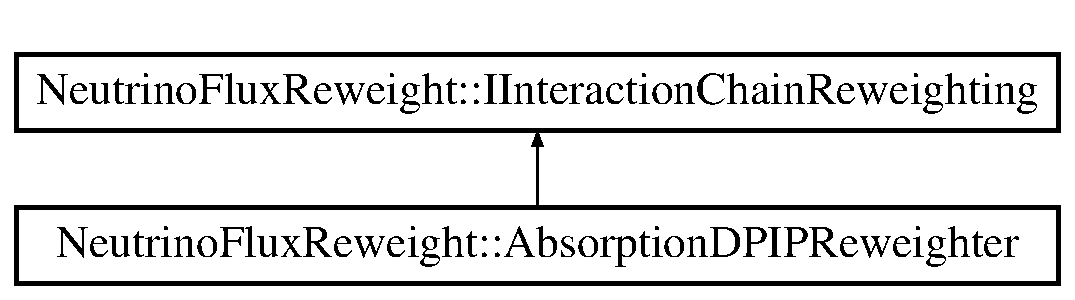
\includegraphics[height=2.000000cm]{class_neutrino_flux_reweight_1_1_absorption_d_p_i_p_reweighter}
\end{center}
\end{figure}
\subsection*{Public Member Functions}
\begin{DoxyCompactItemize}
\item 
\hyperlink{class_neutrino_flux_reweight_1_1_absorption_d_p_i_p_reweighter_a3665b9d316e77f15a25c032a091271e1}{Absorption\-D\-P\-I\-P\-Reweighter} (int iuniv, const \hyperlink{class_neutrino_flux_reweight_1_1_parameter_table}{Parameter\-Table} \&cv\-\_\-pars, const \hyperlink{class_neutrino_flux_reweight_1_1_parameter_table}{Parameter\-Table} \&univ\-\_\-pars)
\item 
virtual \hyperlink{class_neutrino_flux_reweight_1_1_absorption_d_p_i_p_reweighter_a61fd56f21c1b98f1b789afd9be0c659e}{$\sim$\-Absorption\-D\-P\-I\-P\-Reweighter} ()
\item 
virtual std\-::vector$<$ bool $>$ \hyperlink{class_neutrino_flux_reweight_1_1_absorption_d_p_i_p_reweighter_a9fc3f50ccda671f623473e43ba49989f}{can\-Reweight} (const \hyperlink{class_neutrino_flux_reweight_1_1_interaction_chain_data}{Interaction\-Chain\-Data} \&aa)
\begin{DoxyCompactList}\small\item\em Look through the \hyperlink{class_neutrino_flux_reweight_1_1_interaction_chain_data}{Interaction\-Chain\-Data} input and identify those Interactions that can be reweighted as part of a chain. We return a vector indicating which elements will be assigned a weight by calculate\-Weight. \end{DoxyCompactList}\item 
virtual double \hyperlink{class_neutrino_flux_reweight_1_1_absorption_d_p_i_p_reweighter_a8b1fcaecb31a3612ec2f5e2a0026bcb6}{calculate\-Weight} (const \hyperlink{class_neutrino_flux_reweight_1_1_interaction_chain_data}{Interaction\-Chain\-Data} \&aa)
\begin{DoxyCompactList}\small\item\em calculate a weight for this interaction chain given the central value parameters and the parameters for this universe. The weight is something like\-: f(cv)/f(M\-C) $\ast$ f(univ)/f(cv) where cv in this case corresponds to the best value of the parameter, given the data. If univ\-\_\-pars=cv\-\_\-pars then we are calculating a central value weight. Note, \hyperlink{class_neutrino_flux_reweight_1_1_absorption_d_p_i_p_reweighter_a9fc3f50ccda671f623473e43ba49989f}{can\-Reweight()} should be called to determine which elements of the chain are covered by the weight returned by \hyperlink{class_neutrino_flux_reweight_1_1_absorption_d_p_i_p_reweighter_a8b1fcaecb31a3612ec2f5e2a0026bcb6}{calculate\-Weight()} \end{DoxyCompactList}\end{DoxyCompactItemize}
\subsection*{Public Attributes}
\begin{DoxyCompactItemize}
\item 
const \hyperlink{class_neutrino_flux_reweight_1_1_parameter_table}{Parameter\-Table} \& \hyperlink{class_neutrino_flux_reweight_1_1_absorption_d_p_i_p_reweighter_ab830029670dfde65be3fc9a0bc40cd49}{cv\-Pars}
\item 
const \hyperlink{class_neutrino_flux_reweight_1_1_parameter_table}{Parameter\-Table} \& \hyperlink{class_neutrino_flux_reweight_1_1_absorption_d_p_i_p_reweighter_a47776d1d928633d93087b6fc9570f72d}{univ\-Pars}
\end{DoxyCompactItemize}
\subsection*{Private Attributes}
\begin{DoxyCompactItemize}
\item 
int \hyperlink{class_neutrino_flux_reweight_1_1_absorption_d_p_i_p_reweighter_a148d5a14a463e38ef23ed9511d26ba8f}{i\-Univ}
\item 
float \hyperlink{class_neutrino_flux_reweight_1_1_absorption_d_p_i_p_reweighter_af745299f29459ca26ac57b9bae817bdb}{inel\-\_\-pi\-Al\-\_\-xsec}
\item 
float \hyperlink{class_neutrino_flux_reweight_1_1_absorption_d_p_i_p_reweighter_a7035ed9b51c4053c042dd791bbe837d6}{inel\-\_\-kap\-Al\-\_\-xsec\-\_\-low\-P}
\item 
float \hyperlink{class_neutrino_flux_reweight_1_1_absorption_d_p_i_p_reweighter_a4c5d6fe2c15175a60e2641ae1c714408}{inel\-\_\-kap\-Al\-\_\-xsec\-\_\-high\-P}
\item 
float \hyperlink{class_neutrino_flux_reweight_1_1_absorption_d_p_i_p_reweighter_a3cef22dec7205f0331beb41c2eb35238}{inel\-\_\-kam\-Al\-\_\-xsec\-\_\-low\-P}
\item 
float \hyperlink{class_neutrino_flux_reweight_1_1_absorption_d_p_i_p_reweighter_a97ba47996c1cae70e4374d8856fdb4cd}{inel\-\_\-kam\-Al\-\_\-xsec\-\_\-high\-P}
\end{DoxyCompactItemize}


\subsection{Detailed Description}


Definition at line 17 of file Absorption\-D\-P\-I\-P\-Reweighter.\-h.



\subsection{Constructor \& Destructor Documentation}
\hypertarget{class_neutrino_flux_reweight_1_1_absorption_d_p_i_p_reweighter_a3665b9d316e77f15a25c032a091271e1}{\index{Neutrino\-Flux\-Reweight\-::\-Absorption\-D\-P\-I\-P\-Reweighter@{Neutrino\-Flux\-Reweight\-::\-Absorption\-D\-P\-I\-P\-Reweighter}!Absorption\-D\-P\-I\-P\-Reweighter@{Absorption\-D\-P\-I\-P\-Reweighter}}
\index{Absorption\-D\-P\-I\-P\-Reweighter@{Absorption\-D\-P\-I\-P\-Reweighter}!NeutrinoFluxReweight::AbsorptionDPIPReweighter@{Neutrino\-Flux\-Reweight\-::\-Absorption\-D\-P\-I\-P\-Reweighter}}
\subsubsection[{Absorption\-D\-P\-I\-P\-Reweighter}]{\setlength{\rightskip}{0pt plus 5cm}Neutrino\-Flux\-Reweight\-::\-Absorption\-D\-P\-I\-P\-Reweighter\-::\-Absorption\-D\-P\-I\-P\-Reweighter (
\begin{DoxyParamCaption}
\item[{int}]{iuniv, }
\item[{const {\bf Parameter\-Table} \&}]{cv\-\_\-pars, }
\item[{const {\bf Parameter\-Table} \&}]{univ\-\_\-pars}
\end{DoxyParamCaption}
)}}\label{class_neutrino_flux_reweight_1_1_absorption_d_p_i_p_reweighter_a3665b9d316e77f15a25c032a091271e1}
The constructor. Note, we pass central value and single universe parameters in this constructor only. There is thus a 1 to 1 correspondence between an instance of this class and a given universe. 

Definition at line 12 of file Absorption\-D\-P\-I\-P\-Reweighter.\-cpp.


\begin{DoxyCode}
12                                                                                                            
                        :\hyperlink{class_neutrino_flux_reweight_1_1_absorption_d_p_i_p_reweighter_ab830029670dfde65be3fc9a0bc40cd49}{cvPars}(cv\_pars),\hyperlink{class_neutrino_flux_reweight_1_1_absorption_d_p_i_p_reweighter_a47776d1d928633d93087b6fc9570f72d}{univPars}(univ\_pars),\hyperlink{class_neutrino_flux_reweight_1_1_absorption_d_p_i_p_reweighter_a148d5a14a463e38ef23ed9511d26ba8f}{iUniv}(iuniv)\{ 
13     
14     \textcolor{comment}{// const boost::interprocess::flat\_map<std::string, double>& dsig\_table = univPars.getMap();}
15     \hyperlink{class_neutrino_flux_reweight_1_1_absorption_d_p_i_p_reweighter_af745299f29459ca26ac57b9bae817bdb}{inel\_piAl\_xsec} = \hyperlink{class_neutrino_flux_reweight_1_1_absorption_d_p_i_p_reweighter_a47776d1d928633d93087b6fc9570f72d}{univPars}.\hyperlink{class_neutrino_flux_reweight_1_1_parameter_table_acb7dc8335b65b116f6092f2fa57ca5ed}{getParameterValue}(\textcolor{stringliteral}{"inel\_piAl\_xsec"});
16     \hyperlink{class_neutrino_flux_reweight_1_1_absorption_d_p_i_p_reweighter_a7035ed9b51c4053c042dd791bbe837d6}{inel\_kapAl\_xsec\_lowP}  = \hyperlink{class_neutrino_flux_reweight_1_1_absorption_d_p_i_p_reweighter_a47776d1d928633d93087b6fc9570f72d}{univPars}.
      \hyperlink{class_neutrino_flux_reweight_1_1_parameter_table_acb7dc8335b65b116f6092f2fa57ca5ed}{getParameterValue}(\textcolor{stringliteral}{"inel\_kapAl\_xsec\_lowP"});
17     \hyperlink{class_neutrino_flux_reweight_1_1_absorption_d_p_i_p_reweighter_a4c5d6fe2c15175a60e2641ae1c714408}{inel\_kapAl\_xsec\_highP} = \hyperlink{class_neutrino_flux_reweight_1_1_absorption_d_p_i_p_reweighter_a47776d1d928633d93087b6fc9570f72d}{univPars}.
      \hyperlink{class_neutrino_flux_reweight_1_1_parameter_table_acb7dc8335b65b116f6092f2fa57ca5ed}{getParameterValue}(\textcolor{stringliteral}{"inel\_kapAl\_xsec\_highP"});
18     \hyperlink{class_neutrino_flux_reweight_1_1_absorption_d_p_i_p_reweighter_a3cef22dec7205f0331beb41c2eb35238}{inel\_kamAl\_xsec\_lowP}  = \hyperlink{class_neutrino_flux_reweight_1_1_absorption_d_p_i_p_reweighter_a47776d1d928633d93087b6fc9570f72d}{univPars}.
      \hyperlink{class_neutrino_flux_reweight_1_1_parameter_table_acb7dc8335b65b116f6092f2fa57ca5ed}{getParameterValue}(\textcolor{stringliteral}{"inel\_kamAl\_xsec\_lowP"});
19     \hyperlink{class_neutrino_flux_reweight_1_1_absorption_d_p_i_p_reweighter_a97ba47996c1cae70e4374d8856fdb4cd}{inel\_kamAl\_xsec\_highP} = \hyperlink{class_neutrino_flux_reweight_1_1_absorption_d_p_i_p_reweighter_a47776d1d928633d93087b6fc9570f72d}{univPars}.
      \hyperlink{class_neutrino_flux_reweight_1_1_parameter_table_acb7dc8335b65b116f6092f2fa57ca5ed}{getParameterValue}(\textcolor{stringliteral}{"inel\_kamAl\_xsec\_highP"});
20     
21   \}
\end{DoxyCode}
\hypertarget{class_neutrino_flux_reweight_1_1_absorption_d_p_i_p_reweighter_a61fd56f21c1b98f1b789afd9be0c659e}{\index{Neutrino\-Flux\-Reweight\-::\-Absorption\-D\-P\-I\-P\-Reweighter@{Neutrino\-Flux\-Reweight\-::\-Absorption\-D\-P\-I\-P\-Reweighter}!$\sim$\-Absorption\-D\-P\-I\-P\-Reweighter@{$\sim$\-Absorption\-D\-P\-I\-P\-Reweighter}}
\index{$\sim$\-Absorption\-D\-P\-I\-P\-Reweighter@{$\sim$\-Absorption\-D\-P\-I\-P\-Reweighter}!NeutrinoFluxReweight::AbsorptionDPIPReweighter@{Neutrino\-Flux\-Reweight\-::\-Absorption\-D\-P\-I\-P\-Reweighter}}
\subsubsection[{$\sim$\-Absorption\-D\-P\-I\-P\-Reweighter}]{\setlength{\rightskip}{0pt plus 5cm}Neutrino\-Flux\-Reweight\-::\-Absorption\-D\-P\-I\-P\-Reweighter\-::$\sim$\-Absorption\-D\-P\-I\-P\-Reweighter (
\begin{DoxyParamCaption}
{}
\end{DoxyParamCaption}
)\hspace{0.3cm}{\ttfamily [virtual]}}}\label{class_neutrino_flux_reweight_1_1_absorption_d_p_i_p_reweighter_a61fd56f21c1b98f1b789afd9be0c659e}


Definition at line 22 of file Absorption\-D\-P\-I\-P\-Reweighter.\-cpp.


\begin{DoxyCode}
22                                                      \{
23     
24   \}
\end{DoxyCode}


\subsection{Member Function Documentation}
\hypertarget{class_neutrino_flux_reweight_1_1_absorption_d_p_i_p_reweighter_a8b1fcaecb31a3612ec2f5e2a0026bcb6}{\index{Neutrino\-Flux\-Reweight\-::\-Absorption\-D\-P\-I\-P\-Reweighter@{Neutrino\-Flux\-Reweight\-::\-Absorption\-D\-P\-I\-P\-Reweighter}!calculate\-Weight@{calculate\-Weight}}
\index{calculate\-Weight@{calculate\-Weight}!NeutrinoFluxReweight::AbsorptionDPIPReweighter@{Neutrino\-Flux\-Reweight\-::\-Absorption\-D\-P\-I\-P\-Reweighter}}
\subsubsection[{calculate\-Weight}]{\setlength{\rightskip}{0pt plus 5cm}double Neutrino\-Flux\-Reweight\-::\-Absorption\-D\-P\-I\-P\-Reweighter\-::calculate\-Weight (
\begin{DoxyParamCaption}
\item[{const {\bf Interaction\-Chain\-Data} \&}]{aa}
\end{DoxyParamCaption}
)\hspace{0.3cm}{\ttfamily [virtual]}}}\label{class_neutrino_flux_reweight_1_1_absorption_d_p_i_p_reweighter_a8b1fcaecb31a3612ec2f5e2a0026bcb6}


calculate a weight for this interaction chain given the central value parameters and the parameters for this universe. The weight is something like\-: f(cv)/f(M\-C) $\ast$ f(univ)/f(cv) where cv in this case corresponds to the best value of the parameter, given the data. If univ\-\_\-pars=cv\-\_\-pars then we are calculating a central value weight. Note, \hyperlink{class_neutrino_flux_reweight_1_1_absorption_d_p_i_p_reweighter_a9fc3f50ccda671f623473e43ba49989f}{can\-Reweight()} should be called to determine which elements of the chain are covered by the weight returned by \hyperlink{class_neutrino_flux_reweight_1_1_absorption_d_p_i_p_reweighter_a8b1fcaecb31a3612ec2f5e2a0026bcb6}{calculate\-Weight()} 



Implements \hyperlink{class_neutrino_flux_reweight_1_1_i_interaction_chain_reweighting_ae28403553637013fdc720674ee24c7c5}{Neutrino\-Flux\-Reweight\-::\-I\-Interaction\-Chain\-Reweighting}.



Definition at line 42 of file Absorption\-D\-P\-I\-P\-Reweighter.\-cpp.


\begin{DoxyCode}
42                                                                                 \{
43     
44     std::vector<ParticlesThroughVolumesData>  vec\_ptv = aa.ptv\_info;
45     std::string namepar;
46     \textcolor{keywordtype}{double} NA\_mb    = 6.02E-4; \textcolor{comment}{// how is this number computed? Does it depend on material?}
47     \textcolor{keywordtype}{double} wgt      = 1.0;
48     \textcolor{keywordtype}{double} tot\_dist = 0.0;
49     \textcolor{keywordtype}{double} low\_val  = 1.E-20;   
50     \textcolor{keywordtype}{int} index\_vol   = 1;
51     
52     \textcolor{keywordflow}{for}(\textcolor{keywordtype}{int} ii=0;ii<3;ii++)\{
53       \textcolor{keywordtype}{float} shift = 0.0;
54       tot\_dist = vec\_ptv[index\_vol].AmountMat[ii];
55       \textcolor{keywordflow}{if}(tot\_dist<low\_val)\textcolor{keywordflow}{continue};
56       \textcolor{keywordflow}{if}(abs(vec\_ptv[index\_vol].Pdgs[ii])!=321 && abs(vec\_ptv[index\_vol].Pdgs[ii])!=211)\textcolor{keywordflow}{continue};
57       
58       \textcolor{comment}{// what are the units of shift?}
59       \textcolor{keywordflow}{if}(abs(vec\_ptv[index\_vol].Pdgs[ii])== 211)shift = \hyperlink{class_neutrino_flux_reweight_1_1_absorption_d_p_i_p_reweighter_af745299f29459ca26ac57b9bae817bdb}{inel\_piAl\_xsec};
60       \textcolor{keywordflow}{else} \textcolor{keywordflow}{if}(vec\_ptv[index\_vol].Pdgs[ii]== 321 && vec\_ptv[index\_vol].Moms[ii]<2.0)shift = 
      \hyperlink{class_neutrino_flux_reweight_1_1_absorption_d_p_i_p_reweighter_a7035ed9b51c4053c042dd791bbe837d6}{inel\_kapAl\_xsec\_lowP};
61       \textcolor{keywordflow}{else} \textcolor{keywordflow}{if}(vec\_ptv[index\_vol].Pdgs[ii]== 321 && vec\_ptv[index\_vol].Moms[ii]>2.0)shift = 
      \hyperlink{class_neutrino_flux_reweight_1_1_absorption_d_p_i_p_reweighter_a4c5d6fe2c15175a60e2641ae1c714408}{inel\_kapAl\_xsec\_highP};
62       \textcolor{keywordflow}{else} \textcolor{keywordflow}{if}(vec\_ptv[index\_vol].Pdgs[ii]==-321 && vec\_ptv[index\_vol].Moms[ii]<2.0)shift = 
      \hyperlink{class_neutrino_flux_reweight_1_1_absorption_d_p_i_p_reweighter_a3cef22dec7205f0331beb41c2eb35238}{inel\_kamAl\_xsec\_lowP};
63       \textcolor{keywordflow}{else} \textcolor{keywordflow}{if}(vec\_ptv[index\_vol].Pdgs[ii]==-321 && vec\_ptv[index\_vol].Moms[ii]>2.0)shift = 
      \hyperlink{class_neutrino_flux_reweight_1_1_absorption_d_p_i_p_reweighter_a97ba47996c1cae70e4374d8856fdb4cd}{inel\_kamAl\_xsec\_highP};
64       
65       tot\_dist *= NA\_mb;
66       tot\_dist *= shift;
67       
68       wgt *= exp(-1.0*tot\_dist);   
69     \}
70     
71     \textcolor{keywordflow}{return} wgt;
72 
73   \}
\end{DoxyCode}
\hypertarget{class_neutrino_flux_reweight_1_1_absorption_d_p_i_p_reweighter_a9fc3f50ccda671f623473e43ba49989f}{\index{Neutrino\-Flux\-Reweight\-::\-Absorption\-D\-P\-I\-P\-Reweighter@{Neutrino\-Flux\-Reweight\-::\-Absorption\-D\-P\-I\-P\-Reweighter}!can\-Reweight@{can\-Reweight}}
\index{can\-Reweight@{can\-Reweight}!NeutrinoFluxReweight::AbsorptionDPIPReweighter@{Neutrino\-Flux\-Reweight\-::\-Absorption\-D\-P\-I\-P\-Reweighter}}
\subsubsection[{can\-Reweight}]{\setlength{\rightskip}{0pt plus 5cm}std\-::vector$<$ bool $>$ Neutrino\-Flux\-Reweight\-::\-Absorption\-D\-P\-I\-P\-Reweighter\-::can\-Reweight (
\begin{DoxyParamCaption}
\item[{const {\bf Interaction\-Chain\-Data} \&}]{aa}
\end{DoxyParamCaption}
)\hspace{0.3cm}{\ttfamily [virtual]}}}\label{class_neutrino_flux_reweight_1_1_absorption_d_p_i_p_reweighter_a9fc3f50ccda671f623473e43ba49989f}


Look through the \hyperlink{class_neutrino_flux_reweight_1_1_interaction_chain_data}{Interaction\-Chain\-Data} input and identify those Interactions that can be reweighted as part of a chain. We return a vector indicating which elements will be assigned a weight by calculate\-Weight. 



Implements \hyperlink{class_neutrino_flux_reweight_1_1_i_interaction_chain_reweighting_aacf17580c1d316f0ebcdfdff7418e9e3}{Neutrino\-Flux\-Reweight\-::\-I\-Interaction\-Chain\-Reweighting}.



Definition at line 25 of file Absorption\-D\-P\-I\-P\-Reweighter.\-cpp.


\begin{DoxyCode}
25                                                                                      \{
26     
27     std::vector<bool> this\_nodes;
28     \textcolor{keywordtype}{int} index\_vol = 1;
29     \textcolor{keywordtype}{double} low\_val = 1.E-20;    
30 
31     std::vector<ParticlesThroughVolumesData>  vec\_ptv = aa.ptv\_info;
32 
33     \textcolor{keywordtype}{bool} passVOL = \textcolor{keyword}{false};
34     \textcolor{comment}{//Cheking at least one ancestor with amount of materail value:}
35     \textcolor{keywordflow}{for}(\textcolor{keywordtype}{int} ii=0;ii<3;ii++)\{
36       passVOL = passVOL || (vec\_ptv[index\_vol].AmountMat[ii] >low\_val && (abs(vec\_ptv[index\_vol].Pdgs[ii])=
      =211 || abs(vec\_ptv[index\_vol].Pdgs[ii])==321));
37     \}
38     this\_nodes.push\_back(passVOL);
39     \textcolor{keywordflow}{return} this\_nodes;
40     
41   \}
\end{DoxyCode}


\subsection{Member Data Documentation}
\hypertarget{class_neutrino_flux_reweight_1_1_absorption_d_p_i_p_reweighter_ab830029670dfde65be3fc9a0bc40cd49}{\index{Neutrino\-Flux\-Reweight\-::\-Absorption\-D\-P\-I\-P\-Reweighter@{Neutrino\-Flux\-Reweight\-::\-Absorption\-D\-P\-I\-P\-Reweighter}!cv\-Pars@{cv\-Pars}}
\index{cv\-Pars@{cv\-Pars}!NeutrinoFluxReweight::AbsorptionDPIPReweighter@{Neutrino\-Flux\-Reweight\-::\-Absorption\-D\-P\-I\-P\-Reweighter}}
\subsubsection[{cv\-Pars}]{\setlength{\rightskip}{0pt plus 5cm}const {\bf Parameter\-Table}\& Neutrino\-Flux\-Reweight\-::\-Absorption\-D\-P\-I\-P\-Reweighter\-::cv\-Pars}}\label{class_neutrino_flux_reweight_1_1_absorption_d_p_i_p_reweighter_ab830029670dfde65be3fc9a0bc40cd49}


Definition at line 29 of file Absorption\-D\-P\-I\-P\-Reweighter.\-h.

\hypertarget{class_neutrino_flux_reweight_1_1_absorption_d_p_i_p_reweighter_a97ba47996c1cae70e4374d8856fdb4cd}{\index{Neutrino\-Flux\-Reweight\-::\-Absorption\-D\-P\-I\-P\-Reweighter@{Neutrino\-Flux\-Reweight\-::\-Absorption\-D\-P\-I\-P\-Reweighter}!inel\-\_\-kam\-Al\-\_\-xsec\-\_\-high\-P@{inel\-\_\-kam\-Al\-\_\-xsec\-\_\-high\-P}}
\index{inel\-\_\-kam\-Al\-\_\-xsec\-\_\-high\-P@{inel\-\_\-kam\-Al\-\_\-xsec\-\_\-high\-P}!NeutrinoFluxReweight::AbsorptionDPIPReweighter@{Neutrino\-Flux\-Reweight\-::\-Absorption\-D\-P\-I\-P\-Reweighter}}
\subsubsection[{inel\-\_\-kam\-Al\-\_\-xsec\-\_\-high\-P}]{\setlength{\rightskip}{0pt plus 5cm}float Neutrino\-Flux\-Reweight\-::\-Absorption\-D\-P\-I\-P\-Reweighter\-::inel\-\_\-kam\-Al\-\_\-xsec\-\_\-high\-P\hspace{0.3cm}{\ttfamily [private]}}}\label{class_neutrino_flux_reweight_1_1_absorption_d_p_i_p_reweighter_a97ba47996c1cae70e4374d8856fdb4cd}


Definition at line 36 of file Absorption\-D\-P\-I\-P\-Reweighter.\-h.

\hypertarget{class_neutrino_flux_reweight_1_1_absorption_d_p_i_p_reweighter_a3cef22dec7205f0331beb41c2eb35238}{\index{Neutrino\-Flux\-Reweight\-::\-Absorption\-D\-P\-I\-P\-Reweighter@{Neutrino\-Flux\-Reweight\-::\-Absorption\-D\-P\-I\-P\-Reweighter}!inel\-\_\-kam\-Al\-\_\-xsec\-\_\-low\-P@{inel\-\_\-kam\-Al\-\_\-xsec\-\_\-low\-P}}
\index{inel\-\_\-kam\-Al\-\_\-xsec\-\_\-low\-P@{inel\-\_\-kam\-Al\-\_\-xsec\-\_\-low\-P}!NeutrinoFluxReweight::AbsorptionDPIPReweighter@{Neutrino\-Flux\-Reweight\-::\-Absorption\-D\-P\-I\-P\-Reweighter}}
\subsubsection[{inel\-\_\-kam\-Al\-\_\-xsec\-\_\-low\-P}]{\setlength{\rightskip}{0pt plus 5cm}float Neutrino\-Flux\-Reweight\-::\-Absorption\-D\-P\-I\-P\-Reweighter\-::inel\-\_\-kam\-Al\-\_\-xsec\-\_\-low\-P\hspace{0.3cm}{\ttfamily [private]}}}\label{class_neutrino_flux_reweight_1_1_absorption_d_p_i_p_reweighter_a3cef22dec7205f0331beb41c2eb35238}


Definition at line 36 of file Absorption\-D\-P\-I\-P\-Reweighter.\-h.

\hypertarget{class_neutrino_flux_reweight_1_1_absorption_d_p_i_p_reweighter_a4c5d6fe2c15175a60e2641ae1c714408}{\index{Neutrino\-Flux\-Reweight\-::\-Absorption\-D\-P\-I\-P\-Reweighter@{Neutrino\-Flux\-Reweight\-::\-Absorption\-D\-P\-I\-P\-Reweighter}!inel\-\_\-kap\-Al\-\_\-xsec\-\_\-high\-P@{inel\-\_\-kap\-Al\-\_\-xsec\-\_\-high\-P}}
\index{inel\-\_\-kap\-Al\-\_\-xsec\-\_\-high\-P@{inel\-\_\-kap\-Al\-\_\-xsec\-\_\-high\-P}!NeutrinoFluxReweight::AbsorptionDPIPReweighter@{Neutrino\-Flux\-Reweight\-::\-Absorption\-D\-P\-I\-P\-Reweighter}}
\subsubsection[{inel\-\_\-kap\-Al\-\_\-xsec\-\_\-high\-P}]{\setlength{\rightskip}{0pt plus 5cm}float Neutrino\-Flux\-Reweight\-::\-Absorption\-D\-P\-I\-P\-Reweighter\-::inel\-\_\-kap\-Al\-\_\-xsec\-\_\-high\-P\hspace{0.3cm}{\ttfamily [private]}}}\label{class_neutrino_flux_reweight_1_1_absorption_d_p_i_p_reweighter_a4c5d6fe2c15175a60e2641ae1c714408}


Definition at line 35 of file Absorption\-D\-P\-I\-P\-Reweighter.\-h.

\hypertarget{class_neutrino_flux_reweight_1_1_absorption_d_p_i_p_reweighter_a7035ed9b51c4053c042dd791bbe837d6}{\index{Neutrino\-Flux\-Reweight\-::\-Absorption\-D\-P\-I\-P\-Reweighter@{Neutrino\-Flux\-Reweight\-::\-Absorption\-D\-P\-I\-P\-Reweighter}!inel\-\_\-kap\-Al\-\_\-xsec\-\_\-low\-P@{inel\-\_\-kap\-Al\-\_\-xsec\-\_\-low\-P}}
\index{inel\-\_\-kap\-Al\-\_\-xsec\-\_\-low\-P@{inel\-\_\-kap\-Al\-\_\-xsec\-\_\-low\-P}!NeutrinoFluxReweight::AbsorptionDPIPReweighter@{Neutrino\-Flux\-Reweight\-::\-Absorption\-D\-P\-I\-P\-Reweighter}}
\subsubsection[{inel\-\_\-kap\-Al\-\_\-xsec\-\_\-low\-P}]{\setlength{\rightskip}{0pt plus 5cm}float Neutrino\-Flux\-Reweight\-::\-Absorption\-D\-P\-I\-P\-Reweighter\-::inel\-\_\-kap\-Al\-\_\-xsec\-\_\-low\-P\hspace{0.3cm}{\ttfamily [private]}}}\label{class_neutrino_flux_reweight_1_1_absorption_d_p_i_p_reweighter_a7035ed9b51c4053c042dd791bbe837d6}


Definition at line 35 of file Absorption\-D\-P\-I\-P\-Reweighter.\-h.

\hypertarget{class_neutrino_flux_reweight_1_1_absorption_d_p_i_p_reweighter_af745299f29459ca26ac57b9bae817bdb}{\index{Neutrino\-Flux\-Reweight\-::\-Absorption\-D\-P\-I\-P\-Reweighter@{Neutrino\-Flux\-Reweight\-::\-Absorption\-D\-P\-I\-P\-Reweighter}!inel\-\_\-pi\-Al\-\_\-xsec@{inel\-\_\-pi\-Al\-\_\-xsec}}
\index{inel\-\_\-pi\-Al\-\_\-xsec@{inel\-\_\-pi\-Al\-\_\-xsec}!NeutrinoFluxReweight::AbsorptionDPIPReweighter@{Neutrino\-Flux\-Reweight\-::\-Absorption\-D\-P\-I\-P\-Reweighter}}
\subsubsection[{inel\-\_\-pi\-Al\-\_\-xsec}]{\setlength{\rightskip}{0pt plus 5cm}float Neutrino\-Flux\-Reweight\-::\-Absorption\-D\-P\-I\-P\-Reweighter\-::inel\-\_\-pi\-Al\-\_\-xsec\hspace{0.3cm}{\ttfamily [private]}}}\label{class_neutrino_flux_reweight_1_1_absorption_d_p_i_p_reweighter_af745299f29459ca26ac57b9bae817bdb}


Definition at line 34 of file Absorption\-D\-P\-I\-P\-Reweighter.\-h.

\hypertarget{class_neutrino_flux_reweight_1_1_absorption_d_p_i_p_reweighter_a148d5a14a463e38ef23ed9511d26ba8f}{\index{Neutrino\-Flux\-Reweight\-::\-Absorption\-D\-P\-I\-P\-Reweighter@{Neutrino\-Flux\-Reweight\-::\-Absorption\-D\-P\-I\-P\-Reweighter}!i\-Univ@{i\-Univ}}
\index{i\-Univ@{i\-Univ}!NeutrinoFluxReweight::AbsorptionDPIPReweighter@{Neutrino\-Flux\-Reweight\-::\-Absorption\-D\-P\-I\-P\-Reweighter}}
\subsubsection[{i\-Univ}]{\setlength{\rightskip}{0pt plus 5cm}int Neutrino\-Flux\-Reweight\-::\-Absorption\-D\-P\-I\-P\-Reweighter\-::i\-Univ\hspace{0.3cm}{\ttfamily [private]}}}\label{class_neutrino_flux_reweight_1_1_absorption_d_p_i_p_reweighter_a148d5a14a463e38ef23ed9511d26ba8f}


Definition at line 33 of file Absorption\-D\-P\-I\-P\-Reweighter.\-h.

\hypertarget{class_neutrino_flux_reweight_1_1_absorption_d_p_i_p_reweighter_a47776d1d928633d93087b6fc9570f72d}{\index{Neutrino\-Flux\-Reweight\-::\-Absorption\-D\-P\-I\-P\-Reweighter@{Neutrino\-Flux\-Reweight\-::\-Absorption\-D\-P\-I\-P\-Reweighter}!univ\-Pars@{univ\-Pars}}
\index{univ\-Pars@{univ\-Pars}!NeutrinoFluxReweight::AbsorptionDPIPReweighter@{Neutrino\-Flux\-Reweight\-::\-Absorption\-D\-P\-I\-P\-Reweighter}}
\subsubsection[{univ\-Pars}]{\setlength{\rightskip}{0pt plus 5cm}const {\bf Parameter\-Table}\& Neutrino\-Flux\-Reweight\-::\-Absorption\-D\-P\-I\-P\-Reweighter\-::univ\-Pars}}\label{class_neutrino_flux_reweight_1_1_absorption_d_p_i_p_reweighter_a47776d1d928633d93087b6fc9570f72d}


Definition at line 30 of file Absorption\-D\-P\-I\-P\-Reweighter.\-h.



The documentation for this class was generated from the following files\-:\begin{DoxyCompactItemize}
\item 
include/\hyperlink{_absorption_d_p_i_p_reweighter_8h}{Absorption\-D\-P\-I\-P\-Reweighter.\-h}\item 
src/\hyperlink{_absorption_d_p_i_p_reweighter_8cpp}{Absorption\-D\-P\-I\-P\-Reweighter.\-cpp}\end{DoxyCompactItemize}

\hypertarget{class_neutrino_flux_reweight_1_1_absorption_d_v_o_l_reweighter}{\section{Neutrino\-Flux\-Reweight\-:\-:Absorption\-D\-V\-O\-L\-Reweighter Class Reference}
\label{class_neutrino_flux_reweight_1_1_absorption_d_v_o_l_reweighter}\index{Neutrino\-Flux\-Reweight\-::\-Absorption\-D\-V\-O\-L\-Reweighter@{Neutrino\-Flux\-Reweight\-::\-Absorption\-D\-V\-O\-L\-Reweighter}}
}


{\ttfamily \#include $<$Absorption\-D\-V\-O\-L\-Reweighter.\-h$>$}

Inheritance diagram for Neutrino\-Flux\-Reweight\-:\-:Absorption\-D\-V\-O\-L\-Reweighter\-:\begin{figure}[H]
\begin{center}
\leavevmode
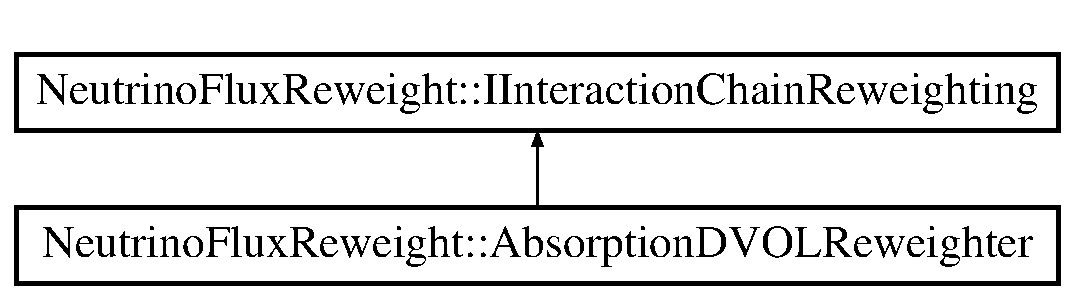
\includegraphics[height=2.000000cm]{class_neutrino_flux_reweight_1_1_absorption_d_v_o_l_reweighter}
\end{center}
\end{figure}
\subsection*{Public Member Functions}
\begin{DoxyCompactItemize}
\item 
\hyperlink{class_neutrino_flux_reweight_1_1_absorption_d_v_o_l_reweighter_a3f1c98354cf75e8cc3cea7c448a45989}{Absorption\-D\-V\-O\-L\-Reweighter} (int iuniv, const \hyperlink{class_neutrino_flux_reweight_1_1_parameter_table}{Parameter\-Table} \&cv\-\_\-pars, const \hyperlink{class_neutrino_flux_reweight_1_1_parameter_table}{Parameter\-Table} \&univ\-\_\-pars)
\item 
virtual \hyperlink{class_neutrino_flux_reweight_1_1_absorption_d_v_o_l_reweighter_a93d545e92ac458cb407ce7e219b942c2}{$\sim$\-Absorption\-D\-V\-O\-L\-Reweighter} ()
\item 
virtual std\-::vector$<$ bool $>$ \hyperlink{class_neutrino_flux_reweight_1_1_absorption_d_v_o_l_reweighter_a4431fee76a4b04a42dac9f6be83f6346}{can\-Reweight} (const \hyperlink{class_neutrino_flux_reweight_1_1_interaction_chain_data}{Interaction\-Chain\-Data} \&aa)
\begin{DoxyCompactList}\small\item\em Look through the \hyperlink{class_neutrino_flux_reweight_1_1_interaction_chain_data}{Interaction\-Chain\-Data} input and identify those Interactions that can be reweighted as part of a chain. We return a vector indicating which elements will be assigned a weight by calculate\-Weight. \end{DoxyCompactList}\item 
virtual double \hyperlink{class_neutrino_flux_reweight_1_1_absorption_d_v_o_l_reweighter_abe4d5b881334283ded041e46d2613608}{calculate\-Weight} (const \hyperlink{class_neutrino_flux_reweight_1_1_interaction_chain_data}{Interaction\-Chain\-Data} \&aa)
\begin{DoxyCompactList}\small\item\em calculate a weight for this interaction chain given the central value parameters and the parameters for this universe. The weight is something like\-: f(cv)/f(M\-C) $\ast$ f(univ)/f(cv) where cv in this case corresponds to the best value of the parameter, given the data. If univ\-\_\-pars=cv\-\_\-pars then we are calculating a central value weight. Note, \hyperlink{class_neutrino_flux_reweight_1_1_absorption_d_v_o_l_reweighter_a4431fee76a4b04a42dac9f6be83f6346}{can\-Reweight()} should be called to determine which elements of the chain are covered by the weight returned by \hyperlink{class_neutrino_flux_reweight_1_1_absorption_d_v_o_l_reweighter_abe4d5b881334283ded041e46d2613608}{calculate\-Weight()} \end{DoxyCompactList}\end{DoxyCompactItemize}
\subsection*{Public Attributes}
\begin{DoxyCompactItemize}
\item 
const \hyperlink{class_neutrino_flux_reweight_1_1_parameter_table}{Parameter\-Table} \& \hyperlink{class_neutrino_flux_reweight_1_1_absorption_d_v_o_l_reweighter_a9eab93b31a22145ef9fa33a877dbf02e}{cv\-Pars}
\item 
const \hyperlink{class_neutrino_flux_reweight_1_1_parameter_table}{Parameter\-Table} \& \hyperlink{class_neutrino_flux_reweight_1_1_absorption_d_v_o_l_reweighter_a2bb54a2f64d4cc407e3afa5bf8c298e4}{univ\-Pars}
\end{DoxyCompactItemize}
\subsection*{Private Attributes}
\begin{DoxyCompactItemize}
\item 
int \hyperlink{class_neutrino_flux_reweight_1_1_absorption_d_v_o_l_reweighter_a9a086a16ffdb3431f69c980c4f80d0b4}{i\-Univ}
\item 
float \hyperlink{class_neutrino_flux_reweight_1_1_absorption_d_v_o_l_reweighter_ab70c49c8fc53548eed60cca86589ae98}{inel\-\_\-pi\-Al\-\_\-xsec}
\item 
float \hyperlink{class_neutrino_flux_reweight_1_1_absorption_d_v_o_l_reweighter_a2d57ad8d135f3874fe5636f9a30ceea1}{inel\-\_\-kap\-Al\-\_\-xsec\-\_\-low\-P}
\item 
float \hyperlink{class_neutrino_flux_reweight_1_1_absorption_d_v_o_l_reweighter_a980a548cffd4ca6fb3df8e146f11a30d}{inel\-\_\-kap\-Al\-\_\-xsec\-\_\-high\-P}
\item 
float \hyperlink{class_neutrino_flux_reweight_1_1_absorption_d_v_o_l_reweighter_aaed12a6a79b561923f5f426de474f006}{inel\-\_\-kam\-Al\-\_\-xsec\-\_\-low\-P}
\item 
float \hyperlink{class_neutrino_flux_reweight_1_1_absorption_d_v_o_l_reweighter_a75a48086a64722329b58cd1e099933c4}{inel\-\_\-kam\-Al\-\_\-xsec\-\_\-high\-P}
\end{DoxyCompactItemize}


\subsection{Detailed Description}


Definition at line 16 of file Absorption\-D\-V\-O\-L\-Reweighter.\-h.



\subsection{Constructor \& Destructor Documentation}
\hypertarget{class_neutrino_flux_reweight_1_1_absorption_d_v_o_l_reweighter_a3f1c98354cf75e8cc3cea7c448a45989}{\index{Neutrino\-Flux\-Reweight\-::\-Absorption\-D\-V\-O\-L\-Reweighter@{Neutrino\-Flux\-Reweight\-::\-Absorption\-D\-V\-O\-L\-Reweighter}!Absorption\-D\-V\-O\-L\-Reweighter@{Absorption\-D\-V\-O\-L\-Reweighter}}
\index{Absorption\-D\-V\-O\-L\-Reweighter@{Absorption\-D\-V\-O\-L\-Reweighter}!NeutrinoFluxReweight::AbsorptionDVOLReweighter@{Neutrino\-Flux\-Reweight\-::\-Absorption\-D\-V\-O\-L\-Reweighter}}
\subsubsection[{Absorption\-D\-V\-O\-L\-Reweighter}]{\setlength{\rightskip}{0pt plus 5cm}Neutrino\-Flux\-Reweight\-::\-Absorption\-D\-V\-O\-L\-Reweighter\-::\-Absorption\-D\-V\-O\-L\-Reweighter (
\begin{DoxyParamCaption}
\item[{int}]{iuniv, }
\item[{const {\bf Parameter\-Table} \&}]{cv\-\_\-pars, }
\item[{const {\bf Parameter\-Table} \&}]{univ\-\_\-pars}
\end{DoxyParamCaption}
)}}\label{class_neutrino_flux_reweight_1_1_absorption_d_v_o_l_reweighter_a3f1c98354cf75e8cc3cea7c448a45989}
The constructor. Note, we pass central value and single universe parameters in this constructor only. There is thus a 1 to 1 correspondence between an instance of this class and a given universe. 

Definition at line 12 of file Absorption\-D\-V\-O\-L\-Reweighter.\-cpp.


\begin{DoxyCode}
12                                                                                                            
                        :\hyperlink{class_neutrino_flux_reweight_1_1_absorption_d_v_o_l_reweighter_a9eab93b31a22145ef9fa33a877dbf02e}{cvPars}(cv\_pars),\hyperlink{class_neutrino_flux_reweight_1_1_absorption_d_v_o_l_reweighter_a2bb54a2f64d4cc407e3afa5bf8c298e4}{univPars}(univ\_pars),\hyperlink{class_neutrino_flux_reweight_1_1_absorption_d_v_o_l_reweighter_a9a086a16ffdb3431f69c980c4f80d0b4}{iUniv}(iuniv)\{ 
13     
14     \textcolor{comment}{// const boost::interprocess::flat\_map<std::string, double>& dsig\_table = univPars.getMap();}
15     \hyperlink{class_neutrino_flux_reweight_1_1_absorption_d_v_o_l_reweighter_ab70c49c8fc53548eed60cca86589ae98}{inel\_piAl\_xsec} = \hyperlink{class_neutrino_flux_reweight_1_1_absorption_d_v_o_l_reweighter_a2bb54a2f64d4cc407e3afa5bf8c298e4}{univPars}.\hyperlink{class_neutrino_flux_reweight_1_1_parameter_table_acb7dc8335b65b116f6092f2fa57ca5ed}{getParameterValue}(\textcolor{stringliteral}{"inel\_piAl\_xsec"});
16     \hyperlink{class_neutrino_flux_reweight_1_1_absorption_d_v_o_l_reweighter_a2d57ad8d135f3874fe5636f9a30ceea1}{inel\_kapAl\_xsec\_lowP}  = \hyperlink{class_neutrino_flux_reweight_1_1_absorption_d_v_o_l_reweighter_a2bb54a2f64d4cc407e3afa5bf8c298e4}{univPars}.
      \hyperlink{class_neutrino_flux_reweight_1_1_parameter_table_acb7dc8335b65b116f6092f2fa57ca5ed}{getParameterValue}(\textcolor{stringliteral}{"inel\_kapAl\_xsec\_lowP"});
17     \hyperlink{class_neutrino_flux_reweight_1_1_absorption_d_v_o_l_reweighter_a980a548cffd4ca6fb3df8e146f11a30d}{inel\_kapAl\_xsec\_highP} = \hyperlink{class_neutrino_flux_reweight_1_1_absorption_d_v_o_l_reweighter_a2bb54a2f64d4cc407e3afa5bf8c298e4}{univPars}.
      \hyperlink{class_neutrino_flux_reweight_1_1_parameter_table_acb7dc8335b65b116f6092f2fa57ca5ed}{getParameterValue}(\textcolor{stringliteral}{"inel\_kapAl\_xsec\_highP"});
18     \hyperlink{class_neutrino_flux_reweight_1_1_absorption_d_v_o_l_reweighter_aaed12a6a79b561923f5f426de474f006}{inel\_kamAl\_xsec\_lowP}  = \hyperlink{class_neutrino_flux_reweight_1_1_absorption_d_v_o_l_reweighter_a2bb54a2f64d4cc407e3afa5bf8c298e4}{univPars}.
      \hyperlink{class_neutrino_flux_reweight_1_1_parameter_table_acb7dc8335b65b116f6092f2fa57ca5ed}{getParameterValue}(\textcolor{stringliteral}{"inel\_kamAl\_xsec\_lowP"});
19     \hyperlink{class_neutrino_flux_reweight_1_1_absorption_d_v_o_l_reweighter_a75a48086a64722329b58cd1e099933c4}{inel\_kamAl\_xsec\_highP} = \hyperlink{class_neutrino_flux_reweight_1_1_absorption_d_v_o_l_reweighter_a2bb54a2f64d4cc407e3afa5bf8c298e4}{univPars}.
      \hyperlink{class_neutrino_flux_reweight_1_1_parameter_table_acb7dc8335b65b116f6092f2fa57ca5ed}{getParameterValue}(\textcolor{stringliteral}{"inel\_kamAl\_xsec\_highP"});
20     
21   \}
\end{DoxyCode}
\hypertarget{class_neutrino_flux_reweight_1_1_absorption_d_v_o_l_reweighter_a93d545e92ac458cb407ce7e219b942c2}{\index{Neutrino\-Flux\-Reweight\-::\-Absorption\-D\-V\-O\-L\-Reweighter@{Neutrino\-Flux\-Reweight\-::\-Absorption\-D\-V\-O\-L\-Reweighter}!$\sim$\-Absorption\-D\-V\-O\-L\-Reweighter@{$\sim$\-Absorption\-D\-V\-O\-L\-Reweighter}}
\index{$\sim$\-Absorption\-D\-V\-O\-L\-Reweighter@{$\sim$\-Absorption\-D\-V\-O\-L\-Reweighter}!NeutrinoFluxReweight::AbsorptionDVOLReweighter@{Neutrino\-Flux\-Reweight\-::\-Absorption\-D\-V\-O\-L\-Reweighter}}
\subsubsection[{$\sim$\-Absorption\-D\-V\-O\-L\-Reweighter}]{\setlength{\rightskip}{0pt plus 5cm}Neutrino\-Flux\-Reweight\-::\-Absorption\-D\-V\-O\-L\-Reweighter\-::$\sim$\-Absorption\-D\-V\-O\-L\-Reweighter (
\begin{DoxyParamCaption}
{}
\end{DoxyParamCaption}
)\hspace{0.3cm}{\ttfamily [virtual]}}}\label{class_neutrino_flux_reweight_1_1_absorption_d_v_o_l_reweighter_a93d545e92ac458cb407ce7e219b942c2}


Definition at line 22 of file Absorption\-D\-V\-O\-L\-Reweighter.\-cpp.


\begin{DoxyCode}
22                                                      \{
23     
24   \}
\end{DoxyCode}


\subsection{Member Function Documentation}
\hypertarget{class_neutrino_flux_reweight_1_1_absorption_d_v_o_l_reweighter_abe4d5b881334283ded041e46d2613608}{\index{Neutrino\-Flux\-Reweight\-::\-Absorption\-D\-V\-O\-L\-Reweighter@{Neutrino\-Flux\-Reweight\-::\-Absorption\-D\-V\-O\-L\-Reweighter}!calculate\-Weight@{calculate\-Weight}}
\index{calculate\-Weight@{calculate\-Weight}!NeutrinoFluxReweight::AbsorptionDVOLReweighter@{Neutrino\-Flux\-Reweight\-::\-Absorption\-D\-V\-O\-L\-Reweighter}}
\subsubsection[{calculate\-Weight}]{\setlength{\rightskip}{0pt plus 5cm}double Neutrino\-Flux\-Reweight\-::\-Absorption\-D\-V\-O\-L\-Reweighter\-::calculate\-Weight (
\begin{DoxyParamCaption}
\item[{const {\bf Interaction\-Chain\-Data} \&}]{aa}
\end{DoxyParamCaption}
)\hspace{0.3cm}{\ttfamily [virtual]}}}\label{class_neutrino_flux_reweight_1_1_absorption_d_v_o_l_reweighter_abe4d5b881334283ded041e46d2613608}


calculate a weight for this interaction chain given the central value parameters and the parameters for this universe. The weight is something like\-: f(cv)/f(M\-C) $\ast$ f(univ)/f(cv) where cv in this case corresponds to the best value of the parameter, given the data. If univ\-\_\-pars=cv\-\_\-pars then we are calculating a central value weight. Note, \hyperlink{class_neutrino_flux_reweight_1_1_absorption_d_v_o_l_reweighter_a4431fee76a4b04a42dac9f6be83f6346}{can\-Reweight()} should be called to determine which elements of the chain are covered by the weight returned by \hyperlink{class_neutrino_flux_reweight_1_1_absorption_d_v_o_l_reweighter_abe4d5b881334283ded041e46d2613608}{calculate\-Weight()} 



Implements \hyperlink{class_neutrino_flux_reweight_1_1_i_interaction_chain_reweighting_ae28403553637013fdc720674ee24c7c5}{Neutrino\-Flux\-Reweight\-::\-I\-Interaction\-Chain\-Reweighting}.



Definition at line 42 of file Absorption\-D\-V\-O\-L\-Reweighter.\-cpp.


\begin{DoxyCode}
42                                                                                 \{
43     
44     std::vector<ParticlesThroughVolumesData>  vec\_ptv = aa.ptv\_info;
45     std::string namepar;
46     \textcolor{keywordtype}{double} NA\_mb    = 6.02E-4;
47     \textcolor{keywordtype}{double} wgt      = 1.0;
48     \textcolor{keywordtype}{double} tot\_dist = 0.0;
49     \textcolor{keywordtype}{double} low\_val  = 1.E-20;   
50     \textcolor{keywordtype}{int} index\_vol   = 2;
51     
52     \textcolor{keywordflow}{for}(\textcolor{keywordtype}{int} ii=0;ii<3;ii++)\{
53       \textcolor{keywordtype}{float} shift = 0.0;
54       tot\_dist = vec\_ptv[index\_vol].AmountMat[ii];
55       \textcolor{keywordflow}{if}(tot\_dist<low\_val)\textcolor{keywordflow}{continue};
56       \textcolor{keywordflow}{if}(abs(vec\_ptv[index\_vol].Pdgs[ii])!=321 && abs(vec\_ptv[index\_vol].Pdgs[ii])!=211)\textcolor{keywordflow}{continue};
57       
58       \textcolor{keywordflow}{if}(abs(vec\_ptv[index\_vol].Pdgs[ii])== 211)shift = \hyperlink{class_neutrino_flux_reweight_1_1_absorption_d_v_o_l_reweighter_ab70c49c8fc53548eed60cca86589ae98}{inel\_piAl\_xsec};
59       \textcolor{keywordflow}{else} \textcolor{keywordflow}{if}(vec\_ptv[index\_vol].Pdgs[ii]== 321 && vec\_ptv[index\_vol].Moms[ii]<2.0)shift = 
      \hyperlink{class_neutrino_flux_reweight_1_1_absorption_d_v_o_l_reweighter_a2d57ad8d135f3874fe5636f9a30ceea1}{inel\_kapAl\_xsec\_lowP};
60       \textcolor{keywordflow}{else} \textcolor{keywordflow}{if}(vec\_ptv[index\_vol].Pdgs[ii]== 321 && vec\_ptv[index\_vol].Moms[ii]>2.0)shift = 
      \hyperlink{class_neutrino_flux_reweight_1_1_absorption_d_v_o_l_reweighter_a980a548cffd4ca6fb3df8e146f11a30d}{inel\_kapAl\_xsec\_highP};
61       \textcolor{keywordflow}{else} \textcolor{keywordflow}{if}(vec\_ptv[index\_vol].Pdgs[ii]==-321 && vec\_ptv[index\_vol].Moms[ii]<2.0)shift = 
      \hyperlink{class_neutrino_flux_reweight_1_1_absorption_d_v_o_l_reweighter_aaed12a6a79b561923f5f426de474f006}{inel\_kamAl\_xsec\_lowP};
62       \textcolor{keywordflow}{else} \textcolor{keywordflow}{if}(vec\_ptv[index\_vol].Pdgs[ii]==-321 && vec\_ptv[index\_vol].Moms[ii]>2.0)shift = 
      \hyperlink{class_neutrino_flux_reweight_1_1_absorption_d_v_o_l_reweighter_a75a48086a64722329b58cd1e099933c4}{inel\_kamAl\_xsec\_highP};
63     
64       tot\_dist *= NA\_mb;
65       tot\_dist *= shift;
66       
67       wgt *= exp(-1.0*tot\_dist);   
68     \}
69     
70     \textcolor{keywordflow}{return} wgt;
71     
72   \}
\end{DoxyCode}
\hypertarget{class_neutrino_flux_reweight_1_1_absorption_d_v_o_l_reweighter_a4431fee76a4b04a42dac9f6be83f6346}{\index{Neutrino\-Flux\-Reweight\-::\-Absorption\-D\-V\-O\-L\-Reweighter@{Neutrino\-Flux\-Reweight\-::\-Absorption\-D\-V\-O\-L\-Reweighter}!can\-Reweight@{can\-Reweight}}
\index{can\-Reweight@{can\-Reweight}!NeutrinoFluxReweight::AbsorptionDVOLReweighter@{Neutrino\-Flux\-Reweight\-::\-Absorption\-D\-V\-O\-L\-Reweighter}}
\subsubsection[{can\-Reweight}]{\setlength{\rightskip}{0pt plus 5cm}std\-::vector$<$ bool $>$ Neutrino\-Flux\-Reweight\-::\-Absorption\-D\-V\-O\-L\-Reweighter\-::can\-Reweight (
\begin{DoxyParamCaption}
\item[{const {\bf Interaction\-Chain\-Data} \&}]{aa}
\end{DoxyParamCaption}
)\hspace{0.3cm}{\ttfamily [virtual]}}}\label{class_neutrino_flux_reweight_1_1_absorption_d_v_o_l_reweighter_a4431fee76a4b04a42dac9f6be83f6346}


Look through the \hyperlink{class_neutrino_flux_reweight_1_1_interaction_chain_data}{Interaction\-Chain\-Data} input and identify those Interactions that can be reweighted as part of a chain. We return a vector indicating which elements will be assigned a weight by calculate\-Weight. 



Implements \hyperlink{class_neutrino_flux_reweight_1_1_i_interaction_chain_reweighting_aacf17580c1d316f0ebcdfdff7418e9e3}{Neutrino\-Flux\-Reweight\-::\-I\-Interaction\-Chain\-Reweighting}.



Definition at line 25 of file Absorption\-D\-V\-O\-L\-Reweighter.\-cpp.


\begin{DoxyCode}
25                                                                                      \{
26  
27     std::vector<bool> this\_nodes;
28     \textcolor{keywordtype}{int} index\_vol = 2;
29     \textcolor{keywordtype}{double} low\_val = 1.E-20;    
30   
31     std::vector<ParticlesThroughVolumesData>  vec\_ptv = aa.ptv\_info;
32 
33     \textcolor{keywordtype}{bool} passVOL = \textcolor{keyword}{false};
34     \textcolor{comment}{//Cheking at least one ancestor with amount of materail value:}
35     \textcolor{keywordflow}{for}(\textcolor{keywordtype}{int} ii=0;ii<3;ii++)\{
36       passVOL = passVOL || (vec\_ptv[index\_vol].AmountMat[ii] >low\_val && (abs(vec\_ptv[index\_vol].Pdgs[ii])=
      =211 || abs(vec\_ptv[index\_vol].Pdgs[ii])==321));
37     \}
38     this\_nodes.push\_back(passVOL);
39     \textcolor{keywordflow}{return} this\_nodes;
40 
41   \}
\end{DoxyCode}


\subsection{Member Data Documentation}
\hypertarget{class_neutrino_flux_reweight_1_1_absorption_d_v_o_l_reweighter_a9eab93b31a22145ef9fa33a877dbf02e}{\index{Neutrino\-Flux\-Reweight\-::\-Absorption\-D\-V\-O\-L\-Reweighter@{Neutrino\-Flux\-Reweight\-::\-Absorption\-D\-V\-O\-L\-Reweighter}!cv\-Pars@{cv\-Pars}}
\index{cv\-Pars@{cv\-Pars}!NeutrinoFluxReweight::AbsorptionDVOLReweighter@{Neutrino\-Flux\-Reweight\-::\-Absorption\-D\-V\-O\-L\-Reweighter}}
\subsubsection[{cv\-Pars}]{\setlength{\rightskip}{0pt plus 5cm}const {\bf Parameter\-Table}\& Neutrino\-Flux\-Reweight\-::\-Absorption\-D\-V\-O\-L\-Reweighter\-::cv\-Pars}}\label{class_neutrino_flux_reweight_1_1_absorption_d_v_o_l_reweighter_a9eab93b31a22145ef9fa33a877dbf02e}


Definition at line 27 of file Absorption\-D\-V\-O\-L\-Reweighter.\-h.

\hypertarget{class_neutrino_flux_reweight_1_1_absorption_d_v_o_l_reweighter_a75a48086a64722329b58cd1e099933c4}{\index{Neutrino\-Flux\-Reweight\-::\-Absorption\-D\-V\-O\-L\-Reweighter@{Neutrino\-Flux\-Reweight\-::\-Absorption\-D\-V\-O\-L\-Reweighter}!inel\-\_\-kam\-Al\-\_\-xsec\-\_\-high\-P@{inel\-\_\-kam\-Al\-\_\-xsec\-\_\-high\-P}}
\index{inel\-\_\-kam\-Al\-\_\-xsec\-\_\-high\-P@{inel\-\_\-kam\-Al\-\_\-xsec\-\_\-high\-P}!NeutrinoFluxReweight::AbsorptionDVOLReweighter@{Neutrino\-Flux\-Reweight\-::\-Absorption\-D\-V\-O\-L\-Reweighter}}
\subsubsection[{inel\-\_\-kam\-Al\-\_\-xsec\-\_\-high\-P}]{\setlength{\rightskip}{0pt plus 5cm}float Neutrino\-Flux\-Reweight\-::\-Absorption\-D\-V\-O\-L\-Reweighter\-::inel\-\_\-kam\-Al\-\_\-xsec\-\_\-high\-P\hspace{0.3cm}{\ttfamily [private]}}}\label{class_neutrino_flux_reweight_1_1_absorption_d_v_o_l_reweighter_a75a48086a64722329b58cd1e099933c4}


Definition at line 33 of file Absorption\-D\-V\-O\-L\-Reweighter.\-h.

\hypertarget{class_neutrino_flux_reweight_1_1_absorption_d_v_o_l_reweighter_aaed12a6a79b561923f5f426de474f006}{\index{Neutrino\-Flux\-Reweight\-::\-Absorption\-D\-V\-O\-L\-Reweighter@{Neutrino\-Flux\-Reweight\-::\-Absorption\-D\-V\-O\-L\-Reweighter}!inel\-\_\-kam\-Al\-\_\-xsec\-\_\-low\-P@{inel\-\_\-kam\-Al\-\_\-xsec\-\_\-low\-P}}
\index{inel\-\_\-kam\-Al\-\_\-xsec\-\_\-low\-P@{inel\-\_\-kam\-Al\-\_\-xsec\-\_\-low\-P}!NeutrinoFluxReweight::AbsorptionDVOLReweighter@{Neutrino\-Flux\-Reweight\-::\-Absorption\-D\-V\-O\-L\-Reweighter}}
\subsubsection[{inel\-\_\-kam\-Al\-\_\-xsec\-\_\-low\-P}]{\setlength{\rightskip}{0pt plus 5cm}float Neutrino\-Flux\-Reweight\-::\-Absorption\-D\-V\-O\-L\-Reweighter\-::inel\-\_\-kam\-Al\-\_\-xsec\-\_\-low\-P\hspace{0.3cm}{\ttfamily [private]}}}\label{class_neutrino_flux_reweight_1_1_absorption_d_v_o_l_reweighter_aaed12a6a79b561923f5f426de474f006}


Definition at line 33 of file Absorption\-D\-V\-O\-L\-Reweighter.\-h.

\hypertarget{class_neutrino_flux_reweight_1_1_absorption_d_v_o_l_reweighter_a980a548cffd4ca6fb3df8e146f11a30d}{\index{Neutrino\-Flux\-Reweight\-::\-Absorption\-D\-V\-O\-L\-Reweighter@{Neutrino\-Flux\-Reweight\-::\-Absorption\-D\-V\-O\-L\-Reweighter}!inel\-\_\-kap\-Al\-\_\-xsec\-\_\-high\-P@{inel\-\_\-kap\-Al\-\_\-xsec\-\_\-high\-P}}
\index{inel\-\_\-kap\-Al\-\_\-xsec\-\_\-high\-P@{inel\-\_\-kap\-Al\-\_\-xsec\-\_\-high\-P}!NeutrinoFluxReweight::AbsorptionDVOLReweighter@{Neutrino\-Flux\-Reweight\-::\-Absorption\-D\-V\-O\-L\-Reweighter}}
\subsubsection[{inel\-\_\-kap\-Al\-\_\-xsec\-\_\-high\-P}]{\setlength{\rightskip}{0pt plus 5cm}float Neutrino\-Flux\-Reweight\-::\-Absorption\-D\-V\-O\-L\-Reweighter\-::inel\-\_\-kap\-Al\-\_\-xsec\-\_\-high\-P\hspace{0.3cm}{\ttfamily [private]}}}\label{class_neutrino_flux_reweight_1_1_absorption_d_v_o_l_reweighter_a980a548cffd4ca6fb3df8e146f11a30d}


Definition at line 32 of file Absorption\-D\-V\-O\-L\-Reweighter.\-h.

\hypertarget{class_neutrino_flux_reweight_1_1_absorption_d_v_o_l_reweighter_a2d57ad8d135f3874fe5636f9a30ceea1}{\index{Neutrino\-Flux\-Reweight\-::\-Absorption\-D\-V\-O\-L\-Reweighter@{Neutrino\-Flux\-Reweight\-::\-Absorption\-D\-V\-O\-L\-Reweighter}!inel\-\_\-kap\-Al\-\_\-xsec\-\_\-low\-P@{inel\-\_\-kap\-Al\-\_\-xsec\-\_\-low\-P}}
\index{inel\-\_\-kap\-Al\-\_\-xsec\-\_\-low\-P@{inel\-\_\-kap\-Al\-\_\-xsec\-\_\-low\-P}!NeutrinoFluxReweight::AbsorptionDVOLReweighter@{Neutrino\-Flux\-Reweight\-::\-Absorption\-D\-V\-O\-L\-Reweighter}}
\subsubsection[{inel\-\_\-kap\-Al\-\_\-xsec\-\_\-low\-P}]{\setlength{\rightskip}{0pt plus 5cm}float Neutrino\-Flux\-Reweight\-::\-Absorption\-D\-V\-O\-L\-Reweighter\-::inel\-\_\-kap\-Al\-\_\-xsec\-\_\-low\-P\hspace{0.3cm}{\ttfamily [private]}}}\label{class_neutrino_flux_reweight_1_1_absorption_d_v_o_l_reweighter_a2d57ad8d135f3874fe5636f9a30ceea1}


Definition at line 32 of file Absorption\-D\-V\-O\-L\-Reweighter.\-h.

\hypertarget{class_neutrino_flux_reweight_1_1_absorption_d_v_o_l_reweighter_ab70c49c8fc53548eed60cca86589ae98}{\index{Neutrino\-Flux\-Reweight\-::\-Absorption\-D\-V\-O\-L\-Reweighter@{Neutrino\-Flux\-Reweight\-::\-Absorption\-D\-V\-O\-L\-Reweighter}!inel\-\_\-pi\-Al\-\_\-xsec@{inel\-\_\-pi\-Al\-\_\-xsec}}
\index{inel\-\_\-pi\-Al\-\_\-xsec@{inel\-\_\-pi\-Al\-\_\-xsec}!NeutrinoFluxReweight::AbsorptionDVOLReweighter@{Neutrino\-Flux\-Reweight\-::\-Absorption\-D\-V\-O\-L\-Reweighter}}
\subsubsection[{inel\-\_\-pi\-Al\-\_\-xsec}]{\setlength{\rightskip}{0pt plus 5cm}float Neutrino\-Flux\-Reweight\-::\-Absorption\-D\-V\-O\-L\-Reweighter\-::inel\-\_\-pi\-Al\-\_\-xsec\hspace{0.3cm}{\ttfamily [private]}}}\label{class_neutrino_flux_reweight_1_1_absorption_d_v_o_l_reweighter_ab70c49c8fc53548eed60cca86589ae98}


Definition at line 31 of file Absorption\-D\-V\-O\-L\-Reweighter.\-h.

\hypertarget{class_neutrino_flux_reweight_1_1_absorption_d_v_o_l_reweighter_a9a086a16ffdb3431f69c980c4f80d0b4}{\index{Neutrino\-Flux\-Reweight\-::\-Absorption\-D\-V\-O\-L\-Reweighter@{Neutrino\-Flux\-Reweight\-::\-Absorption\-D\-V\-O\-L\-Reweighter}!i\-Univ@{i\-Univ}}
\index{i\-Univ@{i\-Univ}!NeutrinoFluxReweight::AbsorptionDVOLReweighter@{Neutrino\-Flux\-Reweight\-::\-Absorption\-D\-V\-O\-L\-Reweighter}}
\subsubsection[{i\-Univ}]{\setlength{\rightskip}{0pt plus 5cm}int Neutrino\-Flux\-Reweight\-::\-Absorption\-D\-V\-O\-L\-Reweighter\-::i\-Univ\hspace{0.3cm}{\ttfamily [private]}}}\label{class_neutrino_flux_reweight_1_1_absorption_d_v_o_l_reweighter_a9a086a16ffdb3431f69c980c4f80d0b4}


Definition at line 30 of file Absorption\-D\-V\-O\-L\-Reweighter.\-h.

\hypertarget{class_neutrino_flux_reweight_1_1_absorption_d_v_o_l_reweighter_a2bb54a2f64d4cc407e3afa5bf8c298e4}{\index{Neutrino\-Flux\-Reweight\-::\-Absorption\-D\-V\-O\-L\-Reweighter@{Neutrino\-Flux\-Reweight\-::\-Absorption\-D\-V\-O\-L\-Reweighter}!univ\-Pars@{univ\-Pars}}
\index{univ\-Pars@{univ\-Pars}!NeutrinoFluxReweight::AbsorptionDVOLReweighter@{Neutrino\-Flux\-Reweight\-::\-Absorption\-D\-V\-O\-L\-Reweighter}}
\subsubsection[{univ\-Pars}]{\setlength{\rightskip}{0pt plus 5cm}const {\bf Parameter\-Table}\& Neutrino\-Flux\-Reweight\-::\-Absorption\-D\-V\-O\-L\-Reweighter\-::univ\-Pars}}\label{class_neutrino_flux_reweight_1_1_absorption_d_v_o_l_reweighter_a2bb54a2f64d4cc407e3afa5bf8c298e4}


Definition at line 28 of file Absorption\-D\-V\-O\-L\-Reweighter.\-h.



The documentation for this class was generated from the following files\-:\begin{DoxyCompactItemize}
\item 
include/\hyperlink{_absorption_d_v_o_l_reweighter_8h}{Absorption\-D\-V\-O\-L\-Reweighter.\-h}\item 
src/\hyperlink{_absorption_d_v_o_l_reweighter_8cpp}{Absorption\-D\-V\-O\-L\-Reweighter.\-cpp}\end{DoxyCompactItemize}

\hypertarget{class_neutrino_flux_reweight_1_1_absorption_i_c_reweighter}{\section{Neutrino\-Flux\-Reweight\-:\-:Absorption\-I\-C\-Reweighter Class Reference}
\label{class_neutrino_flux_reweight_1_1_absorption_i_c_reweighter}\index{Neutrino\-Flux\-Reweight\-::\-Absorption\-I\-C\-Reweighter@{Neutrino\-Flux\-Reweight\-::\-Absorption\-I\-C\-Reweighter}}
}


{\ttfamily \#include $<$Absorption\-I\-C\-Reweighter.\-h$>$}

Inheritance diagram for Neutrino\-Flux\-Reweight\-:\-:Absorption\-I\-C\-Reweighter\-:\begin{figure}[H]
\begin{center}
\leavevmode
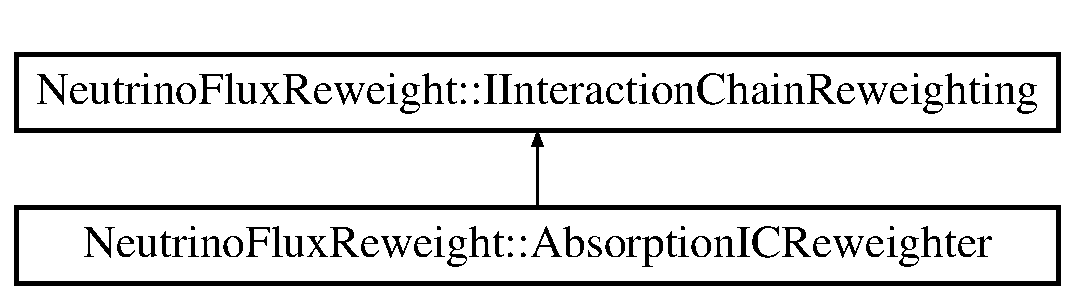
\includegraphics[height=2.000000cm]{class_neutrino_flux_reweight_1_1_absorption_i_c_reweighter}
\end{center}
\end{figure}
\subsection*{Public Member Functions}
\begin{DoxyCompactItemize}
\item 
\hyperlink{class_neutrino_flux_reweight_1_1_absorption_i_c_reweighter_a16ce26791334162b0a512667f93044fc}{Absorption\-I\-C\-Reweighter} (int iuniv, const \hyperlink{class_neutrino_flux_reweight_1_1_parameter_table}{Parameter\-Table} \&cv\-\_\-pars, const \hyperlink{class_neutrino_flux_reweight_1_1_parameter_table}{Parameter\-Table} \&univ\-\_\-pars)
\item 
virtual \hyperlink{class_neutrino_flux_reweight_1_1_absorption_i_c_reweighter_a2851345b01ad24a57576a7d6e1c32da0}{$\sim$\-Absorption\-I\-C\-Reweighter} ()
\item 
virtual std\-::vector$<$ bool $>$ \hyperlink{class_neutrino_flux_reweight_1_1_absorption_i_c_reweighter_adb94609e23ec8ee9123abf30d52fae40}{can\-Reweight} (const \hyperlink{class_neutrino_flux_reweight_1_1_interaction_chain_data}{Interaction\-Chain\-Data} \&aa)
\begin{DoxyCompactList}\small\item\em Look through the \hyperlink{class_neutrino_flux_reweight_1_1_interaction_chain_data}{Interaction\-Chain\-Data} input and identify those Interactions that can be reweighted as part of a chain. We return a vector indicating which elements will be assigned a weight by calculate\-Weight. \end{DoxyCompactList}\item 
virtual double \hyperlink{class_neutrino_flux_reweight_1_1_absorption_i_c_reweighter_a07104ede5adc45dfeda61fc90004bec3}{calculate\-Weight} (const \hyperlink{class_neutrino_flux_reweight_1_1_interaction_chain_data}{Interaction\-Chain\-Data} \&aa)
\begin{DoxyCompactList}\small\item\em calculate a weight for this interaction chain given the central value parameters and the parameters for this universe. The weight is something like\-: f(cv)/f(M\-C) $\ast$ f(univ)/f(cv) where cv in this case corresponds to the best value of the parameter, given the data. If univ\-\_\-pars=cv\-\_\-pars then we are calculating a central value weight. Note, \hyperlink{class_neutrino_flux_reweight_1_1_absorption_i_c_reweighter_adb94609e23ec8ee9123abf30d52fae40}{can\-Reweight()} should be called to determine which elements of the chain are covered by the weight returned by \hyperlink{class_neutrino_flux_reweight_1_1_absorption_i_c_reweighter_a07104ede5adc45dfeda61fc90004bec3}{calculate\-Weight()} \end{DoxyCompactList}\end{DoxyCompactItemize}
\subsection*{Public Attributes}
\begin{DoxyCompactItemize}
\item 
const \hyperlink{class_neutrino_flux_reweight_1_1_parameter_table}{Parameter\-Table} \& \hyperlink{class_neutrino_flux_reweight_1_1_absorption_i_c_reweighter_a48bef225244e591385f084f20ce4c267}{cv\-Pars}
\item 
const \hyperlink{class_neutrino_flux_reweight_1_1_parameter_table}{Parameter\-Table} \& \hyperlink{class_neutrino_flux_reweight_1_1_absorption_i_c_reweighter_a76db51ee33303841ac96b51a71d9e193}{univ\-Pars}
\end{DoxyCompactItemize}
\subsection*{Private Attributes}
\begin{DoxyCompactItemize}
\item 
int \hyperlink{class_neutrino_flux_reweight_1_1_absorption_i_c_reweighter_a634755f48664f8b84b036b068a543ac5}{i\-Univ}
\item 
float \hyperlink{class_neutrino_flux_reweight_1_1_absorption_i_c_reweighter_a9eb43d6dc37d7d56c5fc63ef04ae0b95}{inel\-\_\-pi\-Al\-\_\-xsec}
\item 
float \hyperlink{class_neutrino_flux_reweight_1_1_absorption_i_c_reweighter_ada87b802b0f5a66ffbdae8557c677857}{inel\-\_\-kap\-Al\-\_\-xsec\-\_\-low\-P}
\item 
float \hyperlink{class_neutrino_flux_reweight_1_1_absorption_i_c_reweighter_a14274987e004a55f88767d9ec22d7c9d}{inel\-\_\-kap\-Al\-\_\-xsec\-\_\-high\-P}
\item 
float \hyperlink{class_neutrino_flux_reweight_1_1_absorption_i_c_reweighter_a0b3707268a0569123e3d7116d35d63d6}{inel\-\_\-kam\-Al\-\_\-xsec\-\_\-low\-P}
\item 
float \hyperlink{class_neutrino_flux_reweight_1_1_absorption_i_c_reweighter_a216cbaf9abd19f100ed5444b7a11011d}{inel\-\_\-kam\-Al\-\_\-xsec\-\_\-high\-P}
\end{DoxyCompactItemize}


\subsection{Detailed Description}


Definition at line 16 of file Absorption\-I\-C\-Reweighter.\-h.



\subsection{Constructor \& Destructor Documentation}
\hypertarget{class_neutrino_flux_reweight_1_1_absorption_i_c_reweighter_a16ce26791334162b0a512667f93044fc}{\index{Neutrino\-Flux\-Reweight\-::\-Absorption\-I\-C\-Reweighter@{Neutrino\-Flux\-Reweight\-::\-Absorption\-I\-C\-Reweighter}!Absorption\-I\-C\-Reweighter@{Absorption\-I\-C\-Reweighter}}
\index{Absorption\-I\-C\-Reweighter@{Absorption\-I\-C\-Reweighter}!NeutrinoFluxReweight::AbsorptionICReweighter@{Neutrino\-Flux\-Reweight\-::\-Absorption\-I\-C\-Reweighter}}
\subsubsection[{Absorption\-I\-C\-Reweighter}]{\setlength{\rightskip}{0pt plus 5cm}Neutrino\-Flux\-Reweight\-::\-Absorption\-I\-C\-Reweighter\-::\-Absorption\-I\-C\-Reweighter (
\begin{DoxyParamCaption}
\item[{int}]{iuniv, }
\item[{const {\bf Parameter\-Table} \&}]{cv\-\_\-pars, }
\item[{const {\bf Parameter\-Table} \&}]{univ\-\_\-pars}
\end{DoxyParamCaption}
)}}\label{class_neutrino_flux_reweight_1_1_absorption_i_c_reweighter_a16ce26791334162b0a512667f93044fc}
The constructor. Note, we pass central value and single universe parameters in this constructor only. There is thus a 1 to 1 correspondence between an instance of this class and a given universe. 

Definition at line 12 of file Absorption\-I\-C\-Reweighter.\-cpp.


\begin{DoxyCode}
12                                                                                                            
                    :\hyperlink{class_neutrino_flux_reweight_1_1_absorption_i_c_reweighter_a48bef225244e591385f084f20ce4c267}{cvPars}(cv\_pars),\hyperlink{class_neutrino_flux_reweight_1_1_absorption_i_c_reweighter_a76db51ee33303841ac96b51a71d9e193}{univPars}(univ\_pars),\hyperlink{class_neutrino_flux_reweight_1_1_absorption_i_c_reweighter_a634755f48664f8b84b036b068a543ac5}{iUniv}(iuniv)\{ 
13 
14     \textcolor{comment}{// const boost::interprocess::flat\_map<std::string, double>& dsig\_table = univPars.getMap();}
15     \hyperlink{class_neutrino_flux_reweight_1_1_absorption_i_c_reweighter_a9eb43d6dc37d7d56c5fc63ef04ae0b95}{inel\_piAl\_xsec} = \hyperlink{class_neutrino_flux_reweight_1_1_absorption_i_c_reweighter_a76db51ee33303841ac96b51a71d9e193}{univPars}.\hyperlink{class_neutrino_flux_reweight_1_1_parameter_table_acb7dc8335b65b116f6092f2fa57ca5ed}{getParameterValue}(\textcolor{stringliteral}{"inel\_piAl\_xsec"});
16     \hyperlink{class_neutrino_flux_reweight_1_1_absorption_i_c_reweighter_ada87b802b0f5a66ffbdae8557c677857}{inel\_kapAl\_xsec\_lowP}  = \hyperlink{class_neutrino_flux_reweight_1_1_absorption_i_c_reweighter_a76db51ee33303841ac96b51a71d9e193}{univPars}.
      \hyperlink{class_neutrino_flux_reweight_1_1_parameter_table_acb7dc8335b65b116f6092f2fa57ca5ed}{getParameterValue}(\textcolor{stringliteral}{"inel\_kapAl\_xsec\_lowP"});
17     \hyperlink{class_neutrino_flux_reweight_1_1_absorption_i_c_reweighter_a14274987e004a55f88767d9ec22d7c9d}{inel\_kapAl\_xsec\_highP} = \hyperlink{class_neutrino_flux_reweight_1_1_absorption_i_c_reweighter_a76db51ee33303841ac96b51a71d9e193}{univPars}.
      \hyperlink{class_neutrino_flux_reweight_1_1_parameter_table_acb7dc8335b65b116f6092f2fa57ca5ed}{getParameterValue}(\textcolor{stringliteral}{"inel\_kapAl\_xsec\_highP"});
18     \hyperlink{class_neutrino_flux_reweight_1_1_absorption_i_c_reweighter_a0b3707268a0569123e3d7116d35d63d6}{inel\_kamAl\_xsec\_lowP}  = \hyperlink{class_neutrino_flux_reweight_1_1_absorption_i_c_reweighter_a76db51ee33303841ac96b51a71d9e193}{univPars}.
      \hyperlink{class_neutrino_flux_reweight_1_1_parameter_table_acb7dc8335b65b116f6092f2fa57ca5ed}{getParameterValue}(\textcolor{stringliteral}{"inel\_kamAl\_xsec\_lowP"});
19     \hyperlink{class_neutrino_flux_reweight_1_1_absorption_i_c_reweighter_a216cbaf9abd19f100ed5444b7a11011d}{inel\_kamAl\_xsec\_highP} = \hyperlink{class_neutrino_flux_reweight_1_1_absorption_i_c_reweighter_a76db51ee33303841ac96b51a71d9e193}{univPars}.
      \hyperlink{class_neutrino_flux_reweight_1_1_parameter_table_acb7dc8335b65b116f6092f2fa57ca5ed}{getParameterValue}(\textcolor{stringliteral}{"inel\_kamAl\_xsec\_highP"});
20     
21   \}
\end{DoxyCode}
\hypertarget{class_neutrino_flux_reweight_1_1_absorption_i_c_reweighter_a2851345b01ad24a57576a7d6e1c32da0}{\index{Neutrino\-Flux\-Reweight\-::\-Absorption\-I\-C\-Reweighter@{Neutrino\-Flux\-Reweight\-::\-Absorption\-I\-C\-Reweighter}!$\sim$\-Absorption\-I\-C\-Reweighter@{$\sim$\-Absorption\-I\-C\-Reweighter}}
\index{$\sim$\-Absorption\-I\-C\-Reweighter@{$\sim$\-Absorption\-I\-C\-Reweighter}!NeutrinoFluxReweight::AbsorptionICReweighter@{Neutrino\-Flux\-Reweight\-::\-Absorption\-I\-C\-Reweighter}}
\subsubsection[{$\sim$\-Absorption\-I\-C\-Reweighter}]{\setlength{\rightskip}{0pt plus 5cm}Neutrino\-Flux\-Reweight\-::\-Absorption\-I\-C\-Reweighter\-::$\sim$\-Absorption\-I\-C\-Reweighter (
\begin{DoxyParamCaption}
{}
\end{DoxyParamCaption}
)\hspace{0.3cm}{\ttfamily [virtual]}}}\label{class_neutrino_flux_reweight_1_1_absorption_i_c_reweighter_a2851345b01ad24a57576a7d6e1c32da0}


Definition at line 22 of file Absorption\-I\-C\-Reweighter.\-cpp.


\begin{DoxyCode}
22                                                  \{
23     
24   \}
\end{DoxyCode}


\subsection{Member Function Documentation}
\hypertarget{class_neutrino_flux_reweight_1_1_absorption_i_c_reweighter_a07104ede5adc45dfeda61fc90004bec3}{\index{Neutrino\-Flux\-Reweight\-::\-Absorption\-I\-C\-Reweighter@{Neutrino\-Flux\-Reweight\-::\-Absorption\-I\-C\-Reweighter}!calculate\-Weight@{calculate\-Weight}}
\index{calculate\-Weight@{calculate\-Weight}!NeutrinoFluxReweight::AbsorptionICReweighter@{Neutrino\-Flux\-Reweight\-::\-Absorption\-I\-C\-Reweighter}}
\subsubsection[{calculate\-Weight}]{\setlength{\rightskip}{0pt plus 5cm}double Neutrino\-Flux\-Reweight\-::\-Absorption\-I\-C\-Reweighter\-::calculate\-Weight (
\begin{DoxyParamCaption}
\item[{const {\bf Interaction\-Chain\-Data} \&}]{aa}
\end{DoxyParamCaption}
)\hspace{0.3cm}{\ttfamily [virtual]}}}\label{class_neutrino_flux_reweight_1_1_absorption_i_c_reweighter_a07104ede5adc45dfeda61fc90004bec3}


calculate a weight for this interaction chain given the central value parameters and the parameters for this universe. The weight is something like\-: f(cv)/f(M\-C) $\ast$ f(univ)/f(cv) where cv in this case corresponds to the best value of the parameter, given the data. If univ\-\_\-pars=cv\-\_\-pars then we are calculating a central value weight. Note, \hyperlink{class_neutrino_flux_reweight_1_1_absorption_i_c_reweighter_adb94609e23ec8ee9123abf30d52fae40}{can\-Reweight()} should be called to determine which elements of the chain are covered by the weight returned by \hyperlink{class_neutrino_flux_reweight_1_1_absorption_i_c_reweighter_a07104ede5adc45dfeda61fc90004bec3}{calculate\-Weight()} 



Implements \hyperlink{class_neutrino_flux_reweight_1_1_i_interaction_chain_reweighting_ae28403553637013fdc720674ee24c7c5}{Neutrino\-Flux\-Reweight\-::\-I\-Interaction\-Chain\-Reweighting}.



Definition at line 42 of file Absorption\-I\-C\-Reweighter.\-cpp.


\begin{DoxyCode}
42                                                                               \{
43      
44     std::vector<ParticlesThroughVolumesData>  vec\_ptv = aa.ptv\_info;
45     std::string namepar;
46     \textcolor{comment}{// document how this number was computed}
47     \textcolor{keywordtype}{double} NA\_mb    = 6.02E-4; \textcolor{comment}{// conversion factor to get tot\_dist below into unitless numbers}
48     \textcolor{keywordtype}{double} wgt      = 1.0;
49     \textcolor{keywordtype}{double} tot\_dist = 0.0;
50     \textcolor{keywordtype}{double} low\_val  = 1.E-20;   
51     \textcolor{keywordtype}{int} index\_vol = 0;
52     
53     \textcolor{comment}{// need to document}
54     \textcolor{keywordflow}{for}(\textcolor{keywordtype}{int} ii=0;ii<3;ii++)\{
55       \textcolor{keywordtype}{float} shift = 0.0;
56       tot\_dist = vec\_ptv[index\_vol].AmountMat[ii];
57       \textcolor{keywordflow}{if}(tot\_dist<low\_val)\textcolor{keywordflow}{continue};
58       \textcolor{keywordflow}{if}(abs(vec\_ptv[index\_vol].Pdgs[ii])!=321 && abs(vec\_ptv[index\_vol].Pdgs[ii])!=211)\textcolor{keywordflow}{continue};
59       
60       \textcolor{keywordflow}{if}(abs(vec\_ptv[index\_vol].Pdgs[ii])== 211)shift = \hyperlink{class_neutrino_flux_reweight_1_1_absorption_i_c_reweighter_a9eb43d6dc37d7d56c5fc63ef04ae0b95}{inel\_piAl\_xsec};
61       \textcolor{keywordflow}{else} \textcolor{keywordflow}{if}(vec\_ptv[index\_vol].Pdgs[ii]== 321 && vec\_ptv[index\_vol].Moms[ii]<2.0)shift = 
      \hyperlink{class_neutrino_flux_reweight_1_1_absorption_i_c_reweighter_ada87b802b0f5a66ffbdae8557c677857}{inel\_kapAl\_xsec\_lowP};
62       \textcolor{keywordflow}{else} \textcolor{keywordflow}{if}(vec\_ptv[index\_vol].Pdgs[ii]== 321 && vec\_ptv[index\_vol].Moms[ii]>2.0)shift = 
      \hyperlink{class_neutrino_flux_reweight_1_1_absorption_i_c_reweighter_a14274987e004a55f88767d9ec22d7c9d}{inel\_kapAl\_xsec\_highP};
63       \textcolor{keywordflow}{else} \textcolor{keywordflow}{if}(vec\_ptv[index\_vol].Pdgs[ii]==-321 && vec\_ptv[index\_vol].Moms[ii]<2.0)shift = 
      \hyperlink{class_neutrino_flux_reweight_1_1_absorption_i_c_reweighter_a0b3707268a0569123e3d7116d35d63d6}{inel\_kamAl\_xsec\_lowP};
64       \textcolor{keywordflow}{else} \textcolor{keywordflow}{if}(vec\_ptv[index\_vol].Pdgs[ii]==-321 && vec\_ptv[index\_vol].Moms[ii]>2.0)shift = 
      \hyperlink{class_neutrino_flux_reweight_1_1_absorption_i_c_reweighter_a216cbaf9abd19f100ed5444b7a11011d}{inel\_kamAl\_xsec\_highP};
65       \textcolor{comment}{// converts tot\_dist into a unitless number and applies MU shift}
66       tot\_dist *= NA\_mb;
67       tot\_dist *= shift;
68       
69       wgt *= exp(-1.0*tot\_dist);   
70     \}
71     
72     \textcolor{keywordflow}{return} wgt;
73     
74   \}
\end{DoxyCode}
\hypertarget{class_neutrino_flux_reweight_1_1_absorption_i_c_reweighter_adb94609e23ec8ee9123abf30d52fae40}{\index{Neutrino\-Flux\-Reweight\-::\-Absorption\-I\-C\-Reweighter@{Neutrino\-Flux\-Reweight\-::\-Absorption\-I\-C\-Reweighter}!can\-Reweight@{can\-Reweight}}
\index{can\-Reweight@{can\-Reweight}!NeutrinoFluxReweight::AbsorptionICReweighter@{Neutrino\-Flux\-Reweight\-::\-Absorption\-I\-C\-Reweighter}}
\subsubsection[{can\-Reweight}]{\setlength{\rightskip}{0pt plus 5cm}std\-::vector$<$ bool $>$ Neutrino\-Flux\-Reweight\-::\-Absorption\-I\-C\-Reweighter\-::can\-Reweight (
\begin{DoxyParamCaption}
\item[{const {\bf Interaction\-Chain\-Data} \&}]{aa}
\end{DoxyParamCaption}
)\hspace{0.3cm}{\ttfamily [virtual]}}}\label{class_neutrino_flux_reweight_1_1_absorption_i_c_reweighter_adb94609e23ec8ee9123abf30d52fae40}


Look through the \hyperlink{class_neutrino_flux_reweight_1_1_interaction_chain_data}{Interaction\-Chain\-Data} input and identify those Interactions that can be reweighted as part of a chain. We return a vector indicating which elements will be assigned a weight by calculate\-Weight. 



Implements \hyperlink{class_neutrino_flux_reweight_1_1_i_interaction_chain_reweighting_aacf17580c1d316f0ebcdfdff7418e9e3}{Neutrino\-Flux\-Reweight\-::\-I\-Interaction\-Chain\-Reweighting}.



Definition at line 25 of file Absorption\-I\-C\-Reweighter.\-cpp.


\begin{DoxyCode}
25                                                                                    \{
26  
27     std::vector<bool> this\_nodes;
28     \textcolor{keywordtype}{int} index\_vol = 0;
29     \textcolor{keywordtype}{double} low\_val = 1.E-20;    
30   
31     std::vector<ParticlesThroughVolumesData>  vec\_ptv = aa.ptv\_info;
32 
33     \textcolor{keywordtype}{bool} passVOL = \textcolor{keyword}{false};
34     \textcolor{comment}{//Cheking at least one ancestor with amount of materail value:}
35     \textcolor{keywordflow}{for}(\textcolor{keywordtype}{int} ii=0;ii<3;ii++)\{
36       passVOL = passVOL || (vec\_ptv[index\_vol].AmountMat[ii] >low\_val && (abs(vec\_ptv[index\_vol].Pdgs[ii])=
      =211 || abs(vec\_ptv[index\_vol].Pdgs[ii])==321));
37     \}
38     this\_nodes.push\_back(passVOL);
39     \textcolor{keywordflow}{return} this\_nodes;
40 
41   \}
\end{DoxyCode}


\subsection{Member Data Documentation}
\hypertarget{class_neutrino_flux_reweight_1_1_absorption_i_c_reweighter_a48bef225244e591385f084f20ce4c267}{\index{Neutrino\-Flux\-Reweight\-::\-Absorption\-I\-C\-Reweighter@{Neutrino\-Flux\-Reweight\-::\-Absorption\-I\-C\-Reweighter}!cv\-Pars@{cv\-Pars}}
\index{cv\-Pars@{cv\-Pars}!NeutrinoFluxReweight::AbsorptionICReweighter@{Neutrino\-Flux\-Reweight\-::\-Absorption\-I\-C\-Reweighter}}
\subsubsection[{cv\-Pars}]{\setlength{\rightskip}{0pt plus 5cm}const {\bf Parameter\-Table}\& Neutrino\-Flux\-Reweight\-::\-Absorption\-I\-C\-Reweighter\-::cv\-Pars}}\label{class_neutrino_flux_reweight_1_1_absorption_i_c_reweighter_a48bef225244e591385f084f20ce4c267}


Definition at line 27 of file Absorption\-I\-C\-Reweighter.\-h.

\hypertarget{class_neutrino_flux_reweight_1_1_absorption_i_c_reweighter_a216cbaf9abd19f100ed5444b7a11011d}{\index{Neutrino\-Flux\-Reweight\-::\-Absorption\-I\-C\-Reweighter@{Neutrino\-Flux\-Reweight\-::\-Absorption\-I\-C\-Reweighter}!inel\-\_\-kam\-Al\-\_\-xsec\-\_\-high\-P@{inel\-\_\-kam\-Al\-\_\-xsec\-\_\-high\-P}}
\index{inel\-\_\-kam\-Al\-\_\-xsec\-\_\-high\-P@{inel\-\_\-kam\-Al\-\_\-xsec\-\_\-high\-P}!NeutrinoFluxReweight::AbsorptionICReweighter@{Neutrino\-Flux\-Reweight\-::\-Absorption\-I\-C\-Reweighter}}
\subsubsection[{inel\-\_\-kam\-Al\-\_\-xsec\-\_\-high\-P}]{\setlength{\rightskip}{0pt plus 5cm}float Neutrino\-Flux\-Reweight\-::\-Absorption\-I\-C\-Reweighter\-::inel\-\_\-kam\-Al\-\_\-xsec\-\_\-high\-P\hspace{0.3cm}{\ttfamily [private]}}}\label{class_neutrino_flux_reweight_1_1_absorption_i_c_reweighter_a216cbaf9abd19f100ed5444b7a11011d}


Definition at line 33 of file Absorption\-I\-C\-Reweighter.\-h.

\hypertarget{class_neutrino_flux_reweight_1_1_absorption_i_c_reweighter_a0b3707268a0569123e3d7116d35d63d6}{\index{Neutrino\-Flux\-Reweight\-::\-Absorption\-I\-C\-Reweighter@{Neutrino\-Flux\-Reweight\-::\-Absorption\-I\-C\-Reweighter}!inel\-\_\-kam\-Al\-\_\-xsec\-\_\-low\-P@{inel\-\_\-kam\-Al\-\_\-xsec\-\_\-low\-P}}
\index{inel\-\_\-kam\-Al\-\_\-xsec\-\_\-low\-P@{inel\-\_\-kam\-Al\-\_\-xsec\-\_\-low\-P}!NeutrinoFluxReweight::AbsorptionICReweighter@{Neutrino\-Flux\-Reweight\-::\-Absorption\-I\-C\-Reweighter}}
\subsubsection[{inel\-\_\-kam\-Al\-\_\-xsec\-\_\-low\-P}]{\setlength{\rightskip}{0pt plus 5cm}float Neutrino\-Flux\-Reweight\-::\-Absorption\-I\-C\-Reweighter\-::inel\-\_\-kam\-Al\-\_\-xsec\-\_\-low\-P\hspace{0.3cm}{\ttfamily [private]}}}\label{class_neutrino_flux_reweight_1_1_absorption_i_c_reweighter_a0b3707268a0569123e3d7116d35d63d6}


Definition at line 33 of file Absorption\-I\-C\-Reweighter.\-h.

\hypertarget{class_neutrino_flux_reweight_1_1_absorption_i_c_reweighter_a14274987e004a55f88767d9ec22d7c9d}{\index{Neutrino\-Flux\-Reweight\-::\-Absorption\-I\-C\-Reweighter@{Neutrino\-Flux\-Reweight\-::\-Absorption\-I\-C\-Reweighter}!inel\-\_\-kap\-Al\-\_\-xsec\-\_\-high\-P@{inel\-\_\-kap\-Al\-\_\-xsec\-\_\-high\-P}}
\index{inel\-\_\-kap\-Al\-\_\-xsec\-\_\-high\-P@{inel\-\_\-kap\-Al\-\_\-xsec\-\_\-high\-P}!NeutrinoFluxReweight::AbsorptionICReweighter@{Neutrino\-Flux\-Reweight\-::\-Absorption\-I\-C\-Reweighter}}
\subsubsection[{inel\-\_\-kap\-Al\-\_\-xsec\-\_\-high\-P}]{\setlength{\rightskip}{0pt plus 5cm}float Neutrino\-Flux\-Reweight\-::\-Absorption\-I\-C\-Reweighter\-::inel\-\_\-kap\-Al\-\_\-xsec\-\_\-high\-P\hspace{0.3cm}{\ttfamily [private]}}}\label{class_neutrino_flux_reweight_1_1_absorption_i_c_reweighter_a14274987e004a55f88767d9ec22d7c9d}


Definition at line 32 of file Absorption\-I\-C\-Reweighter.\-h.

\hypertarget{class_neutrino_flux_reweight_1_1_absorption_i_c_reweighter_ada87b802b0f5a66ffbdae8557c677857}{\index{Neutrino\-Flux\-Reweight\-::\-Absorption\-I\-C\-Reweighter@{Neutrino\-Flux\-Reweight\-::\-Absorption\-I\-C\-Reweighter}!inel\-\_\-kap\-Al\-\_\-xsec\-\_\-low\-P@{inel\-\_\-kap\-Al\-\_\-xsec\-\_\-low\-P}}
\index{inel\-\_\-kap\-Al\-\_\-xsec\-\_\-low\-P@{inel\-\_\-kap\-Al\-\_\-xsec\-\_\-low\-P}!NeutrinoFluxReweight::AbsorptionICReweighter@{Neutrino\-Flux\-Reweight\-::\-Absorption\-I\-C\-Reweighter}}
\subsubsection[{inel\-\_\-kap\-Al\-\_\-xsec\-\_\-low\-P}]{\setlength{\rightskip}{0pt plus 5cm}float Neutrino\-Flux\-Reweight\-::\-Absorption\-I\-C\-Reweighter\-::inel\-\_\-kap\-Al\-\_\-xsec\-\_\-low\-P\hspace{0.3cm}{\ttfamily [private]}}}\label{class_neutrino_flux_reweight_1_1_absorption_i_c_reweighter_ada87b802b0f5a66ffbdae8557c677857}


Definition at line 32 of file Absorption\-I\-C\-Reweighter.\-h.

\hypertarget{class_neutrino_flux_reweight_1_1_absorption_i_c_reweighter_a9eb43d6dc37d7d56c5fc63ef04ae0b95}{\index{Neutrino\-Flux\-Reweight\-::\-Absorption\-I\-C\-Reweighter@{Neutrino\-Flux\-Reweight\-::\-Absorption\-I\-C\-Reweighter}!inel\-\_\-pi\-Al\-\_\-xsec@{inel\-\_\-pi\-Al\-\_\-xsec}}
\index{inel\-\_\-pi\-Al\-\_\-xsec@{inel\-\_\-pi\-Al\-\_\-xsec}!NeutrinoFluxReweight::AbsorptionICReweighter@{Neutrino\-Flux\-Reweight\-::\-Absorption\-I\-C\-Reweighter}}
\subsubsection[{inel\-\_\-pi\-Al\-\_\-xsec}]{\setlength{\rightskip}{0pt plus 5cm}float Neutrino\-Flux\-Reweight\-::\-Absorption\-I\-C\-Reweighter\-::inel\-\_\-pi\-Al\-\_\-xsec\hspace{0.3cm}{\ttfamily [private]}}}\label{class_neutrino_flux_reweight_1_1_absorption_i_c_reweighter_a9eb43d6dc37d7d56c5fc63ef04ae0b95}


Definition at line 31 of file Absorption\-I\-C\-Reweighter.\-h.

\hypertarget{class_neutrino_flux_reweight_1_1_absorption_i_c_reweighter_a634755f48664f8b84b036b068a543ac5}{\index{Neutrino\-Flux\-Reweight\-::\-Absorption\-I\-C\-Reweighter@{Neutrino\-Flux\-Reweight\-::\-Absorption\-I\-C\-Reweighter}!i\-Univ@{i\-Univ}}
\index{i\-Univ@{i\-Univ}!NeutrinoFluxReweight::AbsorptionICReweighter@{Neutrino\-Flux\-Reweight\-::\-Absorption\-I\-C\-Reweighter}}
\subsubsection[{i\-Univ}]{\setlength{\rightskip}{0pt plus 5cm}int Neutrino\-Flux\-Reweight\-::\-Absorption\-I\-C\-Reweighter\-::i\-Univ\hspace{0.3cm}{\ttfamily [private]}}}\label{class_neutrino_flux_reweight_1_1_absorption_i_c_reweighter_a634755f48664f8b84b036b068a543ac5}


Definition at line 30 of file Absorption\-I\-C\-Reweighter.\-h.

\hypertarget{class_neutrino_flux_reweight_1_1_absorption_i_c_reweighter_a76db51ee33303841ac96b51a71d9e193}{\index{Neutrino\-Flux\-Reweight\-::\-Absorption\-I\-C\-Reweighter@{Neutrino\-Flux\-Reweight\-::\-Absorption\-I\-C\-Reweighter}!univ\-Pars@{univ\-Pars}}
\index{univ\-Pars@{univ\-Pars}!NeutrinoFluxReweight::AbsorptionICReweighter@{Neutrino\-Flux\-Reweight\-::\-Absorption\-I\-C\-Reweighter}}
\subsubsection[{univ\-Pars}]{\setlength{\rightskip}{0pt plus 5cm}const {\bf Parameter\-Table}\& Neutrino\-Flux\-Reweight\-::\-Absorption\-I\-C\-Reweighter\-::univ\-Pars}}\label{class_neutrino_flux_reweight_1_1_absorption_i_c_reweighter_a76db51ee33303841ac96b51a71d9e193}


Definition at line 28 of file Absorption\-I\-C\-Reweighter.\-h.



The documentation for this class was generated from the following files\-:\begin{DoxyCompactItemize}
\item 
include/\hyperlink{_absorption_i_c_reweighter_8h}{Absorption\-I\-C\-Reweighter.\-h}\item 
src/\hyperlink{_absorption_i_c_reweighter_8cpp}{Absorption\-I\-C\-Reweighter.\-cpp}\end{DoxyCompactItemize}

\hypertarget{class_absorption_reweighter}{\section{Absorption\-Reweighter Class Reference}
\label{class_absorption_reweighter}\index{Absorption\-Reweighter@{Absorption\-Reweighter}}
}


Reweight a M\-C survival probabiity when the particles through volumes.  




{\ttfamily \#include $<$Absorption\-I\-C\-Reweighter.\-h$>$}



\subsection{Detailed Description}
Reweight a M\-C survival probabiity when the particles through volumes. 

The documentation for this class was generated from the following file\-:\begin{DoxyCompactItemize}
\item 
include/\hyperlink{_absorption_i_c_reweighter_8h}{Absorption\-I\-C\-Reweighter.\-h}\end{DoxyCompactItemize}

\hypertarget{class_absorption_reweighter}{\section{Absorption\-Reweighter Class Reference}
\label{class_absorption_reweighter}\index{Absorption\-Reweighter@{Absorption\-Reweighter}}
}


Reweight a M\-C survival probabiity when the particles through volumes.  




{\ttfamily \#include $<$Absorption\-I\-C\-Reweighter.\-h$>$}



\subsection{Detailed Description}
Reweight a M\-C survival probabiity when the particles through volumes. 

The documentation for this class was generated from the following file\-:\begin{DoxyCompactItemize}
\item 
include/\hyperlink{_absorption_i_c_reweighter_8h}{Absorption\-I\-C\-Reweighter.\-h}\end{DoxyCompactItemize}

\hypertarget{class_absorption_reweighter}{\section{Absorption\-Reweighter Class Reference}
\label{class_absorption_reweighter}\index{Absorption\-Reweighter@{Absorption\-Reweighter}}
}


Reweight a M\-C survival probabiity when the particles through volumes.  




{\ttfamily \#include $<$Absorption\-I\-C\-Reweighter.\-h$>$}



\subsection{Detailed Description}
Reweight a M\-C survival probabiity when the particles through volumes. 

The documentation for this class was generated from the following file\-:\begin{DoxyCompactItemize}
\item 
include/\hyperlink{_absorption_i_c_reweighter_8h}{Absorption\-I\-C\-Reweighter.\-h}\end{DoxyCompactItemize}

\hypertarget{class_neutrino_flux_reweight_1_1_attenuation_m_c}{\section{Neutrino\-Flux\-Reweight\-:\-:Attenuation\-M\-C Class Reference}
\label{class_neutrino_flux_reweight_1_1_attenuation_m_c}\index{Neutrino\-Flux\-Reweight\-::\-Attenuation\-M\-C@{Neutrino\-Flux\-Reweight\-::\-Attenuation\-M\-C}}
}


{\ttfamily \#include $<$Attenuation\-M\-C.\-h$>$}

\subsection*{Static Public Member Functions}
\begin{DoxyCompactItemize}
\item 
static \hyperlink{class_neutrino_flux_reweight_1_1_attenuation_m_c}{Attenuation\-M\-C} $\ast$ \hyperlink{class_neutrino_flux_reweight_1_1_attenuation_m_c_acc338217e771bf334014ed943015e6a1}{get\-Instance} ()
\end{DoxyCompactItemize}
\subsection*{Public Attributes}
\begin{DoxyCompactItemize}
\item 
T\-H1\-D $\ast$ \hyperlink{class_neutrino_flux_reweight_1_1_attenuation_m_c_a7a9edf7fb1e5af0611eacfaba7d63879}{h\-X\-S\-\_\-pi\-Al}
\item 
T\-H1\-D $\ast$ \hyperlink{class_neutrino_flux_reweight_1_1_attenuation_m_c_a6a8883254ecc6e301643493923c3cde0}{h\-X\-S\-\_\-prt\-C}
\item 
T\-H1\-D $\ast$ \hyperlink{class_neutrino_flux_reweight_1_1_attenuation_m_c_aa7f4bb3745202fd3a48fb9e295317219}{h\-X\-S\-\_\-pi\-C}
\item 
T\-H1\-D $\ast$ \hyperlink{class_neutrino_flux_reweight_1_1_attenuation_m_c_afe67d35bfdea4d6b91bd6b16f7404bb2}{h\-X\-S\-\_\-kap\-C}
\item 
T\-H1\-D $\ast$ \hyperlink{class_neutrino_flux_reweight_1_1_attenuation_m_c_a89dfdfa2e55926db7bdc4ec685e0003e}{h\-X\-S\-\_\-kam\-C}
\item 
std\-::vector$<$ T\-H1\-D $\ast$ $>$ \hyperlink{class_neutrino_flux_reweight_1_1_attenuation_m_c_a96f19a370160ceee2c8bf61d93a34085}{hzpostgt\-\_\-pip\-\_\-le}
\item 
std\-::vector$<$ T\-H1\-D $\ast$ $>$ \hyperlink{class_neutrino_flux_reweight_1_1_attenuation_m_c_a4a4fe98dd8c926d1996b1bcf492b65cd}{hzpostgt\-\_\-pip\-\_\-me}
\item 
std\-::vector$<$ T\-H1\-D $\ast$ $>$ \hyperlink{class_neutrino_flux_reweight_1_1_attenuation_m_c_a8e2000306243ba7ee0e93814ded1c964}{hzpostgt\-\_\-pim\-\_\-le}
\item 
std\-::vector$<$ T\-H1\-D $\ast$ $>$ \hyperlink{class_neutrino_flux_reweight_1_1_attenuation_m_c_ada00bc8840f8c94bdf92796e7c87b103}{hzpostgt\-\_\-pim\-\_\-me}
\item 
std\-::vector$<$ T\-H1\-D $\ast$ $>$ \hyperlink{class_neutrino_flux_reweight_1_1_attenuation_m_c_aa62930aa4128449906cd2b661a063355}{hzpostgt\-\_\-kap\-\_\-le}
\item 
std\-::vector$<$ T\-H1\-D $\ast$ $>$ \hyperlink{class_neutrino_flux_reweight_1_1_attenuation_m_c_aec1b443980cc76c016d34149707d0961}{hzpostgt\-\_\-kap\-\_\-me}
\item 
std\-::vector$<$ T\-H1\-D $\ast$ $>$ \hyperlink{class_neutrino_flux_reweight_1_1_attenuation_m_c_af7f31787553e49e1803626c24e722277}{hzpostgt\-\_\-kam\-\_\-le}
\item 
std\-::vector$<$ T\-H1\-D $\ast$ $>$ \hyperlink{class_neutrino_flux_reweight_1_1_attenuation_m_c_ace0dd74d05ab00993b319e53087f2ce2}{hzpostgt\-\_\-kam\-\_\-me}
\end{DoxyCompactItemize}
\subsection*{Private Member Functions}
\begin{DoxyCompactItemize}
\item 
\hyperlink{class_neutrino_flux_reweight_1_1_attenuation_m_c_a53038aecee97225821a39b29f59dde79}{Attenuation\-M\-C} ()
\item 
\hyperlink{class_neutrino_flux_reweight_1_1_attenuation_m_c_ae87eeab4f056bf9fae23433d879ff5c0}{$\sim$\-Attenuation\-M\-C} ()
\end{DoxyCompactItemize}
\subsection*{Private Attributes}
\begin{DoxyCompactItemize}
\item 
T\-File $\ast$ \hyperlink{class_neutrino_flux_reweight_1_1_attenuation_m_c_a5c8c620e955ec534263d78013c1c086a}{f\-Inel\-X\-S\-\_\-\-M\-C}
\item 
T\-File $\ast$ \hyperlink{class_neutrino_flux_reweight_1_1_attenuation_m_c_a66fcb5745e72eda64f9081b5b0ef4399}{fzpos\-\_\-tgt\-\_\-\-M\-C\-\_\-le}
\item 
T\-File $\ast$ \hyperlink{class_neutrino_flux_reweight_1_1_attenuation_m_c_a93e5ae3f1982c3dddd6c57ea47e230ea}{fzpos\-\_\-tgt\-\_\-\-M\-C\-\_\-me}
\end{DoxyCompactItemize}
\subsection*{Static Private Attributes}
\begin{DoxyCompactItemize}
\item 
static \hyperlink{class_neutrino_flux_reweight_1_1_attenuation_m_c}{Attenuation\-M\-C} $\ast$ \hyperlink{class_neutrino_flux_reweight_1_1_attenuation_m_c_ab75129542683e731060a5911a27e93fc}{instance} = 0
\end{DoxyCompactItemize}


\subsection{Detailed Description}


Definition at line 11 of file Attenuation\-M\-C.\-h.



\subsection{Constructor \& Destructor Documentation}
\hypertarget{class_neutrino_flux_reweight_1_1_attenuation_m_c_a53038aecee97225821a39b29f59dde79}{\index{Neutrino\-Flux\-Reweight\-::\-Attenuation\-M\-C@{Neutrino\-Flux\-Reweight\-::\-Attenuation\-M\-C}!Attenuation\-M\-C@{Attenuation\-M\-C}}
\index{Attenuation\-M\-C@{Attenuation\-M\-C}!NeutrinoFluxReweight::AttenuationMC@{Neutrino\-Flux\-Reweight\-::\-Attenuation\-M\-C}}
\subsubsection[{Attenuation\-M\-C}]{\setlength{\rightskip}{0pt plus 5cm}Neutrino\-Flux\-Reweight\-::\-Attenuation\-M\-C\-::\-Attenuation\-M\-C (
\begin{DoxyParamCaption}
{}
\end{DoxyParamCaption}
)\hspace{0.3cm}{\ttfamily [private]}}}\label{class_neutrino_flux_reweight_1_1_attenuation_m_c_a53038aecee97225821a39b29f59dde79}


Definition at line 9 of file Attenuation\-M\-C.\-cpp.


\begin{DoxyCode}
9                               \{
10     \textcolor{keyword}{const} \textcolor{keywordtype}{char}* ppfxDir = getenv(\textcolor{stringliteral}{"PPFX\_DIR"});
11     \textcolor{keywordtype}{char} dirData[400]; 
12     sprintf(dirData,\textcolor{stringliteral}{"%s/data"},ppfxDir);
13 
14     \hyperlink{class_neutrino_flux_reweight_1_1_attenuation_m_c_a5c8c620e955ec534263d78013c1c086a}{AttenuationMC::fInelXS\_MC} = \textcolor{keyword}{new} TFile(Form(\textcolor{stringliteral}{"%s/MC/InelXS\_geant4.root"},dirData)
      ,\textcolor{stringliteral}{"read"});
15 
16     \hyperlink{class_neutrino_flux_reweight_1_1_attenuation_m_c_a66fcb5745e72eda64f9081b5b0ef4399}{AttenuationMC::fzpos\_tgt\_MC\_le} = \textcolor{keyword}{new} TFile(Form(\textcolor{stringliteral}{"
      %s/MIPP/tarpos\_yield\_le.root"},dirData),\textcolor{stringliteral}{"read"});
17     \hyperlink{class_neutrino_flux_reweight_1_1_attenuation_m_c_a93e5ae3f1982c3dddd6c57ea47e230ea}{AttenuationMC::fzpos\_tgt\_MC\_me} = \textcolor{keyword}{new} TFile(Form(\textcolor{stringliteral}{"
      %s/MIPP/tarpos\_yield\_me.root"},dirData),\textcolor{stringliteral}{"read"});
18     
19     \textcolor{comment}{//Loading the geant4 inelastic cross section for pion on Aluminum}
20     \hyperlink{class_neutrino_flux_reweight_1_1_attenuation_m_c_a7a9edf7fb1e5af0611eacfaba7d63879}{AttenuationMC::hXS\_piAl}  = (TH1D*)
      \hyperlink{class_neutrino_flux_reweight_1_1_attenuation_m_c_a5c8c620e955ec534263d78013c1c086a}{AttenuationMC::fInelXS\_MC}->Get(\textcolor{stringliteral}{"pip/hpip\_Al"});
21     \hyperlink{class_neutrino_flux_reweight_1_1_attenuation_m_c_a6a8883254ecc6e301643493923c3cde0}{AttenuationMC::hXS\_prtC}  = (TH1D*)
      \hyperlink{class_neutrino_flux_reweight_1_1_attenuation_m_c_a5c8c620e955ec534263d78013c1c086a}{AttenuationMC::fInelXS\_MC}->Get(\textcolor{stringliteral}{"prt/hprt\_C"});
22     \hyperlink{class_neutrino_flux_reweight_1_1_attenuation_m_c_aa7f4bb3745202fd3a48fb9e295317219}{AttenuationMC::hXS\_piC}   = (TH1D*)
      \hyperlink{class_neutrino_flux_reweight_1_1_attenuation_m_c_a5c8c620e955ec534263d78013c1c086a}{AttenuationMC::fInelXS\_MC}->Get(\textcolor{stringliteral}{"pip/hpip\_C"});
23     \hyperlink{class_neutrino_flux_reweight_1_1_attenuation_m_c_afe67d35bfdea4d6b91bd6b16f7404bb2}{AttenuationMC::hXS\_kapC}  = (TH1D*)
      \hyperlink{class_neutrino_flux_reweight_1_1_attenuation_m_c_a5c8c620e955ec534263d78013c1c086a}{AttenuationMC::fInelXS\_MC}->Get(\textcolor{stringliteral}{"kap/hkap\_C"});
24     \hyperlink{class_neutrino_flux_reweight_1_1_attenuation_m_c_a89dfdfa2e55926db7bdc4ec685e0003e}{AttenuationMC::hXS\_kamC}  = (TH1D*)
      \hyperlink{class_neutrino_flux_reweight_1_1_attenuation_m_c_a5c8c620e955ec534263d78013c1c086a}{AttenuationMC::fInelXS\_MC}->Get(\textcolor{stringliteral}{"kam/hkam\_C"});
25     
26     \textcolor{comment}{//Loading z postition histograms from MC g4NuMI:}
27     \textcolor{comment}{//These are yields per z position per MIPP particle per MIPP bin.}
28     \textcolor{comment}{//per 2.5E8 POT}
29     \textcolor{comment}{//For pip: 124 bins, for pim: 119}
30     \textcolor{keywordtype}{char} namehist[100];
31     \textcolor{keywordflow}{for}(\textcolor{keywordtype}{int} ibin=0;ibin<124;ibin++)\{
32       sprintf(namehist,\textcolor{stringliteral}{"pip/htar\_ydz\_pip\_bin%d"},ibin);
33       \hyperlink{class_neutrino_flux_reweight_1_1_attenuation_m_c_a96f19a370160ceee2c8bf61d93a34085}{AttenuationMC::hzpostgt\_pip\_le}.push\_back((TH1D*)
      \hyperlink{class_neutrino_flux_reweight_1_1_attenuation_m_c_a66fcb5745e72eda64f9081b5b0ef4399}{AttenuationMC::fzpos\_tgt\_MC\_le}->Get(namehist));
34       \hyperlink{class_neutrino_flux_reweight_1_1_attenuation_m_c_a4a4fe98dd8c926d1996b1bcf492b65cd}{AttenuationMC::hzpostgt\_pip\_me}.push\_back((TH1D*)
      \hyperlink{class_neutrino_flux_reweight_1_1_attenuation_m_c_a93e5ae3f1982c3dddd6c57ea47e230ea}{AttenuationMC::fzpos\_tgt\_MC\_me}->Get(namehist));
35     \}
36     \textcolor{keywordflow}{for}(\textcolor{keywordtype}{int} ibin=0;ibin<119;ibin++)\{
37       sprintf(namehist,\textcolor{stringliteral}{"pim/htar\_ydz\_pim\_bin%d"},ibin);
38       \hyperlink{class_neutrino_flux_reweight_1_1_attenuation_m_c_a8e2000306243ba7ee0e93814ded1c964}{AttenuationMC::hzpostgt\_pim\_le}.push\_back((TH1D*)
      \hyperlink{class_neutrino_flux_reweight_1_1_attenuation_m_c_a66fcb5745e72eda64f9081b5b0ef4399}{AttenuationMC::fzpos\_tgt\_MC\_le}->Get(namehist));
39       \hyperlink{class_neutrino_flux_reweight_1_1_attenuation_m_c_ada00bc8840f8c94bdf92796e7c87b103}{AttenuationMC::hzpostgt\_pim\_me}.push\_back((TH1D*)
      \hyperlink{class_neutrino_flux_reweight_1_1_attenuation_m_c_a93e5ae3f1982c3dddd6c57ea47e230ea}{AttenuationMC::fzpos\_tgt\_MC\_me}->Get(namehist));
40     \}
41     \textcolor{comment}{//for kap and kam, we are going to get just thoese what we need (p\_\{Z\} > 20 GeV/c)}
42     \textcolor{comment}{//that means, for kap and kam do not consider the first 78 hist and for kam}
43     \textcolor{keywordflow}{for}(\textcolor{keywordtype}{int} ibin=78;ibin<124;ibin++)\{
44       sprintf(namehist,\textcolor{stringliteral}{"kap/htar\_ydz\_kap\_bin%d"},ibin);
45       \hyperlink{class_neutrino_flux_reweight_1_1_attenuation_m_c_aa62930aa4128449906cd2b661a063355}{AttenuationMC::hzpostgt\_kap\_le}.push\_back((TH1D*)
      \hyperlink{class_neutrino_flux_reweight_1_1_attenuation_m_c_a66fcb5745e72eda64f9081b5b0ef4399}{AttenuationMC::fzpos\_tgt\_MC\_le}->Get(namehist));
46       \hyperlink{class_neutrino_flux_reweight_1_1_attenuation_m_c_aec1b443980cc76c016d34149707d0961}{AttenuationMC::hzpostgt\_kap\_me}.push\_back((TH1D*)
      \hyperlink{class_neutrino_flux_reweight_1_1_attenuation_m_c_a93e5ae3f1982c3dddd6c57ea47e230ea}{AttenuationMC::fzpos\_tgt\_MC\_me}->Get(namehist));
47       sprintf(namehist,\textcolor{stringliteral}{"kam/htar\_ydz\_kam\_bin%d"},ibin);
48       \hyperlink{class_neutrino_flux_reweight_1_1_attenuation_m_c_af7f31787553e49e1803626c24e722277}{AttenuationMC::hzpostgt\_kam\_le}.push\_back((TH1D*)
      \hyperlink{class_neutrino_flux_reweight_1_1_attenuation_m_c_a66fcb5745e72eda64f9081b5b0ef4399}{AttenuationMC::fzpos\_tgt\_MC\_le}->Get(namehist));
49       \hyperlink{class_neutrino_flux_reweight_1_1_attenuation_m_c_ace0dd74d05ab00993b319e53087f2ce2}{AttenuationMC::hzpostgt\_kam\_me}.push\_back((TH1D*)
      \hyperlink{class_neutrino_flux_reweight_1_1_attenuation_m_c_a93e5ae3f1982c3dddd6c57ea47e230ea}{AttenuationMC::fzpos\_tgt\_MC\_me}->Get(namehist));
50     \}
51 
52   \}
\end{DoxyCode}
\hypertarget{class_neutrino_flux_reweight_1_1_attenuation_m_c_ae87eeab4f056bf9fae23433d879ff5c0}{\index{Neutrino\-Flux\-Reweight\-::\-Attenuation\-M\-C@{Neutrino\-Flux\-Reweight\-::\-Attenuation\-M\-C}!$\sim$\-Attenuation\-M\-C@{$\sim$\-Attenuation\-M\-C}}
\index{$\sim$\-Attenuation\-M\-C@{$\sim$\-Attenuation\-M\-C}!NeutrinoFluxReweight::AttenuationMC@{Neutrino\-Flux\-Reweight\-::\-Attenuation\-M\-C}}
\subsubsection[{$\sim$\-Attenuation\-M\-C}]{\setlength{\rightskip}{0pt plus 5cm}Neutrino\-Flux\-Reweight\-::\-Attenuation\-M\-C\-::$\sim$\-Attenuation\-M\-C (
\begin{DoxyParamCaption}
{}
\end{DoxyParamCaption}
)\hspace{0.3cm}{\ttfamily [private]}}}\label{class_neutrino_flux_reweight_1_1_attenuation_m_c_ae87eeab4f056bf9fae23433d879ff5c0}


Definition at line 54 of file Attenuation\-M\-C.\-cpp.


\begin{DoxyCode}
54                                \{ 
55   \}
\end{DoxyCode}


\subsection{Member Function Documentation}
\hypertarget{class_neutrino_flux_reweight_1_1_attenuation_m_c_acc338217e771bf334014ed943015e6a1}{\index{Neutrino\-Flux\-Reweight\-::\-Attenuation\-M\-C@{Neutrino\-Flux\-Reweight\-::\-Attenuation\-M\-C}!get\-Instance@{get\-Instance}}
\index{get\-Instance@{get\-Instance}!NeutrinoFluxReweight::AttenuationMC@{Neutrino\-Flux\-Reweight\-::\-Attenuation\-M\-C}}
\subsubsection[{get\-Instance}]{\setlength{\rightskip}{0pt plus 5cm}{\bf Attenuation\-M\-C} $\ast$ Neutrino\-Flux\-Reweight\-::\-Attenuation\-M\-C\-::get\-Instance (
\begin{DoxyParamCaption}
{}
\end{DoxyParamCaption}
)\hspace{0.3cm}{\ttfamily [static]}}}\label{class_neutrino_flux_reweight_1_1_attenuation_m_c_acc338217e771bf334014ed943015e6a1}


Definition at line 57 of file Attenuation\-M\-C.\-cpp.


\begin{DoxyCode}
57                                            \{
58     \textcolor{keywordflow}{if} (\hyperlink{class_neutrino_flux_reweight_1_1_attenuation_m_c_ab75129542683e731060a5911a27e93fc}{instance} == 0) \hyperlink{class_neutrino_flux_reweight_1_1_attenuation_m_c_ab75129542683e731060a5911a27e93fc}{instance} = \textcolor{keyword}{new} \hyperlink{class_neutrino_flux_reweight_1_1_attenuation_m_c_a53038aecee97225821a39b29f59dde79}{AttenuationMC};
59     \textcolor{keywordflow}{return} \hyperlink{class_neutrino_flux_reweight_1_1_attenuation_m_c_ab75129542683e731060a5911a27e93fc}{instance};
60   \}
\end{DoxyCode}


\subsection{Member Data Documentation}
\hypertarget{class_neutrino_flux_reweight_1_1_attenuation_m_c_a5c8c620e955ec534263d78013c1c086a}{\index{Neutrino\-Flux\-Reweight\-::\-Attenuation\-M\-C@{Neutrino\-Flux\-Reweight\-::\-Attenuation\-M\-C}!f\-Inel\-X\-S\-\_\-\-M\-C@{f\-Inel\-X\-S\-\_\-\-M\-C}}
\index{f\-Inel\-X\-S\-\_\-\-M\-C@{f\-Inel\-X\-S\-\_\-\-M\-C}!NeutrinoFluxReweight::AttenuationMC@{Neutrino\-Flux\-Reweight\-::\-Attenuation\-M\-C}}
\subsubsection[{f\-Inel\-X\-S\-\_\-\-M\-C}]{\setlength{\rightskip}{0pt plus 5cm}T\-File$\ast$ Neutrino\-Flux\-Reweight\-::\-Attenuation\-M\-C\-::f\-Inel\-X\-S\-\_\-\-M\-C\hspace{0.3cm}{\ttfamily [private]}}}\label{class_neutrino_flux_reweight_1_1_attenuation_m_c_a5c8c620e955ec534263d78013c1c086a}


Definition at line 33 of file Attenuation\-M\-C.\-h.

\hypertarget{class_neutrino_flux_reweight_1_1_attenuation_m_c_a66fcb5745e72eda64f9081b5b0ef4399}{\index{Neutrino\-Flux\-Reweight\-::\-Attenuation\-M\-C@{Neutrino\-Flux\-Reweight\-::\-Attenuation\-M\-C}!fzpos\-\_\-tgt\-\_\-\-M\-C\-\_\-le@{fzpos\-\_\-tgt\-\_\-\-M\-C\-\_\-le}}
\index{fzpos\-\_\-tgt\-\_\-\-M\-C\-\_\-le@{fzpos\-\_\-tgt\-\_\-\-M\-C\-\_\-le}!NeutrinoFluxReweight::AttenuationMC@{Neutrino\-Flux\-Reweight\-::\-Attenuation\-M\-C}}
\subsubsection[{fzpos\-\_\-tgt\-\_\-\-M\-C\-\_\-le}]{\setlength{\rightskip}{0pt plus 5cm}T\-File$\ast$ Neutrino\-Flux\-Reweight\-::\-Attenuation\-M\-C\-::fzpos\-\_\-tgt\-\_\-\-M\-C\-\_\-le\hspace{0.3cm}{\ttfamily [private]}}}\label{class_neutrino_flux_reweight_1_1_attenuation_m_c_a66fcb5745e72eda64f9081b5b0ef4399}


Definition at line 34 of file Attenuation\-M\-C.\-h.

\hypertarget{class_neutrino_flux_reweight_1_1_attenuation_m_c_a93e5ae3f1982c3dddd6c57ea47e230ea}{\index{Neutrino\-Flux\-Reweight\-::\-Attenuation\-M\-C@{Neutrino\-Flux\-Reweight\-::\-Attenuation\-M\-C}!fzpos\-\_\-tgt\-\_\-\-M\-C\-\_\-me@{fzpos\-\_\-tgt\-\_\-\-M\-C\-\_\-me}}
\index{fzpos\-\_\-tgt\-\_\-\-M\-C\-\_\-me@{fzpos\-\_\-tgt\-\_\-\-M\-C\-\_\-me}!NeutrinoFluxReweight::AttenuationMC@{Neutrino\-Flux\-Reweight\-::\-Attenuation\-M\-C}}
\subsubsection[{fzpos\-\_\-tgt\-\_\-\-M\-C\-\_\-me}]{\setlength{\rightskip}{0pt plus 5cm}T\-File$\ast$ Neutrino\-Flux\-Reweight\-::\-Attenuation\-M\-C\-::fzpos\-\_\-tgt\-\_\-\-M\-C\-\_\-me\hspace{0.3cm}{\ttfamily [private]}}}\label{class_neutrino_flux_reweight_1_1_attenuation_m_c_a93e5ae3f1982c3dddd6c57ea47e230ea}


Definition at line 35 of file Attenuation\-M\-C.\-h.

\hypertarget{class_neutrino_flux_reweight_1_1_attenuation_m_c_a89dfdfa2e55926db7bdc4ec685e0003e}{\index{Neutrino\-Flux\-Reweight\-::\-Attenuation\-M\-C@{Neutrino\-Flux\-Reweight\-::\-Attenuation\-M\-C}!h\-X\-S\-\_\-kam\-C@{h\-X\-S\-\_\-kam\-C}}
\index{h\-X\-S\-\_\-kam\-C@{h\-X\-S\-\_\-kam\-C}!NeutrinoFluxReweight::AttenuationMC@{Neutrino\-Flux\-Reweight\-::\-Attenuation\-M\-C}}
\subsubsection[{h\-X\-S\-\_\-kam\-C}]{\setlength{\rightskip}{0pt plus 5cm}T\-H1\-D$\ast$ Neutrino\-Flux\-Reweight\-::\-Attenuation\-M\-C\-::h\-X\-S\-\_\-kam\-C}}\label{class_neutrino_flux_reweight_1_1_attenuation_m_c_a89dfdfa2e55926db7bdc4ec685e0003e}


Definition at line 24 of file Attenuation\-M\-C.\-h.

\hypertarget{class_neutrino_flux_reweight_1_1_attenuation_m_c_afe67d35bfdea4d6b91bd6b16f7404bb2}{\index{Neutrino\-Flux\-Reweight\-::\-Attenuation\-M\-C@{Neutrino\-Flux\-Reweight\-::\-Attenuation\-M\-C}!h\-X\-S\-\_\-kap\-C@{h\-X\-S\-\_\-kap\-C}}
\index{h\-X\-S\-\_\-kap\-C@{h\-X\-S\-\_\-kap\-C}!NeutrinoFluxReweight::AttenuationMC@{Neutrino\-Flux\-Reweight\-::\-Attenuation\-M\-C}}
\subsubsection[{h\-X\-S\-\_\-kap\-C}]{\setlength{\rightskip}{0pt plus 5cm}T\-H1\-D$\ast$ Neutrino\-Flux\-Reweight\-::\-Attenuation\-M\-C\-::h\-X\-S\-\_\-kap\-C}}\label{class_neutrino_flux_reweight_1_1_attenuation_m_c_afe67d35bfdea4d6b91bd6b16f7404bb2}


Definition at line 23 of file Attenuation\-M\-C.\-h.

\hypertarget{class_neutrino_flux_reweight_1_1_attenuation_m_c_a7a9edf7fb1e5af0611eacfaba7d63879}{\index{Neutrino\-Flux\-Reweight\-::\-Attenuation\-M\-C@{Neutrino\-Flux\-Reweight\-::\-Attenuation\-M\-C}!h\-X\-S\-\_\-pi\-Al@{h\-X\-S\-\_\-pi\-Al}}
\index{h\-X\-S\-\_\-pi\-Al@{h\-X\-S\-\_\-pi\-Al}!NeutrinoFluxReweight::AttenuationMC@{Neutrino\-Flux\-Reweight\-::\-Attenuation\-M\-C}}
\subsubsection[{h\-X\-S\-\_\-pi\-Al}]{\setlength{\rightskip}{0pt plus 5cm}T\-H1\-D$\ast$ Neutrino\-Flux\-Reweight\-::\-Attenuation\-M\-C\-::h\-X\-S\-\_\-pi\-Al}}\label{class_neutrino_flux_reweight_1_1_attenuation_m_c_a7a9edf7fb1e5af0611eacfaba7d63879}


Definition at line 20 of file Attenuation\-M\-C.\-h.

\hypertarget{class_neutrino_flux_reweight_1_1_attenuation_m_c_aa7f4bb3745202fd3a48fb9e295317219}{\index{Neutrino\-Flux\-Reweight\-::\-Attenuation\-M\-C@{Neutrino\-Flux\-Reweight\-::\-Attenuation\-M\-C}!h\-X\-S\-\_\-pi\-C@{h\-X\-S\-\_\-pi\-C}}
\index{h\-X\-S\-\_\-pi\-C@{h\-X\-S\-\_\-pi\-C}!NeutrinoFluxReweight::AttenuationMC@{Neutrino\-Flux\-Reweight\-::\-Attenuation\-M\-C}}
\subsubsection[{h\-X\-S\-\_\-pi\-C}]{\setlength{\rightskip}{0pt plus 5cm}T\-H1\-D$\ast$ Neutrino\-Flux\-Reweight\-::\-Attenuation\-M\-C\-::h\-X\-S\-\_\-pi\-C}}\label{class_neutrino_flux_reweight_1_1_attenuation_m_c_aa7f4bb3745202fd3a48fb9e295317219}


Definition at line 22 of file Attenuation\-M\-C.\-h.

\hypertarget{class_neutrino_flux_reweight_1_1_attenuation_m_c_a6a8883254ecc6e301643493923c3cde0}{\index{Neutrino\-Flux\-Reweight\-::\-Attenuation\-M\-C@{Neutrino\-Flux\-Reweight\-::\-Attenuation\-M\-C}!h\-X\-S\-\_\-prt\-C@{h\-X\-S\-\_\-prt\-C}}
\index{h\-X\-S\-\_\-prt\-C@{h\-X\-S\-\_\-prt\-C}!NeutrinoFluxReweight::AttenuationMC@{Neutrino\-Flux\-Reweight\-::\-Attenuation\-M\-C}}
\subsubsection[{h\-X\-S\-\_\-prt\-C}]{\setlength{\rightskip}{0pt plus 5cm}T\-H1\-D$\ast$ Neutrino\-Flux\-Reweight\-::\-Attenuation\-M\-C\-::h\-X\-S\-\_\-prt\-C}}\label{class_neutrino_flux_reweight_1_1_attenuation_m_c_a6a8883254ecc6e301643493923c3cde0}


Definition at line 21 of file Attenuation\-M\-C.\-h.

\hypertarget{class_neutrino_flux_reweight_1_1_attenuation_m_c_af7f31787553e49e1803626c24e722277}{\index{Neutrino\-Flux\-Reweight\-::\-Attenuation\-M\-C@{Neutrino\-Flux\-Reweight\-::\-Attenuation\-M\-C}!hzpostgt\-\_\-kam\-\_\-le@{hzpostgt\-\_\-kam\-\_\-le}}
\index{hzpostgt\-\_\-kam\-\_\-le@{hzpostgt\-\_\-kam\-\_\-le}!NeutrinoFluxReweight::AttenuationMC@{Neutrino\-Flux\-Reweight\-::\-Attenuation\-M\-C}}
\subsubsection[{hzpostgt\-\_\-kam\-\_\-le}]{\setlength{\rightskip}{0pt plus 5cm}std\-::vector$<$T\-H1\-D$\ast$$>$ Neutrino\-Flux\-Reweight\-::\-Attenuation\-M\-C\-::hzpostgt\-\_\-kam\-\_\-le}}\label{class_neutrino_flux_reweight_1_1_attenuation_m_c_af7f31787553e49e1803626c24e722277}


Definition at line 29 of file Attenuation\-M\-C.\-h.

\hypertarget{class_neutrino_flux_reweight_1_1_attenuation_m_c_ace0dd74d05ab00993b319e53087f2ce2}{\index{Neutrino\-Flux\-Reweight\-::\-Attenuation\-M\-C@{Neutrino\-Flux\-Reweight\-::\-Attenuation\-M\-C}!hzpostgt\-\_\-kam\-\_\-me@{hzpostgt\-\_\-kam\-\_\-me}}
\index{hzpostgt\-\_\-kam\-\_\-me@{hzpostgt\-\_\-kam\-\_\-me}!NeutrinoFluxReweight::AttenuationMC@{Neutrino\-Flux\-Reweight\-::\-Attenuation\-M\-C}}
\subsubsection[{hzpostgt\-\_\-kam\-\_\-me}]{\setlength{\rightskip}{0pt plus 5cm}std\-::vector$<$T\-H1\-D$\ast$$>$ Neutrino\-Flux\-Reweight\-::\-Attenuation\-M\-C\-::hzpostgt\-\_\-kam\-\_\-me}}\label{class_neutrino_flux_reweight_1_1_attenuation_m_c_ace0dd74d05ab00993b319e53087f2ce2}


Definition at line 29 of file Attenuation\-M\-C.\-h.

\hypertarget{class_neutrino_flux_reweight_1_1_attenuation_m_c_aa62930aa4128449906cd2b661a063355}{\index{Neutrino\-Flux\-Reweight\-::\-Attenuation\-M\-C@{Neutrino\-Flux\-Reweight\-::\-Attenuation\-M\-C}!hzpostgt\-\_\-kap\-\_\-le@{hzpostgt\-\_\-kap\-\_\-le}}
\index{hzpostgt\-\_\-kap\-\_\-le@{hzpostgt\-\_\-kap\-\_\-le}!NeutrinoFluxReweight::AttenuationMC@{Neutrino\-Flux\-Reweight\-::\-Attenuation\-M\-C}}
\subsubsection[{hzpostgt\-\_\-kap\-\_\-le}]{\setlength{\rightskip}{0pt plus 5cm}std\-::vector$<$T\-H1\-D$\ast$$>$ Neutrino\-Flux\-Reweight\-::\-Attenuation\-M\-C\-::hzpostgt\-\_\-kap\-\_\-le}}\label{class_neutrino_flux_reweight_1_1_attenuation_m_c_aa62930aa4128449906cd2b661a063355}


Definition at line 28 of file Attenuation\-M\-C.\-h.

\hypertarget{class_neutrino_flux_reweight_1_1_attenuation_m_c_aec1b443980cc76c016d34149707d0961}{\index{Neutrino\-Flux\-Reweight\-::\-Attenuation\-M\-C@{Neutrino\-Flux\-Reweight\-::\-Attenuation\-M\-C}!hzpostgt\-\_\-kap\-\_\-me@{hzpostgt\-\_\-kap\-\_\-me}}
\index{hzpostgt\-\_\-kap\-\_\-me@{hzpostgt\-\_\-kap\-\_\-me}!NeutrinoFluxReweight::AttenuationMC@{Neutrino\-Flux\-Reweight\-::\-Attenuation\-M\-C}}
\subsubsection[{hzpostgt\-\_\-kap\-\_\-me}]{\setlength{\rightskip}{0pt plus 5cm}std\-::vector$<$T\-H1\-D$\ast$$>$ Neutrino\-Flux\-Reweight\-::\-Attenuation\-M\-C\-::hzpostgt\-\_\-kap\-\_\-me}}\label{class_neutrino_flux_reweight_1_1_attenuation_m_c_aec1b443980cc76c016d34149707d0961}


Definition at line 28 of file Attenuation\-M\-C.\-h.

\hypertarget{class_neutrino_flux_reweight_1_1_attenuation_m_c_a8e2000306243ba7ee0e93814ded1c964}{\index{Neutrino\-Flux\-Reweight\-::\-Attenuation\-M\-C@{Neutrino\-Flux\-Reweight\-::\-Attenuation\-M\-C}!hzpostgt\-\_\-pim\-\_\-le@{hzpostgt\-\_\-pim\-\_\-le}}
\index{hzpostgt\-\_\-pim\-\_\-le@{hzpostgt\-\_\-pim\-\_\-le}!NeutrinoFluxReweight::AttenuationMC@{Neutrino\-Flux\-Reweight\-::\-Attenuation\-M\-C}}
\subsubsection[{hzpostgt\-\_\-pim\-\_\-le}]{\setlength{\rightskip}{0pt plus 5cm}std\-::vector$<$T\-H1\-D$\ast$$>$ Neutrino\-Flux\-Reweight\-::\-Attenuation\-M\-C\-::hzpostgt\-\_\-pim\-\_\-le}}\label{class_neutrino_flux_reweight_1_1_attenuation_m_c_a8e2000306243ba7ee0e93814ded1c964}


Definition at line 27 of file Attenuation\-M\-C.\-h.

\hypertarget{class_neutrino_flux_reweight_1_1_attenuation_m_c_ada00bc8840f8c94bdf92796e7c87b103}{\index{Neutrino\-Flux\-Reweight\-::\-Attenuation\-M\-C@{Neutrino\-Flux\-Reweight\-::\-Attenuation\-M\-C}!hzpostgt\-\_\-pim\-\_\-me@{hzpostgt\-\_\-pim\-\_\-me}}
\index{hzpostgt\-\_\-pim\-\_\-me@{hzpostgt\-\_\-pim\-\_\-me}!NeutrinoFluxReweight::AttenuationMC@{Neutrino\-Flux\-Reweight\-::\-Attenuation\-M\-C}}
\subsubsection[{hzpostgt\-\_\-pim\-\_\-me}]{\setlength{\rightskip}{0pt plus 5cm}std\-::vector$<$T\-H1\-D$\ast$$>$ Neutrino\-Flux\-Reweight\-::\-Attenuation\-M\-C\-::hzpostgt\-\_\-pim\-\_\-me}}\label{class_neutrino_flux_reweight_1_1_attenuation_m_c_ada00bc8840f8c94bdf92796e7c87b103}


Definition at line 27 of file Attenuation\-M\-C.\-h.

\hypertarget{class_neutrino_flux_reweight_1_1_attenuation_m_c_a96f19a370160ceee2c8bf61d93a34085}{\index{Neutrino\-Flux\-Reweight\-::\-Attenuation\-M\-C@{Neutrino\-Flux\-Reweight\-::\-Attenuation\-M\-C}!hzpostgt\-\_\-pip\-\_\-le@{hzpostgt\-\_\-pip\-\_\-le}}
\index{hzpostgt\-\_\-pip\-\_\-le@{hzpostgt\-\_\-pip\-\_\-le}!NeutrinoFluxReweight::AttenuationMC@{Neutrino\-Flux\-Reweight\-::\-Attenuation\-M\-C}}
\subsubsection[{hzpostgt\-\_\-pip\-\_\-le}]{\setlength{\rightskip}{0pt plus 5cm}std\-::vector$<$T\-H1\-D$\ast$$>$ Neutrino\-Flux\-Reweight\-::\-Attenuation\-M\-C\-::hzpostgt\-\_\-pip\-\_\-le}}\label{class_neutrino_flux_reweight_1_1_attenuation_m_c_a96f19a370160ceee2c8bf61d93a34085}


Definition at line 26 of file Attenuation\-M\-C.\-h.

\hypertarget{class_neutrino_flux_reweight_1_1_attenuation_m_c_a4a4fe98dd8c926d1996b1bcf492b65cd}{\index{Neutrino\-Flux\-Reweight\-::\-Attenuation\-M\-C@{Neutrino\-Flux\-Reweight\-::\-Attenuation\-M\-C}!hzpostgt\-\_\-pip\-\_\-me@{hzpostgt\-\_\-pip\-\_\-me}}
\index{hzpostgt\-\_\-pip\-\_\-me@{hzpostgt\-\_\-pip\-\_\-me}!NeutrinoFluxReweight::AttenuationMC@{Neutrino\-Flux\-Reweight\-::\-Attenuation\-M\-C}}
\subsubsection[{hzpostgt\-\_\-pip\-\_\-me}]{\setlength{\rightskip}{0pt plus 5cm}std\-::vector$<$T\-H1\-D$\ast$$>$ Neutrino\-Flux\-Reweight\-::\-Attenuation\-M\-C\-::hzpostgt\-\_\-pip\-\_\-me}}\label{class_neutrino_flux_reweight_1_1_attenuation_m_c_a4a4fe98dd8c926d1996b1bcf492b65cd}


Definition at line 26 of file Attenuation\-M\-C.\-h.

\hypertarget{class_neutrino_flux_reweight_1_1_attenuation_m_c_ab75129542683e731060a5911a27e93fc}{\index{Neutrino\-Flux\-Reweight\-::\-Attenuation\-M\-C@{Neutrino\-Flux\-Reweight\-::\-Attenuation\-M\-C}!instance@{instance}}
\index{instance@{instance}!NeutrinoFluxReweight::AttenuationMC@{Neutrino\-Flux\-Reweight\-::\-Attenuation\-M\-C}}
\subsubsection[{instance}]{\setlength{\rightskip}{0pt plus 5cm}{\bf Attenuation\-M\-C} $\ast$ Neutrino\-Flux\-Reweight\-::\-Attenuation\-M\-C\-::instance = 0\hspace{0.3cm}{\ttfamily [static]}, {\ttfamily [private]}}}\label{class_neutrino_flux_reweight_1_1_attenuation_m_c_ab75129542683e731060a5911a27e93fc}


Definition at line 32 of file Attenuation\-M\-C.\-h.



The documentation for this class was generated from the following files\-:\begin{DoxyCompactItemize}
\item 
include/\hyperlink{_attenuation_m_c_8h}{Attenuation\-M\-C.\-h}\item 
src/\hyperlink{_attenuation_m_c_8cpp}{Attenuation\-M\-C.\-cpp}\end{DoxyCompactItemize}

\hypertarget{class_neutrino_flux_reweight_1_1_central_values_and_uncertainties}{\section{Neutrino\-Flux\-Reweight\-:\-:Central\-Values\-And\-Uncertainties Class Reference}
\label{class_neutrino_flux_reweight_1_1_central_values_and_uncertainties}\index{Neutrino\-Flux\-Reweight\-::\-Central\-Values\-And\-Uncertainties@{Neutrino\-Flux\-Reweight\-::\-Central\-Values\-And\-Uncertainties}}
}


A class to manage parameter central values and their uncertanities.  




{\ttfamily \#include $<$Central\-Values\-And\-Uncertainties.\-h$>$}

\subsection*{Public Member Functions}
\begin{DoxyCompactItemize}
\item 
\hyperlink{class_neutrino_flux_reweight_1_1_central_values_and_uncertainties_ac3a73eb67a543921780ddeab498b2cbb}{Central\-Values\-And\-Uncertainties} ()
\item 
void \hyperlink{class_neutrino_flux_reweight_1_1_central_values_and_uncertainties_ad33ef7303d8224e8d55717dfa144999a}{read\-From\-X\-M\-L} (const char $\ast$filename)
\begin{DoxyCompactList}\small\item\em Read a xml file name to parse the parameters. \end{DoxyCompactList}\item 
void \hyperlink{class_neutrino_flux_reweight_1_1_central_values_and_uncertainties_a90995e11727bdcddcd18f912374f0aeb}{add\-Uncorrelated} (\hyperlink{namespace_neutrino_flux_reweight_aa1e1a244ea4addfb793b4e316e6c0a72}{Parameter} \&cv\-\_\-par, double uncertainty)
\begin{DoxyCompactList}\small\item\em Add a parameter with its central value and its uncertainty. The parameter is specified as uncorrelated with all other parameters in the table, and any others that will be added. In that case, the uncertainty can be represented as a single floating point value. \end{DoxyCompactList}\item 
void \hyperlink{class_neutrino_flux_reweight_1_1_central_values_and_uncertainties_a90fa6710f3f5baff82308b1a50dc9eff}{add\-Correlated} (\hyperlink{class_neutrino_flux_reweight_1_1_parameter_table}{Parameter\-Table} \&cv\-\_\-pars, T\-Matrix\-D \&cov\-\_\-mx)
\begin{DoxyCompactList}\small\item\em Add a set of parameters with correlated uncertainties. The central values of the parameters must be provided along with the covariance matrix of the parameters. These parameters are assumed to be block uncorrelated with all the other parameters. \end{DoxyCompactList}\item 
void \hyperlink{class_neutrino_flux_reweight_1_1_central_values_and_uncertainties_ab1fb22693b182fc4ed740fafe38644a2}{set\-Base\-Seed} (int val)
\begin{DoxyCompactList}\small\item\em Set a beggining/base seed to be used in generating random parameter shifts for the many universe method. This base seed should be unique and not shared by any other many universe error calculator. \end{DoxyCompactList}\item 
\hyperlink{class_neutrino_flux_reweight_1_1_parameter_table}{Parameter\-Table} \hyperlink{class_neutrino_flux_reweight_1_1_central_values_and_uncertainties_adc19c53784ebc948f7822b53b087b12e}{calculate\-Pars\-For\-Universe} (int universe)
\begin{DoxyCompactList}\small\item\em Calculate a table of randomly varied parameters for a particular universe i. The universe number is used, along with the base seed, to calculate a unique seed for this universe, allowing our computation to be repeatable. We loop over all uncorrelated parameters and sample each from a normal distribution with mean=C\-V parameter and variance=sqrate of the uncertainty. We loop over all correlated sets of parameters. For each, we have a list of N central values x and a single joint Nx\-N covariance matrix V. We execute a cholesky decomposition of V to find a lower left diagonal matrix L such that L L$^\wedge$\-T =V. Then we generate. \end{DoxyCompactList}\item 
\hyperlink{class_neutrino_flux_reweight_1_1_parameter_table}{Parameter\-Table} \hyperlink{class_neutrino_flux_reweight_1_1_central_values_and_uncertainties_aeb53871d8410760e98c077b80c55ee07}{get\-C\-V\-Pars} ()
\begin{DoxyCompactList}\small\item\em Get the central value parameters. \end{DoxyCompactList}\end{DoxyCompactItemize}
\subsection*{Static Public Member Functions}
\begin{DoxyCompactItemize}
\item 
static \\*
\hyperlink{class_neutrino_flux_reweight_1_1_central_values_and_uncertainties}{Central\-Values\-And\-Uncertainties} $\ast$ \hyperlink{class_neutrino_flux_reweight_1_1_central_values_and_uncertainties_a36e1ceb53aeee872f466785938c7513a}{get\-Instance} ()
\end{DoxyCompactItemize}
\subsection*{Private Attributes}
\begin{DoxyCompactItemize}
\item 
\hyperlink{class_neutrino_flux_reweight_1_1_parameter_table}{Parameter\-Table} \hyperlink{class_neutrino_flux_reweight_1_1_central_values_and_uncertainties_a63acf76ede3ceff854b857a85612144b}{uncorrelated\-\_\-pars}
\item 
boost\-::interprocess\-::flat\-\_\-map\\*
$<$ std\-::string, double $>$ \hyperlink{class_neutrino_flux_reweight_1_1_central_values_and_uncertainties_a0c8b32122be01f7f29117a17f5c43ad7}{uncorrelated\-\_\-errors}
\item 
std\-::vector$<$ \hyperlink{class_neutrino_flux_reweight_1_1_parameter_table}{Parameter\-Table} $>$ \hyperlink{class_neutrino_flux_reweight_1_1_central_values_and_uncertainties_a6bfc15e23731abe341522e207637690a}{correlated\-\_\-par\-\_\-tables}
\item 
std\-::vector$<$ T\-Matrix\-D $>$ \hyperlink{class_neutrino_flux_reweight_1_1_central_values_and_uncertainties_a7dbe89396ded22dc694de13bc1fad309}{covariance\-\_\-matrices}
\item 
T\-Random3 $\ast$ \hyperlink{class_neutrino_flux_reweight_1_1_central_values_and_uncertainties_a0eca6932a5ff05df3a216e8c36cbba6e}{r3}
\item 
T\-Random3 $\ast$ \hyperlink{class_neutrino_flux_reweight_1_1_central_values_and_uncertainties_a040a7398532acbccd50713e1736012bd}{r3\-\_\-pip}
\item 
T\-Random3 $\ast$ \hyperlink{class_neutrino_flux_reweight_1_1_central_values_and_uncertainties_ae8b142852330974ed1ac503667962cc2}{r3\-\_\-ch}
\item 
int \hyperlink{class_neutrino_flux_reweight_1_1_central_values_and_uncertainties_ab3d8d57b6b429f0db813d4f51fa05006}{base\-Seed}
\end{DoxyCompactItemize}
\subsection*{Static Private Attributes}
\begin{DoxyCompactItemize}
\item 
static \\*
\hyperlink{class_neutrino_flux_reweight_1_1_central_values_and_uncertainties}{Central\-Values\-And\-Uncertainties} $\ast$ \hyperlink{class_neutrino_flux_reweight_1_1_central_values_and_uncertainties_a13ed94a2277d61d41898faa34e241017}{instance} = 0
\end{DoxyCompactItemize}


\subsection{Detailed Description}
A class to manage parameter central values and their uncertanities. 

Definition at line 20 of file Central\-Values\-And\-Uncertainties.\-h.



\subsection{Constructor \& Destructor Documentation}
\hypertarget{class_neutrino_flux_reweight_1_1_central_values_and_uncertainties_ac3a73eb67a543921780ddeab498b2cbb}{\index{Neutrino\-Flux\-Reweight\-::\-Central\-Values\-And\-Uncertainties@{Neutrino\-Flux\-Reweight\-::\-Central\-Values\-And\-Uncertainties}!Central\-Values\-And\-Uncertainties@{Central\-Values\-And\-Uncertainties}}
\index{Central\-Values\-And\-Uncertainties@{Central\-Values\-And\-Uncertainties}!NeutrinoFluxReweight::CentralValuesAndUncertainties@{Neutrino\-Flux\-Reweight\-::\-Central\-Values\-And\-Uncertainties}}
\subsubsection[{Central\-Values\-And\-Uncertainties}]{\setlength{\rightskip}{0pt plus 5cm}Neutrino\-Flux\-Reweight\-::\-Central\-Values\-And\-Uncertainties\-::\-Central\-Values\-And\-Uncertainties (
\begin{DoxyParamCaption}
{}
\end{DoxyParamCaption}
)}}\label{class_neutrino_flux_reweight_1_1_central_values_and_uncertainties_ac3a73eb67a543921780ddeab498b2cbb}
Setting the seed to zero. 

Definition at line 20 of file Central\-Values\-And\-Uncertainties.\-cpp.


\begin{DoxyCode}
20                                                               \{\textcolor{comment}{}
21 \textcolor{comment}{    //! Setting the seed to zero. }
22 \textcolor{comment}{}    \hyperlink{class_neutrino_flux_reweight_1_1_central_values_and_uncertainties_a0eca6932a5ff05df3a216e8c36cbba6e}{r3}=\textcolor{keyword}{new} TRandom3(0);   \textcolor{comment}{//Random number generator class in ROOT, seed is selected to be zero here for
       reproducibility }
23     \hyperlink{class_neutrino_flux_reweight_1_1_central_values_and_uncertainties_a040a7398532acbccd50713e1736012bd}{r3\_pip}=\textcolor{keyword}{new} TRandom3(300);
24     \hyperlink{class_neutrino_flux_reweight_1_1_central_values_and_uncertainties_ae8b142852330974ed1ac503667962cc2}{r3\_ch} = \textcolor{keyword}{new} TRandom3(500); 
25    \hyperlink{class_neutrino_flux_reweight_1_1_central_values_and_uncertainties_ab3d8d57b6b429f0db813d4f51fa05006}{baseSeed} = 0;
26   \}
\end{DoxyCode}


\subsection{Member Function Documentation}
\hypertarget{class_neutrino_flux_reweight_1_1_central_values_and_uncertainties_a90fa6710f3f5baff82308b1a50dc9eff}{\index{Neutrino\-Flux\-Reweight\-::\-Central\-Values\-And\-Uncertainties@{Neutrino\-Flux\-Reweight\-::\-Central\-Values\-And\-Uncertainties}!add\-Correlated@{add\-Correlated}}
\index{add\-Correlated@{add\-Correlated}!NeutrinoFluxReweight::CentralValuesAndUncertainties@{Neutrino\-Flux\-Reweight\-::\-Central\-Values\-And\-Uncertainties}}
\subsubsection[{add\-Correlated}]{\setlength{\rightskip}{0pt plus 5cm}void Neutrino\-Flux\-Reweight\-::\-Central\-Values\-And\-Uncertainties\-::add\-Correlated (
\begin{DoxyParamCaption}
\item[{{\bf Parameter\-Table} \&}]{cv\-\_\-pars, }
\item[{T\-Matrix\-D \&}]{cov\-\_\-mx}
\end{DoxyParamCaption}
)}}\label{class_neutrino_flux_reweight_1_1_central_values_and_uncertainties_a90fa6710f3f5baff82308b1a50dc9eff}


Add a set of parameters with correlated uncertainties. The central values of the parameters must be provided along with the covariance matrix of the parameters. These parameters are assumed to be block uncorrelated with all the other parameters. 



Definition at line 129 of file Central\-Values\-And\-Uncertainties.\-cpp.


\begin{DoxyCode}
129                                                                                             \{
130     \hyperlink{class_neutrino_flux_reweight_1_1_central_values_and_uncertainties_a6bfc15e23731abe341522e207637690a}{correlated\_par\_tables}.push\_back(cv\_pars);
131     \hyperlink{class_neutrino_flux_reweight_1_1_central_values_and_uncertainties_a7dbe89396ded22dc694de13bc1fad309}{covariance\_matrices}.push\_back(cov\_mx);
132   \} 
\end{DoxyCode}
\hypertarget{class_neutrino_flux_reweight_1_1_central_values_and_uncertainties_a90995e11727bdcddcd18f912374f0aeb}{\index{Neutrino\-Flux\-Reweight\-::\-Central\-Values\-And\-Uncertainties@{Neutrino\-Flux\-Reweight\-::\-Central\-Values\-And\-Uncertainties}!add\-Uncorrelated@{add\-Uncorrelated}}
\index{add\-Uncorrelated@{add\-Uncorrelated}!NeutrinoFluxReweight::CentralValuesAndUncertainties@{Neutrino\-Flux\-Reweight\-::\-Central\-Values\-And\-Uncertainties}}
\subsubsection[{add\-Uncorrelated}]{\setlength{\rightskip}{0pt plus 5cm}void Neutrino\-Flux\-Reweight\-::\-Central\-Values\-And\-Uncertainties\-::add\-Uncorrelated (
\begin{DoxyParamCaption}
\item[{{\bf Parameter} \&}]{cv\-\_\-par, }
\item[{double}]{uncertainty}
\end{DoxyParamCaption}
)}}\label{class_neutrino_flux_reweight_1_1_central_values_and_uncertainties_a90995e11727bdcddcd18f912374f0aeb}


Add a parameter with its central value and its uncertainty. The parameter is specified as uncorrelated with all other parameters in the table, and any others that will be added. In that case, the uncertainty can be represented as a single floating point value. 



Definition at line 123 of file Central\-Values\-And\-Uncertainties.\-cpp.


\begin{DoxyCode}
123                                                                                           \{
124     \hyperlink{class_neutrino_flux_reweight_1_1_central_values_and_uncertainties_a63acf76ede3ceff854b857a85612144b}{uncorrelated\_pars}.\hyperlink{class_neutrino_flux_reweight_1_1_parameter_table_a7523c0cc9f0e3f7e648b3d228eb69ec7}{setParameter}(cv\_par);
125     \hyperlink{class_neutrino_flux_reweight_1_1_central_values_and_uncertainties_a0c8b32122be01f7f29117a17f5c43ad7}{uncorrelated\_errors}[cv\_par.first] = uncertainty;
126   \}
\end{DoxyCode}
\hypertarget{class_neutrino_flux_reweight_1_1_central_values_and_uncertainties_adc19c53784ebc948f7822b53b087b12e}{\index{Neutrino\-Flux\-Reweight\-::\-Central\-Values\-And\-Uncertainties@{Neutrino\-Flux\-Reweight\-::\-Central\-Values\-And\-Uncertainties}!calculate\-Pars\-For\-Universe@{calculate\-Pars\-For\-Universe}}
\index{calculate\-Pars\-For\-Universe@{calculate\-Pars\-For\-Universe}!NeutrinoFluxReweight::CentralValuesAndUncertainties@{Neutrino\-Flux\-Reweight\-::\-Central\-Values\-And\-Uncertainties}}
\subsubsection[{calculate\-Pars\-For\-Universe}]{\setlength{\rightskip}{0pt plus 5cm}{\bf Parameter\-Table} Neutrino\-Flux\-Reweight\-::\-Central\-Values\-And\-Uncertainties\-::calculate\-Pars\-For\-Universe (
\begin{DoxyParamCaption}
\item[{int}]{universe}
\end{DoxyParamCaption}
)}}\label{class_neutrino_flux_reweight_1_1_central_values_and_uncertainties_adc19c53784ebc948f7822b53b087b12e}


Calculate a table of randomly varied parameters for a particular universe i. The universe number is used, along with the base seed, to calculate a unique seed for this universe, allowing our computation to be repeatable. We loop over all uncorrelated parameters and sample each from a normal distribution with mean=C\-V parameter and variance=sqrate of the uncertainty. We loop over all correlated sets of parameters. For each, we have a list of N central values x and a single joint Nx\-N covariance matrix V. We execute a cholesky decomposition of V to find a lower left diagonal matrix L such that L L$^\wedge$\-T =V. Then we generate. 

We are going to use 100\% correlated bin-\/to-\/bin for systematic errors in thin target data\-: 

Definition at line 137 of file Central\-Values\-And\-Uncertainties.\-cpp.


\begin{DoxyCode}
137                                                                                     \{
138 
139     \textcolor{comment}{// WARNING: if you add new data here it needs to be added at the end}
140     
141     \textcolor{comment}{//If universe = -1, then it is the central value:}
142     \textcolor{keywordtype}{double} cvfactor = 1.0;
143     \textcolor{keywordflow}{if}(universe==-1)cvfactor = 0.0;
144     \textcolor{keywordtype}{int} univ\_seed = \hyperlink{class_neutrino_flux_reweight_1_1_central_values_and_uncertainties_ab3d8d57b6b429f0db813d4f51fa05006}{baseSeed} + universe;
145     \hyperlink{class_neutrino_flux_reweight_1_1_central_values_and_uncertainties_a0eca6932a5ff05df3a216e8c36cbba6e}{r3}->SetSeed(univ\_seed);    
146     \hyperlink{class_neutrino_flux_reweight_1_1_central_values_and_uncertainties_a040a7398532acbccd50713e1736012bd}{r3\_pip}->SetSeed(univ\_seed+300);   \textcolor{comment}{//BHUMIKA}
147     \hyperlink{class_neutrino_flux_reweight_1_1_central_values_and_uncertainties_ae8b142852330974ed1ac503667962cc2}{r3\_ch}->SetSeed(univ\_seed+500);
148     ParameterTable ptable;
149     \textcolor{comment}{}
150 \textcolor{comment}{    //! We are going to use 100% correlated bin-to-bin for systematic errors in thin target data:}
151 \textcolor{comment}{}    \textcolor{keywordtype}{double} sigma\_pc\_pip = \hyperlink{class_neutrino_flux_reweight_1_1_central_values_and_uncertainties_a0eca6932a5ff05df3a216e8c36cbba6e}{r3}->Gaus(0.0,1.0);
152     \textcolor{keywordtype}{double} sigma\_pc\_pim = \hyperlink{class_neutrino_flux_reweight_1_1_central_values_and_uncertainties_a0eca6932a5ff05df3a216e8c36cbba6e}{r3}->Gaus(0.0,1.0);
153     \textcolor{keywordtype}{double} sigma\_pc\_kap = \hyperlink{class_neutrino_flux_reweight_1_1_central_values_and_uncertainties_a0eca6932a5ff05df3a216e8c36cbba6e}{r3}->Gaus(0.0,1.0);
154     \textcolor{keywordtype}{double} sigma\_pc\_kam = \hyperlink{class_neutrino_flux_reweight_1_1_central_values_and_uncertainties_a0eca6932a5ff05df3a216e8c36cbba6e}{r3}->Gaus(0.0,1.0);
155     \textcolor{keywordtype}{double} sigma\_pc\_p   = \hyperlink{class_neutrino_flux_reweight_1_1_central_values_and_uncertainties_a0eca6932a5ff05df3a216e8c36cbba6e}{r3}->Gaus(0.0,1.0);
156     \textcolor{keywordtype}{double} sigma\_pc\_n   = \hyperlink{class_neutrino_flux_reweight_1_1_central_values_and_uncertainties_a0eca6932a5ff05df3a216e8c36cbba6e}{r3}->Gaus(0.0,1.0);
157     \textcolor{keywordtype}{double} sigma\_pipC\_pip = \hyperlink{class_neutrino_flux_reweight_1_1_central_values_and_uncertainties_a040a7398532acbccd50713e1736012bd}{r3\_pip}->Gaus(0.0, 1.0);   \textcolor{comment}{//BHUMIKA}
158     \textcolor{keyword}{const} boost::interprocess::flat\_map<std::string, double>& table\_uncorr\_pars = 
      \hyperlink{class_neutrino_flux_reweight_1_1_central_values_and_uncertainties_a63acf76ede3ceff854b857a85612144b}{uncorrelated\_pars}.\hyperlink{class_neutrino_flux_reweight_1_1_parameter_table_a5438f5f53449e8dc1a12dfff2b9d922f}{getMap}();
159     boost::interprocess::flat\_map<std::string, double>::const\_iterator it = table\_uncorr\_pars.begin();
160     \textcolor{keywordflow}{for}(;it!=table\_uncorr\_pars.end();++it)\{
161       \textcolor{keywordtype}{double} sigma = \hyperlink{class_neutrino_flux_reweight_1_1_central_values_and_uncertainties_a0eca6932a5ff05df3a216e8c36cbba6e}{r3}->Gaus(0.0,1.0);
162       \textcolor{keywordtype}{double} sigma\_pip = \hyperlink{class_neutrino_flux_reweight_1_1_central_values_and_uncertainties_a040a7398532acbccd50713e1736012bd}{r3\_pip}->Gaus(0.0,1.0);
163  
164      \textcolor{comment}{//redefining sigma for 100% correlation:}
165       \textcolor{keywordflow}{if}((it->first).find(\textcolor{stringliteral}{"ThinTarget\_pipC\_pip\_sys"})<10)\{
166       sigma = sigma\_pipC\_pip;
167       \textcolor{comment}{//double new\_val = it->second  + cvfactor*sigma\_pip*uncorrelated\_errors[it->first];}
168      \textcolor{comment}{// Parameter p(it->first,new\_val);}
169       \textcolor{comment}{//ptable.setParameter(p);}
170       \textcolor{comment}{//else\{  std::cout<<"The NA61 Systematics block is not present"<<std::endl;\}}
171       \}
172       
173       \textcolor{keywordflow}{if}((it->first).find(\textcolor{stringliteral}{"ThinTarget\_pC\_pip\_sys"})<10)sigma = sigma\_pc\_pip;
174       \textcolor{keywordflow}{if}((it->first).find(\textcolor{stringliteral}{"ThinTarget\_pC\_pim\_sys"})<10)sigma = sigma\_pc\_pim;
175       \textcolor{keywordflow}{if}((it->first).find(\textcolor{stringliteral}{"ThinTargetLowxF\_pC\_kap\_sys"})<10)sigma = sigma\_pc\_kap;
176       \textcolor{keywordflow}{if}((it->first).find(\textcolor{stringliteral}{"ThinTargetLowxF\_pC\_kam\_sys"})<10)sigma = sigma\_pc\_kam;
177       \textcolor{keywordflow}{if}((it->first).find(\textcolor{stringliteral}{"ThinTarget\_pC\_p\_sys"})<10)  sigma = sigma\_pc\_p;
178       \textcolor{keywordflow}{if}((it->first).find(\textcolor{stringliteral}{"ThinTarget\_pC\_n\_sys"})<10)  sigma = sigma\_pc\_n;
179 
180       \textcolor{keywordtype}{double} new\_val = it->second  + cvfactor*sigma*\hyperlink{class_neutrino_flux_reweight_1_1_central_values_and_uncertainties_a0c8b32122be01f7f29117a17f5c43ad7}{uncorrelated\_errors}[it->first];
181       \hyperlink{namespace_neutrino_flux_reweight_aa1e1a244ea4addfb793b4e316e6c0a72}{Parameter} p(it->first,new\_val);
182       ptable.setParameter(p);      
183    
184     \}
185     TDecompChol *decomp;
186     
187     \textcolor{keywordflow}{for}(\textcolor{keywordtype}{size\_t} ii=0;ii<\hyperlink{class_neutrino_flux_reweight_1_1_central_values_and_uncertainties_a7dbe89396ded22dc694de13bc1fad309}{covariance\_matrices}.size();++ii)\{
188       
189       decomp=\textcolor{keyword}{new} TDecompChol(\hyperlink{class_neutrino_flux_reweight_1_1_central_values_and_uncertainties_a7dbe89396ded22dc694de13bc1fad309}{covariance\_matrices}[ii],0.0);
190       
191       \textcolor{keywordtype}{bool} isPosDef=decomp->Decompose();
192       TMatrixD MxU = decomp->GetU();
193       \textcolor{keyword}{delete} decomp;
194       TMatrixD MxV(MxU); 
195       MxV.Transpose(MxU);
196       \textcolor{keywordtype}{int} nmat = MxV.GetNcols();
197       TVectorD vsigma(nmat);
198       \textcolor{keywordflow}{for}(\textcolor{keywordtype}{int} jj=0;jj<nmat;jj++)\{
199         vsigma[jj]=cvfactor*(\hyperlink{class_neutrino_flux_reweight_1_1_central_values_and_uncertainties_ae8b142852330974ed1ac503667962cc2}{r3\_ch}->Gaus(0.0,1.0));
200       \}   
201       TVectorD vecDShift = MxV*vsigma;
202       
203       \textcolor{keyword}{const} boost::interprocess::flat\_map<std::string, double>& tb = (
      \hyperlink{class_neutrino_flux_reweight_1_1_central_values_and_uncertainties_a6bfc15e23731abe341522e207637690a}{correlated\_par\_tables}[ii]).getMap();
204       boost::interprocess::flat\_map<std::string, double>::const\_iterator it\_tb = tb.begin();
205 
206       \textcolor{keywordflow}{for}(;it\_tb != tb.end();++it\_tb)\{
207         std::string tmp\_name = it\_tb->first;
208         std::string snID = tmp\_name.substr((it\_tb->first).rfind(\textcolor{stringliteral}{"\_"})+1,(it\_tb->first).length());
209         std::stringstream ssID(snID);
210         \textcolor{keywordtype}{int} nID;
211         ssID >> nID;
212         \textcolor{keywordtype}{double} new\_val = it\_tb->second + vecDShift[nID];        
213         \hyperlink{namespace_neutrino_flux_reweight_aa1e1a244ea4addfb793b4e316e6c0a72}{Parameter} p(it\_tb->first,new\_val); 
214         \textcolor{keywordflow}{if}(isPosDef)ptable.setParameter(p);
215       \}
216       
217     \}
218     
219     \textcolor{keywordflow}{return} ptable; 
220     
221   \}  
\end{DoxyCode}
\hypertarget{class_neutrino_flux_reweight_1_1_central_values_and_uncertainties_aeb53871d8410760e98c077b80c55ee07}{\index{Neutrino\-Flux\-Reweight\-::\-Central\-Values\-And\-Uncertainties@{Neutrino\-Flux\-Reweight\-::\-Central\-Values\-And\-Uncertainties}!get\-C\-V\-Pars@{get\-C\-V\-Pars}}
\index{get\-C\-V\-Pars@{get\-C\-V\-Pars}!NeutrinoFluxReweight::CentralValuesAndUncertainties@{Neutrino\-Flux\-Reweight\-::\-Central\-Values\-And\-Uncertainties}}
\subsubsection[{get\-C\-V\-Pars}]{\setlength{\rightskip}{0pt plus 5cm}{\bf Parameter\-Table} Neutrino\-Flux\-Reweight\-::\-Central\-Values\-And\-Uncertainties\-::get\-C\-V\-Pars (
\begin{DoxyParamCaption}
{}
\end{DoxyParamCaption}
)}}\label{class_neutrino_flux_reweight_1_1_central_values_and_uncertainties_aeb53871d8410760e98c077b80c55ee07}


Get the central value parameters. 



Definition at line 223 of file Central\-Values\-And\-Uncertainties.\-cpp.


\begin{DoxyCode}
223                                                          \{      
224 
225     ParameterTable ptableCV;
226     
227     \textcolor{keyword}{const} boost::interprocess::flat\_map<std::string, double>& table\_pars=
      \hyperlink{class_neutrino_flux_reweight_1_1_central_values_and_uncertainties_a63acf76ede3ceff854b857a85612144b}{uncorrelated\_pars}.\hyperlink{class_neutrino_flux_reweight_1_1_parameter_table_a5438f5f53449e8dc1a12dfff2b9d922f}{getMap}();
228     boost::interprocess::flat\_map<std::string, double>::const\_iterator it = table\_pars.begin();
229     \textcolor{keywordflow}{for}(;it!=table\_pars.end();it++)\{
230       \hyperlink{namespace_neutrino_flux_reweight_aa1e1a244ea4addfb793b4e316e6c0a72}{Parameter} p(it->first,it->second); 
231       ptableCV.setParameter(p);      
232     \}
233     
234     \textcolor{comment}{//Correlated:}
235     \textcolor{keywordflow}{for}(\textcolor{keywordtype}{size\_t} ii=0;ii<\hyperlink{class_neutrino_flux_reweight_1_1_central_values_and_uncertainties_a7dbe89396ded22dc694de13bc1fad309}{covariance\_matrices}.size();ii++)\{
236       \textcolor{keyword}{const} boost::interprocess::flat\_map<std::string, double>& corr\_table\_pars = 
      \hyperlink{class_neutrino_flux_reweight_1_1_central_values_and_uncertainties_a6bfc15e23731abe341522e207637690a}{correlated\_par\_tables}[ii].getMap();
237       it = corr\_table\_pars.begin();
238       \textcolor{keywordflow}{for}(;it != corr\_table\_pars.end();it++)\{
239         \hyperlink{namespace_neutrino_flux_reweight_aa1e1a244ea4addfb793b4e316e6c0a72}{Parameter} p(it->first,it->second); 
240         ptableCV.setParameter(p);
241       \}
242       
243     \}
244     
245     \textcolor{keywordflow}{return} ptableCV;
246     
247   \}
\end{DoxyCode}
\hypertarget{class_neutrino_flux_reweight_1_1_central_values_and_uncertainties_a36e1ceb53aeee872f466785938c7513a}{\index{Neutrino\-Flux\-Reweight\-::\-Central\-Values\-And\-Uncertainties@{Neutrino\-Flux\-Reweight\-::\-Central\-Values\-And\-Uncertainties}!get\-Instance@{get\-Instance}}
\index{get\-Instance@{get\-Instance}!NeutrinoFluxReweight::CentralValuesAndUncertainties@{Neutrino\-Flux\-Reweight\-::\-Central\-Values\-And\-Uncertainties}}
\subsubsection[{get\-Instance}]{\setlength{\rightskip}{0pt plus 5cm}{\bf Central\-Values\-And\-Uncertainties} $\ast$ Neutrino\-Flux\-Reweight\-::\-Central\-Values\-And\-Uncertainties\-::get\-Instance (
\begin{DoxyParamCaption}
{}
\end{DoxyParamCaption}
)\hspace{0.3cm}{\ttfamily [static]}}}\label{class_neutrino_flux_reweight_1_1_central_values_and_uncertainties_a36e1ceb53aeee872f466785938c7513a}


Definition at line 249 of file Central\-Values\-And\-Uncertainties.\-cpp.


\begin{DoxyCode}
249                                                                            \{
250     \textcolor{keywordflow}{if} (\hyperlink{class_neutrino_flux_reweight_1_1_central_values_and_uncertainties_a13ed94a2277d61d41898faa34e241017}{instance} == 0) \hyperlink{class_neutrino_flux_reweight_1_1_central_values_and_uncertainties_a13ed94a2277d61d41898faa34e241017}{instance} = \textcolor{keyword}{new} 
      \hyperlink{class_neutrino_flux_reweight_1_1_central_values_and_uncertainties_ac3a73eb67a543921780ddeab498b2cbb}{CentralValuesAndUncertainties};
251     \textcolor{keywordflow}{return} \hyperlink{class_neutrino_flux_reweight_1_1_central_values_and_uncertainties_a13ed94a2277d61d41898faa34e241017}{instance};
252   \}
\end{DoxyCode}
\hypertarget{class_neutrino_flux_reweight_1_1_central_values_and_uncertainties_ad33ef7303d8224e8d55717dfa144999a}{\index{Neutrino\-Flux\-Reweight\-::\-Central\-Values\-And\-Uncertainties@{Neutrino\-Flux\-Reweight\-::\-Central\-Values\-And\-Uncertainties}!read\-From\-X\-M\-L@{read\-From\-X\-M\-L}}
\index{read\-From\-X\-M\-L@{read\-From\-X\-M\-L}!NeutrinoFluxReweight::CentralValuesAndUncertainties@{Neutrino\-Flux\-Reweight\-::\-Central\-Values\-And\-Uncertainties}}
\subsubsection[{read\-From\-X\-M\-L}]{\setlength{\rightskip}{0pt plus 5cm}void Neutrino\-Flux\-Reweight\-::\-Central\-Values\-And\-Uncertainties\-::read\-From\-X\-M\-L (
\begin{DoxyParamCaption}
\item[{const char $\ast$}]{filename}
\end{DoxyParamCaption}
)}}\label{class_neutrino_flux_reweight_1_1_central_values_and_uncertainties_ad33ef7303d8224e8d55717dfa144999a}


Read a xml file name to parse the parameters. 

Reading the uncorrelated parameters\-:

Reading the uncorrelated list\-:

Reading the correlated parameters\-: 

Definition at line 28 of file Central\-Values\-And\-Uncertainties.\-cpp.


\begin{DoxyCode}
28                                                                      \{
29     \textcolor{keyword}{using} boost::property\_tree::ptree;
30     ptree top;    \textcolor{comment}{//Object of type ptree named top}
31     
32     read\_xml(filename,top,2); \textcolor{comment}{// option 2 removes comment strings}
33     \textcolor{comment}{}
34 \textcolor{comment}{    //! Reading the uncorrelated parameters:}
35 \textcolor{comment}{}    ptree& uncorrelated = top.get\_child(\textcolor{stringliteral}{"pars.uncorrelated"});    
36     ptree::iterator it = uncorrelated.begin();
37     \textcolor{keywordflow}{for}(; it!=uncorrelated.end(); ++it)\{
38       \textcolor{comment}{// it->first is the name}
39       \textcolor{comment}{// it->second is the child property tree}
40       \textcolor{keywordtype}{double} cv=it->second.get<\textcolor{keywordtype}{double}>(\textcolor{stringliteral}{"cv"});
41       \textcolor{keywordtype}{double} err=it->second.get<\textcolor{keywordtype}{double}>(\textcolor{stringliteral}{"err"});
42       \hyperlink{namespace_neutrino_flux_reweight_aa1e1a244ea4addfb793b4e316e6c0a72}{Parameter} p(it->first,cv);
43       \hyperlink{class_neutrino_flux_reweight_1_1_central_values_and_uncertainties_a90995e11727bdcddcd18f912374f0aeb}{CentralValuesAndUncertainties::addUncorrelated}(p,err);
44     \}
45 \textcolor{comment}{}
46 \textcolor{comment}{    //! Reading the uncorrelated list:}
47 \textcolor{comment}{}    ptree& uncorrelated\_list = top.get\_child(\textcolor{stringliteral}{"pars.uncorrelated\_list"});
48     it = uncorrelated\_list.begin();
49     \textcolor{keywordflow}{for}(; it!=uncorrelated\_list.end(); ++it)\{
50       \textcolor{comment}{// it->first is the name}
51       \textcolor{comment}{// it->second is the child property tree}
52 
53       std::string cvs\_string=it->second.get<std::string>(\textcolor{stringliteral}{"cvs"});
54       std::string errs\_string=it->second.get<std::string>(\textcolor{stringliteral}{"errs"});
55       \textcolor{keywordtype}{double} cv=0;
56       \textcolor{keywordtype}{int} ii=0;
57       std::string name;
58       std::stringstream ss(cvs\_string);
59       std::vector<Parameter> tmp\_par;
60       \textcolor{keywordflow}{while}(ss >> cv)\{
61         std::stringstream sID;
62         sID << ii;
63         std::string nameID = sID.str();
64         name = it->first + \textcolor{stringliteral}{"\_"} + nameID;
65         \hyperlink{namespace_neutrino_flux_reweight_aa1e1a244ea4addfb793b4e316e6c0a72}{Parameter} p(name,cv);
66         tmp\_par.push\_back(p);
67         ii++;
68       \};
69       
70       \textcolor{keywordtype}{double} err=0;
71       std::stringstream sserr(errs\_string);
72       ii=0;
73       \textcolor{keywordflow}{while}(sserr >> err)\{
74         \hyperlink{class_neutrino_flux_reweight_1_1_central_values_and_uncertainties_a90995e11727bdcddcd18f912374f0aeb}{CentralValuesAndUncertainties::addUncorrelated}(
      tmp\_par[ii],err);
75         ii++;
76       \}     
77       
78     \}
79     \textcolor{comment}{}
80 \textcolor{comment}{    //! Reading the correlated parameters:}
81 \textcolor{comment}{}    ptree& correlated = top.get\_child(\textcolor{stringliteral}{"pars.correlated"});
82     it = correlated.begin();
83     \textcolor{keywordflow}{for}(; it!=correlated.end(); ++it)\{
84       \textcolor{comment}{// it->first is the name}
85       \textcolor{comment}{// it->second is the child property tree}
86       std::string cvs\_string=it->second.get<std::string>(\textcolor{stringliteral}{"cvs"});
87       std::string covmx\_string=it->second.get<std::string>(\textcolor{stringliteral}{"covmx"});
88 
89       \textcolor{comment}{//filling the Parameter table:}
90       std::stringstream ss(cvs\_string);
91       \textcolor{keywordtype}{double} cv=0;
92       \textcolor{keywordtype}{int} ii=0;
93       std::string name;
94       ParameterTable ptable;
95       \textcolor{keywordflow}{while}(ss >> cv)\{
96         std::stringstream sID;
97         sID << ii;
98         std::string nameID = sID.str();
99         name = it->first + \textcolor{stringliteral}{"\_"} +nameID;
100         \hyperlink{namespace_neutrino_flux_reweight_aa1e1a244ea4addfb793b4e316e6c0a72}{Parameter} p(name,cv);
101         ptable.setParameter(p);
102         ii++;
103       \};
104       TMatrixD mcov(ii,ii);
105       \textcolor{comment}{//filling the matrix:}
106       std::stringstream ssmx(covmx\_string);
107       \textcolor{keywordtype}{double} err;
108       \textcolor{keywordtype}{int} idx = 0;
109       \textcolor{keywordflow}{while}(ssmx >> err)\{
110         mcov(idx/ii,idx%ii) = err;
111         idx++;
112       \}
113       \hyperlink{class_neutrino_flux_reweight_1_1_central_values_and_uncertainties_a90fa6710f3f5baff82308b1a50dc9eff}{CentralValuesAndUncertainties::addCorrelated}(ptable,mcov)
      ;
114     \}
115 
116     \textcolor{comment}{//Auxiliar parameter.}
117     \textcolor{comment}{//cv=1.0 and error 100%:}
118     \hyperlink{namespace_neutrino_flux_reweight_aa1e1a244ea4addfb793b4e316e6c0a72}{Parameter} par\_aux(\textcolor{stringliteral}{"aux\_parameter"},1.0);
119     \hyperlink{class_neutrino_flux_reweight_1_1_central_values_and_uncertainties_a90995e11727bdcddcd18f912374f0aeb}{CentralValuesAndUncertainties::addUncorrelated}(par\_aux,1.
      0);
120 
121   \}
\end{DoxyCode}
\hypertarget{class_neutrino_flux_reweight_1_1_central_values_and_uncertainties_ab1fb22693b182fc4ed740fafe38644a2}{\index{Neutrino\-Flux\-Reweight\-::\-Central\-Values\-And\-Uncertainties@{Neutrino\-Flux\-Reweight\-::\-Central\-Values\-And\-Uncertainties}!set\-Base\-Seed@{set\-Base\-Seed}}
\index{set\-Base\-Seed@{set\-Base\-Seed}!NeutrinoFluxReweight::CentralValuesAndUncertainties@{Neutrino\-Flux\-Reweight\-::\-Central\-Values\-And\-Uncertainties}}
\subsubsection[{set\-Base\-Seed}]{\setlength{\rightskip}{0pt plus 5cm}void Neutrino\-Flux\-Reweight\-::\-Central\-Values\-And\-Uncertainties\-::set\-Base\-Seed (
\begin{DoxyParamCaption}
\item[{int}]{val}
\end{DoxyParamCaption}
)}}\label{class_neutrino_flux_reweight_1_1_central_values_and_uncertainties_ab1fb22693b182fc4ed740fafe38644a2}


Set a beggining/base seed to be used in generating random parameter shifts for the many universe method. This base seed should be unique and not shared by any other many universe error calculator. 



Definition at line 134 of file Central\-Values\-And\-Uncertainties.\-cpp.


\begin{DoxyCode}
134                                                         \{
135     \hyperlink{class_neutrino_flux_reweight_1_1_central_values_and_uncertainties_ab3d8d57b6b429f0db813d4f51fa05006}{baseSeed} = val;
136   \}
\end{DoxyCode}


\subsection{Member Data Documentation}
\hypertarget{class_neutrino_flux_reweight_1_1_central_values_and_uncertainties_ab3d8d57b6b429f0db813d4f51fa05006}{\index{Neutrino\-Flux\-Reweight\-::\-Central\-Values\-And\-Uncertainties@{Neutrino\-Flux\-Reweight\-::\-Central\-Values\-And\-Uncertainties}!base\-Seed@{base\-Seed}}
\index{base\-Seed@{base\-Seed}!NeutrinoFluxReweight::CentralValuesAndUncertainties@{Neutrino\-Flux\-Reweight\-::\-Central\-Values\-And\-Uncertainties}}
\subsubsection[{base\-Seed}]{\setlength{\rightskip}{0pt plus 5cm}int Neutrino\-Flux\-Reweight\-::\-Central\-Values\-And\-Uncertainties\-::base\-Seed\hspace{0.3cm}{\ttfamily [private]}}}\label{class_neutrino_flux_reweight_1_1_central_values_and_uncertainties_ab3d8d57b6b429f0db813d4f51fa05006}


Definition at line 57 of file Central\-Values\-And\-Uncertainties.\-h.

\hypertarget{class_neutrino_flux_reweight_1_1_central_values_and_uncertainties_a6bfc15e23731abe341522e207637690a}{\index{Neutrino\-Flux\-Reweight\-::\-Central\-Values\-And\-Uncertainties@{Neutrino\-Flux\-Reweight\-::\-Central\-Values\-And\-Uncertainties}!correlated\-\_\-par\-\_\-tables@{correlated\-\_\-par\-\_\-tables}}
\index{correlated\-\_\-par\-\_\-tables@{correlated\-\_\-par\-\_\-tables}!NeutrinoFluxReweight::CentralValuesAndUncertainties@{Neutrino\-Flux\-Reweight\-::\-Central\-Values\-And\-Uncertainties}}
\subsubsection[{correlated\-\_\-par\-\_\-tables}]{\setlength{\rightskip}{0pt plus 5cm}std\-::vector$<${\bf Parameter\-Table}$>$ Neutrino\-Flux\-Reweight\-::\-Central\-Values\-And\-Uncertainties\-::correlated\-\_\-par\-\_\-tables\hspace{0.3cm}{\ttfamily [private]}}}\label{class_neutrino_flux_reweight_1_1_central_values_and_uncertainties_a6bfc15e23731abe341522e207637690a}


Definition at line 51 of file Central\-Values\-And\-Uncertainties.\-h.

\hypertarget{class_neutrino_flux_reweight_1_1_central_values_and_uncertainties_a7dbe89396ded22dc694de13bc1fad309}{\index{Neutrino\-Flux\-Reweight\-::\-Central\-Values\-And\-Uncertainties@{Neutrino\-Flux\-Reweight\-::\-Central\-Values\-And\-Uncertainties}!covariance\-\_\-matrices@{covariance\-\_\-matrices}}
\index{covariance\-\_\-matrices@{covariance\-\_\-matrices}!NeutrinoFluxReweight::CentralValuesAndUncertainties@{Neutrino\-Flux\-Reweight\-::\-Central\-Values\-And\-Uncertainties}}
\subsubsection[{covariance\-\_\-matrices}]{\setlength{\rightskip}{0pt plus 5cm}std\-::vector$<$T\-Matrix\-D$>$ Neutrino\-Flux\-Reweight\-::\-Central\-Values\-And\-Uncertainties\-::covariance\-\_\-matrices\hspace{0.3cm}{\ttfamily [private]}}}\label{class_neutrino_flux_reweight_1_1_central_values_and_uncertainties_a7dbe89396ded22dc694de13bc1fad309}


Definition at line 52 of file Central\-Values\-And\-Uncertainties.\-h.

\hypertarget{class_neutrino_flux_reweight_1_1_central_values_and_uncertainties_a13ed94a2277d61d41898faa34e241017}{\index{Neutrino\-Flux\-Reweight\-::\-Central\-Values\-And\-Uncertainties@{Neutrino\-Flux\-Reweight\-::\-Central\-Values\-And\-Uncertainties}!instance@{instance}}
\index{instance@{instance}!NeutrinoFluxReweight::CentralValuesAndUncertainties@{Neutrino\-Flux\-Reweight\-::\-Central\-Values\-And\-Uncertainties}}
\subsubsection[{instance}]{\setlength{\rightskip}{0pt plus 5cm}{\bf Central\-Values\-And\-Uncertainties} $\ast$ Neutrino\-Flux\-Reweight\-::\-Central\-Values\-And\-Uncertainties\-::instance = 0\hspace{0.3cm}{\ttfamily [static]}, {\ttfamily [private]}}}\label{class_neutrino_flux_reweight_1_1_central_values_and_uncertainties_a13ed94a2277d61d41898faa34e241017}


Definition at line 47 of file Central\-Values\-And\-Uncertainties.\-h.

\hypertarget{class_neutrino_flux_reweight_1_1_central_values_and_uncertainties_a0eca6932a5ff05df3a216e8c36cbba6e}{\index{Neutrino\-Flux\-Reweight\-::\-Central\-Values\-And\-Uncertainties@{Neutrino\-Flux\-Reweight\-::\-Central\-Values\-And\-Uncertainties}!r3@{r3}}
\index{r3@{r3}!NeutrinoFluxReweight::CentralValuesAndUncertainties@{Neutrino\-Flux\-Reweight\-::\-Central\-Values\-And\-Uncertainties}}
\subsubsection[{r3}]{\setlength{\rightskip}{0pt plus 5cm}T\-Random3$\ast$ Neutrino\-Flux\-Reweight\-::\-Central\-Values\-And\-Uncertainties\-::r3\hspace{0.3cm}{\ttfamily [private]}}}\label{class_neutrino_flux_reweight_1_1_central_values_and_uncertainties_a0eca6932a5ff05df3a216e8c36cbba6e}


Definition at line 53 of file Central\-Values\-And\-Uncertainties.\-h.

\hypertarget{class_neutrino_flux_reweight_1_1_central_values_and_uncertainties_ae8b142852330974ed1ac503667962cc2}{\index{Neutrino\-Flux\-Reweight\-::\-Central\-Values\-And\-Uncertainties@{Neutrino\-Flux\-Reweight\-::\-Central\-Values\-And\-Uncertainties}!r3\-\_\-ch@{r3\-\_\-ch}}
\index{r3\-\_\-ch@{r3\-\_\-ch}!NeutrinoFluxReweight::CentralValuesAndUncertainties@{Neutrino\-Flux\-Reweight\-::\-Central\-Values\-And\-Uncertainties}}
\subsubsection[{r3\-\_\-ch}]{\setlength{\rightskip}{0pt plus 5cm}T\-Random3$\ast$ Neutrino\-Flux\-Reweight\-::\-Central\-Values\-And\-Uncertainties\-::r3\-\_\-ch\hspace{0.3cm}{\ttfamily [private]}}}\label{class_neutrino_flux_reweight_1_1_central_values_and_uncertainties_ae8b142852330974ed1ac503667962cc2}


Definition at line 55 of file Central\-Values\-And\-Uncertainties.\-h.

\hypertarget{class_neutrino_flux_reweight_1_1_central_values_and_uncertainties_a040a7398532acbccd50713e1736012bd}{\index{Neutrino\-Flux\-Reweight\-::\-Central\-Values\-And\-Uncertainties@{Neutrino\-Flux\-Reweight\-::\-Central\-Values\-And\-Uncertainties}!r3\-\_\-pip@{r3\-\_\-pip}}
\index{r3\-\_\-pip@{r3\-\_\-pip}!NeutrinoFluxReweight::CentralValuesAndUncertainties@{Neutrino\-Flux\-Reweight\-::\-Central\-Values\-And\-Uncertainties}}
\subsubsection[{r3\-\_\-pip}]{\setlength{\rightskip}{0pt plus 5cm}T\-Random3$\ast$ Neutrino\-Flux\-Reweight\-::\-Central\-Values\-And\-Uncertainties\-::r3\-\_\-pip\hspace{0.3cm}{\ttfamily [private]}}}\label{class_neutrino_flux_reweight_1_1_central_values_and_uncertainties_a040a7398532acbccd50713e1736012bd}


Definition at line 54 of file Central\-Values\-And\-Uncertainties.\-h.

\hypertarget{class_neutrino_flux_reweight_1_1_central_values_and_uncertainties_a0c8b32122be01f7f29117a17f5c43ad7}{\index{Neutrino\-Flux\-Reweight\-::\-Central\-Values\-And\-Uncertainties@{Neutrino\-Flux\-Reweight\-::\-Central\-Values\-And\-Uncertainties}!uncorrelated\-\_\-errors@{uncorrelated\-\_\-errors}}
\index{uncorrelated\-\_\-errors@{uncorrelated\-\_\-errors}!NeutrinoFluxReweight::CentralValuesAndUncertainties@{Neutrino\-Flux\-Reweight\-::\-Central\-Values\-And\-Uncertainties}}
\subsubsection[{uncorrelated\-\_\-errors}]{\setlength{\rightskip}{0pt plus 5cm}boost\-::interprocess\-::flat\-\_\-map$<$std\-::string, double$>$ Neutrino\-Flux\-Reweight\-::\-Central\-Values\-And\-Uncertainties\-::uncorrelated\-\_\-errors\hspace{0.3cm}{\ttfamily [private]}}}\label{class_neutrino_flux_reweight_1_1_central_values_and_uncertainties_a0c8b32122be01f7f29117a17f5c43ad7}


Definition at line 50 of file Central\-Values\-And\-Uncertainties.\-h.

\hypertarget{class_neutrino_flux_reweight_1_1_central_values_and_uncertainties_a63acf76ede3ceff854b857a85612144b}{\index{Neutrino\-Flux\-Reweight\-::\-Central\-Values\-And\-Uncertainties@{Neutrino\-Flux\-Reweight\-::\-Central\-Values\-And\-Uncertainties}!uncorrelated\-\_\-pars@{uncorrelated\-\_\-pars}}
\index{uncorrelated\-\_\-pars@{uncorrelated\-\_\-pars}!NeutrinoFluxReweight::CentralValuesAndUncertainties@{Neutrino\-Flux\-Reweight\-::\-Central\-Values\-And\-Uncertainties}}
\subsubsection[{uncorrelated\-\_\-pars}]{\setlength{\rightskip}{0pt plus 5cm}{\bf Parameter\-Table} Neutrino\-Flux\-Reweight\-::\-Central\-Values\-And\-Uncertainties\-::uncorrelated\-\_\-pars\hspace{0.3cm}{\ttfamily [private]}}}\label{class_neutrino_flux_reweight_1_1_central_values_and_uncertainties_a63acf76ede3ceff854b857a85612144b}


Definition at line 49 of file Central\-Values\-And\-Uncertainties.\-h.



The documentation for this class was generated from the following files\-:\begin{DoxyCompactItemize}
\item 
include/\hyperlink{_central_values_and_uncertainties_8h}{Central\-Values\-And\-Uncertainties.\-h}\item 
src/\hyperlink{_central_values_and_uncertainties_8cpp}{Central\-Values\-And\-Uncertainties.\-cpp}\end{DoxyCompactItemize}

\hypertarget{struct_fill_i_map_hists_opts}{\section{Fill\-I\-Map\-Hists\-Opts Struct Reference}
\label{struct_fill_i_map_hists_opts}\index{Fill\-I\-Map\-Hists\-Opts@{Fill\-I\-Map\-Hists\-Opts}}
}


{\ttfamily \#include $<$Fill\-I\-Map\-Hists.\-h$>$}

\subsection*{Public Attributes}
\begin{DoxyCompactItemize}
\item 
float \hyperlink{struct_fill_i_map_hists_opts_aedcac42eb1b9095b1fbd1e3dbf9192a8}{elow}
\item 
float \hyperlink{struct_fill_i_map_hists_opts_a8686a1f088c28200c625677dbf76923b}{ehigh}
\item 
Int\-\_\-t \hyperlink{struct_fill_i_map_hists_opts_a92318ccda191568649f09f2220dd8371}{nuid}
\item 
bool \hyperlink{struct_fill_i_map_hists_opts_a8824fb5df1a05cd23d9ea2bd99c48aab}{cut\-\_\-thintarget}
\item 
bool \hyperlink{struct_fill_i_map_hists_opts_a2262303bedb8bdfe1de984abdd841911}{cut\-\_\-mipp}
\item 
bool \hyperlink{struct_fill_i_map_hists_opts_a329f41d35300df826b6e5175999292c7}{cut\-\_\-na61}
\end{DoxyCompactItemize}


\subsection{Detailed Description}


Definition at line 21 of file Fill\-I\-Map\-Hists.\-h.



\subsection{Member Data Documentation}
\hypertarget{struct_fill_i_map_hists_opts_a2262303bedb8bdfe1de984abdd841911}{\index{Fill\-I\-Map\-Hists\-Opts@{Fill\-I\-Map\-Hists\-Opts}!cut\-\_\-mipp@{cut\-\_\-mipp}}
\index{cut\-\_\-mipp@{cut\-\_\-mipp}!FillIMapHistsOpts@{Fill\-I\-Map\-Hists\-Opts}}
\subsubsection[{cut\-\_\-mipp}]{\setlength{\rightskip}{0pt plus 5cm}bool Fill\-I\-Map\-Hists\-Opts\-::cut\-\_\-mipp}}\label{struct_fill_i_map_hists_opts_a2262303bedb8bdfe1de984abdd841911}


Definition at line 24 of file Fill\-I\-Map\-Hists.\-h.

\hypertarget{struct_fill_i_map_hists_opts_a329f41d35300df826b6e5175999292c7}{\index{Fill\-I\-Map\-Hists\-Opts@{Fill\-I\-Map\-Hists\-Opts}!cut\-\_\-na61@{cut\-\_\-na61}}
\index{cut\-\_\-na61@{cut\-\_\-na61}!FillIMapHistsOpts@{Fill\-I\-Map\-Hists\-Opts}}
\subsubsection[{cut\-\_\-na61}]{\setlength{\rightskip}{0pt plus 5cm}bool Fill\-I\-Map\-Hists\-Opts\-::cut\-\_\-na61}}\label{struct_fill_i_map_hists_opts_a329f41d35300df826b6e5175999292c7}


Definition at line 24 of file Fill\-I\-Map\-Hists.\-h.

\hypertarget{struct_fill_i_map_hists_opts_a8824fb5df1a05cd23d9ea2bd99c48aab}{\index{Fill\-I\-Map\-Hists\-Opts@{Fill\-I\-Map\-Hists\-Opts}!cut\-\_\-thintarget@{cut\-\_\-thintarget}}
\index{cut\-\_\-thintarget@{cut\-\_\-thintarget}!FillIMapHistsOpts@{Fill\-I\-Map\-Hists\-Opts}}
\subsubsection[{cut\-\_\-thintarget}]{\setlength{\rightskip}{0pt plus 5cm}bool Fill\-I\-Map\-Hists\-Opts\-::cut\-\_\-thintarget}}\label{struct_fill_i_map_hists_opts_a8824fb5df1a05cd23d9ea2bd99c48aab}


Definition at line 24 of file Fill\-I\-Map\-Hists.\-h.

\hypertarget{struct_fill_i_map_hists_opts_a8686a1f088c28200c625677dbf76923b}{\index{Fill\-I\-Map\-Hists\-Opts@{Fill\-I\-Map\-Hists\-Opts}!ehigh@{ehigh}}
\index{ehigh@{ehigh}!FillIMapHistsOpts@{Fill\-I\-Map\-Hists\-Opts}}
\subsubsection[{ehigh}]{\setlength{\rightskip}{0pt plus 5cm}float Fill\-I\-Map\-Hists\-Opts\-::ehigh}}\label{struct_fill_i_map_hists_opts_a8686a1f088c28200c625677dbf76923b}


Definition at line 22 of file Fill\-I\-Map\-Hists.\-h.

\hypertarget{struct_fill_i_map_hists_opts_aedcac42eb1b9095b1fbd1e3dbf9192a8}{\index{Fill\-I\-Map\-Hists\-Opts@{Fill\-I\-Map\-Hists\-Opts}!elow@{elow}}
\index{elow@{elow}!FillIMapHistsOpts@{Fill\-I\-Map\-Hists\-Opts}}
\subsubsection[{elow}]{\setlength{\rightskip}{0pt plus 5cm}float Fill\-I\-Map\-Hists\-Opts\-::elow}}\label{struct_fill_i_map_hists_opts_aedcac42eb1b9095b1fbd1e3dbf9192a8}


Definition at line 22 of file Fill\-I\-Map\-Hists.\-h.

\hypertarget{struct_fill_i_map_hists_opts_a92318ccda191568649f09f2220dd8371}{\index{Fill\-I\-Map\-Hists\-Opts@{Fill\-I\-Map\-Hists\-Opts}!nuid@{nuid}}
\index{nuid@{nuid}!FillIMapHistsOpts@{Fill\-I\-Map\-Hists\-Opts}}
\subsubsection[{nuid}]{\setlength{\rightskip}{0pt plus 5cm}Int\-\_\-t Fill\-I\-Map\-Hists\-Opts\-::nuid}}\label{struct_fill_i_map_hists_opts_a92318ccda191568649f09f2220dd8371}


Definition at line 23 of file Fill\-I\-Map\-Hists.\-h.



The documentation for this struct was generated from the following file\-:\begin{DoxyCompactItemize}
\item 
include/\hyperlink{_fill_i_map_hists_8h}{Fill\-I\-Map\-Hists.\-h}\end{DoxyCompactItemize}

\hypertarget{struct_fill_i_map_hists_reweighters}{\section{Fill\-I\-Map\-Hists\-Reweighters Struct Reference}
\label{struct_fill_i_map_hists_reweighters}\index{Fill\-I\-Map\-Hists\-Reweighters@{Fill\-I\-Map\-Hists\-Reweighters}}
}


{\ttfamily \#include $<$Fill\-I\-Map\-Hists.\-h$>$}

\subsection*{Public Attributes}
\begin{DoxyCompactItemize}
\item 
\hyperlink{class_neutrino_flux_reweight_1_1_thin_targetp_c_pion_reweighter}{Neutrino\-Flux\-Reweight\-::\-Thin\-Targetp\-C\-Pion\-Reweighter} $\ast$ \hyperlink{struct_fill_i_map_hists_reweighters_a4944bb76f83e1c4b04bc2036bece58c4}{Thin\-Targetp\-C\-Pion}
\item 
\hyperlink{class_neutrino_flux_reweight_1_1_thin_targetp_c_kaon_reweighter}{Neutrino\-Flux\-Reweight\-::\-Thin\-Targetp\-C\-Kaon\-Reweighter} $\ast$ \hyperlink{struct_fill_i_map_hists_reweighters_ac32756201e89e8a12950f40549dc1634}{Thin\-Targetp\-C\-Kaon}
\item 
\hyperlink{class_neutrino_flux_reweight_1_1_thin_targetn_c_pion_reweighter}{Neutrino\-Flux\-Reweight\-::\-Thin\-Targetn\-C\-Pion\-Reweighter} $\ast$ \hyperlink{struct_fill_i_map_hists_reweighters_aa42f582bed0cd276071412ac9f9fe4b2}{Thin\-Targetn\-C\-Pion}
\item 
\hyperlink{class_neutrino_flux_reweight_1_1_thin_targetp_c_nucleon_reweighter}{Neutrino\-Flux\-Reweight\-::\-Thin\-Targetp\-C\-Nucleon\-Reweighter} $\ast$ \hyperlink{struct_fill_i_map_hists_reweighters_a22886c508dd4fd607d4b0335fe3df511}{Thin\-Targetp\-C\-Nucleon}
\item 
\hyperlink{class_neutrino_flux_reweight_1_1_thin_target_meson_incident_reweighter}{Neutrino\-Flux\-Reweight\-::\-Thin\-Target\-Meson\-Incident\-Reweighter} $\ast$ \hyperlink{struct_fill_i_map_hists_reweighters_af3c5d3cde96d514088efffd7dc99dfeb}{Thin\-Target\-Meson\-Incident}
\item 
\hyperlink{class_neutrino_flux_reweight_1_1_thin_targetpip_cpip_reweighter}{Neutrino\-Flux\-Reweight\-::\-Thin\-Targetpip\-Cpip\-Reweighter} $\ast$ \hyperlink{struct_fill_i_map_hists_reweighters_a53fad838dba1cadd89a081a60022e902}{Thin\-Targetpip\-Cpip}
\item 
\hyperlink{class_neutrino_flux_reweight_1_1_thin_targetnucleon_a_reweighter}{Neutrino\-Flux\-Reweight\-::\-Thin\-Targetnucleon\-A\-Reweighter} $\ast$ \hyperlink{struct_fill_i_map_hists_reweighters_ad01dcf424bc66ff7e4d1147026a96e12}{Thin\-Targetnucleon\-A}
\end{DoxyCompactItemize}


\subsection{Detailed Description}


Definition at line 27 of file Fill\-I\-Map\-Hists.\-h.



\subsection{Member Data Documentation}
\hypertarget{struct_fill_i_map_hists_reweighters_af3c5d3cde96d514088efffd7dc99dfeb}{\index{Fill\-I\-Map\-Hists\-Reweighters@{Fill\-I\-Map\-Hists\-Reweighters}!Thin\-Target\-Meson\-Incident@{Thin\-Target\-Meson\-Incident}}
\index{Thin\-Target\-Meson\-Incident@{Thin\-Target\-Meson\-Incident}!FillIMapHistsReweighters@{Fill\-I\-Map\-Hists\-Reweighters}}
\subsubsection[{Thin\-Target\-Meson\-Incident}]{\setlength{\rightskip}{0pt plus 5cm}{\bf Neutrino\-Flux\-Reweight\-::\-Thin\-Target\-Meson\-Incident\-Reweighter}$\ast$ Fill\-I\-Map\-Hists\-Reweighters\-::\-Thin\-Target\-Meson\-Incident}}\label{struct_fill_i_map_hists_reweighters_af3c5d3cde96d514088efffd7dc99dfeb}


Definition at line 36 of file Fill\-I\-Map\-Hists.\-h.

\hypertarget{struct_fill_i_map_hists_reweighters_aa42f582bed0cd276071412ac9f9fe4b2}{\index{Fill\-I\-Map\-Hists\-Reweighters@{Fill\-I\-Map\-Hists\-Reweighters}!Thin\-Targetn\-C\-Pion@{Thin\-Targetn\-C\-Pion}}
\index{Thin\-Targetn\-C\-Pion@{Thin\-Targetn\-C\-Pion}!FillIMapHistsReweighters@{Fill\-I\-Map\-Hists\-Reweighters}}
\subsubsection[{Thin\-Targetn\-C\-Pion}]{\setlength{\rightskip}{0pt plus 5cm}{\bf Neutrino\-Flux\-Reweight\-::\-Thin\-Targetn\-C\-Pion\-Reweighter}$\ast$ Fill\-I\-Map\-Hists\-Reweighters\-::\-Thin\-Targetn\-C\-Pion}}\label{struct_fill_i_map_hists_reweighters_aa42f582bed0cd276071412ac9f9fe4b2}


Definition at line 34 of file Fill\-I\-Map\-Hists.\-h.

\hypertarget{struct_fill_i_map_hists_reweighters_ad01dcf424bc66ff7e4d1147026a96e12}{\index{Fill\-I\-Map\-Hists\-Reweighters@{Fill\-I\-Map\-Hists\-Reweighters}!Thin\-Targetnucleon\-A@{Thin\-Targetnucleon\-A}}
\index{Thin\-Targetnucleon\-A@{Thin\-Targetnucleon\-A}!FillIMapHistsReweighters@{Fill\-I\-Map\-Hists\-Reweighters}}
\subsubsection[{Thin\-Targetnucleon\-A}]{\setlength{\rightskip}{0pt plus 5cm}{\bf Neutrino\-Flux\-Reweight\-::\-Thin\-Targetnucleon\-A\-Reweighter}$\ast$ Fill\-I\-Map\-Hists\-Reweighters\-::\-Thin\-Targetnucleon\-A}}\label{struct_fill_i_map_hists_reweighters_ad01dcf424bc66ff7e4d1147026a96e12}


Definition at line 39 of file Fill\-I\-Map\-Hists.\-h.

\hypertarget{struct_fill_i_map_hists_reweighters_ac32756201e89e8a12950f40549dc1634}{\index{Fill\-I\-Map\-Hists\-Reweighters@{Fill\-I\-Map\-Hists\-Reweighters}!Thin\-Targetp\-C\-Kaon@{Thin\-Targetp\-C\-Kaon}}
\index{Thin\-Targetp\-C\-Kaon@{Thin\-Targetp\-C\-Kaon}!FillIMapHistsReweighters@{Fill\-I\-Map\-Hists\-Reweighters}}
\subsubsection[{Thin\-Targetp\-C\-Kaon}]{\setlength{\rightskip}{0pt plus 5cm}{\bf Neutrino\-Flux\-Reweight\-::\-Thin\-Targetp\-C\-Kaon\-Reweighter}$\ast$ Fill\-I\-Map\-Hists\-Reweighters\-::\-Thin\-Targetp\-C\-Kaon}}\label{struct_fill_i_map_hists_reweighters_ac32756201e89e8a12950f40549dc1634}


Definition at line 33 of file Fill\-I\-Map\-Hists.\-h.

\hypertarget{struct_fill_i_map_hists_reweighters_a22886c508dd4fd607d4b0335fe3df511}{\index{Fill\-I\-Map\-Hists\-Reweighters@{Fill\-I\-Map\-Hists\-Reweighters}!Thin\-Targetp\-C\-Nucleon@{Thin\-Targetp\-C\-Nucleon}}
\index{Thin\-Targetp\-C\-Nucleon@{Thin\-Targetp\-C\-Nucleon}!FillIMapHistsReweighters@{Fill\-I\-Map\-Hists\-Reweighters}}
\subsubsection[{Thin\-Targetp\-C\-Nucleon}]{\setlength{\rightskip}{0pt plus 5cm}{\bf Neutrino\-Flux\-Reweight\-::\-Thin\-Targetp\-C\-Nucleon\-Reweighter}$\ast$ Fill\-I\-Map\-Hists\-Reweighters\-::\-Thin\-Targetp\-C\-Nucleon}}\label{struct_fill_i_map_hists_reweighters_a22886c508dd4fd607d4b0335fe3df511}


Definition at line 35 of file Fill\-I\-Map\-Hists.\-h.

\hypertarget{struct_fill_i_map_hists_reweighters_a4944bb76f83e1c4b04bc2036bece58c4}{\index{Fill\-I\-Map\-Hists\-Reweighters@{Fill\-I\-Map\-Hists\-Reweighters}!Thin\-Targetp\-C\-Pion@{Thin\-Targetp\-C\-Pion}}
\index{Thin\-Targetp\-C\-Pion@{Thin\-Targetp\-C\-Pion}!FillIMapHistsReweighters@{Fill\-I\-Map\-Hists\-Reweighters}}
\subsubsection[{Thin\-Targetp\-C\-Pion}]{\setlength{\rightskip}{0pt plus 5cm}{\bf Neutrino\-Flux\-Reweight\-::\-Thin\-Targetp\-C\-Pion\-Reweighter}$\ast$ Fill\-I\-Map\-Hists\-Reweighters\-::\-Thin\-Targetp\-C\-Pion}}\label{struct_fill_i_map_hists_reweighters_a4944bb76f83e1c4b04bc2036bece58c4}


Definition at line 32 of file Fill\-I\-Map\-Hists.\-h.

\hypertarget{struct_fill_i_map_hists_reweighters_a53fad838dba1cadd89a081a60022e902}{\index{Fill\-I\-Map\-Hists\-Reweighters@{Fill\-I\-Map\-Hists\-Reweighters}!Thin\-Targetpip\-Cpip@{Thin\-Targetpip\-Cpip}}
\index{Thin\-Targetpip\-Cpip@{Thin\-Targetpip\-Cpip}!FillIMapHistsReweighters@{Fill\-I\-Map\-Hists\-Reweighters}}
\subsubsection[{Thin\-Targetpip\-Cpip}]{\setlength{\rightskip}{0pt plus 5cm}{\bf Neutrino\-Flux\-Reweight\-::\-Thin\-Targetpip\-Cpip\-Reweighter}$\ast$ Fill\-I\-Map\-Hists\-Reweighters\-::\-Thin\-Targetpip\-Cpip}}\label{struct_fill_i_map_hists_reweighters_a53fad838dba1cadd89a081a60022e902}


Definition at line 37 of file Fill\-I\-Map\-Hists.\-h.



The documentation for this struct was generated from the following file\-:\begin{DoxyCompactItemize}
\item 
include/\hyperlink{_fill_i_map_hists_8h}{Fill\-I\-Map\-Hists.\-h}\end{DoxyCompactItemize}

\hypertarget{struct_hist_list}{\section{Hist\-List Struct Reference}
\label{struct_hist_list}\index{Hist\-List@{Hist\-List}}
}


{\ttfamily \#include $<$Common\-I\-Map\-Includes.\-h$>$}

\subsection*{Public Attributes}
\begin{DoxyCompactItemize}
\item 
vector$<$ T\-H2\-D $\ast$ $>$ \hyperlink{struct_hist_list_ac3388ca64a9d4835da79f8ead974b390}{\-\_\-hmat}
\item 
vector$<$ T\-H2\-D $\ast$ $>$ \hyperlink{struct_hist_list_a9a339d26f7ae5dd2133f50561a9ad66a}{\-\_\-hvol}
\item 
vector$<$ T\-H2\-D $\ast$ $>$ \hyperlink{struct_hist_list_adf971866b4d568c49110a6e0fc3e0cc8}{\-\_\-hmatbkw}
\item 
vector$<$ T\-H2\-D $\ast$ $>$ \hyperlink{struct_hist_list_a763d9aa28ae4077b048c5417db59cea6}{\-\_\-hxfpt\-\_\-tot}
\item 
vector$<$ T\-H1\-F $\ast$ $>$ \hyperlink{struct_hist_list_a68a0662b12892ababb9e0e10f8605415}{\-\_\-henergytotal}
\item 
vector$<$ T\-H1\-F $\ast$ $>$ \hyperlink{struct_hist_list_a40a0f18234c183dc824b1aab79418963}{\-\_\-hkepop\-\_\-tot}
\item 
vector$<$ T\-H1\-F $\ast$ $>$ \hyperlink{struct_hist_list_a494415937bc68c1e5693516cf0ba3308}{\-\_\-htmpop\-\_\-tot}
\item 
vector$<$ vector$<$ T\-H2\-D $\ast$ $>$ $>$ \hyperlink{struct_hist_list_af04270635ae8c17225b70dc71a012751}{\-\_\-hxfpt}
\item 
vector$<$ vector$<$ T\-H1\-F $\ast$ $>$ $>$ \hyperlink{struct_hist_list_a564e91e80b3034576f04fac4c2ee6526}{\-\_\-henergymaterial}
\item 
vector$<$ vector$<$ T\-H1\-F $\ast$ $>$ $>$ \hyperlink{struct_hist_list_a0299555f2a7f77bff06903ae8a83612f}{\-\_\-henergyvolume}
\item 
vector$<$ vector$<$ T\-H1\-F $\ast$ $>$ $>$ \hyperlink{struct_hist_list_acc57842a9e28b92139e8d0afac128116}{\-\_\-hkepop}
\item 
vector$<$ vector$<$ T\-H1\-F $\ast$ $>$ $>$ \hyperlink{struct_hist_list_a90356e2c271e5be23bc283fc5886a948}{\-\_\-htmpop}
\item 
T\-H2\-D $\ast$ \hyperlink{struct_hist_list_a99d4e0ee524da7ff7d12990b3159517a}{\-\_\-h\-\_\-in\-\_\-vs\-\_\-mat}
\item 
T\-H2\-D $\ast$ \hyperlink{struct_hist_list_a8797ee3ee7591db8ab074eceec908417}{\-\_\-h\-\_\-nint\-\_\-vs\-\_\-enu}
\item 
T\-H2\-D $\ast$ \hyperlink{struct_hist_list_abad3b43d8ff27871b528111c3d11cef5}{\-\_\-h\-\_\-nint\-\_\-vs\-\_\-enu\-\_\-cuts}
\item 
T\-H1\-D $\ast$ \hyperlink{struct_hist_list_a382ef18b8db52f3c710887dee822bde7}{\-\_\-h\-\_\-aveint\-\_\-vs\-\_\-enu\-\_\-thin\-\_\-p\-Cpion}
\item 
T\-H1\-D $\ast$ \hyperlink{struct_hist_list_ad649e99463708c708116b66f69fb2cb3}{\-\_\-h\-\_\-aveint\-\_\-vs\-\_\-enu\-\_\-thin\-\_\-p\-Ckaon}
\item 
T\-H1\-D $\ast$ \hyperlink{struct_hist_list_a1c7c4497fe5ab73f72bcb1c91a6a7d61}{\-\_\-h\-\_\-aveint\-\_\-vs\-\_\-enu\-\_\-thin\-\_\-n\-Cpion}
\item 
T\-H1\-D $\ast$ \hyperlink{struct_hist_list_a8fd8cece486c6f2e808937d0b51da296}{\-\_\-h\-\_\-aveint\-\_\-vs\-\_\-enu\-\_\-thin\-\_\-p\-Cnucleon}
\item 
T\-H1\-D $\ast$ \hyperlink{struct_hist_list_ac5d1086e90acca597277d4c14b99e454}{\-\_\-h\-\_\-aveint\-\_\-vs\-\_\-enu\-\_\-thin\-\_\-mesoninc}
\item 
T\-H1\-D $\ast$ \hyperlink{struct_hist_list_ae766a15e96658165f0d718bca14e9e2f}{\-\_\-h\-\_\-aveint\-\_\-vs\-\_\-enu\-\_\-pip\-Cpip}
\item 
T\-H1\-D $\ast$ \hyperlink{struct_hist_list_a3927ab6a626b3f0bcf869619802bab7b}{\-\_\-h\-\_\-aveint\-\_\-vs\-\_\-enu\-\_\-thin\-\_\-nucleona}
\item 
T\-H1\-D $\ast$ \hyperlink{struct_hist_list_ad8a4ad5401b4da1a8726e07b1de596fe}{\-\_\-h\-\_\-aveint\-\_\-vs\-\_\-enu\-\_\-others}
\item 
T\-H1\-D $\ast$ \hyperlink{struct_hist_list_a539ed85865e12fb9d1199c073e311935}{\-\_\-h\-\_\-aveint\-\_\-vs\-\_\-enu\-\_\-tot}
\item 
T\-H1\-D $\ast$ \hyperlink{struct_hist_list_af12f1c42bb40e8093ed4a05ea961a2ab}{\-\_\-h\-\_\-nuflux}
\item 
T\-H2\-D $\ast$ \hyperlink{struct_hist_list_a353a004cac0b31d7bb51a0b69b2fd897}{\-\_\-h\-\_\-occ\-\_\-xfpt\-\_\-pc\-\_\-pip}
\item 
T\-H2\-D $\ast$ \hyperlink{struct_hist_list_aafe90f38cae3e57f9f789e7af2c240a3}{\-\_\-h\-\_\-hpwgt\-\_\-xfpt\-\_\-pc\-\_\-pip}
\item 
T\-H2\-D $\ast$ \hyperlink{struct_hist_list_adfd90cd43bca67431c0b52392f44dc8d}{\-\_\-h\-\_\-occ\-\_\-xfpt\-\_\-pc\-\_\-kp}
\item 
T\-H2\-D $\ast$ \hyperlink{struct_hist_list_a534409c384da12897ac101a95852e54c}{\-\_\-h\-\_\-hpwgt\-\_\-xfpt\-\_\-pc\-\_\-kp}
\end{DoxyCompactItemize}


\subsection{Detailed Description}


Definition at line 29 of file Common\-I\-Map\-Includes.\-h.



\subsection{Member Data Documentation}
\hypertarget{struct_hist_list_ad8a4ad5401b4da1a8726e07b1de596fe}{\index{Hist\-List@{Hist\-List}!\-\_\-h\-\_\-aveint\-\_\-vs\-\_\-enu\-\_\-others@{\-\_\-h\-\_\-aveint\-\_\-vs\-\_\-enu\-\_\-others}}
\index{\-\_\-h\-\_\-aveint\-\_\-vs\-\_\-enu\-\_\-others@{\-\_\-h\-\_\-aveint\-\_\-vs\-\_\-enu\-\_\-others}!HistList@{Hist\-List}}
\subsubsection[{\-\_\-h\-\_\-aveint\-\_\-vs\-\_\-enu\-\_\-others}]{\setlength{\rightskip}{0pt plus 5cm}T\-H1\-D$\ast$ Hist\-List\-::\-\_\-h\-\_\-aveint\-\_\-vs\-\_\-enu\-\_\-others}}\label{struct_hist_list_ad8a4ad5401b4da1a8726e07b1de596fe}


Definition at line 58 of file Common\-I\-Map\-Includes.\-h.

\hypertarget{struct_hist_list_ae766a15e96658165f0d718bca14e9e2f}{\index{Hist\-List@{Hist\-List}!\-\_\-h\-\_\-aveint\-\_\-vs\-\_\-enu\-\_\-pip\-Cpip@{\-\_\-h\-\_\-aveint\-\_\-vs\-\_\-enu\-\_\-pip\-Cpip}}
\index{\-\_\-h\-\_\-aveint\-\_\-vs\-\_\-enu\-\_\-pip\-Cpip@{\-\_\-h\-\_\-aveint\-\_\-vs\-\_\-enu\-\_\-pip\-Cpip}!HistList@{Hist\-List}}
\subsubsection[{\-\_\-h\-\_\-aveint\-\_\-vs\-\_\-enu\-\_\-pip\-Cpip}]{\setlength{\rightskip}{0pt plus 5cm}T\-H1\-D$\ast$ Hist\-List\-::\-\_\-h\-\_\-aveint\-\_\-vs\-\_\-enu\-\_\-pip\-Cpip}}\label{struct_hist_list_ae766a15e96658165f0d718bca14e9e2f}


Definition at line 56 of file Common\-I\-Map\-Includes.\-h.

\hypertarget{struct_hist_list_ac5d1086e90acca597277d4c14b99e454}{\index{Hist\-List@{Hist\-List}!\-\_\-h\-\_\-aveint\-\_\-vs\-\_\-enu\-\_\-thin\-\_\-mesoninc@{\-\_\-h\-\_\-aveint\-\_\-vs\-\_\-enu\-\_\-thin\-\_\-mesoninc}}
\index{\-\_\-h\-\_\-aveint\-\_\-vs\-\_\-enu\-\_\-thin\-\_\-mesoninc@{\-\_\-h\-\_\-aveint\-\_\-vs\-\_\-enu\-\_\-thin\-\_\-mesoninc}!HistList@{Hist\-List}}
\subsubsection[{\-\_\-h\-\_\-aveint\-\_\-vs\-\_\-enu\-\_\-thin\-\_\-mesoninc}]{\setlength{\rightskip}{0pt plus 5cm}T\-H1\-D$\ast$ Hist\-List\-::\-\_\-h\-\_\-aveint\-\_\-vs\-\_\-enu\-\_\-thin\-\_\-mesoninc}}\label{struct_hist_list_ac5d1086e90acca597277d4c14b99e454}


Definition at line 55 of file Common\-I\-Map\-Includes.\-h.

\hypertarget{struct_hist_list_a1c7c4497fe5ab73f72bcb1c91a6a7d61}{\index{Hist\-List@{Hist\-List}!\-\_\-h\-\_\-aveint\-\_\-vs\-\_\-enu\-\_\-thin\-\_\-n\-Cpion@{\-\_\-h\-\_\-aveint\-\_\-vs\-\_\-enu\-\_\-thin\-\_\-n\-Cpion}}
\index{\-\_\-h\-\_\-aveint\-\_\-vs\-\_\-enu\-\_\-thin\-\_\-n\-Cpion@{\-\_\-h\-\_\-aveint\-\_\-vs\-\_\-enu\-\_\-thin\-\_\-n\-Cpion}!HistList@{Hist\-List}}
\subsubsection[{\-\_\-h\-\_\-aveint\-\_\-vs\-\_\-enu\-\_\-thin\-\_\-n\-Cpion}]{\setlength{\rightskip}{0pt plus 5cm}T\-H1\-D$\ast$ Hist\-List\-::\-\_\-h\-\_\-aveint\-\_\-vs\-\_\-enu\-\_\-thin\-\_\-n\-Cpion}}\label{struct_hist_list_a1c7c4497fe5ab73f72bcb1c91a6a7d61}


Definition at line 53 of file Common\-I\-Map\-Includes.\-h.

\hypertarget{struct_hist_list_a3927ab6a626b3f0bcf869619802bab7b}{\index{Hist\-List@{Hist\-List}!\-\_\-h\-\_\-aveint\-\_\-vs\-\_\-enu\-\_\-thin\-\_\-nucleona@{\-\_\-h\-\_\-aveint\-\_\-vs\-\_\-enu\-\_\-thin\-\_\-nucleona}}
\index{\-\_\-h\-\_\-aveint\-\_\-vs\-\_\-enu\-\_\-thin\-\_\-nucleona@{\-\_\-h\-\_\-aveint\-\_\-vs\-\_\-enu\-\_\-thin\-\_\-nucleona}!HistList@{Hist\-List}}
\subsubsection[{\-\_\-h\-\_\-aveint\-\_\-vs\-\_\-enu\-\_\-thin\-\_\-nucleona}]{\setlength{\rightskip}{0pt plus 5cm}T\-H1\-D$\ast$ Hist\-List\-::\-\_\-h\-\_\-aveint\-\_\-vs\-\_\-enu\-\_\-thin\-\_\-nucleona}}\label{struct_hist_list_a3927ab6a626b3f0bcf869619802bab7b}


Definition at line 57 of file Common\-I\-Map\-Includes.\-h.

\hypertarget{struct_hist_list_ad649e99463708c708116b66f69fb2cb3}{\index{Hist\-List@{Hist\-List}!\-\_\-h\-\_\-aveint\-\_\-vs\-\_\-enu\-\_\-thin\-\_\-p\-Ckaon@{\-\_\-h\-\_\-aveint\-\_\-vs\-\_\-enu\-\_\-thin\-\_\-p\-Ckaon}}
\index{\-\_\-h\-\_\-aveint\-\_\-vs\-\_\-enu\-\_\-thin\-\_\-p\-Ckaon@{\-\_\-h\-\_\-aveint\-\_\-vs\-\_\-enu\-\_\-thin\-\_\-p\-Ckaon}!HistList@{Hist\-List}}
\subsubsection[{\-\_\-h\-\_\-aveint\-\_\-vs\-\_\-enu\-\_\-thin\-\_\-p\-Ckaon}]{\setlength{\rightskip}{0pt plus 5cm}T\-H1\-D$\ast$ Hist\-List\-::\-\_\-h\-\_\-aveint\-\_\-vs\-\_\-enu\-\_\-thin\-\_\-p\-Ckaon}}\label{struct_hist_list_ad649e99463708c708116b66f69fb2cb3}


Definition at line 52 of file Common\-I\-Map\-Includes.\-h.

\hypertarget{struct_hist_list_a8fd8cece486c6f2e808937d0b51da296}{\index{Hist\-List@{Hist\-List}!\-\_\-h\-\_\-aveint\-\_\-vs\-\_\-enu\-\_\-thin\-\_\-p\-Cnucleon@{\-\_\-h\-\_\-aveint\-\_\-vs\-\_\-enu\-\_\-thin\-\_\-p\-Cnucleon}}
\index{\-\_\-h\-\_\-aveint\-\_\-vs\-\_\-enu\-\_\-thin\-\_\-p\-Cnucleon@{\-\_\-h\-\_\-aveint\-\_\-vs\-\_\-enu\-\_\-thin\-\_\-p\-Cnucleon}!HistList@{Hist\-List}}
\subsubsection[{\-\_\-h\-\_\-aveint\-\_\-vs\-\_\-enu\-\_\-thin\-\_\-p\-Cnucleon}]{\setlength{\rightskip}{0pt plus 5cm}T\-H1\-D$\ast$ Hist\-List\-::\-\_\-h\-\_\-aveint\-\_\-vs\-\_\-enu\-\_\-thin\-\_\-p\-Cnucleon}}\label{struct_hist_list_a8fd8cece486c6f2e808937d0b51da296}


Definition at line 54 of file Common\-I\-Map\-Includes.\-h.

\hypertarget{struct_hist_list_a382ef18b8db52f3c710887dee822bde7}{\index{Hist\-List@{Hist\-List}!\-\_\-h\-\_\-aveint\-\_\-vs\-\_\-enu\-\_\-thin\-\_\-p\-Cpion@{\-\_\-h\-\_\-aveint\-\_\-vs\-\_\-enu\-\_\-thin\-\_\-p\-Cpion}}
\index{\-\_\-h\-\_\-aveint\-\_\-vs\-\_\-enu\-\_\-thin\-\_\-p\-Cpion@{\-\_\-h\-\_\-aveint\-\_\-vs\-\_\-enu\-\_\-thin\-\_\-p\-Cpion}!HistList@{Hist\-List}}
\subsubsection[{\-\_\-h\-\_\-aveint\-\_\-vs\-\_\-enu\-\_\-thin\-\_\-p\-Cpion}]{\setlength{\rightskip}{0pt plus 5cm}T\-H1\-D$\ast$ Hist\-List\-::\-\_\-h\-\_\-aveint\-\_\-vs\-\_\-enu\-\_\-thin\-\_\-p\-Cpion}}\label{struct_hist_list_a382ef18b8db52f3c710887dee822bde7}


Definition at line 51 of file Common\-I\-Map\-Includes.\-h.

\hypertarget{struct_hist_list_a539ed85865e12fb9d1199c073e311935}{\index{Hist\-List@{Hist\-List}!\-\_\-h\-\_\-aveint\-\_\-vs\-\_\-enu\-\_\-tot@{\-\_\-h\-\_\-aveint\-\_\-vs\-\_\-enu\-\_\-tot}}
\index{\-\_\-h\-\_\-aveint\-\_\-vs\-\_\-enu\-\_\-tot@{\-\_\-h\-\_\-aveint\-\_\-vs\-\_\-enu\-\_\-tot}!HistList@{Hist\-List}}
\subsubsection[{\-\_\-h\-\_\-aveint\-\_\-vs\-\_\-enu\-\_\-tot}]{\setlength{\rightskip}{0pt plus 5cm}T\-H1\-D$\ast$ Hist\-List\-::\-\_\-h\-\_\-aveint\-\_\-vs\-\_\-enu\-\_\-tot}}\label{struct_hist_list_a539ed85865e12fb9d1199c073e311935}


Definition at line 59 of file Common\-I\-Map\-Includes.\-h.

\hypertarget{struct_hist_list_a534409c384da12897ac101a95852e54c}{\index{Hist\-List@{Hist\-List}!\-\_\-h\-\_\-hpwgt\-\_\-xfpt\-\_\-pc\-\_\-kp@{\-\_\-h\-\_\-hpwgt\-\_\-xfpt\-\_\-pc\-\_\-kp}}
\index{\-\_\-h\-\_\-hpwgt\-\_\-xfpt\-\_\-pc\-\_\-kp@{\-\_\-h\-\_\-hpwgt\-\_\-xfpt\-\_\-pc\-\_\-kp}!HistList@{Hist\-List}}
\subsubsection[{\-\_\-h\-\_\-hpwgt\-\_\-xfpt\-\_\-pc\-\_\-kp}]{\setlength{\rightskip}{0pt plus 5cm}T\-H2\-D$\ast$ Hist\-List\-::\-\_\-h\-\_\-hpwgt\-\_\-xfpt\-\_\-pc\-\_\-kp}}\label{struct_hist_list_a534409c384da12897ac101a95852e54c}


Definition at line 66 of file Common\-I\-Map\-Includes.\-h.

\hypertarget{struct_hist_list_aafe90f38cae3e57f9f789e7af2c240a3}{\index{Hist\-List@{Hist\-List}!\-\_\-h\-\_\-hpwgt\-\_\-xfpt\-\_\-pc\-\_\-pip@{\-\_\-h\-\_\-hpwgt\-\_\-xfpt\-\_\-pc\-\_\-pip}}
\index{\-\_\-h\-\_\-hpwgt\-\_\-xfpt\-\_\-pc\-\_\-pip@{\-\_\-h\-\_\-hpwgt\-\_\-xfpt\-\_\-pc\-\_\-pip}!HistList@{Hist\-List}}
\subsubsection[{\-\_\-h\-\_\-hpwgt\-\_\-xfpt\-\_\-pc\-\_\-pip}]{\setlength{\rightskip}{0pt plus 5cm}T\-H2\-D$\ast$ Hist\-List\-::\-\_\-h\-\_\-hpwgt\-\_\-xfpt\-\_\-pc\-\_\-pip}}\label{struct_hist_list_aafe90f38cae3e57f9f789e7af2c240a3}


Definition at line 64 of file Common\-I\-Map\-Includes.\-h.

\hypertarget{struct_hist_list_a99d4e0ee524da7ff7d12990b3159517a}{\index{Hist\-List@{Hist\-List}!\-\_\-h\-\_\-in\-\_\-vs\-\_\-mat@{\-\_\-h\-\_\-in\-\_\-vs\-\_\-mat}}
\index{\-\_\-h\-\_\-in\-\_\-vs\-\_\-mat@{\-\_\-h\-\_\-in\-\_\-vs\-\_\-mat}!HistList@{Hist\-List}}
\subsubsection[{\-\_\-h\-\_\-in\-\_\-vs\-\_\-mat}]{\setlength{\rightskip}{0pt plus 5cm}T\-H2\-D$\ast$ Hist\-List\-::\-\_\-h\-\_\-in\-\_\-vs\-\_\-mat}}\label{struct_hist_list_a99d4e0ee524da7ff7d12990b3159517a}


Definition at line 48 of file Common\-I\-Map\-Includes.\-h.

\hypertarget{struct_hist_list_a8797ee3ee7591db8ab074eceec908417}{\index{Hist\-List@{Hist\-List}!\-\_\-h\-\_\-nint\-\_\-vs\-\_\-enu@{\-\_\-h\-\_\-nint\-\_\-vs\-\_\-enu}}
\index{\-\_\-h\-\_\-nint\-\_\-vs\-\_\-enu@{\-\_\-h\-\_\-nint\-\_\-vs\-\_\-enu}!HistList@{Hist\-List}}
\subsubsection[{\-\_\-h\-\_\-nint\-\_\-vs\-\_\-enu}]{\setlength{\rightskip}{0pt plus 5cm}T\-H2\-D$\ast$ Hist\-List\-::\-\_\-h\-\_\-nint\-\_\-vs\-\_\-enu}}\label{struct_hist_list_a8797ee3ee7591db8ab074eceec908417}


Definition at line 49 of file Common\-I\-Map\-Includes.\-h.

\hypertarget{struct_hist_list_abad3b43d8ff27871b528111c3d11cef5}{\index{Hist\-List@{Hist\-List}!\-\_\-h\-\_\-nint\-\_\-vs\-\_\-enu\-\_\-cuts@{\-\_\-h\-\_\-nint\-\_\-vs\-\_\-enu\-\_\-cuts}}
\index{\-\_\-h\-\_\-nint\-\_\-vs\-\_\-enu\-\_\-cuts@{\-\_\-h\-\_\-nint\-\_\-vs\-\_\-enu\-\_\-cuts}!HistList@{Hist\-List}}
\subsubsection[{\-\_\-h\-\_\-nint\-\_\-vs\-\_\-enu\-\_\-cuts}]{\setlength{\rightskip}{0pt plus 5cm}T\-H2\-D$\ast$ Hist\-List\-::\-\_\-h\-\_\-nint\-\_\-vs\-\_\-enu\-\_\-cuts}}\label{struct_hist_list_abad3b43d8ff27871b528111c3d11cef5}


Definition at line 50 of file Common\-I\-Map\-Includes.\-h.

\hypertarget{struct_hist_list_af12f1c42bb40e8093ed4a05ea961a2ab}{\index{Hist\-List@{Hist\-List}!\-\_\-h\-\_\-nuflux@{\-\_\-h\-\_\-nuflux}}
\index{\-\_\-h\-\_\-nuflux@{\-\_\-h\-\_\-nuflux}!HistList@{Hist\-List}}
\subsubsection[{\-\_\-h\-\_\-nuflux}]{\setlength{\rightskip}{0pt plus 5cm}T\-H1\-D$\ast$ Hist\-List\-::\-\_\-h\-\_\-nuflux}}\label{struct_hist_list_af12f1c42bb40e8093ed4a05ea961a2ab}


Definition at line 60 of file Common\-I\-Map\-Includes.\-h.

\hypertarget{struct_hist_list_adfd90cd43bca67431c0b52392f44dc8d}{\index{Hist\-List@{Hist\-List}!\-\_\-h\-\_\-occ\-\_\-xfpt\-\_\-pc\-\_\-kp@{\-\_\-h\-\_\-occ\-\_\-xfpt\-\_\-pc\-\_\-kp}}
\index{\-\_\-h\-\_\-occ\-\_\-xfpt\-\_\-pc\-\_\-kp@{\-\_\-h\-\_\-occ\-\_\-xfpt\-\_\-pc\-\_\-kp}!HistList@{Hist\-List}}
\subsubsection[{\-\_\-h\-\_\-occ\-\_\-xfpt\-\_\-pc\-\_\-kp}]{\setlength{\rightskip}{0pt plus 5cm}T\-H2\-D$\ast$ Hist\-List\-::\-\_\-h\-\_\-occ\-\_\-xfpt\-\_\-pc\-\_\-kp}}\label{struct_hist_list_adfd90cd43bca67431c0b52392f44dc8d}


Definition at line 65 of file Common\-I\-Map\-Includes.\-h.

\hypertarget{struct_hist_list_a353a004cac0b31d7bb51a0b69b2fd897}{\index{Hist\-List@{Hist\-List}!\-\_\-h\-\_\-occ\-\_\-xfpt\-\_\-pc\-\_\-pip@{\-\_\-h\-\_\-occ\-\_\-xfpt\-\_\-pc\-\_\-pip}}
\index{\-\_\-h\-\_\-occ\-\_\-xfpt\-\_\-pc\-\_\-pip@{\-\_\-h\-\_\-occ\-\_\-xfpt\-\_\-pc\-\_\-pip}!HistList@{Hist\-List}}
\subsubsection[{\-\_\-h\-\_\-occ\-\_\-xfpt\-\_\-pc\-\_\-pip}]{\setlength{\rightskip}{0pt plus 5cm}T\-H2\-D$\ast$ Hist\-List\-::\-\_\-h\-\_\-occ\-\_\-xfpt\-\_\-pc\-\_\-pip}}\label{struct_hist_list_a353a004cac0b31d7bb51a0b69b2fd897}


Definition at line 63 of file Common\-I\-Map\-Includes.\-h.

\hypertarget{struct_hist_list_a564e91e80b3034576f04fac4c2ee6526}{\index{Hist\-List@{Hist\-List}!\-\_\-henergymaterial@{\-\_\-henergymaterial}}
\index{\-\_\-henergymaterial@{\-\_\-henergymaterial}!HistList@{Hist\-List}}
\subsubsection[{\-\_\-henergymaterial}]{\setlength{\rightskip}{0pt plus 5cm}vector$<$ vector$<$T\-H1\-F $\ast$$>$ $>$ Hist\-List\-::\-\_\-henergymaterial}}\label{struct_hist_list_a564e91e80b3034576f04fac4c2ee6526}


Definition at line 42 of file Common\-I\-Map\-Includes.\-h.

\hypertarget{struct_hist_list_a68a0662b12892ababb9e0e10f8605415}{\index{Hist\-List@{Hist\-List}!\-\_\-henergytotal@{\-\_\-henergytotal}}
\index{\-\_\-henergytotal@{\-\_\-henergytotal}!HistList@{Hist\-List}}
\subsubsection[{\-\_\-henergytotal}]{\setlength{\rightskip}{0pt plus 5cm}vector$<$T\-H1\-F $\ast$$>$ Hist\-List\-::\-\_\-henergytotal}}\label{struct_hist_list_a68a0662b12892ababb9e0e10f8605415}


Definition at line 36 of file Common\-I\-Map\-Includes.\-h.

\hypertarget{struct_hist_list_a0299555f2a7f77bff06903ae8a83612f}{\index{Hist\-List@{Hist\-List}!\-\_\-henergyvolume@{\-\_\-henergyvolume}}
\index{\-\_\-henergyvolume@{\-\_\-henergyvolume}!HistList@{Hist\-List}}
\subsubsection[{\-\_\-henergyvolume}]{\setlength{\rightskip}{0pt plus 5cm}vector$<$ vector$<$T\-H1\-F $\ast$$>$ $>$ Hist\-List\-::\-\_\-henergyvolume}}\label{struct_hist_list_a0299555f2a7f77bff06903ae8a83612f}


Definition at line 43 of file Common\-I\-Map\-Includes.\-h.

\hypertarget{struct_hist_list_acc57842a9e28b92139e8d0afac128116}{\index{Hist\-List@{Hist\-List}!\-\_\-hkepop@{\-\_\-hkepop}}
\index{\-\_\-hkepop@{\-\_\-hkepop}!HistList@{Hist\-List}}
\subsubsection[{\-\_\-hkepop}]{\setlength{\rightskip}{0pt plus 5cm}vector$<$ vector$<$T\-H1\-F $\ast$$>$ $>$ Hist\-List\-::\-\_\-hkepop}}\label{struct_hist_list_acc57842a9e28b92139e8d0afac128116}


Definition at line 44 of file Common\-I\-Map\-Includes.\-h.

\hypertarget{struct_hist_list_a40a0f18234c183dc824b1aab79418963}{\index{Hist\-List@{Hist\-List}!\-\_\-hkepop\-\_\-tot@{\-\_\-hkepop\-\_\-tot}}
\index{\-\_\-hkepop\-\_\-tot@{\-\_\-hkepop\-\_\-tot}!HistList@{Hist\-List}}
\subsubsection[{\-\_\-hkepop\-\_\-tot}]{\setlength{\rightskip}{0pt plus 5cm}vector$<$T\-H1\-F $\ast$$>$ Hist\-List\-::\-\_\-hkepop\-\_\-tot}}\label{struct_hist_list_a40a0f18234c183dc824b1aab79418963}


Definition at line 37 of file Common\-I\-Map\-Includes.\-h.

\hypertarget{struct_hist_list_ac3388ca64a9d4835da79f8ead974b390}{\index{Hist\-List@{Hist\-List}!\-\_\-hmat@{\-\_\-hmat}}
\index{\-\_\-hmat@{\-\_\-hmat}!HistList@{Hist\-List}}
\subsubsection[{\-\_\-hmat}]{\setlength{\rightskip}{0pt plus 5cm}vector$<$T\-H2\-D $\ast$$>$ Hist\-List\-::\-\_\-hmat}}\label{struct_hist_list_ac3388ca64a9d4835da79f8ead974b390}


Definition at line 32 of file Common\-I\-Map\-Includes.\-h.

\hypertarget{struct_hist_list_adf971866b4d568c49110a6e0fc3e0cc8}{\index{Hist\-List@{Hist\-List}!\-\_\-hmatbkw@{\-\_\-hmatbkw}}
\index{\-\_\-hmatbkw@{\-\_\-hmatbkw}!HistList@{Hist\-List}}
\subsubsection[{\-\_\-hmatbkw}]{\setlength{\rightskip}{0pt plus 5cm}vector$<$T\-H2\-D $\ast$$>$ Hist\-List\-::\-\_\-hmatbkw}}\label{struct_hist_list_adf971866b4d568c49110a6e0fc3e0cc8}


Definition at line 34 of file Common\-I\-Map\-Includes.\-h.

\hypertarget{struct_hist_list_a90356e2c271e5be23bc283fc5886a948}{\index{Hist\-List@{Hist\-List}!\-\_\-htmpop@{\-\_\-htmpop}}
\index{\-\_\-htmpop@{\-\_\-htmpop}!HistList@{Hist\-List}}
\subsubsection[{\-\_\-htmpop}]{\setlength{\rightskip}{0pt plus 5cm}vector$<$ vector$<$T\-H1\-F $\ast$$>$ $>$ Hist\-List\-::\-\_\-htmpop}}\label{struct_hist_list_a90356e2c271e5be23bc283fc5886a948}


Definition at line 45 of file Common\-I\-Map\-Includes.\-h.

\hypertarget{struct_hist_list_a494415937bc68c1e5693516cf0ba3308}{\index{Hist\-List@{Hist\-List}!\-\_\-htmpop\-\_\-tot@{\-\_\-htmpop\-\_\-tot}}
\index{\-\_\-htmpop\-\_\-tot@{\-\_\-htmpop\-\_\-tot}!HistList@{Hist\-List}}
\subsubsection[{\-\_\-htmpop\-\_\-tot}]{\setlength{\rightskip}{0pt plus 5cm}vector$<$T\-H1\-F $\ast$$>$ Hist\-List\-::\-\_\-htmpop\-\_\-tot}}\label{struct_hist_list_a494415937bc68c1e5693516cf0ba3308}


Definition at line 38 of file Common\-I\-Map\-Includes.\-h.

\hypertarget{struct_hist_list_a9a339d26f7ae5dd2133f50561a9ad66a}{\index{Hist\-List@{Hist\-List}!\-\_\-hvol@{\-\_\-hvol}}
\index{\-\_\-hvol@{\-\_\-hvol}!HistList@{Hist\-List}}
\subsubsection[{\-\_\-hvol}]{\setlength{\rightskip}{0pt plus 5cm}vector$<$T\-H2\-D $\ast$$>$ Hist\-List\-::\-\_\-hvol}}\label{struct_hist_list_a9a339d26f7ae5dd2133f50561a9ad66a}


Definition at line 33 of file Common\-I\-Map\-Includes.\-h.

\hypertarget{struct_hist_list_af04270635ae8c17225b70dc71a012751}{\index{Hist\-List@{Hist\-List}!\-\_\-hxfpt@{\-\_\-hxfpt}}
\index{\-\_\-hxfpt@{\-\_\-hxfpt}!HistList@{Hist\-List}}
\subsubsection[{\-\_\-hxfpt}]{\setlength{\rightskip}{0pt plus 5cm}vector$<$ vector$<$T\-H2\-D $\ast$$>$ $>$ Hist\-List\-::\-\_\-hxfpt}}\label{struct_hist_list_af04270635ae8c17225b70dc71a012751}


Definition at line 41 of file Common\-I\-Map\-Includes.\-h.

\hypertarget{struct_hist_list_a763d9aa28ae4077b048c5417db59cea6}{\index{Hist\-List@{Hist\-List}!\-\_\-hxfpt\-\_\-tot@{\-\_\-hxfpt\-\_\-tot}}
\index{\-\_\-hxfpt\-\_\-tot@{\-\_\-hxfpt\-\_\-tot}!HistList@{Hist\-List}}
\subsubsection[{\-\_\-hxfpt\-\_\-tot}]{\setlength{\rightskip}{0pt plus 5cm}vector$<$T\-H2\-D $\ast$$>$ Hist\-List\-::\-\_\-hxfpt\-\_\-tot}}\label{struct_hist_list_a763d9aa28ae4077b048c5417db59cea6}


Definition at line 35 of file Common\-I\-Map\-Includes.\-h.



The documentation for this struct was generated from the following file\-:\begin{DoxyCompactItemize}
\item 
include/\hyperlink{_common_i_map_includes_8h}{Common\-I\-Map\-Includes.\-h}\end{DoxyCompactItemize}

\hypertarget{class_neutrino_flux_reweight_1_1_i_interaction_chain_reweighting}{\section{Neutrino\-Flux\-Reweight\-:\-:I\-Interaction\-Chain\-Reweighting Class Reference}
\label{class_neutrino_flux_reweight_1_1_i_interaction_chain_reweighting}\index{Neutrino\-Flux\-Reweight\-::\-I\-Interaction\-Chain\-Reweighting@{Neutrino\-Flux\-Reweight\-::\-I\-Interaction\-Chain\-Reweighting}}
}


{\ttfamily \#include $<$I\-Interaction\-Chain\-Reweighting.\-h$>$}

Inheritance diagram for Neutrino\-Flux\-Reweight\-:\-:I\-Interaction\-Chain\-Reweighting\-:\begin{figure}[H]
\begin{center}
\leavevmode
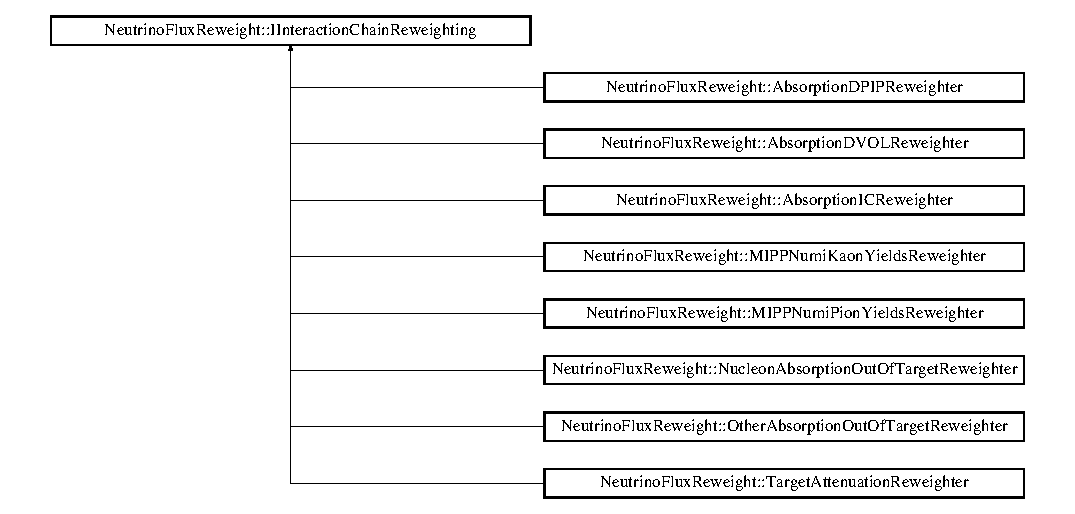
\includegraphics[height=6.461539cm]{class_neutrino_flux_reweight_1_1_i_interaction_chain_reweighting}
\end{center}
\end{figure}
\subsection*{Public Member Functions}
\begin{DoxyCompactItemize}
\item 
virtual \hyperlink{class_neutrino_flux_reweight_1_1_i_interaction_chain_reweighting_a7b521fb6a2f592399446228bd914e94c}{$\sim$\-I\-Interaction\-Chain\-Reweighting} ()
\item 
virtual std\-::vector$<$ bool $>$ \hyperlink{class_neutrino_flux_reweight_1_1_i_interaction_chain_reweighting_aacf17580c1d316f0ebcdfdff7418e9e3}{can\-Reweight} (const \hyperlink{class_neutrino_flux_reweight_1_1_interaction_chain_data}{Interaction\-Chain\-Data} \&)=0
\begin{DoxyCompactList}\small\item\em Look through the \hyperlink{class_neutrino_flux_reweight_1_1_interaction_chain_data}{Interaction\-Chain\-Data} input and identify those Interactions that can be reweighted as part of a chain. We return a vector indicating which elements will be assigned a weight by calculate\-Weight. \end{DoxyCompactList}\item 
virtual double \hyperlink{class_neutrino_flux_reweight_1_1_i_interaction_chain_reweighting_ae28403553637013fdc720674ee24c7c5}{calculate\-Weight} (const \hyperlink{class_neutrino_flux_reweight_1_1_interaction_chain_data}{Interaction\-Chain\-Data} \&)=0
\begin{DoxyCompactList}\small\item\em calculate a weight for this interaction chain given the central value parameters and the parameters for this universe. The weight is something like\-: f(cv)/f(M\-C) $\ast$ f(univ)/f(cv) where cv in this case corresponds to the best value of the parameter, given the data. If univ\-\_\-pars=cv\-\_\-pars then we are calculating a central value weight. Note, \hyperlink{class_neutrino_flux_reweight_1_1_i_interaction_chain_reweighting_aacf17580c1d316f0ebcdfdff7418e9e3}{can\-Reweight()} should be called to determine which elements of the chain are covered by the weight returned by \hyperlink{class_neutrino_flux_reweight_1_1_i_interaction_chain_reweighting_ae28403553637013fdc720674ee24c7c5}{calculate\-Weight()} \end{DoxyCompactList}\end{DoxyCompactItemize}


\subsection{Detailed Description}


Definition at line 17 of file I\-Interaction\-Chain\-Reweighting.\-h.



\subsection{Constructor \& Destructor Documentation}
\hypertarget{class_neutrino_flux_reweight_1_1_i_interaction_chain_reweighting_a7b521fb6a2f592399446228bd914e94c}{\index{Neutrino\-Flux\-Reweight\-::\-I\-Interaction\-Chain\-Reweighting@{Neutrino\-Flux\-Reweight\-::\-I\-Interaction\-Chain\-Reweighting}!$\sim$\-I\-Interaction\-Chain\-Reweighting@{$\sim$\-I\-Interaction\-Chain\-Reweighting}}
\index{$\sim$\-I\-Interaction\-Chain\-Reweighting@{$\sim$\-I\-Interaction\-Chain\-Reweighting}!NeutrinoFluxReweight::IInteractionChainReweighting@{Neutrino\-Flux\-Reweight\-::\-I\-Interaction\-Chain\-Reweighting}}
\subsubsection[{$\sim$\-I\-Interaction\-Chain\-Reweighting}]{\setlength{\rightskip}{0pt plus 5cm}virtual Neutrino\-Flux\-Reweight\-::\-I\-Interaction\-Chain\-Reweighting\-::$\sim$\-I\-Interaction\-Chain\-Reweighting (
\begin{DoxyParamCaption}
{}
\end{DoxyParamCaption}
)\hspace{0.3cm}{\ttfamily [inline]}, {\ttfamily [virtual]}}}\label{class_neutrino_flux_reweight_1_1_i_interaction_chain_reweighting_a7b521fb6a2f592399446228bd914e94c}


Definition at line 20 of file I\-Interaction\-Chain\-Reweighting.\-h.


\begin{DoxyCode}
20 \{\};
\end{DoxyCode}


\subsection{Member Function Documentation}
\hypertarget{class_neutrino_flux_reweight_1_1_i_interaction_chain_reweighting_ae28403553637013fdc720674ee24c7c5}{\index{Neutrino\-Flux\-Reweight\-::\-I\-Interaction\-Chain\-Reweighting@{Neutrino\-Flux\-Reweight\-::\-I\-Interaction\-Chain\-Reweighting}!calculate\-Weight@{calculate\-Weight}}
\index{calculate\-Weight@{calculate\-Weight}!NeutrinoFluxReweight::IInteractionChainReweighting@{Neutrino\-Flux\-Reweight\-::\-I\-Interaction\-Chain\-Reweighting}}
\subsubsection[{calculate\-Weight}]{\setlength{\rightskip}{0pt plus 5cm}virtual double Neutrino\-Flux\-Reweight\-::\-I\-Interaction\-Chain\-Reweighting\-::calculate\-Weight (
\begin{DoxyParamCaption}
\item[{const {\bf Interaction\-Chain\-Data} \&}]{}
\end{DoxyParamCaption}
)\hspace{0.3cm}{\ttfamily [pure virtual]}}}\label{class_neutrino_flux_reweight_1_1_i_interaction_chain_reweighting_ae28403553637013fdc720674ee24c7c5}


calculate a weight for this interaction chain given the central value parameters and the parameters for this universe. The weight is something like\-: f(cv)/f(M\-C) $\ast$ f(univ)/f(cv) where cv in this case corresponds to the best value of the parameter, given the data. If univ\-\_\-pars=cv\-\_\-pars then we are calculating a central value weight. Note, \hyperlink{class_neutrino_flux_reweight_1_1_i_interaction_chain_reweighting_aacf17580c1d316f0ebcdfdff7418e9e3}{can\-Reweight()} should be called to determine which elements of the chain are covered by the weight returned by \hyperlink{class_neutrino_flux_reweight_1_1_i_interaction_chain_reweighting_ae28403553637013fdc720674ee24c7c5}{calculate\-Weight()} 



Implemented in \hyperlink{class_neutrino_flux_reweight_1_1_absorption_d_p_i_p_reweighter_a8b1fcaecb31a3612ec2f5e2a0026bcb6}{Neutrino\-Flux\-Reweight\-::\-Absorption\-D\-P\-I\-P\-Reweighter}, \hyperlink{class_neutrino_flux_reweight_1_1_absorption_d_v_o_l_reweighter_abe4d5b881334283ded041e46d2613608}{Neutrino\-Flux\-Reweight\-::\-Absorption\-D\-V\-O\-L\-Reweighter}, \hyperlink{class_neutrino_flux_reweight_1_1_absorption_i_c_reweighter_a07104ede5adc45dfeda61fc90004bec3}{Neutrino\-Flux\-Reweight\-::\-Absorption\-I\-C\-Reweighter}, \hyperlink{class_neutrino_flux_reweight_1_1_nucleon_absorption_out_of_target_reweighter_a295719b84abffcab3d2cdf3a4aadb7b7}{Neutrino\-Flux\-Reweight\-::\-Nucleon\-Absorption\-Out\-Of\-Target\-Reweighter}, \hyperlink{class_neutrino_flux_reweight_1_1_other_absorption_out_of_target_reweighter_abebfe35083e25e8bca9eb0bf991d74d9}{Neutrino\-Flux\-Reweight\-::\-Other\-Absorption\-Out\-Of\-Target\-Reweighter}, \hyperlink{class_neutrino_flux_reweight_1_1_target_attenuation_reweighter_a58691aeda33f770a28cd27f677ae790f}{Neutrino\-Flux\-Reweight\-::\-Target\-Attenuation\-Reweighter}, \hyperlink{class_neutrino_flux_reweight_1_1_m_i_p_p_numi_kaon_yields_reweighter_ad9503e13848e30f432c297ed70e24134}{Neutrino\-Flux\-Reweight\-::\-M\-I\-P\-P\-Numi\-Kaon\-Yields\-Reweighter}, and \hyperlink{class_neutrino_flux_reweight_1_1_m_i_p_p_numi_pion_yields_reweighter_a84ef113a8ef34c2f9f5813938ec35382}{Neutrino\-Flux\-Reweight\-::\-M\-I\-P\-P\-Numi\-Pion\-Yields\-Reweighter}.

\hypertarget{class_neutrino_flux_reweight_1_1_i_interaction_chain_reweighting_aacf17580c1d316f0ebcdfdff7418e9e3}{\index{Neutrino\-Flux\-Reweight\-::\-I\-Interaction\-Chain\-Reweighting@{Neutrino\-Flux\-Reweight\-::\-I\-Interaction\-Chain\-Reweighting}!can\-Reweight@{can\-Reweight}}
\index{can\-Reweight@{can\-Reweight}!NeutrinoFluxReweight::IInteractionChainReweighting@{Neutrino\-Flux\-Reweight\-::\-I\-Interaction\-Chain\-Reweighting}}
\subsubsection[{can\-Reweight}]{\setlength{\rightskip}{0pt plus 5cm}virtual std\-::vector$<$bool$>$ Neutrino\-Flux\-Reweight\-::\-I\-Interaction\-Chain\-Reweighting\-::can\-Reweight (
\begin{DoxyParamCaption}
\item[{const {\bf Interaction\-Chain\-Data} \&}]{}
\end{DoxyParamCaption}
)\hspace{0.3cm}{\ttfamily [pure virtual]}}}\label{class_neutrino_flux_reweight_1_1_i_interaction_chain_reweighting_aacf17580c1d316f0ebcdfdff7418e9e3}


Look through the \hyperlink{class_neutrino_flux_reweight_1_1_interaction_chain_data}{Interaction\-Chain\-Data} input and identify those Interactions that can be reweighted as part of a chain. We return a vector indicating which elements will be assigned a weight by calculate\-Weight. 



Implemented in \hyperlink{class_neutrino_flux_reweight_1_1_absorption_d_p_i_p_reweighter_a9fc3f50ccda671f623473e43ba49989f}{Neutrino\-Flux\-Reweight\-::\-Absorption\-D\-P\-I\-P\-Reweighter}, \hyperlink{class_neutrino_flux_reweight_1_1_target_attenuation_reweighter_a99789f168f16b45ebf5b02dad6f86cb5}{Neutrino\-Flux\-Reweight\-::\-Target\-Attenuation\-Reweighter}, \hyperlink{class_neutrino_flux_reweight_1_1_absorption_d_v_o_l_reweighter_a4431fee76a4b04a42dac9f6be83f6346}{Neutrino\-Flux\-Reweight\-::\-Absorption\-D\-V\-O\-L\-Reweighter}, \hyperlink{class_neutrino_flux_reweight_1_1_absorption_i_c_reweighter_adb94609e23ec8ee9123abf30d52fae40}{Neutrino\-Flux\-Reweight\-::\-Absorption\-I\-C\-Reweighter}, \hyperlink{class_neutrino_flux_reweight_1_1_nucleon_absorption_out_of_target_reweighter_a978c4e5458a827ff091c990b34515fb7}{Neutrino\-Flux\-Reweight\-::\-Nucleon\-Absorption\-Out\-Of\-Target\-Reweighter}, \hyperlink{class_neutrino_flux_reweight_1_1_other_absorption_out_of_target_reweighter_a5ab6da4e6a66b3ec9bcd24ddb4b90cb1}{Neutrino\-Flux\-Reweight\-::\-Other\-Absorption\-Out\-Of\-Target\-Reweighter}, \hyperlink{class_neutrino_flux_reweight_1_1_m_i_p_p_numi_kaon_yields_reweighter_a6ca3bcd0846fd600f51988a2e396aafb}{Neutrino\-Flux\-Reweight\-::\-M\-I\-P\-P\-Numi\-Kaon\-Yields\-Reweighter}, and \hyperlink{class_neutrino_flux_reweight_1_1_m_i_p_p_numi_pion_yields_reweighter_a6a716b25ddb7d29ace9c7f07d84c91b2}{Neutrino\-Flux\-Reweight\-::\-M\-I\-P\-P\-Numi\-Pion\-Yields\-Reweighter}.



The documentation for this class was generated from the following file\-:\begin{DoxyCompactItemize}
\item 
include/\hyperlink{_i_interaction_chain_reweighting_8h}{I\-Interaction\-Chain\-Reweighting.\-h}\end{DoxyCompactItemize}

\hypertarget{class_neutrino_flux_reweight_1_1_i_interaction_reweighting}{\section{Neutrino\-Flux\-Reweight\-:\-:I\-Interaction\-Reweighting Class Reference}
\label{class_neutrino_flux_reweight_1_1_i_interaction_reweighting}\index{Neutrino\-Flux\-Reweight\-::\-I\-Interaction\-Reweighting@{Neutrino\-Flux\-Reweight\-::\-I\-Interaction\-Reweighting}}
}


{\ttfamily \#include $<$I\-Interaction\-Reweighting.\-h$>$}

Inheritance diagram for Neutrino\-Flux\-Reweight\-:\-:I\-Interaction\-Reweighting\-:\begin{figure}[H]
\begin{center}
\leavevmode
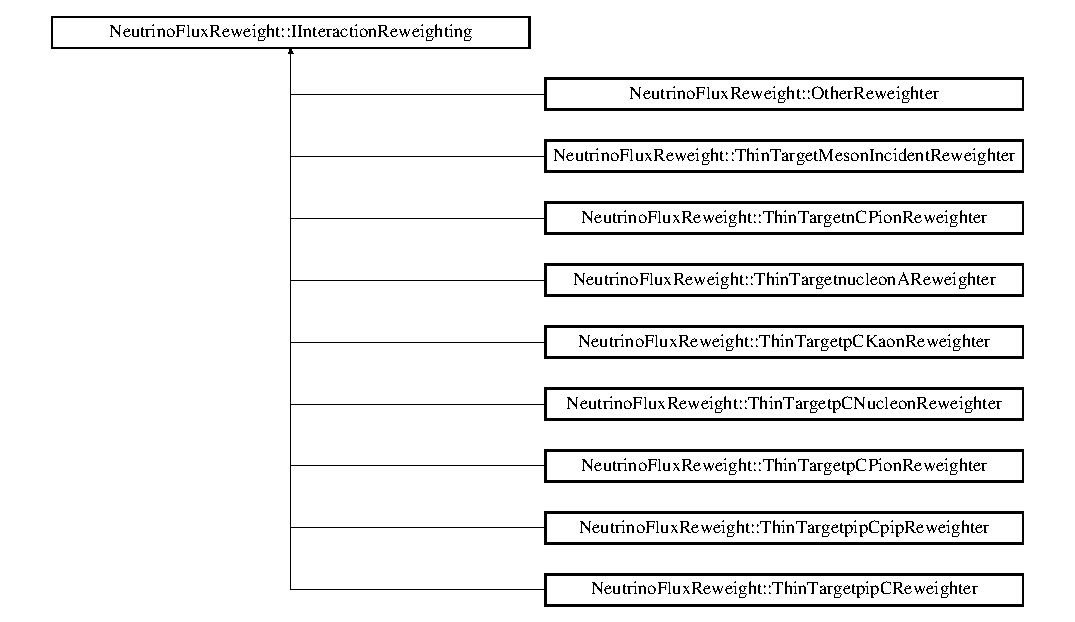
\includegraphics[height=7.909604cm]{class_neutrino_flux_reweight_1_1_i_interaction_reweighting}
\end{center}
\end{figure}
\subsection*{Public Member Functions}
\begin{DoxyCompactItemize}
\item 
virtual \hyperlink{class_neutrino_flux_reweight_1_1_i_interaction_reweighting_a89723625d09e41fa33315dbf4a811d8a}{$\sim$\-I\-Interaction\-Reweighting} ()
\item 
virtual bool \hyperlink{class_neutrino_flux_reweight_1_1_i_interaction_reweighting_aa3d1d3f37a93b02e447cf5eca333ac8d}{can\-Reweight} (const \hyperlink{class_neutrino_flux_reweight_1_1_interaction_data}{Interaction\-Data} \&aa)=0
\begin{DoxyCompactList}\small\item\em can the particular instance of this class reweight this interaction? \end{DoxyCompactList}\item 
virtual double \hyperlink{class_neutrino_flux_reweight_1_1_i_interaction_reweighting_a49b0d73e778411d629205d23575703c3}{calculate\-Weight} (const \hyperlink{class_neutrino_flux_reweight_1_1_interaction_data}{Interaction\-Data} \&inter\-\_\-data)=0
\begin{DoxyCompactList}\small\item\em calculate a weight for this interaction given the central value parameters and the parameters for this universe. The weight is something like\-: f(cv)/f(M\-C) $\ast$ f(univ)/f(cv) where cv in this case corresponds to the best value of the parameter, given the data. If univ\-\_\-pars=cv\-\_\-pars then we are calculating a central value weight \end{DoxyCompactList}\end{DoxyCompactItemize}


\subsection{Detailed Description}


Definition at line 15 of file I\-Interaction\-Reweighting.\-h.



\subsection{Constructor \& Destructor Documentation}
\hypertarget{class_neutrino_flux_reweight_1_1_i_interaction_reweighting_a89723625d09e41fa33315dbf4a811d8a}{\index{Neutrino\-Flux\-Reweight\-::\-I\-Interaction\-Reweighting@{Neutrino\-Flux\-Reweight\-::\-I\-Interaction\-Reweighting}!$\sim$\-I\-Interaction\-Reweighting@{$\sim$\-I\-Interaction\-Reweighting}}
\index{$\sim$\-I\-Interaction\-Reweighting@{$\sim$\-I\-Interaction\-Reweighting}!NeutrinoFluxReweight::IInteractionReweighting@{Neutrino\-Flux\-Reweight\-::\-I\-Interaction\-Reweighting}}
\subsubsection[{$\sim$\-I\-Interaction\-Reweighting}]{\setlength{\rightskip}{0pt plus 5cm}virtual Neutrino\-Flux\-Reweight\-::\-I\-Interaction\-Reweighting\-::$\sim$\-I\-Interaction\-Reweighting (
\begin{DoxyParamCaption}
{}
\end{DoxyParamCaption}
)\hspace{0.3cm}{\ttfamily [inline]}, {\ttfamily [virtual]}}}\label{class_neutrino_flux_reweight_1_1_i_interaction_reweighting_a89723625d09e41fa33315dbf4a811d8a}


Definition at line 17 of file I\-Interaction\-Reweighting.\-h.


\begin{DoxyCode}
17 \{\};
\end{DoxyCode}


\subsection{Member Function Documentation}
\hypertarget{class_neutrino_flux_reweight_1_1_i_interaction_reweighting_a49b0d73e778411d629205d23575703c3}{\index{Neutrino\-Flux\-Reweight\-::\-I\-Interaction\-Reweighting@{Neutrino\-Flux\-Reweight\-::\-I\-Interaction\-Reweighting}!calculate\-Weight@{calculate\-Weight}}
\index{calculate\-Weight@{calculate\-Weight}!NeutrinoFluxReweight::IInteractionReweighting@{Neutrino\-Flux\-Reweight\-::\-I\-Interaction\-Reweighting}}
\subsubsection[{calculate\-Weight}]{\setlength{\rightskip}{0pt plus 5cm}virtual double Neutrino\-Flux\-Reweight\-::\-I\-Interaction\-Reweighting\-::calculate\-Weight (
\begin{DoxyParamCaption}
\item[{const {\bf Interaction\-Data} \&}]{inter\-\_\-data}
\end{DoxyParamCaption}
)\hspace{0.3cm}{\ttfamily [pure virtual]}}}\label{class_neutrino_flux_reweight_1_1_i_interaction_reweighting_a49b0d73e778411d629205d23575703c3}


calculate a weight for this interaction given the central value parameters and the parameters for this universe. The weight is something like\-: f(cv)/f(M\-C) $\ast$ f(univ)/f(cv) where cv in this case corresponds to the best value of the parameter, given the data. If univ\-\_\-pars=cv\-\_\-pars then we are calculating a central value weight 



Implemented in \hyperlink{class_neutrino_flux_reweight_1_1_thin_targetnucleon_a_reweighter_a98d78fabb1cb7fa39372846cb57b0845}{Neutrino\-Flux\-Reweight\-::\-Thin\-Targetnucleon\-A\-Reweighter}, \hyperlink{class_neutrino_flux_reweight_1_1_thin_targetn_c_pion_reweighter_abe918e387700a09d5878cfd22dddfdd8}{Neutrino\-Flux\-Reweight\-::\-Thin\-Targetn\-C\-Pion\-Reweighter}, \hyperlink{class_neutrino_flux_reweight_1_1_other_reweighter_aca4a447053eede66a97747c98a2d89a2}{Neutrino\-Flux\-Reweight\-::\-Other\-Reweighter}, \hyperlink{class_neutrino_flux_reweight_1_1_thin_target_meson_incident_reweighter_adfb3f3e69286e74c6a9c681a0593b4d5}{Neutrino\-Flux\-Reweight\-::\-Thin\-Target\-Meson\-Incident\-Reweighter}, \hyperlink{class_neutrino_flux_reweight_1_1_thin_targetpip_c_reweighter_a6941429f810ddcc72aa979e829da3314}{Neutrino\-Flux\-Reweight\-::\-Thin\-Targetpip\-C\-Reweighter}, \hyperlink{class_neutrino_flux_reweight_1_1_thin_targetp_c_pion_reweighter_ab797bbeeedb04cda73feef891434cd5f}{Neutrino\-Flux\-Reweight\-::\-Thin\-Targetp\-C\-Pion\-Reweighter}, \hyperlink{class_neutrino_flux_reweight_1_1_thin_targetpip_cpip_reweighter_a1491b7320847333a7b6f8b472d4e5ee3}{Neutrino\-Flux\-Reweight\-::\-Thin\-Targetpip\-Cpip\-Reweighter}, \hyperlink{class_neutrino_flux_reweight_1_1_thin_targetp_c_kaon_reweighter_a64f5f6df3b44240b56b863206773ca9a}{Neutrino\-Flux\-Reweight\-::\-Thin\-Targetp\-C\-Kaon\-Reweighter}, and \hyperlink{class_neutrino_flux_reweight_1_1_thin_targetp_c_nucleon_reweighter_a6bf9833d98dab84af820f05cf2ff851b}{Neutrino\-Flux\-Reweight\-::\-Thin\-Targetp\-C\-Nucleon\-Reweighter}.

\hypertarget{class_neutrino_flux_reweight_1_1_i_interaction_reweighting_aa3d1d3f37a93b02e447cf5eca333ac8d}{\index{Neutrino\-Flux\-Reweight\-::\-I\-Interaction\-Reweighting@{Neutrino\-Flux\-Reweight\-::\-I\-Interaction\-Reweighting}!can\-Reweight@{can\-Reweight}}
\index{can\-Reweight@{can\-Reweight}!NeutrinoFluxReweight::IInteractionReweighting@{Neutrino\-Flux\-Reweight\-::\-I\-Interaction\-Reweighting}}
\subsubsection[{can\-Reweight}]{\setlength{\rightskip}{0pt plus 5cm}virtual bool Neutrino\-Flux\-Reweight\-::\-I\-Interaction\-Reweighting\-::can\-Reweight (
\begin{DoxyParamCaption}
\item[{const {\bf Interaction\-Data} \&}]{aa}
\end{DoxyParamCaption}
)\hspace{0.3cm}{\ttfamily [pure virtual]}}}\label{class_neutrino_flux_reweight_1_1_i_interaction_reweighting_aa3d1d3f37a93b02e447cf5eca333ac8d}


can the particular instance of this class reweight this interaction? 



Implemented in \hyperlink{class_neutrino_flux_reweight_1_1_thin_targetnucleon_a_reweighter_ac412a741a29973bbefbb3daa0cf6636a}{Neutrino\-Flux\-Reweight\-::\-Thin\-Targetnucleon\-A\-Reweighter}, \hyperlink{class_neutrino_flux_reweight_1_1_thin_targetn_c_pion_reweighter_aaeb028c4bd75fcbbae6e03aba3a7e85a}{Neutrino\-Flux\-Reweight\-::\-Thin\-Targetn\-C\-Pion\-Reweighter}, \hyperlink{class_neutrino_flux_reweight_1_1_other_reweighter_af5cadc4dcde8b9884962399b0a29bc5a}{Neutrino\-Flux\-Reweight\-::\-Other\-Reweighter}, \hyperlink{class_neutrino_flux_reweight_1_1_thin_target_meson_incident_reweighter_ad6974a8bf1b26e86252ee2bc1e112c5a}{Neutrino\-Flux\-Reweight\-::\-Thin\-Target\-Meson\-Incident\-Reweighter}, \hyperlink{class_neutrino_flux_reweight_1_1_thin_targetpip_c_reweighter_a85dfb364850ec5af9b58cdff4c37c678}{Neutrino\-Flux\-Reweight\-::\-Thin\-Targetpip\-C\-Reweighter}, \hyperlink{class_neutrino_flux_reweight_1_1_thin_targetp_c_pion_reweighter_a09067dcacb294ca133e2660d61302e85}{Neutrino\-Flux\-Reweight\-::\-Thin\-Targetp\-C\-Pion\-Reweighter}, \hyperlink{class_neutrino_flux_reweight_1_1_thin_targetpip_cpip_reweighter_a0a7a18f342e8c88715671e3804dbd1ca}{Neutrino\-Flux\-Reweight\-::\-Thin\-Targetpip\-Cpip\-Reweighter}, \hyperlink{class_neutrino_flux_reweight_1_1_thin_targetp_c_kaon_reweighter_a78d9307c378b36d660feb54ba8114a9a}{Neutrino\-Flux\-Reweight\-::\-Thin\-Targetp\-C\-Kaon\-Reweighter}, and \hyperlink{class_neutrino_flux_reweight_1_1_thin_targetp_c_nucleon_reweighter_a974bafd329ce322beef237061f446694}{Neutrino\-Flux\-Reweight\-::\-Thin\-Targetp\-C\-Nucleon\-Reweighter}.



The documentation for this class was generated from the following file\-:\begin{DoxyCompactItemize}
\item 
include/\hyperlink{_i_interaction_reweighting_8h}{I\-Interaction\-Reweighting.\-h}\end{DoxyCompactItemize}

\hypertarget{class_neutrino_flux_reweight_1_1_interaction_chain_data}{\section{Neutrino\-Flux\-Reweight\-:\-:Interaction\-Chain\-Data Class Reference}
\label{class_neutrino_flux_reweight_1_1_interaction_chain_data}\index{Neutrino\-Flux\-Reweight\-::\-Interaction\-Chain\-Data@{Neutrino\-Flux\-Reweight\-::\-Interaction\-Chain\-Data}}
}


Information about the chain of interactions leading to a neutrino.  




{\ttfamily \#include $<$Interaction\-Chain\-Data.\-h$>$}

\subsection*{Public Member Functions}
\begin{DoxyCompactItemize}
\item 
\hyperlink{class_neutrino_flux_reweight_1_1_interaction_chain_data_aa936bc29461049e00fe62ccf528db2eb}{Interaction\-Chain\-Data} ()
\begin{DoxyCompactList}\small\item\em boring old default constructor \end{DoxyCompactList}\item 
\hyperlink{class_neutrino_flux_reweight_1_1_interaction_chain_data_af2ab1388c8d0c81c53b31f9c3e22fb4e}{Interaction\-Chain\-Data} (\hyperlink{classnu__g4numi}{nu\-\_\-g4numi} $\ast$nu, const char $\ast$tgtcfg, const char $\ast$horncfg)
\item 
\hyperlink{class_neutrino_flux_reweight_1_1_interaction_chain_data_ae8ee384bee786269c30073a2a9600d31}{Interaction\-Chain\-Data} (bsim\-::\-Dk2\-Nu $\ast$nu, bsim\-::\-Dk\-Meta $\ast$meta)
\begin{DoxyCompactList}\small\item\em create an interaction chain from the new dk2nu format \end{DoxyCompactList}\item 
std\-::ostream \& \hyperlink{class_neutrino_flux_reweight_1_1_interaction_chain_data_a27b0c5dc28fcec9536ed6dddf79d0501}{print} (std\-::ostream \&os=std\-::cout) const 
\end{DoxyCompactItemize}
\subsection*{Public Attributes}
\begin{DoxyCompactItemize}
\item 
std\-::vector$<$ \hyperlink{class_neutrino_flux_reweight_1_1_interaction_data}{Interaction\-Data} $>$ \hyperlink{class_neutrino_flux_reweight_1_1_interaction_chain_data_a5864063b9c20b4f70e4f1e355df21963}{interaction\-\_\-chain}
\begin{DoxyCompactList}\small\item\em vector of neutrino ancestors \end{DoxyCompactList}\item 
\hyperlink{class_neutrino_flux_reweight_1_1_target_data}{Target\-Data} \hyperlink{class_neutrino_flux_reweight_1_1_interaction_chain_data_a6df89bff97001a4988487fcfb9f4acea}{tar\-\_\-info}
\begin{DoxyCompactList}\small\item\em Information about the hadron which exited the target. \end{DoxyCompactList}\item 
std\-::vector\\*
$<$ \hyperlink{class_neutrino_flux_reweight_1_1_particles_through_volumes_data}{Particles\-Through\-Volumes\-Data} $>$ \hyperlink{class_neutrino_flux_reweight_1_1_interaction_chain_data_adda6bc8863579964b62e3d4f51e14926}{ptv\-\_\-info}
\begin{DoxyCompactList}\small\item\em Information about all particles that pass through volumes without interacting. \end{DoxyCompactList}\item 
std\-::string \hyperlink{class_neutrino_flux_reweight_1_1_interaction_chain_data_a8362a0f94df2bd321e0b60a38c41fb7a}{target\-\_\-config}
\begin{DoxyCompactList}\small\item\em The target configuration. Example\-: le010z. \end{DoxyCompactList}\item 
std\-::string \hyperlink{class_neutrino_flux_reweight_1_1_interaction_chain_data_a343d6a28ec2d41252a6067833b75f831}{horn\-\_\-config}
\begin{DoxyCompactList}\small\item\em The horn configuration. Example\-: 185i. \end{DoxyCompactList}\item 
int \hyperlink{class_neutrino_flux_reweight_1_1_interaction_chain_data_aca185ce4c11a46ea16b29a55ff97a490}{playlist}
\begin{DoxyCompactList}\small\item\em The tgt playlist (exact position of the target after survey) \end{DoxyCompactList}\end{DoxyCompactItemize}
\subsection*{Private Member Functions}
\begin{DoxyCompactItemize}
\item 
bool \hyperlink{class_neutrino_flux_reweight_1_1_interaction_chain_data_a4297c9ba702c5c205e9624b8bdcc6471}{is\-\_\-fast\-\_\-decay} (int pdg)
\end{DoxyCompactItemize}


\subsection{Detailed Description}
Information about the chain of interactions leading to a neutrino. 

Definition at line 19 of file Interaction\-Chain\-Data.\-h.



\subsection{Constructor \& Destructor Documentation}
\hypertarget{class_neutrino_flux_reweight_1_1_interaction_chain_data_aa936bc29461049e00fe62ccf528db2eb}{\index{Neutrino\-Flux\-Reweight\-::\-Interaction\-Chain\-Data@{Neutrino\-Flux\-Reweight\-::\-Interaction\-Chain\-Data}!Interaction\-Chain\-Data@{Interaction\-Chain\-Data}}
\index{Interaction\-Chain\-Data@{Interaction\-Chain\-Data}!NeutrinoFluxReweight::InteractionChainData@{Neutrino\-Flux\-Reweight\-::\-Interaction\-Chain\-Data}}
\subsubsection[{Interaction\-Chain\-Data}]{\setlength{\rightskip}{0pt plus 5cm}Neutrino\-Flux\-Reweight\-::\-Interaction\-Chain\-Data\-::\-Interaction\-Chain\-Data (
\begin{DoxyParamCaption}
{}
\end{DoxyParamCaption}
)}}\label{class_neutrino_flux_reweight_1_1_interaction_chain_data_aa936bc29461049e00fe62ccf528db2eb}


boring old default constructor 



Definition at line 6 of file Interaction\-Chain\-Data.\-cpp.


\begin{DoxyCode}
6 \{\}
\end{DoxyCode}
\hypertarget{class_neutrino_flux_reweight_1_1_interaction_chain_data_af2ab1388c8d0c81c53b31f9c3e22fb4e}{\index{Neutrino\-Flux\-Reweight\-::\-Interaction\-Chain\-Data@{Neutrino\-Flux\-Reweight\-::\-Interaction\-Chain\-Data}!Interaction\-Chain\-Data@{Interaction\-Chain\-Data}}
\index{Interaction\-Chain\-Data@{Interaction\-Chain\-Data}!NeutrinoFluxReweight::InteractionChainData@{Neutrino\-Flux\-Reweight\-::\-Interaction\-Chain\-Data}}
\subsubsection[{Interaction\-Chain\-Data}]{\setlength{\rightskip}{0pt plus 5cm}Neutrino\-Flux\-Reweight\-::\-Interaction\-Chain\-Data\-::\-Interaction\-Chain\-Data (
\begin{DoxyParamCaption}
\item[{{\bf nu\-\_\-g4numi} $\ast$}]{nu, }
\item[{const char $\ast$}]{tgtcfg, }
\item[{const char $\ast$}]{horncfg}
\end{DoxyParamCaption}
)}}\label{class_neutrino_flux_reweight_1_1_interaction_chain_data_af2ab1388c8d0c81c53b31f9c3e22fb4e}
create an interaction chain from the old g4numi nudata structure tgtcfg specified the target configuration. Example\-: le010z horncfg specifies the horn configuration. Example\-: 185i 

Definition at line 7 of file Interaction\-Chain\-Data.\-cpp.


\begin{DoxyCode}
9                                                                  \{
10     
11     \textcolor{comment}{// Fill in information about the hadron exiting the target}
12     \textcolor{comment}{// this information is needed in order to reweight yields}
13     \textcolor{comment}{// off the target (i.e., MIPP)}
14     \textcolor{keywordtype}{double} tarP[3];
15     tarP[0] = nu->\hyperlink{classnu__g4numi_a8693b10daf61759ad2decb2c3aac6a9e}{tpx};
16     tarP[1] = nu->\hyperlink{classnu__g4numi_a533f9a7e3002a702856c25dd1e5c7058}{tpy};
17     tarP[2] = nu->\hyperlink{classnu__g4numi_a63eb35fe1697f426543e34652202e30b}{tpz};
18     \textcolor{keywordtype}{double} tarV[3];
19     tarV[0] = nu->\hyperlink{classnu__g4numi_a8675345bdaaec6f0d4ff5f57571133a0}{tvx};
20     tarV[1] = nu->\hyperlink{classnu__g4numi_ac81b906ee11d4c5e74a1b80378cae373}{tvy};
21     tarV[2] = nu->\hyperlink{classnu__g4numi_adef9f7bf0e713b329e9af89ae32183ab}{tvz};
22     
23     \textcolor{keyword}{static} \hyperlink{class_numi2_pdg}{Numi2Pdg} numi2pdg;
24     \hyperlink{class_neutrino_flux_reweight_1_1_interaction_chain_data_a6df89bff97001a4988487fcfb9f4acea}{tar\_info} = TargetData(tarP,numi2pdg.\hyperlink{class_numi2_pdg_ac8d5438ffd52928a82738feed56e4f90}{GetPdg}(nu->\hyperlink{classnu__g4numi_a1047ac371479cee32c28f56adf885515}{tptype}),tarV,-1);
25     
26     \textcolor{comment}{// loop over trajectories, create InteractionData objects,}
27     \textcolor{comment}{// and add them to the interaction\_chain vector    }
28     \textcolor{comment}{//(Note about units: In nudata format, the momentum unit is MeV)}
29     
30     Int\_t ntraj = nu->\hyperlink{classnu__g4numi_abdbe76af4b20f3b5b5b2fb4b92156b42}{ntrajectory};
31     \textcolor{keywordflow}{if}(ntraj>10)ntraj = 10;
32     \textcolor{keywordflow}{for}(\textcolor{keywordtype}{int} itraj=0;itraj<(ntraj-1);itraj++)\{
33       \textcolor{keywordtype}{double} incP[3];
34       incP[0] = nu->\hyperlink{classnu__g4numi_a11ce125811f5f35337733e18f3753d31}{pprodpx}[itraj+1]/1000.;
35       incP[1] = nu->\hyperlink{classnu__g4numi_a7fa5412e9c5006b884f09226ae2c350a}{pprodpy}[itraj+1]/1000.;
36       incP[2] = nu->\hyperlink{classnu__g4numi_a0bd7772ccdfe00660ce45d94c107a240}{pprodpz}[itraj+1]/1000.;
37       
38       Int\_t itraj\_prod = itraj + 1;
39       Int\_t pdg\_prod   = nu->\hyperlink{classnu__g4numi_a4ed6688aee6debd26637a0401e5ef475}{pdg}[itraj\_prod];
40       std::string this\_proc = std::string(nu->\hyperlink{classnu__g4numi_a6583de2ce34a5d19409c09cc0b63692f}{proc}[itraj\_prod]);
41       \textcolor{comment}{// skip over etas and other swiftly decaying particles}
42       \textcolor{comment}{// we are interested in their daughters}
43  
44       \textcolor{comment}{//It seems that the next while is causing seg fault in gcc 6.3:}
45       \textcolor{comment}{/*  while( is\_fast\_decay(pdg\_prod) )\{}
46 \textcolor{comment}{          itraj\_prod++;}
47 \textcolor{comment}{          pdg\_prod = nu->pdg[itraj\_prod];}
48 \textcolor{comment}{          \} */}   
49       \textcolor{keywordflow}{if}( \hyperlink{class_neutrino_flux_reweight_1_1_interaction_chain_data_a4297c9ba702c5c205e9624b8bdcc6471}{is\_fast\_decay}(pdg\_prod) )\{
50         \textcolor{keywordflow}{for}(\textcolor{keywordtype}{int} ifast = itraj\_prod + 1; ifast < (ntraj-1); ifast++ )\{
51           pdg\_prod = nu->\hyperlink{classnu__g4numi_a4ed6688aee6debd26637a0401e5ef475}{pdg}[ifast];
52           itraj\_prod++;
53           pdg\_prod = nu->\hyperlink{classnu__g4numi_a4ed6688aee6debd26637a0401e5ef475}{pdg}[itraj\_prod];
54           \textcolor{keywordflow}{if}( !\hyperlink{class_neutrino_flux_reweight_1_1_interaction_chain_data_a4297c9ba702c5c205e9624b8bdcc6471}{is\_fast\_decay}(pdg\_prod) ) \textcolor{keywordflow}{break};      
55         \}
56       \}        
57       \textcolor{keywordtype}{double} prodP[3];
58       prodP[0] = nu->\hyperlink{classnu__g4numi_a309ea4b88683c5978593c0d474b1a976}{startpx}[itraj\_prod]/1000.;
59       prodP[1] = nu->\hyperlink{classnu__g4numi_a5247e8e73a100a7064f032806f542d38}{startpy}[itraj\_prod]/1000.;
60       prodP[2] = nu->\hyperlink{classnu__g4numi_a6bec79e4a2effa3cdaa28a1f02ae8124}{startpz}[itraj\_prod]/1000.;
61       
62       \textcolor{keywordtype}{double} vtx[3];
63       vtx[0]=nu->\hyperlink{classnu__g4numi_ab9ea407b9c38c0c73b606d9f6f4df80a}{startx}[itraj\_prod];
64       vtx[1]=nu->\hyperlink{classnu__g4numi_a58d39dbb466f353155aca6a6e7a2cc12}{starty}[itraj\_prod];
65       vtx[2]=nu->\hyperlink{classnu__g4numi_afc1991c5be450f31577f4e1d31dceb2f}{startz}[itraj\_prod];
66 
67       InteractionData inter(itraj, incP,nu->\hyperlink{classnu__g4numi_a4ed6688aee6debd26637a0401e5ef475}{pdg}[itraj],prodP,pdg\_prod,std::string(nu->
      \hyperlink{classnu__g4numi_a72d170869c1eb191d10366d07024417c}{fvol}[itraj]),this\_proc,vtx);   
68       \hyperlink{class_neutrino_flux_reweight_1_1_interaction_chain_data_a5864063b9c20b4f70e4f1e355df21963}{interaction\_chain}.push\_back(inter);
69     \}
70     
71     \textcolor{comment}{//}
72     \textcolor{comment}{//nothing to fill for ParticlesThroughVolumesData here. If we are using nudata format}
73     \textcolor{comment}{//the size of the vector of ParticlesThroughVolumesData objects will be zero.}
74     \textcolor{comment}{//    }
75 
76     \hyperlink{class_neutrino_flux_reweight_1_1_interaction_chain_data_a8362a0f94df2bd321e0b60a38c41fb7a}{target\_config}=tgtcfg;
77     \hyperlink{class_neutrino_flux_reweight_1_1_interaction_chain_data_a343d6a28ec2d41252a6067833b75f831}{horn\_config}=horncfg;
78     \hyperlink{class_neutrino_flux_reweight_1_1_interaction_chain_data_aca185ce4c11a46ea16b29a55ff97a490}{playlist} = -1;
79   \}
\end{DoxyCode}
\hypertarget{class_neutrino_flux_reweight_1_1_interaction_chain_data_ae8ee384bee786269c30073a2a9600d31}{\index{Neutrino\-Flux\-Reweight\-::\-Interaction\-Chain\-Data@{Neutrino\-Flux\-Reweight\-::\-Interaction\-Chain\-Data}!Interaction\-Chain\-Data@{Interaction\-Chain\-Data}}
\index{Interaction\-Chain\-Data@{Interaction\-Chain\-Data}!NeutrinoFluxReweight::InteractionChainData@{Neutrino\-Flux\-Reweight\-::\-Interaction\-Chain\-Data}}
\subsubsection[{Interaction\-Chain\-Data}]{\setlength{\rightskip}{0pt plus 5cm}Neutrino\-Flux\-Reweight\-::\-Interaction\-Chain\-Data\-::\-Interaction\-Chain\-Data (
\begin{DoxyParamCaption}
\item[{bsim\-::\-Dk2\-Nu $\ast$}]{nu, }
\item[{bsim\-::\-Dk\-Meta $\ast$}]{meta}
\end{DoxyParamCaption}
)}}\label{class_neutrino_flux_reweight_1_1_interaction_chain_data_ae8ee384bee786269c30073a2a9600d31}


create an interaction chain from the new dk2nu format 



Definition at line 81 of file Interaction\-Chain\-Data.\-cpp.


\begin{DoxyCode}
82                                                               \{
83     
84     \textcolor{comment}{// Fill in information about the hadron exiting the target}
85     \textcolor{comment}{// this information is needed in order to reweight yields}
86     \textcolor{comment}{// off the target (i.e., MIPP)}
87     std::string mode(getenv(\textcolor{stringliteral}{"MODE"}));
88     \textcolor{comment}{//if(mode=="OPT")std::cout<<"MODE IS OPT interactionchaindata "<<std::endl;}
89     \textcolor{comment}{//else std::cout<<"MODE not recognized. InteractionChainData "<<std::endl;}
90     
91    \textcolor{comment}{// std::cout<<" The environment is "<<getenv("MODE")<<std::endl;}
92     \textcolor{keywordtype}{double} tarP[3];
93     tarP[0]=nu->tgtexit.tpx;
94     tarP[1]=nu->tgtexit.tpy;
95     tarP[2]=nu->tgtexit.tpz;
96     \textcolor{keywordtype}{double} tarV[3];
97     tarV[0]=nu->tgtexit.tvx;
98     tarV[1]=nu->tgtexit.tvy;
99     tarV[2]=nu->tgtexit.tvz;
100     \textcolor{keywordtype}{int} Nskip = 0;
101     \textcolor{comment}{//we will fill tardata after looking into the ancestry for the right index.}
102     
103     \textcolor{comment}{// loop over trajectories, create InteractionData objects,}
104     \textcolor{comment}{// and add them to the interaction\_chain vector}
105     \textcolor{comment}{// Note about units: In dk2nu format, the momentum unit is GeV}
106 
107     Int\_t ntraj = nu->ancestor.size();
108     \textcolor{keywordflow}{for}(\textcolor{keywordtype}{int} itraj=0;itraj<(ntraj-1);itraj++)\{
109       
110       \textcolor{keywordtype}{int} pdg\_inc=nu->ancestor[itraj].pdg;
111       \textcolor{keywordtype}{double} incP[3];
112       incP[0]=0.0;incP[1]=0.0;incP[2]=0.0;
113       \textcolor{comment}{// itraj is the index of the projectile in each interaction.}
114       \textcolor{comment}{// one can find out what it did by looking at}
115       \textcolor{comment}{//       ancestor[itraj+1].proc}
116       \textcolor{comment}{// since 'proc' records the process which made the particle.}
117       \textcolor{comment}{//}
118       \textcolor{comment}{// Unfortunately, the pprod variables in g4numi v5 are needlessly complicated}
119       \textcolor{comment}{//}
120       \textcolor{comment}{// (1) If the particle at itraj *interacts* then pprod seems to hold}
121       \textcolor{comment}{// the momentum of the particle just before the interaction}
122       \textcolor{comment}{// }
123       \textcolor{comment}{// (2) If the particle at itraj *decays* then pprod seems to hold the}
124       \textcolor{comment}{// momentum of the particle at itraj-1, just before it interacts}
125       \textcolor{comment}{//}
126       \textcolor{comment}{// (3) If the particle at itraj is the *result of a decay*, then pprod holds}
127       \textcolor{comment}{// something that looks like the momentum of the parent.}
128       \textcolor{comment}{//}
129       \textcolor{comment}{// Generally for hadron production studies, the second case isn't interesting}
130     \textcolor{comment}{//  if(nu->ancestor[itraj].pprodpz==0)std::cout<<"Found incident proton with 0 GeV Energy"<<std::endl;}
131       \textcolor{keywordflow}{if}( nu->ancestor[itraj].pprodpz != 0)\{
132         incP[0] = nu->ancestor[itraj].pprodpx;
133         incP[1] = nu->ancestor[itraj].pprodpy;
134         incP[2] = nu->ancestor[itraj].pprodpz;
135       
136       \}
137       \textcolor{keywordflow}{else}\{
138         incP[0]=nu->ancestor[itraj].stoppx;
139         incP[1]=nu->ancestor[itraj].stoppy;
140         incP[2]=nu->ancestor[itraj].stoppz;
141       \}
142       Int\_t itraj\_prod = itraj + 1;
143       Int\_t pdg\_prod   = nu->ancestor[itraj\_prod].pdg;
144       std::string this\_proc = std::string(nu->ancestor[itraj\_prod].proc);
145       
146       \textcolor{comment}{// skip over etas and other swiftly decaying particles}
147       \textcolor{comment}{// we are interested in their daughters}
148       \textcolor{comment}{//It seems that the next while is causing seg fault in gcc 6.3:}
149       \textcolor{comment}{/*while( is\_fast\_decay(pdg\_prod) )\{}
150 \textcolor{comment}{        itraj\_prod++;}
151 \textcolor{comment}{        Nskip++;}
152 \textcolor{comment}{        pdg\_prod = nu->ancestor[itraj\_prod].pdg;}
153 \textcolor{comment}{        \}*/}
154       \textcolor{keywordflow}{if}( \hyperlink{class_neutrino_flux_reweight_1_1_interaction_chain_data_a4297c9ba702c5c205e9624b8bdcc6471}{is\_fast\_decay}(pdg\_prod) )\{
155         \textcolor{keywordflow}{for}(\textcolor{keywordtype}{int} ifast = itraj\_prod + 1; ifast < (ntraj-1); ifast++ )\{
156           itraj\_prod++;
157           Nskip++;
158           pdg\_prod = nu->ancestor[itraj\_prod].pdg;
159           \textcolor{keywordflow}{if}( !\hyperlink{class_neutrino_flux_reweight_1_1_interaction_chain_data_a4297c9ba702c5c205e9624b8bdcc6471}{is\_fast\_decay}(pdg\_prod) ) \textcolor{keywordflow}{break};      
160         \}
161       \}
162       \textcolor{keywordtype}{double} prodP[3];
163       prodP[0] = nu->ancestor[itraj\_prod].startpx;
164       prodP[1] = nu->ancestor[itraj\_prod].startpy;
165       prodP[2] = nu->ancestor[itraj\_prod].startpz;
166       
167       \textcolor{keywordtype}{double} vtx[3];
168       vtx[0]=nu->ancestor[itraj\_prod].startx;
169       vtx[1]=nu->ancestor[itraj\_prod].starty;
170       vtx[2]=nu->ancestor[itraj\_prod].startz;
171       std::string this\_vol=nu->ancestor[itraj\_prod].ivol;
172       
173       \textcolor{comment}{//Get Rid of Hydrogen}
174         \textcolor{keywordflow}{if}(pdg\_prod == 1000010020 || pdg\_inc == 1000010020|| pdg\_inc == 1000020030||pdg\_prod==1000020030)\{
175       \textcolor{comment}{// std::cout<<"InteractionChainData::Unusual pdgcode found "<<pdg\_prod<<std::endl; //For now just
       skipping these deuterons}
176         \textcolor{keywordflow}{continue};
177         \}
178       
179       InteractionData inter(itraj, incP,pdg\_inc,prodP,pdg\_prod,
180                             this\_vol,this\_proc,vtx);   
181       \hyperlink{class_neutrino_flux_reweight_1_1_interaction_chain_data_a5864063b9c20b4f70e4f1e355df21963}{interaction\_chain}.push\_back(inter);
182 
183     \}\textcolor{comment}{// end loop over trajectories}
184     \textcolor{comment}{/*&int tptype = numi2pdg.GetPdg(nu->tgtexit.tptype);}
185 \textcolor{comment}{    if(mode=="NUMI")tptype = nu->tgtexit.tptype; this was added by DUNE... seems not right (Leo) */}
186       \textcolor{comment}{//  std::cout<<"The tptype::InteractionChainData "<<tptype<<" "<<nu->tgtexit.tptype<<std::endl;}
187     \textcolor{keywordflow}{if}(meta->vintnames.size()==0)\{
188       \hyperlink{class_neutrino_flux_reweight_1_1_interaction_chain_data_a6df89bff97001a4988487fcfb9f4acea}{tar\_info} = TargetData(tarP,nu->tgtexit.tptype,tarV,-1);
189     \}
190     \textcolor{keywordflow}{else}\{    
191       \hyperlink{class_neutrino_flux_reweight_1_1_interaction_chain_data_a6df89bff97001a4988487fcfb9f4acea}{tar\_info} = TargetData(tarP,nu->tgtexit.tptype,tarV,nu->vint[0]-Nskip);
192     \}
193     
194     \textcolor{comment}{//Filling here the ParticlesThroughVolumesData info:}
195     \hyperlink{class_neutrino_flux_reweight_1_1_interaction_chain_data_adda6bc8863579964b62e3d4f51e14926}{ptv\_info}.clear();
196     \textcolor{comment}{//Looking IC, DPIP and DVOL:}
197     \textcolor{keywordtype}{int} pdgs[3];
198     \textcolor{keywordtype}{double} moms[3];
199     \textcolor{keywordtype}{double} amount\_IC[3],amount\_DPIP[3],amount\_DVOL[3];
200     \textcolor{keywordflow}{for}(\textcolor{keywordtype}{int} ii=0;ii<3;ii++)\{
201       pdgs[ii] = 0; moms[ii] = 0; 
202       amount\_IC[ii] = 0; amount\_DPIP[ii] = 0; amount\_DVOL[ii] = 0;
203     \}
204     
205     \textcolor{keywordflow}{for}(\textcolor{keywordtype}{int} ii=0;ii<3;ii++)\{
206       \textcolor{keywordflow}{if}(nu->ancestor.size()==3 && ii==2)\textcolor{keywordflow}{continue};
207       pdgs[ii] = nu->ancestor[nu->ancestor.size()-ii-2].pdg;
208       moms[ii] = sqrt(pow(nu->ancestor[nu->ancestor.size()-ii-2].startpx,2)+
209                         pow(nu->ancestor[nu->ancestor.size()-ii-2].startpy,2)+
210                         pow(nu->ancestor[nu->ancestor.size()-ii-2].startpz,2));
211       
212       \textcolor{comment}{//Amounts:}
213       \textcolor{comment}{//control:}
214       \textcolor{keywordflow}{if}( (nu->vdbl)[ii] <0 || (nu->vdbl)[ii+3] <0 || (nu->vdbl)[ii+6] <0 || (nu->vdbl)[ii+9] <0)\{
215         std::cout<< \textcolor{stringliteral}{"ERROR FILLING AMOUNT OF MATERIAL CROSSED (In InteractionChainData) !!!"} <<std::endl;
216       \}
217       amount\_IC[ii]   = (nu->vdbl)[ii] + (nu->vdbl)[ii+3];
218       amount\_DPIP[ii] = (nu->vdbl)[ii+6];
219       amount\_DVOL[ii] = (nu->vdbl)[ii+9];
220     \}
221     
222     ParticlesThroughVolumesData tmp\_ptv\_IC(pdgs,amount\_IC,moms,\textcolor{stringliteral}{"IC"});
223     ParticlesThroughVolumesData tmp\_ptv\_DPIP(pdgs,amount\_DPIP,moms,\textcolor{stringliteral}{"DPIP"});
224     ParticlesThroughVolumesData tmp\_ptv\_DVOL(pdgs,amount\_DVOL,moms,\textcolor{stringliteral}{"DVOL"});
225     
226     \hyperlink{class_neutrino_flux_reweight_1_1_interaction_chain_data_adda6bc8863579964b62e3d4f51e14926}{ptv\_info}.push\_back(tmp\_ptv\_IC);
227     \hyperlink{class_neutrino_flux_reweight_1_1_interaction_chain_data_adda6bc8863579964b62e3d4f51e14926}{ptv\_info}.push\_back(tmp\_ptv\_DPIP);
228     \hyperlink{class_neutrino_flux_reweight_1_1_interaction_chain_data_adda6bc8863579964b62e3d4f51e14926}{ptv\_info}.push\_back(tmp\_ptv\_DVOL);\textcolor{comment}{}
229 \textcolor{comment}{    ///}
230 \textcolor{comment}{}    
231     \hyperlink{class_neutrino_flux_reweight_1_1_interaction_chain_data_a8362a0f94df2bd321e0b60a38c41fb7a}{target\_config}=meta->tgtcfg;
232     \hyperlink{class_neutrino_flux_reweight_1_1_interaction_chain_data_a343d6a28ec2d41252a6067833b75f831}{horn\_config}=meta->horncfg;
233     \textcolor{keywordflow}{if}((mode==\textcolor{stringliteral}{"REF"})||(mode==\textcolor{stringliteral}{"OPT"}))\hyperlink{class_neutrino_flux_reweight_1_1_interaction_chain_data_a8362a0f94df2bd321e0b60a38c41fb7a}{target\_config} = \textcolor{stringliteral}{"le00zmi"};
234     \textcolor{comment}{//special tgt configuration for Minerva (exact longitudinal position after survey)}
235     \textcolor{comment}{//check for other experiments}
236     \textcolor{keywordflow}{if}(meta->vintnames.size()>1)\{
237       \hyperlink{class_neutrino_flux_reweight_1_1_interaction_chain_data_aca185ce4c11a46ea16b29a55ff97a490}{playlist} = nu->vint[1];
238     \}
239     \textcolor{keywordflow}{else}\{
240       \hyperlink{class_neutrino_flux_reweight_1_1_interaction_chain_data_aca185ce4c11a46ea16b29a55ff97a490}{playlist} = -1;
241     \}
242     
243   \}
\end{DoxyCode}


\subsection{Member Function Documentation}
\hypertarget{class_neutrino_flux_reweight_1_1_interaction_chain_data_a4297c9ba702c5c205e9624b8bdcc6471}{\index{Neutrino\-Flux\-Reweight\-::\-Interaction\-Chain\-Data@{Neutrino\-Flux\-Reweight\-::\-Interaction\-Chain\-Data}!is\-\_\-fast\-\_\-decay@{is\-\_\-fast\-\_\-decay}}
\index{is\-\_\-fast\-\_\-decay@{is\-\_\-fast\-\_\-decay}!NeutrinoFluxReweight::InteractionChainData@{Neutrino\-Flux\-Reweight\-::\-Interaction\-Chain\-Data}}
\subsubsection[{is\-\_\-fast\-\_\-decay}]{\setlength{\rightskip}{0pt plus 5cm}bool Neutrino\-Flux\-Reweight\-::\-Interaction\-Chain\-Data\-::is\-\_\-fast\-\_\-decay (
\begin{DoxyParamCaption}
\item[{int}]{pdg}
\end{DoxyParamCaption}
)\hspace{0.3cm}{\ttfamily [private]}}}\label{class_neutrino_flux_reweight_1_1_interaction_chain_data_a4297c9ba702c5c205e9624b8bdcc6471}


Definition at line 265 of file Interaction\-Chain\-Data.\-cpp.


\begin{DoxyCode}
265                                                  \{
266     
267     \textcolor{keywordtype}{bool} fast\_decay = \textcolor{keyword}{false};
268     \textcolor{keywordflow}{if}( (pdg==221)||(pdg==331)||(pdg==3212)||(pdg==113)||(pdg==223) )fast\_decay = \textcolor{keyword}{true};
269     \textcolor{keywordflow}{return} fast\_decay;
270   \}
\end{DoxyCode}
\hypertarget{class_neutrino_flux_reweight_1_1_interaction_chain_data_a27b0c5dc28fcec9536ed6dddf79d0501}{\index{Neutrino\-Flux\-Reweight\-::\-Interaction\-Chain\-Data@{Neutrino\-Flux\-Reweight\-::\-Interaction\-Chain\-Data}!print@{print}}
\index{print@{print}!NeutrinoFluxReweight::InteractionChainData@{Neutrino\-Flux\-Reweight\-::\-Interaction\-Chain\-Data}}
\subsubsection[{print}]{\setlength{\rightskip}{0pt plus 5cm}std\-::ostream \& Neutrino\-Flux\-Reweight\-::\-Interaction\-Chain\-Data\-::print (
\begin{DoxyParamCaption}
\item[{std\-::ostream \&}]{os = {\ttfamily std\-:\-:cout}}
\end{DoxyParamCaption}
) const}}\label{class_neutrino_flux_reweight_1_1_interaction_chain_data_a27b0c5dc28fcec9536ed6dddf79d0501}


Definition at line 245 of file Interaction\-Chain\-Data.\-cpp.


\begin{DoxyCode}
245                                                              \{
246     \textcolor{keyword}{using namespace }std;
247     os<<\textcolor{stringliteral}{"==== InteractionChainData ====\(\backslash\)n"}
248       <<\textcolor{stringliteral}{" *config* "}<<\hyperlink{class_neutrino_flux_reweight_1_1_interaction_chain_data_a8362a0f94df2bd321e0b60a38c41fb7a}{target\_config}<<\textcolor{stringliteral}{" "}<<\hyperlink{class_neutrino_flux_reweight_1_1_interaction_chain_data_a343d6a28ec2d41252a6067833b75f831}{horn\_config}
249       <<\textcolor{stringliteral}{"\(\backslash\)n *target info*\(\backslash\)n  "};
250     \hyperlink{class_neutrino_flux_reweight_1_1_interaction_chain_data_a6df89bff97001a4988487fcfb9f4acea}{tar\_info}.\hyperlink{class_neutrino_flux_reweight_1_1_target_data_a3bd231576e6a92d78a95bef604878e5b}{print}(os);
251     os<<\textcolor{stringliteral}{"\(\backslash\)n *ancestors*\(\backslash\)n"};
252     \textcolor{keywordflow}{for}(\textcolor{keywordtype}{size\_t} i=0; i<\hyperlink{class_neutrino_flux_reweight_1_1_interaction_chain_data_a5864063b9c20b4f70e4f1e355df21963}{interaction\_chain}.size(); i++)\{
253       os<<\textcolor{stringliteral}{"   "};
254       \hyperlink{class_neutrino_flux_reweight_1_1_interaction_chain_data_a5864063b9c20b4f70e4f1e355df21963}{interaction\_chain}[i].print(os);
255     \}
256     os<<\textcolor{stringliteral}{"\(\backslash\)n *Particlethrough volumes:*\(\backslash\)n"};
257     \textcolor{keywordflow}{for}(\textcolor{keywordtype}{size\_t} i=0; i<\hyperlink{class_neutrino_flux_reweight_1_1_interaction_chain_data_adda6bc8863579964b62e3d4f51e14926}{ptv\_info}.size(); i++)\{
258       os<<\textcolor{stringliteral}{"   "};
259       \hyperlink{class_neutrino_flux_reweight_1_1_interaction_chain_data_adda6bc8863579964b62e3d4f51e14926}{ptv\_info}[i].print(os);
260     \}
261     os<<endl;
262     \textcolor{keywordflow}{return} os;
263   \}
\end{DoxyCode}


\subsection{Member Data Documentation}
\hypertarget{class_neutrino_flux_reweight_1_1_interaction_chain_data_a343d6a28ec2d41252a6067833b75f831}{\index{Neutrino\-Flux\-Reweight\-::\-Interaction\-Chain\-Data@{Neutrino\-Flux\-Reweight\-::\-Interaction\-Chain\-Data}!horn\-\_\-config@{horn\-\_\-config}}
\index{horn\-\_\-config@{horn\-\_\-config}!NeutrinoFluxReweight::InteractionChainData@{Neutrino\-Flux\-Reweight\-::\-Interaction\-Chain\-Data}}
\subsubsection[{horn\-\_\-config}]{\setlength{\rightskip}{0pt plus 5cm}std\-::string Neutrino\-Flux\-Reweight\-::\-Interaction\-Chain\-Data\-::horn\-\_\-config}}\label{class_neutrino_flux_reweight_1_1_interaction_chain_data_a343d6a28ec2d41252a6067833b75f831}


The horn configuration. Example\-: 185i. 



Definition at line 50 of file Interaction\-Chain\-Data.\-h.

\hypertarget{class_neutrino_flux_reweight_1_1_interaction_chain_data_a5864063b9c20b4f70e4f1e355df21963}{\index{Neutrino\-Flux\-Reweight\-::\-Interaction\-Chain\-Data@{Neutrino\-Flux\-Reweight\-::\-Interaction\-Chain\-Data}!interaction\-\_\-chain@{interaction\-\_\-chain}}
\index{interaction\-\_\-chain@{interaction\-\_\-chain}!NeutrinoFluxReweight::InteractionChainData@{Neutrino\-Flux\-Reweight\-::\-Interaction\-Chain\-Data}}
\subsubsection[{interaction\-\_\-chain}]{\setlength{\rightskip}{0pt plus 5cm}std\-::vector$<${\bf Interaction\-Data}$>$ Neutrino\-Flux\-Reweight\-::\-Interaction\-Chain\-Data\-::interaction\-\_\-chain}}\label{class_neutrino_flux_reweight_1_1_interaction_chain_data_a5864063b9c20b4f70e4f1e355df21963}


vector of neutrino ancestors 



Definition at line 38 of file Interaction\-Chain\-Data.\-h.

\hypertarget{class_neutrino_flux_reweight_1_1_interaction_chain_data_aca185ce4c11a46ea16b29a55ff97a490}{\index{Neutrino\-Flux\-Reweight\-::\-Interaction\-Chain\-Data@{Neutrino\-Flux\-Reweight\-::\-Interaction\-Chain\-Data}!playlist@{playlist}}
\index{playlist@{playlist}!NeutrinoFluxReweight::InteractionChainData@{Neutrino\-Flux\-Reweight\-::\-Interaction\-Chain\-Data}}
\subsubsection[{playlist}]{\setlength{\rightskip}{0pt plus 5cm}int Neutrino\-Flux\-Reweight\-::\-Interaction\-Chain\-Data\-::playlist}}\label{class_neutrino_flux_reweight_1_1_interaction_chain_data_aca185ce4c11a46ea16b29a55ff97a490}


The tgt playlist (exact position of the target after survey) 



Definition at line 53 of file Interaction\-Chain\-Data.\-h.

\hypertarget{class_neutrino_flux_reweight_1_1_interaction_chain_data_adda6bc8863579964b62e3d4f51e14926}{\index{Neutrino\-Flux\-Reweight\-::\-Interaction\-Chain\-Data@{Neutrino\-Flux\-Reweight\-::\-Interaction\-Chain\-Data}!ptv\-\_\-info@{ptv\-\_\-info}}
\index{ptv\-\_\-info@{ptv\-\_\-info}!NeutrinoFluxReweight::InteractionChainData@{Neutrino\-Flux\-Reweight\-::\-Interaction\-Chain\-Data}}
\subsubsection[{ptv\-\_\-info}]{\setlength{\rightskip}{0pt plus 5cm}std\-::vector$<${\bf Particles\-Through\-Volumes\-Data}$>$ Neutrino\-Flux\-Reweight\-::\-Interaction\-Chain\-Data\-::ptv\-\_\-info}}\label{class_neutrino_flux_reweight_1_1_interaction_chain_data_adda6bc8863579964b62e3d4f51e14926}


Information about all particles that pass through volumes without interacting. 



Definition at line 44 of file Interaction\-Chain\-Data.\-h.

\hypertarget{class_neutrino_flux_reweight_1_1_interaction_chain_data_a6df89bff97001a4988487fcfb9f4acea}{\index{Neutrino\-Flux\-Reweight\-::\-Interaction\-Chain\-Data@{Neutrino\-Flux\-Reweight\-::\-Interaction\-Chain\-Data}!tar\-\_\-info@{tar\-\_\-info}}
\index{tar\-\_\-info@{tar\-\_\-info}!NeutrinoFluxReweight::InteractionChainData@{Neutrino\-Flux\-Reweight\-::\-Interaction\-Chain\-Data}}
\subsubsection[{tar\-\_\-info}]{\setlength{\rightskip}{0pt plus 5cm}{\bf Target\-Data} Neutrino\-Flux\-Reweight\-::\-Interaction\-Chain\-Data\-::tar\-\_\-info}}\label{class_neutrino_flux_reweight_1_1_interaction_chain_data_a6df89bff97001a4988487fcfb9f4acea}


Information about the hadron which exited the target. 



Definition at line 41 of file Interaction\-Chain\-Data.\-h.

\hypertarget{class_neutrino_flux_reweight_1_1_interaction_chain_data_a8362a0f94df2bd321e0b60a38c41fb7a}{\index{Neutrino\-Flux\-Reweight\-::\-Interaction\-Chain\-Data@{Neutrino\-Flux\-Reweight\-::\-Interaction\-Chain\-Data}!target\-\_\-config@{target\-\_\-config}}
\index{target\-\_\-config@{target\-\_\-config}!NeutrinoFluxReweight::InteractionChainData@{Neutrino\-Flux\-Reweight\-::\-Interaction\-Chain\-Data}}
\subsubsection[{target\-\_\-config}]{\setlength{\rightskip}{0pt plus 5cm}std\-::string Neutrino\-Flux\-Reweight\-::\-Interaction\-Chain\-Data\-::target\-\_\-config}}\label{class_neutrino_flux_reweight_1_1_interaction_chain_data_a8362a0f94df2bd321e0b60a38c41fb7a}


The target configuration. Example\-: le010z. 



Definition at line 47 of file Interaction\-Chain\-Data.\-h.



The documentation for this class was generated from the following files\-:\begin{DoxyCompactItemize}
\item 
include/\hyperlink{_interaction_chain_data_8h}{Interaction\-Chain\-Data.\-h}\item 
src/\hyperlink{_interaction_chain_data_8cpp}{Interaction\-Chain\-Data.\-cpp}\end{DoxyCompactItemize}

\hypertarget{class_interaction_chain_reweighting_interface}{\section{Interaction\-Chain\-Reweighting\-Interface Class Reference}
\label{class_interaction_chain_reweighting_interface}\index{Interaction\-Chain\-Reweighting\-Interface@{Interaction\-Chain\-Reweighting\-Interface}}
}


The interface for classes that reweight a chain of interactions, as needed for M\-I\-P\-P.  




{\ttfamily \#include $<$I\-Interaction\-Chain\-Reweighting.\-h$>$}



\subsection{Detailed Description}
The interface for classes that reweight a chain of interactions, as needed for M\-I\-P\-P. 

There is a 1 to 1 mapping between instances of I\-Interaction\-Chain\-Reweighting classes and universes (i.\-e., one object per universe. The constructor for these classes should look like my\-Chain\-Reweighting( Parameter\-Table\& cv\-\_\-pars, Parameter\-Table\& univ\-\_\-pars); 

The documentation for this class was generated from the following file\-:\begin{DoxyCompactItemize}
\item 
include/\hyperlink{_i_interaction_chain_reweighting_8h}{I\-Interaction\-Chain\-Reweighting.\-h}\end{DoxyCompactItemize}

\hypertarget{class_neutrino_flux_reweight_1_1_interaction_data}{\section{Neutrino\-Flux\-Reweight\-:\-:Interaction\-Data Class Reference}
\label{class_neutrino_flux_reweight_1_1_interaction_data}\index{Neutrino\-Flux\-Reweight\-::\-Interaction\-Data@{Neutrino\-Flux\-Reweight\-::\-Interaction\-Data}}
}


The information about a hadronic interaction needed to calculate weights.  




{\ttfamily \#include $<$Interaction\-Data.\-h$>$}

\subsection*{Public Member Functions}
\begin{DoxyCompactItemize}
\item 
\hyperlink{class_neutrino_flux_reweight_1_1_interaction_data_ac47527367d019da881cb7ad1694b4214}{Interaction\-Data} ()
\begin{DoxyCompactList}\small\item\em Default Constructor. \end{DoxyCompactList}\item 
\hyperlink{class_neutrino_flux_reweight_1_1_interaction_data_a832dbbc46294421f64921f7f21fc8886}{Interaction\-Data} (int genid, double inc\-Mom\mbox{[}$\,$\mbox{]}, int inc\-Pdg, double prod\-Mom\mbox{[}$\,$\mbox{]}, int prod\-Pdg, std\-::string volname, std\-::string procname, double vtx\mbox{[}$\,$\mbox{]})
\begin{DoxyCompactList}\small\item\em Constructor given kinematic of the interaction. \end{DoxyCompactList}\item 
virtual \hyperlink{class_neutrino_flux_reweight_1_1_interaction_data_a6740ebf4fdfff91d8c5abccdcf0289bf}{$\sim$\-Interaction\-Data} ()
\item 
std\-::ostream \& \hyperlink{class_neutrino_flux_reweight_1_1_interaction_data_a4850209fb718e33836df141925a01f9e}{print} (std\-::ostream \&os) const 
\end{DoxyCompactItemize}
\subsection*{Public Attributes}
\begin{DoxyCompactItemize}
\item 
int \hyperlink{class_neutrino_flux_reweight_1_1_interaction_data_a66f9342b71e54a2585b25fc3c72d8620}{gen}
\begin{DoxyCompactList}\small\item\em generation index \end{DoxyCompactList}\item 
int \hyperlink{class_neutrino_flux_reweight_1_1_interaction_data_a3dd2f3bb4bc4d092b7ec53906c00473e}{Inc\-\_\-pdg}
\begin{DoxyCompactList}\small\item\em pdg code of the incident particle \end{DoxyCompactList}\item 
int \hyperlink{class_neutrino_flux_reweight_1_1_interaction_data_aaf39f277663067e29fa997b208b09441}{Prod\-\_\-pdg}
\begin{DoxyCompactList}\small\item\em pdg code of the produced particle \end{DoxyCompactList}\item 
double \hyperlink{class_neutrino_flux_reweight_1_1_interaction_data_a0874ed9492a1ab56c775102dc4d0ad40}{Inc\-\_\-\-P}
\begin{DoxyCompactList}\small\item\em Momentum magnitude of the incident particle. \end{DoxyCompactList}\item 
double \hyperlink{class_neutrino_flux_reweight_1_1_interaction_data_a0f74cee2bb5b42e953d6e5f7c6e06920}{Inc\-\_\-\-P4} \mbox{[}4\mbox{]}
\begin{DoxyCompactList}\small\item\em Momentum 4 vector of the incident particle, E=p\mbox{[}3\mbox{]}. \end{DoxyCompactList}\item 
double \hyperlink{class_neutrino_flux_reweight_1_1_interaction_data_a3fc5ae6cdef5d7883442abed079cc107}{Prod\-\_\-\-P}
\begin{DoxyCompactList}\small\item\em Momentum magnitude of the produced particle. \end{DoxyCompactList}\item 
double \hyperlink{class_neutrino_flux_reweight_1_1_interaction_data_aeb1a90172c41b31676c9b9f2587684b4}{Prod\-\_\-\-P4} \mbox{[}4\mbox{]}
\begin{DoxyCompactList}\small\item\em Momentum 4 vector of the produced particle, E=p\mbox{[}3\mbox{]}. \end{DoxyCompactList}\item 
double \hyperlink{class_neutrino_flux_reweight_1_1_interaction_data_a682fc7155e7fabd38431d6aff21ebdd1}{Vtx} \mbox{[}3\mbox{]}
\begin{DoxyCompactList}\small\item\em Location of the interaction. \end{DoxyCompactList}\item 
double \hyperlink{class_neutrino_flux_reweight_1_1_interaction_data_abad3c8f9d2c30dc7105dc9d67125b7c8}{Inc\-\_\-\-Mass}
\begin{DoxyCompactList}\small\item\em Mass of the incident particle. \end{DoxyCompactList}\item 
double \hyperlink{class_neutrino_flux_reweight_1_1_interaction_data_a635f8d931a62a5d8cdda2cf755f4f98a}{Prod\-\_\-\-Mass}
\begin{DoxyCompactList}\small\item\em Mass of the produced particle. \end{DoxyCompactList}\item 
double \hyperlink{class_neutrino_flux_reweight_1_1_interaction_data_afd47c094f4fa78df269a0cfd5de2d6cd}{x\-F}
\begin{DoxyCompactList}\small\item\em Feynmann-\/x of the produced particle\-: $ x_{F} = 2P_{L}/\sqrt(s) $. \end{DoxyCompactList}\item 
double \hyperlink{class_neutrino_flux_reweight_1_1_interaction_data_a95a42582b8a1d910bc254cb74480b44f}{Pz}
\begin{DoxyCompactList}\small\item\em Longitudinal momentum (Ge\-V/c) of the produced particle. \end{DoxyCompactList}\item 
double \hyperlink{class_neutrino_flux_reweight_1_1_interaction_data_a7b4a6f012f27fdda0c6521fdb033e863}{Theta}
\begin{DoxyCompactList}\small\item\em Angle (rad) of the produced particle. \end{DoxyCompactList}\item 
double \hyperlink{class_neutrino_flux_reweight_1_1_interaction_data_a769e8d7c2862f32c3526e4fce963ec79}{Pt}
\begin{DoxyCompactList}\small\item\em Transversal momentum (Ge\-V/c) of the produced particle. \end{DoxyCompactList}\item 
double \hyperlink{class_neutrino_flux_reweight_1_1_interaction_data_af36c192af45b741e4daefeefb2c01815}{Ecm}
\begin{DoxyCompactList}\small\item\em Center of mass energy of the collision indident particle -\/ nuclear proton. \end{DoxyCompactList}\item 
double \hyperlink{class_neutrino_flux_reweight_1_1_interaction_data_ae6057e9361dbfa16fb2f1ea21798b16f}{Betacm}
\begin{DoxyCompactList}\small\item\em $ \beta_{CM} $ \end{DoxyCompactList}\item 
double \hyperlink{class_neutrino_flux_reweight_1_1_interaction_data_a2af597e9e7f334748c1121b4a7f4c861}{Gammacm}
\begin{DoxyCompactList}\small\item\em $ \gamma_{CM} $ \end{DoxyCompactList}\item 
std\-::string \hyperlink{class_neutrino_flux_reweight_1_1_interaction_data_afef1f2f1c9a0f59d076286f8fbc9083e}{Vol}
\begin{DoxyCompactList}\small\item\em Interaction volume. \end{DoxyCompactList}\item 
std\-::string \hyperlink{class_neutrino_flux_reweight_1_1_interaction_data_aee459302760758f034a4e045fed9d6af}{Proc}
\begin{DoxyCompactList}\small\item\em Interaction process. \end{DoxyCompactList}\end{DoxyCompactItemize}
\subsection*{Private Attributes}
\begin{DoxyCompactItemize}
\item 
T\-Database\-P\-D\-G $\ast$ \hyperlink{class_neutrino_flux_reweight_1_1_interaction_data_a18c64cbdb5ca45143f1e97de157d7f99}{particle}
\end{DoxyCompactItemize}


\subsection{Detailed Description}
The information about a hadronic interaction needed to calculate weights. 

Information about the kinematics of the interaction, the identity of the projectile and target, the producted particles, etc. This looks like Kin\-Prod to me. 

Definition at line 19 of file Interaction\-Data.\-h.



\subsection{Constructor \& Destructor Documentation}
\hypertarget{class_neutrino_flux_reweight_1_1_interaction_data_ac47527367d019da881cb7ad1694b4214}{\index{Neutrino\-Flux\-Reweight\-::\-Interaction\-Data@{Neutrino\-Flux\-Reweight\-::\-Interaction\-Data}!Interaction\-Data@{Interaction\-Data}}
\index{Interaction\-Data@{Interaction\-Data}!NeutrinoFluxReweight::InteractionData@{Neutrino\-Flux\-Reweight\-::\-Interaction\-Data}}
\subsubsection[{Interaction\-Data}]{\setlength{\rightskip}{0pt plus 5cm}Neutrino\-Flux\-Reweight\-::\-Interaction\-Data\-::\-Interaction\-Data (
\begin{DoxyParamCaption}
{}
\end{DoxyParamCaption}
)}}\label{class_neutrino_flux_reweight_1_1_interaction_data_ac47527367d019da881cb7ad1694b4214}


Default Constructor. 



Definition at line 8 of file Interaction\-Data.\-cpp.


\begin{DoxyCode}
8                                   \{
9     
10     \hyperlink{class_neutrino_flux_reweight_1_1_interaction_data_a18c64cbdb5ca45143f1e97de157d7f99}{particle} = TDatabasePDG::Instance();
11     
12     \hyperlink{class_neutrino_flux_reweight_1_1_interaction_data_a66f9342b71e54a2585b25fc3c72d8620}{gen}     = 0;
13     \hyperlink{class_neutrino_flux_reweight_1_1_interaction_data_a3dd2f3bb4bc4d092b7ec53906c00473e}{Inc\_pdg} = 0;
14     \hyperlink{class_neutrino_flux_reweight_1_1_interaction_data_aaf39f277663067e29fa997b208b09441}{Prod\_pdg}= 0;
15     
16     \hyperlink{class_neutrino_flux_reweight_1_1_interaction_data_a0874ed9492a1ab56c775102dc4d0ad40}{Inc\_P}     = -1000.;
17     \hyperlink{class_neutrino_flux_reweight_1_1_interaction_data_a3fc5ae6cdef5d7883442abed079cc107}{Prod\_P}    = -1000.;
18     \hyperlink{class_neutrino_flux_reweight_1_1_interaction_data_abad3c8f9d2c30dc7105dc9d67125b7c8}{Inc\_Mass}  = -1000.;
19     \hyperlink{class_neutrino_flux_reweight_1_1_interaction_data_a635f8d931a62a5d8cdda2cf755f4f98a}{Prod\_Mass} = -1000.;
20 
21     \textcolor{keywordflow}{for}(\textcolor{keywordtype}{int} i=0; i<4; i++)\{
22       \hyperlink{class_neutrino_flux_reweight_1_1_interaction_data_a0f74cee2bb5b42e953d6e5f7c6e06920}{Inc\_P4}[i]=0;
23       \hyperlink{class_neutrino_flux_reweight_1_1_interaction_data_aeb1a90172c41b31676c9b9f2587684b4}{Prod\_P4}[i]=0;
24       \textcolor{keywordflow}{if}(i<3) \hyperlink{class_neutrino_flux_reweight_1_1_interaction_data_a682fc7155e7fabd38431d6aff21ebdd1}{Vtx}[i]=0;
25     \}
26         
27     \hyperlink{class_neutrino_flux_reweight_1_1_interaction_data_afd47c094f4fa78df269a0cfd5de2d6cd}{xF}      = -1000.;
28     \hyperlink{class_neutrino_flux_reweight_1_1_interaction_data_a95a42582b8a1d910bc254cb74480b44f}{Pz}      = -1000.;
29     \hyperlink{class_neutrino_flux_reweight_1_1_interaction_data_a7b4a6f012f27fdda0c6521fdb033e863}{Theta}   = -1000.;
30     \hyperlink{class_neutrino_flux_reweight_1_1_interaction_data_a769e8d7c2862f32c3526e4fce963ec79}{Pt}      = -1000.;
31     
32     \hyperlink{class_neutrino_flux_reweight_1_1_interaction_data_af36c192af45b741e4daefeefb2c01815}{Ecm}     = -1000.;
33     \hyperlink{class_neutrino_flux_reweight_1_1_interaction_data_ae6057e9361dbfa16fb2f1ea21798b16f}{Betacm}  = -1000.;
34     \hyperlink{class_neutrino_flux_reweight_1_1_interaction_data_a2af597e9e7f334748c1121b4a7f4c861}{Gammacm} = -1000.;
35     
36     \hyperlink{class_neutrino_flux_reweight_1_1_interaction_data_afef1f2f1c9a0f59d076286f8fbc9083e}{Vol} = \textcolor{stringliteral}{"NoDefinied"};
37     
38   \}
\end{DoxyCode}
\hypertarget{class_neutrino_flux_reweight_1_1_interaction_data_a832dbbc46294421f64921f7f21fc8886}{\index{Neutrino\-Flux\-Reweight\-::\-Interaction\-Data@{Neutrino\-Flux\-Reweight\-::\-Interaction\-Data}!Interaction\-Data@{Interaction\-Data}}
\index{Interaction\-Data@{Interaction\-Data}!NeutrinoFluxReweight::InteractionData@{Neutrino\-Flux\-Reweight\-::\-Interaction\-Data}}
\subsubsection[{Interaction\-Data}]{\setlength{\rightskip}{0pt plus 5cm}Neutrino\-Flux\-Reweight\-::\-Interaction\-Data\-::\-Interaction\-Data (
\begin{DoxyParamCaption}
\item[{int}]{genid, }
\item[{double}]{inc\-Mom\mbox{[}$\,$\mbox{]}, }
\item[{int}]{inc\-Pdg, }
\item[{double}]{prod\-Mom\mbox{[}$\,$\mbox{]}, }
\item[{int}]{prod\-Pdg, }
\item[{std\-::string}]{volname, }
\item[{std\-::string}]{procname, }
\item[{double}]{vtx\mbox{[}$\,$\mbox{]}}
\end{DoxyParamCaption}
)}}\label{class_neutrino_flux_reweight_1_1_interaction_data_a832dbbc46294421f64921f7f21fc8886}


Constructor given kinematic of the interaction. 



Definition at line 40 of file Interaction\-Data.\-cpp.


\begin{DoxyCode}
40                                                                                                            
                                                       \{
41 
42     \hyperlink{class_neutrino_flux_reweight_1_1_interaction_data_a18c64cbdb5ca45143f1e97de157d7f99}{particle} = TDatabasePDG::Instance();
43     \textcolor{comment}{// Z direction along the direction of the incident particle}
44     \textcolor{comment}{// Cos between incMom and prodMom:}
45     \textcolor{comment}{// The units are in GeV}
46     
47     \hyperlink{class_neutrino_flux_reweight_1_1_interaction_data_a66f9342b71e54a2585b25fc3c72d8620}{InteractionData::gen}      = genid;
48     
49     \hyperlink{class_neutrino_flux_reweight_1_1_interaction_data_a3dd2f3bb4bc4d092b7ec53906c00473e}{InteractionData::Inc\_pdg}  = incPdg;
50     \hyperlink{class_neutrino_flux_reweight_1_1_interaction_data_aaf39f277663067e29fa997b208b09441}{InteractionData::Prod\_pdg} = prodPdg;
51     
52     \hyperlink{class_neutrino_flux_reweight_1_1_interaction_data_a0874ed9492a1ab56c775102dc4d0ad40}{InteractionData::Inc\_P}  = std::sqrt(incMom[0]*incMom[0] + incMom[1]*incMom[1] +
      incMom[2]*incMom[2]);
53     \hyperlink{class_neutrino_flux_reweight_1_1_interaction_data_a3fc5ae6cdef5d7883442abed079cc107}{InteractionData::Prod\_P} = std::sqrt(prodMom[0]*prodMom[0] + prodMom[1]*prodMom[1
      ] +prodMom[2]*prodMom[2]);
54     
55     \textcolor{keywordtype}{double} cos\_theta = (incMom[0]*prodMom[0]+incMom[1]*prodMom[1]+incMom[2]*prodMom[2])/(
      \hyperlink{class_neutrino_flux_reweight_1_1_interaction_data_a0874ed9492a1ab56c775102dc4d0ad40}{Inc\_P}*\hyperlink{class_neutrino_flux_reweight_1_1_interaction_data_a3fc5ae6cdef5d7883442abed079cc107}{Prod\_P});
56     \textcolor{keywordtype}{double} sin\_theta = std::sqrt(1.-pow(cos\_theta,2.0));
57     
58     \textcolor{comment}{//Theta in rads:  }
59     \hyperlink{class_neutrino_flux_reweight_1_1_interaction_data_a7b4a6f012f27fdda0c6521fdb033e863}{InteractionData::Theta} = std::acos(cos\_theta);
60     
61     \hyperlink{class_neutrino_flux_reweight_1_1_interaction_data_a769e8d7c2862f32c3526e4fce963ec79}{InteractionData::Pt} = Prod\_P*sin\_theta;
62     \hyperlink{class_neutrino_flux_reweight_1_1_interaction_data_a95a42582b8a1d910bc254cb74480b44f}{InteractionData::Pz} = Prod\_P*cos\_theta; 
63     
64     \textcolor{keywordflow}{if}(\hyperlink{class_neutrino_flux_reweight_1_1_interaction_data_a3dd2f3bb4bc4d092b7ec53906c00473e}{Inc\_pdg} != 1000010020)\hyperlink{class_neutrino_flux_reweight_1_1_interaction_data_abad3c8f9d2c30dc7105dc9d67125b7c8}{Inc\_Mass} = \hyperlink{class_neutrino_flux_reweight_1_1_interaction_data_a18c64cbdb5ca45143f1e97de157d7f99}{particle}->GetParticle(
      \hyperlink{class_neutrino_flux_reweight_1_1_interaction_data_a3dd2f3bb4bc4d092b7ec53906c00473e}{Inc\_pdg})->Mass();
65     \textcolor{keywordflow}{else} \{\hyperlink{class_neutrino_flux_reweight_1_1_interaction_data_abad3c8f9d2c30dc7105dc9d67125b7c8}{Inc\_Mass} = 1.875;\}
66     
67     \textcolor{keywordflow}{if}(\hyperlink{class_neutrino_flux_reweight_1_1_interaction_data_aaf39f277663067e29fa997b208b09441}{Prod\_pdg} != 1000010020)\hyperlink{class_neutrino_flux_reweight_1_1_interaction_data_a635f8d931a62a5d8cdda2cf755f4f98a}{Prod\_Mass} = \hyperlink{class_neutrino_flux_reweight_1_1_interaction_data_a18c64cbdb5ca45143f1e97de157d7f99}{particle}->GetParticle(
      \hyperlink{class_neutrino_flux_reweight_1_1_interaction_data_aaf39f277663067e29fa997b208b09441}{Prod\_pdg})->Mass();
68     \textcolor{keywordflow}{else}\{\hyperlink{class_neutrino_flux_reweight_1_1_interaction_data_a635f8d931a62a5d8cdda2cf755f4f98a}{Prod\_Mass} = 1.875;\}
69      
70     \hyperlink{class_neutrino_flux_reweight_1_1_interaction_data_abad3c8f9d2c30dc7105dc9d67125b7c8}{InteractionData::Inc\_Mass}  = \hyperlink{class_neutrino_flux_reweight_1_1_interaction_data_a18c64cbdb5ca45143f1e97de157d7f99}{particle}->GetParticle(
      \hyperlink{class_neutrino_flux_reweight_1_1_interaction_data_a3dd2f3bb4bc4d092b7ec53906c00473e}{Inc\_pdg})->Mass();
71     \hyperlink{class_neutrino_flux_reweight_1_1_interaction_data_a635f8d931a62a5d8cdda2cf755f4f98a}{InteractionData::Prod\_Mass} = \hyperlink{class_neutrino_flux_reweight_1_1_interaction_data_a18c64cbdb5ca45143f1e97de157d7f99}{particle}->GetParticle(
      \hyperlink{class_neutrino_flux_reweight_1_1_interaction_data_aaf39f277663067e29fa997b208b09441}{Prod\_pdg})->Mass();
72 
73 
74     \textcolor{comment}{//Ecm, gamma:}
75     \textcolor{keywordtype}{double} inc\_E\_lab = std::sqrt(\hyperlink{class_neutrino_flux_reweight_1_1_interaction_data_a0874ed9492a1ab56c775102dc4d0ad40}{Inc\_P}*\hyperlink{class_neutrino_flux_reweight_1_1_interaction_data_a0874ed9492a1ab56c775102dc4d0ad40}{Inc\_P} + pow(\hyperlink{class_neutrino_flux_reweight_1_1_interaction_data_abad3c8f9d2c30dc7105dc9d67125b7c8}{Inc\_Mass},2));
76     \hyperlink{class_neutrino_flux_reweight_1_1_interaction_data_af36c192af45b741e4daefeefb2c01815}{InteractionData::Ecm}       = std::sqrt(2.*pow(\hyperlink{class_neutrino_flux_reweight_1_1_interaction_data_abad3c8f9d2c30dc7105dc9d67125b7c8}{Inc\_Mass},2)+2.*inc\_E\_lab*
      \hyperlink{class_neutrino_flux_reweight_1_1_interaction_data_abad3c8f9d2c30dc7105dc9d67125b7c8}{Inc\_Mass}); 
77     \hyperlink{class_neutrino_flux_reweight_1_1_interaction_data_ae6057e9361dbfa16fb2f1ea21798b16f}{InteractionData::Betacm}    = std::sqrt(pow(inc\_E\_lab,2)-pow(
      \hyperlink{class_neutrino_flux_reweight_1_1_interaction_data_abad3c8f9d2c30dc7105dc9d67125b7c8}{Inc\_Mass},2.0))/(inc\_E\_lab + \hyperlink{class_neutrino_flux_reweight_1_1_interaction_data_abad3c8f9d2c30dc7105dc9d67125b7c8}{Inc\_Mass}); 
78     \hyperlink{class_neutrino_flux_reweight_1_1_interaction_data_a2af597e9e7f334748c1121b4a7f4c861}{InteractionData::Gammacm}   = 1./std::sqrt(1.-pow(
      \hyperlink{class_neutrino_flux_reweight_1_1_interaction_data_ae6057e9361dbfa16fb2f1ea21798b16f}{Betacm},2.0));
79     
80     \textcolor{comment}{//xF:}
81     \textcolor{keywordtype}{double} prod\_E\_lab  = std::sqrt(Prod\_P*Prod\_P + pow(\hyperlink{class_neutrino_flux_reweight_1_1_interaction_data_a635f8d931a62a5d8cdda2cf755f4f98a}{Prod\_Mass},2));
82     \textcolor{keywordtype}{double} PL          = \hyperlink{class_neutrino_flux_reweight_1_1_interaction_data_a2af597e9e7f334748c1121b4a7f4c861}{Gammacm}*(\hyperlink{class_neutrino_flux_reweight_1_1_interaction_data_a95a42582b8a1d910bc254cb74480b44f}{Pz}-\hyperlink{class_neutrino_flux_reweight_1_1_interaction_data_ae6057e9361dbfa16fb2f1ea21798b16f}{Betacm}*prod\_E\_lab);  \textcolor{comment}{// PL is measured in CM frame}
83     \hyperlink{class_neutrino_flux_reweight_1_1_interaction_data_afd47c094f4fa78df269a0cfd5de2d6cd}{InteractionData::xF}  = PL*2./\hyperlink{class_neutrino_flux_reweight_1_1_interaction_data_af36c192af45b741e4daefeefb2c01815}{Ecm};
84 
85     \textcolor{comment}{//4 momenta:}
86     \hyperlink{class_neutrino_flux_reweight_1_1_interaction_data_a0f74cee2bb5b42e953d6e5f7c6e06920}{Inc\_P4}[3]=inc\_E\_lab;
87     \hyperlink{class_neutrino_flux_reweight_1_1_interaction_data_aeb1a90172c41b31676c9b9f2587684b4}{Prod\_P4}[3]=prod\_E\_lab;
88     \textcolor{keywordflow}{for}(\textcolor{keywordtype}{int} i=0; i<3; i++) \{\hyperlink{class_neutrino_flux_reweight_1_1_interaction_data_a0f74cee2bb5b42e953d6e5f7c6e06920}{Inc\_P4}[i]=incMom[i]; \hyperlink{class_neutrino_flux_reweight_1_1_interaction_data_aeb1a90172c41b31676c9b9f2587684b4}{Prod\_P4}[i]=prodMom[i];\}
89 
90     
91     \textcolor{comment}{//Volume:}
92     \hyperlink{class_neutrino_flux_reweight_1_1_interaction_data_afef1f2f1c9a0f59d076286f8fbc9083e}{InteractionData::Vol} = volname;
93 
94     \textcolor{comment}{//Process:}
95     \hyperlink{class_neutrino_flux_reweight_1_1_interaction_data_aee459302760758f034a4e045fed9d6af}{InteractionData::Proc} = procname;
96 
97     \textcolor{comment}{//Vertex:}
98     \textcolor{keywordflow}{for}(\textcolor{keywordtype}{int} i=0; i<3; i++) \hyperlink{class_neutrino_flux_reweight_1_1_interaction_data_a682fc7155e7fabd38431d6aff21ebdd1}{Vtx}[i]=vtx[i];
99 
100   \}
\end{DoxyCode}
\hypertarget{class_neutrino_flux_reweight_1_1_interaction_data_a6740ebf4fdfff91d8c5abccdcf0289bf}{\index{Neutrino\-Flux\-Reweight\-::\-Interaction\-Data@{Neutrino\-Flux\-Reweight\-::\-Interaction\-Data}!$\sim$\-Interaction\-Data@{$\sim$\-Interaction\-Data}}
\index{$\sim$\-Interaction\-Data@{$\sim$\-Interaction\-Data}!NeutrinoFluxReweight::InteractionData@{Neutrino\-Flux\-Reweight\-::\-Interaction\-Data}}
\subsubsection[{$\sim$\-Interaction\-Data}]{\setlength{\rightskip}{0pt plus 5cm}Neutrino\-Flux\-Reweight\-::\-Interaction\-Data\-::$\sim$\-Interaction\-Data (
\begin{DoxyParamCaption}
{}
\end{DoxyParamCaption}
)\hspace{0.3cm}{\ttfamily [virtual]}}}\label{class_neutrino_flux_reweight_1_1_interaction_data_a6740ebf4fdfff91d8c5abccdcf0289bf}


Definition at line 103 of file Interaction\-Data.\-cpp.


\begin{DoxyCode}
103                                    \{
104     
105   \}
\end{DoxyCode}


\subsection{Member Function Documentation}
\hypertarget{class_neutrino_flux_reweight_1_1_interaction_data_a4850209fb718e33836df141925a01f9e}{\index{Neutrino\-Flux\-Reweight\-::\-Interaction\-Data@{Neutrino\-Flux\-Reweight\-::\-Interaction\-Data}!print@{print}}
\index{print@{print}!NeutrinoFluxReweight::InteractionData@{Neutrino\-Flux\-Reweight\-::\-Interaction\-Data}}
\subsubsection[{print}]{\setlength{\rightskip}{0pt plus 5cm}std\-::ostream \& Neutrino\-Flux\-Reweight\-::\-Interaction\-Data\-::print (
\begin{DoxyParamCaption}
\item[{std\-::ostream \&}]{os}
\end{DoxyParamCaption}
) const}}\label{class_neutrino_flux_reweight_1_1_interaction_data_a4850209fb718e33836df141925a01f9e}


Definition at line 107 of file Interaction\-Data.\-cpp.


\begin{DoxyCode}
107                                                          \{
108     \textcolor{keyword}{using namespace }std;
109     os<<\textcolor{stringliteral}{"in:"}<<setw(5)<<\hyperlink{class_neutrino_flux_reweight_1_1_interaction_data_a3dd2f3bb4bc4d092b7ec53906c00473e}{Inc\_pdg}
110       <<\textcolor{stringliteral}{"|p3:"};
111     \textcolor{keywordflow}{for}(\textcolor{keywordtype}{int} i=0; i<3; i++) \{
112       os<<setiosflags(ios::fixed) << setprecision(2)<<setw(6)<<\hyperlink{class_neutrino_flux_reweight_1_1_interaction_data_a0f74cee2bb5b42e953d6e5f7c6e06920}{Inc\_P4}[i]<<\textcolor{stringliteral}{" "};
113     \}
114     os<<\textcolor{stringliteral}{"||out:"}<<setw(5)<<\hyperlink{class_neutrino_flux_reweight_1_1_interaction_data_aaf39f277663067e29fa997b208b09441}{Prod\_pdg}
115       <<\textcolor{stringliteral}{"|p3:"}<<setiosflags(ios::fixed) << setprecision(2);
116     \textcolor{keywordflow}{for}(\textcolor{keywordtype}{int} i=0; i<3; i++) \{
117       os<<setiosflags(ios::fixed) << setprecision(2)<<setw(6)<<\hyperlink{class_neutrino_flux_reweight_1_1_interaction_data_aeb1a90172c41b31676c9b9f2587684b4}{Prod\_P4}[i]<<\textcolor{stringliteral}{" "};
118     \}
119     os <<\textcolor{stringliteral}{"|v3:"};
120     \textcolor{keywordflow}{for}(\textcolor{keywordtype}{int} i=0; i<3; i++) \{
121       os<<setiosflags(ios::fixed) << setprecision(2)<<setw(5)<<\hyperlink{class_neutrino_flux_reweight_1_1_interaction_data_a682fc7155e7fabd38431d6aff21ebdd1}{Vtx}[i]<<\textcolor{stringliteral}{" "};
122     \}
123     os<<\textcolor{stringliteral}{"xF,pT:"}<<\hyperlink{class_neutrino_flux_reweight_1_1_interaction_data_afd47c094f4fa78df269a0cfd5de2d6cd}{xF}<<\textcolor{stringliteral}{","}<<\hyperlink{class_neutrino_flux_reweight_1_1_interaction_data_a769e8d7c2862f32c3526e4fce963ec79}{Pt};
124     os<<endl;
125     \textcolor{keywordflow}{return} os;
126   \}
\end{DoxyCode}


\subsection{Member Data Documentation}
\hypertarget{class_neutrino_flux_reweight_1_1_interaction_data_ae6057e9361dbfa16fb2f1ea21798b16f}{\index{Neutrino\-Flux\-Reweight\-::\-Interaction\-Data@{Neutrino\-Flux\-Reweight\-::\-Interaction\-Data}!Betacm@{Betacm}}
\index{Betacm@{Betacm}!NeutrinoFluxReweight::InteractionData@{Neutrino\-Flux\-Reweight\-::\-Interaction\-Data}}
\subsubsection[{Betacm}]{\setlength{\rightskip}{0pt plus 5cm}double Neutrino\-Flux\-Reweight\-::\-Interaction\-Data\-::\-Betacm}}\label{class_neutrino_flux_reweight_1_1_interaction_data_ae6057e9361dbfa16fb2f1ea21798b16f}


$ \beta_{CM} $ 



Definition at line 77 of file Interaction\-Data.\-h.

\hypertarget{class_neutrino_flux_reweight_1_1_interaction_data_af36c192af45b741e4daefeefb2c01815}{\index{Neutrino\-Flux\-Reweight\-::\-Interaction\-Data@{Neutrino\-Flux\-Reweight\-::\-Interaction\-Data}!Ecm@{Ecm}}
\index{Ecm@{Ecm}!NeutrinoFluxReweight::InteractionData@{Neutrino\-Flux\-Reweight\-::\-Interaction\-Data}}
\subsubsection[{Ecm}]{\setlength{\rightskip}{0pt plus 5cm}double Neutrino\-Flux\-Reweight\-::\-Interaction\-Data\-::\-Ecm}}\label{class_neutrino_flux_reweight_1_1_interaction_data_af36c192af45b741e4daefeefb2c01815}


Center of mass energy of the collision indident particle -\/ nuclear proton. 



Definition at line 74 of file Interaction\-Data.\-h.

\hypertarget{class_neutrino_flux_reweight_1_1_interaction_data_a2af597e9e7f334748c1121b4a7f4c861}{\index{Neutrino\-Flux\-Reweight\-::\-Interaction\-Data@{Neutrino\-Flux\-Reweight\-::\-Interaction\-Data}!Gammacm@{Gammacm}}
\index{Gammacm@{Gammacm}!NeutrinoFluxReweight::InteractionData@{Neutrino\-Flux\-Reweight\-::\-Interaction\-Data}}
\subsubsection[{Gammacm}]{\setlength{\rightskip}{0pt plus 5cm}double Neutrino\-Flux\-Reweight\-::\-Interaction\-Data\-::\-Gammacm}}\label{class_neutrino_flux_reweight_1_1_interaction_data_a2af597e9e7f334748c1121b4a7f4c861}


$ \gamma_{CM} $ 



Definition at line 80 of file Interaction\-Data.\-h.

\hypertarget{class_neutrino_flux_reweight_1_1_interaction_data_a66f9342b71e54a2585b25fc3c72d8620}{\index{Neutrino\-Flux\-Reweight\-::\-Interaction\-Data@{Neutrino\-Flux\-Reweight\-::\-Interaction\-Data}!gen@{gen}}
\index{gen@{gen}!NeutrinoFluxReweight::InteractionData@{Neutrino\-Flux\-Reweight\-::\-Interaction\-Data}}
\subsubsection[{gen}]{\setlength{\rightskip}{0pt plus 5cm}int Neutrino\-Flux\-Reweight\-::\-Interaction\-Data\-::gen}}\label{class_neutrino_flux_reweight_1_1_interaction_data_a66f9342b71e54a2585b25fc3c72d8620}


generation index 



Definition at line 32 of file Interaction\-Data.\-h.

\hypertarget{class_neutrino_flux_reweight_1_1_interaction_data_abad3c8f9d2c30dc7105dc9d67125b7c8}{\index{Neutrino\-Flux\-Reweight\-::\-Interaction\-Data@{Neutrino\-Flux\-Reweight\-::\-Interaction\-Data}!Inc\-\_\-\-Mass@{Inc\-\_\-\-Mass}}
\index{Inc\-\_\-\-Mass@{Inc\-\_\-\-Mass}!NeutrinoFluxReweight::InteractionData@{Neutrino\-Flux\-Reweight\-::\-Interaction\-Data}}
\subsubsection[{Inc\-\_\-\-Mass}]{\setlength{\rightskip}{0pt plus 5cm}double Neutrino\-Flux\-Reweight\-::\-Interaction\-Data\-::\-Inc\-\_\-\-Mass}}\label{class_neutrino_flux_reweight_1_1_interaction_data_abad3c8f9d2c30dc7105dc9d67125b7c8}


Mass of the incident particle. 



Definition at line 56 of file Interaction\-Data.\-h.

\hypertarget{class_neutrino_flux_reweight_1_1_interaction_data_a0874ed9492a1ab56c775102dc4d0ad40}{\index{Neutrino\-Flux\-Reweight\-::\-Interaction\-Data@{Neutrino\-Flux\-Reweight\-::\-Interaction\-Data}!Inc\-\_\-\-P@{Inc\-\_\-\-P}}
\index{Inc\-\_\-\-P@{Inc\-\_\-\-P}!NeutrinoFluxReweight::InteractionData@{Neutrino\-Flux\-Reweight\-::\-Interaction\-Data}}
\subsubsection[{Inc\-\_\-\-P}]{\setlength{\rightskip}{0pt plus 5cm}double Neutrino\-Flux\-Reweight\-::\-Interaction\-Data\-::\-Inc\-\_\-\-P}}\label{class_neutrino_flux_reweight_1_1_interaction_data_a0874ed9492a1ab56c775102dc4d0ad40}


Momentum magnitude of the incident particle. 



Definition at line 41 of file Interaction\-Data.\-h.

\hypertarget{class_neutrino_flux_reweight_1_1_interaction_data_a0f74cee2bb5b42e953d6e5f7c6e06920}{\index{Neutrino\-Flux\-Reweight\-::\-Interaction\-Data@{Neutrino\-Flux\-Reweight\-::\-Interaction\-Data}!Inc\-\_\-\-P4@{Inc\-\_\-\-P4}}
\index{Inc\-\_\-\-P4@{Inc\-\_\-\-P4}!NeutrinoFluxReweight::InteractionData@{Neutrino\-Flux\-Reweight\-::\-Interaction\-Data}}
\subsubsection[{Inc\-\_\-\-P4}]{\setlength{\rightskip}{0pt plus 5cm}double Neutrino\-Flux\-Reweight\-::\-Interaction\-Data\-::\-Inc\-\_\-\-P4\mbox{[}4\mbox{]}}}\label{class_neutrino_flux_reweight_1_1_interaction_data_a0f74cee2bb5b42e953d6e5f7c6e06920}


Momentum 4 vector of the incident particle, E=p\mbox{[}3\mbox{]}. 



Definition at line 44 of file Interaction\-Data.\-h.

\hypertarget{class_neutrino_flux_reweight_1_1_interaction_data_a3dd2f3bb4bc4d092b7ec53906c00473e}{\index{Neutrino\-Flux\-Reweight\-::\-Interaction\-Data@{Neutrino\-Flux\-Reweight\-::\-Interaction\-Data}!Inc\-\_\-pdg@{Inc\-\_\-pdg}}
\index{Inc\-\_\-pdg@{Inc\-\_\-pdg}!NeutrinoFluxReweight::InteractionData@{Neutrino\-Flux\-Reweight\-::\-Interaction\-Data}}
\subsubsection[{Inc\-\_\-pdg}]{\setlength{\rightskip}{0pt plus 5cm}int Neutrino\-Flux\-Reweight\-::\-Interaction\-Data\-::\-Inc\-\_\-pdg}}\label{class_neutrino_flux_reweight_1_1_interaction_data_a3dd2f3bb4bc4d092b7ec53906c00473e}


pdg code of the incident particle 



Definition at line 35 of file Interaction\-Data.\-h.

\hypertarget{class_neutrino_flux_reweight_1_1_interaction_data_a18c64cbdb5ca45143f1e97de157d7f99}{\index{Neutrino\-Flux\-Reweight\-::\-Interaction\-Data@{Neutrino\-Flux\-Reweight\-::\-Interaction\-Data}!particle@{particle}}
\index{particle@{particle}!NeutrinoFluxReweight::InteractionData@{Neutrino\-Flux\-Reweight\-::\-Interaction\-Data}}
\subsubsection[{particle}]{\setlength{\rightskip}{0pt plus 5cm}T\-Database\-P\-D\-G$\ast$ Neutrino\-Flux\-Reweight\-::\-Interaction\-Data\-::particle\hspace{0.3cm}{\ttfamily [private]}}}\label{class_neutrino_flux_reweight_1_1_interaction_data_a18c64cbdb5ca45143f1e97de157d7f99}


Definition at line 91 of file Interaction\-Data.\-h.

\hypertarget{class_neutrino_flux_reweight_1_1_interaction_data_aee459302760758f034a4e045fed9d6af}{\index{Neutrino\-Flux\-Reweight\-::\-Interaction\-Data@{Neutrino\-Flux\-Reweight\-::\-Interaction\-Data}!Proc@{Proc}}
\index{Proc@{Proc}!NeutrinoFluxReweight::InteractionData@{Neutrino\-Flux\-Reweight\-::\-Interaction\-Data}}
\subsubsection[{Proc}]{\setlength{\rightskip}{0pt plus 5cm}std\-::string Neutrino\-Flux\-Reweight\-::\-Interaction\-Data\-::\-Proc}}\label{class_neutrino_flux_reweight_1_1_interaction_data_aee459302760758f034a4e045fed9d6af}


Interaction process. 



Definition at line 86 of file Interaction\-Data.\-h.

\hypertarget{class_neutrino_flux_reweight_1_1_interaction_data_a635f8d931a62a5d8cdda2cf755f4f98a}{\index{Neutrino\-Flux\-Reweight\-::\-Interaction\-Data@{Neutrino\-Flux\-Reweight\-::\-Interaction\-Data}!Prod\-\_\-\-Mass@{Prod\-\_\-\-Mass}}
\index{Prod\-\_\-\-Mass@{Prod\-\_\-\-Mass}!NeutrinoFluxReweight::InteractionData@{Neutrino\-Flux\-Reweight\-::\-Interaction\-Data}}
\subsubsection[{Prod\-\_\-\-Mass}]{\setlength{\rightskip}{0pt plus 5cm}double Neutrino\-Flux\-Reweight\-::\-Interaction\-Data\-::\-Prod\-\_\-\-Mass}}\label{class_neutrino_flux_reweight_1_1_interaction_data_a635f8d931a62a5d8cdda2cf755f4f98a}


Mass of the produced particle. 



Definition at line 59 of file Interaction\-Data.\-h.

\hypertarget{class_neutrino_flux_reweight_1_1_interaction_data_a3fc5ae6cdef5d7883442abed079cc107}{\index{Neutrino\-Flux\-Reweight\-::\-Interaction\-Data@{Neutrino\-Flux\-Reweight\-::\-Interaction\-Data}!Prod\-\_\-\-P@{Prod\-\_\-\-P}}
\index{Prod\-\_\-\-P@{Prod\-\_\-\-P}!NeutrinoFluxReweight::InteractionData@{Neutrino\-Flux\-Reweight\-::\-Interaction\-Data}}
\subsubsection[{Prod\-\_\-\-P}]{\setlength{\rightskip}{0pt plus 5cm}double Neutrino\-Flux\-Reweight\-::\-Interaction\-Data\-::\-Prod\-\_\-\-P}}\label{class_neutrino_flux_reweight_1_1_interaction_data_a3fc5ae6cdef5d7883442abed079cc107}


Momentum magnitude of the produced particle. 



Definition at line 47 of file Interaction\-Data.\-h.

\hypertarget{class_neutrino_flux_reweight_1_1_interaction_data_aeb1a90172c41b31676c9b9f2587684b4}{\index{Neutrino\-Flux\-Reweight\-::\-Interaction\-Data@{Neutrino\-Flux\-Reweight\-::\-Interaction\-Data}!Prod\-\_\-\-P4@{Prod\-\_\-\-P4}}
\index{Prod\-\_\-\-P4@{Prod\-\_\-\-P4}!NeutrinoFluxReweight::InteractionData@{Neutrino\-Flux\-Reweight\-::\-Interaction\-Data}}
\subsubsection[{Prod\-\_\-\-P4}]{\setlength{\rightskip}{0pt plus 5cm}double Neutrino\-Flux\-Reweight\-::\-Interaction\-Data\-::\-Prod\-\_\-\-P4\mbox{[}4\mbox{]}}}\label{class_neutrino_flux_reweight_1_1_interaction_data_aeb1a90172c41b31676c9b9f2587684b4}


Momentum 4 vector of the produced particle, E=p\mbox{[}3\mbox{]}. 



Definition at line 50 of file Interaction\-Data.\-h.

\hypertarget{class_neutrino_flux_reweight_1_1_interaction_data_aaf39f277663067e29fa997b208b09441}{\index{Neutrino\-Flux\-Reweight\-::\-Interaction\-Data@{Neutrino\-Flux\-Reweight\-::\-Interaction\-Data}!Prod\-\_\-pdg@{Prod\-\_\-pdg}}
\index{Prod\-\_\-pdg@{Prod\-\_\-pdg}!NeutrinoFluxReweight::InteractionData@{Neutrino\-Flux\-Reweight\-::\-Interaction\-Data}}
\subsubsection[{Prod\-\_\-pdg}]{\setlength{\rightskip}{0pt plus 5cm}int Neutrino\-Flux\-Reweight\-::\-Interaction\-Data\-::\-Prod\-\_\-pdg}}\label{class_neutrino_flux_reweight_1_1_interaction_data_aaf39f277663067e29fa997b208b09441}


pdg code of the produced particle 



Definition at line 38 of file Interaction\-Data.\-h.

\hypertarget{class_neutrino_flux_reweight_1_1_interaction_data_a769e8d7c2862f32c3526e4fce963ec79}{\index{Neutrino\-Flux\-Reweight\-::\-Interaction\-Data@{Neutrino\-Flux\-Reweight\-::\-Interaction\-Data}!Pt@{Pt}}
\index{Pt@{Pt}!NeutrinoFluxReweight::InteractionData@{Neutrino\-Flux\-Reweight\-::\-Interaction\-Data}}
\subsubsection[{Pt}]{\setlength{\rightskip}{0pt plus 5cm}double Neutrino\-Flux\-Reweight\-::\-Interaction\-Data\-::\-Pt}}\label{class_neutrino_flux_reweight_1_1_interaction_data_a769e8d7c2862f32c3526e4fce963ec79}


Transversal momentum (Ge\-V/c) of the produced particle. 



Definition at line 71 of file Interaction\-Data.\-h.

\hypertarget{class_neutrino_flux_reweight_1_1_interaction_data_a95a42582b8a1d910bc254cb74480b44f}{\index{Neutrino\-Flux\-Reweight\-::\-Interaction\-Data@{Neutrino\-Flux\-Reweight\-::\-Interaction\-Data}!Pz@{Pz}}
\index{Pz@{Pz}!NeutrinoFluxReweight::InteractionData@{Neutrino\-Flux\-Reweight\-::\-Interaction\-Data}}
\subsubsection[{Pz}]{\setlength{\rightskip}{0pt plus 5cm}double Neutrino\-Flux\-Reweight\-::\-Interaction\-Data\-::\-Pz}}\label{class_neutrino_flux_reweight_1_1_interaction_data_a95a42582b8a1d910bc254cb74480b44f}


Longitudinal momentum (Ge\-V/c) of the produced particle. 



Definition at line 65 of file Interaction\-Data.\-h.

\hypertarget{class_neutrino_flux_reweight_1_1_interaction_data_a7b4a6f012f27fdda0c6521fdb033e863}{\index{Neutrino\-Flux\-Reweight\-::\-Interaction\-Data@{Neutrino\-Flux\-Reweight\-::\-Interaction\-Data}!Theta@{Theta}}
\index{Theta@{Theta}!NeutrinoFluxReweight::InteractionData@{Neutrino\-Flux\-Reweight\-::\-Interaction\-Data}}
\subsubsection[{Theta}]{\setlength{\rightskip}{0pt plus 5cm}double Neutrino\-Flux\-Reweight\-::\-Interaction\-Data\-::\-Theta}}\label{class_neutrino_flux_reweight_1_1_interaction_data_a7b4a6f012f27fdda0c6521fdb033e863}


Angle (rad) of the produced particle. 



Definition at line 68 of file Interaction\-Data.\-h.

\hypertarget{class_neutrino_flux_reweight_1_1_interaction_data_afef1f2f1c9a0f59d076286f8fbc9083e}{\index{Neutrino\-Flux\-Reweight\-::\-Interaction\-Data@{Neutrino\-Flux\-Reweight\-::\-Interaction\-Data}!Vol@{Vol}}
\index{Vol@{Vol}!NeutrinoFluxReweight::InteractionData@{Neutrino\-Flux\-Reweight\-::\-Interaction\-Data}}
\subsubsection[{Vol}]{\setlength{\rightskip}{0pt plus 5cm}std\-::string Neutrino\-Flux\-Reweight\-::\-Interaction\-Data\-::\-Vol}}\label{class_neutrino_flux_reweight_1_1_interaction_data_afef1f2f1c9a0f59d076286f8fbc9083e}


Interaction volume. 



Definition at line 83 of file Interaction\-Data.\-h.

\hypertarget{class_neutrino_flux_reweight_1_1_interaction_data_a682fc7155e7fabd38431d6aff21ebdd1}{\index{Neutrino\-Flux\-Reweight\-::\-Interaction\-Data@{Neutrino\-Flux\-Reweight\-::\-Interaction\-Data}!Vtx@{Vtx}}
\index{Vtx@{Vtx}!NeutrinoFluxReweight::InteractionData@{Neutrino\-Flux\-Reweight\-::\-Interaction\-Data}}
\subsubsection[{Vtx}]{\setlength{\rightskip}{0pt plus 5cm}double Neutrino\-Flux\-Reweight\-::\-Interaction\-Data\-::\-Vtx\mbox{[}3\mbox{]}}}\label{class_neutrino_flux_reweight_1_1_interaction_data_a682fc7155e7fabd38431d6aff21ebdd1}


Location of the interaction. 



Definition at line 53 of file Interaction\-Data.\-h.

\hypertarget{class_neutrino_flux_reweight_1_1_interaction_data_afd47c094f4fa78df269a0cfd5de2d6cd}{\index{Neutrino\-Flux\-Reweight\-::\-Interaction\-Data@{Neutrino\-Flux\-Reweight\-::\-Interaction\-Data}!x\-F@{x\-F}}
\index{x\-F@{x\-F}!NeutrinoFluxReweight::InteractionData@{Neutrino\-Flux\-Reweight\-::\-Interaction\-Data}}
\subsubsection[{x\-F}]{\setlength{\rightskip}{0pt plus 5cm}double Neutrino\-Flux\-Reweight\-::\-Interaction\-Data\-::x\-F}}\label{class_neutrino_flux_reweight_1_1_interaction_data_afd47c094f4fa78df269a0cfd5de2d6cd}


Feynmann-\/x of the produced particle\-: $ x_{F} = 2P_{L}/\sqrt(s) $. 



Definition at line 62 of file Interaction\-Data.\-h.



The documentation for this class was generated from the following files\-:\begin{DoxyCompactItemize}
\item 
include/\hyperlink{_interaction_data_8h}{Interaction\-Data.\-h}\item 
src/\hyperlink{_interaction_data_8cpp}{Interaction\-Data.\-cpp}\end{DoxyCompactItemize}

\hypertarget{class_interaction_reweighting_interface}{\section{Interaction\-Reweighting\-Interface Class Reference}
\label{class_interaction_reweighting_interface}\index{Interaction\-Reweighting\-Interface@{Interaction\-Reweighting\-Interface}}
}


This is the interface for classes that reweight interactions. The constructor for these classes should look like my\-Interaction\-Reweighting(int iuniv,\-Parameter\-Table\& cv\-\_\-pars, Parameter\-Table\& univ\-\_\-pars);.  




{\ttfamily \#include $<$I\-Interaction\-Reweighting.\-h$>$}



\subsection{Detailed Description}
This is the interface for classes that reweight interactions. The constructor for these classes should look like my\-Interaction\-Reweighting(int iuniv,\-Parameter\-Table\& cv\-\_\-pars, Parameter\-Table\& univ\-\_\-pars);. 

The documentation for this class was generated from the following file\-:\begin{DoxyCompactItemize}
\item 
include/\hyperlink{_i_interaction_reweighting_8h}{I\-Interaction\-Reweighting.\-h}\end{DoxyCompactItemize}

\hypertarget{class_neutrino_flux_reweight_1_1_make_reweight}{\section{Neutrino\-Flux\-Reweight\-:\-:Make\-Reweight Class Reference}
\label{class_neutrino_flux_reweight_1_1_make_reweight}\index{Neutrino\-Flux\-Reweight\-::\-Make\-Reweight@{Neutrino\-Flux\-Reweight\-::\-Make\-Reweight}}
}


A class to make the reweight event by event.  




{\ttfamily \#include $<$Make\-Reweight.\-h$>$}

\subsection*{Public Member Functions}
\begin{DoxyCompactItemize}
\item 
void \hyperlink{class_neutrino_flux_reweight_1_1_make_reweight_acb37bf019d26bed210504058edfad7d1}{Set\-Options} (std\-::string file\-In)
\item 
void \hyperlink{class_neutrino_flux_reweight_1_1_make_reweight_adee6ac1cfbf80febe94a3057d2b5d27d}{calculate\-Weights} (\hyperlink{classnu__g4numi}{nu\-\_\-g4numi} $\ast$nu, const char $\ast$tgtcfg, const char $\ast$horncfg)
\item 
void \hyperlink{class_neutrino_flux_reweight_1_1_make_reweight_a71967c35cc34d6a37a6e5624c808e5e3}{calculate\-Weights} (bsim\-::\-Dk2\-Nu $\ast$nu, bsim\-::\-Dk\-Meta $\ast$meta)
\begin{DoxyCompactList}\small\item\em create an interaction chain from the new dk2nu(dkmeta) format \end{DoxyCompactList}\item 
std\-::vector$<$ double $>$ \hyperlink{class_neutrino_flux_reweight_1_1_make_reweight_abe11878f3611652f797ba9d714078028}{Get\-Total\-Weights} ()
\begin{DoxyCompactList}\small\item\em total weights \end{DoxyCompactList}\item 
int \hyperlink{class_neutrino_flux_reweight_1_1_make_reweight_a963401a9e7bea5f6edb6ba6354f61c8f}{Get\-Number\-Of\-Universes\-Used} ()
\begin{DoxyCompactList}\small\item\em number of universes used in this run \end{DoxyCompactList}\item 
std\-::vector$<$ double $>$ \hyperlink{class_neutrino_flux_reweight_1_1_make_reweight_a0930b1505dd56da5dc7cd4ab85587cfc}{Get\-Weights} (std\-::string name\-Reweighter)
\begin{DoxyCompactList}\small\item\em get the vector of the weights for a given reweighter \end{DoxyCompactList}\item 
double \hyperlink{class_neutrino_flux_reweight_1_1_make_reweight_a56b69218f55fbe2cceb4b3c6022ae506}{Get\-C\-V\-Weight} ()
\begin{DoxyCompactList}\small\item\em get the cv weights \end{DoxyCompactList}\end{DoxyCompactItemize}
\subsection*{Static Public Member Functions}
\begin{DoxyCompactItemize}
\item 
static \hyperlink{class_neutrino_flux_reweight_1_1_make_reweight}{Make\-Reweight} $\ast$ \hyperlink{class_neutrino_flux_reweight_1_1_make_reweight_a42d1fa92a1e30bd80538188e0c9d8b4a}{get\-Instance} ()
\item 
static void \hyperlink{class_neutrino_flux_reweight_1_1_make_reweight_a8c2f37dd6c735c721f3bc92f39fc45c9}{reset\-Instance} ()
\end{DoxyCompactItemize}
\subsection*{Public Attributes}
\begin{DoxyCompactItemize}
\item 
std\-::vector$<$ \hyperlink{class_neutrino_flux_reweight_1_1_reweight_driver}{Reweight\-Driver} $\ast$ $>$ \hyperlink{class_neutrino_flux_reweight_1_1_make_reweight_a5110b72da0e87323e3f38703a48e7f3f}{vec\-\_\-rws}
\begin{DoxyCompactList}\small\item\em vector of Reweighter Drivers, one per universe \end{DoxyCompactList}\item 
\hyperlink{class_neutrino_flux_reweight_1_1_reweight_driver}{Reweight\-Driver} $\ast$ \hyperlink{class_neutrino_flux_reweight_1_1_make_reweight_a35935c4e7b4d1822a1fb07a01e4edcb0}{cv\-\_\-rw}
\begin{DoxyCompactList}\small\item\em Reweighter Drivers for the central value. \end{DoxyCompactList}\end{DoxyCompactItemize}
\subsection*{Private Member Functions}
\begin{DoxyCompactItemize}
\item 
\hyperlink{class_neutrino_flux_reweight_1_1_make_reweight_a1b7214a269d05853a4c802b464ad61ab}{Make\-Reweight} ()
\item 
\hyperlink{class_neutrino_flux_reweight_1_1_make_reweight_a2be5c0c958fa2a2e5d80d1de43553f48}{$\sim$\-Make\-Reweight} ()
\item 
void \hyperlink{class_neutrino_flux_reweight_1_1_make_reweight_a98911718ad889b9f0f143ce4af66bc39}{Initialize} ()
\item 
void \hyperlink{class_neutrino_flux_reweight_1_1_make_reweight_a896fcdf132c8a81fe9dd961d9bb6dc61}{Parse\-Options} ()
\item 
void \hyperlink{class_neutrino_flux_reweight_1_1_make_reweight_a8ebedc9eed554ca5c5e5accae40341b7}{do\-The\-Job} (\hyperlink{class_neutrino_flux_reweight_1_1_interaction_chain_data}{Interaction\-Chain\-Data} $\ast$icd)
\end{DoxyCompactItemize}
\subsection*{Private Attributes}
\begin{DoxyCompactItemize}
\item 
std\-::vector$<$ \hyperlink{class_neutrino_flux_reweight_1_1_parameter_table}{Parameter\-Table} $>$ \hyperlink{class_neutrino_flux_reweight_1_1_make_reweight_a5146359dee518a9cbc8eafd78ab32f5b}{cv\-Pars}
\item 
std\-::vector$<$ \hyperlink{class_neutrino_flux_reweight_1_1_parameter_table}{Parameter\-Table} $>$ \hyperlink{class_neutrino_flux_reweight_1_1_make_reweight_a3c94d871d61417aeb2c86c21af485582}{univ\-Pars}
\item 
int \hyperlink{class_neutrino_flux_reweight_1_1_make_reweight_a172e839a27e6c89dbaf9cb493c99bbef}{Nuniverses}
\item 
std\-::string \hyperlink{class_neutrino_flux_reweight_1_1_make_reweight_a642f0605b4a34674afaf5add7512c66a}{mipp\-Corr\-Option}
\item 
std\-::string \hyperlink{class_neutrino_flux_reweight_1_1_make_reweight_ae182e413fc79d37ae640a37edea61555}{file\-Options}
\item 
std\-::vector$<$ double $>$ \hyperlink{class_neutrino_flux_reweight_1_1_make_reweight_ae164934137effb838289662f0f65c489}{vec\-\_\-wgts}
\item 
std\-::map$<$ std\-::string, \\*
std\-::vector$<$ double $>$ $>$ \hyperlink{class_neutrino_flux_reweight_1_1_make_reweight_a2310ee6ae4dd8e0cd2d58c089192e38a}{map\-\_\-rew\-\_\-wgts}
\item 
double \hyperlink{class_neutrino_flux_reweight_1_1_make_reweight_abb823dae6f381aa78ee9cbbffeafc3d4}{cv\-\_\-wgt}
\end{DoxyCompactItemize}
\subsection*{Static Private Attributes}
\begin{DoxyCompactItemize}
\item 
static \hyperlink{class_neutrino_flux_reweight_1_1_make_reweight}{Make\-Reweight} $\ast$ \hyperlink{class_neutrino_flux_reweight_1_1_make_reweight_a75fcb02b8cf89ed906f143d3b782b27a}{instance} = 0
\end{DoxyCompactItemize}


\subsection{Detailed Description}
A class to make the reweight event by event. 

Definition at line 35 of file Make\-Reweight.\-h.



\subsection{Constructor \& Destructor Documentation}
\hypertarget{class_neutrino_flux_reweight_1_1_make_reweight_a1b7214a269d05853a4c802b464ad61ab}{\index{Neutrino\-Flux\-Reweight\-::\-Make\-Reweight@{Neutrino\-Flux\-Reweight\-::\-Make\-Reweight}!Make\-Reweight@{Make\-Reweight}}
\index{Make\-Reweight@{Make\-Reweight}!NeutrinoFluxReweight::MakeReweight@{Neutrino\-Flux\-Reweight\-::\-Make\-Reweight}}
\subsubsection[{Make\-Reweight}]{\setlength{\rightskip}{0pt plus 5cm}Neutrino\-Flux\-Reweight\-::\-Make\-Reweight\-::\-Make\-Reweight (
\begin{DoxyParamCaption}
{}
\end{DoxyParamCaption}
)\hspace{0.3cm}{\ttfamily [private]}}}\label{class_neutrino_flux_reweight_1_1_make_reweight_a1b7214a269d05853a4c802b464ad61ab}


Definition at line 9 of file Make\-Reweight.\-cpp.


\begin{DoxyCode}
9                             \{
10   \}
\end{DoxyCode}
\hypertarget{class_neutrino_flux_reweight_1_1_make_reweight_a2be5c0c958fa2a2e5d80d1de43553f48}{\index{Neutrino\-Flux\-Reweight\-::\-Make\-Reweight@{Neutrino\-Flux\-Reweight\-::\-Make\-Reweight}!$\sim$\-Make\-Reweight@{$\sim$\-Make\-Reweight}}
\index{$\sim$\-Make\-Reweight@{$\sim$\-Make\-Reweight}!NeutrinoFluxReweight::MakeReweight@{Neutrino\-Flux\-Reweight\-::\-Make\-Reweight}}
\subsubsection[{$\sim$\-Make\-Reweight}]{\setlength{\rightskip}{0pt plus 5cm}Neutrino\-Flux\-Reweight\-::\-Make\-Reweight\-::$\sim$\-Make\-Reweight (
\begin{DoxyParamCaption}
{}
\end{DoxyParamCaption}
)\hspace{0.3cm}{\ttfamily [private]}}}\label{class_neutrino_flux_reweight_1_1_make_reweight_a2be5c0c958fa2a2e5d80d1de43553f48}


Definition at line 176 of file Make\-Reweight.\-cpp.


\begin{DoxyCode}
176                              \{
177     
178   \}
\end{DoxyCode}


\subsection{Member Function Documentation}
\hypertarget{class_neutrino_flux_reweight_1_1_make_reweight_adee6ac1cfbf80febe94a3057d2b5d27d}{\index{Neutrino\-Flux\-Reweight\-::\-Make\-Reweight@{Neutrino\-Flux\-Reweight\-::\-Make\-Reweight}!calculate\-Weights@{calculate\-Weights}}
\index{calculate\-Weights@{calculate\-Weights}!NeutrinoFluxReweight::MakeReweight@{Neutrino\-Flux\-Reweight\-::\-Make\-Reweight}}
\subsubsection[{calculate\-Weights}]{\setlength{\rightskip}{0pt plus 5cm}void Neutrino\-Flux\-Reweight\-::\-Make\-Reweight\-::calculate\-Weights (
\begin{DoxyParamCaption}
\item[{{\bf nu\-\_\-g4numi} $\ast$}]{nu, }
\item[{const char $\ast$}]{tgtcfg, }
\item[{const char $\ast$}]{horncfg}
\end{DoxyParamCaption}
)}}\label{class_neutrino_flux_reweight_1_1_make_reweight_adee6ac1cfbf80febe94a3057d2b5d27d}
calculate the weights for this event using the old flux ntuple format (filled in \hyperlink{classnu__g4numi}{nu\-\_\-g4numi} object), the tgtcfg (the target configuration, example\-: le010z) and the horncfg (horn configuration, example\-: 185i) 

Definition at line 113 of file Make\-Reweight.\-cpp.


\begin{DoxyCode}
113                                                                                            \{
114     InteractionChainData inter\_chain(nu,tgtcfg,horncfg);
115     \hyperlink{class_neutrino_flux_reweight_1_1_make_reweight_a8ebedc9eed554ca5c5e5accae40341b7}{doTheJob}(&inter\_chain);
116   \}
\end{DoxyCode}
\hypertarget{class_neutrino_flux_reweight_1_1_make_reweight_a71967c35cc34d6a37a6e5624c808e5e3}{\index{Neutrino\-Flux\-Reweight\-::\-Make\-Reweight@{Neutrino\-Flux\-Reweight\-::\-Make\-Reweight}!calculate\-Weights@{calculate\-Weights}}
\index{calculate\-Weights@{calculate\-Weights}!NeutrinoFluxReweight::MakeReweight@{Neutrino\-Flux\-Reweight\-::\-Make\-Reweight}}
\subsubsection[{calculate\-Weights}]{\setlength{\rightskip}{0pt plus 5cm}void Neutrino\-Flux\-Reweight\-::\-Make\-Reweight\-::calculate\-Weights (
\begin{DoxyParamCaption}
\item[{bsim\-::\-Dk2\-Nu $\ast$}]{nu, }
\item[{bsim\-::\-Dk\-Meta $\ast$}]{meta}
\end{DoxyParamCaption}
)}}\label{class_neutrino_flux_reweight_1_1_make_reweight_a71967c35cc34d6a37a6e5624c808e5e3}


create an interaction chain from the new dk2nu(dkmeta) format 



Definition at line 118 of file Make\-Reweight.\-cpp.


\begin{DoxyCode}
118                                                                     \{  
119     InteractionChainData inter\_chain(nu,meta);
120     \hyperlink{class_neutrino_flux_reweight_1_1_make_reweight_a8ebedc9eed554ca5c5e5accae40341b7}{doTheJob}(&inter\_chain);
121   \}
\end{DoxyCode}
\hypertarget{class_neutrino_flux_reweight_1_1_make_reweight_a8ebedc9eed554ca5c5e5accae40341b7}{\index{Neutrino\-Flux\-Reweight\-::\-Make\-Reweight@{Neutrino\-Flux\-Reweight\-::\-Make\-Reweight}!do\-The\-Job@{do\-The\-Job}}
\index{do\-The\-Job@{do\-The\-Job}!NeutrinoFluxReweight::MakeReweight@{Neutrino\-Flux\-Reweight\-::\-Make\-Reweight}}
\subsubsection[{do\-The\-Job}]{\setlength{\rightskip}{0pt plus 5cm}void Neutrino\-Flux\-Reweight\-::\-Make\-Reweight\-::do\-The\-Job (
\begin{DoxyParamCaption}
\item[{{\bf Interaction\-Chain\-Data} $\ast$}]{icd}
\end{DoxyParamCaption}
)\hspace{0.3cm}{\ttfamily [private]}}}\label{class_neutrino_flux_reweight_1_1_make_reweight_a8ebedc9eed554ca5c5e5accae40341b7}
Parse seeting options 

Definition at line 123 of file Make\-Reweight.\-cpp.


\begin{DoxyCode}
123                                                       \{
124   
125     \textcolor{comment}{//universe calculation:}
126     \hyperlink{class_neutrino_flux_reweight_1_1_make_reweight_a2310ee6ae4dd8e0cd2d58c089192e38a}{map\_rew\_wgts}.clear();
127     \textcolor{keywordflow}{for}(\textcolor{keywordtype}{int} ii=0;ii<\hyperlink{class_neutrino_flux_reweight_1_1_make_reweight_a172e839a27e6c89dbaf9cb493c99bbef}{Nuniverses};ii++)\{
128       \hyperlink{class_neutrino_flux_reweight_1_1_make_reweight_ae164934137effb838289662f0f65c489}{vec\_wgts}[ii] = \hyperlink{class_neutrino_flux_reweight_1_1_make_reweight_a5110b72da0e87323e3f38703a48e7f3f}{vec\_rws}[ii]->calculateWeight(*icd);
129 
130       \hyperlink{class_neutrino_flux_reweight_1_1_make_reweight_a2310ee6ae4dd8e0cd2d58c089192e38a}{map\_rew\_wgts}[\textcolor{stringliteral}{"MIPPNumiPionYields"}].push\_back(\hyperlink{class_neutrino_flux_reweight_1_1_make_reweight_a5110b72da0e87323e3f38703a48e7f3f}{vec\_rws}[ii]->mipp\_pion\_wgt);
131       \hyperlink{class_neutrino_flux_reweight_1_1_make_reweight_a2310ee6ae4dd8e0cd2d58c089192e38a}{map\_rew\_wgts}[\textcolor{stringliteral}{"MIPPNumiKaonYields"}].push\_back(\hyperlink{class_neutrino_flux_reweight_1_1_make_reweight_a5110b72da0e87323e3f38703a48e7f3f}{vec\_rws}[ii]->mipp\_kaon\_wgt);
132       \hyperlink{class_neutrino_flux_reweight_1_1_make_reweight_a2310ee6ae4dd8e0cd2d58c089192e38a}{map\_rew\_wgts}[\textcolor{stringliteral}{"ThinTargetpipCpip"}].push\_back(\hyperlink{class_neutrino_flux_reweight_1_1_make_reweight_a5110b72da0e87323e3f38703a48e7f3f}{vec\_rws}[ii]->pipC\_pip\_wgt);       \textcolor{comment}{//
      BHU}
133    
134       \hyperlink{class_neutrino_flux_reweight_1_1_make_reweight_a2310ee6ae4dd8e0cd2d58c089192e38a}{map\_rew\_wgts}[\textcolor{stringliteral}{"TargetAttenuation"}].push\_back(\hyperlink{class_neutrino_flux_reweight_1_1_make_reweight_a5110b72da0e87323e3f38703a48e7f3f}{vec\_rws}[ii]->att\_wgt);            
135       \hyperlink{class_neutrino_flux_reweight_1_1_make_reweight_a2310ee6ae4dd8e0cd2d58c089192e38a}{map\_rew\_wgts}[\textcolor{stringliteral}{"AbsorptionIC"}].push\_back(\hyperlink{class_neutrino_flux_reweight_1_1_make_reweight_a5110b72da0e87323e3f38703a48e7f3f}{vec\_rws}[ii]->abs\_ic\_wgt);
136       \hyperlink{class_neutrino_flux_reweight_1_1_make_reweight_a2310ee6ae4dd8e0cd2d58c089192e38a}{map\_rew\_wgts}[\textcolor{stringliteral}{"AbsorptionDPIP"}].push\_back(\hyperlink{class_neutrino_flux_reweight_1_1_make_reweight_a5110b72da0e87323e3f38703a48e7f3f}{vec\_rws}[ii]->abs\_dpip\_wgt);
137       \hyperlink{class_neutrino_flux_reweight_1_1_make_reweight_a2310ee6ae4dd8e0cd2d58c089192e38a}{map\_rew\_wgts}[\textcolor{stringliteral}{"AbsorptionDVOL"}].push\_back(\hyperlink{class_neutrino_flux_reweight_1_1_make_reweight_a5110b72da0e87323e3f38703a48e7f3f}{vec\_rws}[ii]->abs\_dvol\_wgt);
138       \hyperlink{class_neutrino_flux_reweight_1_1_make_reweight_a2310ee6ae4dd8e0cd2d58c089192e38a}{map\_rew\_wgts}[\textcolor{stringliteral}{"AbsorptionNucleon"}].push\_back(\hyperlink{class_neutrino_flux_reweight_1_1_make_reweight_a5110b72da0e87323e3f38703a48e7f3f}{vec\_rws}[ii]->abs\_nucleon\_wgt);
139       \hyperlink{class_neutrino_flux_reweight_1_1_make_reweight_a2310ee6ae4dd8e0cd2d58c089192e38a}{map\_rew\_wgts}[\textcolor{stringliteral}{"AbsorptionOther"}].push\_back(\hyperlink{class_neutrino_flux_reweight_1_1_make_reweight_a5110b72da0e87323e3f38703a48e7f3f}{vec\_rws}[ii]->abs\_other\_wgt);
140       \hyperlink{class_neutrino_flux_reweight_1_1_make_reweight_a2310ee6ae4dd8e0cd2d58c089192e38a}{map\_rew\_wgts}[\textcolor{stringliteral}{"TotalAbsorption"}].push\_back(\hyperlink{class_neutrino_flux_reweight_1_1_make_reweight_a5110b72da0e87323e3f38703a48e7f3f}{vec\_rws}[ii]->tot\_abs\_wgt);
141       
142       \hyperlink{class_neutrino_flux_reweight_1_1_make_reweight_a2310ee6ae4dd8e0cd2d58c089192e38a}{map\_rew\_wgts}[\textcolor{stringliteral}{"ThinTargetpCPion"}].push\_back(\hyperlink{class_neutrino_flux_reweight_1_1_make_reweight_a5110b72da0e87323e3f38703a48e7f3f}{vec\_rws}[ii]->pC\_pi\_wgt);
143       \hyperlink{class_neutrino_flux_reweight_1_1_make_reweight_a2310ee6ae4dd8e0cd2d58c089192e38a}{map\_rew\_wgts}[\textcolor{stringliteral}{"ThinTargetpCKaon"}].push\_back(\hyperlink{class_neutrino_flux_reweight_1_1_make_reweight_a5110b72da0e87323e3f38703a48e7f3f}{vec\_rws}[ii]->pC\_k\_wgt);
144       \hyperlink{class_neutrino_flux_reweight_1_1_make_reweight_a2310ee6ae4dd8e0cd2d58c089192e38a}{map\_rew\_wgts}[\textcolor{stringliteral}{"ThinTargetnCPion"}].push\_back(\hyperlink{class_neutrino_flux_reweight_1_1_make_reweight_a5110b72da0e87323e3f38703a48e7f3f}{vec\_rws}[ii]->nC\_pi\_wgt);
145       \hyperlink{class_neutrino_flux_reweight_1_1_make_reweight_a2310ee6ae4dd8e0cd2d58c089192e38a}{map\_rew\_wgts}[\textcolor{stringliteral}{"ThinTargetpCNucleon"}].push\_back(\hyperlink{class_neutrino_flux_reweight_1_1_make_reweight_a5110b72da0e87323e3f38703a48e7f3f}{vec\_rws}[ii]->pC\_nu\_wgt);
146       \hyperlink{class_neutrino_flux_reweight_1_1_make_reweight_a2310ee6ae4dd8e0cd2d58c089192e38a}{map\_rew\_wgts}[\textcolor{stringliteral}{"ThinTargetMesonIncident"}].push\_back(\hyperlink{class_neutrino_flux_reweight_1_1_make_reweight_a5110b72da0e87323e3f38703a48e7f3f}{vec\_rws}[ii]->meson\_inc\_wgt);
147       \textcolor{comment}{//map\_rew\_wgts["ThinTargetpipCpip"].push\_back(vec\_rws[ii]->NA61\_pip\_wgt);       //BHU}
148       \hyperlink{class_neutrino_flux_reweight_1_1_make_reweight_a2310ee6ae4dd8e0cd2d58c089192e38a}{map\_rew\_wgts}[\textcolor{stringliteral}{"ThinTargetnucleonA"}].push\_back(\hyperlink{class_neutrino_flux_reweight_1_1_make_reweight_a5110b72da0e87323e3f38703a48e7f3f}{vec\_rws}[ii]->nuA\_wgt);
149       \hyperlink{class_neutrino_flux_reweight_1_1_make_reweight_a2310ee6ae4dd8e0cd2d58c089192e38a}{map\_rew\_wgts}[\textcolor{stringliteral}{"Other"}].push\_back(\hyperlink{class_neutrino_flux_reweight_1_1_make_reweight_a5110b72da0e87323e3f38703a48e7f3f}{vec\_rws}[ii]->other\_wgt);
150 
151     \}
152     
153     \textcolor{comment}{//cv calculation:}
154     \hyperlink{class_neutrino_flux_reweight_1_1_make_reweight_abb823dae6f381aa78ee9cbbffeafc3d4}{cv\_wgt} = \hyperlink{class_neutrino_flux_reweight_1_1_make_reweight_a35935c4e7b4d1822a1fb07a01e4edcb0}{cv\_rw}->\hyperlink{class_neutrino_flux_reweight_1_1_reweight_driver_a72100a0c4d71b779936667a52765064e}{calculateWeight}(*icd);
155     
156   \}
\end{DoxyCode}
\hypertarget{class_neutrino_flux_reweight_1_1_make_reweight_a56b69218f55fbe2cceb4b3c6022ae506}{\index{Neutrino\-Flux\-Reweight\-::\-Make\-Reweight@{Neutrino\-Flux\-Reweight\-::\-Make\-Reweight}!Get\-C\-V\-Weight@{Get\-C\-V\-Weight}}
\index{Get\-C\-V\-Weight@{Get\-C\-V\-Weight}!NeutrinoFluxReweight::MakeReweight@{Neutrino\-Flux\-Reweight\-::\-Make\-Reweight}}
\subsubsection[{Get\-C\-V\-Weight}]{\setlength{\rightskip}{0pt plus 5cm}double Neutrino\-Flux\-Reweight\-::\-Make\-Reweight\-::\-Get\-C\-V\-Weight (
\begin{DoxyParamCaption}
{}
\end{DoxyParamCaption}
)}}\label{class_neutrino_flux_reweight_1_1_make_reweight_a56b69218f55fbe2cceb4b3c6022ae506}


get the cv weights 



Definition at line 169 of file Make\-Reweight.\-cpp.


\begin{DoxyCode}
169                                   \{   
170     \textcolor{keywordflow}{return} \hyperlink{class_neutrino_flux_reweight_1_1_make_reweight_abb823dae6f381aa78ee9cbbffeafc3d4}{cv\_wgt};
171   \}
\end{DoxyCode}
\hypertarget{class_neutrino_flux_reweight_1_1_make_reweight_a42d1fa92a1e30bd80538188e0c9d8b4a}{\index{Neutrino\-Flux\-Reweight\-::\-Make\-Reweight@{Neutrino\-Flux\-Reweight\-::\-Make\-Reweight}!get\-Instance@{get\-Instance}}
\index{get\-Instance@{get\-Instance}!NeutrinoFluxReweight::MakeReweight@{Neutrino\-Flux\-Reweight\-::\-Make\-Reweight}}
\subsubsection[{get\-Instance}]{\setlength{\rightskip}{0pt plus 5cm}{\bf Make\-Reweight} $\ast$ Neutrino\-Flux\-Reweight\-::\-Make\-Reweight\-::get\-Instance (
\begin{DoxyParamCaption}
{}
\end{DoxyParamCaption}
)\hspace{0.3cm}{\ttfamily [static]}}}\label{class_neutrino_flux_reweight_1_1_make_reweight_a42d1fa92a1e30bd80538188e0c9d8b4a}


Definition at line 180 of file Make\-Reweight.\-cpp.


\begin{DoxyCode}
180                                          \{
181     \textcolor{keywordflow}{if} (\hyperlink{class_neutrino_flux_reweight_1_1_make_reweight_a75fcb02b8cf89ed906f143d3b782b27a}{instance} == 0) \hyperlink{class_neutrino_flux_reweight_1_1_make_reweight_a75fcb02b8cf89ed906f143d3b782b27a}{instance} = \textcolor{keyword}{new} \hyperlink{class_neutrino_flux_reweight_1_1_make_reweight_a1b7214a269d05853a4c802b464ad61ab}{MakeReweight};
182     \textcolor{keywordflow}{return} \hyperlink{class_neutrino_flux_reweight_1_1_make_reweight_a75fcb02b8cf89ed906f143d3b782b27a}{instance};
183   \}
\end{DoxyCode}
\hypertarget{class_neutrino_flux_reweight_1_1_make_reweight_a963401a9e7bea5f6edb6ba6354f61c8f}{\index{Neutrino\-Flux\-Reweight\-::\-Make\-Reweight@{Neutrino\-Flux\-Reweight\-::\-Make\-Reweight}!Get\-Number\-Of\-Universes\-Used@{Get\-Number\-Of\-Universes\-Used}}
\index{Get\-Number\-Of\-Universes\-Used@{Get\-Number\-Of\-Universes\-Used}!NeutrinoFluxReweight::MakeReweight@{Neutrino\-Flux\-Reweight\-::\-Make\-Reweight}}
\subsubsection[{Get\-Number\-Of\-Universes\-Used}]{\setlength{\rightskip}{0pt plus 5cm}int Neutrino\-Flux\-Reweight\-::\-Make\-Reweight\-::\-Get\-Number\-Of\-Universes\-Used (
\begin{DoxyParamCaption}
{}
\end{DoxyParamCaption}
)}}\label{class_neutrino_flux_reweight_1_1_make_reweight_a963401a9e7bea5f6edb6ba6354f61c8f}


number of universes used in this run 



Definition at line 173 of file Make\-Reweight.\-cpp.


\begin{DoxyCode}
173                                              \{
174     \textcolor{keywordflow}{return} \hyperlink{class_neutrino_flux_reweight_1_1_make_reweight_a172e839a27e6c89dbaf9cb493c99bbef}{Nuniverses};
175   \}
\end{DoxyCode}
\hypertarget{class_neutrino_flux_reweight_1_1_make_reweight_abe11878f3611652f797ba9d714078028}{\index{Neutrino\-Flux\-Reweight\-::\-Make\-Reweight@{Neutrino\-Flux\-Reweight\-::\-Make\-Reweight}!Get\-Total\-Weights@{Get\-Total\-Weights}}
\index{Get\-Total\-Weights@{Get\-Total\-Weights}!NeutrinoFluxReweight::MakeReweight@{Neutrino\-Flux\-Reweight\-::\-Make\-Reweight}}
\subsubsection[{Get\-Total\-Weights}]{\setlength{\rightskip}{0pt plus 5cm}std\-::vector$<$ double $>$ Neutrino\-Flux\-Reweight\-::\-Make\-Reweight\-::\-Get\-Total\-Weights (
\begin{DoxyParamCaption}
{}
\end{DoxyParamCaption}
)}}\label{class_neutrino_flux_reweight_1_1_make_reweight_abe11878f3611652f797ba9d714078028}


total weights 



Definition at line 109 of file Make\-Reweight.\-cpp.


\begin{DoxyCode}
109                                                  \{
110     \textcolor{keywordflow}{return} \hyperlink{class_neutrino_flux_reweight_1_1_make_reweight_ae164934137effb838289662f0f65c489}{vec\_wgts};
111   \}
\end{DoxyCode}
\hypertarget{class_neutrino_flux_reweight_1_1_make_reweight_a0930b1505dd56da5dc7cd4ab85587cfc}{\index{Neutrino\-Flux\-Reweight\-::\-Make\-Reweight@{Neutrino\-Flux\-Reweight\-::\-Make\-Reweight}!Get\-Weights@{Get\-Weights}}
\index{Get\-Weights@{Get\-Weights}!NeutrinoFluxReweight::MakeReweight@{Neutrino\-Flux\-Reweight\-::\-Make\-Reweight}}
\subsubsection[{Get\-Weights}]{\setlength{\rightskip}{0pt plus 5cm}std\-::vector$<$ double $>$ Neutrino\-Flux\-Reweight\-::\-Make\-Reweight\-::\-Get\-Weights (
\begin{DoxyParamCaption}
\item[{std\-::string}]{name\-Reweighter}
\end{DoxyParamCaption}
)}}\label{class_neutrino_flux_reweight_1_1_make_reweight_a0930b1505dd56da5dc7cd4ab85587cfc}


get the vector of the weights for a given reweighter 



Definition at line 158 of file Make\-Reweight.\-cpp.


\begin{DoxyCode}
158                                                                     \{
159 
160     std::vector<double> tmp\_vec;
161     std::map<std::string,std::vector<double> >::iterator it = \hyperlink{class_neutrino_flux_reweight_1_1_make_reweight_a2310ee6ae4dd8e0cd2d58c089192e38a}{map\_rew\_wgts}.begin();
162     it = \hyperlink{class_neutrino_flux_reweight_1_1_make_reweight_a2310ee6ae4dd8e0cd2d58c089192e38a}{map\_rew\_wgts}.find(nameReweighter);
163     \textcolor{keywordflow}{if}(it!=\hyperlink{class_neutrino_flux_reweight_1_1_make_reweight_a2310ee6ae4dd8e0cd2d58c089192e38a}{map\_rew\_wgts}.end())tmp\_vec = it->second;
164     
165     \textcolor{keywordflow}{return} tmp\_vec;
166    
167   \}
\end{DoxyCode}
\hypertarget{class_neutrino_flux_reweight_1_1_make_reweight_a98911718ad889b9f0f143ce4af66bc39}{\index{Neutrino\-Flux\-Reweight\-::\-Make\-Reweight@{Neutrino\-Flux\-Reweight\-::\-Make\-Reweight}!Initialize@{Initialize}}
\index{Initialize@{Initialize}!NeutrinoFluxReweight::MakeReweight@{Neutrino\-Flux\-Reweight\-::\-Make\-Reweight}}
\subsubsection[{Initialize}]{\setlength{\rightskip}{0pt plus 5cm}void Neutrino\-Flux\-Reweight\-::\-Make\-Reweight\-::\-Initialize (
\begin{DoxyParamCaption}
{}
\end{DoxyParamCaption}
)\hspace{0.3cm}{\ttfamily [private]}}}\label{class_neutrino_flux_reweight_1_1_make_reweight_a98911718ad889b9f0f143ce4af66bc39}
Inititalize the job and configurethe Reweighter\-Drivier 

Definition at line 28 of file Make\-Reweight.\-cpp.


\begin{DoxyCode}
28                                \{
29     
30     \textcolor{comment}{//Getting MIPP binning and the correlation parameters:}
31     CentralValuesAndUncertainties* cvu = 
      \hyperlink{class_neutrino_flux_reweight_1_1_central_values_and_uncertainties_a36e1ceb53aeee872f466785938c7513a}{CentralValuesAndUncertainties::getInstance}();;
32     MIPPNumiYieldsBins*  myb =  \hyperlink{class_neutrino_flux_reweight_1_1_m_i_p_p_numi_yields_bins_a7f44afe90a846812d6eabfafa8f576e4}{MIPPNumiYieldsBins::getInstance}(); 
33     ThinTargetBins*  thinbin =  \hyperlink{class_neutrino_flux_reweight_1_1_thin_target_bins_aeff5cf7220dd08322f5abac2cbc7ff33}{ThinTargetBins::getInstance}();
34   \textcolor{comment}{//BHU, adding all new details }
35     MIPPNumiMC*  mymc =  \hyperlink{class_neutrino_flux_reweight_1_1_m_i_p_p_numi_m_c_a4324da8640cc9a0d157d82e08da3a1c3}{MIPPNumiMC::getInstance}();
36     ThinTargetpipCpipBins*  thinbinpip =    \hyperlink{class_neutrino_flux_reweight_1_1_thin_targetpip_cpip_bins_aa9b4bec763ea562867a0d8ab9415f2c8}{ThinTargetpipCpipBins::getInstance}
      ();
37     ThinTargetpipCpipMC*    thinbinpipmc =  \hyperlink{class_neutrino_flux_reweight_1_1_thin_targetpip_cpip_m_c_aeeb5ad3ed4803b1122286f49d1897729}{ThinTargetpipCpipMC::getInstance}
      ();
38 
39     \textcolor{keyword}{const} \textcolor{keywordtype}{char}* ppfxDir = getenv(\textcolor{stringliteral}{"PPFX\_DIR"});
40        
41     std::cout<<\textcolor{stringliteral}{"Initializing correlation parameters"}<<std::endl;
42     cvu->readFromXML(Form(\textcolor{stringliteral}{"%s/uncertainties/Parameters\_%s.xml"},ppfxDir,
      \hyperlink{class_neutrino_flux_reweight_1_1_make_reweight_a642f0605b4a34674afaf5add7512c66a}{mippCorrOption}.c\_str()));
43     
44     std::cout<<\textcolor{stringliteral}{"Initializing bin data conventions"}<<std::endl;
45     myb->pip\_data\_from\_xml(Form(\textcolor{stringliteral}{"%s/data/BINS/MIPPNumiData\_PIP\_Bins.xml"},ppfxDir));
46     myb->pim\_data\_from\_xml(Form(\textcolor{stringliteral}{"%s/data/BINS/MIPPNumiData\_PIM\_Bins.xml"},ppfxDir));
47     myb->k\_pi\_data\_from\_xml(Form(\textcolor{stringliteral}{"%s/data/BINS/MIPPNumiData\_K\_PI\_Bins.xml"},ppfxDir));
48     thinbin->pC\_pi\_from\_xml(Form(\textcolor{stringliteral}{"%s/data/BINS/ThinTarget\_pC\_pi\_Bins.xml"},ppfxDir));
49     thinbin->barton\_pC\_pi\_from\_xml(Form(\textcolor{stringliteral}{"%s/data/BINS/ThinTargetBarton\_pC\_pi\_Bins.xml"},ppfxDir));
50     thinbin->pC\_k\_from\_xml(Form(\textcolor{stringliteral}{"%s/data/BINS/ThinTargetLowxF\_pC\_k\_Bins.xml"},ppfxDir));
51     thinbin->mipp\_pC\_k\_pi\_from\_xml(Form(\textcolor{stringliteral}{"%s/data/BINS/ThinTarget\_K\_PI\_Bins.xml"},ppfxDir));
52     thinbin->meson\_incident\_from\_xml(Form(\textcolor{stringliteral}{"%s/data/BINS/ThinTarget\_MesonIncident.xml"},ppfxDir));
53     \textcolor{comment}{//thinbin->pipC\_pip\_from\_xml(Form("%s/data/BINS/ThinTarget\_pipC\_pip\_Bins.xml",ppfxDir));               
              //BHU}
54     thinbin->pC\_p\_from\_xml(Form(\textcolor{stringliteral}{"%s/data/BINS/ThinTarget\_pC\_p\_Bins.xml"},ppfxDir));
55     thinbin->pC\_n\_from\_xml(Form(\textcolor{stringliteral}{"%s/data/BINS/ThinTarget\_pC\_n\_Bins.xml"},ppfxDir));
56     thinbin->material\_scaling\_from\_xml(Form(\textcolor{stringliteral}{"%s/data/BINS/ThinTarget\_material\_scaling\_Bins.xml"},ppfxDir));
57     thinbinpip->pipC\_pip\_from\_xml(Form(\textcolor{stringliteral}{"%s/data/BINS/ThinTarget\_pipC\_pip\_Bins.xml"},ppfxDir));              
               \textcolor{comment}{//BHU}
58 
59 
60     
61 
62     
63     std::cout<<\textcolor{stringliteral}{"Initializing MC values"}<<std::endl;
64     mymc->pip\_mc\_from\_xml(Form(\textcolor{stringliteral}{"%s/data/MIPP/MIPPNuMI\_MC\_PIP.xml"},ppfxDir));
65     mymc->pim\_mc\_from\_xml(Form(\textcolor{stringliteral}{"%s/data/MIPP/MIPPNuMI\_MC\_PIM.xml"},ppfxDir));
66     mymc->kap\_mc\_from\_xml(Form(\textcolor{stringliteral}{"%s/data/MIPP/MIPPNuMI\_MC\_KAP.xml"},ppfxDir));
67     mymc->kam\_mc\_from\_xml(Form(\textcolor{stringliteral}{"%s/data/MIPP/MIPPNuMI\_MC\_KAM.xml"},ppfxDir));
68     mymc->k0l\_mc\_from\_xml(Form(\textcolor{stringliteral}{"%s/data/MIPP/MIPPNuMI\_MC\_K0L.xml"},ppfxDir));
69     mymc->k0s\_mc\_from\_xml(Form(\textcolor{stringliteral}{"%s/data/MIPP/MIPPNuMI\_MC\_K0S.xml"},ppfxDir));
70 
71 
72     std::cout<<\textcolor{stringliteral}{"Initialising NA61 MC values"}<<std::endl;                            \textcolor{comment}{//BHU}
73     thinbinpipmc->pipC\_pip\_mc\_from\_xml(Form(\textcolor{stringliteral}{"%s/data/NA61/pipC\_pip\_mc.xml"},ppfxDir));
74 
75     \textcolor{comment}{//Reweighter drivers:}
76     \hyperlink{class_neutrino_flux_reweight_1_1_make_reweight_a5110b72da0e87323e3f38703a48e7f3f}{vec\_rws}.reserve(\hyperlink{class_neutrino_flux_reweight_1_1_make_reweight_a172e839a27e6c89dbaf9cb493c99bbef}{Nuniverses});
77     std::cout<<\textcolor{stringliteral}{"Initializing reweight drivers for "}<<\hyperlink{class_neutrino_flux_reweight_1_1_make_reweight_a172e839a27e6c89dbaf9cb493c99bbef}{Nuniverses}<<\textcolor{stringliteral}{" universes"}<<std::endl;
78     
79     \textcolor{keyword}{const} \textcolor{keywordtype}{int} base\_universe=1000000;
80     \textcolor{comment}{// cvPars.reserve(Nuniverses+1);}
81     \hyperlink{class_neutrino_flux_reweight_1_1_make_reweight_a3c94d871d61417aeb2c86c21af485582}{univPars}.reserve(\hyperlink{class_neutrino_flux_reweight_1_1_make_reweight_a172e839a27e6c89dbaf9cb493c99bbef}{Nuniverses}+1);
82 
83     ParameterTable \hyperlink{class_neutrino_flux_reweight_1_1_make_reweight_a5146359dee518a9cbc8eafd78ab32f5b}{cvPars}=cvu->getCVPars();
84 
85     std::cout<<\textcolor{stringliteral}{"Loading parameters for universe: "};
86     \textcolor{keywordflow}{for}(\textcolor{keywordtype}{int} ii=0;ii<\hyperlink{class_neutrino_flux_reweight_1_1_make_reweight_a172e839a27e6c89dbaf9cb493c99bbef}{Nuniverses};ii++)\{
87       std::cout << ii << \textcolor{stringliteral}{" "} << std::flush;
88       \textcolor{comment}{// cvPars.push\_back(cvu->getCVPars());}
89       \hyperlink{class_neutrino_flux_reweight_1_1_make_reweight_a3c94d871d61417aeb2c86c21af485582}{univPars}.push\_back(cvu->calculateParsForUniverse(ii+base\_universe));
90       \hyperlink{class_neutrino_flux_reweight_1_1_make_reweight_a5110b72da0e87323e3f38703a48e7f3f}{vec\_rws}.push\_back(\textcolor{keyword}{new} ReweightDriver(ii,cvPars,\hyperlink{class_neutrino_flux_reweight_1_1_make_reweight_a3c94d871d61417aeb2c86c21af485582}{univPars}[ii],
      \hyperlink{class_neutrino_flux_reweight_1_1_make_reweight_ae182e413fc79d37ae640a37edea61555}{fileOptions}));
91       \hyperlink{class_neutrino_flux_reweight_1_1_make_reweight_ae164934137effb838289662f0f65c489}{vec\_wgts}.push\_back(1.0);
92     \}
93     std::cout << std::endl;
94     
95     \textcolor{comment}{//Central Value driver:}
96     \textcolor{comment}{//by convention, we use universe -1 to hold the cv. It is in agreement with
       CentralValueAndUncertainties  }
97     \textcolor{keyword}{const} \textcolor{keywordtype}{int} cv\_id = -1;
98     std::cout<<\textcolor{stringliteral}{"Loading parameters for cv"}<<std::endl;
99     \textcolor{comment}{// cvPars.push\_back(cvu->getCVPars());}
100     \hyperlink{class_neutrino_flux_reweight_1_1_make_reweight_a3c94d871d61417aeb2c86c21af485582}{univPars}.push\_back(cvu->calculateParsForUniverse(cv\_id));
101     \hyperlink{class_neutrino_flux_reweight_1_1_make_reweight_a35935c4e7b4d1822a1fb07a01e4edcb0}{cv\_rw} = \textcolor{keyword}{new} ReweightDriver(cv\_id,cvPars,\hyperlink{class_neutrino_flux_reweight_1_1_make_reweight_a3c94d871d61417aeb2c86c21af485582}{univPars}[Nuniverses],
      \hyperlink{class_neutrino_flux_reweight_1_1_make_reweight_ae182e413fc79d37ae640a37edea61555}{fileOptions}); 
102 
103     \hyperlink{class_neutrino_flux_reweight_1_1_make_reweight_abb823dae6f381aa78ee9cbbffeafc3d4}{cv\_wgt} = 1.0;
104 
105     std::cout<<\textcolor{stringliteral}{"Done configuring universes"}<<std::endl;
106 
107   \}
\end{DoxyCode}
\hypertarget{class_neutrino_flux_reweight_1_1_make_reweight_a896fcdf132c8a81fe9dd961d9bb6dc61}{\index{Neutrino\-Flux\-Reweight\-::\-Make\-Reweight@{Neutrino\-Flux\-Reweight\-::\-Make\-Reweight}!Parse\-Options@{Parse\-Options}}
\index{Parse\-Options@{Parse\-Options}!NeutrinoFluxReweight::MakeReweight@{Neutrino\-Flux\-Reweight\-::\-Make\-Reweight}}
\subsubsection[{Parse\-Options}]{\setlength{\rightskip}{0pt plus 5cm}void Neutrino\-Flux\-Reweight\-::\-Make\-Reweight\-::\-Parse\-Options (
\begin{DoxyParamCaption}
{}
\end{DoxyParamCaption}
)\hspace{0.3cm}{\ttfamily [private]}}}\label{class_neutrino_flux_reweight_1_1_make_reweight_a896fcdf132c8a81fe9dd961d9bb6dc61}
Parse seeting options 

Definition at line 17 of file Make\-Reweight.\-cpp.


\begin{DoxyCode}
17                                  \{
18     \textcolor{comment}{//Parsing the file input:}
19     \textcolor{keyword}{using} boost::property\_tree::ptree;
20     ptree top;
21     read\_xml(\hyperlink{class_neutrino_flux_reweight_1_1_make_reweight_ae182e413fc79d37ae640a37edea61555}{fileOptions}.c\_str(),top,2); \textcolor{comment}{// option 2 removes comment strings}
22     ptree& options = top.get\_child(\textcolor{stringliteral}{"inputs.Settings"});
23 
24     \hyperlink{class_neutrino_flux_reweight_1_1_make_reweight_a642f0605b4a34674afaf5add7512c66a}{mippCorrOption} = options.get<std::string>(\textcolor{stringliteral}{"MIPPCorrOption"});
25     \hyperlink{class_neutrino_flux_reweight_1_1_make_reweight_a172e839a27e6c89dbaf9cb493c99bbef}{Nuniverses} = options.get<\textcolor{keywordtype}{int}>(\textcolor{stringliteral}{"NumberOfUniverses"});
26     
27   \}
\end{DoxyCode}
\hypertarget{class_neutrino_flux_reweight_1_1_make_reweight_a8c2f37dd6c735c721f3bc92f39fc45c9}{\index{Neutrino\-Flux\-Reweight\-::\-Make\-Reweight@{Neutrino\-Flux\-Reweight\-::\-Make\-Reweight}!reset\-Instance@{reset\-Instance}}
\index{reset\-Instance@{reset\-Instance}!NeutrinoFluxReweight::MakeReweight@{Neutrino\-Flux\-Reweight\-::\-Make\-Reweight}}
\subsubsection[{reset\-Instance}]{\setlength{\rightskip}{0pt plus 5cm}void Neutrino\-Flux\-Reweight\-::\-Make\-Reweight\-::reset\-Instance (
\begin{DoxyParamCaption}
{}
\end{DoxyParamCaption}
)\hspace{0.3cm}{\ttfamily [static]}}}\label{class_neutrino_flux_reweight_1_1_make_reweight_a8c2f37dd6c735c721f3bc92f39fc45c9}


Definition at line 185 of file Make\-Reweight.\-cpp.


\begin{DoxyCode}
186    \{
187       \textcolor{keyword}{delete} \hyperlink{class_neutrino_flux_reweight_1_1_make_reweight_a75fcb02b8cf89ed906f143d3b782b27a}{instance}; 
188       \hyperlink{class_neutrino_flux_reweight_1_1_make_reweight_a75fcb02b8cf89ed906f143d3b782b27a}{instance} = 0; 
189    \}
\end{DoxyCode}
\hypertarget{class_neutrino_flux_reweight_1_1_make_reweight_acb37bf019d26bed210504058edfad7d1}{\index{Neutrino\-Flux\-Reweight\-::\-Make\-Reweight@{Neutrino\-Flux\-Reweight\-::\-Make\-Reweight}!Set\-Options@{Set\-Options}}
\index{Set\-Options@{Set\-Options}!NeutrinoFluxReweight::MakeReweight@{Neutrino\-Flux\-Reweight\-::\-Make\-Reweight}}
\subsubsection[{Set\-Options}]{\setlength{\rightskip}{0pt plus 5cm}void Neutrino\-Flux\-Reweight\-::\-Make\-Reweight\-::\-Set\-Options (
\begin{DoxyParamCaption}
\item[{std\-::string}]{file\-In}
\end{DoxyParamCaption}
)}}\label{class_neutrino_flux_reweight_1_1_make_reweight_acb37bf019d26bed210504058edfad7d1}


Definition at line 11 of file Make\-Reweight.\-cpp.


\begin{DoxyCode}
11                                               \{
12     \hyperlink{class_neutrino_flux_reweight_1_1_make_reweight_ae182e413fc79d37ae640a37edea61555}{fileOptions} = fileIn;
13     \hyperlink{class_neutrino_flux_reweight_1_1_make_reweight_a896fcdf132c8a81fe9dd961d9bb6dc61}{ParseOptions}();
14     \hyperlink{class_neutrino_flux_reweight_1_1_make_reweight_a98911718ad889b9f0f143ce4af66bc39}{Initialize}();
15   \}
\end{DoxyCode}


\subsection{Member Data Documentation}
\hypertarget{class_neutrino_flux_reweight_1_1_make_reweight_a35935c4e7b4d1822a1fb07a01e4edcb0}{\index{Neutrino\-Flux\-Reweight\-::\-Make\-Reweight@{Neutrino\-Flux\-Reweight\-::\-Make\-Reweight}!cv\-\_\-rw@{cv\-\_\-rw}}
\index{cv\-\_\-rw@{cv\-\_\-rw}!NeutrinoFluxReweight::MakeReweight@{Neutrino\-Flux\-Reweight\-::\-Make\-Reweight}}
\subsubsection[{cv\-\_\-rw}]{\setlength{\rightskip}{0pt plus 5cm}{\bf Reweight\-Driver}$\ast$ Neutrino\-Flux\-Reweight\-::\-Make\-Reweight\-::cv\-\_\-rw}}\label{class_neutrino_flux_reweight_1_1_make_reweight_a35935c4e7b4d1822a1fb07a01e4edcb0}


Reweighter Drivers for the central value. 



Definition at line 71 of file Make\-Reweight.\-h.

\hypertarget{class_neutrino_flux_reweight_1_1_make_reweight_abb823dae6f381aa78ee9cbbffeafc3d4}{\index{Neutrino\-Flux\-Reweight\-::\-Make\-Reweight@{Neutrino\-Flux\-Reweight\-::\-Make\-Reweight}!cv\-\_\-wgt@{cv\-\_\-wgt}}
\index{cv\-\_\-wgt@{cv\-\_\-wgt}!NeutrinoFluxReweight::MakeReweight@{Neutrino\-Flux\-Reweight\-::\-Make\-Reweight}}
\subsubsection[{cv\-\_\-wgt}]{\setlength{\rightskip}{0pt plus 5cm}double Neutrino\-Flux\-Reweight\-::\-Make\-Reweight\-::cv\-\_\-wgt\hspace{0.3cm}{\ttfamily [private]}}}\label{class_neutrino_flux_reweight_1_1_make_reweight_abb823dae6f381aa78ee9cbbffeafc3d4}


Definition at line 89 of file Make\-Reweight.\-h.

\hypertarget{class_neutrino_flux_reweight_1_1_make_reweight_a5146359dee518a9cbc8eafd78ab32f5b}{\index{Neutrino\-Flux\-Reweight\-::\-Make\-Reweight@{Neutrino\-Flux\-Reweight\-::\-Make\-Reweight}!cv\-Pars@{cv\-Pars}}
\index{cv\-Pars@{cv\-Pars}!NeutrinoFluxReweight::MakeReweight@{Neutrino\-Flux\-Reweight\-::\-Make\-Reweight}}
\subsubsection[{cv\-Pars}]{\setlength{\rightskip}{0pt plus 5cm}std\-::vector$<${\bf Parameter\-Table}$>$ Neutrino\-Flux\-Reweight\-::\-Make\-Reweight\-::cv\-Pars\hspace{0.3cm}{\ttfamily [private]}}}\label{class_neutrino_flux_reweight_1_1_make_reweight_a5146359dee518a9cbc8eafd78ab32f5b}


Definition at line 83 of file Make\-Reweight.\-h.

\hypertarget{class_neutrino_flux_reweight_1_1_make_reweight_ae182e413fc79d37ae640a37edea61555}{\index{Neutrino\-Flux\-Reweight\-::\-Make\-Reweight@{Neutrino\-Flux\-Reweight\-::\-Make\-Reweight}!file\-Options@{file\-Options}}
\index{file\-Options@{file\-Options}!NeutrinoFluxReweight::MakeReweight@{Neutrino\-Flux\-Reweight\-::\-Make\-Reweight}}
\subsubsection[{file\-Options}]{\setlength{\rightskip}{0pt plus 5cm}std\-::string Neutrino\-Flux\-Reweight\-::\-Make\-Reweight\-::file\-Options\hspace{0.3cm}{\ttfamily [private]}}}\label{class_neutrino_flux_reweight_1_1_make_reweight_ae182e413fc79d37ae640a37edea61555}


Definition at line 86 of file Make\-Reweight.\-h.

\hypertarget{class_neutrino_flux_reweight_1_1_make_reweight_a75fcb02b8cf89ed906f143d3b782b27a}{\index{Neutrino\-Flux\-Reweight\-::\-Make\-Reweight@{Neutrino\-Flux\-Reweight\-::\-Make\-Reweight}!instance@{instance}}
\index{instance@{instance}!NeutrinoFluxReweight::MakeReweight@{Neutrino\-Flux\-Reweight\-::\-Make\-Reweight}}
\subsubsection[{instance}]{\setlength{\rightskip}{0pt plus 5cm}{\bf Make\-Reweight} $\ast$ Neutrino\-Flux\-Reweight\-::\-Make\-Reweight\-::instance = 0\hspace{0.3cm}{\ttfamily [static]}, {\ttfamily [private]}}}\label{class_neutrino_flux_reweight_1_1_make_reweight_a75fcb02b8cf89ed906f143d3b782b27a}


Definition at line 91 of file Make\-Reweight.\-h.

\hypertarget{class_neutrino_flux_reweight_1_1_make_reweight_a2310ee6ae4dd8e0cd2d58c089192e38a}{\index{Neutrino\-Flux\-Reweight\-::\-Make\-Reweight@{Neutrino\-Flux\-Reweight\-::\-Make\-Reweight}!map\-\_\-rew\-\_\-wgts@{map\-\_\-rew\-\_\-wgts}}
\index{map\-\_\-rew\-\_\-wgts@{map\-\_\-rew\-\_\-wgts}!NeutrinoFluxReweight::MakeReweight@{Neutrino\-Flux\-Reweight\-::\-Make\-Reweight}}
\subsubsection[{map\-\_\-rew\-\_\-wgts}]{\setlength{\rightskip}{0pt plus 5cm}std\-::map$<$std\-::string,std\-::vector$<$double$>$ $>$ Neutrino\-Flux\-Reweight\-::\-Make\-Reweight\-::map\-\_\-rew\-\_\-wgts\hspace{0.3cm}{\ttfamily [private]}}}\label{class_neutrino_flux_reweight_1_1_make_reweight_a2310ee6ae4dd8e0cd2d58c089192e38a}


Definition at line 88 of file Make\-Reweight.\-h.

\hypertarget{class_neutrino_flux_reweight_1_1_make_reweight_a642f0605b4a34674afaf5add7512c66a}{\index{Neutrino\-Flux\-Reweight\-::\-Make\-Reweight@{Neutrino\-Flux\-Reweight\-::\-Make\-Reweight}!mipp\-Corr\-Option@{mipp\-Corr\-Option}}
\index{mipp\-Corr\-Option@{mipp\-Corr\-Option}!NeutrinoFluxReweight::MakeReweight@{Neutrino\-Flux\-Reweight\-::\-Make\-Reweight}}
\subsubsection[{mipp\-Corr\-Option}]{\setlength{\rightskip}{0pt plus 5cm}std\-::string Neutrino\-Flux\-Reweight\-::\-Make\-Reweight\-::mipp\-Corr\-Option\hspace{0.3cm}{\ttfamily [private]}}}\label{class_neutrino_flux_reweight_1_1_make_reweight_a642f0605b4a34674afaf5add7512c66a}


Definition at line 85 of file Make\-Reweight.\-h.

\hypertarget{class_neutrino_flux_reweight_1_1_make_reweight_a172e839a27e6c89dbaf9cb493c99bbef}{\index{Neutrino\-Flux\-Reweight\-::\-Make\-Reweight@{Neutrino\-Flux\-Reweight\-::\-Make\-Reweight}!Nuniverses@{Nuniverses}}
\index{Nuniverses@{Nuniverses}!NeutrinoFluxReweight::MakeReweight@{Neutrino\-Flux\-Reweight\-::\-Make\-Reweight}}
\subsubsection[{Nuniverses}]{\setlength{\rightskip}{0pt plus 5cm}int Neutrino\-Flux\-Reweight\-::\-Make\-Reweight\-::\-Nuniverses\hspace{0.3cm}{\ttfamily [private]}}}\label{class_neutrino_flux_reweight_1_1_make_reweight_a172e839a27e6c89dbaf9cb493c99bbef}


Definition at line 84 of file Make\-Reweight.\-h.

\hypertarget{class_neutrino_flux_reweight_1_1_make_reweight_a3c94d871d61417aeb2c86c21af485582}{\index{Neutrino\-Flux\-Reweight\-::\-Make\-Reweight@{Neutrino\-Flux\-Reweight\-::\-Make\-Reweight}!univ\-Pars@{univ\-Pars}}
\index{univ\-Pars@{univ\-Pars}!NeutrinoFluxReweight::MakeReweight@{Neutrino\-Flux\-Reweight\-::\-Make\-Reweight}}
\subsubsection[{univ\-Pars}]{\setlength{\rightskip}{0pt plus 5cm}std\-::vector$<${\bf Parameter\-Table}$>$ Neutrino\-Flux\-Reweight\-::\-Make\-Reweight\-::univ\-Pars\hspace{0.3cm}{\ttfamily [private]}}}\label{class_neutrino_flux_reweight_1_1_make_reweight_a3c94d871d61417aeb2c86c21af485582}


Definition at line 83 of file Make\-Reweight.\-h.

\hypertarget{class_neutrino_flux_reweight_1_1_make_reweight_a5110b72da0e87323e3f38703a48e7f3f}{\index{Neutrino\-Flux\-Reweight\-::\-Make\-Reweight@{Neutrino\-Flux\-Reweight\-::\-Make\-Reweight}!vec\-\_\-rws@{vec\-\_\-rws}}
\index{vec\-\_\-rws@{vec\-\_\-rws}!NeutrinoFluxReweight::MakeReweight@{Neutrino\-Flux\-Reweight\-::\-Make\-Reweight}}
\subsubsection[{vec\-\_\-rws}]{\setlength{\rightskip}{0pt plus 5cm}std\-::vector$<${\bf Reweight\-Driver}$\ast$$>$ Neutrino\-Flux\-Reweight\-::\-Make\-Reweight\-::vec\-\_\-rws}}\label{class_neutrino_flux_reweight_1_1_make_reweight_a5110b72da0e87323e3f38703a48e7f3f}


vector of Reweighter Drivers, one per universe 



Definition at line 68 of file Make\-Reweight.\-h.

\hypertarget{class_neutrino_flux_reweight_1_1_make_reweight_ae164934137effb838289662f0f65c489}{\index{Neutrino\-Flux\-Reweight\-::\-Make\-Reweight@{Neutrino\-Flux\-Reweight\-::\-Make\-Reweight}!vec\-\_\-wgts@{vec\-\_\-wgts}}
\index{vec\-\_\-wgts@{vec\-\_\-wgts}!NeutrinoFluxReweight::MakeReweight@{Neutrino\-Flux\-Reweight\-::\-Make\-Reweight}}
\subsubsection[{vec\-\_\-wgts}]{\setlength{\rightskip}{0pt plus 5cm}std\-::vector$<$double$>$ Neutrino\-Flux\-Reweight\-::\-Make\-Reweight\-::vec\-\_\-wgts\hspace{0.3cm}{\ttfamily [private]}}}\label{class_neutrino_flux_reweight_1_1_make_reweight_ae164934137effb838289662f0f65c489}


Definition at line 87 of file Make\-Reweight.\-h.



The documentation for this class was generated from the following files\-:\begin{DoxyCompactItemize}
\item 
include/\hyperlink{_make_reweight_8h}{Make\-Reweight.\-h}\item 
src/\hyperlink{_make_reweight_8cpp}{Make\-Reweight.\-cpp}\end{DoxyCompactItemize}

\hypertarget{class_neutrino_flux_reweight_1_1_m_i_p_p_numi_kaon_yields_reweighter}{\section{Neutrino\-Flux\-Reweight\-:\-:M\-I\-P\-P\-Numi\-Kaon\-Yields\-Reweighter Class Reference}
\label{class_neutrino_flux_reweight_1_1_m_i_p_p_numi_kaon_yields_reweighter}\index{Neutrino\-Flux\-Reweight\-::\-M\-I\-P\-P\-Numi\-Kaon\-Yields\-Reweighter@{Neutrino\-Flux\-Reweight\-::\-M\-I\-P\-P\-Numi\-Kaon\-Yields\-Reweighter}}
}


Reweight a chain of interactions that are covered by the Nu\-M\-I target K/pi ratios measured by M\-I\-P\-P.  




{\ttfamily \#include $<$M\-I\-P\-P\-Numi\-Kaon\-Yields\-Reweighter.\-h$>$}

Inheritance diagram for Neutrino\-Flux\-Reweight\-:\-:M\-I\-P\-P\-Numi\-Kaon\-Yields\-Reweighter\-:\begin{figure}[H]
\begin{center}
\leavevmode
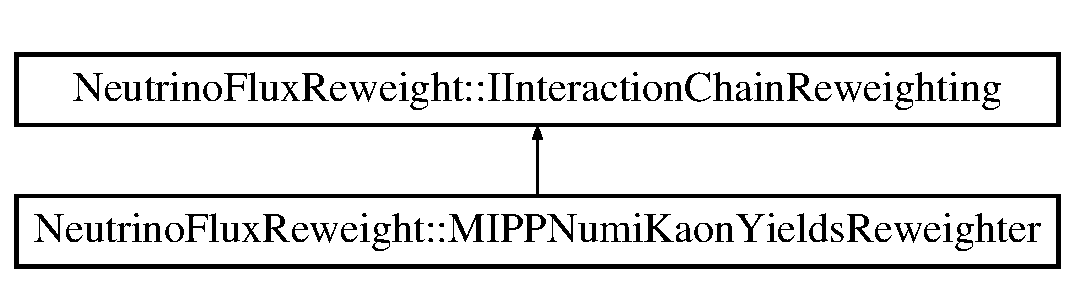
\includegraphics[height=2.000000cm]{class_neutrino_flux_reweight_1_1_m_i_p_p_numi_kaon_yields_reweighter}
\end{center}
\end{figure}
\subsection*{Public Member Functions}
\begin{DoxyCompactItemize}
\item 
\hyperlink{class_neutrino_flux_reweight_1_1_m_i_p_p_numi_kaon_yields_reweighter_ae0efdd82f42923c1ffdd2a7f8d4213e5}{M\-I\-P\-P\-Numi\-Kaon\-Yields\-Reweighter} (int iuniv, const \hyperlink{class_neutrino_flux_reweight_1_1_parameter_table}{Parameter\-Table} \&cv\-\_\-pars, const \hyperlink{class_neutrino_flux_reweight_1_1_parameter_table}{Parameter\-Table} \&univ\-\_\-pars)
\item 
virtual \hyperlink{class_neutrino_flux_reweight_1_1_m_i_p_p_numi_kaon_yields_reweighter_a9d49b5825c71d0ac29db896934f5cb77}{$\sim$\-M\-I\-P\-P\-Numi\-Kaon\-Yields\-Reweighter} ()
\item 
virtual std\-::vector$<$ bool $>$ \hyperlink{class_neutrino_flux_reweight_1_1_m_i_p_p_numi_kaon_yields_reweighter_a6ca3bcd0846fd600f51988a2e396aafb}{can\-Reweight} (const \hyperlink{class_neutrino_flux_reweight_1_1_interaction_chain_data}{Interaction\-Chain\-Data} \&aa)
\begin{DoxyCompactList}\small\item\em Look through the \hyperlink{class_neutrino_flux_reweight_1_1_interaction_chain_data}{Interaction\-Chain\-Data} input and identify those Interactions that can be reweighted as part of a chain. We return a vector indicating which elements will be assigned a weight by calculate\-Weight. \end{DoxyCompactList}\item 
virtual double \hyperlink{class_neutrino_flux_reweight_1_1_m_i_p_p_numi_kaon_yields_reweighter_ad9503e13848e30f432c297ed70e24134}{calculate\-Weight} (const \hyperlink{class_neutrino_flux_reweight_1_1_interaction_chain_data}{Interaction\-Chain\-Data} \&aa)
\begin{DoxyCompactList}\small\item\em calculate a weight for this interaction chain given the central value parameters and the parameters for this universe. The weight is something like\-: f(cv)/f(M\-C) $\ast$ f(univ)/f(cv) where cv in this case corresponds to the best value of the parameter, given the data. If univ\-\_\-pars=cv\-\_\-pars then we are calculating a central value weight. Note, \hyperlink{class_neutrino_flux_reweight_1_1_m_i_p_p_numi_kaon_yields_reweighter_a6ca3bcd0846fd600f51988a2e396aafb}{can\-Reweight()} should be called to determine which elements of the chain are covered by the weight returned by \hyperlink{class_neutrino_flux_reweight_1_1_m_i_p_p_numi_kaon_yields_reweighter_ad9503e13848e30f432c297ed70e24134}{calculate\-Weight()} \end{DoxyCompactList}\end{DoxyCompactItemize}
\subsection*{Public Attributes}
\begin{DoxyCompactItemize}
\item 
const \hyperlink{class_neutrino_flux_reweight_1_1_parameter_table}{Parameter\-Table} \& \hyperlink{class_neutrino_flux_reweight_1_1_m_i_p_p_numi_kaon_yields_reweighter_a39b091512948ed98beae0d341efa6d23}{cv\-Pars}
\item 
const \hyperlink{class_neutrino_flux_reweight_1_1_parameter_table}{Parameter\-Table} \& \hyperlink{class_neutrino_flux_reweight_1_1_m_i_p_p_numi_kaon_yields_reweighter_aef5aab54416e696526aa8ae2c92d1fd8}{univ\-Pars}
\end{DoxyCompactItemize}
\subsection*{Private Attributes}
\begin{DoxyCompactItemize}
\item 
int \hyperlink{class_neutrino_flux_reweight_1_1_m_i_p_p_numi_kaon_yields_reweighter_a22da7248cf883c4d01c486e6763dd3bc}{i\-Univ}
\item 
float \hyperlink{class_neutrino_flux_reweight_1_1_m_i_p_p_numi_kaon_yields_reweighter_ad0e1b0e610a8d647d0be6d97e80327fa}{prt\-\_\-no\-\_\-inter}
\item 
std\-::vector$<$ float $>$ \hyperlink{class_neutrino_flux_reweight_1_1_m_i_p_p_numi_kaon_yields_reweighter_a826bd079aef8a6915cea2dd8ccf03589}{vbin\-\_\-datacv\-\_\-pip}
\item 
std\-::vector$<$ float $>$ \hyperlink{class_neutrino_flux_reweight_1_1_m_i_p_p_numi_kaon_yields_reweighter_a5c434b561304af4dd8d0a5145b07b62e}{vbin\-\_\-datacv\-\_\-pim}
\item 
std\-::vector$<$ float $>$ \hyperlink{class_neutrino_flux_reweight_1_1_m_i_p_p_numi_kaon_yields_reweighter_a852ed8a2467fade867ca8abe0d0b3037}{vbin\-\_\-datasys\-\_\-pip}
\item 
std\-::vector$<$ float $>$ \hyperlink{class_neutrino_flux_reweight_1_1_m_i_p_p_numi_kaon_yields_reweighter_a1c50c5dbfbf3688e4034dead330d83db}{vbin\-\_\-datasys\-\_\-pim}
\item 
std\-::vector$<$ float $>$ \hyperlink{class_neutrino_flux_reweight_1_1_m_i_p_p_numi_kaon_yields_reweighter_a258a6c0170a0ba06b44fad43b7dcff2f}{vbin\-\_\-datasta\-\_\-pip}
\item 
std\-::vector$<$ float $>$ \hyperlink{class_neutrino_flux_reweight_1_1_m_i_p_p_numi_kaon_yields_reweighter_aada860b3db9a168dcfda7a2df361591e}{vbin\-\_\-datasta\-\_\-pim}
\item 
std\-::vector$<$ float $>$ \hyperlink{class_neutrino_flux_reweight_1_1_m_i_p_p_numi_kaon_yields_reweighter_a1d8321111a686ae97238fb98ed7c1a1b}{vbin\-\_\-datacv\-\_\-kap\-\_\-pip}
\item 
std\-::vector$<$ float $>$ \hyperlink{class_neutrino_flux_reweight_1_1_m_i_p_p_numi_kaon_yields_reweighter_a862186e4424a3514fc7441fc40bb2be3}{vbin\-\_\-datacv\-\_\-kam\-\_\-pim}
\item 
std\-::vector$<$ float $>$ \hyperlink{class_neutrino_flux_reweight_1_1_m_i_p_p_numi_kaon_yields_reweighter_a7a026f18f2ee99ed16e5dd2bdb5c96af}{vbin\-\_\-datasys\-\_\-kap\-\_\-pip}
\item 
std\-::vector$<$ float $>$ \hyperlink{class_neutrino_flux_reweight_1_1_m_i_p_p_numi_kaon_yields_reweighter_a26e3d74e529b8d9f359b1f6501665178}{vbin\-\_\-datasys\-\_\-kam\-\_\-pim}
\item 
std\-::vector$<$ float $>$ \hyperlink{class_neutrino_flux_reweight_1_1_m_i_p_p_numi_kaon_yields_reweighter_a014b0274aeb81973cc0579c218709031}{vbin\-\_\-datasta\-\_\-kap\-\_\-pip}
\item 
std\-::vector$<$ float $>$ \hyperlink{class_neutrino_flux_reweight_1_1_m_i_p_p_numi_kaon_yields_reweighter_adbfd90fe79b72cba9a772bb563f7e4fa}{vbin\-\_\-datasta\-\_\-kam\-\_\-pim}
\item 
float \hyperlink{class_neutrino_flux_reweight_1_1_m_i_p_p_numi_kaon_yields_reweighter_a834bede67f164f8a08d50bd15f8ef02c}{aux\-\_\-par}
\end{DoxyCompactItemize}


\subsection{Detailed Description}
Reweight a chain of interactions that are covered by the Nu\-M\-I target K/pi ratios measured by M\-I\-P\-P. 

Definition at line 15 of file M\-I\-P\-P\-Numi\-Kaon\-Yields\-Reweighter.\-h.



\subsection{Constructor \& Destructor Documentation}
\hypertarget{class_neutrino_flux_reweight_1_1_m_i_p_p_numi_kaon_yields_reweighter_ae0efdd82f42923c1ffdd2a7f8d4213e5}{\index{Neutrino\-Flux\-Reweight\-::\-M\-I\-P\-P\-Numi\-Kaon\-Yields\-Reweighter@{Neutrino\-Flux\-Reweight\-::\-M\-I\-P\-P\-Numi\-Kaon\-Yields\-Reweighter}!M\-I\-P\-P\-Numi\-Kaon\-Yields\-Reweighter@{M\-I\-P\-P\-Numi\-Kaon\-Yields\-Reweighter}}
\index{M\-I\-P\-P\-Numi\-Kaon\-Yields\-Reweighter@{M\-I\-P\-P\-Numi\-Kaon\-Yields\-Reweighter}!NeutrinoFluxReweight::MIPPNumiKaonYieldsReweighter@{Neutrino\-Flux\-Reweight\-::\-M\-I\-P\-P\-Numi\-Kaon\-Yields\-Reweighter}}
\subsubsection[{M\-I\-P\-P\-Numi\-Kaon\-Yields\-Reweighter}]{\setlength{\rightskip}{0pt plus 5cm}Neutrino\-Flux\-Reweight\-::\-M\-I\-P\-P\-Numi\-Kaon\-Yields\-Reweighter\-::\-M\-I\-P\-P\-Numi\-Kaon\-Yields\-Reweighter (
\begin{DoxyParamCaption}
\item[{int}]{iuniv, }
\item[{const {\bf Parameter\-Table} \&}]{cv\-\_\-pars, }
\item[{const {\bf Parameter\-Table} \&}]{univ\-\_\-pars}
\end{DoxyParamCaption}
)}}\label{class_neutrino_flux_reweight_1_1_m_i_p_p_numi_kaon_yields_reweighter_ae0efdd82f42923c1ffdd2a7f8d4213e5}
The constructor. Note, we pass central value and single universe parameters in this constructor only. There is thus a 1 to 1 correspondence between an instance of this class and a given universe. 

Definition at line 11 of file M\-I\-P\-P\-Numi\-Kaon\-Yields\-Reweighter.\-cpp.


\begin{DoxyCode}
11                                                                                                            
                                : \hyperlink{class_neutrino_flux_reweight_1_1_m_i_p_p_numi_kaon_yields_reweighter_a39b091512948ed98beae0d341efa6d23}{cvPars}(cv\_pars), \hyperlink{class_neutrino_flux_reweight_1_1_m_i_p_p_numi_kaon_yields_reweighter_aef5aab54416e696526aa8ae2c92d1fd8}{univPars}(univ\_pars), 
      \hyperlink{class_neutrino_flux_reweight_1_1_m_i_p_p_numi_kaon_yields_reweighter_a22da7248cf883c4d01c486e6763dd3bc}{iUniv}(iuniv)\{
12     
13     MIPPNumiYieldsBins* MIPPbins =  \hyperlink{class_neutrino_flux_reweight_1_1_m_i_p_p_numi_yields_bins_a7f44afe90a846812d6eabfafa8f576e4}{MIPPNumiYieldsBins::getInstance}();
14     \hyperlink{class_neutrino_flux_reweight_1_1_m_i_p_p_numi_kaon_yields_reweighter_a826bd079aef8a6915cea2dd8ccf03589}{vbin\_datacv\_pip}.reserve(MIPPbins->GetNbins\_pip\_MIPPNuMI());
15     \hyperlink{class_neutrino_flux_reweight_1_1_m_i_p_p_numi_kaon_yields_reweighter_a5c434b561304af4dd8d0a5145b07b62e}{vbin\_datacv\_pim}.reserve(MIPPbins->GetNbins\_pim\_MIPPNuMI());
16     \hyperlink{class_neutrino_flux_reweight_1_1_m_i_p_p_numi_kaon_yields_reweighter_a852ed8a2467fade867ca8abe0d0b3037}{vbin\_datasys\_pip}.reserve(MIPPbins->GetNbins\_pip\_MIPPNuMI());
17     \hyperlink{class_neutrino_flux_reweight_1_1_m_i_p_p_numi_kaon_yields_reweighter_a1c50c5dbfbf3688e4034dead330d83db}{vbin\_datasys\_pim}.reserve(MIPPbins->GetNbins\_pim\_MIPPNuMI());
18     \hyperlink{class_neutrino_flux_reweight_1_1_m_i_p_p_numi_kaon_yields_reweighter_a258a6c0170a0ba06b44fad43b7dcff2f}{vbin\_datasta\_pip}.reserve(MIPPbins->GetNbins\_pip\_MIPPNuMI());
19     \hyperlink{class_neutrino_flux_reweight_1_1_m_i_p_p_numi_kaon_yields_reweighter_aada860b3db9a168dcfda7a2df361591e}{vbin\_datasta\_pim}.reserve(MIPPbins->GetNbins\_pim\_MIPPNuMI());
20     
21     \hyperlink{class_neutrino_flux_reweight_1_1_m_i_p_p_numi_kaon_yields_reweighter_a1d8321111a686ae97238fb98ed7c1a1b}{vbin\_datacv\_kap\_pip}.reserve(MIPPbins->GetNbins\_K\_MIPPNuMI());
22     \hyperlink{class_neutrino_flux_reweight_1_1_m_i_p_p_numi_kaon_yields_reweighter_a862186e4424a3514fc7441fc40bb2be3}{vbin\_datacv\_kam\_pim}.reserve(MIPPbins->GetNbins\_K\_MIPPNuMI());
23     \hyperlink{class_neutrino_flux_reweight_1_1_m_i_p_p_numi_kaon_yields_reweighter_a7a026f18f2ee99ed16e5dd2bdb5c96af}{vbin\_datasys\_kap\_pip}.reserve(MIPPbins->GetNbins\_K\_MIPPNuMI());
24     \hyperlink{class_neutrino_flux_reweight_1_1_m_i_p_p_numi_kaon_yields_reweighter_a26e3d74e529b8d9f359b1f6501665178}{vbin\_datasys\_kam\_pim}.reserve(MIPPbins->GetNbins\_K\_MIPPNuMI());
25     \hyperlink{class_neutrino_flux_reweight_1_1_m_i_p_p_numi_kaon_yields_reweighter_a014b0274aeb81973cc0579c218709031}{vbin\_datasta\_kap\_pip}.reserve(MIPPbins->GetNbins\_K\_MIPPNuMI());
26     \hyperlink{class_neutrino_flux_reweight_1_1_m_i_p_p_numi_kaon_yields_reweighter_adbfd90fe79b72cba9a772bb563f7e4fa}{vbin\_datasta\_kam\_pim}.reserve(MIPPbins->GetNbins\_K\_MIPPNuMI());
27 
28     \textcolor{comment}{//const boost::interprocess::flat\_map<std::string, double>& univ\_table = univPars.getMap();}
29     \textcolor{comment}{//const boost::interprocess::flat\_map<std::string, double>& cv\_table = cvPars.getMap();}
30      \hyperlink{class_neutrino_flux_reweight_1_1_m_i_p_p_numi_kaon_yields_reweighter_ad0e1b0e610a8d647d0be6d97e80327fa}{prt\_no\_inter} = \hyperlink{class_neutrino_flux_reweight_1_1_m_i_p_p_numi_kaon_yields_reweighter_aef5aab54416e696526aa8ae2c92d1fd8}{univPars}.\hyperlink{class_neutrino_flux_reweight_1_1_parameter_table_acb7dc8335b65b116f6092f2fa57ca5ed}{getParameterValue}(\textcolor{stringliteral}{"prt\_no\_interacting"});
31      
32      \textcolor{keywordtype}{char} namepar[100];
33      \textcolor{keywordflow}{for}(\textcolor{keywordtype}{int} ii=0;ii<MIPPbins->GetNbins\_pip\_MIPPNuMI();ii++)\{
34       sprintf(namepar,\textcolor{stringliteral}{"MIPP\_NuMI\_%s\_sys\_%d"},\textcolor{stringliteral}{"pip"},ii);
35       \textcolor{keywordtype}{double} data\_cv  = \hyperlink{class_neutrino_flux_reweight_1_1_m_i_p_p_numi_kaon_yields_reweighter_a39b091512948ed98beae0d341efa6d23}{cvPars}.\hyperlink{class_neutrino_flux_reweight_1_1_parameter_table_acb7dc8335b65b116f6092f2fa57ca5ed}{getParameterValue}(std::string(namepar));
36       \textcolor{keywordtype}{double} data\_sys = \hyperlink{class_neutrino_flux_reweight_1_1_m_i_p_p_numi_kaon_yields_reweighter_aef5aab54416e696526aa8ae2c92d1fd8}{univPars}.\hyperlink{class_neutrino_flux_reweight_1_1_parameter_table_acb7dc8335b65b116f6092f2fa57ca5ed}{getParameterValue}(std::string(namepar));
37       sprintf(namepar,\textcolor{stringliteral}{"MIPP\_NuMI\_%s\_stats\_%d"},\textcolor{stringliteral}{"pip"},ii);
38       \textcolor{keywordtype}{double} data\_sta = \hyperlink{class_neutrino_flux_reweight_1_1_m_i_p_p_numi_kaon_yields_reweighter_aef5aab54416e696526aa8ae2c92d1fd8}{univPars}.\hyperlink{class_neutrino_flux_reweight_1_1_parameter_table_acb7dc8335b65b116f6092f2fa57ca5ed}{getParameterValue}(std::string(namepar));
39       data\_sys /= (1.0-\hyperlink{class_neutrino_flux_reweight_1_1_m_i_p_p_numi_kaon_yields_reweighter_ad0e1b0e610a8d647d0be6d97e80327fa}{prt\_no\_inter});
40       data\_sta /= (1.0-\hyperlink{class_neutrino_flux_reweight_1_1_m_i_p_p_numi_kaon_yields_reweighter_ad0e1b0e610a8d647d0be6d97e80327fa}{prt\_no\_inter});
41       data\_cv  /= (1.0-\hyperlink{class_neutrino_flux_reweight_1_1_m_i_p_p_numi_kaon_yields_reweighter_ad0e1b0e610a8d647d0be6d97e80327fa}{prt\_no\_inter});
42       \hyperlink{class_neutrino_flux_reweight_1_1_m_i_p_p_numi_kaon_yields_reweighter_a826bd079aef8a6915cea2dd8ccf03589}{vbin\_datacv\_pip}.push\_back(data\_cv);
43       \hyperlink{class_neutrino_flux_reweight_1_1_m_i_p_p_numi_kaon_yields_reweighter_a852ed8a2467fade867ca8abe0d0b3037}{vbin\_datasys\_pip}.push\_back(data\_sys);
44       \hyperlink{class_neutrino_flux_reweight_1_1_m_i_p_p_numi_kaon_yields_reweighter_a258a6c0170a0ba06b44fad43b7dcff2f}{vbin\_datasta\_pip}.push\_back(data\_sta);
45      \}
46      
47      \textcolor{keywordflow}{for}(\textcolor{keywordtype}{int} ii=0;ii<MIPPbins->GetNbins\_pim\_MIPPNuMI();ii++)\{
48       sprintf(namepar,\textcolor{stringliteral}{"MIPP\_NuMI\_%s\_sys\_%d"},\textcolor{stringliteral}{"pim"},ii);
49       \textcolor{keywordtype}{double} data\_cv  = \hyperlink{class_neutrino_flux_reweight_1_1_m_i_p_p_numi_kaon_yields_reweighter_a39b091512948ed98beae0d341efa6d23}{cvPars}.\hyperlink{class_neutrino_flux_reweight_1_1_parameter_table_acb7dc8335b65b116f6092f2fa57ca5ed}{getParameterValue}(std::string(namepar));
50       \textcolor{keywordtype}{double} data\_sys = \hyperlink{class_neutrino_flux_reweight_1_1_m_i_p_p_numi_kaon_yields_reweighter_aef5aab54416e696526aa8ae2c92d1fd8}{univPars}.\hyperlink{class_neutrino_flux_reweight_1_1_parameter_table_acb7dc8335b65b116f6092f2fa57ca5ed}{getParameterValue}(std::string(namepar));
51       sprintf(namepar,\textcolor{stringliteral}{"MIPP\_NuMI\_%s\_stats\_%d"},\textcolor{stringliteral}{"pim"},ii);
52       \textcolor{keywordtype}{double} data\_sta = \hyperlink{class_neutrino_flux_reweight_1_1_m_i_p_p_numi_kaon_yields_reweighter_aef5aab54416e696526aa8ae2c92d1fd8}{univPars}.\hyperlink{class_neutrino_flux_reweight_1_1_parameter_table_acb7dc8335b65b116f6092f2fa57ca5ed}{getParameterValue}(std::string(namepar));
53       data\_sys /= (1.0-\hyperlink{class_neutrino_flux_reweight_1_1_m_i_p_p_numi_kaon_yields_reweighter_ad0e1b0e610a8d647d0be6d97e80327fa}{prt\_no\_inter});
54       data\_sta /= (1.0-\hyperlink{class_neutrino_flux_reweight_1_1_m_i_p_p_numi_kaon_yields_reweighter_ad0e1b0e610a8d647d0be6d97e80327fa}{prt\_no\_inter});
55       data\_cv  /= (1.0-\hyperlink{class_neutrino_flux_reweight_1_1_m_i_p_p_numi_kaon_yields_reweighter_ad0e1b0e610a8d647d0be6d97e80327fa}{prt\_no\_inter});
56       \hyperlink{class_neutrino_flux_reweight_1_1_m_i_p_p_numi_kaon_yields_reweighter_a5c434b561304af4dd8d0a5145b07b62e}{vbin\_datacv\_pim}.push\_back(data\_cv);
57       \hyperlink{class_neutrino_flux_reweight_1_1_m_i_p_p_numi_kaon_yields_reweighter_a1c50c5dbfbf3688e4034dead330d83db}{vbin\_datasys\_pim}.push\_back(data\_sys);
58       \hyperlink{class_neutrino_flux_reweight_1_1_m_i_p_p_numi_kaon_yields_reweighter_aada860b3db9a168dcfda7a2df361591e}{vbin\_datasta\_pim}.push\_back(data\_sta);
59      \}
60     \textcolor{keywordflow}{for}(\textcolor{keywordtype}{int} ii=0;ii<MIPPbins->GetNbins\_K\_MIPPNuMI();ii++)\{
61       sprintf(namepar,\textcolor{stringliteral}{"MIPP\_NuMI\_%s\_sys\_%d"},\textcolor{stringliteral}{"kap\_pip"},ii);
62       \textcolor{keywordtype}{double} data\_cv  = \hyperlink{class_neutrino_flux_reweight_1_1_m_i_p_p_numi_kaon_yields_reweighter_a39b091512948ed98beae0d341efa6d23}{cvPars}.\hyperlink{class_neutrino_flux_reweight_1_1_parameter_table_acb7dc8335b65b116f6092f2fa57ca5ed}{getParameterValue}(std::string(namepar));
63       \textcolor{keywordtype}{double} data\_sys = \hyperlink{class_neutrino_flux_reweight_1_1_m_i_p_p_numi_kaon_yields_reweighter_aef5aab54416e696526aa8ae2c92d1fd8}{univPars}.\hyperlink{class_neutrino_flux_reweight_1_1_parameter_table_acb7dc8335b65b116f6092f2fa57ca5ed}{getParameterValue}(std::string(namepar));
64       sprintf(namepar,\textcolor{stringliteral}{"MIPP\_NuMI\_%s\_stats\_%d"},\textcolor{stringliteral}{"kap\_pip"},ii);
65       \textcolor{keywordtype}{double} data\_sta = \hyperlink{class_neutrino_flux_reweight_1_1_m_i_p_p_numi_kaon_yields_reweighter_aef5aab54416e696526aa8ae2c92d1fd8}{univPars}.\hyperlink{class_neutrino_flux_reweight_1_1_parameter_table_acb7dc8335b65b116f6092f2fa57ca5ed}{getParameterValue}(std::string(namepar));
66       \hyperlink{class_neutrino_flux_reweight_1_1_m_i_p_p_numi_kaon_yields_reweighter_a1d8321111a686ae97238fb98ed7c1a1b}{vbin\_datacv\_kap\_pip}.push\_back(data\_cv);
67       \hyperlink{class_neutrino_flux_reweight_1_1_m_i_p_p_numi_kaon_yields_reweighter_a7a026f18f2ee99ed16e5dd2bdb5c96af}{vbin\_datasys\_kap\_pip}.push\_back(data\_sys);
68       \hyperlink{class_neutrino_flux_reweight_1_1_m_i_p_p_numi_kaon_yields_reweighter_a014b0274aeb81973cc0579c218709031}{vbin\_datasta\_kap\_pip}.push\_back(data\_sta);
69       
70       sprintf(namepar,\textcolor{stringliteral}{"MIPP\_NuMI\_%s\_sys\_%d"},\textcolor{stringliteral}{"kam\_pim"},ii);
71       data\_cv  = \hyperlink{class_neutrino_flux_reweight_1_1_m_i_p_p_numi_kaon_yields_reweighter_a39b091512948ed98beae0d341efa6d23}{cvPars}.\hyperlink{class_neutrino_flux_reweight_1_1_parameter_table_acb7dc8335b65b116f6092f2fa57ca5ed}{getParameterValue}(std::string(namepar));
72       data\_sys = \hyperlink{class_neutrino_flux_reweight_1_1_m_i_p_p_numi_kaon_yields_reweighter_aef5aab54416e696526aa8ae2c92d1fd8}{univPars}.\hyperlink{class_neutrino_flux_reweight_1_1_parameter_table_acb7dc8335b65b116f6092f2fa57ca5ed}{getParameterValue}(std::string(namepar));
73       sprintf(namepar,\textcolor{stringliteral}{"MIPP\_NuMI\_%s\_stats\_%d"},\textcolor{stringliteral}{"kam\_pim"},ii);
74       data\_sta = \hyperlink{class_neutrino_flux_reweight_1_1_m_i_p_p_numi_kaon_yields_reweighter_aef5aab54416e696526aa8ae2c92d1fd8}{univPars}.\hyperlink{class_neutrino_flux_reweight_1_1_parameter_table_acb7dc8335b65b116f6092f2fa57ca5ed}{getParameterValue}(std::string(namepar));
75       \hyperlink{class_neutrino_flux_reweight_1_1_m_i_p_p_numi_kaon_yields_reweighter_a862186e4424a3514fc7441fc40bb2be3}{vbin\_datacv\_kam\_pim}.push\_back(data\_cv);
76       \hyperlink{class_neutrino_flux_reweight_1_1_m_i_p_p_numi_kaon_yields_reweighter_a26e3d74e529b8d9f359b1f6501665178}{vbin\_datasys\_kam\_pim}.push\_back(data\_sys);
77       \hyperlink{class_neutrino_flux_reweight_1_1_m_i_p_p_numi_kaon_yields_reweighter_adbfd90fe79b72cba9a772bb563f7e4fa}{vbin\_datasta\_kam\_pim}.push\_back(data\_sta);
78     \} 
79     \hyperlink{class_neutrino_flux_reweight_1_1_m_i_p_p_numi_kaon_yields_reweighter_a834bede67f164f8a08d50bd15f8ef02c}{aux\_par} = \hyperlink{class_neutrino_flux_reweight_1_1_m_i_p_p_numi_kaon_yields_reweighter_aef5aab54416e696526aa8ae2c92d1fd8}{univPars}.\hyperlink{class_neutrino_flux_reweight_1_1_parameter_table_acb7dc8335b65b116f6092f2fa57ca5ed}{getParameterValue}(\textcolor{stringliteral}{"aux\_parameter"});
80     \textcolor{keywordflow}{if}(\hyperlink{class_neutrino_flux_reweight_1_1_m_i_p_p_numi_kaon_yields_reweighter_a834bede67f164f8a08d50bd15f8ef02c}{aux\_par}<1.e-15)\hyperlink{class_neutrino_flux_reweight_1_1_m_i_p_p_numi_kaon_yields_reweighter_a834bede67f164f8a08d50bd15f8ef02c}{aux\_par} = 1.0;
81     
82   \}
\end{DoxyCode}
\hypertarget{class_neutrino_flux_reweight_1_1_m_i_p_p_numi_kaon_yields_reweighter_a9d49b5825c71d0ac29db896934f5cb77}{\index{Neutrino\-Flux\-Reweight\-::\-M\-I\-P\-P\-Numi\-Kaon\-Yields\-Reweighter@{Neutrino\-Flux\-Reweight\-::\-M\-I\-P\-P\-Numi\-Kaon\-Yields\-Reweighter}!$\sim$\-M\-I\-P\-P\-Numi\-Kaon\-Yields\-Reweighter@{$\sim$\-M\-I\-P\-P\-Numi\-Kaon\-Yields\-Reweighter}}
\index{$\sim$\-M\-I\-P\-P\-Numi\-Kaon\-Yields\-Reweighter@{$\sim$\-M\-I\-P\-P\-Numi\-Kaon\-Yields\-Reweighter}!NeutrinoFluxReweight::MIPPNumiKaonYieldsReweighter@{Neutrino\-Flux\-Reweight\-::\-M\-I\-P\-P\-Numi\-Kaon\-Yields\-Reweighter}}
\subsubsection[{$\sim$\-M\-I\-P\-P\-Numi\-Kaon\-Yields\-Reweighter}]{\setlength{\rightskip}{0pt plus 5cm}Neutrino\-Flux\-Reweight\-::\-M\-I\-P\-P\-Numi\-Kaon\-Yields\-Reweighter\-::$\sim$\-M\-I\-P\-P\-Numi\-Kaon\-Yields\-Reweighter (
\begin{DoxyParamCaption}
{}
\end{DoxyParamCaption}
)\hspace{0.3cm}{\ttfamily [virtual]}}}\label{class_neutrino_flux_reweight_1_1_m_i_p_p_numi_kaon_yields_reweighter_a9d49b5825c71d0ac29db896934f5cb77}


Definition at line 83 of file M\-I\-P\-P\-Numi\-Kaon\-Yields\-Reweighter.\-cpp.


\begin{DoxyCode}
83                                                              \{
84     
85   \}
\end{DoxyCode}


\subsection{Member Function Documentation}
\hypertarget{class_neutrino_flux_reweight_1_1_m_i_p_p_numi_kaon_yields_reweighter_ad9503e13848e30f432c297ed70e24134}{\index{Neutrino\-Flux\-Reweight\-::\-M\-I\-P\-P\-Numi\-Kaon\-Yields\-Reweighter@{Neutrino\-Flux\-Reweight\-::\-M\-I\-P\-P\-Numi\-Kaon\-Yields\-Reweighter}!calculate\-Weight@{calculate\-Weight}}
\index{calculate\-Weight@{calculate\-Weight}!NeutrinoFluxReweight::MIPPNumiKaonYieldsReweighter@{Neutrino\-Flux\-Reweight\-::\-M\-I\-P\-P\-Numi\-Kaon\-Yields\-Reweighter}}
\subsubsection[{calculate\-Weight}]{\setlength{\rightskip}{0pt plus 5cm}double Neutrino\-Flux\-Reweight\-::\-M\-I\-P\-P\-Numi\-Kaon\-Yields\-Reweighter\-::calculate\-Weight (
\begin{DoxyParamCaption}
\item[{const {\bf Interaction\-Chain\-Data} \&}]{aa}
\end{DoxyParamCaption}
)\hspace{0.3cm}{\ttfamily [virtual]}}}\label{class_neutrino_flux_reweight_1_1_m_i_p_p_numi_kaon_yields_reweighter_ad9503e13848e30f432c297ed70e24134}


calculate a weight for this interaction chain given the central value parameters and the parameters for this universe. The weight is something like\-: f(cv)/f(M\-C) $\ast$ f(univ)/f(cv) where cv in this case corresponds to the best value of the parameter, given the data. If univ\-\_\-pars=cv\-\_\-pars then we are calculating a central value weight. Note, \hyperlink{class_neutrino_flux_reweight_1_1_m_i_p_p_numi_kaon_yields_reweighter_a6ca3bcd0846fd600f51988a2e396aafb}{can\-Reweight()} should be called to determine which elements of the chain are covered by the weight returned by \hyperlink{class_neutrino_flux_reweight_1_1_m_i_p_p_numi_kaon_yields_reweighter_ad9503e13848e30f432c297ed70e24134}{calculate\-Weight()} 



Implements \hyperlink{class_neutrino_flux_reweight_1_1_i_interaction_chain_reweighting_ae28403553637013fdc720674ee24c7c5}{Neutrino\-Flux\-Reweight\-::\-I\-Interaction\-Chain\-Reweighting}.



Definition at line 135 of file M\-I\-P\-P\-Numi\-Kaon\-Yields\-Reweighter.\-cpp.


\begin{DoxyCode}
135                                                                                     \{
136     
137     \textcolor{keywordtype}{double} wgt = 1.0;
138 
139     MIPPNumiYieldsBins*  MIPPbins =  \hyperlink{class_neutrino_flux_reweight_1_1_m_i_p_p_numi_yields_bins_a7f44afe90a846812d6eabfafa8f576e4}{MIPPNumiYieldsBins::getInstance}();
140     MIPPNumiMC*  MCval =  \hyperlink{class_neutrino_flux_reweight_1_1_m_i_p_p_numi_m_c_a4324da8640cc9a0d157d82e08da3a1c3}{MIPPNumiMC::getInstance}();
141     \textcolor{keywordtype}{double} low\_value = 1.e-18;      
142     
143     TargetData tar = aa.tar\_info;
144 
145     \textcolor{comment}{//fast check:}
146     \textcolor{keywordflow}{if}(tar.Tar\_pdg != 321 && tar.Tar\_pdg != -321 && tar.Tar\_pdg != 130 && tar.Tar\_pdg != 310)\textcolor{keywordflow}{return} 
      \hyperlink{class_neutrino_flux_reweight_1_1_m_i_p_p_numi_kaon_yields_reweighter_a834bede67f164f8a08d50bd15f8ef02c}{aux\_par};
147     \textcolor{keywordflow}{if}(tar.Pz<20.0 || tar.Pz>80.0 || tar.Pt>2.0)\textcolor{keywordflow}{return} \hyperlink{class_neutrino_flux_reweight_1_1_m_i_p_p_numi_kaon_yields_reweighter_a834bede67f164f8a08d50bd15f8ef02c}{aux\_par};
148     \textcolor{keywordtype}{int} binID = MIPPbins->BinID(tar.Pz,tar.Pt,tar.Tar\_pdg);
149     \textcolor{keywordflow}{if}(binID<0)\{
150       \textcolor{keywordflow}{return} \hyperlink{class_neutrino_flux_reweight_1_1_m_i_p_p_numi_kaon_yields_reweighter_a834bede67f164f8a08d50bd15f8ef02c}{aux\_par};
151     \}
152     \textcolor{comment}{//Now looking for pions bin ID:}
153     \textcolor{keywordtype}{int} pip\_bin = MIPPbins->BinID(tar.Pz,tar.Pt, 211);
154     \textcolor{keywordtype}{int} pim\_bin = MIPPbins->BinID(tar.Pz,tar.Pt,-211);
155     \textcolor{keywordflow}{if}(tar.Tar\_pdg == 321 && pip\_bin<0)\textcolor{keywordflow}{return} \hyperlink{class_neutrino_flux_reweight_1_1_m_i_p_p_numi_kaon_yields_reweighter_a834bede67f164f8a08d50bd15f8ef02c}{aux\_par};
156     \textcolor{keywordflow}{if}(tar.Tar\_pdg ==-321 && pim\_bin<0)\textcolor{keywordflow}{return} \hyperlink{class_neutrino_flux_reweight_1_1_m_i_p_p_numi_kaon_yields_reweighter_a834bede67f164f8a08d50bd15f8ef02c}{aux\_par};
157     \textcolor{keywordflow}{if}(tar.Tar\_pdg == 130 || tar.Tar\_pdg == 310)\{
158       \textcolor{keywordflow}{if}(pip\_bin<0 || pim\_bin<0)\textcolor{keywordflow}{return} \hyperlink{class_neutrino_flux_reweight_1_1_m_i_p_p_numi_kaon_yields_reweighter_a834bede67f164f8a08d50bd15f8ef02c}{aux\_par};
159     \}
160     
161     \textcolor{comment}{//Now, looking for the MC value:}
162     \textcolor{keywordtype}{double} binC = MCval->getMCval(tar.Pz,tar.Pt,tar.Tar\_pdg);
163     \textcolor{keywordflow}{if}(binC<low\_value)\{
164       \textcolor{comment}{//std::cout<<"LOW MC VAL: "<<binC <<std::endl;}
165       \textcolor{keywordflow}{return} \hyperlink{class_neutrino_flux_reweight_1_1_m_i_p_p_numi_kaon_yields_reweighter_a834bede67f164f8a08d50bd15f8ef02c}{aux\_par};
166     \}
167 
168     \textcolor{keywordtype}{float} K\_data\_cv  = -1.0;
169     \textcolor{keywordtype}{float} K\_data\_sys = -1.0;
170     \textcolor{keywordtype}{float} K\_data\_sta = -1.0;
171     \textcolor{keywordtype}{float} K\_data     = -1.0;
172     \textcolor{keywordtype}{float} K\_aux      = -1.0;
173     
174     \textcolor{keywordflow}{if}(tar.Tar\_pdg == 321)\{
175       K\_data\_cv  = \hyperlink{class_neutrino_flux_reweight_1_1_m_i_p_p_numi_kaon_yields_reweighter_a826bd079aef8a6915cea2dd8ccf03589}{vbin\_datacv\_pip}[pip\_bin] *\hyperlink{class_neutrino_flux_reweight_1_1_m_i_p_p_numi_kaon_yields_reweighter_a1d8321111a686ae97238fb98ed7c1a1b}{vbin\_datacv\_kap\_pip}[binID];
176       K\_data\_sys = \hyperlink{class_neutrino_flux_reweight_1_1_m_i_p_p_numi_kaon_yields_reweighter_a852ed8a2467fade867ca8abe0d0b3037}{vbin\_datasys\_pip}[pip\_bin]*
      \hyperlink{class_neutrino_flux_reweight_1_1_m_i_p_p_numi_kaon_yields_reweighter_a7a026f18f2ee99ed16e5dd2bdb5c96af}{vbin\_datasys\_kap\_pip}[binID];
177       K\_data\_sta = \hyperlink{class_neutrino_flux_reweight_1_1_m_i_p_p_numi_kaon_yields_reweighter_a258a6c0170a0ba06b44fad43b7dcff2f}{vbin\_datasta\_pip}[pip\_bin]*
      \hyperlink{class_neutrino_flux_reweight_1_1_m_i_p_p_numi_kaon_yields_reweighter_a014b0274aeb81973cc0579c218709031}{vbin\_datasta\_kap\_pip}[binID];
178       K\_data = K\_data\_sys + K\_data\_sta - K\_data\_cv;
179       
180     \}
181     \textcolor{keywordflow}{else} \textcolor{keywordflow}{if}(tar.Tar\_pdg ==-321)\{
182       K\_data\_cv  = \hyperlink{class_neutrino_flux_reweight_1_1_m_i_p_p_numi_kaon_yields_reweighter_a5c434b561304af4dd8d0a5145b07b62e}{vbin\_datacv\_pim}[pim\_bin] *\hyperlink{class_neutrino_flux_reweight_1_1_m_i_p_p_numi_kaon_yields_reweighter_a862186e4424a3514fc7441fc40bb2be3}{vbin\_datacv\_kam\_pim}[binID];
183       K\_data\_sys = \hyperlink{class_neutrino_flux_reweight_1_1_m_i_p_p_numi_kaon_yields_reweighter_a1c50c5dbfbf3688e4034dead330d83db}{vbin\_datasys\_pim}[pim\_bin]*
      \hyperlink{class_neutrino_flux_reweight_1_1_m_i_p_p_numi_kaon_yields_reweighter_a26e3d74e529b8d9f359b1f6501665178}{vbin\_datasys\_kam\_pim}[binID];
184       K\_data\_sta = \hyperlink{class_neutrino_flux_reweight_1_1_m_i_p_p_numi_kaon_yields_reweighter_aada860b3db9a168dcfda7a2df361591e}{vbin\_datasta\_pim}[pim\_bin]*
      \hyperlink{class_neutrino_flux_reweight_1_1_m_i_p_p_numi_kaon_yields_reweighter_adbfd90fe79b72cba9a772bb563f7e4fa}{vbin\_datasta\_kam\_pim}[binID];
185       K\_data = K\_data\_sys + K\_data\_sta - K\_data\_cv;
186     \}
187     \textcolor{keywordflow}{else} \textcolor{keywordflow}{if}(tar.Tar\_pdg ==310 || tar.Tar\_pdg ==130)\{
188       \textcolor{comment}{//pip:}
189       K\_data\_cv  = \hyperlink{class_neutrino_flux_reweight_1_1_m_i_p_p_numi_kaon_yields_reweighter_a826bd079aef8a6915cea2dd8ccf03589}{vbin\_datacv\_pip}[pip\_bin] *\hyperlink{class_neutrino_flux_reweight_1_1_m_i_p_p_numi_kaon_yields_reweighter_a1d8321111a686ae97238fb98ed7c1a1b}{vbin\_datacv\_kap\_pip}[binID];
190       K\_data\_sys = \hyperlink{class_neutrino_flux_reweight_1_1_m_i_p_p_numi_kaon_yields_reweighter_a852ed8a2467fade867ca8abe0d0b3037}{vbin\_datasys\_pip}[pip\_bin]*
      \hyperlink{class_neutrino_flux_reweight_1_1_m_i_p_p_numi_kaon_yields_reweighter_a7a026f18f2ee99ed16e5dd2bdb5c96af}{vbin\_datasys\_kap\_pip}[binID];
191       K\_data\_sta = \hyperlink{class_neutrino_flux_reweight_1_1_m_i_p_p_numi_kaon_yields_reweighter_a258a6c0170a0ba06b44fad43b7dcff2f}{vbin\_datasta\_pip}[pip\_bin]*
      \hyperlink{class_neutrino_flux_reweight_1_1_m_i_p_p_numi_kaon_yields_reweighter_a014b0274aeb81973cc0579c218709031}{vbin\_datasta\_kap\_pip}[binID];
192       K\_aux      = K\_data\_sys + K\_data\_sta - K\_data\_cv;
193       \textcolor{comment}{//pim:}
194       K\_data\_cv  = \hyperlink{class_neutrino_flux_reweight_1_1_m_i_p_p_numi_kaon_yields_reweighter_a5c434b561304af4dd8d0a5145b07b62e}{vbin\_datacv\_pim}[pim\_bin] *\hyperlink{class_neutrino_flux_reweight_1_1_m_i_p_p_numi_kaon_yields_reweighter_a862186e4424a3514fc7441fc40bb2be3}{vbin\_datacv\_kam\_pim}[binID];
195       K\_data\_sys = \hyperlink{class_neutrino_flux_reweight_1_1_m_i_p_p_numi_kaon_yields_reweighter_a1c50c5dbfbf3688e4034dead330d83db}{vbin\_datasys\_pim}[pim\_bin]*
      \hyperlink{class_neutrino_flux_reweight_1_1_m_i_p_p_numi_kaon_yields_reweighter_a26e3d74e529b8d9f359b1f6501665178}{vbin\_datasys\_kam\_pim}[binID];
196       K\_data\_sta = \hyperlink{class_neutrino_flux_reweight_1_1_m_i_p_p_numi_kaon_yields_reweighter_aada860b3db9a168dcfda7a2df361591e}{vbin\_datasta\_pim}[pim\_bin]*
      \hyperlink{class_neutrino_flux_reweight_1_1_m_i_p_p_numi_kaon_yields_reweighter_adbfd90fe79b72cba9a772bb563f7e4fa}{vbin\_datasta\_kam\_pim}[binID];
197       K\_data     = K\_data\_sys + K\_data\_sta - K\_data\_cv;
198       K\_data    *= 3.;
199       K\_data    += K\_aux;
200       K\_data    *= 0.25;
201     \}
202     
203     \textcolor{comment}{//check:}
204     \textcolor{keywordflow}{if}(K\_data\_cv<low\_value || K\_data\_sys<low\_value || K\_data\_sta<low\_value || K\_data<low\_value)\{
205       \textcolor{keywordflow}{return} 1.0;
206     \}
207     
208     wgt = double(K\_data)/binC;
209     
210     \textcolor{keywordflow}{if}(wgt<low\_value)\{
211       \textcolor{comment}{//      std::cout<<"TTMIPPK check wgt(<0) "<<iUniv<<" "<<tar.Pz<<" "<<tar.Pt<<"
       "<<tar.Tar\_pdg<<std::endl;}
212       \textcolor{keywordflow}{return} \hyperlink{class_neutrino_flux_reweight_1_1_m_i_p_p_numi_kaon_yields_reweighter_a834bede67f164f8a08d50bd15f8ef02c}{aux\_par};
213     \}
214     \textcolor{keywordflow}{return} wgt;
215 
216   \}
\end{DoxyCode}
\hypertarget{class_neutrino_flux_reweight_1_1_m_i_p_p_numi_kaon_yields_reweighter_a6ca3bcd0846fd600f51988a2e396aafb}{\index{Neutrino\-Flux\-Reweight\-::\-M\-I\-P\-P\-Numi\-Kaon\-Yields\-Reweighter@{Neutrino\-Flux\-Reweight\-::\-M\-I\-P\-P\-Numi\-Kaon\-Yields\-Reweighter}!can\-Reweight@{can\-Reweight}}
\index{can\-Reweight@{can\-Reweight}!NeutrinoFluxReweight::MIPPNumiKaonYieldsReweighter@{Neutrino\-Flux\-Reweight\-::\-M\-I\-P\-P\-Numi\-Kaon\-Yields\-Reweighter}}
\subsubsection[{can\-Reweight}]{\setlength{\rightskip}{0pt plus 5cm}std\-::vector$<$ bool $>$ Neutrino\-Flux\-Reweight\-::\-M\-I\-P\-P\-Numi\-Kaon\-Yields\-Reweighter\-::can\-Reweight (
\begin{DoxyParamCaption}
\item[{const {\bf Interaction\-Chain\-Data} \&}]{aa}
\end{DoxyParamCaption}
)\hspace{0.3cm}{\ttfamily [virtual]}}}\label{class_neutrino_flux_reweight_1_1_m_i_p_p_numi_kaon_yields_reweighter_a6ca3bcd0846fd600f51988a2e396aafb}


Look through the \hyperlink{class_neutrino_flux_reweight_1_1_interaction_chain_data}{Interaction\-Chain\-Data} input and identify those Interactions that can be reweighted as part of a chain. We return a vector indicating which elements will be assigned a weight by calculate\-Weight. 



Implements \hyperlink{class_neutrino_flux_reweight_1_1_i_interaction_chain_reweighting_aacf17580c1d316f0ebcdfdff7418e9e3}{Neutrino\-Flux\-Reweight\-::\-I\-Interaction\-Chain\-Reweighting}.



Definition at line 86 of file M\-I\-P\-P\-Numi\-Kaon\-Yields\-Reweighter.\-cpp.


\begin{DoxyCode}
86                                                                                          \{
87     
88     MIPPNumiYieldsBins*  MIPPbins =  \hyperlink{class_neutrino_flux_reweight_1_1_m_i_p_p_numi_yields_bins_a7f44afe90a846812d6eabfafa8f576e4}{MIPPNumiYieldsBins::getInstance}();
89     std::vector<bool> this\_nodes;
90     \textcolor{keywordflow}{for}(\textcolor{keywordtype}{size\_t} ii=0;ii<(aa.interaction\_chain).size();ii++)\{
91       this\_nodes.push\_back(\textcolor{keyword}{false});
92     \}
93     
94     \textcolor{comment}{//Look for MIPP Numi events for kaons}
95     \textcolor{comment}{//if the code find a MIPP Numi event, it will look }
96     \textcolor{comment}{//for how many interaction nodes covers}
97     \textcolor{comment}{//if not, return all nodes false.}
98     \textcolor{comment}{//bool is\_there\_mipp = false;   }
99     TargetData tar = aa.tar\_info;
100     
101     \textcolor{comment}{//Cheking if the particle is a kaon plus or kaon minus or neutral kaon:}
102     \textcolor{keywordflow}{if}(tar.Tar\_pdg != 321 && tar.Tar\_pdg != -321 && tar.Tar\_pdg != 130 && tar.Tar\_pdg != 310)\textcolor{keywordflow}{return} 
      this\_nodes;
103 
104     \textcolor{comment}{//kinematic coverage:}
105     \textcolor{keywordflow}{if}(tar.Pz<20.0 || tar.Pz>80.0 || tar.Pt>2.0)\textcolor{keywordflow}{return} this\_nodes;
106 
107     \textcolor{comment}{//data:}
108     \textcolor{comment}{//Kaons:}
109     \textcolor{keywordtype}{int} binID = MIPPbins->BinID(tar.Pz,tar.Pt,tar.Tar\_pdg);
110     \textcolor{keywordflow}{if}(binID<0) \textcolor{keywordflow}{return} this\_nodes;
111 
112     \textcolor{comment}{//Looking for a pion data:}
113     \textcolor{keywordtype}{int} pip\_bin = MIPPbins->BinID(tar.Pz,tar.Pt, 211);
114     \textcolor{keywordtype}{int} pim\_bin = MIPPbins->BinID(tar.Pz,tar.Pt,-211);
115     \textcolor{keywordflow}{if}(tar.Tar\_pdg == 321 && pip\_bin<0)\textcolor{keywordflow}{return} this\_nodes;
116     \textcolor{keywordflow}{if}(tar.Tar\_pdg ==-321 && pim\_bin<0)\textcolor{keywordflow}{return} this\_nodes;
117     \textcolor{keywordflow}{if}(tar.Tar\_pdg == 130 || tar.Tar\_pdg == 310)\{
118       \textcolor{keywordflow}{if}(pip\_bin<0 || pim\_bin<0)\textcolor{keywordflow}{return} this\_nodes;
119     \}
120     
121     \textcolor{comment}{//Now that we know that we have a MIPP Numi event, }
122     \textcolor{comment}{//we will see how many nodes are covered.}
123     std::vector<InteractionData> this\_interactions = aa.interaction\_chain; 
124     
125     \textcolor{comment}{//Now we have the index of the hadron that exit the target in the }
126     \textcolor{comment}{//ancesty chain:}
127     \textcolor{keywordflow}{if}(tar.Idx\_ancestry>=0)\{
128       \textcolor{keywordflow}{for}(\textcolor{keywordtype}{int} ii=0;ii<tar.Idx\_ancestry;ii++)\{
129         this\_nodes[ii] = \textcolor{keyword}{true};
130       \}
131     \}
132     
133     \textcolor{keywordflow}{return} this\_nodes;
134   \}
\end{DoxyCode}


\subsection{Member Data Documentation}
\hypertarget{class_neutrino_flux_reweight_1_1_m_i_p_p_numi_kaon_yields_reweighter_a834bede67f164f8a08d50bd15f8ef02c}{\index{Neutrino\-Flux\-Reweight\-::\-M\-I\-P\-P\-Numi\-Kaon\-Yields\-Reweighter@{Neutrino\-Flux\-Reweight\-::\-M\-I\-P\-P\-Numi\-Kaon\-Yields\-Reweighter}!aux\-\_\-par@{aux\-\_\-par}}
\index{aux\-\_\-par@{aux\-\_\-par}!NeutrinoFluxReweight::MIPPNumiKaonYieldsReweighter@{Neutrino\-Flux\-Reweight\-::\-M\-I\-P\-P\-Numi\-Kaon\-Yields\-Reweighter}}
\subsubsection[{aux\-\_\-par}]{\setlength{\rightskip}{0pt plus 5cm}float Neutrino\-Flux\-Reweight\-::\-M\-I\-P\-P\-Numi\-Kaon\-Yields\-Reweighter\-::aux\-\_\-par\hspace{0.3cm}{\ttfamily [private]}}}\label{class_neutrino_flux_reweight_1_1_m_i_p_p_numi_kaon_yields_reweighter_a834bede67f164f8a08d50bd15f8ef02c}


Definition at line 35 of file M\-I\-P\-P\-Numi\-Kaon\-Yields\-Reweighter.\-h.

\hypertarget{class_neutrino_flux_reweight_1_1_m_i_p_p_numi_kaon_yields_reweighter_a39b091512948ed98beae0d341efa6d23}{\index{Neutrino\-Flux\-Reweight\-::\-M\-I\-P\-P\-Numi\-Kaon\-Yields\-Reweighter@{Neutrino\-Flux\-Reweight\-::\-M\-I\-P\-P\-Numi\-Kaon\-Yields\-Reweighter}!cv\-Pars@{cv\-Pars}}
\index{cv\-Pars@{cv\-Pars}!NeutrinoFluxReweight::MIPPNumiKaonYieldsReweighter@{Neutrino\-Flux\-Reweight\-::\-M\-I\-P\-P\-Numi\-Kaon\-Yields\-Reweighter}}
\subsubsection[{cv\-Pars}]{\setlength{\rightskip}{0pt plus 5cm}const {\bf Parameter\-Table}\& Neutrino\-Flux\-Reweight\-::\-M\-I\-P\-P\-Numi\-Kaon\-Yields\-Reweighter\-::cv\-Pars}}\label{class_neutrino_flux_reweight_1_1_m_i_p_p_numi_kaon_yields_reweighter_a39b091512948ed98beae0d341efa6d23}


Definition at line 27 of file M\-I\-P\-P\-Numi\-Kaon\-Yields\-Reweighter.\-h.

\hypertarget{class_neutrino_flux_reweight_1_1_m_i_p_p_numi_kaon_yields_reweighter_a22da7248cf883c4d01c486e6763dd3bc}{\index{Neutrino\-Flux\-Reweight\-::\-M\-I\-P\-P\-Numi\-Kaon\-Yields\-Reweighter@{Neutrino\-Flux\-Reweight\-::\-M\-I\-P\-P\-Numi\-Kaon\-Yields\-Reweighter}!i\-Univ@{i\-Univ}}
\index{i\-Univ@{i\-Univ}!NeutrinoFluxReweight::MIPPNumiKaonYieldsReweighter@{Neutrino\-Flux\-Reweight\-::\-M\-I\-P\-P\-Numi\-Kaon\-Yields\-Reweighter}}
\subsubsection[{i\-Univ}]{\setlength{\rightskip}{0pt plus 5cm}int Neutrino\-Flux\-Reweight\-::\-M\-I\-P\-P\-Numi\-Kaon\-Yields\-Reweighter\-::i\-Univ\hspace{0.3cm}{\ttfamily [private]}}}\label{class_neutrino_flux_reweight_1_1_m_i_p_p_numi_kaon_yields_reweighter_a22da7248cf883c4d01c486e6763dd3bc}


Definition at line 31 of file M\-I\-P\-P\-Numi\-Kaon\-Yields\-Reweighter.\-h.

\hypertarget{class_neutrino_flux_reweight_1_1_m_i_p_p_numi_kaon_yields_reweighter_ad0e1b0e610a8d647d0be6d97e80327fa}{\index{Neutrino\-Flux\-Reweight\-::\-M\-I\-P\-P\-Numi\-Kaon\-Yields\-Reweighter@{Neutrino\-Flux\-Reweight\-::\-M\-I\-P\-P\-Numi\-Kaon\-Yields\-Reweighter}!prt\-\_\-no\-\_\-inter@{prt\-\_\-no\-\_\-inter}}
\index{prt\-\_\-no\-\_\-inter@{prt\-\_\-no\-\_\-inter}!NeutrinoFluxReweight::MIPPNumiKaonYieldsReweighter@{Neutrino\-Flux\-Reweight\-::\-M\-I\-P\-P\-Numi\-Kaon\-Yields\-Reweighter}}
\subsubsection[{prt\-\_\-no\-\_\-inter}]{\setlength{\rightskip}{0pt plus 5cm}float Neutrino\-Flux\-Reweight\-::\-M\-I\-P\-P\-Numi\-Kaon\-Yields\-Reweighter\-::prt\-\_\-no\-\_\-inter\hspace{0.3cm}{\ttfamily [private]}}}\label{class_neutrino_flux_reweight_1_1_m_i_p_p_numi_kaon_yields_reweighter_ad0e1b0e610a8d647d0be6d97e80327fa}


Definition at line 32 of file M\-I\-P\-P\-Numi\-Kaon\-Yields\-Reweighter.\-h.

\hypertarget{class_neutrino_flux_reweight_1_1_m_i_p_p_numi_kaon_yields_reweighter_aef5aab54416e696526aa8ae2c92d1fd8}{\index{Neutrino\-Flux\-Reweight\-::\-M\-I\-P\-P\-Numi\-Kaon\-Yields\-Reweighter@{Neutrino\-Flux\-Reweight\-::\-M\-I\-P\-P\-Numi\-Kaon\-Yields\-Reweighter}!univ\-Pars@{univ\-Pars}}
\index{univ\-Pars@{univ\-Pars}!NeutrinoFluxReweight::MIPPNumiKaonYieldsReweighter@{Neutrino\-Flux\-Reweight\-::\-M\-I\-P\-P\-Numi\-Kaon\-Yields\-Reweighter}}
\subsubsection[{univ\-Pars}]{\setlength{\rightskip}{0pt plus 5cm}const {\bf Parameter\-Table}\& Neutrino\-Flux\-Reweight\-::\-M\-I\-P\-P\-Numi\-Kaon\-Yields\-Reweighter\-::univ\-Pars}}\label{class_neutrino_flux_reweight_1_1_m_i_p_p_numi_kaon_yields_reweighter_aef5aab54416e696526aa8ae2c92d1fd8}


Definition at line 28 of file M\-I\-P\-P\-Numi\-Kaon\-Yields\-Reweighter.\-h.

\hypertarget{class_neutrino_flux_reweight_1_1_m_i_p_p_numi_kaon_yields_reweighter_a862186e4424a3514fc7441fc40bb2be3}{\index{Neutrino\-Flux\-Reweight\-::\-M\-I\-P\-P\-Numi\-Kaon\-Yields\-Reweighter@{Neutrino\-Flux\-Reweight\-::\-M\-I\-P\-P\-Numi\-Kaon\-Yields\-Reweighter}!vbin\-\_\-datacv\-\_\-kam\-\_\-pim@{vbin\-\_\-datacv\-\_\-kam\-\_\-pim}}
\index{vbin\-\_\-datacv\-\_\-kam\-\_\-pim@{vbin\-\_\-datacv\-\_\-kam\-\_\-pim}!NeutrinoFluxReweight::MIPPNumiKaonYieldsReweighter@{Neutrino\-Flux\-Reweight\-::\-M\-I\-P\-P\-Numi\-Kaon\-Yields\-Reweighter}}
\subsubsection[{vbin\-\_\-datacv\-\_\-kam\-\_\-pim}]{\setlength{\rightskip}{0pt plus 5cm}std\-::vector$<$float$>$ Neutrino\-Flux\-Reweight\-::\-M\-I\-P\-P\-Numi\-Kaon\-Yields\-Reweighter\-::vbin\-\_\-datacv\-\_\-kam\-\_\-pim\hspace{0.3cm}{\ttfamily [private]}}}\label{class_neutrino_flux_reweight_1_1_m_i_p_p_numi_kaon_yields_reweighter_a862186e4424a3514fc7441fc40bb2be3}


Definition at line 34 of file M\-I\-P\-P\-Numi\-Kaon\-Yields\-Reweighter.\-h.

\hypertarget{class_neutrino_flux_reweight_1_1_m_i_p_p_numi_kaon_yields_reweighter_a1d8321111a686ae97238fb98ed7c1a1b}{\index{Neutrino\-Flux\-Reweight\-::\-M\-I\-P\-P\-Numi\-Kaon\-Yields\-Reweighter@{Neutrino\-Flux\-Reweight\-::\-M\-I\-P\-P\-Numi\-Kaon\-Yields\-Reweighter}!vbin\-\_\-datacv\-\_\-kap\-\_\-pip@{vbin\-\_\-datacv\-\_\-kap\-\_\-pip}}
\index{vbin\-\_\-datacv\-\_\-kap\-\_\-pip@{vbin\-\_\-datacv\-\_\-kap\-\_\-pip}!NeutrinoFluxReweight::MIPPNumiKaonYieldsReweighter@{Neutrino\-Flux\-Reweight\-::\-M\-I\-P\-P\-Numi\-Kaon\-Yields\-Reweighter}}
\subsubsection[{vbin\-\_\-datacv\-\_\-kap\-\_\-pip}]{\setlength{\rightskip}{0pt plus 5cm}std\-::vector$<$float$>$ Neutrino\-Flux\-Reweight\-::\-M\-I\-P\-P\-Numi\-Kaon\-Yields\-Reweighter\-::vbin\-\_\-datacv\-\_\-kap\-\_\-pip\hspace{0.3cm}{\ttfamily [private]}}}\label{class_neutrino_flux_reweight_1_1_m_i_p_p_numi_kaon_yields_reweighter_a1d8321111a686ae97238fb98ed7c1a1b}


Definition at line 34 of file M\-I\-P\-P\-Numi\-Kaon\-Yields\-Reweighter.\-h.

\hypertarget{class_neutrino_flux_reweight_1_1_m_i_p_p_numi_kaon_yields_reweighter_a5c434b561304af4dd8d0a5145b07b62e}{\index{Neutrino\-Flux\-Reweight\-::\-M\-I\-P\-P\-Numi\-Kaon\-Yields\-Reweighter@{Neutrino\-Flux\-Reweight\-::\-M\-I\-P\-P\-Numi\-Kaon\-Yields\-Reweighter}!vbin\-\_\-datacv\-\_\-pim@{vbin\-\_\-datacv\-\_\-pim}}
\index{vbin\-\_\-datacv\-\_\-pim@{vbin\-\_\-datacv\-\_\-pim}!NeutrinoFluxReweight::MIPPNumiKaonYieldsReweighter@{Neutrino\-Flux\-Reweight\-::\-M\-I\-P\-P\-Numi\-Kaon\-Yields\-Reweighter}}
\subsubsection[{vbin\-\_\-datacv\-\_\-pim}]{\setlength{\rightskip}{0pt plus 5cm}std\-::vector$<$float$>$ Neutrino\-Flux\-Reweight\-::\-M\-I\-P\-P\-Numi\-Kaon\-Yields\-Reweighter\-::vbin\-\_\-datacv\-\_\-pim\hspace{0.3cm}{\ttfamily [private]}}}\label{class_neutrino_flux_reweight_1_1_m_i_p_p_numi_kaon_yields_reweighter_a5c434b561304af4dd8d0a5145b07b62e}


Definition at line 33 of file M\-I\-P\-P\-Numi\-Kaon\-Yields\-Reweighter.\-h.

\hypertarget{class_neutrino_flux_reweight_1_1_m_i_p_p_numi_kaon_yields_reweighter_a826bd079aef8a6915cea2dd8ccf03589}{\index{Neutrino\-Flux\-Reweight\-::\-M\-I\-P\-P\-Numi\-Kaon\-Yields\-Reweighter@{Neutrino\-Flux\-Reweight\-::\-M\-I\-P\-P\-Numi\-Kaon\-Yields\-Reweighter}!vbin\-\_\-datacv\-\_\-pip@{vbin\-\_\-datacv\-\_\-pip}}
\index{vbin\-\_\-datacv\-\_\-pip@{vbin\-\_\-datacv\-\_\-pip}!NeutrinoFluxReweight::MIPPNumiKaonYieldsReweighter@{Neutrino\-Flux\-Reweight\-::\-M\-I\-P\-P\-Numi\-Kaon\-Yields\-Reweighter}}
\subsubsection[{vbin\-\_\-datacv\-\_\-pip}]{\setlength{\rightskip}{0pt plus 5cm}std\-::vector$<$float$>$ Neutrino\-Flux\-Reweight\-::\-M\-I\-P\-P\-Numi\-Kaon\-Yields\-Reweighter\-::vbin\-\_\-datacv\-\_\-pip\hspace{0.3cm}{\ttfamily [private]}}}\label{class_neutrino_flux_reweight_1_1_m_i_p_p_numi_kaon_yields_reweighter_a826bd079aef8a6915cea2dd8ccf03589}


Definition at line 33 of file M\-I\-P\-P\-Numi\-Kaon\-Yields\-Reweighter.\-h.

\hypertarget{class_neutrino_flux_reweight_1_1_m_i_p_p_numi_kaon_yields_reweighter_adbfd90fe79b72cba9a772bb563f7e4fa}{\index{Neutrino\-Flux\-Reweight\-::\-M\-I\-P\-P\-Numi\-Kaon\-Yields\-Reweighter@{Neutrino\-Flux\-Reweight\-::\-M\-I\-P\-P\-Numi\-Kaon\-Yields\-Reweighter}!vbin\-\_\-datasta\-\_\-kam\-\_\-pim@{vbin\-\_\-datasta\-\_\-kam\-\_\-pim}}
\index{vbin\-\_\-datasta\-\_\-kam\-\_\-pim@{vbin\-\_\-datasta\-\_\-kam\-\_\-pim}!NeutrinoFluxReweight::MIPPNumiKaonYieldsReweighter@{Neutrino\-Flux\-Reweight\-::\-M\-I\-P\-P\-Numi\-Kaon\-Yields\-Reweighter}}
\subsubsection[{vbin\-\_\-datasta\-\_\-kam\-\_\-pim}]{\setlength{\rightskip}{0pt plus 5cm}std\-::vector$<$float$>$ Neutrino\-Flux\-Reweight\-::\-M\-I\-P\-P\-Numi\-Kaon\-Yields\-Reweighter\-::vbin\-\_\-datasta\-\_\-kam\-\_\-pim\hspace{0.3cm}{\ttfamily [private]}}}\label{class_neutrino_flux_reweight_1_1_m_i_p_p_numi_kaon_yields_reweighter_adbfd90fe79b72cba9a772bb563f7e4fa}


Definition at line 34 of file M\-I\-P\-P\-Numi\-Kaon\-Yields\-Reweighter.\-h.

\hypertarget{class_neutrino_flux_reweight_1_1_m_i_p_p_numi_kaon_yields_reweighter_a014b0274aeb81973cc0579c218709031}{\index{Neutrino\-Flux\-Reweight\-::\-M\-I\-P\-P\-Numi\-Kaon\-Yields\-Reweighter@{Neutrino\-Flux\-Reweight\-::\-M\-I\-P\-P\-Numi\-Kaon\-Yields\-Reweighter}!vbin\-\_\-datasta\-\_\-kap\-\_\-pip@{vbin\-\_\-datasta\-\_\-kap\-\_\-pip}}
\index{vbin\-\_\-datasta\-\_\-kap\-\_\-pip@{vbin\-\_\-datasta\-\_\-kap\-\_\-pip}!NeutrinoFluxReweight::MIPPNumiKaonYieldsReweighter@{Neutrino\-Flux\-Reweight\-::\-M\-I\-P\-P\-Numi\-Kaon\-Yields\-Reweighter}}
\subsubsection[{vbin\-\_\-datasta\-\_\-kap\-\_\-pip}]{\setlength{\rightskip}{0pt plus 5cm}std\-::vector$<$float$>$ Neutrino\-Flux\-Reweight\-::\-M\-I\-P\-P\-Numi\-Kaon\-Yields\-Reweighter\-::vbin\-\_\-datasta\-\_\-kap\-\_\-pip\hspace{0.3cm}{\ttfamily [private]}}}\label{class_neutrino_flux_reweight_1_1_m_i_p_p_numi_kaon_yields_reweighter_a014b0274aeb81973cc0579c218709031}


Definition at line 34 of file M\-I\-P\-P\-Numi\-Kaon\-Yields\-Reweighter.\-h.

\hypertarget{class_neutrino_flux_reweight_1_1_m_i_p_p_numi_kaon_yields_reweighter_aada860b3db9a168dcfda7a2df361591e}{\index{Neutrino\-Flux\-Reweight\-::\-M\-I\-P\-P\-Numi\-Kaon\-Yields\-Reweighter@{Neutrino\-Flux\-Reweight\-::\-M\-I\-P\-P\-Numi\-Kaon\-Yields\-Reweighter}!vbin\-\_\-datasta\-\_\-pim@{vbin\-\_\-datasta\-\_\-pim}}
\index{vbin\-\_\-datasta\-\_\-pim@{vbin\-\_\-datasta\-\_\-pim}!NeutrinoFluxReweight::MIPPNumiKaonYieldsReweighter@{Neutrino\-Flux\-Reweight\-::\-M\-I\-P\-P\-Numi\-Kaon\-Yields\-Reweighter}}
\subsubsection[{vbin\-\_\-datasta\-\_\-pim}]{\setlength{\rightskip}{0pt plus 5cm}std\-::vector$<$float$>$ Neutrino\-Flux\-Reweight\-::\-M\-I\-P\-P\-Numi\-Kaon\-Yields\-Reweighter\-::vbin\-\_\-datasta\-\_\-pim\hspace{0.3cm}{\ttfamily [private]}}}\label{class_neutrino_flux_reweight_1_1_m_i_p_p_numi_kaon_yields_reweighter_aada860b3db9a168dcfda7a2df361591e}


Definition at line 33 of file M\-I\-P\-P\-Numi\-Kaon\-Yields\-Reweighter.\-h.

\hypertarget{class_neutrino_flux_reweight_1_1_m_i_p_p_numi_kaon_yields_reweighter_a258a6c0170a0ba06b44fad43b7dcff2f}{\index{Neutrino\-Flux\-Reweight\-::\-M\-I\-P\-P\-Numi\-Kaon\-Yields\-Reweighter@{Neutrino\-Flux\-Reweight\-::\-M\-I\-P\-P\-Numi\-Kaon\-Yields\-Reweighter}!vbin\-\_\-datasta\-\_\-pip@{vbin\-\_\-datasta\-\_\-pip}}
\index{vbin\-\_\-datasta\-\_\-pip@{vbin\-\_\-datasta\-\_\-pip}!NeutrinoFluxReweight::MIPPNumiKaonYieldsReweighter@{Neutrino\-Flux\-Reweight\-::\-M\-I\-P\-P\-Numi\-Kaon\-Yields\-Reweighter}}
\subsubsection[{vbin\-\_\-datasta\-\_\-pip}]{\setlength{\rightskip}{0pt plus 5cm}std\-::vector$<$float$>$ Neutrino\-Flux\-Reweight\-::\-M\-I\-P\-P\-Numi\-Kaon\-Yields\-Reweighter\-::vbin\-\_\-datasta\-\_\-pip\hspace{0.3cm}{\ttfamily [private]}}}\label{class_neutrino_flux_reweight_1_1_m_i_p_p_numi_kaon_yields_reweighter_a258a6c0170a0ba06b44fad43b7dcff2f}


Definition at line 33 of file M\-I\-P\-P\-Numi\-Kaon\-Yields\-Reweighter.\-h.

\hypertarget{class_neutrino_flux_reweight_1_1_m_i_p_p_numi_kaon_yields_reweighter_a26e3d74e529b8d9f359b1f6501665178}{\index{Neutrino\-Flux\-Reweight\-::\-M\-I\-P\-P\-Numi\-Kaon\-Yields\-Reweighter@{Neutrino\-Flux\-Reweight\-::\-M\-I\-P\-P\-Numi\-Kaon\-Yields\-Reweighter}!vbin\-\_\-datasys\-\_\-kam\-\_\-pim@{vbin\-\_\-datasys\-\_\-kam\-\_\-pim}}
\index{vbin\-\_\-datasys\-\_\-kam\-\_\-pim@{vbin\-\_\-datasys\-\_\-kam\-\_\-pim}!NeutrinoFluxReweight::MIPPNumiKaonYieldsReweighter@{Neutrino\-Flux\-Reweight\-::\-M\-I\-P\-P\-Numi\-Kaon\-Yields\-Reweighter}}
\subsubsection[{vbin\-\_\-datasys\-\_\-kam\-\_\-pim}]{\setlength{\rightskip}{0pt plus 5cm}std\-::vector$<$float$>$ Neutrino\-Flux\-Reweight\-::\-M\-I\-P\-P\-Numi\-Kaon\-Yields\-Reweighter\-::vbin\-\_\-datasys\-\_\-kam\-\_\-pim\hspace{0.3cm}{\ttfamily [private]}}}\label{class_neutrino_flux_reweight_1_1_m_i_p_p_numi_kaon_yields_reweighter_a26e3d74e529b8d9f359b1f6501665178}


Definition at line 34 of file M\-I\-P\-P\-Numi\-Kaon\-Yields\-Reweighter.\-h.

\hypertarget{class_neutrino_flux_reweight_1_1_m_i_p_p_numi_kaon_yields_reweighter_a7a026f18f2ee99ed16e5dd2bdb5c96af}{\index{Neutrino\-Flux\-Reweight\-::\-M\-I\-P\-P\-Numi\-Kaon\-Yields\-Reweighter@{Neutrino\-Flux\-Reweight\-::\-M\-I\-P\-P\-Numi\-Kaon\-Yields\-Reweighter}!vbin\-\_\-datasys\-\_\-kap\-\_\-pip@{vbin\-\_\-datasys\-\_\-kap\-\_\-pip}}
\index{vbin\-\_\-datasys\-\_\-kap\-\_\-pip@{vbin\-\_\-datasys\-\_\-kap\-\_\-pip}!NeutrinoFluxReweight::MIPPNumiKaonYieldsReweighter@{Neutrino\-Flux\-Reweight\-::\-M\-I\-P\-P\-Numi\-Kaon\-Yields\-Reweighter}}
\subsubsection[{vbin\-\_\-datasys\-\_\-kap\-\_\-pip}]{\setlength{\rightskip}{0pt plus 5cm}std\-::vector$<$float$>$ Neutrino\-Flux\-Reweight\-::\-M\-I\-P\-P\-Numi\-Kaon\-Yields\-Reweighter\-::vbin\-\_\-datasys\-\_\-kap\-\_\-pip\hspace{0.3cm}{\ttfamily [private]}}}\label{class_neutrino_flux_reweight_1_1_m_i_p_p_numi_kaon_yields_reweighter_a7a026f18f2ee99ed16e5dd2bdb5c96af}


Definition at line 34 of file M\-I\-P\-P\-Numi\-Kaon\-Yields\-Reweighter.\-h.

\hypertarget{class_neutrino_flux_reweight_1_1_m_i_p_p_numi_kaon_yields_reweighter_a1c50c5dbfbf3688e4034dead330d83db}{\index{Neutrino\-Flux\-Reweight\-::\-M\-I\-P\-P\-Numi\-Kaon\-Yields\-Reweighter@{Neutrino\-Flux\-Reweight\-::\-M\-I\-P\-P\-Numi\-Kaon\-Yields\-Reweighter}!vbin\-\_\-datasys\-\_\-pim@{vbin\-\_\-datasys\-\_\-pim}}
\index{vbin\-\_\-datasys\-\_\-pim@{vbin\-\_\-datasys\-\_\-pim}!NeutrinoFluxReweight::MIPPNumiKaonYieldsReweighter@{Neutrino\-Flux\-Reweight\-::\-M\-I\-P\-P\-Numi\-Kaon\-Yields\-Reweighter}}
\subsubsection[{vbin\-\_\-datasys\-\_\-pim}]{\setlength{\rightskip}{0pt plus 5cm}std\-::vector$<$float$>$ Neutrino\-Flux\-Reweight\-::\-M\-I\-P\-P\-Numi\-Kaon\-Yields\-Reweighter\-::vbin\-\_\-datasys\-\_\-pim\hspace{0.3cm}{\ttfamily [private]}}}\label{class_neutrino_flux_reweight_1_1_m_i_p_p_numi_kaon_yields_reweighter_a1c50c5dbfbf3688e4034dead330d83db}


Definition at line 33 of file M\-I\-P\-P\-Numi\-Kaon\-Yields\-Reweighter.\-h.

\hypertarget{class_neutrino_flux_reweight_1_1_m_i_p_p_numi_kaon_yields_reweighter_a852ed8a2467fade867ca8abe0d0b3037}{\index{Neutrino\-Flux\-Reweight\-::\-M\-I\-P\-P\-Numi\-Kaon\-Yields\-Reweighter@{Neutrino\-Flux\-Reweight\-::\-M\-I\-P\-P\-Numi\-Kaon\-Yields\-Reweighter}!vbin\-\_\-datasys\-\_\-pip@{vbin\-\_\-datasys\-\_\-pip}}
\index{vbin\-\_\-datasys\-\_\-pip@{vbin\-\_\-datasys\-\_\-pip}!NeutrinoFluxReweight::MIPPNumiKaonYieldsReweighter@{Neutrino\-Flux\-Reweight\-::\-M\-I\-P\-P\-Numi\-Kaon\-Yields\-Reweighter}}
\subsubsection[{vbin\-\_\-datasys\-\_\-pip}]{\setlength{\rightskip}{0pt plus 5cm}std\-::vector$<$float$>$ Neutrino\-Flux\-Reweight\-::\-M\-I\-P\-P\-Numi\-Kaon\-Yields\-Reweighter\-::vbin\-\_\-datasys\-\_\-pip\hspace{0.3cm}{\ttfamily [private]}}}\label{class_neutrino_flux_reweight_1_1_m_i_p_p_numi_kaon_yields_reweighter_a852ed8a2467fade867ca8abe0d0b3037}


Definition at line 33 of file M\-I\-P\-P\-Numi\-Kaon\-Yields\-Reweighter.\-h.



The documentation for this class was generated from the following files\-:\begin{DoxyCompactItemize}
\item 
include/\hyperlink{_m_i_p_p_numi_kaon_yields_reweighter_8h}{M\-I\-P\-P\-Numi\-Kaon\-Yields\-Reweighter.\-h}\item 
src/\hyperlink{_m_i_p_p_numi_kaon_yields_reweighter_8cpp}{M\-I\-P\-P\-Numi\-Kaon\-Yields\-Reweighter.\-cpp}\end{DoxyCompactItemize}

\hypertarget{class_neutrino_flux_reweight_1_1_m_i_p_p_numi_m_c}{\section{Neutrino\-Flux\-Reweight\-:\-:M\-I\-P\-P\-Numi\-M\-C Class Reference}
\label{class_neutrino_flux_reweight_1_1_m_i_p_p_numi_m_c}\index{Neutrino\-Flux\-Reweight\-::\-M\-I\-P\-P\-Numi\-M\-C@{Neutrino\-Flux\-Reweight\-::\-M\-I\-P\-P\-Numi\-M\-C}}
}


A class to manage the M\-C value for M\-I\-P\-P Nu\-M\-I.  




{\ttfamily \#include $<$M\-I\-P\-P\-Numi\-M\-C.\-h$>$}

\subsection*{Public Member Functions}
\begin{DoxyCompactItemize}
\item 
void \hyperlink{class_neutrino_flux_reweight_1_1_m_i_p_p_numi_m_c_a17c0948e1735f75a21930a8b6a169355}{pip\-\_\-mc\-\_\-from\-\_\-xml} (const char $\ast$filename)
\begin{DoxyCompactList}\small\item\em Read a xml file name to get the mc value for pip. \end{DoxyCompactList}\item 
void \hyperlink{class_neutrino_flux_reweight_1_1_m_i_p_p_numi_m_c_adffa05eb58c6dfe5dabe70623699f28e}{pim\-\_\-mc\-\_\-from\-\_\-xml} (const char $\ast$filename)
\begin{DoxyCompactList}\small\item\em Read a xml file name to get the mc value for pim. \end{DoxyCompactList}\item 
void \hyperlink{class_neutrino_flux_reweight_1_1_m_i_p_p_numi_m_c_acda1139f774b6f217e5e1eb1c8b6f80c}{kap\-\_\-mc\-\_\-from\-\_\-xml} (const char $\ast$filename)
\begin{DoxyCompactList}\small\item\em Read a xml file name to get the mc value for kap. \end{DoxyCompactList}\item 
void \hyperlink{class_neutrino_flux_reweight_1_1_m_i_p_p_numi_m_c_ace99dd8837cd3aaaf4675b2b9226d440}{kam\-\_\-mc\-\_\-from\-\_\-xml} (const char $\ast$filename)
\begin{DoxyCompactList}\small\item\em Read a xml file name to get the mc value for kam. \end{DoxyCompactList}\item 
void \hyperlink{class_neutrino_flux_reweight_1_1_m_i_p_p_numi_m_c_a662127f481e524e1d4b57c8e669fdebc}{k0l\-\_\-mc\-\_\-from\-\_\-xml} (const char $\ast$filename)
\begin{DoxyCompactList}\small\item\em Read a xml file name to get the mc value for k0l. \end{DoxyCompactList}\item 
void \hyperlink{class_neutrino_flux_reweight_1_1_m_i_p_p_numi_m_c_af0d1023374ba78e3e7dba28153f00c5d}{k0s\-\_\-mc\-\_\-from\-\_\-xml} (const char $\ast$filename)
\begin{DoxyCompactList}\small\item\em Read a xml file name to get the mc value for k0s. \end{DoxyCompactList}\item 
double \hyperlink{class_neutrino_flux_reweight_1_1_m_i_p_p_numi_m_c_a28d2f7ed2ba54d12366a500a2f5715d5}{get\-M\-Cval} (double pz, double pt, int pdgcode)
\begin{DoxyCompactList}\small\item\em M\-C value for this H\-P production. \end{DoxyCompactList}\end{DoxyCompactItemize}
\subsection*{Static Public Member Functions}
\begin{DoxyCompactItemize}
\item 
static \hyperlink{class_neutrino_flux_reweight_1_1_m_i_p_p_numi_m_c}{M\-I\-P\-P\-Numi\-M\-C} $\ast$ \hyperlink{class_neutrino_flux_reweight_1_1_m_i_p_p_numi_m_c_a4324da8640cc9a0d157d82e08da3a1c3}{get\-Instance} ()
\end{DoxyCompactItemize}
\subsection*{Private Member Functions}
\begin{DoxyCompactItemize}
\item 
\hyperlink{class_neutrino_flux_reweight_1_1_m_i_p_p_numi_m_c_ae8c7e36eeda89100905e7de8e338224b}{M\-I\-P\-P\-Numi\-M\-C} ()
\end{DoxyCompactItemize}
\subsection*{Private Attributes}
\begin{DoxyCompactItemize}
\item 
std\-::vector$<$ double $>$ \hyperlink{class_neutrino_flux_reweight_1_1_m_i_p_p_numi_m_c_ad6ca50dd6ef1c900ff6f0b53858a13fe}{pip\-\_\-cv}
\item 
std\-::vector$<$ double $>$ \hyperlink{class_neutrino_flux_reweight_1_1_m_i_p_p_numi_m_c_a8aad49a86d53b5188e5287d850b9852d}{pim\-\_\-cv}
\item 
std\-::vector$<$ double $>$ \hyperlink{class_neutrino_flux_reweight_1_1_m_i_p_p_numi_m_c_afe6fc64f94bb6f2ded77ea88aee784aa}{kap\-\_\-cv}
\item 
std\-::vector$<$ double $>$ \hyperlink{class_neutrino_flux_reweight_1_1_m_i_p_p_numi_m_c_a14a3f0aca4c12ee25194fea6bda18a43}{kam\-\_\-cv}
\item 
std\-::vector$<$ double $>$ \hyperlink{class_neutrino_flux_reweight_1_1_m_i_p_p_numi_m_c_a5bca60d2733426f0f113f9be6035cef4}{k0l\-\_\-cv}
\item 
std\-::vector$<$ double $>$ \hyperlink{class_neutrino_flux_reweight_1_1_m_i_p_p_numi_m_c_ac9c4d06a4bcf4856097b787bffc12251}{k0s\-\_\-cv}
\item 
std\-::vector$<$ double $>$ \hyperlink{class_neutrino_flux_reweight_1_1_m_i_p_p_numi_m_c_af6796ed5716ee06589ab1ba6e09fcd82}{v\-\_\-pzmin}
\item 
std\-::vector$<$ double $>$ \hyperlink{class_neutrino_flux_reweight_1_1_m_i_p_p_numi_m_c_ac4e9e478e2456cd112522650850b507c}{v\-\_\-pzmax}
\item 
std\-::vector$<$ double $>$ \hyperlink{class_neutrino_flux_reweight_1_1_m_i_p_p_numi_m_c_a105e858db8bf5e6b94a69b196815d98a}{v\-\_\-ptmin}
\item 
std\-::vector$<$ double $>$ \hyperlink{class_neutrino_flux_reweight_1_1_m_i_p_p_numi_m_c_afab2e17efd7d42565f3e1c8a84064349}{v\-\_\-ptmax}
\item 
bool \hyperlink{class_neutrino_flux_reweight_1_1_m_i_p_p_numi_m_c_a13918556257e6e07eb9c83cb9c029a94}{ranges\-\_\-already\-\_\-filled}
\item 
double \hyperlink{class_neutrino_flux_reweight_1_1_m_i_p_p_numi_m_c_a0bfecac140ed67cc0ad2d884dfb3333e}{proton\-\_\-no\-\_\-interacting}
\end{DoxyCompactItemize}
\subsection*{Static Private Attributes}
\begin{DoxyCompactItemize}
\item 
static \hyperlink{class_neutrino_flux_reweight_1_1_m_i_p_p_numi_m_c}{M\-I\-P\-P\-Numi\-M\-C} $\ast$ \hyperlink{class_neutrino_flux_reweight_1_1_m_i_p_p_numi_m_c_a1f5a2a2f7f56628ea47b681f5a954c3f}{instance} = 0
\end{DoxyCompactItemize}


\subsection{Detailed Description}
A class to manage the M\-C value for M\-I\-P\-P Nu\-M\-I. 

Definition at line 16 of file M\-I\-P\-P\-Numi\-M\-C.\-h.



\subsection{Constructor \& Destructor Documentation}
\hypertarget{class_neutrino_flux_reweight_1_1_m_i_p_p_numi_m_c_ae8c7e36eeda89100905e7de8e338224b}{\index{Neutrino\-Flux\-Reweight\-::\-M\-I\-P\-P\-Numi\-M\-C@{Neutrino\-Flux\-Reweight\-::\-M\-I\-P\-P\-Numi\-M\-C}!M\-I\-P\-P\-Numi\-M\-C@{M\-I\-P\-P\-Numi\-M\-C}}
\index{M\-I\-P\-P\-Numi\-M\-C@{M\-I\-P\-P\-Numi\-M\-C}!NeutrinoFluxReweight::MIPPNumiMC@{Neutrino\-Flux\-Reweight\-::\-M\-I\-P\-P\-Numi\-M\-C}}
\subsubsection[{M\-I\-P\-P\-Numi\-M\-C}]{\setlength{\rightskip}{0pt plus 5cm}Neutrino\-Flux\-Reweight\-::\-M\-I\-P\-P\-Numi\-M\-C\-::\-M\-I\-P\-P\-Numi\-M\-C (
\begin{DoxyParamCaption}
{}
\end{DoxyParamCaption}
)\hspace{0.3cm}{\ttfamily [private]}}}\label{class_neutrino_flux_reweight_1_1_m_i_p_p_numi_m_c_ae8c7e36eeda89100905e7de8e338224b}


Definition at line 10 of file M\-I\-P\-P\-Numi\-M\-C.\-cpp.


\begin{DoxyCode}
10                         \{
11     \hyperlink{class_neutrino_flux_reweight_1_1_m_i_p_p_numi_m_c_a13918556257e6e07eb9c83cb9c029a94}{ranges\_already\_filled} = \textcolor{keyword}{false};
12 
13     \textcolor{comment}{//FRaction of protons not interacting in the target or Budal Monitor for}
14     \textcolor{comment}{//LE NuMI mode using FTFP.}
15     \hyperlink{class_neutrino_flux_reweight_1_1_m_i_p_p_numi_m_c_a0bfecac140ed67cc0ad2d884dfb3333e}{proton\_no\_interacting} = 0.13288294;
16   \}
\end{DoxyCode}


\subsection{Member Function Documentation}
\hypertarget{class_neutrino_flux_reweight_1_1_m_i_p_p_numi_m_c_a4324da8640cc9a0d157d82e08da3a1c3}{\index{Neutrino\-Flux\-Reweight\-::\-M\-I\-P\-P\-Numi\-M\-C@{Neutrino\-Flux\-Reweight\-::\-M\-I\-P\-P\-Numi\-M\-C}!get\-Instance@{get\-Instance}}
\index{get\-Instance@{get\-Instance}!NeutrinoFluxReweight::MIPPNumiMC@{Neutrino\-Flux\-Reweight\-::\-M\-I\-P\-P\-Numi\-M\-C}}
\subsubsection[{get\-Instance}]{\setlength{\rightskip}{0pt plus 5cm}{\bf M\-I\-P\-P\-Numi\-M\-C} $\ast$ Neutrino\-Flux\-Reweight\-::\-M\-I\-P\-P\-Numi\-M\-C\-::get\-Instance (
\begin{DoxyParamCaption}
{}
\end{DoxyParamCaption}
)\hspace{0.3cm}{\ttfamily [static]}}}\label{class_neutrino_flux_reweight_1_1_m_i_p_p_numi_m_c_a4324da8640cc9a0d157d82e08da3a1c3}


Definition at line 295 of file M\-I\-P\-P\-Numi\-M\-C.\-cpp.


\begin{DoxyCode}
295                                      \{
296     \textcolor{keywordflow}{if} (\hyperlink{class_neutrino_flux_reweight_1_1_m_i_p_p_numi_m_c_a1f5a2a2f7f56628ea47b681f5a954c3f}{instance} == 0) \hyperlink{class_neutrino_flux_reweight_1_1_m_i_p_p_numi_m_c_a1f5a2a2f7f56628ea47b681f5a954c3f}{instance} = \textcolor{keyword}{new} \hyperlink{class_neutrino_flux_reweight_1_1_m_i_p_p_numi_m_c_ae8c7e36eeda89100905e7de8e338224b}{MIPPNumiMC};
297     \textcolor{keywordflow}{return} \hyperlink{class_neutrino_flux_reweight_1_1_m_i_p_p_numi_m_c_a1f5a2a2f7f56628ea47b681f5a954c3f}{instance};
298   \}
\end{DoxyCode}
\hypertarget{class_neutrino_flux_reweight_1_1_m_i_p_p_numi_m_c_a28d2f7ed2ba54d12366a500a2f5715d5}{\index{Neutrino\-Flux\-Reweight\-::\-M\-I\-P\-P\-Numi\-M\-C@{Neutrino\-Flux\-Reweight\-::\-M\-I\-P\-P\-Numi\-M\-C}!get\-M\-Cval@{get\-M\-Cval}}
\index{get\-M\-Cval@{get\-M\-Cval}!NeutrinoFluxReweight::MIPPNumiMC@{Neutrino\-Flux\-Reweight\-::\-M\-I\-P\-P\-Numi\-M\-C}}
\subsubsection[{get\-M\-Cval}]{\setlength{\rightskip}{0pt plus 5cm}double Neutrino\-Flux\-Reweight\-::\-M\-I\-P\-P\-Numi\-M\-C\-::get\-M\-Cval (
\begin{DoxyParamCaption}
\item[{double}]{pz, }
\item[{double}]{pt, }
\item[{int}]{pdgcode}
\end{DoxyParamCaption}
)}}\label{class_neutrino_flux_reweight_1_1_m_i_p_p_numi_m_c_a28d2f7ed2ba54d12366a500a2f5715d5}


M\-C value for this H\-P production. 



Definition at line 222 of file M\-I\-P\-P\-Numi\-M\-C.\-cpp.


\begin{DoxyCode}
222                                                              \{
223  
224     \textcolor{keywordtype}{double} cvmc = -1;
225     \textcolor{keywordflow}{if}(abs(pdgcode)!=211 && abs(pdgcode)!=321 && pdgcode!=130 && pdgcode!=310)\textcolor{keywordflow}{return} cvmc;
226     \textcolor{keywordtype}{int} size = 0;
227    
228     \textcolor{comment}{//pip:}
229     \textcolor{keywordflow}{if}(pdgcode==211)\{
230       size = \hyperlink{class_neutrino_flux_reweight_1_1_m_i_p_p_numi_m_c_ad6ca50dd6ef1c900ff6f0b53858a13fe}{pip\_cv}.size();
231       \textcolor{keywordflow}{for}(\textcolor{keywordtype}{int} ii=0;ii<size;++ii)\{
232         \textcolor{keywordflow}{if}(pz>\hyperlink{class_neutrino_flux_reweight_1_1_m_i_p_p_numi_m_c_af6796ed5716ee06589ab1ba6e09fcd82}{v\_pzmin}[ii] && pz<\hyperlink{class_neutrino_flux_reweight_1_1_m_i_p_p_numi_m_c_ac4e9e478e2456cd112522650850b507c}{v\_pzmax}[ii] && pt>\hyperlink{class_neutrino_flux_reweight_1_1_m_i_p_p_numi_m_c_a105e858db8bf5e6b94a69b196815d98a}{v\_ptmin}[ii] && pt<
      \hyperlink{class_neutrino_flux_reweight_1_1_m_i_p_p_numi_m_c_afab2e17efd7d42565f3e1c8a84064349}{v\_ptmax}[ii])\{
233           cvmc = \hyperlink{class_neutrino_flux_reweight_1_1_m_i_p_p_numi_m_c_ad6ca50dd6ef1c900ff6f0b53858a13fe}{pip\_cv}[ii];
234         \}
235       \}      
236     \}
237 
238     \textcolor{comment}{//pim:}
239     \textcolor{keywordflow}{if}(pdgcode==-211)\{
240        size = \hyperlink{class_neutrino_flux_reweight_1_1_m_i_p_p_numi_m_c_a8aad49a86d53b5188e5287d850b9852d}{pim\_cv}.size();
241       \textcolor{keywordflow}{for}(\textcolor{keywordtype}{int} ii=0;ii<size;++ii)\{
242         \textcolor{keywordflow}{if}(pz>\hyperlink{class_neutrino_flux_reweight_1_1_m_i_p_p_numi_m_c_af6796ed5716ee06589ab1ba6e09fcd82}{v\_pzmin}[ii] && pz<\hyperlink{class_neutrino_flux_reweight_1_1_m_i_p_p_numi_m_c_ac4e9e478e2456cd112522650850b507c}{v\_pzmax}[ii] && pt>\hyperlink{class_neutrino_flux_reweight_1_1_m_i_p_p_numi_m_c_a105e858db8bf5e6b94a69b196815d98a}{v\_ptmin}[ii] && pt<
      \hyperlink{class_neutrino_flux_reweight_1_1_m_i_p_p_numi_m_c_afab2e17efd7d42565f3e1c8a84064349}{v\_ptmax}[ii])\{
243           cvmc = \hyperlink{class_neutrino_flux_reweight_1_1_m_i_p_p_numi_m_c_a8aad49a86d53b5188e5287d850b9852d}{pim\_cv}[ii];
244         \}
245       \}  
246     \}
247 
248     \textcolor{comment}{//kap}
249     \textcolor{keywordflow}{if}(pdgcode==321)\{
250        size = \hyperlink{class_neutrino_flux_reweight_1_1_m_i_p_p_numi_m_c_afe6fc64f94bb6f2ded77ea88aee784aa}{kap\_cv}.size();
251       \textcolor{keywordflow}{for}(\textcolor{keywordtype}{int} ii=0;ii<size;++ii)\{
252         \textcolor{keywordflow}{if}(pz>\hyperlink{class_neutrino_flux_reweight_1_1_m_i_p_p_numi_m_c_af6796ed5716ee06589ab1ba6e09fcd82}{v\_pzmin}[ii] && pz<\hyperlink{class_neutrino_flux_reweight_1_1_m_i_p_p_numi_m_c_ac4e9e478e2456cd112522650850b507c}{v\_pzmax}[ii] && pt>\hyperlink{class_neutrino_flux_reweight_1_1_m_i_p_p_numi_m_c_a105e858db8bf5e6b94a69b196815d98a}{v\_ptmin}[ii] && pt<
      \hyperlink{class_neutrino_flux_reweight_1_1_m_i_p_p_numi_m_c_afab2e17efd7d42565f3e1c8a84064349}{v\_ptmax}[ii])\{
253           cvmc = \hyperlink{class_neutrino_flux_reweight_1_1_m_i_p_p_numi_m_c_afe6fc64f94bb6f2ded77ea88aee784aa}{kap\_cv}[ii];
254         \}
255       \}  
256     \}
257 
258     \textcolor{comment}{//kam:}
259     \textcolor{keywordflow}{if}(pdgcode==-321)\{    
260        size = \hyperlink{class_neutrino_flux_reweight_1_1_m_i_p_p_numi_m_c_a14a3f0aca4c12ee25194fea6bda18a43}{kam\_cv}.size();
261        \textcolor{keywordflow}{for}(\textcolor{keywordtype}{int} ii=0;ii<size;++ii)\{
262         \textcolor{keywordflow}{if}(pz>\hyperlink{class_neutrino_flux_reweight_1_1_m_i_p_p_numi_m_c_af6796ed5716ee06589ab1ba6e09fcd82}{v\_pzmin}[ii] && pz<\hyperlink{class_neutrino_flux_reweight_1_1_m_i_p_p_numi_m_c_ac4e9e478e2456cd112522650850b507c}{v\_pzmax}[ii] && pt>\hyperlink{class_neutrino_flux_reweight_1_1_m_i_p_p_numi_m_c_a105e858db8bf5e6b94a69b196815d98a}{v\_ptmin}[ii] && pt<
      \hyperlink{class_neutrino_flux_reweight_1_1_m_i_p_p_numi_m_c_afab2e17efd7d42565f3e1c8a84064349}{v\_ptmax}[ii])\{
263           cvmc = \hyperlink{class_neutrino_flux_reweight_1_1_m_i_p_p_numi_m_c_a14a3f0aca4c12ee25194fea6bda18a43}{kam\_cv}[ii];
264         \}
265       \}  
266     \}
267     \textcolor{comment}{//k0l:}
268     \textcolor{keywordflow}{if}(pdgcode== 130)\{    
269        size = \hyperlink{class_neutrino_flux_reweight_1_1_m_i_p_p_numi_m_c_a5bca60d2733426f0f113f9be6035cef4}{k0l\_cv}.size();
270        \textcolor{keywordflow}{for}(\textcolor{keywordtype}{int} ii=0;ii<size;++ii)\{
271         \textcolor{keywordflow}{if}(pz>\hyperlink{class_neutrino_flux_reweight_1_1_m_i_p_p_numi_m_c_af6796ed5716ee06589ab1ba6e09fcd82}{v\_pzmin}[ii] && pz<\hyperlink{class_neutrino_flux_reweight_1_1_m_i_p_p_numi_m_c_ac4e9e478e2456cd112522650850b507c}{v\_pzmax}[ii] && pt>\hyperlink{class_neutrino_flux_reweight_1_1_m_i_p_p_numi_m_c_a105e858db8bf5e6b94a69b196815d98a}{v\_ptmin}[ii] && pt<
      \hyperlink{class_neutrino_flux_reweight_1_1_m_i_p_p_numi_m_c_afab2e17efd7d42565f3e1c8a84064349}{v\_ptmax}[ii])\{
272           cvmc = \hyperlink{class_neutrino_flux_reweight_1_1_m_i_p_p_numi_m_c_a5bca60d2733426f0f113f9be6035cef4}{k0l\_cv}[ii];
273         \}
274       \}  
275     \}
276     
277     \textcolor{comment}{//k0s:}
278     \textcolor{keywordflow}{if}(pdgcode== 310)\{    
279        size = \hyperlink{class_neutrino_flux_reweight_1_1_m_i_p_p_numi_m_c_ac9c4d06a4bcf4856097b787bffc12251}{k0s\_cv}.size();
280        \textcolor{keywordflow}{for}(\textcolor{keywordtype}{int} ii=0;ii<size;++ii)\{
281         \textcolor{keywordflow}{if}(pz>\hyperlink{class_neutrino_flux_reweight_1_1_m_i_p_p_numi_m_c_af6796ed5716ee06589ab1ba6e09fcd82}{v\_pzmin}[ii] && pz<\hyperlink{class_neutrino_flux_reweight_1_1_m_i_p_p_numi_m_c_ac4e9e478e2456cd112522650850b507c}{v\_pzmax}[ii] && pt>\hyperlink{class_neutrino_flux_reweight_1_1_m_i_p_p_numi_m_c_a105e858db8bf5e6b94a69b196815d98a}{v\_ptmin}[ii] && pt<
      \hyperlink{class_neutrino_flux_reweight_1_1_m_i_p_p_numi_m_c_afab2e17efd7d42565f3e1c8a84064349}{v\_ptmax}[ii])\{
282           cvmc = \hyperlink{class_neutrino_flux_reweight_1_1_m_i_p_p_numi_m_c_ac9c4d06a4bcf4856097b787bffc12251}{k0s\_cv}[ii];
283         \}
284       \}  
285     \}
286     
287     \textcolor{comment}{//The  values store in the files correspond to the Number of hadron per POT. }
288     \textcolor{comment}{// But we are going to trasform to Number of hadron per interaction. }
289     
290    cvmc /=  (1.0-\hyperlink{class_neutrino_flux_reweight_1_1_m_i_p_p_numi_m_c_a0bfecac140ed67cc0ad2d884dfb3333e}{proton\_no\_interacting});
291    \textcolor{keywordflow}{return} cvmc;
292     
293   \}
\end{DoxyCode}
\hypertarget{class_neutrino_flux_reweight_1_1_m_i_p_p_numi_m_c_a662127f481e524e1d4b57c8e669fdebc}{\index{Neutrino\-Flux\-Reweight\-::\-M\-I\-P\-P\-Numi\-M\-C@{Neutrino\-Flux\-Reweight\-::\-M\-I\-P\-P\-Numi\-M\-C}!k0l\-\_\-mc\-\_\-from\-\_\-xml@{k0l\-\_\-mc\-\_\-from\-\_\-xml}}
\index{k0l\-\_\-mc\-\_\-from\-\_\-xml@{k0l\-\_\-mc\-\_\-from\-\_\-xml}!NeutrinoFluxReweight::MIPPNumiMC@{Neutrino\-Flux\-Reweight\-::\-M\-I\-P\-P\-Numi\-M\-C}}
\subsubsection[{k0l\-\_\-mc\-\_\-from\-\_\-xml}]{\setlength{\rightskip}{0pt plus 5cm}void Neutrino\-Flux\-Reweight\-::\-M\-I\-P\-P\-Numi\-M\-C\-::k0l\-\_\-mc\-\_\-from\-\_\-xml (
\begin{DoxyParamCaption}
\item[{const char $\ast$}]{filename}
\end{DoxyParamCaption}
)}}\label{class_neutrino_flux_reweight_1_1_m_i_p_p_numi_m_c_a662127f481e524e1d4b57c8e669fdebc}


Read a xml file name to get the mc value for k0l. 



Definition at line 156 of file M\-I\-P\-P\-Numi\-M\-C.\-cpp.


\begin{DoxyCode}
156                                                       \{
157     \textcolor{keyword}{using} boost::property\_tree::ptree;
158     ptree top;
159     read\_xml(filename,top,2); 
160     ptree bins;
161     bins = top.get\_child(\textcolor{stringliteral}{"mcbin.MIPPNuMI\_MC\_k0l"});
162     ptree::iterator it;    
163     \textcolor{comment}{// we know that pip, pim, kap, kam, k0l and k0s have the same binning}
164     \textcolor{keywordtype}{double} cv,pzmin,pzmax,ptmin,ptmax;
165     
166     \textcolor{keywordflow}{for}(it = bins.begin(); it!=bins.end(); ++it)\{
167    
168       std::string cv\_string=it->second.get<std::string>(\textcolor{stringliteral}{"cvmc"});
169       std::string pz\_string=it->second.get<std::string>(\textcolor{stringliteral}{"pzrange"});
170       std::string pt\_string=it->second.get<std::string>(\textcolor{stringliteral}{"ptrange"});
171       std::stringstream ss1(cv\_string);
172       std::stringstream ss2(pz\_string);
173       std::stringstream ss3(pt\_string);
174       ss1 >> cv;
175       ss2 >> pzmin >> pzmax;
176       ss3 >> ptmin >> ptmax;
177    
178       \hyperlink{class_neutrino_flux_reweight_1_1_m_i_p_p_numi_m_c_a5bca60d2733426f0f113f9be6035cef4}{k0l\_cv}.push\_back(cv);
179       \textcolor{keywordflow}{if}(\hyperlink{class_neutrino_flux_reweight_1_1_m_i_p_p_numi_m_c_a13918556257e6e07eb9c83cb9c029a94}{ranges\_already\_filled}==\textcolor{keyword}{false})\{
180         \hyperlink{class_neutrino_flux_reweight_1_1_m_i_p_p_numi_m_c_af6796ed5716ee06589ab1ba6e09fcd82}{v\_pzmin}.push\_back(pzmin);
181         \hyperlink{class_neutrino_flux_reweight_1_1_m_i_p_p_numi_m_c_ac4e9e478e2456cd112522650850b507c}{v\_pzmax}.push\_back(pzmax);
182         \hyperlink{class_neutrino_flux_reweight_1_1_m_i_p_p_numi_m_c_a105e858db8bf5e6b94a69b196815d98a}{v\_ptmin}.push\_back(ptmin);
183         \hyperlink{class_neutrino_flux_reweight_1_1_m_i_p_p_numi_m_c_afab2e17efd7d42565f3e1c8a84064349}{v\_ptmax}.push\_back(ptmax);
184       \}
185     \}
186     \hyperlink{class_neutrino_flux_reweight_1_1_m_i_p_p_numi_m_c_a13918556257e6e07eb9c83cb9c029a94}{ranges\_already\_filled}=\textcolor{keyword}{true};
187   \}
\end{DoxyCode}
\hypertarget{class_neutrino_flux_reweight_1_1_m_i_p_p_numi_m_c_af0d1023374ba78e3e7dba28153f00c5d}{\index{Neutrino\-Flux\-Reweight\-::\-M\-I\-P\-P\-Numi\-M\-C@{Neutrino\-Flux\-Reweight\-::\-M\-I\-P\-P\-Numi\-M\-C}!k0s\-\_\-mc\-\_\-from\-\_\-xml@{k0s\-\_\-mc\-\_\-from\-\_\-xml}}
\index{k0s\-\_\-mc\-\_\-from\-\_\-xml@{k0s\-\_\-mc\-\_\-from\-\_\-xml}!NeutrinoFluxReweight::MIPPNumiMC@{Neutrino\-Flux\-Reweight\-::\-M\-I\-P\-P\-Numi\-M\-C}}
\subsubsection[{k0s\-\_\-mc\-\_\-from\-\_\-xml}]{\setlength{\rightskip}{0pt plus 5cm}void Neutrino\-Flux\-Reweight\-::\-M\-I\-P\-P\-Numi\-M\-C\-::k0s\-\_\-mc\-\_\-from\-\_\-xml (
\begin{DoxyParamCaption}
\item[{const char $\ast$}]{filename}
\end{DoxyParamCaption}
)}}\label{class_neutrino_flux_reweight_1_1_m_i_p_p_numi_m_c_af0d1023374ba78e3e7dba28153f00c5d}


Read a xml file name to get the mc value for k0s. 



Definition at line 189 of file M\-I\-P\-P\-Numi\-M\-C.\-cpp.


\begin{DoxyCode}
189                                                       \{
190     \textcolor{keyword}{using} boost::property\_tree::ptree;
191     ptree top;
192     read\_xml(filename,top,2); 
193     ptree bins;
194     bins = top.get\_child(\textcolor{stringliteral}{"mcbin.MIPPNuMI\_MC\_k0s"});
195     ptree::iterator it;    
196     \textcolor{comment}{// we know that pip, pim, kap, kam, k0l and k0s have the same binning}
197     \textcolor{keywordtype}{double} cv,pzmin,pzmax,ptmin,ptmax;
198     
199     \textcolor{keywordflow}{for}(it = bins.begin(); it!=bins.end(); ++it)\{
200    
201       std::string cv\_string=it->second.get<std::string>(\textcolor{stringliteral}{"cvmc"});
202       std::string pz\_string=it->second.get<std::string>(\textcolor{stringliteral}{"pzrange"});
203       std::string pt\_string=it->second.get<std::string>(\textcolor{stringliteral}{"ptrange"});
204       std::stringstream ss1(cv\_string);
205       std::stringstream ss2(pz\_string);
206       std::stringstream ss3(pt\_string);
207       ss1 >> cv;
208       ss2 >> pzmin >> pzmax;
209       ss3 >> ptmin >> ptmax;
210    
211       \hyperlink{class_neutrino_flux_reweight_1_1_m_i_p_p_numi_m_c_ac9c4d06a4bcf4856097b787bffc12251}{k0s\_cv}.push\_back(cv);
212       \textcolor{keywordflow}{if}(\hyperlink{class_neutrino_flux_reweight_1_1_m_i_p_p_numi_m_c_a13918556257e6e07eb9c83cb9c029a94}{ranges\_already\_filled}==\textcolor{keyword}{false})\{
213         \hyperlink{class_neutrino_flux_reweight_1_1_m_i_p_p_numi_m_c_af6796ed5716ee06589ab1ba6e09fcd82}{v\_pzmin}.push\_back(pzmin);
214         \hyperlink{class_neutrino_flux_reweight_1_1_m_i_p_p_numi_m_c_ac4e9e478e2456cd112522650850b507c}{v\_pzmax}.push\_back(pzmax);
215         \hyperlink{class_neutrino_flux_reweight_1_1_m_i_p_p_numi_m_c_a105e858db8bf5e6b94a69b196815d98a}{v\_ptmin}.push\_back(ptmin);
216         \hyperlink{class_neutrino_flux_reweight_1_1_m_i_p_p_numi_m_c_afab2e17efd7d42565f3e1c8a84064349}{v\_ptmax}.push\_back(ptmax);
217       \}
218     \}
219     \hyperlink{class_neutrino_flux_reweight_1_1_m_i_p_p_numi_m_c_a13918556257e6e07eb9c83cb9c029a94}{ranges\_already\_filled}=\textcolor{keyword}{true};
220   \}
\end{DoxyCode}
\hypertarget{class_neutrino_flux_reweight_1_1_m_i_p_p_numi_m_c_ace99dd8837cd3aaaf4675b2b9226d440}{\index{Neutrino\-Flux\-Reweight\-::\-M\-I\-P\-P\-Numi\-M\-C@{Neutrino\-Flux\-Reweight\-::\-M\-I\-P\-P\-Numi\-M\-C}!kam\-\_\-mc\-\_\-from\-\_\-xml@{kam\-\_\-mc\-\_\-from\-\_\-xml}}
\index{kam\-\_\-mc\-\_\-from\-\_\-xml@{kam\-\_\-mc\-\_\-from\-\_\-xml}!NeutrinoFluxReweight::MIPPNumiMC@{Neutrino\-Flux\-Reweight\-::\-M\-I\-P\-P\-Numi\-M\-C}}
\subsubsection[{kam\-\_\-mc\-\_\-from\-\_\-xml}]{\setlength{\rightskip}{0pt plus 5cm}void Neutrino\-Flux\-Reweight\-::\-M\-I\-P\-P\-Numi\-M\-C\-::kam\-\_\-mc\-\_\-from\-\_\-xml (
\begin{DoxyParamCaption}
\item[{const char $\ast$}]{filename}
\end{DoxyParamCaption}
)}}\label{class_neutrino_flux_reweight_1_1_m_i_p_p_numi_m_c_ace99dd8837cd3aaaf4675b2b9226d440}


Read a xml file name to get the mc value for kam. 



Definition at line 123 of file M\-I\-P\-P\-Numi\-M\-C.\-cpp.


\begin{DoxyCode}
123                                                     \{
124     \textcolor{keyword}{using} boost::property\_tree::ptree;
125     ptree top;
126     read\_xml(filename,top,2); 
127     ptree bins;
128     bins = top.get\_child(\textcolor{stringliteral}{"mcbin.MIPPNuMI\_MC\_kam"});
129     ptree::iterator it;    
130     \textcolor{comment}{// we know that pip, pim, kap and kam have the same binning}
131     \textcolor{keywordtype}{double} cv,pzmin,pzmax,ptmin,ptmax;
132     
133     \textcolor{keywordflow}{for}(it = bins.begin(); it!=bins.end(); ++it)\{
134    
135       std::string cv\_string=it->second.get<std::string>(\textcolor{stringliteral}{"cvmc"});
136       std::string pz\_string=it->second.get<std::string>(\textcolor{stringliteral}{"pzrange"});
137       std::string pt\_string=it->second.get<std::string>(\textcolor{stringliteral}{"ptrange"});
138       std::stringstream ss1(cv\_string);
139       std::stringstream ss2(pz\_string);
140       std::stringstream ss3(pt\_string);
141       ss1 >> cv;
142       ss2 >> pzmin >> pzmax;
143       ss3 >> ptmin >> ptmax;
144    
145       \hyperlink{class_neutrino_flux_reweight_1_1_m_i_p_p_numi_m_c_a14a3f0aca4c12ee25194fea6bda18a43}{kam\_cv}.push\_back(cv);
146       \textcolor{keywordflow}{if}(\hyperlink{class_neutrino_flux_reweight_1_1_m_i_p_p_numi_m_c_a13918556257e6e07eb9c83cb9c029a94}{ranges\_already\_filled}==\textcolor{keyword}{false})\{
147         \hyperlink{class_neutrino_flux_reweight_1_1_m_i_p_p_numi_m_c_af6796ed5716ee06589ab1ba6e09fcd82}{v\_pzmin}.push\_back(pzmin);
148         \hyperlink{class_neutrino_flux_reweight_1_1_m_i_p_p_numi_m_c_ac4e9e478e2456cd112522650850b507c}{v\_pzmax}.push\_back(pzmax);
149         \hyperlink{class_neutrino_flux_reweight_1_1_m_i_p_p_numi_m_c_a105e858db8bf5e6b94a69b196815d98a}{v\_ptmin}.push\_back(ptmin);
150         \hyperlink{class_neutrino_flux_reweight_1_1_m_i_p_p_numi_m_c_afab2e17efd7d42565f3e1c8a84064349}{v\_ptmax}.push\_back(ptmax);
151       \}
152     \}
153     \hyperlink{class_neutrino_flux_reweight_1_1_m_i_p_p_numi_m_c_a13918556257e6e07eb9c83cb9c029a94}{ranges\_already\_filled}=\textcolor{keyword}{true};
154   \}
\end{DoxyCode}
\hypertarget{class_neutrino_flux_reweight_1_1_m_i_p_p_numi_m_c_acda1139f774b6f217e5e1eb1c8b6f80c}{\index{Neutrino\-Flux\-Reweight\-::\-M\-I\-P\-P\-Numi\-M\-C@{Neutrino\-Flux\-Reweight\-::\-M\-I\-P\-P\-Numi\-M\-C}!kap\-\_\-mc\-\_\-from\-\_\-xml@{kap\-\_\-mc\-\_\-from\-\_\-xml}}
\index{kap\-\_\-mc\-\_\-from\-\_\-xml@{kap\-\_\-mc\-\_\-from\-\_\-xml}!NeutrinoFluxReweight::MIPPNumiMC@{Neutrino\-Flux\-Reweight\-::\-M\-I\-P\-P\-Numi\-M\-C}}
\subsubsection[{kap\-\_\-mc\-\_\-from\-\_\-xml}]{\setlength{\rightskip}{0pt plus 5cm}void Neutrino\-Flux\-Reweight\-::\-M\-I\-P\-P\-Numi\-M\-C\-::kap\-\_\-mc\-\_\-from\-\_\-xml (
\begin{DoxyParamCaption}
\item[{const char $\ast$}]{filename}
\end{DoxyParamCaption}
)}}\label{class_neutrino_flux_reweight_1_1_m_i_p_p_numi_m_c_acda1139f774b6f217e5e1eb1c8b6f80c}


Read a xml file name to get the mc value for kap. 



Definition at line 89 of file M\-I\-P\-P\-Numi\-M\-C.\-cpp.


\begin{DoxyCode}
89                                                     \{
90     \textcolor{keyword}{using} boost::property\_tree::ptree;
91     ptree top;
92     read\_xml(filename,top,2); 
93     ptree bins;
94     bins = top.get\_child(\textcolor{stringliteral}{"mcbin.MIPPNuMI\_MC\_kap"});
95     ptree::iterator it;    
96     \textcolor{comment}{// we know that pip, pim, kap and kam have the same binning}
97     \textcolor{keywordtype}{double} cv,pzmin,pzmax,ptmin,ptmax;
98     
99     \textcolor{keywordflow}{for}(it = bins.begin(); it!=bins.end(); ++it)\{
100    
101       std::string cv\_string=it->second.get<std::string>(\textcolor{stringliteral}{"cvmc"});
102       std::string pz\_string=it->second.get<std::string>(\textcolor{stringliteral}{"pzrange"});
103       std::string pt\_string=it->second.get<std::string>(\textcolor{stringliteral}{"ptrange"});
104       
105       std::stringstream ss1(cv\_string);
106       std::stringstream ss2(pz\_string);
107       std::stringstream ss3(pt\_string);
108       ss1 >> cv;
109       ss2 >> pzmin >> pzmax;
110       ss3 >> ptmin >> ptmax;
111    
112       \hyperlink{class_neutrino_flux_reweight_1_1_m_i_p_p_numi_m_c_afe6fc64f94bb6f2ded77ea88aee784aa}{kap\_cv}.push\_back(cv);
113       \textcolor{keywordflow}{if}(\hyperlink{class_neutrino_flux_reweight_1_1_m_i_p_p_numi_m_c_a13918556257e6e07eb9c83cb9c029a94}{ranges\_already\_filled}==\textcolor{keyword}{false})\{
114         \hyperlink{class_neutrino_flux_reweight_1_1_m_i_p_p_numi_m_c_af6796ed5716ee06589ab1ba6e09fcd82}{v\_pzmin}.push\_back(pzmin);
115         \hyperlink{class_neutrino_flux_reweight_1_1_m_i_p_p_numi_m_c_ac4e9e478e2456cd112522650850b507c}{v\_pzmax}.push\_back(pzmax);
116         \hyperlink{class_neutrino_flux_reweight_1_1_m_i_p_p_numi_m_c_a105e858db8bf5e6b94a69b196815d98a}{v\_ptmin}.push\_back(ptmin);
117         \hyperlink{class_neutrino_flux_reweight_1_1_m_i_p_p_numi_m_c_afab2e17efd7d42565f3e1c8a84064349}{v\_ptmax}.push\_back(ptmax);
118       \}
119     \}
120     \hyperlink{class_neutrino_flux_reweight_1_1_m_i_p_p_numi_m_c_a13918556257e6e07eb9c83cb9c029a94}{ranges\_already\_filled}=\textcolor{keyword}{true};
121   \}
\end{DoxyCode}
\hypertarget{class_neutrino_flux_reweight_1_1_m_i_p_p_numi_m_c_adffa05eb58c6dfe5dabe70623699f28e}{\index{Neutrino\-Flux\-Reweight\-::\-M\-I\-P\-P\-Numi\-M\-C@{Neutrino\-Flux\-Reweight\-::\-M\-I\-P\-P\-Numi\-M\-C}!pim\-\_\-mc\-\_\-from\-\_\-xml@{pim\-\_\-mc\-\_\-from\-\_\-xml}}
\index{pim\-\_\-mc\-\_\-from\-\_\-xml@{pim\-\_\-mc\-\_\-from\-\_\-xml}!NeutrinoFluxReweight::MIPPNumiMC@{Neutrino\-Flux\-Reweight\-::\-M\-I\-P\-P\-Numi\-M\-C}}
\subsubsection[{pim\-\_\-mc\-\_\-from\-\_\-xml}]{\setlength{\rightskip}{0pt plus 5cm}void Neutrino\-Flux\-Reweight\-::\-M\-I\-P\-P\-Numi\-M\-C\-::pim\-\_\-mc\-\_\-from\-\_\-xml (
\begin{DoxyParamCaption}
\item[{const char $\ast$}]{filename}
\end{DoxyParamCaption}
)}}\label{class_neutrino_flux_reweight_1_1_m_i_p_p_numi_m_c_adffa05eb58c6dfe5dabe70623699f28e}


Read a xml file name to get the mc value for pim. 



Definition at line 54 of file M\-I\-P\-P\-Numi\-M\-C.\-cpp.


\begin{DoxyCode}
54                                                     \{
55     \textcolor{keyword}{using} boost::property\_tree::ptree;
56     ptree top;
57     read\_xml(filename,top,2); 
58     ptree bins;
59     bins = top.get\_child(\textcolor{stringliteral}{"mcbin.MIPPNuMI\_MC\_pim"});
60     ptree::iterator it;    
61     \textcolor{comment}{// we know that pip, pim, kap and kam have the same binning}
62     \textcolor{keywordtype}{double} cv,pzmin,pzmax,ptmin,ptmax;
63     
64     \textcolor{keywordflow}{for}(it = bins.begin(); it!=bins.end(); ++it)\{
65    
66       std::string cv\_string=it->second.get<std::string>(\textcolor{stringliteral}{"cvmc"});
67       std::string pz\_string=it->second.get<std::string>(\textcolor{stringliteral}{"pzrange"});
68       std::string pt\_string=it->second.get<std::string>(\textcolor{stringliteral}{"ptrange"});
69 
70       std::stringstream ss1(cv\_string);
71       std::stringstream ss2(pz\_string);
72       std::stringstream ss3(pt\_string);
73       ss1 >> cv;
74       ss2 >> pzmin >> pzmax;
75       ss3 >> ptmin >> ptmax;
76   
77       \hyperlink{class_neutrino_flux_reweight_1_1_m_i_p_p_numi_m_c_a8aad49a86d53b5188e5287d850b9852d}{pim\_cv}.push\_back(cv);
78       \textcolor{keywordflow}{if}(\hyperlink{class_neutrino_flux_reweight_1_1_m_i_p_p_numi_m_c_a13918556257e6e07eb9c83cb9c029a94}{ranges\_already\_filled}==\textcolor{keyword}{false})\{
79         \hyperlink{class_neutrino_flux_reweight_1_1_m_i_p_p_numi_m_c_af6796ed5716ee06589ab1ba6e09fcd82}{v\_pzmin}.push\_back(pzmin);
80         \hyperlink{class_neutrino_flux_reweight_1_1_m_i_p_p_numi_m_c_ac4e9e478e2456cd112522650850b507c}{v\_pzmax}.push\_back(pzmax);
81         \hyperlink{class_neutrino_flux_reweight_1_1_m_i_p_p_numi_m_c_a105e858db8bf5e6b94a69b196815d98a}{v\_ptmin}.push\_back(ptmin);
82         \hyperlink{class_neutrino_flux_reweight_1_1_m_i_p_p_numi_m_c_afab2e17efd7d42565f3e1c8a84064349}{v\_ptmax}.push\_back(ptmax);
83       \}
84     \}
85     \hyperlink{class_neutrino_flux_reweight_1_1_m_i_p_p_numi_m_c_a13918556257e6e07eb9c83cb9c029a94}{ranges\_already\_filled}=\textcolor{keyword}{true};
86 \}
\end{DoxyCode}
\hypertarget{class_neutrino_flux_reweight_1_1_m_i_p_p_numi_m_c_a17c0948e1735f75a21930a8b6a169355}{\index{Neutrino\-Flux\-Reweight\-::\-M\-I\-P\-P\-Numi\-M\-C@{Neutrino\-Flux\-Reweight\-::\-M\-I\-P\-P\-Numi\-M\-C}!pip\-\_\-mc\-\_\-from\-\_\-xml@{pip\-\_\-mc\-\_\-from\-\_\-xml}}
\index{pip\-\_\-mc\-\_\-from\-\_\-xml@{pip\-\_\-mc\-\_\-from\-\_\-xml}!NeutrinoFluxReweight::MIPPNumiMC@{Neutrino\-Flux\-Reweight\-::\-M\-I\-P\-P\-Numi\-M\-C}}
\subsubsection[{pip\-\_\-mc\-\_\-from\-\_\-xml}]{\setlength{\rightskip}{0pt plus 5cm}void Neutrino\-Flux\-Reweight\-::\-M\-I\-P\-P\-Numi\-M\-C\-::pip\-\_\-mc\-\_\-from\-\_\-xml (
\begin{DoxyParamCaption}
\item[{const char $\ast$}]{filename}
\end{DoxyParamCaption}
)}}\label{class_neutrino_flux_reweight_1_1_m_i_p_p_numi_m_c_a17c0948e1735f75a21930a8b6a169355}


Read a xml file name to get the mc value for pip. 



Definition at line 18 of file M\-I\-P\-P\-Numi\-M\-C.\-cpp.


\begin{DoxyCode}
18                                                       \{
19     \textcolor{keyword}{using} boost::property\_tree::ptree;
20     ptree top;
21     read\_xml(filename,top,2); 
22     ptree bins;
23     bins = top.get\_child(\textcolor{stringliteral}{"mcbin.MIPPNuMI\_MC\_pip"});
24     ptree::iterator it;    
25     \textcolor{comment}{// we know that pip, pim, kap and kam have the same binning}
26     \textcolor{keywordtype}{double} cv,pzmin,pzmax,ptmin,ptmax;
27     
28     \textcolor{keywordflow}{for}(it = bins.begin(); it!=bins.end(); ++it)\{
29    
30       std::string cv\_string=it->second.get<std::string>(\textcolor{stringliteral}{"cvmc"});
31       std::string pz\_string=it->second.get<std::string>(\textcolor{stringliteral}{"pzrange"});
32       std::string pt\_string=it->second.get<std::string>(\textcolor{stringliteral}{"ptrange"});
33 
34       std::stringstream ss1(cv\_string);
35       std::stringstream ss2(pz\_string);
36       std::stringstream ss3(pt\_string);
37       ss1 >> cv;
38       ss2 >> pzmin >> pzmax;
39       ss3 >> ptmin >> ptmax;
40    
41       \hyperlink{class_neutrino_flux_reweight_1_1_m_i_p_p_numi_m_c_ad6ca50dd6ef1c900ff6f0b53858a13fe}{pip\_cv}.push\_back(cv);
42       \textcolor{keywordflow}{if}(\hyperlink{class_neutrino_flux_reweight_1_1_m_i_p_p_numi_m_c_a13918556257e6e07eb9c83cb9c029a94}{ranges\_already\_filled}==\textcolor{keyword}{false})\{
43         \hyperlink{class_neutrino_flux_reweight_1_1_m_i_p_p_numi_m_c_af6796ed5716ee06589ab1ba6e09fcd82}{v\_pzmin}.push\_back(pzmin);
44         \hyperlink{class_neutrino_flux_reweight_1_1_m_i_p_p_numi_m_c_ac4e9e478e2456cd112522650850b507c}{v\_pzmax}.push\_back(pzmax);
45         \hyperlink{class_neutrino_flux_reweight_1_1_m_i_p_p_numi_m_c_a105e858db8bf5e6b94a69b196815d98a}{v\_ptmin}.push\_back(ptmin);
46         \hyperlink{class_neutrino_flux_reweight_1_1_m_i_p_p_numi_m_c_afab2e17efd7d42565f3e1c8a84064349}{v\_ptmax}.push\_back(ptmax);
47       \}
48       
49     \}
50     \hyperlink{class_neutrino_flux_reweight_1_1_m_i_p_p_numi_m_c_a13918556257e6e07eb9c83cb9c029a94}{ranges\_already\_filled}=\textcolor{keyword}{true};
51     
52   \}
\end{DoxyCode}


\subsection{Member Data Documentation}
\hypertarget{class_neutrino_flux_reweight_1_1_m_i_p_p_numi_m_c_a1f5a2a2f7f56628ea47b681f5a954c3f}{\index{Neutrino\-Flux\-Reweight\-::\-M\-I\-P\-P\-Numi\-M\-C@{Neutrino\-Flux\-Reweight\-::\-M\-I\-P\-P\-Numi\-M\-C}!instance@{instance}}
\index{instance@{instance}!NeutrinoFluxReweight::MIPPNumiMC@{Neutrino\-Flux\-Reweight\-::\-M\-I\-P\-P\-Numi\-M\-C}}
\subsubsection[{instance}]{\setlength{\rightskip}{0pt plus 5cm}{\bf M\-I\-P\-P\-Numi\-M\-C} $\ast$ Neutrino\-Flux\-Reweight\-::\-M\-I\-P\-P\-Numi\-M\-C\-::instance = 0\hspace{0.3cm}{\ttfamily [static]}, {\ttfamily [private]}}}\label{class_neutrino_flux_reweight_1_1_m_i_p_p_numi_m_c_a1f5a2a2f7f56628ea47b681f5a954c3f}


Definition at line 50 of file M\-I\-P\-P\-Numi\-M\-C.\-h.

\hypertarget{class_neutrino_flux_reweight_1_1_m_i_p_p_numi_m_c_a5bca60d2733426f0f113f9be6035cef4}{\index{Neutrino\-Flux\-Reweight\-::\-M\-I\-P\-P\-Numi\-M\-C@{Neutrino\-Flux\-Reweight\-::\-M\-I\-P\-P\-Numi\-M\-C}!k0l\-\_\-cv@{k0l\-\_\-cv}}
\index{k0l\-\_\-cv@{k0l\-\_\-cv}!NeutrinoFluxReweight::MIPPNumiMC@{Neutrino\-Flux\-Reweight\-::\-M\-I\-P\-P\-Numi\-M\-C}}
\subsubsection[{k0l\-\_\-cv}]{\setlength{\rightskip}{0pt plus 5cm}std\-::vector$<$double$>$ Neutrino\-Flux\-Reweight\-::\-M\-I\-P\-P\-Numi\-M\-C\-::k0l\-\_\-cv\hspace{0.3cm}{\ttfamily [private]}}}\label{class_neutrino_flux_reweight_1_1_m_i_p_p_numi_m_c_a5bca60d2733426f0f113f9be6035cef4}


Definition at line 46 of file M\-I\-P\-P\-Numi\-M\-C.\-h.

\hypertarget{class_neutrino_flux_reweight_1_1_m_i_p_p_numi_m_c_ac9c4d06a4bcf4856097b787bffc12251}{\index{Neutrino\-Flux\-Reweight\-::\-M\-I\-P\-P\-Numi\-M\-C@{Neutrino\-Flux\-Reweight\-::\-M\-I\-P\-P\-Numi\-M\-C}!k0s\-\_\-cv@{k0s\-\_\-cv}}
\index{k0s\-\_\-cv@{k0s\-\_\-cv}!NeutrinoFluxReweight::MIPPNumiMC@{Neutrino\-Flux\-Reweight\-::\-M\-I\-P\-P\-Numi\-M\-C}}
\subsubsection[{k0s\-\_\-cv}]{\setlength{\rightskip}{0pt plus 5cm}std\-::vector$<$double$>$ Neutrino\-Flux\-Reweight\-::\-M\-I\-P\-P\-Numi\-M\-C\-::k0s\-\_\-cv\hspace{0.3cm}{\ttfamily [private]}}}\label{class_neutrino_flux_reweight_1_1_m_i_p_p_numi_m_c_ac9c4d06a4bcf4856097b787bffc12251}


Definition at line 46 of file M\-I\-P\-P\-Numi\-M\-C.\-h.

\hypertarget{class_neutrino_flux_reweight_1_1_m_i_p_p_numi_m_c_a14a3f0aca4c12ee25194fea6bda18a43}{\index{Neutrino\-Flux\-Reweight\-::\-M\-I\-P\-P\-Numi\-M\-C@{Neutrino\-Flux\-Reweight\-::\-M\-I\-P\-P\-Numi\-M\-C}!kam\-\_\-cv@{kam\-\_\-cv}}
\index{kam\-\_\-cv@{kam\-\_\-cv}!NeutrinoFluxReweight::MIPPNumiMC@{Neutrino\-Flux\-Reweight\-::\-M\-I\-P\-P\-Numi\-M\-C}}
\subsubsection[{kam\-\_\-cv}]{\setlength{\rightskip}{0pt plus 5cm}std\-::vector$<$double$>$ Neutrino\-Flux\-Reweight\-::\-M\-I\-P\-P\-Numi\-M\-C\-::kam\-\_\-cv\hspace{0.3cm}{\ttfamily [private]}}}\label{class_neutrino_flux_reweight_1_1_m_i_p_p_numi_m_c_a14a3f0aca4c12ee25194fea6bda18a43}


Definition at line 46 of file M\-I\-P\-P\-Numi\-M\-C.\-h.

\hypertarget{class_neutrino_flux_reweight_1_1_m_i_p_p_numi_m_c_afe6fc64f94bb6f2ded77ea88aee784aa}{\index{Neutrino\-Flux\-Reweight\-::\-M\-I\-P\-P\-Numi\-M\-C@{Neutrino\-Flux\-Reweight\-::\-M\-I\-P\-P\-Numi\-M\-C}!kap\-\_\-cv@{kap\-\_\-cv}}
\index{kap\-\_\-cv@{kap\-\_\-cv}!NeutrinoFluxReweight::MIPPNumiMC@{Neutrino\-Flux\-Reweight\-::\-M\-I\-P\-P\-Numi\-M\-C}}
\subsubsection[{kap\-\_\-cv}]{\setlength{\rightskip}{0pt plus 5cm}std\-::vector$<$double$>$ Neutrino\-Flux\-Reweight\-::\-M\-I\-P\-P\-Numi\-M\-C\-::kap\-\_\-cv\hspace{0.3cm}{\ttfamily [private]}}}\label{class_neutrino_flux_reweight_1_1_m_i_p_p_numi_m_c_afe6fc64f94bb6f2ded77ea88aee784aa}


Definition at line 46 of file M\-I\-P\-P\-Numi\-M\-C.\-h.

\hypertarget{class_neutrino_flux_reweight_1_1_m_i_p_p_numi_m_c_a8aad49a86d53b5188e5287d850b9852d}{\index{Neutrino\-Flux\-Reweight\-::\-M\-I\-P\-P\-Numi\-M\-C@{Neutrino\-Flux\-Reweight\-::\-M\-I\-P\-P\-Numi\-M\-C}!pim\-\_\-cv@{pim\-\_\-cv}}
\index{pim\-\_\-cv@{pim\-\_\-cv}!NeutrinoFluxReweight::MIPPNumiMC@{Neutrino\-Flux\-Reweight\-::\-M\-I\-P\-P\-Numi\-M\-C}}
\subsubsection[{pim\-\_\-cv}]{\setlength{\rightskip}{0pt plus 5cm}std\-::vector$<$double$>$ Neutrino\-Flux\-Reweight\-::\-M\-I\-P\-P\-Numi\-M\-C\-::pim\-\_\-cv\hspace{0.3cm}{\ttfamily [private]}}}\label{class_neutrino_flux_reweight_1_1_m_i_p_p_numi_m_c_a8aad49a86d53b5188e5287d850b9852d}


Definition at line 46 of file M\-I\-P\-P\-Numi\-M\-C.\-h.

\hypertarget{class_neutrino_flux_reweight_1_1_m_i_p_p_numi_m_c_ad6ca50dd6ef1c900ff6f0b53858a13fe}{\index{Neutrino\-Flux\-Reweight\-::\-M\-I\-P\-P\-Numi\-M\-C@{Neutrino\-Flux\-Reweight\-::\-M\-I\-P\-P\-Numi\-M\-C}!pip\-\_\-cv@{pip\-\_\-cv}}
\index{pip\-\_\-cv@{pip\-\_\-cv}!NeutrinoFluxReweight::MIPPNumiMC@{Neutrino\-Flux\-Reweight\-::\-M\-I\-P\-P\-Numi\-M\-C}}
\subsubsection[{pip\-\_\-cv}]{\setlength{\rightskip}{0pt plus 5cm}std\-::vector$<$double$>$ Neutrino\-Flux\-Reweight\-::\-M\-I\-P\-P\-Numi\-M\-C\-::pip\-\_\-cv\hspace{0.3cm}{\ttfamily [private]}}}\label{class_neutrino_flux_reweight_1_1_m_i_p_p_numi_m_c_ad6ca50dd6ef1c900ff6f0b53858a13fe}


Definition at line 46 of file M\-I\-P\-P\-Numi\-M\-C.\-h.

\hypertarget{class_neutrino_flux_reweight_1_1_m_i_p_p_numi_m_c_a0bfecac140ed67cc0ad2d884dfb3333e}{\index{Neutrino\-Flux\-Reweight\-::\-M\-I\-P\-P\-Numi\-M\-C@{Neutrino\-Flux\-Reweight\-::\-M\-I\-P\-P\-Numi\-M\-C}!proton\-\_\-no\-\_\-interacting@{proton\-\_\-no\-\_\-interacting}}
\index{proton\-\_\-no\-\_\-interacting@{proton\-\_\-no\-\_\-interacting}!NeutrinoFluxReweight::MIPPNumiMC@{Neutrino\-Flux\-Reweight\-::\-M\-I\-P\-P\-Numi\-M\-C}}
\subsubsection[{proton\-\_\-no\-\_\-interacting}]{\setlength{\rightskip}{0pt plus 5cm}double Neutrino\-Flux\-Reweight\-::\-M\-I\-P\-P\-Numi\-M\-C\-::proton\-\_\-no\-\_\-interacting\hspace{0.3cm}{\ttfamily [private]}}}\label{class_neutrino_flux_reweight_1_1_m_i_p_p_numi_m_c_a0bfecac140ed67cc0ad2d884dfb3333e}


Definition at line 49 of file M\-I\-P\-P\-Numi\-M\-C.\-h.

\hypertarget{class_neutrino_flux_reweight_1_1_m_i_p_p_numi_m_c_a13918556257e6e07eb9c83cb9c029a94}{\index{Neutrino\-Flux\-Reweight\-::\-M\-I\-P\-P\-Numi\-M\-C@{Neutrino\-Flux\-Reweight\-::\-M\-I\-P\-P\-Numi\-M\-C}!ranges\-\_\-already\-\_\-filled@{ranges\-\_\-already\-\_\-filled}}
\index{ranges\-\_\-already\-\_\-filled@{ranges\-\_\-already\-\_\-filled}!NeutrinoFluxReweight::MIPPNumiMC@{Neutrino\-Flux\-Reweight\-::\-M\-I\-P\-P\-Numi\-M\-C}}
\subsubsection[{ranges\-\_\-already\-\_\-filled}]{\setlength{\rightskip}{0pt plus 5cm}bool Neutrino\-Flux\-Reweight\-::\-M\-I\-P\-P\-Numi\-M\-C\-::ranges\-\_\-already\-\_\-filled\hspace{0.3cm}{\ttfamily [private]}}}\label{class_neutrino_flux_reweight_1_1_m_i_p_p_numi_m_c_a13918556257e6e07eb9c83cb9c029a94}


Definition at line 48 of file M\-I\-P\-P\-Numi\-M\-C.\-h.

\hypertarget{class_neutrino_flux_reweight_1_1_m_i_p_p_numi_m_c_afab2e17efd7d42565f3e1c8a84064349}{\index{Neutrino\-Flux\-Reweight\-::\-M\-I\-P\-P\-Numi\-M\-C@{Neutrino\-Flux\-Reweight\-::\-M\-I\-P\-P\-Numi\-M\-C}!v\-\_\-ptmax@{v\-\_\-ptmax}}
\index{v\-\_\-ptmax@{v\-\_\-ptmax}!NeutrinoFluxReweight::MIPPNumiMC@{Neutrino\-Flux\-Reweight\-::\-M\-I\-P\-P\-Numi\-M\-C}}
\subsubsection[{v\-\_\-ptmax}]{\setlength{\rightskip}{0pt plus 5cm}std\-::vector$<$double$>$ Neutrino\-Flux\-Reweight\-::\-M\-I\-P\-P\-Numi\-M\-C\-::v\-\_\-ptmax\hspace{0.3cm}{\ttfamily [private]}}}\label{class_neutrino_flux_reweight_1_1_m_i_p_p_numi_m_c_afab2e17efd7d42565f3e1c8a84064349}


Definition at line 47 of file M\-I\-P\-P\-Numi\-M\-C.\-h.

\hypertarget{class_neutrino_flux_reweight_1_1_m_i_p_p_numi_m_c_a105e858db8bf5e6b94a69b196815d98a}{\index{Neutrino\-Flux\-Reweight\-::\-M\-I\-P\-P\-Numi\-M\-C@{Neutrino\-Flux\-Reweight\-::\-M\-I\-P\-P\-Numi\-M\-C}!v\-\_\-ptmin@{v\-\_\-ptmin}}
\index{v\-\_\-ptmin@{v\-\_\-ptmin}!NeutrinoFluxReweight::MIPPNumiMC@{Neutrino\-Flux\-Reweight\-::\-M\-I\-P\-P\-Numi\-M\-C}}
\subsubsection[{v\-\_\-ptmin}]{\setlength{\rightskip}{0pt plus 5cm}std\-::vector$<$double$>$ Neutrino\-Flux\-Reweight\-::\-M\-I\-P\-P\-Numi\-M\-C\-::v\-\_\-ptmin\hspace{0.3cm}{\ttfamily [private]}}}\label{class_neutrino_flux_reweight_1_1_m_i_p_p_numi_m_c_a105e858db8bf5e6b94a69b196815d98a}


Definition at line 47 of file M\-I\-P\-P\-Numi\-M\-C.\-h.

\hypertarget{class_neutrino_flux_reweight_1_1_m_i_p_p_numi_m_c_ac4e9e478e2456cd112522650850b507c}{\index{Neutrino\-Flux\-Reweight\-::\-M\-I\-P\-P\-Numi\-M\-C@{Neutrino\-Flux\-Reweight\-::\-M\-I\-P\-P\-Numi\-M\-C}!v\-\_\-pzmax@{v\-\_\-pzmax}}
\index{v\-\_\-pzmax@{v\-\_\-pzmax}!NeutrinoFluxReweight::MIPPNumiMC@{Neutrino\-Flux\-Reweight\-::\-M\-I\-P\-P\-Numi\-M\-C}}
\subsubsection[{v\-\_\-pzmax}]{\setlength{\rightskip}{0pt plus 5cm}std\-::vector$<$double$>$ Neutrino\-Flux\-Reweight\-::\-M\-I\-P\-P\-Numi\-M\-C\-::v\-\_\-pzmax\hspace{0.3cm}{\ttfamily [private]}}}\label{class_neutrino_flux_reweight_1_1_m_i_p_p_numi_m_c_ac4e9e478e2456cd112522650850b507c}


Definition at line 47 of file M\-I\-P\-P\-Numi\-M\-C.\-h.

\hypertarget{class_neutrino_flux_reweight_1_1_m_i_p_p_numi_m_c_af6796ed5716ee06589ab1ba6e09fcd82}{\index{Neutrino\-Flux\-Reweight\-::\-M\-I\-P\-P\-Numi\-M\-C@{Neutrino\-Flux\-Reweight\-::\-M\-I\-P\-P\-Numi\-M\-C}!v\-\_\-pzmin@{v\-\_\-pzmin}}
\index{v\-\_\-pzmin@{v\-\_\-pzmin}!NeutrinoFluxReweight::MIPPNumiMC@{Neutrino\-Flux\-Reweight\-::\-M\-I\-P\-P\-Numi\-M\-C}}
\subsubsection[{v\-\_\-pzmin}]{\setlength{\rightskip}{0pt plus 5cm}std\-::vector$<$double$>$ Neutrino\-Flux\-Reweight\-::\-M\-I\-P\-P\-Numi\-M\-C\-::v\-\_\-pzmin\hspace{0.3cm}{\ttfamily [private]}}}\label{class_neutrino_flux_reweight_1_1_m_i_p_p_numi_m_c_af6796ed5716ee06589ab1ba6e09fcd82}


Definition at line 47 of file M\-I\-P\-P\-Numi\-M\-C.\-h.



The documentation for this class was generated from the following files\-:\begin{DoxyCompactItemize}
\item 
include/\hyperlink{_m_i_p_p_numi_m_c_8h}{M\-I\-P\-P\-Numi\-M\-C.\-h}\item 
src/\hyperlink{_m_i_p_p_numi_m_c_8cpp}{M\-I\-P\-P\-Numi\-M\-C.\-cpp}\end{DoxyCompactItemize}

\hypertarget{class_neutrino_flux_reweight_1_1_m_i_p_p_numi_pion_yields_reweighter}{\section{Neutrino\-Flux\-Reweight\-:\-:M\-I\-P\-P\-Numi\-Pion\-Yields\-Reweighter Class Reference}
\label{class_neutrino_flux_reweight_1_1_m_i_p_p_numi_pion_yields_reweighter}\index{Neutrino\-Flux\-Reweight\-::\-M\-I\-P\-P\-Numi\-Pion\-Yields\-Reweighter@{Neutrino\-Flux\-Reweight\-::\-M\-I\-P\-P\-Numi\-Pion\-Yields\-Reweighter}}
}


Reweight a chain of interactions that are covered by the Nu\-M\-I target pi+ and pi-\/ yields measured by M\-I\-P\-P.  




{\ttfamily \#include $<$M\-I\-P\-P\-Numi\-Pion\-Yields\-Reweighter.\-h$>$}

Inheritance diagram for Neutrino\-Flux\-Reweight\-:\-:M\-I\-P\-P\-Numi\-Pion\-Yields\-Reweighter\-:\begin{figure}[H]
\begin{center}
\leavevmode
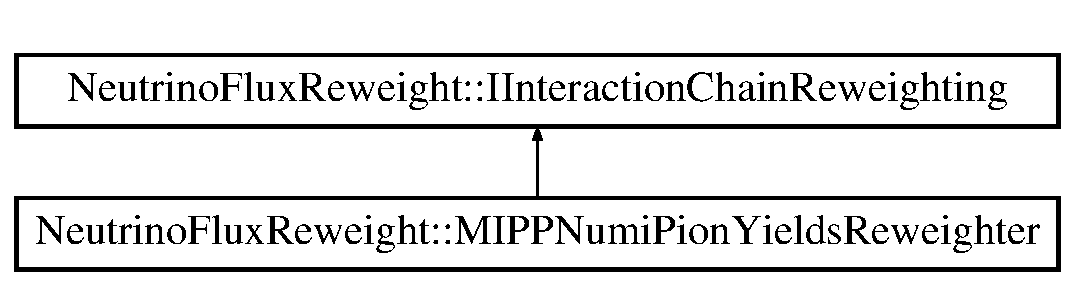
\includegraphics[height=2.000000cm]{class_neutrino_flux_reweight_1_1_m_i_p_p_numi_pion_yields_reweighter}
\end{center}
\end{figure}
\subsection*{Public Member Functions}
\begin{DoxyCompactItemize}
\item 
\hyperlink{class_neutrino_flux_reweight_1_1_m_i_p_p_numi_pion_yields_reweighter_a0936dda1619b4d977b07868216d67d16}{M\-I\-P\-P\-Numi\-Pion\-Yields\-Reweighter} (int iuniv, const \hyperlink{class_neutrino_flux_reweight_1_1_parameter_table}{Parameter\-Table} \&cv\-\_\-pars, const \hyperlink{class_neutrino_flux_reweight_1_1_parameter_table}{Parameter\-Table} \&univ\-\_\-pars)
\item 
virtual \hyperlink{class_neutrino_flux_reweight_1_1_m_i_p_p_numi_pion_yields_reweighter_a6779850f19e6cf219b2ea83eed20b223}{$\sim$\-M\-I\-P\-P\-Numi\-Pion\-Yields\-Reweighter} ()
\item 
virtual std\-::vector$<$ bool $>$ \hyperlink{class_neutrino_flux_reweight_1_1_m_i_p_p_numi_pion_yields_reweighter_a6a716b25ddb7d29ace9c7f07d84c91b2}{can\-Reweight} (const \hyperlink{class_neutrino_flux_reweight_1_1_interaction_chain_data}{Interaction\-Chain\-Data} \&aa)
\begin{DoxyCompactList}\small\item\em Look through the \hyperlink{class_neutrino_flux_reweight_1_1_interaction_chain_data}{Interaction\-Chain\-Data} input and identify those Interactions that can be reweighted as part of a chain. We return a vector indicating which elements will be assigned a weight by calculate\-Weight. \end{DoxyCompactList}\item 
virtual double \hyperlink{class_neutrino_flux_reweight_1_1_m_i_p_p_numi_pion_yields_reweighter_a84ef113a8ef34c2f9f5813938ec35382}{calculate\-Weight} (const \hyperlink{class_neutrino_flux_reweight_1_1_interaction_chain_data}{Interaction\-Chain\-Data} \&aa)
\begin{DoxyCompactList}\small\item\em calculate a weight for this interaction chain given the central value parameters and the parameters for this universe. The weight is something like\-: f(cv)/f(M\-C) $\ast$ f(univ)/f(cv) where cv in this case corresponds to the best value of the parameter, given the data. If univ\-\_\-pars=cv\-\_\-pars then we are calculating a central value weight. Note, \hyperlink{class_neutrino_flux_reweight_1_1_m_i_p_p_numi_pion_yields_reweighter_a6a716b25ddb7d29ace9c7f07d84c91b2}{can\-Reweight()} should be called to determine which elements of the chain are covered by the weight returned by \hyperlink{class_neutrino_flux_reweight_1_1_m_i_p_p_numi_pion_yields_reweighter_a84ef113a8ef34c2f9f5813938ec35382}{calculate\-Weight()} \end{DoxyCompactList}\end{DoxyCompactItemize}
\subsection*{Public Attributes}
\begin{DoxyCompactItemize}
\item 
const \hyperlink{class_neutrino_flux_reweight_1_1_parameter_table}{Parameter\-Table} \& \hyperlink{class_neutrino_flux_reweight_1_1_m_i_p_p_numi_pion_yields_reweighter_a127384f58575ad94c986aac85ea6fbe6}{cv\-Pars}
\item 
const \hyperlink{class_neutrino_flux_reweight_1_1_parameter_table}{Parameter\-Table} \& \hyperlink{class_neutrino_flux_reweight_1_1_m_i_p_p_numi_pion_yields_reweighter_a9208f5f3b7541f13f9e652d84e50c7cd}{univ\-Pars}
\end{DoxyCompactItemize}
\subsection*{Private Attributes}
\begin{DoxyCompactItemize}
\item 
int \hyperlink{class_neutrino_flux_reweight_1_1_m_i_p_p_numi_pion_yields_reweighter_a1ff57841eaa437aeb11a9793a64e47c2}{i\-Univ}
\item 
float \hyperlink{class_neutrino_flux_reweight_1_1_m_i_p_p_numi_pion_yields_reweighter_a90a2a88378549bb970b58543571206d7}{prt\-\_\-no\-\_\-inter}
\item 
std\-::vector$<$ float $>$ \hyperlink{class_neutrino_flux_reweight_1_1_m_i_p_p_numi_pion_yields_reweighter_a2120bbeea3e8b080eb68cd8ef6aa5b8e}{vbin\-\_\-data\-\_\-pip}
\item 
std\-::vector$<$ float $>$ \hyperlink{class_neutrino_flux_reweight_1_1_m_i_p_p_numi_pion_yields_reweighter_a812702b4afdcb56925d897e56a01b352}{vbin\-\_\-data\-\_\-pim}
\end{DoxyCompactItemize}


\subsection{Detailed Description}
Reweight a chain of interactions that are covered by the Nu\-M\-I target pi+ and pi-\/ yields measured by M\-I\-P\-P. 

Definition at line 12 of file M\-I\-P\-P\-Numi\-Pion\-Yields\-Reweighter.\-h.



\subsection{Constructor \& Destructor Documentation}
\hypertarget{class_neutrino_flux_reweight_1_1_m_i_p_p_numi_pion_yields_reweighter_a0936dda1619b4d977b07868216d67d16}{\index{Neutrino\-Flux\-Reweight\-::\-M\-I\-P\-P\-Numi\-Pion\-Yields\-Reweighter@{Neutrino\-Flux\-Reweight\-::\-M\-I\-P\-P\-Numi\-Pion\-Yields\-Reweighter}!M\-I\-P\-P\-Numi\-Pion\-Yields\-Reweighter@{M\-I\-P\-P\-Numi\-Pion\-Yields\-Reweighter}}
\index{M\-I\-P\-P\-Numi\-Pion\-Yields\-Reweighter@{M\-I\-P\-P\-Numi\-Pion\-Yields\-Reweighter}!NeutrinoFluxReweight::MIPPNumiPionYieldsReweighter@{Neutrino\-Flux\-Reweight\-::\-M\-I\-P\-P\-Numi\-Pion\-Yields\-Reweighter}}
\subsubsection[{M\-I\-P\-P\-Numi\-Pion\-Yields\-Reweighter}]{\setlength{\rightskip}{0pt plus 5cm}Neutrino\-Flux\-Reweight\-::\-M\-I\-P\-P\-Numi\-Pion\-Yields\-Reweighter\-::\-M\-I\-P\-P\-Numi\-Pion\-Yields\-Reweighter (
\begin{DoxyParamCaption}
\item[{int}]{iuniv, }
\item[{const {\bf Parameter\-Table} \&}]{cv\-\_\-pars, }
\item[{const {\bf Parameter\-Table} \&}]{univ\-\_\-pars}
\end{DoxyParamCaption}
)}}\label{class_neutrino_flux_reweight_1_1_m_i_p_p_numi_pion_yields_reweighter_a0936dda1619b4d977b07868216d67d16}
The constructor. Note, we pass central value and single universe parameters in this constructor only. There is thus a 1 to 1 correspondence between an instance of this class and a given universe. 

Definition at line 12 of file M\-I\-P\-P\-Numi\-Pion\-Yields\-Reweighter.\-cpp.


\begin{DoxyCode}
12                                                                                                            
                                :\hyperlink{class_neutrino_flux_reweight_1_1_m_i_p_p_numi_pion_yields_reweighter_a127384f58575ad94c986aac85ea6fbe6}{cvPars}(cv\_pars),\hyperlink{class_neutrino_flux_reweight_1_1_m_i_p_p_numi_pion_yields_reweighter_a9208f5f3b7541f13f9e652d84e50c7cd}{univPars}(univ\_pars),
      \hyperlink{class_neutrino_flux_reweight_1_1_m_i_p_p_numi_pion_yields_reweighter_a1ff57841eaa437aeb11a9793a64e47c2}{iUniv}(iuniv)\{ 
13 
14      MIPPNumiYieldsBins* MIPPbins =  \hyperlink{class_neutrino_flux_reweight_1_1_m_i_p_p_numi_yields_bins_a7f44afe90a846812d6eabfafa8f576e4}{MIPPNumiYieldsBins::getInstance}();
15      \hyperlink{class_neutrino_flux_reweight_1_1_m_i_p_p_numi_pion_yields_reweighter_a2120bbeea3e8b080eb68cd8ef6aa5b8e}{vbin\_data\_pip}.reserve(MIPPbins->GetNbins\_pip\_MIPPNuMI());
16      \hyperlink{class_neutrino_flux_reweight_1_1_m_i_p_p_numi_pion_yields_reweighter_a812702b4afdcb56925d897e56a01b352}{vbin\_data\_pim}.reserve(MIPPbins->GetNbins\_pim\_MIPPNuMI());
17      
18      \textcolor{comment}{//const boost::interprocess::flat\_map<std::string, double>& cv\_table = cvPars.getMap();}
19      \textcolor{comment}{//const boost::interprocess::flat\_map<std::string, double>& univ\_table = univPars.getMap();}
20     \hyperlink{class_neutrino_flux_reweight_1_1_m_i_p_p_numi_pion_yields_reweighter_a90a2a88378549bb970b58543571206d7}{prt\_no\_inter} = \hyperlink{class_neutrino_flux_reweight_1_1_m_i_p_p_numi_pion_yields_reweighter_a9208f5f3b7541f13f9e652d84e50c7cd}{univPars}.\hyperlink{class_neutrino_flux_reweight_1_1_parameter_table_acb7dc8335b65b116f6092f2fa57ca5ed}{getParameterValue}(\textcolor{stringliteral}{"prt\_no\_interacting"});
21     \textcolor{keywordtype}{char} namepar[100];
22     \textcolor{keywordflow}{for}(\textcolor{keywordtype}{int} ii=0;ii<MIPPbins->GetNbins\_pip\_MIPPNuMI();ii++)\{
23       sprintf(namepar,\textcolor{stringliteral}{"MIPP\_NuMI\_%s\_sys\_%d"},\textcolor{stringliteral}{"pip"},ii);
24       \textcolor{keywordtype}{double} data\_cv  = \hyperlink{class_neutrino_flux_reweight_1_1_m_i_p_p_numi_pion_yields_reweighter_a127384f58575ad94c986aac85ea6fbe6}{cvPars}.\hyperlink{class_neutrino_flux_reweight_1_1_parameter_table_acb7dc8335b65b116f6092f2fa57ca5ed}{getParameterValue}(std::string(namepar));
25       \textcolor{keywordtype}{double} data\_sys = \hyperlink{class_neutrino_flux_reweight_1_1_m_i_p_p_numi_pion_yields_reweighter_a9208f5f3b7541f13f9e652d84e50c7cd}{univPars}.\hyperlink{class_neutrino_flux_reweight_1_1_parameter_table_acb7dc8335b65b116f6092f2fa57ca5ed}{getParameterValue}(std::string(namepar));
26       sprintf(namepar,\textcolor{stringliteral}{"MIPP\_NuMI\_%s\_stats\_%d"},\textcolor{stringliteral}{"pip"},ii);
27       \textcolor{keywordtype}{double} data\_sta = \hyperlink{class_neutrino_flux_reweight_1_1_m_i_p_p_numi_pion_yields_reweighter_a9208f5f3b7541f13f9e652d84e50c7cd}{univPars}.\hyperlink{class_neutrino_flux_reweight_1_1_parameter_table_acb7dc8335b65b116f6092f2fa57ca5ed}{getParameterValue}(std::string(namepar));
28       data\_sys /= (1.0-\hyperlink{class_neutrino_flux_reweight_1_1_m_i_p_p_numi_pion_yields_reweighter_a90a2a88378549bb970b58543571206d7}{prt\_no\_inter});
29       data\_sta /= (1.0-\hyperlink{class_neutrino_flux_reweight_1_1_m_i_p_p_numi_pion_yields_reweighter_a90a2a88378549bb970b58543571206d7}{prt\_no\_inter});
30       data\_cv  /= (1.0-\hyperlink{class_neutrino_flux_reweight_1_1_m_i_p_p_numi_pion_yields_reweighter_a90a2a88378549bb970b58543571206d7}{prt\_no\_inter});
31       \hyperlink{class_neutrino_flux_reweight_1_1_m_i_p_p_numi_pion_yields_reweighter_a2120bbeea3e8b080eb68cd8ef6aa5b8e}{vbin\_data\_pip}.push\_back(data\_sys + data\_sta - data\_cv);
32     \}
33     \textcolor{keywordflow}{for}(\textcolor{keywordtype}{int} ii=0;ii<MIPPbins->GetNbins\_pim\_MIPPNuMI();ii++)\{
34       sprintf(namepar,\textcolor{stringliteral}{"MIPP\_NuMI\_%s\_sys\_%d"},\textcolor{stringliteral}{"pim"},ii);
35       \textcolor{keywordtype}{double} data\_cv  = \hyperlink{class_neutrino_flux_reweight_1_1_m_i_p_p_numi_pion_yields_reweighter_a127384f58575ad94c986aac85ea6fbe6}{cvPars}.\hyperlink{class_neutrino_flux_reweight_1_1_parameter_table_acb7dc8335b65b116f6092f2fa57ca5ed}{getParameterValue}(std::string(namepar));
36       \textcolor{keywordtype}{double} data\_sys = \hyperlink{class_neutrino_flux_reweight_1_1_m_i_p_p_numi_pion_yields_reweighter_a9208f5f3b7541f13f9e652d84e50c7cd}{univPars}.\hyperlink{class_neutrino_flux_reweight_1_1_parameter_table_acb7dc8335b65b116f6092f2fa57ca5ed}{getParameterValue}(std::string(namepar));
37       sprintf(namepar,\textcolor{stringliteral}{"MIPP\_NuMI\_%s\_stats\_%d"},\textcolor{stringliteral}{"pim"},ii);
38       \textcolor{keywordtype}{double} data\_sta = \hyperlink{class_neutrino_flux_reweight_1_1_m_i_p_p_numi_pion_yields_reweighter_a9208f5f3b7541f13f9e652d84e50c7cd}{univPars}.\hyperlink{class_neutrino_flux_reweight_1_1_parameter_table_acb7dc8335b65b116f6092f2fa57ca5ed}{getParameterValue}(std::string(namepar));
39       data\_sys /= (1.0-\hyperlink{class_neutrino_flux_reweight_1_1_m_i_p_p_numi_pion_yields_reweighter_a90a2a88378549bb970b58543571206d7}{prt\_no\_inter});
40       data\_sta /= (1.0-\hyperlink{class_neutrino_flux_reweight_1_1_m_i_p_p_numi_pion_yields_reweighter_a90a2a88378549bb970b58543571206d7}{prt\_no\_inter});
41       data\_cv  /= (1.0-\hyperlink{class_neutrino_flux_reweight_1_1_m_i_p_p_numi_pion_yields_reweighter_a90a2a88378549bb970b58543571206d7}{prt\_no\_inter});
42       \hyperlink{class_neutrino_flux_reweight_1_1_m_i_p_p_numi_pion_yields_reweighter_a812702b4afdcb56925d897e56a01b352}{vbin\_data\_pim}.push\_back(data\_sys + data\_sta - data\_cv);
43     \}
44 
45     
46 \}
\end{DoxyCode}
\hypertarget{class_neutrino_flux_reweight_1_1_m_i_p_p_numi_pion_yields_reweighter_a6779850f19e6cf219b2ea83eed20b223}{\index{Neutrino\-Flux\-Reweight\-::\-M\-I\-P\-P\-Numi\-Pion\-Yields\-Reweighter@{Neutrino\-Flux\-Reweight\-::\-M\-I\-P\-P\-Numi\-Pion\-Yields\-Reweighter}!$\sim$\-M\-I\-P\-P\-Numi\-Pion\-Yields\-Reweighter@{$\sim$\-M\-I\-P\-P\-Numi\-Pion\-Yields\-Reweighter}}
\index{$\sim$\-M\-I\-P\-P\-Numi\-Pion\-Yields\-Reweighter@{$\sim$\-M\-I\-P\-P\-Numi\-Pion\-Yields\-Reweighter}!NeutrinoFluxReweight::MIPPNumiPionYieldsReweighter@{Neutrino\-Flux\-Reweight\-::\-M\-I\-P\-P\-Numi\-Pion\-Yields\-Reweighter}}
\subsubsection[{$\sim$\-M\-I\-P\-P\-Numi\-Pion\-Yields\-Reweighter}]{\setlength{\rightskip}{0pt plus 5cm}Neutrino\-Flux\-Reweight\-::\-M\-I\-P\-P\-Numi\-Pion\-Yields\-Reweighter\-::$\sim$\-M\-I\-P\-P\-Numi\-Pion\-Yields\-Reweighter (
\begin{DoxyParamCaption}
{}
\end{DoxyParamCaption}
)\hspace{0.3cm}{\ttfamily [virtual]}}}\label{class_neutrino_flux_reweight_1_1_m_i_p_p_numi_pion_yields_reweighter_a6779850f19e6cf219b2ea83eed20b223}


Definition at line 47 of file M\-I\-P\-P\-Numi\-Pion\-Yields\-Reweighter.\-cpp.


\begin{DoxyCode}
47                                                              \{
48     
49   \}
\end{DoxyCode}


\subsection{Member Function Documentation}
\hypertarget{class_neutrino_flux_reweight_1_1_m_i_p_p_numi_pion_yields_reweighter_a84ef113a8ef34c2f9f5813938ec35382}{\index{Neutrino\-Flux\-Reweight\-::\-M\-I\-P\-P\-Numi\-Pion\-Yields\-Reweighter@{Neutrino\-Flux\-Reweight\-::\-M\-I\-P\-P\-Numi\-Pion\-Yields\-Reweighter}!calculate\-Weight@{calculate\-Weight}}
\index{calculate\-Weight@{calculate\-Weight}!NeutrinoFluxReweight::MIPPNumiPionYieldsReweighter@{Neutrino\-Flux\-Reweight\-::\-M\-I\-P\-P\-Numi\-Pion\-Yields\-Reweighter}}
\subsubsection[{calculate\-Weight}]{\setlength{\rightskip}{0pt plus 5cm}double Neutrino\-Flux\-Reweight\-::\-M\-I\-P\-P\-Numi\-Pion\-Yields\-Reweighter\-::calculate\-Weight (
\begin{DoxyParamCaption}
\item[{const {\bf Interaction\-Chain\-Data} \&}]{aa}
\end{DoxyParamCaption}
)\hspace{0.3cm}{\ttfamily [virtual]}}}\label{class_neutrino_flux_reweight_1_1_m_i_p_p_numi_pion_yields_reweighter_a84ef113a8ef34c2f9f5813938ec35382}


calculate a weight for this interaction chain given the central value parameters and the parameters for this universe. The weight is something like\-: f(cv)/f(M\-C) $\ast$ f(univ)/f(cv) where cv in this case corresponds to the best value of the parameter, given the data. If univ\-\_\-pars=cv\-\_\-pars then we are calculating a central value weight. Note, \hyperlink{class_neutrino_flux_reweight_1_1_m_i_p_p_numi_pion_yields_reweighter_a6a716b25ddb7d29ace9c7f07d84c91b2}{can\-Reweight()} should be called to determine which elements of the chain are covered by the weight returned by \hyperlink{class_neutrino_flux_reweight_1_1_m_i_p_p_numi_pion_yields_reweighter_a84ef113a8ef34c2f9f5813938ec35382}{calculate\-Weight()} 



Implements \hyperlink{class_neutrino_flux_reweight_1_1_i_interaction_chain_reweighting_ae28403553637013fdc720674ee24c7c5}{Neutrino\-Flux\-Reweight\-::\-I\-Interaction\-Chain\-Reweighting}.



Definition at line 86 of file M\-I\-P\-P\-Numi\-Pion\-Yields\-Reweighter.\-cpp.


\begin{DoxyCode}
86                                                                                     \{
87     
88     \textcolor{keywordtype}{double} wgt = 1.0;
89     
90     MIPPNumiYieldsBins*  MIPPbins =  \hyperlink{class_neutrino_flux_reweight_1_1_m_i_p_p_numi_yields_bins_a7f44afe90a846812d6eabfafa8f576e4}{MIPPNumiYieldsBins::getInstance}();
91     MIPPNumiMC*  MCval =  \hyperlink{class_neutrino_flux_reweight_1_1_m_i_p_p_numi_m_c_a4324da8640cc9a0d157d82e08da3a1c3}{MIPPNumiMC::getInstance}();    
92     
93     TargetData tar = aa.tar\_info;
94     \textcolor{keywordtype}{int} binID = MIPPbins->BinID(tar.Pz,tar.Pt,tar.Tar\_pdg);
95     
96     \textcolor{keywordflow}{if}(binID<0)\{
97       std::cout<<\textcolor{stringliteral}{"BINID ZERO:"} <<tar.Pz<<\textcolor{stringliteral}{" "}<<tar.Pt<<\textcolor{stringliteral}{" "} <<tar.Tar\_pdg<<std::endl;
98       \textcolor{keywordflow}{return} 1.0;
99     \}
100     
101     \textcolor{comment}{//Getting MC:}
102     \textcolor{keywordtype}{double} binC = MCval->getMCval(tar.Pz,tar.Pt,tar.Tar\_pdg);
103     \textcolor{keywordflow}{if}(binC<1.e-18)\{
104       std::cout<<\textcolor{stringliteral}{"LOW MC VAL: "}<<binC <<std::endl;
105       \textcolor{keywordflow}{return} 1.0;
106     \}
107     
108     \textcolor{keywordflow}{if}(tar.Tar\_pdg == 211)wgt = \hyperlink{class_neutrino_flux_reweight_1_1_m_i_p_p_numi_pion_yields_reweighter_a2120bbeea3e8b080eb68cd8ef6aa5b8e}{vbin\_data\_pip}[binID]/binC;
109     \textcolor{keywordflow}{if}(tar.Tar\_pdg ==-211)wgt = \hyperlink{class_neutrino_flux_reweight_1_1_m_i_p_p_numi_pion_yields_reweighter_a812702b4afdcb56925d897e56a01b352}{vbin\_data\_pim}[binID]/binC;
110     
111     \textcolor{keywordflow}{if}(wgt<0)std::cout<<\textcolor{stringliteral}{"TTMIPPPI check wgt(<0) "}<<\hyperlink{class_neutrino_flux_reweight_1_1_m_i_p_p_numi_pion_yields_reweighter_a1ff57841eaa437aeb11a9793a64e47c2}{iUniv}<<\textcolor{stringliteral}{" "}<<tar.Pz<<\textcolor{stringliteral}{" "}<<tar.Pt<<\textcolor{stringliteral}{" "}<<tar.Tar\_pdg<<
      std::endl;
112     \textcolor{keywordflow}{return} wgt;
113     
114   \}
\end{DoxyCode}
\hypertarget{class_neutrino_flux_reweight_1_1_m_i_p_p_numi_pion_yields_reweighter_a6a716b25ddb7d29ace9c7f07d84c91b2}{\index{Neutrino\-Flux\-Reweight\-::\-M\-I\-P\-P\-Numi\-Pion\-Yields\-Reweighter@{Neutrino\-Flux\-Reweight\-::\-M\-I\-P\-P\-Numi\-Pion\-Yields\-Reweighter}!can\-Reweight@{can\-Reweight}}
\index{can\-Reweight@{can\-Reweight}!NeutrinoFluxReweight::MIPPNumiPionYieldsReweighter@{Neutrino\-Flux\-Reweight\-::\-M\-I\-P\-P\-Numi\-Pion\-Yields\-Reweighter}}
\subsubsection[{can\-Reweight}]{\setlength{\rightskip}{0pt plus 5cm}std\-::vector$<$ bool $>$ Neutrino\-Flux\-Reweight\-::\-M\-I\-P\-P\-Numi\-Pion\-Yields\-Reweighter\-::can\-Reweight (
\begin{DoxyParamCaption}
\item[{const {\bf Interaction\-Chain\-Data} \&}]{aa}
\end{DoxyParamCaption}
)\hspace{0.3cm}{\ttfamily [virtual]}}}\label{class_neutrino_flux_reweight_1_1_m_i_p_p_numi_pion_yields_reweighter_a6a716b25ddb7d29ace9c7f07d84c91b2}


Look through the \hyperlink{class_neutrino_flux_reweight_1_1_interaction_chain_data}{Interaction\-Chain\-Data} input and identify those Interactions that can be reweighted as part of a chain. We return a vector indicating which elements will be assigned a weight by calculate\-Weight. 



Implements \hyperlink{class_neutrino_flux_reweight_1_1_i_interaction_chain_reweighting_aacf17580c1d316f0ebcdfdff7418e9e3}{Neutrino\-Flux\-Reweight\-::\-I\-Interaction\-Chain\-Reweighting}.



Definition at line 50 of file M\-I\-P\-P\-Numi\-Pion\-Yields\-Reweighter.\-cpp.


\begin{DoxyCode}
50                                                                                          \{
51  
52     MIPPNumiYieldsBins*  MIPPbins =  \hyperlink{class_neutrino_flux_reweight_1_1_m_i_p_p_numi_yields_bins_a7f44afe90a846812d6eabfafa8f576e4}{MIPPNumiYieldsBins::getInstance}();
53     std::vector<bool> this\_nodes;
54     \textcolor{keywordflow}{for}(\textcolor{keywordtype}{size\_t} ii=0;ii<(aa.interaction\_chain).size();ii++)\{
55       this\_nodes.push\_back(\textcolor{keyword}{false});
56     \}
57    
58     \textcolor{comment}{//Look for MIPP Numi events}
59     \textcolor{comment}{//if the code find a MIPP Numi event, it will look }
60     \textcolor{comment}{//for how many interaction nodes covers}
61     \textcolor{comment}{//if not, return all nodes false.}
62     \textcolor{comment}{//bool is\_there\_mipp = false;   }
63     TargetData tar = aa.tar\_info;
64     \textcolor{comment}{//Cheking if the particle is a pion plus and pion minus:}
65     \textcolor{keywordflow}{if}(tar.Tar\_pdg != 211 && tar.Tar\_pdg != -211)\textcolor{keywordflow}{return} this\_nodes;
66     \textcolor{keywordtype}{int} binID = MIPPbins->BinID(tar.Pz,tar.Pt,tar.Tar\_pdg);
67     \textcolor{keywordflow}{if}(binID<0) \textcolor{keywordflow}{return} this\_nodes;    
68     
69     \textcolor{comment}{//Now that we know that we have a MIPP Numi event, }
70     \textcolor{comment}{//we will see how many nodes are covered.}
71     std::vector<InteractionData> this\_interactions = aa.interaction\_chain; 
72     
73     \textcolor{comment}{//Now we have the index of the hadron that exit the target in the }
74     \textcolor{comment}{//ancesty chain:}
75     \textcolor{keywordflow}{if}(tar.Idx\_ancestry>=0)\{
76       \textcolor{keywordflow}{for}(\textcolor{keywordtype}{int} ii=0;ii<tar.Idx\_ancestry;ii++)\{
77         this\_nodes[ii] = \textcolor{keyword}{true};
78       \}
79     \}
80     \textcolor{keywordflow}{else}\{
81       \textcolor{comment}{//  std::cout<<"==>>SOMETHING WEIRD WITH MIPP NUMI "<<tar.Idx\_ancestry<<" "<<tar.Tar\_pdg<<std::endl;}
82     \}
83     
84     \textcolor{keywordflow}{return} this\_nodes;
85   \}
\end{DoxyCode}


\subsection{Member Data Documentation}
\hypertarget{class_neutrino_flux_reweight_1_1_m_i_p_p_numi_pion_yields_reweighter_a127384f58575ad94c986aac85ea6fbe6}{\index{Neutrino\-Flux\-Reweight\-::\-M\-I\-P\-P\-Numi\-Pion\-Yields\-Reweighter@{Neutrino\-Flux\-Reweight\-::\-M\-I\-P\-P\-Numi\-Pion\-Yields\-Reweighter}!cv\-Pars@{cv\-Pars}}
\index{cv\-Pars@{cv\-Pars}!NeutrinoFluxReweight::MIPPNumiPionYieldsReweighter@{Neutrino\-Flux\-Reweight\-::\-M\-I\-P\-P\-Numi\-Pion\-Yields\-Reweighter}}
\subsubsection[{cv\-Pars}]{\setlength{\rightskip}{0pt plus 5cm}const {\bf Parameter\-Table}\& Neutrino\-Flux\-Reweight\-::\-M\-I\-P\-P\-Numi\-Pion\-Yields\-Reweighter\-::cv\-Pars}}\label{class_neutrino_flux_reweight_1_1_m_i_p_p_numi_pion_yields_reweighter_a127384f58575ad94c986aac85ea6fbe6}


Definition at line 23 of file M\-I\-P\-P\-Numi\-Pion\-Yields\-Reweighter.\-h.

\hypertarget{class_neutrino_flux_reweight_1_1_m_i_p_p_numi_pion_yields_reweighter_a1ff57841eaa437aeb11a9793a64e47c2}{\index{Neutrino\-Flux\-Reweight\-::\-M\-I\-P\-P\-Numi\-Pion\-Yields\-Reweighter@{Neutrino\-Flux\-Reweight\-::\-M\-I\-P\-P\-Numi\-Pion\-Yields\-Reweighter}!i\-Univ@{i\-Univ}}
\index{i\-Univ@{i\-Univ}!NeutrinoFluxReweight::MIPPNumiPionYieldsReweighter@{Neutrino\-Flux\-Reweight\-::\-M\-I\-P\-P\-Numi\-Pion\-Yields\-Reweighter}}
\subsubsection[{i\-Univ}]{\setlength{\rightskip}{0pt plus 5cm}int Neutrino\-Flux\-Reweight\-::\-M\-I\-P\-P\-Numi\-Pion\-Yields\-Reweighter\-::i\-Univ\hspace{0.3cm}{\ttfamily [private]}}}\label{class_neutrino_flux_reweight_1_1_m_i_p_p_numi_pion_yields_reweighter_a1ff57841eaa437aeb11a9793a64e47c2}


Definition at line 27 of file M\-I\-P\-P\-Numi\-Pion\-Yields\-Reweighter.\-h.

\hypertarget{class_neutrino_flux_reweight_1_1_m_i_p_p_numi_pion_yields_reweighter_a90a2a88378549bb970b58543571206d7}{\index{Neutrino\-Flux\-Reweight\-::\-M\-I\-P\-P\-Numi\-Pion\-Yields\-Reweighter@{Neutrino\-Flux\-Reweight\-::\-M\-I\-P\-P\-Numi\-Pion\-Yields\-Reweighter}!prt\-\_\-no\-\_\-inter@{prt\-\_\-no\-\_\-inter}}
\index{prt\-\_\-no\-\_\-inter@{prt\-\_\-no\-\_\-inter}!NeutrinoFluxReweight::MIPPNumiPionYieldsReweighter@{Neutrino\-Flux\-Reweight\-::\-M\-I\-P\-P\-Numi\-Pion\-Yields\-Reweighter}}
\subsubsection[{prt\-\_\-no\-\_\-inter}]{\setlength{\rightskip}{0pt plus 5cm}float Neutrino\-Flux\-Reweight\-::\-M\-I\-P\-P\-Numi\-Pion\-Yields\-Reweighter\-::prt\-\_\-no\-\_\-inter\hspace{0.3cm}{\ttfamily [private]}}}\label{class_neutrino_flux_reweight_1_1_m_i_p_p_numi_pion_yields_reweighter_a90a2a88378549bb970b58543571206d7}


Definition at line 28 of file M\-I\-P\-P\-Numi\-Pion\-Yields\-Reweighter.\-h.

\hypertarget{class_neutrino_flux_reweight_1_1_m_i_p_p_numi_pion_yields_reweighter_a9208f5f3b7541f13f9e652d84e50c7cd}{\index{Neutrino\-Flux\-Reweight\-::\-M\-I\-P\-P\-Numi\-Pion\-Yields\-Reweighter@{Neutrino\-Flux\-Reweight\-::\-M\-I\-P\-P\-Numi\-Pion\-Yields\-Reweighter}!univ\-Pars@{univ\-Pars}}
\index{univ\-Pars@{univ\-Pars}!NeutrinoFluxReweight::MIPPNumiPionYieldsReweighter@{Neutrino\-Flux\-Reweight\-::\-M\-I\-P\-P\-Numi\-Pion\-Yields\-Reweighter}}
\subsubsection[{univ\-Pars}]{\setlength{\rightskip}{0pt plus 5cm}const {\bf Parameter\-Table}\& Neutrino\-Flux\-Reweight\-::\-M\-I\-P\-P\-Numi\-Pion\-Yields\-Reweighter\-::univ\-Pars}}\label{class_neutrino_flux_reweight_1_1_m_i_p_p_numi_pion_yields_reweighter_a9208f5f3b7541f13f9e652d84e50c7cd}


Definition at line 24 of file M\-I\-P\-P\-Numi\-Pion\-Yields\-Reweighter.\-h.

\hypertarget{class_neutrino_flux_reweight_1_1_m_i_p_p_numi_pion_yields_reweighter_a812702b4afdcb56925d897e56a01b352}{\index{Neutrino\-Flux\-Reweight\-::\-M\-I\-P\-P\-Numi\-Pion\-Yields\-Reweighter@{Neutrino\-Flux\-Reweight\-::\-M\-I\-P\-P\-Numi\-Pion\-Yields\-Reweighter}!vbin\-\_\-data\-\_\-pim@{vbin\-\_\-data\-\_\-pim}}
\index{vbin\-\_\-data\-\_\-pim@{vbin\-\_\-data\-\_\-pim}!NeutrinoFluxReweight::MIPPNumiPionYieldsReweighter@{Neutrino\-Flux\-Reweight\-::\-M\-I\-P\-P\-Numi\-Pion\-Yields\-Reweighter}}
\subsubsection[{vbin\-\_\-data\-\_\-pim}]{\setlength{\rightskip}{0pt plus 5cm}std\-::vector$<$float$>$ Neutrino\-Flux\-Reweight\-::\-M\-I\-P\-P\-Numi\-Pion\-Yields\-Reweighter\-::vbin\-\_\-data\-\_\-pim\hspace{0.3cm}{\ttfamily [private]}}}\label{class_neutrino_flux_reweight_1_1_m_i_p_p_numi_pion_yields_reweighter_a812702b4afdcb56925d897e56a01b352}


Definition at line 29 of file M\-I\-P\-P\-Numi\-Pion\-Yields\-Reweighter.\-h.

\hypertarget{class_neutrino_flux_reweight_1_1_m_i_p_p_numi_pion_yields_reweighter_a2120bbeea3e8b080eb68cd8ef6aa5b8e}{\index{Neutrino\-Flux\-Reweight\-::\-M\-I\-P\-P\-Numi\-Pion\-Yields\-Reweighter@{Neutrino\-Flux\-Reweight\-::\-M\-I\-P\-P\-Numi\-Pion\-Yields\-Reweighter}!vbin\-\_\-data\-\_\-pip@{vbin\-\_\-data\-\_\-pip}}
\index{vbin\-\_\-data\-\_\-pip@{vbin\-\_\-data\-\_\-pip}!NeutrinoFluxReweight::MIPPNumiPionYieldsReweighter@{Neutrino\-Flux\-Reweight\-::\-M\-I\-P\-P\-Numi\-Pion\-Yields\-Reweighter}}
\subsubsection[{vbin\-\_\-data\-\_\-pip}]{\setlength{\rightskip}{0pt plus 5cm}std\-::vector$<$float$>$ Neutrino\-Flux\-Reweight\-::\-M\-I\-P\-P\-Numi\-Pion\-Yields\-Reweighter\-::vbin\-\_\-data\-\_\-pip\hspace{0.3cm}{\ttfamily [private]}}}\label{class_neutrino_flux_reweight_1_1_m_i_p_p_numi_pion_yields_reweighter_a2120bbeea3e8b080eb68cd8ef6aa5b8e}


Definition at line 29 of file M\-I\-P\-P\-Numi\-Pion\-Yields\-Reweighter.\-h.



The documentation for this class was generated from the following files\-:\begin{DoxyCompactItemize}
\item 
include/\hyperlink{_m_i_p_p_numi_pion_yields_reweighter_8h}{M\-I\-P\-P\-Numi\-Pion\-Yields\-Reweighter.\-h}\item 
src/\hyperlink{_m_i_p_p_numi_pion_yields_reweighter_8cpp}{M\-I\-P\-P\-Numi\-Pion\-Yields\-Reweighter.\-cpp}\end{DoxyCompactItemize}

\hypertarget{class_neutrino_flux_reweight_1_1_m_i_p_p_numi_yields_bins}{\section{Neutrino\-Flux\-Reweight\-:\-:M\-I\-P\-P\-Numi\-Yields\-Bins Class Reference}
\label{class_neutrino_flux_reweight_1_1_m_i_p_p_numi_yields_bins}\index{Neutrino\-Flux\-Reweight\-::\-M\-I\-P\-P\-Numi\-Yields\-Bins@{Neutrino\-Flux\-Reweight\-::\-M\-I\-P\-P\-Numi\-Yields\-Bins}}
}


A class to manage the bin definitions for M\-I\-P\-P Numi Yields.  




{\ttfamily \#include $<$M\-I\-P\-P\-Numi\-Yields\-Bins.\-h$>$}

\subsection*{Public Member Functions}
\begin{DoxyCompactItemize}
\item 
void \hyperlink{class_neutrino_flux_reweight_1_1_m_i_p_p_numi_yields_bins_a05c50ba3849b67cd871c4f1613d53c1a}{pip\-\_\-data\-\_\-from\-\_\-xml} (const char $\ast$filename)
\begin{DoxyCompactList}\small\item\em Read a xml pip file name to parse the bins. \end{DoxyCompactList}\item 
void \hyperlink{class_neutrino_flux_reweight_1_1_m_i_p_p_numi_yields_bins_a4032ced2609fbf5babe8c2d10f8630cc}{pim\-\_\-data\-\_\-from\-\_\-xml} (const char $\ast$filename)
\begin{DoxyCompactList}\small\item\em Read a xml pim file name to parse the bins. \end{DoxyCompactList}\item 
void \hyperlink{class_neutrino_flux_reweight_1_1_m_i_p_p_numi_yields_bins_aad185432f167028162f33fe50b39c534}{k\-\_\-pi\-\_\-data\-\_\-from\-\_\-xml} (const char $\ast$filename)
\begin{DoxyCompactList}\small\item\em Read a xml kaons over pions file name to parse the bins. \end{DoxyCompactList}\item 
int \hyperlink{class_neutrino_flux_reweight_1_1_m_i_p_p_numi_yields_bins_a2353da8099269fa78294386dd5be23f4}{Bin\-I\-D} (double pz, double pt, int pdgcode)
\begin{DoxyCompactList}\small\item\em Return the Bin I\-D for this data. \end{DoxyCompactList}\item 
int \hyperlink{class_neutrino_flux_reweight_1_1_m_i_p_p_numi_yields_bins_aa33ade6e9d1af8fa36ab14429aee3f48}{Get\-Nbins\-\_\-pip\-\_\-\-M\-I\-P\-P\-Nu\-M\-I} ()
\item 
int \hyperlink{class_neutrino_flux_reweight_1_1_m_i_p_p_numi_yields_bins_a6a9993f90a6b4c9963076ec945577131}{Get\-Nbins\-\_\-pim\-\_\-\-M\-I\-P\-P\-Nu\-M\-I} ()
\item 
int \hyperlink{class_neutrino_flux_reweight_1_1_m_i_p_p_numi_yields_bins_a4aabd71b9d87441340360cf009546148}{Get\-Nbins\-\_\-\-K\-\_\-\-M\-I\-P\-P\-Nu\-M\-I} ()
\end{DoxyCompactItemize}
\subsection*{Static Public Member Functions}
\begin{DoxyCompactItemize}
\item 
static \hyperlink{class_neutrino_flux_reweight_1_1_m_i_p_p_numi_yields_bins}{M\-I\-P\-P\-Numi\-Yields\-Bins} $\ast$ \hyperlink{class_neutrino_flux_reweight_1_1_m_i_p_p_numi_yields_bins_a7f44afe90a846812d6eabfafa8f576e4}{get\-Instance} ()
\end{DoxyCompactItemize}
\subsection*{Public Attributes}
\begin{DoxyCompactItemize}
\item 
std\-::vector$<$ double $>$ \hyperlink{class_neutrino_flux_reweight_1_1_m_i_p_p_numi_yields_bins_aa9625cf6520d1906b084fc7051e28e64}{pip\-\_\-data\-\_\-pzmin}
\item 
std\-::vector$<$ double $>$ \hyperlink{class_neutrino_flux_reweight_1_1_m_i_p_p_numi_yields_bins_a9702c80785cd8eec150cf8a6091192a7}{pim\-\_\-data\-\_\-pzmin}
\item 
std\-::vector$<$ double $>$ \hyperlink{class_neutrino_flux_reweight_1_1_m_i_p_p_numi_yields_bins_a2184256a52d72a1674b7a7a595ad60c9}{k\-\_\-pi\-\_\-data\-\_\-pzmin}
\item 
std\-::vector$<$ double $>$ \hyperlink{class_neutrino_flux_reweight_1_1_m_i_p_p_numi_yields_bins_a245698dccfcff92bc4d1bf3458e2d809}{pip\-\_\-data\-\_\-pzmax}
\item 
std\-::vector$<$ double $>$ \hyperlink{class_neutrino_flux_reweight_1_1_m_i_p_p_numi_yields_bins_aad61319f28e08168c4eabf6507987e29}{pim\-\_\-data\-\_\-pzmax}
\item 
std\-::vector$<$ double $>$ \hyperlink{class_neutrino_flux_reweight_1_1_m_i_p_p_numi_yields_bins_a1832b84f72664c0088c5f8cff20bb041}{k\-\_\-pi\-\_\-data\-\_\-pzmax}
\item 
std\-::vector$<$ double $>$ \hyperlink{class_neutrino_flux_reweight_1_1_m_i_p_p_numi_yields_bins_aec5bdb4bcc7c894e34db336163e0bc13}{pip\-\_\-data\-\_\-ptmin}
\item 
std\-::vector$<$ double $>$ \hyperlink{class_neutrino_flux_reweight_1_1_m_i_p_p_numi_yields_bins_a65177fce103ec850b5804f0ac3d0f5c4}{pim\-\_\-data\-\_\-ptmin}
\item 
std\-::vector$<$ double $>$ \hyperlink{class_neutrino_flux_reweight_1_1_m_i_p_p_numi_yields_bins_a91fe79424c764ccccd3cc31ca91b8cd1}{k\-\_\-pi\-\_\-data\-\_\-ptmin}
\item 
std\-::vector$<$ double $>$ \hyperlink{class_neutrino_flux_reweight_1_1_m_i_p_p_numi_yields_bins_a00b588132209a2d82ffef318273d451a}{pip\-\_\-data\-\_\-ptmax}
\item 
std\-::vector$<$ double $>$ \hyperlink{class_neutrino_flux_reweight_1_1_m_i_p_p_numi_yields_bins_a60a1e09716ccaec014d9ec25689b98be}{pim\-\_\-data\-\_\-ptmax}
\item 
std\-::vector$<$ double $>$ \hyperlink{class_neutrino_flux_reweight_1_1_m_i_p_p_numi_yields_bins_a589ef2889679d14791b9542303fc1322}{k\-\_\-pi\-\_\-data\-\_\-ptmax}
\end{DoxyCompactItemize}
\subsection*{Private Member Functions}
\begin{DoxyCompactItemize}
\item 
\hyperlink{class_neutrino_flux_reweight_1_1_m_i_p_p_numi_yields_bins_aa8028d8987a4322571d0a0852957ad8e}{M\-I\-P\-P\-Numi\-Yields\-Bins} ()
\end{DoxyCompactItemize}
\subsection*{Static Private Attributes}
\begin{DoxyCompactItemize}
\item 
static \hyperlink{class_neutrino_flux_reweight_1_1_m_i_p_p_numi_yields_bins}{M\-I\-P\-P\-Numi\-Yields\-Bins} $\ast$ \hyperlink{class_neutrino_flux_reweight_1_1_m_i_p_p_numi_yields_bins_a8a1080c839321c71204457f99e9c91e0}{instance} = 0
\end{DoxyCompactItemize}


\subsection{Detailed Description}
A class to manage the bin definitions for M\-I\-P\-P Numi Yields. 

Definition at line 13 of file M\-I\-P\-P\-Numi\-Yields\-Bins.\-h.



\subsection{Constructor \& Destructor Documentation}
\hypertarget{class_neutrino_flux_reweight_1_1_m_i_p_p_numi_yields_bins_aa8028d8987a4322571d0a0852957ad8e}{\index{Neutrino\-Flux\-Reweight\-::\-M\-I\-P\-P\-Numi\-Yields\-Bins@{Neutrino\-Flux\-Reweight\-::\-M\-I\-P\-P\-Numi\-Yields\-Bins}!M\-I\-P\-P\-Numi\-Yields\-Bins@{M\-I\-P\-P\-Numi\-Yields\-Bins}}
\index{M\-I\-P\-P\-Numi\-Yields\-Bins@{M\-I\-P\-P\-Numi\-Yields\-Bins}!NeutrinoFluxReweight::MIPPNumiYieldsBins@{Neutrino\-Flux\-Reweight\-::\-M\-I\-P\-P\-Numi\-Yields\-Bins}}
\subsubsection[{M\-I\-P\-P\-Numi\-Yields\-Bins}]{\setlength{\rightskip}{0pt plus 5cm}Neutrino\-Flux\-Reweight\-::\-M\-I\-P\-P\-Numi\-Yields\-Bins\-::\-M\-I\-P\-P\-Numi\-Yields\-Bins (
\begin{DoxyParamCaption}
{}
\end{DoxyParamCaption}
)\hspace{0.3cm}{\ttfamily [private]}}}\label{class_neutrino_flux_reweight_1_1_m_i_p_p_numi_yields_bins_aa8028d8987a4322571d0a0852957ad8e}


Definition at line 15 of file M\-I\-P\-P\-Numi\-Yields\-Bins.\-cpp.


\begin{DoxyCode}
15                                         \{
16   \}
\end{DoxyCode}


\subsection{Member Function Documentation}
\hypertarget{class_neutrino_flux_reweight_1_1_m_i_p_p_numi_yields_bins_a2353da8099269fa78294386dd5be23f4}{\index{Neutrino\-Flux\-Reweight\-::\-M\-I\-P\-P\-Numi\-Yields\-Bins@{Neutrino\-Flux\-Reweight\-::\-M\-I\-P\-P\-Numi\-Yields\-Bins}!Bin\-I\-D@{Bin\-I\-D}}
\index{Bin\-I\-D@{Bin\-I\-D}!NeutrinoFluxReweight::MIPPNumiYieldsBins@{Neutrino\-Flux\-Reweight\-::\-M\-I\-P\-P\-Numi\-Yields\-Bins}}
\subsubsection[{Bin\-I\-D}]{\setlength{\rightskip}{0pt plus 5cm}int Neutrino\-Flux\-Reweight\-::\-M\-I\-P\-P\-Numi\-Yields\-Bins\-::\-Bin\-I\-D (
\begin{DoxyParamCaption}
\item[{double}]{pz, }
\item[{double}]{pt, }
\item[{int}]{pdgcode}
\end{DoxyParamCaption}
)}}\label{class_neutrino_flux_reweight_1_1_m_i_p_p_numi_yields_bins_a2353da8099269fa78294386dd5be23f4}


Return the Bin I\-D for this data. 



Definition at line 105 of file M\-I\-P\-P\-Numi\-Yields\-Bins.\-cpp.


\begin{DoxyCode}
105                                                                \{
106 
107     \textcolor{keywordtype}{int} ibinID = -1;
108     
109     \textcolor{keywordtype}{int} size = 0;
110     \textcolor{keywordflow}{if}(pdgcode==211)\{
111       size = \hyperlink{class_neutrino_flux_reweight_1_1_m_i_p_p_numi_yields_bins_aa9625cf6520d1906b084fc7051e28e64}{pip\_data\_pzmin}.size();
112       \textcolor{keywordflow}{for}(\textcolor{keywordtype}{int} ii=0;ii<size;++ii)\{
113         \textcolor{keywordflow}{if}(pz>\hyperlink{class_neutrino_flux_reweight_1_1_m_i_p_p_numi_yields_bins_aa9625cf6520d1906b084fc7051e28e64}{pip\_data\_pzmin}[ii] && pz<\hyperlink{class_neutrino_flux_reweight_1_1_m_i_p_p_numi_yields_bins_a245698dccfcff92bc4d1bf3458e2d809}{pip\_data\_pzmax}[ii] && pt>
      \hyperlink{class_neutrino_flux_reweight_1_1_m_i_p_p_numi_yields_bins_aec5bdb4bcc7c894e34db336163e0bc13}{pip\_data\_ptmin}[ii] && pt<\hyperlink{class_neutrino_flux_reweight_1_1_m_i_p_p_numi_yields_bins_a00b588132209a2d82ffef318273d451a}{pip\_data\_ptmax}[ii])\{
114           ibinID = ii;
115         \}
116       \}
117       
118     \}
119     \textcolor{keywordflow}{if}(pdgcode==-211)\{
120       size = \hyperlink{class_neutrino_flux_reweight_1_1_m_i_p_p_numi_yields_bins_a9702c80785cd8eec150cf8a6091192a7}{pim\_data\_pzmin}.size();
121       \textcolor{keywordflow}{for}(\textcolor{keywordtype}{int} ii=0;ii<size;++ii)\{
122         \textcolor{keywordflow}{if}(pz>\hyperlink{class_neutrino_flux_reweight_1_1_m_i_p_p_numi_yields_bins_a9702c80785cd8eec150cf8a6091192a7}{pim\_data\_pzmin}[ii] && pz<\hyperlink{class_neutrino_flux_reweight_1_1_m_i_p_p_numi_yields_bins_aad61319f28e08168c4eabf6507987e29}{pim\_data\_pzmax}[ii] && pt>
      \hyperlink{class_neutrino_flux_reweight_1_1_m_i_p_p_numi_yields_bins_a65177fce103ec850b5804f0ac3d0f5c4}{pim\_data\_ptmin}[ii] && pt<\hyperlink{class_neutrino_flux_reweight_1_1_m_i_p_p_numi_yields_bins_a60a1e09716ccaec014d9ec25689b98be}{pim\_data\_ptmax}[ii])\{
123           ibinID = ii;
124         \}
125       \}
126       
127     \}
128     \textcolor{keywordflow}{if}(pdgcode==321 || pdgcode==-321 || pdgcode==130 || pdgcode==310)\{
129       size = \hyperlink{class_neutrino_flux_reweight_1_1_m_i_p_p_numi_yields_bins_a2184256a52d72a1674b7a7a595ad60c9}{k\_pi\_data\_pzmin}.size();
130       \textcolor{keywordflow}{for}(\textcolor{keywordtype}{int} ii=0;ii<size;++ii)\{
131         \textcolor{keywordflow}{if}(pz>\hyperlink{class_neutrino_flux_reweight_1_1_m_i_p_p_numi_yields_bins_a2184256a52d72a1674b7a7a595ad60c9}{k\_pi\_data\_pzmin}[ii] && pz<\hyperlink{class_neutrino_flux_reweight_1_1_m_i_p_p_numi_yields_bins_a1832b84f72664c0088c5f8cff20bb041}{k\_pi\_data\_pzmax}[ii] && pt>
      \hyperlink{class_neutrino_flux_reweight_1_1_m_i_p_p_numi_yields_bins_a91fe79424c764ccccd3cc31ca91b8cd1}{k\_pi\_data\_ptmin}[ii] && pt<\hyperlink{class_neutrino_flux_reweight_1_1_m_i_p_p_numi_yields_bins_a589ef2889679d14791b9542303fc1322}{k\_pi\_data\_ptmax}[ii])\{
132           ibinID = ii;
133         \}
134       \}
135     \}
136     \textcolor{keywordflow}{return} ibinID;
137     
138   \}
\end{DoxyCode}
\hypertarget{class_neutrino_flux_reweight_1_1_m_i_p_p_numi_yields_bins_a7f44afe90a846812d6eabfafa8f576e4}{\index{Neutrino\-Flux\-Reweight\-::\-M\-I\-P\-P\-Numi\-Yields\-Bins@{Neutrino\-Flux\-Reweight\-::\-M\-I\-P\-P\-Numi\-Yields\-Bins}!get\-Instance@{get\-Instance}}
\index{get\-Instance@{get\-Instance}!NeutrinoFluxReweight::MIPPNumiYieldsBins@{Neutrino\-Flux\-Reweight\-::\-M\-I\-P\-P\-Numi\-Yields\-Bins}}
\subsubsection[{get\-Instance}]{\setlength{\rightskip}{0pt plus 5cm}{\bf M\-I\-P\-P\-Numi\-Yields\-Bins} $\ast$ Neutrino\-Flux\-Reweight\-::\-M\-I\-P\-P\-Numi\-Yields\-Bins\-::get\-Instance (
\begin{DoxyParamCaption}
{}
\end{DoxyParamCaption}
)\hspace{0.3cm}{\ttfamily [static]}}}\label{class_neutrino_flux_reweight_1_1_m_i_p_p_numi_yields_bins_a7f44afe90a846812d6eabfafa8f576e4}


Definition at line 153 of file M\-I\-P\-P\-Numi\-Yields\-Bins.\-cpp.


\begin{DoxyCode}
153                                                      \{
154     \textcolor{keywordflow}{if} (\hyperlink{class_neutrino_flux_reweight_1_1_m_i_p_p_numi_yields_bins_a8a1080c839321c71204457f99e9c91e0}{instance} == 0) \hyperlink{class_neutrino_flux_reweight_1_1_m_i_p_p_numi_yields_bins_a8a1080c839321c71204457f99e9c91e0}{instance} = \textcolor{keyword}{new} \hyperlink{class_neutrino_flux_reweight_1_1_m_i_p_p_numi_yields_bins_aa8028d8987a4322571d0a0852957ad8e}{MIPPNumiYieldsBins};
155     \textcolor{keywordflow}{return} \hyperlink{class_neutrino_flux_reweight_1_1_m_i_p_p_numi_yields_bins_a8a1080c839321c71204457f99e9c91e0}{instance};
156   \}
\end{DoxyCode}
\hypertarget{class_neutrino_flux_reweight_1_1_m_i_p_p_numi_yields_bins_a4aabd71b9d87441340360cf009546148}{\index{Neutrino\-Flux\-Reweight\-::\-M\-I\-P\-P\-Numi\-Yields\-Bins@{Neutrino\-Flux\-Reweight\-::\-M\-I\-P\-P\-Numi\-Yields\-Bins}!Get\-Nbins\-\_\-\-K\-\_\-\-M\-I\-P\-P\-Nu\-M\-I@{Get\-Nbins\-\_\-\-K\-\_\-\-M\-I\-P\-P\-Nu\-M\-I}}
\index{Get\-Nbins\-\_\-\-K\-\_\-\-M\-I\-P\-P\-Nu\-M\-I@{Get\-Nbins\-\_\-\-K\-\_\-\-M\-I\-P\-P\-Nu\-M\-I}!NeutrinoFluxReweight::MIPPNumiYieldsBins@{Neutrino\-Flux\-Reweight\-::\-M\-I\-P\-P\-Numi\-Yields\-Bins}}
\subsubsection[{Get\-Nbins\-\_\-\-K\-\_\-\-M\-I\-P\-P\-Nu\-M\-I}]{\setlength{\rightskip}{0pt plus 5cm}int Neutrino\-Flux\-Reweight\-::\-M\-I\-P\-P\-Numi\-Yields\-Bins\-::\-Get\-Nbins\-\_\-\-K\-\_\-\-M\-I\-P\-P\-Nu\-M\-I (
\begin{DoxyParamCaption}
{}
\end{DoxyParamCaption}
)}}\label{class_neutrino_flux_reweight_1_1_m_i_p_p_numi_yields_bins_a4aabd71b9d87441340360cf009546148}


Definition at line 148 of file M\-I\-P\-P\-Numi\-Yields\-Bins.\-cpp.


\begin{DoxyCode}
148                                              \{
149     \textcolor{keywordflow}{if}(\hyperlink{class_neutrino_flux_reweight_1_1_m_i_p_p_numi_yields_bins_a2184256a52d72a1674b7a7a595ad60c9}{k\_pi\_data\_pzmin}.size()==0)\textcolor{keywordflow}{throw} std::runtime\_error(\textcolor{stringliteral}{"MIPPNumiYieldsBins has not been
       initialized!!"});
150     \textcolor{keywordflow}{return} \hyperlink{class_neutrino_flux_reweight_1_1_m_i_p_p_numi_yields_bins_a2184256a52d72a1674b7a7a595ad60c9}{k\_pi\_data\_pzmin}.size();
151   \}
\end{DoxyCode}
\hypertarget{class_neutrino_flux_reweight_1_1_m_i_p_p_numi_yields_bins_a6a9993f90a6b4c9963076ec945577131}{\index{Neutrino\-Flux\-Reweight\-::\-M\-I\-P\-P\-Numi\-Yields\-Bins@{Neutrino\-Flux\-Reweight\-::\-M\-I\-P\-P\-Numi\-Yields\-Bins}!Get\-Nbins\-\_\-pim\-\_\-\-M\-I\-P\-P\-Nu\-M\-I@{Get\-Nbins\-\_\-pim\-\_\-\-M\-I\-P\-P\-Nu\-M\-I}}
\index{Get\-Nbins\-\_\-pim\-\_\-\-M\-I\-P\-P\-Nu\-M\-I@{Get\-Nbins\-\_\-pim\-\_\-\-M\-I\-P\-P\-Nu\-M\-I}!NeutrinoFluxReweight::MIPPNumiYieldsBins@{Neutrino\-Flux\-Reweight\-::\-M\-I\-P\-P\-Numi\-Yields\-Bins}}
\subsubsection[{Get\-Nbins\-\_\-pim\-\_\-\-M\-I\-P\-P\-Nu\-M\-I}]{\setlength{\rightskip}{0pt plus 5cm}int Neutrino\-Flux\-Reweight\-::\-M\-I\-P\-P\-Numi\-Yields\-Bins\-::\-Get\-Nbins\-\_\-pim\-\_\-\-M\-I\-P\-P\-Nu\-M\-I (
\begin{DoxyParamCaption}
{}
\end{DoxyParamCaption}
)}}\label{class_neutrino_flux_reweight_1_1_m_i_p_p_numi_yields_bins_a6a9993f90a6b4c9963076ec945577131}


Definition at line 144 of file M\-I\-P\-P\-Numi\-Yields\-Bins.\-cpp.


\begin{DoxyCode}
144                                                \{
145     \textcolor{keywordflow}{if}(\hyperlink{class_neutrino_flux_reweight_1_1_m_i_p_p_numi_yields_bins_aa9625cf6520d1906b084fc7051e28e64}{pip\_data\_pzmin}.size()==0)\textcolor{keywordflow}{throw} std::runtime\_error(\textcolor{stringliteral}{"MIPPNumiYieldsBins has not been
       initialized!!"});
146     \textcolor{keywordflow}{return} \hyperlink{class_neutrino_flux_reweight_1_1_m_i_p_p_numi_yields_bins_a9702c80785cd8eec150cf8a6091192a7}{pim\_data\_pzmin}.size();
147   \}
\end{DoxyCode}
\hypertarget{class_neutrino_flux_reweight_1_1_m_i_p_p_numi_yields_bins_aa33ade6e9d1af8fa36ab14429aee3f48}{\index{Neutrino\-Flux\-Reweight\-::\-M\-I\-P\-P\-Numi\-Yields\-Bins@{Neutrino\-Flux\-Reweight\-::\-M\-I\-P\-P\-Numi\-Yields\-Bins}!Get\-Nbins\-\_\-pip\-\_\-\-M\-I\-P\-P\-Nu\-M\-I@{Get\-Nbins\-\_\-pip\-\_\-\-M\-I\-P\-P\-Nu\-M\-I}}
\index{Get\-Nbins\-\_\-pip\-\_\-\-M\-I\-P\-P\-Nu\-M\-I@{Get\-Nbins\-\_\-pip\-\_\-\-M\-I\-P\-P\-Nu\-M\-I}!NeutrinoFluxReweight::MIPPNumiYieldsBins@{Neutrino\-Flux\-Reweight\-::\-M\-I\-P\-P\-Numi\-Yields\-Bins}}
\subsubsection[{Get\-Nbins\-\_\-pip\-\_\-\-M\-I\-P\-P\-Nu\-M\-I}]{\setlength{\rightskip}{0pt plus 5cm}int Neutrino\-Flux\-Reweight\-::\-M\-I\-P\-P\-Numi\-Yields\-Bins\-::\-Get\-Nbins\-\_\-pip\-\_\-\-M\-I\-P\-P\-Nu\-M\-I (
\begin{DoxyParamCaption}
{}
\end{DoxyParamCaption}
)}}\label{class_neutrino_flux_reweight_1_1_m_i_p_p_numi_yields_bins_aa33ade6e9d1af8fa36ab14429aee3f48}


Definition at line 140 of file M\-I\-P\-P\-Numi\-Yields\-Bins.\-cpp.


\begin{DoxyCode}
140                                                \{
141     \textcolor{keywordflow}{if}(\hyperlink{class_neutrino_flux_reweight_1_1_m_i_p_p_numi_yields_bins_aa9625cf6520d1906b084fc7051e28e64}{pip\_data\_pzmin}.size()==0)\textcolor{keywordflow}{throw} std::runtime\_error(\textcolor{stringliteral}{"MIPPNumiYieldsBins has not been
       initialized!!"});
142     \textcolor{keywordflow}{return} \hyperlink{class_neutrino_flux_reweight_1_1_m_i_p_p_numi_yields_bins_aa9625cf6520d1906b084fc7051e28e64}{pip\_data\_pzmin}.size();
143   \}
\end{DoxyCode}
\hypertarget{class_neutrino_flux_reweight_1_1_m_i_p_p_numi_yields_bins_aad185432f167028162f33fe50b39c534}{\index{Neutrino\-Flux\-Reweight\-::\-M\-I\-P\-P\-Numi\-Yields\-Bins@{Neutrino\-Flux\-Reweight\-::\-M\-I\-P\-P\-Numi\-Yields\-Bins}!k\-\_\-pi\-\_\-data\-\_\-from\-\_\-xml@{k\-\_\-pi\-\_\-data\-\_\-from\-\_\-xml}}
\index{k\-\_\-pi\-\_\-data\-\_\-from\-\_\-xml@{k\-\_\-pi\-\_\-data\-\_\-from\-\_\-xml}!NeutrinoFluxReweight::MIPPNumiYieldsBins@{Neutrino\-Flux\-Reweight\-::\-M\-I\-P\-P\-Numi\-Yields\-Bins}}
\subsubsection[{k\-\_\-pi\-\_\-data\-\_\-from\-\_\-xml}]{\setlength{\rightskip}{0pt plus 5cm}void Neutrino\-Flux\-Reweight\-::\-M\-I\-P\-P\-Numi\-Yields\-Bins\-::k\-\_\-pi\-\_\-data\-\_\-from\-\_\-xml (
\begin{DoxyParamCaption}
\item[{const char $\ast$}]{filename}
\end{DoxyParamCaption}
)}}\label{class_neutrino_flux_reweight_1_1_m_i_p_p_numi_yields_bins_aad185432f167028162f33fe50b39c534}


Read a xml kaons over pions file name to parse the bins. 



Definition at line 77 of file M\-I\-P\-P\-Numi\-Yields\-Bins.\-cpp.


\begin{DoxyCode}
77                                                                  \{
78     \textcolor{keyword}{using} boost::property\_tree::ptree;
79     ptree top;
80     
81     read\_xml(filename,top,2); 
82     
83     ptree& binsK\_PI = top.get\_child(\textcolor{stringliteral}{"bins.MIPP\_Numi\_k\_pi"});
84      
85     ptree::iterator it = binsK\_PI.begin();
86     \textcolor{comment}{//int idx=0;}
87     \textcolor{keywordtype}{double} aux\_pzmin,aux\_pzmax,aux\_ptmin,aux\_ptmax;
88 
89     \textcolor{keywordflow}{for}(; it!=binsK\_PI.end(); ++it)\{
90       std::string pz\_string=it->second.get<std::string>(\textcolor{stringliteral}{"pzrange"});
91       std::string pt\_string=it->second.get<std::string>(\textcolor{stringliteral}{"ptrange"});
92       
93       std::stringstream ss1(pz\_string);
94       std::stringstream ss2(pt\_string);
95       ss1 >> aux\_pzmin >> aux\_pzmax;
96       ss2 >> aux\_ptmin >> aux\_ptmax;
97    
98       \hyperlink{class_neutrino_flux_reweight_1_1_m_i_p_p_numi_yields_bins_a2184256a52d72a1674b7a7a595ad60c9}{k\_pi\_data\_pzmin}.push\_back(aux\_pzmin);
99       \hyperlink{class_neutrino_flux_reweight_1_1_m_i_p_p_numi_yields_bins_a1832b84f72664c0088c5f8cff20bb041}{k\_pi\_data\_pzmax}.push\_back(aux\_pzmax);
100       \hyperlink{class_neutrino_flux_reweight_1_1_m_i_p_p_numi_yields_bins_a91fe79424c764ccccd3cc31ca91b8cd1}{k\_pi\_data\_ptmin}.push\_back(aux\_ptmin);
101       \hyperlink{class_neutrino_flux_reweight_1_1_m_i_p_p_numi_yields_bins_a589ef2889679d14791b9542303fc1322}{k\_pi\_data\_ptmax}.push\_back(aux\_ptmax);
102     \}
103   \}
\end{DoxyCode}
\hypertarget{class_neutrino_flux_reweight_1_1_m_i_p_p_numi_yields_bins_a4032ced2609fbf5babe8c2d10f8630cc}{\index{Neutrino\-Flux\-Reweight\-::\-M\-I\-P\-P\-Numi\-Yields\-Bins@{Neutrino\-Flux\-Reweight\-::\-M\-I\-P\-P\-Numi\-Yields\-Bins}!pim\-\_\-data\-\_\-from\-\_\-xml@{pim\-\_\-data\-\_\-from\-\_\-xml}}
\index{pim\-\_\-data\-\_\-from\-\_\-xml@{pim\-\_\-data\-\_\-from\-\_\-xml}!NeutrinoFluxReweight::MIPPNumiYieldsBins@{Neutrino\-Flux\-Reweight\-::\-M\-I\-P\-P\-Numi\-Yields\-Bins}}
\subsubsection[{pim\-\_\-data\-\_\-from\-\_\-xml}]{\setlength{\rightskip}{0pt plus 5cm}void Neutrino\-Flux\-Reweight\-::\-M\-I\-P\-P\-Numi\-Yields\-Bins\-::pim\-\_\-data\-\_\-from\-\_\-xml (
\begin{DoxyParamCaption}
\item[{const char $\ast$}]{filename}
\end{DoxyParamCaption}
)}}\label{class_neutrino_flux_reweight_1_1_m_i_p_p_numi_yields_bins_a4032ced2609fbf5babe8c2d10f8630cc}


Read a xml pim file name to parse the bins. 



Definition at line 48 of file M\-I\-P\-P\-Numi\-Yields\-Bins.\-cpp.


\begin{DoxyCode}
48                                                                 \{
49     \textcolor{keyword}{using} boost::property\_tree::ptree;
50     ptree top;
51     
52     read\_xml(filename,top,2); \textcolor{comment}{// option 2 removes comment strings}
53     
54     ptree& binsPIM = top.get\_child(\textcolor{stringliteral}{"bins.MIPP\_Numi\_pim"});
55      
56     ptree::iterator it = binsPIM.begin();
57     \textcolor{keywordtype}{double} aux\_pzmin,aux\_pzmax,aux\_ptmin,aux\_ptmax;
58 
59     \textcolor{keywordflow}{for}(; it!=binsPIM.end(); ++it)\{
60       \textcolor{comment}{// it->first is the name}
61       \textcolor{comment}{// it->second is the child property tree}
62       std::string pz\_string=it->second.get<std::string>(\textcolor{stringliteral}{"pzrange"});
63       std::string pt\_string=it->second.get<std::string>(\textcolor{stringliteral}{"ptrange"});
64       
65       std::stringstream ss1(pz\_string);
66       std::stringstream ss2(pt\_string);
67       ss1 >> aux\_pzmin >> aux\_pzmax;
68       ss2 >> aux\_ptmin >> aux\_ptmax;
69    
70       \hyperlink{class_neutrino_flux_reweight_1_1_m_i_p_p_numi_yields_bins_a9702c80785cd8eec150cf8a6091192a7}{pim\_data\_pzmin}.push\_back(aux\_pzmin);
71       \hyperlink{class_neutrino_flux_reweight_1_1_m_i_p_p_numi_yields_bins_aad61319f28e08168c4eabf6507987e29}{pim\_data\_pzmax}.push\_back(aux\_pzmax);
72       \hyperlink{class_neutrino_flux_reweight_1_1_m_i_p_p_numi_yields_bins_a65177fce103ec850b5804f0ac3d0f5c4}{pim\_data\_ptmin}.push\_back(aux\_ptmin);
73       \hyperlink{class_neutrino_flux_reweight_1_1_m_i_p_p_numi_yields_bins_a60a1e09716ccaec014d9ec25689b98be}{pim\_data\_ptmax}.push\_back(aux\_ptmax);
74     \}
75   \}
\end{DoxyCode}
\hypertarget{class_neutrino_flux_reweight_1_1_m_i_p_p_numi_yields_bins_a05c50ba3849b67cd871c4f1613d53c1a}{\index{Neutrino\-Flux\-Reweight\-::\-M\-I\-P\-P\-Numi\-Yields\-Bins@{Neutrino\-Flux\-Reweight\-::\-M\-I\-P\-P\-Numi\-Yields\-Bins}!pip\-\_\-data\-\_\-from\-\_\-xml@{pip\-\_\-data\-\_\-from\-\_\-xml}}
\index{pip\-\_\-data\-\_\-from\-\_\-xml@{pip\-\_\-data\-\_\-from\-\_\-xml}!NeutrinoFluxReweight::MIPPNumiYieldsBins@{Neutrino\-Flux\-Reweight\-::\-M\-I\-P\-P\-Numi\-Yields\-Bins}}
\subsubsection[{pip\-\_\-data\-\_\-from\-\_\-xml}]{\setlength{\rightskip}{0pt plus 5cm}void Neutrino\-Flux\-Reweight\-::\-M\-I\-P\-P\-Numi\-Yields\-Bins\-::pip\-\_\-data\-\_\-from\-\_\-xml (
\begin{DoxyParamCaption}
\item[{const char $\ast$}]{filename}
\end{DoxyParamCaption}
)}}\label{class_neutrino_flux_reweight_1_1_m_i_p_p_numi_yields_bins_a05c50ba3849b67cd871c4f1613d53c1a}


Read a xml pip file name to parse the bins. 



Definition at line 18 of file M\-I\-P\-P\-Numi\-Yields\-Bins.\-cpp.


\begin{DoxyCode}
18                                                                 \{
19     \textcolor{keyword}{using} boost::property\_tree::ptree;
20     ptree top;
21     
22     read\_xml(filename,top,2); \textcolor{comment}{// option 2 removes comment strings}
23     
24     ptree& binsPIP = top.get\_child(\textcolor{stringliteral}{"bins.MIPP\_Numi\_pip"});
25      
26     ptree::iterator it = binsPIP.begin();
27     \textcolor{comment}{//int idx=0;}
28     \textcolor{keywordtype}{double} aux\_pzmin,aux\_pzmax,aux\_ptmin,aux\_ptmax;
29 
30     \textcolor{keywordflow}{for}(; it!=binsPIP.end(); ++it)\{
31       \textcolor{comment}{// it->first is the name}
32       \textcolor{comment}{// it->second is the child property tree}
33       std::string pz\_string=it->second.get<std::string>(\textcolor{stringliteral}{"pzrange"});
34       std::string pt\_string=it->second.get<std::string>(\textcolor{stringliteral}{"ptrange"});
35       
36       std::stringstream ss1(pz\_string);
37       std::stringstream ss2(pt\_string);
38       ss1 >> aux\_pzmin >> aux\_pzmax;
39       ss2 >> aux\_ptmin >> aux\_ptmax;
40    
41       \hyperlink{class_neutrino_flux_reweight_1_1_m_i_p_p_numi_yields_bins_aa9625cf6520d1906b084fc7051e28e64}{pip\_data\_pzmin}.push\_back(aux\_pzmin);
42       \hyperlink{class_neutrino_flux_reweight_1_1_m_i_p_p_numi_yields_bins_a245698dccfcff92bc4d1bf3458e2d809}{pip\_data\_pzmax}.push\_back(aux\_pzmax);
43       \hyperlink{class_neutrino_flux_reweight_1_1_m_i_p_p_numi_yields_bins_aec5bdb4bcc7c894e34db336163e0bc13}{pip\_data\_ptmin}.push\_back(aux\_ptmin);
44       \hyperlink{class_neutrino_flux_reweight_1_1_m_i_p_p_numi_yields_bins_a00b588132209a2d82ffef318273d451a}{pip\_data\_ptmax}.push\_back(aux\_ptmax);
45     \}
46   \}
\end{DoxyCode}


\subsection{Member Data Documentation}
\hypertarget{class_neutrino_flux_reweight_1_1_m_i_p_p_numi_yields_bins_a8a1080c839321c71204457f99e9c91e0}{\index{Neutrino\-Flux\-Reweight\-::\-M\-I\-P\-P\-Numi\-Yields\-Bins@{Neutrino\-Flux\-Reweight\-::\-M\-I\-P\-P\-Numi\-Yields\-Bins}!instance@{instance}}
\index{instance@{instance}!NeutrinoFluxReweight::MIPPNumiYieldsBins@{Neutrino\-Flux\-Reweight\-::\-M\-I\-P\-P\-Numi\-Yields\-Bins}}
\subsubsection[{instance}]{\setlength{\rightskip}{0pt plus 5cm}{\bf M\-I\-P\-P\-Numi\-Yields\-Bins} $\ast$ Neutrino\-Flux\-Reweight\-::\-M\-I\-P\-P\-Numi\-Yields\-Bins\-::instance = 0\hspace{0.3cm}{\ttfamily [static]}, {\ttfamily [private]}}}\label{class_neutrino_flux_reweight_1_1_m_i_p_p_numi_yields_bins_a8a1080c839321c71204457f99e9c91e0}


Definition at line 44 of file M\-I\-P\-P\-Numi\-Yields\-Bins.\-h.

\hypertarget{class_neutrino_flux_reweight_1_1_m_i_p_p_numi_yields_bins_a589ef2889679d14791b9542303fc1322}{\index{Neutrino\-Flux\-Reweight\-::\-M\-I\-P\-P\-Numi\-Yields\-Bins@{Neutrino\-Flux\-Reweight\-::\-M\-I\-P\-P\-Numi\-Yields\-Bins}!k\-\_\-pi\-\_\-data\-\_\-ptmax@{k\-\_\-pi\-\_\-data\-\_\-ptmax}}
\index{k\-\_\-pi\-\_\-data\-\_\-ptmax@{k\-\_\-pi\-\_\-data\-\_\-ptmax}!NeutrinoFluxReweight::MIPPNumiYieldsBins@{Neutrino\-Flux\-Reweight\-::\-M\-I\-P\-P\-Numi\-Yields\-Bins}}
\subsubsection[{k\-\_\-pi\-\_\-data\-\_\-ptmax}]{\setlength{\rightskip}{0pt plus 5cm}std\-::vector$<$double$>$ Neutrino\-Flux\-Reweight\-::\-M\-I\-P\-P\-Numi\-Yields\-Bins\-::k\-\_\-pi\-\_\-data\-\_\-ptmax}}\label{class_neutrino_flux_reweight_1_1_m_i_p_p_numi_yields_bins_a589ef2889679d14791b9542303fc1322}


Definition at line 36 of file M\-I\-P\-P\-Numi\-Yields\-Bins.\-h.

\hypertarget{class_neutrino_flux_reweight_1_1_m_i_p_p_numi_yields_bins_a91fe79424c764ccccd3cc31ca91b8cd1}{\index{Neutrino\-Flux\-Reweight\-::\-M\-I\-P\-P\-Numi\-Yields\-Bins@{Neutrino\-Flux\-Reweight\-::\-M\-I\-P\-P\-Numi\-Yields\-Bins}!k\-\_\-pi\-\_\-data\-\_\-ptmin@{k\-\_\-pi\-\_\-data\-\_\-ptmin}}
\index{k\-\_\-pi\-\_\-data\-\_\-ptmin@{k\-\_\-pi\-\_\-data\-\_\-ptmin}!NeutrinoFluxReweight::MIPPNumiYieldsBins@{Neutrino\-Flux\-Reweight\-::\-M\-I\-P\-P\-Numi\-Yields\-Bins}}
\subsubsection[{k\-\_\-pi\-\_\-data\-\_\-ptmin}]{\setlength{\rightskip}{0pt plus 5cm}std\-::vector$<$double$>$ Neutrino\-Flux\-Reweight\-::\-M\-I\-P\-P\-Numi\-Yields\-Bins\-::k\-\_\-pi\-\_\-data\-\_\-ptmin}}\label{class_neutrino_flux_reweight_1_1_m_i_p_p_numi_yields_bins_a91fe79424c764ccccd3cc31ca91b8cd1}


Definition at line 35 of file M\-I\-P\-P\-Numi\-Yields\-Bins.\-h.

\hypertarget{class_neutrino_flux_reweight_1_1_m_i_p_p_numi_yields_bins_a1832b84f72664c0088c5f8cff20bb041}{\index{Neutrino\-Flux\-Reweight\-::\-M\-I\-P\-P\-Numi\-Yields\-Bins@{Neutrino\-Flux\-Reweight\-::\-M\-I\-P\-P\-Numi\-Yields\-Bins}!k\-\_\-pi\-\_\-data\-\_\-pzmax@{k\-\_\-pi\-\_\-data\-\_\-pzmax}}
\index{k\-\_\-pi\-\_\-data\-\_\-pzmax@{k\-\_\-pi\-\_\-data\-\_\-pzmax}!NeutrinoFluxReweight::MIPPNumiYieldsBins@{Neutrino\-Flux\-Reweight\-::\-M\-I\-P\-P\-Numi\-Yields\-Bins}}
\subsubsection[{k\-\_\-pi\-\_\-data\-\_\-pzmax}]{\setlength{\rightskip}{0pt plus 5cm}std\-::vector$<$double$>$ Neutrino\-Flux\-Reweight\-::\-M\-I\-P\-P\-Numi\-Yields\-Bins\-::k\-\_\-pi\-\_\-data\-\_\-pzmax}}\label{class_neutrino_flux_reweight_1_1_m_i_p_p_numi_yields_bins_a1832b84f72664c0088c5f8cff20bb041}


Definition at line 34 of file M\-I\-P\-P\-Numi\-Yields\-Bins.\-h.

\hypertarget{class_neutrino_flux_reweight_1_1_m_i_p_p_numi_yields_bins_a2184256a52d72a1674b7a7a595ad60c9}{\index{Neutrino\-Flux\-Reweight\-::\-M\-I\-P\-P\-Numi\-Yields\-Bins@{Neutrino\-Flux\-Reweight\-::\-M\-I\-P\-P\-Numi\-Yields\-Bins}!k\-\_\-pi\-\_\-data\-\_\-pzmin@{k\-\_\-pi\-\_\-data\-\_\-pzmin}}
\index{k\-\_\-pi\-\_\-data\-\_\-pzmin@{k\-\_\-pi\-\_\-data\-\_\-pzmin}!NeutrinoFluxReweight::MIPPNumiYieldsBins@{Neutrino\-Flux\-Reweight\-::\-M\-I\-P\-P\-Numi\-Yields\-Bins}}
\subsubsection[{k\-\_\-pi\-\_\-data\-\_\-pzmin}]{\setlength{\rightskip}{0pt plus 5cm}std\-::vector$<$double$>$ Neutrino\-Flux\-Reweight\-::\-M\-I\-P\-P\-Numi\-Yields\-Bins\-::k\-\_\-pi\-\_\-data\-\_\-pzmin}}\label{class_neutrino_flux_reweight_1_1_m_i_p_p_numi_yields_bins_a2184256a52d72a1674b7a7a595ad60c9}


Definition at line 33 of file M\-I\-P\-P\-Numi\-Yields\-Bins.\-h.

\hypertarget{class_neutrino_flux_reweight_1_1_m_i_p_p_numi_yields_bins_a60a1e09716ccaec014d9ec25689b98be}{\index{Neutrino\-Flux\-Reweight\-::\-M\-I\-P\-P\-Numi\-Yields\-Bins@{Neutrino\-Flux\-Reweight\-::\-M\-I\-P\-P\-Numi\-Yields\-Bins}!pim\-\_\-data\-\_\-ptmax@{pim\-\_\-data\-\_\-ptmax}}
\index{pim\-\_\-data\-\_\-ptmax@{pim\-\_\-data\-\_\-ptmax}!NeutrinoFluxReweight::MIPPNumiYieldsBins@{Neutrino\-Flux\-Reweight\-::\-M\-I\-P\-P\-Numi\-Yields\-Bins}}
\subsubsection[{pim\-\_\-data\-\_\-ptmax}]{\setlength{\rightskip}{0pt plus 5cm}std\-::vector$<$double$>$ Neutrino\-Flux\-Reweight\-::\-M\-I\-P\-P\-Numi\-Yields\-Bins\-::pim\-\_\-data\-\_\-ptmax}}\label{class_neutrino_flux_reweight_1_1_m_i_p_p_numi_yields_bins_a60a1e09716ccaec014d9ec25689b98be}


Definition at line 36 of file M\-I\-P\-P\-Numi\-Yields\-Bins.\-h.

\hypertarget{class_neutrino_flux_reweight_1_1_m_i_p_p_numi_yields_bins_a65177fce103ec850b5804f0ac3d0f5c4}{\index{Neutrino\-Flux\-Reweight\-::\-M\-I\-P\-P\-Numi\-Yields\-Bins@{Neutrino\-Flux\-Reweight\-::\-M\-I\-P\-P\-Numi\-Yields\-Bins}!pim\-\_\-data\-\_\-ptmin@{pim\-\_\-data\-\_\-ptmin}}
\index{pim\-\_\-data\-\_\-ptmin@{pim\-\_\-data\-\_\-ptmin}!NeutrinoFluxReweight::MIPPNumiYieldsBins@{Neutrino\-Flux\-Reweight\-::\-M\-I\-P\-P\-Numi\-Yields\-Bins}}
\subsubsection[{pim\-\_\-data\-\_\-ptmin}]{\setlength{\rightskip}{0pt plus 5cm}std\-::vector$<$double$>$ Neutrino\-Flux\-Reweight\-::\-M\-I\-P\-P\-Numi\-Yields\-Bins\-::pim\-\_\-data\-\_\-ptmin}}\label{class_neutrino_flux_reweight_1_1_m_i_p_p_numi_yields_bins_a65177fce103ec850b5804f0ac3d0f5c4}


Definition at line 35 of file M\-I\-P\-P\-Numi\-Yields\-Bins.\-h.

\hypertarget{class_neutrino_flux_reweight_1_1_m_i_p_p_numi_yields_bins_aad61319f28e08168c4eabf6507987e29}{\index{Neutrino\-Flux\-Reweight\-::\-M\-I\-P\-P\-Numi\-Yields\-Bins@{Neutrino\-Flux\-Reweight\-::\-M\-I\-P\-P\-Numi\-Yields\-Bins}!pim\-\_\-data\-\_\-pzmax@{pim\-\_\-data\-\_\-pzmax}}
\index{pim\-\_\-data\-\_\-pzmax@{pim\-\_\-data\-\_\-pzmax}!NeutrinoFluxReweight::MIPPNumiYieldsBins@{Neutrino\-Flux\-Reweight\-::\-M\-I\-P\-P\-Numi\-Yields\-Bins}}
\subsubsection[{pim\-\_\-data\-\_\-pzmax}]{\setlength{\rightskip}{0pt plus 5cm}std\-::vector$<$double$>$ Neutrino\-Flux\-Reweight\-::\-M\-I\-P\-P\-Numi\-Yields\-Bins\-::pim\-\_\-data\-\_\-pzmax}}\label{class_neutrino_flux_reweight_1_1_m_i_p_p_numi_yields_bins_aad61319f28e08168c4eabf6507987e29}


Definition at line 34 of file M\-I\-P\-P\-Numi\-Yields\-Bins.\-h.

\hypertarget{class_neutrino_flux_reweight_1_1_m_i_p_p_numi_yields_bins_a9702c80785cd8eec150cf8a6091192a7}{\index{Neutrino\-Flux\-Reweight\-::\-M\-I\-P\-P\-Numi\-Yields\-Bins@{Neutrino\-Flux\-Reweight\-::\-M\-I\-P\-P\-Numi\-Yields\-Bins}!pim\-\_\-data\-\_\-pzmin@{pim\-\_\-data\-\_\-pzmin}}
\index{pim\-\_\-data\-\_\-pzmin@{pim\-\_\-data\-\_\-pzmin}!NeutrinoFluxReweight::MIPPNumiYieldsBins@{Neutrino\-Flux\-Reweight\-::\-M\-I\-P\-P\-Numi\-Yields\-Bins}}
\subsubsection[{pim\-\_\-data\-\_\-pzmin}]{\setlength{\rightskip}{0pt plus 5cm}std\-::vector$<$double$>$ Neutrino\-Flux\-Reweight\-::\-M\-I\-P\-P\-Numi\-Yields\-Bins\-::pim\-\_\-data\-\_\-pzmin}}\label{class_neutrino_flux_reweight_1_1_m_i_p_p_numi_yields_bins_a9702c80785cd8eec150cf8a6091192a7}


Definition at line 33 of file M\-I\-P\-P\-Numi\-Yields\-Bins.\-h.

\hypertarget{class_neutrino_flux_reweight_1_1_m_i_p_p_numi_yields_bins_a00b588132209a2d82ffef318273d451a}{\index{Neutrino\-Flux\-Reweight\-::\-M\-I\-P\-P\-Numi\-Yields\-Bins@{Neutrino\-Flux\-Reweight\-::\-M\-I\-P\-P\-Numi\-Yields\-Bins}!pip\-\_\-data\-\_\-ptmax@{pip\-\_\-data\-\_\-ptmax}}
\index{pip\-\_\-data\-\_\-ptmax@{pip\-\_\-data\-\_\-ptmax}!NeutrinoFluxReweight::MIPPNumiYieldsBins@{Neutrino\-Flux\-Reweight\-::\-M\-I\-P\-P\-Numi\-Yields\-Bins}}
\subsubsection[{pip\-\_\-data\-\_\-ptmax}]{\setlength{\rightskip}{0pt plus 5cm}std\-::vector$<$double$>$ Neutrino\-Flux\-Reweight\-::\-M\-I\-P\-P\-Numi\-Yields\-Bins\-::pip\-\_\-data\-\_\-ptmax}}\label{class_neutrino_flux_reweight_1_1_m_i_p_p_numi_yields_bins_a00b588132209a2d82ffef318273d451a}


Definition at line 36 of file M\-I\-P\-P\-Numi\-Yields\-Bins.\-h.

\hypertarget{class_neutrino_flux_reweight_1_1_m_i_p_p_numi_yields_bins_aec5bdb4bcc7c894e34db336163e0bc13}{\index{Neutrino\-Flux\-Reweight\-::\-M\-I\-P\-P\-Numi\-Yields\-Bins@{Neutrino\-Flux\-Reweight\-::\-M\-I\-P\-P\-Numi\-Yields\-Bins}!pip\-\_\-data\-\_\-ptmin@{pip\-\_\-data\-\_\-ptmin}}
\index{pip\-\_\-data\-\_\-ptmin@{pip\-\_\-data\-\_\-ptmin}!NeutrinoFluxReweight::MIPPNumiYieldsBins@{Neutrino\-Flux\-Reweight\-::\-M\-I\-P\-P\-Numi\-Yields\-Bins}}
\subsubsection[{pip\-\_\-data\-\_\-ptmin}]{\setlength{\rightskip}{0pt plus 5cm}std\-::vector$<$double$>$ Neutrino\-Flux\-Reweight\-::\-M\-I\-P\-P\-Numi\-Yields\-Bins\-::pip\-\_\-data\-\_\-ptmin}}\label{class_neutrino_flux_reweight_1_1_m_i_p_p_numi_yields_bins_aec5bdb4bcc7c894e34db336163e0bc13}


Definition at line 35 of file M\-I\-P\-P\-Numi\-Yields\-Bins.\-h.

\hypertarget{class_neutrino_flux_reweight_1_1_m_i_p_p_numi_yields_bins_a245698dccfcff92bc4d1bf3458e2d809}{\index{Neutrino\-Flux\-Reweight\-::\-M\-I\-P\-P\-Numi\-Yields\-Bins@{Neutrino\-Flux\-Reweight\-::\-M\-I\-P\-P\-Numi\-Yields\-Bins}!pip\-\_\-data\-\_\-pzmax@{pip\-\_\-data\-\_\-pzmax}}
\index{pip\-\_\-data\-\_\-pzmax@{pip\-\_\-data\-\_\-pzmax}!NeutrinoFluxReweight::MIPPNumiYieldsBins@{Neutrino\-Flux\-Reweight\-::\-M\-I\-P\-P\-Numi\-Yields\-Bins}}
\subsubsection[{pip\-\_\-data\-\_\-pzmax}]{\setlength{\rightskip}{0pt plus 5cm}std\-::vector$<$double$>$ Neutrino\-Flux\-Reweight\-::\-M\-I\-P\-P\-Numi\-Yields\-Bins\-::pip\-\_\-data\-\_\-pzmax}}\label{class_neutrino_flux_reweight_1_1_m_i_p_p_numi_yields_bins_a245698dccfcff92bc4d1bf3458e2d809}


Definition at line 34 of file M\-I\-P\-P\-Numi\-Yields\-Bins.\-h.

\hypertarget{class_neutrino_flux_reweight_1_1_m_i_p_p_numi_yields_bins_aa9625cf6520d1906b084fc7051e28e64}{\index{Neutrino\-Flux\-Reweight\-::\-M\-I\-P\-P\-Numi\-Yields\-Bins@{Neutrino\-Flux\-Reweight\-::\-M\-I\-P\-P\-Numi\-Yields\-Bins}!pip\-\_\-data\-\_\-pzmin@{pip\-\_\-data\-\_\-pzmin}}
\index{pip\-\_\-data\-\_\-pzmin@{pip\-\_\-data\-\_\-pzmin}!NeutrinoFluxReweight::MIPPNumiYieldsBins@{Neutrino\-Flux\-Reweight\-::\-M\-I\-P\-P\-Numi\-Yields\-Bins}}
\subsubsection[{pip\-\_\-data\-\_\-pzmin}]{\setlength{\rightskip}{0pt plus 5cm}std\-::vector$<$double$>$ Neutrino\-Flux\-Reweight\-::\-M\-I\-P\-P\-Numi\-Yields\-Bins\-::pip\-\_\-data\-\_\-pzmin}}\label{class_neutrino_flux_reweight_1_1_m_i_p_p_numi_yields_bins_aa9625cf6520d1906b084fc7051e28e64}


Definition at line 33 of file M\-I\-P\-P\-Numi\-Yields\-Bins.\-h.



The documentation for this class was generated from the following files\-:\begin{DoxyCompactItemize}
\item 
include/\hyperlink{_m_i_p_p_numi_yields_bins_8h}{M\-I\-P\-P\-Numi\-Yields\-Bins.\-h}\item 
src/\hyperlink{_m_i_p_p_numi_yields_bins_8cpp}{M\-I\-P\-P\-Numi\-Yields\-Bins.\-cpp}\end{DoxyCompactItemize}

\hypertarget{struct_no_parameter_found}{\section{No\-Parameter\-Found Struct Reference}
\label{struct_no_parameter_found}\index{No\-Parameter\-Found@{No\-Parameter\-Found}}
}


{\ttfamily \#include $<$Exceptions.\-h$>$}

Inheritance diagram for No\-Parameter\-Found\-:\begin{figure}[H]
\begin{center}
\leavevmode
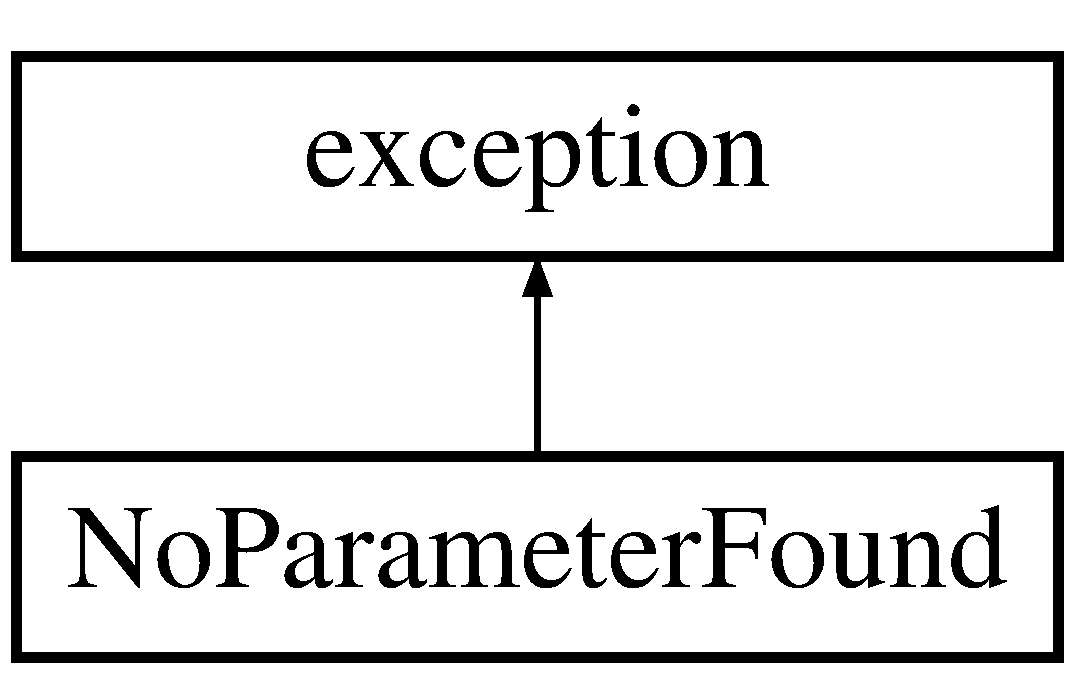
\includegraphics[height=2.000000cm]{struct_no_parameter_found}
\end{center}
\end{figure}
\subsection*{Public Member Functions}
\begin{DoxyCompactItemize}
\item 
\hyperlink{struct_no_parameter_found_ae0928e96c064f6cab3c88b5eb7263202}{No\-Parameter\-Found} (const std\-::string \&name)
\item 
virtual \hyperlink{struct_no_parameter_found_a9b8117cfa44fbf9ea15f42cfa1041d36}{$\sim$\-No\-Parameter\-Found} ()  throw ()
\item 
virtual const char $\ast$ \hyperlink{struct_no_parameter_found_ae7407095e9073afb09d7749c6b55b2e9}{what} () const   throw ()
\end{DoxyCompactItemize}
\subsection*{Public Attributes}
\begin{DoxyCompactItemize}
\item 
std\-::string \hyperlink{struct_no_parameter_found_a548745eb39b10918acd8199f21d7d455}{m\-\_\-error}
\end{DoxyCompactItemize}


\subsection{Detailed Description}


Definition at line 8 of file Exceptions.\-h.



\subsection{Constructor \& Destructor Documentation}
\hypertarget{struct_no_parameter_found_ae0928e96c064f6cab3c88b5eb7263202}{\index{No\-Parameter\-Found@{No\-Parameter\-Found}!No\-Parameter\-Found@{No\-Parameter\-Found}}
\index{No\-Parameter\-Found@{No\-Parameter\-Found}!NoParameterFound@{No\-Parameter\-Found}}
\subsubsection[{No\-Parameter\-Found}]{\setlength{\rightskip}{0pt plus 5cm}No\-Parameter\-Found\-::\-No\-Parameter\-Found (
\begin{DoxyParamCaption}
\item[{const std\-::string \&}]{name}
\end{DoxyParamCaption}
)\hspace{0.3cm}{\ttfamily [inline]}}}\label{struct_no_parameter_found_ae0928e96c064f6cab3c88b5eb7263202}


Definition at line 10 of file Exceptions.\-h.


\begin{DoxyCode}
11   \{
12     \hyperlink{struct_no_parameter_found_a548745eb39b10918acd8199f21d7d455}{m\_error}=std::string(\textcolor{stringliteral}{"Parameter not defined: "})+name;
13   \}
\end{DoxyCode}
\hypertarget{struct_no_parameter_found_a9b8117cfa44fbf9ea15f42cfa1041d36}{\index{No\-Parameter\-Found@{No\-Parameter\-Found}!$\sim$\-No\-Parameter\-Found@{$\sim$\-No\-Parameter\-Found}}
\index{$\sim$\-No\-Parameter\-Found@{$\sim$\-No\-Parameter\-Found}!NoParameterFound@{No\-Parameter\-Found}}
\subsubsection[{$\sim$\-No\-Parameter\-Found}]{\setlength{\rightskip}{0pt plus 5cm}virtual No\-Parameter\-Found\-::$\sim$\-No\-Parameter\-Found (
\begin{DoxyParamCaption}
{}
\end{DoxyParamCaption}
) throw  ) \hspace{0.3cm}{\ttfamily [inline]}, {\ttfamily [virtual]}}}\label{struct_no_parameter_found_a9b8117cfa44fbf9ea15f42cfa1041d36}


Definition at line 15 of file Exceptions.\-h.


\begin{DoxyCode}
15 \{\}
\end{DoxyCode}


\subsection{Member Function Documentation}
\hypertarget{struct_no_parameter_found_ae7407095e9073afb09d7749c6b55b2e9}{\index{No\-Parameter\-Found@{No\-Parameter\-Found}!what@{what}}
\index{what@{what}!NoParameterFound@{No\-Parameter\-Found}}
\subsubsection[{what}]{\setlength{\rightskip}{0pt plus 5cm}virtual const char$\ast$ No\-Parameter\-Found\-::what (
\begin{DoxyParamCaption}
{}
\end{DoxyParamCaption}
) const throw  ) \hspace{0.3cm}{\ttfamily [inline]}, {\ttfamily [virtual]}}}\label{struct_no_parameter_found_ae7407095e9073afb09d7749c6b55b2e9}


Definition at line 17 of file Exceptions.\-h.


\begin{DoxyCode}
17                                           \{
18     \textcolor{keywordflow}{return} \hyperlink{struct_no_parameter_found_a548745eb39b10918acd8199f21d7d455}{m\_error}.c\_str();
19   \}
\end{DoxyCode}


\subsection{Member Data Documentation}
\hypertarget{struct_no_parameter_found_a548745eb39b10918acd8199f21d7d455}{\index{No\-Parameter\-Found@{No\-Parameter\-Found}!m\-\_\-error@{m\-\_\-error}}
\index{m\-\_\-error@{m\-\_\-error}!NoParameterFound@{No\-Parameter\-Found}}
\subsubsection[{m\-\_\-error}]{\setlength{\rightskip}{0pt plus 5cm}std\-::string No\-Parameter\-Found\-::m\-\_\-error}}\label{struct_no_parameter_found_a548745eb39b10918acd8199f21d7d455}


Definition at line 21 of file Exceptions.\-h.



The documentation for this struct was generated from the following file\-:\begin{DoxyCompactItemize}
\item 
include/\hyperlink{_exceptions_8h}{Exceptions.\-h}\end{DoxyCompactItemize}

\hypertarget{classnu__g4numi}{\section{nu\-\_\-g4numi Class Reference}
\label{classnu__g4numi}\index{nu\-\_\-g4numi@{nu\-\_\-g4numi}}
}


{\ttfamily \#include $<$nu\-\_\-g4numi.\-h$>$}

\subsection*{Public Member Functions}
\begin{DoxyCompactItemize}
\item 
\hyperlink{classnu__g4numi_a5b94600aee440a46d7e7b4010d245a45}{nu\-\_\-g4numi} (T\-Chain $\ast$chain)
\item 
virtual \hyperlink{classnu__g4numi_a185e321ffe9aaf70d66490d2d2abfb37}{$\sim$nu\-\_\-g4numi} ()
\item 
void \hyperlink{classnu__g4numi_ad25cb6d8c5a184c1a626d26f944ef562}{Get\-Entry} (Int\-\_\-t ientry)
\end{DoxyCompactItemize}
\subsection*{Public Attributes}
\begin{DoxyCompactItemize}
\item 
Int\-\_\-t \hyperlink{classnu__g4numi_ab5167a93f34490c99c127d6f5292efb0}{Ntype}
\item 
Double\-\_\-t \hyperlink{classnu__g4numi_a36acd180b72c4686f55974e6783778ad}{Nenergy\-N} \mbox{[}11\mbox{]}
\item 
Double\-\_\-t \hyperlink{classnu__g4numi_a87ebc26325bb08a63d21171db959101a}{N\-Wt\-Near} \mbox{[}11\mbox{]}
\item 
Double\-\_\-t \hyperlink{classnu__g4numi_a47a88316abc9d5c30ba0c98893a441a8}{Nenergy\-F} \mbox{[}2\mbox{]}
\item 
Double\-\_\-t \hyperlink{classnu__g4numi_ab097def1361df4a718707a7e757bb2ae}{N\-Wt\-Far} \mbox{[}2\mbox{]}
\item 
Double\-\_\-t \hyperlink{classnu__g4numi_ae9ebb4d9a2b72dd69f17143ce6e41da0}{Nimpwt}
\item 
Int\-\_\-t \hyperlink{classnu__g4numi_abdbe76af4b20f3b5b5b2fb4b92156b42}{ntrajectory}
\item 
Bool\-\_\-t \hyperlink{classnu__g4numi_ad584f37592af684c65205de115a9aa85}{overflow}
\item 
Int\-\_\-t \hyperlink{classnu__g4numi_a4ed6688aee6debd26637a0401e5ef475}{pdg} \mbox{[}10\mbox{]}
\item 
Double\-\_\-t \hyperlink{classnu__g4numi_a309ea4b88683c5978593c0d474b1a976}{startpx} \mbox{[}10\mbox{]}
\item 
Double\-\_\-t \hyperlink{classnu__g4numi_a5247e8e73a100a7064f032806f542d38}{startpy} \mbox{[}10\mbox{]}
\item 
Double\-\_\-t \hyperlink{classnu__g4numi_a6bec79e4a2effa3cdaa28a1f02ae8124}{startpz} \mbox{[}10\mbox{]}
\item 
Double\-\_\-t \hyperlink{classnu__g4numi_a54b6004629ee3afa4f5e06b258def720}{stoppx} \mbox{[}10\mbox{]}
\item 
Double\-\_\-t \hyperlink{classnu__g4numi_a74c6c24c0fcad6777bedb8ba6a0e3787}{stoppy} \mbox{[}10\mbox{]}
\item 
Double\-\_\-t \hyperlink{classnu__g4numi_a64a1fb6d3798714d21c1135b76014d3a}{stoppz} \mbox{[}10\mbox{]}
\item 
Double\-\_\-t \hyperlink{classnu__g4numi_a11ce125811f5f35337733e18f3753d31}{pprodpx} \mbox{[}10\mbox{]}
\item 
Double\-\_\-t \hyperlink{classnu__g4numi_a7fa5412e9c5006b884f09226ae2c350a}{pprodpy} \mbox{[}10\mbox{]}
\item 
Double\-\_\-t \hyperlink{classnu__g4numi_a0bd7772ccdfe00660ce45d94c107a240}{pprodpz} \mbox{[}10\mbox{]}
\item 
Double\-\_\-t \hyperlink{classnu__g4numi_ab9ea407b9c38c0c73b606d9f6f4df80a}{startx} \mbox{[}10\mbox{]}
\item 
Double\-\_\-t \hyperlink{classnu__g4numi_a58d39dbb466f353155aca6a6e7a2cc12}{starty} \mbox{[}10\mbox{]}
\item 
Double\-\_\-t \hyperlink{classnu__g4numi_afc1991c5be450f31577f4e1d31dceb2f}{startz} \mbox{[}10\mbox{]}
\item 
Double\-\_\-t \hyperlink{classnu__g4numi_a3a3be4d4530073e364c2681eedf1c549}{stopx} \mbox{[}10\mbox{]}
\item 
Double\-\_\-t \hyperlink{classnu__g4numi_a04c56aedc6b4d97052a8a827131bf5ba}{stopy} \mbox{[}10\mbox{]}
\item 
Double\-\_\-t \hyperlink{classnu__g4numi_ab4cc476c30fea6d69043531da7e6c969}{stopz} \mbox{[}10\mbox{]}
\item 
T\-String \hyperlink{classnu__g4numi_a6583de2ce34a5d19409c09cc0b63692f}{proc} \mbox{[}10\mbox{]}
\item 
T\-String \hyperlink{classnu__g4numi_a956cc4ca8c07b803d8b0848101e10742}{ivol} \mbox{[}10\mbox{]}
\item 
T\-String \hyperlink{classnu__g4numi_a72d170869c1eb191d10366d07024417c}{fvol} \mbox{[}10\mbox{]}
\item 
Double\-\_\-t \hyperlink{classnu__g4numi_a8693b10daf61759ad2decb2c3aac6a9e}{tpx}
\item 
Double\-\_\-t \hyperlink{classnu__g4numi_a533f9a7e3002a702856c25dd1e5c7058}{tpy}
\item 
Double\-\_\-t \hyperlink{classnu__g4numi_a63eb35fe1697f426543e34652202e30b}{tpz}
\item 
Double\-\_\-t \hyperlink{classnu__g4numi_a8675345bdaaec6f0d4ff5f57571133a0}{tvx}
\item 
Double\-\_\-t \hyperlink{classnu__g4numi_ac81b906ee11d4c5e74a1b80378cae373}{tvy}
\item 
Double\-\_\-t \hyperlink{classnu__g4numi_adef9f7bf0e713b329e9af89ae32183ab}{tvz}
\item 
Int\-\_\-t \hyperlink{classnu__g4numi_a1047ac371479cee32c28f56adf885515}{tptype}
\item 
Int\-\_\-t \hyperlink{classnu__g4numi_a7f79de08a1e588073904b69a1b10d35b}{ntrees}
\item 
Int\-\_\-t \hyperlink{classnu__g4numi_a49582e60898463be66b4216b5bbda6eb}{nentries}
\end{DoxyCompactItemize}
\subsection*{Private Attributes}
\begin{DoxyCompactItemize}
\item 
T\-Chain $\ast$ \hyperlink{classnu__g4numi_a9dec6ec14c7d700ba5d4ed0dcfff79b2}{f\-Chain}
\end{DoxyCompactItemize}


\subsection{Detailed Description}
Class to load the nudata tree 

Definition at line 9 of file nu\-\_\-g4numi.\-h.



\subsection{Constructor \& Destructor Documentation}
\hypertarget{classnu__g4numi_a5b94600aee440a46d7e7b4010d245a45}{\index{nu\-\_\-g4numi@{nu\-\_\-g4numi}!nu\-\_\-g4numi@{nu\-\_\-g4numi}}
\index{nu\-\_\-g4numi@{nu\-\_\-g4numi}!nu_g4numi@{nu\-\_\-g4numi}}
\subsubsection[{nu\-\_\-g4numi}]{\setlength{\rightskip}{0pt plus 5cm}nu\-\_\-g4numi\-::nu\-\_\-g4numi (
\begin{DoxyParamCaption}
\item[{T\-Chain $\ast$}]{chain}
\end{DoxyParamCaption}
)}}\label{classnu__g4numi_a5b94600aee440a46d7e7b4010d245a45}
the constructor needs a T\-Chain 

Definition at line 4 of file nu\-\_\-g4numi.\-cpp.


\begin{DoxyCode}
4                                  \{
5 
6   \hyperlink{classnu__g4numi_a9dec6ec14c7d700ba5d4ed0dcfff79b2}{nu\_g4numi::fChain} = chain;
7 
8   \hyperlink{classnu__g4numi_a9dec6ec14c7d700ba5d4ed0dcfff79b2}{fChain}->SetBranchAddress(\textcolor{stringliteral}{"Ntype"}, &\hyperlink{classnu__g4numi_ab5167a93f34490c99c127d6f5292efb0}{Ntype});
9   \hyperlink{classnu__g4numi_a9dec6ec14c7d700ba5d4ed0dcfff79b2}{fChain}->SetBranchAddress(\textcolor{stringliteral}{"NenergyN[11]"},\hyperlink{classnu__g4numi_a36acd180b72c4686f55974e6783778ad}{NenergyN});
10   \hyperlink{classnu__g4numi_a9dec6ec14c7d700ba5d4ed0dcfff79b2}{fChain}->SetBranchAddress(\textcolor{stringliteral}{"NWtNear[11]"}, \hyperlink{classnu__g4numi_a87ebc26325bb08a63d21171db959101a}{NWtNear});
11   \hyperlink{classnu__g4numi_a9dec6ec14c7d700ba5d4ed0dcfff79b2}{fChain}->SetBranchAddress(\textcolor{stringliteral}{"NenergyF[2]"}, \hyperlink{classnu__g4numi_a47a88316abc9d5c30ba0c98893a441a8}{NenergyF});
12   \hyperlink{classnu__g4numi_a9dec6ec14c7d700ba5d4ed0dcfff79b2}{fChain}->SetBranchAddress(\textcolor{stringliteral}{"NWtFar[2]"},   \hyperlink{classnu__g4numi_ab097def1361df4a718707a7e757bb2ae}{NWtFar});
13   \hyperlink{classnu__g4numi_a9dec6ec14c7d700ba5d4ed0dcfff79b2}{fChain}->SetBranchAddress(\textcolor{stringliteral}{"Nimpwt"},  &\hyperlink{classnu__g4numi_ae9ebb4d9a2b72dd69f17143ce6e41da0}{Nimpwt});
14 
15   \hyperlink{classnu__g4numi_a9dec6ec14c7d700ba5d4ed0dcfff79b2}{fChain}->SetBranchAddress(\textcolor{stringliteral}{"ntrajectory"}, &\hyperlink{classnu__g4numi_abdbe76af4b20f3b5b5b2fb4b92156b42}{ntrajectory});
16   \hyperlink{classnu__g4numi_a9dec6ec14c7d700ba5d4ed0dcfff79b2}{fChain}->SetBranchAddress(\textcolor{stringliteral}{"overflow"},    &\hyperlink{classnu__g4numi_ad584f37592af684c65205de115a9aa85}{overflow});
17   \hyperlink{classnu__g4numi_a9dec6ec14c7d700ba5d4ed0dcfff79b2}{fChain}->SetBranchAddress(\textcolor{stringliteral}{"pdg[10]"},     \hyperlink{classnu__g4numi_a4ed6688aee6debd26637a0401e5ef475}{pdg});
18 
19   \hyperlink{classnu__g4numi_a9dec6ec14c7d700ba5d4ed0dcfff79b2}{fChain}->SetBranchAddress(\textcolor{stringliteral}{"pprodpx[10]"}, \hyperlink{classnu__g4numi_a11ce125811f5f35337733e18f3753d31}{pprodpx});
20   \hyperlink{classnu__g4numi_a9dec6ec14c7d700ba5d4ed0dcfff79b2}{fChain}->SetBranchAddress(\textcolor{stringliteral}{"pprodpy[10]"}, \hyperlink{classnu__g4numi_a7fa5412e9c5006b884f09226ae2c350a}{pprodpy});
21   \hyperlink{classnu__g4numi_a9dec6ec14c7d700ba5d4ed0dcfff79b2}{fChain}->SetBranchAddress(\textcolor{stringliteral}{"pprodpz[10]"}, \hyperlink{classnu__g4numi_a0bd7772ccdfe00660ce45d94c107a240}{pprodpz});
22 
23 
24   \hyperlink{classnu__g4numi_a9dec6ec14c7d700ba5d4ed0dcfff79b2}{fChain}->SetBranchAddress(\textcolor{stringliteral}{"startpx[10]"}, \hyperlink{classnu__g4numi_a309ea4b88683c5978593c0d474b1a976}{startpx});
25   \hyperlink{classnu__g4numi_a9dec6ec14c7d700ba5d4ed0dcfff79b2}{fChain}->SetBranchAddress(\textcolor{stringliteral}{"startpy[10]"}, \hyperlink{classnu__g4numi_a5247e8e73a100a7064f032806f542d38}{startpy});
26   \hyperlink{classnu__g4numi_a9dec6ec14c7d700ba5d4ed0dcfff79b2}{fChain}->SetBranchAddress(\textcolor{stringliteral}{"startpz[10]"}, \hyperlink{classnu__g4numi_a6bec79e4a2effa3cdaa28a1f02ae8124}{startpz});
27   \hyperlink{classnu__g4numi_a9dec6ec14c7d700ba5d4ed0dcfff79b2}{fChain}->SetBranchAddress(\textcolor{stringliteral}{"stoppx[10]"},  \hyperlink{classnu__g4numi_a54b6004629ee3afa4f5e06b258def720}{stoppx});
28   \hyperlink{classnu__g4numi_a9dec6ec14c7d700ba5d4ed0dcfff79b2}{fChain}->SetBranchAddress(\textcolor{stringliteral}{"stoppy[10]"},  \hyperlink{classnu__g4numi_a74c6c24c0fcad6777bedb8ba6a0e3787}{stoppy});
29   \hyperlink{classnu__g4numi_a9dec6ec14c7d700ba5d4ed0dcfff79b2}{fChain}->SetBranchAddress(\textcolor{stringliteral}{"stoppz[10]"},  \hyperlink{classnu__g4numi_a64a1fb6d3798714d21c1135b76014d3a}{stoppz});
30 
31   \hyperlink{classnu__g4numi_a9dec6ec14c7d700ba5d4ed0dcfff79b2}{fChain}->SetBranchAddress(\textcolor{stringliteral}{"startx[10]"}, \hyperlink{classnu__g4numi_ab9ea407b9c38c0c73b606d9f6f4df80a}{startx});
32   \hyperlink{classnu__g4numi_a9dec6ec14c7d700ba5d4ed0dcfff79b2}{fChain}->SetBranchAddress(\textcolor{stringliteral}{"starty[10]"}, \hyperlink{classnu__g4numi_a58d39dbb466f353155aca6a6e7a2cc12}{starty});
33   \hyperlink{classnu__g4numi_a9dec6ec14c7d700ba5d4ed0dcfff79b2}{fChain}->SetBranchAddress(\textcolor{stringliteral}{"startz[10]"}, \hyperlink{classnu__g4numi_afc1991c5be450f31577f4e1d31dceb2f}{startz});
34   \hyperlink{classnu__g4numi_a9dec6ec14c7d700ba5d4ed0dcfff79b2}{fChain}->SetBranchAddress(\textcolor{stringliteral}{"stopx[10]"},  \hyperlink{classnu__g4numi_a3a3be4d4530073e364c2681eedf1c549}{stopx});
35   \hyperlink{classnu__g4numi_a9dec6ec14c7d700ba5d4ed0dcfff79b2}{fChain}->SetBranchAddress(\textcolor{stringliteral}{"stopy[10]"},  \hyperlink{classnu__g4numi_a04c56aedc6b4d97052a8a827131bf5ba}{stopy});
36   \hyperlink{classnu__g4numi_a9dec6ec14c7d700ba5d4ed0dcfff79b2}{fChain}->SetBranchAddress(\textcolor{stringliteral}{"stopz[10]"},  \hyperlink{classnu__g4numi_ab4cc476c30fea6d69043531da7e6c969}{stopz});
37 
38   \hyperlink{classnu__g4numi_a9dec6ec14c7d700ba5d4ed0dcfff79b2}{fChain}->SetBranchAddress(\textcolor{stringliteral}{"proc[10]"},    \hyperlink{classnu__g4numi_a6583de2ce34a5d19409c09cc0b63692f}{proc});
39   \hyperlink{classnu__g4numi_a9dec6ec14c7d700ba5d4ed0dcfff79b2}{fChain}->SetBranchAddress(\textcolor{stringliteral}{"ivol[10]"},    \hyperlink{classnu__g4numi_a956cc4ca8c07b803d8b0848101e10742}{ivol});
40   \hyperlink{classnu__g4numi_a9dec6ec14c7d700ba5d4ed0dcfff79b2}{fChain}->SetBranchAddress(\textcolor{stringliteral}{"fvol[10]"},    \hyperlink{classnu__g4numi_a72d170869c1eb191d10366d07024417c}{fvol});
41 
42   \hyperlink{classnu__g4numi_a9dec6ec14c7d700ba5d4ed0dcfff79b2}{fChain}->SetBranchAddress(\textcolor{stringliteral}{"tpx"},   &\hyperlink{classnu__g4numi_a8693b10daf61759ad2decb2c3aac6a9e}{tpx});
43   \hyperlink{classnu__g4numi_a9dec6ec14c7d700ba5d4ed0dcfff79b2}{fChain}->SetBranchAddress(\textcolor{stringliteral}{"tpy"},   &\hyperlink{classnu__g4numi_a533f9a7e3002a702856c25dd1e5c7058}{tpy});
44   \hyperlink{classnu__g4numi_a9dec6ec14c7d700ba5d4ed0dcfff79b2}{fChain}->SetBranchAddress(\textcolor{stringliteral}{"tpz"},   &\hyperlink{classnu__g4numi_a63eb35fe1697f426543e34652202e30b}{tpz});
45   
46   \hyperlink{classnu__g4numi_a9dec6ec14c7d700ba5d4ed0dcfff79b2}{fChain}->SetBranchAddress(\textcolor{stringliteral}{"tvx"},   &\hyperlink{classnu__g4numi_a8675345bdaaec6f0d4ff5f57571133a0}{tvx});
47   \hyperlink{classnu__g4numi_a9dec6ec14c7d700ba5d4ed0dcfff79b2}{fChain}->SetBranchAddress(\textcolor{stringliteral}{"tvy"},   &\hyperlink{classnu__g4numi_ac81b906ee11d4c5e74a1b80378cae373}{tvy});
48   \hyperlink{classnu__g4numi_a9dec6ec14c7d700ba5d4ed0dcfff79b2}{fChain}->SetBranchAddress(\textcolor{stringliteral}{"tvz"},   &\hyperlink{classnu__g4numi_adef9f7bf0e713b329e9af89ae32183ab}{tvz});
49   
50 
51   \hyperlink{classnu__g4numi_a9dec6ec14c7d700ba5d4ed0dcfff79b2}{fChain}->SetBranchAddress(\textcolor{stringliteral}{"tptype"},&\hyperlink{classnu__g4numi_a1047ac371479cee32c28f56adf885515}{tptype});
52 
53 
54 
55   \hyperlink{classnu__g4numi_a9dec6ec14c7d700ba5d4ed0dcfff79b2}{fChain}->SetMakeClass(1);
56   
57   \hyperlink{classnu__g4numi_a7f79de08a1e588073904b69a1b10d35b}{nu\_g4numi::ntrees}   = \hyperlink{classnu__g4numi_a9dec6ec14c7d700ba5d4ed0dcfff79b2}{fChain}->GetNtrees();
58   \hyperlink{classnu__g4numi_a49582e60898463be66b4216b5bbda6eb}{nu\_g4numi::nentries} = \hyperlink{classnu__g4numi_a9dec6ec14c7d700ba5d4ed0dcfff79b2}{fChain}->GetEntries();
59   
60 \}
\end{DoxyCode}
\hypertarget{classnu__g4numi_a185e321ffe9aaf70d66490d2d2abfb37}{\index{nu\-\_\-g4numi@{nu\-\_\-g4numi}!$\sim$nu\-\_\-g4numi@{$\sim$nu\-\_\-g4numi}}
\index{$\sim$nu\-\_\-g4numi@{$\sim$nu\-\_\-g4numi}!nu_g4numi@{nu\-\_\-g4numi}}
\subsubsection[{$\sim$nu\-\_\-g4numi}]{\setlength{\rightskip}{0pt plus 5cm}nu\-\_\-g4numi\-::$\sim$nu\-\_\-g4numi (
\begin{DoxyParamCaption}
{}
\end{DoxyParamCaption}
)\hspace{0.3cm}{\ttfamily [virtual]}}}\label{classnu__g4numi_a185e321ffe9aaf70d66490d2d2abfb37}


Definition at line 68 of file nu\-\_\-g4numi.\-cpp.


\begin{DoxyCode}
68                      \{
69   
70 \}
\end{DoxyCode}


\subsection{Member Function Documentation}
\hypertarget{classnu__g4numi_ad25cb6d8c5a184c1a626d26f944ef562}{\index{nu\-\_\-g4numi@{nu\-\_\-g4numi}!Get\-Entry@{Get\-Entry}}
\index{Get\-Entry@{Get\-Entry}!nu_g4numi@{nu\-\_\-g4numi}}
\subsubsection[{Get\-Entry}]{\setlength{\rightskip}{0pt plus 5cm}void nu\-\_\-g4numi\-::\-Get\-Entry (
\begin{DoxyParamCaption}
\item[{Int\-\_\-t}]{ientry}
\end{DoxyParamCaption}
)}}\label{classnu__g4numi_ad25cb6d8c5a184c1a626d26f944ef562}
Get ntuple entry 

Definition at line 62 of file nu\-\_\-g4numi.\-cpp.


\begin{DoxyCode}
62                                     \{
63   
64   \hyperlink{classnu__g4numi_a9dec6ec14c7d700ba5d4ed0dcfff79b2}{fChain}->GetEntry(ientry);
65   
66 \}
\end{DoxyCode}


\subsection{Member Data Documentation}
\hypertarget{classnu__g4numi_a9dec6ec14c7d700ba5d4ed0dcfff79b2}{\index{nu\-\_\-g4numi@{nu\-\_\-g4numi}!f\-Chain@{f\-Chain}}
\index{f\-Chain@{f\-Chain}!nu_g4numi@{nu\-\_\-g4numi}}
\subsubsection[{f\-Chain}]{\setlength{\rightskip}{0pt plus 5cm}T\-Chain$\ast$ nu\-\_\-g4numi\-::f\-Chain\hspace{0.3cm}{\ttfamily [private]}}}\label{classnu__g4numi_a9dec6ec14c7d700ba5d4ed0dcfff79b2}


Definition at line 133 of file nu\-\_\-g4numi.\-h.

\hypertarget{classnu__g4numi_a72d170869c1eb191d10366d07024417c}{\index{nu\-\_\-g4numi@{nu\-\_\-g4numi}!fvol@{fvol}}
\index{fvol@{fvol}!nu_g4numi@{nu\-\_\-g4numi}}
\subsubsection[{fvol}]{\setlength{\rightskip}{0pt plus 5cm}T\-String nu\-\_\-g4numi\-::fvol\mbox{[}10\mbox{]}}}\label{classnu__g4numi_a72d170869c1eb191d10366d07024417c}
final volume of the track 

Definition at line 100 of file nu\-\_\-g4numi.\-h.

\hypertarget{classnu__g4numi_a956cc4ca8c07b803d8b0848101e10742}{\index{nu\-\_\-g4numi@{nu\-\_\-g4numi}!ivol@{ivol}}
\index{ivol@{ivol}!nu_g4numi@{nu\-\_\-g4numi}}
\subsubsection[{ivol}]{\setlength{\rightskip}{0pt plus 5cm}T\-String nu\-\_\-g4numi\-::ivol\mbox{[}10\mbox{]}}}\label{classnu__g4numi_a956cc4ca8c07b803d8b0848101e10742}
initial volume of the track 

Definition at line 97 of file nu\-\_\-g4numi.\-h.

\hypertarget{classnu__g4numi_a47a88316abc9d5c30ba0c98893a441a8}{\index{nu\-\_\-g4numi@{nu\-\_\-g4numi}!Nenergy\-F@{Nenergy\-F}}
\index{Nenergy\-F@{Nenergy\-F}!nu_g4numi@{nu\-\_\-g4numi}}
\subsubsection[{Nenergy\-F}]{\setlength{\rightskip}{0pt plus 5cm}Double\-\_\-t nu\-\_\-g4numi\-::\-Nenergy\-F\mbox{[}2\mbox{]}}}\label{classnu__g4numi_a47a88316abc9d5c30ba0c98893a441a8}
Neutrino energy in far Minos 

Definition at line 30 of file nu\-\_\-g4numi.\-h.

\hypertarget{classnu__g4numi_a36acd180b72c4686f55974e6783778ad}{\index{nu\-\_\-g4numi@{nu\-\_\-g4numi}!Nenergy\-N@{Nenergy\-N}}
\index{Nenergy\-N@{Nenergy\-N}!nu_g4numi@{nu\-\_\-g4numi}}
\subsubsection[{Nenergy\-N}]{\setlength{\rightskip}{0pt plus 5cm}Double\-\_\-t nu\-\_\-g4numi\-::\-Nenergy\-N\mbox{[}11\mbox{]}}}\label{classnu__g4numi_a36acd180b72c4686f55974e6783778ad}
Neutrino energy Position 0 is in the front of Minos 

Definition at line 24 of file nu\-\_\-g4numi.\-h.

\hypertarget{classnu__g4numi_a49582e60898463be66b4216b5bbda6eb}{\index{nu\-\_\-g4numi@{nu\-\_\-g4numi}!nentries@{nentries}}
\index{nentries@{nentries}!nu_g4numi@{nu\-\_\-g4numi}}
\subsubsection[{nentries}]{\setlength{\rightskip}{0pt plus 5cm}Int\-\_\-t nu\-\_\-g4numi\-::nentries}}\label{classnu__g4numi_a49582e60898463be66b4216b5bbda6eb}
number of trajectory 

Definition at line 130 of file nu\-\_\-g4numi.\-h.

\hypertarget{classnu__g4numi_ae9ebb4d9a2b72dd69f17143ce6e41da0}{\index{nu\-\_\-g4numi@{nu\-\_\-g4numi}!Nimpwt@{Nimpwt}}
\index{Nimpwt@{Nimpwt}!nu_g4numi@{nu\-\_\-g4numi}}
\subsubsection[{Nimpwt}]{\setlength{\rightskip}{0pt plus 5cm}Double\-\_\-t nu\-\_\-g4numi\-::\-Nimpwt}}\label{classnu__g4numi_ae9ebb4d9a2b72dd69f17143ce6e41da0}
Recover the right stats 

Definition at line 36 of file nu\-\_\-g4numi.\-h.

\hypertarget{classnu__g4numi_abdbe76af4b20f3b5b5b2fb4b92156b42}{\index{nu\-\_\-g4numi@{nu\-\_\-g4numi}!ntrajectory@{ntrajectory}}
\index{ntrajectory@{ntrajectory}!nu_g4numi@{nu\-\_\-g4numi}}
\subsubsection[{ntrajectory}]{\setlength{\rightskip}{0pt plus 5cm}Int\-\_\-t nu\-\_\-g4numi\-::ntrajectory}}\label{classnu__g4numi_abdbe76af4b20f3b5b5b2fb4b92156b42}
number of trajectory 

Definition at line 40 of file nu\-\_\-g4numi.\-h.

\hypertarget{classnu__g4numi_a7f79de08a1e588073904b69a1b10d35b}{\index{nu\-\_\-g4numi@{nu\-\_\-g4numi}!ntrees@{ntrees}}
\index{ntrees@{ntrees}!nu_g4numi@{nu\-\_\-g4numi}}
\subsubsection[{ntrees}]{\setlength{\rightskip}{0pt plus 5cm}Int\-\_\-t nu\-\_\-g4numi\-::ntrees}}\label{classnu__g4numi_a7f79de08a1e588073904b69a1b10d35b}
number of trajectory 

Definition at line 127 of file nu\-\_\-g4numi.\-h.

\hypertarget{classnu__g4numi_ab5167a93f34490c99c127d6f5292efb0}{\index{nu\-\_\-g4numi@{nu\-\_\-g4numi}!Ntype@{Ntype}}
\index{Ntype@{Ntype}!nu_g4numi@{nu\-\_\-g4numi}}
\subsubsection[{Ntype}]{\setlength{\rightskip}{0pt plus 5cm}Int\-\_\-t nu\-\_\-g4numi\-::\-Ntype}}\label{classnu__g4numi_ab5167a93f34490c99c127d6f5292efb0}
Neutrino type $ 52: \bar{\nu}_{e}, 53: \nu_{e}, 55: \bar{\nu}_{\mu}, 56: \nu_{\mu} $ 

Definition at line 21 of file nu\-\_\-g4numi.\-h.

\hypertarget{classnu__g4numi_ab097def1361df4a718707a7e757bb2ae}{\index{nu\-\_\-g4numi@{nu\-\_\-g4numi}!N\-Wt\-Far@{N\-Wt\-Far}}
\index{N\-Wt\-Far@{N\-Wt\-Far}!nu_g4numi@{nu\-\_\-g4numi}}
\subsubsection[{N\-Wt\-Far}]{\setlength{\rightskip}{0pt plus 5cm}Double\-\_\-t nu\-\_\-g4numi\-::\-N\-Wt\-Far\mbox{[}2\mbox{]}}}\label{classnu__g4numi_ab097def1361df4a718707a7e757bb2ae}
Geometrical weight to get the neutrino in the far Minos 

Definition at line 33 of file nu\-\_\-g4numi.\-h.

\hypertarget{classnu__g4numi_a87ebc26325bb08a63d21171db959101a}{\index{nu\-\_\-g4numi@{nu\-\_\-g4numi}!N\-Wt\-Near@{N\-Wt\-Near}}
\index{N\-Wt\-Near@{N\-Wt\-Near}!nu_g4numi@{nu\-\_\-g4numi}}
\subsubsection[{N\-Wt\-Near}]{\setlength{\rightskip}{0pt plus 5cm}Double\-\_\-t nu\-\_\-g4numi\-::\-N\-Wt\-Near\mbox{[}11\mbox{]}}}\label{classnu__g4numi_a87ebc26325bb08a63d21171db959101a}
Geometrical weight to get the neutrino in front of Minos 

Definition at line 27 of file nu\-\_\-g4numi.\-h.

\hypertarget{classnu__g4numi_ad584f37592af684c65205de115a9aa85}{\index{nu\-\_\-g4numi@{nu\-\_\-g4numi}!overflow@{overflow}}
\index{overflow@{overflow}!nu_g4numi@{nu\-\_\-g4numi}}
\subsubsection[{overflow}]{\setlength{\rightskip}{0pt plus 5cm}Bool\-\_\-t nu\-\_\-g4numi\-::overflow}}\label{classnu__g4numi_ad584f37592af684c65205de115a9aa85}
overflow flag 

Definition at line 43 of file nu\-\_\-g4numi.\-h.

\hypertarget{classnu__g4numi_a4ed6688aee6debd26637a0401e5ef475}{\index{nu\-\_\-g4numi@{nu\-\_\-g4numi}!pdg@{pdg}}
\index{pdg@{pdg}!nu_g4numi@{nu\-\_\-g4numi}}
\subsubsection[{pdg}]{\setlength{\rightskip}{0pt plus 5cm}Int\-\_\-t nu\-\_\-g4numi\-::pdg\mbox{[}10\mbox{]}}}\label{classnu__g4numi_a4ed6688aee6debd26637a0401e5ef475}
pdg code 

Definition at line 46 of file nu\-\_\-g4numi.\-h.

\hypertarget{classnu__g4numi_a11ce125811f5f35337733e18f3753d31}{\index{nu\-\_\-g4numi@{nu\-\_\-g4numi}!pprodpx@{pprodpx}}
\index{pprodpx@{pprodpx}!nu_g4numi@{nu\-\_\-g4numi}}
\subsubsection[{pprodpx}]{\setlength{\rightskip}{0pt plus 5cm}Double\-\_\-t nu\-\_\-g4numi\-::pprodpx\mbox{[}10\mbox{]}}}\label{classnu__g4numi_a11ce125811f5f35337733e18f3753d31}
parent px at production point 

Definition at line 67 of file nu\-\_\-g4numi.\-h.

\hypertarget{classnu__g4numi_a7fa5412e9c5006b884f09226ae2c350a}{\index{nu\-\_\-g4numi@{nu\-\_\-g4numi}!pprodpy@{pprodpy}}
\index{pprodpy@{pprodpy}!nu_g4numi@{nu\-\_\-g4numi}}
\subsubsection[{pprodpy}]{\setlength{\rightskip}{0pt plus 5cm}Double\-\_\-t nu\-\_\-g4numi\-::pprodpy\mbox{[}10\mbox{]}}}\label{classnu__g4numi_a7fa5412e9c5006b884f09226ae2c350a}
parent py at production point 

Definition at line 70 of file nu\-\_\-g4numi.\-h.

\hypertarget{classnu__g4numi_a0bd7772ccdfe00660ce45d94c107a240}{\index{nu\-\_\-g4numi@{nu\-\_\-g4numi}!pprodpz@{pprodpz}}
\index{pprodpz@{pprodpz}!nu_g4numi@{nu\-\_\-g4numi}}
\subsubsection[{pprodpz}]{\setlength{\rightskip}{0pt plus 5cm}Double\-\_\-t nu\-\_\-g4numi\-::pprodpz\mbox{[}10\mbox{]}}}\label{classnu__g4numi_a0bd7772ccdfe00660ce45d94c107a240}
parent pz at production point 

Definition at line 73 of file nu\-\_\-g4numi.\-h.

\hypertarget{classnu__g4numi_a6583de2ce34a5d19409c09cc0b63692f}{\index{nu\-\_\-g4numi@{nu\-\_\-g4numi}!proc@{proc}}
\index{proc@{proc}!nu_g4numi@{nu\-\_\-g4numi}}
\subsubsection[{proc}]{\setlength{\rightskip}{0pt plus 5cm}T\-String nu\-\_\-g4numi\-::proc\mbox{[}10\mbox{]}}}\label{classnu__g4numi_a6583de2ce34a5d19409c09cc0b63692f}
process name 

Definition at line 94 of file nu\-\_\-g4numi.\-h.

\hypertarget{classnu__g4numi_a309ea4b88683c5978593c0d474b1a976}{\index{nu\-\_\-g4numi@{nu\-\_\-g4numi}!startpx@{startpx}}
\index{startpx@{startpx}!nu_g4numi@{nu\-\_\-g4numi}}
\subsubsection[{startpx}]{\setlength{\rightskip}{0pt plus 5cm}Double\-\_\-t nu\-\_\-g4numi\-::startpx\mbox{[}10\mbox{]}}}\label{classnu__g4numi_a309ea4b88683c5978593c0d474b1a976}
start px 

Definition at line 49 of file nu\-\_\-g4numi.\-h.

\hypertarget{classnu__g4numi_a5247e8e73a100a7064f032806f542d38}{\index{nu\-\_\-g4numi@{nu\-\_\-g4numi}!startpy@{startpy}}
\index{startpy@{startpy}!nu_g4numi@{nu\-\_\-g4numi}}
\subsubsection[{startpy}]{\setlength{\rightskip}{0pt plus 5cm}Double\-\_\-t nu\-\_\-g4numi\-::startpy\mbox{[}10\mbox{]}}}\label{classnu__g4numi_a5247e8e73a100a7064f032806f542d38}
start py 

Definition at line 52 of file nu\-\_\-g4numi.\-h.

\hypertarget{classnu__g4numi_a6bec79e4a2effa3cdaa28a1f02ae8124}{\index{nu\-\_\-g4numi@{nu\-\_\-g4numi}!startpz@{startpz}}
\index{startpz@{startpz}!nu_g4numi@{nu\-\_\-g4numi}}
\subsubsection[{startpz}]{\setlength{\rightskip}{0pt plus 5cm}Double\-\_\-t nu\-\_\-g4numi\-::startpz\mbox{[}10\mbox{]}}}\label{classnu__g4numi_a6bec79e4a2effa3cdaa28a1f02ae8124}
start pz 

Definition at line 55 of file nu\-\_\-g4numi.\-h.

\hypertarget{classnu__g4numi_ab9ea407b9c38c0c73b606d9f6f4df80a}{\index{nu\-\_\-g4numi@{nu\-\_\-g4numi}!startx@{startx}}
\index{startx@{startx}!nu_g4numi@{nu\-\_\-g4numi}}
\subsubsection[{startx}]{\setlength{\rightskip}{0pt plus 5cm}Double\-\_\-t nu\-\_\-g4numi\-::startx\mbox{[}10\mbox{]}}}\label{classnu__g4numi_ab9ea407b9c38c0c73b606d9f6f4df80a}
start x 

Definition at line 76 of file nu\-\_\-g4numi.\-h.

\hypertarget{classnu__g4numi_a58d39dbb466f353155aca6a6e7a2cc12}{\index{nu\-\_\-g4numi@{nu\-\_\-g4numi}!starty@{starty}}
\index{starty@{starty}!nu_g4numi@{nu\-\_\-g4numi}}
\subsubsection[{starty}]{\setlength{\rightskip}{0pt plus 5cm}Double\-\_\-t nu\-\_\-g4numi\-::starty\mbox{[}10\mbox{]}}}\label{classnu__g4numi_a58d39dbb466f353155aca6a6e7a2cc12}
start y 

Definition at line 79 of file nu\-\_\-g4numi.\-h.

\hypertarget{classnu__g4numi_afc1991c5be450f31577f4e1d31dceb2f}{\index{nu\-\_\-g4numi@{nu\-\_\-g4numi}!startz@{startz}}
\index{startz@{startz}!nu_g4numi@{nu\-\_\-g4numi}}
\subsubsection[{startz}]{\setlength{\rightskip}{0pt plus 5cm}Double\-\_\-t nu\-\_\-g4numi\-::startz\mbox{[}10\mbox{]}}}\label{classnu__g4numi_afc1991c5be450f31577f4e1d31dceb2f}
start z 

Definition at line 82 of file nu\-\_\-g4numi.\-h.

\hypertarget{classnu__g4numi_a54b6004629ee3afa4f5e06b258def720}{\index{nu\-\_\-g4numi@{nu\-\_\-g4numi}!stoppx@{stoppx}}
\index{stoppx@{stoppx}!nu_g4numi@{nu\-\_\-g4numi}}
\subsubsection[{stoppx}]{\setlength{\rightskip}{0pt plus 5cm}Double\-\_\-t nu\-\_\-g4numi\-::stoppx\mbox{[}10\mbox{]}}}\label{classnu__g4numi_a54b6004629ee3afa4f5e06b258def720}
stop px 

Definition at line 58 of file nu\-\_\-g4numi.\-h.

\hypertarget{classnu__g4numi_a74c6c24c0fcad6777bedb8ba6a0e3787}{\index{nu\-\_\-g4numi@{nu\-\_\-g4numi}!stoppy@{stoppy}}
\index{stoppy@{stoppy}!nu_g4numi@{nu\-\_\-g4numi}}
\subsubsection[{stoppy}]{\setlength{\rightskip}{0pt plus 5cm}Double\-\_\-t nu\-\_\-g4numi\-::stoppy\mbox{[}10\mbox{]}}}\label{classnu__g4numi_a74c6c24c0fcad6777bedb8ba6a0e3787}
stop py 

Definition at line 61 of file nu\-\_\-g4numi.\-h.

\hypertarget{classnu__g4numi_a64a1fb6d3798714d21c1135b76014d3a}{\index{nu\-\_\-g4numi@{nu\-\_\-g4numi}!stoppz@{stoppz}}
\index{stoppz@{stoppz}!nu_g4numi@{nu\-\_\-g4numi}}
\subsubsection[{stoppz}]{\setlength{\rightskip}{0pt plus 5cm}Double\-\_\-t nu\-\_\-g4numi\-::stoppz\mbox{[}10\mbox{]}}}\label{classnu__g4numi_a64a1fb6d3798714d21c1135b76014d3a}
stop pz 

Definition at line 64 of file nu\-\_\-g4numi.\-h.

\hypertarget{classnu__g4numi_a3a3be4d4530073e364c2681eedf1c549}{\index{nu\-\_\-g4numi@{nu\-\_\-g4numi}!stopx@{stopx}}
\index{stopx@{stopx}!nu_g4numi@{nu\-\_\-g4numi}}
\subsubsection[{stopx}]{\setlength{\rightskip}{0pt plus 5cm}Double\-\_\-t nu\-\_\-g4numi\-::stopx\mbox{[}10\mbox{]}}}\label{classnu__g4numi_a3a3be4d4530073e364c2681eedf1c549}
stop x 

Definition at line 85 of file nu\-\_\-g4numi.\-h.

\hypertarget{classnu__g4numi_a04c56aedc6b4d97052a8a827131bf5ba}{\index{nu\-\_\-g4numi@{nu\-\_\-g4numi}!stopy@{stopy}}
\index{stopy@{stopy}!nu_g4numi@{nu\-\_\-g4numi}}
\subsubsection[{stopy}]{\setlength{\rightskip}{0pt plus 5cm}Double\-\_\-t nu\-\_\-g4numi\-::stopy\mbox{[}10\mbox{]}}}\label{classnu__g4numi_a04c56aedc6b4d97052a8a827131bf5ba}
stop y 

Definition at line 88 of file nu\-\_\-g4numi.\-h.

\hypertarget{classnu__g4numi_ab4cc476c30fea6d69043531da7e6c969}{\index{nu\-\_\-g4numi@{nu\-\_\-g4numi}!stopz@{stopz}}
\index{stopz@{stopz}!nu_g4numi@{nu\-\_\-g4numi}}
\subsubsection[{stopz}]{\setlength{\rightskip}{0pt plus 5cm}Double\-\_\-t nu\-\_\-g4numi\-::stopz\mbox{[}10\mbox{]}}}\label{classnu__g4numi_ab4cc476c30fea6d69043531da7e6c969}
stop z 

Definition at line 91 of file nu\-\_\-g4numi.\-h.

\hypertarget{classnu__g4numi_a1047ac371479cee32c28f56adf885515}{\index{nu\-\_\-g4numi@{nu\-\_\-g4numi}!tptype@{tptype}}
\index{tptype@{tptype}!nu_g4numi@{nu\-\_\-g4numi}}
\subsubsection[{tptype}]{\setlength{\rightskip}{0pt plus 5cm}Int\-\_\-t nu\-\_\-g4numi\-::tptype}}\label{classnu__g4numi_a1047ac371479cee32c28f56adf885515}
Neutrino parent type $ 8: \pi^{+}, 9: \pi^{-}, 11: K^{+}, 12: K^{-}$ 

Definition at line 124 of file nu\-\_\-g4numi.\-h.

\hypertarget{classnu__g4numi_a8693b10daf61759ad2decb2c3aac6a9e}{\index{nu\-\_\-g4numi@{nu\-\_\-g4numi}!tpx@{tpx}}
\index{tpx@{tpx}!nu_g4numi@{nu\-\_\-g4numi}}
\subsubsection[{tpx}]{\setlength{\rightskip}{0pt plus 5cm}Double\-\_\-t nu\-\_\-g4numi\-::tpx}}\label{classnu__g4numi_a8693b10daf61759ad2decb2c3aac6a9e}
hadron off the target px 

Definition at line 105 of file nu\-\_\-g4numi.\-h.

\hypertarget{classnu__g4numi_a533f9a7e3002a702856c25dd1e5c7058}{\index{nu\-\_\-g4numi@{nu\-\_\-g4numi}!tpy@{tpy}}
\index{tpy@{tpy}!nu_g4numi@{nu\-\_\-g4numi}}
\subsubsection[{tpy}]{\setlength{\rightskip}{0pt plus 5cm}Double\-\_\-t nu\-\_\-g4numi\-::tpy}}\label{classnu__g4numi_a533f9a7e3002a702856c25dd1e5c7058}
hadron off the target py 

Definition at line 108 of file nu\-\_\-g4numi.\-h.

\hypertarget{classnu__g4numi_a63eb35fe1697f426543e34652202e30b}{\index{nu\-\_\-g4numi@{nu\-\_\-g4numi}!tpz@{tpz}}
\index{tpz@{tpz}!nu_g4numi@{nu\-\_\-g4numi}}
\subsubsection[{tpz}]{\setlength{\rightskip}{0pt plus 5cm}Double\-\_\-t nu\-\_\-g4numi\-::tpz}}\label{classnu__g4numi_a63eb35fe1697f426543e34652202e30b}
hadron off the target pz 

Definition at line 111 of file nu\-\_\-g4numi.\-h.

\hypertarget{classnu__g4numi_a8675345bdaaec6f0d4ff5f57571133a0}{\index{nu\-\_\-g4numi@{nu\-\_\-g4numi}!tvx@{tvx}}
\index{tvx@{tvx}!nu_g4numi@{nu\-\_\-g4numi}}
\subsubsection[{tvx}]{\setlength{\rightskip}{0pt plus 5cm}Double\-\_\-t nu\-\_\-g4numi\-::tvx}}\label{classnu__g4numi_a8675345bdaaec6f0d4ff5f57571133a0}
hadron off the target exit position x 

Definition at line 114 of file nu\-\_\-g4numi.\-h.

\hypertarget{classnu__g4numi_ac81b906ee11d4c5e74a1b80378cae373}{\index{nu\-\_\-g4numi@{nu\-\_\-g4numi}!tvy@{tvy}}
\index{tvy@{tvy}!nu_g4numi@{nu\-\_\-g4numi}}
\subsubsection[{tvy}]{\setlength{\rightskip}{0pt plus 5cm}Double\-\_\-t nu\-\_\-g4numi\-::tvy}}\label{classnu__g4numi_ac81b906ee11d4c5e74a1b80378cae373}
hadron off the target exit position y 

Definition at line 117 of file nu\-\_\-g4numi.\-h.

\hypertarget{classnu__g4numi_adef9f7bf0e713b329e9af89ae32183ab}{\index{nu\-\_\-g4numi@{nu\-\_\-g4numi}!tvz@{tvz}}
\index{tvz@{tvz}!nu_g4numi@{nu\-\_\-g4numi}}
\subsubsection[{tvz}]{\setlength{\rightskip}{0pt plus 5cm}Double\-\_\-t nu\-\_\-g4numi\-::tvz}}\label{classnu__g4numi_adef9f7bf0e713b329e9af89ae32183ab}
hadron off the target exit position z 

Definition at line 120 of file nu\-\_\-g4numi.\-h.



The documentation for this class was generated from the following files\-:\begin{DoxyCompactItemize}
\item 
include/\hyperlink{nu__g4numi_8h}{nu\-\_\-g4numi.\-h}\item 
src/\hyperlink{nu__g4numi_8cpp}{nu\-\_\-g4numi.\-cpp}\end{DoxyCompactItemize}

\hypertarget{class_neutrino_flux_reweight_1_1_nucleon_absorption_out_of_target_reweighter}{\section{Neutrino\-Flux\-Reweight\-:\-:Nucleon\-Absorption\-Out\-Of\-Target\-Reweighter Class Reference}
\label{class_neutrino_flux_reweight_1_1_nucleon_absorption_out_of_target_reweighter}\index{Neutrino\-Flux\-Reweight\-::\-Nucleon\-Absorption\-Out\-Of\-Target\-Reweighter@{Neutrino\-Flux\-Reweight\-::\-Nucleon\-Absorption\-Out\-Of\-Target\-Reweighter}}
}


Reweight a M\-C survival probabiity when the particles through volumes.  




{\ttfamily \#include $<$Nucleon\-Absorption\-Out\-Of\-Target\-Reweighter.\-h$>$}

Inheritance diagram for Neutrino\-Flux\-Reweight\-:\-:Nucleon\-Absorption\-Out\-Of\-Target\-Reweighter\-:\begin{figure}[H]
\begin{center}
\leavevmode
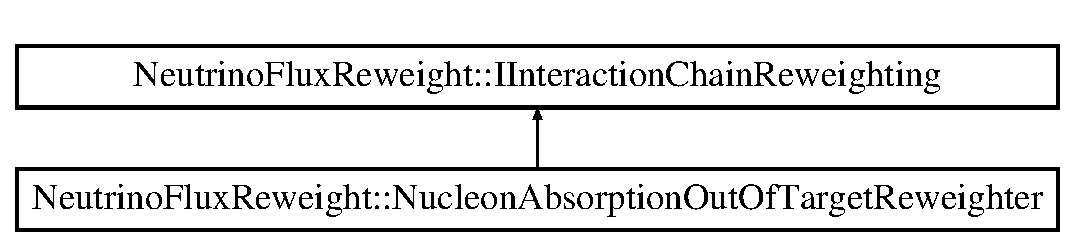
\includegraphics[height=2.000000cm]{class_neutrino_flux_reweight_1_1_nucleon_absorption_out_of_target_reweighter}
\end{center}
\end{figure}
\subsection*{Public Member Functions}
\begin{DoxyCompactItemize}
\item 
\hyperlink{class_neutrino_flux_reweight_1_1_nucleon_absorption_out_of_target_reweighter_a8195d5b2b35f7f1b7f8277556e0ed625}{Nucleon\-Absorption\-Out\-Of\-Target\-Reweighter} (int iuniv, const \hyperlink{class_neutrino_flux_reweight_1_1_parameter_table}{Parameter\-Table} \&cv\-\_\-pars, const \hyperlink{class_neutrino_flux_reweight_1_1_parameter_table}{Parameter\-Table} \&univ\-\_\-pars)
\item 
virtual \hyperlink{class_neutrino_flux_reweight_1_1_nucleon_absorption_out_of_target_reweighter_a4277a8f10a85466466ee10884b6e8f5f}{$\sim$\-Nucleon\-Absorption\-Out\-Of\-Target\-Reweighter} ()
\item 
virtual std\-::vector$<$ bool $>$ \hyperlink{class_neutrino_flux_reweight_1_1_nucleon_absorption_out_of_target_reweighter_a978c4e5458a827ff091c990b34515fb7}{can\-Reweight} (const \hyperlink{class_neutrino_flux_reweight_1_1_interaction_chain_data}{Interaction\-Chain\-Data} \&aa)
\begin{DoxyCompactList}\small\item\em Look through the \hyperlink{class_neutrino_flux_reweight_1_1_interaction_chain_data}{Interaction\-Chain\-Data} input and identify those Interactions that can be reweighted as part of a chain. We return a vector indicating which elements will be assigned a weight by calculate\-Weight. \end{DoxyCompactList}\item 
virtual double \hyperlink{class_neutrino_flux_reweight_1_1_nucleon_absorption_out_of_target_reweighter_a295719b84abffcab3d2cdf3a4aadb7b7}{calculate\-Weight} (const \hyperlink{class_neutrino_flux_reweight_1_1_interaction_chain_data}{Interaction\-Chain\-Data} \&aa)
\begin{DoxyCompactList}\small\item\em calculate a weight for this interaction chain given the central value parameters and the parameters for this universe. The weight is something like\-: f(cv)/f(M\-C) $\ast$ f(univ)/f(cv) where cv in this case corresponds to the best value of the parameter, given the data. If univ\-\_\-pars=cv\-\_\-pars then we are calculating a central value weight. Note, \hyperlink{class_neutrino_flux_reweight_1_1_nucleon_absorption_out_of_target_reweighter_a978c4e5458a827ff091c990b34515fb7}{can\-Reweight()} should be called to determine which elements of the chain are covered by the weight returned by \hyperlink{class_neutrino_flux_reweight_1_1_nucleon_absorption_out_of_target_reweighter_a295719b84abffcab3d2cdf3a4aadb7b7}{calculate\-Weight()} \end{DoxyCompactList}\end{DoxyCompactItemize}
\subsection*{Public Attributes}
\begin{DoxyCompactItemize}
\item 
const \hyperlink{class_neutrino_flux_reweight_1_1_parameter_table}{Parameter\-Table} \& \hyperlink{class_neutrino_flux_reweight_1_1_nucleon_absorption_out_of_target_reweighter_a15ea8c8b728192f7f61f2f7a503ea523}{cv\-Pars}
\item 
const \hyperlink{class_neutrino_flux_reweight_1_1_parameter_table}{Parameter\-Table} \& \hyperlink{class_neutrino_flux_reweight_1_1_nucleon_absorption_out_of_target_reweighter_afc305487c13ad3506ef55909e4e844ac}{univ\-Pars}
\end{DoxyCompactItemize}
\subsection*{Private Attributes}
\begin{DoxyCompactItemize}
\item 
int \hyperlink{class_neutrino_flux_reweight_1_1_nucleon_absorption_out_of_target_reweighter_a2b89b90d5bbc264d931574f752a51b7b}{i\-Univ}
\item 
float \hyperlink{class_neutrino_flux_reweight_1_1_nucleon_absorption_out_of_target_reweighter_a6e402e4d30132d0ccc65bc74e5add535}{inel\-\_\-pi\-Al\-\_\-xsec}
\end{DoxyCompactItemize}


\subsection{Detailed Description}
Reweight a M\-C survival probabiity when the particles through volumes. 

Definition at line 16 of file Nucleon\-Absorption\-Out\-Of\-Target\-Reweighter.\-h.



\subsection{Constructor \& Destructor Documentation}
\hypertarget{class_neutrino_flux_reweight_1_1_nucleon_absorption_out_of_target_reweighter_a8195d5b2b35f7f1b7f8277556e0ed625}{\index{Neutrino\-Flux\-Reweight\-::\-Nucleon\-Absorption\-Out\-Of\-Target\-Reweighter@{Neutrino\-Flux\-Reweight\-::\-Nucleon\-Absorption\-Out\-Of\-Target\-Reweighter}!Nucleon\-Absorption\-Out\-Of\-Target\-Reweighter@{Nucleon\-Absorption\-Out\-Of\-Target\-Reweighter}}
\index{Nucleon\-Absorption\-Out\-Of\-Target\-Reweighter@{Nucleon\-Absorption\-Out\-Of\-Target\-Reweighter}!NeutrinoFluxReweight::NucleonAbsorptionOutOfTargetReweighter@{Neutrino\-Flux\-Reweight\-::\-Nucleon\-Absorption\-Out\-Of\-Target\-Reweighter}}
\subsubsection[{Nucleon\-Absorption\-Out\-Of\-Target\-Reweighter}]{\setlength{\rightskip}{0pt plus 5cm}Neutrino\-Flux\-Reweight\-::\-Nucleon\-Absorption\-Out\-Of\-Target\-Reweighter\-::\-Nucleon\-Absorption\-Out\-Of\-Target\-Reweighter (
\begin{DoxyParamCaption}
\item[{int}]{iuniv, }
\item[{const {\bf Parameter\-Table} \&}]{cv\-\_\-pars, }
\item[{const {\bf Parameter\-Table} \&}]{univ\-\_\-pars}
\end{DoxyParamCaption}
)}}\label{class_neutrino_flux_reweight_1_1_nucleon_absorption_out_of_target_reweighter_a8195d5b2b35f7f1b7f8277556e0ed625}
The constructor. Note, we pass central value and single universe parameters in this constructor only. There is thus a 1 to 1 correspondence between an instance of this class and a given universe. 

Definition at line 12 of file Nucleon\-Absorption\-Out\-Of\-Target\-Reweighter.\-cpp.


\begin{DoxyCode}
12                                                                                                            
                                                    :\hyperlink{class_neutrino_flux_reweight_1_1_nucleon_absorption_out_of_target_reweighter_a15ea8c8b728192f7f61f2f7a503ea523}{cvPars}(cv\_pars),\hyperlink{class_neutrino_flux_reweight_1_1_nucleon_absorption_out_of_target_reweighter_afc305487c13ad3506ef55909e4e844ac}{univPars}(univ\_pars),
      \hyperlink{class_neutrino_flux_reweight_1_1_nucleon_absorption_out_of_target_reweighter_a2b89b90d5bbc264d931574f752a51b7b}{iUniv}(iuniv)\{ 
13 
14     \textcolor{comment}{// const boost::interprocess::flat\_map<std::string, double>& dsig\_table = univPars.getMap();}
15     \hyperlink{class_neutrino_flux_reweight_1_1_nucleon_absorption_out_of_target_reweighter_a6e402e4d30132d0ccc65bc74e5add535}{inel\_piAl\_xsec} = \hyperlink{class_neutrino_flux_reweight_1_1_nucleon_absorption_out_of_target_reweighter_afc305487c13ad3506ef55909e4e844ac}{univPars}.\hyperlink{class_neutrino_flux_reweight_1_1_parameter_table_acb7dc8335b65b116f6092f2fa57ca5ed}{getParameterValue}(\textcolor{stringliteral}{"inel\_piAl\_xsec"});
16 
17   \}
\end{DoxyCode}
\hypertarget{class_neutrino_flux_reweight_1_1_nucleon_absorption_out_of_target_reweighter_a4277a8f10a85466466ee10884b6e8f5f}{\index{Neutrino\-Flux\-Reweight\-::\-Nucleon\-Absorption\-Out\-Of\-Target\-Reweighter@{Neutrino\-Flux\-Reweight\-::\-Nucleon\-Absorption\-Out\-Of\-Target\-Reweighter}!$\sim$\-Nucleon\-Absorption\-Out\-Of\-Target\-Reweighter@{$\sim$\-Nucleon\-Absorption\-Out\-Of\-Target\-Reweighter}}
\index{$\sim$\-Nucleon\-Absorption\-Out\-Of\-Target\-Reweighter@{$\sim$\-Nucleon\-Absorption\-Out\-Of\-Target\-Reweighter}!NeutrinoFluxReweight::NucleonAbsorptionOutOfTargetReweighter@{Neutrino\-Flux\-Reweight\-::\-Nucleon\-Absorption\-Out\-Of\-Target\-Reweighter}}
\subsubsection[{$\sim$\-Nucleon\-Absorption\-Out\-Of\-Target\-Reweighter}]{\setlength{\rightskip}{0pt plus 5cm}Neutrino\-Flux\-Reweight\-::\-Nucleon\-Absorption\-Out\-Of\-Target\-Reweighter\-::$\sim$\-Nucleon\-Absorption\-Out\-Of\-Target\-Reweighter (
\begin{DoxyParamCaption}
{}
\end{DoxyParamCaption}
)\hspace{0.3cm}{\ttfamily [virtual]}}}\label{class_neutrino_flux_reweight_1_1_nucleon_absorption_out_of_target_reweighter_a4277a8f10a85466466ee10884b6e8f5f}


Definition at line 18 of file Nucleon\-Absorption\-Out\-Of\-Target\-Reweighter.\-cpp.


\begin{DoxyCode}
18                                                                                  \{
19     
20   \}
\end{DoxyCode}


\subsection{Member Function Documentation}
\hypertarget{class_neutrino_flux_reweight_1_1_nucleon_absorption_out_of_target_reweighter_a295719b84abffcab3d2cdf3a4aadb7b7}{\index{Neutrino\-Flux\-Reweight\-::\-Nucleon\-Absorption\-Out\-Of\-Target\-Reweighter@{Neutrino\-Flux\-Reweight\-::\-Nucleon\-Absorption\-Out\-Of\-Target\-Reweighter}!calculate\-Weight@{calculate\-Weight}}
\index{calculate\-Weight@{calculate\-Weight}!NeutrinoFluxReweight::NucleonAbsorptionOutOfTargetReweighter@{Neutrino\-Flux\-Reweight\-::\-Nucleon\-Absorption\-Out\-Of\-Target\-Reweighter}}
\subsubsection[{calculate\-Weight}]{\setlength{\rightskip}{0pt plus 5cm}double Neutrino\-Flux\-Reweight\-::\-Nucleon\-Absorption\-Out\-Of\-Target\-Reweighter\-::calculate\-Weight (
\begin{DoxyParamCaption}
\item[{const {\bf Interaction\-Chain\-Data} \&}]{aa}
\end{DoxyParamCaption}
)\hspace{0.3cm}{\ttfamily [virtual]}}}\label{class_neutrino_flux_reweight_1_1_nucleon_absorption_out_of_target_reweighter_a295719b84abffcab3d2cdf3a4aadb7b7}


calculate a weight for this interaction chain given the central value parameters and the parameters for this universe. The weight is something like\-: f(cv)/f(M\-C) $\ast$ f(univ)/f(cv) where cv in this case corresponds to the best value of the parameter, given the data. If univ\-\_\-pars=cv\-\_\-pars then we are calculating a central value weight. Note, \hyperlink{class_neutrino_flux_reweight_1_1_nucleon_absorption_out_of_target_reweighter_a978c4e5458a827ff091c990b34515fb7}{can\-Reweight()} should be called to determine which elements of the chain are covered by the weight returned by \hyperlink{class_neutrino_flux_reweight_1_1_nucleon_absorption_out_of_target_reweighter_a295719b84abffcab3d2cdf3a4aadb7b7}{calculate\-Weight()} 



Implements \hyperlink{class_neutrino_flux_reweight_1_1_i_interaction_chain_reweighting_ae28403553637013fdc720674ee24c7c5}{Neutrino\-Flux\-Reweight\-::\-I\-Interaction\-Chain\-Reweighting}.



Definition at line 40 of file Nucleon\-Absorption\-Out\-Of\-Target\-Reweighter.\-cpp.


\begin{DoxyCode}
40                                                                                               \{
41     
42     std::vector<ParticlesThroughVolumesData>  vec\_ptv = aa.ptv\_info;
43     \textcolor{keywordtype}{double} shift = \hyperlink{class_neutrino_flux_reweight_1_1_nucleon_absorption_out_of_target_reweighter_a6e402e4d30132d0ccc65bc74e5add535}{inel\_piAl\_xsec};
44     
45     \textcolor{keywordtype}{double} NA\_mb    = 6.02E-4;
46     \textcolor{keywordtype}{double} wgt      = 1.0;
47     \textcolor{keywordtype}{double} tot\_dist = 0.0;
48     \textcolor{keywordtype}{double} low\_val  = 1.E-20;   
49     
50     \textcolor{keywordflow}{for}(\textcolor{keywordtype}{int} index\_vol =0;index\_vol<3;index\_vol++)\{
51       \textcolor{keywordflow}{for}(\textcolor{keywordtype}{int} ii=0;ii<3;ii++)\{  
52         tot\_dist = vec\_ptv[index\_vol].AmountMat[ii];
53         \textcolor{keywordflow}{if}(tot\_dist<low\_val)\textcolor{keywordflow}{continue};
54         \textcolor{keywordflow}{if}(vec\_ptv[index\_vol].Pdgs[ii]!=2212 && vec\_ptv[index\_vol].Pdgs[ii]!=2112) \textcolor{keywordflow}{continue};    
55         tot\_dist *= NA\_mb;
56         tot\_dist *= shift;
57         wgt *= exp(-1.0*tot\_dist);   
58       \}
59     \}
60     
61     \textcolor{keywordflow}{return} wgt;
62     
63   \}
\end{DoxyCode}
\hypertarget{class_neutrino_flux_reweight_1_1_nucleon_absorption_out_of_target_reweighter_a978c4e5458a827ff091c990b34515fb7}{\index{Neutrino\-Flux\-Reweight\-::\-Nucleon\-Absorption\-Out\-Of\-Target\-Reweighter@{Neutrino\-Flux\-Reweight\-::\-Nucleon\-Absorption\-Out\-Of\-Target\-Reweighter}!can\-Reweight@{can\-Reweight}}
\index{can\-Reweight@{can\-Reweight}!NeutrinoFluxReweight::NucleonAbsorptionOutOfTargetReweighter@{Neutrino\-Flux\-Reweight\-::\-Nucleon\-Absorption\-Out\-Of\-Target\-Reweighter}}
\subsubsection[{can\-Reweight}]{\setlength{\rightskip}{0pt plus 5cm}std\-::vector$<$ bool $>$ Neutrino\-Flux\-Reweight\-::\-Nucleon\-Absorption\-Out\-Of\-Target\-Reweighter\-::can\-Reweight (
\begin{DoxyParamCaption}
\item[{const {\bf Interaction\-Chain\-Data} \&}]{aa}
\end{DoxyParamCaption}
)\hspace{0.3cm}{\ttfamily [virtual]}}}\label{class_neutrino_flux_reweight_1_1_nucleon_absorption_out_of_target_reweighter_a978c4e5458a827ff091c990b34515fb7}


Look through the \hyperlink{class_neutrino_flux_reweight_1_1_interaction_chain_data}{Interaction\-Chain\-Data} input and identify those Interactions that can be reweighted as part of a chain. We return a vector indicating which elements will be assigned a weight by calculate\-Weight. 



Implements \hyperlink{class_neutrino_flux_reweight_1_1_i_interaction_chain_reweighting_aacf17580c1d316f0ebcdfdff7418e9e3}{Neutrino\-Flux\-Reweight\-::\-I\-Interaction\-Chain\-Reweighting}.



Definition at line 21 of file Nucleon\-Absorption\-Out\-Of\-Target\-Reweighter.\-cpp.


\begin{DoxyCode}
21                                                                                                    \{
22  
23     std::vector<bool> this\_nodes;
24     \textcolor{comment}{//int index\_vol = 0;}
25     \textcolor{keywordtype}{double} low\_val = 1.E-20;    
26   
27     std::vector<ParticlesThroughVolumesData>  vec\_ptv = aa.ptv\_info;
28 
29     \textcolor{keywordtype}{bool} passVOL = \textcolor{keyword}{false};
30     \textcolor{comment}{//Cheking at least one ancestor with amount of materail value:}
31     \textcolor{keywordflow}{for}(\textcolor{keywordtype}{int} index\_vol =0;index\_vol<3;index\_vol++)\{
32       \textcolor{keywordflow}{for}(\textcolor{keywordtype}{int} ii=0;ii<3;ii++)\{
33         passVOL = passVOL || (vec\_ptv[index\_vol].AmountMat[ii] >low\_val && (vec\_ptv[index\_vol].Pdgs[ii]==
      2212 || vec\_ptv[index\_vol].Pdgs[ii]==2112));
34       \}
35     \}
36     this\_nodes.push\_back(passVOL);
37     \textcolor{keywordflow}{return} this\_nodes;
38     
39   \}
\end{DoxyCode}


\subsection{Member Data Documentation}
\hypertarget{class_neutrino_flux_reweight_1_1_nucleon_absorption_out_of_target_reweighter_a15ea8c8b728192f7f61f2f7a503ea523}{\index{Neutrino\-Flux\-Reweight\-::\-Nucleon\-Absorption\-Out\-Of\-Target\-Reweighter@{Neutrino\-Flux\-Reweight\-::\-Nucleon\-Absorption\-Out\-Of\-Target\-Reweighter}!cv\-Pars@{cv\-Pars}}
\index{cv\-Pars@{cv\-Pars}!NeutrinoFluxReweight::NucleonAbsorptionOutOfTargetReweighter@{Neutrino\-Flux\-Reweight\-::\-Nucleon\-Absorption\-Out\-Of\-Target\-Reweighter}}
\subsubsection[{cv\-Pars}]{\setlength{\rightskip}{0pt plus 5cm}const {\bf Parameter\-Table}\& Neutrino\-Flux\-Reweight\-::\-Nucleon\-Absorption\-Out\-Of\-Target\-Reweighter\-::cv\-Pars}}\label{class_neutrino_flux_reweight_1_1_nucleon_absorption_out_of_target_reweighter_a15ea8c8b728192f7f61f2f7a503ea523}


Definition at line 27 of file Nucleon\-Absorption\-Out\-Of\-Target\-Reweighter.\-h.

\hypertarget{class_neutrino_flux_reweight_1_1_nucleon_absorption_out_of_target_reweighter_a6e402e4d30132d0ccc65bc74e5add535}{\index{Neutrino\-Flux\-Reweight\-::\-Nucleon\-Absorption\-Out\-Of\-Target\-Reweighter@{Neutrino\-Flux\-Reweight\-::\-Nucleon\-Absorption\-Out\-Of\-Target\-Reweighter}!inel\-\_\-pi\-Al\-\_\-xsec@{inel\-\_\-pi\-Al\-\_\-xsec}}
\index{inel\-\_\-pi\-Al\-\_\-xsec@{inel\-\_\-pi\-Al\-\_\-xsec}!NeutrinoFluxReweight::NucleonAbsorptionOutOfTargetReweighter@{Neutrino\-Flux\-Reweight\-::\-Nucleon\-Absorption\-Out\-Of\-Target\-Reweighter}}
\subsubsection[{inel\-\_\-pi\-Al\-\_\-xsec}]{\setlength{\rightskip}{0pt plus 5cm}float Neutrino\-Flux\-Reweight\-::\-Nucleon\-Absorption\-Out\-Of\-Target\-Reweighter\-::inel\-\_\-pi\-Al\-\_\-xsec\hspace{0.3cm}{\ttfamily [private]}}}\label{class_neutrino_flux_reweight_1_1_nucleon_absorption_out_of_target_reweighter_a6e402e4d30132d0ccc65bc74e5add535}


Definition at line 31 of file Nucleon\-Absorption\-Out\-Of\-Target\-Reweighter.\-h.

\hypertarget{class_neutrino_flux_reweight_1_1_nucleon_absorption_out_of_target_reweighter_a2b89b90d5bbc264d931574f752a51b7b}{\index{Neutrino\-Flux\-Reweight\-::\-Nucleon\-Absorption\-Out\-Of\-Target\-Reweighter@{Neutrino\-Flux\-Reweight\-::\-Nucleon\-Absorption\-Out\-Of\-Target\-Reweighter}!i\-Univ@{i\-Univ}}
\index{i\-Univ@{i\-Univ}!NeutrinoFluxReweight::NucleonAbsorptionOutOfTargetReweighter@{Neutrino\-Flux\-Reweight\-::\-Nucleon\-Absorption\-Out\-Of\-Target\-Reweighter}}
\subsubsection[{i\-Univ}]{\setlength{\rightskip}{0pt plus 5cm}int Neutrino\-Flux\-Reweight\-::\-Nucleon\-Absorption\-Out\-Of\-Target\-Reweighter\-::i\-Univ\hspace{0.3cm}{\ttfamily [private]}}}\label{class_neutrino_flux_reweight_1_1_nucleon_absorption_out_of_target_reweighter_a2b89b90d5bbc264d931574f752a51b7b}


Definition at line 30 of file Nucleon\-Absorption\-Out\-Of\-Target\-Reweighter.\-h.

\hypertarget{class_neutrino_flux_reweight_1_1_nucleon_absorption_out_of_target_reweighter_afc305487c13ad3506ef55909e4e844ac}{\index{Neutrino\-Flux\-Reweight\-::\-Nucleon\-Absorption\-Out\-Of\-Target\-Reweighter@{Neutrino\-Flux\-Reweight\-::\-Nucleon\-Absorption\-Out\-Of\-Target\-Reweighter}!univ\-Pars@{univ\-Pars}}
\index{univ\-Pars@{univ\-Pars}!NeutrinoFluxReweight::NucleonAbsorptionOutOfTargetReweighter@{Neutrino\-Flux\-Reweight\-::\-Nucleon\-Absorption\-Out\-Of\-Target\-Reweighter}}
\subsubsection[{univ\-Pars}]{\setlength{\rightskip}{0pt plus 5cm}const {\bf Parameter\-Table}\& Neutrino\-Flux\-Reweight\-::\-Nucleon\-Absorption\-Out\-Of\-Target\-Reweighter\-::univ\-Pars}}\label{class_neutrino_flux_reweight_1_1_nucleon_absorption_out_of_target_reweighter_afc305487c13ad3506ef55909e4e844ac}


Definition at line 28 of file Nucleon\-Absorption\-Out\-Of\-Target\-Reweighter.\-h.



The documentation for this class was generated from the following files\-:\begin{DoxyCompactItemize}
\item 
include/\hyperlink{_nucleon_absorption_out_of_target_reweighter_8h}{Nucleon\-Absorption\-Out\-Of\-Target\-Reweighter.\-h}\item 
src/\hyperlink{_nucleon_absorption_out_of_target_reweighter_8cpp}{Nucleon\-Absorption\-Out\-Of\-Target\-Reweighter.\-cpp}\end{DoxyCompactItemize}

\hypertarget{class_numi2_pdg}{\section{Numi2\-Pdg Class Reference}
\label{class_numi2_pdg}\index{Numi2\-Pdg@{Numi2\-Pdg}}
}


{\ttfamily \#include $<$Numi2\-Pdg.\-h$>$}

\subsection*{Public Member Functions}
\begin{DoxyCompactItemize}
\item 
\hyperlink{class_numi2_pdg_ae30fd995460ae57c3a0b0de6d4485991}{Numi2\-Pdg} ()
\item 
virtual \hyperlink{class_numi2_pdg_a1afb642b492342a70ccb05fb7b0d199d}{$\sim$\-Numi2\-Pdg} ()
\item 
int \hyperlink{class_numi2_pdg_ac8d5438ffd52928a82738feed56e4f90}{Get\-Pdg} (int numipart)
\end{DoxyCompactItemize}


\subsection{Detailed Description}
Convert numi particle id number to pdg codes 

Definition at line 6 of file Numi2\-Pdg.\-h.



\subsection{Constructor \& Destructor Documentation}
\hypertarget{class_numi2_pdg_ae30fd995460ae57c3a0b0de6d4485991}{\index{Numi2\-Pdg@{Numi2\-Pdg}!Numi2\-Pdg@{Numi2\-Pdg}}
\index{Numi2\-Pdg@{Numi2\-Pdg}!Numi2Pdg@{Numi2\-Pdg}}
\subsubsection[{Numi2\-Pdg}]{\setlength{\rightskip}{0pt plus 5cm}Numi2\-Pdg\-::\-Numi2\-Pdg (
\begin{DoxyParamCaption}
{}
\end{DoxyParamCaption}
)}}\label{class_numi2_pdg_ae30fd995460ae57c3a0b0de6d4485991}


Definition at line 4 of file Numi2\-Pdg.\-cpp.


\begin{DoxyCode}
4                   \{
5   
6 \}
\end{DoxyCode}
\hypertarget{class_numi2_pdg_a1afb642b492342a70ccb05fb7b0d199d}{\index{Numi2\-Pdg@{Numi2\-Pdg}!$\sim$\-Numi2\-Pdg@{$\sim$\-Numi2\-Pdg}}
\index{$\sim$\-Numi2\-Pdg@{$\sim$\-Numi2\-Pdg}!Numi2Pdg@{Numi2\-Pdg}}
\subsubsection[{$\sim$\-Numi2\-Pdg}]{\setlength{\rightskip}{0pt plus 5cm}Numi2\-Pdg\-::$\sim$\-Numi2\-Pdg (
\begin{DoxyParamCaption}
{}
\end{DoxyParamCaption}
)\hspace{0.3cm}{\ttfamily [virtual]}}}\label{class_numi2_pdg_a1afb642b492342a70ccb05fb7b0d199d}


Definition at line 83 of file Numi2\-Pdg.\-cpp.


\begin{DoxyCode}
83                    \{
84   
85 \}
\end{DoxyCode}


\subsection{Member Function Documentation}
\hypertarget{class_numi2_pdg_ac8d5438ffd52928a82738feed56e4f90}{\index{Numi2\-Pdg@{Numi2\-Pdg}!Get\-Pdg@{Get\-Pdg}}
\index{Get\-Pdg@{Get\-Pdg}!Numi2Pdg@{Numi2\-Pdg}}
\subsubsection[{Get\-Pdg}]{\setlength{\rightskip}{0pt plus 5cm}int Numi2\-Pdg\-::\-Get\-Pdg (
\begin{DoxyParamCaption}
\item[{int}]{numipart}
\end{DoxyParamCaption}
)}}\label{class_numi2_pdg_ac8d5438ffd52928a82738feed56e4f90}
Get Pdg code from Numi codes(Fluka?) 

Definition at line 8 of file Numi2\-Pdg.\-cpp.


\begin{DoxyCode}
8                                 \{
9   
10   \textcolor{keywordtype}{int} pdg = 0;
11   
12   \textcolor{keywordflow}{switch}(numipart)\{
13   \textcolor{keywordflow}{case} 5:
14     pdg = -13; \textcolor{keywordflow}{break};
15   \textcolor{keywordflow}{case} 6:
16     pdg =  13; \textcolor{keywordflow}{break};
17   \textcolor{keywordflow}{case} 7:
18     pdg = 111; \textcolor{keywordflow}{break};
19   \textcolor{keywordflow}{case} 8:
20     pdg = 211; \textcolor{keywordflow}{break};  
21   \textcolor{keywordflow}{case} 9:
22     pdg = -211; \textcolor{keywordflow}{break}; 
23   \textcolor{keywordflow}{case} 10:
24     pdg = 130; \textcolor{keywordflow}{break};
25   \textcolor{keywordflow}{case} 11:
26     pdg = 321; \textcolor{keywordflow}{break};
27   \textcolor{keywordflow}{case} 12:
28     pdg = -321; \textcolor{keywordflow}{break};
29   \textcolor{keywordflow}{case} 13:
30     pdg = 2112; \textcolor{keywordflow}{break};  
31   \textcolor{keywordflow}{case} 14:
32     pdg = 2212; \textcolor{keywordflow}{break};
33   \textcolor{keywordflow}{case} 15:
34     pdg = -2212; \textcolor{keywordflow}{break};
35   \textcolor{keywordflow}{case} 16:
36     pdg = 310; \textcolor{keywordflow}{break};
37   \textcolor{keywordflow}{case} 17:
38     pdg = 221; \textcolor{keywordflow}{break};
39   \textcolor{keywordflow}{case} 18:
40     pdg = 3122; \textcolor{keywordflow}{break};  
41   \textcolor{keywordflow}{case} 19:
42     pdg = 3222; \textcolor{keywordflow}{break};
43   \textcolor{keywordflow}{case} 20:
44     pdg = 3212; \textcolor{keywordflow}{break};
45   \textcolor{keywordflow}{case} 21:
46     pdg = 3112; \textcolor{keywordflow}{break};
47   \textcolor{keywordflow}{case} 22:
48     pdg = 3322; \textcolor{keywordflow}{break};
49   \textcolor{keywordflow}{case} 23:
50     pdg = 3312; \textcolor{keywordflow}{break};  
51   \textcolor{keywordflow}{case} 24:
52     pdg = 3334; \textcolor{keywordflow}{break};
53   \textcolor{keywordflow}{case} 25:
54     pdg = -2112; \textcolor{keywordflow}{break};
55   \textcolor{keywordflow}{case} 26:
56     pdg = -3122; \textcolor{keywordflow}{break};
57   \textcolor{keywordflow}{case} 27:
58     pdg = -3112; \textcolor{keywordflow}{break};
59   \textcolor{keywordflow}{case} 28:
60     pdg = -3212; \textcolor{keywordflow}{break};  
61   \textcolor{keywordflow}{case} 29:
62     pdg = -3222; \textcolor{keywordflow}{break};
63   \textcolor{keywordflow}{case} 30:
64     pdg = -3322; \textcolor{keywordflow}{break};
65   \textcolor{keywordflow}{case} 31:
66     pdg = -3312; \textcolor{keywordflow}{break};
67   \textcolor{keywordflow}{case} 52:
68     pdg = -12; \textcolor{keywordflow}{break};
69   \textcolor{keywordflow}{case} 53:
70     pdg = 12; \textcolor{keywordflow}{break};  
71   \textcolor{keywordflow}{case} 55:
72     pdg = -14;  \textcolor{keywordflow}{break};
73   \textcolor{keywordflow}{case} 56:
74     pdg = 14; \textcolor{keywordflow}{break};
75   \textcolor{keywordflow}{case} 99:
76     pdg = 0; \textcolor{keywordflow}{break};
77   \}  
78 
79   \textcolor{keywordflow}{return} pdg;
80 
81 \}
\end{DoxyCode}


The documentation for this class was generated from the following files\-:\begin{DoxyCompactItemize}
\item 
include/\hyperlink{_numi2_pdg_8h}{Numi2\-Pdg.\-h}\item 
src/\hyperlink{_numi2_pdg_8cpp}{Numi2\-Pdg.\-cpp}\end{DoxyCompactItemize}

\hypertarget{class_neutrino_flux_auxiliar_1_1_nu_weight}{\section{Neutrino\-Flux\-Auxiliar\-:\-:Nu\-Weight Class Reference}
\label{class_neutrino_flux_auxiliar_1_1_nu_weight}\index{Neutrino\-Flux\-Auxiliar\-::\-Nu\-Weight@{Neutrino\-Flux\-Auxiliar\-::\-Nu\-Weight}}
}


Get the weight to get the neutrino probability flux in one point.  




{\ttfamily \#include $<$Nu\-Weight.\-h$>$}

\subsection*{Public Member Functions}
\begin{DoxyCompactItemize}
\item 
\hyperlink{class_neutrino_flux_auxiliar_1_1_nu_weight_a8b1c902f732e7be8d3591e74c807fb3c}{Nu\-Weight} (std\-::vector$<$ double $>$ \&posdet)
\begin{DoxyCompactList}\small\item\em The constructor has to have the position of the detector. \end{DoxyCompactList}\item 
\hyperlink{class_neutrino_flux_auxiliar_1_1_nu_weight_a1ee7ff5745a68e9595751fd4f16b66ec}{$\sim$\-Nu\-Weight} ()
\begin{DoxyCompactList}\small\item\em Destructor. \end{DoxyCompactList}\item 
void \hyperlink{class_neutrino_flux_auxiliar_1_1_nu_weight_ac6b650be51f799539e2f5ddddf3256ba}{calculate\-\_\-weight} (bsim\-::\-Dk2\-Nu $\ast$nu)
\begin{DoxyCompactList}\small\item\em Calculate weight based on dk2nu entry. After this, enu and wgt have meaningful values. \end{DoxyCompactList}\end{DoxyCompactItemize}
\subsection*{Public Attributes}
\begin{DoxyCompactItemize}
\item 
double \hyperlink{class_neutrino_flux_auxiliar_1_1_nu_weight_aaf30ef23c7cf98ecbda310a777d0b8aa}{enu}
\item 
double \hyperlink{class_neutrino_flux_auxiliar_1_1_nu_weight_a53e3e4d489356d71c6493e9e4ae11250}{wgt}
\end{DoxyCompactItemize}
\subsection*{Private Attributes}
\begin{DoxyCompactItemize}
\item 
T\-Database\-P\-D\-G $\ast$ \hyperlink{class_neutrino_flux_auxiliar_1_1_nu_weight_aa35fc1d624cd975a9657f1a081a776ca}{particle}
\item 
double \hyperlink{class_neutrino_flux_auxiliar_1_1_nu_weight_a9ea8df1e61c18a5a795746c182c31a5a}{xdet}
\item 
double \hyperlink{class_neutrino_flux_auxiliar_1_1_nu_weight_a4041206ba690070b210e5d8b28497c56}{ydet}
\item 
double \hyperlink{class_neutrino_flux_auxiliar_1_1_nu_weight_a4e33b89875dd565737b9a35e201b4585}{zdet}
\end{DoxyCompactItemize}


\subsection{Detailed Description}
Get the weight to get the neutrino probability flux in one point. 

Definition at line 19 of file Nu\-Weight.\-h.



\subsection{Constructor \& Destructor Documentation}
\hypertarget{class_neutrino_flux_auxiliar_1_1_nu_weight_a8b1c902f732e7be8d3591e74c807fb3c}{\index{Neutrino\-Flux\-Auxiliar\-::\-Nu\-Weight@{Neutrino\-Flux\-Auxiliar\-::\-Nu\-Weight}!Nu\-Weight@{Nu\-Weight}}
\index{Nu\-Weight@{Nu\-Weight}!NeutrinoFluxAuxiliar::NuWeight@{Neutrino\-Flux\-Auxiliar\-::\-Nu\-Weight}}
\subsubsection[{Nu\-Weight}]{\setlength{\rightskip}{0pt plus 5cm}Neutrino\-Flux\-Auxiliar\-::\-Nu\-Weight\-::\-Nu\-Weight (
\begin{DoxyParamCaption}
\item[{std\-::vector$<$ double $>$ \&}]{posdet}
\end{DoxyParamCaption}
)}}\label{class_neutrino_flux_auxiliar_1_1_nu_weight_a8b1c902f732e7be8d3591e74c807fb3c}


The constructor has to have the position of the detector. 



Definition at line 7 of file Nu\-Weight.\-cpp.


\begin{DoxyCode}
7                                              \{
8     
9     \hyperlink{class_neutrino_flux_auxiliar_1_1_nu_weight_aa35fc1d624cd975a9657f1a081a776ca}{particle} = TDatabasePDG::Instance();
10     \hyperlink{class_neutrino_flux_auxiliar_1_1_nu_weight_aaf30ef23c7cf98ecbda310a777d0b8aa}{NuWeight::enu}  = -1.0;
11     \hyperlink{class_neutrino_flux_auxiliar_1_1_nu_weight_a53e3e4d489356d71c6493e9e4ae11250}{NuWeight::wgt}  = -1.0;
12     \hyperlink{class_neutrino_flux_auxiliar_1_1_nu_weight_a9ea8df1e61c18a5a795746c182c31a5a}{xdet} = posdet[0];
13     \hyperlink{class_neutrino_flux_auxiliar_1_1_nu_weight_a4041206ba690070b210e5d8b28497c56}{ydet} = posdet[1];    
14     \hyperlink{class_neutrino_flux_auxiliar_1_1_nu_weight_a4e33b89875dd565737b9a35e201b4585}{zdet} = posdet[2];
15   \}
\end{DoxyCode}
\hypertarget{class_neutrino_flux_auxiliar_1_1_nu_weight_a1ee7ff5745a68e9595751fd4f16b66ec}{\index{Neutrino\-Flux\-Auxiliar\-::\-Nu\-Weight@{Neutrino\-Flux\-Auxiliar\-::\-Nu\-Weight}!$\sim$\-Nu\-Weight@{$\sim$\-Nu\-Weight}}
\index{$\sim$\-Nu\-Weight@{$\sim$\-Nu\-Weight}!NeutrinoFluxAuxiliar::NuWeight@{Neutrino\-Flux\-Auxiliar\-::\-Nu\-Weight}}
\subsubsection[{$\sim$\-Nu\-Weight}]{\setlength{\rightskip}{0pt plus 5cm}Neutrino\-Flux\-Auxiliar\-::\-Nu\-Weight\-::$\sim$\-Nu\-Weight (
\begin{DoxyParamCaption}
{}
\end{DoxyParamCaption}
)}}\label{class_neutrino_flux_auxiliar_1_1_nu_weight_a1ee7ff5745a68e9595751fd4f16b66ec}


Destructor. 



Definition at line 118 of file Nu\-Weight.\-cpp.


\begin{DoxyCode}
118                      \{ 
119   \}
\end{DoxyCode}


\subsection{Member Function Documentation}
\hypertarget{class_neutrino_flux_auxiliar_1_1_nu_weight_ac6b650be51f799539e2f5ddddf3256ba}{\index{Neutrino\-Flux\-Auxiliar\-::\-Nu\-Weight@{Neutrino\-Flux\-Auxiliar\-::\-Nu\-Weight}!calculate\-\_\-weight@{calculate\-\_\-weight}}
\index{calculate\-\_\-weight@{calculate\-\_\-weight}!NeutrinoFluxAuxiliar::NuWeight@{Neutrino\-Flux\-Auxiliar\-::\-Nu\-Weight}}
\subsubsection[{calculate\-\_\-weight}]{\setlength{\rightskip}{0pt plus 5cm}void Neutrino\-Flux\-Auxiliar\-::\-Nu\-Weight\-::calculate\-\_\-weight (
\begin{DoxyParamCaption}
\item[{bsim\-::\-Dk2\-Nu $\ast$}]{nu}
\end{DoxyParamCaption}
)}}\label{class_neutrino_flux_auxiliar_1_1_nu_weight_ac6b650be51f799539e2f5ddddf3256ba}


Calculate weight based on dk2nu entry. After this, enu and wgt have meaningful values. 



Definition at line 16 of file Nu\-Weight.\-cpp.


\begin{DoxyCode}
16                                               \{
17      \textcolor{comment}{//assumes units are GeV and cm}
18 
19     \textcolor{keywordtype}{int} likely\_ion = 100000000;
20     \textcolor{keywordtype}{double} mpar=-1.;
21     \textcolor{keywordtype}{int} size = (nu->ancestor).size();
22     \textcolor{keywordtype}{int} pdg = nu->ancestor[size-2].pdg;
23 
24     \textcolor{keywordflow}{if}(pdg>likely\_ion || pdg<-1*likely\_ion)\{
25       std::cout<< \textcolor{stringliteral}{"Not handling ions yet, pdg: "}<<pdg<<std::endl;
26       exit (1);
27     \}
28     \textcolor{keywordflow}{else}\{
29       mpar = \hyperlink{class_neutrino_flux_auxiliar_1_1_nu_weight_aa35fc1d624cd975a9657f1a081a776ca}{particle}->GetParticle(pdg)->Mass();
30     \}
31     
32     \textcolor{keywordtype}{double} ppar  = sqrt( pow(nu->decay.pdpx,2) + pow(nu->decay.pdpy,2) + pow(nu->decay.pdpz,2) );
33     \textcolor{keywordtype}{double} epar  = sqrt(pow(ppar,2)+pow(mpar,2));
34     \textcolor{keywordtype}{double} gamma = epar / mpar;
35     \textcolor{keywordtype}{double} beta = sqrt(pow(gamma,2)-1)/gamma;
36 
37     \textcolor{keywordtype}{double} rr = sqrt(pow(\hyperlink{class_neutrino_flux_auxiliar_1_1_nu_weight_a9ea8df1e61c18a5a795746c182c31a5a}{xdet}-nu->decay.vx,2)+pow(\hyperlink{class_neutrino_flux_auxiliar_1_1_nu_weight_a4041206ba690070b210e5d8b28497c56}{ydet}-nu->decay.vy,2)+pow(
      \hyperlink{class_neutrino_flux_auxiliar_1_1_nu_weight_a4e33b89875dd565737b9a35e201b4585}{zdet}-nu->decay.vz,2));
38     \textcolor{keywordtype}{double} cos\_theta = ( (nu->decay.pdpx)*(\hyperlink{class_neutrino_flux_auxiliar_1_1_nu_weight_a9ea8df1e61c18a5a795746c182c31a5a}{xdet}-nu->decay.vx) + (nu->decay.pdpy)*(
      \hyperlink{class_neutrino_flux_auxiliar_1_1_nu_weight_a4041206ba690070b210e5d8b28497c56}{ydet}-nu->decay.vy) + (nu->decay.pdpz)*(\hyperlink{class_neutrino_flux_auxiliar_1_1_nu_weight_a4e33b89875dd565737b9a35e201b4585}{zdet}-nu->decay.vz) )/ (ppar*rr);
39  
40     \textcolor{keywordflow}{if}(cos\_theta > 1 || cos\_theta < -1)\{
41       std::cout<< \textcolor{stringliteral}{"Cosine of neutrino not allowed: "}<<cos\_theta<<std::endl;
42       exit (1);
43     \}
44     \textcolor{keywordtype}{double} MM      = 1.0/(gamma*(1.0-beta*cos\_theta));
45     \textcolor{keywordtype}{double} angdet  = (pow(\hyperlink{_nu_weight_8cpp_ae7afe156db7f7ccfcf48729eb3817b69}{rdet},2) /pow(rr,2)/ 4.); 
46     \hyperlink{class_neutrino_flux_auxiliar_1_1_nu_weight_aaf30ef23c7cf98ecbda310a777d0b8aa}{NuWeight::enu}  =  MM*(nu->decay.necm);
47     \hyperlink{class_neutrino_flux_auxiliar_1_1_nu_weight_a53e3e4d489356d71c6493e9e4ae11250}{NuWeight::wgt}  = angdet * pow(MM,2);
48  
49     \textcolor{comment}{//done for all except polarized muon}
50     \textcolor{comment}{// in which case need to modify weight}
51     \textcolor{keywordflow}{if} (pdg == 13 || pdg == -13)\{
52 
53       \textcolor{comment}{//boost new neutrino to mu decay cm}
54       \textcolor{keywordtype}{double} vbeta[3];
55       vbeta[0] = nu->decay.pdpx / epar;
56       vbeta[1] = nu->decay.pdpy / epar;
57       vbeta[2] = nu->decay.pdpz / epar;
58 
59       \textcolor{keywordtype}{double} p\_nu[3]; \textcolor{comment}{//nu momentum    }
60       p\_nu[0] = (\hyperlink{class_neutrino_flux_auxiliar_1_1_nu_weight_a9ea8df1e61c18a5a795746c182c31a5a}{xdet}- nu->decay.vx) * (\hyperlink{class_neutrino_flux_auxiliar_1_1_nu_weight_aaf30ef23c7cf98ecbda310a777d0b8aa}{NuWeight::enu}) / rr;
61       p\_nu[1] = (\hyperlink{class_neutrino_flux_auxiliar_1_1_nu_weight_a4041206ba690070b210e5d8b28497c56}{ydet}- nu->decay.vy) * (\hyperlink{class_neutrino_flux_auxiliar_1_1_nu_weight_aaf30ef23c7cf98ecbda310a777d0b8aa}{NuWeight::enu}) / rr;
62       p\_nu[2] = (\hyperlink{class_neutrino_flux_auxiliar_1_1_nu_weight_a4e33b89875dd565737b9a35e201b4585}{zdet}- nu->decay.vz) * (\hyperlink{class_neutrino_flux_auxiliar_1_1_nu_weight_aaf30ef23c7cf98ecbda310a777d0b8aa}{NuWeight::enu}) / rr;
63 
64       \textcolor{keywordtype}{double} partial = gamma*(vbeta[0]*p\_nu[0]+vbeta[1]*p\_nu[1]+vbeta[2]*p\_nu[2]);
65       partial = (\hyperlink{class_neutrino_flux_auxiliar_1_1_nu_weight_aaf30ef23c7cf98ecbda310a777d0b8aa}{NuWeight::enu})-partial / (gamma+1.);
66 
67       \textcolor{keywordtype}{double} p\_dcm\_nu[4];
68       \textcolor{keywordflow}{for} (\textcolor{keywordtype}{int} i=0;i<3;i++) p\_dcm\_nu[i]=p\_nu[i]-vbeta[i]*gamma*partial;
69       p\_dcm\_nu[3]=0.;
70       \textcolor{keywordflow}{for} (\textcolor{keywordtype}{int} i=0;i<3;i++) p\_dcm\_nu[3]+=p\_dcm\_nu[i]*p\_dcm\_nu[i];
71       p\_dcm\_nu[3]=sqrt(p\_dcm\_nu[3]);
72 
73       \textcolor{comment}{//boost parent of mu to mu production cm}
74       gamma   = nu->decay.ppenergy / mpar;
75       vbeta[0] = nu->decay.ppdxdz * nu->decay.pppz / nu->decay.ppenergy;
76       vbeta[1] = nu->decay.ppdydz * nu->decay.pppz / nu->decay.ppenergy;
77       vbeta[2] =                    nu->decay.pppz / nu->decay.ppenergy;
78       partial = gamma*(vbeta[0]*nu->decay.muparpx+vbeta[1]*nu->decay.muparpy+vbeta[2]*nu->decay.muparpz);
79       partial = nu->decay.mupare - partial / (gamma+1.);
80 
81       \textcolor{keywordtype}{double} p\_pcm\_mp[4];
82       p\_pcm\_mp[0]=nu->decay.muparpx-vbeta[0]*gamma*partial;
83       p\_pcm\_mp[1]=nu->decay.muparpy-vbeta[1]*gamma*partial;
84       p\_pcm\_mp[2]=nu->decay.muparpz-vbeta[2]*gamma*partial;
85       p\_pcm\_mp[3]=0.;
86       \textcolor{keywordflow}{for} (\textcolor{keywordtype}{int} i=0;i<3;i++) p\_pcm\_mp[3]+=p\_pcm\_mp[i]*p\_pcm\_mp[i];
87       p\_pcm\_mp[3]=sqrt(p\_pcm\_mp[3]);
88 
89       \textcolor{keywordtype}{double} wt\_ratio = 1.;
90       \textcolor{comment}{//have to check p\_pcm\_mp}
91       \textcolor{comment}{//it can be 0 if mupar..=0. (I guess muons created in target??)}
92       \textcolor{keywordflow}{if} (p\_pcm\_mp[3] != 0. ) \{
93         \textcolor{comment}{//calc new decay angle w.r.t. (anti)spin direction}
94         \textcolor{keywordtype}{double} costh = (p\_dcm\_nu[0]*p\_pcm\_mp[0]+ 
95                         p\_dcm\_nu[1]*p\_pcm\_mp[1]+ 
96                         p\_dcm\_nu[2]*p\_pcm\_mp[2])/(p\_dcm\_nu[3]*p\_pcm\_mp[3]);
97 
98         \textcolor{keywordflow}{if} (costh>1.) costh = 1.;
99         \textcolor{keywordflow}{else} \textcolor{keywordflow}{if} (costh<-1.) costh = -1.;
100 
101         \textcolor{comment}{//calc relative weight due to angle difference}
102         \textcolor{keywordflow}{if}(nu->decay.ntype == 12 || nu->decay.ntype == -12)\{
103           wt\_ratio = 1.-costh;
104         \}
105         \textcolor{keywordflow}{else} \textcolor{keywordflow}{if}(nu->decay.ntype == 14 || nu->decay.ntype == -14)\{
106           \textcolor{keywordtype}{double} mumass = \hyperlink{class_neutrino_flux_auxiliar_1_1_nu_weight_aa35fc1d624cd975a9657f1a081a776ca}{particle}->GetParticle(13)->Mass(); 
107           \textcolor{keywordtype}{double} xnu = 2.* nu->decay.necm / mumass;
108           wt\_ratio = ( (3.-2.*xnu) - (1.-2.*xnu)*costh ) / (3.-2.*xnu);
109         \} \textcolor{keywordflow}{else} \{
110           std::cout << \textcolor{stringliteral}{"NuWeight:: Bad neutrino type"}<<std::endl;
111         \}
112       \}
113       NuWeight::wgt *= wt\_ratio;
114     \}
115 
116   \}
\end{DoxyCode}


\subsection{Member Data Documentation}
\hypertarget{class_neutrino_flux_auxiliar_1_1_nu_weight_aaf30ef23c7cf98ecbda310a777d0b8aa}{\index{Neutrino\-Flux\-Auxiliar\-::\-Nu\-Weight@{Neutrino\-Flux\-Auxiliar\-::\-Nu\-Weight}!enu@{enu}}
\index{enu@{enu}!NeutrinoFluxAuxiliar::NuWeight@{Neutrino\-Flux\-Auxiliar\-::\-Nu\-Weight}}
\subsubsection[{enu}]{\setlength{\rightskip}{0pt plus 5cm}double Neutrino\-Flux\-Auxiliar\-::\-Nu\-Weight\-::enu}}\label{class_neutrino_flux_auxiliar_1_1_nu_weight_aaf30ef23c7cf98ecbda310a777d0b8aa}


Definition at line 30 of file Nu\-Weight.\-h.

\hypertarget{class_neutrino_flux_auxiliar_1_1_nu_weight_aa35fc1d624cd975a9657f1a081a776ca}{\index{Neutrino\-Flux\-Auxiliar\-::\-Nu\-Weight@{Neutrino\-Flux\-Auxiliar\-::\-Nu\-Weight}!particle@{particle}}
\index{particle@{particle}!NeutrinoFluxAuxiliar::NuWeight@{Neutrino\-Flux\-Auxiliar\-::\-Nu\-Weight}}
\subsubsection[{particle}]{\setlength{\rightskip}{0pt plus 5cm}T\-Database\-P\-D\-G$\ast$ Neutrino\-Flux\-Auxiliar\-::\-Nu\-Weight\-::particle\hspace{0.3cm}{\ttfamily [private]}}}\label{class_neutrino_flux_auxiliar_1_1_nu_weight_aa35fc1d624cd975a9657f1a081a776ca}


Definition at line 34 of file Nu\-Weight.\-h.

\hypertarget{class_neutrino_flux_auxiliar_1_1_nu_weight_a53e3e4d489356d71c6493e9e4ae11250}{\index{Neutrino\-Flux\-Auxiliar\-::\-Nu\-Weight@{Neutrino\-Flux\-Auxiliar\-::\-Nu\-Weight}!wgt@{wgt}}
\index{wgt@{wgt}!NeutrinoFluxAuxiliar::NuWeight@{Neutrino\-Flux\-Auxiliar\-::\-Nu\-Weight}}
\subsubsection[{wgt}]{\setlength{\rightskip}{0pt plus 5cm}double Neutrino\-Flux\-Auxiliar\-::\-Nu\-Weight\-::wgt}}\label{class_neutrino_flux_auxiliar_1_1_nu_weight_a53e3e4d489356d71c6493e9e4ae11250}


Definition at line 31 of file Nu\-Weight.\-h.

\hypertarget{class_neutrino_flux_auxiliar_1_1_nu_weight_a9ea8df1e61c18a5a795746c182c31a5a}{\index{Neutrino\-Flux\-Auxiliar\-::\-Nu\-Weight@{Neutrino\-Flux\-Auxiliar\-::\-Nu\-Weight}!xdet@{xdet}}
\index{xdet@{xdet}!NeutrinoFluxAuxiliar::NuWeight@{Neutrino\-Flux\-Auxiliar\-::\-Nu\-Weight}}
\subsubsection[{xdet}]{\setlength{\rightskip}{0pt plus 5cm}double Neutrino\-Flux\-Auxiliar\-::\-Nu\-Weight\-::xdet\hspace{0.3cm}{\ttfamily [private]}}}\label{class_neutrino_flux_auxiliar_1_1_nu_weight_a9ea8df1e61c18a5a795746c182c31a5a}


Definition at line 35 of file Nu\-Weight.\-h.

\hypertarget{class_neutrino_flux_auxiliar_1_1_nu_weight_a4041206ba690070b210e5d8b28497c56}{\index{Neutrino\-Flux\-Auxiliar\-::\-Nu\-Weight@{Neutrino\-Flux\-Auxiliar\-::\-Nu\-Weight}!ydet@{ydet}}
\index{ydet@{ydet}!NeutrinoFluxAuxiliar::NuWeight@{Neutrino\-Flux\-Auxiliar\-::\-Nu\-Weight}}
\subsubsection[{ydet}]{\setlength{\rightskip}{0pt plus 5cm}double Neutrino\-Flux\-Auxiliar\-::\-Nu\-Weight\-::ydet\hspace{0.3cm}{\ttfamily [private]}}}\label{class_neutrino_flux_auxiliar_1_1_nu_weight_a4041206ba690070b210e5d8b28497c56}


Definition at line 36 of file Nu\-Weight.\-h.

\hypertarget{class_neutrino_flux_auxiliar_1_1_nu_weight_a4e33b89875dd565737b9a35e201b4585}{\index{Neutrino\-Flux\-Auxiliar\-::\-Nu\-Weight@{Neutrino\-Flux\-Auxiliar\-::\-Nu\-Weight}!zdet@{zdet}}
\index{zdet@{zdet}!NeutrinoFluxAuxiliar::NuWeight@{Neutrino\-Flux\-Auxiliar\-::\-Nu\-Weight}}
\subsubsection[{zdet}]{\setlength{\rightskip}{0pt plus 5cm}double Neutrino\-Flux\-Auxiliar\-::\-Nu\-Weight\-::zdet\hspace{0.3cm}{\ttfamily [private]}}}\label{class_neutrino_flux_auxiliar_1_1_nu_weight_a4e33b89875dd565737b9a35e201b4585}


Definition at line 37 of file Nu\-Weight.\-h.



The documentation for this class was generated from the following files\-:\begin{DoxyCompactItemize}
\item 
include/\hyperlink{_nu_weight_8h}{Nu\-Weight.\-h}\item 
src/\hyperlink{_nu_weight_8cpp}{Nu\-Weight.\-cpp}\end{DoxyCompactItemize}

\hypertarget{class_neutrino_flux_reweight_1_1_other_absorption_out_of_target_reweighter}{\section{Neutrino\-Flux\-Reweight\-:\-:Other\-Absorption\-Out\-Of\-Target\-Reweighter Class Reference}
\label{class_neutrino_flux_reweight_1_1_other_absorption_out_of_target_reweighter}\index{Neutrino\-Flux\-Reweight\-::\-Other\-Absorption\-Out\-Of\-Target\-Reweighter@{Neutrino\-Flux\-Reweight\-::\-Other\-Absorption\-Out\-Of\-Target\-Reweighter}}
}


Reweight a M\-C survival probabiity when the particles through volumes.  




{\ttfamily \#include $<$Other\-Absorption\-Out\-Of\-Target\-Reweighter.\-h$>$}

Inheritance diagram for Neutrino\-Flux\-Reweight\-:\-:Other\-Absorption\-Out\-Of\-Target\-Reweighter\-:\begin{figure}[H]
\begin{center}
\leavevmode
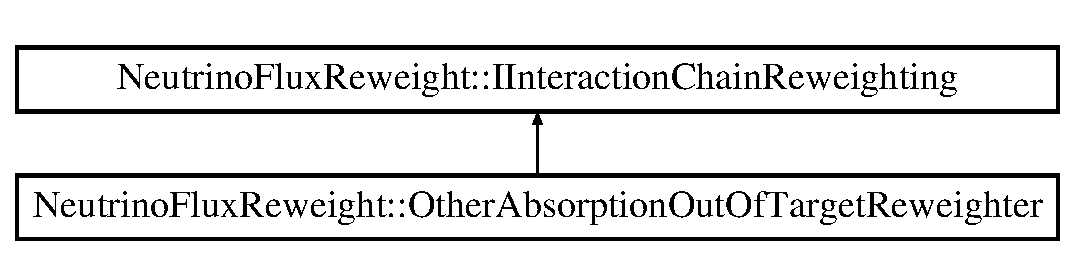
\includegraphics[height=2.000000cm]{class_neutrino_flux_reweight_1_1_other_absorption_out_of_target_reweighter}
\end{center}
\end{figure}
\subsection*{Public Member Functions}
\begin{DoxyCompactItemize}
\item 
\hyperlink{class_neutrino_flux_reweight_1_1_other_absorption_out_of_target_reweighter_affb154de07dd600158d0d7c0073ae9bb}{Other\-Absorption\-Out\-Of\-Target\-Reweighter} (int iuniv, const \hyperlink{class_neutrino_flux_reweight_1_1_parameter_table}{Parameter\-Table} \&cv\-\_\-pars, const \hyperlink{class_neutrino_flux_reweight_1_1_parameter_table}{Parameter\-Table} \&univ\-\_\-pars)
\item 
virtual \hyperlink{class_neutrino_flux_reweight_1_1_other_absorption_out_of_target_reweighter_a8830b6eb33389a9007b7b8b81f373f00}{$\sim$\-Other\-Absorption\-Out\-Of\-Target\-Reweighter} ()
\item 
virtual std\-::vector$<$ bool $>$ \hyperlink{class_neutrino_flux_reweight_1_1_other_absorption_out_of_target_reweighter_a5ab6da4e6a66b3ec9bcd24ddb4b90cb1}{can\-Reweight} (const \hyperlink{class_neutrino_flux_reweight_1_1_interaction_chain_data}{Interaction\-Chain\-Data} \&aa)
\begin{DoxyCompactList}\small\item\em Look through the \hyperlink{class_neutrino_flux_reweight_1_1_interaction_chain_data}{Interaction\-Chain\-Data} input and identify those Interactions that can be reweighted as part of a chain. We return a vector indicating which elements will be assigned a weight by calculate\-Weight. \end{DoxyCompactList}\item 
virtual double \hyperlink{class_neutrino_flux_reweight_1_1_other_absorption_out_of_target_reweighter_abebfe35083e25e8bca9eb0bf991d74d9}{calculate\-Weight} (const \hyperlink{class_neutrino_flux_reweight_1_1_interaction_chain_data}{Interaction\-Chain\-Data} \&aa)
\begin{DoxyCompactList}\small\item\em calculate a weight for this interaction chain given the central value parameters and the parameters for this universe. The weight is something like\-: f(cv)/f(M\-C) $\ast$ f(univ)/f(cv) where cv in this case corresponds to the best value of the parameter, given the data. If univ\-\_\-pars=cv\-\_\-pars then we are calculating a central value weight. Note, \hyperlink{class_neutrino_flux_reweight_1_1_other_absorption_out_of_target_reweighter_a5ab6da4e6a66b3ec9bcd24ddb4b90cb1}{can\-Reweight()} should be called to determine which elements of the chain are covered by the weight returned by \hyperlink{class_neutrino_flux_reweight_1_1_other_absorption_out_of_target_reweighter_abebfe35083e25e8bca9eb0bf991d74d9}{calculate\-Weight()} \end{DoxyCompactList}\end{DoxyCompactItemize}
\subsection*{Public Attributes}
\begin{DoxyCompactItemize}
\item 
const \hyperlink{class_neutrino_flux_reweight_1_1_parameter_table}{Parameter\-Table} \& \hyperlink{class_neutrino_flux_reweight_1_1_other_absorption_out_of_target_reweighter_a1fc316f75f145a3e388f48bbfe458e32}{cv\-Pars}
\item 
const \hyperlink{class_neutrino_flux_reweight_1_1_parameter_table}{Parameter\-Table} \& \hyperlink{class_neutrino_flux_reweight_1_1_other_absorption_out_of_target_reweighter_a02fc32769d87191294df9aaca580f529}{univ\-Pars}
\end{DoxyCompactItemize}
\subsection*{Private Attributes}
\begin{DoxyCompactItemize}
\item 
int \hyperlink{class_neutrino_flux_reweight_1_1_other_absorption_out_of_target_reweighter_aff30780c2efef88d0ef3d929ca8e9ae0}{i\-Univ}
\item 
float \hyperlink{class_neutrino_flux_reweight_1_1_other_absorption_out_of_target_reweighter_a1fa8ca53fe660fcc66886eb55d9db296}{inel\-\_\-kap\-Al\-\_\-xsec\-\_\-low\-P}
\item 
float \hyperlink{class_neutrino_flux_reweight_1_1_other_absorption_out_of_target_reweighter_a7fd78bf2576386f2854cca235f000e2a}{inel\-\_\-kap\-Al\-\_\-xsec\-\_\-high\-P}
\end{DoxyCompactItemize}


\subsection{Detailed Description}
Reweight a M\-C survival probabiity when the particles through volumes. 

Definition at line 16 of file Other\-Absorption\-Out\-Of\-Target\-Reweighter.\-h.



\subsection{Constructor \& Destructor Documentation}
\hypertarget{class_neutrino_flux_reweight_1_1_other_absorption_out_of_target_reweighter_affb154de07dd600158d0d7c0073ae9bb}{\index{Neutrino\-Flux\-Reweight\-::\-Other\-Absorption\-Out\-Of\-Target\-Reweighter@{Neutrino\-Flux\-Reweight\-::\-Other\-Absorption\-Out\-Of\-Target\-Reweighter}!Other\-Absorption\-Out\-Of\-Target\-Reweighter@{Other\-Absorption\-Out\-Of\-Target\-Reweighter}}
\index{Other\-Absorption\-Out\-Of\-Target\-Reweighter@{Other\-Absorption\-Out\-Of\-Target\-Reweighter}!NeutrinoFluxReweight::OtherAbsorptionOutOfTargetReweighter@{Neutrino\-Flux\-Reweight\-::\-Other\-Absorption\-Out\-Of\-Target\-Reweighter}}
\subsubsection[{Other\-Absorption\-Out\-Of\-Target\-Reweighter}]{\setlength{\rightskip}{0pt plus 5cm}Neutrino\-Flux\-Reweight\-::\-Other\-Absorption\-Out\-Of\-Target\-Reweighter\-::\-Other\-Absorption\-Out\-Of\-Target\-Reweighter (
\begin{DoxyParamCaption}
\item[{int}]{iuniv, }
\item[{const {\bf Parameter\-Table} \&}]{cv\-\_\-pars, }
\item[{const {\bf Parameter\-Table} \&}]{univ\-\_\-pars}
\end{DoxyParamCaption}
)}}\label{class_neutrino_flux_reweight_1_1_other_absorption_out_of_target_reweighter_affb154de07dd600158d0d7c0073ae9bb}
The constructor. Note, we pass central value and single universe parameters in this constructor only. There is thus a 1 to 1 correspondence between an instance of this class and a given universe. 

Definition at line 12 of file Other\-Absorption\-Out\-Of\-Target\-Reweighter.\-cpp.


\begin{DoxyCode}
12                                                                                                            
                                                :\hyperlink{class_neutrino_flux_reweight_1_1_other_absorption_out_of_target_reweighter_a1fc316f75f145a3e388f48bbfe458e32}{cvPars}(cv\_pars),\hyperlink{class_neutrino_flux_reweight_1_1_other_absorption_out_of_target_reweighter_a02fc32769d87191294df9aaca580f529}{univPars}(univ\_pars),
      \hyperlink{class_neutrino_flux_reweight_1_1_other_absorption_out_of_target_reweighter_aff30780c2efef88d0ef3d929ca8e9ae0}{iUniv}(iuniv)\{ 
13     
14     \textcolor{comment}{// const boost::interprocess::flat\_map<std::string, double>& dsig\_table = univPars.getMap();}
15     \hyperlink{class_neutrino_flux_reweight_1_1_other_absorption_out_of_target_reweighter_a1fa8ca53fe660fcc66886eb55d9db296}{inel\_kapAl\_xsec\_lowP}  = \hyperlink{class_neutrino_flux_reweight_1_1_other_absorption_out_of_target_reweighter_a02fc32769d87191294df9aaca580f529}{univPars}.
      \hyperlink{class_neutrino_flux_reweight_1_1_parameter_table_acb7dc8335b65b116f6092f2fa57ca5ed}{getParameterValue}(\textcolor{stringliteral}{"inel\_kapAl\_xsec\_lowP"});
16     \hyperlink{class_neutrino_flux_reweight_1_1_other_absorption_out_of_target_reweighter_a7fd78bf2576386f2854cca235f000e2a}{inel\_kapAl\_xsec\_highP} = \hyperlink{class_neutrino_flux_reweight_1_1_other_absorption_out_of_target_reweighter_a02fc32769d87191294df9aaca580f529}{univPars}.
      \hyperlink{class_neutrino_flux_reweight_1_1_parameter_table_acb7dc8335b65b116f6092f2fa57ca5ed}{getParameterValue}(\textcolor{stringliteral}{"inel\_kapAl\_xsec\_highP"});
17   \}
\end{DoxyCode}
\hypertarget{class_neutrino_flux_reweight_1_1_other_absorption_out_of_target_reweighter_a8830b6eb33389a9007b7b8b81f373f00}{\index{Neutrino\-Flux\-Reweight\-::\-Other\-Absorption\-Out\-Of\-Target\-Reweighter@{Neutrino\-Flux\-Reweight\-::\-Other\-Absorption\-Out\-Of\-Target\-Reweighter}!$\sim$\-Other\-Absorption\-Out\-Of\-Target\-Reweighter@{$\sim$\-Other\-Absorption\-Out\-Of\-Target\-Reweighter}}
\index{$\sim$\-Other\-Absorption\-Out\-Of\-Target\-Reweighter@{$\sim$\-Other\-Absorption\-Out\-Of\-Target\-Reweighter}!NeutrinoFluxReweight::OtherAbsorptionOutOfTargetReweighter@{Neutrino\-Flux\-Reweight\-::\-Other\-Absorption\-Out\-Of\-Target\-Reweighter}}
\subsubsection[{$\sim$\-Other\-Absorption\-Out\-Of\-Target\-Reweighter}]{\setlength{\rightskip}{0pt plus 5cm}Neutrino\-Flux\-Reweight\-::\-Other\-Absorption\-Out\-Of\-Target\-Reweighter\-::$\sim$\-Other\-Absorption\-Out\-Of\-Target\-Reweighter (
\begin{DoxyParamCaption}
{}
\end{DoxyParamCaption}
)\hspace{0.3cm}{\ttfamily [virtual]}}}\label{class_neutrino_flux_reweight_1_1_other_absorption_out_of_target_reweighter_a8830b6eb33389a9007b7b8b81f373f00}


Definition at line 18 of file Other\-Absorption\-Out\-Of\-Target\-Reweighter.\-cpp.


\begin{DoxyCode}
18                                                                              \{
19     
20   \}
\end{DoxyCode}


\subsection{Member Function Documentation}
\hypertarget{class_neutrino_flux_reweight_1_1_other_absorption_out_of_target_reweighter_abebfe35083e25e8bca9eb0bf991d74d9}{\index{Neutrino\-Flux\-Reweight\-::\-Other\-Absorption\-Out\-Of\-Target\-Reweighter@{Neutrino\-Flux\-Reweight\-::\-Other\-Absorption\-Out\-Of\-Target\-Reweighter}!calculate\-Weight@{calculate\-Weight}}
\index{calculate\-Weight@{calculate\-Weight}!NeutrinoFluxReweight::OtherAbsorptionOutOfTargetReweighter@{Neutrino\-Flux\-Reweight\-::\-Other\-Absorption\-Out\-Of\-Target\-Reweighter}}
\subsubsection[{calculate\-Weight}]{\setlength{\rightskip}{0pt plus 5cm}double Neutrino\-Flux\-Reweight\-::\-Other\-Absorption\-Out\-Of\-Target\-Reweighter\-::calculate\-Weight (
\begin{DoxyParamCaption}
\item[{const {\bf Interaction\-Chain\-Data} \&}]{aa}
\end{DoxyParamCaption}
)\hspace{0.3cm}{\ttfamily [virtual]}}}\label{class_neutrino_flux_reweight_1_1_other_absorption_out_of_target_reweighter_abebfe35083e25e8bca9eb0bf991d74d9}


calculate a weight for this interaction chain given the central value parameters and the parameters for this universe. The weight is something like\-: f(cv)/f(M\-C) $\ast$ f(univ)/f(cv) where cv in this case corresponds to the best value of the parameter, given the data. If univ\-\_\-pars=cv\-\_\-pars then we are calculating a central value weight. Note, \hyperlink{class_neutrino_flux_reweight_1_1_other_absorption_out_of_target_reweighter_a5ab6da4e6a66b3ec9bcd24ddb4b90cb1}{can\-Reweight()} should be called to determine which elements of the chain are covered by the weight returned by \hyperlink{class_neutrino_flux_reweight_1_1_other_absorption_out_of_target_reweighter_abebfe35083e25e8bca9eb0bf991d74d9}{calculate\-Weight()} 



Implements \hyperlink{class_neutrino_flux_reweight_1_1_i_interaction_chain_reweighting_ae28403553637013fdc720674ee24c7c5}{Neutrino\-Flux\-Reweight\-::\-I\-Interaction\-Chain\-Reweighting}.



Definition at line 41 of file Other\-Absorption\-Out\-Of\-Target\-Reweighter.\-cpp.


\begin{DoxyCode}
41                                                                                             \{
42     
43     std::vector<ParticlesThroughVolumesData>  vec\_ptv = aa.ptv\_info;
44 
45     \textcolor{keywordtype}{double} shift\_lowP = \hyperlink{class_neutrino_flux_reweight_1_1_other_absorption_out_of_target_reweighter_a1fa8ca53fe660fcc66886eb55d9db296}{inel\_kapAl\_xsec\_lowP};
46     \textcolor{keywordtype}{double} shift\_highP = \hyperlink{class_neutrino_flux_reweight_1_1_other_absorption_out_of_target_reweighter_a7fd78bf2576386f2854cca235f000e2a}{inel\_kapAl\_xsec\_highP};
47     
48     \textcolor{keywordtype}{double} NA\_mb    = 6.02E-4;
49     \textcolor{keywordtype}{double} wgt      = 1.0;
50     \textcolor{keywordtype}{double} tot\_dist = 0.0;
51     \textcolor{keywordtype}{double} low\_val  = 1.E-20;   
52     
53     \textcolor{keywordflow}{for}(\textcolor{keywordtype}{int} index\_vol=0;index\_vol<3;index\_vol++)\{
54       \textcolor{keywordflow}{for}(\textcolor{keywordtype}{int} ii=0;ii<3;ii++)\{
55         
56         tot\_dist = vec\_ptv[index\_vol].AmountMat[ii];
57         \textcolor{keywordflow}{if}(tot\_dist<low\_val)\textcolor{keywordflow}{continue};
58         \textcolor{keywordflow}{if}(abs(vec\_ptv[index\_vol].Pdgs[ii])==321 || abs(vec\_ptv[index\_vol].Pdgs[ii])==211 || vec\_ptv[
      index\_vol].Pdgs[ii]==2212 || vec\_ptv[index\_vol].Pdgs[ii]==2112 || abs(vec\_ptv[index\_vol].Pdgs[ii])<100)\textcolor{keywordflow}{continue};
59         
60         tot\_dist *= NA\_mb;
61         \textcolor{keywordflow}{if}(vec\_ptv[index\_vol].Moms[ii]<2.0)\{
62           tot\_dist *= shift\_lowP;
63         \}
64         \textcolor{keywordflow}{else} \textcolor{keywordflow}{if}(vec\_ptv[index\_vol].Moms[ii]>=2.0)\{
65           tot\_dist *= shift\_highP;
66         \}
67         wgt *= exp(-1.0*tot\_dist);   
68       \}
69     \}
70     \textcolor{keywordflow}{return} wgt;
71     
72   \}
\end{DoxyCode}
\hypertarget{class_neutrino_flux_reweight_1_1_other_absorption_out_of_target_reweighter_a5ab6da4e6a66b3ec9bcd24ddb4b90cb1}{\index{Neutrino\-Flux\-Reweight\-::\-Other\-Absorption\-Out\-Of\-Target\-Reweighter@{Neutrino\-Flux\-Reweight\-::\-Other\-Absorption\-Out\-Of\-Target\-Reweighter}!can\-Reweight@{can\-Reweight}}
\index{can\-Reweight@{can\-Reweight}!NeutrinoFluxReweight::OtherAbsorptionOutOfTargetReweighter@{Neutrino\-Flux\-Reweight\-::\-Other\-Absorption\-Out\-Of\-Target\-Reweighter}}
\subsubsection[{can\-Reweight}]{\setlength{\rightskip}{0pt plus 5cm}std\-::vector$<$ bool $>$ Neutrino\-Flux\-Reweight\-::\-Other\-Absorption\-Out\-Of\-Target\-Reweighter\-::can\-Reweight (
\begin{DoxyParamCaption}
\item[{const {\bf Interaction\-Chain\-Data} \&}]{aa}
\end{DoxyParamCaption}
)\hspace{0.3cm}{\ttfamily [virtual]}}}\label{class_neutrino_flux_reweight_1_1_other_absorption_out_of_target_reweighter_a5ab6da4e6a66b3ec9bcd24ddb4b90cb1}


Look through the \hyperlink{class_neutrino_flux_reweight_1_1_interaction_chain_data}{Interaction\-Chain\-Data} input and identify those Interactions that can be reweighted as part of a chain. We return a vector indicating which elements will be assigned a weight by calculate\-Weight. 



Implements \hyperlink{class_neutrino_flux_reweight_1_1_i_interaction_chain_reweighting_aacf17580c1d316f0ebcdfdff7418e9e3}{Neutrino\-Flux\-Reweight\-::\-I\-Interaction\-Chain\-Reweighting}.



Definition at line 21 of file Other\-Absorption\-Out\-Of\-Target\-Reweighter.\-cpp.


\begin{DoxyCode}
21                                                                                                  \{
22  
23     std::vector<bool> this\_nodes;
24     \textcolor{comment}{//int index\_vol = 0;}
25     \textcolor{keywordtype}{double} low\_val = 1.E-20;    
26   
27     std::vector<ParticlesThroughVolumesData>  vec\_ptv = aa.ptv\_info;
28 
29     \textcolor{keywordtype}{bool} passVOL = \textcolor{keyword}{false};
30     \textcolor{comment}{//Cheking at least one ancestor with amount of materail value:}
31     
32     \textcolor{keywordflow}{for}(\textcolor{keywordtype}{int} index\_vol=0;index\_vol<3;index\_vol++)\{
33       \textcolor{keywordflow}{for}(\textcolor{keywordtype}{int} ii=0;ii<3;ii++)\{
34         passVOL = passVOL || (vec\_ptv[index\_vol].AmountMat[ii] >low\_val && (abs(vec\_ptv[index\_vol].Pdgs[ii]
      )!=211 && abs(vec\_ptv[index\_vol].Pdgs[ii])!=321 && vec\_ptv[index\_vol].Pdgs[ii]!=2212 && vec\_ptv[index\_vol].
      Pdgs[ii]!=2112 && abs(vec\_ptv[index\_vol].Pdgs[ii])>99));
35       \}
36     \}
37     this\_nodes.push\_back(passVOL);
38     \textcolor{keywordflow}{return} this\_nodes;
39 
40   \}
\end{DoxyCode}


\subsection{Member Data Documentation}
\hypertarget{class_neutrino_flux_reweight_1_1_other_absorption_out_of_target_reweighter_a1fc316f75f145a3e388f48bbfe458e32}{\index{Neutrino\-Flux\-Reweight\-::\-Other\-Absorption\-Out\-Of\-Target\-Reweighter@{Neutrino\-Flux\-Reweight\-::\-Other\-Absorption\-Out\-Of\-Target\-Reweighter}!cv\-Pars@{cv\-Pars}}
\index{cv\-Pars@{cv\-Pars}!NeutrinoFluxReweight::OtherAbsorptionOutOfTargetReweighter@{Neutrino\-Flux\-Reweight\-::\-Other\-Absorption\-Out\-Of\-Target\-Reweighter}}
\subsubsection[{cv\-Pars}]{\setlength{\rightskip}{0pt plus 5cm}const {\bf Parameter\-Table}\& Neutrino\-Flux\-Reweight\-::\-Other\-Absorption\-Out\-Of\-Target\-Reweighter\-::cv\-Pars}}\label{class_neutrino_flux_reweight_1_1_other_absorption_out_of_target_reweighter_a1fc316f75f145a3e388f48bbfe458e32}


Definition at line 27 of file Other\-Absorption\-Out\-Of\-Target\-Reweighter.\-h.

\hypertarget{class_neutrino_flux_reweight_1_1_other_absorption_out_of_target_reweighter_a7fd78bf2576386f2854cca235f000e2a}{\index{Neutrino\-Flux\-Reweight\-::\-Other\-Absorption\-Out\-Of\-Target\-Reweighter@{Neutrino\-Flux\-Reweight\-::\-Other\-Absorption\-Out\-Of\-Target\-Reweighter}!inel\-\_\-kap\-Al\-\_\-xsec\-\_\-high\-P@{inel\-\_\-kap\-Al\-\_\-xsec\-\_\-high\-P}}
\index{inel\-\_\-kap\-Al\-\_\-xsec\-\_\-high\-P@{inel\-\_\-kap\-Al\-\_\-xsec\-\_\-high\-P}!NeutrinoFluxReweight::OtherAbsorptionOutOfTargetReweighter@{Neutrino\-Flux\-Reweight\-::\-Other\-Absorption\-Out\-Of\-Target\-Reweighter}}
\subsubsection[{inel\-\_\-kap\-Al\-\_\-xsec\-\_\-high\-P}]{\setlength{\rightskip}{0pt plus 5cm}float Neutrino\-Flux\-Reweight\-::\-Other\-Absorption\-Out\-Of\-Target\-Reweighter\-::inel\-\_\-kap\-Al\-\_\-xsec\-\_\-high\-P\hspace{0.3cm}{\ttfamily [private]}}}\label{class_neutrino_flux_reweight_1_1_other_absorption_out_of_target_reweighter_a7fd78bf2576386f2854cca235f000e2a}


Definition at line 31 of file Other\-Absorption\-Out\-Of\-Target\-Reweighter.\-h.

\hypertarget{class_neutrino_flux_reweight_1_1_other_absorption_out_of_target_reweighter_a1fa8ca53fe660fcc66886eb55d9db296}{\index{Neutrino\-Flux\-Reweight\-::\-Other\-Absorption\-Out\-Of\-Target\-Reweighter@{Neutrino\-Flux\-Reweight\-::\-Other\-Absorption\-Out\-Of\-Target\-Reweighter}!inel\-\_\-kap\-Al\-\_\-xsec\-\_\-low\-P@{inel\-\_\-kap\-Al\-\_\-xsec\-\_\-low\-P}}
\index{inel\-\_\-kap\-Al\-\_\-xsec\-\_\-low\-P@{inel\-\_\-kap\-Al\-\_\-xsec\-\_\-low\-P}!NeutrinoFluxReweight::OtherAbsorptionOutOfTargetReweighter@{Neutrino\-Flux\-Reweight\-::\-Other\-Absorption\-Out\-Of\-Target\-Reweighter}}
\subsubsection[{inel\-\_\-kap\-Al\-\_\-xsec\-\_\-low\-P}]{\setlength{\rightskip}{0pt plus 5cm}float Neutrino\-Flux\-Reweight\-::\-Other\-Absorption\-Out\-Of\-Target\-Reweighter\-::inel\-\_\-kap\-Al\-\_\-xsec\-\_\-low\-P\hspace{0.3cm}{\ttfamily [private]}}}\label{class_neutrino_flux_reweight_1_1_other_absorption_out_of_target_reweighter_a1fa8ca53fe660fcc66886eb55d9db296}


Definition at line 31 of file Other\-Absorption\-Out\-Of\-Target\-Reweighter.\-h.

\hypertarget{class_neutrino_flux_reweight_1_1_other_absorption_out_of_target_reweighter_aff30780c2efef88d0ef3d929ca8e9ae0}{\index{Neutrino\-Flux\-Reweight\-::\-Other\-Absorption\-Out\-Of\-Target\-Reweighter@{Neutrino\-Flux\-Reweight\-::\-Other\-Absorption\-Out\-Of\-Target\-Reweighter}!i\-Univ@{i\-Univ}}
\index{i\-Univ@{i\-Univ}!NeutrinoFluxReweight::OtherAbsorptionOutOfTargetReweighter@{Neutrino\-Flux\-Reweight\-::\-Other\-Absorption\-Out\-Of\-Target\-Reweighter}}
\subsubsection[{i\-Univ}]{\setlength{\rightskip}{0pt plus 5cm}int Neutrino\-Flux\-Reweight\-::\-Other\-Absorption\-Out\-Of\-Target\-Reweighter\-::i\-Univ\hspace{0.3cm}{\ttfamily [private]}}}\label{class_neutrino_flux_reweight_1_1_other_absorption_out_of_target_reweighter_aff30780c2efef88d0ef3d929ca8e9ae0}


Definition at line 30 of file Other\-Absorption\-Out\-Of\-Target\-Reweighter.\-h.

\hypertarget{class_neutrino_flux_reweight_1_1_other_absorption_out_of_target_reweighter_a02fc32769d87191294df9aaca580f529}{\index{Neutrino\-Flux\-Reweight\-::\-Other\-Absorption\-Out\-Of\-Target\-Reweighter@{Neutrino\-Flux\-Reweight\-::\-Other\-Absorption\-Out\-Of\-Target\-Reweighter}!univ\-Pars@{univ\-Pars}}
\index{univ\-Pars@{univ\-Pars}!NeutrinoFluxReweight::OtherAbsorptionOutOfTargetReweighter@{Neutrino\-Flux\-Reweight\-::\-Other\-Absorption\-Out\-Of\-Target\-Reweighter}}
\subsubsection[{univ\-Pars}]{\setlength{\rightskip}{0pt plus 5cm}const {\bf Parameter\-Table}\& Neutrino\-Flux\-Reweight\-::\-Other\-Absorption\-Out\-Of\-Target\-Reweighter\-::univ\-Pars}}\label{class_neutrino_flux_reweight_1_1_other_absorption_out_of_target_reweighter_a02fc32769d87191294df9aaca580f529}


Definition at line 28 of file Other\-Absorption\-Out\-Of\-Target\-Reweighter.\-h.



The documentation for this class was generated from the following files\-:\begin{DoxyCompactItemize}
\item 
include/\hyperlink{_other_absorption_out_of_target_reweighter_8h}{Other\-Absorption\-Out\-Of\-Target\-Reweighter.\-h}\item 
src/\hyperlink{_other_absorption_out_of_target_reweighter_8cpp}{Other\-Absorption\-Out\-Of\-Target\-Reweighter.\-cpp}\end{DoxyCompactItemize}

\hypertarget{class_neutrino_flux_reweight_1_1_other_reweighter}{\section{Neutrino\-Flux\-Reweight\-:\-:Other\-Reweighter Class Reference}
\label{class_neutrino_flux_reweight_1_1_other_reweighter}\index{Neutrino\-Flux\-Reweight\-::\-Other\-Reweighter@{Neutrino\-Flux\-Reweight\-::\-Other\-Reweighter}}
}


Reweighter of no thin target and no M\-I\-P\-P interactions.  




{\ttfamily \#include $<$Other\-Reweighter.\-h$>$}

Inheritance diagram for Neutrino\-Flux\-Reweight\-:\-:Other\-Reweighter\-:\begin{figure}[H]
\begin{center}
\leavevmode
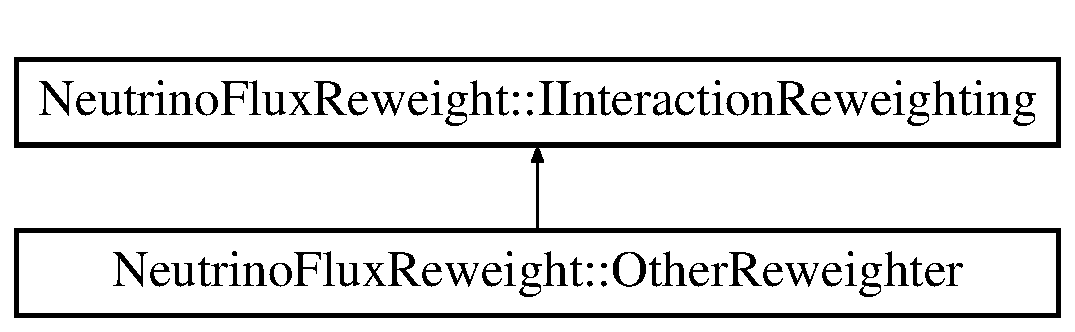
\includegraphics[height=2.000000cm]{class_neutrino_flux_reweight_1_1_other_reweighter}
\end{center}
\end{figure}
\subsection*{Public Member Functions}
\begin{DoxyCompactItemize}
\item 
\hyperlink{class_neutrino_flux_reweight_1_1_other_reweighter_a79bde0ab15d0b12ae67910708a464892}{Other\-Reweighter} (int iuniv, const \hyperlink{class_neutrino_flux_reweight_1_1_parameter_table}{Parameter\-Table} \&cv\-\_\-pars, const \hyperlink{class_neutrino_flux_reweight_1_1_parameter_table}{Parameter\-Table} \&univ\-\_\-pars)
\item 
virtual \hyperlink{class_neutrino_flux_reweight_1_1_other_reweighter_a001941f2120ae5832bb2086077038667}{$\sim$\-Other\-Reweighter} ()
\item 
virtual bool \hyperlink{class_neutrino_flux_reweight_1_1_other_reweighter_af5cadc4dcde8b9884962399b0a29bc5a}{can\-Reweight} (const \hyperlink{class_neutrino_flux_reweight_1_1_interaction_data}{Interaction\-Data} \&aa)
\begin{DoxyCompactList}\small\item\em can the particular instance of this class reweight this interaction? \end{DoxyCompactList}\item 
virtual double \hyperlink{class_neutrino_flux_reweight_1_1_other_reweighter_aca4a447053eede66a97747c98a2d89a2}{calculate\-Weight} (const \hyperlink{class_neutrino_flux_reweight_1_1_interaction_data}{Interaction\-Data} \&inter\-\_\-data)
\begin{DoxyCompactList}\small\item\em calculate a weight for this interaction given the central value parameters and the parameters for this universe. The weight is something like\-: f(cv)/f(M\-C) $\ast$ f(univ)/f(cv) where cv in this case corresponds to the best value of the parameter, given the data. If univ\-\_\-pars=cv\-\_\-pars then we are calculating a central value weight \end{DoxyCompactList}\end{DoxyCompactItemize}
\subsection*{Public Attributes}
\begin{DoxyCompactItemize}
\item 
const \hyperlink{class_neutrino_flux_reweight_1_1_parameter_table}{Parameter\-Table} \& \hyperlink{class_neutrino_flux_reweight_1_1_other_reweighter_a8dd49509293e302c005023668d153011}{cv\-Pars}
\item 
const \hyperlink{class_neutrino_flux_reweight_1_1_parameter_table}{Parameter\-Table} \& \hyperlink{class_neutrino_flux_reweight_1_1_other_reweighter_a2795ccb32eccdca967070a4768b9ca27}{univ\-Pars}
\end{DoxyCompactItemize}
\subsection*{Private Attributes}
\begin{DoxyCompactItemize}
\item 
int \hyperlink{class_neutrino_flux_reweight_1_1_other_reweighter_a8a778b0c554b88244ca4514c693d0e41}{i\-Univ}
\item 
float \hyperlink{class_neutrino_flux_reweight_1_1_other_reweighter_a8474c645b633b52935902771b36ac183}{inel\-\_\-\-A\-\_\-scaling}
\end{DoxyCompactItemize}


\subsection{Detailed Description}
Reweighter of no thin target and no M\-I\-P\-P interactions. 

Definition at line 19 of file Other\-Reweighter.\-h.



\subsection{Constructor \& Destructor Documentation}
\hypertarget{class_neutrino_flux_reweight_1_1_other_reweighter_a79bde0ab15d0b12ae67910708a464892}{\index{Neutrino\-Flux\-Reweight\-::\-Other\-Reweighter@{Neutrino\-Flux\-Reweight\-::\-Other\-Reweighter}!Other\-Reweighter@{Other\-Reweighter}}
\index{Other\-Reweighter@{Other\-Reweighter}!NeutrinoFluxReweight::OtherReweighter@{Neutrino\-Flux\-Reweight\-::\-Other\-Reweighter}}
\subsubsection[{Other\-Reweighter}]{\setlength{\rightskip}{0pt plus 5cm}Neutrino\-Flux\-Reweight\-::\-Other\-Reweighter\-::\-Other\-Reweighter (
\begin{DoxyParamCaption}
\item[{int}]{iuniv, }
\item[{const {\bf Parameter\-Table} \&}]{cv\-\_\-pars, }
\item[{const {\bf Parameter\-Table} \&}]{univ\-\_\-pars}
\end{DoxyParamCaption}
)}}\label{class_neutrino_flux_reweight_1_1_other_reweighter_a79bde0ab15d0b12ae67910708a464892}


Definition at line 7 of file Other\-Reweighter.\-cpp.


\begin{DoxyCode}
7                                                                                                            
      :\hyperlink{class_neutrino_flux_reweight_1_1_other_reweighter_a8dd49509293e302c005023668d153011}{cvPars}(cv\_pars),\hyperlink{class_neutrino_flux_reweight_1_1_other_reweighter_a2795ccb32eccdca967070a4768b9ca27}{univPars}(univ\_pars),\hyperlink{class_neutrino_flux_reweight_1_1_other_reweighter_a8a778b0c554b88244ca4514c693d0e41}{iUniv}(iuniv)\{
8     
9     \textcolor{comment}{// const boost::interprocess::flat\_map<std::string, double>& dsig\_table = univPars.getMap();}
10     \hyperlink{class_neutrino_flux_reweight_1_1_other_reweighter_a8474c645b633b52935902771b36ac183}{inel\_A\_scaling} = \hyperlink{class_neutrino_flux_reweight_1_1_other_reweighter_a2795ccb32eccdca967070a4768b9ca27}{univPars}.\hyperlink{class_neutrino_flux_reweight_1_1_parameter_table_acb7dc8335b65b116f6092f2fa57ca5ed}{getParameterValue}(\textcolor{stringliteral}{"inel\_A\_scaling"});
11     
12   \}
\end{DoxyCode}
\hypertarget{class_neutrino_flux_reweight_1_1_other_reweighter_a001941f2120ae5832bb2086077038667}{\index{Neutrino\-Flux\-Reweight\-::\-Other\-Reweighter@{Neutrino\-Flux\-Reweight\-::\-Other\-Reweighter}!$\sim$\-Other\-Reweighter@{$\sim$\-Other\-Reweighter}}
\index{$\sim$\-Other\-Reweighter@{$\sim$\-Other\-Reweighter}!NeutrinoFluxReweight::OtherReweighter@{Neutrino\-Flux\-Reweight\-::\-Other\-Reweighter}}
\subsubsection[{$\sim$\-Other\-Reweighter}]{\setlength{\rightskip}{0pt plus 5cm}Neutrino\-Flux\-Reweight\-::\-Other\-Reweighter\-::$\sim$\-Other\-Reweighter (
\begin{DoxyParamCaption}
{}
\end{DoxyParamCaption}
)\hspace{0.3cm}{\ttfamily [virtual]}}}\label{class_neutrino_flux_reweight_1_1_other_reweighter_a001941f2120ae5832bb2086077038667}


Definition at line 14 of file Other\-Reweighter.\-cpp.


\begin{DoxyCode}
14                                     \{
15     
16   \}
\end{DoxyCode}


\subsection{Member Function Documentation}
\hypertarget{class_neutrino_flux_reweight_1_1_other_reweighter_aca4a447053eede66a97747c98a2d89a2}{\index{Neutrino\-Flux\-Reweight\-::\-Other\-Reweighter@{Neutrino\-Flux\-Reweight\-::\-Other\-Reweighter}!calculate\-Weight@{calculate\-Weight}}
\index{calculate\-Weight@{calculate\-Weight}!NeutrinoFluxReweight::OtherReweighter@{Neutrino\-Flux\-Reweight\-::\-Other\-Reweighter}}
\subsubsection[{calculate\-Weight}]{\setlength{\rightskip}{0pt plus 5cm}double Neutrino\-Flux\-Reweight\-::\-Other\-Reweighter\-::calculate\-Weight (
\begin{DoxyParamCaption}
\item[{const {\bf Interaction\-Data} \&}]{inter\-\_\-data}
\end{DoxyParamCaption}
)\hspace{0.3cm}{\ttfamily [virtual]}}}\label{class_neutrino_flux_reweight_1_1_other_reweighter_aca4a447053eede66a97747c98a2d89a2}


calculate a weight for this interaction given the central value parameters and the parameters for this universe. The weight is something like\-: f(cv)/f(M\-C) $\ast$ f(univ)/f(cv) where cv in this case corresponds to the best value of the parameter, given the data. If univ\-\_\-pars=cv\-\_\-pars then we are calculating a central value weight 



Implements \hyperlink{class_neutrino_flux_reweight_1_1_i_interaction_reweighting_a49b0d73e778411d629205d23575703c3}{Neutrino\-Flux\-Reweight\-::\-I\-Interaction\-Reweighting}.



Definition at line 26 of file Other\-Reweighter.\-cpp.


\begin{DoxyCode}
26                                                                       \{
27     
28     \textcolor{keywordflow}{return} \hyperlink{class_neutrino_flux_reweight_1_1_other_reweighter_a8474c645b633b52935902771b36ac183}{inel\_A\_scaling};
29     
30   \}
\end{DoxyCode}
\hypertarget{class_neutrino_flux_reweight_1_1_other_reweighter_af5cadc4dcde8b9884962399b0a29bc5a}{\index{Neutrino\-Flux\-Reweight\-::\-Other\-Reweighter@{Neutrino\-Flux\-Reweight\-::\-Other\-Reweighter}!can\-Reweight@{can\-Reweight}}
\index{can\-Reweight@{can\-Reweight}!NeutrinoFluxReweight::OtherReweighter@{Neutrino\-Flux\-Reweight\-::\-Other\-Reweighter}}
\subsubsection[{can\-Reweight}]{\setlength{\rightskip}{0pt plus 5cm}bool Neutrino\-Flux\-Reweight\-::\-Other\-Reweighter\-::can\-Reweight (
\begin{DoxyParamCaption}
\item[{const {\bf Interaction\-Data} \&}]{aa}
\end{DoxyParamCaption}
)\hspace{0.3cm}{\ttfamily [virtual]}}}\label{class_neutrino_flux_reweight_1_1_other_reweighter_af5cadc4dcde8b9884962399b0a29bc5a}


can the particular instance of this class reweight this interaction? 



Implements \hyperlink{class_neutrino_flux_reweight_1_1_i_interaction_reweighting_aa3d1d3f37a93b02e447cf5eca333ac8d}{Neutrino\-Flux\-Reweight\-::\-I\-Interaction\-Reweighting}.



Definition at line 17 of file Other\-Reweighter.\-cpp.


\begin{DoxyCode}
17                                                             \{
18  
19     \textcolor{keywordflow}{if}(aa.Proc.find(\textcolor{stringliteral}{"Inelastic"})<100)\{
20       \textcolor{keywordflow}{return} \textcolor{keyword}{true};
21     \}
22     \textcolor{keywordflow}{else} \textcolor{keywordflow}{return} \textcolor{keyword}{false};
23     
24   \}
\end{DoxyCode}


\subsection{Member Data Documentation}
\hypertarget{class_neutrino_flux_reweight_1_1_other_reweighter_a8dd49509293e302c005023668d153011}{\index{Neutrino\-Flux\-Reweight\-::\-Other\-Reweighter@{Neutrino\-Flux\-Reweight\-::\-Other\-Reweighter}!cv\-Pars@{cv\-Pars}}
\index{cv\-Pars@{cv\-Pars}!NeutrinoFluxReweight::OtherReweighter@{Neutrino\-Flux\-Reweight\-::\-Other\-Reweighter}}
\subsubsection[{cv\-Pars}]{\setlength{\rightskip}{0pt plus 5cm}const {\bf Parameter\-Table}\& Neutrino\-Flux\-Reweight\-::\-Other\-Reweighter\-::cv\-Pars}}\label{class_neutrino_flux_reweight_1_1_other_reweighter_a8dd49509293e302c005023668d153011}


Definition at line 26 of file Other\-Reweighter.\-h.

\hypertarget{class_neutrino_flux_reweight_1_1_other_reweighter_a8474c645b633b52935902771b36ac183}{\index{Neutrino\-Flux\-Reweight\-::\-Other\-Reweighter@{Neutrino\-Flux\-Reweight\-::\-Other\-Reweighter}!inel\-\_\-\-A\-\_\-scaling@{inel\-\_\-\-A\-\_\-scaling}}
\index{inel\-\_\-\-A\-\_\-scaling@{inel\-\_\-\-A\-\_\-scaling}!NeutrinoFluxReweight::OtherReweighter@{Neutrino\-Flux\-Reweight\-::\-Other\-Reweighter}}
\subsubsection[{inel\-\_\-\-A\-\_\-scaling}]{\setlength{\rightskip}{0pt plus 5cm}float Neutrino\-Flux\-Reweight\-::\-Other\-Reweighter\-::inel\-\_\-\-A\-\_\-scaling\hspace{0.3cm}{\ttfamily [private]}}}\label{class_neutrino_flux_reweight_1_1_other_reweighter_a8474c645b633b52935902771b36ac183}


Definition at line 31 of file Other\-Reweighter.\-h.

\hypertarget{class_neutrino_flux_reweight_1_1_other_reweighter_a8a778b0c554b88244ca4514c693d0e41}{\index{Neutrino\-Flux\-Reweight\-::\-Other\-Reweighter@{Neutrino\-Flux\-Reweight\-::\-Other\-Reweighter}!i\-Univ@{i\-Univ}}
\index{i\-Univ@{i\-Univ}!NeutrinoFluxReweight::OtherReweighter@{Neutrino\-Flux\-Reweight\-::\-Other\-Reweighter}}
\subsubsection[{i\-Univ}]{\setlength{\rightskip}{0pt plus 5cm}int Neutrino\-Flux\-Reweight\-::\-Other\-Reweighter\-::i\-Univ\hspace{0.3cm}{\ttfamily [private]}}}\label{class_neutrino_flux_reweight_1_1_other_reweighter_a8a778b0c554b88244ca4514c693d0e41}


Definition at line 30 of file Other\-Reweighter.\-h.

\hypertarget{class_neutrino_flux_reweight_1_1_other_reweighter_a2795ccb32eccdca967070a4768b9ca27}{\index{Neutrino\-Flux\-Reweight\-::\-Other\-Reweighter@{Neutrino\-Flux\-Reweight\-::\-Other\-Reweighter}!univ\-Pars@{univ\-Pars}}
\index{univ\-Pars@{univ\-Pars}!NeutrinoFluxReweight::OtherReweighter@{Neutrino\-Flux\-Reweight\-::\-Other\-Reweighter}}
\subsubsection[{univ\-Pars}]{\setlength{\rightskip}{0pt plus 5cm}const {\bf Parameter\-Table}\& Neutrino\-Flux\-Reweight\-::\-Other\-Reweighter\-::univ\-Pars}}\label{class_neutrino_flux_reweight_1_1_other_reweighter_a2795ccb32eccdca967070a4768b9ca27}


Definition at line 27 of file Other\-Reweighter.\-h.



The documentation for this class was generated from the following files\-:\begin{DoxyCompactItemize}
\item 
include/\hyperlink{_other_reweighter_8h}{Other\-Reweighter.\-h}\item 
src/\hyperlink{_other_reweighter_8cpp}{Other\-Reweighter.\-cpp}\end{DoxyCompactItemize}

\hypertarget{class_neutrino_flux_reweight_1_1_parameter_table}{\section{Neutrino\-Flux\-Reweight\-:\-:Parameter\-Table Class Reference}
\label{class_neutrino_flux_reweight_1_1_parameter_table}\index{Neutrino\-Flux\-Reweight\-::\-Parameter\-Table@{Neutrino\-Flux\-Reweight\-::\-Parameter\-Table}}
}


A list/table of parameter names and values.  




{\ttfamily \#include $<$Parameter\-Table.\-h$>$}

\subsection*{Public Member Functions}
\begin{DoxyCompactItemize}
\item 
\hyperlink{class_neutrino_flux_reweight_1_1_parameter_table_ae86246f4fd43bf1c7b6f4b62ed6264e8}{Parameter\-Table} ()
\item 
void \hyperlink{class_neutrino_flux_reweight_1_1_parameter_table_a7523c0cc9f0e3f7e648b3d228eb69ec7}{set\-Parameter} (\hyperlink{namespace_neutrino_flux_reweight_aa1e1a244ea4addfb793b4e316e6c0a72}{Parameter} p)
\begin{DoxyCompactList}\small\item\em add a parameter to the table or, if already there, reset its value \end{DoxyCompactList}\item 
\hyperlink{namespace_neutrino_flux_reweight_aa1e1a244ea4addfb793b4e316e6c0a72}{Parameter} \hyperlink{class_neutrino_flux_reweight_1_1_parameter_table_ae8f523d62145ab49b3a84e689190332b}{get\-Parameter} (const std\-::string \&name) const 
\begin{DoxyCompactList}\small\item\em get a parameter by name. throw an exception of a well defined type if we don't have it \end{DoxyCompactList}\item 
double \hyperlink{class_neutrino_flux_reweight_1_1_parameter_table_acb7dc8335b65b116f6092f2fa57ca5ed}{get\-Parameter\-Value} (const std\-::string \&name) const 
\begin{DoxyCompactList}\small\item\em get the value of a parameter. throw an exception of a well defined type if we don't have it \end{DoxyCompactList}\item 
bool \hyperlink{class_neutrino_flux_reweight_1_1_parameter_table_a525c3a34a2468513b68e36c230a5e9fa}{has\-Parameter} (const std\-::string \&name) const 
\begin{DoxyCompactList}\small\item\em is the named parameter in the table? \end{DoxyCompactList}\item 
const \\*
boost\-::interprocess\-::flat\-\_\-map\\*
$<$ std\-::string, double $>$ \& \hyperlink{class_neutrino_flux_reweight_1_1_parameter_table_a5438f5f53449e8dc1a12dfff2b9d922f}{get\-Map} () const 
\end{DoxyCompactItemize}
\subsection*{Protected Member Functions}
\begin{DoxyCompactItemize}
\item 
void \hyperlink{class_neutrino_flux_reweight_1_1_parameter_table_a9f4b1dfd17971c027c20c54d9f0229f8}{mapify} () const 
\begin{DoxyCompactList}\small\item\em Move the parameters from the vector to the map. \end{DoxyCompactList}\end{DoxyCompactItemize}
\subsection*{Protected Attributes}
\begin{DoxyCompactItemize}
\item 
boost\-::interprocess\-::flat\-\_\-map\\*
$<$ std\-::string, double $>$ \hyperlink{class_neutrino_flux_reweight_1_1_parameter_table_a8568f2707a7541bc949d79d5961f429a}{table}
\item 
std\-::vector$<$ std\-::pair\\*
$<$ std\-::string, double $>$ $>$ \hyperlink{class_neutrino_flux_reweight_1_1_parameter_table_aea2a9552c84dae00ecdd95b6aa0a6f6c}{m\-\_\-vector}
\item 
bool \hyperlink{class_neutrino_flux_reweight_1_1_parameter_table_aaaeca6d7d1d1db64e3078effdca83a9c}{m\-\_\-vector\-Mode}
\end{DoxyCompactItemize}


\subsection{Detailed Description}
A list/table of parameter names and values. 

The memory overhead of std\-::map turns out to be large for our case, so we use a boost\-::flat\-\_\-map instead. This uses an ordered vector, so memory overhead is small. Insertion is slow, though, so we start out by putting all our parameters in a vector. At the first request for parameter or the entire map, we sort the vector, copy it into the map and free the vector. This is efficient when there is a \char`\"{}filling\char`\"{} phase when no reads are done, and a \char`\"{}reading\char`\"{} phase, when no more fills are done. 

Definition at line 30 of file Parameter\-Table.\-h.



\subsection{Constructor \& Destructor Documentation}
\hypertarget{class_neutrino_flux_reweight_1_1_parameter_table_ae86246f4fd43bf1c7b6f4b62ed6264e8}{\index{Neutrino\-Flux\-Reweight\-::\-Parameter\-Table@{Neutrino\-Flux\-Reweight\-::\-Parameter\-Table}!Parameter\-Table@{Parameter\-Table}}
\index{Parameter\-Table@{Parameter\-Table}!NeutrinoFluxReweight::ParameterTable@{Neutrino\-Flux\-Reweight\-::\-Parameter\-Table}}
\subsubsection[{Parameter\-Table}]{\setlength{\rightskip}{0pt plus 5cm}Neutrino\-Flux\-Reweight\-::\-Parameter\-Table\-::\-Parameter\-Table (
\begin{DoxyParamCaption}
{}
\end{DoxyParamCaption}
)\hspace{0.3cm}{\ttfamily [inline]}}}\label{class_neutrino_flux_reweight_1_1_parameter_table_ae86246f4fd43bf1c7b6f4b62ed6264e8}


Definition at line 32 of file Parameter\-Table.\-h.


\begin{DoxyCode}
33       : \hyperlink{class_neutrino_flux_reweight_1_1_parameter_table_aaaeca6d7d1d1db64e3078effdca83a9c}{m\_vectorMode}(\textcolor{keyword}{true})
34       \{\}
\end{DoxyCode}


\subsection{Member Function Documentation}
\hypertarget{class_neutrino_flux_reweight_1_1_parameter_table_a5438f5f53449e8dc1a12dfff2b9d922f}{\index{Neutrino\-Flux\-Reweight\-::\-Parameter\-Table@{Neutrino\-Flux\-Reweight\-::\-Parameter\-Table}!get\-Map@{get\-Map}}
\index{get\-Map@{get\-Map}!NeutrinoFluxReweight::ParameterTable@{Neutrino\-Flux\-Reweight\-::\-Parameter\-Table}}
\subsubsection[{get\-Map}]{\setlength{\rightskip}{0pt plus 5cm}const boost\-::interprocess\-::flat\-\_\-map$<$std\-::string, double$>$\& Neutrino\-Flux\-Reweight\-::\-Parameter\-Table\-::get\-Map (
\begin{DoxyParamCaption}
{}
\end{DoxyParamCaption}
) const\hspace{0.3cm}{\ttfamily [inline]}}}\label{class_neutrino_flux_reweight_1_1_parameter_table_a5438f5f53449e8dc1a12dfff2b9d922f}


Definition at line 45 of file Parameter\-Table.\-h.


\begin{DoxyCode}
45 \{ \hyperlink{class_neutrino_flux_reweight_1_1_parameter_table_a9f4b1dfd17971c027c20c54d9f0229f8}{mapify}(); \textcolor{keywordflow}{return} \hyperlink{class_neutrino_flux_reweight_1_1_parameter_table_a8568f2707a7541bc949d79d5961f429a}{table}; \}
\end{DoxyCode}
\hypertarget{class_neutrino_flux_reweight_1_1_parameter_table_ae8f523d62145ab49b3a84e689190332b}{\index{Neutrino\-Flux\-Reweight\-::\-Parameter\-Table@{Neutrino\-Flux\-Reweight\-::\-Parameter\-Table}!get\-Parameter@{get\-Parameter}}
\index{get\-Parameter@{get\-Parameter}!NeutrinoFluxReweight::ParameterTable@{Neutrino\-Flux\-Reweight\-::\-Parameter\-Table}}
\subsubsection[{get\-Parameter}]{\setlength{\rightskip}{0pt plus 5cm}{\bf Parameter} Neutrino\-Flux\-Reweight\-::\-Parameter\-Table\-::get\-Parameter (
\begin{DoxyParamCaption}
\item[{const std\-::string \&}]{name}
\end{DoxyParamCaption}
) const}}\label{class_neutrino_flux_reweight_1_1_parameter_table_ae8f523d62145ab49b3a84e689190332b}


get a parameter by name. throw an exception of a well defined type if we don't have it 



Definition at line 17 of file Parameter\-Table.\-cpp.


\begin{DoxyCode}
17                                                                     \{
18     \hyperlink{class_neutrino_flux_reweight_1_1_parameter_table_a9f4b1dfd17971c027c20c54d9f0229f8}{mapify}();
19     \hyperlink{namespace_neutrino_flux_reweight_aa1e1a244ea4addfb793b4e316e6c0a72}{Parameter} pOut;
20     boost::interprocess::flat\_map<std::string, double>::const\_iterator it=\hyperlink{class_neutrino_flux_reweight_1_1_parameter_table_a8568f2707a7541bc949d79d5961f429a}{table}.find(name);
21     
22     \textcolor{keywordflow}{if}(it!=\hyperlink{class_neutrino_flux_reweight_1_1_parameter_table_a8568f2707a7541bc949d79d5961f429a}{table}.end())\{
23       pOut.first  = name;
24       pOut.second = it->second;
25     \}
26     \textcolor{keywordflow}{else}\{
27       \textcolor{keywordflow}{throw} \hyperlink{struct_no_parameter_found}{NoParameterFound}(name);
28     \}
29     \textcolor{keywordflow}{return} pOut;
30     
31   \}
\end{DoxyCode}
\hypertarget{class_neutrino_flux_reweight_1_1_parameter_table_acb7dc8335b65b116f6092f2fa57ca5ed}{\index{Neutrino\-Flux\-Reweight\-::\-Parameter\-Table@{Neutrino\-Flux\-Reweight\-::\-Parameter\-Table}!get\-Parameter\-Value@{get\-Parameter\-Value}}
\index{get\-Parameter\-Value@{get\-Parameter\-Value}!NeutrinoFluxReweight::ParameterTable@{Neutrino\-Flux\-Reweight\-::\-Parameter\-Table}}
\subsubsection[{get\-Parameter\-Value}]{\setlength{\rightskip}{0pt plus 5cm}double Neutrino\-Flux\-Reweight\-::\-Parameter\-Table\-::get\-Parameter\-Value (
\begin{DoxyParamCaption}
\item[{const std\-::string \&}]{name}
\end{DoxyParamCaption}
) const}}\label{class_neutrino_flux_reweight_1_1_parameter_table_acb7dc8335b65b116f6092f2fa57ca5ed}


get the value of a parameter. throw an exception of a well defined type if we don't have it 



Definition at line 33 of file Parameter\-Table.\-cpp.


\begin{DoxyCode}
33                                                                       \{
34     \hyperlink{class_neutrino_flux_reweight_1_1_parameter_table_a9f4b1dfd17971c027c20c54d9f0229f8}{mapify}();
35 
36     \textcolor{keywordtype}{double} val;
37     boost::interprocess::flat\_map<std::string, double>::const\_iterator it=\hyperlink{class_neutrino_flux_reweight_1_1_parameter_table_a8568f2707a7541bc949d79d5961f429a}{table}.find(name);
38     
39     \textcolor{keywordflow}{if}(it!=\hyperlink{class_neutrino_flux_reweight_1_1_parameter_table_a8568f2707a7541bc949d79d5961f429a}{table}.end())\{
40       val = it->second;
41     \}
42     \textcolor{keywordflow}{else}\{
43       \textcolor{keywordflow}{throw} \hyperlink{struct_no_parameter_found}{NoParameterFound}(name);
44     \}
45     
46     \textcolor{keywordflow}{return} val;
47     
48   \}
\end{DoxyCode}
\hypertarget{class_neutrino_flux_reweight_1_1_parameter_table_a525c3a34a2468513b68e36c230a5e9fa}{\index{Neutrino\-Flux\-Reweight\-::\-Parameter\-Table@{Neutrino\-Flux\-Reweight\-::\-Parameter\-Table}!has\-Parameter@{has\-Parameter}}
\index{has\-Parameter@{has\-Parameter}!NeutrinoFluxReweight::ParameterTable@{Neutrino\-Flux\-Reweight\-::\-Parameter\-Table}}
\subsubsection[{has\-Parameter}]{\setlength{\rightskip}{0pt plus 5cm}bool Neutrino\-Flux\-Reweight\-::\-Parameter\-Table\-::has\-Parameter (
\begin{DoxyParamCaption}
\item[{const std\-::string \&}]{name}
\end{DoxyParamCaption}
) const}}\label{class_neutrino_flux_reweight_1_1_parameter_table_a525c3a34a2468513b68e36c230a5e9fa}


is the named parameter in the table? 



Definition at line 50 of file Parameter\-Table.\-cpp.


\begin{DoxyCode}
50                                                                \{
51     \hyperlink{class_neutrino_flux_reweight_1_1_parameter_table_a9f4b1dfd17971c027c20c54d9f0229f8}{mapify}();
52     \textcolor{keywordflow}{return} \hyperlink{class_neutrino_flux_reweight_1_1_parameter_table_a8568f2707a7541bc949d79d5961f429a}{table}.find(name)!=\hyperlink{class_neutrino_flux_reweight_1_1_parameter_table_a8568f2707a7541bc949d79d5961f429a}{table}.end();
53   \}  
\end{DoxyCode}
\hypertarget{class_neutrino_flux_reweight_1_1_parameter_table_a9f4b1dfd17971c027c20c54d9f0229f8}{\index{Neutrino\-Flux\-Reweight\-::\-Parameter\-Table@{Neutrino\-Flux\-Reweight\-::\-Parameter\-Table}!mapify@{mapify}}
\index{mapify@{mapify}!NeutrinoFluxReweight::ParameterTable@{Neutrino\-Flux\-Reweight\-::\-Parameter\-Table}}
\subsubsection[{mapify}]{\setlength{\rightskip}{0pt plus 5cm}void Neutrino\-Flux\-Reweight\-::\-Parameter\-Table\-::mapify (
\begin{DoxyParamCaption}
{}
\end{DoxyParamCaption}
) const\hspace{0.3cm}{\ttfamily [protected]}}}\label{class_neutrino_flux_reweight_1_1_parameter_table_a9f4b1dfd17971c027c20c54d9f0229f8}


Move the parameters from the vector to the map. 



Definition at line 55 of file Parameter\-Table.\-cpp.


\begin{DoxyCode}
56   \{
57     \textcolor{comment}{// If we're already out of vector mode, there's nothing to do}
58     \textcolor{keywordflow}{if}(!\hyperlink{class_neutrino_flux_reweight_1_1_parameter_table_aaaeca6d7d1d1db64e3078effdca83a9c}{m\_vectorMode}) \textcolor{keywordflow}{return};
59 
60     \textcolor{comment}{// Sort the vector, populate the flat\_map from it, and then clear}
61     \textcolor{comment}{// the vector}
62     std::sort(\hyperlink{class_neutrino_flux_reweight_1_1_parameter_table_aea2a9552c84dae00ecdd95b6aa0a6f6c}{m\_vector}.begin(), \hyperlink{class_neutrino_flux_reweight_1_1_parameter_table_aea2a9552c84dae00ecdd95b6aa0a6f6c}{m\_vector}.end());
63     \hyperlink{class_neutrino_flux_reweight_1_1_parameter_table_a8568f2707a7541bc949d79d5961f429a}{table}=boost::interprocess::flat\_map<std::string, double>(\hyperlink{class_neutrino_flux_reweight_1_1_parameter_table_aea2a9552c84dae00ecdd95b6aa0a6f6c}{m\_vector}.begin(), 
      \hyperlink{class_neutrino_flux_reweight_1_1_parameter_table_aea2a9552c84dae00ecdd95b6aa0a6f6c}{m\_vector}.end());
64     \hyperlink{class_neutrino_flux_reweight_1_1_parameter_table_aea2a9552c84dae00ecdd95b6aa0a6f6c}{m\_vector}.clear();
65     \textcolor{comment}{// Magic to force the memory to be released: clear() doesn't do that}
66     std::vector<std::pair<std::string, double> >().swap(\hyperlink{class_neutrino_flux_reweight_1_1_parameter_table_aea2a9552c84dae00ecdd95b6aa0a6f6c}{m\_vector});
67     \textcolor{comment}{// We're no longer in vector mode, so we won't run this function}
68     \textcolor{comment}{// again}
69     \hyperlink{class_neutrino_flux_reweight_1_1_parameter_table_aaaeca6d7d1d1db64e3078effdca83a9c}{m\_vectorMode}=\textcolor{keyword}{false};
70   \}
\end{DoxyCode}
\hypertarget{class_neutrino_flux_reweight_1_1_parameter_table_a7523c0cc9f0e3f7e648b3d228eb69ec7}{\index{Neutrino\-Flux\-Reweight\-::\-Parameter\-Table@{Neutrino\-Flux\-Reweight\-::\-Parameter\-Table}!set\-Parameter@{set\-Parameter}}
\index{set\-Parameter@{set\-Parameter}!NeutrinoFluxReweight::ParameterTable@{Neutrino\-Flux\-Reweight\-::\-Parameter\-Table}}
\subsubsection[{set\-Parameter}]{\setlength{\rightskip}{0pt plus 5cm}void Neutrino\-Flux\-Reweight\-::\-Parameter\-Table\-::set\-Parameter (
\begin{DoxyParamCaption}
\item[{{\bf Parameter}}]{p}
\end{DoxyParamCaption}
)}}\label{class_neutrino_flux_reweight_1_1_parameter_table_a7523c0cc9f0e3f7e648b3d228eb69ec7}


add a parameter to the table or, if already there, reset its value 



Definition at line 8 of file Parameter\-Table.\-cpp.


\begin{DoxyCode}
8                                               \{
9     \textcolor{keywordflow}{if}(\hyperlink{class_neutrino_flux_reweight_1_1_parameter_table_aaaeca6d7d1d1db64e3078effdca83a9c}{m\_vectorMode})\{
10       \hyperlink{class_neutrino_flux_reweight_1_1_parameter_table_aea2a9552c84dae00ecdd95b6aa0a6f6c}{m\_vector}.push\_back(p);
11     \}
12     \textcolor{keywordflow}{else}\{
13       \hyperlink{class_neutrino_flux_reweight_1_1_parameter_table_a8568f2707a7541bc949d79d5961f429a}{table}[p.first] = p.second;
14     \}
15   \}
\end{DoxyCode}


\subsection{Member Data Documentation}
\hypertarget{class_neutrino_flux_reweight_1_1_parameter_table_aea2a9552c84dae00ecdd95b6aa0a6f6c}{\index{Neutrino\-Flux\-Reweight\-::\-Parameter\-Table@{Neutrino\-Flux\-Reweight\-::\-Parameter\-Table}!m\-\_\-vector@{m\-\_\-vector}}
\index{m\-\_\-vector@{m\-\_\-vector}!NeutrinoFluxReweight::ParameterTable@{Neutrino\-Flux\-Reweight\-::\-Parameter\-Table}}
\subsubsection[{m\-\_\-vector}]{\setlength{\rightskip}{0pt plus 5cm}std\-::vector$<$std\-::pair$<$std\-::string, double$>$ $>$ Neutrino\-Flux\-Reweight\-::\-Parameter\-Table\-::m\-\_\-vector\hspace{0.3cm}{\ttfamily [mutable]}, {\ttfamily [protected]}}}\label{class_neutrino_flux_reweight_1_1_parameter_table_aea2a9552c84dae00ecdd95b6aa0a6f6c}


Definition at line 51 of file Parameter\-Table.\-h.

\hypertarget{class_neutrino_flux_reweight_1_1_parameter_table_aaaeca6d7d1d1db64e3078effdca83a9c}{\index{Neutrino\-Flux\-Reweight\-::\-Parameter\-Table@{Neutrino\-Flux\-Reweight\-::\-Parameter\-Table}!m\-\_\-vector\-Mode@{m\-\_\-vector\-Mode}}
\index{m\-\_\-vector\-Mode@{m\-\_\-vector\-Mode}!NeutrinoFluxReweight::ParameterTable@{Neutrino\-Flux\-Reweight\-::\-Parameter\-Table}}
\subsubsection[{m\-\_\-vector\-Mode}]{\setlength{\rightskip}{0pt plus 5cm}bool Neutrino\-Flux\-Reweight\-::\-Parameter\-Table\-::m\-\_\-vector\-Mode\hspace{0.3cm}{\ttfamily [mutable]}, {\ttfamily [protected]}}}\label{class_neutrino_flux_reweight_1_1_parameter_table_aaaeca6d7d1d1db64e3078effdca83a9c}


Definition at line 52 of file Parameter\-Table.\-h.

\hypertarget{class_neutrino_flux_reweight_1_1_parameter_table_a8568f2707a7541bc949d79d5961f429a}{\index{Neutrino\-Flux\-Reweight\-::\-Parameter\-Table@{Neutrino\-Flux\-Reweight\-::\-Parameter\-Table}!table@{table}}
\index{table@{table}!NeutrinoFluxReweight::ParameterTable@{Neutrino\-Flux\-Reweight\-::\-Parameter\-Table}}
\subsubsection[{table}]{\setlength{\rightskip}{0pt plus 5cm}boost\-::interprocess\-::flat\-\_\-map$<$std\-::string, double$>$ Neutrino\-Flux\-Reweight\-::\-Parameter\-Table\-::table\hspace{0.3cm}{\ttfamily [mutable]}, {\ttfamily [protected]}}}\label{class_neutrino_flux_reweight_1_1_parameter_table_a8568f2707a7541bc949d79d5961f429a}


Definition at line 50 of file Parameter\-Table.\-h.



The documentation for this class was generated from the following files\-:\begin{DoxyCompactItemize}
\item 
include/\hyperlink{_parameter_table_8h}{Parameter\-Table.\-h}\item 
src/\hyperlink{_parameter_table_8cpp}{Parameter\-Table.\-cpp}\end{DoxyCompactItemize}

\hypertarget{class_particles_through_volumes}{\section{Particles\-Through\-Volumes Class Reference}
\label{class_particles_through_volumes}\index{Particles\-Through\-Volumes@{Particles\-Through\-Volumes}}
}


The information about the distance (multiplied by the density) of the particles passed by a volume.  




{\ttfamily \#include $<$Particles\-Through\-Volumes\-Data.\-h$>$}



\subsection{Detailed Description}
The information about the distance (multiplied by the density) of the particles passed by a volume. 

The documentation for this class was generated from the following file\-:\begin{DoxyCompactItemize}
\item 
include/\hyperlink{_particles_through_volumes_data_8h}{Particles\-Through\-Volumes\-Data.\-h}\end{DoxyCompactItemize}

\hypertarget{class_neutrino_flux_reweight_1_1_particles_through_volumes_data}{\section{Neutrino\-Flux\-Reweight\-:\-:Particles\-Through\-Volumes\-Data Class Reference}
\label{class_neutrino_flux_reweight_1_1_particles_through_volumes_data}\index{Neutrino\-Flux\-Reweight\-::\-Particles\-Through\-Volumes\-Data@{Neutrino\-Flux\-Reweight\-::\-Particles\-Through\-Volumes\-Data}}
}


{\ttfamily \#include $<$Particles\-Through\-Volumes\-Data.\-h$>$}

\subsection*{Public Member Functions}
\begin{DoxyCompactItemize}
\item 
\hyperlink{class_neutrino_flux_reweight_1_1_particles_through_volumes_data_a76d9b63fcd7df6dd58cc2930c97c30d6}{Particles\-Through\-Volumes\-Data} ()
\begin{DoxyCompactList}\small\item\em Default Constructor. \end{DoxyCompactList}\item 
\hyperlink{class_neutrino_flux_reweight_1_1_particles_through_volumes_data_a88d723bd3f60814f60ca1e662cb61273}{Particles\-Through\-Volumes\-Data} (int ptv\-\_\-pdg\mbox{[}$\,$\mbox{]}, double ptv\-\_\-amount\-\_\-mat\mbox{[}$\,$\mbox{]}, double ptv\-\_\-mom\mbox{[}$\,$\mbox{]}, std\-::string ptv\-\_\-vol)
\begin{DoxyCompactList}\small\item\em Constructor given the kinematic and distance traveled in the volume. \end{DoxyCompactList}\item 
virtual \hyperlink{class_neutrino_flux_reweight_1_1_particles_through_volumes_data_a75fff6e7df3509b1a2e15a53581ae027}{$\sim$\-Particles\-Through\-Volumes\-Data} ()
\item 
std\-::ostream \& \hyperlink{class_neutrino_flux_reweight_1_1_particles_through_volumes_data_a61a5d6880ad08ae17b6b47b645368f00}{print} (std\-::ostream \&os) const 
\end{DoxyCompactItemize}
\subsection*{Public Attributes}
\begin{DoxyCompactItemize}
\item 
int \hyperlink{class_neutrino_flux_reweight_1_1_particles_through_volumes_data_aa4f638f9eebba5ba2d59f909c077fa19}{Pdgs} \mbox{[}3\mbox{]}
\begin{DoxyCompactList}\small\item\em pdg codes of the particles \end{DoxyCompactList}\item 
double \hyperlink{class_neutrino_flux_reweight_1_1_particles_through_volumes_data_a897eba4f8766a1c110c4e473150f6c6e}{Amount\-Mat} \mbox{[}3\mbox{]}
\begin{DoxyCompactList}\small\item\em distance multiplied by volume \end{DoxyCompactList}\item 
double \hyperlink{class_neutrino_flux_reweight_1_1_particles_through_volumes_data_a373e722f967c878fa1749ae224a721fc}{Moms} \mbox{[}3\mbox{]}
\begin{DoxyCompactList}\small\item\em Momentum of the particles. \end{DoxyCompactList}\item 
std\-::string \hyperlink{class_neutrino_flux_reweight_1_1_particles_through_volumes_data_a7981341eb993e13d4512cf438c1c2e52}{Vol}
\begin{DoxyCompactList}\small\item\em Voulme. \end{DoxyCompactList}\end{DoxyCompactItemize}


\subsection{Detailed Description}


Definition at line 12 of file Particles\-Through\-Volumes\-Data.\-h.



\subsection{Constructor \& Destructor Documentation}
\hypertarget{class_neutrino_flux_reweight_1_1_particles_through_volumes_data_a76d9b63fcd7df6dd58cc2930c97c30d6}{\index{Neutrino\-Flux\-Reweight\-::\-Particles\-Through\-Volumes\-Data@{Neutrino\-Flux\-Reweight\-::\-Particles\-Through\-Volumes\-Data}!Particles\-Through\-Volumes\-Data@{Particles\-Through\-Volumes\-Data}}
\index{Particles\-Through\-Volumes\-Data@{Particles\-Through\-Volumes\-Data}!NeutrinoFluxReweight::ParticlesThroughVolumesData@{Neutrino\-Flux\-Reweight\-::\-Particles\-Through\-Volumes\-Data}}
\subsubsection[{Particles\-Through\-Volumes\-Data}]{\setlength{\rightskip}{0pt plus 5cm}Neutrino\-Flux\-Reweight\-::\-Particles\-Through\-Volumes\-Data\-::\-Particles\-Through\-Volumes\-Data (
\begin{DoxyParamCaption}
{}
\end{DoxyParamCaption}
)}}\label{class_neutrino_flux_reweight_1_1_particles_through_volumes_data_a76d9b63fcd7df6dd58cc2930c97c30d6}


Default Constructor. 

default values\-: 

Definition at line 7 of file Particles\-Through\-Volumes\-Data.\-cpp.


\begin{DoxyCode}
7                                                           \{
8    \textcolor{comment}{}
9 \textcolor{comment}{    //!default values: }
10 \textcolor{comment}{}    \hyperlink{class_neutrino_flux_reweight_1_1_particles_through_volumes_data_aa4f638f9eebba5ba2d59f909c077fa19}{Pdgs}[0] = 0;
11     \hyperlink{class_neutrino_flux_reweight_1_1_particles_through_volumes_data_aa4f638f9eebba5ba2d59f909c077fa19}{Pdgs}[1] = 0;
12     \hyperlink{class_neutrino_flux_reweight_1_1_particles_through_volumes_data_aa4f638f9eebba5ba2d59f909c077fa19}{Pdgs}[2] = 0;
13     
14     \hyperlink{class_neutrino_flux_reweight_1_1_particles_through_volumes_data_a897eba4f8766a1c110c4e473150f6c6e}{AmountMat}[0] = -1.0;
15     \hyperlink{class_neutrino_flux_reweight_1_1_particles_through_volumes_data_a897eba4f8766a1c110c4e473150f6c6e}{AmountMat}[1] = -1.0;
16     \hyperlink{class_neutrino_flux_reweight_1_1_particles_through_volumes_data_a897eba4f8766a1c110c4e473150f6c6e}{AmountMat}[2] = -1.0;
17 
18     \hyperlink{class_neutrino_flux_reweight_1_1_particles_through_volumes_data_a373e722f967c878fa1749ae224a721fc}{Moms}[0] = 0.0;
19     \hyperlink{class_neutrino_flux_reweight_1_1_particles_through_volumes_data_a373e722f967c878fa1749ae224a721fc}{Moms}[1] = 0.0;
20     \hyperlink{class_neutrino_flux_reweight_1_1_particles_through_volumes_data_a373e722f967c878fa1749ae224a721fc}{Moms}[2] = 0.0;
21     
22     \hyperlink{class_neutrino_flux_reweight_1_1_particles_through_volumes_data_a7981341eb993e13d4512cf438c1c2e52}{Vol} = \textcolor{stringliteral}{"None"};
23   \}
\end{DoxyCode}
\hypertarget{class_neutrino_flux_reweight_1_1_particles_through_volumes_data_a88d723bd3f60814f60ca1e662cb61273}{\index{Neutrino\-Flux\-Reweight\-::\-Particles\-Through\-Volumes\-Data@{Neutrino\-Flux\-Reweight\-::\-Particles\-Through\-Volumes\-Data}!Particles\-Through\-Volumes\-Data@{Particles\-Through\-Volumes\-Data}}
\index{Particles\-Through\-Volumes\-Data@{Particles\-Through\-Volumes\-Data}!NeutrinoFluxReweight::ParticlesThroughVolumesData@{Neutrino\-Flux\-Reweight\-::\-Particles\-Through\-Volumes\-Data}}
\subsubsection[{Particles\-Through\-Volumes\-Data}]{\setlength{\rightskip}{0pt plus 5cm}Neutrino\-Flux\-Reweight\-::\-Particles\-Through\-Volumes\-Data\-::\-Particles\-Through\-Volumes\-Data (
\begin{DoxyParamCaption}
\item[{int}]{ptv\-\_\-pdg\mbox{[}$\,$\mbox{]}, }
\item[{double}]{ptv\-\_\-amount\-\_\-mat\mbox{[}$\,$\mbox{]}, }
\item[{double}]{ptv\-\_\-mom\mbox{[}$\,$\mbox{]}, }
\item[{std\-::string}]{ptv\-\_\-vol}
\end{DoxyParamCaption}
)}}\label{class_neutrino_flux_reweight_1_1_particles_through_volumes_data_a88d723bd3f60814f60ca1e662cb61273}


Constructor given the kinematic and distance traveled in the volume. 

I assumed arrays of dimmension 3\-: 

Definition at line 25 of file Particles\-Through\-Volumes\-Data.\-cpp.


\begin{DoxyCode}
25                                                                                                            
                               \{
26 \textcolor{comment}{}
27 \textcolor{comment}{     //!I assumed arrays of dimmension 3:}
28 \textcolor{comment}{}    \hyperlink{class_neutrino_flux_reweight_1_1_particles_through_volumes_data_aa4f638f9eebba5ba2d59f909c077fa19}{ParticlesThroughVolumesData::Pdgs}[0] = ptv\_pdg[0];
29     \hyperlink{class_neutrino_flux_reweight_1_1_particles_through_volumes_data_aa4f638f9eebba5ba2d59f909c077fa19}{ParticlesThroughVolumesData::Pdgs}[1] = ptv\_pdg[1];
30     \hyperlink{class_neutrino_flux_reweight_1_1_particles_through_volumes_data_aa4f638f9eebba5ba2d59f909c077fa19}{ParticlesThroughVolumesData::Pdgs}[2] = ptv\_pdg[2];
31     
32     \hyperlink{class_neutrino_flux_reweight_1_1_particles_through_volumes_data_a897eba4f8766a1c110c4e473150f6c6e}{ParticlesThroughVolumesData::AmountMat}[0] = ptv\_amount\_mat[0];
33     \hyperlink{class_neutrino_flux_reweight_1_1_particles_through_volumes_data_a897eba4f8766a1c110c4e473150f6c6e}{ParticlesThroughVolumesData::AmountMat}[1] = ptv\_amount\_mat[1];
34     \hyperlink{class_neutrino_flux_reweight_1_1_particles_through_volumes_data_a897eba4f8766a1c110c4e473150f6c6e}{ParticlesThroughVolumesData::AmountMat}[2] = ptv\_amount\_mat[2];
35 
36     \hyperlink{class_neutrino_flux_reweight_1_1_particles_through_volumes_data_a373e722f967c878fa1749ae224a721fc}{ParticlesThroughVolumesData::Moms}[0] = ptv\_mom[0];
37     \hyperlink{class_neutrino_flux_reweight_1_1_particles_through_volumes_data_a373e722f967c878fa1749ae224a721fc}{ParticlesThroughVolumesData::Moms}[1] = ptv\_mom[1];
38     \hyperlink{class_neutrino_flux_reweight_1_1_particles_through_volumes_data_a373e722f967c878fa1749ae224a721fc}{ParticlesThroughVolumesData::Moms}[2] = ptv\_mom[2];
39     
40     \hyperlink{class_neutrino_flux_reweight_1_1_particles_through_volumes_data_a7981341eb993e13d4512cf438c1c2e52}{ParticlesThroughVolumesData::Vol} = ptv\_vol;
41     
42   \}
\end{DoxyCode}
\hypertarget{class_neutrino_flux_reweight_1_1_particles_through_volumes_data_a75fff6e7df3509b1a2e15a53581ae027}{\index{Neutrino\-Flux\-Reweight\-::\-Particles\-Through\-Volumes\-Data@{Neutrino\-Flux\-Reweight\-::\-Particles\-Through\-Volumes\-Data}!$\sim$\-Particles\-Through\-Volumes\-Data@{$\sim$\-Particles\-Through\-Volumes\-Data}}
\index{$\sim$\-Particles\-Through\-Volumes\-Data@{$\sim$\-Particles\-Through\-Volumes\-Data}!NeutrinoFluxReweight::ParticlesThroughVolumesData@{Neutrino\-Flux\-Reweight\-::\-Particles\-Through\-Volumes\-Data}}
\subsubsection[{$\sim$\-Particles\-Through\-Volumes\-Data}]{\setlength{\rightskip}{0pt plus 5cm}Neutrino\-Flux\-Reweight\-::\-Particles\-Through\-Volumes\-Data\-::$\sim$\-Particles\-Through\-Volumes\-Data (
\begin{DoxyParamCaption}
{}
\end{DoxyParamCaption}
)\hspace{0.3cm}{\ttfamily [virtual]}}}\label{class_neutrino_flux_reweight_1_1_particles_through_volumes_data_a75fff6e7df3509b1a2e15a53581ae027}


Definition at line 45 of file Particles\-Through\-Volumes\-Data.\-cpp.


\begin{DoxyCode}
45                                                            \{
46     
47   \}
\end{DoxyCode}


\subsection{Member Function Documentation}
\hypertarget{class_neutrino_flux_reweight_1_1_particles_through_volumes_data_a61a5d6880ad08ae17b6b47b645368f00}{\index{Neutrino\-Flux\-Reweight\-::\-Particles\-Through\-Volumes\-Data@{Neutrino\-Flux\-Reweight\-::\-Particles\-Through\-Volumes\-Data}!print@{print}}
\index{print@{print}!NeutrinoFluxReweight::ParticlesThroughVolumesData@{Neutrino\-Flux\-Reweight\-::\-Particles\-Through\-Volumes\-Data}}
\subsubsection[{print}]{\setlength{\rightskip}{0pt plus 5cm}std\-::ostream \& Neutrino\-Flux\-Reweight\-::\-Particles\-Through\-Volumes\-Data\-::print (
\begin{DoxyParamCaption}
\item[{std\-::ostream \&}]{os}
\end{DoxyParamCaption}
) const}}\label{class_neutrino_flux_reweight_1_1_particles_through_volumes_data_a61a5d6880ad08ae17b6b47b645368f00}


Definition at line 48 of file Particles\-Through\-Volumes\-Data.\-cpp.


\begin{DoxyCode}
48                                                                      \{
49  
50     \textcolor{keyword}{using namespace }std;
51     
52     os<<\textcolor{stringliteral}{"Vol: "}<<\hyperlink{class_neutrino_flux_reweight_1_1_particles_through_volumes_data_a7981341eb993e13d4512cf438c1c2e52}{Vol}<<endl;
53     \textcolor{keywordflow}{for}(\textcolor{keywordtype}{int} ii=0;ii<3;ii++)\{
54       os<<\textcolor{stringliteral}{"pid:"}<<setw(5)<<\hyperlink{class_neutrino_flux_reweight_1_1_particles_through_volumes_data_aa4f638f9eebba5ba2d59f909c077fa19}{Pdgs}[ii]<<
55         \textcolor{stringliteral}{"|dist, mom: "}<<setiosflags(ios::fixed) << setprecision(2);
56       os<<\hyperlink{class_neutrino_flux_reweight_1_1_particles_through_volumes_data_a897eba4f8766a1c110c4e473150f6c6e}{AmountMat}[ii]<<\textcolor{stringliteral}{","}<<\hyperlink{class_neutrino_flux_reweight_1_1_particles_through_volumes_data_a373e722f967c878fa1749ae224a721fc}{Moms}[ii];
57       os<<endl;
58     \}
59     \textcolor{keywordflow}{return} os;
60   \}
\end{DoxyCode}


\subsection{Member Data Documentation}
\hypertarget{class_neutrino_flux_reweight_1_1_particles_through_volumes_data_a897eba4f8766a1c110c4e473150f6c6e}{\index{Neutrino\-Flux\-Reweight\-::\-Particles\-Through\-Volumes\-Data@{Neutrino\-Flux\-Reweight\-::\-Particles\-Through\-Volumes\-Data}!Amount\-Mat@{Amount\-Mat}}
\index{Amount\-Mat@{Amount\-Mat}!NeutrinoFluxReweight::ParticlesThroughVolumesData@{Neutrino\-Flux\-Reweight\-::\-Particles\-Through\-Volumes\-Data}}
\subsubsection[{Amount\-Mat}]{\setlength{\rightskip}{0pt plus 5cm}double Neutrino\-Flux\-Reweight\-::\-Particles\-Through\-Volumes\-Data\-::\-Amount\-Mat\mbox{[}3\mbox{]}}}\label{class_neutrino_flux_reweight_1_1_particles_through_volumes_data_a897eba4f8766a1c110c4e473150f6c6e}


distance multiplied by volume 



Definition at line 27 of file Particles\-Through\-Volumes\-Data.\-h.

\hypertarget{class_neutrino_flux_reweight_1_1_particles_through_volumes_data_a373e722f967c878fa1749ae224a721fc}{\index{Neutrino\-Flux\-Reweight\-::\-Particles\-Through\-Volumes\-Data@{Neutrino\-Flux\-Reweight\-::\-Particles\-Through\-Volumes\-Data}!Moms@{Moms}}
\index{Moms@{Moms}!NeutrinoFluxReweight::ParticlesThroughVolumesData@{Neutrino\-Flux\-Reweight\-::\-Particles\-Through\-Volumes\-Data}}
\subsubsection[{Moms}]{\setlength{\rightskip}{0pt plus 5cm}double Neutrino\-Flux\-Reweight\-::\-Particles\-Through\-Volumes\-Data\-::\-Moms\mbox{[}3\mbox{]}}}\label{class_neutrino_flux_reweight_1_1_particles_through_volumes_data_a373e722f967c878fa1749ae224a721fc}


Momentum of the particles. 



Definition at line 30 of file Particles\-Through\-Volumes\-Data.\-h.

\hypertarget{class_neutrino_flux_reweight_1_1_particles_through_volumes_data_aa4f638f9eebba5ba2d59f909c077fa19}{\index{Neutrino\-Flux\-Reweight\-::\-Particles\-Through\-Volumes\-Data@{Neutrino\-Flux\-Reweight\-::\-Particles\-Through\-Volumes\-Data}!Pdgs@{Pdgs}}
\index{Pdgs@{Pdgs}!NeutrinoFluxReweight::ParticlesThroughVolumesData@{Neutrino\-Flux\-Reweight\-::\-Particles\-Through\-Volumes\-Data}}
\subsubsection[{Pdgs}]{\setlength{\rightskip}{0pt plus 5cm}int Neutrino\-Flux\-Reweight\-::\-Particles\-Through\-Volumes\-Data\-::\-Pdgs\mbox{[}3\mbox{]}}}\label{class_neutrino_flux_reweight_1_1_particles_through_volumes_data_aa4f638f9eebba5ba2d59f909c077fa19}


pdg codes of the particles 



Definition at line 24 of file Particles\-Through\-Volumes\-Data.\-h.

\hypertarget{class_neutrino_flux_reweight_1_1_particles_through_volumes_data_a7981341eb993e13d4512cf438c1c2e52}{\index{Neutrino\-Flux\-Reweight\-::\-Particles\-Through\-Volumes\-Data@{Neutrino\-Flux\-Reweight\-::\-Particles\-Through\-Volumes\-Data}!Vol@{Vol}}
\index{Vol@{Vol}!NeutrinoFluxReweight::ParticlesThroughVolumesData@{Neutrino\-Flux\-Reweight\-::\-Particles\-Through\-Volumes\-Data}}
\subsubsection[{Vol}]{\setlength{\rightskip}{0pt plus 5cm}std\-::string Neutrino\-Flux\-Reweight\-::\-Particles\-Through\-Volumes\-Data\-::\-Vol}}\label{class_neutrino_flux_reweight_1_1_particles_through_volumes_data_a7981341eb993e13d4512cf438c1c2e52}


Voulme. 



Definition at line 33 of file Particles\-Through\-Volumes\-Data.\-h.



The documentation for this class was generated from the following files\-:\begin{DoxyCompactItemize}
\item 
include/\hyperlink{_particles_through_volumes_data_8h}{Particles\-Through\-Volumes\-Data.\-h}\item 
src/\hyperlink{_particles_through_volumes_data_8cpp}{Particles\-Through\-Volumes\-Data.\-cpp}\end{DoxyCompactItemize}

\hypertarget{class_neutrino_flux_reweight_1_1_reweight_driver}{\section{Neutrino\-Flux\-Reweight\-:\-:Reweight\-Driver Class Reference}
\label{class_neutrino_flux_reweight_1_1_reweight_driver}\index{Neutrino\-Flux\-Reweight\-::\-Reweight\-Driver@{Neutrino\-Flux\-Reweight\-::\-Reweight\-Driver}}
}


A class to manage and drive the weight calculation procedure.  




{\ttfamily \#include $<$Reweight\-Driver.\-h$>$}

\subsection*{Public Member Functions}
\begin{DoxyCompactItemize}
\item 
\hyperlink{class_neutrino_flux_reweight_1_1_reweight_driver_aace1af87b443944748ce31117dee56bc}{Reweight\-Driver} (int iuniv, const \hyperlink{class_neutrino_flux_reweight_1_1_parameter_table}{Parameter\-Table} \&cv\-\_\-pars, const \hyperlink{class_neutrino_flux_reweight_1_1_parameter_table}{Parameter\-Table} \&univ\-\_\-pars, std\-::string file\-In)
\item 
\hyperlink{class_neutrino_flux_reweight_1_1_reweight_driver_af2ff6248924fc055cea8cd8a01b138c1}{$\sim$\-Reweight\-Driver} ()
\item 
double \hyperlink{class_neutrino_flux_reweight_1_1_reweight_driver_a72100a0c4d71b779936667a52765064e}{calculate\-Weight} (const \hyperlink{class_neutrino_flux_reweight_1_1_interaction_chain_data}{Interaction\-Chain\-Data} \&icd)
\end{DoxyCompactItemize}
\subsection*{Public Attributes}
\begin{DoxyCompactItemize}
\item 
double \hyperlink{class_neutrino_flux_reweight_1_1_reweight_driver_a8e9c45612df3e46980dd60e9247311c4}{mipp\-\_\-pion\-\_\-wgt}
\item 
double \hyperlink{class_neutrino_flux_reweight_1_1_reweight_driver_a908938bcd5304de35956da51a806ef62}{mipp\-\_\-kaon\-\_\-wgt}
\item 
double \hyperlink{class_neutrino_flux_reweight_1_1_reweight_driver_acf77f623752ed962a5fa5524f3c44653}{att\-\_\-wgt}
\item 
double \hyperlink{class_neutrino_flux_reweight_1_1_reweight_driver_a9c6a48cbe08d905d133d51822636ad16}{abs\-\_\-ic\-\_\-wgt}
\item 
double \hyperlink{class_neutrino_flux_reweight_1_1_reweight_driver_a39f06df253604d15c9c1a77dc77b7fad}{abs\-\_\-dpip\-\_\-wgt}
\item 
double \hyperlink{class_neutrino_flux_reweight_1_1_reweight_driver_aa30940f6b8614220a4b5a0402b6db2b2}{abs\-\_\-dvol\-\_\-wgt}
\item 
double \hyperlink{class_neutrino_flux_reweight_1_1_reweight_driver_ae110a4925afc9cbbcfa0734248d04747}{abs\-\_\-nucleon\-\_\-wgt}
\item 
double \hyperlink{class_neutrino_flux_reweight_1_1_reweight_driver_ace1bffcc969ab123df49094a8599cf34}{abs\-\_\-other\-\_\-wgt}
\item 
double \hyperlink{class_neutrino_flux_reweight_1_1_reweight_driver_a8793b0ebf9476d07d5fb68503060c0fb}{tot\-\_\-abs\-\_\-wgt}
\item 
double \hyperlink{class_neutrino_flux_reweight_1_1_reweight_driver_a488fa95dec3079d30e56973fd4de3783}{p\-C\-\_\-pi\-\_\-wgt}
\item 
double \hyperlink{class_neutrino_flux_reweight_1_1_reweight_driver_a082aaa736863e7bdfc8a057fcc78164c}{p\-C\-\_\-k\-\_\-wgt}
\item 
double \hyperlink{class_neutrino_flux_reweight_1_1_reweight_driver_aaf002e71ebfbd7651b0e2c6d2aa11f43}{n\-C\-\_\-pi\-\_\-wgt}
\item 
double \hyperlink{class_neutrino_flux_reweight_1_1_reweight_driver_a96bc68526c4939c0018aa41d94c3a106}{p\-C\-\_\-nu\-\_\-wgt}
\item 
double \hyperlink{class_neutrino_flux_reweight_1_1_reweight_driver_a1b735257c858f29876af497ea6be5f55}{nu\-A\-\_\-wgt}
\item 
double \hyperlink{class_neutrino_flux_reweight_1_1_reweight_driver_a61de96d5fb96639323a271dcf0677be0}{pip\-C\-\_\-pip\-\_\-wgt}
\item 
double \hyperlink{class_neutrino_flux_reweight_1_1_reweight_driver_a3b30ffd833e048ca64026eac4e26e054}{meson\-\_\-inc\-\_\-wgt}
\item 
double \hyperlink{class_neutrino_flux_reweight_1_1_reweight_driver_a091fc9bedb46c494e5ffd19b2cb55cc5}{other\-\_\-wgt}
\item 
\hyperlink{class_neutrino_flux_reweight_1_1_m_i_p_p_numi_pion_yields_reweighter}{M\-I\-P\-P\-Numi\-Pion\-Yields\-Reweighter} $\ast$ \hyperlink{class_neutrino_flux_reweight_1_1_reweight_driver_adc0be38614dfed8be560f60dda603d71}{M\-I\-P\-P\-\_\-\-N\-U\-M\-I\-\_\-\-P\-I\-O\-N\-\_\-\-Universe}
\item 
\hyperlink{class_neutrino_flux_reweight_1_1_m_i_p_p_numi_kaon_yields_reweighter}{M\-I\-P\-P\-Numi\-Kaon\-Yields\-Reweighter} $\ast$ \hyperlink{class_neutrino_flux_reweight_1_1_reweight_driver_a58a8d80767fec9b87d60c1b548571d8b}{M\-I\-P\-P\-\_\-\-N\-U\-M\-I\-\_\-\-K\-A\-O\-N\-\_\-\-Universe}
\item 
\hyperlink{class_neutrino_flux_reweight_1_1_target_attenuation_reweighter}{Target\-Attenuation\-Reweighter} $\ast$ \hyperlink{class_neutrino_flux_reweight_1_1_reweight_driver_a7f2dbff7048f621b5d9ca403e86f864b}{T\-A\-R\-G\-\_\-\-A\-T\-T\-\_\-\-Universe}
\item 
\hyperlink{class_neutrino_flux_reweight_1_1_absorption_i_c_reweighter}{Absorption\-I\-C\-Reweighter} $\ast$ \hyperlink{class_neutrino_flux_reweight_1_1_reweight_driver_abb5089345876df70f39277583fd5b630}{V\-O\-L\-\_\-\-A\-B\-S\-\_\-\-I\-C\-\_\-\-Universe}
\item 
\hyperlink{class_neutrino_flux_reweight_1_1_absorption_d_p_i_p_reweighter}{Absorption\-D\-P\-I\-P\-Reweighter} $\ast$ \hyperlink{class_neutrino_flux_reweight_1_1_reweight_driver_aabc34b031559da21fc8353f88fac9573}{V\-O\-L\-\_\-\-A\-B\-S\-\_\-\-D\-P\-I\-P\-\_\-\-Universe}
\item 
\hyperlink{class_neutrino_flux_reweight_1_1_absorption_d_v_o_l_reweighter}{Absorption\-D\-V\-O\-L\-Reweighter} $\ast$ \hyperlink{class_neutrino_flux_reweight_1_1_reweight_driver_acff29f50e90c0f4b4601bc1a1d503d8e}{V\-O\-L\-\_\-\-A\-B\-S\-\_\-\-D\-V\-O\-L\-\_\-\-Universe}
\item 
\hyperlink{class_neutrino_flux_reweight_1_1_nucleon_absorption_out_of_target_reweighter}{Nucleon\-Absorption\-Out\-Of\-Target\-Reweighter} $\ast$ \hyperlink{class_neutrino_flux_reweight_1_1_reweight_driver_a3d4919b06407f2513ea43368e08799cc}{V\-O\-L\-\_\-\-A\-B\-S\-\_\-\-N\-U\-C\-L\-E\-O\-N\-\_\-\-Universe}
\item 
\hyperlink{class_neutrino_flux_reweight_1_1_other_absorption_out_of_target_reweighter}{Other\-Absorption\-Out\-Of\-Target\-Reweighter} $\ast$ \hyperlink{class_neutrino_flux_reweight_1_1_reweight_driver_aa1f1b8ea148bd3fff48b157ab415a024}{V\-O\-L\-\_\-\-A\-B\-S\-\_\-\-O\-T\-H\-E\-R\-\_\-\-Universe}
\item 
\hyperlink{class_neutrino_flux_reweight_1_1_thin_targetp_c_pion_reweighter}{Thin\-Targetp\-C\-Pion\-Reweighter} $\ast$ \hyperlink{class_neutrino_flux_reweight_1_1_reweight_driver_aceea3b1dd8305e7d37c0b661840d52a7}{T\-H\-I\-N\-T\-A\-R\-G\-E\-T\-\_\-\-P\-C\-\_\-\-P\-I\-O\-N\-\_\-\-Universe}
\item 
\hyperlink{class_neutrino_flux_reweight_1_1_thin_targetp_c_kaon_reweighter}{Thin\-Targetp\-C\-Kaon\-Reweighter} $\ast$ \hyperlink{class_neutrino_flux_reweight_1_1_reweight_driver_aacd236a73fd4e708a0e90a1ca9edcb76}{T\-H\-I\-N\-T\-A\-R\-G\-E\-T\-\_\-\-P\-C\-\_\-\-K\-A\-O\-N\-\_\-\-Universe}
\item 
\hyperlink{class_neutrino_flux_reweight_1_1_thin_targetn_c_pion_reweighter}{Thin\-Targetn\-C\-Pion\-Reweighter} $\ast$ \hyperlink{class_neutrino_flux_reweight_1_1_reweight_driver_aaa94d62c4e0a72f462df4b09399593f9}{T\-H\-I\-N\-T\-A\-R\-G\-E\-T\-\_\-\-N\-C\-\_\-\-P\-I\-O\-N\-\_\-\-Universe}
\item 
\hyperlink{class_neutrino_flux_reweight_1_1_thin_targetp_c_nucleon_reweighter}{Thin\-Targetp\-C\-Nucleon\-Reweighter} $\ast$ \hyperlink{class_neutrino_flux_reweight_1_1_reweight_driver_a86849016485121f8bb72d32e0f851379}{T\-H\-I\-N\-T\-A\-R\-G\-E\-T\-\_\-\-P\-C\-\_\-\-N\-U\-C\-L\-E\-O\-N\-\_\-\-Universe}
\item 
\hyperlink{class_neutrino_flux_reweight_1_1_thin_targetpip_cpip_reweighter}{Thin\-Targetpip\-Cpip\-Reweighter} $\ast$ \hyperlink{class_neutrino_flux_reweight_1_1_reweight_driver_aee325ba668d837970619500d1fc081eb}{T\-H\-I\-N\-T\-A\-R\-G\-E\-T\-\_\-pip\-C\-\_\-pip\-\_\-\-Universe}
\item 
\hyperlink{class_neutrino_flux_reweight_1_1_thin_target_meson_incident_reweighter}{Thin\-Target\-Meson\-Incident\-Reweighter} $\ast$ \hyperlink{class_neutrino_flux_reweight_1_1_reweight_driver_abc7d7800e76704e573cc04c4d73a5363}{T\-H\-I\-N\-T\-A\-R\-G\-E\-T\-\_\-\-M\-E\-S\-O\-N\-\_\-\-I\-N\-C\-I\-D\-E\-N\-T\-\_\-\-Universe}
\item 
\hyperlink{class_neutrino_flux_reweight_1_1_thin_targetnucleon_a_reweighter}{Thin\-Targetnucleon\-A\-Reweighter} $\ast$ \hyperlink{class_neutrino_flux_reweight_1_1_reweight_driver_aebe0e33616f2581af478e60fe6618959}{T\-H\-I\-N\-T\-A\-R\-G\-E\-T\-\_\-\-N\-U\-C\-L\-E\-O\-N\-\_\-\-A\-\_\-\-Universe}
\item 
\hyperlink{class_neutrino_flux_reweight_1_1_other_reweighter}{Other\-Reweighter} $\ast$ \hyperlink{class_neutrino_flux_reweight_1_1_reweight_driver_a2dc00c13f6d02ff7fb1fdce8f3a07413}{O\-T\-H\-E\-R\-\_\-\-Universe}
\item 
bool \hyperlink{class_neutrino_flux_reweight_1_1_reweight_driver_af4008e9db9a4dd5421e110e8281f5690}{do\-M\-I\-P\-P\-Numi}
\item 
bool \hyperlink{class_neutrino_flux_reweight_1_1_reweight_driver_a2bf534e3c1edd88075c4cf720390e2df}{do\-N\-A61}
\item 
bool \hyperlink{class_neutrino_flux_reweight_1_1_reweight_driver_ae950950ece1bdb68ce6bf20713f98209}{do\-Both}
\end{DoxyCompactItemize}
\subsection*{Private Member Functions}
\begin{DoxyCompactItemize}
\item 
void \hyperlink{class_neutrino_flux_reweight_1_1_reweight_driver_a7395fe76708db62b11ec9e867b48f30d}{Configure} ()
\item 
void \hyperlink{class_neutrino_flux_reweight_1_1_reweight_driver_adf5e4b16f98f623becd2907dde4ad12e}{Parse\-Options} ()
\end{DoxyCompactItemize}
\subsection*{Private Attributes}
\begin{DoxyCompactItemize}
\item 
int \hyperlink{class_neutrino_flux_reweight_1_1_reweight_driver_a916073e9a6658dd7cbc7c8819dd71c8a}{i\-Univ}
\item 
const \hyperlink{class_neutrino_flux_reweight_1_1_parameter_table}{Parameter\-Table} \& \hyperlink{class_neutrino_flux_reweight_1_1_reweight_driver_a93cb180e2036c14451c07e26efda51ea}{cv\-Pars}
\item 
const \hyperlink{class_neutrino_flux_reweight_1_1_parameter_table}{Parameter\-Table} \& \hyperlink{class_neutrino_flux_reweight_1_1_reweight_driver_aba84cdde8ffe230f4c4dc4ff954725a2}{univ\-Pars}
\item 
std\-::string \hyperlink{class_neutrino_flux_reweight_1_1_reweight_driver_a5c94865c09d7fd5441ef12c1ec7792f4}{file\-Options}
\end{DoxyCompactItemize}


\subsection{Detailed Description}
A class to manage and drive the weight calculation procedure. 

There is a one-\/to-\/one correspondence between Reweight\-Drivers and universes. 

Definition at line 35 of file Reweight\-Driver.\-h.



\subsection{Constructor \& Destructor Documentation}
\hypertarget{class_neutrino_flux_reweight_1_1_reweight_driver_aace1af87b443944748ce31117dee56bc}{\index{Neutrino\-Flux\-Reweight\-::\-Reweight\-Driver@{Neutrino\-Flux\-Reweight\-::\-Reweight\-Driver}!Reweight\-Driver@{Reweight\-Driver}}
\index{Reweight\-Driver@{Reweight\-Driver}!NeutrinoFluxReweight::ReweightDriver@{Neutrino\-Flux\-Reweight\-::\-Reweight\-Driver}}
\subsubsection[{Reweight\-Driver}]{\setlength{\rightskip}{0pt plus 5cm}Neutrino\-Flux\-Reweight\-::\-Reweight\-Driver\-::\-Reweight\-Driver (
\begin{DoxyParamCaption}
\item[{int}]{iuniv, }
\item[{const {\bf Parameter\-Table} \&}]{cv\-\_\-pars, }
\item[{const {\bf Parameter\-Table} \&}]{univ\-\_\-pars, }
\item[{std\-::string}]{file\-In}
\end{DoxyParamCaption}
)}}\label{class_neutrino_flux_reweight_1_1_reweight_driver_aace1af87b443944748ce31117dee56bc}
the constructor 

Definition at line 9 of file Reweight\-Driver.\-cpp.


\begin{DoxyCode}
10     : \hyperlink{class_neutrino_flux_reweight_1_1_reweight_driver_a916073e9a6658dd7cbc7c8819dd71c8a}{iUniv}(iuniv), \hyperlink{class_neutrino_flux_reweight_1_1_reweight_driver_a93cb180e2036c14451c07e26efda51ea}{cvPars}(cv\_pars), \hyperlink{class_neutrino_flux_reweight_1_1_reweight_driver_aba84cdde8ffe230f4c4dc4ff954725a2}{univPars}(univ\_pars), 
      \hyperlink{class_neutrino_flux_reweight_1_1_reweight_driver_a5c94865c09d7fd5441ef12c1ec7792f4}{fileOptions}(fileIn)
11   \{
12     \hyperlink{class_neutrino_flux_reweight_1_1_reweight_driver_adf5e4b16f98f623becd2907dde4ad12e}{ParseOptions}();
13     \hyperlink{class_neutrino_flux_reweight_1_1_reweight_driver_a7395fe76708db62b11ec9e867b48f30d}{Configure}();
14     
15   \}
\end{DoxyCode}
\hypertarget{class_neutrino_flux_reweight_1_1_reweight_driver_af2ff6248924fc055cea8cd8a01b138c1}{\index{Neutrino\-Flux\-Reweight\-::\-Reweight\-Driver@{Neutrino\-Flux\-Reweight\-::\-Reweight\-Driver}!$\sim$\-Reweight\-Driver@{$\sim$\-Reweight\-Driver}}
\index{$\sim$\-Reweight\-Driver@{$\sim$\-Reweight\-Driver}!NeutrinoFluxReweight::ReweightDriver@{Neutrino\-Flux\-Reweight\-::\-Reweight\-Driver}}
\subsubsection[{$\sim$\-Reweight\-Driver}]{\setlength{\rightskip}{0pt plus 5cm}Neutrino\-Flux\-Reweight\-::\-Reweight\-Driver\-::$\sim$\-Reweight\-Driver (
\begin{DoxyParamCaption}
{}
\end{DoxyParamCaption}
)}}\label{class_neutrino_flux_reweight_1_1_reweight_driver_af2ff6248924fc055cea8cd8a01b138c1}


Definition at line 305 of file Reweight\-Driver.\-cpp.


\begin{DoxyCode}
305                                  \{
306  
307     \textcolor{keywordflow}{if}(\hyperlink{class_neutrino_flux_reweight_1_1_reweight_driver_af4008e9db9a4dd5421e110e8281f5690}{doMIPPNumi})\{
308       \textcolor{keyword}{delete} \hyperlink{class_neutrino_flux_reweight_1_1_reweight_driver_adc0be38614dfed8be560f60dda603d71}{MIPP\_NUMI\_PION\_Universe};
309       \textcolor{keyword}{delete} \hyperlink{class_neutrino_flux_reweight_1_1_reweight_driver_a58a8d80767fec9b87d60c1b548571d8b}{MIPP\_NUMI\_KAON\_Universe};
310     \}   
311    \textcolor{keywordflow}{if} (\hyperlink{class_neutrino_flux_reweight_1_1_reweight_driver_a2bf534e3c1edd88075c4cf720390e2df}{doNA61})\{
312       \textcolor{keyword}{delete} \hyperlink{class_neutrino_flux_reweight_1_1_reweight_driver_aee325ba668d837970619500d1fc081eb}{THINTARGET\_pipC\_pip\_Universe};
313 
314 \} 
315     \textcolor{keyword}{delete} \hyperlink{class_neutrino_flux_reweight_1_1_reweight_driver_a7f2dbff7048f621b5d9ca403e86f864b}{TARG\_ATT\_Universe};
316     \textcolor{keyword}{delete} \hyperlink{class_neutrino_flux_reweight_1_1_reweight_driver_abb5089345876df70f39277583fd5b630}{VOL\_ABS\_IC\_Universe};
317     \textcolor{keyword}{delete} \hyperlink{class_neutrino_flux_reweight_1_1_reweight_driver_aabc34b031559da21fc8353f88fac9573}{VOL\_ABS\_DPIP\_Universe};
318     \textcolor{keyword}{delete} \hyperlink{class_neutrino_flux_reweight_1_1_reweight_driver_acff29f50e90c0f4b4601bc1a1d503d8e}{VOL\_ABS\_DVOL\_Universe};
319     \textcolor{keyword}{delete} \hyperlink{class_neutrino_flux_reweight_1_1_reweight_driver_a3d4919b06407f2513ea43368e08799cc}{VOL\_ABS\_NUCLEON\_Universe};
320     \textcolor{keyword}{delete} \hyperlink{class_neutrino_flux_reweight_1_1_reweight_driver_aa1f1b8ea148bd3fff48b157ab415a024}{VOL\_ABS\_OTHER\_Universe};
321     \textcolor{keyword}{delete} \hyperlink{class_neutrino_flux_reweight_1_1_reweight_driver_aceea3b1dd8305e7d37c0b661840d52a7}{THINTARGET\_PC\_PION\_Universe};
322     \textcolor{keyword}{delete} \hyperlink{class_neutrino_flux_reweight_1_1_reweight_driver_aacd236a73fd4e708a0e90a1ca9edcb76}{THINTARGET\_PC\_KAON\_Universe};
323     \textcolor{keyword}{delete} \hyperlink{class_neutrino_flux_reweight_1_1_reweight_driver_aaa94d62c4e0a72f462df4b09399593f9}{THINTARGET\_NC\_PION\_Universe};
324     \textcolor{keyword}{delete} \hyperlink{class_neutrino_flux_reweight_1_1_reweight_driver_a86849016485121f8bb72d32e0f851379}{THINTARGET\_PC\_NUCLEON\_Universe};
325     \textcolor{keyword}{delete} \hyperlink{class_neutrino_flux_reweight_1_1_reweight_driver_abc7d7800e76704e573cc04c4d73a5363}{THINTARGET\_MESON\_INCIDENT\_Universe};
326     \textcolor{keyword}{delete} \hyperlink{class_neutrino_flux_reweight_1_1_reweight_driver_aebe0e33616f2581af478e60fe6618959}{THINTARGET\_NUCLEON\_A\_Universe};
327     \textcolor{keyword}{delete} \hyperlink{class_neutrino_flux_reweight_1_1_reweight_driver_a2dc00c13f6d02ff7fb1fdce8f3a07413}{OTHER\_Universe};
328   \}
\end{DoxyCode}


\subsection{Member Function Documentation}
\hypertarget{class_neutrino_flux_reweight_1_1_reweight_driver_a72100a0c4d71b779936667a52765064e}{\index{Neutrino\-Flux\-Reweight\-::\-Reweight\-Driver@{Neutrino\-Flux\-Reweight\-::\-Reweight\-Driver}!calculate\-Weight@{calculate\-Weight}}
\index{calculate\-Weight@{calculate\-Weight}!NeutrinoFluxReweight::ReweightDriver@{Neutrino\-Flux\-Reweight\-::\-Reweight\-Driver}}
\subsubsection[{calculate\-Weight}]{\setlength{\rightskip}{0pt plus 5cm}double Neutrino\-Flux\-Reweight\-::\-Reweight\-Driver\-::calculate\-Weight (
\begin{DoxyParamCaption}
\item[{const {\bf Interaction\-Chain\-Data} \&}]{icd}
\end{DoxyParamCaption}
)}}\label{class_neutrino_flux_reweight_1_1_reweight_driver_a72100a0c4d71b779936667a52765064e}
Calculate weight for this event, given a set of central value parameters and a set of randomly varied parameters corresponding to the universe that this \hyperlink{class_neutrino_flux_reweight_1_1_reweight_driver}{Reweight\-Driver} is responsible for.


\begin{DoxyItemize}
\item Call mipp\-\_\-yields on input chain. record interactions covered with a weight in interaction\-\_\-covered.
\item Call attenuation on input chain
\item Call thin target reweighters.
\begin{DoxyEnumerate}
\item Call na49 for interactions not yet covered. record in interaction\-\_\-covered
\item ditto. call M\-I\-P\-P, then theory 
\end{DoxyEnumerate}
\end{DoxyItemize}-\/-\/--- P\-R\-O\-C\-E\-S\-S I\-N\-T\-E\-R\-A\-C\-T\-I\-O\-N N\-O\-D\-E\-S -\/-\/--- /// 

Definition at line 71 of file Reweight\-Driver.\-cpp.


\begin{DoxyCode}
71                                                                        \{
72 
73     \textcolor{keywordtype}{double} tot\_wgt = 1.0;
74     
75     \textcolor{comment}{//Boolean flags: }
76     \textcolor{keyword}{const} \textcolor{keywordtype}{int} nnodes=icd.interaction\_chain.size();
77     std::vector<bool> interaction\_nodes(nnodes,\textcolor{keyword}{false});
78     std::vector<bool> attenuation\_nodes(nnodes,\textcolor{keyword}{false});
79     std::vector<bool> absorption\_nodes(nnodes,\textcolor{keyword}{false});
80 \textcolor{comment}{}
81 \textcolor{comment}{    /// ----- PROCESS INTERACTION NODES ----- ///}
82 \textcolor{comment}{}    
83     \textcolor{comment}{//MIPP NuMI Pions:}
84     \textcolor{keywordtype}{bool} has\_mipp = \textcolor{keyword}{false};
85     \hyperlink{class_neutrino_flux_reweight_1_1_reweight_driver_a8e9c45612df3e46980dd60e9247311c4}{mipp\_pion\_wgt} = 1.0;
86     \textcolor{keywordflow}{if}(\hyperlink{class_neutrino_flux_reweight_1_1_reweight_driver_af4008e9db9a4dd5421e110e8281f5690}{doMIPPNumi})\{
87       interaction\_nodes = \hyperlink{class_neutrino_flux_reweight_1_1_reweight_driver_adc0be38614dfed8be560f60dda603d71}{MIPP\_NUMI\_PION\_Universe}->
      \hyperlink{class_neutrino_flux_reweight_1_1_m_i_p_p_numi_pion_yields_reweighter_a6a716b25ddb7d29ace9c7f07d84c91b2}{canReweight}(icd);
88       \textcolor{keywordflow}{for}(\textcolor{keywordtype}{size\_t} ii=0;ii<interaction\_nodes.size();ii++)\{
89         \textcolor{keywordflow}{if}(interaction\_nodes[ii]==\textcolor{keyword}{true})\{
90           has\_mipp = \textcolor{keyword}{true};
91           \hyperlink{class_neutrino_flux_reweight_1_1_reweight_driver_a8e9c45612df3e46980dd60e9247311c4}{mipp\_pion\_wgt} = \hyperlink{class_neutrino_flux_reweight_1_1_reweight_driver_adc0be38614dfed8be560f60dda603d71}{MIPP\_NUMI\_PION\_Universe}->
      \hyperlink{class_neutrino_flux_reweight_1_1_m_i_p_p_numi_pion_yields_reweighter_a84ef113a8ef34c2f9f5813938ec35382}{calculateWeight}(icd);
92           \textcolor{keywordflow}{break}; 
93         \}
94       \}
95       tot\_wgt *= \hyperlink{class_neutrino_flux_reweight_1_1_reweight_driver_a8e9c45612df3e46980dd60e9247311c4}{mipp\_pion\_wgt};
96     \}
97     
98     \textcolor{comment}{//MIPP NuMI Kaons:}
99     \hyperlink{class_neutrino_flux_reweight_1_1_reweight_driver_a908938bcd5304de35956da51a806ef62}{mipp\_kaon\_wgt} = 1.0;
100     \textcolor{keywordflow}{if}(!has\_mipp && \hyperlink{class_neutrino_flux_reweight_1_1_reweight_driver_af4008e9db9a4dd5421e110e8281f5690}{doMIPPNumi})\{
101       interaction\_nodes = \hyperlink{class_neutrino_flux_reweight_1_1_reweight_driver_a58a8d80767fec9b87d60c1b548571d8b}{MIPP\_NUMI\_KAON\_Universe}->
      \hyperlink{class_neutrino_flux_reweight_1_1_m_i_p_p_numi_kaon_yields_reweighter_a6ca3bcd0846fd600f51988a2e396aafb}{canReweight}(icd);
102 
103       \textcolor{keywordflow}{for}(\textcolor{keywordtype}{size\_t} ii=0;ii<interaction\_nodes.size();ii++)\{
104         \textcolor{keywordflow}{if}(interaction\_nodes[ii]==\textcolor{keyword}{true})\{
105           has\_mipp = \textcolor{keyword}{true};
106           \hyperlink{class_neutrino_flux_reweight_1_1_reweight_driver_a908938bcd5304de35956da51a806ef62}{mipp\_kaon\_wgt} = \hyperlink{class_neutrino_flux_reweight_1_1_reweight_driver_a58a8d80767fec9b87d60c1b548571d8b}{MIPP\_NUMI\_KAON\_Universe}->
      \hyperlink{class_neutrino_flux_reweight_1_1_m_i_p_p_numi_kaon_yields_reweighter_ad9503e13848e30f432c297ed70e24134}{calculateWeight}(icd);
107           \textcolor{keywordflow}{break}; 
108         \}
109       \}
110       tot\_wgt *= \hyperlink{class_neutrino_flux_reweight_1_1_reweight_driver_a908938bcd5304de35956da51a806ef62}{mipp\_kaon\_wgt};
111     \}
112 
113 \textcolor{comment}{//Thin Target pipC-->pip Interaction:}
114   \hyperlink{class_neutrino_flux_reweight_1_1_reweight_driver_a61de96d5fb96639323a271dcf0677be0}{pipC\_pip\_wgt} = 1.0;
115   \textcolor{keywordflow}{if}(\hyperlink{class_neutrino_flux_reweight_1_1_reweight_driver_a2bf534e3c1edd88075c4cf720390e2df}{doNA61})
116    \{ std::cout<<\textcolor{stringliteral}{"The na61 reweighter is set ON"}<<std::endl;
117     \textcolor{keywordflow}{for}(\textcolor{keywordtype}{int} ii=(interaction\_nodes.size()-1);ii>=0;ii--)\{
118       \textcolor{keywordflow}{if}(interaction\_nodes[ii]==\textcolor{keyword}{false})\{
119         \textcolor{keywordtype}{bool} is\_rew = \hyperlink{class_neutrino_flux_reweight_1_1_reweight_driver_aee325ba668d837970619500d1fc081eb}{THINTARGET\_pipC\_pip\_Universe}->
      \hyperlink{class_neutrino_flux_reweight_1_1_thin_targetpip_cpip_reweighter_a0a7a18f342e8c88715671e3804dbd1ca}{canReweight}((icd.interaction\_chain)[ii]);
120     \textcolor{comment}{//std::cout<<"NA61 pipCPpip can reweight"<<std::endl;}
121         \textcolor{keywordflow}{if}(is\_rew)\{
122           \textcolor{keywordtype}{double} rewval = \hyperlink{class_neutrino_flux_reweight_1_1_reweight_driver_aee325ba668d837970619500d1fc081eb}{THINTARGET\_pipC\_pip\_Universe}->
      \hyperlink{class_neutrino_flux_reweight_1_1_thin_targetpip_cpip_reweighter_a1491b7320847333a7b6f8b472d4e5ee3}{calculateWeight}((icd.interaction\_chain)[ii]);
123           \hyperlink{class_neutrino_flux_reweight_1_1_reweight_driver_a61de96d5fb96639323a271dcf0677be0}{pipC\_pip\_wgt} *= rewval;
124   \textcolor{comment}{// std::cout<<"The weight by NA61 reweighter is"<< pipC\_pip\_wgt<<std::endl;}
125           interaction\_nodes[ii]=\textcolor{keyword}{true};
126         \}
127       \}
128     \}
129 \}
130    tot\_wgt *= \hyperlink{class_neutrino_flux_reweight_1_1_reweight_driver_a61de96d5fb96639323a271dcf0677be0}{pipC\_pip\_wgt};
131  \textcolor{comment}{//  std::cout<<"The weight from all the interactions using NA61 data is"<< tot\_wgt<<std::endl; }
132    
133  \textcolor{comment}{//Thin Target pC->piX:}
134     \hyperlink{class_neutrino_flux_reweight_1_1_reweight_driver_a488fa95dec3079d30e56973fd4de3783}{pC\_pi\_wgt} = 1.0;
135     \textcolor{keywordflow}{for}(\textcolor{keywordtype}{int} ii=(interaction\_nodes.size()-1);ii>=0;ii--)\{        
136       \textcolor{keywordflow}{if}(interaction\_nodes[ii]==\textcolor{keyword}{false})\{
137         \textcolor{keywordtype}{bool} is\_rew = \hyperlink{class_neutrino_flux_reweight_1_1_reweight_driver_aceea3b1dd8305e7d37c0b661840d52a7}{THINTARGET\_PC\_PION\_Universe}->
      \hyperlink{class_neutrino_flux_reweight_1_1_thin_targetp_c_pion_reweighter_a09067dcacb294ca133e2660d61302e85}{canReweight}((icd.interaction\_chain)[ii]);
138         \textcolor{keywordflow}{if}(is\_rew)\{
139           \textcolor{keywordtype}{double} rewval = \hyperlink{class_neutrino_flux_reweight_1_1_reweight_driver_aceea3b1dd8305e7d37c0b661840d52a7}{THINTARGET\_PC\_PION\_Universe}->
      \hyperlink{class_neutrino_flux_reweight_1_1_thin_targetp_c_pion_reweighter_ab797bbeeedb04cda73feef891434cd5f}{calculateWeight}((icd.interaction\_chain)[ii]);
140           \hyperlink{class_neutrino_flux_reweight_1_1_reweight_driver_a488fa95dec3079d30e56973fd4de3783}{pC\_pi\_wgt} *= rewval;
141           interaction\_nodes[ii]=\textcolor{keyword}{true};
142         \}
143       \}
144     \}
145     tot\_wgt *= \hyperlink{class_neutrino_flux_reweight_1_1_reweight_driver_a488fa95dec3079d30e56973fd4de3783}{pC\_pi\_wgt};
146        
147     \textcolor{comment}{//Thin Target pC->KX:}
148     \hyperlink{class_neutrino_flux_reweight_1_1_reweight_driver_a082aaa736863e7bdfc8a057fcc78164c}{pC\_k\_wgt} = 1.0;    
149     \textcolor{keywordflow}{for}(\textcolor{keywordtype}{int} ii=(interaction\_nodes.size()-1);ii>=0;ii--)\{        
150       \textcolor{keywordflow}{if}(interaction\_nodes[ii]==\textcolor{keyword}{false})\{
151         \textcolor{keywordtype}{bool} is\_rew = \hyperlink{class_neutrino_flux_reweight_1_1_reweight_driver_aacd236a73fd4e708a0e90a1ca9edcb76}{THINTARGET\_PC\_KAON\_Universe}->
      \hyperlink{class_neutrino_flux_reweight_1_1_thin_targetp_c_kaon_reweighter_a78d9307c378b36d660feb54ba8114a9a}{canReweight}((icd.interaction\_chain)[ii]);
152         \textcolor{keywordflow}{if}(is\_rew)\{
153           \textcolor{keywordtype}{double} rewval = \hyperlink{class_neutrino_flux_reweight_1_1_reweight_driver_aacd236a73fd4e708a0e90a1ca9edcb76}{THINTARGET\_PC\_KAON\_Universe}->
      \hyperlink{class_neutrino_flux_reweight_1_1_thin_targetp_c_kaon_reweighter_a64f5f6df3b44240b56b863206773ca9a}{calculateWeight}((icd.interaction\_chain)[ii]);
154           \hyperlink{class_neutrino_flux_reweight_1_1_reweight_driver_a082aaa736863e7bdfc8a057fcc78164c}{pC\_k\_wgt} *= rewval;
155           interaction\_nodes[ii]=\textcolor{keyword}{true};
156         \}
157       \}
158     \}
159     tot\_wgt *= \hyperlink{class_neutrino_flux_reweight_1_1_reweight_driver_a082aaa736863e7bdfc8a057fcc78164c}{pC\_k\_wgt};
160     
161     \textcolor{comment}{//Thin Target nC->piX:}
162     \hyperlink{class_neutrino_flux_reweight_1_1_reweight_driver_aaf002e71ebfbd7651b0e2c6d2aa11f43}{nC\_pi\_wgt} = 1.0;
163     \textcolor{keywordflow}{for}(\textcolor{keywordtype}{int} ii=(interaction\_nodes.size()-1);ii>=0;ii--)\{        
164       \textcolor{keywordflow}{if}(interaction\_nodes[ii]==\textcolor{keyword}{false})\{
165         \textcolor{keywordtype}{bool} is\_rew = \hyperlink{class_neutrino_flux_reweight_1_1_reweight_driver_aaa94d62c4e0a72f462df4b09399593f9}{THINTARGET\_NC\_PION\_Universe}->
      \hyperlink{class_neutrino_flux_reweight_1_1_thin_targetn_c_pion_reweighter_aaeb028c4bd75fcbbae6e03aba3a7e85a}{canReweight}((icd.interaction\_chain)[ii]);
166         \textcolor{keywordflow}{if}(is\_rew)\{
167           \textcolor{keywordtype}{double} rewval = \hyperlink{class_neutrino_flux_reweight_1_1_reweight_driver_aaa94d62c4e0a72f462df4b09399593f9}{THINTARGET\_NC\_PION\_Universe}->
      \hyperlink{class_neutrino_flux_reweight_1_1_thin_targetn_c_pion_reweighter_abe918e387700a09d5878cfd22dddfdd8}{calculateWeight}((icd.interaction\_chain)[ii]);
168           \hyperlink{class_neutrino_flux_reweight_1_1_reweight_driver_aaf002e71ebfbd7651b0e2c6d2aa11f43}{nC\_pi\_wgt} *= rewval;
169           interaction\_nodes[ii]=\textcolor{keyword}{true};
170         \}
171       \}
172     \}
173     tot\_wgt *= \hyperlink{class_neutrino_flux_reweight_1_1_reweight_driver_aaf002e71ebfbd7651b0e2c6d2aa11f43}{nC\_pi\_wgt};
174     
175     \textcolor{comment}{//Thin Target pC->nucleonX:}
176     \hyperlink{class_neutrino_flux_reweight_1_1_reweight_driver_a96bc68526c4939c0018aa41d94c3a106}{pC\_nu\_wgt} = 1.0;
177     \textcolor{keywordflow}{for}(\textcolor{keywordtype}{int} ii=(interaction\_nodes.size()-1);ii>=0;ii--)\{        
178       \textcolor{keywordflow}{if}(interaction\_nodes[ii]==\textcolor{keyword}{false})\{
179         \textcolor{keywordtype}{bool} is\_rew = \hyperlink{class_neutrino_flux_reweight_1_1_reweight_driver_a86849016485121f8bb72d32e0f851379}{THINTARGET\_PC\_NUCLEON\_Universe}->
      \hyperlink{class_neutrino_flux_reweight_1_1_thin_targetp_c_nucleon_reweighter_a974bafd329ce322beef237061f446694}{canReweight}((icd.interaction\_chain)[ii]);
180         \textcolor{keywordflow}{if}(is\_rew)\{
181           \textcolor{keywordtype}{double} rewval = \hyperlink{class_neutrino_flux_reweight_1_1_reweight_driver_a86849016485121f8bb72d32e0f851379}{THINTARGET\_PC\_NUCLEON\_Universe}->
      \hyperlink{class_neutrino_flux_reweight_1_1_thin_targetp_c_nucleon_reweighter_a6bf9833d98dab84af820f05cf2ff851b}{calculateWeight}((icd.interaction\_chain)[ii]);
182           \hyperlink{class_neutrino_flux_reweight_1_1_reweight_driver_a96bc68526c4939c0018aa41d94c3a106}{pC\_nu\_wgt} *= rewval;
183           interaction\_nodes[ii]=\textcolor{keyword}{true};
184         \}
185       \}
186     \}
187     tot\_wgt *= \hyperlink{class_neutrino_flux_reweight_1_1_reweight_driver_a96bc68526c4939c0018aa41d94c3a106}{pC\_nu\_wgt};
188 
189   
190 
191     
192     \textcolor{comment}{//Thin Target Meson Incident:}
193     \hyperlink{class_neutrino_flux_reweight_1_1_reweight_driver_a3b30ffd833e048ca64026eac4e26e054}{meson\_inc\_wgt} = 1.0; 
194     \textcolor{keywordflow}{for}(\textcolor{keywordtype}{int} ii=(interaction\_nodes.size()-1);ii>=0;ii--)\{        
195       \textcolor{keywordflow}{if}(interaction\_nodes[ii]==\textcolor{keyword}{false})\{
196         \textcolor{keywordtype}{bool} is\_rew = \hyperlink{class_neutrino_flux_reweight_1_1_reweight_driver_abc7d7800e76704e573cc04c4d73a5363}{THINTARGET\_MESON\_INCIDENT\_Universe}->
      \hyperlink{class_neutrino_flux_reweight_1_1_thin_target_meson_incident_reweighter_ad6974a8bf1b26e86252ee2bc1e112c5a}{canReweight}((icd.interaction\_chain)[ii]);
197         \textcolor{keywordflow}{if}(is\_rew)\{
198           \textcolor{keywordtype}{double} rewval = \hyperlink{class_neutrino_flux_reweight_1_1_reweight_driver_abc7d7800e76704e573cc04c4d73a5363}{THINTARGET\_MESON\_INCIDENT\_Universe}->
      \hyperlink{class_neutrino_flux_reweight_1_1_thin_target_meson_incident_reweighter_adfb3f3e69286e74c6a9c681a0593b4d5}{calculateWeight}((icd.interaction\_chain)[ii]);
199           \hyperlink{class_neutrino_flux_reweight_1_1_reweight_driver_a3b30ffd833e048ca64026eac4e26e054}{meson\_inc\_wgt} *= rewval;
200           interaction\_nodes[ii]=\textcolor{keyword}{true};
201         \}
202       \}
203     \}
204     tot\_wgt *= \hyperlink{class_neutrino_flux_reweight_1_1_reweight_driver_a3b30ffd833e048ca64026eac4e26e054}{meson\_inc\_wgt};    
205  
206  
207 
208   
209    
210     \textcolor{comment}{//Thin Target Nucleon Incident not hanldle NA49 or Barton:}
211     \hyperlink{class_neutrino_flux_reweight_1_1_reweight_driver_a1b735257c858f29876af497ea6be5f55}{nuA\_wgt} = 1.0; 
212     \textcolor{keywordflow}{for}(\textcolor{keywordtype}{int} ii=(interaction\_nodes.size()-1);ii>=0;ii--)\{        
213       \textcolor{keywordflow}{if}(interaction\_nodes[ii]==\textcolor{keyword}{false})\{
214         \textcolor{keywordtype}{bool} is\_rew = \hyperlink{class_neutrino_flux_reweight_1_1_reweight_driver_aebe0e33616f2581af478e60fe6618959}{THINTARGET\_NUCLEON\_A\_Universe}->
      \hyperlink{class_neutrino_flux_reweight_1_1_thin_targetnucleon_a_reweighter_ac412a741a29973bbefbb3daa0cf6636a}{canReweight}((icd.interaction\_chain)[ii]);
215         \textcolor{keywordflow}{if}(is\_rew)\{
216           \textcolor{keywordtype}{double} rewval = \hyperlink{class_neutrino_flux_reweight_1_1_reweight_driver_aebe0e33616f2581af478e60fe6618959}{THINTARGET\_NUCLEON\_A\_Universe}->
      \hyperlink{class_neutrino_flux_reweight_1_1_thin_targetnucleon_a_reweighter_a98d78fabb1cb7fa39372846cb57b0845}{calculateWeight}((icd.interaction\_chain)[ii]);
217           \hyperlink{class_neutrino_flux_reweight_1_1_reweight_driver_a1b735257c858f29876af497ea6be5f55}{nuA\_wgt} *= rewval;
218           interaction\_nodes[ii]=\textcolor{keyword}{true};
219         \}
220       \}
221     \}
222     tot\_wgt *= \hyperlink{class_neutrino_flux_reweight_1_1_reweight_driver_a1b735257c858f29876af497ea6be5f55}{nuA\_wgt};
223     
224     \textcolor{comment}{//Any other interaction not handled yet:}
225     \hyperlink{class_neutrino_flux_reweight_1_1_reweight_driver_a091fc9bedb46c494e5ffd19b2cb55cc5}{other\_wgt} = 1.0;
226     \textcolor{keywordflow}{for}(\textcolor{keywordtype}{int} ii=(interaction\_nodes.size()-1);ii>=0;ii--)\{        
227       \textcolor{keywordflow}{if}(interaction\_nodes[ii]==\textcolor{keyword}{false})\{
228         \textcolor{keywordtype}{bool} is\_rew = \hyperlink{class_neutrino_flux_reweight_1_1_reweight_driver_a2dc00c13f6d02ff7fb1fdce8f3a07413}{OTHER\_Universe}->\hyperlink{class_neutrino_flux_reweight_1_1_other_reweighter_af5cadc4dcde8b9884962399b0a29bc5a}{canReweight}((icd.interaction\_chain)[ii]);
229         \textcolor{keywordflow}{if}(is\_rew)\{
230           \textcolor{keywordtype}{double} rewval = \hyperlink{class_neutrino_flux_reweight_1_1_reweight_driver_a2dc00c13f6d02ff7fb1fdce8f3a07413}{OTHER\_Universe}->\hyperlink{class_neutrino_flux_reweight_1_1_other_reweighter_aca4a447053eede66a97747c98a2d89a2}{calculateWeight}((icd.
      interaction\_chain)[ii]);
231           \hyperlink{class_neutrino_flux_reweight_1_1_reweight_driver_a091fc9bedb46c494e5ffd19b2cb55cc5}{other\_wgt} *= rewval;
232           interaction\_nodes[ii]=\textcolor{keyword}{true};
233         \}
234       \}
235     \}
236     tot\_wgt *= \hyperlink{class_neutrino_flux_reweight_1_1_reweight_driver_a091fc9bedb46c494e5ffd19b2cb55cc5}{other\_wgt};
237     
238     \textcolor{comment}{//Target attenuation correction:}
239     \hyperlink{class_neutrino_flux_reweight_1_1_reweight_driver_acf77f623752ed962a5fa5524f3c44653}{att\_wgt} = 1.0;
240     attenuation\_nodes = \hyperlink{class_neutrino_flux_reweight_1_1_reweight_driver_a7f2dbff7048f621b5d9ca403e86f864b}{TARG\_ATT\_Universe}->\hyperlink{class_neutrino_flux_reweight_1_1_target_attenuation_reweighter_a99789f168f16b45ebf5b02dad6f86cb5}{canReweight}(icd);   
241     \textcolor{comment}{//we just see for the first position (prmary proton)}
242     \textcolor{keywordflow}{if}(attenuation\_nodes.size()>0 && attenuation\_nodes[0]==\textcolor{keyword}{true})\{
243       \hyperlink{class_neutrino_flux_reweight_1_1_reweight_driver_acf77f623752ed962a5fa5524f3c44653}{att\_wgt} *= \hyperlink{class_neutrino_flux_reweight_1_1_reweight_driver_a7f2dbff7048f621b5d9ca403e86f864b}{TARG\_ATT\_Universe}->\hyperlink{class_neutrino_flux_reweight_1_1_target_attenuation_reweighter_a58691aeda33f770a28cd27f677ae790f}{calculateWeight}(icd);
244     \}
245     tot\_wgt *= \hyperlink{class_neutrino_flux_reweight_1_1_reweight_driver_acf77f623752ed962a5fa5524f3c44653}{att\_wgt};
246         
247     \textcolor{comment}{//Absorption correction:}
248     \hyperlink{class_neutrino_flux_reweight_1_1_reweight_driver_a8793b0ebf9476d07d5fb68503060c0fb}{tot\_abs\_wgt} = 1.0;
249     
250     \textcolor{comment}{// Correction of the pi & K absorption in volumes (Al)    }
251     \hyperlink{class_neutrino_flux_reweight_1_1_reweight_driver_a9c6a48cbe08d905d133d51822636ad16}{abs\_ic\_wgt} = 1.0;    
252     absorption\_nodes = \hyperlink{class_neutrino_flux_reweight_1_1_reweight_driver_abb5089345876df70f39277583fd5b630}{VOL\_ABS\_IC\_Universe}->\hyperlink{class_neutrino_flux_reweight_1_1_absorption_i_c_reweighter_adb94609e23ec8ee9123abf30d52fae40}{canReweight}(icd);
253     \textcolor{comment}{//std::cout<<"size of absorption\_nodes is "<<absorption\_nodes.size()<<std::endl;}
254 
255     \textcolor{keywordflow}{if}(absorption\_nodes.size()>0 && absorption\_nodes[0]==\textcolor{keyword}{true})\{
256       \hyperlink{class_neutrino_flux_reweight_1_1_reweight_driver_a9c6a48cbe08d905d133d51822636ad16}{abs\_ic\_wgt} *= \hyperlink{class_neutrino_flux_reweight_1_1_reweight_driver_abb5089345876df70f39277583fd5b630}{VOL\_ABS\_IC\_Universe}->
      \hyperlink{class_neutrino_flux_reweight_1_1_absorption_i_c_reweighter_a07104ede5adc45dfeda61fc90004bec3}{calculateWeight}(icd);
257     \}
258     tot\_wgt     *= \hyperlink{class_neutrino_flux_reweight_1_1_reweight_driver_a9c6a48cbe08d905d133d51822636ad16}{abs\_ic\_wgt};
259     \hyperlink{class_neutrino_flux_reweight_1_1_reweight_driver_a8793b0ebf9476d07d5fb68503060c0fb}{tot\_abs\_wgt} *= \hyperlink{class_neutrino_flux_reweight_1_1_reweight_driver_a9c6a48cbe08d905d133d51822636ad16}{abs\_ic\_wgt};
260  
261     \textcolor{comment}{//Correction of the pi & K absorption in volumes (Fe)}
262     \hyperlink{class_neutrino_flux_reweight_1_1_reweight_driver_a39f06df253604d15c9c1a77dc77b7fad}{abs\_dpip\_wgt} = 1.0;    
263     absorption\_nodes = \hyperlink{class_neutrino_flux_reweight_1_1_reweight_driver_aabc34b031559da21fc8353f88fac9573}{VOL\_ABS\_DPIP\_Universe}->\hyperlink{class_neutrino_flux_reweight_1_1_absorption_d_p_i_p_reweighter_a9fc3f50ccda671f623473e43ba49989f}{canReweight}(icd);
264     \textcolor{keywordflow}{if}(absorption\_nodes.size()>0 && absorption\_nodes[0]==\textcolor{keyword}{true})\{
265       \hyperlink{class_neutrino_flux_reweight_1_1_reweight_driver_a39f06df253604d15c9c1a77dc77b7fad}{abs\_dpip\_wgt} *= \hyperlink{class_neutrino_flux_reweight_1_1_reweight_driver_aabc34b031559da21fc8353f88fac9573}{VOL\_ABS\_DPIP\_Universe}->
      \hyperlink{class_neutrino_flux_reweight_1_1_absorption_d_p_i_p_reweighter_a8b1fcaecb31a3612ec2f5e2a0026bcb6}{calculateWeight}(icd);
266     \}
267     tot\_wgt     *= \hyperlink{class_neutrino_flux_reweight_1_1_reweight_driver_a39f06df253604d15c9c1a77dc77b7fad}{abs\_dpip\_wgt};
268     \hyperlink{class_neutrino_flux_reweight_1_1_reweight_driver_a8793b0ebf9476d07d5fb68503060c0fb}{tot\_abs\_wgt} *= \hyperlink{class_neutrino_flux_reweight_1_1_reweight_driver_a39f06df253604d15c9c1a77dc77b7fad}{abs\_dpip\_wgt};
269     
270     
271     \textcolor{comment}{//Correction of the pi & K absorption in volumes (He)}
272     \hyperlink{class_neutrino_flux_reweight_1_1_reweight_driver_aa30940f6b8614220a4b5a0402b6db2b2}{abs\_dvol\_wgt} = 1.0;    
273     absorption\_nodes = \hyperlink{class_neutrino_flux_reweight_1_1_reweight_driver_acff29f50e90c0f4b4601bc1a1d503d8e}{VOL\_ABS\_DVOL\_Universe}->\hyperlink{class_neutrino_flux_reweight_1_1_absorption_d_v_o_l_reweighter_a4431fee76a4b04a42dac9f6be83f6346}{canReweight}(icd);
274     \textcolor{keywordflow}{if}(absorption\_nodes.size()>0 && absorption\_nodes[0]==\textcolor{keyword}{true})\{
275       \hyperlink{class_neutrino_flux_reweight_1_1_reweight_driver_aa30940f6b8614220a4b5a0402b6db2b2}{abs\_dvol\_wgt} *= \hyperlink{class_neutrino_flux_reweight_1_1_reweight_driver_acff29f50e90c0f4b4601bc1a1d503d8e}{VOL\_ABS\_DVOL\_Universe}->
      \hyperlink{class_neutrino_flux_reweight_1_1_absorption_d_v_o_l_reweighter_abe4d5b881334283ded041e46d2613608}{calculateWeight}(icd);
276     \}
277     tot\_wgt     *= \hyperlink{class_neutrino_flux_reweight_1_1_reweight_driver_aa30940f6b8614220a4b5a0402b6db2b2}{abs\_dvol\_wgt};
278     \hyperlink{class_neutrino_flux_reweight_1_1_reweight_driver_a8793b0ebf9476d07d5fb68503060c0fb}{tot\_abs\_wgt} *= \hyperlink{class_neutrino_flux_reweight_1_1_reweight_driver_aa30940f6b8614220a4b5a0402b6db2b2}{abs\_dvol\_wgt};
279     
280     \textcolor{comment}{//Correction of nucleons on Al, Fe and He.}
281     \hyperlink{class_neutrino_flux_reweight_1_1_reweight_driver_ae110a4925afc9cbbcfa0734248d04747}{abs\_nucleon\_wgt} = 1.0;    
282     absorption\_nodes = \hyperlink{class_neutrino_flux_reweight_1_1_reweight_driver_a3d4919b06407f2513ea43368e08799cc}{VOL\_ABS\_NUCLEON\_Universe}->
      \hyperlink{class_neutrino_flux_reweight_1_1_nucleon_absorption_out_of_target_reweighter_a978c4e5458a827ff091c990b34515fb7}{canReweight}(icd);
283     \textcolor{keywordflow}{if}(absorption\_nodes.size()>0 && absorption\_nodes[0]==\textcolor{keyword}{true})\{
284       \hyperlink{class_neutrino_flux_reweight_1_1_reweight_driver_ae110a4925afc9cbbcfa0734248d04747}{abs\_nucleon\_wgt} *= \hyperlink{class_neutrino_flux_reweight_1_1_reweight_driver_a3d4919b06407f2513ea43368e08799cc}{VOL\_ABS\_NUCLEON\_Universe}->
      \hyperlink{class_neutrino_flux_reweight_1_1_nucleon_absorption_out_of_target_reweighter_a295719b84abffcab3d2cdf3a4aadb7b7}{calculateWeight}(icd);
285     \}
286     tot\_wgt     *= \hyperlink{class_neutrino_flux_reweight_1_1_reweight_driver_ae110a4925afc9cbbcfa0734248d04747}{abs\_nucleon\_wgt};
287     \hyperlink{class_neutrino_flux_reweight_1_1_reweight_driver_a8793b0ebf9476d07d5fb68503060c0fb}{tot\_abs\_wgt} *= \hyperlink{class_neutrino_flux_reweight_1_1_reweight_driver_ae110a4925afc9cbbcfa0734248d04747}{abs\_nucleon\_wgt};
288     
289     \textcolor{comment}{//Correction of any other particle on Al, Fe and He.}
290     \hyperlink{class_neutrino_flux_reweight_1_1_reweight_driver_ace1bffcc969ab123df49094a8599cf34}{abs\_other\_wgt} = 1.0;    
291     absorption\_nodes = \hyperlink{class_neutrino_flux_reweight_1_1_reweight_driver_aa1f1b8ea148bd3fff48b157ab415a024}{VOL\_ABS\_OTHER\_Universe}->\hyperlink{class_neutrino_flux_reweight_1_1_other_absorption_out_of_target_reweighter_a5ab6da4e6a66b3ec9bcd24ddb4b90cb1}{canReweight}(icd);
292     \textcolor{keywordflow}{if}(absorption\_nodes.size()>0 && absorption\_nodes[0]==\textcolor{keyword}{true})\{
293       \hyperlink{class_neutrino_flux_reweight_1_1_reweight_driver_ace1bffcc969ab123df49094a8599cf34}{abs\_other\_wgt} *= \hyperlink{class_neutrino_flux_reweight_1_1_reweight_driver_aa1f1b8ea148bd3fff48b157ab415a024}{VOL\_ABS\_OTHER\_Universe}->
      \hyperlink{class_neutrino_flux_reweight_1_1_other_absorption_out_of_target_reweighter_abebfe35083e25e8bca9eb0bf991d74d9}{calculateWeight}(icd);
294     \}
295     tot\_wgt     *= \hyperlink{class_neutrino_flux_reweight_1_1_reweight_driver_ace1bffcc969ab123df49094a8599cf34}{abs\_other\_wgt};
296     \hyperlink{class_neutrino_flux_reweight_1_1_reweight_driver_a8793b0ebf9476d07d5fb68503060c0fb}{tot\_abs\_wgt} *= \hyperlink{class_neutrino_flux_reweight_1_1_reweight_driver_ace1bffcc969ab123df49094a8599cf34}{abs\_other\_wgt};
297     
298     \textcolor{keywordflow}{if}(tot\_wgt!=tot\_wgt)\{
299       std::cout<<\textcolor{stringliteral}{"Alert nan total wgt... check!!!"}<<std::endl;
300       \textcolor{keywordflow}{return} 1.0;
301     \}
302     \textcolor{keywordflow}{return} tot\_wgt;
303   \}
\end{DoxyCode}
\hypertarget{class_neutrino_flux_reweight_1_1_reweight_driver_a7395fe76708db62b11ec9e867b48f30d}{\index{Neutrino\-Flux\-Reweight\-::\-Reweight\-Driver@{Neutrino\-Flux\-Reweight\-::\-Reweight\-Driver}!Configure@{Configure}}
\index{Configure@{Configure}!NeutrinoFluxReweight::ReweightDriver@{Neutrino\-Flux\-Reweight\-::\-Reweight\-Driver}}
\subsubsection[{Configure}]{\setlength{\rightskip}{0pt plus 5cm}void Neutrino\-Flux\-Reweight\-::\-Reweight\-Driver\-::\-Configure (
\begin{DoxyParamCaption}
{}
\end{DoxyParamCaption}
)\hspace{0.3cm}{\ttfamily [private]}}}\label{class_neutrino_flux_reweight_1_1_reweight_driver_a7395fe76708db62b11ec9e867b48f30d}
Configures each of the reweighing tools. 

Definition at line 17 of file Reweight\-Driver.\-cpp.


\begin{DoxyCode}
17                                 \{
18     
19     \textcolor{comment}{//Creating the vector of reweighters:}
20     
21     \textcolor{keywordflow}{if}(\hyperlink{class_neutrino_flux_reweight_1_1_reweight_driver_af4008e9db9a4dd5421e110e8281f5690}{doMIPPNumi})\{
22       \hyperlink{class_neutrino_flux_reweight_1_1_reweight_driver_adc0be38614dfed8be560f60dda603d71}{MIPP\_NUMI\_PION\_Universe} = \textcolor{keyword}{new} MIPPNumiPionYieldsReweighter(
      \hyperlink{class_neutrino_flux_reweight_1_1_reweight_driver_a916073e9a6658dd7cbc7c8819dd71c8a}{iUniv},\hyperlink{class_neutrino_flux_reweight_1_1_reweight_driver_a93cb180e2036c14451c07e26efda51ea}{cvPars},\hyperlink{class_neutrino_flux_reweight_1_1_reweight_driver_aba84cdde8ffe230f4c4dc4ff954725a2}{univPars});
23       \hyperlink{class_neutrino_flux_reweight_1_1_reweight_driver_a58a8d80767fec9b87d60c1b548571d8b}{MIPP\_NUMI\_KAON\_Universe} = \textcolor{keyword}{new} MIPPNumiKaonYieldsReweighter(
      \hyperlink{class_neutrino_flux_reweight_1_1_reweight_driver_a916073e9a6658dd7cbc7c8819dd71c8a}{iUniv},\hyperlink{class_neutrino_flux_reweight_1_1_reweight_driver_a93cb180e2036c14451c07e26efda51ea}{cvPars},\hyperlink{class_neutrino_flux_reweight_1_1_reweight_driver_aba84cdde8ffe230f4c4dc4ff954725a2}{univPars});
24     \}
25     \textcolor{keywordflow}{if}(\hyperlink{class_neutrino_flux_reweight_1_1_reweight_driver_a2bf534e3c1edd88075c4cf720390e2df}{doNA61})\{
26       \hyperlink{class_neutrino_flux_reweight_1_1_reweight_driver_aee325ba668d837970619500d1fc081eb}{THINTARGET\_pipC\_pip\_Universe} = \textcolor{keyword}{new} ThinTargetpipCpipReweighter(
      \hyperlink{class_neutrino_flux_reweight_1_1_reweight_driver_a916073e9a6658dd7cbc7c8819dd71c8a}{iUniv},\hyperlink{class_neutrino_flux_reweight_1_1_reweight_driver_a93cb180e2036c14451c07e26efda51ea}{cvPars},\hyperlink{class_neutrino_flux_reweight_1_1_reweight_driver_aba84cdde8ffe230f4c4dc4ff954725a2}{univPars});                       \textcolor{comment}{//BHU}
27     \}
28     \hyperlink{class_neutrino_flux_reweight_1_1_reweight_driver_a7f2dbff7048f621b5d9ca403e86f864b}{TARG\_ATT\_Universe} = \textcolor{keyword}{new} TargetAttenuationReweighter(\hyperlink{class_neutrino_flux_reweight_1_1_reweight_driver_a916073e9a6658dd7cbc7c8819dd71c8a}{iUniv},
      \hyperlink{class_neutrino_flux_reweight_1_1_reweight_driver_a93cb180e2036c14451c07e26efda51ea}{cvPars},\hyperlink{class_neutrino_flux_reweight_1_1_reweight_driver_aba84cdde8ffe230f4c4dc4ff954725a2}{univPars});    
29     \hyperlink{class_neutrino_flux_reweight_1_1_reweight_driver_abb5089345876df70f39277583fd5b630}{VOL\_ABS\_IC\_Universe} = \textcolor{keyword}{new} AbsorptionICReweighter(\hyperlink{class_neutrino_flux_reweight_1_1_reweight_driver_a916073e9a6658dd7cbc7c8819dd71c8a}{iUniv},
      \hyperlink{class_neutrino_flux_reweight_1_1_reweight_driver_a93cb180e2036c14451c07e26efda51ea}{cvPars},\hyperlink{class_neutrino_flux_reweight_1_1_reweight_driver_aba84cdde8ffe230f4c4dc4ff954725a2}{univPars});
30     \hyperlink{class_neutrino_flux_reweight_1_1_reweight_driver_aabc34b031559da21fc8353f88fac9573}{VOL\_ABS\_DPIP\_Universe} = \textcolor{keyword}{new} AbsorptionDPIPReweighter(
      \hyperlink{class_neutrino_flux_reweight_1_1_reweight_driver_a916073e9a6658dd7cbc7c8819dd71c8a}{iUniv},\hyperlink{class_neutrino_flux_reweight_1_1_reweight_driver_a93cb180e2036c14451c07e26efda51ea}{cvPars},\hyperlink{class_neutrino_flux_reweight_1_1_reweight_driver_aba84cdde8ffe230f4c4dc4ff954725a2}{univPars});
31     \hyperlink{class_neutrino_flux_reweight_1_1_reweight_driver_acff29f50e90c0f4b4601bc1a1d503d8e}{VOL\_ABS\_DVOL\_Universe} = \textcolor{keyword}{new} AbsorptionDVOLReweighter(
      \hyperlink{class_neutrino_flux_reweight_1_1_reweight_driver_a916073e9a6658dd7cbc7c8819dd71c8a}{iUniv},\hyperlink{class_neutrino_flux_reweight_1_1_reweight_driver_a93cb180e2036c14451c07e26efda51ea}{cvPars},\hyperlink{class_neutrino_flux_reweight_1_1_reweight_driver_aba84cdde8ffe230f4c4dc4ff954725a2}{univPars});
32     \hyperlink{class_neutrino_flux_reweight_1_1_reweight_driver_a3d4919b06407f2513ea43368e08799cc}{VOL\_ABS\_NUCLEON\_Universe} = \textcolor{keyword}{new} NucleonAbsorptionOutOfTargetReweighter(
      \hyperlink{class_neutrino_flux_reweight_1_1_reweight_driver_a916073e9a6658dd7cbc7c8819dd71c8a}{iUniv},\hyperlink{class_neutrino_flux_reweight_1_1_reweight_driver_a93cb180e2036c14451c07e26efda51ea}{cvPars},\hyperlink{class_neutrino_flux_reweight_1_1_reweight_driver_aba84cdde8ffe230f4c4dc4ff954725a2}{univPars});
33     \hyperlink{class_neutrino_flux_reweight_1_1_reweight_driver_aa1f1b8ea148bd3fff48b157ab415a024}{VOL\_ABS\_OTHER\_Universe} = \textcolor{keyword}{new} OtherAbsorptionOutOfTargetReweighter(
      \hyperlink{class_neutrino_flux_reweight_1_1_reweight_driver_a916073e9a6658dd7cbc7c8819dd71c8a}{iUniv},\hyperlink{class_neutrino_flux_reweight_1_1_reweight_driver_a93cb180e2036c14451c07e26efda51ea}{cvPars},\hyperlink{class_neutrino_flux_reweight_1_1_reweight_driver_aba84cdde8ffe230f4c4dc4ff954725a2}{univPars});
34 
35     \hyperlink{class_neutrino_flux_reweight_1_1_reweight_driver_aceea3b1dd8305e7d37c0b661840d52a7}{THINTARGET\_PC\_PION\_Universe} = \textcolor{keyword}{new} ThinTargetpCPionReweighter(
      \hyperlink{class_neutrino_flux_reweight_1_1_reweight_driver_a916073e9a6658dd7cbc7c8819dd71c8a}{iUniv},\hyperlink{class_neutrino_flux_reweight_1_1_reweight_driver_a93cb180e2036c14451c07e26efda51ea}{cvPars},\hyperlink{class_neutrino_flux_reweight_1_1_reweight_driver_aba84cdde8ffe230f4c4dc4ff954725a2}{univPars});
36     \hyperlink{class_neutrino_flux_reweight_1_1_reweight_driver_aacd236a73fd4e708a0e90a1ca9edcb76}{THINTARGET\_PC\_KAON\_Universe} = \textcolor{keyword}{new} ThinTargetpCKaonReweighter(
      \hyperlink{class_neutrino_flux_reweight_1_1_reweight_driver_a916073e9a6658dd7cbc7c8819dd71c8a}{iUniv},\hyperlink{class_neutrino_flux_reweight_1_1_reweight_driver_a93cb180e2036c14451c07e26efda51ea}{cvPars},\hyperlink{class_neutrino_flux_reweight_1_1_reweight_driver_aba84cdde8ffe230f4c4dc4ff954725a2}{univPars});
37     \hyperlink{class_neutrino_flux_reweight_1_1_reweight_driver_aaa94d62c4e0a72f462df4b09399593f9}{THINTARGET\_NC\_PION\_Universe} = \textcolor{keyword}{new} ThinTargetnCPionReweighter(
      \hyperlink{class_neutrino_flux_reweight_1_1_reweight_driver_a916073e9a6658dd7cbc7c8819dd71c8a}{iUniv},\hyperlink{class_neutrino_flux_reweight_1_1_reweight_driver_a93cb180e2036c14451c07e26efda51ea}{cvPars},\hyperlink{class_neutrino_flux_reweight_1_1_reweight_driver_aba84cdde8ffe230f4c4dc4ff954725a2}{univPars});
38     \hyperlink{class_neutrino_flux_reweight_1_1_reweight_driver_a86849016485121f8bb72d32e0f851379}{THINTARGET\_PC\_NUCLEON\_Universe} = \textcolor{keyword}{new} ThinTargetpCNucleonReweighter(
      \hyperlink{class_neutrino_flux_reweight_1_1_reweight_driver_a916073e9a6658dd7cbc7c8819dd71c8a}{iUniv},\hyperlink{class_neutrino_flux_reweight_1_1_reweight_driver_a93cb180e2036c14451c07e26efda51ea}{cvPars},\hyperlink{class_neutrino_flux_reweight_1_1_reweight_driver_aba84cdde8ffe230f4c4dc4ff954725a2}{univPars});
39 
40     \hyperlink{class_neutrino_flux_reweight_1_1_reweight_driver_abc7d7800e76704e573cc04c4d73a5363}{THINTARGET\_MESON\_INCIDENT\_Universe} = \textcolor{keyword}{new} 
      ThinTargetMesonIncidentReweighter(\hyperlink{class_neutrino_flux_reweight_1_1_reweight_driver_a916073e9a6658dd7cbc7c8819dd71c8a}{iUniv},\hyperlink{class_neutrino_flux_reweight_1_1_reweight_driver_a93cb180e2036c14451c07e26efda51ea}{cvPars},\hyperlink{class_neutrino_flux_reweight_1_1_reweight_driver_aba84cdde8ffe230f4c4dc4ff954725a2}{univPars});
41 
42     \hyperlink{class_neutrino_flux_reweight_1_1_reweight_driver_aebe0e33616f2581af478e60fe6618959}{THINTARGET\_NUCLEON\_A\_Universe} = \textcolor{keyword}{new} ThinTargetnucleonAReweighter(
      \hyperlink{class_neutrino_flux_reweight_1_1_reweight_driver_a916073e9a6658dd7cbc7c8819dd71c8a}{iUniv},\hyperlink{class_neutrino_flux_reweight_1_1_reweight_driver_a93cb180e2036c14451c07e26efda51ea}{cvPars},\hyperlink{class_neutrino_flux_reweight_1_1_reweight_driver_aba84cdde8ffe230f4c4dc4ff954725a2}{univPars});
43     \hyperlink{class_neutrino_flux_reweight_1_1_reweight_driver_a2dc00c13f6d02ff7fb1fdce8f3a07413}{OTHER\_Universe} = \textcolor{keyword}{new} OtherReweighter(\hyperlink{class_neutrino_flux_reweight_1_1_reweight_driver_a916073e9a6658dd7cbc7c8819dd71c8a}{iUniv},\hyperlink{class_neutrino_flux_reweight_1_1_reweight_driver_a93cb180e2036c14451c07e26efda51ea}{cvPars},
      \hyperlink{class_neutrino_flux_reweight_1_1_reweight_driver_aba84cdde8ffe230f4c4dc4ff954725a2}{univPars});
44     
45   \}
\end{DoxyCode}
\hypertarget{class_neutrino_flux_reweight_1_1_reweight_driver_adf5e4b16f98f623becd2907dde4ad12e}{\index{Neutrino\-Flux\-Reweight\-::\-Reweight\-Driver@{Neutrino\-Flux\-Reweight\-::\-Reweight\-Driver}!Parse\-Options@{Parse\-Options}}
\index{Parse\-Options@{Parse\-Options}!NeutrinoFluxReweight::ReweightDriver@{Neutrino\-Flux\-Reweight\-::\-Reweight\-Driver}}
\subsubsection[{Parse\-Options}]{\setlength{\rightskip}{0pt plus 5cm}void Neutrino\-Flux\-Reweight\-::\-Reweight\-Driver\-::\-Parse\-Options (
\begin{DoxyParamCaption}
{}
\end{DoxyParamCaption}
)\hspace{0.3cm}{\ttfamily [private]}}}\label{class_neutrino_flux_reweight_1_1_reweight_driver_adf5e4b16f98f623becd2907dde4ad12e}
Parse the option to select which reweighter use 

Definition at line 47 of file Reweight\-Driver.\-cpp.


\begin{DoxyCode}
47                                    \{
48     \textcolor{comment}{//Parsing the file input:}
49     \textcolor{keyword}{using} boost::property\_tree::ptree;
50     ptree top;
51     std::string val = \textcolor{stringliteral}{""};
52     read\_xml(\hyperlink{class_neutrino_flux_reweight_1_1_reweight_driver_a5c94865c09d7fd5441ef12c1ec7792f4}{fileOptions}.c\_str(),top,2); \textcolor{comment}{// option 2 removes comment strings}
53     ptree& options = top.get\_child(\textcolor{stringliteral}{"inputs.Settings"});
54     
55     val = options.get<std::string>(\textcolor{stringliteral}{"Reweighters"});
56     \textcolor{keywordflow}{if}(val==\textcolor{stringliteral}{"MIPPNuMIOn"})\{
57                 \hyperlink{class_neutrino_flux_reweight_1_1_reweight_driver_af4008e9db9a4dd5421e110e8281f5690}{doMIPPNumi} = \textcolor{keyword}{true}; 
58                 \hyperlink{class_neutrino_flux_reweight_1_1_reweight_driver_a2bf534e3c1edd88075c4cf720390e2df}{doNA61} = \textcolor{keyword}{false};
59                   \}
60     \textcolor{keywordflow}{else} \textcolor{keywordflow}{if}(val==\textcolor{stringliteral}{"NA61On"})\{\hyperlink{class_neutrino_flux_reweight_1_1_reweight_driver_af4008e9db9a4dd5421e110e8281f5690}{doMIPPNumi} = \textcolor{keyword}{false}; \hyperlink{class_neutrino_flux_reweight_1_1_reweight_driver_a2bf534e3c1edd88075c4cf720390e2df}{doNA61}=\textcolor{keyword}{true}; 
61          \textcolor{comment}{// std::cout<<"NA61 is on and the other (MIPP) is OFF"<<std::endl;    }
62 \}
63     \textcolor{keywordflow}{else} \textcolor{keywordflow}{if}(val== \textcolor{stringliteral}{"BothOff"})\{\hyperlink{class_neutrino_flux_reweight_1_1_reweight_driver_af4008e9db9a4dd5421e110e8281f5690}{doMIPPNumi} = \textcolor{keyword}{false}; \hyperlink{class_neutrino_flux_reweight_1_1_reweight_driver_a2bf534e3c1edd88075c4cf720390e2df}{doNA61}=\textcolor{keyword}{false};
64          std::cout<<\textcolor{stringliteral}{"NA61 and MIPP are OFF, only the NA49 weights would act now"}<<std::endl;
65 
66 \}
67    
68     \textcolor{keywordflow}{else} \{\hyperlink{class_neutrino_flux_reweight_1_1_reweight_driver_af4008e9db9a4dd5421e110e8281f5690}{doMIPPNumi} = \textcolor{keyword}{false};\hyperlink{class_neutrino_flux_reweight_1_1_reweight_driver_a2bf534e3c1edd88075c4cf720390e2df}{doNA61}=\textcolor{keyword}{false};\}
69     
70   \}
\end{DoxyCode}


\subsection{Member Data Documentation}
\hypertarget{class_neutrino_flux_reweight_1_1_reweight_driver_a39f06df253604d15c9c1a77dc77b7fad}{\index{Neutrino\-Flux\-Reweight\-::\-Reweight\-Driver@{Neutrino\-Flux\-Reweight\-::\-Reweight\-Driver}!abs\-\_\-dpip\-\_\-wgt@{abs\-\_\-dpip\-\_\-wgt}}
\index{abs\-\_\-dpip\-\_\-wgt@{abs\-\_\-dpip\-\_\-wgt}!NeutrinoFluxReweight::ReweightDriver@{Neutrino\-Flux\-Reweight\-::\-Reweight\-Driver}}
\subsubsection[{abs\-\_\-dpip\-\_\-wgt}]{\setlength{\rightskip}{0pt plus 5cm}double Neutrino\-Flux\-Reweight\-::\-Reweight\-Driver\-::abs\-\_\-dpip\-\_\-wgt}}\label{class_neutrino_flux_reweight_1_1_reweight_driver_a39f06df253604d15c9c1a77dc77b7fad}


Definition at line 67 of file Reweight\-Driver.\-h.

\hypertarget{class_neutrino_flux_reweight_1_1_reweight_driver_aa30940f6b8614220a4b5a0402b6db2b2}{\index{Neutrino\-Flux\-Reweight\-::\-Reweight\-Driver@{Neutrino\-Flux\-Reweight\-::\-Reweight\-Driver}!abs\-\_\-dvol\-\_\-wgt@{abs\-\_\-dvol\-\_\-wgt}}
\index{abs\-\_\-dvol\-\_\-wgt@{abs\-\_\-dvol\-\_\-wgt}!NeutrinoFluxReweight::ReweightDriver@{Neutrino\-Flux\-Reweight\-::\-Reweight\-Driver}}
\subsubsection[{abs\-\_\-dvol\-\_\-wgt}]{\setlength{\rightskip}{0pt plus 5cm}double Neutrino\-Flux\-Reweight\-::\-Reweight\-Driver\-::abs\-\_\-dvol\-\_\-wgt}}\label{class_neutrino_flux_reweight_1_1_reweight_driver_aa30940f6b8614220a4b5a0402b6db2b2}


Definition at line 68 of file Reweight\-Driver.\-h.

\hypertarget{class_neutrino_flux_reweight_1_1_reweight_driver_a9c6a48cbe08d905d133d51822636ad16}{\index{Neutrino\-Flux\-Reweight\-::\-Reweight\-Driver@{Neutrino\-Flux\-Reweight\-::\-Reweight\-Driver}!abs\-\_\-ic\-\_\-wgt@{abs\-\_\-ic\-\_\-wgt}}
\index{abs\-\_\-ic\-\_\-wgt@{abs\-\_\-ic\-\_\-wgt}!NeutrinoFluxReweight::ReweightDriver@{Neutrino\-Flux\-Reweight\-::\-Reweight\-Driver}}
\subsubsection[{abs\-\_\-ic\-\_\-wgt}]{\setlength{\rightskip}{0pt plus 5cm}double Neutrino\-Flux\-Reweight\-::\-Reweight\-Driver\-::abs\-\_\-ic\-\_\-wgt}}\label{class_neutrino_flux_reweight_1_1_reweight_driver_a9c6a48cbe08d905d133d51822636ad16}
Absorption weight 

Definition at line 66 of file Reweight\-Driver.\-h.

\hypertarget{class_neutrino_flux_reweight_1_1_reweight_driver_ae110a4925afc9cbbcfa0734248d04747}{\index{Neutrino\-Flux\-Reweight\-::\-Reweight\-Driver@{Neutrino\-Flux\-Reweight\-::\-Reweight\-Driver}!abs\-\_\-nucleon\-\_\-wgt@{abs\-\_\-nucleon\-\_\-wgt}}
\index{abs\-\_\-nucleon\-\_\-wgt@{abs\-\_\-nucleon\-\_\-wgt}!NeutrinoFluxReweight::ReweightDriver@{Neutrino\-Flux\-Reweight\-::\-Reweight\-Driver}}
\subsubsection[{abs\-\_\-nucleon\-\_\-wgt}]{\setlength{\rightskip}{0pt plus 5cm}double Neutrino\-Flux\-Reweight\-::\-Reweight\-Driver\-::abs\-\_\-nucleon\-\_\-wgt}}\label{class_neutrino_flux_reweight_1_1_reweight_driver_ae110a4925afc9cbbcfa0734248d04747}


Definition at line 69 of file Reweight\-Driver.\-h.

\hypertarget{class_neutrino_flux_reweight_1_1_reweight_driver_ace1bffcc969ab123df49094a8599cf34}{\index{Neutrino\-Flux\-Reweight\-::\-Reweight\-Driver@{Neutrino\-Flux\-Reweight\-::\-Reweight\-Driver}!abs\-\_\-other\-\_\-wgt@{abs\-\_\-other\-\_\-wgt}}
\index{abs\-\_\-other\-\_\-wgt@{abs\-\_\-other\-\_\-wgt}!NeutrinoFluxReweight::ReweightDriver@{Neutrino\-Flux\-Reweight\-::\-Reweight\-Driver}}
\subsubsection[{abs\-\_\-other\-\_\-wgt}]{\setlength{\rightskip}{0pt plus 5cm}double Neutrino\-Flux\-Reweight\-::\-Reweight\-Driver\-::abs\-\_\-other\-\_\-wgt}}\label{class_neutrino_flux_reweight_1_1_reweight_driver_ace1bffcc969ab123df49094a8599cf34}


Definition at line 70 of file Reweight\-Driver.\-h.

\hypertarget{class_neutrino_flux_reweight_1_1_reweight_driver_acf77f623752ed962a5fa5524f3c44653}{\index{Neutrino\-Flux\-Reweight\-::\-Reweight\-Driver@{Neutrino\-Flux\-Reweight\-::\-Reweight\-Driver}!att\-\_\-wgt@{att\-\_\-wgt}}
\index{att\-\_\-wgt@{att\-\_\-wgt}!NeutrinoFluxReweight::ReweightDriver@{Neutrino\-Flux\-Reweight\-::\-Reweight\-Driver}}
\subsubsection[{att\-\_\-wgt}]{\setlength{\rightskip}{0pt plus 5cm}double Neutrino\-Flux\-Reweight\-::\-Reweight\-Driver\-::att\-\_\-wgt}}\label{class_neutrino_flux_reweight_1_1_reweight_driver_acf77f623752ed962a5fa5524f3c44653}
Target attenuation weight 

Definition at line 63 of file Reweight\-Driver.\-h.

\hypertarget{class_neutrino_flux_reweight_1_1_reweight_driver_a93cb180e2036c14451c07e26efda51ea}{\index{Neutrino\-Flux\-Reweight\-::\-Reweight\-Driver@{Neutrino\-Flux\-Reweight\-::\-Reweight\-Driver}!cv\-Pars@{cv\-Pars}}
\index{cv\-Pars@{cv\-Pars}!NeutrinoFluxReweight::ReweightDriver@{Neutrino\-Flux\-Reweight\-::\-Reweight\-Driver}}
\subsubsection[{cv\-Pars}]{\setlength{\rightskip}{0pt plus 5cm}const {\bf Parameter\-Table}\& Neutrino\-Flux\-Reweight\-::\-Reweight\-Driver\-::cv\-Pars\hspace{0.3cm}{\ttfamily [private]}}}\label{class_neutrino_flux_reweight_1_1_reweight_driver_a93cb180e2036c14451c07e26efda51ea}


Definition at line 134 of file Reweight\-Driver.\-h.

\hypertarget{class_neutrino_flux_reweight_1_1_reweight_driver_ae950950ece1bdb68ce6bf20713f98209}{\index{Neutrino\-Flux\-Reweight\-::\-Reweight\-Driver@{Neutrino\-Flux\-Reweight\-::\-Reweight\-Driver}!do\-Both@{do\-Both}}
\index{do\-Both@{do\-Both}!NeutrinoFluxReweight::ReweightDriver@{Neutrino\-Flux\-Reweight\-::\-Reweight\-Driver}}
\subsubsection[{do\-Both}]{\setlength{\rightskip}{0pt plus 5cm}bool Neutrino\-Flux\-Reweight\-::\-Reweight\-Driver\-::do\-Both}}\label{class_neutrino_flux_reweight_1_1_reweight_driver_ae950950ece1bdb68ce6bf20713f98209}


Definition at line 123 of file Reweight\-Driver.\-h.

\hypertarget{class_neutrino_flux_reweight_1_1_reweight_driver_af4008e9db9a4dd5421e110e8281f5690}{\index{Neutrino\-Flux\-Reweight\-::\-Reweight\-Driver@{Neutrino\-Flux\-Reweight\-::\-Reweight\-Driver}!do\-M\-I\-P\-P\-Numi@{do\-M\-I\-P\-P\-Numi}}
\index{do\-M\-I\-P\-P\-Numi@{do\-M\-I\-P\-P\-Numi}!NeutrinoFluxReweight::ReweightDriver@{Neutrino\-Flux\-Reweight\-::\-Reweight\-Driver}}
\subsubsection[{do\-M\-I\-P\-P\-Numi}]{\setlength{\rightskip}{0pt plus 5cm}bool Neutrino\-Flux\-Reweight\-::\-Reweight\-Driver\-::do\-M\-I\-P\-P\-Numi}}\label{class_neutrino_flux_reweight_1_1_reweight_driver_af4008e9db9a4dd5421e110e8281f5690}


Definition at line 121 of file Reweight\-Driver.\-h.

\hypertarget{class_neutrino_flux_reweight_1_1_reweight_driver_a2bf534e3c1edd88075c4cf720390e2df}{\index{Neutrino\-Flux\-Reweight\-::\-Reweight\-Driver@{Neutrino\-Flux\-Reweight\-::\-Reweight\-Driver}!do\-N\-A61@{do\-N\-A61}}
\index{do\-N\-A61@{do\-N\-A61}!NeutrinoFluxReweight::ReweightDriver@{Neutrino\-Flux\-Reweight\-::\-Reweight\-Driver}}
\subsubsection[{do\-N\-A61}]{\setlength{\rightskip}{0pt plus 5cm}bool Neutrino\-Flux\-Reweight\-::\-Reweight\-Driver\-::do\-N\-A61}}\label{class_neutrino_flux_reweight_1_1_reweight_driver_a2bf534e3c1edd88075c4cf720390e2df}


Definition at line 122 of file Reweight\-Driver.\-h.

\hypertarget{class_neutrino_flux_reweight_1_1_reweight_driver_a5c94865c09d7fd5441ef12c1ec7792f4}{\index{Neutrino\-Flux\-Reweight\-::\-Reweight\-Driver@{Neutrino\-Flux\-Reweight\-::\-Reweight\-Driver}!file\-Options@{file\-Options}}
\index{file\-Options@{file\-Options}!NeutrinoFluxReweight::ReweightDriver@{Neutrino\-Flux\-Reweight\-::\-Reweight\-Driver}}
\subsubsection[{file\-Options}]{\setlength{\rightskip}{0pt plus 5cm}std\-::string Neutrino\-Flux\-Reweight\-::\-Reweight\-Driver\-::file\-Options\hspace{0.3cm}{\ttfamily [private]}}}\label{class_neutrino_flux_reweight_1_1_reweight_driver_a5c94865c09d7fd5441ef12c1ec7792f4}


Definition at line 137 of file Reweight\-Driver.\-h.

\hypertarget{class_neutrino_flux_reweight_1_1_reweight_driver_a916073e9a6658dd7cbc7c8819dd71c8a}{\index{Neutrino\-Flux\-Reweight\-::\-Reweight\-Driver@{Neutrino\-Flux\-Reweight\-::\-Reweight\-Driver}!i\-Univ@{i\-Univ}}
\index{i\-Univ@{i\-Univ}!NeutrinoFluxReweight::ReweightDriver@{Neutrino\-Flux\-Reweight\-::\-Reweight\-Driver}}
\subsubsection[{i\-Univ}]{\setlength{\rightskip}{0pt plus 5cm}int Neutrino\-Flux\-Reweight\-::\-Reweight\-Driver\-::i\-Univ\hspace{0.3cm}{\ttfamily [private]}}}\label{class_neutrino_flux_reweight_1_1_reweight_driver_a916073e9a6658dd7cbc7c8819dd71c8a}


Definition at line 133 of file Reweight\-Driver.\-h.

\hypertarget{class_neutrino_flux_reweight_1_1_reweight_driver_a3b30ffd833e048ca64026eac4e26e054}{\index{Neutrino\-Flux\-Reweight\-::\-Reweight\-Driver@{Neutrino\-Flux\-Reweight\-::\-Reweight\-Driver}!meson\-\_\-inc\-\_\-wgt@{meson\-\_\-inc\-\_\-wgt}}
\index{meson\-\_\-inc\-\_\-wgt@{meson\-\_\-inc\-\_\-wgt}!NeutrinoFluxReweight::ReweightDriver@{Neutrino\-Flux\-Reweight\-::\-Reweight\-Driver}}
\subsubsection[{meson\-\_\-inc\-\_\-wgt}]{\setlength{\rightskip}{0pt plus 5cm}double Neutrino\-Flux\-Reweight\-::\-Reweight\-Driver\-::meson\-\_\-inc\-\_\-wgt}}\label{class_neutrino_flux_reweight_1_1_reweight_driver_a3b30ffd833e048ca64026eac4e26e054}
Meson incident weights 

Definition at line 92 of file Reweight\-Driver.\-h.

\hypertarget{class_neutrino_flux_reweight_1_1_reweight_driver_a908938bcd5304de35956da51a806ef62}{\index{Neutrino\-Flux\-Reweight\-::\-Reweight\-Driver@{Neutrino\-Flux\-Reweight\-::\-Reweight\-Driver}!mipp\-\_\-kaon\-\_\-wgt@{mipp\-\_\-kaon\-\_\-wgt}}
\index{mipp\-\_\-kaon\-\_\-wgt@{mipp\-\_\-kaon\-\_\-wgt}!NeutrinoFluxReweight::ReweightDriver@{Neutrino\-Flux\-Reweight\-::\-Reweight\-Driver}}
\subsubsection[{mipp\-\_\-kaon\-\_\-wgt}]{\setlength{\rightskip}{0pt plus 5cm}double Neutrino\-Flux\-Reweight\-::\-Reweight\-Driver\-::mipp\-\_\-kaon\-\_\-wgt}}\label{class_neutrino_flux_reweight_1_1_reweight_driver_a908938bcd5304de35956da51a806ef62}
M\-I\-P\-P Nu\-M\-I kaons yield weight 

Definition at line 60 of file Reweight\-Driver.\-h.

\hypertarget{class_neutrino_flux_reweight_1_1_reweight_driver_a58a8d80767fec9b87d60c1b548571d8b}{\index{Neutrino\-Flux\-Reweight\-::\-Reweight\-Driver@{Neutrino\-Flux\-Reweight\-::\-Reweight\-Driver}!M\-I\-P\-P\-\_\-\-N\-U\-M\-I\-\_\-\-K\-A\-O\-N\-\_\-\-Universe@{M\-I\-P\-P\-\_\-\-N\-U\-M\-I\-\_\-\-K\-A\-O\-N\-\_\-\-Universe}}
\index{M\-I\-P\-P\-\_\-\-N\-U\-M\-I\-\_\-\-K\-A\-O\-N\-\_\-\-Universe@{M\-I\-P\-P\-\_\-\-N\-U\-M\-I\-\_\-\-K\-A\-O\-N\-\_\-\-Universe}!NeutrinoFluxReweight::ReweightDriver@{Neutrino\-Flux\-Reweight\-::\-Reweight\-Driver}}
\subsubsection[{M\-I\-P\-P\-\_\-\-N\-U\-M\-I\-\_\-\-K\-A\-O\-N\-\_\-\-Universe}]{\setlength{\rightskip}{0pt plus 5cm}{\bf M\-I\-P\-P\-Numi\-Kaon\-Yields\-Reweighter}$\ast$ Neutrino\-Flux\-Reweight\-::\-Reweight\-Driver\-::\-M\-I\-P\-P\-\_\-\-N\-U\-M\-I\-\_\-\-K\-A\-O\-N\-\_\-\-Universe}}\label{class_neutrino_flux_reweight_1_1_reweight_driver_a58a8d80767fec9b87d60c1b548571d8b}


Definition at line 102 of file Reweight\-Driver.\-h.

\hypertarget{class_neutrino_flux_reweight_1_1_reweight_driver_adc0be38614dfed8be560f60dda603d71}{\index{Neutrino\-Flux\-Reweight\-::\-Reweight\-Driver@{Neutrino\-Flux\-Reweight\-::\-Reweight\-Driver}!M\-I\-P\-P\-\_\-\-N\-U\-M\-I\-\_\-\-P\-I\-O\-N\-\_\-\-Universe@{M\-I\-P\-P\-\_\-\-N\-U\-M\-I\-\_\-\-P\-I\-O\-N\-\_\-\-Universe}}
\index{M\-I\-P\-P\-\_\-\-N\-U\-M\-I\-\_\-\-P\-I\-O\-N\-\_\-\-Universe@{M\-I\-P\-P\-\_\-\-N\-U\-M\-I\-\_\-\-P\-I\-O\-N\-\_\-\-Universe}!NeutrinoFluxReweight::ReweightDriver@{Neutrino\-Flux\-Reweight\-::\-Reweight\-Driver}}
\subsubsection[{M\-I\-P\-P\-\_\-\-N\-U\-M\-I\-\_\-\-P\-I\-O\-N\-\_\-\-Universe}]{\setlength{\rightskip}{0pt plus 5cm}{\bf M\-I\-P\-P\-Numi\-Pion\-Yields\-Reweighter}$\ast$ Neutrino\-Flux\-Reweight\-::\-Reweight\-Driver\-::\-M\-I\-P\-P\-\_\-\-N\-U\-M\-I\-\_\-\-P\-I\-O\-N\-\_\-\-Universe}}\label{class_neutrino_flux_reweight_1_1_reweight_driver_adc0be38614dfed8be560f60dda603d71}


Definition at line 101 of file Reweight\-Driver.\-h.

\hypertarget{class_neutrino_flux_reweight_1_1_reweight_driver_a8e9c45612df3e46980dd60e9247311c4}{\index{Neutrino\-Flux\-Reweight\-::\-Reweight\-Driver@{Neutrino\-Flux\-Reweight\-::\-Reweight\-Driver}!mipp\-\_\-pion\-\_\-wgt@{mipp\-\_\-pion\-\_\-wgt}}
\index{mipp\-\_\-pion\-\_\-wgt@{mipp\-\_\-pion\-\_\-wgt}!NeutrinoFluxReweight::ReweightDriver@{Neutrino\-Flux\-Reweight\-::\-Reweight\-Driver}}
\subsubsection[{mipp\-\_\-pion\-\_\-wgt}]{\setlength{\rightskip}{0pt plus 5cm}double Neutrino\-Flux\-Reweight\-::\-Reweight\-Driver\-::mipp\-\_\-pion\-\_\-wgt}}\label{class_neutrino_flux_reweight_1_1_reweight_driver_a8e9c45612df3e46980dd60e9247311c4}
M\-I\-P\-P Nu\-M\-I yield weight 

Definition at line 57 of file Reweight\-Driver.\-h.

\hypertarget{class_neutrino_flux_reweight_1_1_reweight_driver_aaf002e71ebfbd7651b0e2c6d2aa11f43}{\index{Neutrino\-Flux\-Reweight\-::\-Reweight\-Driver@{Neutrino\-Flux\-Reweight\-::\-Reweight\-Driver}!n\-C\-\_\-pi\-\_\-wgt@{n\-C\-\_\-pi\-\_\-wgt}}
\index{n\-C\-\_\-pi\-\_\-wgt@{n\-C\-\_\-pi\-\_\-wgt}!NeutrinoFluxReweight::ReweightDriver@{Neutrino\-Flux\-Reweight\-::\-Reweight\-Driver}}
\subsubsection[{n\-C\-\_\-pi\-\_\-wgt}]{\setlength{\rightskip}{0pt plus 5cm}double Neutrino\-Flux\-Reweight\-::\-Reweight\-Driver\-::n\-C\-\_\-pi\-\_\-wgt}}\label{class_neutrino_flux_reweight_1_1_reweight_driver_aaf002e71ebfbd7651b0e2c6d2aa11f43}
Thin target neutron on carbon producing pions weights 

Definition at line 80 of file Reweight\-Driver.\-h.

\hypertarget{class_neutrino_flux_reweight_1_1_reweight_driver_a1b735257c858f29876af497ea6be5f55}{\index{Neutrino\-Flux\-Reweight\-::\-Reweight\-Driver@{Neutrino\-Flux\-Reweight\-::\-Reweight\-Driver}!nu\-A\-\_\-wgt@{nu\-A\-\_\-wgt}}
\index{nu\-A\-\_\-wgt@{nu\-A\-\_\-wgt}!NeutrinoFluxReweight::ReweightDriver@{Neutrino\-Flux\-Reweight\-::\-Reweight\-Driver}}
\subsubsection[{nu\-A\-\_\-wgt}]{\setlength{\rightskip}{0pt plus 5cm}double Neutrino\-Flux\-Reweight\-::\-Reweight\-Driver\-::nu\-A\-\_\-wgt}}\label{class_neutrino_flux_reweight_1_1_reweight_driver_a1b735257c858f29876af497ea6be5f55}
nu\-A 

Definition at line 86 of file Reweight\-Driver.\-h.

\hypertarget{class_neutrino_flux_reweight_1_1_reweight_driver_a2dc00c13f6d02ff7fb1fdce8f3a07413}{\index{Neutrino\-Flux\-Reweight\-::\-Reweight\-Driver@{Neutrino\-Flux\-Reweight\-::\-Reweight\-Driver}!O\-T\-H\-E\-R\-\_\-\-Universe@{O\-T\-H\-E\-R\-\_\-\-Universe}}
\index{O\-T\-H\-E\-R\-\_\-\-Universe@{O\-T\-H\-E\-R\-\_\-\-Universe}!NeutrinoFluxReweight::ReweightDriver@{Neutrino\-Flux\-Reweight\-::\-Reweight\-Driver}}
\subsubsection[{O\-T\-H\-E\-R\-\_\-\-Universe}]{\setlength{\rightskip}{0pt plus 5cm}{\bf Other\-Reweighter}$\ast$ Neutrino\-Flux\-Reweight\-::\-Reweight\-Driver\-::\-O\-T\-H\-E\-R\-\_\-\-Universe}}\label{class_neutrino_flux_reweight_1_1_reweight_driver_a2dc00c13f6d02ff7fb1fdce8f3a07413}


Definition at line 118 of file Reweight\-Driver.\-h.

\hypertarget{class_neutrino_flux_reweight_1_1_reweight_driver_a091fc9bedb46c494e5ffd19b2cb55cc5}{\index{Neutrino\-Flux\-Reweight\-::\-Reweight\-Driver@{Neutrino\-Flux\-Reweight\-::\-Reweight\-Driver}!other\-\_\-wgt@{other\-\_\-wgt}}
\index{other\-\_\-wgt@{other\-\_\-wgt}!NeutrinoFluxReweight::ReweightDriver@{Neutrino\-Flux\-Reweight\-::\-Reweight\-Driver}}
\subsubsection[{other\-\_\-wgt}]{\setlength{\rightskip}{0pt plus 5cm}double Neutrino\-Flux\-Reweight\-::\-Reweight\-Driver\-::other\-\_\-wgt}}\label{class_neutrino_flux_reweight_1_1_reweight_driver_a091fc9bedb46c494e5ffd19b2cb55cc5}
Any other hadronic interaction not corrected yet 

Definition at line 99 of file Reweight\-Driver.\-h.

\hypertarget{class_neutrino_flux_reweight_1_1_reweight_driver_a082aaa736863e7bdfc8a057fcc78164c}{\index{Neutrino\-Flux\-Reweight\-::\-Reweight\-Driver@{Neutrino\-Flux\-Reweight\-::\-Reweight\-Driver}!p\-C\-\_\-k\-\_\-wgt@{p\-C\-\_\-k\-\_\-wgt}}
\index{p\-C\-\_\-k\-\_\-wgt@{p\-C\-\_\-k\-\_\-wgt}!NeutrinoFluxReweight::ReweightDriver@{Neutrino\-Flux\-Reweight\-::\-Reweight\-Driver}}
\subsubsection[{p\-C\-\_\-k\-\_\-wgt}]{\setlength{\rightskip}{0pt plus 5cm}double Neutrino\-Flux\-Reweight\-::\-Reweight\-Driver\-::p\-C\-\_\-k\-\_\-wgt}}\label{class_neutrino_flux_reweight_1_1_reweight_driver_a082aaa736863e7bdfc8a057fcc78164c}
Thin target proton on carbon producing kaons weights 

Definition at line 77 of file Reweight\-Driver.\-h.

\hypertarget{class_neutrino_flux_reweight_1_1_reweight_driver_a96bc68526c4939c0018aa41d94c3a106}{\index{Neutrino\-Flux\-Reweight\-::\-Reweight\-Driver@{Neutrino\-Flux\-Reweight\-::\-Reweight\-Driver}!p\-C\-\_\-nu\-\_\-wgt@{p\-C\-\_\-nu\-\_\-wgt}}
\index{p\-C\-\_\-nu\-\_\-wgt@{p\-C\-\_\-nu\-\_\-wgt}!NeutrinoFluxReweight::ReweightDriver@{Neutrino\-Flux\-Reweight\-::\-Reweight\-Driver}}
\subsubsection[{p\-C\-\_\-nu\-\_\-wgt}]{\setlength{\rightskip}{0pt plus 5cm}double Neutrino\-Flux\-Reweight\-::\-Reweight\-Driver\-::p\-C\-\_\-nu\-\_\-wgt}}\label{class_neutrino_flux_reweight_1_1_reweight_driver_a96bc68526c4939c0018aa41d94c3a106}
Thin target proton on carbon producing nucleons weights 

Definition at line 83 of file Reweight\-Driver.\-h.

\hypertarget{class_neutrino_flux_reweight_1_1_reweight_driver_a488fa95dec3079d30e56973fd4de3783}{\index{Neutrino\-Flux\-Reweight\-::\-Reweight\-Driver@{Neutrino\-Flux\-Reweight\-::\-Reweight\-Driver}!p\-C\-\_\-pi\-\_\-wgt@{p\-C\-\_\-pi\-\_\-wgt}}
\index{p\-C\-\_\-pi\-\_\-wgt@{p\-C\-\_\-pi\-\_\-wgt}!NeutrinoFluxReweight::ReweightDriver@{Neutrino\-Flux\-Reweight\-::\-Reweight\-Driver}}
\subsubsection[{p\-C\-\_\-pi\-\_\-wgt}]{\setlength{\rightskip}{0pt plus 5cm}double Neutrino\-Flux\-Reweight\-::\-Reweight\-Driver\-::p\-C\-\_\-pi\-\_\-wgt}}\label{class_neutrino_flux_reweight_1_1_reweight_driver_a488fa95dec3079d30e56973fd4de3783}
Thin target proton on carbon producing pions weights 

Definition at line 74 of file Reweight\-Driver.\-h.

\hypertarget{class_neutrino_flux_reweight_1_1_reweight_driver_a61de96d5fb96639323a271dcf0677be0}{\index{Neutrino\-Flux\-Reweight\-::\-Reweight\-Driver@{Neutrino\-Flux\-Reweight\-::\-Reweight\-Driver}!pip\-C\-\_\-pip\-\_\-wgt@{pip\-C\-\_\-pip\-\_\-wgt}}
\index{pip\-C\-\_\-pip\-\_\-wgt@{pip\-C\-\_\-pip\-\_\-wgt}!NeutrinoFluxReweight::ReweightDriver@{Neutrino\-Flux\-Reweight\-::\-Reweight\-Driver}}
\subsubsection[{pip\-C\-\_\-pip\-\_\-wgt}]{\setlength{\rightskip}{0pt plus 5cm}double Neutrino\-Flux\-Reweight\-::\-Reweight\-Driver\-::pip\-C\-\_\-pip\-\_\-wgt}}\label{class_neutrino_flux_reweight_1_1_reweight_driver_a61de96d5fb96639323a271dcf0677be0}
N\-A61 pip incident weights 

Definition at line 89 of file Reweight\-Driver.\-h.

\hypertarget{class_neutrino_flux_reweight_1_1_reweight_driver_a7f2dbff7048f621b5d9ca403e86f864b}{\index{Neutrino\-Flux\-Reweight\-::\-Reweight\-Driver@{Neutrino\-Flux\-Reweight\-::\-Reweight\-Driver}!T\-A\-R\-G\-\_\-\-A\-T\-T\-\_\-\-Universe@{T\-A\-R\-G\-\_\-\-A\-T\-T\-\_\-\-Universe}}
\index{T\-A\-R\-G\-\_\-\-A\-T\-T\-\_\-\-Universe@{T\-A\-R\-G\-\_\-\-A\-T\-T\-\_\-\-Universe}!NeutrinoFluxReweight::ReweightDriver@{Neutrino\-Flux\-Reweight\-::\-Reweight\-Driver}}
\subsubsection[{T\-A\-R\-G\-\_\-\-A\-T\-T\-\_\-\-Universe}]{\setlength{\rightskip}{0pt plus 5cm}{\bf Target\-Attenuation\-Reweighter}$\ast$ Neutrino\-Flux\-Reweight\-::\-Reweight\-Driver\-::\-T\-A\-R\-G\-\_\-\-A\-T\-T\-\_\-\-Universe}}\label{class_neutrino_flux_reweight_1_1_reweight_driver_a7f2dbff7048f621b5d9ca403e86f864b}


Definition at line 103 of file Reweight\-Driver.\-h.

\hypertarget{class_neutrino_flux_reweight_1_1_reweight_driver_abc7d7800e76704e573cc04c4d73a5363}{\index{Neutrino\-Flux\-Reweight\-::\-Reweight\-Driver@{Neutrino\-Flux\-Reweight\-::\-Reweight\-Driver}!T\-H\-I\-N\-T\-A\-R\-G\-E\-T\-\_\-\-M\-E\-S\-O\-N\-\_\-\-I\-N\-C\-I\-D\-E\-N\-T\-\_\-\-Universe@{T\-H\-I\-N\-T\-A\-R\-G\-E\-T\-\_\-\-M\-E\-S\-O\-N\-\_\-\-I\-N\-C\-I\-D\-E\-N\-T\-\_\-\-Universe}}
\index{T\-H\-I\-N\-T\-A\-R\-G\-E\-T\-\_\-\-M\-E\-S\-O\-N\-\_\-\-I\-N\-C\-I\-D\-E\-N\-T\-\_\-\-Universe@{T\-H\-I\-N\-T\-A\-R\-G\-E\-T\-\_\-\-M\-E\-S\-O\-N\-\_\-\-I\-N\-C\-I\-D\-E\-N\-T\-\_\-\-Universe}!NeutrinoFluxReweight::ReweightDriver@{Neutrino\-Flux\-Reweight\-::\-Reweight\-Driver}}
\subsubsection[{T\-H\-I\-N\-T\-A\-R\-G\-E\-T\-\_\-\-M\-E\-S\-O\-N\-\_\-\-I\-N\-C\-I\-D\-E\-N\-T\-\_\-\-Universe}]{\setlength{\rightskip}{0pt plus 5cm}{\bf Thin\-Target\-Meson\-Incident\-Reweighter}$\ast$ Neutrino\-Flux\-Reweight\-::\-Reweight\-Driver\-::\-T\-H\-I\-N\-T\-A\-R\-G\-E\-T\-\_\-\-M\-E\-S\-O\-N\-\_\-\-I\-N\-C\-I\-D\-E\-N\-T\-\_\-\-Universe}}\label{class_neutrino_flux_reweight_1_1_reweight_driver_abc7d7800e76704e573cc04c4d73a5363}


Definition at line 114 of file Reweight\-Driver.\-h.

\hypertarget{class_neutrino_flux_reweight_1_1_reweight_driver_aaa94d62c4e0a72f462df4b09399593f9}{\index{Neutrino\-Flux\-Reweight\-::\-Reweight\-Driver@{Neutrino\-Flux\-Reweight\-::\-Reweight\-Driver}!T\-H\-I\-N\-T\-A\-R\-G\-E\-T\-\_\-\-N\-C\-\_\-\-P\-I\-O\-N\-\_\-\-Universe@{T\-H\-I\-N\-T\-A\-R\-G\-E\-T\-\_\-\-N\-C\-\_\-\-P\-I\-O\-N\-\_\-\-Universe}}
\index{T\-H\-I\-N\-T\-A\-R\-G\-E\-T\-\_\-\-N\-C\-\_\-\-P\-I\-O\-N\-\_\-\-Universe@{T\-H\-I\-N\-T\-A\-R\-G\-E\-T\-\_\-\-N\-C\-\_\-\-P\-I\-O\-N\-\_\-\-Universe}!NeutrinoFluxReweight::ReweightDriver@{Neutrino\-Flux\-Reweight\-::\-Reweight\-Driver}}
\subsubsection[{T\-H\-I\-N\-T\-A\-R\-G\-E\-T\-\_\-\-N\-C\-\_\-\-P\-I\-O\-N\-\_\-\-Universe}]{\setlength{\rightskip}{0pt plus 5cm}{\bf Thin\-Targetn\-C\-Pion\-Reweighter}$\ast$ Neutrino\-Flux\-Reweight\-::\-Reweight\-Driver\-::\-T\-H\-I\-N\-T\-A\-R\-G\-E\-T\-\_\-\-N\-C\-\_\-\-P\-I\-O\-N\-\_\-\-Universe}}\label{class_neutrino_flux_reweight_1_1_reweight_driver_aaa94d62c4e0a72f462df4b09399593f9}


Definition at line 111 of file Reweight\-Driver.\-h.

\hypertarget{class_neutrino_flux_reweight_1_1_reweight_driver_aebe0e33616f2581af478e60fe6618959}{\index{Neutrino\-Flux\-Reweight\-::\-Reweight\-Driver@{Neutrino\-Flux\-Reweight\-::\-Reweight\-Driver}!T\-H\-I\-N\-T\-A\-R\-G\-E\-T\-\_\-\-N\-U\-C\-L\-E\-O\-N\-\_\-\-A\-\_\-\-Universe@{T\-H\-I\-N\-T\-A\-R\-G\-E\-T\-\_\-\-N\-U\-C\-L\-E\-O\-N\-\_\-\-A\-\_\-\-Universe}}
\index{T\-H\-I\-N\-T\-A\-R\-G\-E\-T\-\_\-\-N\-U\-C\-L\-E\-O\-N\-\_\-\-A\-\_\-\-Universe@{T\-H\-I\-N\-T\-A\-R\-G\-E\-T\-\_\-\-N\-U\-C\-L\-E\-O\-N\-\_\-\-A\-\_\-\-Universe}!NeutrinoFluxReweight::ReweightDriver@{Neutrino\-Flux\-Reweight\-::\-Reweight\-Driver}}
\subsubsection[{T\-H\-I\-N\-T\-A\-R\-G\-E\-T\-\_\-\-N\-U\-C\-L\-E\-O\-N\-\_\-\-A\-\_\-\-Universe}]{\setlength{\rightskip}{0pt plus 5cm}{\bf Thin\-Targetnucleon\-A\-Reweighter}$\ast$ Neutrino\-Flux\-Reweight\-::\-Reweight\-Driver\-::\-T\-H\-I\-N\-T\-A\-R\-G\-E\-T\-\_\-\-N\-U\-C\-L\-E\-O\-N\-\_\-\-A\-\_\-\-Universe}}\label{class_neutrino_flux_reweight_1_1_reweight_driver_aebe0e33616f2581af478e60fe6618959}


Definition at line 116 of file Reweight\-Driver.\-h.

\hypertarget{class_neutrino_flux_reweight_1_1_reweight_driver_aacd236a73fd4e708a0e90a1ca9edcb76}{\index{Neutrino\-Flux\-Reweight\-::\-Reweight\-Driver@{Neutrino\-Flux\-Reweight\-::\-Reweight\-Driver}!T\-H\-I\-N\-T\-A\-R\-G\-E\-T\-\_\-\-P\-C\-\_\-\-K\-A\-O\-N\-\_\-\-Universe@{T\-H\-I\-N\-T\-A\-R\-G\-E\-T\-\_\-\-P\-C\-\_\-\-K\-A\-O\-N\-\_\-\-Universe}}
\index{T\-H\-I\-N\-T\-A\-R\-G\-E\-T\-\_\-\-P\-C\-\_\-\-K\-A\-O\-N\-\_\-\-Universe@{T\-H\-I\-N\-T\-A\-R\-G\-E\-T\-\_\-\-P\-C\-\_\-\-K\-A\-O\-N\-\_\-\-Universe}!NeutrinoFluxReweight::ReweightDriver@{Neutrino\-Flux\-Reweight\-::\-Reweight\-Driver}}
\subsubsection[{T\-H\-I\-N\-T\-A\-R\-G\-E\-T\-\_\-\-P\-C\-\_\-\-K\-A\-O\-N\-\_\-\-Universe}]{\setlength{\rightskip}{0pt plus 5cm}{\bf Thin\-Targetp\-C\-Kaon\-Reweighter}$\ast$ Neutrino\-Flux\-Reweight\-::\-Reweight\-Driver\-::\-T\-H\-I\-N\-T\-A\-R\-G\-E\-T\-\_\-\-P\-C\-\_\-\-K\-A\-O\-N\-\_\-\-Universe}}\label{class_neutrino_flux_reweight_1_1_reweight_driver_aacd236a73fd4e708a0e90a1ca9edcb76}


Definition at line 110 of file Reweight\-Driver.\-h.

\hypertarget{class_neutrino_flux_reweight_1_1_reweight_driver_a86849016485121f8bb72d32e0f851379}{\index{Neutrino\-Flux\-Reweight\-::\-Reweight\-Driver@{Neutrino\-Flux\-Reweight\-::\-Reweight\-Driver}!T\-H\-I\-N\-T\-A\-R\-G\-E\-T\-\_\-\-P\-C\-\_\-\-N\-U\-C\-L\-E\-O\-N\-\_\-\-Universe@{T\-H\-I\-N\-T\-A\-R\-G\-E\-T\-\_\-\-P\-C\-\_\-\-N\-U\-C\-L\-E\-O\-N\-\_\-\-Universe}}
\index{T\-H\-I\-N\-T\-A\-R\-G\-E\-T\-\_\-\-P\-C\-\_\-\-N\-U\-C\-L\-E\-O\-N\-\_\-\-Universe@{T\-H\-I\-N\-T\-A\-R\-G\-E\-T\-\_\-\-P\-C\-\_\-\-N\-U\-C\-L\-E\-O\-N\-\_\-\-Universe}!NeutrinoFluxReweight::ReweightDriver@{Neutrino\-Flux\-Reweight\-::\-Reweight\-Driver}}
\subsubsection[{T\-H\-I\-N\-T\-A\-R\-G\-E\-T\-\_\-\-P\-C\-\_\-\-N\-U\-C\-L\-E\-O\-N\-\_\-\-Universe}]{\setlength{\rightskip}{0pt plus 5cm}{\bf Thin\-Targetp\-C\-Nucleon\-Reweighter}$\ast$ Neutrino\-Flux\-Reweight\-::\-Reweight\-Driver\-::\-T\-H\-I\-N\-T\-A\-R\-G\-E\-T\-\_\-\-P\-C\-\_\-\-N\-U\-C\-L\-E\-O\-N\-\_\-\-Universe}}\label{class_neutrino_flux_reweight_1_1_reweight_driver_a86849016485121f8bb72d32e0f851379}


Definition at line 112 of file Reweight\-Driver.\-h.

\hypertarget{class_neutrino_flux_reweight_1_1_reweight_driver_aceea3b1dd8305e7d37c0b661840d52a7}{\index{Neutrino\-Flux\-Reweight\-::\-Reweight\-Driver@{Neutrino\-Flux\-Reweight\-::\-Reweight\-Driver}!T\-H\-I\-N\-T\-A\-R\-G\-E\-T\-\_\-\-P\-C\-\_\-\-P\-I\-O\-N\-\_\-\-Universe@{T\-H\-I\-N\-T\-A\-R\-G\-E\-T\-\_\-\-P\-C\-\_\-\-P\-I\-O\-N\-\_\-\-Universe}}
\index{T\-H\-I\-N\-T\-A\-R\-G\-E\-T\-\_\-\-P\-C\-\_\-\-P\-I\-O\-N\-\_\-\-Universe@{T\-H\-I\-N\-T\-A\-R\-G\-E\-T\-\_\-\-P\-C\-\_\-\-P\-I\-O\-N\-\_\-\-Universe}!NeutrinoFluxReweight::ReweightDriver@{Neutrino\-Flux\-Reweight\-::\-Reweight\-Driver}}
\subsubsection[{T\-H\-I\-N\-T\-A\-R\-G\-E\-T\-\_\-\-P\-C\-\_\-\-P\-I\-O\-N\-\_\-\-Universe}]{\setlength{\rightskip}{0pt plus 5cm}{\bf Thin\-Targetp\-C\-Pion\-Reweighter}$\ast$ Neutrino\-Flux\-Reweight\-::\-Reweight\-Driver\-::\-T\-H\-I\-N\-T\-A\-R\-G\-E\-T\-\_\-\-P\-C\-\_\-\-P\-I\-O\-N\-\_\-\-Universe}}\label{class_neutrino_flux_reweight_1_1_reweight_driver_aceea3b1dd8305e7d37c0b661840d52a7}


Definition at line 109 of file Reweight\-Driver.\-h.

\hypertarget{class_neutrino_flux_reweight_1_1_reweight_driver_aee325ba668d837970619500d1fc081eb}{\index{Neutrino\-Flux\-Reweight\-::\-Reweight\-Driver@{Neutrino\-Flux\-Reweight\-::\-Reweight\-Driver}!T\-H\-I\-N\-T\-A\-R\-G\-E\-T\-\_\-pip\-C\-\_\-pip\-\_\-\-Universe@{T\-H\-I\-N\-T\-A\-R\-G\-E\-T\-\_\-pip\-C\-\_\-pip\-\_\-\-Universe}}
\index{T\-H\-I\-N\-T\-A\-R\-G\-E\-T\-\_\-pip\-C\-\_\-pip\-\_\-\-Universe@{T\-H\-I\-N\-T\-A\-R\-G\-E\-T\-\_\-pip\-C\-\_\-pip\-\_\-\-Universe}!NeutrinoFluxReweight::ReweightDriver@{Neutrino\-Flux\-Reweight\-::\-Reweight\-Driver}}
\subsubsection[{T\-H\-I\-N\-T\-A\-R\-G\-E\-T\-\_\-pip\-C\-\_\-pip\-\_\-\-Universe}]{\setlength{\rightskip}{0pt plus 5cm}{\bf Thin\-Targetpip\-Cpip\-Reweighter}$\ast$ Neutrino\-Flux\-Reweight\-::\-Reweight\-Driver\-::\-T\-H\-I\-N\-T\-A\-R\-G\-E\-T\-\_\-pip\-C\-\_\-pip\-\_\-\-Universe}}\label{class_neutrino_flux_reweight_1_1_reweight_driver_aee325ba668d837970619500d1fc081eb}


Definition at line 113 of file Reweight\-Driver.\-h.

\hypertarget{class_neutrino_flux_reweight_1_1_reweight_driver_a8793b0ebf9476d07d5fb68503060c0fb}{\index{Neutrino\-Flux\-Reweight\-::\-Reweight\-Driver@{Neutrino\-Flux\-Reweight\-::\-Reweight\-Driver}!tot\-\_\-abs\-\_\-wgt@{tot\-\_\-abs\-\_\-wgt}}
\index{tot\-\_\-abs\-\_\-wgt@{tot\-\_\-abs\-\_\-wgt}!NeutrinoFluxReweight::ReweightDriver@{Neutrino\-Flux\-Reweight\-::\-Reweight\-Driver}}
\subsubsection[{tot\-\_\-abs\-\_\-wgt}]{\setlength{\rightskip}{0pt plus 5cm}double Neutrino\-Flux\-Reweight\-::\-Reweight\-Driver\-::tot\-\_\-abs\-\_\-wgt}}\label{class_neutrino_flux_reweight_1_1_reweight_driver_a8793b0ebf9476d07d5fb68503060c0fb}


Definition at line 71 of file Reweight\-Driver.\-h.

\hypertarget{class_neutrino_flux_reweight_1_1_reweight_driver_aba84cdde8ffe230f4c4dc4ff954725a2}{\index{Neutrino\-Flux\-Reweight\-::\-Reweight\-Driver@{Neutrino\-Flux\-Reweight\-::\-Reweight\-Driver}!univ\-Pars@{univ\-Pars}}
\index{univ\-Pars@{univ\-Pars}!NeutrinoFluxReweight::ReweightDriver@{Neutrino\-Flux\-Reweight\-::\-Reweight\-Driver}}
\subsubsection[{univ\-Pars}]{\setlength{\rightskip}{0pt plus 5cm}const {\bf Parameter\-Table}\& Neutrino\-Flux\-Reweight\-::\-Reweight\-Driver\-::univ\-Pars\hspace{0.3cm}{\ttfamily [private]}}}\label{class_neutrino_flux_reweight_1_1_reweight_driver_aba84cdde8ffe230f4c4dc4ff954725a2}


Definition at line 135 of file Reweight\-Driver.\-h.

\hypertarget{class_neutrino_flux_reweight_1_1_reweight_driver_aabc34b031559da21fc8353f88fac9573}{\index{Neutrino\-Flux\-Reweight\-::\-Reweight\-Driver@{Neutrino\-Flux\-Reweight\-::\-Reweight\-Driver}!V\-O\-L\-\_\-\-A\-B\-S\-\_\-\-D\-P\-I\-P\-\_\-\-Universe@{V\-O\-L\-\_\-\-A\-B\-S\-\_\-\-D\-P\-I\-P\-\_\-\-Universe}}
\index{V\-O\-L\-\_\-\-A\-B\-S\-\_\-\-D\-P\-I\-P\-\_\-\-Universe@{V\-O\-L\-\_\-\-A\-B\-S\-\_\-\-D\-P\-I\-P\-\_\-\-Universe}!NeutrinoFluxReweight::ReweightDriver@{Neutrino\-Flux\-Reweight\-::\-Reweight\-Driver}}
\subsubsection[{V\-O\-L\-\_\-\-A\-B\-S\-\_\-\-D\-P\-I\-P\-\_\-\-Universe}]{\setlength{\rightskip}{0pt plus 5cm}{\bf Absorption\-D\-P\-I\-P\-Reweighter}$\ast$ Neutrino\-Flux\-Reweight\-::\-Reweight\-Driver\-::\-V\-O\-L\-\_\-\-A\-B\-S\-\_\-\-D\-P\-I\-P\-\_\-\-Universe}}\label{class_neutrino_flux_reweight_1_1_reweight_driver_aabc34b031559da21fc8353f88fac9573}


Definition at line 105 of file Reweight\-Driver.\-h.

\hypertarget{class_neutrino_flux_reweight_1_1_reweight_driver_acff29f50e90c0f4b4601bc1a1d503d8e}{\index{Neutrino\-Flux\-Reweight\-::\-Reweight\-Driver@{Neutrino\-Flux\-Reweight\-::\-Reweight\-Driver}!V\-O\-L\-\_\-\-A\-B\-S\-\_\-\-D\-V\-O\-L\-\_\-\-Universe@{V\-O\-L\-\_\-\-A\-B\-S\-\_\-\-D\-V\-O\-L\-\_\-\-Universe}}
\index{V\-O\-L\-\_\-\-A\-B\-S\-\_\-\-D\-V\-O\-L\-\_\-\-Universe@{V\-O\-L\-\_\-\-A\-B\-S\-\_\-\-D\-V\-O\-L\-\_\-\-Universe}!NeutrinoFluxReweight::ReweightDriver@{Neutrino\-Flux\-Reweight\-::\-Reweight\-Driver}}
\subsubsection[{V\-O\-L\-\_\-\-A\-B\-S\-\_\-\-D\-V\-O\-L\-\_\-\-Universe}]{\setlength{\rightskip}{0pt plus 5cm}{\bf Absorption\-D\-V\-O\-L\-Reweighter}$\ast$ Neutrino\-Flux\-Reweight\-::\-Reweight\-Driver\-::\-V\-O\-L\-\_\-\-A\-B\-S\-\_\-\-D\-V\-O\-L\-\_\-\-Universe}}\label{class_neutrino_flux_reweight_1_1_reweight_driver_acff29f50e90c0f4b4601bc1a1d503d8e}


Definition at line 106 of file Reweight\-Driver.\-h.

\hypertarget{class_neutrino_flux_reweight_1_1_reweight_driver_abb5089345876df70f39277583fd5b630}{\index{Neutrino\-Flux\-Reweight\-::\-Reweight\-Driver@{Neutrino\-Flux\-Reweight\-::\-Reweight\-Driver}!V\-O\-L\-\_\-\-A\-B\-S\-\_\-\-I\-C\-\_\-\-Universe@{V\-O\-L\-\_\-\-A\-B\-S\-\_\-\-I\-C\-\_\-\-Universe}}
\index{V\-O\-L\-\_\-\-A\-B\-S\-\_\-\-I\-C\-\_\-\-Universe@{V\-O\-L\-\_\-\-A\-B\-S\-\_\-\-I\-C\-\_\-\-Universe}!NeutrinoFluxReweight::ReweightDriver@{Neutrino\-Flux\-Reweight\-::\-Reweight\-Driver}}
\subsubsection[{V\-O\-L\-\_\-\-A\-B\-S\-\_\-\-I\-C\-\_\-\-Universe}]{\setlength{\rightskip}{0pt plus 5cm}{\bf Absorption\-I\-C\-Reweighter}$\ast$ Neutrino\-Flux\-Reweight\-::\-Reweight\-Driver\-::\-V\-O\-L\-\_\-\-A\-B\-S\-\_\-\-I\-C\-\_\-\-Universe}}\label{class_neutrino_flux_reweight_1_1_reweight_driver_abb5089345876df70f39277583fd5b630}


Definition at line 104 of file Reweight\-Driver.\-h.

\hypertarget{class_neutrino_flux_reweight_1_1_reweight_driver_a3d4919b06407f2513ea43368e08799cc}{\index{Neutrino\-Flux\-Reweight\-::\-Reweight\-Driver@{Neutrino\-Flux\-Reweight\-::\-Reweight\-Driver}!V\-O\-L\-\_\-\-A\-B\-S\-\_\-\-N\-U\-C\-L\-E\-O\-N\-\_\-\-Universe@{V\-O\-L\-\_\-\-A\-B\-S\-\_\-\-N\-U\-C\-L\-E\-O\-N\-\_\-\-Universe}}
\index{V\-O\-L\-\_\-\-A\-B\-S\-\_\-\-N\-U\-C\-L\-E\-O\-N\-\_\-\-Universe@{V\-O\-L\-\_\-\-A\-B\-S\-\_\-\-N\-U\-C\-L\-E\-O\-N\-\_\-\-Universe}!NeutrinoFluxReweight::ReweightDriver@{Neutrino\-Flux\-Reweight\-::\-Reweight\-Driver}}
\subsubsection[{V\-O\-L\-\_\-\-A\-B\-S\-\_\-\-N\-U\-C\-L\-E\-O\-N\-\_\-\-Universe}]{\setlength{\rightskip}{0pt plus 5cm}{\bf Nucleon\-Absorption\-Out\-Of\-Target\-Reweighter}$\ast$ Neutrino\-Flux\-Reweight\-::\-Reweight\-Driver\-::\-V\-O\-L\-\_\-\-A\-B\-S\-\_\-\-N\-U\-C\-L\-E\-O\-N\-\_\-\-Universe}}\label{class_neutrino_flux_reweight_1_1_reweight_driver_a3d4919b06407f2513ea43368e08799cc}


Definition at line 107 of file Reweight\-Driver.\-h.

\hypertarget{class_neutrino_flux_reweight_1_1_reweight_driver_aa1f1b8ea148bd3fff48b157ab415a024}{\index{Neutrino\-Flux\-Reweight\-::\-Reweight\-Driver@{Neutrino\-Flux\-Reweight\-::\-Reweight\-Driver}!V\-O\-L\-\_\-\-A\-B\-S\-\_\-\-O\-T\-H\-E\-R\-\_\-\-Universe@{V\-O\-L\-\_\-\-A\-B\-S\-\_\-\-O\-T\-H\-E\-R\-\_\-\-Universe}}
\index{V\-O\-L\-\_\-\-A\-B\-S\-\_\-\-O\-T\-H\-E\-R\-\_\-\-Universe@{V\-O\-L\-\_\-\-A\-B\-S\-\_\-\-O\-T\-H\-E\-R\-\_\-\-Universe}!NeutrinoFluxReweight::ReweightDriver@{Neutrino\-Flux\-Reweight\-::\-Reweight\-Driver}}
\subsubsection[{V\-O\-L\-\_\-\-A\-B\-S\-\_\-\-O\-T\-H\-E\-R\-\_\-\-Universe}]{\setlength{\rightskip}{0pt plus 5cm}{\bf Other\-Absorption\-Out\-Of\-Target\-Reweighter}$\ast$ Neutrino\-Flux\-Reweight\-::\-Reweight\-Driver\-::\-V\-O\-L\-\_\-\-A\-B\-S\-\_\-\-O\-T\-H\-E\-R\-\_\-\-Universe}}\label{class_neutrino_flux_reweight_1_1_reweight_driver_aa1f1b8ea148bd3fff48b157ab415a024}


Definition at line 108 of file Reweight\-Driver.\-h.



The documentation for this class was generated from the following files\-:\begin{DoxyCompactItemize}
\item 
include/\hyperlink{_reweight_driver_8h}{Reweight\-Driver.\-h}\item 
src/\hyperlink{_reweight_driver_8cpp}{Reweight\-Driver.\-cpp}\end{DoxyCompactItemize}

\hypertarget{class_neutrino_flux_reweight_1_1_target_attenuation_reweighter}{\section{Neutrino\-Flux\-Reweight\-:\-:Target\-Attenuation\-Reweighter Class Reference}
\label{class_neutrino_flux_reweight_1_1_target_attenuation_reweighter}\index{Neutrino\-Flux\-Reweight\-::\-Target\-Attenuation\-Reweighter@{Neutrino\-Flux\-Reweight\-::\-Target\-Attenuation\-Reweighter}}
}


Reweight to account for attenuation of the beam in the target.  




{\ttfamily \#include $<$Target\-Attenuation\-Reweighter.\-h$>$}

Inheritance diagram for Neutrino\-Flux\-Reweight\-:\-:Target\-Attenuation\-Reweighter\-:\begin{figure}[H]
\begin{center}
\leavevmode
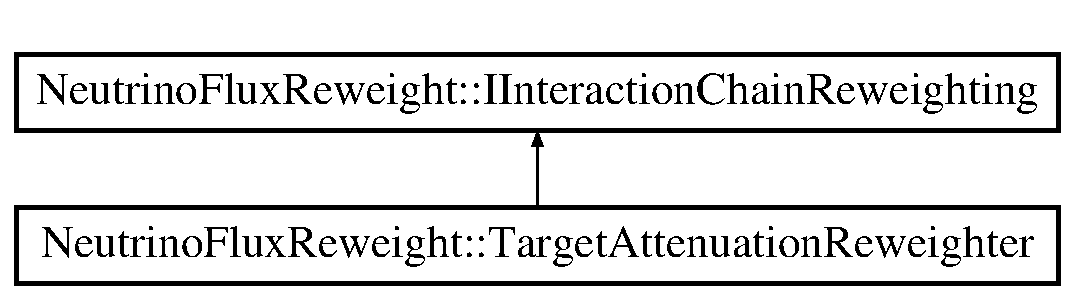
\includegraphics[height=2.000000cm]{class_neutrino_flux_reweight_1_1_target_attenuation_reweighter}
\end{center}
\end{figure}
\subsection*{Public Member Functions}
\begin{DoxyCompactItemize}
\item 
\hyperlink{class_neutrino_flux_reweight_1_1_target_attenuation_reweighter_a4bdac10057844c185c68a6126c85b29a}{Target\-Attenuation\-Reweighter} (int iuniv, const \hyperlink{class_neutrino_flux_reweight_1_1_parameter_table}{Parameter\-Table} \&cv\-\_\-pars, const \hyperlink{class_neutrino_flux_reweight_1_1_parameter_table}{Parameter\-Table} \&univ\-\_\-pars)
\item 
virtual \hyperlink{class_neutrino_flux_reweight_1_1_target_attenuation_reweighter_a00969fcc70150ea19dce58799742c8ca}{$\sim$\-Target\-Attenuation\-Reweighter} ()
\item 
virtual std\-::vector$<$ bool $>$ \hyperlink{class_neutrino_flux_reweight_1_1_target_attenuation_reweighter_a99789f168f16b45ebf5b02dad6f86cb5}{can\-Reweight} (const \hyperlink{class_neutrino_flux_reweight_1_1_interaction_chain_data}{Interaction\-Chain\-Data} \&aa)
\begin{DoxyCompactList}\small\item\em Look through the \hyperlink{class_neutrino_flux_reweight_1_1_interaction_chain_data}{Interaction\-Chain\-Data} input and identify those Interactions that can be reweighted as part of a chain. We return a vector indicating which elements will be assigned a weight by calculate\-Weight. \end{DoxyCompactList}\item 
virtual double \hyperlink{class_neutrino_flux_reweight_1_1_target_attenuation_reweighter_a58691aeda33f770a28cd27f677ae790f}{calculate\-Weight} (const \hyperlink{class_neutrino_flux_reweight_1_1_interaction_chain_data}{Interaction\-Chain\-Data} \&aa)
\begin{DoxyCompactList}\small\item\em calculate a weight for this interaction chain given the central value parameters and the parameters for this universe. The weight is something like\-: f(cv)/f(M\-C) $\ast$ f(univ)/f(cv) where cv in this case corresponds to the best value of the parameter, given the data. If univ\-\_\-pars=cv\-\_\-pars then we are calculating a central value weight. Note, \hyperlink{class_neutrino_flux_reweight_1_1_target_attenuation_reweighter_a99789f168f16b45ebf5b02dad6f86cb5}{can\-Reweight()} should be called to determine which elements of the chain are covered by the weight returned by \hyperlink{class_neutrino_flux_reweight_1_1_target_attenuation_reweighter_a58691aeda33f770a28cd27f677ae790f}{calculate\-Weight()} \end{DoxyCompactList}\end{DoxyCompactItemize}
\subsection*{Static Public Member Functions}
\begin{DoxyCompactItemize}
\item 
static double \hyperlink{class_neutrino_flux_reweight_1_1_target_attenuation_reweighter_abc3651ca760b302a9eb1590e2a2abcc7}{target\-Start\-Z} (const std\-::string \&tgtcfg)
\item 
static double \hyperlink{class_neutrino_flux_reweight_1_1_target_attenuation_reweighter_abffb4bb0215666bf54f96a561f6fbcde}{shift\-Playlist} (const int ipl)
\begin{DoxyCompactList}\small\item\em Get the additional shift for the Minerva playlist if this is defined. \end{DoxyCompactList}\item 
static bool \hyperlink{class_neutrino_flux_reweight_1_1_target_attenuation_reweighter_a92d081ff9e771a79919287fba68b7a94}{is\-M\-E} (const std\-::string \&tgtcfg)
\begin{DoxyCompactList}\small\item\em does the configuration correspond to the M\-E beam? \end{DoxyCompactList}\item 
static bool \hyperlink{class_neutrino_flux_reweight_1_1_target_attenuation_reweighter_a675884a2ca166868e55bb1d6c2eac321}{is\-L\-E} (const std\-::string \&tgtcfg)
\begin{DoxyCompactList}\small\item\em does the configuration correspond to the L\-E beam? \end{DoxyCompactList}\item 
static double \hyperlink{class_neutrino_flux_reweight_1_1_target_attenuation_reweighter_a456b05db5e17fef740619e47c18eabcf}{get\-Target\-Penetration\-L\-E} (double z\-\_\-start, double z\-\_\-end, double z0\-\_\-budal)
\item 
static double \hyperlink{class_neutrino_flux_reweight_1_1_target_attenuation_reweighter_a69653c6ab68bdf8836d80a302cb818c1}{get\-Target\-Penetration\-M\-E} (double z\-\_\-start, double z\-\_\-end, double z0\-\_\-budal)
\item 
static double \hyperlink{class_neutrino_flux_reweight_1_1_target_attenuation_reweighter_a1e7273b417c1013b777ab3532da5ef5e}{get\-Z\-Tgt\-Exit} (double pos\-\_\-start\mbox{[}$\,$\mbox{]}, double mom\-\_\-start\mbox{[}$\,$\mbox{]}, bool leflag, bool meflag)
\end{DoxyCompactItemize}
\subsection*{Private Attributes}
\begin{DoxyCompactItemize}
\item 
const \hyperlink{class_neutrino_flux_reweight_1_1_parameter_table}{Parameter\-Table} \& \hyperlink{class_neutrino_flux_reweight_1_1_target_attenuation_reweighter_a57e907b9b35335e57c20b7280e016725}{cv\-Pars}
\item 
const \hyperlink{class_neutrino_flux_reweight_1_1_parameter_table}{Parameter\-Table} \& \hyperlink{class_neutrino_flux_reweight_1_1_target_attenuation_reweighter_a7c23916d46501cf3e0ff3211830d9412}{univ\-Pars}
\item 
int \hyperlink{class_neutrino_flux_reweight_1_1_target_attenuation_reweighter_ad8c3e794f3e8dec8e728f19accea6dd2}{i\-Univ}
\item 
float \hyperlink{class_neutrino_flux_reweight_1_1_target_attenuation_reweighter_aeffa7cad0d6106661a216901a5304ff8}{prod\-\_\-prt\-C\-\_\-xsec}
\item 
float \hyperlink{class_neutrino_flux_reweight_1_1_target_attenuation_reweighter_a69d6f0a9aae695e7abb4484bf3dce015}{qe\-\_\-prt\-C\-\_\-xsec}
\item 
float \hyperlink{class_neutrino_flux_reweight_1_1_target_attenuation_reweighter_afe869ddec31e4710192f0a990b78c7b6}{delta\-\_\-sigma\-\_\-pi\-C\-\_\-xsec}
\item 
float \hyperlink{class_neutrino_flux_reweight_1_1_target_attenuation_reweighter_abcfaf35e7861c941eb17a22a9fdc867d}{delta\-\_\-sigma\-\_\-kap\-C\-\_\-xsec\-\_\-low\-P}
\item 
float \hyperlink{class_neutrino_flux_reweight_1_1_target_attenuation_reweighter_a1da8f3585af2ed5e282e6f2cd7e613f9}{delta\-\_\-sigma\-\_\-kap\-C\-\_\-xsec\-\_\-high\-P}
\item 
float \hyperlink{class_neutrino_flux_reweight_1_1_target_attenuation_reweighter_a83c1ebd3f9ce871a6aeefb52f9fd1dbc}{delta\-\_\-sigma\-\_\-kam\-C\-\_\-xsec\-\_\-low\-P}
\item 
float \hyperlink{class_neutrino_flux_reweight_1_1_target_attenuation_reweighter_a95594f470ba874e6497c656e73de5af0}{delta\-\_\-sigma\-\_\-kam\-C\-\_\-xsec\-\_\-high\-P}
\end{DoxyCompactItemize}


\subsection{Detailed Description}
Reweight to account for attenuation of the beam in the target. 

If the M\-C does not get the reaction cross-\/section correct the number of interactions in the target, the number of primary protons which do not interact in the target, and the distribution of interactions along z are affected. M\-I\-P\-P measures yields per incoming proton, not per interaction, so their measurment includes the probability of interaction and also the yield per interaction. 

Definition at line 21 of file Target\-Attenuation\-Reweighter.\-h.



\subsection{Constructor \& Destructor Documentation}
\hypertarget{class_neutrino_flux_reweight_1_1_target_attenuation_reweighter_a4bdac10057844c185c68a6126c85b29a}{\index{Neutrino\-Flux\-Reweight\-::\-Target\-Attenuation\-Reweighter@{Neutrino\-Flux\-Reweight\-::\-Target\-Attenuation\-Reweighter}!Target\-Attenuation\-Reweighter@{Target\-Attenuation\-Reweighter}}
\index{Target\-Attenuation\-Reweighter@{Target\-Attenuation\-Reweighter}!NeutrinoFluxReweight::TargetAttenuationReweighter@{Neutrino\-Flux\-Reweight\-::\-Target\-Attenuation\-Reweighter}}
\subsubsection[{Target\-Attenuation\-Reweighter}]{\setlength{\rightskip}{0pt plus 5cm}Neutrino\-Flux\-Reweight\-::\-Target\-Attenuation\-Reweighter\-::\-Target\-Attenuation\-Reweighter (
\begin{DoxyParamCaption}
\item[{int}]{iuniv, }
\item[{const {\bf Parameter\-Table} \&}]{cv\-\_\-pars, }
\item[{const {\bf Parameter\-Table} \&}]{univ\-\_\-pars}
\end{DoxyParamCaption}
)}}\label{class_neutrino_flux_reweight_1_1_target_attenuation_reweighter_a4bdac10057844c185c68a6126c85b29a}


Definition at line 21 of file Target\-Attenuation\-Reweighter.\-cpp.


\begin{DoxyCode}
22     :\hyperlink{class_neutrino_flux_reweight_1_1_target_attenuation_reweighter_a57e907b9b35335e57c20b7280e016725}{cvPars}(cv\_pars),\hyperlink{class_neutrino_flux_reweight_1_1_target_attenuation_reweighter_a7c23916d46501cf3e0ff3211830d9412}{univPars}(univ\_pars),\hyperlink{class_neutrino_flux_reweight_1_1_target_attenuation_reweighter_ad8c3e794f3e8dec8e728f19accea6dd2}{iUniv}(iuniv)\{
23     
24     \textcolor{comment}{// const boost::interprocess::flat\_map<std::string, double>& this\_table = univPars.getMap();}
25      \hyperlink{class_neutrino_flux_reweight_1_1_target_attenuation_reweighter_aeffa7cad0d6106661a216901a5304ff8}{prod\_prtC\_xsec} = \hyperlink{class_neutrino_flux_reweight_1_1_target_attenuation_reweighter_a7c23916d46501cf3e0ff3211830d9412}{univPars}.\hyperlink{class_neutrino_flux_reweight_1_1_parameter_table_acb7dc8335b65b116f6092f2fa57ca5ed}{getParameterValue}(\textcolor{stringliteral}{"prod\_prtC\_xsec"});
26      \hyperlink{class_neutrino_flux_reweight_1_1_target_attenuation_reweighter_a69d6f0a9aae695e7abb4484bf3dce015}{qe\_prtC\_xsec}   = \hyperlink{class_neutrino_flux_reweight_1_1_target_attenuation_reweighter_a7c23916d46501cf3e0ff3211830d9412}{univPars}.\hyperlink{class_neutrino_flux_reweight_1_1_parameter_table_acb7dc8335b65b116f6092f2fa57ca5ed}{getParameterValue}(\textcolor{stringliteral}{"qe\_prtC\_xsec"});
27      \hyperlink{class_neutrino_flux_reweight_1_1_target_attenuation_reweighter_afe869ddec31e4710192f0a990b78c7b6}{delta\_sigma\_piC\_xsec} = \hyperlink{class_neutrino_flux_reweight_1_1_target_attenuation_reweighter_a7c23916d46501cf3e0ff3211830d9412}{univPars}.
      \hyperlink{class_neutrino_flux_reweight_1_1_parameter_table_acb7dc8335b65b116f6092f2fa57ca5ed}{getParameterValue}(\textcolor{stringliteral}{"inel\_piC\_xsec"});
28      \hyperlink{class_neutrino_flux_reweight_1_1_target_attenuation_reweighter_abcfaf35e7861c941eb17a22a9fdc867d}{delta\_sigma\_kapC\_xsec\_lowP}  = \hyperlink{class_neutrino_flux_reweight_1_1_target_attenuation_reweighter_a7c23916d46501cf3e0ff3211830d9412}{univPars}.
      \hyperlink{class_neutrino_flux_reweight_1_1_parameter_table_acb7dc8335b65b116f6092f2fa57ca5ed}{getParameterValue}(\textcolor{stringliteral}{"inel\_kapC\_xsec\_lowP"});
29      \hyperlink{class_neutrino_flux_reweight_1_1_target_attenuation_reweighter_a1da8f3585af2ed5e282e6f2cd7e613f9}{delta\_sigma\_kapC\_xsec\_highP} = \hyperlink{class_neutrino_flux_reweight_1_1_target_attenuation_reweighter_a7c23916d46501cf3e0ff3211830d9412}{univPars}.
      \hyperlink{class_neutrino_flux_reweight_1_1_parameter_table_acb7dc8335b65b116f6092f2fa57ca5ed}{getParameterValue}(\textcolor{stringliteral}{"inel\_kapC\_xsec\_highP"});
30      \hyperlink{class_neutrino_flux_reweight_1_1_target_attenuation_reweighter_a83c1ebd3f9ce871a6aeefb52f9fd1dbc}{delta\_sigma\_kamC\_xsec\_lowP}  = \hyperlink{class_neutrino_flux_reweight_1_1_target_attenuation_reweighter_a7c23916d46501cf3e0ff3211830d9412}{univPars}.
      \hyperlink{class_neutrino_flux_reweight_1_1_parameter_table_acb7dc8335b65b116f6092f2fa57ca5ed}{getParameterValue}(\textcolor{stringliteral}{"inel\_kamC\_xsec\_lowP"});
31      \hyperlink{class_neutrino_flux_reweight_1_1_target_attenuation_reweighter_a95594f470ba874e6497c656e73de5af0}{delta\_sigma\_kamC\_xsec\_highP} = \hyperlink{class_neutrino_flux_reweight_1_1_target_attenuation_reweighter_a7c23916d46501cf3e0ff3211830d9412}{univPars}.
      \hyperlink{class_neutrino_flux_reweight_1_1_parameter_table_acb7dc8335b65b116f6092f2fa57ca5ed}{getParameterValue}(\textcolor{stringliteral}{"inel\_kamC\_xsec\_highP"});
32 
33   \}
\end{DoxyCode}
\hypertarget{class_neutrino_flux_reweight_1_1_target_attenuation_reweighter_a00969fcc70150ea19dce58799742c8ca}{\index{Neutrino\-Flux\-Reweight\-::\-Target\-Attenuation\-Reweighter@{Neutrino\-Flux\-Reweight\-::\-Target\-Attenuation\-Reweighter}!$\sim$\-Target\-Attenuation\-Reweighter@{$\sim$\-Target\-Attenuation\-Reweighter}}
\index{$\sim$\-Target\-Attenuation\-Reweighter@{$\sim$\-Target\-Attenuation\-Reweighter}!NeutrinoFluxReweight::TargetAttenuationReweighter@{Neutrino\-Flux\-Reweight\-::\-Target\-Attenuation\-Reweighter}}
\subsubsection[{$\sim$\-Target\-Attenuation\-Reweighter}]{\setlength{\rightskip}{0pt plus 5cm}Neutrino\-Flux\-Reweight\-::\-Target\-Attenuation\-Reweighter\-::$\sim$\-Target\-Attenuation\-Reweighter (
\begin{DoxyParamCaption}
{}
\end{DoxyParamCaption}
)\hspace{0.3cm}{\ttfamily [virtual]}}}\label{class_neutrino_flux_reweight_1_1_target_attenuation_reweighter_a00969fcc70150ea19dce58799742c8ca}


Definition at line 34 of file Target\-Attenuation\-Reweighter.\-cpp.


\begin{DoxyCode}
34                                                            \{
35     
36   \}
\end{DoxyCode}


\subsection{Member Function Documentation}
\hypertarget{class_neutrino_flux_reweight_1_1_target_attenuation_reweighter_a58691aeda33f770a28cd27f677ae790f}{\index{Neutrino\-Flux\-Reweight\-::\-Target\-Attenuation\-Reweighter@{Neutrino\-Flux\-Reweight\-::\-Target\-Attenuation\-Reweighter}!calculate\-Weight@{calculate\-Weight}}
\index{calculate\-Weight@{calculate\-Weight}!NeutrinoFluxReweight::TargetAttenuationReweighter@{Neutrino\-Flux\-Reweight\-::\-Target\-Attenuation\-Reweighter}}
\subsubsection[{calculate\-Weight}]{\setlength{\rightskip}{0pt plus 5cm}double Neutrino\-Flux\-Reweight\-::\-Target\-Attenuation\-Reweighter\-::calculate\-Weight (
\begin{DoxyParamCaption}
\item[{const {\bf Interaction\-Chain\-Data} \&}]{}
\end{DoxyParamCaption}
)\hspace{0.3cm}{\ttfamily [virtual]}}}\label{class_neutrino_flux_reweight_1_1_target_attenuation_reweighter_a58691aeda33f770a28cd27f677ae790f}


calculate a weight for this interaction chain given the central value parameters and the parameters for this universe. The weight is something like\-: f(cv)/f(M\-C) $\ast$ f(univ)/f(cv) where cv in this case corresponds to the best value of the parameter, given the data. If univ\-\_\-pars=cv\-\_\-pars then we are calculating a central value weight. Note, \hyperlink{class_neutrino_flux_reweight_1_1_target_attenuation_reweighter_a99789f168f16b45ebf5b02dad6f86cb5}{can\-Reweight()} should be called to determine which elements of the chain are covered by the weight returned by \hyperlink{class_neutrino_flux_reweight_1_1_target_attenuation_reweighter_a58691aeda33f770a28cd27f677ae790f}{calculate\-Weight()} 



Implements \hyperlink{class_neutrino_flux_reweight_1_1_i_interaction_chain_reweighting_ae28403553637013fdc720674ee24c7c5}{Neutrino\-Flux\-Reweight\-::\-I\-Interaction\-Chain\-Reweighting}.



Definition at line 81 of file Target\-Attenuation\-Reweighter.\-cpp.


\begin{DoxyCode}
81                                                                                    \{
82     std::string mode(getenv(\textcolor{stringliteral}{"MODE"}));
83     \textcolor{keywordtype}{double} wgt =1.0;
84     
85     MakeReweight*  makerew =  \hyperlink{class_neutrino_flux_reweight_1_1_make_reweight_a42d1fa92a1e30bd80538188e0c9d8b4a}{MakeReweight::getInstance}();
86     \textcolor{keywordtype}{bool} domipp = (makerew->cv\_rw)->doMIPPNumi;
87 
88     \textcolor{comment}{//Some constants:}
89     \textcolor{keyword}{const} \textcolor{keywordtype}{double} graphite\_density=1.78;\textcolor{comment}{// g/cc}
90     \textcolor{keyword}{const} \textcolor{keywordtype}{double} avog\_x\_mb2cm2 = 6.02214e-4; \textcolor{comment}{//useful constant}
91     \textcolor{keyword}{const} \textcolor{keywordtype}{double} graphite\_A    = 12.01; \textcolor{comment}{// g/mole    }
92 
93     std::vector<InteractionData> vec\_inter = aa.interaction\_chain;
94 
95     \textcolor{comment}{//Finding the Data and MC total cross sections:    }
96     AttenuationMC* dtH = \hyperlink{class_neutrino_flux_reweight_1_1_attenuation_m_c_acc338217e771bf334014ed943015e6a1}{AttenuationMC::getInstance}();
97     MIPPNumiYieldsBins*  MIPPbins =  \hyperlink{class_neutrino_flux_reweight_1_1_m_i_p_p_numi_yields_bins_a7f44afe90a846812d6eabfafa8f576e4}{MIPPNumiYieldsBins::getInstance}();
98    
99     \textcolor{keywordtype}{bool} there\_is\_MIPP  = \textcolor{keyword}{false};
100     \textcolor{keywordtype}{bool} it\_is\_survival = \textcolor{keyword}{false};
101     
102     \textcolor{comment}{//MIPP:}
103     TargetData tar = aa.tar\_info;
104     \textcolor{keywordtype}{int} binID = MIPPbins->BinID(tar.Pz,tar.Pt,tar.Tar\_pdg);   
105     \textcolor{keywordtype}{bool} is\_le = \hyperlink{class_neutrino_flux_reweight_1_1_target_attenuation_reweighter_a675884a2ca166868e55bb1d6c2eac321}{isLE}(aa.target\_config);
106     \textcolor{keywordtype}{bool} is\_me = \hyperlink{class_neutrino_flux_reweight_1_1_target_attenuation_reweighter_a92d081ff9e771a79919287fba68b7a94}{isME}(aa.target\_config);
107     \textcolor{keywordflow}{if}( !is\_le &&  !is\_me )\{
108       \textcolor{keywordflow}{throw} std::runtime\_error(\textcolor{stringliteral}{"cannot determine if it's LE or ME beam"});
109     \}
110 
111     TH1D* hzpos;
112     \textcolor{keywordflow}{if}(binID>=0)\{
113        \textcolor{keywordflow}{if}(tar.Tar\_pdg == 211 || tar.Tar\_pdg ==- 211)\{
114         there\_is\_MIPP = \textcolor{keyword}{true};
115         \textcolor{keywordflow}{if}(tar.Tar\_pdg == 211 && is\_le)hzpos = dtH->hzpostgt\_pip\_le[binID];
116         \textcolor{keywordflow}{if}(tar.Tar\_pdg == 211 && is\_me)hzpos = dtH->hzpostgt\_pip\_me[binID];
117         \textcolor{keywordflow}{if}(tar.Tar\_pdg ==-211 && is\_le)hzpos = dtH->hzpostgt\_pim\_le[binID];
118         \textcolor{keywordflow}{if}(tar.Tar\_pdg ==-211 && is\_me)hzpos = dtH->hzpostgt\_pim\_me[binID];
119        \}
120        \textcolor{keywordflow}{else} \textcolor{keywordflow}{if}(tar.Tar\_pdg == 321)\{
121          \textcolor{keywordtype}{int} aux\_binID = MIPPbins->BinID(tar.Pz,tar.Pt,211);
122          \textcolor{keywordflow}{if}(aux\_binID>=0)\{
123            there\_is\_MIPP = \textcolor{keyword}{true};
124            \textcolor{comment}{//I substracted 78 because we store all histos in AttenuationMC but the kaon histograms make }
125            \textcolor{comment}{// sense after P>20 GeV/c and we are using bin ID convention here.}
126            \textcolor{keywordflow}{if}(is\_le)hzpos = dtH->hzpostgt\_kap\_le[aux\_binID-78];
127            \textcolor{keywordflow}{if}(is\_me)hzpos = dtH->hzpostgt\_kap\_me[aux\_binID-78];
128          \}
129        \}
130        \textcolor{keywordflow}{else} \textcolor{keywordflow}{if}(tar.Tar\_pdg == -321)\{
131          \textcolor{keywordtype}{int} aux\_binID = MIPPbins->BinID(tar.Pz,tar.Pt,-211);
132          \textcolor{keywordflow}{if}(aux\_binID>=0)\{
133            there\_is\_MIPP = \textcolor{keyword}{true};
134            \textcolor{keywordflow}{if}(is\_le)hzpos = dtH->hzpostgt\_kam\_le[aux\_binID-78];
135            \textcolor{keywordflow}{if}(is\_me)hzpos = dtH->hzpostgt\_kam\_me[aux\_binID-78];
136          \}
137        \}
138        \textcolor{keywordflow}{else} \textcolor{keywordflow}{if}(tar.Tar\_pdg == 130 || tar.Tar\_pdg == 310)\{
139          \textcolor{keywordtype}{int} aux\_binID = MIPPbins->BinID(tar.Pz,tar.Pt,211);
140          \textcolor{keywordflow}{if}(aux\_binID>=0)\{
141            there\_is\_MIPP = \textcolor{keyword}{true};
142            \textcolor{keywordflow}{if}(is\_le)hzpos = dtH->hzpostgt\_kap\_le[aux\_binID-78];
143            \textcolor{keywordflow}{if}(is\_me)hzpos = dtH->hzpostgt\_kap\_me[aux\_binID-78];
144          \}
145        \}
146        \textcolor{keywordflow}{else}\{
147          std::cout<<\textcolor{stringliteral}{"=> There is an in MIPPNumiYieldsBins"}<<std::endl;
148        \}
149     \}
150     
151     \textcolor{comment}{//Survival:}
152     \textcolor{keywordflow}{if}(!there\_is\_MIPP && vec\_inter[0].Vol!=\textcolor{stringliteral}{"BudalMonitor"} && vec\_inter[0].Vol!=\textcolor{stringliteral}{"TGT1"} && vec\_inter[0].Vol!=\textcolor{stringliteral}{
      "Budal\_HFVS"} && vec\_inter[0].Vol!=\textcolor{stringliteral}{"Budal\_VFHS"})\{
153       it\_is\_survival = \textcolor{keyword}{true};
154     \}    
155     \textcolor{keywordflow}{if}((mode==\textcolor{stringliteral}{"REF"})||(mode==\textcolor{stringliteral}{"OPT"}))\{
156       \textcolor{keywordflow}{if}(!there\_is\_MIPP && vec\_inter[0].Vol!=\textcolor{stringliteral}{"TargetFinHorizontal"} && vec\_inter[0].Vol!=\textcolor{stringliteral}{"
      TargetNoSplitSegment"} && vec\_inter[0].Vol!=\textcolor{stringliteral}{"tCoreLog"})\{
157 
158         it\_is\_survival = \textcolor{keyword}{true};
159       \}
160     \}
161     
162     \textcolor{keywordtype}{double} delta\_sigma = 0.0; \textcolor{comment}{// sigma\_data - sigma\_mc}
163     \textcolor{keywordtype}{double} ratio\_sigma = 0.0; \textcolor{comment}{// sigma\_data / sigma\_mc}
164 
165     delta\_sigma  = \hyperlink{class_neutrino_flux_reweight_1_1_target_attenuation_reweighter_aeffa7cad0d6106661a216901a5304ff8}{prod\_prtC\_xsec};
166     delta\_sigma  += \hyperlink{class_neutrino_flux_reweight_1_1_target_attenuation_reweighter_a69d6f0a9aae695e7abb4484bf3dce015}{qe\_prtC\_xsec}; 
167     
168     \textcolor{keywordtype}{int} binpartC = (dtH->hXS\_prtC)->FindBin(vec\_inter[0].Inc\_P);
169     \textcolor{keywordtype}{double} mcval = (dtH->hXS\_prtC)->GetBinContent(binpartC);
170     \textcolor{keywordflow}{if}(mcval<1.e-12)\{
171       std::cout<<\textcolor{stringliteral}{"This seems especial cases in which the proton interact before the target (Air?). we need
       to investigate it."}<<\textcolor{stringliteral}{" Inc\_P "}<<vec\_inter[0].Inc\_P<<std::endl;
172       \textcolor{keywordflow}{return} 1.;
173     \}
174     ratio\_sigma = delta\_sigma / mcval;
175     delta\_sigma -= mcval;
176     
177     \textcolor{comment}{//Finding the target penetration for the primary proton beam:}
178    
179     \textcolor{keywordtype}{double} startZ        = \hyperlink{class_neutrino_flux_reweight_1_1_target_attenuation_reweighter_abc3651ca760b302a9eb1590e2a2abcc7}{targetStartZ}(aa.target\_config) + 
      \hyperlink{class_neutrino_flux_reweight_1_1_target_attenuation_reweighter_abffb4bb0215666bf54f96a561f6fbcde}{shiftPlaylist}(aa.playlist);
180     \textcolor{keywordtype}{double} endZ = (vec\_inter[0].Vtx)[2];
181     \textcolor{keywordtype}{double} totmatZ = 0.;  \textcolor{comment}{//this will be the amount of material passed. }
182 
183     \textcolor{keywordflow}{if}( is\_le)\{
184       \textcolor{comment}{//check of initial z position:}
185       \textcolor{keywordflow}{if}(vec\_inter[0].Vol==\textcolor{stringliteral}{"BudalMonitor"})\{
186         \textcolor{keywordflow}{if}(endZ<startZ || endZ>(startZ+2.0))std::cout<<\textcolor{stringliteral}{"Potential error of BudalMonitor=> startZ, endZ: "}<<
      startZ<<\textcolor{stringliteral}{" "}<<endZ<<std::endl;   
187       \}      
188       \textcolor{keywordflow}{if}((mode==\textcolor{stringliteral}{"OPT"})||(mode==\textcolor{stringliteral}{"REF"}))\{
189         \textcolor{keywordflow}{if}(vec\_inter[0].Vol==\textcolor{stringliteral}{"TargetFinHorizontal"})\{
190           \textcolor{keywordflow}{if}(endZ<startZ || endZ>(startZ+2.0))std::cout<<\textcolor{stringliteral}{"Potential error of BudalMonitor=> startZ, endZ: "}
      <<startZ<<\textcolor{stringliteral}{" "}<<endZ<<std::endl;   
191         \}
192       \}
193       totmatZ = \hyperlink{class_neutrino_flux_reweight_1_1_target_attenuation_reweighter_a456b05db5e17fef740619e47c18eabcf}{getTargetPenetrationLE}(startZ,endZ,startZ);
194      \textcolor{comment}{// std::cout<<"TargetAttenuation:: Start Z "<<startZ<<" End Z "<<endZ<<" totMatZ "<<totmatZ<<"
       "<<vec\_inter[0].Vol<<std::endl;}
195     \}
196     \textcolor{keywordflow}{else} \textcolor{keywordflow}{if}( is\_me )\{ 
197       \textcolor{comment}{//check of initial z position:}
198       \textcolor{keywordflow}{if}(vec\_inter[0].Vol==\textcolor{stringliteral}{"Budal\_HFVS"})\{
199         \textcolor{keywordflow}{if}(endZ<startZ || endZ>(startZ+2.4))std::cout<<\textcolor{stringliteral}{"Potential error of Budal\_HFVS => startZ, endZ: "}<<
      startZ<<\textcolor{stringliteral}{" "}<<endZ<<std::endl;   
200       \}
201       totmatZ = \hyperlink{class_neutrino_flux_reweight_1_1_target_attenuation_reweighter_a69653c6ab68bdf8836d80a302cb818c1}{getTargetPenetrationME}(startZ,endZ,startZ);
202     \}   
203 
204     \textcolor{keywordflow}{if}(totmatZ<0)totmatZ=0;
205     
206     totmatZ *= avog\_x\_mb2cm2;
207     totmatZ /= graphite\_A;
208     totmatZ *= graphite\_density;
209 
210     \textcolor{comment}{//Calculating the weight:}
211     \textcolor{keywordtype}{double} norm = 1.0;
212     \textcolor{keywordflow}{if}(there\_is\_MIPP && domipp)\{
213       \textcolor{keywordtype}{int} nbins = hzpos->GetXaxis()->GetNbins();
214       \textcolor{keywordtype}{double} integral\_mc = 0;
215       \textcolor{keywordtype}{double} integral\_wt = 0;
216       \textcolor{keywordflow}{for}(\textcolor{keywordtype}{int} ib=1;ib<=nbins;ib++)\{
217         \textcolor{keywordtype}{double} cont = hzpos->GetBinContent(ib);
218         \textcolor{keywordtype}{double} crr  = hzpos->GetXaxis()->GetBinCenter(ib);
219         integral\_mc += cont;    
220         integral\_wt += cont*ratio\_sigma*exp(-1.0*crr*avog\_x\_mb2cm2*graphite\_density*delta\_sigma/graphite\_A)
      ;
221       \}
222       \textcolor{keywordflow}{if}(integral\_wt<=0 || integral\_mc<=0)\{
223         \textcolor{keywordflow}{throw} std::runtime\_error(\textcolor{stringliteral}{"yield is zero or negative... check!"});
224       \}     
225       norm = integral\_mc/integral\_wt;
226     \}
227     
228     \textcolor{comment}{//Calculating the weight for the primary:}
229     \textcolor{keywordtype}{double} wgt\_pri = 1.0;
230     
231     \textcolor{keywordflow}{if}(it\_is\_survival)\{
232       wgt\_pri = exp(-1.0*totmatZ*delta\_sigma);
233     \}
234     \textcolor{keywordflow}{else}\{
235       wgt\_pri = norm*ratio\_sigma*exp(-1.0*totmatZ*delta\_sigma);
236     \}
237     
238     \textcolor{comment}{//Calculating the weight for secondaries, tertiaries, etc:}
239     \textcolor{keywordtype}{double} wgt\_sec = 1.0;
240     \textcolor{keywordflow}{if}(!domipp)\{
241       \textcolor{keywordflow}{for}(\textcolor{keywordtype}{size\_t} ii=1;ii<vec\_inter.size();ii++)\{
242         \textcolor{keywordtype}{bool} starts\_tgt = vec\_inter[ii-1].Vol == \textcolor{stringliteral}{"BudalMonitor"} || vec\_inter[ii-1].Vol == \textcolor{stringliteral}{"TGT1"} || 
      vec\_inter[ii-1].Vol == \textcolor{stringliteral}{"Budal\_HFVS"}  || vec\_inter[ii-1].Vol == \textcolor{stringliteral}{"Budal\_VFHS"};
243         \textcolor{keywordflow}{if}((mode==\textcolor{stringliteral}{"REF"})||(mode==\textcolor{stringliteral}{"OPT"}))\{
244           starts\_tgt = vec\_inter[ii-1].Vol == \textcolor{stringliteral}{"TargetFinHorizontal"} || vec\_inter[ii-1].Vol == \textcolor{stringliteral}{"
      TargetNoSplitSegment"}|| vec\_inter[ii-1].Vol == \textcolor{stringliteral}{"tCoreLog"};
245         \}
246         \textcolor{keywordflow}{if}(!starts\_tgt)\textcolor{keywordflow}{continue};
247         \textcolor{keywordtype}{bool} ends\_tgt = vec\_inter[ii].Vol   == \textcolor{stringliteral}{"BudalMonitor"} || vec\_inter[ii].Vol   == \textcolor{stringliteral}{"TGT1"} || vec\_inter
      [ii].Vol   == \textcolor{stringliteral}{"Budal\_HFVS"}  || vec\_inter[ii].Vol   == \textcolor{stringliteral}{"Budal\_VFHS"};
248         \textcolor{keywordflow}{if}((mode==\textcolor{stringliteral}{"REF"})||(mode==\textcolor{stringliteral}{"OPT"}))\{
249           ends\_tgt = vec\_inter[ii].Vol   == \textcolor{stringliteral}{"TargetFinHorizontal"} || vec\_inter[ii].Vol   == \textcolor{stringliteral}{"
      TargetNoSplitSegment"} || vec\_inter[ii].Vol == \textcolor{stringliteral}{"tCoreLog"};
250         \}
251         \textcolor{comment}{//double totmatR  = 0.0;}
252         \textcolor{keywordtype}{double} dsigma   = 0.0;
253         \textcolor{keywordtype}{double} fact\_int = 1.0;  
254         \textcolor{keywordtype}{double} fact     = 1.0;  
255         \textcolor{comment}{//dsigma and fact\_int:}
256         \textcolor{keywordflow}{if}(vec\_inter[ii].Inc\_pdg==2212)\{
257           dsigma   = delta\_sigma;
258           binpartC = (dtH->hXS\_prtC)->FindBin(vec\_inter[ii].Inc\_P);
259           mcval    = (dtH->hXS\_prtC)->GetBinContent(binpartC);
260           fact\_int = (dsigma+mcval)/mcval;
261         \}
262         \textcolor{keywordflow}{else} \textcolor{keywordflow}{if}(vec\_inter[ii].Inc\_pdg==211 || vec\_inter[ii].Inc\_pdg==-211)\{
263           dsigma   = \hyperlink{class_neutrino_flux_reweight_1_1_target_attenuation_reweighter_afe869ddec31e4710192f0a990b78c7b6}{delta\_sigma\_piC\_xsec};
264           binpartC = (dtH->hXS\_piC)->FindBin(vec\_inter[ii].Inc\_P);
265           mcval    = (dtH->hXS\_piC)->GetBinContent(binpartC);
266           fact\_int = (dsigma+mcval)/mcval;
267         \}
268         \textcolor{keywordflow}{else} \textcolor{keywordflow}{if}(vec\_inter[ii].Inc\_pdg == 321)\{
269           \textcolor{keywordflow}{if}(vec\_inter[ii].Inc\_P<2.0) dsigma = \hyperlink{class_neutrino_flux_reweight_1_1_target_attenuation_reweighter_abcfaf35e7861c941eb17a22a9fdc867d}{delta\_sigma\_kapC\_xsec\_lowP};
270           \textcolor{keywordflow}{if}(vec\_inter[ii].Inc\_P>=2.0)dsigma = \hyperlink{class_neutrino_flux_reweight_1_1_target_attenuation_reweighter_a1da8f3585af2ed5e282e6f2cd7e613f9}{delta\_sigma\_kapC\_xsec\_highP};
271           binpartC = (dtH->hXS\_kapC)->FindBin(vec\_inter[ii].Inc\_P);
272           mcval    = (dtH->hXS\_kapC)->GetBinContent(binpartC);
273           fact\_int = (dsigma+mcval)/mcval;
274         \}
275         \textcolor{keywordflow}{else} \textcolor{keywordflow}{if}(vec\_inter[ii].Inc\_pdg ==-321)\{
276           \textcolor{keywordflow}{if}(vec\_inter[ii].Inc\_P<2.0) dsigma = \hyperlink{class_neutrino_flux_reweight_1_1_target_attenuation_reweighter_a83c1ebd3f9ce871a6aeefb52f9fd1dbc}{delta\_sigma\_kamC\_xsec\_lowP};
277           \textcolor{keywordflow}{if}(vec\_inter[ii].Inc\_P>=2.0)dsigma = \hyperlink{class_neutrino_flux_reweight_1_1_target_attenuation_reweighter_a95594f470ba874e6497c656e73de5af0}{delta\_sigma\_kamC\_xsec\_highP};
278           binpartC = (dtH->hXS\_kamC)->FindBin(vec\_inter[ii].Inc\_P);
279           mcval    = (dtH->hXS\_kamC)->GetBinContent(binpartC);
280           fact\_int = (dsigma+mcval)/mcval;
281         \}
282         \textcolor{keywordflow}{else} \textcolor{keywordflow}{if}(totmatZ<1.e-12)\{
283           dsigma = 0.0;
284           fact\_int = 1.0;
285         \}
286         \textcolor{keywordflow}{else}\{
287           \textcolor{keywordflow}{if}(vec\_inter[ii].Inc\_P<2.0) dsigma = \hyperlink{class_neutrino_flux_reweight_1_1_target_attenuation_reweighter_abcfaf35e7861c941eb17a22a9fdc867d}{delta\_sigma\_kapC\_xsec\_lowP};
288           \textcolor{keywordflow}{if}(vec\_inter[ii].Inc\_P>=2.0)dsigma = \hyperlink{class_neutrino_flux_reweight_1_1_target_attenuation_reweighter_a1da8f3585af2ed5e282e6f2cd7e613f9}{delta\_sigma\_kapC\_xsec\_highP};
289           binpartC = (dtH->hXS\_kapC)->FindBin(vec\_inter[ii].Inc\_P);
290           mcval    = (dtH->hXS\_kapC)->GetBinContent(binpartC);
291           fact\_int = (dsigma+mcval)/mcval;
292         \}
293        \textcolor{keywordflow}{if}(mcval<1.e-12)\{
294        
295       \textcolor{comment}{//std::cout<<"This seems especial cases in which the proton interact before the target (Air?). we
       need to investigate it."<<" Inc\_P "<<vec\_inter[0].Inc\_P<<std::endl;}
296       
297       \textcolor{keywordflow}{return} 1.;
298       
299     \}
300         \textcolor{comment}{//Two cases: 1) ending in th target and leaving the target.}
301         \textcolor{keywordtype}{double} zi = (vec\_inter[ii-1].Vtx)[2];
302         \textcolor{keywordtype}{double} zf = 0.0;
303         \textcolor{keywordflow}{if}(ends\_tgt)\{     
304           zf = (vec\_inter[ii].Vtx)[2];    
305           fact = fact\_int;
306         \}
307         \textcolor{keywordflow}{else} \textcolor{keywordflow}{if}(!ends\_tgt)\{
308           \textcolor{keywordtype}{double} startpart[3] = \{(vec\_inter[ii-1].Vtx)[0],(vec\_inter[ii-1].Vtx)[1],(vec\_inter[ii-1].Vtx)[2]
      \};
309           \textcolor{keywordtype}{double} momtar[3]    = \{tar.Px,tar.Py,tar.Pz\};
310           zf  = \hyperlink{class_neutrino_flux_reweight_1_1_target_attenuation_reweighter_a1e7273b417c1013b777ab3532da5ef5e}{getZTgtExit}(startpart,momtar,is\_le,is\_me);
311         \}
312         \textcolor{keywordflow}{if}(is\_le) totmatZ = \hyperlink{class_neutrino_flux_reweight_1_1_target_attenuation_reweighter_a456b05db5e17fef740619e47c18eabcf}{getTargetPenetrationLE}(zi,zf,startZ);
313         \textcolor{keywordflow}{if}(is\_me) totmatZ = \hyperlink{class_neutrino_flux_reweight_1_1_target_attenuation_reweighter_a69653c6ab68bdf8836d80a302cb818c1}{getTargetPenetrationME}(zi,zf,startZ);
314       
315         \textcolor{keywordflow}{if}(totmatZ<1.e-12)\{
316           dsigma = 0.0;
317           fact = 1.0;
318         \}
319         
320         totmatZ *= avog\_x\_mb2cm2;
321         totmatZ /= graphite\_A;
322         totmatZ *= graphite\_density;    
323         wgt\_sec *= fact*exp(-1.0*totmatZ*dsigma);
324         \textcolor{keywordflow}{if}(isinf(wgt\_sec))std::cout<<\textcolor{stringliteral}{"BAD "}<<zi<<\textcolor{stringliteral}{" "}<<zf<<\textcolor{stringliteral}{" "}<<totmatZ<<\textcolor{stringliteral}{" "}<<startZ<<
325         \textcolor{stringliteral}{" "}<<dsigma<<\textcolor{stringliteral}{" "}<<fact<<std::endl;
326         
327       \}
328     \}
329    \textcolor{comment}{// if(isinf(wgt\_pri*wgt\_sec))std::cout<<wgt\_pri<<" "<<wgt\_sec<<" "<<zi<<" "<<zf<<std::endl;}
330     \textcolor{keywordflow}{return} wgt = wgt\_pri*wgt\_sec;
331     
332   \}
\end{DoxyCode}
\hypertarget{class_neutrino_flux_reweight_1_1_target_attenuation_reweighter_a99789f168f16b45ebf5b02dad6f86cb5}{\index{Neutrino\-Flux\-Reweight\-::\-Target\-Attenuation\-Reweighter@{Neutrino\-Flux\-Reweight\-::\-Target\-Attenuation\-Reweighter}!can\-Reweight@{can\-Reweight}}
\index{can\-Reweight@{can\-Reweight}!NeutrinoFluxReweight::TargetAttenuationReweighter@{Neutrino\-Flux\-Reweight\-::\-Target\-Attenuation\-Reweighter}}
\subsubsection[{can\-Reweight}]{\setlength{\rightskip}{0pt plus 5cm}std\-::vector$<$ bool $>$ Neutrino\-Flux\-Reweight\-::\-Target\-Attenuation\-Reweighter\-::can\-Reweight (
\begin{DoxyParamCaption}
\item[{const {\bf Interaction\-Chain\-Data} \&}]{}
\end{DoxyParamCaption}
)\hspace{0.3cm}{\ttfamily [virtual]}}}\label{class_neutrino_flux_reweight_1_1_target_attenuation_reweighter_a99789f168f16b45ebf5b02dad6f86cb5}


Look through the \hyperlink{class_neutrino_flux_reweight_1_1_interaction_chain_data}{Interaction\-Chain\-Data} input and identify those Interactions that can be reweighted as part of a chain. We return a vector indicating which elements will be assigned a weight by calculate\-Weight. 



Implements \hyperlink{class_neutrino_flux_reweight_1_1_i_interaction_chain_reweighting_aacf17580c1d316f0ebcdfdff7418e9e3}{Neutrino\-Flux\-Reweight\-::\-I\-Interaction\-Chain\-Reweighting}.



Definition at line 37 of file Target\-Attenuation\-Reweighter.\-cpp.


\begin{DoxyCode}
37                                                                                         \{
38     std::vector<bool> can\_rws;
39     std::vector<InteractionData> vec\_inter = aa.interaction\_chain;
40     \textcolor{keywordtype}{int} ninter = vec\_inter.size();
41     std::string mode(getenv(\textcolor{stringliteral}{"MODE"}));
42     \textcolor{comment}{//Looking if there is a proton-Target interaction:}
43     \textcolor{keywordflow}{for}(\textcolor{keywordtype}{int} ii=0;ii<ninter;ii++)\{          
44         \textcolor{keywordflow}{if}(vec\_inter[ii].Inc\_P==0.0)\{
45           can\_rws.push\_back(\textcolor{keyword}{false});
46           \textcolor{keywordflow}{return} can\_rws;
47         \}
48     \textcolor{keywordflow}{if}(ii==0)\{
49       \textcolor{comment}{//first interaction in the target or a primary proton passing through the target }
50 
51         \textcolor{keywordtype}{bool} is\_tgt\_int = vec\_inter[0].Vol == \textcolor{stringliteral}{"BudalMonitor"} || vec\_inter[0].Vol == \textcolor{stringliteral}{"TGT1"} || vec\_inter[0].
      Vol == \textcolor{stringliteral}{"Budal\_HFVS"}  || vec\_inter[0].Vol == \textcolor{stringliteral}{"Budal\_VFHS"};
52         \textcolor{keywordflow}{if}((mode==\textcolor{stringliteral}{"REF"})||(mode==\textcolor{stringliteral}{"OPT"}))\{
53           is\_tgt\_int = vec\_inter[0].Vol == \textcolor{stringliteral}{"TargetFinHorizontal"} || vec\_inter[0].Vol == \textcolor{stringliteral}{"
      TargetNoSplitSegment"} || vec\_inter[0].Vol==\textcolor{stringliteral}{"tCoreLog"};
54         \}
55         \textcolor{keywordflow}{if}(is\_tgt\_int)can\_rws.push\_back(\textcolor{keyword}{true});
56         \textcolor{keywordflow}{else} \textcolor{keywordflow}{if}(vec\_inter[0].Inc\_pdg == 2212)can\_rws.push\_back(\textcolor{keyword}{true});
57         \textcolor{keywordflow}{else} can\_rws.push\_back(\textcolor{keyword}{false});
58       \}
59       \textcolor{comment}{//Absorption in the target of the secondaries:}
60       \textcolor{keywordflow}{else}\{
61         \textcolor{keywordtype}{bool} starts\_tgt = vec\_inter[ii-1].Vol == \textcolor{stringliteral}{"BudalMonitor"} || vec\_inter[ii-1].Vol == \textcolor{stringliteral}{"TGT1"} || 
      vec\_inter[ii-1].Vol == \textcolor{stringliteral}{"Budal\_HFVS"}  || vec\_inter[ii-1].Vol == \textcolor{stringliteral}{"Budal\_VFHS"};
62         \textcolor{keywordtype}{bool} ends\_tgt   = vec\_inter[ii].Vol   == \textcolor{stringliteral}{"BudalMonitor"} || vec\_inter[ii].Vol   == \textcolor{stringliteral}{"TGT1"} || 
      vec\_inter[ii-1].Vol == \textcolor{stringliteral}{"Budal\_HFVS"}  || vec\_inter[ii-1].Vol == \textcolor{stringliteral}{"Budal\_VFHS"};
63         \textcolor{keywordflow}{if}((mode==\textcolor{stringliteral}{"REF"})||(mode==\textcolor{stringliteral}{"OPT"}))\{
64           starts\_tgt = vec\_inter[ii-1].Vol == \textcolor{stringliteral}{"TargetFinHorizontal"} || vec\_inter[ii-1].Vol == \textcolor{stringliteral}{"
      TargetNoSplitSegment"}|| vec\_inter[0].Vol==\textcolor{stringliteral}{"tCoreLog"};
65           ends\_tgt = vec\_inter[ii-1].Vol == \textcolor{stringliteral}{"TargetFinHorizontal"} || vec\_inter[ii-1].Vol == \textcolor{stringliteral}{"
      TargetNoSplitSegment"}||vec\_inter[0].Vol==\textcolor{stringliteral}{"tCoreLog"};
66         \}
67         \textcolor{keywordflow}{if}(starts\_tgt && ends\_tgt)\{
68           can\_rws.push\_back(\textcolor{keyword}{true});
69         \}
70         \textcolor{keywordflow}{else} \textcolor{keywordflow}{if}(starts\_tgt && !ends\_tgt)\{
71           can\_rws.push\_back(\textcolor{keyword}{true});
72         \}
73         \textcolor{keywordflow}{else}\{
74           can\_rws.push\_back(\textcolor{keyword}{false});
75         \}
76       \}
77     \}  
78 
79     \textcolor{keywordflow}{return} can\_rws;
80   \}
\end{DoxyCode}
\hypertarget{class_neutrino_flux_reweight_1_1_target_attenuation_reweighter_a456b05db5e17fef740619e47c18eabcf}{\index{Neutrino\-Flux\-Reweight\-::\-Target\-Attenuation\-Reweighter@{Neutrino\-Flux\-Reweight\-::\-Target\-Attenuation\-Reweighter}!get\-Target\-Penetration\-L\-E@{get\-Target\-Penetration\-L\-E}}
\index{get\-Target\-Penetration\-L\-E@{get\-Target\-Penetration\-L\-E}!NeutrinoFluxReweight::TargetAttenuationReweighter@{Neutrino\-Flux\-Reweight\-::\-Target\-Attenuation\-Reweighter}}
\subsubsection[{get\-Target\-Penetration\-L\-E}]{\setlength{\rightskip}{0pt plus 5cm}double Neutrino\-Flux\-Reweight\-::\-Target\-Attenuation\-Reweighter\-::get\-Target\-Penetration\-L\-E (
\begin{DoxyParamCaption}
\item[{double}]{z\-\_\-start, }
\item[{double}]{z\-\_\-end, }
\item[{double}]{z0\-\_\-budal}
\end{DoxyParamCaption}
)\hspace{0.3cm}{\ttfamily [static]}}}\label{class_neutrino_flux_reweight_1_1_target_attenuation_reweighter_a456b05db5e17fef740619e47c18eabcf}
Returns the amount of target material penetrated by a particle starting at z\-\_\-start and interacting or exiting the target at z\-\_\-end. the upstream edge of the budal monitor must be supplied. All inputs must be in units of cm.

Definition at line 413 of file Target\-Attenuation\-Reweighter.\-cpp.


\begin{DoxyCode}
413                                                                                                          \{\textcolor{comment}{}
414 \textcolor{comment}{    /*!}
415 \textcolor{comment}{     * Returns the amount of target material penetrated by a particle starting at}
416 \textcolor{comment}{     * z\_start and interacting or exiting the target at z\_end.}
417 \textcolor{comment}{     * the upstream edge of the budal monitor must be supplied.}
418 \textcolor{comment}{     * All inputs must be in units of cm.}
419 \textcolor{comment}{     */}
420 
421     \textcolor{comment}{// fin edges determined by printing their position from inside g4numi. }
422     \textcolor{comment}{// coordinate system will need to be translated such that the upstream}
423     \textcolor{comment}{// edge of the budal monitor is at the value returned by target}
424     \textcolor{comment}{// start z.}
425     \textcolor{comment}{// coordinate here in cm}
426     std::string mode(getenv(\textcolor{stringliteral}{"MODE"}));
427     \textcolor{keyword}{const} \textcolor{keywordtype}{int} nfins=48;
428     \textcolor{keyword}{const} \textcolor{keywordtype}{double} us\_edges[nfins]=\{25.4484,   42.1683,   44.1983,   46.2283, 48.2583,
429                                   50.2883,   52.3183,   54.3483,   56.3783,
430                                   58.4083,   60.4383,   62.4683,   64.4983,
431                                   66.5283,   68.5583,   70.5883,   72.6183,
432                                   74.6483,   76.6783,   78.7083,   80.7383,
433                                   82.7683,   84.7983,   86.8283,   88.8583,
434                                   90.8883,   92.9183,   94.9483,   96.9783,
435                                   99.0083,  101.0383,  103.0683,  105.0983,
436                                   107.1283, 109.1583,  111.1883,  113.2183,
437                                   115.2483, 117.2783,  119.3083,  121.3383,
438                                   123.3683, 125.3983,  127.4283,  129.4583,
439                                   131.4883, 133.5183,  135.5483\};
440     \textcolor{keyword}{const} \textcolor{keywordtype}{int} nfins\_ref=49;
441     \textcolor{comment}{//This is for the DUNE reference design target. A. Bashyal                            }
442     \textcolor{keyword}{const} \textcolor{keywordtype}{double} us\_edges\_ref[nfins\_ref]=\{-64.7002,-46.9176,-44.8909, -42.8609, -40.8309, -38.8009, -36.770
      9, 
443                                           -34.7409, -32.7109, -30.6809, -28.6509, -26.6209, -24.5909, 
444                                           -22.5609, -20.5309, -18.5009, -16.4709, -14.4409, -12.4109, -10.3
      809, -8.3509, -6.3209, 
445                                           -4.2909, -2.2609, -0.2309, 1.7991, 3.8291, 5.8591, 7.8891, 9.9191
      , 11.9491, 13.9791, 16.0091, 
446                                           18.0391, 20.0691, 22.0991, 24.1291, 26.1591, 28.1891, 30.2191,
447                                           32.2491, 34.2791, 36.3091, 38.3391, 40.3691, 42.3991, 44.4291, 46
      .4591, 48.4891\};
448     
449     \textcolor{keyword}{const} \textcolor{keywordtype}{int} nfins\_opt = 119;
450     \textcolor{keyword}{const} \textcolor{keywordtype}{double} us\_edges\_opt[nfins\_opt] = \{-27.3347,-0.0054, 4.0917, 6.0876, 8.1176, 10.1476, 12.1776, 14.
      2076, 16.2376, 18.2676, 20.2976, 22.3276, 24.3576, 26.3876, 28.4176, 30.4476, 32.4776, 34.5076, 36.5376, 38.
      5676, 40.5976,
451                                             42.6276, 44.6576, 46.6876, 48.7176, 50.7476, 52.7776, 54.8076, 
      56.8376, 58.8676, 60.8976, 62.9276, 64.9576, 66.9876, 69.0176, 71.0476, 73.0776, 75.1076, 77.1376, 79.1676, 
      81.1976,
452                                             83.2276, 85.2576, 87.2876, 89.3176, 91.3476, 93.3776, 95.4076, 
      97.4376, 99.4676, 101.498, 103.528, 105.558, 107.588, 109.618, 111.648, 113.678, 115.708, 117.738, 119.768, 
      121.798,
453                                             123.828, 125.858, 127.888, 129.918, 131.948, 133.978, 136.008, 
      138.038, 140.068, 142.098, 144.128, 146.158, 148.188, 150.218, 152.248, 154.278, 156.308, 158.338, 160.368, 
      162.398,
454                                             164.428, 166.458, 168.488, 170.518, 172.548, 174.578, 176.608, 
      178.638, 180.668, 182.698, 184.728, 186.758, 188.788, 190.818, 192.848, 194.878, 196.908, 198.938, 200.968, 
      202.998,
455                                             205.028, 207.058, 209.088, 211.118, 213.148, 215.178, 217.208, 
      219.238, 221.268, 223.298, 225.328, 227.358, 229.388,
456                                             231.418, 233.448, 235.478, 237.508\};
457     
458 
459    \textcolor{comment}{// const int nfins\_opt = 1;}
460    \textcolor{comment}{// const double us\_edges\_opt[nfins\_opt] = \{0.0\};}
461         
462     std::vector<double> vus\_edges;
463     \textcolor{keywordflow}{for}(\textcolor{keywordtype}{int} i = 0;i<nfins;i++)\{
464       vus\_edges.push\_back(us\_edges[i]);
465     \}
466     \textcolor{keywordflow}{if}(mode==\textcolor{stringliteral}{"REF"})\{
467       vus\_edges.clear();
468       \textcolor{keywordflow}{for}(\textcolor{keywordtype}{int} i = 0;i<nfins\_ref-1;i++)\{
469         vus\_edges.push\_back(us\_edges\_ref[i]);
470       \}
471     \}
472     \textcolor{keywordflow}{if}(mode==\textcolor{stringliteral}{"OPT"})\{
473       vus\_edges.clear();
474       \textcolor{keywordflow}{for}(\textcolor{keywordtype}{int} i = 0;i<nfins\_opt;i++)\{ \textcolor{comment}{//this was still nfins\_opt}
475         vus\_edges.push\_back(us\_edges\_opt[i]);
476       \}      
477     \}
478     
479     \textcolor{keyword}{const} \textcolor{keywordtype}{double} budal\_us\_edge=vus\_edges.at(0); \textcolor{comment}{// fin[0] is the budal}
480     \textcolor{keywordtype}{double} fin\_width=2.0;
481     \textcolor{comment}{//just to be not confused...this is fin thickness....the number taken from GEANT4. //Amit Bashyal}
482     \textcolor{keywordflow}{if}(mode==\textcolor{stringliteral}{"OPT"})fin\_width = 1.95;
483     \textcolor{keywordflow}{if}(mode==\textcolor{stringliteral}{"REF"})fin\_width = 2.02;
484  
485     \textcolor{comment}{// budal\_us\_edge + z\_trans = z0\_budal}
486     \textcolor{comment}{// z\_trans = z0\_budal - budal\_us\_edge}
487     \textcolor{keyword}{const} \textcolor{keywordtype}{double} z\_trans=z0\_budal - budal\_us\_edge;
488     
489     \textcolor{comment}{// translated upstream edge of budal}
490     \textcolor{comment}{//    const double z\_up=budal\_us\_edge+z\_trans;}
491     
492     \textcolor{comment}{// now, count the amount of material between z\_up and z\_start}
493     \textcolor{comment}{// for primary protons this will be zero, but the routine}
494     \textcolor{comment}{// should be written generally enough to handle the case}
495     \textcolor{comment}{// in which a trajectory starts in the target}
496     \textcolor{comment}{// we will end up subtracting this from the material between}
497     \textcolor{comment}{// z\_up and z\_end to get the material traversed.}
498 
499     \textcolor{keywordtype}{double} mat\_start=0.0;
500     \textcolor{keywordtype}{double} mat\_end = 0.0;
501 
502     \textcolor{keywordflow}{for}(\textcolor{keywordtype}{unsigned} \textcolor{keywordtype}{int} ifin=0; ifin<vus\_edges.size(); ifin++)\{
503       \textcolor{keyword}{const} \textcolor{keywordtype}{double} fin\_us\_edge=vus\_edges.at(ifin)+z\_trans;
504       \textcolor{keyword}{const} \textcolor{keywordtype}{double} fin\_ds\_edge=fin\_us\_edge+fin\_width;
505       \textcolor{keywordflow}{if}(z\_start<=fin\_us\_edge) \textcolor{keywordflow}{break}; \textcolor{comment}{// no more material to add up}
506       \textcolor{keywordflow}{else} \textcolor{keywordflow}{if}(z\_start<fin\_ds\_edge)\{ \textcolor{comment}{// z\_start in this fin}
507         mat\_start+=(z\_start-fin\_us\_edge);
508         \textcolor{keywordflow}{break};
509       \}
510       \textcolor{keywordflow}{else}\{ \textcolor{comment}{// z\_start after this fin (z\_start>fin\_ds\_edge)}
511         mat\_start+=fin\_width;
512       \}
513     \}
514     
515     \textcolor{comment}{// now do the same thing for z\_end}
516  
517     \textcolor{keywordflow}{for}(\textcolor{keywordtype}{unsigned} \textcolor{keywordtype}{int} ifin=0; ifin<vus\_edges.size(); ifin++)\{
518       \textcolor{keyword}{const} \textcolor{keywordtype}{double} fin\_us\_edge=vus\_edges.at(ifin)+z\_trans;
519       \textcolor{keyword}{const} \textcolor{keywordtype}{double} fin\_ds\_edge=fin\_us\_edge+fin\_width;
520       \textcolor{keywordflow}{if}(z\_end<=fin\_us\_edge) \textcolor{keywordflow}{break}; \textcolor{comment}{// no more material to add up}
521       \textcolor{keywordflow}{else} \textcolor{keywordflow}{if}(z\_end<fin\_ds\_edge)\{ \textcolor{comment}{// z\_end in this fin}
522         mat\_end+=(z\_end-fin\_us\_edge);
523         \textcolor{keywordflow}{break};
524       \}
525       \textcolor{keywordflow}{else}\{ \textcolor{comment}{// z\_end after this fin (z\_end>fin\_ds\_edge)}
526         mat\_end+=fin\_width;
527       \}
528     \}
529     
530 
531     \textcolor{keywordtype}{double} mat\_traversed=mat\_end-mat\_start;
532     
533    \textcolor{comment}{// std::cout<<"material traversed is "<<mat\_traversed<<std::endl;}
534     
535     \textcolor{keywordflow}{return} mat\_traversed;
536     
537   \}
\end{DoxyCode}
\hypertarget{class_neutrino_flux_reweight_1_1_target_attenuation_reweighter_a69653c6ab68bdf8836d80a302cb818c1}{\index{Neutrino\-Flux\-Reweight\-::\-Target\-Attenuation\-Reweighter@{Neutrino\-Flux\-Reweight\-::\-Target\-Attenuation\-Reweighter}!get\-Target\-Penetration\-M\-E@{get\-Target\-Penetration\-M\-E}}
\index{get\-Target\-Penetration\-M\-E@{get\-Target\-Penetration\-M\-E}!NeutrinoFluxReweight::TargetAttenuationReweighter@{Neutrino\-Flux\-Reweight\-::\-Target\-Attenuation\-Reweighter}}
\subsubsection[{get\-Target\-Penetration\-M\-E}]{\setlength{\rightskip}{0pt plus 5cm}double Neutrino\-Flux\-Reweight\-::\-Target\-Attenuation\-Reweighter\-::get\-Target\-Penetration\-M\-E (
\begin{DoxyParamCaption}
\item[{double}]{z\-\_\-start, }
\item[{double}]{z\-\_\-end, }
\item[{double}]{z0\-\_\-budal}
\end{DoxyParamCaption}
)\hspace{0.3cm}{\ttfamily [static]}}}\label{class_neutrino_flux_reweight_1_1_target_attenuation_reweighter_a69653c6ab68bdf8836d80a302cb818c1}
Returns the amount of target material penetrated by a particle starting at z\-\_\-start and interacting or exiting the target at z\-\_\-end. the upstream edge of the budal monitor must be supplied. All inputs must be in units of cm.

Definition at line 539 of file Target\-Attenuation\-Reweighter.\-cpp.


\begin{DoxyCode}
539                                                                                                          \{ 
       
540 \textcolor{comment}{}
541 \textcolor{comment}{        /*!}
542 \textcolor{comment}{     * Returns the amount of target material penetrated by a particle starting at}
543 \textcolor{comment}{     * z\_start and interacting or exiting the target at z\_end.}
544 \textcolor{comment}{     * the upstream edge of the budal monitor must be supplied.}
545 \textcolor{comment}{     * All inputs must be in units of cm.}
546 \textcolor{comment}{     */}
547 
548     \textcolor{comment}{// fin edges determined by printing their position from inside g4numi. }
549     \textcolor{comment}{// coordinate system will need to be translated such that the upstream}
550     \textcolor{comment}{// edge of the budal monitor is at the value returned by target}
551     \textcolor{comment}{// start z.}
552     \textcolor{comment}{// coordinate here in cm}
553     \textcolor{keyword}{const} \textcolor{keywordtype}{int} nfins=50;
554     \textcolor{keyword}{const} \textcolor{keywordtype}{double} us\_edges[nfins]=\{ 19.285, 22.185, 25.035, 27.485, 
555                                    29.935, 32.385, 34.835, 37.285, 
556                                    39.735, 42.185, 44.635, 47.085,
557                                    49.535, 51.985, 54.435, 56.885,
558                                    59.335, 61.785, 64.235, 66.685,
559                                    69.135, 71.585, 74.035, 76.485,
560                                    78.935, 81.385, 83.835, 86.285,
561                                    88.735, 91.185, 93.635, 96.085,
562                                    98.535, 100.985, 103.435, 105.885,
563                                    108.335, 110.785, 113.235, 115.685,
564                                    118.135, 120.585, 123.035, 125.485,
565                                    127.935, 130.385, 132.835, 135.285,
566                                    137.735, 140.185\};
567     
568     \textcolor{keyword}{const} \textcolor{keywordtype}{double} ds\_edges[nfins]=\{21.685, 24.585, 27.435, 29.885,
569                                   32.335, 34.785, 37.235, 39.685,
570                                   42.135, 44.585, 47.035, 49.485,
571                                   51.935, 54.385, 56.835, 59.285,
572                                   61.735, 64.185, 66.635, 69.085,
573                                   71.535, 73.985, 76.435, 78.885,
574                                   81.335, 83.785, 86.235, 88.685,
575                                   91.135, 93.585, 96.035, 98.485,
576                                   100.935, 103.385, 105.835, 108.285,
577                                   110.735, 113.185, 115.635, 118.085,
578                                   120.535, 122.985, 125.435, 127.885,
579                                   130.335, 132.785, 135.235, 137.685,
580                                   140.135, 142.585\};
581     
582     \textcolor{comment}{// fin[0] is the first budal (HFVS) (horizontal fin, vertical scan)}
583     \textcolor{comment}{// fin[1] is the second budal (VFHS)}
584     \textcolor{keyword}{const} \textcolor{keywordtype}{double} budal\_us\_edge=us\_edges[0]; 
585 
586     \textcolor{comment}{// budal\_us\_edge + z\_trans = z0\_budal}
587     \textcolor{comment}{// z\_trans = z0\_budal - budal\_us\_edge}
588     \textcolor{keyword}{const} \textcolor{keywordtype}{double} z\_trans=z0\_budal - budal\_us\_edge;
589     
590     \textcolor{comment}{// translated upstream edge of budal}
591     \textcolor{comment}{//    const double z\_up=budal\_us\_edge+z\_trans;}
592     
593     \textcolor{comment}{// now, count the amount of material between z\_up and z\_start}
594     \textcolor{comment}{// for primary protons this will be zero, but the routine}
595     \textcolor{comment}{// should be written generally enough to handle the case}
596     \textcolor{comment}{// in which a trajectory starts in the target}
597     \textcolor{comment}{// we will end up subtracting this from the material between}
598     \textcolor{comment}{// z\_up and z\_end to get the material traversed.}
599     \textcolor{keywordtype}{double} mat\_start=0.0;
600     \textcolor{keywordflow}{for}(\textcolor{keywordtype}{int} ifin=0; ifin<nfins; ifin++)\{
601       \textcolor{keyword}{const} \textcolor{keywordtype}{double} fin\_us\_edge=us\_edges[ifin]+z\_trans;
602       \textcolor{keyword}{const} \textcolor{keywordtype}{double} fin\_ds\_edge=ds\_edges[ifin]+z\_trans;
603       \textcolor{keywordflow}{if}(z\_start<=fin\_us\_edge) \textcolor{keywordflow}{break}; \textcolor{comment}{// no more material to add up}
604       \textcolor{keywordflow}{else} \textcolor{keywordflow}{if}(z\_start<fin\_ds\_edge)\{ \textcolor{comment}{// z\_start in this fin}
605         mat\_start+=(z\_start-fin\_us\_edge);
606         \textcolor{keywordflow}{break};
607       \}
608       \textcolor{keywordflow}{else}\{ \textcolor{comment}{// z\_start after this fin (z\_start>fin\_ds\_edge)}
609         mat\_start+=(fin\_ds\_edge-fin\_us\_edge);
610       \}
611     \}
612     
613     \textcolor{comment}{// now do the same thing for z\_end}
614     \textcolor{keywordtype}{double} mat\_end=0.0;
615     \textcolor{keywordflow}{for}(\textcolor{keywordtype}{int} ifin=0; ifin<nfins; ifin++)\{
616       \textcolor{keyword}{const} \textcolor{keywordtype}{double} fin\_us\_edge=us\_edges[ifin]+z\_trans;
617       \textcolor{keyword}{const} \textcolor{keywordtype}{double} fin\_ds\_edge=ds\_edges[ifin]+z\_trans;
618       \textcolor{keywordflow}{if}(z\_end<=fin\_us\_edge) \textcolor{keywordflow}{break}; \textcolor{comment}{// no more material to add up}
619       \textcolor{keywordflow}{else} \textcolor{keywordflow}{if}(z\_end<fin\_ds\_edge)\{ \textcolor{comment}{// z\_end in this fin}
620         mat\_end+=(z\_end-fin\_us\_edge);
621         \textcolor{keywordflow}{break};
622       \}
623       \textcolor{keywordflow}{else}\{ \textcolor{comment}{// z\_end after this fin (z\_end>fin\_ds\_edge)}
624         mat\_end+=(fin\_ds\_edge-fin\_us\_edge);
625       \}
626     \}
627     \textcolor{keywordtype}{double} mat\_traversed=mat\_end-mat\_start;
628     
629 
630     \textcolor{keywordflow}{return} mat\_traversed;
631 
632   \}
\end{DoxyCode}
\hypertarget{class_neutrino_flux_reweight_1_1_target_attenuation_reweighter_a1e7273b417c1013b777ab3532da5ef5e}{\index{Neutrino\-Flux\-Reweight\-::\-Target\-Attenuation\-Reweighter@{Neutrino\-Flux\-Reweight\-::\-Target\-Attenuation\-Reweighter}!get\-Z\-Tgt\-Exit@{get\-Z\-Tgt\-Exit}}
\index{get\-Z\-Tgt\-Exit@{get\-Z\-Tgt\-Exit}!NeutrinoFluxReweight::TargetAttenuationReweighter@{Neutrino\-Flux\-Reweight\-::\-Target\-Attenuation\-Reweighter}}
\subsubsection[{get\-Z\-Tgt\-Exit}]{\setlength{\rightskip}{0pt plus 5cm}double Neutrino\-Flux\-Reweight\-::\-Target\-Attenuation\-Reweighter\-::get\-Z\-Tgt\-Exit (
\begin{DoxyParamCaption}
\item[{double}]{pos\-\_\-start\mbox{[}$\,$\mbox{]}, }
\item[{double}]{mom\-\_\-start\mbox{[}$\,$\mbox{]}, }
\item[{bool}]{leflag, }
\item[{bool}]{meflag}
\end{DoxyParamCaption}
)\hspace{0.3cm}{\ttfamily [static]}}}\label{class_neutrino_flux_reweight_1_1_target_attenuation_reweighter_a1e7273b417c1013b777ab3532da5ef5e}


Definition at line 634 of file Target\-Attenuation\-Reweighter.\-cpp.


\begin{DoxyCode}
634                                                                                                            
            \{
635     \textcolor{comment}{//check:}
636     \textcolor{comment}{//    if(mom\_start[2]<0)std::cout<<"alert momz<0"<<std::endl;}
637     \textcolor{comment}{//this function approximates the z position of the particle that exit the target}
638     \textcolor{comment}{//for LE assuming 1.5 cm x 0.64 cm. xy view.}
639     
640     \textcolor{comment}{//First, find the xy point where the partice leaves the target:}
641     std::string mode(getenv(\textcolor{stringliteral}{"MODE"}));
642     \textcolor{keywordtype}{double} a = -1;
643     \textcolor{keywordtype}{double} b = -1;
644     \textcolor{keywordflow}{if}(leflag)\{
645       a = 0.32;
646       b = 0.75;
647     \}
648     \textcolor{keywordflow}{if}(meflag)\{
649       a = 0.37;
650       b = 5.93;
651     \}    
652     \textcolor{keywordflow}{if}(mode==\textcolor{stringliteral}{"REF"})\{
653       a = 0.52;
654       b = 1.34;
655     \}
656     \textcolor{keywordflow}{if}(mode==\textcolor{stringliteral}{"OPT"})\{
657       a = 0.49;  \textcolor{comment}{//0.37; These numbers changed after discussion with Laura Fields. 06/30/2016}
658       b = 1.34; \textcolor{comment}{//1.05;      }
659     \}
660     
661     \textcolor{keywordtype}{double} shift = -1;
662     
663     \textcolor{comment}{//X:}
664     \textcolor{keywordtype}{double} mx  = mom\_start[0]/mom\_start[2];
665     \textcolor{keywordflow}{if}(mx>0)shift = (a-pos\_start[0])/mx;
666     \textcolor{keywordflow}{else} shift = (-1.*a-pos\_start[0])/mx;    
667     \textcolor{keywordtype}{double} z\_usingx = pos\_start[2] + shift;
668     
669     \textcolor{comment}{//Y:}
670     \textcolor{keywordtype}{double} my  = mom\_start[1]/mom\_start[2];
671     \textcolor{keywordflow}{if}(my>0)\{
672       \textcolor{keywordflow}{if}(leflag)shift = (b-pos\_start[1])/my;
673       \textcolor{keywordflow}{if}(meflag)shift = (a-pos\_start[1])/my;
674     \}
675     \textcolor{keywordflow}{else}\{
676       shift = (-1.*b-pos\_start[1])/my;        
677     \}
678     \textcolor{keywordtype}{double} z\_usingy = pos\_start[2] + shift;  
679     
680        
681     
682     \textcolor{keywordtype}{double} zout = z\_usingx;
683     \textcolor{keywordflow}{if}(z\_usingy<z\_usingx)zout = z\_usingy;
684     
685     \textcolor{keywordflow}{return} zout;
686     
687   \}
\end{DoxyCode}
\hypertarget{class_neutrino_flux_reweight_1_1_target_attenuation_reweighter_a675884a2ca166868e55bb1d6c2eac321}{\index{Neutrino\-Flux\-Reweight\-::\-Target\-Attenuation\-Reweighter@{Neutrino\-Flux\-Reweight\-::\-Target\-Attenuation\-Reweighter}!is\-L\-E@{is\-L\-E}}
\index{is\-L\-E@{is\-L\-E}!NeutrinoFluxReweight::TargetAttenuationReweighter@{Neutrino\-Flux\-Reweight\-::\-Target\-Attenuation\-Reweighter}}
\subsubsection[{is\-L\-E}]{\setlength{\rightskip}{0pt plus 5cm}bool Neutrino\-Flux\-Reweight\-::\-Target\-Attenuation\-Reweighter\-::is\-L\-E (
\begin{DoxyParamCaption}
\item[{const std\-::string \&}]{tgtcfg}
\end{DoxyParamCaption}
)\hspace{0.3cm}{\ttfamily [static]}}}\label{class_neutrino_flux_reweight_1_1_target_attenuation_reweighter_a675884a2ca166868e55bb1d6c2eac321}


does the configuration correspond to the L\-E beam? 



Definition at line 364 of file Target\-Attenuation\-Reweighter.\-cpp.


\begin{DoxyCode}
364                                                                \{
365     \textcolor{keywordflow}{return} (tgtcfg.find(\textcolor{stringliteral}{"LE"})==0)|| (tgtcfg.find(\textcolor{stringliteral}{"le"})==0) || (tgtcfg.find(\textcolor{stringliteral}{"Le"})==0);
366   \}
\end{DoxyCode}
\hypertarget{class_neutrino_flux_reweight_1_1_target_attenuation_reweighter_a92d081ff9e771a79919287fba68b7a94}{\index{Neutrino\-Flux\-Reweight\-::\-Target\-Attenuation\-Reweighter@{Neutrino\-Flux\-Reweight\-::\-Target\-Attenuation\-Reweighter}!is\-M\-E@{is\-M\-E}}
\index{is\-M\-E@{is\-M\-E}!NeutrinoFluxReweight::TargetAttenuationReweighter@{Neutrino\-Flux\-Reweight\-::\-Target\-Attenuation\-Reweighter}}
\subsubsection[{is\-M\-E}]{\setlength{\rightskip}{0pt plus 5cm}bool Neutrino\-Flux\-Reweight\-::\-Target\-Attenuation\-Reweighter\-::is\-M\-E (
\begin{DoxyParamCaption}
\item[{const std\-::string \&}]{tgtcfg}
\end{DoxyParamCaption}
)\hspace{0.3cm}{\ttfamily [static]}}}\label{class_neutrino_flux_reweight_1_1_target_attenuation_reweighter_a92d081ff9e771a79919287fba68b7a94}


does the configuration correspond to the M\-E beam? 



Definition at line 369 of file Target\-Attenuation\-Reweighter.\-cpp.


\begin{DoxyCode}
369                                                                \{
370     \textcolor{keywordflow}{return} (tgtcfg.find(\textcolor{stringliteral}{"ME"})==0) || (tgtcfg.find(\textcolor{stringliteral}{"me"})==0) || (tgtcfg.find(\textcolor{stringliteral}{"Me"})==0);
371   \}
\end{DoxyCode}
\hypertarget{class_neutrino_flux_reweight_1_1_target_attenuation_reweighter_abffb4bb0215666bf54f96a561f6fbcde}{\index{Neutrino\-Flux\-Reweight\-::\-Target\-Attenuation\-Reweighter@{Neutrino\-Flux\-Reweight\-::\-Target\-Attenuation\-Reweighter}!shift\-Playlist@{shift\-Playlist}}
\index{shift\-Playlist@{shift\-Playlist}!NeutrinoFluxReweight::TargetAttenuationReweighter@{Neutrino\-Flux\-Reweight\-::\-Target\-Attenuation\-Reweighter}}
\subsubsection[{shift\-Playlist}]{\setlength{\rightskip}{0pt plus 5cm}double Neutrino\-Flux\-Reweight\-::\-Target\-Attenuation\-Reweighter\-::shift\-Playlist (
\begin{DoxyParamCaption}
\item[{const int}]{ipl}
\end{DoxyParamCaption}
)\hspace{0.3cm}{\ttfamily [static]}}}\label{class_neutrino_flux_reweight_1_1_target_attenuation_reweighter_abffb4bb0215666bf54f96a561f6fbcde}


Get the additional shift for the Minerva playlist if this is defined. 



Definition at line 373 of file Target\-Attenuation\-Reweighter.\-cpp.


\begin{DoxyCode}
373                                                                 \{
374     \textcolor{comment}{//Minerva definies dk2nu.vint[1] as the playlist ID.}
375     \textcolor{comment}{//If this variable is not filled, then the value is filled as -1 in InteractionChainData}
376     \textcolor{comment}{//If the experiment definied dk2nu.vint[1], this function needs to be remade.}
377     \textcolor{keywordtype}{double} shift\_for\_playlist = 0;    
378     \textcolor{keywordflow}{if}( ipl == -1 )\{
379       shift\_for\_playlist = 0.;
380     \}
381     \textcolor{keywordflow}{else} \textcolor{keywordflow}{if}( ipl == 0 || ipl == 1 )\{
382       shift\_for\_playlist = 0.50;
383     \}
384     \textcolor{keywordflow}{else} \textcolor{keywordflow}{if}( ipl == 7 || ipl == 10 || ipl == 6 )\{
385       shift\_for\_playlist = 0.82;
386     \}
387     \textcolor{keywordflow}{else} \textcolor{keywordflow}{if}( ipl == 9 )\{
388       shift\_for\_playlist = -0.40;
389     \}
390     \textcolor{keywordflow}{else} \textcolor{keywordflow}{if}( ipl == 13)\{
391       shift\_for\_playlist =  0.83;
392     \}
393     \textcolor{keywordflow}{else} \textcolor{keywordflow}{if}( ipl == 5 )\{
394       shift\_for\_playlist =  1.15;
395     \}
396     \textcolor{keywordflow}{else} \textcolor{keywordflow}{if}( ipl == 2 || ipl == 3 )\{
397       shift\_for\_playlist = 0.43;
398     \}
399     \textcolor{keywordflow}{else} \textcolor{keywordflow}{if}( ipl == 11 || ipl == 12 )\{
400       shift\_for\_playlist = 0.83;
401     \}
402     \textcolor{keywordflow}{else} \textcolor{keywordflow}{if}( ipl == 4 )\{
403       shift\_for\_playlist = 0.43;
404     \}
405     \textcolor{keywordflow}{else} \textcolor{keywordflow}{if}( ipl == 8 )\{
406       shift\_for\_playlist = - 0.09;
407     \}
408     
409     \textcolor{keywordflow}{return} shift\_for\_playlist;
410     
411   \}
\end{DoxyCode}
\hypertarget{class_neutrino_flux_reweight_1_1_target_attenuation_reweighter_abc3651ca760b302a9eb1590e2a2abcc7}{\index{Neutrino\-Flux\-Reweight\-::\-Target\-Attenuation\-Reweighter@{Neutrino\-Flux\-Reweight\-::\-Target\-Attenuation\-Reweighter}!target\-Start\-Z@{target\-Start\-Z}}
\index{target\-Start\-Z@{target\-Start\-Z}!NeutrinoFluxReweight::TargetAttenuationReweighter@{Neutrino\-Flux\-Reweight\-::\-Target\-Attenuation\-Reweighter}}
\subsubsection[{target\-Start\-Z}]{\setlength{\rightskip}{0pt plus 5cm}double Neutrino\-Flux\-Reweight\-::\-Target\-Attenuation\-Reweighter\-::target\-Start\-Z (
\begin{DoxyParamCaption}
\item[{const std\-::string \&}]{tgtcfg}
\end{DoxyParamCaption}
)\hspace{0.3cm}{\ttfamily [static]}}}\label{class_neutrino_flux_reweight_1_1_target_attenuation_reweighter_abc3651ca760b302a9eb1590e2a2abcc7}
Uses the input target configuration to figure out and return the upstream edge of the 1st budal monitor. This function will look at the input string, remove anything that's not a digit, and then interpret the rest as an offset from the 000z position 

Definition at line 334 of file Target\-Attenuation\-Reweighter.\-cpp.


\begin{DoxyCode}
334                                                                          \{
335   
336      std::string mode(getenv(\textcolor{stringliteral}{"MODE"}));
337     \textcolor{comment}{//check this (Leo)}
338     \textcolor{keywordtype}{double} z0=-51.1; \textcolor{comment}{// position of the upstream edge of the budal monitor in 000z config}
339     \textcolor{comment}{// check to see if we are in LE config and adjust accordingly}
340     \textcolor{keywordflow}{if}( \hyperlink{class_neutrino_flux_reweight_1_1_target_attenuation_reweighter_a675884a2ca166868e55bb1d6c2eac321}{isLE}(tgtcfg) ) \{
341       z0=-51.72; \textcolor{comment}{// determined by ntuple tomography}
342       \textcolor{keywordflow}{if}(mode==\textcolor{stringliteral}{"OPT"})z0=0.0;\textcolor{comment}{//-27.3347;  }
343       \textcolor{keywordflow}{if}(mode==\textcolor{stringliteral}{"REF"})z0=-64.7002;
344       \textcolor{comment}{// check to see if we are in ME config and adjust accordingly}
345     \}\textcolor{keywordflow}{else} \textcolor{keywordflow}{if}( \hyperlink{class_neutrino_flux_reweight_1_1_target_attenuation_reweighter_a92d081ff9e771a79919287fba68b7a94}{isME}(tgtcfg) )\{ 
346       z0=-143.3; \textcolor{comment}{// determined by ntuple tomography}
347       \textcolor{comment}{// compared to LE target: recall, LE target is stuffed into the horn.}
348     \}
349     \textcolor{keywordflow}{else}\{
350       \textcolor{keywordflow}{throw} std::runtime\_error(\textcolor{stringliteral}{"cannot determine if it's LE or ME beam"});
351     \}
352     \textcolor{comment}{// pull out all the numbers, recording them into a string}
353     std::string just\_nums;
354     \textcolor{keywordflow}{for} (\textcolor{keywordtype}{size\_t} i=0; i<tgtcfg.length(); ++i) \{
355       \textcolor{keywordflow}{if}(isdigit(tgtcfg[i])) just\_nums.push\_back(tgtcfg[i]);
356       \textcolor{keywordflow}{if}(tgtcfg[i]==\textcolor{charliteral}{'z'}) \textcolor{keywordflow}{break};
357     \}
358     \textcolor{comment}{// now convert the string to a number}
359     \textcolor{keywordtype}{double} dz=atof(just\_nums.c\_str());
360     \textcolor{comment}{//}
361     \textcolor{keywordflow}{return} z0-dz;
362   \}
\end{DoxyCode}


\subsection{Member Data Documentation}
\hypertarget{class_neutrino_flux_reweight_1_1_target_attenuation_reweighter_a57e907b9b35335e57c20b7280e016725}{\index{Neutrino\-Flux\-Reweight\-::\-Target\-Attenuation\-Reweighter@{Neutrino\-Flux\-Reweight\-::\-Target\-Attenuation\-Reweighter}!cv\-Pars@{cv\-Pars}}
\index{cv\-Pars@{cv\-Pars}!NeutrinoFluxReweight::TargetAttenuationReweighter@{Neutrino\-Flux\-Reweight\-::\-Target\-Attenuation\-Reweighter}}
\subsubsection[{cv\-Pars}]{\setlength{\rightskip}{0pt plus 5cm}const {\bf Parameter\-Table}\& Neutrino\-Flux\-Reweight\-::\-Target\-Attenuation\-Reweighter\-::cv\-Pars\hspace{0.3cm}{\ttfamily [private]}}}\label{class_neutrino_flux_reweight_1_1_target_attenuation_reweighter_a57e907b9b35335e57c20b7280e016725}


Definition at line 50 of file Target\-Attenuation\-Reweighter.\-h.

\hypertarget{class_neutrino_flux_reweight_1_1_target_attenuation_reweighter_a95594f470ba874e6497c656e73de5af0}{\index{Neutrino\-Flux\-Reweight\-::\-Target\-Attenuation\-Reweighter@{Neutrino\-Flux\-Reweight\-::\-Target\-Attenuation\-Reweighter}!delta\-\_\-sigma\-\_\-kam\-C\-\_\-xsec\-\_\-high\-P@{delta\-\_\-sigma\-\_\-kam\-C\-\_\-xsec\-\_\-high\-P}}
\index{delta\-\_\-sigma\-\_\-kam\-C\-\_\-xsec\-\_\-high\-P@{delta\-\_\-sigma\-\_\-kam\-C\-\_\-xsec\-\_\-high\-P}!NeutrinoFluxReweight::TargetAttenuationReweighter@{Neutrino\-Flux\-Reweight\-::\-Target\-Attenuation\-Reweighter}}
\subsubsection[{delta\-\_\-sigma\-\_\-kam\-C\-\_\-xsec\-\_\-high\-P}]{\setlength{\rightskip}{0pt plus 5cm}float Neutrino\-Flux\-Reweight\-::\-Target\-Attenuation\-Reweighter\-::delta\-\_\-sigma\-\_\-kam\-C\-\_\-xsec\-\_\-high\-P\hspace{0.3cm}{\ttfamily [private]}}}\label{class_neutrino_flux_reweight_1_1_target_attenuation_reweighter_a95594f470ba874e6497c656e73de5af0}


Definition at line 56 of file Target\-Attenuation\-Reweighter.\-h.

\hypertarget{class_neutrino_flux_reweight_1_1_target_attenuation_reweighter_a83c1ebd3f9ce871a6aeefb52f9fd1dbc}{\index{Neutrino\-Flux\-Reweight\-::\-Target\-Attenuation\-Reweighter@{Neutrino\-Flux\-Reweight\-::\-Target\-Attenuation\-Reweighter}!delta\-\_\-sigma\-\_\-kam\-C\-\_\-xsec\-\_\-low\-P@{delta\-\_\-sigma\-\_\-kam\-C\-\_\-xsec\-\_\-low\-P}}
\index{delta\-\_\-sigma\-\_\-kam\-C\-\_\-xsec\-\_\-low\-P@{delta\-\_\-sigma\-\_\-kam\-C\-\_\-xsec\-\_\-low\-P}!NeutrinoFluxReweight::TargetAttenuationReweighter@{Neutrino\-Flux\-Reweight\-::\-Target\-Attenuation\-Reweighter}}
\subsubsection[{delta\-\_\-sigma\-\_\-kam\-C\-\_\-xsec\-\_\-low\-P}]{\setlength{\rightskip}{0pt plus 5cm}float Neutrino\-Flux\-Reweight\-::\-Target\-Attenuation\-Reweighter\-::delta\-\_\-sigma\-\_\-kam\-C\-\_\-xsec\-\_\-low\-P\hspace{0.3cm}{\ttfamily [private]}}}\label{class_neutrino_flux_reweight_1_1_target_attenuation_reweighter_a83c1ebd3f9ce871a6aeefb52f9fd1dbc}


Definition at line 56 of file Target\-Attenuation\-Reweighter.\-h.

\hypertarget{class_neutrino_flux_reweight_1_1_target_attenuation_reweighter_a1da8f3585af2ed5e282e6f2cd7e613f9}{\index{Neutrino\-Flux\-Reweight\-::\-Target\-Attenuation\-Reweighter@{Neutrino\-Flux\-Reweight\-::\-Target\-Attenuation\-Reweighter}!delta\-\_\-sigma\-\_\-kap\-C\-\_\-xsec\-\_\-high\-P@{delta\-\_\-sigma\-\_\-kap\-C\-\_\-xsec\-\_\-high\-P}}
\index{delta\-\_\-sigma\-\_\-kap\-C\-\_\-xsec\-\_\-high\-P@{delta\-\_\-sigma\-\_\-kap\-C\-\_\-xsec\-\_\-high\-P}!NeutrinoFluxReweight::TargetAttenuationReweighter@{Neutrino\-Flux\-Reweight\-::\-Target\-Attenuation\-Reweighter}}
\subsubsection[{delta\-\_\-sigma\-\_\-kap\-C\-\_\-xsec\-\_\-high\-P}]{\setlength{\rightskip}{0pt plus 5cm}float Neutrino\-Flux\-Reweight\-::\-Target\-Attenuation\-Reweighter\-::delta\-\_\-sigma\-\_\-kap\-C\-\_\-xsec\-\_\-high\-P\hspace{0.3cm}{\ttfamily [private]}}}\label{class_neutrino_flux_reweight_1_1_target_attenuation_reweighter_a1da8f3585af2ed5e282e6f2cd7e613f9}


Definition at line 55 of file Target\-Attenuation\-Reweighter.\-h.

\hypertarget{class_neutrino_flux_reweight_1_1_target_attenuation_reweighter_abcfaf35e7861c941eb17a22a9fdc867d}{\index{Neutrino\-Flux\-Reweight\-::\-Target\-Attenuation\-Reweighter@{Neutrino\-Flux\-Reweight\-::\-Target\-Attenuation\-Reweighter}!delta\-\_\-sigma\-\_\-kap\-C\-\_\-xsec\-\_\-low\-P@{delta\-\_\-sigma\-\_\-kap\-C\-\_\-xsec\-\_\-low\-P}}
\index{delta\-\_\-sigma\-\_\-kap\-C\-\_\-xsec\-\_\-low\-P@{delta\-\_\-sigma\-\_\-kap\-C\-\_\-xsec\-\_\-low\-P}!NeutrinoFluxReweight::TargetAttenuationReweighter@{Neutrino\-Flux\-Reweight\-::\-Target\-Attenuation\-Reweighter}}
\subsubsection[{delta\-\_\-sigma\-\_\-kap\-C\-\_\-xsec\-\_\-low\-P}]{\setlength{\rightskip}{0pt plus 5cm}float Neutrino\-Flux\-Reweight\-::\-Target\-Attenuation\-Reweighter\-::delta\-\_\-sigma\-\_\-kap\-C\-\_\-xsec\-\_\-low\-P\hspace{0.3cm}{\ttfamily [private]}}}\label{class_neutrino_flux_reweight_1_1_target_attenuation_reweighter_abcfaf35e7861c941eb17a22a9fdc867d}


Definition at line 55 of file Target\-Attenuation\-Reweighter.\-h.

\hypertarget{class_neutrino_flux_reweight_1_1_target_attenuation_reweighter_afe869ddec31e4710192f0a990b78c7b6}{\index{Neutrino\-Flux\-Reweight\-::\-Target\-Attenuation\-Reweighter@{Neutrino\-Flux\-Reweight\-::\-Target\-Attenuation\-Reweighter}!delta\-\_\-sigma\-\_\-pi\-C\-\_\-xsec@{delta\-\_\-sigma\-\_\-pi\-C\-\_\-xsec}}
\index{delta\-\_\-sigma\-\_\-pi\-C\-\_\-xsec@{delta\-\_\-sigma\-\_\-pi\-C\-\_\-xsec}!NeutrinoFluxReweight::TargetAttenuationReweighter@{Neutrino\-Flux\-Reweight\-::\-Target\-Attenuation\-Reweighter}}
\subsubsection[{delta\-\_\-sigma\-\_\-pi\-C\-\_\-xsec}]{\setlength{\rightskip}{0pt plus 5cm}float Neutrino\-Flux\-Reweight\-::\-Target\-Attenuation\-Reweighter\-::delta\-\_\-sigma\-\_\-pi\-C\-\_\-xsec\hspace{0.3cm}{\ttfamily [private]}}}\label{class_neutrino_flux_reweight_1_1_target_attenuation_reweighter_afe869ddec31e4710192f0a990b78c7b6}


Definition at line 54 of file Target\-Attenuation\-Reweighter.\-h.

\hypertarget{class_neutrino_flux_reweight_1_1_target_attenuation_reweighter_ad8c3e794f3e8dec8e728f19accea6dd2}{\index{Neutrino\-Flux\-Reweight\-::\-Target\-Attenuation\-Reweighter@{Neutrino\-Flux\-Reweight\-::\-Target\-Attenuation\-Reweighter}!i\-Univ@{i\-Univ}}
\index{i\-Univ@{i\-Univ}!NeutrinoFluxReweight::TargetAttenuationReweighter@{Neutrino\-Flux\-Reweight\-::\-Target\-Attenuation\-Reweighter}}
\subsubsection[{i\-Univ}]{\setlength{\rightskip}{0pt plus 5cm}int Neutrino\-Flux\-Reweight\-::\-Target\-Attenuation\-Reweighter\-::i\-Univ\hspace{0.3cm}{\ttfamily [private]}}}\label{class_neutrino_flux_reweight_1_1_target_attenuation_reweighter_ad8c3e794f3e8dec8e728f19accea6dd2}


Definition at line 52 of file Target\-Attenuation\-Reweighter.\-h.

\hypertarget{class_neutrino_flux_reweight_1_1_target_attenuation_reweighter_aeffa7cad0d6106661a216901a5304ff8}{\index{Neutrino\-Flux\-Reweight\-::\-Target\-Attenuation\-Reweighter@{Neutrino\-Flux\-Reweight\-::\-Target\-Attenuation\-Reweighter}!prod\-\_\-prt\-C\-\_\-xsec@{prod\-\_\-prt\-C\-\_\-xsec}}
\index{prod\-\_\-prt\-C\-\_\-xsec@{prod\-\_\-prt\-C\-\_\-xsec}!NeutrinoFluxReweight::TargetAttenuationReweighter@{Neutrino\-Flux\-Reweight\-::\-Target\-Attenuation\-Reweighter}}
\subsubsection[{prod\-\_\-prt\-C\-\_\-xsec}]{\setlength{\rightskip}{0pt plus 5cm}float Neutrino\-Flux\-Reweight\-::\-Target\-Attenuation\-Reweighter\-::prod\-\_\-prt\-C\-\_\-xsec\hspace{0.3cm}{\ttfamily [private]}}}\label{class_neutrino_flux_reweight_1_1_target_attenuation_reweighter_aeffa7cad0d6106661a216901a5304ff8}


Definition at line 53 of file Target\-Attenuation\-Reweighter.\-h.

\hypertarget{class_neutrino_flux_reweight_1_1_target_attenuation_reweighter_a69d6f0a9aae695e7abb4484bf3dce015}{\index{Neutrino\-Flux\-Reweight\-::\-Target\-Attenuation\-Reweighter@{Neutrino\-Flux\-Reweight\-::\-Target\-Attenuation\-Reweighter}!qe\-\_\-prt\-C\-\_\-xsec@{qe\-\_\-prt\-C\-\_\-xsec}}
\index{qe\-\_\-prt\-C\-\_\-xsec@{qe\-\_\-prt\-C\-\_\-xsec}!NeutrinoFluxReweight::TargetAttenuationReweighter@{Neutrino\-Flux\-Reweight\-::\-Target\-Attenuation\-Reweighter}}
\subsubsection[{qe\-\_\-prt\-C\-\_\-xsec}]{\setlength{\rightskip}{0pt plus 5cm}float Neutrino\-Flux\-Reweight\-::\-Target\-Attenuation\-Reweighter\-::qe\-\_\-prt\-C\-\_\-xsec\hspace{0.3cm}{\ttfamily [private]}}}\label{class_neutrino_flux_reweight_1_1_target_attenuation_reweighter_a69d6f0a9aae695e7abb4484bf3dce015}


Definition at line 53 of file Target\-Attenuation\-Reweighter.\-h.

\hypertarget{class_neutrino_flux_reweight_1_1_target_attenuation_reweighter_a7c23916d46501cf3e0ff3211830d9412}{\index{Neutrino\-Flux\-Reweight\-::\-Target\-Attenuation\-Reweighter@{Neutrino\-Flux\-Reweight\-::\-Target\-Attenuation\-Reweighter}!univ\-Pars@{univ\-Pars}}
\index{univ\-Pars@{univ\-Pars}!NeutrinoFluxReweight::TargetAttenuationReweighter@{Neutrino\-Flux\-Reweight\-::\-Target\-Attenuation\-Reweighter}}
\subsubsection[{univ\-Pars}]{\setlength{\rightskip}{0pt plus 5cm}const {\bf Parameter\-Table}\& Neutrino\-Flux\-Reweight\-::\-Target\-Attenuation\-Reweighter\-::univ\-Pars\hspace{0.3cm}{\ttfamily [private]}}}\label{class_neutrino_flux_reweight_1_1_target_attenuation_reweighter_a7c23916d46501cf3e0ff3211830d9412}


Definition at line 51 of file Target\-Attenuation\-Reweighter.\-h.



The documentation for this class was generated from the following files\-:\begin{DoxyCompactItemize}
\item 
include/\hyperlink{_target_attenuation_reweighter_8h}{Target\-Attenuation\-Reweighter.\-h}\item 
src/\hyperlink{_target_attenuation_reweighter_8cpp}{Target\-Attenuation\-Reweighter.\-cpp}\end{DoxyCompactItemize}

\hypertarget{class_neutrino_flux_reweight_1_1_target_data}{\section{Neutrino\-Flux\-Reweight\-:\-:Target\-Data Class Reference}
\label{class_neutrino_flux_reweight_1_1_target_data}\index{Neutrino\-Flux\-Reweight\-::\-Target\-Data@{Neutrino\-Flux\-Reweight\-::\-Target\-Data}}
}


The information about the hadron that exits the target.  




{\ttfamily \#include $<$Target\-Data.\-h$>$}

\subsection*{Public Member Functions}
\begin{DoxyCompactItemize}
\item 
\hyperlink{class_neutrino_flux_reweight_1_1_target_data_ac59ce1b069929e65d802bccc4bc1b032}{Target\-Data} ()
\begin{DoxyCompactList}\small\item\em Default Constructor. \end{DoxyCompactList}\item 
\hyperlink{class_neutrino_flux_reweight_1_1_target_data_aa46758af6f223c7a32e4fb2c8c1df468}{Target\-Data} (double tar\-Mom\mbox{[}$\,$\mbox{]}, int tar\-Pdg, double position\mbox{[}$\,$\mbox{]}, int anc\-\_\-idx)
\begin{DoxyCompactList}\small\item\em Constructor given kinematic of the hadron. \end{DoxyCompactList}\item 
virtual \hyperlink{class_neutrino_flux_reweight_1_1_target_data_ad2fd58192b4aa707a3d58ae7575e46ed}{$\sim$\-Target\-Data} ()
\item 
std\-::ostream \& \hyperlink{class_neutrino_flux_reweight_1_1_target_data_a3bd231576e6a92d78a95bef604878e5b}{print} (std\-::ostream \&os) const 
\end{DoxyCompactItemize}
\subsection*{Public Attributes}
\begin{DoxyCompactItemize}
\item 
int \hyperlink{class_neutrino_flux_reweight_1_1_target_data_add174a11bb396898c7ce99c6340b2c42}{Tar\-\_\-pdg}
\begin{DoxyCompactList}\small\item\em pdg code of the particle \end{DoxyCompactList}\item 
double \hyperlink{class_neutrino_flux_reweight_1_1_target_data_a1db5829fbf43b237acc8e9094746028c}{Pz}
\begin{DoxyCompactList}\small\item\em Longitudinal momentum (Ge\-V/c) of the particle. \end{DoxyCompactList}\item 
double \hyperlink{class_neutrino_flux_reweight_1_1_target_data_a8c905649babb8529ba1d6364c660d41f}{Px}
\begin{DoxyCompactList}\small\item\em P\-\_\-\{x\} (Ge\-V/c) of the particle. \end{DoxyCompactList}\item 
double \hyperlink{class_neutrino_flux_reweight_1_1_target_data_a78fe35cea817ad13f0c68c6cd4b66b4a}{Py}
\begin{DoxyCompactList}\small\item\em P\-\_\-\{y\} (Ge\-V/c) of the particle. \end{DoxyCompactList}\item 
double \hyperlink{class_neutrino_flux_reweight_1_1_target_data_ac9cde1eb7d38015d22bb4004dc78a145}{Theta}
\begin{DoxyCompactList}\small\item\em Angle (rad) of the particle. \end{DoxyCompactList}\item 
double \hyperlink{class_neutrino_flux_reweight_1_1_target_data_a80699c279341622734429a019e6b8439}{Pt}
\begin{DoxyCompactList}\small\item\em Transversal momentum (Ge\-V/c) of the particle. \end{DoxyCompactList}\item 
double \hyperlink{class_neutrino_flux_reweight_1_1_target_data_aaeed3ae4abbd85643b22e100c29ca54e}{Vx}
\begin{DoxyCompactList}\small\item\em The x position of the hadron leaving the target. \end{DoxyCompactList}\item 
double \hyperlink{class_neutrino_flux_reweight_1_1_target_data_ad9e2ad215187911e6a23067f6cef3aec}{Vy}
\begin{DoxyCompactList}\small\item\em The y position of the hadron leaving the target. \end{DoxyCompactList}\item 
double \hyperlink{class_neutrino_flux_reweight_1_1_target_data_aadca38c0925febfae9eab62622a56537}{Vz}
\begin{DoxyCompactList}\small\item\em The z position of the hadron leaving the target. \end{DoxyCompactList}\item 
int \hyperlink{class_neutrino_flux_reweight_1_1_target_data_a8aa08501d2e0afbddf5b21c241fd5f15}{Idx\-\_\-ancestry}
\begin{DoxyCompactList}\small\item\em The index of the hadron leaving the target in the ancestry chain. \end{DoxyCompactList}\end{DoxyCompactItemize}


\subsection{Detailed Description}
The information about the hadron that exits the target. 

Definition at line 12 of file Target\-Data.\-h.



\subsection{Constructor \& Destructor Documentation}
\hypertarget{class_neutrino_flux_reweight_1_1_target_data_ac59ce1b069929e65d802bccc4bc1b032}{\index{Neutrino\-Flux\-Reweight\-::\-Target\-Data@{Neutrino\-Flux\-Reweight\-::\-Target\-Data}!Target\-Data@{Target\-Data}}
\index{Target\-Data@{Target\-Data}!NeutrinoFluxReweight::TargetData@{Neutrino\-Flux\-Reweight\-::\-Target\-Data}}
\subsubsection[{Target\-Data}]{\setlength{\rightskip}{0pt plus 5cm}Neutrino\-Flux\-Reweight\-::\-Target\-Data\-::\-Target\-Data (
\begin{DoxyParamCaption}
{}
\end{DoxyParamCaption}
)}}\label{class_neutrino_flux_reweight_1_1_target_data_ac59ce1b069929e65d802bccc4bc1b032}


Default Constructor. 



Definition at line 7 of file Target\-Data.\-cpp.


\begin{DoxyCode}
7                         \{
8     
9     \hyperlink{class_neutrino_flux_reweight_1_1_target_data_add174a11bb396898c7ce99c6340b2c42}{Tar\_pdg} = 0;
10     
11     \hyperlink{class_neutrino_flux_reweight_1_1_target_data_a8c905649babb8529ba1d6364c660d41f}{Px}      = -1000.;
12     \hyperlink{class_neutrino_flux_reweight_1_1_target_data_a78fe35cea817ad13f0c68c6cd4b66b4a}{Py}      = -1000.;
13     \hyperlink{class_neutrino_flux_reweight_1_1_target_data_a1db5829fbf43b237acc8e9094746028c}{Pz}      = -1000.;
14     \hyperlink{class_neutrino_flux_reweight_1_1_target_data_a80699c279341622734429a019e6b8439}{Pt}      = -1000.;
15     \hyperlink{class_neutrino_flux_reweight_1_1_target_data_ac9cde1eb7d38015d22bb4004dc78a145}{Theta}   = -1000.;
16 
17     \hyperlink{class_neutrino_flux_reweight_1_1_target_data_aaeed3ae4abbd85643b22e100c29ca54e}{Vx}      = -1000.;
18     \hyperlink{class_neutrino_flux_reweight_1_1_target_data_ad9e2ad215187911e6a23067f6cef3aec}{Vy}      = -1000.;
19     \hyperlink{class_neutrino_flux_reweight_1_1_target_data_aadca38c0925febfae9eab62622a56537}{Vz}      = -1000.;
20     
21     \hyperlink{class_neutrino_flux_reweight_1_1_target_data_a8aa08501d2e0afbddf5b21c241fd5f15}{Idx\_ancestry} = -1;
22 
23   \}
\end{DoxyCode}
\hypertarget{class_neutrino_flux_reweight_1_1_target_data_aa46758af6f223c7a32e4fb2c8c1df468}{\index{Neutrino\-Flux\-Reweight\-::\-Target\-Data@{Neutrino\-Flux\-Reweight\-::\-Target\-Data}!Target\-Data@{Target\-Data}}
\index{Target\-Data@{Target\-Data}!NeutrinoFluxReweight::TargetData@{Neutrino\-Flux\-Reweight\-::\-Target\-Data}}
\subsubsection[{Target\-Data}]{\setlength{\rightskip}{0pt plus 5cm}Neutrino\-Flux\-Reweight\-::\-Target\-Data\-::\-Target\-Data (
\begin{DoxyParamCaption}
\item[{double}]{tar\-Mom\mbox{[}$\,$\mbox{]}, }
\item[{int}]{tar\-Pdg, }
\item[{double}]{position\mbox{[}$\,$\mbox{]}, }
\item[{int}]{anc\-\_\-idx}
\end{DoxyParamCaption}
)}}\label{class_neutrino_flux_reweight_1_1_target_data_aa46758af6f223c7a32e4fb2c8c1df468}


Constructor given kinematic of the hadron. 



Definition at line 25 of file Target\-Data.\-cpp.


\begin{DoxyCode}
25                                                                                  \{
26 
27     \hyperlink{class_neutrino_flux_reweight_1_1_target_data_add174a11bb396898c7ce99c6340b2c42}{TargetData::Tar\_pdg} = tarPdg;
28     
29     \hyperlink{class_neutrino_flux_reweight_1_1_target_data_a8c905649babb8529ba1d6364c660d41f}{TargetData::Px}  = tarMom[0];
30     \hyperlink{class_neutrino_flux_reweight_1_1_target_data_a78fe35cea817ad13f0c68c6cd4b66b4a}{TargetData::Py}  = tarMom[1];
31     \hyperlink{class_neutrino_flux_reweight_1_1_target_data_a1db5829fbf43b237acc8e9094746028c}{TargetData::Pz}  = tarMom[2];
32     \hyperlink{class_neutrino_flux_reweight_1_1_target_data_a80699c279341622734429a019e6b8439}{TargetData::Pt}  = std::sqrt(tarMom[0]*tarMom[0] + tarMom[1]*tarMom[1]);
33     \hyperlink{class_neutrino_flux_reweight_1_1_target_data_ac9cde1eb7d38015d22bb4004dc78a145}{TargetData::Theta} = std::atan(\hyperlink{class_neutrino_flux_reweight_1_1_target_data_a80699c279341622734429a019e6b8439}{TargetData::Pt}/
      \hyperlink{class_neutrino_flux_reweight_1_1_target_data_a1db5829fbf43b237acc8e9094746028c}{TargetData::Pz});
34 
35     \hyperlink{class_neutrino_flux_reweight_1_1_target_data_aaeed3ae4abbd85643b22e100c29ca54e}{TargetData::Vx}  = position[0];
36     \hyperlink{class_neutrino_flux_reweight_1_1_target_data_ad9e2ad215187911e6a23067f6cef3aec}{TargetData::Vy}  = position[1];
37     \hyperlink{class_neutrino_flux_reweight_1_1_target_data_aadca38c0925febfae9eab62622a56537}{TargetData::Vz}  = position[2];
38   
39     \hyperlink{class_neutrino_flux_reweight_1_1_target_data_a8aa08501d2e0afbddf5b21c241fd5f15}{Idx\_ancestry} = anc\_idx; 
40   \}
\end{DoxyCode}
\hypertarget{class_neutrino_flux_reweight_1_1_target_data_ad2fd58192b4aa707a3d58ae7575e46ed}{\index{Neutrino\-Flux\-Reweight\-::\-Target\-Data@{Neutrino\-Flux\-Reweight\-::\-Target\-Data}!$\sim$\-Target\-Data@{$\sim$\-Target\-Data}}
\index{$\sim$\-Target\-Data@{$\sim$\-Target\-Data}!NeutrinoFluxReweight::TargetData@{Neutrino\-Flux\-Reweight\-::\-Target\-Data}}
\subsubsection[{$\sim$\-Target\-Data}]{\setlength{\rightskip}{0pt plus 5cm}Neutrino\-Flux\-Reweight\-::\-Target\-Data\-::$\sim$\-Target\-Data (
\begin{DoxyParamCaption}
{}
\end{DoxyParamCaption}
)\hspace{0.3cm}{\ttfamily [virtual]}}}\label{class_neutrino_flux_reweight_1_1_target_data_ad2fd58192b4aa707a3d58ae7575e46ed}


Definition at line 43 of file Target\-Data.\-cpp.


\begin{DoxyCode}
43                          \{
44     
45   \}
\end{DoxyCode}


\subsection{Member Function Documentation}
\hypertarget{class_neutrino_flux_reweight_1_1_target_data_a3bd231576e6a92d78a95bef604878e5b}{\index{Neutrino\-Flux\-Reweight\-::\-Target\-Data@{Neutrino\-Flux\-Reweight\-::\-Target\-Data}!print@{print}}
\index{print@{print}!NeutrinoFluxReweight::TargetData@{Neutrino\-Flux\-Reweight\-::\-Target\-Data}}
\subsubsection[{print}]{\setlength{\rightskip}{0pt plus 5cm}std\-::ostream \& Neutrino\-Flux\-Reweight\-::\-Target\-Data\-::print (
\begin{DoxyParamCaption}
\item[{std\-::ostream \&}]{os}
\end{DoxyParamCaption}
) const}}\label{class_neutrino_flux_reweight_1_1_target_data_a3bd231576e6a92d78a95bef604878e5b}


Definition at line 46 of file Target\-Data.\-cpp.


\begin{DoxyCode}
46                                                     \{
47  
48     \textcolor{keyword}{using namespace }std;
49     
50     os<<\textcolor{stringliteral}{"pid:"}<<setw(5)<<\hyperlink{class_neutrino_flux_reweight_1_1_target_data_add174a11bb396898c7ce99c6340b2c42}{Tar\_pdg}
51       <<\textcolor{stringliteral}{"|p3:"}<<setiosflags(ios::fixed) << setprecision(2);
52     os<<\hyperlink{class_neutrino_flux_reweight_1_1_target_data_a8c905649babb8529ba1d6364c660d41f}{Px}<<\textcolor{stringliteral}{","}<<\hyperlink{class_neutrino_flux_reweight_1_1_target_data_a78fe35cea817ad13f0c68c6cd4b66b4a}{Py}<<\textcolor{stringliteral}{","}<<\hyperlink{class_neutrino_flux_reweight_1_1_target_data_a1db5829fbf43b237acc8e9094746028c}{Pz};
53     os <<\textcolor{stringliteral}{"|v3:"};
54     os<<\hyperlink{class_neutrino_flux_reweight_1_1_target_data_aaeed3ae4abbd85643b22e100c29ca54e}{Vx}<<\textcolor{stringliteral}{","}<<\hyperlink{class_neutrino_flux_reweight_1_1_target_data_ad9e2ad215187911e6a23067f6cef3aec}{Vy}<<\textcolor{stringliteral}{","}<<\hyperlink{class_neutrino_flux_reweight_1_1_target_data_aadca38c0925febfae9eab62622a56537}{Vz};
55     \textcolor{comment}{//    os<<endl;}
56     \textcolor{keywordflow}{return} os;
57   \}
\end{DoxyCode}


\subsection{Member Data Documentation}
\hypertarget{class_neutrino_flux_reweight_1_1_target_data_a8aa08501d2e0afbddf5b21c241fd5f15}{\index{Neutrino\-Flux\-Reweight\-::\-Target\-Data@{Neutrino\-Flux\-Reweight\-::\-Target\-Data}!Idx\-\_\-ancestry@{Idx\-\_\-ancestry}}
\index{Idx\-\_\-ancestry@{Idx\-\_\-ancestry}!NeutrinoFluxReweight::TargetData@{Neutrino\-Flux\-Reweight\-::\-Target\-Data}}
\subsubsection[{Idx\-\_\-ancestry}]{\setlength{\rightskip}{0pt plus 5cm}int Neutrino\-Flux\-Reweight\-::\-Target\-Data\-::\-Idx\-\_\-ancestry}}\label{class_neutrino_flux_reweight_1_1_target_data_a8aa08501d2e0afbddf5b21c241fd5f15}


The index of the hadron leaving the target in the ancestry chain. 



Definition at line 51 of file Target\-Data.\-h.

\hypertarget{class_neutrino_flux_reweight_1_1_target_data_a80699c279341622734429a019e6b8439}{\index{Neutrino\-Flux\-Reweight\-::\-Target\-Data@{Neutrino\-Flux\-Reweight\-::\-Target\-Data}!Pt@{Pt}}
\index{Pt@{Pt}!NeutrinoFluxReweight::TargetData@{Neutrino\-Flux\-Reweight\-::\-Target\-Data}}
\subsubsection[{Pt}]{\setlength{\rightskip}{0pt plus 5cm}double Neutrino\-Flux\-Reweight\-::\-Target\-Data\-::\-Pt}}\label{class_neutrino_flux_reweight_1_1_target_data_a80699c279341622734429a019e6b8439}


Transversal momentum (Ge\-V/c) of the particle. 



Definition at line 39 of file Target\-Data.\-h.

\hypertarget{class_neutrino_flux_reweight_1_1_target_data_a8c905649babb8529ba1d6364c660d41f}{\index{Neutrino\-Flux\-Reweight\-::\-Target\-Data@{Neutrino\-Flux\-Reweight\-::\-Target\-Data}!Px@{Px}}
\index{Px@{Px}!NeutrinoFluxReweight::TargetData@{Neutrino\-Flux\-Reweight\-::\-Target\-Data}}
\subsubsection[{Px}]{\setlength{\rightskip}{0pt plus 5cm}double Neutrino\-Flux\-Reweight\-::\-Target\-Data\-::\-Px}}\label{class_neutrino_flux_reweight_1_1_target_data_a8c905649babb8529ba1d6364c660d41f}


P\-\_\-\{x\} (Ge\-V/c) of the particle. 



Definition at line 30 of file Target\-Data.\-h.

\hypertarget{class_neutrino_flux_reweight_1_1_target_data_a78fe35cea817ad13f0c68c6cd4b66b4a}{\index{Neutrino\-Flux\-Reweight\-::\-Target\-Data@{Neutrino\-Flux\-Reweight\-::\-Target\-Data}!Py@{Py}}
\index{Py@{Py}!NeutrinoFluxReweight::TargetData@{Neutrino\-Flux\-Reweight\-::\-Target\-Data}}
\subsubsection[{Py}]{\setlength{\rightskip}{0pt plus 5cm}double Neutrino\-Flux\-Reweight\-::\-Target\-Data\-::\-Py}}\label{class_neutrino_flux_reweight_1_1_target_data_a78fe35cea817ad13f0c68c6cd4b66b4a}


P\-\_\-\{y\} (Ge\-V/c) of the particle. 



Definition at line 33 of file Target\-Data.\-h.

\hypertarget{class_neutrino_flux_reweight_1_1_target_data_a1db5829fbf43b237acc8e9094746028c}{\index{Neutrino\-Flux\-Reweight\-::\-Target\-Data@{Neutrino\-Flux\-Reweight\-::\-Target\-Data}!Pz@{Pz}}
\index{Pz@{Pz}!NeutrinoFluxReweight::TargetData@{Neutrino\-Flux\-Reweight\-::\-Target\-Data}}
\subsubsection[{Pz}]{\setlength{\rightskip}{0pt plus 5cm}double Neutrino\-Flux\-Reweight\-::\-Target\-Data\-::\-Pz}}\label{class_neutrino_flux_reweight_1_1_target_data_a1db5829fbf43b237acc8e9094746028c}


Longitudinal momentum (Ge\-V/c) of the particle. 



Definition at line 27 of file Target\-Data.\-h.

\hypertarget{class_neutrino_flux_reweight_1_1_target_data_add174a11bb396898c7ce99c6340b2c42}{\index{Neutrino\-Flux\-Reweight\-::\-Target\-Data@{Neutrino\-Flux\-Reweight\-::\-Target\-Data}!Tar\-\_\-pdg@{Tar\-\_\-pdg}}
\index{Tar\-\_\-pdg@{Tar\-\_\-pdg}!NeutrinoFluxReweight::TargetData@{Neutrino\-Flux\-Reweight\-::\-Target\-Data}}
\subsubsection[{Tar\-\_\-pdg}]{\setlength{\rightskip}{0pt plus 5cm}int Neutrino\-Flux\-Reweight\-::\-Target\-Data\-::\-Tar\-\_\-pdg}}\label{class_neutrino_flux_reweight_1_1_target_data_add174a11bb396898c7ce99c6340b2c42}


pdg code of the particle 



Definition at line 24 of file Target\-Data.\-h.

\hypertarget{class_neutrino_flux_reweight_1_1_target_data_ac9cde1eb7d38015d22bb4004dc78a145}{\index{Neutrino\-Flux\-Reweight\-::\-Target\-Data@{Neutrino\-Flux\-Reweight\-::\-Target\-Data}!Theta@{Theta}}
\index{Theta@{Theta}!NeutrinoFluxReweight::TargetData@{Neutrino\-Flux\-Reweight\-::\-Target\-Data}}
\subsubsection[{Theta}]{\setlength{\rightskip}{0pt plus 5cm}double Neutrino\-Flux\-Reweight\-::\-Target\-Data\-::\-Theta}}\label{class_neutrino_flux_reweight_1_1_target_data_ac9cde1eb7d38015d22bb4004dc78a145}


Angle (rad) of the particle. 



Definition at line 36 of file Target\-Data.\-h.

\hypertarget{class_neutrino_flux_reweight_1_1_target_data_aaeed3ae4abbd85643b22e100c29ca54e}{\index{Neutrino\-Flux\-Reweight\-::\-Target\-Data@{Neutrino\-Flux\-Reweight\-::\-Target\-Data}!Vx@{Vx}}
\index{Vx@{Vx}!NeutrinoFluxReweight::TargetData@{Neutrino\-Flux\-Reweight\-::\-Target\-Data}}
\subsubsection[{Vx}]{\setlength{\rightskip}{0pt plus 5cm}double Neutrino\-Flux\-Reweight\-::\-Target\-Data\-::\-Vx}}\label{class_neutrino_flux_reweight_1_1_target_data_aaeed3ae4abbd85643b22e100c29ca54e}


The x position of the hadron leaving the target. 



Definition at line 42 of file Target\-Data.\-h.

\hypertarget{class_neutrino_flux_reweight_1_1_target_data_ad9e2ad215187911e6a23067f6cef3aec}{\index{Neutrino\-Flux\-Reweight\-::\-Target\-Data@{Neutrino\-Flux\-Reweight\-::\-Target\-Data}!Vy@{Vy}}
\index{Vy@{Vy}!NeutrinoFluxReweight::TargetData@{Neutrino\-Flux\-Reweight\-::\-Target\-Data}}
\subsubsection[{Vy}]{\setlength{\rightskip}{0pt plus 5cm}double Neutrino\-Flux\-Reweight\-::\-Target\-Data\-::\-Vy}}\label{class_neutrino_flux_reweight_1_1_target_data_ad9e2ad215187911e6a23067f6cef3aec}


The y position of the hadron leaving the target. 



Definition at line 45 of file Target\-Data.\-h.

\hypertarget{class_neutrino_flux_reweight_1_1_target_data_aadca38c0925febfae9eab62622a56537}{\index{Neutrino\-Flux\-Reweight\-::\-Target\-Data@{Neutrino\-Flux\-Reweight\-::\-Target\-Data}!Vz@{Vz}}
\index{Vz@{Vz}!NeutrinoFluxReweight::TargetData@{Neutrino\-Flux\-Reweight\-::\-Target\-Data}}
\subsubsection[{Vz}]{\setlength{\rightskip}{0pt plus 5cm}double Neutrino\-Flux\-Reweight\-::\-Target\-Data\-::\-Vz}}\label{class_neutrino_flux_reweight_1_1_target_data_aadca38c0925febfae9eab62622a56537}


The z position of the hadron leaving the target. 



Definition at line 48 of file Target\-Data.\-h.



The documentation for this class was generated from the following files\-:\begin{DoxyCompactItemize}
\item 
include/\hyperlink{_target_data_8h}{Target\-Data.\-h}\item 
src/\hyperlink{_target_data_8cpp}{Target\-Data.\-cpp}\end{DoxyCompactItemize}

\hypertarget{class_neutrino_flux_reweight_1_1_thin_target_bins}{\section{Neutrino\-Flux\-Reweight\-:\-:Thin\-Target\-Bins Class Reference}
\label{class_neutrino_flux_reweight_1_1_thin_target_bins}\index{Neutrino\-Flux\-Reweight\-::\-Thin\-Target\-Bins@{Neutrino\-Flux\-Reweight\-::\-Thin\-Target\-Bins}}
}


A class to manage the bin definitions for M\-I\-P\-P Numi Yields.  




{\ttfamily \#include $<$Thin\-Target\-Bins.\-h$>$}

\subsection*{Public Member Functions}
\begin{DoxyCompactItemize}
\item 
void \hyperlink{class_neutrino_flux_reweight_1_1_thin_target_bins_a598ff92410904316e7a8adbe13cf4d29}{p\-C\-\_\-pi\-\_\-from\-\_\-xml} (const char $\ast$filename)
\begin{DoxyCompactList}\small\item\em Read a N\-A49 data pip xml file name to parse the bins. \end{DoxyCompactList}\item 
void \hyperlink{class_neutrino_flux_reweight_1_1_thin_target_bins_a77da9b84c54f5c105ac58a299ff127f6}{barton\-\_\-p\-C\-\_\-pi\-\_\-from\-\_\-xml} (const char $\ast$filename)
\begin{DoxyCompactList}\small\item\em Barton\-: \end{DoxyCompactList}\item 
void \hyperlink{class_neutrino_flux_reweight_1_1_thin_target_bins_a2875a9a3366316f03fff7ce3bad14648}{p\-C\-\_\-k\-\_\-from\-\_\-xml} (const char $\ast$filename)
\begin{DoxyCompactList}\small\item\em Read a N\-A49 data K xml file name to parse the bins. \end{DoxyCompactList}\item 
void \hyperlink{class_neutrino_flux_reweight_1_1_thin_target_bins_a6d08de6feef006ad2830e9c025f0b2f1}{p\-C\-\_\-p\-\_\-from\-\_\-xml} (const char $\ast$filename)
\begin{DoxyCompactList}\small\item\em Read a N\-A49 data prt xml file name to parse the bins. \end{DoxyCompactList}\item 
void \hyperlink{class_neutrino_flux_reweight_1_1_thin_target_bins_a54f0b026666387f095371c809343b2e0}{p\-C\-\_\-n\-\_\-from\-\_\-xml} (const char $\ast$filename)
\begin{DoxyCompactList}\small\item\em Read a N\-A49 data neutron xml file name to parse the bins. \end{DoxyCompactList}\item 
void \hyperlink{class_neutrino_flux_reweight_1_1_thin_target_bins_a27bed0bfedbcdbe8115b4bc6a19164c5}{mipp\-\_\-p\-C\-\_\-k\-\_\-pi\-\_\-from\-\_\-xml} (const char $\ast$filename)
\begin{DoxyCompactList}\small\item\em M\-I\-P\-P k/pi\-: \end{DoxyCompactList}\item 
void \hyperlink{class_neutrino_flux_reweight_1_1_thin_target_bins_ac23a1ef25307b5f415d53d24ee022266}{meson\-\_\-incident\-\_\-from\-\_\-xml} (const char $\ast$filename)
\begin{DoxyCompactList}\small\item\em Read a pion incident. \end{DoxyCompactList}\item 
void \hyperlink{class_neutrino_flux_reweight_1_1_thin_target_bins_a67969c63f34b68201311a008632c302d}{material\-\_\-scaling\-\_\-from\-\_\-xml} (const char $\ast$filename)
\begin{DoxyCompactList}\small\item\em Read a pion incident. \end{DoxyCompactList}\item 
int \hyperlink{class_neutrino_flux_reweight_1_1_thin_target_bins_ab14a12ba387fab46b80499e298247ddb}{Bin\-I\-D\-\_\-p\-C\-\_\-pi} (double xf, double pt, int pdgcode)
\begin{DoxyCompactList}\small\item\em Return the Bin I\-D for this data. \end{DoxyCompactList}\item 
int \hyperlink{class_neutrino_flux_reweight_1_1_thin_target_bins_abeffe5ee913d05777ba57d0f42a436e5}{barton\-\_\-\-Bin\-I\-D\-\_\-p\-C\-\_\-pi} (double xf, double pt, int pdgcode)
\begin{DoxyCompactList}\small\item\em Return the Bin I\-D for this data. \end{DoxyCompactList}\item 
int \hyperlink{class_neutrino_flux_reweight_1_1_thin_target_bins_a6ec6b61ca9b75f5406ab99fa03ecc3a4}{Bin\-I\-D\-\_\-p\-C\-\_\-p} (double xf, double pt, int pdgcode)
\begin{DoxyCompactList}\small\item\em Return the Bin I\-D for this data. \end{DoxyCompactList}\item 
int \hyperlink{class_neutrino_flux_reweight_1_1_thin_target_bins_ab687ad7f435705ea7ab8631966efe872}{Bin\-I\-D\-\_\-p\-C\-\_\-n} (double xf, int pdgcode)
\begin{DoxyCompactList}\small\item\em Return the Bin I\-D for this data. \end{DoxyCompactList}\item 
int \hyperlink{class_neutrino_flux_reweight_1_1_thin_target_bins_af67c16b492be6f09eb415b839459b4f9}{Bin\-I\-D\-\_\-p\-C\-\_\-k} (double xf, double pt, int pdgcode)
\begin{DoxyCompactList}\small\item\em Return the Bin I\-D for this data. \end{DoxyCompactList}\item 
int \hyperlink{class_neutrino_flux_reweight_1_1_thin_target_bins_a075666bbc0f2f979df1818ab1633ec2e}{mipp\-\_\-\-Bin\-I\-D\-\_\-p\-C\-\_\-k} (double pz, double pt, int pdgcode)
\begin{DoxyCompactList}\small\item\em Return the M\-I\-P\-P Thin Target Bin I\-D for this data. \end{DoxyCompactList}\item 
int \hyperlink{class_neutrino_flux_reweight_1_1_thin_target_bins_ab9d406726272e5ad8c5daa45b7e9c2b0}{meson\-\_\-inc\-\_\-\-Bin\-I\-D} (double xf, double pt, int pdgcode)
\begin{DoxyCompactList}\small\item\em Return Pion incident bin. \end{DoxyCompactList}\item 
int \hyperlink{class_neutrino_flux_reweight_1_1_thin_target_bins_a83026aace7c168de2cabbe056daa9da4}{material\-\_\-scaling\-\_\-\-Bin\-I\-D} (double xf, double pt, int pdgcode)
\begin{DoxyCompactList}\small\item\em Return material scaling bin. \end{DoxyCompactList}\item 
int \hyperlink{class_neutrino_flux_reweight_1_1_thin_target_bins_ae37e498809fe6a8811d16830048f62bc}{Get\-Nbins\-\_\-p\-C\-\_\-pi\-X\-\_\-\-N\-A49} ()
\item 
int \hyperlink{class_neutrino_flux_reweight_1_1_thin_target_bins_a489773ef42e1f1da75ee88e3b6b683c2}{Get\-Nbins\-\_\-p\-C\-\_\-pi\-X\-\_\-\-Barton} ()
\item 
int \hyperlink{class_neutrino_flux_reweight_1_1_thin_target_bins_a70e30bd5ca9770ed8d5f9bf828f92977}{Get\-Nbins\-\_\-p\-C\-\_\-p\-X\-\_\-\-N\-A49} ()
\item 
int \hyperlink{class_neutrino_flux_reweight_1_1_thin_target_bins_a987e8420e8242685cbdedf2b14d36516}{Get\-Nbins\-\_\-p\-C\-\_\-n\-X\-\_\-\-N\-A49} ()
\item 
int \hyperlink{class_neutrino_flux_reweight_1_1_thin_target_bins_a36c96229c2221f3b8ae58056002d421d}{Get\-Nbins\-\_\-p\-C\-\_\-\-K\-X\-\_\-\-N\-A49} ()
\item 
int \hyperlink{class_neutrino_flux_reweight_1_1_thin_target_bins_a12d09bec541b062cf65a41cce63de92f}{Get\-Nbins\-\_\-p\-C\-\_\-\-K\-X\-\_\-\-M\-I\-P\-P} ()
\item 
int \hyperlink{class_neutrino_flux_reweight_1_1_thin_target_bins_a7eaa9fff3db53cbc3678232a8eb308b9}{Get\-Nbins\-\_\-meson\-\_\-incident} ()
\item 
int \hyperlink{class_neutrino_flux_reweight_1_1_thin_target_bins_aee420cb46b44b6a809d5d7211d1f7943}{Get\-Nbins\-\_\-material\-\_\-scaling} ()
\end{DoxyCompactItemize}
\subsection*{Static Public Member Functions}
\begin{DoxyCompactItemize}
\item 
static \hyperlink{class_neutrino_flux_reweight_1_1_thin_target_bins}{Thin\-Target\-Bins} $\ast$ \hyperlink{class_neutrino_flux_reweight_1_1_thin_target_bins_aeff5cf7220dd08322f5abac2cbc7ff33}{get\-Instance} ()
\end{DoxyCompactItemize}
\subsection*{Public Attributes}
\begin{DoxyCompactItemize}
\item 
std\-::vector$<$ double $>$ \hyperlink{class_neutrino_flux_reweight_1_1_thin_target_bins_a87af8428f4ca3ce237afedb5bce1e869}{p\-C\-\_\-pi\-\_\-xfmin}
\item 
std\-::vector$<$ double $>$ \hyperlink{class_neutrino_flux_reweight_1_1_thin_target_bins_a052a668add3b703e7be93e09b02e49c7}{p\-C\-\_\-pi\-\_\-xfmax}
\item 
std\-::vector$<$ double $>$ \hyperlink{class_neutrino_flux_reweight_1_1_thin_target_bins_aa64b0a70969bf8e75d8c5bb9b0c902dd}{p\-C\-\_\-pi\-\_\-ptmin}
\item 
std\-::vector$<$ double $>$ \hyperlink{class_neutrino_flux_reweight_1_1_thin_target_bins_a1e80cc8c9297c568dcf389a5ceb11e78}{p\-C\-\_\-pi\-\_\-ptmax}
\item 
std\-::vector$<$ double $>$ \hyperlink{class_neutrino_flux_reweight_1_1_thin_target_bins_a2bab7b871bace2bd4d351c4355d94c4e}{b\-\_\-p\-C\-\_\-pi\-\_\-xfmin}
\item 
std\-::vector$<$ double $>$ \hyperlink{class_neutrino_flux_reweight_1_1_thin_target_bins_a14609f2e58a1c8a7a480e212508dc556}{b\-\_\-p\-C\-\_\-pi\-\_\-xfmax}
\item 
std\-::vector$<$ double $>$ \hyperlink{class_neutrino_flux_reweight_1_1_thin_target_bins_acb1a68d39331ba13d8f166fecc4df7d1}{b\-\_\-p\-C\-\_\-pi\-\_\-ptmin}
\item 
std\-::vector$<$ double $>$ \hyperlink{class_neutrino_flux_reweight_1_1_thin_target_bins_afcd618199b5e49acb93782c67ff9d71e}{b\-\_\-p\-C\-\_\-pi\-\_\-ptmax}
\item 
std\-::vector$<$ double $>$ \hyperlink{class_neutrino_flux_reweight_1_1_thin_target_bins_a7571e704cfcc31b7dc5859aaaa1a6c4b}{p\-C\-\_\-p\-\_\-xfmin}
\item 
std\-::vector$<$ double $>$ \hyperlink{class_neutrino_flux_reweight_1_1_thin_target_bins_aa3fb21c1755a0a90c287f02b53d46d8d}{p\-C\-\_\-p\-\_\-xfmax}
\item 
std\-::vector$<$ double $>$ \hyperlink{class_neutrino_flux_reweight_1_1_thin_target_bins_ad17062da0ad8790552e66617d0fc0067}{p\-C\-\_\-p\-\_\-ptmin}
\item 
std\-::vector$<$ double $>$ \hyperlink{class_neutrino_flux_reweight_1_1_thin_target_bins_a5b942ecd3723fb8ec06420082b9861af}{p\-C\-\_\-p\-\_\-ptmax}
\item 
std\-::vector$<$ double $>$ \hyperlink{class_neutrino_flux_reweight_1_1_thin_target_bins_adf9a4dab8c39079f18ecdb6670bf9328}{p\-C\-\_\-n\-\_\-xfmin}
\item 
std\-::vector$<$ double $>$ \hyperlink{class_neutrino_flux_reweight_1_1_thin_target_bins_ad610d70e8ad55e62356d7bdcd06c53ab}{p\-C\-\_\-n\-\_\-xfmax}
\item 
std\-::vector$<$ double $>$ \hyperlink{class_neutrino_flux_reweight_1_1_thin_target_bins_a6ea704e14228a94c3224989545b68e43}{p\-C\-\_\-k\-\_\-xfmin}
\item 
std\-::vector$<$ double $>$ \hyperlink{class_neutrino_flux_reweight_1_1_thin_target_bins_a180c280fc86b8b00711dfe8285265442}{p\-C\-\_\-k\-\_\-xfmax}
\item 
std\-::vector$<$ double $>$ \hyperlink{class_neutrino_flux_reweight_1_1_thin_target_bins_a33433920d029d7f1fd1de56f4b0e672e}{p\-C\-\_\-k\-\_\-ptmin}
\item 
std\-::vector$<$ double $>$ \hyperlink{class_neutrino_flux_reweight_1_1_thin_target_bins_ade2dd6b6ee73ad9b8437e539164f84f4}{p\-C\-\_\-k\-\_\-ptmax}
\item 
std\-::vector$<$ double $>$ \hyperlink{class_neutrino_flux_reweight_1_1_thin_target_bins_a4b235f101eb246b1c539fe8d7f14a7bb}{mipp\-\_\-p\-C\-\_\-k\-\_\-pzmin}
\item 
std\-::vector$<$ double $>$ \hyperlink{class_neutrino_flux_reweight_1_1_thin_target_bins_a6dea19227aba5888568c06753580cc71}{mipp\-\_\-p\-C\-\_\-k\-\_\-pzmax}
\item 
std\-::vector$<$ double $>$ \hyperlink{class_neutrino_flux_reweight_1_1_thin_target_bins_a46cab0c42e0918a6bac1f71710e0f886}{mipp\-\_\-p\-C\-\_\-k\-\_\-ptmin}
\item 
std\-::vector$<$ double $>$ \hyperlink{class_neutrino_flux_reweight_1_1_thin_target_bins_adda5c5dfe7c1edd42d1b95cc9ea2d356}{mipp\-\_\-p\-C\-\_\-k\-\_\-ptmax}
\item 
std\-::vector$<$ double $>$ \hyperlink{class_neutrino_flux_reweight_1_1_thin_target_bins_a9693301d7ded98e2204a8f8a001beae6}{meson\-\_\-inc\-\_\-xfmin}
\item 
std\-::vector$<$ double $>$ \hyperlink{class_neutrino_flux_reweight_1_1_thin_target_bins_ae58bdf98e3c4106b89e2764217a5a556}{meson\-\_\-inc\-\_\-xfmax}
\item 
std\-::vector$<$ double $>$ \hyperlink{class_neutrino_flux_reweight_1_1_thin_target_bins_af50653a9d0674d3e679dcb93292b6465}{meson\-\_\-inc\-\_\-ptmin}
\item 
std\-::vector$<$ double $>$ \hyperlink{class_neutrino_flux_reweight_1_1_thin_target_bins_a16268b1a0d1587fb12a37a7e4c733ccc}{meson\-\_\-inc\-\_\-ptmax}
\item 
std\-::vector$<$ double $>$ \hyperlink{class_neutrino_flux_reweight_1_1_thin_target_bins_a982880bd093577f25bf0346363107c08}{mat\-\_\-scal\-\_\-xfmin}
\item 
std\-::vector$<$ double $>$ \hyperlink{class_neutrino_flux_reweight_1_1_thin_target_bins_a24f7ec140608998c8dda3786db5626c3}{mat\-\_\-scal\-\_\-xfmax}
\item 
std\-::vector$<$ double $>$ \hyperlink{class_neutrino_flux_reweight_1_1_thin_target_bins_a232982a9fdc911e774661fb9a0202d38}{mat\-\_\-scal\-\_\-ptmin}
\item 
std\-::vector$<$ double $>$ \hyperlink{class_neutrino_flux_reweight_1_1_thin_target_bins_a0da8c145948fc4c4bad92a3ef75e3694}{mat\-\_\-scal\-\_\-ptmax}
\end{DoxyCompactItemize}
\subsection*{Private Member Functions}
\begin{DoxyCompactItemize}
\item 
\hyperlink{class_neutrino_flux_reweight_1_1_thin_target_bins_a008d2f5eb185a148d7e9692e85697711}{Thin\-Target\-Bins} ()
\end{DoxyCompactItemize}
\subsection*{Static Private Attributes}
\begin{DoxyCompactItemize}
\item 
static \hyperlink{class_neutrino_flux_reweight_1_1_thin_target_bins}{Thin\-Target\-Bins} $\ast$ \hyperlink{class_neutrino_flux_reweight_1_1_thin_target_bins_a235030b92953c5711c0a47cec4dae198}{instance} = 0
\end{DoxyCompactItemize}


\subsection{Detailed Description}
A class to manage the bin definitions for M\-I\-P\-P Numi Yields. 

Definition at line 13 of file Thin\-Target\-Bins.\-h.



\subsection{Constructor \& Destructor Documentation}
\hypertarget{class_neutrino_flux_reweight_1_1_thin_target_bins_a008d2f5eb185a148d7e9692e85697711}{\index{Neutrino\-Flux\-Reweight\-::\-Thin\-Target\-Bins@{Neutrino\-Flux\-Reweight\-::\-Thin\-Target\-Bins}!Thin\-Target\-Bins@{Thin\-Target\-Bins}}
\index{Thin\-Target\-Bins@{Thin\-Target\-Bins}!NeutrinoFluxReweight::ThinTargetBins@{Neutrino\-Flux\-Reweight\-::\-Thin\-Target\-Bins}}
\subsubsection[{Thin\-Target\-Bins}]{\setlength{\rightskip}{0pt plus 5cm}Neutrino\-Flux\-Reweight\-::\-Thin\-Target\-Bins\-::\-Thin\-Target\-Bins (
\begin{DoxyParamCaption}
{}
\end{DoxyParamCaption}
)\hspace{0.3cm}{\ttfamily [private]}}}\label{class_neutrino_flux_reweight_1_1_thin_target_bins_a008d2f5eb185a148d7e9692e85697711}


Definition at line 15 of file Thin\-Target\-Bins.\-cpp.


\begin{DoxyCode}
15                                 \{
16 
17   \}
\end{DoxyCode}


\subsection{Member Function Documentation}
\hypertarget{class_neutrino_flux_reweight_1_1_thin_target_bins_abeffe5ee913d05777ba57d0f42a436e5}{\index{Neutrino\-Flux\-Reweight\-::\-Thin\-Target\-Bins@{Neutrino\-Flux\-Reweight\-::\-Thin\-Target\-Bins}!barton\-\_\-\-Bin\-I\-D\-\_\-p\-C\-\_\-pi@{barton\-\_\-\-Bin\-I\-D\-\_\-p\-C\-\_\-pi}}
\index{barton\-\_\-\-Bin\-I\-D\-\_\-p\-C\-\_\-pi@{barton\-\_\-\-Bin\-I\-D\-\_\-p\-C\-\_\-pi}!NeutrinoFluxReweight::ThinTargetBins@{Neutrino\-Flux\-Reweight\-::\-Thin\-Target\-Bins}}
\subsubsection[{barton\-\_\-\-Bin\-I\-D\-\_\-p\-C\-\_\-pi}]{\setlength{\rightskip}{0pt plus 5cm}int Neutrino\-Flux\-Reweight\-::\-Thin\-Target\-Bins\-::barton\-\_\-\-Bin\-I\-D\-\_\-p\-C\-\_\-pi (
\begin{DoxyParamCaption}
\item[{double}]{xf, }
\item[{double}]{pt, }
\item[{int}]{pdgcode}
\end{DoxyParamCaption}
)}}\label{class_neutrino_flux_reweight_1_1_thin_target_bins_abeffe5ee913d05777ba57d0f42a436e5}


Return the Bin I\-D for this data. 



Definition at line 248 of file Thin\-Target\-Bins.\-cpp.


\begin{DoxyCode}
248                                                                         \{
249     
250     \textcolor{keywordtype}{int} ibinID = -1;
251     \textcolor{keywordtype}{int} size = 0;
252     
253     \textcolor{keywordflow}{if}(pdgcode == 211 || pdgcode == -211)\{
254       size = \hyperlink{class_neutrino_flux_reweight_1_1_thin_target_bins_a2bab7b871bace2bd4d351c4355d94c4e}{b\_pC\_pi\_xfmin}.size();
255       \textcolor{keywordflow}{for}(\textcolor{keywordtype}{int} ii=0;ii<size;ii++)\{
256         \textcolor{keywordflow}{if}(xf>\hyperlink{class_neutrino_flux_reweight_1_1_thin_target_bins_a2bab7b871bace2bd4d351c4355d94c4e}{b\_pC\_pi\_xfmin}[ii] && xf<\hyperlink{class_neutrino_flux_reweight_1_1_thin_target_bins_a14609f2e58a1c8a7a480e212508dc556}{b\_pC\_pi\_xfmax}[ii] && pt>
      \hyperlink{class_neutrino_flux_reweight_1_1_thin_target_bins_acb1a68d39331ba13d8f166fecc4df7d1}{b\_pC\_pi\_ptmin}[ii] && pt<\hyperlink{class_neutrino_flux_reweight_1_1_thin_target_bins_afcd618199b5e49acb93782c67ff9d71e}{b\_pC\_pi\_ptmax}[ii])\{
257           ibinID = ii;
258         \}
259       \}
260     \}
261     
262     \textcolor{keywordflow}{return} ibinID;
263     
264   \}
\end{DoxyCode}
\hypertarget{class_neutrino_flux_reweight_1_1_thin_target_bins_a77da9b84c54f5c105ac58a299ff127f6}{\index{Neutrino\-Flux\-Reweight\-::\-Thin\-Target\-Bins@{Neutrino\-Flux\-Reweight\-::\-Thin\-Target\-Bins}!barton\-\_\-p\-C\-\_\-pi\-\_\-from\-\_\-xml@{barton\-\_\-p\-C\-\_\-pi\-\_\-from\-\_\-xml}}
\index{barton\-\_\-p\-C\-\_\-pi\-\_\-from\-\_\-xml@{barton\-\_\-p\-C\-\_\-pi\-\_\-from\-\_\-xml}!NeutrinoFluxReweight::ThinTargetBins@{Neutrino\-Flux\-Reweight\-::\-Thin\-Target\-Bins}}
\subsubsection[{barton\-\_\-p\-C\-\_\-pi\-\_\-from\-\_\-xml}]{\setlength{\rightskip}{0pt plus 5cm}void Neutrino\-Flux\-Reweight\-::\-Thin\-Target\-Bins\-::barton\-\_\-p\-C\-\_\-pi\-\_\-from\-\_\-xml (
\begin{DoxyParamCaption}
\item[{const char $\ast$}]{filename}
\end{DoxyParamCaption}
)}}\label{class_neutrino_flux_reweight_1_1_thin_target_bins_a77da9b84c54f5c105ac58a299ff127f6}


Barton\-: 



Definition at line 46 of file Thin\-Target\-Bins.\-cpp.


\begin{DoxyCode}
46                                                                 \{
47     \textcolor{keyword}{using} boost::property\_tree::ptree;
48     ptree top;    
49     read\_xml(filename,top,2); 
50     ptree& binsPI = top.get\_child(\textcolor{stringliteral}{"bins.ThinTargetBarton\_pC\_pi"}); 
51     ptree::iterator it = binsPI.begin();
52 
53     \textcolor{comment}{//int idx=0;}
54     \textcolor{keywordtype}{double} aux\_xfmin,aux\_xfmax,aux\_ptmin,aux\_ptmax;
55     \textcolor{keywordflow}{for}(; it!=binsPI.end(); ++it)\{
56       std::string xf\_string=it->second.get<std::string>(\textcolor{stringliteral}{"xfrange"});
57       std::string pt\_string=it->second.get<std::string>(\textcolor{stringliteral}{"ptrange"});
58       
59       std::stringstream ss1(xf\_string);
60       std::stringstream ss2(pt\_string);
61       ss1 >> aux\_xfmin >> aux\_xfmax;
62       ss2 >> aux\_ptmin >> aux\_ptmax;
63    
64       \hyperlink{class_neutrino_flux_reweight_1_1_thin_target_bins_a2bab7b871bace2bd4d351c4355d94c4e}{b\_pC\_pi\_xfmin}.push\_back(aux\_xfmin);
65       \hyperlink{class_neutrino_flux_reweight_1_1_thin_target_bins_a14609f2e58a1c8a7a480e212508dc556}{b\_pC\_pi\_xfmax}.push\_back(aux\_xfmax);
66       \hyperlink{class_neutrino_flux_reweight_1_1_thin_target_bins_acb1a68d39331ba13d8f166fecc4df7d1}{b\_pC\_pi\_ptmin}.push\_back(aux\_ptmin);
67       \hyperlink{class_neutrino_flux_reweight_1_1_thin_target_bins_afcd618199b5e49acb93782c67ff9d71e}{b\_pC\_pi\_ptmax}.push\_back(aux\_ptmax);
68       
69     \}
70     
71   \}
\end{DoxyCode}
\hypertarget{class_neutrino_flux_reweight_1_1_thin_target_bins_af67c16b492be6f09eb415b839459b4f9}{\index{Neutrino\-Flux\-Reweight\-::\-Thin\-Target\-Bins@{Neutrino\-Flux\-Reweight\-::\-Thin\-Target\-Bins}!Bin\-I\-D\-\_\-p\-C\-\_\-k@{Bin\-I\-D\-\_\-p\-C\-\_\-k}}
\index{Bin\-I\-D\-\_\-p\-C\-\_\-k@{Bin\-I\-D\-\_\-p\-C\-\_\-k}!NeutrinoFluxReweight::ThinTargetBins@{Neutrino\-Flux\-Reweight\-::\-Thin\-Target\-Bins}}
\subsubsection[{Bin\-I\-D\-\_\-p\-C\-\_\-k}]{\setlength{\rightskip}{0pt plus 5cm}int Neutrino\-Flux\-Reweight\-::\-Thin\-Target\-Bins\-::\-Bin\-I\-D\-\_\-p\-C\-\_\-k (
\begin{DoxyParamCaption}
\item[{double}]{xf, }
\item[{double}]{pt, }
\item[{int}]{pdgcode}
\end{DoxyParamCaption}
)}}\label{class_neutrino_flux_reweight_1_1_thin_target_bins_af67c16b492be6f09eb415b839459b4f9}


Return the Bin I\-D for this data. 



Definition at line 301 of file Thin\-Target\-Bins.\-cpp.


\begin{DoxyCode}
301                                                                 \{
302     
303     \textcolor{keywordtype}{int} ibinID = -1;
304     \textcolor{keywordtype}{int} size = 0;
305     
306     \textcolor{keywordflow}{if}(pdgcode == 321 || pdgcode == -321 || pdgcode == 130 || pdgcode == 310)\{
307       size = \hyperlink{class_neutrino_flux_reweight_1_1_thin_target_bins_a6ea704e14228a94c3224989545b68e43}{pC\_k\_xfmin}.size();
308       \textcolor{keywordflow}{for}(\textcolor{keywordtype}{int} ii=0;ii<size;++ii)\{
309         \textcolor{keywordflow}{if}(xf>\hyperlink{class_neutrino_flux_reweight_1_1_thin_target_bins_a6ea704e14228a94c3224989545b68e43}{pC\_k\_xfmin}[ii] && xf<\hyperlink{class_neutrino_flux_reweight_1_1_thin_target_bins_a180c280fc86b8b00711dfe8285265442}{pC\_k\_xfmax}[ii] && pt>
      \hyperlink{class_neutrino_flux_reweight_1_1_thin_target_bins_a33433920d029d7f1fd1de56f4b0e672e}{pC\_k\_ptmin}[ii] && pt<\hyperlink{class_neutrino_flux_reweight_1_1_thin_target_bins_ade2dd6b6ee73ad9b8437e539164f84f4}{pC\_k\_ptmax}[ii])\{
310           ibinID = ii;
311         \}
312       \}
313     \}
314     
315     \textcolor{keywordflow}{return} ibinID;
316     
317   \}
\end{DoxyCode}
\hypertarget{class_neutrino_flux_reweight_1_1_thin_target_bins_ab687ad7f435705ea7ab8631966efe872}{\index{Neutrino\-Flux\-Reweight\-::\-Thin\-Target\-Bins@{Neutrino\-Flux\-Reweight\-::\-Thin\-Target\-Bins}!Bin\-I\-D\-\_\-p\-C\-\_\-n@{Bin\-I\-D\-\_\-p\-C\-\_\-n}}
\index{Bin\-I\-D\-\_\-p\-C\-\_\-n@{Bin\-I\-D\-\_\-p\-C\-\_\-n}!NeutrinoFluxReweight::ThinTargetBins@{Neutrino\-Flux\-Reweight\-::\-Thin\-Target\-Bins}}
\subsubsection[{Bin\-I\-D\-\_\-p\-C\-\_\-n}]{\setlength{\rightskip}{0pt plus 5cm}int Neutrino\-Flux\-Reweight\-::\-Thin\-Target\-Bins\-::\-Bin\-I\-D\-\_\-p\-C\-\_\-n (
\begin{DoxyParamCaption}
\item[{double}]{xf, }
\item[{int}]{pdgcode}
\end{DoxyParamCaption}
)}}\label{class_neutrino_flux_reweight_1_1_thin_target_bins_ab687ad7f435705ea7ab8631966efe872}


Return the Bin I\-D for this data. 



Definition at line 284 of file Thin\-Target\-Bins.\-cpp.


\begin{DoxyCode}
284                                                       \{
285     
286     \textcolor{keywordtype}{int} ibinID = -1;
287     \textcolor{keywordtype}{int} size = 0;
288     \textcolor{keywordflow}{if}(pdgcode == 2112)\{
289       size = \hyperlink{class_neutrino_flux_reweight_1_1_thin_target_bins_adf9a4dab8c39079f18ecdb6670bf9328}{pC\_n\_xfmin}.size();
290       \textcolor{keywordflow}{for}(\textcolor{keywordtype}{int} ii=0;ii<size;++ii)\{
291         \textcolor{keywordflow}{if}( (xf>\hyperlink{class_neutrino_flux_reweight_1_1_thin_target_bins_adf9a4dab8c39079f18ecdb6670bf9328}{pC\_n\_xfmin}[ii]) && (xf<\hyperlink{class_neutrino_flux_reweight_1_1_thin_target_bins_ad610d70e8ad55e62356d7bdcd06c53ab}{pC\_n\_xfmax}[ii]))\{
292           ibinID = ii;
293         \}
294       \}
295     \}     
296     
297     \textcolor{keywordflow}{return} ibinID;
298           
299   \}
\end{DoxyCode}
\hypertarget{class_neutrino_flux_reweight_1_1_thin_target_bins_a6ec6b61ca9b75f5406ab99fa03ecc3a4}{\index{Neutrino\-Flux\-Reweight\-::\-Thin\-Target\-Bins@{Neutrino\-Flux\-Reweight\-::\-Thin\-Target\-Bins}!Bin\-I\-D\-\_\-p\-C\-\_\-p@{Bin\-I\-D\-\_\-p\-C\-\_\-p}}
\index{Bin\-I\-D\-\_\-p\-C\-\_\-p@{Bin\-I\-D\-\_\-p\-C\-\_\-p}!NeutrinoFluxReweight::ThinTargetBins@{Neutrino\-Flux\-Reweight\-::\-Thin\-Target\-Bins}}
\subsubsection[{Bin\-I\-D\-\_\-p\-C\-\_\-p}]{\setlength{\rightskip}{0pt plus 5cm}int Neutrino\-Flux\-Reweight\-::\-Thin\-Target\-Bins\-::\-Bin\-I\-D\-\_\-p\-C\-\_\-p (
\begin{DoxyParamCaption}
\item[{double}]{xf, }
\item[{double}]{pt, }
\item[{int}]{pdgcode}
\end{DoxyParamCaption}
)}}\label{class_neutrino_flux_reweight_1_1_thin_target_bins_a6ec6b61ca9b75f5406ab99fa03ecc3a4}


Return the Bin I\-D for this data. 



Definition at line 266 of file Thin\-Target\-Bins.\-cpp.


\begin{DoxyCode}
266                                                                 \{
267     
268     \textcolor{keywordtype}{int} ibinID = -1;
269     \textcolor{keywordtype}{int} size = 0;
270     
271     \textcolor{keywordflow}{if}(pdgcode == 2212)\{
272       size = \hyperlink{class_neutrino_flux_reweight_1_1_thin_target_bins_a7571e704cfcc31b7dc5859aaaa1a6c4b}{pC\_p\_xfmin}.size();
273       \textcolor{keywordflow}{for}(\textcolor{keywordtype}{int} ii=0;ii<size;++ii)\{
274         \textcolor{keywordflow}{if}(xf>\hyperlink{class_neutrino_flux_reweight_1_1_thin_target_bins_a7571e704cfcc31b7dc5859aaaa1a6c4b}{pC\_p\_xfmin}[ii] && xf<\hyperlink{class_neutrino_flux_reweight_1_1_thin_target_bins_aa3fb21c1755a0a90c287f02b53d46d8d}{pC\_p\_xfmax}[ii] && pt>
      \hyperlink{class_neutrino_flux_reweight_1_1_thin_target_bins_ad17062da0ad8790552e66617d0fc0067}{pC\_p\_ptmin}[ii] && pt<\hyperlink{class_neutrino_flux_reweight_1_1_thin_target_bins_a5b942ecd3723fb8ec06420082b9861af}{pC\_p\_ptmax}[ii])\{
275           ibinID = ii;
276         \}
277       \}
278     \}
279     
280     \textcolor{keywordflow}{return} ibinID;
281     
282   \}
\end{DoxyCode}
\hypertarget{class_neutrino_flux_reweight_1_1_thin_target_bins_ab14a12ba387fab46b80499e298247ddb}{\index{Neutrino\-Flux\-Reweight\-::\-Thin\-Target\-Bins@{Neutrino\-Flux\-Reweight\-::\-Thin\-Target\-Bins}!Bin\-I\-D\-\_\-p\-C\-\_\-pi@{Bin\-I\-D\-\_\-p\-C\-\_\-pi}}
\index{Bin\-I\-D\-\_\-p\-C\-\_\-pi@{Bin\-I\-D\-\_\-p\-C\-\_\-pi}!NeutrinoFluxReweight::ThinTargetBins@{Neutrino\-Flux\-Reweight\-::\-Thin\-Target\-Bins}}
\subsubsection[{Bin\-I\-D\-\_\-p\-C\-\_\-pi}]{\setlength{\rightskip}{0pt plus 5cm}int Neutrino\-Flux\-Reweight\-::\-Thin\-Target\-Bins\-::\-Bin\-I\-D\-\_\-p\-C\-\_\-pi (
\begin{DoxyParamCaption}
\item[{double}]{xf, }
\item[{double}]{pt, }
\item[{int}]{pdgcode}
\end{DoxyParamCaption}
)}}\label{class_neutrino_flux_reweight_1_1_thin_target_bins_ab14a12ba387fab46b80499e298247ddb}


Return the Bin I\-D for this data. 



Definition at line 230 of file Thin\-Target\-Bins.\-cpp.


\begin{DoxyCode}
230                                                                  \{
231     
232     \textcolor{keywordtype}{int} ibinID = -1;
233     \textcolor{keywordtype}{int} size = 0;
234     
235     \textcolor{keywordflow}{if}(pdgcode == 211 || pdgcode == -211)\{
236       size = \hyperlink{class_neutrino_flux_reweight_1_1_thin_target_bins_a87af8428f4ca3ce237afedb5bce1e869}{pC\_pi\_xfmin}.size();
237       \textcolor{keywordflow}{for}(\textcolor{keywordtype}{int} ii=0;ii<size;++ii)\{
238         \textcolor{keywordflow}{if}(xf>\hyperlink{class_neutrino_flux_reweight_1_1_thin_target_bins_a87af8428f4ca3ce237afedb5bce1e869}{pC\_pi\_xfmin}[ii] && xf<\hyperlink{class_neutrino_flux_reweight_1_1_thin_target_bins_a052a668add3b703e7be93e09b02e49c7}{pC\_pi\_xfmax}[ii] && pt>
      \hyperlink{class_neutrino_flux_reweight_1_1_thin_target_bins_aa64b0a70969bf8e75d8c5bb9b0c902dd}{pC\_pi\_ptmin}[ii] && pt<\hyperlink{class_neutrino_flux_reweight_1_1_thin_target_bins_a1e80cc8c9297c568dcf389a5ceb11e78}{pC\_pi\_ptmax}[ii])\{
239           ibinID = ii;
240         \}
241       \}
242     \}
243     
244     \textcolor{keywordflow}{return} ibinID;
245     
246   \}
\end{DoxyCode}
\hypertarget{class_neutrino_flux_reweight_1_1_thin_target_bins_aeff5cf7220dd08322f5abac2cbc7ff33}{\index{Neutrino\-Flux\-Reweight\-::\-Thin\-Target\-Bins@{Neutrino\-Flux\-Reweight\-::\-Thin\-Target\-Bins}!get\-Instance@{get\-Instance}}
\index{get\-Instance@{get\-Instance}!NeutrinoFluxReweight::ThinTargetBins@{Neutrino\-Flux\-Reweight\-::\-Thin\-Target\-Bins}}
\subsubsection[{get\-Instance}]{\setlength{\rightskip}{0pt plus 5cm}{\bf Thin\-Target\-Bins} $\ast$ Neutrino\-Flux\-Reweight\-::\-Thin\-Target\-Bins\-::get\-Instance (
\begin{DoxyParamCaption}
{}
\end{DoxyParamCaption}
)\hspace{0.3cm}{\ttfamily [static]}}}\label{class_neutrino_flux_reweight_1_1_thin_target_bins_aeff5cf7220dd08322f5abac2cbc7ff33}


Definition at line 406 of file Thin\-Target\-Bins.\-cpp.


\begin{DoxyCode}
406                                              \{
407     \textcolor{keywordflow}{if} (\hyperlink{class_neutrino_flux_reweight_1_1_thin_target_bins_a235030b92953c5711c0a47cec4dae198}{instance} == 0) \hyperlink{class_neutrino_flux_reweight_1_1_thin_target_bins_a235030b92953c5711c0a47cec4dae198}{instance} = \textcolor{keyword}{new} \hyperlink{class_neutrino_flux_reweight_1_1_thin_target_bins_a008d2f5eb185a148d7e9692e85697711}{ThinTargetBins};
408     \textcolor{keywordflow}{return} \hyperlink{class_neutrino_flux_reweight_1_1_thin_target_bins_a235030b92953c5711c0a47cec4dae198}{instance};
409   \}
\end{DoxyCode}
\hypertarget{class_neutrino_flux_reweight_1_1_thin_target_bins_aee420cb46b44b6a809d5d7211d1f7943}{\index{Neutrino\-Flux\-Reweight\-::\-Thin\-Target\-Bins@{Neutrino\-Flux\-Reweight\-::\-Thin\-Target\-Bins}!Get\-Nbins\-\_\-material\-\_\-scaling@{Get\-Nbins\-\_\-material\-\_\-scaling}}
\index{Get\-Nbins\-\_\-material\-\_\-scaling@{Get\-Nbins\-\_\-material\-\_\-scaling}!NeutrinoFluxReweight::ThinTargetBins@{Neutrino\-Flux\-Reweight\-::\-Thin\-Target\-Bins}}
\subsubsection[{Get\-Nbins\-\_\-material\-\_\-scaling}]{\setlength{\rightskip}{0pt plus 5cm}int Neutrino\-Flux\-Reweight\-::\-Thin\-Target\-Bins\-::\-Get\-Nbins\-\_\-material\-\_\-scaling (
\begin{DoxyParamCaption}
{}
\end{DoxyParamCaption}
)}}\label{class_neutrino_flux_reweight_1_1_thin_target_bins_aee420cb46b44b6a809d5d7211d1f7943}


Definition at line 401 of file Thin\-Target\-Bins.\-cpp.


\begin{DoxyCode}
401                                                \{
402     \textcolor{keywordflow}{if}(\hyperlink{class_neutrino_flux_reweight_1_1_thin_target_bins_a982880bd093577f25bf0346363107c08}{mat\_scal\_xfmin}.size()==0)\textcolor{keywordflow}{throw} std::runtime\_error(\textcolor{stringliteral}{"ThinTargetBins has not been
       initialized!!"});
403     \textcolor{keywordflow}{return} \hyperlink{class_neutrino_flux_reweight_1_1_thin_target_bins_a982880bd093577f25bf0346363107c08}{mat\_scal\_xfmin}.size();
404   \}
\end{DoxyCode}
\hypertarget{class_neutrino_flux_reweight_1_1_thin_target_bins_a7eaa9fff3db53cbc3678232a8eb308b9}{\index{Neutrino\-Flux\-Reweight\-::\-Thin\-Target\-Bins@{Neutrino\-Flux\-Reweight\-::\-Thin\-Target\-Bins}!Get\-Nbins\-\_\-meson\-\_\-incident@{Get\-Nbins\-\_\-meson\-\_\-incident}}
\index{Get\-Nbins\-\_\-meson\-\_\-incident@{Get\-Nbins\-\_\-meson\-\_\-incident}!NeutrinoFluxReweight::ThinTargetBins@{Neutrino\-Flux\-Reweight\-::\-Thin\-Target\-Bins}}
\subsubsection[{Get\-Nbins\-\_\-meson\-\_\-incident}]{\setlength{\rightskip}{0pt plus 5cm}int Neutrino\-Flux\-Reweight\-::\-Thin\-Target\-Bins\-::\-Get\-Nbins\-\_\-meson\-\_\-incident (
\begin{DoxyParamCaption}
{}
\end{DoxyParamCaption}
)}}\label{class_neutrino_flux_reweight_1_1_thin_target_bins_a7eaa9fff3db53cbc3678232a8eb308b9}


Definition at line 397 of file Thin\-Target\-Bins.\-cpp.


\begin{DoxyCode}
397                                              \{
398     \textcolor{keywordflow}{if}(\hyperlink{class_neutrino_flux_reweight_1_1_thin_target_bins_a9693301d7ded98e2204a8f8a001beae6}{meson\_inc\_xfmin}.size()==0)\textcolor{keywordflow}{throw} std::runtime\_error(\textcolor{stringliteral}{"ThinTargetBins has not been
       initialized!!"});
399     \textcolor{keywordflow}{return} \hyperlink{class_neutrino_flux_reweight_1_1_thin_target_bins_a9693301d7ded98e2204a8f8a001beae6}{meson\_inc\_xfmin}.size();
400   \}
\end{DoxyCode}
\hypertarget{class_neutrino_flux_reweight_1_1_thin_target_bins_a12d09bec541b062cf65a41cce63de92f}{\index{Neutrino\-Flux\-Reweight\-::\-Thin\-Target\-Bins@{Neutrino\-Flux\-Reweight\-::\-Thin\-Target\-Bins}!Get\-Nbins\-\_\-p\-C\-\_\-\-K\-X\-\_\-\-M\-I\-P\-P@{Get\-Nbins\-\_\-p\-C\-\_\-\-K\-X\-\_\-\-M\-I\-P\-P}}
\index{Get\-Nbins\-\_\-p\-C\-\_\-\-K\-X\-\_\-\-M\-I\-P\-P@{Get\-Nbins\-\_\-p\-C\-\_\-\-K\-X\-\_\-\-M\-I\-P\-P}!NeutrinoFluxReweight::ThinTargetBins@{Neutrino\-Flux\-Reweight\-::\-Thin\-Target\-Bins}}
\subsubsection[{Get\-Nbins\-\_\-p\-C\-\_\-\-K\-X\-\_\-\-M\-I\-P\-P}]{\setlength{\rightskip}{0pt plus 5cm}int Neutrino\-Flux\-Reweight\-::\-Thin\-Target\-Bins\-::\-Get\-Nbins\-\_\-p\-C\-\_\-\-K\-X\-\_\-\-M\-I\-P\-P (
\begin{DoxyParamCaption}
{}
\end{DoxyParamCaption}
)}}\label{class_neutrino_flux_reweight_1_1_thin_target_bins_a12d09bec541b062cf65a41cce63de92f}


Definition at line 393 of file Thin\-Target\-Bins.\-cpp.


\begin{DoxyCode}
393                                          \{
394     \textcolor{keywordflow}{if}(\hyperlink{class_neutrino_flux_reweight_1_1_thin_target_bins_a4b235f101eb246b1c539fe8d7f14a7bb}{mipp\_pC\_k\_pzmin}.size()==0)\textcolor{keywordflow}{throw} std::runtime\_error(\textcolor{stringliteral}{"ThinTargetBins has not been
       initialized!!"});
395     \textcolor{keywordflow}{return} \hyperlink{class_neutrino_flux_reweight_1_1_thin_target_bins_a4b235f101eb246b1c539fe8d7f14a7bb}{mipp\_pC\_k\_pzmin}.size();
396   \}
\end{DoxyCode}
\hypertarget{class_neutrino_flux_reweight_1_1_thin_target_bins_a36c96229c2221f3b8ae58056002d421d}{\index{Neutrino\-Flux\-Reweight\-::\-Thin\-Target\-Bins@{Neutrino\-Flux\-Reweight\-::\-Thin\-Target\-Bins}!Get\-Nbins\-\_\-p\-C\-\_\-\-K\-X\-\_\-\-N\-A49@{Get\-Nbins\-\_\-p\-C\-\_\-\-K\-X\-\_\-\-N\-A49}}
\index{Get\-Nbins\-\_\-p\-C\-\_\-\-K\-X\-\_\-\-N\-A49@{Get\-Nbins\-\_\-p\-C\-\_\-\-K\-X\-\_\-\-N\-A49}!NeutrinoFluxReweight::ThinTargetBins@{Neutrino\-Flux\-Reweight\-::\-Thin\-Target\-Bins}}
\subsubsection[{Get\-Nbins\-\_\-p\-C\-\_\-\-K\-X\-\_\-\-N\-A49}]{\setlength{\rightskip}{0pt plus 5cm}int Neutrino\-Flux\-Reweight\-::\-Thin\-Target\-Bins\-::\-Get\-Nbins\-\_\-p\-C\-\_\-\-K\-X\-\_\-\-N\-A49 (
\begin{DoxyParamCaption}
{}
\end{DoxyParamCaption}
)}}\label{class_neutrino_flux_reweight_1_1_thin_target_bins_a36c96229c2221f3b8ae58056002d421d}


Definition at line 389 of file Thin\-Target\-Bins.\-cpp.


\begin{DoxyCode}
389                                          \{
390     \textcolor{keywordflow}{if}(\hyperlink{class_neutrino_flux_reweight_1_1_thin_target_bins_a6ea704e14228a94c3224989545b68e43}{pC\_k\_xfmin}.size()==0)\textcolor{keywordflow}{throw} std::runtime\_error(\textcolor{stringliteral}{"ThinTargetBins has not been initialized!!"})
      ;
391     \textcolor{keywordflow}{return} \hyperlink{class_neutrino_flux_reweight_1_1_thin_target_bins_a6ea704e14228a94c3224989545b68e43}{pC\_k\_xfmin}.size();
392   \}
\end{DoxyCode}
\hypertarget{class_neutrino_flux_reweight_1_1_thin_target_bins_a987e8420e8242685cbdedf2b14d36516}{\index{Neutrino\-Flux\-Reweight\-::\-Thin\-Target\-Bins@{Neutrino\-Flux\-Reweight\-::\-Thin\-Target\-Bins}!Get\-Nbins\-\_\-p\-C\-\_\-n\-X\-\_\-\-N\-A49@{Get\-Nbins\-\_\-p\-C\-\_\-n\-X\-\_\-\-N\-A49}}
\index{Get\-Nbins\-\_\-p\-C\-\_\-n\-X\-\_\-\-N\-A49@{Get\-Nbins\-\_\-p\-C\-\_\-n\-X\-\_\-\-N\-A49}!NeutrinoFluxReweight::ThinTargetBins@{Neutrino\-Flux\-Reweight\-::\-Thin\-Target\-Bins}}
\subsubsection[{Get\-Nbins\-\_\-p\-C\-\_\-n\-X\-\_\-\-N\-A49}]{\setlength{\rightskip}{0pt plus 5cm}int Neutrino\-Flux\-Reweight\-::\-Thin\-Target\-Bins\-::\-Get\-Nbins\-\_\-p\-C\-\_\-n\-X\-\_\-\-N\-A49 (
\begin{DoxyParamCaption}
{}
\end{DoxyParamCaption}
)}}\label{class_neutrino_flux_reweight_1_1_thin_target_bins_a987e8420e8242685cbdedf2b14d36516}


Definition at line 385 of file Thin\-Target\-Bins.\-cpp.


\begin{DoxyCode}
385                                          \{
386     \textcolor{keywordflow}{if}(\hyperlink{class_neutrino_flux_reweight_1_1_thin_target_bins_adf9a4dab8c39079f18ecdb6670bf9328}{pC\_n\_xfmin}.size()==0)\textcolor{keywordflow}{throw} std::runtime\_error(\textcolor{stringliteral}{"ThinTargetBins has not been initialized!!"})
      ;
387     \textcolor{keywordflow}{return} \hyperlink{class_neutrino_flux_reweight_1_1_thin_target_bins_adf9a4dab8c39079f18ecdb6670bf9328}{pC\_n\_xfmin}.size();
388   \}
\end{DoxyCode}
\hypertarget{class_neutrino_flux_reweight_1_1_thin_target_bins_a489773ef42e1f1da75ee88e3b6b683c2}{\index{Neutrino\-Flux\-Reweight\-::\-Thin\-Target\-Bins@{Neutrino\-Flux\-Reweight\-::\-Thin\-Target\-Bins}!Get\-Nbins\-\_\-p\-C\-\_\-pi\-X\-\_\-\-Barton@{Get\-Nbins\-\_\-p\-C\-\_\-pi\-X\-\_\-\-Barton}}
\index{Get\-Nbins\-\_\-p\-C\-\_\-pi\-X\-\_\-\-Barton@{Get\-Nbins\-\_\-p\-C\-\_\-pi\-X\-\_\-\-Barton}!NeutrinoFluxReweight::ThinTargetBins@{Neutrino\-Flux\-Reweight\-::\-Thin\-Target\-Bins}}
\subsubsection[{Get\-Nbins\-\_\-p\-C\-\_\-pi\-X\-\_\-\-Barton}]{\setlength{\rightskip}{0pt plus 5cm}int Neutrino\-Flux\-Reweight\-::\-Thin\-Target\-Bins\-::\-Get\-Nbins\-\_\-p\-C\-\_\-pi\-X\-\_\-\-Barton (
\begin{DoxyParamCaption}
{}
\end{DoxyParamCaption}
)}}\label{class_neutrino_flux_reweight_1_1_thin_target_bins_a489773ef42e1f1da75ee88e3b6b683c2}


Definition at line 377 of file Thin\-Target\-Bins.\-cpp.


\begin{DoxyCode}
377                                             \{
378     \textcolor{keywordflow}{if}(\hyperlink{class_neutrino_flux_reweight_1_1_thin_target_bins_a2bab7b871bace2bd4d351c4355d94c4e}{b\_pC\_pi\_xfmin}.size()==0)\textcolor{keywordflow}{throw} std::runtime\_error(\textcolor{stringliteral}{"ThinTargetBins has not been
       initialized!!"});
379     \textcolor{keywordflow}{return} \hyperlink{class_neutrino_flux_reweight_1_1_thin_target_bins_a2bab7b871bace2bd4d351c4355d94c4e}{b\_pC\_pi\_xfmin}.size();
380   \}
\end{DoxyCode}
\hypertarget{class_neutrino_flux_reweight_1_1_thin_target_bins_ae37e498809fe6a8811d16830048f62bc}{\index{Neutrino\-Flux\-Reweight\-::\-Thin\-Target\-Bins@{Neutrino\-Flux\-Reweight\-::\-Thin\-Target\-Bins}!Get\-Nbins\-\_\-p\-C\-\_\-pi\-X\-\_\-\-N\-A49@{Get\-Nbins\-\_\-p\-C\-\_\-pi\-X\-\_\-\-N\-A49}}
\index{Get\-Nbins\-\_\-p\-C\-\_\-pi\-X\-\_\-\-N\-A49@{Get\-Nbins\-\_\-p\-C\-\_\-pi\-X\-\_\-\-N\-A49}!NeutrinoFluxReweight::ThinTargetBins@{Neutrino\-Flux\-Reweight\-::\-Thin\-Target\-Bins}}
\subsubsection[{Get\-Nbins\-\_\-p\-C\-\_\-pi\-X\-\_\-\-N\-A49}]{\setlength{\rightskip}{0pt plus 5cm}int Neutrino\-Flux\-Reweight\-::\-Thin\-Target\-Bins\-::\-Get\-Nbins\-\_\-p\-C\-\_\-pi\-X\-\_\-\-N\-A49 (
\begin{DoxyParamCaption}
{}
\end{DoxyParamCaption}
)}}\label{class_neutrino_flux_reweight_1_1_thin_target_bins_ae37e498809fe6a8811d16830048f62bc}


Definition at line 373 of file Thin\-Target\-Bins.\-cpp.


\begin{DoxyCode}
373                                           \{
374     \textcolor{keywordflow}{if}(\hyperlink{class_neutrino_flux_reweight_1_1_thin_target_bins_a87af8428f4ca3ce237afedb5bce1e869}{pC\_pi\_xfmin}.size()==0)\textcolor{keywordflow}{throw} std::runtime\_error(\textcolor{stringliteral}{"ThinTargetBins has not been initialized!!
      "});
375     \textcolor{keywordflow}{return} \hyperlink{class_neutrino_flux_reweight_1_1_thin_target_bins_a87af8428f4ca3ce237afedb5bce1e869}{pC\_pi\_xfmin}.size();
376   \}
\end{DoxyCode}
\hypertarget{class_neutrino_flux_reweight_1_1_thin_target_bins_a70e30bd5ca9770ed8d5f9bf828f92977}{\index{Neutrino\-Flux\-Reweight\-::\-Thin\-Target\-Bins@{Neutrino\-Flux\-Reweight\-::\-Thin\-Target\-Bins}!Get\-Nbins\-\_\-p\-C\-\_\-p\-X\-\_\-\-N\-A49@{Get\-Nbins\-\_\-p\-C\-\_\-p\-X\-\_\-\-N\-A49}}
\index{Get\-Nbins\-\_\-p\-C\-\_\-p\-X\-\_\-\-N\-A49@{Get\-Nbins\-\_\-p\-C\-\_\-p\-X\-\_\-\-N\-A49}!NeutrinoFluxReweight::ThinTargetBins@{Neutrino\-Flux\-Reweight\-::\-Thin\-Target\-Bins}}
\subsubsection[{Get\-Nbins\-\_\-p\-C\-\_\-p\-X\-\_\-\-N\-A49}]{\setlength{\rightskip}{0pt plus 5cm}int Neutrino\-Flux\-Reweight\-::\-Thin\-Target\-Bins\-::\-Get\-Nbins\-\_\-p\-C\-\_\-p\-X\-\_\-\-N\-A49 (
\begin{DoxyParamCaption}
{}
\end{DoxyParamCaption}
)}}\label{class_neutrino_flux_reweight_1_1_thin_target_bins_a70e30bd5ca9770ed8d5f9bf828f92977}


Definition at line 381 of file Thin\-Target\-Bins.\-cpp.


\begin{DoxyCode}
381                                          \{
382     \textcolor{keywordflow}{if}(\hyperlink{class_neutrino_flux_reweight_1_1_thin_target_bins_a7571e704cfcc31b7dc5859aaaa1a6c4b}{pC\_p\_xfmin}.size()==0)\textcolor{keywordflow}{throw} std::runtime\_error(\textcolor{stringliteral}{"ThinTargetBins has not been initialized!!"})
      ;
383     \textcolor{keywordflow}{return} \hyperlink{class_neutrino_flux_reweight_1_1_thin_target_bins_a7571e704cfcc31b7dc5859aaaa1a6c4b}{pC\_p\_xfmin}.size();
384   \}
\end{DoxyCode}
\hypertarget{class_neutrino_flux_reweight_1_1_thin_target_bins_a83026aace7c168de2cabbe056daa9da4}{\index{Neutrino\-Flux\-Reweight\-::\-Thin\-Target\-Bins@{Neutrino\-Flux\-Reweight\-::\-Thin\-Target\-Bins}!material\-\_\-scaling\-\_\-\-Bin\-I\-D@{material\-\_\-scaling\-\_\-\-Bin\-I\-D}}
\index{material\-\_\-scaling\-\_\-\-Bin\-I\-D@{material\-\_\-scaling\-\_\-\-Bin\-I\-D}!NeutrinoFluxReweight::ThinTargetBins@{Neutrino\-Flux\-Reweight\-::\-Thin\-Target\-Bins}}
\subsubsection[{material\-\_\-scaling\-\_\-\-Bin\-I\-D}]{\setlength{\rightskip}{0pt plus 5cm}int Neutrino\-Flux\-Reweight\-::\-Thin\-Target\-Bins\-::material\-\_\-scaling\-\_\-\-Bin\-I\-D (
\begin{DoxyParamCaption}
\item[{double}]{xf, }
\item[{double}]{pt, }
\item[{int}]{pdgcode}
\end{DoxyParamCaption}
)}}\label{class_neutrino_flux_reweight_1_1_thin_target_bins_a83026aace7c168de2cabbe056daa9da4}


Return material scaling bin. 



Definition at line 355 of file Thin\-Target\-Bins.\-cpp.


\begin{DoxyCode}
355                                                                           \{
356     
357     \textcolor{keywordtype}{int} ibinID = -1;
358     \textcolor{keywordtype}{int} size = 0;
359     
360     \textcolor{keywordflow}{if}(pdgcode == 211 || pdgcode == -211 || pdgcode == 321 || pdgcode == -321||  pdgcode == 130 ||  pdgcode
       == 310)\{
361       size = \hyperlink{class_neutrino_flux_reweight_1_1_thin_target_bins_a982880bd093577f25bf0346363107c08}{mat\_scal\_xfmin}.size();
362       \textcolor{keywordflow}{for}(\textcolor{keywordtype}{int} ii=0;ii<size;++ii)\{
363         \textcolor{keywordflow}{if}((xf>\hyperlink{class_neutrino_flux_reweight_1_1_thin_target_bins_a982880bd093577f25bf0346363107c08}{mat\_scal\_xfmin}[ii]) && (xf<\hyperlink{class_neutrino_flux_reweight_1_1_thin_target_bins_a24f7ec140608998c8dda3786db5626c3}{mat\_scal\_xfmax}[ii]) && (pt>
      \hyperlink{class_neutrino_flux_reweight_1_1_thin_target_bins_a232982a9fdc911e774661fb9a0202d38}{mat\_scal\_ptmin}[ii]) && (pt<\hyperlink{class_neutrino_flux_reweight_1_1_thin_target_bins_a0da8c145948fc4c4bad92a3ef75e3694}{mat\_scal\_ptmax}[ii]))\{
364           ibinID = ii;
365         \}
366       \}
367     \}
368     
369     \textcolor{keywordflow}{return} ibinID;
370     
371   \}
\end{DoxyCode}
\hypertarget{class_neutrino_flux_reweight_1_1_thin_target_bins_a67969c63f34b68201311a008632c302d}{\index{Neutrino\-Flux\-Reweight\-::\-Thin\-Target\-Bins@{Neutrino\-Flux\-Reweight\-::\-Thin\-Target\-Bins}!material\-\_\-scaling\-\_\-from\-\_\-xml@{material\-\_\-scaling\-\_\-from\-\_\-xml}}
\index{material\-\_\-scaling\-\_\-from\-\_\-xml@{material\-\_\-scaling\-\_\-from\-\_\-xml}!NeutrinoFluxReweight::ThinTargetBins@{Neutrino\-Flux\-Reweight\-::\-Thin\-Target\-Bins}}
\subsubsection[{material\-\_\-scaling\-\_\-from\-\_\-xml}]{\setlength{\rightskip}{0pt plus 5cm}void Neutrino\-Flux\-Reweight\-::\-Thin\-Target\-Bins\-::material\-\_\-scaling\-\_\-from\-\_\-xml (
\begin{DoxyParamCaption}
\item[{const char $\ast$}]{filename}
\end{DoxyParamCaption}
)}}\label{class_neutrino_flux_reweight_1_1_thin_target_bins_a67969c63f34b68201311a008632c302d}


Read a pion incident. 



Definition at line 202 of file Thin\-Target\-Bins.\-cpp.


\begin{DoxyCode}
202                                                                    \{
203     \textcolor{keyword}{using} boost::property\_tree::ptree;
204     ptree top;    
205     read\_xml(filename,top,2); 
206     ptree& bins = top.get\_child(\textcolor{stringliteral}{"bins.ThinTarget\_material\_scaling"}); 
207     ptree::iterator it = bins.begin();
208     
209     \textcolor{comment}{//int idx=0;}
210     \textcolor{keywordtype}{double} aux\_xfmin,aux\_xfmax,aux\_ptmin,aux\_ptmax;
211     \textcolor{keywordflow}{for}(; it!=bins.end(); ++it)\{
212       std::string xf\_string=it->second.get<std::string>(\textcolor{stringliteral}{"xfrange"});
213       std::string pt\_string=it->second.get<std::string>(\textcolor{stringliteral}{"ptrange"});
214       
215       std::stringstream ss1(xf\_string);
216       std::stringstream ss2(pt\_string);
217       ss1 >> aux\_xfmin >> aux\_xfmax;
218       ss2 >> aux\_ptmin >> aux\_ptmax;
219       
220       \hyperlink{class_neutrino_flux_reweight_1_1_thin_target_bins_a982880bd093577f25bf0346363107c08}{mat\_scal\_xfmin}.push\_back(aux\_xfmin);
221       \hyperlink{class_neutrino_flux_reweight_1_1_thin_target_bins_a24f7ec140608998c8dda3786db5626c3}{mat\_scal\_xfmax}.push\_back(aux\_xfmax);
222       \hyperlink{class_neutrino_flux_reweight_1_1_thin_target_bins_a232982a9fdc911e774661fb9a0202d38}{mat\_scal\_ptmin}.push\_back(aux\_ptmin);
223       \hyperlink{class_neutrino_flux_reweight_1_1_thin_target_bins_a0da8c145948fc4c4bad92a3ef75e3694}{mat\_scal\_ptmax}.push\_back(aux\_ptmax);
224       
225     \}
226     
227  \}
\end{DoxyCode}
\hypertarget{class_neutrino_flux_reweight_1_1_thin_target_bins_ab9d406726272e5ad8c5daa45b7e9c2b0}{\index{Neutrino\-Flux\-Reweight\-::\-Thin\-Target\-Bins@{Neutrino\-Flux\-Reweight\-::\-Thin\-Target\-Bins}!meson\-\_\-inc\-\_\-\-Bin\-I\-D@{meson\-\_\-inc\-\_\-\-Bin\-I\-D}}
\index{meson\-\_\-inc\-\_\-\-Bin\-I\-D@{meson\-\_\-inc\-\_\-\-Bin\-I\-D}!NeutrinoFluxReweight::ThinTargetBins@{Neutrino\-Flux\-Reweight\-::\-Thin\-Target\-Bins}}
\subsubsection[{meson\-\_\-inc\-\_\-\-Bin\-I\-D}]{\setlength{\rightskip}{0pt plus 5cm}int Neutrino\-Flux\-Reweight\-::\-Thin\-Target\-Bins\-::meson\-\_\-inc\-\_\-\-Bin\-I\-D (
\begin{DoxyParamCaption}
\item[{double}]{xf, }
\item[{double}]{pt, }
\item[{int}]{pdgcode}
\end{DoxyParamCaption}
)}}\label{class_neutrino_flux_reweight_1_1_thin_target_bins_ab9d406726272e5ad8c5daa45b7e9c2b0}


Return Pion incident bin. 



Definition at line 337 of file Thin\-Target\-Bins.\-cpp.


\begin{DoxyCode}
337                                                                    \{
338     
339     \textcolor{keywordtype}{int} ibinID = -1;
340     \textcolor{keywordtype}{int} size = 0;
341     
342     \textcolor{keywordflow}{if}(pdgcode == 211 || pdgcode == -211 || pdgcode == 321 || pdgcode == -321||  pdgcode == 130 ||  pdgcode
       == 310)\{
343       size = \hyperlink{class_neutrino_flux_reweight_1_1_thin_target_bins_a9693301d7ded98e2204a8f8a001beae6}{meson\_inc\_xfmin}.size();
344       \textcolor{keywordflow}{for}(\textcolor{keywordtype}{int} ii=0;ii<size;++ii)\{
345         \textcolor{keywordflow}{if}(xf>\hyperlink{class_neutrino_flux_reweight_1_1_thin_target_bins_a9693301d7ded98e2204a8f8a001beae6}{meson\_inc\_xfmin}[ii] && xf<\hyperlink{class_neutrino_flux_reweight_1_1_thin_target_bins_ae58bdf98e3c4106b89e2764217a5a556}{meson\_inc\_xfmax}[ii] && pt>
      \hyperlink{class_neutrino_flux_reweight_1_1_thin_target_bins_af50653a9d0674d3e679dcb93292b6465}{meson\_inc\_ptmin}[ii] && pt<\hyperlink{class_neutrino_flux_reweight_1_1_thin_target_bins_a16268b1a0d1587fb12a37a7e4c733ccc}{meson\_inc\_ptmax}[ii])\{
346           ibinID = ii;
347         \}
348       \}
349     \}
350     
351     \textcolor{keywordflow}{return} ibinID;
352     
353   \}
\end{DoxyCode}
\hypertarget{class_neutrino_flux_reweight_1_1_thin_target_bins_ac23a1ef25307b5f415d53d24ee022266}{\index{Neutrino\-Flux\-Reweight\-::\-Thin\-Target\-Bins@{Neutrino\-Flux\-Reweight\-::\-Thin\-Target\-Bins}!meson\-\_\-incident\-\_\-from\-\_\-xml@{meson\-\_\-incident\-\_\-from\-\_\-xml}}
\index{meson\-\_\-incident\-\_\-from\-\_\-xml@{meson\-\_\-incident\-\_\-from\-\_\-xml}!NeutrinoFluxReweight::ThinTargetBins@{Neutrino\-Flux\-Reweight\-::\-Thin\-Target\-Bins}}
\subsubsection[{meson\-\_\-incident\-\_\-from\-\_\-xml}]{\setlength{\rightskip}{0pt plus 5cm}void Neutrino\-Flux\-Reweight\-::\-Thin\-Target\-Bins\-::meson\-\_\-incident\-\_\-from\-\_\-xml (
\begin{DoxyParamCaption}
\item[{const char $\ast$}]{filename}
\end{DoxyParamCaption}
)}}\label{class_neutrino_flux_reweight_1_1_thin_target_bins_ac23a1ef25307b5f415d53d24ee022266}


Read a pion incident. 



Definition at line 175 of file Thin\-Target\-Bins.\-cpp.


\begin{DoxyCode}
175                                                                  \{
176     \textcolor{keyword}{using} boost::property\_tree::ptree;
177     ptree top;    
178     read\_xml(filename,top,2); 
179     ptree& bins = top.get\_child(\textcolor{stringliteral}{"bins.ThinTarget\_MesonIncident"}); 
180     ptree::iterator it = bins.begin();
181     
182     \textcolor{comment}{//int idx=0;}
183     \textcolor{keywordtype}{double} aux\_xfmin,aux\_xfmax,aux\_ptmin,aux\_ptmax;
184     \textcolor{keywordflow}{for}(; it!=bins.end(); ++it)\{
185       std::string xf\_string=it->second.get<std::string>(\textcolor{stringliteral}{"xfrange"});
186       std::string pt\_string=it->second.get<std::string>(\textcolor{stringliteral}{"ptrange"});
187       
188       std::stringstream ss1(xf\_string);
189       std::stringstream ss2(pt\_string);
190       ss1 >> aux\_xfmin >> aux\_xfmax;
191       ss2 >> aux\_ptmin >> aux\_ptmax;
192       
193       \hyperlink{class_neutrino_flux_reweight_1_1_thin_target_bins_a9693301d7ded98e2204a8f8a001beae6}{meson\_inc\_xfmin}.push\_back(aux\_xfmin);
194       \hyperlink{class_neutrino_flux_reweight_1_1_thin_target_bins_ae58bdf98e3c4106b89e2764217a5a556}{meson\_inc\_xfmax}.push\_back(aux\_xfmax);
195       \hyperlink{class_neutrino_flux_reweight_1_1_thin_target_bins_af50653a9d0674d3e679dcb93292b6465}{meson\_inc\_ptmin}.push\_back(aux\_ptmin);
196       \hyperlink{class_neutrino_flux_reweight_1_1_thin_target_bins_a16268b1a0d1587fb12a37a7e4c733ccc}{meson\_inc\_ptmax}.push\_back(aux\_ptmax);
197       
198     \}
199     
200  \}
\end{DoxyCode}
\hypertarget{class_neutrino_flux_reweight_1_1_thin_target_bins_a075666bbc0f2f979df1818ab1633ec2e}{\index{Neutrino\-Flux\-Reweight\-::\-Thin\-Target\-Bins@{Neutrino\-Flux\-Reweight\-::\-Thin\-Target\-Bins}!mipp\-\_\-\-Bin\-I\-D\-\_\-p\-C\-\_\-k@{mipp\-\_\-\-Bin\-I\-D\-\_\-p\-C\-\_\-k}}
\index{mipp\-\_\-\-Bin\-I\-D\-\_\-p\-C\-\_\-k@{mipp\-\_\-\-Bin\-I\-D\-\_\-p\-C\-\_\-k}!NeutrinoFluxReweight::ThinTargetBins@{Neutrino\-Flux\-Reweight\-::\-Thin\-Target\-Bins}}
\subsubsection[{mipp\-\_\-\-Bin\-I\-D\-\_\-p\-C\-\_\-k}]{\setlength{\rightskip}{0pt plus 5cm}int Neutrino\-Flux\-Reweight\-::\-Thin\-Target\-Bins\-::mipp\-\_\-\-Bin\-I\-D\-\_\-p\-C\-\_\-k (
\begin{DoxyParamCaption}
\item[{double}]{pz, }
\item[{double}]{pt, }
\item[{int}]{pdgcode}
\end{DoxyParamCaption}
)}}\label{class_neutrino_flux_reweight_1_1_thin_target_bins_a075666bbc0f2f979df1818ab1633ec2e}


Return the M\-I\-P\-P Thin Target Bin I\-D for this data. 



Definition at line 319 of file Thin\-Target\-Bins.\-cpp.


\begin{DoxyCode}
319                                                                     \{
320     
321     \textcolor{keywordtype}{int} ibinID = -1;
322     \textcolor{keywordtype}{int} size = 0;
323     
324     \textcolor{keywordflow}{if}(pdgcode == 321 || pdgcode == -321 || pdgcode == 130 || pdgcode == 310)\{
325       size = \hyperlink{class_neutrino_flux_reweight_1_1_thin_target_bins_a4b235f101eb246b1c539fe8d7f14a7bb}{mipp\_pC\_k\_pzmin}.size();
326       \textcolor{keywordflow}{for}(\textcolor{keywordtype}{int} ii=0;ii<size;++ii)\{
327         \textcolor{keywordflow}{if}(pz>\hyperlink{class_neutrino_flux_reweight_1_1_thin_target_bins_a4b235f101eb246b1c539fe8d7f14a7bb}{mipp\_pC\_k\_pzmin}[ii] && pz<\hyperlink{class_neutrino_flux_reweight_1_1_thin_target_bins_a6dea19227aba5888568c06753580cc71}{mipp\_pC\_k\_pzmax}[ii] && pt>
      \hyperlink{class_neutrino_flux_reweight_1_1_thin_target_bins_a46cab0c42e0918a6bac1f71710e0f886}{mipp\_pC\_k\_ptmin}[ii] && pt<\hyperlink{class_neutrino_flux_reweight_1_1_thin_target_bins_adda5c5dfe7c1edd42d1b95cc9ea2d356}{mipp\_pC\_k\_ptmax}[ii])\{
328           ibinID = ii;
329         \}
330       \}
331     \}
332     
333     \textcolor{keywordflow}{return} ibinID;
334     
335   \}
\end{DoxyCode}
\hypertarget{class_neutrino_flux_reweight_1_1_thin_target_bins_a27bed0bfedbcdbe8115b4bc6a19164c5}{\index{Neutrino\-Flux\-Reweight\-::\-Thin\-Target\-Bins@{Neutrino\-Flux\-Reweight\-::\-Thin\-Target\-Bins}!mipp\-\_\-p\-C\-\_\-k\-\_\-pi\-\_\-from\-\_\-xml@{mipp\-\_\-p\-C\-\_\-k\-\_\-pi\-\_\-from\-\_\-xml}}
\index{mipp\-\_\-p\-C\-\_\-k\-\_\-pi\-\_\-from\-\_\-xml@{mipp\-\_\-p\-C\-\_\-k\-\_\-pi\-\_\-from\-\_\-xml}!NeutrinoFluxReweight::ThinTargetBins@{Neutrino\-Flux\-Reweight\-::\-Thin\-Target\-Bins}}
\subsubsection[{mipp\-\_\-p\-C\-\_\-k\-\_\-pi\-\_\-from\-\_\-xml}]{\setlength{\rightskip}{0pt plus 5cm}void Neutrino\-Flux\-Reweight\-::\-Thin\-Target\-Bins\-::mipp\-\_\-p\-C\-\_\-k\-\_\-pi\-\_\-from\-\_\-xml (
\begin{DoxyParamCaption}
\item[{const char $\ast$}]{filename}
\end{DoxyParamCaption}
)}}\label{class_neutrino_flux_reweight_1_1_thin_target_bins_a27bed0bfedbcdbe8115b4bc6a19164c5}


M\-I\-P\-P k/pi\-: 



Definition at line 148 of file Thin\-Target\-Bins.\-cpp.


\begin{DoxyCode}
148                                                                 \{
149     \textcolor{keyword}{using} boost::property\_tree::ptree;
150     ptree top;    
151     read\_xml(filename,top,2); 
152     ptree& binsK = top.get\_child(\textcolor{stringliteral}{"bins.ThinTarget\_k\_pi"}); 
153     ptree::iterator it = binsK.begin();
154 
155     \textcolor{comment}{//int idx=0;}
156     \textcolor{keywordtype}{double} aux\_pzmin,aux\_pzmax,aux\_ptmin,aux\_ptmax;
157     \textcolor{keywordflow}{for}(; it!=binsK.end(); ++it)\{
158       std::string pz\_string=it->second.get<std::string>(\textcolor{stringliteral}{"pzrange"});
159       std::string pt\_string=it->second.get<std::string>(\textcolor{stringliteral}{"ptrange"});
160       
161       std::stringstream ss1(pz\_string);
162       std::stringstream ss2(pt\_string);
163       ss1 >> aux\_pzmin >> aux\_pzmax;
164       ss2 >> aux\_ptmin >> aux\_ptmax;
165    
166       \hyperlink{class_neutrino_flux_reweight_1_1_thin_target_bins_a4b235f101eb246b1c539fe8d7f14a7bb}{mipp\_pC\_k\_pzmin}.push\_back(aux\_pzmin);
167       \hyperlink{class_neutrino_flux_reweight_1_1_thin_target_bins_a6dea19227aba5888568c06753580cc71}{mipp\_pC\_k\_pzmax}.push\_back(aux\_pzmax);
168       \hyperlink{class_neutrino_flux_reweight_1_1_thin_target_bins_a46cab0c42e0918a6bac1f71710e0f886}{mipp\_pC\_k\_ptmin}.push\_back(aux\_ptmin);
169       \hyperlink{class_neutrino_flux_reweight_1_1_thin_target_bins_adda5c5dfe7c1edd42d1b95cc9ea2d356}{mipp\_pC\_k\_ptmax}.push\_back(aux\_ptmax);
170       
171     \}
172     
173 \}
\end{DoxyCode}
\hypertarget{class_neutrino_flux_reweight_1_1_thin_target_bins_a2875a9a3366316f03fff7ce3bad14648}{\index{Neutrino\-Flux\-Reweight\-::\-Thin\-Target\-Bins@{Neutrino\-Flux\-Reweight\-::\-Thin\-Target\-Bins}!p\-C\-\_\-k\-\_\-from\-\_\-xml@{p\-C\-\_\-k\-\_\-from\-\_\-xml}}
\index{p\-C\-\_\-k\-\_\-from\-\_\-xml@{p\-C\-\_\-k\-\_\-from\-\_\-xml}!NeutrinoFluxReweight::ThinTargetBins@{Neutrino\-Flux\-Reweight\-::\-Thin\-Target\-Bins}}
\subsubsection[{p\-C\-\_\-k\-\_\-from\-\_\-xml}]{\setlength{\rightskip}{0pt plus 5cm}void Neutrino\-Flux\-Reweight\-::\-Thin\-Target\-Bins\-::p\-C\-\_\-k\-\_\-from\-\_\-xml (
\begin{DoxyParamCaption}
\item[{const char $\ast$}]{filename}
\end{DoxyParamCaption}
)}}\label{class_neutrino_flux_reweight_1_1_thin_target_bins_a2875a9a3366316f03fff7ce3bad14648}


Read a N\-A49 data K xml file name to parse the bins. 



Definition at line 121 of file Thin\-Target\-Bins.\-cpp.


\begin{DoxyCode}
121                                                        \{
122     \textcolor{keyword}{using} boost::property\_tree::ptree;
123     ptree top;    
124     read\_xml(filename,top,2); 
125     ptree& binsK = top.get\_child(\textcolor{stringliteral}{"bins.ThinTargetLowxF\_pC\_k"}); 
126     ptree::iterator it = binsK.begin();
127     
128     \textcolor{comment}{//int idx=0;}
129     \textcolor{keywordtype}{double} aux\_xfmin,aux\_xfmax,aux\_ptmin,aux\_ptmax;
130     \textcolor{keywordflow}{for}(; it!=binsK.end(); ++it)\{
131       std::string xf\_string=it->second.get<std::string>(\textcolor{stringliteral}{"xfrange"});
132       std::string pt\_string=it->second.get<std::string>(\textcolor{stringliteral}{"ptrange"});
133       
134       std::stringstream ss1(xf\_string);
135       std::stringstream ss2(pt\_string);
136       ss1 >> aux\_xfmin >> aux\_xfmax;
137       ss2 >> aux\_ptmin >> aux\_ptmax;
138    
139       \hyperlink{class_neutrino_flux_reweight_1_1_thin_target_bins_a6ea704e14228a94c3224989545b68e43}{pC\_k\_xfmin}.push\_back(aux\_xfmin);
140       \hyperlink{class_neutrino_flux_reweight_1_1_thin_target_bins_a180c280fc86b8b00711dfe8285265442}{pC\_k\_xfmax}.push\_back(aux\_xfmax);
141       \hyperlink{class_neutrino_flux_reweight_1_1_thin_target_bins_a33433920d029d7f1fd1de56f4b0e672e}{pC\_k\_ptmin}.push\_back(aux\_ptmin);
142       \hyperlink{class_neutrino_flux_reweight_1_1_thin_target_bins_ade2dd6b6ee73ad9b8437e539164f84f4}{pC\_k\_ptmax}.push\_back(aux\_ptmax);
143       
144     \}
145     
146   \}
\end{DoxyCode}
\hypertarget{class_neutrino_flux_reweight_1_1_thin_target_bins_a54f0b026666387f095371c809343b2e0}{\index{Neutrino\-Flux\-Reweight\-::\-Thin\-Target\-Bins@{Neutrino\-Flux\-Reweight\-::\-Thin\-Target\-Bins}!p\-C\-\_\-n\-\_\-from\-\_\-xml@{p\-C\-\_\-n\-\_\-from\-\_\-xml}}
\index{p\-C\-\_\-n\-\_\-from\-\_\-xml@{p\-C\-\_\-n\-\_\-from\-\_\-xml}!NeutrinoFluxReweight::ThinTargetBins@{Neutrino\-Flux\-Reweight\-::\-Thin\-Target\-Bins}}
\subsubsection[{p\-C\-\_\-n\-\_\-from\-\_\-xml}]{\setlength{\rightskip}{0pt plus 5cm}void Neutrino\-Flux\-Reweight\-::\-Thin\-Target\-Bins\-::p\-C\-\_\-n\-\_\-from\-\_\-xml (
\begin{DoxyParamCaption}
\item[{const char $\ast$}]{filename}
\end{DoxyParamCaption}
)}}\label{class_neutrino_flux_reweight_1_1_thin_target_bins_a54f0b026666387f095371c809343b2e0}


Read a N\-A49 data neutron xml file name to parse the bins. 



Definition at line 100 of file Thin\-Target\-Bins.\-cpp.


\begin{DoxyCode}
100                                                       \{
101     \textcolor{keyword}{using} boost::property\_tree::ptree;
102     ptree top;    
103     read\_xml(filename,top,2); 
104     ptree& binsN = top.get\_child(\textcolor{stringliteral}{"bins.ThinTarget\_pC\_n"}); 
105     ptree::iterator it = binsN.begin();
106 
107     \textcolor{comment}{//int idx=0;}
108     \textcolor{keywordtype}{double} aux\_xfmin,aux\_xfmax;
109     \textcolor{keywordflow}{for}(; it!=binsN.end(); ++it)\{
110       std::string xf\_string=it->second.get<std::string>(\textcolor{stringliteral}{"xfrange"});
111       std::stringstream ss1(xf\_string);
112       ss1 >> aux\_xfmin >> aux\_xfmax;
113          
114       \hyperlink{class_neutrino_flux_reweight_1_1_thin_target_bins_adf9a4dab8c39079f18ecdb6670bf9328}{pC\_n\_xfmin}.push\_back(aux\_xfmin);
115       \hyperlink{class_neutrino_flux_reweight_1_1_thin_target_bins_ad610d70e8ad55e62356d7bdcd06c53ab}{pC\_n\_xfmax}.push\_back(aux\_xfmax);
116       
117     \}
118     
119   \}
\end{DoxyCode}
\hypertarget{class_neutrino_flux_reweight_1_1_thin_target_bins_a6d08de6feef006ad2830e9c025f0b2f1}{\index{Neutrino\-Flux\-Reweight\-::\-Thin\-Target\-Bins@{Neutrino\-Flux\-Reweight\-::\-Thin\-Target\-Bins}!p\-C\-\_\-p\-\_\-from\-\_\-xml@{p\-C\-\_\-p\-\_\-from\-\_\-xml}}
\index{p\-C\-\_\-p\-\_\-from\-\_\-xml@{p\-C\-\_\-p\-\_\-from\-\_\-xml}!NeutrinoFluxReweight::ThinTargetBins@{Neutrino\-Flux\-Reweight\-::\-Thin\-Target\-Bins}}
\subsubsection[{p\-C\-\_\-p\-\_\-from\-\_\-xml}]{\setlength{\rightskip}{0pt plus 5cm}void Neutrino\-Flux\-Reweight\-::\-Thin\-Target\-Bins\-::p\-C\-\_\-p\-\_\-from\-\_\-xml (
\begin{DoxyParamCaption}
\item[{const char $\ast$}]{filename}
\end{DoxyParamCaption}
)}}\label{class_neutrino_flux_reweight_1_1_thin_target_bins_a6d08de6feef006ad2830e9c025f0b2f1}


Read a N\-A49 data prt xml file name to parse the bins. 



Definition at line 73 of file Thin\-Target\-Bins.\-cpp.


\begin{DoxyCode}
73                                                         \{
74     \textcolor{keyword}{using} boost::property\_tree::ptree;
75     ptree top;    
76     read\_xml(filename,top,2); 
77     ptree& binsP = top.get\_child(\textcolor{stringliteral}{"bins.ThinTarget\_pC\_p"}); 
78     ptree::iterator it = binsP.begin();
79 
80     \textcolor{comment}{//int idx=0;}
81     \textcolor{keywordtype}{double} aux\_xfmin,aux\_xfmax,aux\_ptmin,aux\_ptmax;
82     \textcolor{keywordflow}{for}(; it!=binsP.end(); ++it)\{
83       std::string xf\_string=it->second.get<std::string>(\textcolor{stringliteral}{"xfrange"});
84       std::string pt\_string=it->second.get<std::string>(\textcolor{stringliteral}{"ptrange"});
85       
86       std::stringstream ss1(xf\_string);
87       std::stringstream ss2(pt\_string);
88       ss1 >> aux\_xfmin >> aux\_xfmax;
89       ss2 >> aux\_ptmin >> aux\_ptmax;
90    
91       \hyperlink{class_neutrino_flux_reweight_1_1_thin_target_bins_a7571e704cfcc31b7dc5859aaaa1a6c4b}{pC\_p\_xfmin}.push\_back(aux\_xfmin);
92       \hyperlink{class_neutrino_flux_reweight_1_1_thin_target_bins_aa3fb21c1755a0a90c287f02b53d46d8d}{pC\_p\_xfmax}.push\_back(aux\_xfmax);
93       \hyperlink{class_neutrino_flux_reweight_1_1_thin_target_bins_ad17062da0ad8790552e66617d0fc0067}{pC\_p\_ptmin}.push\_back(aux\_ptmin);
94       \hyperlink{class_neutrino_flux_reweight_1_1_thin_target_bins_a5b942ecd3723fb8ec06420082b9861af}{pC\_p\_ptmax}.push\_back(aux\_ptmax);
95       
96     \}
97     
98   \}
\end{DoxyCode}
\hypertarget{class_neutrino_flux_reweight_1_1_thin_target_bins_a598ff92410904316e7a8adbe13cf4d29}{\index{Neutrino\-Flux\-Reweight\-::\-Thin\-Target\-Bins@{Neutrino\-Flux\-Reweight\-::\-Thin\-Target\-Bins}!p\-C\-\_\-pi\-\_\-from\-\_\-xml@{p\-C\-\_\-pi\-\_\-from\-\_\-xml}}
\index{p\-C\-\_\-pi\-\_\-from\-\_\-xml@{p\-C\-\_\-pi\-\_\-from\-\_\-xml}!NeutrinoFluxReweight::ThinTargetBins@{Neutrino\-Flux\-Reweight\-::\-Thin\-Target\-Bins}}
\subsubsection[{p\-C\-\_\-pi\-\_\-from\-\_\-xml}]{\setlength{\rightskip}{0pt plus 5cm}void Neutrino\-Flux\-Reweight\-::\-Thin\-Target\-Bins\-::p\-C\-\_\-pi\-\_\-from\-\_\-xml (
\begin{DoxyParamCaption}
\item[{const char $\ast$}]{filename}
\end{DoxyParamCaption}
)}}\label{class_neutrino_flux_reweight_1_1_thin_target_bins_a598ff92410904316e7a8adbe13cf4d29}


Read a N\-A49 data pip xml file name to parse the bins. 



Definition at line 19 of file Thin\-Target\-Bins.\-cpp.


\begin{DoxyCode}
19                                                          \{
20     \textcolor{keyword}{using} boost::property\_tree::ptree;
21     ptree top;    
22     read\_xml(filename,top,2); 
23     ptree& binsPI = top.get\_child(\textcolor{stringliteral}{"bins.ThinTarget\_pC\_pi"}); 
24     ptree::iterator it = binsPI.begin();
25 
26     \textcolor{comment}{//int idx=0;}
27     \textcolor{keywordtype}{double} aux\_xfmin,aux\_xfmax,aux\_ptmin,aux\_ptmax;
28     \textcolor{keywordflow}{for}(; it!=binsPI.end(); ++it)\{
29       std::string xf\_string=it->second.get<std::string>(\textcolor{stringliteral}{"xfrange"});
30       std::string pt\_string=it->second.get<std::string>(\textcolor{stringliteral}{"ptrange"});
31       
32       std::stringstream ss1(xf\_string);
33       std::stringstream ss2(pt\_string);
34       ss1 >> aux\_xfmin >> aux\_xfmax;
35       ss2 >> aux\_ptmin >> aux\_ptmax;
36    
37       \hyperlink{class_neutrino_flux_reweight_1_1_thin_target_bins_a87af8428f4ca3ce237afedb5bce1e869}{pC\_pi\_xfmin}.push\_back(aux\_xfmin);
38       \hyperlink{class_neutrino_flux_reweight_1_1_thin_target_bins_a052a668add3b703e7be93e09b02e49c7}{pC\_pi\_xfmax}.push\_back(aux\_xfmax);
39       \hyperlink{class_neutrino_flux_reweight_1_1_thin_target_bins_aa64b0a70969bf8e75d8c5bb9b0c902dd}{pC\_pi\_ptmin}.push\_back(aux\_ptmin);
40       \hyperlink{class_neutrino_flux_reweight_1_1_thin_target_bins_a1e80cc8c9297c568dcf389a5ceb11e78}{pC\_pi\_ptmax}.push\_back(aux\_ptmax);
41       
42     \}
43     
44   \}
\end{DoxyCode}


\subsection{Member Data Documentation}
\hypertarget{class_neutrino_flux_reweight_1_1_thin_target_bins_afcd618199b5e49acb93782c67ff9d71e}{\index{Neutrino\-Flux\-Reweight\-::\-Thin\-Target\-Bins@{Neutrino\-Flux\-Reweight\-::\-Thin\-Target\-Bins}!b\-\_\-p\-C\-\_\-pi\-\_\-ptmax@{b\-\_\-p\-C\-\_\-pi\-\_\-ptmax}}
\index{b\-\_\-p\-C\-\_\-pi\-\_\-ptmax@{b\-\_\-p\-C\-\_\-pi\-\_\-ptmax}!NeutrinoFluxReweight::ThinTargetBins@{Neutrino\-Flux\-Reweight\-::\-Thin\-Target\-Bins}}
\subsubsection[{b\-\_\-p\-C\-\_\-pi\-\_\-ptmax}]{\setlength{\rightskip}{0pt plus 5cm}std\-::vector$<$double$>$ Neutrino\-Flux\-Reweight\-::\-Thin\-Target\-Bins\-::b\-\_\-p\-C\-\_\-pi\-\_\-ptmax}}\label{class_neutrino_flux_reweight_1_1_thin_target_bins_afcd618199b5e49acb93782c67ff9d71e}


Definition at line 72 of file Thin\-Target\-Bins.\-h.

\hypertarget{class_neutrino_flux_reweight_1_1_thin_target_bins_acb1a68d39331ba13d8f166fecc4df7d1}{\index{Neutrino\-Flux\-Reweight\-::\-Thin\-Target\-Bins@{Neutrino\-Flux\-Reweight\-::\-Thin\-Target\-Bins}!b\-\_\-p\-C\-\_\-pi\-\_\-ptmin@{b\-\_\-p\-C\-\_\-pi\-\_\-ptmin}}
\index{b\-\_\-p\-C\-\_\-pi\-\_\-ptmin@{b\-\_\-p\-C\-\_\-pi\-\_\-ptmin}!NeutrinoFluxReweight::ThinTargetBins@{Neutrino\-Flux\-Reweight\-::\-Thin\-Target\-Bins}}
\subsubsection[{b\-\_\-p\-C\-\_\-pi\-\_\-ptmin}]{\setlength{\rightskip}{0pt plus 5cm}std\-::vector$<$double$>$ Neutrino\-Flux\-Reweight\-::\-Thin\-Target\-Bins\-::b\-\_\-p\-C\-\_\-pi\-\_\-ptmin}}\label{class_neutrino_flux_reweight_1_1_thin_target_bins_acb1a68d39331ba13d8f166fecc4df7d1}


Definition at line 72 of file Thin\-Target\-Bins.\-h.

\hypertarget{class_neutrino_flux_reweight_1_1_thin_target_bins_a14609f2e58a1c8a7a480e212508dc556}{\index{Neutrino\-Flux\-Reweight\-::\-Thin\-Target\-Bins@{Neutrino\-Flux\-Reweight\-::\-Thin\-Target\-Bins}!b\-\_\-p\-C\-\_\-pi\-\_\-xfmax@{b\-\_\-p\-C\-\_\-pi\-\_\-xfmax}}
\index{b\-\_\-p\-C\-\_\-pi\-\_\-xfmax@{b\-\_\-p\-C\-\_\-pi\-\_\-xfmax}!NeutrinoFluxReweight::ThinTargetBins@{Neutrino\-Flux\-Reweight\-::\-Thin\-Target\-Bins}}
\subsubsection[{b\-\_\-p\-C\-\_\-pi\-\_\-xfmax}]{\setlength{\rightskip}{0pt plus 5cm}std\-::vector$<$double$>$ Neutrino\-Flux\-Reweight\-::\-Thin\-Target\-Bins\-::b\-\_\-p\-C\-\_\-pi\-\_\-xfmax}}\label{class_neutrino_flux_reweight_1_1_thin_target_bins_a14609f2e58a1c8a7a480e212508dc556}


Definition at line 72 of file Thin\-Target\-Bins.\-h.

\hypertarget{class_neutrino_flux_reweight_1_1_thin_target_bins_a2bab7b871bace2bd4d351c4355d94c4e}{\index{Neutrino\-Flux\-Reweight\-::\-Thin\-Target\-Bins@{Neutrino\-Flux\-Reweight\-::\-Thin\-Target\-Bins}!b\-\_\-p\-C\-\_\-pi\-\_\-xfmin@{b\-\_\-p\-C\-\_\-pi\-\_\-xfmin}}
\index{b\-\_\-p\-C\-\_\-pi\-\_\-xfmin@{b\-\_\-p\-C\-\_\-pi\-\_\-xfmin}!NeutrinoFluxReweight::ThinTargetBins@{Neutrino\-Flux\-Reweight\-::\-Thin\-Target\-Bins}}
\subsubsection[{b\-\_\-p\-C\-\_\-pi\-\_\-xfmin}]{\setlength{\rightskip}{0pt plus 5cm}std\-::vector$<$double$>$ Neutrino\-Flux\-Reweight\-::\-Thin\-Target\-Bins\-::b\-\_\-p\-C\-\_\-pi\-\_\-xfmin}}\label{class_neutrino_flux_reweight_1_1_thin_target_bins_a2bab7b871bace2bd4d351c4355d94c4e}


Definition at line 72 of file Thin\-Target\-Bins.\-h.

\hypertarget{class_neutrino_flux_reweight_1_1_thin_target_bins_a235030b92953c5711c0a47cec4dae198}{\index{Neutrino\-Flux\-Reweight\-::\-Thin\-Target\-Bins@{Neutrino\-Flux\-Reweight\-::\-Thin\-Target\-Bins}!instance@{instance}}
\index{instance@{instance}!NeutrinoFluxReweight::ThinTargetBins@{Neutrino\-Flux\-Reweight\-::\-Thin\-Target\-Bins}}
\subsubsection[{instance}]{\setlength{\rightskip}{0pt plus 5cm}{\bf Thin\-Target\-Bins} $\ast$ Neutrino\-Flux\-Reweight\-::\-Thin\-Target\-Bins\-::instance = 0\hspace{0.3cm}{\ttfamily [static]}, {\ttfamily [private]}}}\label{class_neutrino_flux_reweight_1_1_thin_target_bins_a235030b92953c5711c0a47cec4dae198}


Definition at line 104 of file Thin\-Target\-Bins.\-h.

\hypertarget{class_neutrino_flux_reweight_1_1_thin_target_bins_a0da8c145948fc4c4bad92a3ef75e3694}{\index{Neutrino\-Flux\-Reweight\-::\-Thin\-Target\-Bins@{Neutrino\-Flux\-Reweight\-::\-Thin\-Target\-Bins}!mat\-\_\-scal\-\_\-ptmax@{mat\-\_\-scal\-\_\-ptmax}}
\index{mat\-\_\-scal\-\_\-ptmax@{mat\-\_\-scal\-\_\-ptmax}!NeutrinoFluxReweight::ThinTargetBins@{Neutrino\-Flux\-Reweight\-::\-Thin\-Target\-Bins}}
\subsubsection[{mat\-\_\-scal\-\_\-ptmax}]{\setlength{\rightskip}{0pt plus 5cm}std\-::vector$<$double$>$ Neutrino\-Flux\-Reweight\-::\-Thin\-Target\-Bins\-::mat\-\_\-scal\-\_\-ptmax}}\label{class_neutrino_flux_reweight_1_1_thin_target_bins_a0da8c145948fc4c4bad92a3ef75e3694}


Definition at line 88 of file Thin\-Target\-Bins.\-h.

\hypertarget{class_neutrino_flux_reweight_1_1_thin_target_bins_a232982a9fdc911e774661fb9a0202d38}{\index{Neutrino\-Flux\-Reweight\-::\-Thin\-Target\-Bins@{Neutrino\-Flux\-Reweight\-::\-Thin\-Target\-Bins}!mat\-\_\-scal\-\_\-ptmin@{mat\-\_\-scal\-\_\-ptmin}}
\index{mat\-\_\-scal\-\_\-ptmin@{mat\-\_\-scal\-\_\-ptmin}!NeutrinoFluxReweight::ThinTargetBins@{Neutrino\-Flux\-Reweight\-::\-Thin\-Target\-Bins}}
\subsubsection[{mat\-\_\-scal\-\_\-ptmin}]{\setlength{\rightskip}{0pt plus 5cm}std\-::vector$<$double$>$ Neutrino\-Flux\-Reweight\-::\-Thin\-Target\-Bins\-::mat\-\_\-scal\-\_\-ptmin}}\label{class_neutrino_flux_reweight_1_1_thin_target_bins_a232982a9fdc911e774661fb9a0202d38}


Definition at line 88 of file Thin\-Target\-Bins.\-h.

\hypertarget{class_neutrino_flux_reweight_1_1_thin_target_bins_a24f7ec140608998c8dda3786db5626c3}{\index{Neutrino\-Flux\-Reweight\-::\-Thin\-Target\-Bins@{Neutrino\-Flux\-Reweight\-::\-Thin\-Target\-Bins}!mat\-\_\-scal\-\_\-xfmax@{mat\-\_\-scal\-\_\-xfmax}}
\index{mat\-\_\-scal\-\_\-xfmax@{mat\-\_\-scal\-\_\-xfmax}!NeutrinoFluxReweight::ThinTargetBins@{Neutrino\-Flux\-Reweight\-::\-Thin\-Target\-Bins}}
\subsubsection[{mat\-\_\-scal\-\_\-xfmax}]{\setlength{\rightskip}{0pt plus 5cm}std\-::vector$<$double$>$ Neutrino\-Flux\-Reweight\-::\-Thin\-Target\-Bins\-::mat\-\_\-scal\-\_\-xfmax}}\label{class_neutrino_flux_reweight_1_1_thin_target_bins_a24f7ec140608998c8dda3786db5626c3}


Definition at line 88 of file Thin\-Target\-Bins.\-h.

\hypertarget{class_neutrino_flux_reweight_1_1_thin_target_bins_a982880bd093577f25bf0346363107c08}{\index{Neutrino\-Flux\-Reweight\-::\-Thin\-Target\-Bins@{Neutrino\-Flux\-Reweight\-::\-Thin\-Target\-Bins}!mat\-\_\-scal\-\_\-xfmin@{mat\-\_\-scal\-\_\-xfmin}}
\index{mat\-\_\-scal\-\_\-xfmin@{mat\-\_\-scal\-\_\-xfmin}!NeutrinoFluxReweight::ThinTargetBins@{Neutrino\-Flux\-Reweight\-::\-Thin\-Target\-Bins}}
\subsubsection[{mat\-\_\-scal\-\_\-xfmin}]{\setlength{\rightskip}{0pt plus 5cm}std\-::vector$<$double$>$ Neutrino\-Flux\-Reweight\-::\-Thin\-Target\-Bins\-::mat\-\_\-scal\-\_\-xfmin}}\label{class_neutrino_flux_reweight_1_1_thin_target_bins_a982880bd093577f25bf0346363107c08}


Definition at line 88 of file Thin\-Target\-Bins.\-h.

\hypertarget{class_neutrino_flux_reweight_1_1_thin_target_bins_a16268b1a0d1587fb12a37a7e4c733ccc}{\index{Neutrino\-Flux\-Reweight\-::\-Thin\-Target\-Bins@{Neutrino\-Flux\-Reweight\-::\-Thin\-Target\-Bins}!meson\-\_\-inc\-\_\-ptmax@{meson\-\_\-inc\-\_\-ptmax}}
\index{meson\-\_\-inc\-\_\-ptmax@{meson\-\_\-inc\-\_\-ptmax}!NeutrinoFluxReweight::ThinTargetBins@{Neutrino\-Flux\-Reweight\-::\-Thin\-Target\-Bins}}
\subsubsection[{meson\-\_\-inc\-\_\-ptmax}]{\setlength{\rightskip}{0pt plus 5cm}std\-::vector$<$double$>$ Neutrino\-Flux\-Reweight\-::\-Thin\-Target\-Bins\-::meson\-\_\-inc\-\_\-ptmax}}\label{class_neutrino_flux_reweight_1_1_thin_target_bins_a16268b1a0d1587fb12a37a7e4c733ccc}


Definition at line 85 of file Thin\-Target\-Bins.\-h.

\hypertarget{class_neutrino_flux_reweight_1_1_thin_target_bins_af50653a9d0674d3e679dcb93292b6465}{\index{Neutrino\-Flux\-Reweight\-::\-Thin\-Target\-Bins@{Neutrino\-Flux\-Reweight\-::\-Thin\-Target\-Bins}!meson\-\_\-inc\-\_\-ptmin@{meson\-\_\-inc\-\_\-ptmin}}
\index{meson\-\_\-inc\-\_\-ptmin@{meson\-\_\-inc\-\_\-ptmin}!NeutrinoFluxReweight::ThinTargetBins@{Neutrino\-Flux\-Reweight\-::\-Thin\-Target\-Bins}}
\subsubsection[{meson\-\_\-inc\-\_\-ptmin}]{\setlength{\rightskip}{0pt plus 5cm}std\-::vector$<$double$>$ Neutrino\-Flux\-Reweight\-::\-Thin\-Target\-Bins\-::meson\-\_\-inc\-\_\-ptmin}}\label{class_neutrino_flux_reweight_1_1_thin_target_bins_af50653a9d0674d3e679dcb93292b6465}


Definition at line 85 of file Thin\-Target\-Bins.\-h.

\hypertarget{class_neutrino_flux_reweight_1_1_thin_target_bins_ae58bdf98e3c4106b89e2764217a5a556}{\index{Neutrino\-Flux\-Reweight\-::\-Thin\-Target\-Bins@{Neutrino\-Flux\-Reweight\-::\-Thin\-Target\-Bins}!meson\-\_\-inc\-\_\-xfmax@{meson\-\_\-inc\-\_\-xfmax}}
\index{meson\-\_\-inc\-\_\-xfmax@{meson\-\_\-inc\-\_\-xfmax}!NeutrinoFluxReweight::ThinTargetBins@{Neutrino\-Flux\-Reweight\-::\-Thin\-Target\-Bins}}
\subsubsection[{meson\-\_\-inc\-\_\-xfmax}]{\setlength{\rightskip}{0pt plus 5cm}std\-::vector$<$double$>$ Neutrino\-Flux\-Reweight\-::\-Thin\-Target\-Bins\-::meson\-\_\-inc\-\_\-xfmax}}\label{class_neutrino_flux_reweight_1_1_thin_target_bins_ae58bdf98e3c4106b89e2764217a5a556}


Definition at line 85 of file Thin\-Target\-Bins.\-h.

\hypertarget{class_neutrino_flux_reweight_1_1_thin_target_bins_a9693301d7ded98e2204a8f8a001beae6}{\index{Neutrino\-Flux\-Reweight\-::\-Thin\-Target\-Bins@{Neutrino\-Flux\-Reweight\-::\-Thin\-Target\-Bins}!meson\-\_\-inc\-\_\-xfmin@{meson\-\_\-inc\-\_\-xfmin}}
\index{meson\-\_\-inc\-\_\-xfmin@{meson\-\_\-inc\-\_\-xfmin}!NeutrinoFluxReweight::ThinTargetBins@{Neutrino\-Flux\-Reweight\-::\-Thin\-Target\-Bins}}
\subsubsection[{meson\-\_\-inc\-\_\-xfmin}]{\setlength{\rightskip}{0pt plus 5cm}std\-::vector$<$double$>$ Neutrino\-Flux\-Reweight\-::\-Thin\-Target\-Bins\-::meson\-\_\-inc\-\_\-xfmin}}\label{class_neutrino_flux_reweight_1_1_thin_target_bins_a9693301d7ded98e2204a8f8a001beae6}


Definition at line 85 of file Thin\-Target\-Bins.\-h.

\hypertarget{class_neutrino_flux_reweight_1_1_thin_target_bins_adda5c5dfe7c1edd42d1b95cc9ea2d356}{\index{Neutrino\-Flux\-Reweight\-::\-Thin\-Target\-Bins@{Neutrino\-Flux\-Reweight\-::\-Thin\-Target\-Bins}!mipp\-\_\-p\-C\-\_\-k\-\_\-ptmax@{mipp\-\_\-p\-C\-\_\-k\-\_\-ptmax}}
\index{mipp\-\_\-p\-C\-\_\-k\-\_\-ptmax@{mipp\-\_\-p\-C\-\_\-k\-\_\-ptmax}!NeutrinoFluxReweight::ThinTargetBins@{Neutrino\-Flux\-Reweight\-::\-Thin\-Target\-Bins}}
\subsubsection[{mipp\-\_\-p\-C\-\_\-k\-\_\-ptmax}]{\setlength{\rightskip}{0pt plus 5cm}std\-::vector$<$double$>$ Neutrino\-Flux\-Reweight\-::\-Thin\-Target\-Bins\-::mipp\-\_\-p\-C\-\_\-k\-\_\-ptmax}}\label{class_neutrino_flux_reweight_1_1_thin_target_bins_adda5c5dfe7c1edd42d1b95cc9ea2d356}


Definition at line 82 of file Thin\-Target\-Bins.\-h.

\hypertarget{class_neutrino_flux_reweight_1_1_thin_target_bins_a46cab0c42e0918a6bac1f71710e0f886}{\index{Neutrino\-Flux\-Reweight\-::\-Thin\-Target\-Bins@{Neutrino\-Flux\-Reweight\-::\-Thin\-Target\-Bins}!mipp\-\_\-p\-C\-\_\-k\-\_\-ptmin@{mipp\-\_\-p\-C\-\_\-k\-\_\-ptmin}}
\index{mipp\-\_\-p\-C\-\_\-k\-\_\-ptmin@{mipp\-\_\-p\-C\-\_\-k\-\_\-ptmin}!NeutrinoFluxReweight::ThinTargetBins@{Neutrino\-Flux\-Reweight\-::\-Thin\-Target\-Bins}}
\subsubsection[{mipp\-\_\-p\-C\-\_\-k\-\_\-ptmin}]{\setlength{\rightskip}{0pt plus 5cm}std\-::vector$<$double$>$ Neutrino\-Flux\-Reweight\-::\-Thin\-Target\-Bins\-::mipp\-\_\-p\-C\-\_\-k\-\_\-ptmin}}\label{class_neutrino_flux_reweight_1_1_thin_target_bins_a46cab0c42e0918a6bac1f71710e0f886}


Definition at line 82 of file Thin\-Target\-Bins.\-h.

\hypertarget{class_neutrino_flux_reweight_1_1_thin_target_bins_a6dea19227aba5888568c06753580cc71}{\index{Neutrino\-Flux\-Reweight\-::\-Thin\-Target\-Bins@{Neutrino\-Flux\-Reweight\-::\-Thin\-Target\-Bins}!mipp\-\_\-p\-C\-\_\-k\-\_\-pzmax@{mipp\-\_\-p\-C\-\_\-k\-\_\-pzmax}}
\index{mipp\-\_\-p\-C\-\_\-k\-\_\-pzmax@{mipp\-\_\-p\-C\-\_\-k\-\_\-pzmax}!NeutrinoFluxReweight::ThinTargetBins@{Neutrino\-Flux\-Reweight\-::\-Thin\-Target\-Bins}}
\subsubsection[{mipp\-\_\-p\-C\-\_\-k\-\_\-pzmax}]{\setlength{\rightskip}{0pt plus 5cm}std\-::vector$<$double$>$ Neutrino\-Flux\-Reweight\-::\-Thin\-Target\-Bins\-::mipp\-\_\-p\-C\-\_\-k\-\_\-pzmax}}\label{class_neutrino_flux_reweight_1_1_thin_target_bins_a6dea19227aba5888568c06753580cc71}


Definition at line 82 of file Thin\-Target\-Bins.\-h.

\hypertarget{class_neutrino_flux_reweight_1_1_thin_target_bins_a4b235f101eb246b1c539fe8d7f14a7bb}{\index{Neutrino\-Flux\-Reweight\-::\-Thin\-Target\-Bins@{Neutrino\-Flux\-Reweight\-::\-Thin\-Target\-Bins}!mipp\-\_\-p\-C\-\_\-k\-\_\-pzmin@{mipp\-\_\-p\-C\-\_\-k\-\_\-pzmin}}
\index{mipp\-\_\-p\-C\-\_\-k\-\_\-pzmin@{mipp\-\_\-p\-C\-\_\-k\-\_\-pzmin}!NeutrinoFluxReweight::ThinTargetBins@{Neutrino\-Flux\-Reweight\-::\-Thin\-Target\-Bins}}
\subsubsection[{mipp\-\_\-p\-C\-\_\-k\-\_\-pzmin}]{\setlength{\rightskip}{0pt plus 5cm}std\-::vector$<$double$>$ Neutrino\-Flux\-Reweight\-::\-Thin\-Target\-Bins\-::mipp\-\_\-p\-C\-\_\-k\-\_\-pzmin}}\label{class_neutrino_flux_reweight_1_1_thin_target_bins_a4b235f101eb246b1c539fe8d7f14a7bb}


Definition at line 82 of file Thin\-Target\-Bins.\-h.

\hypertarget{class_neutrino_flux_reweight_1_1_thin_target_bins_ade2dd6b6ee73ad9b8437e539164f84f4}{\index{Neutrino\-Flux\-Reweight\-::\-Thin\-Target\-Bins@{Neutrino\-Flux\-Reweight\-::\-Thin\-Target\-Bins}!p\-C\-\_\-k\-\_\-ptmax@{p\-C\-\_\-k\-\_\-ptmax}}
\index{p\-C\-\_\-k\-\_\-ptmax@{p\-C\-\_\-k\-\_\-ptmax}!NeutrinoFluxReweight::ThinTargetBins@{Neutrino\-Flux\-Reweight\-::\-Thin\-Target\-Bins}}
\subsubsection[{p\-C\-\_\-k\-\_\-ptmax}]{\setlength{\rightskip}{0pt plus 5cm}std\-::vector$<$double$>$ Neutrino\-Flux\-Reweight\-::\-Thin\-Target\-Bins\-::p\-C\-\_\-k\-\_\-ptmax}}\label{class_neutrino_flux_reweight_1_1_thin_target_bins_ade2dd6b6ee73ad9b8437e539164f84f4}


Definition at line 81 of file Thin\-Target\-Bins.\-h.

\hypertarget{class_neutrino_flux_reweight_1_1_thin_target_bins_a33433920d029d7f1fd1de56f4b0e672e}{\index{Neutrino\-Flux\-Reweight\-::\-Thin\-Target\-Bins@{Neutrino\-Flux\-Reweight\-::\-Thin\-Target\-Bins}!p\-C\-\_\-k\-\_\-ptmin@{p\-C\-\_\-k\-\_\-ptmin}}
\index{p\-C\-\_\-k\-\_\-ptmin@{p\-C\-\_\-k\-\_\-ptmin}!NeutrinoFluxReweight::ThinTargetBins@{Neutrino\-Flux\-Reweight\-::\-Thin\-Target\-Bins}}
\subsubsection[{p\-C\-\_\-k\-\_\-ptmin}]{\setlength{\rightskip}{0pt plus 5cm}std\-::vector$<$double$>$ Neutrino\-Flux\-Reweight\-::\-Thin\-Target\-Bins\-::p\-C\-\_\-k\-\_\-ptmin}}\label{class_neutrino_flux_reweight_1_1_thin_target_bins_a33433920d029d7f1fd1de56f4b0e672e}


Definition at line 81 of file Thin\-Target\-Bins.\-h.

\hypertarget{class_neutrino_flux_reweight_1_1_thin_target_bins_a180c280fc86b8b00711dfe8285265442}{\index{Neutrino\-Flux\-Reweight\-::\-Thin\-Target\-Bins@{Neutrino\-Flux\-Reweight\-::\-Thin\-Target\-Bins}!p\-C\-\_\-k\-\_\-xfmax@{p\-C\-\_\-k\-\_\-xfmax}}
\index{p\-C\-\_\-k\-\_\-xfmax@{p\-C\-\_\-k\-\_\-xfmax}!NeutrinoFluxReweight::ThinTargetBins@{Neutrino\-Flux\-Reweight\-::\-Thin\-Target\-Bins}}
\subsubsection[{p\-C\-\_\-k\-\_\-xfmax}]{\setlength{\rightskip}{0pt plus 5cm}std\-::vector$<$double$>$ Neutrino\-Flux\-Reweight\-::\-Thin\-Target\-Bins\-::p\-C\-\_\-k\-\_\-xfmax}}\label{class_neutrino_flux_reweight_1_1_thin_target_bins_a180c280fc86b8b00711dfe8285265442}


Definition at line 81 of file Thin\-Target\-Bins.\-h.

\hypertarget{class_neutrino_flux_reweight_1_1_thin_target_bins_a6ea704e14228a94c3224989545b68e43}{\index{Neutrino\-Flux\-Reweight\-::\-Thin\-Target\-Bins@{Neutrino\-Flux\-Reweight\-::\-Thin\-Target\-Bins}!p\-C\-\_\-k\-\_\-xfmin@{p\-C\-\_\-k\-\_\-xfmin}}
\index{p\-C\-\_\-k\-\_\-xfmin@{p\-C\-\_\-k\-\_\-xfmin}!NeutrinoFluxReweight::ThinTargetBins@{Neutrino\-Flux\-Reweight\-::\-Thin\-Target\-Bins}}
\subsubsection[{p\-C\-\_\-k\-\_\-xfmin}]{\setlength{\rightskip}{0pt plus 5cm}std\-::vector$<$double$>$ Neutrino\-Flux\-Reweight\-::\-Thin\-Target\-Bins\-::p\-C\-\_\-k\-\_\-xfmin}}\label{class_neutrino_flux_reweight_1_1_thin_target_bins_a6ea704e14228a94c3224989545b68e43}


Definition at line 81 of file Thin\-Target\-Bins.\-h.

\hypertarget{class_neutrino_flux_reweight_1_1_thin_target_bins_ad610d70e8ad55e62356d7bdcd06c53ab}{\index{Neutrino\-Flux\-Reweight\-::\-Thin\-Target\-Bins@{Neutrino\-Flux\-Reweight\-::\-Thin\-Target\-Bins}!p\-C\-\_\-n\-\_\-xfmax@{p\-C\-\_\-n\-\_\-xfmax}}
\index{p\-C\-\_\-n\-\_\-xfmax@{p\-C\-\_\-n\-\_\-xfmax}!NeutrinoFluxReweight::ThinTargetBins@{Neutrino\-Flux\-Reweight\-::\-Thin\-Target\-Bins}}
\subsubsection[{p\-C\-\_\-n\-\_\-xfmax}]{\setlength{\rightskip}{0pt plus 5cm}std\-::vector$<$double$>$ Neutrino\-Flux\-Reweight\-::\-Thin\-Target\-Bins\-::p\-C\-\_\-n\-\_\-xfmax}}\label{class_neutrino_flux_reweight_1_1_thin_target_bins_ad610d70e8ad55e62356d7bdcd06c53ab}


Definition at line 78 of file Thin\-Target\-Bins.\-h.

\hypertarget{class_neutrino_flux_reweight_1_1_thin_target_bins_adf9a4dab8c39079f18ecdb6670bf9328}{\index{Neutrino\-Flux\-Reweight\-::\-Thin\-Target\-Bins@{Neutrino\-Flux\-Reweight\-::\-Thin\-Target\-Bins}!p\-C\-\_\-n\-\_\-xfmin@{p\-C\-\_\-n\-\_\-xfmin}}
\index{p\-C\-\_\-n\-\_\-xfmin@{p\-C\-\_\-n\-\_\-xfmin}!NeutrinoFluxReweight::ThinTargetBins@{Neutrino\-Flux\-Reweight\-::\-Thin\-Target\-Bins}}
\subsubsection[{p\-C\-\_\-n\-\_\-xfmin}]{\setlength{\rightskip}{0pt plus 5cm}std\-::vector$<$double$>$ Neutrino\-Flux\-Reweight\-::\-Thin\-Target\-Bins\-::p\-C\-\_\-n\-\_\-xfmin}}\label{class_neutrino_flux_reweight_1_1_thin_target_bins_adf9a4dab8c39079f18ecdb6670bf9328}


Definition at line 78 of file Thin\-Target\-Bins.\-h.

\hypertarget{class_neutrino_flux_reweight_1_1_thin_target_bins_a5b942ecd3723fb8ec06420082b9861af}{\index{Neutrino\-Flux\-Reweight\-::\-Thin\-Target\-Bins@{Neutrino\-Flux\-Reweight\-::\-Thin\-Target\-Bins}!p\-C\-\_\-p\-\_\-ptmax@{p\-C\-\_\-p\-\_\-ptmax}}
\index{p\-C\-\_\-p\-\_\-ptmax@{p\-C\-\_\-p\-\_\-ptmax}!NeutrinoFluxReweight::ThinTargetBins@{Neutrino\-Flux\-Reweight\-::\-Thin\-Target\-Bins}}
\subsubsection[{p\-C\-\_\-p\-\_\-ptmax}]{\setlength{\rightskip}{0pt plus 5cm}std\-::vector$<$double$>$ Neutrino\-Flux\-Reweight\-::\-Thin\-Target\-Bins\-::p\-C\-\_\-p\-\_\-ptmax}}\label{class_neutrino_flux_reweight_1_1_thin_target_bins_a5b942ecd3723fb8ec06420082b9861af}


Definition at line 75 of file Thin\-Target\-Bins.\-h.

\hypertarget{class_neutrino_flux_reweight_1_1_thin_target_bins_ad17062da0ad8790552e66617d0fc0067}{\index{Neutrino\-Flux\-Reweight\-::\-Thin\-Target\-Bins@{Neutrino\-Flux\-Reweight\-::\-Thin\-Target\-Bins}!p\-C\-\_\-p\-\_\-ptmin@{p\-C\-\_\-p\-\_\-ptmin}}
\index{p\-C\-\_\-p\-\_\-ptmin@{p\-C\-\_\-p\-\_\-ptmin}!NeutrinoFluxReweight::ThinTargetBins@{Neutrino\-Flux\-Reweight\-::\-Thin\-Target\-Bins}}
\subsubsection[{p\-C\-\_\-p\-\_\-ptmin}]{\setlength{\rightskip}{0pt plus 5cm}std\-::vector$<$double$>$ Neutrino\-Flux\-Reweight\-::\-Thin\-Target\-Bins\-::p\-C\-\_\-p\-\_\-ptmin}}\label{class_neutrino_flux_reweight_1_1_thin_target_bins_ad17062da0ad8790552e66617d0fc0067}


Definition at line 75 of file Thin\-Target\-Bins.\-h.

\hypertarget{class_neutrino_flux_reweight_1_1_thin_target_bins_aa3fb21c1755a0a90c287f02b53d46d8d}{\index{Neutrino\-Flux\-Reweight\-::\-Thin\-Target\-Bins@{Neutrino\-Flux\-Reweight\-::\-Thin\-Target\-Bins}!p\-C\-\_\-p\-\_\-xfmax@{p\-C\-\_\-p\-\_\-xfmax}}
\index{p\-C\-\_\-p\-\_\-xfmax@{p\-C\-\_\-p\-\_\-xfmax}!NeutrinoFluxReweight::ThinTargetBins@{Neutrino\-Flux\-Reweight\-::\-Thin\-Target\-Bins}}
\subsubsection[{p\-C\-\_\-p\-\_\-xfmax}]{\setlength{\rightskip}{0pt plus 5cm}std\-::vector$<$double$>$ Neutrino\-Flux\-Reweight\-::\-Thin\-Target\-Bins\-::p\-C\-\_\-p\-\_\-xfmax}}\label{class_neutrino_flux_reweight_1_1_thin_target_bins_aa3fb21c1755a0a90c287f02b53d46d8d}


Definition at line 75 of file Thin\-Target\-Bins.\-h.

\hypertarget{class_neutrino_flux_reweight_1_1_thin_target_bins_a7571e704cfcc31b7dc5859aaaa1a6c4b}{\index{Neutrino\-Flux\-Reweight\-::\-Thin\-Target\-Bins@{Neutrino\-Flux\-Reweight\-::\-Thin\-Target\-Bins}!p\-C\-\_\-p\-\_\-xfmin@{p\-C\-\_\-p\-\_\-xfmin}}
\index{p\-C\-\_\-p\-\_\-xfmin@{p\-C\-\_\-p\-\_\-xfmin}!NeutrinoFluxReweight::ThinTargetBins@{Neutrino\-Flux\-Reweight\-::\-Thin\-Target\-Bins}}
\subsubsection[{p\-C\-\_\-p\-\_\-xfmin}]{\setlength{\rightskip}{0pt plus 5cm}std\-::vector$<$double$>$ Neutrino\-Flux\-Reweight\-::\-Thin\-Target\-Bins\-::p\-C\-\_\-p\-\_\-xfmin}}\label{class_neutrino_flux_reweight_1_1_thin_target_bins_a7571e704cfcc31b7dc5859aaaa1a6c4b}


Definition at line 75 of file Thin\-Target\-Bins.\-h.

\hypertarget{class_neutrino_flux_reweight_1_1_thin_target_bins_a1e80cc8c9297c568dcf389a5ceb11e78}{\index{Neutrino\-Flux\-Reweight\-::\-Thin\-Target\-Bins@{Neutrino\-Flux\-Reweight\-::\-Thin\-Target\-Bins}!p\-C\-\_\-pi\-\_\-ptmax@{p\-C\-\_\-pi\-\_\-ptmax}}
\index{p\-C\-\_\-pi\-\_\-ptmax@{p\-C\-\_\-pi\-\_\-ptmax}!NeutrinoFluxReweight::ThinTargetBins@{Neutrino\-Flux\-Reweight\-::\-Thin\-Target\-Bins}}
\subsubsection[{p\-C\-\_\-pi\-\_\-ptmax}]{\setlength{\rightskip}{0pt plus 5cm}std\-::vector$<$double$>$ Neutrino\-Flux\-Reweight\-::\-Thin\-Target\-Bins\-::p\-C\-\_\-pi\-\_\-ptmax}}\label{class_neutrino_flux_reweight_1_1_thin_target_bins_a1e80cc8c9297c568dcf389a5ceb11e78}


Definition at line 71 of file Thin\-Target\-Bins.\-h.

\hypertarget{class_neutrino_flux_reweight_1_1_thin_target_bins_aa64b0a70969bf8e75d8c5bb9b0c902dd}{\index{Neutrino\-Flux\-Reweight\-::\-Thin\-Target\-Bins@{Neutrino\-Flux\-Reweight\-::\-Thin\-Target\-Bins}!p\-C\-\_\-pi\-\_\-ptmin@{p\-C\-\_\-pi\-\_\-ptmin}}
\index{p\-C\-\_\-pi\-\_\-ptmin@{p\-C\-\_\-pi\-\_\-ptmin}!NeutrinoFluxReweight::ThinTargetBins@{Neutrino\-Flux\-Reweight\-::\-Thin\-Target\-Bins}}
\subsubsection[{p\-C\-\_\-pi\-\_\-ptmin}]{\setlength{\rightskip}{0pt plus 5cm}std\-::vector$<$double$>$ Neutrino\-Flux\-Reweight\-::\-Thin\-Target\-Bins\-::p\-C\-\_\-pi\-\_\-ptmin}}\label{class_neutrino_flux_reweight_1_1_thin_target_bins_aa64b0a70969bf8e75d8c5bb9b0c902dd}


Definition at line 71 of file Thin\-Target\-Bins.\-h.

\hypertarget{class_neutrino_flux_reweight_1_1_thin_target_bins_a052a668add3b703e7be93e09b02e49c7}{\index{Neutrino\-Flux\-Reweight\-::\-Thin\-Target\-Bins@{Neutrino\-Flux\-Reweight\-::\-Thin\-Target\-Bins}!p\-C\-\_\-pi\-\_\-xfmax@{p\-C\-\_\-pi\-\_\-xfmax}}
\index{p\-C\-\_\-pi\-\_\-xfmax@{p\-C\-\_\-pi\-\_\-xfmax}!NeutrinoFluxReweight::ThinTargetBins@{Neutrino\-Flux\-Reweight\-::\-Thin\-Target\-Bins}}
\subsubsection[{p\-C\-\_\-pi\-\_\-xfmax}]{\setlength{\rightskip}{0pt plus 5cm}std\-::vector$<$double$>$ Neutrino\-Flux\-Reweight\-::\-Thin\-Target\-Bins\-::p\-C\-\_\-pi\-\_\-xfmax}}\label{class_neutrino_flux_reweight_1_1_thin_target_bins_a052a668add3b703e7be93e09b02e49c7}


Definition at line 71 of file Thin\-Target\-Bins.\-h.

\hypertarget{class_neutrino_flux_reweight_1_1_thin_target_bins_a87af8428f4ca3ce237afedb5bce1e869}{\index{Neutrino\-Flux\-Reweight\-::\-Thin\-Target\-Bins@{Neutrino\-Flux\-Reweight\-::\-Thin\-Target\-Bins}!p\-C\-\_\-pi\-\_\-xfmin@{p\-C\-\_\-pi\-\_\-xfmin}}
\index{p\-C\-\_\-pi\-\_\-xfmin@{p\-C\-\_\-pi\-\_\-xfmin}!NeutrinoFluxReweight::ThinTargetBins@{Neutrino\-Flux\-Reweight\-::\-Thin\-Target\-Bins}}
\subsubsection[{p\-C\-\_\-pi\-\_\-xfmin}]{\setlength{\rightskip}{0pt plus 5cm}std\-::vector$<$double$>$ Neutrino\-Flux\-Reweight\-::\-Thin\-Target\-Bins\-::p\-C\-\_\-pi\-\_\-xfmin}}\label{class_neutrino_flux_reweight_1_1_thin_target_bins_a87af8428f4ca3ce237afedb5bce1e869}


Definition at line 71 of file Thin\-Target\-Bins.\-h.



The documentation for this class was generated from the following files\-:\begin{DoxyCompactItemize}
\item 
include/\hyperlink{_thin_target_bins_8h}{Thin\-Target\-Bins.\-h}\item 
src/\hyperlink{_thin_target_bins_8cpp}{Thin\-Target\-Bins.\-cpp}\end{DoxyCompactItemize}

\hypertarget{class_neutrino_flux_reweight_1_1_thin_target_m_c}{\section{Neutrino\-Flux\-Reweight\-:\-:Thin\-Target\-M\-C Class Reference}
\label{class_neutrino_flux_reweight_1_1_thin_target_m_c}\index{Neutrino\-Flux\-Reweight\-::\-Thin\-Target\-M\-C@{Neutrino\-Flux\-Reweight\-::\-Thin\-Target\-M\-C}}
}


A class to manage the M\-C value for thin target.  




{\ttfamily \#include $<$Thin\-Target\-M\-C.\-h$>$}

\subsection*{Public Member Functions}
\begin{DoxyCompactItemize}
\item 
double \hyperlink{class_neutrino_flux_reweight_1_1_thin_target_m_c_ab5b49f9b0e1f868f9b609f73a7883519}{get\-M\-Cval\-\_\-p\-C\-\_\-\-X} (double inc\-P, double xf, double pt, int pdgcode)
\begin{DoxyCompactList}\small\item\em M\-C value for this H\-P production. \end{DoxyCompactList}\item 
double \hyperlink{class_neutrino_flux_reweight_1_1_thin_target_m_c_ae807633e56881fb05646a4fe35814f44}{get\-M\-Cxs\-\_\-p\-C\-\_\-pi\-K} (int genid, double inc\-\_\-mom)
\begin{DoxyCompactList}\small\item\em Get the M\-C roduction cross-\/section p\-C-\/$>$pi, K\-: \end{DoxyCompactList}\item 
double \hyperlink{class_neutrino_flux_reweight_1_1_thin_target_m_c_ad9e29a478031808bc82f2bc493e6de57}{get\-M\-Cxs\-\_\-p\-C\-\_\-nucleon} (int genid, int pdg, double inc\-\_\-mom)
\begin{DoxyCompactList}\small\item\em Get the M\-C roduction cross-\/section p\-C-\/$>$n, p\-: \end{DoxyCompactList}\end{DoxyCompactItemize}
\subsection*{Static Public Member Functions}
\begin{DoxyCompactItemize}
\item 
static \hyperlink{class_neutrino_flux_reweight_1_1_thin_target_m_c}{Thin\-Target\-M\-C} $\ast$ \hyperlink{class_neutrino_flux_reweight_1_1_thin_target_m_c_a2a114747fed2677cd3b7213555c002b9}{get\-Instance} ()
\end{DoxyCompactItemize}
\subsection*{Public Attributes}
\begin{DoxyCompactItemize}
\item 
std\-::vector$<$ std\-::vector$<$ T\-H2\-F $\ast$ $>$ $>$ \hyperlink{class_neutrino_flux_reweight_1_1_thin_target_m_c_ad9a8f8e4902dc073e8a6fb6bbd1be893}{h\-T\-T\-Scl}
\begin{DoxyCompactList}\small\item\em Vector of the scaling histograms\-: \end{DoxyCompactList}\item 
std\-::vector$<$ T\-H1\-F $\ast$ $>$ \hyperlink{class_neutrino_flux_reweight_1_1_thin_target_m_c_ad04c688c4b9d94453399329ac4fcc16d}{h\-T\-T\-Scl\-\_\-n}
\begin{DoxyCompactList}\small\item\em Vector of the scaling histograms for neutrons\-: \end{DoxyCompactList}\end{DoxyCompactItemize}
\subsection*{Private Member Functions}
\begin{DoxyCompactItemize}
\item 
\hyperlink{class_neutrino_flux_reweight_1_1_thin_target_m_c_a8353f4001f3e3c4ba74bc434c18f8e6b}{Thin\-Target\-M\-C} ()
\end{DoxyCompactItemize}
\subsection*{Private Attributes}
\begin{DoxyCompactItemize}
\item 
T\-File $\ast$ \hyperlink{class_neutrino_flux_reweight_1_1_thin_target_m_c_ad270ba952a625cc54154e557e2517e05}{fp\-C\-\_\-x} \mbox{[}8\mbox{]}
\item 
std\-::vector$<$ T\-H2\-D $\ast$ $>$ \hyperlink{class_neutrino_flux_reweight_1_1_thin_target_m_c_a612fb4d230b0d597e299f67c50a71461}{vp\-C\-\_\-x} \mbox{[}8\mbox{]}
\item 
std\-::vector$<$ T\-H1\-D $\ast$ $>$ \hyperlink{class_neutrino_flux_reweight_1_1_thin_target_m_c_a929d19c1e5e17738376ecea2b91fe861}{vp\-C\-\_\-n}
\item 
std\-::vector$<$ std\-::string $>$ \hyperlink{class_neutrino_flux_reweight_1_1_thin_target_m_c_a8b097fbcafb5d79a77af2ca8324309a7}{spart\-\_\-prod}
\item 
std\-::vector$<$ int $>$ \hyperlink{class_neutrino_flux_reweight_1_1_thin_target_m_c_a039f1c0831ba09714b7ac1c9eca47a22}{mom\-\_\-inc}
\item 
std\-::vector$<$ std\-::string $>$ \hyperlink{class_neutrino_flux_reweight_1_1_thin_target_m_c_a475e8cd56d65e30e374d6f7ca4a20228}{spart\-\_\-qe\-\_\-corr}
\item 
T\-File $\ast$ \hyperlink{class_neutrino_flux_reweight_1_1_thin_target_m_c_ab0e2409c1f0e956fc5f37a77d8b82bb7}{fqe\-\_\-corr} \mbox{[}2\mbox{]}
\item 
std\-::vector$<$ T\-H2\-D $\ast$ $>$ \hyperlink{class_neutrino_flux_reweight_1_1_thin_target_m_c_afb3e3731f237e92476381c3e860c4ac9}{vqe\-\_\-corr\-\_\-p}
\item 
std\-::vector$<$ T\-H1\-D $\ast$ $>$ \hyperlink{class_neutrino_flux_reweight_1_1_thin_target_m_c_a3ea82c76544072b252ab905193cd7711}{vqe\-\_\-corr\-\_\-n}
\item 
std\-::vector$<$ T\-File $\ast$ $>$ \hyperlink{class_neutrino_flux_reweight_1_1_thin_target_m_c_a2ef318836e2368d80484d0dc8c95fdf9}{f\-T\-Tscale}
\end{DoxyCompactItemize}
\subsection*{Static Private Attributes}
\begin{DoxyCompactItemize}
\item 
static \hyperlink{class_neutrino_flux_reweight_1_1_thin_target_m_c}{Thin\-Target\-M\-C} $\ast$ \hyperlink{class_neutrino_flux_reweight_1_1_thin_target_m_c_a44231b5ccb5a2dee66a1f2ae167b33c8}{instance} = 0
\end{DoxyCompactItemize}


\subsection{Detailed Description}
A class to manage the M\-C value for thin target. 

Definition at line 14 of file Thin\-Target\-M\-C.\-h.



\subsection{Constructor \& Destructor Documentation}
\hypertarget{class_neutrino_flux_reweight_1_1_thin_target_m_c_a8353f4001f3e3c4ba74bc434c18f8e6b}{\index{Neutrino\-Flux\-Reweight\-::\-Thin\-Target\-M\-C@{Neutrino\-Flux\-Reweight\-::\-Thin\-Target\-M\-C}!Thin\-Target\-M\-C@{Thin\-Target\-M\-C}}
\index{Thin\-Target\-M\-C@{Thin\-Target\-M\-C}!NeutrinoFluxReweight::ThinTargetMC@{Neutrino\-Flux\-Reweight\-::\-Thin\-Target\-M\-C}}
\subsubsection[{Thin\-Target\-M\-C}]{\setlength{\rightskip}{0pt plus 5cm}Neutrino\-Flux\-Reweight\-::\-Thin\-Target\-M\-C\-::\-Thin\-Target\-M\-C (
\begin{DoxyParamCaption}
{}
\end{DoxyParamCaption}
)\hspace{0.3cm}{\ttfamily [private]}}}\label{class_neutrino_flux_reweight_1_1_thin_target_m_c_a8353f4001f3e3c4ba74bc434c18f8e6b}


Definition at line 11 of file Thin\-Target\-M\-C.\-cpp.


\begin{DoxyCode}
11                             \{
12 
13     \textcolor{keyword}{const} \textcolor{keywordtype}{char}* ppfxDir = getenv(\textcolor{stringliteral}{"PPFX\_DIR"});
14     \textcolor{keywordtype}{char} dirData[400]; 
15     sprintf(dirData,\textcolor{stringliteral}{"%s/data"},ppfxDir);
16     \hyperlink{class_neutrino_flux_reweight_1_1_thin_target_m_c_a8b097fbcafb5d79a77af2ca8324309a7}{spart\_prod}.push\_back(\textcolor{stringliteral}{"pip"});
17     \hyperlink{class_neutrino_flux_reweight_1_1_thin_target_m_c_a8b097fbcafb5d79a77af2ca8324309a7}{spart\_prod}.push\_back(\textcolor{stringliteral}{"pim"});
18     \hyperlink{class_neutrino_flux_reweight_1_1_thin_target_m_c_a8b097fbcafb5d79a77af2ca8324309a7}{spart\_prod}.push\_back(\textcolor{stringliteral}{"kap"});
19     \hyperlink{class_neutrino_flux_reweight_1_1_thin_target_m_c_a8b097fbcafb5d79a77af2ca8324309a7}{spart\_prod}.push\_back(\textcolor{stringliteral}{"kam"});
20     \hyperlink{class_neutrino_flux_reweight_1_1_thin_target_m_c_a8b097fbcafb5d79a77af2ca8324309a7}{spart\_prod}.push\_back(\textcolor{stringliteral}{"prt"});
21     \hyperlink{class_neutrino_flux_reweight_1_1_thin_target_m_c_a8b097fbcafb5d79a77af2ca8324309a7}{spart\_prod}.push\_back(\textcolor{stringliteral}{"klong"});
22     \hyperlink{class_neutrino_flux_reweight_1_1_thin_target_m_c_a8b097fbcafb5d79a77af2ca8324309a7}{spart\_prod}.push\_back(\textcolor{stringliteral}{"kshort"});
23     \hyperlink{class_neutrino_flux_reweight_1_1_thin_target_m_c_a8b097fbcafb5d79a77af2ca8324309a7}{spart\_prod}.push\_back(\textcolor{stringliteral}{"neu"}); \textcolor{keyword}{const} \textcolor{keywordtype}{int} idx\_neu = 7;
24     \hyperlink{class_neutrino_flux_reweight_1_1_thin_target_m_c_a039f1c0831ba09714b7ac1c9eca47a22}{mom\_inc}.push\_back(12);\hyperlink{class_neutrino_flux_reweight_1_1_thin_target_m_c_a039f1c0831ba09714b7ac1c9eca47a22}{mom\_inc}.push\_back(20);
25     \hyperlink{class_neutrino_flux_reweight_1_1_thin_target_m_c_a039f1c0831ba09714b7ac1c9eca47a22}{mom\_inc}.push\_back(31);\hyperlink{class_neutrino_flux_reweight_1_1_thin_target_m_c_a039f1c0831ba09714b7ac1c9eca47a22}{mom\_inc}.push\_back(40);
26     \hyperlink{class_neutrino_flux_reweight_1_1_thin_target_m_c_a039f1c0831ba09714b7ac1c9eca47a22}{mom\_inc}.push\_back(50);\hyperlink{class_neutrino_flux_reweight_1_1_thin_target_m_c_a039f1c0831ba09714b7ac1c9eca47a22}{mom\_inc}.push\_back(60);
27     \hyperlink{class_neutrino_flux_reweight_1_1_thin_target_m_c_a039f1c0831ba09714b7ac1c9eca47a22}{mom\_inc}.push\_back(70);\hyperlink{class_neutrino_flux_reweight_1_1_thin_target_m_c_a039f1c0831ba09714b7ac1c9eca47a22}{mom\_inc}.push\_back(80);
28     \hyperlink{class_neutrino_flux_reweight_1_1_thin_target_m_c_a039f1c0831ba09714b7ac1c9eca47a22}{mom\_inc}.push\_back(90);\hyperlink{class_neutrino_flux_reweight_1_1_thin_target_m_c_a039f1c0831ba09714b7ac1c9eca47a22}{mom\_inc}.push\_back(100);
29     \hyperlink{class_neutrino_flux_reweight_1_1_thin_target_m_c_a039f1c0831ba09714b7ac1c9eca47a22}{mom\_inc}.push\_back(110);\hyperlink{class_neutrino_flux_reweight_1_1_thin_target_m_c_a039f1c0831ba09714b7ac1c9eca47a22}{mom\_inc}.push\_back(120);
30 
31     \textcolor{keywordtype}{int} part\_size = \hyperlink{class_neutrino_flux_reweight_1_1_thin_target_m_c_a8b097fbcafb5d79a77af2ca8324309a7}{spart\_prod}.size();
32     \textcolor{keywordtype}{int} mom\_size  = \hyperlink{class_neutrino_flux_reweight_1_1_thin_target_m_c_a039f1c0831ba09714b7ac1c9eca47a22}{mom\_inc}.size();
33 
34     \textcolor{keywordflow}{for}(\textcolor{keywordtype}{int} i=0;i<part\_size;i++)\{
35       \textcolor{keywordflow}{if}(i!=idx\_neu)\{
36         \hyperlink{class_neutrino_flux_reweight_1_1_thin_target_m_c_ad270ba952a625cc54154e557e2517e05}{fpC\_x}[i] = \textcolor{keyword}{new} TFile(Form(\textcolor{stringliteral}{"%s/MC/FTFP/invxs\_%s\_FTFP\_BERT.root"},dirData,
      \hyperlink{class_neutrino_flux_reweight_1_1_thin_target_m_c_a8b097fbcafb5d79a77af2ca8324309a7}{spart\_prod}[i].c\_str()),\textcolor{stringliteral}{"read"});
37         \textcolor{keywordflow}{for}(\textcolor{keywordtype}{int} j=0;j<mom\_size;j++)\hyperlink{class_neutrino_flux_reweight_1_1_thin_target_m_c_a612fb4d230b0d597e299f67c50a71461}{vpC\_x}[i].push\_back((TH2D*)\hyperlink{class_neutrino_flux_reweight_1_1_thin_target_m_c_ad270ba952a625cc54154e557e2517e05}{fpC\_x}[i]->Get(Form(\textcolor{stringliteral}{"xF\_pT\_%dGeV"},
      \hyperlink{class_neutrino_flux_reweight_1_1_thin_target_m_c_a039f1c0831ba09714b7ac1c9eca47a22}{mom\_inc}[j])));
38       \}
39       \textcolor{keywordflow}{else} \textcolor{keywordflow}{if}(i==idx\_neu)\{
40         \hyperlink{class_neutrino_flux_reweight_1_1_thin_target_m_c_ad270ba952a625cc54154e557e2517e05}{fpC\_x}[i] = \textcolor{keyword}{new} TFile(Form(\textcolor{stringliteral}{"%s/MC/FTFP/yield\_%s\_FTFP\_BERT.root"},dirData,
      \hyperlink{class_neutrino_flux_reweight_1_1_thin_target_m_c_a8b097fbcafb5d79a77af2ca8324309a7}{spart\_prod}[i].c\_str()),\textcolor{stringliteral}{"read"});
41         \textcolor{keywordflow}{for}(\textcolor{keywordtype}{int} j=0;j<mom\_size;j++)\hyperlink{class_neutrino_flux_reweight_1_1_thin_target_m_c_a929d19c1e5e17738376ecea2b91fe861}{vpC\_n}.push\_back((TH1D*)\hyperlink{class_neutrino_flux_reweight_1_1_thin_target_m_c_ad270ba952a625cc54154e557e2517e05}{fpC\_x}[i]->Get(Form(\textcolor{stringliteral}{"dndxf\_%dGeV"},
      \hyperlink{class_neutrino_flux_reweight_1_1_thin_target_m_c_a039f1c0831ba09714b7ac1c9eca47a22}{mom\_inc}[j])));
42       \}
43     \}
44     \textcolor{comment}{//QEL fraction:}
45     \hyperlink{class_neutrino_flux_reweight_1_1_thin_target_m_c_a475e8cd56d65e30e374d6f7ca4a20228}{spart\_qe\_corr}.push\_back(\textcolor{stringliteral}{"prt"});
46     \hyperlink{class_neutrino_flux_reweight_1_1_thin_target_m_c_a475e8cd56d65e30e374d6f7ca4a20228}{spart\_qe\_corr}.push\_back(\textcolor{stringliteral}{"neu"});
47     \textcolor{keywordtype}{int} qe\_size = \hyperlink{class_neutrino_flux_reweight_1_1_thin_target_m_c_a475e8cd56d65e30e374d6f7ca4a20228}{spart\_qe\_corr}.size();
48     \textcolor{keywordflow}{for}(\textcolor{keywordtype}{int} i=0;i<qe\_size;i++)\{
49       \textcolor{keywordflow}{if}(i<qe\_size-1)\{
50         \hyperlink{class_neutrino_flux_reweight_1_1_thin_target_m_c_ab0e2409c1f0e956fc5f37a77d8b82bb7}{fqe\_corr}[i] = \textcolor{keyword}{new} TFile(Form(\textcolor{stringliteral}{"%s/MC/FTFP/invxs\_qe\_corr\_%s.root"},dirData,
      \hyperlink{class_neutrino_flux_reweight_1_1_thin_target_m_c_a475e8cd56d65e30e374d6f7ca4a20228}{spart\_qe\_corr}[i].c\_str()),\textcolor{stringliteral}{"read"});
51         \textcolor{keywordflow}{for}(\textcolor{keywordtype}{size\_t} j=0;j<\hyperlink{class_neutrino_flux_reweight_1_1_thin_target_m_c_a039f1c0831ba09714b7ac1c9eca47a22}{mom\_inc}.size();j++)\hyperlink{class_neutrino_flux_reweight_1_1_thin_target_m_c_afb3e3731f237e92476381c3e860c4ac9}{vqe\_corr\_p}.push\_back((TH2D*)
      \hyperlink{class_neutrino_flux_reweight_1_1_thin_target_m_c_ab0e2409c1f0e956fc5f37a77d8b82bb7}{fqe\_corr}[i]->Get(Form(\textcolor{stringliteral}{"frac\_prod\_xF\_pT\_%dGeV"},\hyperlink{class_neutrino_flux_reweight_1_1_thin_target_m_c_a039f1c0831ba09714b7ac1c9eca47a22}{mom\_inc}[j])));
52       \}
53       \textcolor{keywordflow}{else} \textcolor{keywordflow}{if}(i==(qe\_size-1))\{
54         \hyperlink{class_neutrino_flux_reweight_1_1_thin_target_m_c_ab0e2409c1f0e956fc5f37a77d8b82bb7}{fqe\_corr}[i] = \textcolor{keyword}{new} TFile(Form(\textcolor{stringliteral}{"%s/MC/FTFP/yield\_qe\_corr\_%s.root"},dirData,
      \hyperlink{class_neutrino_flux_reweight_1_1_thin_target_m_c_a475e8cd56d65e30e374d6f7ca4a20228}{spart\_qe\_corr}[i].c\_str()),\textcolor{stringliteral}{"read"});
55         \textcolor{keywordflow}{for}(\textcolor{keywordtype}{int} j=0;j<mom\_size;j++)\hyperlink{class_neutrino_flux_reweight_1_1_thin_target_m_c_a3ea82c76544072b252ab905193cd7711}{vqe\_corr\_n}.push\_back((TH1D*)
      \hyperlink{class_neutrino_flux_reweight_1_1_thin_target_m_c_ab0e2409c1f0e956fc5f37a77d8b82bb7}{fqe\_corr}[i]->Get(Form(\textcolor{stringliteral}{"frac\_prod\_xf\_%dGeV"},\hyperlink{class_neutrino_flux_reweight_1_1_thin_target_m_c_a039f1c0831ba09714b7ac1c9eca47a22}{mom\_inc}[j])));
56       \}      
57     \}
58 
59     \textcolor{comment}{//Scaling:}
60     \textcolor{keyword}{const} \textcolor{keywordtype}{int} Nscl = 5;
61     \textcolor{keyword}{const} \textcolor{keywordtype}{char}* cscl\_parts[Nscl] = \{\textcolor{stringliteral}{"pip"},\textcolor{stringliteral}{"pim"},\textcolor{stringliteral}{"kap"},\textcolor{stringliteral}{"kam"},\textcolor{stringliteral}{"prt"}\};
62     \textcolor{keyword}{const} \textcolor{keywordtype}{int} Nmomscl = 11;
63     \textcolor{keyword}{const} \textcolor{keywordtype}{int} mom\_scale[Nmomscl] = \{12,20,31,40,50,60,70,80,100,120,158\};
64     \textcolor{keywordflow}{for}(Int\_t ipart=0;ipart<Nscl;ipart++)\{
65       \hyperlink{class_neutrino_flux_reweight_1_1_thin_target_m_c_a2ef318836e2368d80484d0dc8c95fdf9}{ThinTargetMC::fTTscale}.push\_back(\textcolor{keyword}{new} TFile(Form(\textcolor{stringliteral}{"%s/SCALING/%s\_scaling.root"},
      dirData,cscl\_parts[ipart])));
66     \}
67     \hyperlink{class_neutrino_flux_reweight_1_1_thin_target_m_c_a2ef318836e2368d80484d0dc8c95fdf9}{ThinTargetMC::fTTscale}.push\_back(\textcolor{keyword}{new} TFile(Form(\textcolor{stringliteral}{"%s/SCALING/%s\_scaling.root"},
      dirData,\textcolor{stringliteral}{"neu"})));
68     \textcolor{comment}{//Loading scale histograms:}
69     \textcolor{keywordflow}{for}(Int\_t ipart=0;ipart<Nscl;ipart++)\{
70       std::vector<TH2F*> tmp\_scl;
71       \textcolor{keywordflow}{for}(\textcolor{keywordtype}{int} imom=0;imom<Nmomscl;imom++)\{
72         tmp\_scl.push\_back((TH2F*)\hyperlink{class_neutrino_flux_reweight_1_1_thin_target_m_c_a2ef318836e2368d80484d0dc8c95fdf9}{ThinTargetMC::fTTscale}[ipart]->Get(Form(\textcolor{stringliteral}{"xF\_pT\_%dGeV
      "},mom\_scale[imom])));
73       \}
74       \hyperlink{class_neutrino_flux_reweight_1_1_thin_target_m_c_ad9a8f8e4902dc073e8a6fb6bbd1be893}{hTTScl}.push\_back(tmp\_scl);
75       tmp\_scl.clear(); 
76     \}
77     \textcolor{comment}{//neutron scaling}
78     \textcolor{keywordflow}{for}(\textcolor{keywordtype}{int} imom=0;imom<Nmomscl;imom++)\{
79       \hyperlink{class_neutrino_flux_reweight_1_1_thin_target_m_c_ad04c688c4b9d94453399329ac4fcc16d}{hTTScl\_n}.push\_back((TH1F*)\hyperlink{class_neutrino_flux_reweight_1_1_thin_target_m_c_a2ef318836e2368d80484d0dc8c95fdf9}{ThinTargetMC::fTTscale}[Nscl]->Get(Form(\textcolor{stringliteral}{"
      xF\_%dGeV"},mom\_scale[imom])));
80     \}
81 
82   \}
\end{DoxyCode}


\subsection{Member Function Documentation}
\hypertarget{class_neutrino_flux_reweight_1_1_thin_target_m_c_a2a114747fed2677cd3b7213555c002b9}{\index{Neutrino\-Flux\-Reweight\-::\-Thin\-Target\-M\-C@{Neutrino\-Flux\-Reweight\-::\-Thin\-Target\-M\-C}!get\-Instance@{get\-Instance}}
\index{get\-Instance@{get\-Instance}!NeutrinoFluxReweight::ThinTargetMC@{Neutrino\-Flux\-Reweight\-::\-Thin\-Target\-M\-C}}
\subsubsection[{get\-Instance}]{\setlength{\rightskip}{0pt plus 5cm}{\bf Thin\-Target\-M\-C} $\ast$ Neutrino\-Flux\-Reweight\-::\-Thin\-Target\-M\-C\-::get\-Instance (
\begin{DoxyParamCaption}
{}
\end{DoxyParamCaption}
)\hspace{0.3cm}{\ttfamily [static]}}}\label{class_neutrino_flux_reweight_1_1_thin_target_m_c_a2a114747fed2677cd3b7213555c002b9}


Definition at line 209 of file Thin\-Target\-M\-C.\-cpp.


\begin{DoxyCode}
209                                          \{
210     \textcolor{keywordflow}{if} (\hyperlink{class_neutrino_flux_reweight_1_1_thin_target_m_c_a44231b5ccb5a2dee66a1f2ae167b33c8}{instance} == 0) \hyperlink{class_neutrino_flux_reweight_1_1_thin_target_m_c_a44231b5ccb5a2dee66a1f2ae167b33c8}{instance} = \textcolor{keyword}{new} \hyperlink{class_neutrino_flux_reweight_1_1_thin_target_m_c_a8353f4001f3e3c4ba74bc434c18f8e6b}{ThinTargetMC};
211     \textcolor{keywordflow}{return} \hyperlink{class_neutrino_flux_reweight_1_1_thin_target_m_c_a44231b5ccb5a2dee66a1f2ae167b33c8}{instance};
212   \}
\end{DoxyCode}
\hypertarget{class_neutrino_flux_reweight_1_1_thin_target_m_c_ab5b49f9b0e1f868f9b609f73a7883519}{\index{Neutrino\-Flux\-Reweight\-::\-Thin\-Target\-M\-C@{Neutrino\-Flux\-Reweight\-::\-Thin\-Target\-M\-C}!get\-M\-Cval\-\_\-p\-C\-\_\-\-X@{get\-M\-Cval\-\_\-p\-C\-\_\-\-X}}
\index{get\-M\-Cval\-\_\-p\-C\-\_\-\-X@{get\-M\-Cval\-\_\-p\-C\-\_\-\-X}!NeutrinoFluxReweight::ThinTargetMC@{Neutrino\-Flux\-Reweight\-::\-Thin\-Target\-M\-C}}
\subsubsection[{get\-M\-Cval\-\_\-p\-C\-\_\-\-X}]{\setlength{\rightskip}{0pt plus 5cm}double Neutrino\-Flux\-Reweight\-::\-Thin\-Target\-M\-C\-::get\-M\-Cval\-\_\-p\-C\-\_\-\-X (
\begin{DoxyParamCaption}
\item[{double}]{inc\-P, }
\item[{double}]{xf, }
\item[{double}]{pt, }
\item[{int}]{pdgcode}
\end{DoxyParamCaption}
)}}\label{class_neutrino_flux_reweight_1_1_thin_target_m_c_ab5b49f9b0e1f868f9b609f73a7883519}


M\-C value for this H\-P production. 



Definition at line 84 of file Thin\-Target\-M\-C.\-cpp.


\begin{DoxyCode}
84                                                                                  \{
85 
86     \textcolor{comment}{//check:}
87     \textcolor{keywordflow}{if}(incP<12)\textcolor{keywordflow}{return} -1;    
88     \textcolor{keywordflow}{if}(pdgcode!=211 && pdgcode!=-211 && pdgcode!=321 && pdgcode!=-321 && pdgcode!=2212 && pdgcode!=2112 && 
      pdgcode!=130 && pdgcode!=310)\textcolor{keywordflow}{return} -1;    
89     \textcolor{comment}{//idx:}
90     \textcolor{keywordtype}{int} idx\_part = -1;
91     \textcolor{keywordtype}{int} idx\_qe\_corr = -1;
92     \textcolor{keywordtype}{int} idx\_lowp = -1;
93     \textcolor{keywordtype}{int} idx\_hip  = -1;
94     \textcolor{keywordflow}{for}(\textcolor{keywordtype}{size\_t} i=0;i<\hyperlink{class_neutrino_flux_reweight_1_1_thin_target_m_c_a039f1c0831ba09714b7ac1c9eca47a22}{mom\_inc}.size()-1;i++)\{
95       \textcolor{keywordflow}{if}(incP>=\textcolor{keywordtype}{double}(\hyperlink{class_neutrino_flux_reweight_1_1_thin_target_m_c_a039f1c0831ba09714b7ac1c9eca47a22}{mom\_inc}[i]) && incP<=double(\hyperlink{class_neutrino_flux_reweight_1_1_thin_target_m_c_a039f1c0831ba09714b7ac1c9eca47a22}{mom\_inc}[i+1]))\{
96         idx\_lowp=i;
97         idx\_hip =i+1;
98       \}
99     \}
100     \textcolor{keywordflow}{if}(idx\_lowp==-1)\{
101       idx\_lowp = \hyperlink{class_neutrino_flux_reweight_1_1_thin_target_m_c_a039f1c0831ba09714b7ac1c9eca47a22}{mom\_inc}.size()-2;
102       idx\_hip  = \hyperlink{class_neutrino_flux_reweight_1_1_thin_target_m_c_a039f1c0831ba09714b7ac1c9eca47a22}{mom\_inc}.size()-1;
103     \}
104     \textcolor{keywordflow}{if}(pdgcode ==  211)idx\_part=0;
105     \textcolor{keywordflow}{if}(pdgcode == -211)idx\_part=1;
106     \textcolor{keywordflow}{if}(pdgcode ==  321)idx\_part=2;
107     \textcolor{keywordflow}{if}(pdgcode == -321)idx\_part=3;
108     \textcolor{keywordflow}{if}(pdgcode == 2212)\{
109       idx\_part    = 4;
110       idx\_qe\_corr = 0;
111     \}
112     \textcolor{keywordflow}{if}(pdgcode == 2112)\{
113        idx\_part    = 7;
114        idx\_qe\_corr = 1;
115     \}
116     \textcolor{keywordflow}{if}(pdgcode ==  130)idx\_part=5;
117     \textcolor{keywordflow}{if}(pdgcode ==  310)idx\_part=6;
118     
119     \textcolor{keywordtype}{double} mcval    = 0.0;
120     \textcolor{keywordtype}{double} qe\_corr = 1.0;
121     \textcolor{keywordflow}{if}(idx\_part<7)\{
122       \textcolor{keywordtype}{int} binp     = \hyperlink{class_neutrino_flux_reweight_1_1_thin_target_m_c_a612fb4d230b0d597e299f67c50a71461}{vpC\_x}[idx\_part][idx\_lowp]->FindBin(xf,pt);
123       \textcolor{keywordtype}{double} mclow = \hyperlink{class_neutrino_flux_reweight_1_1_thin_target_m_c_a612fb4d230b0d597e299f67c50a71461}{vpC\_x}[idx\_part][idx\_lowp]->GetBinContent(binp);
124       \textcolor{keywordtype}{double} mchi  = \hyperlink{class_neutrino_flux_reweight_1_1_thin_target_m_c_a612fb4d230b0d597e299f67c50a71461}{vpC\_x}[idx\_part][idx\_hip]->GetBinContent(binp);
125       mcval = mclow + (incP-double(\hyperlink{class_neutrino_flux_reweight_1_1_thin_target_m_c_a039f1c0831ba09714b7ac1c9eca47a22}{mom\_inc}[idx\_lowp]))*(mchi-mclow)/(double(
      \hyperlink{class_neutrino_flux_reweight_1_1_thin_target_m_c_a039f1c0831ba09714b7ac1c9eca47a22}{mom\_inc}[idx\_hip])-double(\hyperlink{class_neutrino_flux_reweight_1_1_thin_target_m_c_a039f1c0831ba09714b7ac1c9eca47a22}{mom\_inc}[idx\_lowp]));
126       \textcolor{keywordflow}{if}(idx\_qe\_corr==0)\{
127         \textcolor{keywordtype}{int} binqe       = \hyperlink{class_neutrino_flux_reweight_1_1_thin_target_m_c_afb3e3731f237e92476381c3e860c4ac9}{vqe\_corr\_p}[idx\_lowp]->FindBin(xf,pt);
128         \textcolor{keywordtype}{double} qelow    = \hyperlink{class_neutrino_flux_reweight_1_1_thin_target_m_c_afb3e3731f237e92476381c3e860c4ac9}{vqe\_corr\_p}[idx\_lowp]->GetBinContent(binqe);
129         \textcolor{keywordtype}{double} qehi     = \hyperlink{class_neutrino_flux_reweight_1_1_thin_target_m_c_afb3e3731f237e92476381c3e860c4ac9}{vqe\_corr\_p}[idx\_hip]->GetBinContent(binqe);
130          qe\_corr  = qelow + (incP-double(\hyperlink{class_neutrino_flux_reweight_1_1_thin_target_m_c_a039f1c0831ba09714b7ac1c9eca47a22}{mom\_inc}[idx\_lowp]))*(qehi-qelow)/(double(
      \hyperlink{class_neutrino_flux_reweight_1_1_thin_target_m_c_a039f1c0831ba09714b7ac1c9eca47a22}{mom\_inc}[idx\_hip])-double(\hyperlink{class_neutrino_flux_reweight_1_1_thin_target_m_c_a039f1c0831ba09714b7ac1c9eca47a22}{mom\_inc}[idx\_lowp]));
131       \}
132     \}
133     \textcolor{keywordflow}{else} \textcolor{keywordflow}{if}(idx\_part==7)\{
134       \textcolor{keywordtype}{int} binp     = \hyperlink{class_neutrino_flux_reweight_1_1_thin_target_m_c_a929d19c1e5e17738376ecea2b91fe861}{vpC\_n}[idx\_lowp]->FindBin(xf);
135       \textcolor{keywordtype}{double} mclow = \hyperlink{class_neutrino_flux_reweight_1_1_thin_target_m_c_a929d19c1e5e17738376ecea2b91fe861}{vpC\_n}[idx\_lowp]->GetBinContent(binp);
136       \textcolor{keywordtype}{double} mchi  = \hyperlink{class_neutrino_flux_reweight_1_1_thin_target_m_c_a929d19c1e5e17738376ecea2b91fe861}{vpC\_n}[idx\_hip]->GetBinContent(binp);
137       mcval = mclow + (incP-double(\hyperlink{class_neutrino_flux_reweight_1_1_thin_target_m_c_a039f1c0831ba09714b7ac1c9eca47a22}{mom\_inc}[idx\_lowp]))*(mchi-mclow)/(double(
      \hyperlink{class_neutrino_flux_reweight_1_1_thin_target_m_c_a039f1c0831ba09714b7ac1c9eca47a22}{mom\_inc}[idx\_hip])-double(\hyperlink{class_neutrino_flux_reweight_1_1_thin_target_m_c_a039f1c0831ba09714b7ac1c9eca47a22}{mom\_inc}[idx\_lowp]));
138       \textcolor{keywordtype}{int} binqe    = \hyperlink{class_neutrino_flux_reweight_1_1_thin_target_m_c_a3ea82c76544072b252ab905193cd7711}{vqe\_corr\_n}[idx\_lowp]->FindBin(xf);
139       \textcolor{keywordtype}{double} qelow = \hyperlink{class_neutrino_flux_reweight_1_1_thin_target_m_c_a3ea82c76544072b252ab905193cd7711}{vqe\_corr\_n}[idx\_lowp]->GetBinContent(binqe);
140       \textcolor{keywordtype}{double} qehi  = \hyperlink{class_neutrino_flux_reweight_1_1_thin_target_m_c_a3ea82c76544072b252ab905193cd7711}{vqe\_corr\_n}[idx\_hip]->GetBinContent(binqe);
141       qe\_corr  = qelow + (incP-double(\hyperlink{class_neutrino_flux_reweight_1_1_thin_target_m_c_a039f1c0831ba09714b7ac1c9eca47a22}{mom\_inc}[idx\_lowp]))*(qehi-qelow)/(double(
      \hyperlink{class_neutrino_flux_reweight_1_1_thin_target_m_c_a039f1c0831ba09714b7ac1c9eca47a22}{mom\_inc}[idx\_hip])-double(\hyperlink{class_neutrino_flux_reweight_1_1_thin_target_m_c_a039f1c0831ba09714b7ac1c9eca47a22}{mom\_inc}[idx\_lowp]));
142     \}
143     
144     mcval /=qe\_corr;
145     
146     \textcolor{comment}{//check:}
147     \textcolor{keywordflow}{if}(mcval<1.e-12 || mcval!=mcval)\textcolor{keywordflow}{return} -1;
148     
149     \textcolor{keywordflow}{return} mcval;
150     
151   \}
\end{DoxyCode}
\hypertarget{class_neutrino_flux_reweight_1_1_thin_target_m_c_ad9e29a478031808bc82f2bc493e6de57}{\index{Neutrino\-Flux\-Reweight\-::\-Thin\-Target\-M\-C@{Neutrino\-Flux\-Reweight\-::\-Thin\-Target\-M\-C}!get\-M\-Cxs\-\_\-p\-C\-\_\-nucleon@{get\-M\-Cxs\-\_\-p\-C\-\_\-nucleon}}
\index{get\-M\-Cxs\-\_\-p\-C\-\_\-nucleon@{get\-M\-Cxs\-\_\-p\-C\-\_\-nucleon}!NeutrinoFluxReweight::ThinTargetMC@{Neutrino\-Flux\-Reweight\-::\-Thin\-Target\-M\-C}}
\subsubsection[{get\-M\-Cxs\-\_\-p\-C\-\_\-nucleon}]{\setlength{\rightskip}{0pt plus 5cm}double Neutrino\-Flux\-Reweight\-::\-Thin\-Target\-M\-C\-::get\-M\-Cxs\-\_\-p\-C\-\_\-nucleon (
\begin{DoxyParamCaption}
\item[{int}]{genid, }
\item[{int}]{pdg, }
\item[{double}]{inc\-\_\-mom}
\end{DoxyParamCaption}
)}}\label{class_neutrino_flux_reweight_1_1_thin_target_m_c_ad9e29a478031808bc82f2bc493e6de57}


Get the M\-C roduction cross-\/section p\-C-\/$>$n, p\-: 



Definition at line 182 of file Thin\-Target\-M\-C.\-cpp.


\begin{DoxyCode}
182                                                                          \{
183     \textcolor{keywordtype}{double} xx[13] =\{12,20,31,40,50,60,70,80,90,100,110,120,158\};
184     \textcolor{keywordtype}{double} yy[13] =\{153386793./197812683.,160302538./197811564.,164508480./197831250.,166391359./197784915.
      ,
185                     167860919./197822312.,168882647./197807739.,169681805./197803099.,170311264./197811098.
      ,
186                     170860912./197822002.,171309291./197834756.,171651963./197811822.,171991260./197823012.
      ,
187                   172902228./197804669.\};
188     
189     \textcolor{keywordtype}{int} idx\_lowp = -1;
190     \textcolor{keywordtype}{int} idx\_hip  = -1;
191     \textcolor{keywordflow}{for}(\textcolor{keywordtype}{int} i=0;i<12;i++)\{
192       \textcolor{keywordflow}{if}(inc\_mom>=\textcolor{keywordtype}{double}(xx[i]) && inc\_mom<\textcolor{keywordtype}{double}(xx[i+1]))\{
193         idx\_lowp=i;
194         idx\_hip =i+1;
195       \}
196     \}
197     \textcolor{keywordtype}{double} frac\_low = yy[idx\_lowp];
198     \textcolor{keywordtype}{double} frac\_hi  = yy[idx\_hip];
199     \textcolor{keywordtype}{double} frac\_m   =  frac\_low + (inc\_mom-double(xx[idx\_lowp]))*(frac\_hi-frac\_low)/(double(xx[idx\_hip])-
      double(xx[idx\_lowp]));
200     
201     \textcolor{keywordflow}{if}(genid==0 && pdg==2212)\textcolor{keywordflow}{return} frac\_m*243.2435;
202     \textcolor{keywordflow}{if}(genid>0  && pdg==2212)\textcolor{keywordflow}{return} frac\_m;
203     \textcolor{keywordflow}{if}(genid==0 && pdg==2112)\textcolor{keywordflow}{return} frac\_m;
204     \textcolor{keywordflow}{if}(genid>0  && pdg==2112)\textcolor{keywordflow}{return} frac\_m/243.2435;
205     \textcolor{keywordflow}{return} 1.0;
206 
207   \}
\end{DoxyCode}
\hypertarget{class_neutrino_flux_reweight_1_1_thin_target_m_c_ae807633e56881fb05646a4fe35814f44}{\index{Neutrino\-Flux\-Reweight\-::\-Thin\-Target\-M\-C@{Neutrino\-Flux\-Reweight\-::\-Thin\-Target\-M\-C}!get\-M\-Cxs\-\_\-p\-C\-\_\-pi\-K@{get\-M\-Cxs\-\_\-p\-C\-\_\-pi\-K}}
\index{get\-M\-Cxs\-\_\-p\-C\-\_\-pi\-K@{get\-M\-Cxs\-\_\-p\-C\-\_\-pi\-K}!NeutrinoFluxReweight::ThinTargetMC@{Neutrino\-Flux\-Reweight\-::\-Thin\-Target\-M\-C}}
\subsubsection[{get\-M\-Cxs\-\_\-p\-C\-\_\-pi\-K}]{\setlength{\rightskip}{0pt plus 5cm}double Neutrino\-Flux\-Reweight\-::\-Thin\-Target\-M\-C\-::get\-M\-Cxs\-\_\-p\-C\-\_\-pi\-K (
\begin{DoxyParamCaption}
\item[{int}]{genid, }
\item[{double}]{inc\-\_\-mom}
\end{DoxyParamCaption}
)}}\label{class_neutrino_flux_reweight_1_1_thin_target_m_c_ae807633e56881fb05646a4fe35814f44}


Get the M\-C roduction cross-\/section p\-C-\/$>$pi, K\-: 



Definition at line 154 of file Thin\-Target\-M\-C.\-cpp.


\begin{DoxyCode}
154                                                             \{
155     \textcolor{keywordtype}{double} xx[13] =\{12,20,31,40,50,60,70,80,90,100,110,120,158\};
156     \textcolor{keywordtype}{double} yy[13] =\{153386793./197812683.,160302538./197811564.,164508480./197831250.,166391359./197784915.
      ,
157                     167860919./197822312.,168882647./197807739.,169681805./197803099.,170311264./197811098.
      ,
158                     170860912./197822002.,171309291./197834756.,171651963./197811822.,171991260./197823012.
      ,
159                   172902228./197804669.\};
160     
161     \textcolor{keywordtype}{int} idx\_lowp = -1;
162     \textcolor{keywordtype}{int} idx\_hip  = -1;
163     \textcolor{keywordflow}{for}(\textcolor{keywordtype}{int} i=0;i<12;i++)\{
164       \textcolor{keywordflow}{if}(inc\_mom>=\textcolor{keywordtype}{double}(xx[i]) && inc\_mom<\textcolor{keywordtype}{double}(xx[i+1]))\{
165         idx\_lowp=i;
166         idx\_hip =i+1;
167       \}
168     \}
169     \textcolor{keywordtype}{double} frac\_low = yy[idx\_lowp];
170     \textcolor{keywordtype}{double} frac\_hi  = yy[idx\_hip];
171     \textcolor{keywordtype}{double} frac\_m   =  frac\_low + (inc\_mom-double(xx[idx\_lowp]))*(frac\_hi-frac\_low)/(double(xx[idx\_hip])-
      double(xx[idx\_lowp]));
172     
173     \textcolor{keywordflow}{if}(genid==0)\textcolor{keywordflow}{return} frac\_m*243.2435;
174     \textcolor{keywordflow}{else} \textcolor{keywordflow}{if}(genid>0)\textcolor{keywordflow}{return} frac\_m;
175     \textcolor{keywordflow}{else}\{
176       std::cout<<\textcolor{stringliteral}{"Something is wrong with gen "}<<std::endl;
177       \textcolor{keywordflow}{return} 1.0;
178     \}
179     
180   \}
\end{DoxyCode}


\subsection{Member Data Documentation}
\hypertarget{class_neutrino_flux_reweight_1_1_thin_target_m_c_ad270ba952a625cc54154e557e2517e05}{\index{Neutrino\-Flux\-Reweight\-::\-Thin\-Target\-M\-C@{Neutrino\-Flux\-Reweight\-::\-Thin\-Target\-M\-C}!fp\-C\-\_\-x@{fp\-C\-\_\-x}}
\index{fp\-C\-\_\-x@{fp\-C\-\_\-x}!NeutrinoFluxReweight::ThinTargetMC@{Neutrino\-Flux\-Reweight\-::\-Thin\-Target\-M\-C}}
\subsubsection[{fp\-C\-\_\-x}]{\setlength{\rightskip}{0pt plus 5cm}T\-File$\ast$ Neutrino\-Flux\-Reweight\-::\-Thin\-Target\-M\-C\-::fp\-C\-\_\-x\mbox{[}8\mbox{]}\hspace{0.3cm}{\ttfamily [private]}}}\label{class_neutrino_flux_reweight_1_1_thin_target_m_c_ad270ba952a625cc54154e557e2517e05}


Definition at line 37 of file Thin\-Target\-M\-C.\-h.

\hypertarget{class_neutrino_flux_reweight_1_1_thin_target_m_c_ab0e2409c1f0e956fc5f37a77d8b82bb7}{\index{Neutrino\-Flux\-Reweight\-::\-Thin\-Target\-M\-C@{Neutrino\-Flux\-Reweight\-::\-Thin\-Target\-M\-C}!fqe\-\_\-corr@{fqe\-\_\-corr}}
\index{fqe\-\_\-corr@{fqe\-\_\-corr}!NeutrinoFluxReweight::ThinTargetMC@{Neutrino\-Flux\-Reweight\-::\-Thin\-Target\-M\-C}}
\subsubsection[{fqe\-\_\-corr}]{\setlength{\rightskip}{0pt plus 5cm}T\-File$\ast$ Neutrino\-Flux\-Reweight\-::\-Thin\-Target\-M\-C\-::fqe\-\_\-corr\mbox{[}2\mbox{]}\hspace{0.3cm}{\ttfamily [private]}}}\label{class_neutrino_flux_reweight_1_1_thin_target_m_c_ab0e2409c1f0e956fc5f37a77d8b82bb7}


Definition at line 46 of file Thin\-Target\-M\-C.\-h.

\hypertarget{class_neutrino_flux_reweight_1_1_thin_target_m_c_a2ef318836e2368d80484d0dc8c95fdf9}{\index{Neutrino\-Flux\-Reweight\-::\-Thin\-Target\-M\-C@{Neutrino\-Flux\-Reweight\-::\-Thin\-Target\-M\-C}!f\-T\-Tscale@{f\-T\-Tscale}}
\index{f\-T\-Tscale@{f\-T\-Tscale}!NeutrinoFluxReweight::ThinTargetMC@{Neutrino\-Flux\-Reweight\-::\-Thin\-Target\-M\-C}}
\subsubsection[{f\-T\-Tscale}]{\setlength{\rightskip}{0pt plus 5cm}std\-::vector$<$T\-File$\ast$$>$ Neutrino\-Flux\-Reweight\-::\-Thin\-Target\-M\-C\-::f\-T\-Tscale\hspace{0.3cm}{\ttfamily [private]}}}\label{class_neutrino_flux_reweight_1_1_thin_target_m_c_a2ef318836e2368d80484d0dc8c95fdf9}


Definition at line 50 of file Thin\-Target\-M\-C.\-h.

\hypertarget{class_neutrino_flux_reweight_1_1_thin_target_m_c_ad9a8f8e4902dc073e8a6fb6bbd1be893}{\index{Neutrino\-Flux\-Reweight\-::\-Thin\-Target\-M\-C@{Neutrino\-Flux\-Reweight\-::\-Thin\-Target\-M\-C}!h\-T\-T\-Scl@{h\-T\-T\-Scl}}
\index{h\-T\-T\-Scl@{h\-T\-T\-Scl}!NeutrinoFluxReweight::ThinTargetMC@{Neutrino\-Flux\-Reweight\-::\-Thin\-Target\-M\-C}}
\subsubsection[{h\-T\-T\-Scl}]{\setlength{\rightskip}{0pt plus 5cm}std\-::vector$<$ std\-::vector$<$T\-H2\-F$\ast$$>$ $>$ Neutrino\-Flux\-Reweight\-::\-Thin\-Target\-M\-C\-::h\-T\-T\-Scl}}\label{class_neutrino_flux_reweight_1_1_thin_target_m_c_ad9a8f8e4902dc073e8a6fb6bbd1be893}


Vector of the scaling histograms\-: 



Definition at line 31 of file Thin\-Target\-M\-C.\-h.

\hypertarget{class_neutrino_flux_reweight_1_1_thin_target_m_c_ad04c688c4b9d94453399329ac4fcc16d}{\index{Neutrino\-Flux\-Reweight\-::\-Thin\-Target\-M\-C@{Neutrino\-Flux\-Reweight\-::\-Thin\-Target\-M\-C}!h\-T\-T\-Scl\-\_\-n@{h\-T\-T\-Scl\-\_\-n}}
\index{h\-T\-T\-Scl\-\_\-n@{h\-T\-T\-Scl\-\_\-n}!NeutrinoFluxReweight::ThinTargetMC@{Neutrino\-Flux\-Reweight\-::\-Thin\-Target\-M\-C}}
\subsubsection[{h\-T\-T\-Scl\-\_\-n}]{\setlength{\rightskip}{0pt plus 5cm}std\-::vector$<$T\-H1\-F$\ast$$>$ Neutrino\-Flux\-Reweight\-::\-Thin\-Target\-M\-C\-::h\-T\-T\-Scl\-\_\-n}}\label{class_neutrino_flux_reweight_1_1_thin_target_m_c_ad04c688c4b9d94453399329ac4fcc16d}


Vector of the scaling histograms for neutrons\-: 



Definition at line 33 of file Thin\-Target\-M\-C.\-h.

\hypertarget{class_neutrino_flux_reweight_1_1_thin_target_m_c_a44231b5ccb5a2dee66a1f2ae167b33c8}{\index{Neutrino\-Flux\-Reweight\-::\-Thin\-Target\-M\-C@{Neutrino\-Flux\-Reweight\-::\-Thin\-Target\-M\-C}!instance@{instance}}
\index{instance@{instance}!NeutrinoFluxReweight::ThinTargetMC@{Neutrino\-Flux\-Reweight\-::\-Thin\-Target\-M\-C}}
\subsubsection[{instance}]{\setlength{\rightskip}{0pt plus 5cm}{\bf Thin\-Target\-M\-C} $\ast$ Neutrino\-Flux\-Reweight\-::\-Thin\-Target\-M\-C\-::instance = 0\hspace{0.3cm}{\ttfamily [static]}, {\ttfamily [private]}}}\label{class_neutrino_flux_reweight_1_1_thin_target_m_c_a44231b5ccb5a2dee66a1f2ae167b33c8}


Definition at line 52 of file Thin\-Target\-M\-C.\-h.

\hypertarget{class_neutrino_flux_reweight_1_1_thin_target_m_c_a039f1c0831ba09714b7ac1c9eca47a22}{\index{Neutrino\-Flux\-Reweight\-::\-Thin\-Target\-M\-C@{Neutrino\-Flux\-Reweight\-::\-Thin\-Target\-M\-C}!mom\-\_\-inc@{mom\-\_\-inc}}
\index{mom\-\_\-inc@{mom\-\_\-inc}!NeutrinoFluxReweight::ThinTargetMC@{Neutrino\-Flux\-Reweight\-::\-Thin\-Target\-M\-C}}
\subsubsection[{mom\-\_\-inc}]{\setlength{\rightskip}{0pt plus 5cm}std\-::vector$<$int$>$ Neutrino\-Flux\-Reweight\-::\-Thin\-Target\-M\-C\-::mom\-\_\-inc\hspace{0.3cm}{\ttfamily [private]}}}\label{class_neutrino_flux_reweight_1_1_thin_target_m_c_a039f1c0831ba09714b7ac1c9eca47a22}


Definition at line 42 of file Thin\-Target\-M\-C.\-h.

\hypertarget{class_neutrino_flux_reweight_1_1_thin_target_m_c_a8b097fbcafb5d79a77af2ca8324309a7}{\index{Neutrino\-Flux\-Reweight\-::\-Thin\-Target\-M\-C@{Neutrino\-Flux\-Reweight\-::\-Thin\-Target\-M\-C}!spart\-\_\-prod@{spart\-\_\-prod}}
\index{spart\-\_\-prod@{spart\-\_\-prod}!NeutrinoFluxReweight::ThinTargetMC@{Neutrino\-Flux\-Reweight\-::\-Thin\-Target\-M\-C}}
\subsubsection[{spart\-\_\-prod}]{\setlength{\rightskip}{0pt plus 5cm}std\-::vector$<$std\-::string$>$ Neutrino\-Flux\-Reweight\-::\-Thin\-Target\-M\-C\-::spart\-\_\-prod\hspace{0.3cm}{\ttfamily [private]}}}\label{class_neutrino_flux_reweight_1_1_thin_target_m_c_a8b097fbcafb5d79a77af2ca8324309a7}


Definition at line 41 of file Thin\-Target\-M\-C.\-h.

\hypertarget{class_neutrino_flux_reweight_1_1_thin_target_m_c_a475e8cd56d65e30e374d6f7ca4a20228}{\index{Neutrino\-Flux\-Reweight\-::\-Thin\-Target\-M\-C@{Neutrino\-Flux\-Reweight\-::\-Thin\-Target\-M\-C}!spart\-\_\-qe\-\_\-corr@{spart\-\_\-qe\-\_\-corr}}
\index{spart\-\_\-qe\-\_\-corr@{spart\-\_\-qe\-\_\-corr}!NeutrinoFluxReweight::ThinTargetMC@{Neutrino\-Flux\-Reweight\-::\-Thin\-Target\-M\-C}}
\subsubsection[{spart\-\_\-qe\-\_\-corr}]{\setlength{\rightskip}{0pt plus 5cm}std\-::vector$<$std\-::string$>$ Neutrino\-Flux\-Reweight\-::\-Thin\-Target\-M\-C\-::spart\-\_\-qe\-\_\-corr\hspace{0.3cm}{\ttfamily [private]}}}\label{class_neutrino_flux_reweight_1_1_thin_target_m_c_a475e8cd56d65e30e374d6f7ca4a20228}


Definition at line 45 of file Thin\-Target\-M\-C.\-h.

\hypertarget{class_neutrino_flux_reweight_1_1_thin_target_m_c_a929d19c1e5e17738376ecea2b91fe861}{\index{Neutrino\-Flux\-Reweight\-::\-Thin\-Target\-M\-C@{Neutrino\-Flux\-Reweight\-::\-Thin\-Target\-M\-C}!vp\-C\-\_\-n@{vp\-C\-\_\-n}}
\index{vp\-C\-\_\-n@{vp\-C\-\_\-n}!NeutrinoFluxReweight::ThinTargetMC@{Neutrino\-Flux\-Reweight\-::\-Thin\-Target\-M\-C}}
\subsubsection[{vp\-C\-\_\-n}]{\setlength{\rightskip}{0pt plus 5cm}std\-::vector$<$T\-H1\-D$\ast$$>$ Neutrino\-Flux\-Reweight\-::\-Thin\-Target\-M\-C\-::vp\-C\-\_\-n\hspace{0.3cm}{\ttfamily [private]}}}\label{class_neutrino_flux_reweight_1_1_thin_target_m_c_a929d19c1e5e17738376ecea2b91fe861}


Definition at line 39 of file Thin\-Target\-M\-C.\-h.

\hypertarget{class_neutrino_flux_reweight_1_1_thin_target_m_c_a612fb4d230b0d597e299f67c50a71461}{\index{Neutrino\-Flux\-Reweight\-::\-Thin\-Target\-M\-C@{Neutrino\-Flux\-Reweight\-::\-Thin\-Target\-M\-C}!vp\-C\-\_\-x@{vp\-C\-\_\-x}}
\index{vp\-C\-\_\-x@{vp\-C\-\_\-x}!NeutrinoFluxReweight::ThinTargetMC@{Neutrino\-Flux\-Reweight\-::\-Thin\-Target\-M\-C}}
\subsubsection[{vp\-C\-\_\-x}]{\setlength{\rightskip}{0pt plus 5cm}std\-::vector$<$T\-H2\-D$\ast$$>$ Neutrino\-Flux\-Reweight\-::\-Thin\-Target\-M\-C\-::vp\-C\-\_\-x\mbox{[}8\mbox{]}\hspace{0.3cm}{\ttfamily [private]}}}\label{class_neutrino_flux_reweight_1_1_thin_target_m_c_a612fb4d230b0d597e299f67c50a71461}


Definition at line 38 of file Thin\-Target\-M\-C.\-h.

\hypertarget{class_neutrino_flux_reweight_1_1_thin_target_m_c_a3ea82c76544072b252ab905193cd7711}{\index{Neutrino\-Flux\-Reweight\-::\-Thin\-Target\-M\-C@{Neutrino\-Flux\-Reweight\-::\-Thin\-Target\-M\-C}!vqe\-\_\-corr\-\_\-n@{vqe\-\_\-corr\-\_\-n}}
\index{vqe\-\_\-corr\-\_\-n@{vqe\-\_\-corr\-\_\-n}!NeutrinoFluxReweight::ThinTargetMC@{Neutrino\-Flux\-Reweight\-::\-Thin\-Target\-M\-C}}
\subsubsection[{vqe\-\_\-corr\-\_\-n}]{\setlength{\rightskip}{0pt plus 5cm}std\-::vector$<$T\-H1\-D$\ast$$>$ Neutrino\-Flux\-Reweight\-::\-Thin\-Target\-M\-C\-::vqe\-\_\-corr\-\_\-n\hspace{0.3cm}{\ttfamily [private]}}}\label{class_neutrino_flux_reweight_1_1_thin_target_m_c_a3ea82c76544072b252ab905193cd7711}


Definition at line 48 of file Thin\-Target\-M\-C.\-h.

\hypertarget{class_neutrino_flux_reweight_1_1_thin_target_m_c_afb3e3731f237e92476381c3e860c4ac9}{\index{Neutrino\-Flux\-Reweight\-::\-Thin\-Target\-M\-C@{Neutrino\-Flux\-Reweight\-::\-Thin\-Target\-M\-C}!vqe\-\_\-corr\-\_\-p@{vqe\-\_\-corr\-\_\-p}}
\index{vqe\-\_\-corr\-\_\-p@{vqe\-\_\-corr\-\_\-p}!NeutrinoFluxReweight::ThinTargetMC@{Neutrino\-Flux\-Reweight\-::\-Thin\-Target\-M\-C}}
\subsubsection[{vqe\-\_\-corr\-\_\-p}]{\setlength{\rightskip}{0pt plus 5cm}std\-::vector$<$T\-H2\-D$\ast$$>$ Neutrino\-Flux\-Reweight\-::\-Thin\-Target\-M\-C\-::vqe\-\_\-corr\-\_\-p\hspace{0.3cm}{\ttfamily [private]}}}\label{class_neutrino_flux_reweight_1_1_thin_target_m_c_afb3e3731f237e92476381c3e860c4ac9}


Definition at line 47 of file Thin\-Target\-M\-C.\-h.



The documentation for this class was generated from the following files\-:\begin{DoxyCompactItemize}
\item 
include/\hyperlink{_thin_target_m_c_8h}{Thin\-Target\-M\-C.\-h}\item 
src/\hyperlink{_thin_target_m_c_8cpp}{Thin\-Target\-M\-C.\-cpp}\end{DoxyCompactItemize}

\hypertarget{class_neutrino_flux_reweight_1_1_thin_target_meson_incident_reweighter}{\section{Neutrino\-Flux\-Reweight\-:\-:Thin\-Target\-Meson\-Incident\-Reweighter Class Reference}
\label{class_neutrino_flux_reweight_1_1_thin_target_meson_incident_reweighter}\index{Neutrino\-Flux\-Reweight\-::\-Thin\-Target\-Meson\-Incident\-Reweighter@{Neutrino\-Flux\-Reweight\-::\-Thin\-Target\-Meson\-Incident\-Reweighter}}
}


Reweighter of thin target meson production.  




{\ttfamily \#include $<$Thin\-Target\-Meson\-Incident\-Reweighter.\-h$>$}

Inheritance diagram for Neutrino\-Flux\-Reweight\-:\-:Thin\-Target\-Meson\-Incident\-Reweighter\-:\begin{figure}[H]
\begin{center}
\leavevmode
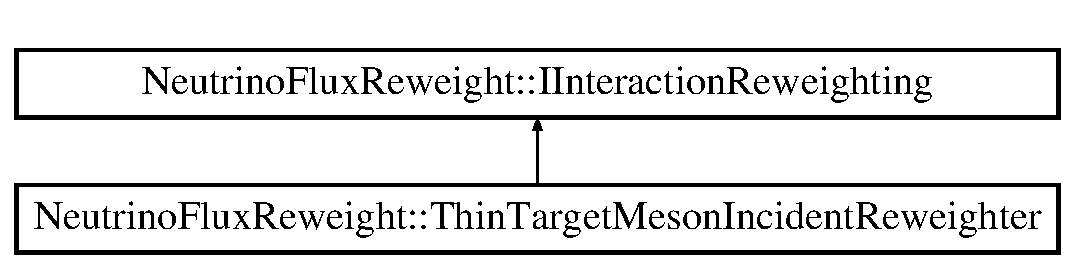
\includegraphics[height=2.000000cm]{class_neutrino_flux_reweight_1_1_thin_target_meson_incident_reweighter}
\end{center}
\end{figure}
\subsection*{Public Member Functions}
\begin{DoxyCompactItemize}
\item 
\hyperlink{class_neutrino_flux_reweight_1_1_thin_target_meson_incident_reweighter_a4f5d062846bbacf572bba8d4efba0082}{Thin\-Target\-Meson\-Incident\-Reweighter} (int iuniv, const \hyperlink{class_neutrino_flux_reweight_1_1_parameter_table}{Parameter\-Table} \&cv\-\_\-pars, const \hyperlink{class_neutrino_flux_reweight_1_1_parameter_table}{Parameter\-Table} \&univ\-\_\-pars)
\item 
virtual \hyperlink{class_neutrino_flux_reweight_1_1_thin_target_meson_incident_reweighter_a3055acaa26cbb3ca0016563410d5a58f}{$\sim$\-Thin\-Target\-Meson\-Incident\-Reweighter} ()
\item 
virtual bool \hyperlink{class_neutrino_flux_reweight_1_1_thin_target_meson_incident_reweighter_ad6974a8bf1b26e86252ee2bc1e112c5a}{can\-Reweight} (const \hyperlink{class_neutrino_flux_reweight_1_1_interaction_data}{Interaction\-Data} \&aa)
\begin{DoxyCompactList}\small\item\em can the particular instance of this class reweight this interaction? \end{DoxyCompactList}\item 
virtual double \hyperlink{class_neutrino_flux_reweight_1_1_thin_target_meson_incident_reweighter_adfb3f3e69286e74c6a9c681a0593b4d5}{calculate\-Weight} (const \hyperlink{class_neutrino_flux_reweight_1_1_interaction_data}{Interaction\-Data} \&aa)
\begin{DoxyCompactList}\small\item\em calculate a weight for this interaction given the central value parameters and the parameters for this universe. The weight is something like\-: f(cv)/f(M\-C) $\ast$ f(univ)/f(cv) where cv in this case corresponds to the best value of the parameter, given the data. If univ\-\_\-pars=cv\-\_\-pars then we are calculating a central value weight \end{DoxyCompactList}\end{DoxyCompactItemize}
\subsection*{Public Attributes}
\begin{DoxyCompactItemize}
\item 
std\-::vector$<$ float $>$ \hyperlink{class_neutrino_flux_reweight_1_1_thin_target_meson_incident_reweighter_afb51aec44c86299cc25d2b67936fdaa0}{vbin\-\_\-pip\-\_\-inc\-\_\-pip}
\item 
std\-::vector$<$ float $>$ \hyperlink{class_neutrino_flux_reweight_1_1_thin_target_meson_incident_reweighter_aaf511004916c8cde16914f776bd24567}{vbin\-\_\-pip\-\_\-inc\-\_\-pim}
\item 
std\-::vector$<$ float $>$ \hyperlink{class_neutrino_flux_reweight_1_1_thin_target_meson_incident_reweighter_a313579b46a30eab2e8181bdbb616400b}{vbin\-\_\-pip\-\_\-inc\-\_\-kap}
\item 
std\-::vector$<$ float $>$ \hyperlink{class_neutrino_flux_reweight_1_1_thin_target_meson_incident_reweighter_a4b9a6dea5fa9006465b9869f7f5a7ef4}{vbin\-\_\-pip\-\_\-inc\-\_\-kam}
\item 
std\-::vector$<$ float $>$ \hyperlink{class_neutrino_flux_reweight_1_1_thin_target_meson_incident_reweighter_a4dc56ba2cd4aefe825f48334dc9fd570}{vbin\-\_\-pip\-\_\-inc\-\_\-k0}
\item 
std\-::vector$<$ float $>$ \hyperlink{class_neutrino_flux_reweight_1_1_thin_target_meson_incident_reweighter_a094b50773eedca4a30e58067d55b61c7}{vbin\-\_\-pip\-\_\-inc\-\_\-p}
\item 
std\-::vector$<$ float $>$ \hyperlink{class_neutrino_flux_reweight_1_1_thin_target_meson_incident_reweighter_a709b2752b6bf405c479a985a136a8c5e}{vbin\-\_\-pip\-\_\-inc\-\_\-n}
\item 
std\-::vector$<$ float $>$ \hyperlink{class_neutrino_flux_reweight_1_1_thin_target_meson_incident_reweighter_a91fcf6a2aae6942bca236752fa38af15}{vbin\-\_\-pim\-\_\-inc\-\_\-pip}
\item 
std\-::vector$<$ float $>$ \hyperlink{class_neutrino_flux_reweight_1_1_thin_target_meson_incident_reweighter_ad9fb46f9b120a879ab057578902ba63e}{vbin\-\_\-pim\-\_\-inc\-\_\-pim}
\item 
std\-::vector$<$ float $>$ \hyperlink{class_neutrino_flux_reweight_1_1_thin_target_meson_incident_reweighter_adb7bd7bf69b005ef32845bf80d0dcff3}{vbin\-\_\-pim\-\_\-inc\-\_\-kap}
\item 
std\-::vector$<$ float $>$ \hyperlink{class_neutrino_flux_reweight_1_1_thin_target_meson_incident_reweighter_a1673f9e513edfa4f1435c572870d3b84}{vbin\-\_\-pim\-\_\-inc\-\_\-kam}
\item 
std\-::vector$<$ float $>$ \hyperlink{class_neutrino_flux_reweight_1_1_thin_target_meson_incident_reweighter_ad96b9c15064515154988b33c1a237743}{vbin\-\_\-pim\-\_\-inc\-\_\-k0}
\item 
std\-::vector$<$ float $>$ \hyperlink{class_neutrino_flux_reweight_1_1_thin_target_meson_incident_reweighter_a66fec429ebe5b6e00e3f015ac3796297}{vbin\-\_\-pim\-\_\-inc\-\_\-p}
\item 
std\-::vector$<$ float $>$ \hyperlink{class_neutrino_flux_reweight_1_1_thin_target_meson_incident_reweighter_a7eba845bf5fa002d9e3634318d662568}{vbin\-\_\-pim\-\_\-inc\-\_\-n}
\item 
std\-::vector$<$ float $>$ \hyperlink{class_neutrino_flux_reweight_1_1_thin_target_meson_incident_reweighter_a72f48dfba611a3737f4da6bc4302c05b}{vbin\-\_\-kap\-\_\-inc\-\_\-pip}
\item 
std\-::vector$<$ float $>$ \hyperlink{class_neutrino_flux_reweight_1_1_thin_target_meson_incident_reweighter_a244ee71b70a5e13611fe3cac77dd5848}{vbin\-\_\-kap\-\_\-inc\-\_\-pim}
\item 
std\-::vector$<$ float $>$ \hyperlink{class_neutrino_flux_reweight_1_1_thin_target_meson_incident_reweighter_a684df85cab4b7042cb79135fc7ceb6ae}{vbin\-\_\-kap\-\_\-inc\-\_\-kap}
\item 
std\-::vector$<$ float $>$ \hyperlink{class_neutrino_flux_reweight_1_1_thin_target_meson_incident_reweighter_a75572bfb96c73d133145b2aed9737be9}{vbin\-\_\-kap\-\_\-inc\-\_\-kam}
\item 
std\-::vector$<$ float $>$ \hyperlink{class_neutrino_flux_reweight_1_1_thin_target_meson_incident_reweighter_a7091af2d57521ec0ddc249424874cf75}{vbin\-\_\-kap\-\_\-inc\-\_\-k0}
\item 
std\-::vector$<$ float $>$ \hyperlink{class_neutrino_flux_reweight_1_1_thin_target_meson_incident_reweighter_af309e694aff739fbb0e3805b42fcd515}{vbin\-\_\-kap\-\_\-inc\-\_\-p}
\item 
std\-::vector$<$ float $>$ \hyperlink{class_neutrino_flux_reweight_1_1_thin_target_meson_incident_reweighter_a2922c8a50ce538b4abea1c364d6adc9b}{vbin\-\_\-kap\-\_\-inc\-\_\-n}
\item 
std\-::vector$<$ float $>$ \hyperlink{class_neutrino_flux_reweight_1_1_thin_target_meson_incident_reweighter_ac82429351c909aeaafe750d0fe4403cb}{vbin\-\_\-kam\-\_\-inc\-\_\-pip}
\item 
std\-::vector$<$ float $>$ \hyperlink{class_neutrino_flux_reweight_1_1_thin_target_meson_incident_reweighter_a8a9fa5100a6c1a2031a1263ad6ed5312}{vbin\-\_\-kam\-\_\-inc\-\_\-pim}
\item 
std\-::vector$<$ float $>$ \hyperlink{class_neutrino_flux_reweight_1_1_thin_target_meson_incident_reweighter_a5fdcae1a81d4af5da9972ec67395a113}{vbin\-\_\-kam\-\_\-inc\-\_\-kap}
\item 
std\-::vector$<$ float $>$ \hyperlink{class_neutrino_flux_reweight_1_1_thin_target_meson_incident_reweighter_a3cd983d528f4fd3603fef04084751df3}{vbin\-\_\-kam\-\_\-inc\-\_\-kam}
\item 
std\-::vector$<$ float $>$ \hyperlink{class_neutrino_flux_reweight_1_1_thin_target_meson_incident_reweighter_a613978871a5d27998977245f7f9d0b69}{vbin\-\_\-kam\-\_\-inc\-\_\-k0}
\item 
std\-::vector$<$ float $>$ \hyperlink{class_neutrino_flux_reweight_1_1_thin_target_meson_incident_reweighter_a3921cfcf4c109696542983913db1927e}{vbin\-\_\-kam\-\_\-inc\-\_\-p}
\item 
std\-::vector$<$ float $>$ \hyperlink{class_neutrino_flux_reweight_1_1_thin_target_meson_incident_reweighter_acf30f4374e9357a5c8b40ff459f4d2a8}{vbin\-\_\-kam\-\_\-inc\-\_\-n}
\item 
std\-::vector$<$ float $>$ \hyperlink{class_neutrino_flux_reweight_1_1_thin_target_meson_incident_reweighter_a468f0c6421e61b547e1c14a06e23ee81}{vbin\-\_\-k0\-\_\-inc\-\_\-pip}
\item 
std\-::vector$<$ float $>$ \hyperlink{class_neutrino_flux_reweight_1_1_thin_target_meson_incident_reweighter_a75f45bee6d5c569d86fb39fc8985c063}{vbin\-\_\-k0\-\_\-inc\-\_\-pim}
\item 
std\-::vector$<$ float $>$ \hyperlink{class_neutrino_flux_reweight_1_1_thin_target_meson_incident_reweighter_af7170b60c8ca1d198bb17cbbacea10e6}{vbin\-\_\-k0\-\_\-inc\-\_\-kap}
\item 
std\-::vector$<$ float $>$ \hyperlink{class_neutrino_flux_reweight_1_1_thin_target_meson_incident_reweighter_ad783e52b4a6206cbb7276d4d168b4807}{vbin\-\_\-k0\-\_\-inc\-\_\-kam}
\item 
std\-::vector$<$ float $>$ \hyperlink{class_neutrino_flux_reweight_1_1_thin_target_meson_incident_reweighter_a965f246458feafcee2f9931b2678efd8}{vbin\-\_\-k0\-\_\-inc\-\_\-k0}
\item 
std\-::vector$<$ float $>$ \hyperlink{class_neutrino_flux_reweight_1_1_thin_target_meson_incident_reweighter_a4504e9d8374cd8c8c631d25ceaf35a9d}{vbin\-\_\-k0\-\_\-inc\-\_\-p}
\item 
std\-::vector$<$ float $>$ \hyperlink{class_neutrino_flux_reweight_1_1_thin_target_meson_incident_reweighter_a406b7314c117edd343d2d9418b48262f}{vbin\-\_\-k0\-\_\-inc\-\_\-n}
\item 
float \hyperlink{class_neutrino_flux_reweight_1_1_thin_target_meson_incident_reweighter_af8a00936922518cafeca2199c385c3f8}{bin\-\_\-mesonleftover\-\_\-inc}
\end{DoxyCompactItemize}
\subsection*{Private Attributes}
\begin{DoxyCompactItemize}
\item 
int \hyperlink{class_neutrino_flux_reweight_1_1_thin_target_meson_incident_reweighter_aba895e921936f33c25a89daa18c1bf5d}{i\-Univ}
\item 
const \hyperlink{class_neutrino_flux_reweight_1_1_parameter_table}{Parameter\-Table} \& \hyperlink{class_neutrino_flux_reweight_1_1_thin_target_meson_incident_reweighter_a1e7d2570076d7f35a84edfd053ef7b54}{cv\-Pars}
\item 
const \hyperlink{class_neutrino_flux_reweight_1_1_parameter_table}{Parameter\-Table} \& \hyperlink{class_neutrino_flux_reweight_1_1_thin_target_meson_incident_reweighter_a04e7825e0d90c6a0315028620f2ac511}{univ\-Pars}
\end{DoxyCompactItemize}


\subsection{Detailed Description}
Reweighter of thin target meson production. 

Definition at line 19 of file Thin\-Target\-Meson\-Incident\-Reweighter.\-h.



\subsection{Constructor \& Destructor Documentation}
\hypertarget{class_neutrino_flux_reweight_1_1_thin_target_meson_incident_reweighter_a4f5d062846bbacf572bba8d4efba0082}{\index{Neutrino\-Flux\-Reweight\-::\-Thin\-Target\-Meson\-Incident\-Reweighter@{Neutrino\-Flux\-Reweight\-::\-Thin\-Target\-Meson\-Incident\-Reweighter}!Thin\-Target\-Meson\-Incident\-Reweighter@{Thin\-Target\-Meson\-Incident\-Reweighter}}
\index{Thin\-Target\-Meson\-Incident\-Reweighter@{Thin\-Target\-Meson\-Incident\-Reweighter}!NeutrinoFluxReweight::ThinTargetMesonIncidentReweighter@{Neutrino\-Flux\-Reweight\-::\-Thin\-Target\-Meson\-Incident\-Reweighter}}
\subsubsection[{Thin\-Target\-Meson\-Incident\-Reweighter}]{\setlength{\rightskip}{0pt plus 5cm}Neutrino\-Flux\-Reweight\-::\-Thin\-Target\-Meson\-Incident\-Reweighter\-::\-Thin\-Target\-Meson\-Incident\-Reweighter (
\begin{DoxyParamCaption}
\item[{int}]{iuniv, }
\item[{const {\bf Parameter\-Table} \&}]{cv\-\_\-pars, }
\item[{const {\bf Parameter\-Table} \&}]{univ\-\_\-pars}
\end{DoxyParamCaption}
)}}\label{class_neutrino_flux_reweight_1_1_thin_target_meson_incident_reweighter_a4f5d062846bbacf572bba8d4efba0082}


Definition at line 8 of file Thin\-Target\-Meson\-Incident\-Reweighter.\-cpp.


\begin{DoxyCode}
8                                                                                                            
                                          :\hyperlink{class_neutrino_flux_reweight_1_1_thin_target_meson_incident_reweighter_aba895e921936f33c25a89daa18c1bf5d}{iUniv}(iuniv),\hyperlink{class_neutrino_flux_reweight_1_1_thin_target_meson_incident_reweighter_a1e7d2570076d7f35a84edfd053ef7b54}{cvPars}(cv\_pars),
      \hyperlink{class_neutrino_flux_reweight_1_1_thin_target_meson_incident_reweighter_a04e7825e0d90c6a0315028620f2ac511}{univPars}(univ\_pars)\{
9     
10     ThinTargetBins* Thinbins =  \hyperlink{class_neutrino_flux_reweight_1_1_thin_target_bins_aeff5cf7220dd08322f5abac2cbc7ff33}{ThinTargetBins::getInstance}();
11     
12     \textcolor{comment}{//vbin\_pip\_inc\_pip.reserve(Thinbins->GetNbins\_meson\_incident());  //BHU,one}
13     \hyperlink{class_neutrino_flux_reweight_1_1_thin_target_meson_incident_reweighter_aaf511004916c8cde16914f776bd24567}{vbin\_pip\_inc\_pim}.reserve(Thinbins->GetNbins\_meson\_incident());
14     \hyperlink{class_neutrino_flux_reweight_1_1_thin_target_meson_incident_reweighter_a313579b46a30eab2e8181bdbb616400b}{vbin\_pip\_inc\_kap}.reserve(Thinbins->GetNbins\_meson\_incident());
15     \hyperlink{class_neutrino_flux_reweight_1_1_thin_target_meson_incident_reweighter_a4b9a6dea5fa9006465b9869f7f5a7ef4}{vbin\_pip\_inc\_kam}.reserve(Thinbins->GetNbins\_meson\_incident());
16     \hyperlink{class_neutrino_flux_reweight_1_1_thin_target_meson_incident_reweighter_a4dc56ba2cd4aefe825f48334dc9fd570}{vbin\_pip\_inc\_k0}.reserve(Thinbins->GetNbins\_meson\_incident());
17     \hyperlink{class_neutrino_flux_reweight_1_1_thin_target_meson_incident_reweighter_a094b50773eedca4a30e58067d55b61c7}{vbin\_pip\_inc\_p}.reserve(Thinbins->GetNbins\_meson\_incident());
18     \hyperlink{class_neutrino_flux_reweight_1_1_thin_target_meson_incident_reweighter_a709b2752b6bf405c479a985a136a8c5e}{vbin\_pip\_inc\_n}.reserve(Thinbins->GetNbins\_meson\_incident());
19     \hyperlink{class_neutrino_flux_reweight_1_1_thin_target_meson_incident_reweighter_a91fcf6a2aae6942bca236752fa38af15}{vbin\_pim\_inc\_pip}.reserve(Thinbins->GetNbins\_meson\_incident());
20     \hyperlink{class_neutrino_flux_reweight_1_1_thin_target_meson_incident_reweighter_ad9fb46f9b120a879ab057578902ba63e}{vbin\_pim\_inc\_pim}.reserve(Thinbins->GetNbins\_meson\_incident());
21     \hyperlink{class_neutrino_flux_reweight_1_1_thin_target_meson_incident_reweighter_adb7bd7bf69b005ef32845bf80d0dcff3}{vbin\_pim\_inc\_kap}.reserve(Thinbins->GetNbins\_meson\_incident());
22     \hyperlink{class_neutrino_flux_reweight_1_1_thin_target_meson_incident_reweighter_a1673f9e513edfa4f1435c572870d3b84}{vbin\_pim\_inc\_kam}.reserve(Thinbins->GetNbins\_meson\_incident());
23     \hyperlink{class_neutrino_flux_reweight_1_1_thin_target_meson_incident_reweighter_ad96b9c15064515154988b33c1a237743}{vbin\_pim\_inc\_k0}.reserve(Thinbins->GetNbins\_meson\_incident());
24     \hyperlink{class_neutrino_flux_reweight_1_1_thin_target_meson_incident_reweighter_a66fec429ebe5b6e00e3f015ac3796297}{vbin\_pim\_inc\_p}.reserve(Thinbins->GetNbins\_meson\_incident());
25     \hyperlink{class_neutrino_flux_reweight_1_1_thin_target_meson_incident_reweighter_a7eba845bf5fa002d9e3634318d662568}{vbin\_pim\_inc\_n}.reserve(Thinbins->GetNbins\_meson\_incident());
26     \hyperlink{class_neutrino_flux_reweight_1_1_thin_target_meson_incident_reweighter_a72f48dfba611a3737f4da6bc4302c05b}{vbin\_kap\_inc\_pip}.reserve(Thinbins->GetNbins\_meson\_incident());
27     \hyperlink{class_neutrino_flux_reweight_1_1_thin_target_meson_incident_reweighter_a244ee71b70a5e13611fe3cac77dd5848}{vbin\_kap\_inc\_pim}.reserve(Thinbins->GetNbins\_meson\_incident());
28     \hyperlink{class_neutrino_flux_reweight_1_1_thin_target_meson_incident_reweighter_a684df85cab4b7042cb79135fc7ceb6ae}{vbin\_kap\_inc\_kap}.reserve(Thinbins->GetNbins\_meson\_incident());
29     \hyperlink{class_neutrino_flux_reweight_1_1_thin_target_meson_incident_reweighter_a75572bfb96c73d133145b2aed9737be9}{vbin\_kap\_inc\_kam}.reserve(Thinbins->GetNbins\_meson\_incident());
30     \hyperlink{class_neutrino_flux_reweight_1_1_thin_target_meson_incident_reweighter_a7091af2d57521ec0ddc249424874cf75}{vbin\_kap\_inc\_k0}.reserve(Thinbins->GetNbins\_meson\_incident());
31     \hyperlink{class_neutrino_flux_reweight_1_1_thin_target_meson_incident_reweighter_af309e694aff739fbb0e3805b42fcd515}{vbin\_kap\_inc\_p}.reserve(Thinbins->GetNbins\_meson\_incident());
32     \hyperlink{class_neutrino_flux_reweight_1_1_thin_target_meson_incident_reweighter_a2922c8a50ce538b4abea1c364d6adc9b}{vbin\_kap\_inc\_n}.reserve(Thinbins->GetNbins\_meson\_incident());
33     \hyperlink{class_neutrino_flux_reweight_1_1_thin_target_meson_incident_reweighter_ac82429351c909aeaafe750d0fe4403cb}{vbin\_kam\_inc\_pip}.reserve(Thinbins->GetNbins\_meson\_incident());
34     \hyperlink{class_neutrino_flux_reweight_1_1_thin_target_meson_incident_reweighter_a8a9fa5100a6c1a2031a1263ad6ed5312}{vbin\_kam\_inc\_pim}.reserve(Thinbins->GetNbins\_meson\_incident());
35     \hyperlink{class_neutrino_flux_reweight_1_1_thin_target_meson_incident_reweighter_a5fdcae1a81d4af5da9972ec67395a113}{vbin\_kam\_inc\_kap}.reserve(Thinbins->GetNbins\_meson\_incident());
36     \hyperlink{class_neutrino_flux_reweight_1_1_thin_target_meson_incident_reweighter_a3cd983d528f4fd3603fef04084751df3}{vbin\_kam\_inc\_kam}.reserve(Thinbins->GetNbins\_meson\_incident());
37     \hyperlink{class_neutrino_flux_reweight_1_1_thin_target_meson_incident_reweighter_a613978871a5d27998977245f7f9d0b69}{vbin\_kam\_inc\_k0}.reserve(Thinbins->GetNbins\_meson\_incident());
38     \hyperlink{class_neutrino_flux_reweight_1_1_thin_target_meson_incident_reweighter_a3921cfcf4c109696542983913db1927e}{vbin\_kam\_inc\_p}.reserve(Thinbins->GetNbins\_meson\_incident());
39     \hyperlink{class_neutrino_flux_reweight_1_1_thin_target_meson_incident_reweighter_acf30f4374e9357a5c8b40ff459f4d2a8}{vbin\_kam\_inc\_n}.reserve(Thinbins->GetNbins\_meson\_incident());
40     \hyperlink{class_neutrino_flux_reweight_1_1_thin_target_meson_incident_reweighter_a468f0c6421e61b547e1c14a06e23ee81}{vbin\_k0\_inc\_pip}.reserve(Thinbins->GetNbins\_meson\_incident());
41     \hyperlink{class_neutrino_flux_reweight_1_1_thin_target_meson_incident_reweighter_a75f45bee6d5c569d86fb39fc8985c063}{vbin\_k0\_inc\_pim}.reserve(Thinbins->GetNbins\_meson\_incident());
42     \hyperlink{class_neutrino_flux_reweight_1_1_thin_target_meson_incident_reweighter_af7170b60c8ca1d198bb17cbbacea10e6}{vbin\_k0\_inc\_kap}.reserve(Thinbins->GetNbins\_meson\_incident());
43     \hyperlink{class_neutrino_flux_reweight_1_1_thin_target_meson_incident_reweighter_ad783e52b4a6206cbb7276d4d168b4807}{vbin\_k0\_inc\_kam}.reserve(Thinbins->GetNbins\_meson\_incident());
44     \hyperlink{class_neutrino_flux_reweight_1_1_thin_target_meson_incident_reweighter_a965f246458feafcee2f9931b2678efd8}{vbin\_k0\_inc\_k0}.reserve(Thinbins->GetNbins\_meson\_incident());
45     \hyperlink{class_neutrino_flux_reweight_1_1_thin_target_meson_incident_reweighter_a4504e9d8374cd8c8c631d25ceaf35a9d}{vbin\_k0\_inc\_p}.reserve(Thinbins->GetNbins\_meson\_incident());
46     \hyperlink{class_neutrino_flux_reweight_1_1_thin_target_meson_incident_reweighter_a406b7314c117edd343d2d9418b48262f}{vbin\_k0\_inc\_n}.reserve(Thinbins->GetNbins\_meson\_incident());
47 
48     \textcolor{comment}{// const boost::interprocess::flat\_map<std::string, double>& cv\_table   = cvPars.getMap();}
49     \textcolor{comment}{// const boost::interprocess::flat\_map<std::string, double>& univ\_table = univPars.getMap();}
50     \textcolor{keywordtype}{char} namepar[100];
51 
52     \textcolor{comment}{//meson left over:}
53     sprintf(namepar,\textcolor{stringliteral}{"ThinTarget\_mesonleftover\_incident\_%d"},0);
54     \textcolor{keywordtype}{double} dataval = \hyperlink{class_neutrino_flux_reweight_1_1_thin_target_meson_incident_reweighter_a04e7825e0d90c6a0315028620f2ac511}{univPars}.\hyperlink{class_neutrino_flux_reweight_1_1_parameter_table_acb7dc8335b65b116f6092f2fa57ca5ed}{getParameterValue}(std::string(namepar));
55     \hyperlink{class_neutrino_flux_reweight_1_1_thin_target_meson_incident_reweighter_af8a00936922518cafeca2199c385c3f8}{bin\_mesonleftover\_inc} = dataval;
56     
57     \textcolor{comment}{//5 incident particles, 7 produced particles:}
58     \textcolor{keyword}{const} \textcolor{keywordtype}{char}* cinc[5] = \{\textcolor{stringliteral}{"pip"},\textcolor{stringliteral}{"pim"},\textcolor{stringliteral}{"kap"},\textcolor{stringliteral}{"kam"},\textcolor{stringliteral}{"k0"}\};
59     \textcolor{keyword}{const} \textcolor{keywordtype}{char}* cpro[7] = \{\textcolor{stringliteral}{"pip"},\textcolor{stringliteral}{"pim"},\textcolor{stringliteral}{"kap"},\textcolor{stringliteral}{"kam"},\textcolor{stringliteral}{"k0"},\textcolor{stringliteral}{"p"},\textcolor{stringliteral}{"n"}\};
60     
61     \textcolor{keywordflow}{for}(\textcolor{keywordtype}{int} ii=0;ii<5;ii++)\{
62       \textcolor{keywordflow}{for}(\textcolor{keywordtype}{int} jj=0;jj<7;jj++)\{
63         \textcolor{keywordflow}{for}(\textcolor{keywordtype}{int} kk=0;kk<4;kk++)\{
64           
65           sprintf(namepar,\textcolor{stringliteral}{"ThinTarget\_%s\_incident\_%s\_%d"},cinc[ii],cpro[jj],kk);
66           dataval = \hyperlink{class_neutrino_flux_reweight_1_1_thin_target_meson_incident_reweighter_a04e7825e0d90c6a0315028620f2ac511}{univPars}.\hyperlink{class_neutrino_flux_reweight_1_1_parameter_table_acb7dc8335b65b116f6092f2fa57ca5ed}{getParameterValue}(std::string(namepar));
67          \textcolor{comment}{//if(ii==0 && jj==0)vbin\_pip\_inc\_pip.push\_back(dataval);   //BHU. two}
68           \textcolor{keywordflow}{if}(ii==0 && jj==1)\hyperlink{class_neutrino_flux_reweight_1_1_thin_target_meson_incident_reweighter_aaf511004916c8cde16914f776bd24567}{vbin\_pip\_inc\_pim}.push\_back(dataval);
69           \textcolor{keywordflow}{if}(ii==0 && jj==2)\hyperlink{class_neutrino_flux_reweight_1_1_thin_target_meson_incident_reweighter_a313579b46a30eab2e8181bdbb616400b}{vbin\_pip\_inc\_kap}.push\_back(dataval);
70           \textcolor{keywordflow}{if}(ii==0 && jj==3)\hyperlink{class_neutrino_flux_reweight_1_1_thin_target_meson_incident_reweighter_a4b9a6dea5fa9006465b9869f7f5a7ef4}{vbin\_pip\_inc\_kam}.push\_back(dataval);
71           \textcolor{keywordflow}{if}(ii==0 && jj==4)\hyperlink{class_neutrino_flux_reweight_1_1_thin_target_meson_incident_reweighter_a4dc56ba2cd4aefe825f48334dc9fd570}{vbin\_pip\_inc\_k0}.push\_back(dataval);
72           \textcolor{keywordflow}{if}(ii==0 && jj==5)\hyperlink{class_neutrino_flux_reweight_1_1_thin_target_meson_incident_reweighter_a094b50773eedca4a30e58067d55b61c7}{vbin\_pip\_inc\_p}.push\_back(dataval);
73           \textcolor{keywordflow}{if}(ii==0 && jj==6)\hyperlink{class_neutrino_flux_reweight_1_1_thin_target_meson_incident_reweighter_a709b2752b6bf405c479a985a136a8c5e}{vbin\_pip\_inc\_n}.push\_back(dataval);
74           \textcolor{keywordflow}{if}(ii==1 && jj==0)\hyperlink{class_neutrino_flux_reweight_1_1_thin_target_meson_incident_reweighter_a91fcf6a2aae6942bca236752fa38af15}{vbin\_pim\_inc\_pip}.push\_back(dataval);
75           \textcolor{keywordflow}{if}(ii==1 && jj==1)\hyperlink{class_neutrino_flux_reweight_1_1_thin_target_meson_incident_reweighter_ad9fb46f9b120a879ab057578902ba63e}{vbin\_pim\_inc\_pim}.push\_back(dataval);
76           \textcolor{keywordflow}{if}(ii==1 && jj==2)\hyperlink{class_neutrino_flux_reweight_1_1_thin_target_meson_incident_reweighter_adb7bd7bf69b005ef32845bf80d0dcff3}{vbin\_pim\_inc\_kap}.push\_back(dataval);
77           \textcolor{keywordflow}{if}(ii==1 && jj==3)\hyperlink{class_neutrino_flux_reweight_1_1_thin_target_meson_incident_reweighter_a1673f9e513edfa4f1435c572870d3b84}{vbin\_pim\_inc\_kam}.push\_back(dataval);
78           \textcolor{keywordflow}{if}(ii==1 && jj==4)\hyperlink{class_neutrino_flux_reweight_1_1_thin_target_meson_incident_reweighter_ad96b9c15064515154988b33c1a237743}{vbin\_pim\_inc\_k0}.push\_back(dataval);
79           \textcolor{keywordflow}{if}(ii==1 && jj==5)\hyperlink{class_neutrino_flux_reweight_1_1_thin_target_meson_incident_reweighter_a66fec429ebe5b6e00e3f015ac3796297}{vbin\_pim\_inc\_p}.push\_back(dataval);
80           \textcolor{keywordflow}{if}(ii==1 && jj==6)\hyperlink{class_neutrino_flux_reweight_1_1_thin_target_meson_incident_reweighter_a7eba845bf5fa002d9e3634318d662568}{vbin\_pim\_inc\_n}.push\_back(dataval);
81           \textcolor{keywordflow}{if}(ii==2 && jj==0)\hyperlink{class_neutrino_flux_reweight_1_1_thin_target_meson_incident_reweighter_a72f48dfba611a3737f4da6bc4302c05b}{vbin\_kap\_inc\_pip}.push\_back(dataval);
82           \textcolor{keywordflow}{if}(ii==2 && jj==1)\hyperlink{class_neutrino_flux_reweight_1_1_thin_target_meson_incident_reweighter_a244ee71b70a5e13611fe3cac77dd5848}{vbin\_kap\_inc\_pim}.push\_back(dataval);
83           \textcolor{keywordflow}{if}(ii==2 && jj==2)\hyperlink{class_neutrino_flux_reweight_1_1_thin_target_meson_incident_reweighter_a684df85cab4b7042cb79135fc7ceb6ae}{vbin\_kap\_inc\_kap}.push\_back(dataval);
84           \textcolor{keywordflow}{if}(ii==2 && jj==3)\hyperlink{class_neutrino_flux_reweight_1_1_thin_target_meson_incident_reweighter_a75572bfb96c73d133145b2aed9737be9}{vbin\_kap\_inc\_kam}.push\_back(dataval);
85           \textcolor{keywordflow}{if}(ii==2 && jj==4)\hyperlink{class_neutrino_flux_reweight_1_1_thin_target_meson_incident_reweighter_a7091af2d57521ec0ddc249424874cf75}{vbin\_kap\_inc\_k0}.push\_back(dataval);
86           \textcolor{keywordflow}{if}(ii==2 && jj==5)\hyperlink{class_neutrino_flux_reweight_1_1_thin_target_meson_incident_reweighter_af309e694aff739fbb0e3805b42fcd515}{vbin\_kap\_inc\_p}.push\_back(dataval);
87           \textcolor{keywordflow}{if}(ii==2 && jj==6)\hyperlink{class_neutrino_flux_reweight_1_1_thin_target_meson_incident_reweighter_a2922c8a50ce538b4abea1c364d6adc9b}{vbin\_kap\_inc\_n}.push\_back(dataval);
88           \textcolor{keywordflow}{if}(ii==3 && jj==0)\hyperlink{class_neutrino_flux_reweight_1_1_thin_target_meson_incident_reweighter_ac82429351c909aeaafe750d0fe4403cb}{vbin\_kam\_inc\_pip}.push\_back(dataval);
89           \textcolor{keywordflow}{if}(ii==3 && jj==1)\hyperlink{class_neutrino_flux_reweight_1_1_thin_target_meson_incident_reweighter_a8a9fa5100a6c1a2031a1263ad6ed5312}{vbin\_kam\_inc\_pim}.push\_back(dataval);
90           \textcolor{keywordflow}{if}(ii==3 && jj==2)\hyperlink{class_neutrino_flux_reweight_1_1_thin_target_meson_incident_reweighter_a5fdcae1a81d4af5da9972ec67395a113}{vbin\_kam\_inc\_kap}.push\_back(dataval);
91           \textcolor{keywordflow}{if}(ii==3 && jj==3)\hyperlink{class_neutrino_flux_reweight_1_1_thin_target_meson_incident_reweighter_a3cd983d528f4fd3603fef04084751df3}{vbin\_kam\_inc\_kam}.push\_back(dataval);
92           \textcolor{keywordflow}{if}(ii==3 && jj==4)\hyperlink{class_neutrino_flux_reweight_1_1_thin_target_meson_incident_reweighter_a613978871a5d27998977245f7f9d0b69}{vbin\_kam\_inc\_k0}.push\_back(dataval);
93           \textcolor{keywordflow}{if}(ii==3 && jj==5)\hyperlink{class_neutrino_flux_reweight_1_1_thin_target_meson_incident_reweighter_a3921cfcf4c109696542983913db1927e}{vbin\_kam\_inc\_p}.push\_back(dataval);
94           \textcolor{keywordflow}{if}(ii==3 && jj==6)\hyperlink{class_neutrino_flux_reweight_1_1_thin_target_meson_incident_reweighter_acf30f4374e9357a5c8b40ff459f4d2a8}{vbin\_kam\_inc\_n}.push\_back(dataval);
95           \textcolor{keywordflow}{if}(ii==4 && jj==0)\hyperlink{class_neutrino_flux_reweight_1_1_thin_target_meson_incident_reweighter_a468f0c6421e61b547e1c14a06e23ee81}{vbin\_k0\_inc\_pip}.push\_back(dataval);
96           \textcolor{keywordflow}{if}(ii==4 && jj==1)\hyperlink{class_neutrino_flux_reweight_1_1_thin_target_meson_incident_reweighter_a75f45bee6d5c569d86fb39fc8985c063}{vbin\_k0\_inc\_pim}.push\_back(dataval);
97           \textcolor{keywordflow}{if}(ii==4 && jj==2)\hyperlink{class_neutrino_flux_reweight_1_1_thin_target_meson_incident_reweighter_af7170b60c8ca1d198bb17cbbacea10e6}{vbin\_k0\_inc\_kap}.push\_back(dataval);
98           \textcolor{keywordflow}{if}(ii==4 && jj==3)\hyperlink{class_neutrino_flux_reweight_1_1_thin_target_meson_incident_reweighter_ad783e52b4a6206cbb7276d4d168b4807}{vbin\_k0\_inc\_kam}.push\_back(dataval);
99           \textcolor{keywordflow}{if}(ii==4 && jj==4)\hyperlink{class_neutrino_flux_reweight_1_1_thin_target_meson_incident_reweighter_a965f246458feafcee2f9931b2678efd8}{vbin\_k0\_inc\_k0}.push\_back(dataval);
100           \textcolor{keywordflow}{if}(ii==4 && jj==5)\hyperlink{class_neutrino_flux_reweight_1_1_thin_target_meson_incident_reweighter_a4504e9d8374cd8c8c631d25ceaf35a9d}{vbin\_k0\_inc\_p}.push\_back(dataval);
101           \textcolor{keywordflow}{if}(ii==4 && jj==6)\hyperlink{class_neutrino_flux_reweight_1_1_thin_target_meson_incident_reweighter_a406b7314c117edd343d2d9418b48262f}{vbin\_k0\_inc\_n}.push\_back(dataval);
102         \}
103       \}
104     \}
105   \}
\end{DoxyCode}
\hypertarget{class_neutrino_flux_reweight_1_1_thin_target_meson_incident_reweighter_a3055acaa26cbb3ca0016563410d5a58f}{\index{Neutrino\-Flux\-Reweight\-::\-Thin\-Target\-Meson\-Incident\-Reweighter@{Neutrino\-Flux\-Reweight\-::\-Thin\-Target\-Meson\-Incident\-Reweighter}!$\sim$\-Thin\-Target\-Meson\-Incident\-Reweighter@{$\sim$\-Thin\-Target\-Meson\-Incident\-Reweighter}}
\index{$\sim$\-Thin\-Target\-Meson\-Incident\-Reweighter@{$\sim$\-Thin\-Target\-Meson\-Incident\-Reweighter}!NeutrinoFluxReweight::ThinTargetMesonIncidentReweighter@{Neutrino\-Flux\-Reweight\-::\-Thin\-Target\-Meson\-Incident\-Reweighter}}
\subsubsection[{$\sim$\-Thin\-Target\-Meson\-Incident\-Reweighter}]{\setlength{\rightskip}{0pt plus 5cm}Neutrino\-Flux\-Reweight\-::\-Thin\-Target\-Meson\-Incident\-Reweighter\-::$\sim$\-Thin\-Target\-Meson\-Incident\-Reweighter (
\begin{DoxyParamCaption}
{}
\end{DoxyParamCaption}
)\hspace{0.3cm}{\ttfamily [virtual]}}}\label{class_neutrino_flux_reweight_1_1_thin_target_meson_incident_reweighter_a3055acaa26cbb3ca0016563410d5a58f}


Definition at line 107 of file Thin\-Target\-Meson\-Incident\-Reweighter.\-cpp.


\begin{DoxyCode}
107                                                                        \{
108     
109   \}
\end{DoxyCode}


\subsection{Member Function Documentation}
\hypertarget{class_neutrino_flux_reweight_1_1_thin_target_meson_incident_reweighter_adfb3f3e69286e74c6a9c681a0593b4d5}{\index{Neutrino\-Flux\-Reweight\-::\-Thin\-Target\-Meson\-Incident\-Reweighter@{Neutrino\-Flux\-Reweight\-::\-Thin\-Target\-Meson\-Incident\-Reweighter}!calculate\-Weight@{calculate\-Weight}}
\index{calculate\-Weight@{calculate\-Weight}!NeutrinoFluxReweight::ThinTargetMesonIncidentReweighter@{Neutrino\-Flux\-Reweight\-::\-Thin\-Target\-Meson\-Incident\-Reweighter}}
\subsubsection[{calculate\-Weight}]{\setlength{\rightskip}{0pt plus 5cm}double Neutrino\-Flux\-Reweight\-::\-Thin\-Target\-Meson\-Incident\-Reweighter\-::calculate\-Weight (
\begin{DoxyParamCaption}
\item[{const {\bf Interaction\-Data} \&}]{inter\-\_\-data}
\end{DoxyParamCaption}
)\hspace{0.3cm}{\ttfamily [virtual]}}}\label{class_neutrino_flux_reweight_1_1_thin_target_meson_incident_reweighter_adfb3f3e69286e74c6a9c681a0593b4d5}


calculate a weight for this interaction given the central value parameters and the parameters for this universe. The weight is something like\-: f(cv)/f(M\-C) $\ast$ f(univ)/f(cv) where cv in this case corresponds to the best value of the parameter, given the data. If univ\-\_\-pars=cv\-\_\-pars then we are calculating a central value weight 



Implements \hyperlink{class_neutrino_flux_reweight_1_1_i_interaction_reweighting_a49b0d73e778411d629205d23575703c3}{Neutrino\-Flux\-Reweight\-::\-I\-Interaction\-Reweighting}.



Definition at line 133 of file Thin\-Target\-Meson\-Incident\-Reweighter.\-cpp.


\begin{DoxyCode}
133                                                                                     \{
134 
135     \textcolor{keywordtype}{double} wgt = 1.0;
136 
137     \textcolor{keywordtype}{bool} right\_inc = aa.Inc\_pdg == 211 || aa.Inc\_pdg == -211 || aa.Inc\_pdg == 321 || aa.Inc\_pdg == -321 || 
      aa.Inc\_pdg == 130 || aa.Inc\_pdg == 310;
138     \textcolor{keywordtype}{bool} right\_prod = aa.Prod\_pdg == 211 || aa.Prod\_pdg == -211 || aa.Prod\_pdg == 321 || aa.Prod\_pdg == -
      321 || aa.Prod\_pdg == 130 || aa.Prod\_pdg == 310 || aa.Prod\_pdg == 2212 || aa.Prod\_pdg == 2112;
139     ThinTargetBins*  Thinbins =  \hyperlink{class_neutrino_flux_reweight_1_1_thin_target_bins_aeff5cf7220dd08322f5abac2cbc7ff33}{ThinTargetBins::getInstance}();
140     \textcolor{keywordtype}{int} bin      = Thinbins->meson\_inc\_BinID(aa.xF,aa.Pt,aa.Prod\_pdg);
141     \textcolor{keywordtype}{bool} is\_mesoninc = (aa.Inc\_pdg >99 && aa.Inc\_pdg < 1000) || (aa.Inc\_pdg <-99 && aa.Inc\_pdg > -1000);
142     \textcolor{keywordflow}{if}(bin>=0 && right\_inc && right\_prod)\{
143 
144       \textcolor{keywordflow}{if}(aa.Inc\_pdg == 211)\{
145         \textcolor{comment}{//if(aa.Prod\_pdg == 211) wgt = vbin\_pip\_inc\_pip[bin];      //BHU,three}
146         \textcolor{keywordflow}{if}(aa.Prod\_pdg ==-211) wgt = \hyperlink{class_neutrino_flux_reweight_1_1_thin_target_meson_incident_reweighter_aaf511004916c8cde16914f776bd24567}{vbin\_pip\_inc\_pim}[bin];
147         \textcolor{keywordflow}{if}(aa.Prod\_pdg == 321) wgt = \hyperlink{class_neutrino_flux_reweight_1_1_thin_target_meson_incident_reweighter_a313579b46a30eab2e8181bdbb616400b}{vbin\_pip\_inc\_kap}[bin];
148         \textcolor{keywordflow}{if}(aa.Prod\_pdg ==-321) wgt = \hyperlink{class_neutrino_flux_reweight_1_1_thin_target_meson_incident_reweighter_a4b9a6dea5fa9006465b9869f7f5a7ef4}{vbin\_pip\_inc\_kam}[bin];
149         \textcolor{keywordflow}{if}(aa.Prod\_pdg ==130 || aa.Prod\_pdg ==310) wgt = \hyperlink{class_neutrino_flux_reweight_1_1_thin_target_meson_incident_reweighter_a4dc56ba2cd4aefe825f48334dc9fd570}{vbin\_pip\_inc\_k0}[bin];
150         \textcolor{keywordflow}{if}(aa.Prod\_pdg ==2212) wgt = \hyperlink{class_neutrino_flux_reweight_1_1_thin_target_meson_incident_reweighter_a094b50773eedca4a30e58067d55b61c7}{vbin\_pip\_inc\_p}[bin];
151         \textcolor{keywordflow}{if}(aa.Prod\_pdg ==2112) wgt = \hyperlink{class_neutrino_flux_reweight_1_1_thin_target_meson_incident_reweighter_a709b2752b6bf405c479a985a136a8c5e}{vbin\_pip\_inc\_n}[bin]; 
152       \}
153       \textcolor{keywordflow}{else} \textcolor{keywordflow}{if}(aa.Inc\_pdg ==-211)\{
154         \textcolor{keywordflow}{if}(aa.Prod\_pdg == 211) wgt = \hyperlink{class_neutrino_flux_reweight_1_1_thin_target_meson_incident_reweighter_a91fcf6a2aae6942bca236752fa38af15}{vbin\_pim\_inc\_pip}[bin];
155         \textcolor{keywordflow}{if}(aa.Prod\_pdg ==-211) wgt = \hyperlink{class_neutrino_flux_reweight_1_1_thin_target_meson_incident_reweighter_ad9fb46f9b120a879ab057578902ba63e}{vbin\_pim\_inc\_pim}[bin];
156         \textcolor{keywordflow}{if}(aa.Prod\_pdg == 321) wgt = \hyperlink{class_neutrino_flux_reweight_1_1_thin_target_meson_incident_reweighter_adb7bd7bf69b005ef32845bf80d0dcff3}{vbin\_pim\_inc\_kap}[bin];
157         \textcolor{keywordflow}{if}(aa.Prod\_pdg ==-321) wgt = \hyperlink{class_neutrino_flux_reweight_1_1_thin_target_meson_incident_reweighter_a1673f9e513edfa4f1435c572870d3b84}{vbin\_pim\_inc\_kam}[bin];
158         \textcolor{keywordflow}{if}(aa.Prod\_pdg ==130 || aa.Prod\_pdg ==310) wgt = \hyperlink{class_neutrino_flux_reweight_1_1_thin_target_meson_incident_reweighter_ad96b9c15064515154988b33c1a237743}{vbin\_pim\_inc\_k0}[bin];
159         \textcolor{keywordflow}{if}(aa.Prod\_pdg ==2212) wgt = \hyperlink{class_neutrino_flux_reweight_1_1_thin_target_meson_incident_reweighter_a66fec429ebe5b6e00e3f015ac3796297}{vbin\_pim\_inc\_p}[bin];
160         \textcolor{keywordflow}{if}(aa.Prod\_pdg ==2112) wgt = \hyperlink{class_neutrino_flux_reweight_1_1_thin_target_meson_incident_reweighter_a7eba845bf5fa002d9e3634318d662568}{vbin\_pim\_inc\_n}[bin]; 
161       \}
162       \textcolor{keywordflow}{else} \textcolor{keywordflow}{if}(aa.Inc\_pdg == 321)\{
163         \textcolor{keywordflow}{if}(aa.Prod\_pdg == 211) wgt = \hyperlink{class_neutrino_flux_reweight_1_1_thin_target_meson_incident_reweighter_a72f48dfba611a3737f4da6bc4302c05b}{vbin\_kap\_inc\_pip}[bin];
164         \textcolor{keywordflow}{if}(aa.Prod\_pdg ==-211) wgt = \hyperlink{class_neutrino_flux_reweight_1_1_thin_target_meson_incident_reweighter_a244ee71b70a5e13611fe3cac77dd5848}{vbin\_kap\_inc\_pim}[bin];
165         \textcolor{keywordflow}{if}(aa.Prod\_pdg == 321) wgt = \hyperlink{class_neutrino_flux_reweight_1_1_thin_target_meson_incident_reweighter_a684df85cab4b7042cb79135fc7ceb6ae}{vbin\_kap\_inc\_kap}[bin];
166         \textcolor{keywordflow}{if}(aa.Prod\_pdg ==-321) wgt = \hyperlink{class_neutrino_flux_reweight_1_1_thin_target_meson_incident_reweighter_a75572bfb96c73d133145b2aed9737be9}{vbin\_kap\_inc\_kam}[bin];
167         \textcolor{keywordflow}{if}(aa.Prod\_pdg ==130 || aa.Prod\_pdg ==310) wgt = \hyperlink{class_neutrino_flux_reweight_1_1_thin_target_meson_incident_reweighter_a7091af2d57521ec0ddc249424874cf75}{vbin\_kap\_inc\_k0}[bin];
168         \textcolor{keywordflow}{if}(aa.Prod\_pdg ==2212) wgt = \hyperlink{class_neutrino_flux_reweight_1_1_thin_target_meson_incident_reweighter_af309e694aff739fbb0e3805b42fcd515}{vbin\_kap\_inc\_p}[bin];
169         \textcolor{keywordflow}{if}(aa.Prod\_pdg ==2112) wgt = \hyperlink{class_neutrino_flux_reweight_1_1_thin_target_meson_incident_reweighter_a2922c8a50ce538b4abea1c364d6adc9b}{vbin\_kap\_inc\_n}[bin]; 
170       \}
171       \textcolor{keywordflow}{else} \textcolor{keywordflow}{if}(aa.Inc\_pdg ==-321)\{
172         \textcolor{keywordflow}{if}(aa.Prod\_pdg == 211) wgt = \hyperlink{class_neutrino_flux_reweight_1_1_thin_target_meson_incident_reweighter_ac82429351c909aeaafe750d0fe4403cb}{vbin\_kam\_inc\_pip}[bin];
173         \textcolor{keywordflow}{if}(aa.Prod\_pdg ==-211) wgt = \hyperlink{class_neutrino_flux_reweight_1_1_thin_target_meson_incident_reweighter_a8a9fa5100a6c1a2031a1263ad6ed5312}{vbin\_kam\_inc\_pim}[bin];
174         \textcolor{keywordflow}{if}(aa.Prod\_pdg == 321) wgt = \hyperlink{class_neutrino_flux_reweight_1_1_thin_target_meson_incident_reweighter_a5fdcae1a81d4af5da9972ec67395a113}{vbin\_kam\_inc\_kap}[bin];
175         \textcolor{keywordflow}{if}(aa.Prod\_pdg ==-321) wgt = \hyperlink{class_neutrino_flux_reweight_1_1_thin_target_meson_incident_reweighter_a3cd983d528f4fd3603fef04084751df3}{vbin\_kam\_inc\_kam}[bin];
176         \textcolor{keywordflow}{if}(aa.Prod\_pdg ==130 || aa.Prod\_pdg ==310) wgt = \hyperlink{class_neutrino_flux_reweight_1_1_thin_target_meson_incident_reweighter_a613978871a5d27998977245f7f9d0b69}{vbin\_kam\_inc\_k0}[bin];
177         \textcolor{keywordflow}{if}(aa.Prod\_pdg ==2212) wgt = \hyperlink{class_neutrino_flux_reweight_1_1_thin_target_meson_incident_reweighter_a3921cfcf4c109696542983913db1927e}{vbin\_kam\_inc\_p}[bin];
178         \textcolor{keywordflow}{if}(aa.Prod\_pdg ==2112) wgt = \hyperlink{class_neutrino_flux_reweight_1_1_thin_target_meson_incident_reweighter_acf30f4374e9357a5c8b40ff459f4d2a8}{vbin\_kam\_inc\_n}[bin]; 
179       \}
180       \textcolor{keywordflow}{else} \textcolor{keywordflow}{if}(aa.Inc\_pdg == 130 || aa.Inc\_pdg == 310)\{
181         \textcolor{keywordflow}{if}(aa.Prod\_pdg == 211) wgt = \hyperlink{class_neutrino_flux_reweight_1_1_thin_target_meson_incident_reweighter_a468f0c6421e61b547e1c14a06e23ee81}{vbin\_k0\_inc\_pip}[bin];
182         \textcolor{keywordflow}{if}(aa.Prod\_pdg ==-211) wgt = \hyperlink{class_neutrino_flux_reweight_1_1_thin_target_meson_incident_reweighter_a75f45bee6d5c569d86fb39fc8985c063}{vbin\_k0\_inc\_pim}[bin];
183         \textcolor{keywordflow}{if}(aa.Prod\_pdg == 321) wgt = \hyperlink{class_neutrino_flux_reweight_1_1_thin_target_meson_incident_reweighter_af7170b60c8ca1d198bb17cbbacea10e6}{vbin\_k0\_inc\_kap}[bin];
184         \textcolor{keywordflow}{if}(aa.Prod\_pdg ==-321) wgt = \hyperlink{class_neutrino_flux_reweight_1_1_thin_target_meson_incident_reweighter_ad783e52b4a6206cbb7276d4d168b4807}{vbin\_k0\_inc\_kam}[bin];
185         \textcolor{keywordflow}{if}(aa.Prod\_pdg ==130 || aa.Prod\_pdg ==310) wgt = \hyperlink{class_neutrino_flux_reweight_1_1_thin_target_meson_incident_reweighter_a965f246458feafcee2f9931b2678efd8}{vbin\_k0\_inc\_k0}[bin];
186         \textcolor{keywordflow}{if}(aa.Prod\_pdg ==2212) wgt = \hyperlink{class_neutrino_flux_reweight_1_1_thin_target_meson_incident_reweighter_a4504e9d8374cd8c8c631d25ceaf35a9d}{vbin\_k0\_inc\_p}[bin];
187         \textcolor{keywordflow}{if}(aa.Prod\_pdg ==2112) wgt = \hyperlink{class_neutrino_flux_reweight_1_1_thin_target_meson_incident_reweighter_a406b7314c117edd343d2d9418b48262f}{vbin\_k0\_inc\_n}[bin];   
188       \}
189       \textcolor{keywordflow}{else}\{
190         std::cout<<\textcolor{stringliteral}{"MESINC Something is wrong with pdg\_inc: "}<< aa.Inc\_pdg  <<\textcolor{stringliteral}{" "}<<aa.Prod\_pdg<<std::endl;
191         \textcolor{keywordflow}{return} wgt;
192       \}
193     \}
194     \textcolor{keywordflow}{else} \textcolor{keywordflow}{if}(is\_mesoninc)\{
195       wgt = \hyperlink{class_neutrino_flux_reweight_1_1_thin_target_meson_incident_reweighter_af8a00936922518cafeca2199c385c3f8}{bin\_mesonleftover\_inc};
196     \}
197     
198     \textcolor{keywordflow}{if}(wgt<0)\{
199       \textcolor{comment}{//std::cout<<"TTMESONINC check wgt(<0) "<<iUniv<<" "<<aa.Inc\_P<<" "<<aa.xF<<" "<<aa.Pt<<"
       "<<aa.Prod\_pdg<<std::endl;}
200       \textcolor{keywordflow}{return} 1.0;
201     \}
202     \textcolor{keywordflow}{if}(wgt>10)\{
203       std::cout<<\textcolor{stringliteral}{"BIG WGT IN TTMESONINC "}<<\hyperlink{class_neutrino_flux_reweight_1_1_thin_target_meson_incident_reweighter_aba895e921936f33c25a89daa18c1bf5d}{iUniv}<<\textcolor{stringliteral}{" "}<<wgt<<\textcolor{stringliteral}{" "}<<aa.Inc\_P<<\textcolor{stringliteral}{" "}<<aa.xF<<\textcolor{stringliteral}{" "}<<aa.Pt<<\textcolor{stringliteral}{" "}
      <<aa.Prod\_pdg<<std::endl;
204       \textcolor{keywordflow}{return} 1.0;
205     \}
206     \textcolor{keywordflow}{return} wgt;
207 
208   \}
\end{DoxyCode}
\hypertarget{class_neutrino_flux_reweight_1_1_thin_target_meson_incident_reweighter_ad6974a8bf1b26e86252ee2bc1e112c5a}{\index{Neutrino\-Flux\-Reweight\-::\-Thin\-Target\-Meson\-Incident\-Reweighter@{Neutrino\-Flux\-Reweight\-::\-Thin\-Target\-Meson\-Incident\-Reweighter}!can\-Reweight@{can\-Reweight}}
\index{can\-Reweight@{can\-Reweight}!NeutrinoFluxReweight::ThinTargetMesonIncidentReweighter@{Neutrino\-Flux\-Reweight\-::\-Thin\-Target\-Meson\-Incident\-Reweighter}}
\subsubsection[{can\-Reweight}]{\setlength{\rightskip}{0pt plus 5cm}bool Neutrino\-Flux\-Reweight\-::\-Thin\-Target\-Meson\-Incident\-Reweighter\-::can\-Reweight (
\begin{DoxyParamCaption}
\item[{const {\bf Interaction\-Data} \&}]{aa}
\end{DoxyParamCaption}
)\hspace{0.3cm}{\ttfamily [virtual]}}}\label{class_neutrino_flux_reweight_1_1_thin_target_meson_incident_reweighter_ad6974a8bf1b26e86252ee2bc1e112c5a}


can the particular instance of this class reweight this interaction? 



Implements \hyperlink{class_neutrino_flux_reweight_1_1_i_interaction_reweighting_aa3d1d3f37a93b02e447cf5eca333ac8d}{Neutrino\-Flux\-Reweight\-::\-I\-Interaction\-Reweighting}.



Definition at line 110 of file Thin\-Target\-Meson\-Incident\-Reweighter.\-cpp.


\begin{DoxyCode}
110                                                                               \{
111     \textcolor{comment}{/*    }
112 \textcolor{comment}{    if(aa.Inc\_pdg != 211 && aa.Inc\_pdg != -211 && aa.Inc\_pdg != 321 && aa.Inc\_pdg != -321 && aa.Inc\_pdg !=
       130 && aa.Inc\_pdg != 310)return false;}
113 \textcolor{comment}{    if(aa.Prod\_pdg != 211 && aa.Prod\_pdg != -211 && aa.Prod\_pdg != 321 && aa.Prod\_pdg != -321 &&
       aa.Prod\_pdg != 130 && aa.Prod\_pdg != 310 && aa.Prod\_pdg != 2212 && aa.Prod\_pdg != 2112)return false;}
114 \textcolor{comment}{    */}
115     
116     \textcolor{comment}{// this returns false if Inelastic is not in the Process string}
117     \textcolor{comment}{// should test if the result of find == std::string::npos  (no position)}
118     \textcolor{keywordflow}{if}(aa.Proc.find(\textcolor{stringliteral}{"Inelastic"})>100)\textcolor{keywordflow}{return} \textcolor{keyword}{false};
119     
120     \textcolor{comment}{//  ThinTargetBins*  Thinbins =  ThinTargetBins::getInstance();}
121     \textcolor{comment}{//int bin      = Thinbins->meson\_inc\_BinID(aa.xF,aa.Pt,aa.Prod\_pdg);}
122 
123     \textcolor{comment}{// this test will be true for all mesons, including exotic ones (JLab friends), but those are not}
124     \textcolor{comment}{// produced by GEANT}
125     \textcolor{keywordtype}{bool} is\_mesoninc = (aa.Inc\_pdg >99 && aa.Inc\_pdg < 1000) || (aa.Inc\_pdg <-99 && aa.Inc\_pdg > -1000);
126 
127     \textcolor{comment}{//    if(bin>=0 || is\_mesoninc)return true;}
128     \textcolor{keywordflow}{if}(is\_mesoninc)\textcolor{keywordflow}{return} \textcolor{keyword}{true};
129     \textcolor{keywordflow}{else} \textcolor{keywordflow}{return} \textcolor{keyword}{false};
130     
131   \}
\end{DoxyCode}


\subsection{Member Data Documentation}
\hypertarget{class_neutrino_flux_reweight_1_1_thin_target_meson_incident_reweighter_af8a00936922518cafeca2199c385c3f8}{\index{Neutrino\-Flux\-Reweight\-::\-Thin\-Target\-Meson\-Incident\-Reweighter@{Neutrino\-Flux\-Reweight\-::\-Thin\-Target\-Meson\-Incident\-Reweighter}!bin\-\_\-mesonleftover\-\_\-inc@{bin\-\_\-mesonleftover\-\_\-inc}}
\index{bin\-\_\-mesonleftover\-\_\-inc@{bin\-\_\-mesonleftover\-\_\-inc}!NeutrinoFluxReweight::ThinTargetMesonIncidentReweighter@{Neutrino\-Flux\-Reweight\-::\-Thin\-Target\-Meson\-Incident\-Reweighter}}
\subsubsection[{bin\-\_\-mesonleftover\-\_\-inc}]{\setlength{\rightskip}{0pt plus 5cm}float Neutrino\-Flux\-Reweight\-::\-Thin\-Target\-Meson\-Incident\-Reweighter\-::bin\-\_\-mesonleftover\-\_\-inc}}\label{class_neutrino_flux_reweight_1_1_thin_target_meson_incident_reweighter_af8a00936922518cafeca2199c385c3f8}


Definition at line 31 of file Thin\-Target\-Meson\-Incident\-Reweighter.\-h.

\hypertarget{class_neutrino_flux_reweight_1_1_thin_target_meson_incident_reweighter_a1e7d2570076d7f35a84edfd053ef7b54}{\index{Neutrino\-Flux\-Reweight\-::\-Thin\-Target\-Meson\-Incident\-Reweighter@{Neutrino\-Flux\-Reweight\-::\-Thin\-Target\-Meson\-Incident\-Reweighter}!cv\-Pars@{cv\-Pars}}
\index{cv\-Pars@{cv\-Pars}!NeutrinoFluxReweight::ThinTargetMesonIncidentReweighter@{Neutrino\-Flux\-Reweight\-::\-Thin\-Target\-Meson\-Incident\-Reweighter}}
\subsubsection[{cv\-Pars}]{\setlength{\rightskip}{0pt plus 5cm}const {\bf Parameter\-Table}\& Neutrino\-Flux\-Reweight\-::\-Thin\-Target\-Meson\-Incident\-Reweighter\-::cv\-Pars\hspace{0.3cm}{\ttfamily [private]}}}\label{class_neutrino_flux_reweight_1_1_thin_target_meson_incident_reweighter_a1e7d2570076d7f35a84edfd053ef7b54}


Definition at line 34 of file Thin\-Target\-Meson\-Incident\-Reweighter.\-h.

\hypertarget{class_neutrino_flux_reweight_1_1_thin_target_meson_incident_reweighter_aba895e921936f33c25a89daa18c1bf5d}{\index{Neutrino\-Flux\-Reweight\-::\-Thin\-Target\-Meson\-Incident\-Reweighter@{Neutrino\-Flux\-Reweight\-::\-Thin\-Target\-Meson\-Incident\-Reweighter}!i\-Univ@{i\-Univ}}
\index{i\-Univ@{i\-Univ}!NeutrinoFluxReweight::ThinTargetMesonIncidentReweighter@{Neutrino\-Flux\-Reweight\-::\-Thin\-Target\-Meson\-Incident\-Reweighter}}
\subsubsection[{i\-Univ}]{\setlength{\rightskip}{0pt plus 5cm}int Neutrino\-Flux\-Reweight\-::\-Thin\-Target\-Meson\-Incident\-Reweighter\-::i\-Univ\hspace{0.3cm}{\ttfamily [private]}}}\label{class_neutrino_flux_reweight_1_1_thin_target_meson_incident_reweighter_aba895e921936f33c25a89daa18c1bf5d}


Definition at line 33 of file Thin\-Target\-Meson\-Incident\-Reweighter.\-h.

\hypertarget{class_neutrino_flux_reweight_1_1_thin_target_meson_incident_reweighter_a04e7825e0d90c6a0315028620f2ac511}{\index{Neutrino\-Flux\-Reweight\-::\-Thin\-Target\-Meson\-Incident\-Reweighter@{Neutrino\-Flux\-Reweight\-::\-Thin\-Target\-Meson\-Incident\-Reweighter}!univ\-Pars@{univ\-Pars}}
\index{univ\-Pars@{univ\-Pars}!NeutrinoFluxReweight::ThinTargetMesonIncidentReweighter@{Neutrino\-Flux\-Reweight\-::\-Thin\-Target\-Meson\-Incident\-Reweighter}}
\subsubsection[{univ\-Pars}]{\setlength{\rightskip}{0pt plus 5cm}const {\bf Parameter\-Table}\& Neutrino\-Flux\-Reweight\-::\-Thin\-Target\-Meson\-Incident\-Reweighter\-::univ\-Pars\hspace{0.3cm}{\ttfamily [private]}}}\label{class_neutrino_flux_reweight_1_1_thin_target_meson_incident_reweighter_a04e7825e0d90c6a0315028620f2ac511}


Definition at line 35 of file Thin\-Target\-Meson\-Incident\-Reweighter.\-h.

\hypertarget{class_neutrino_flux_reweight_1_1_thin_target_meson_incident_reweighter_a965f246458feafcee2f9931b2678efd8}{\index{Neutrino\-Flux\-Reweight\-::\-Thin\-Target\-Meson\-Incident\-Reweighter@{Neutrino\-Flux\-Reweight\-::\-Thin\-Target\-Meson\-Incident\-Reweighter}!vbin\-\_\-k0\-\_\-inc\-\_\-k0@{vbin\-\_\-k0\-\_\-inc\-\_\-k0}}
\index{vbin\-\_\-k0\-\_\-inc\-\_\-k0@{vbin\-\_\-k0\-\_\-inc\-\_\-k0}!NeutrinoFluxReweight::ThinTargetMesonIncidentReweighter@{Neutrino\-Flux\-Reweight\-::\-Thin\-Target\-Meson\-Incident\-Reweighter}}
\subsubsection[{vbin\-\_\-k0\-\_\-inc\-\_\-k0}]{\setlength{\rightskip}{0pt plus 5cm}std\-::vector$<$float$>$ Neutrino\-Flux\-Reweight\-::\-Thin\-Target\-Meson\-Incident\-Reweighter\-::vbin\-\_\-k0\-\_\-inc\-\_\-k0}}\label{class_neutrino_flux_reweight_1_1_thin_target_meson_incident_reweighter_a965f246458feafcee2f9931b2678efd8}


Definition at line 30 of file Thin\-Target\-Meson\-Incident\-Reweighter.\-h.

\hypertarget{class_neutrino_flux_reweight_1_1_thin_target_meson_incident_reweighter_ad783e52b4a6206cbb7276d4d168b4807}{\index{Neutrino\-Flux\-Reweight\-::\-Thin\-Target\-Meson\-Incident\-Reweighter@{Neutrino\-Flux\-Reweight\-::\-Thin\-Target\-Meson\-Incident\-Reweighter}!vbin\-\_\-k0\-\_\-inc\-\_\-kam@{vbin\-\_\-k0\-\_\-inc\-\_\-kam}}
\index{vbin\-\_\-k0\-\_\-inc\-\_\-kam@{vbin\-\_\-k0\-\_\-inc\-\_\-kam}!NeutrinoFluxReweight::ThinTargetMesonIncidentReweighter@{Neutrino\-Flux\-Reweight\-::\-Thin\-Target\-Meson\-Incident\-Reweighter}}
\subsubsection[{vbin\-\_\-k0\-\_\-inc\-\_\-kam}]{\setlength{\rightskip}{0pt plus 5cm}std\-::vector$<$float$>$ Neutrino\-Flux\-Reweight\-::\-Thin\-Target\-Meson\-Incident\-Reweighter\-::vbin\-\_\-k0\-\_\-inc\-\_\-kam}}\label{class_neutrino_flux_reweight_1_1_thin_target_meson_incident_reweighter_ad783e52b4a6206cbb7276d4d168b4807}


Definition at line 30 of file Thin\-Target\-Meson\-Incident\-Reweighter.\-h.

\hypertarget{class_neutrino_flux_reweight_1_1_thin_target_meson_incident_reweighter_af7170b60c8ca1d198bb17cbbacea10e6}{\index{Neutrino\-Flux\-Reweight\-::\-Thin\-Target\-Meson\-Incident\-Reweighter@{Neutrino\-Flux\-Reweight\-::\-Thin\-Target\-Meson\-Incident\-Reweighter}!vbin\-\_\-k0\-\_\-inc\-\_\-kap@{vbin\-\_\-k0\-\_\-inc\-\_\-kap}}
\index{vbin\-\_\-k0\-\_\-inc\-\_\-kap@{vbin\-\_\-k0\-\_\-inc\-\_\-kap}!NeutrinoFluxReweight::ThinTargetMesonIncidentReweighter@{Neutrino\-Flux\-Reweight\-::\-Thin\-Target\-Meson\-Incident\-Reweighter}}
\subsubsection[{vbin\-\_\-k0\-\_\-inc\-\_\-kap}]{\setlength{\rightskip}{0pt plus 5cm}std\-::vector$<$float$>$ Neutrino\-Flux\-Reweight\-::\-Thin\-Target\-Meson\-Incident\-Reweighter\-::vbin\-\_\-k0\-\_\-inc\-\_\-kap}}\label{class_neutrino_flux_reweight_1_1_thin_target_meson_incident_reweighter_af7170b60c8ca1d198bb17cbbacea10e6}


Definition at line 30 of file Thin\-Target\-Meson\-Incident\-Reweighter.\-h.

\hypertarget{class_neutrino_flux_reweight_1_1_thin_target_meson_incident_reweighter_a406b7314c117edd343d2d9418b48262f}{\index{Neutrino\-Flux\-Reweight\-::\-Thin\-Target\-Meson\-Incident\-Reweighter@{Neutrino\-Flux\-Reweight\-::\-Thin\-Target\-Meson\-Incident\-Reweighter}!vbin\-\_\-k0\-\_\-inc\-\_\-n@{vbin\-\_\-k0\-\_\-inc\-\_\-n}}
\index{vbin\-\_\-k0\-\_\-inc\-\_\-n@{vbin\-\_\-k0\-\_\-inc\-\_\-n}!NeutrinoFluxReweight::ThinTargetMesonIncidentReweighter@{Neutrino\-Flux\-Reweight\-::\-Thin\-Target\-Meson\-Incident\-Reweighter}}
\subsubsection[{vbin\-\_\-k0\-\_\-inc\-\_\-n}]{\setlength{\rightskip}{0pt plus 5cm}std\-::vector$<$float$>$ Neutrino\-Flux\-Reweight\-::\-Thin\-Target\-Meson\-Incident\-Reweighter\-::vbin\-\_\-k0\-\_\-inc\-\_\-n}}\label{class_neutrino_flux_reweight_1_1_thin_target_meson_incident_reweighter_a406b7314c117edd343d2d9418b48262f}


Definition at line 30 of file Thin\-Target\-Meson\-Incident\-Reweighter.\-h.

\hypertarget{class_neutrino_flux_reweight_1_1_thin_target_meson_incident_reweighter_a4504e9d8374cd8c8c631d25ceaf35a9d}{\index{Neutrino\-Flux\-Reweight\-::\-Thin\-Target\-Meson\-Incident\-Reweighter@{Neutrino\-Flux\-Reweight\-::\-Thin\-Target\-Meson\-Incident\-Reweighter}!vbin\-\_\-k0\-\_\-inc\-\_\-p@{vbin\-\_\-k0\-\_\-inc\-\_\-p}}
\index{vbin\-\_\-k0\-\_\-inc\-\_\-p@{vbin\-\_\-k0\-\_\-inc\-\_\-p}!NeutrinoFluxReweight::ThinTargetMesonIncidentReweighter@{Neutrino\-Flux\-Reweight\-::\-Thin\-Target\-Meson\-Incident\-Reweighter}}
\subsubsection[{vbin\-\_\-k0\-\_\-inc\-\_\-p}]{\setlength{\rightskip}{0pt plus 5cm}std\-::vector$<$float$>$ Neutrino\-Flux\-Reweight\-::\-Thin\-Target\-Meson\-Incident\-Reweighter\-::vbin\-\_\-k0\-\_\-inc\-\_\-p}}\label{class_neutrino_flux_reweight_1_1_thin_target_meson_incident_reweighter_a4504e9d8374cd8c8c631d25ceaf35a9d}


Definition at line 30 of file Thin\-Target\-Meson\-Incident\-Reweighter.\-h.

\hypertarget{class_neutrino_flux_reweight_1_1_thin_target_meson_incident_reweighter_a75f45bee6d5c569d86fb39fc8985c063}{\index{Neutrino\-Flux\-Reweight\-::\-Thin\-Target\-Meson\-Incident\-Reweighter@{Neutrino\-Flux\-Reweight\-::\-Thin\-Target\-Meson\-Incident\-Reweighter}!vbin\-\_\-k0\-\_\-inc\-\_\-pim@{vbin\-\_\-k0\-\_\-inc\-\_\-pim}}
\index{vbin\-\_\-k0\-\_\-inc\-\_\-pim@{vbin\-\_\-k0\-\_\-inc\-\_\-pim}!NeutrinoFluxReweight::ThinTargetMesonIncidentReweighter@{Neutrino\-Flux\-Reweight\-::\-Thin\-Target\-Meson\-Incident\-Reweighter}}
\subsubsection[{vbin\-\_\-k0\-\_\-inc\-\_\-pim}]{\setlength{\rightskip}{0pt plus 5cm}std\-::vector$<$float$>$ Neutrino\-Flux\-Reweight\-::\-Thin\-Target\-Meson\-Incident\-Reweighter\-::vbin\-\_\-k0\-\_\-inc\-\_\-pim}}\label{class_neutrino_flux_reweight_1_1_thin_target_meson_incident_reweighter_a75f45bee6d5c569d86fb39fc8985c063}


Definition at line 30 of file Thin\-Target\-Meson\-Incident\-Reweighter.\-h.

\hypertarget{class_neutrino_flux_reweight_1_1_thin_target_meson_incident_reweighter_a468f0c6421e61b547e1c14a06e23ee81}{\index{Neutrino\-Flux\-Reweight\-::\-Thin\-Target\-Meson\-Incident\-Reweighter@{Neutrino\-Flux\-Reweight\-::\-Thin\-Target\-Meson\-Incident\-Reweighter}!vbin\-\_\-k0\-\_\-inc\-\_\-pip@{vbin\-\_\-k0\-\_\-inc\-\_\-pip}}
\index{vbin\-\_\-k0\-\_\-inc\-\_\-pip@{vbin\-\_\-k0\-\_\-inc\-\_\-pip}!NeutrinoFluxReweight::ThinTargetMesonIncidentReweighter@{Neutrino\-Flux\-Reweight\-::\-Thin\-Target\-Meson\-Incident\-Reweighter}}
\subsubsection[{vbin\-\_\-k0\-\_\-inc\-\_\-pip}]{\setlength{\rightskip}{0pt plus 5cm}std\-::vector$<$float$>$ Neutrino\-Flux\-Reweight\-::\-Thin\-Target\-Meson\-Incident\-Reweighter\-::vbin\-\_\-k0\-\_\-inc\-\_\-pip}}\label{class_neutrino_flux_reweight_1_1_thin_target_meson_incident_reweighter_a468f0c6421e61b547e1c14a06e23ee81}


Definition at line 30 of file Thin\-Target\-Meson\-Incident\-Reweighter.\-h.

\hypertarget{class_neutrino_flux_reweight_1_1_thin_target_meson_incident_reweighter_a613978871a5d27998977245f7f9d0b69}{\index{Neutrino\-Flux\-Reweight\-::\-Thin\-Target\-Meson\-Incident\-Reweighter@{Neutrino\-Flux\-Reweight\-::\-Thin\-Target\-Meson\-Incident\-Reweighter}!vbin\-\_\-kam\-\_\-inc\-\_\-k0@{vbin\-\_\-kam\-\_\-inc\-\_\-k0}}
\index{vbin\-\_\-kam\-\_\-inc\-\_\-k0@{vbin\-\_\-kam\-\_\-inc\-\_\-k0}!NeutrinoFluxReweight::ThinTargetMesonIncidentReweighter@{Neutrino\-Flux\-Reweight\-::\-Thin\-Target\-Meson\-Incident\-Reweighter}}
\subsubsection[{vbin\-\_\-kam\-\_\-inc\-\_\-k0}]{\setlength{\rightskip}{0pt plus 5cm}std\-::vector$<$float$>$ Neutrino\-Flux\-Reweight\-::\-Thin\-Target\-Meson\-Incident\-Reweighter\-::vbin\-\_\-kam\-\_\-inc\-\_\-k0}}\label{class_neutrino_flux_reweight_1_1_thin_target_meson_incident_reweighter_a613978871a5d27998977245f7f9d0b69}


Definition at line 29 of file Thin\-Target\-Meson\-Incident\-Reweighter.\-h.

\hypertarget{class_neutrino_flux_reweight_1_1_thin_target_meson_incident_reweighter_a3cd983d528f4fd3603fef04084751df3}{\index{Neutrino\-Flux\-Reweight\-::\-Thin\-Target\-Meson\-Incident\-Reweighter@{Neutrino\-Flux\-Reweight\-::\-Thin\-Target\-Meson\-Incident\-Reweighter}!vbin\-\_\-kam\-\_\-inc\-\_\-kam@{vbin\-\_\-kam\-\_\-inc\-\_\-kam}}
\index{vbin\-\_\-kam\-\_\-inc\-\_\-kam@{vbin\-\_\-kam\-\_\-inc\-\_\-kam}!NeutrinoFluxReweight::ThinTargetMesonIncidentReweighter@{Neutrino\-Flux\-Reweight\-::\-Thin\-Target\-Meson\-Incident\-Reweighter}}
\subsubsection[{vbin\-\_\-kam\-\_\-inc\-\_\-kam}]{\setlength{\rightskip}{0pt plus 5cm}std\-::vector$<$float$>$ Neutrino\-Flux\-Reweight\-::\-Thin\-Target\-Meson\-Incident\-Reweighter\-::vbin\-\_\-kam\-\_\-inc\-\_\-kam}}\label{class_neutrino_flux_reweight_1_1_thin_target_meson_incident_reweighter_a3cd983d528f4fd3603fef04084751df3}


Definition at line 29 of file Thin\-Target\-Meson\-Incident\-Reweighter.\-h.

\hypertarget{class_neutrino_flux_reweight_1_1_thin_target_meson_incident_reweighter_a5fdcae1a81d4af5da9972ec67395a113}{\index{Neutrino\-Flux\-Reweight\-::\-Thin\-Target\-Meson\-Incident\-Reweighter@{Neutrino\-Flux\-Reweight\-::\-Thin\-Target\-Meson\-Incident\-Reweighter}!vbin\-\_\-kam\-\_\-inc\-\_\-kap@{vbin\-\_\-kam\-\_\-inc\-\_\-kap}}
\index{vbin\-\_\-kam\-\_\-inc\-\_\-kap@{vbin\-\_\-kam\-\_\-inc\-\_\-kap}!NeutrinoFluxReweight::ThinTargetMesonIncidentReweighter@{Neutrino\-Flux\-Reweight\-::\-Thin\-Target\-Meson\-Incident\-Reweighter}}
\subsubsection[{vbin\-\_\-kam\-\_\-inc\-\_\-kap}]{\setlength{\rightskip}{0pt plus 5cm}std\-::vector$<$float$>$ Neutrino\-Flux\-Reweight\-::\-Thin\-Target\-Meson\-Incident\-Reweighter\-::vbin\-\_\-kam\-\_\-inc\-\_\-kap}}\label{class_neutrino_flux_reweight_1_1_thin_target_meson_incident_reweighter_a5fdcae1a81d4af5da9972ec67395a113}


Definition at line 29 of file Thin\-Target\-Meson\-Incident\-Reweighter.\-h.

\hypertarget{class_neutrino_flux_reweight_1_1_thin_target_meson_incident_reweighter_acf30f4374e9357a5c8b40ff459f4d2a8}{\index{Neutrino\-Flux\-Reweight\-::\-Thin\-Target\-Meson\-Incident\-Reweighter@{Neutrino\-Flux\-Reweight\-::\-Thin\-Target\-Meson\-Incident\-Reweighter}!vbin\-\_\-kam\-\_\-inc\-\_\-n@{vbin\-\_\-kam\-\_\-inc\-\_\-n}}
\index{vbin\-\_\-kam\-\_\-inc\-\_\-n@{vbin\-\_\-kam\-\_\-inc\-\_\-n}!NeutrinoFluxReweight::ThinTargetMesonIncidentReweighter@{Neutrino\-Flux\-Reweight\-::\-Thin\-Target\-Meson\-Incident\-Reweighter}}
\subsubsection[{vbin\-\_\-kam\-\_\-inc\-\_\-n}]{\setlength{\rightskip}{0pt plus 5cm}std\-::vector$<$float$>$ Neutrino\-Flux\-Reweight\-::\-Thin\-Target\-Meson\-Incident\-Reweighter\-::vbin\-\_\-kam\-\_\-inc\-\_\-n}}\label{class_neutrino_flux_reweight_1_1_thin_target_meson_incident_reweighter_acf30f4374e9357a5c8b40ff459f4d2a8}


Definition at line 29 of file Thin\-Target\-Meson\-Incident\-Reweighter.\-h.

\hypertarget{class_neutrino_flux_reweight_1_1_thin_target_meson_incident_reweighter_a3921cfcf4c109696542983913db1927e}{\index{Neutrino\-Flux\-Reweight\-::\-Thin\-Target\-Meson\-Incident\-Reweighter@{Neutrino\-Flux\-Reweight\-::\-Thin\-Target\-Meson\-Incident\-Reweighter}!vbin\-\_\-kam\-\_\-inc\-\_\-p@{vbin\-\_\-kam\-\_\-inc\-\_\-p}}
\index{vbin\-\_\-kam\-\_\-inc\-\_\-p@{vbin\-\_\-kam\-\_\-inc\-\_\-p}!NeutrinoFluxReweight::ThinTargetMesonIncidentReweighter@{Neutrino\-Flux\-Reweight\-::\-Thin\-Target\-Meson\-Incident\-Reweighter}}
\subsubsection[{vbin\-\_\-kam\-\_\-inc\-\_\-p}]{\setlength{\rightskip}{0pt plus 5cm}std\-::vector$<$float$>$ Neutrino\-Flux\-Reweight\-::\-Thin\-Target\-Meson\-Incident\-Reweighter\-::vbin\-\_\-kam\-\_\-inc\-\_\-p}}\label{class_neutrino_flux_reweight_1_1_thin_target_meson_incident_reweighter_a3921cfcf4c109696542983913db1927e}


Definition at line 29 of file Thin\-Target\-Meson\-Incident\-Reweighter.\-h.

\hypertarget{class_neutrino_flux_reweight_1_1_thin_target_meson_incident_reweighter_a8a9fa5100a6c1a2031a1263ad6ed5312}{\index{Neutrino\-Flux\-Reweight\-::\-Thin\-Target\-Meson\-Incident\-Reweighter@{Neutrino\-Flux\-Reweight\-::\-Thin\-Target\-Meson\-Incident\-Reweighter}!vbin\-\_\-kam\-\_\-inc\-\_\-pim@{vbin\-\_\-kam\-\_\-inc\-\_\-pim}}
\index{vbin\-\_\-kam\-\_\-inc\-\_\-pim@{vbin\-\_\-kam\-\_\-inc\-\_\-pim}!NeutrinoFluxReweight::ThinTargetMesonIncidentReweighter@{Neutrino\-Flux\-Reweight\-::\-Thin\-Target\-Meson\-Incident\-Reweighter}}
\subsubsection[{vbin\-\_\-kam\-\_\-inc\-\_\-pim}]{\setlength{\rightskip}{0pt plus 5cm}std\-::vector$<$float$>$ Neutrino\-Flux\-Reweight\-::\-Thin\-Target\-Meson\-Incident\-Reweighter\-::vbin\-\_\-kam\-\_\-inc\-\_\-pim}}\label{class_neutrino_flux_reweight_1_1_thin_target_meson_incident_reweighter_a8a9fa5100a6c1a2031a1263ad6ed5312}


Definition at line 29 of file Thin\-Target\-Meson\-Incident\-Reweighter.\-h.

\hypertarget{class_neutrino_flux_reweight_1_1_thin_target_meson_incident_reweighter_ac82429351c909aeaafe750d0fe4403cb}{\index{Neutrino\-Flux\-Reweight\-::\-Thin\-Target\-Meson\-Incident\-Reweighter@{Neutrino\-Flux\-Reweight\-::\-Thin\-Target\-Meson\-Incident\-Reweighter}!vbin\-\_\-kam\-\_\-inc\-\_\-pip@{vbin\-\_\-kam\-\_\-inc\-\_\-pip}}
\index{vbin\-\_\-kam\-\_\-inc\-\_\-pip@{vbin\-\_\-kam\-\_\-inc\-\_\-pip}!NeutrinoFluxReweight::ThinTargetMesonIncidentReweighter@{Neutrino\-Flux\-Reweight\-::\-Thin\-Target\-Meson\-Incident\-Reweighter}}
\subsubsection[{vbin\-\_\-kam\-\_\-inc\-\_\-pip}]{\setlength{\rightskip}{0pt plus 5cm}std\-::vector$<$float$>$ Neutrino\-Flux\-Reweight\-::\-Thin\-Target\-Meson\-Incident\-Reweighter\-::vbin\-\_\-kam\-\_\-inc\-\_\-pip}}\label{class_neutrino_flux_reweight_1_1_thin_target_meson_incident_reweighter_ac82429351c909aeaafe750d0fe4403cb}


Definition at line 29 of file Thin\-Target\-Meson\-Incident\-Reweighter.\-h.

\hypertarget{class_neutrino_flux_reweight_1_1_thin_target_meson_incident_reweighter_a7091af2d57521ec0ddc249424874cf75}{\index{Neutrino\-Flux\-Reweight\-::\-Thin\-Target\-Meson\-Incident\-Reweighter@{Neutrino\-Flux\-Reweight\-::\-Thin\-Target\-Meson\-Incident\-Reweighter}!vbin\-\_\-kap\-\_\-inc\-\_\-k0@{vbin\-\_\-kap\-\_\-inc\-\_\-k0}}
\index{vbin\-\_\-kap\-\_\-inc\-\_\-k0@{vbin\-\_\-kap\-\_\-inc\-\_\-k0}!NeutrinoFluxReweight::ThinTargetMesonIncidentReweighter@{Neutrino\-Flux\-Reweight\-::\-Thin\-Target\-Meson\-Incident\-Reweighter}}
\subsubsection[{vbin\-\_\-kap\-\_\-inc\-\_\-k0}]{\setlength{\rightskip}{0pt plus 5cm}std\-::vector$<$float$>$ Neutrino\-Flux\-Reweight\-::\-Thin\-Target\-Meson\-Incident\-Reweighter\-::vbin\-\_\-kap\-\_\-inc\-\_\-k0}}\label{class_neutrino_flux_reweight_1_1_thin_target_meson_incident_reweighter_a7091af2d57521ec0ddc249424874cf75}


Definition at line 28 of file Thin\-Target\-Meson\-Incident\-Reweighter.\-h.

\hypertarget{class_neutrino_flux_reweight_1_1_thin_target_meson_incident_reweighter_a75572bfb96c73d133145b2aed9737be9}{\index{Neutrino\-Flux\-Reweight\-::\-Thin\-Target\-Meson\-Incident\-Reweighter@{Neutrino\-Flux\-Reweight\-::\-Thin\-Target\-Meson\-Incident\-Reweighter}!vbin\-\_\-kap\-\_\-inc\-\_\-kam@{vbin\-\_\-kap\-\_\-inc\-\_\-kam}}
\index{vbin\-\_\-kap\-\_\-inc\-\_\-kam@{vbin\-\_\-kap\-\_\-inc\-\_\-kam}!NeutrinoFluxReweight::ThinTargetMesonIncidentReweighter@{Neutrino\-Flux\-Reweight\-::\-Thin\-Target\-Meson\-Incident\-Reweighter}}
\subsubsection[{vbin\-\_\-kap\-\_\-inc\-\_\-kam}]{\setlength{\rightskip}{0pt plus 5cm}std\-::vector$<$float$>$ Neutrino\-Flux\-Reweight\-::\-Thin\-Target\-Meson\-Incident\-Reweighter\-::vbin\-\_\-kap\-\_\-inc\-\_\-kam}}\label{class_neutrino_flux_reweight_1_1_thin_target_meson_incident_reweighter_a75572bfb96c73d133145b2aed9737be9}


Definition at line 28 of file Thin\-Target\-Meson\-Incident\-Reweighter.\-h.

\hypertarget{class_neutrino_flux_reweight_1_1_thin_target_meson_incident_reweighter_a684df85cab4b7042cb79135fc7ceb6ae}{\index{Neutrino\-Flux\-Reweight\-::\-Thin\-Target\-Meson\-Incident\-Reweighter@{Neutrino\-Flux\-Reweight\-::\-Thin\-Target\-Meson\-Incident\-Reweighter}!vbin\-\_\-kap\-\_\-inc\-\_\-kap@{vbin\-\_\-kap\-\_\-inc\-\_\-kap}}
\index{vbin\-\_\-kap\-\_\-inc\-\_\-kap@{vbin\-\_\-kap\-\_\-inc\-\_\-kap}!NeutrinoFluxReweight::ThinTargetMesonIncidentReweighter@{Neutrino\-Flux\-Reweight\-::\-Thin\-Target\-Meson\-Incident\-Reweighter}}
\subsubsection[{vbin\-\_\-kap\-\_\-inc\-\_\-kap}]{\setlength{\rightskip}{0pt plus 5cm}std\-::vector$<$float$>$ Neutrino\-Flux\-Reweight\-::\-Thin\-Target\-Meson\-Incident\-Reweighter\-::vbin\-\_\-kap\-\_\-inc\-\_\-kap}}\label{class_neutrino_flux_reweight_1_1_thin_target_meson_incident_reweighter_a684df85cab4b7042cb79135fc7ceb6ae}


Definition at line 28 of file Thin\-Target\-Meson\-Incident\-Reweighter.\-h.

\hypertarget{class_neutrino_flux_reweight_1_1_thin_target_meson_incident_reweighter_a2922c8a50ce538b4abea1c364d6adc9b}{\index{Neutrino\-Flux\-Reweight\-::\-Thin\-Target\-Meson\-Incident\-Reweighter@{Neutrino\-Flux\-Reweight\-::\-Thin\-Target\-Meson\-Incident\-Reweighter}!vbin\-\_\-kap\-\_\-inc\-\_\-n@{vbin\-\_\-kap\-\_\-inc\-\_\-n}}
\index{vbin\-\_\-kap\-\_\-inc\-\_\-n@{vbin\-\_\-kap\-\_\-inc\-\_\-n}!NeutrinoFluxReweight::ThinTargetMesonIncidentReweighter@{Neutrino\-Flux\-Reweight\-::\-Thin\-Target\-Meson\-Incident\-Reweighter}}
\subsubsection[{vbin\-\_\-kap\-\_\-inc\-\_\-n}]{\setlength{\rightskip}{0pt plus 5cm}std\-::vector$<$float$>$ Neutrino\-Flux\-Reweight\-::\-Thin\-Target\-Meson\-Incident\-Reweighter\-::vbin\-\_\-kap\-\_\-inc\-\_\-n}}\label{class_neutrino_flux_reweight_1_1_thin_target_meson_incident_reweighter_a2922c8a50ce538b4abea1c364d6adc9b}


Definition at line 28 of file Thin\-Target\-Meson\-Incident\-Reweighter.\-h.

\hypertarget{class_neutrino_flux_reweight_1_1_thin_target_meson_incident_reweighter_af309e694aff739fbb0e3805b42fcd515}{\index{Neutrino\-Flux\-Reweight\-::\-Thin\-Target\-Meson\-Incident\-Reweighter@{Neutrino\-Flux\-Reweight\-::\-Thin\-Target\-Meson\-Incident\-Reweighter}!vbin\-\_\-kap\-\_\-inc\-\_\-p@{vbin\-\_\-kap\-\_\-inc\-\_\-p}}
\index{vbin\-\_\-kap\-\_\-inc\-\_\-p@{vbin\-\_\-kap\-\_\-inc\-\_\-p}!NeutrinoFluxReweight::ThinTargetMesonIncidentReweighter@{Neutrino\-Flux\-Reweight\-::\-Thin\-Target\-Meson\-Incident\-Reweighter}}
\subsubsection[{vbin\-\_\-kap\-\_\-inc\-\_\-p}]{\setlength{\rightskip}{0pt plus 5cm}std\-::vector$<$float$>$ Neutrino\-Flux\-Reweight\-::\-Thin\-Target\-Meson\-Incident\-Reweighter\-::vbin\-\_\-kap\-\_\-inc\-\_\-p}}\label{class_neutrino_flux_reweight_1_1_thin_target_meson_incident_reweighter_af309e694aff739fbb0e3805b42fcd515}


Definition at line 28 of file Thin\-Target\-Meson\-Incident\-Reweighter.\-h.

\hypertarget{class_neutrino_flux_reweight_1_1_thin_target_meson_incident_reweighter_a244ee71b70a5e13611fe3cac77dd5848}{\index{Neutrino\-Flux\-Reweight\-::\-Thin\-Target\-Meson\-Incident\-Reweighter@{Neutrino\-Flux\-Reweight\-::\-Thin\-Target\-Meson\-Incident\-Reweighter}!vbin\-\_\-kap\-\_\-inc\-\_\-pim@{vbin\-\_\-kap\-\_\-inc\-\_\-pim}}
\index{vbin\-\_\-kap\-\_\-inc\-\_\-pim@{vbin\-\_\-kap\-\_\-inc\-\_\-pim}!NeutrinoFluxReweight::ThinTargetMesonIncidentReweighter@{Neutrino\-Flux\-Reweight\-::\-Thin\-Target\-Meson\-Incident\-Reweighter}}
\subsubsection[{vbin\-\_\-kap\-\_\-inc\-\_\-pim}]{\setlength{\rightskip}{0pt plus 5cm}std\-::vector$<$float$>$ Neutrino\-Flux\-Reweight\-::\-Thin\-Target\-Meson\-Incident\-Reweighter\-::vbin\-\_\-kap\-\_\-inc\-\_\-pim}}\label{class_neutrino_flux_reweight_1_1_thin_target_meson_incident_reweighter_a244ee71b70a5e13611fe3cac77dd5848}


Definition at line 28 of file Thin\-Target\-Meson\-Incident\-Reweighter.\-h.

\hypertarget{class_neutrino_flux_reweight_1_1_thin_target_meson_incident_reweighter_a72f48dfba611a3737f4da6bc4302c05b}{\index{Neutrino\-Flux\-Reweight\-::\-Thin\-Target\-Meson\-Incident\-Reweighter@{Neutrino\-Flux\-Reweight\-::\-Thin\-Target\-Meson\-Incident\-Reweighter}!vbin\-\_\-kap\-\_\-inc\-\_\-pip@{vbin\-\_\-kap\-\_\-inc\-\_\-pip}}
\index{vbin\-\_\-kap\-\_\-inc\-\_\-pip@{vbin\-\_\-kap\-\_\-inc\-\_\-pip}!NeutrinoFluxReweight::ThinTargetMesonIncidentReweighter@{Neutrino\-Flux\-Reweight\-::\-Thin\-Target\-Meson\-Incident\-Reweighter}}
\subsubsection[{vbin\-\_\-kap\-\_\-inc\-\_\-pip}]{\setlength{\rightskip}{0pt plus 5cm}std\-::vector$<$float$>$ Neutrino\-Flux\-Reweight\-::\-Thin\-Target\-Meson\-Incident\-Reweighter\-::vbin\-\_\-kap\-\_\-inc\-\_\-pip}}\label{class_neutrino_flux_reweight_1_1_thin_target_meson_incident_reweighter_a72f48dfba611a3737f4da6bc4302c05b}


Definition at line 28 of file Thin\-Target\-Meson\-Incident\-Reweighter.\-h.

\hypertarget{class_neutrino_flux_reweight_1_1_thin_target_meson_incident_reweighter_ad96b9c15064515154988b33c1a237743}{\index{Neutrino\-Flux\-Reweight\-::\-Thin\-Target\-Meson\-Incident\-Reweighter@{Neutrino\-Flux\-Reweight\-::\-Thin\-Target\-Meson\-Incident\-Reweighter}!vbin\-\_\-pim\-\_\-inc\-\_\-k0@{vbin\-\_\-pim\-\_\-inc\-\_\-k0}}
\index{vbin\-\_\-pim\-\_\-inc\-\_\-k0@{vbin\-\_\-pim\-\_\-inc\-\_\-k0}!NeutrinoFluxReweight::ThinTargetMesonIncidentReweighter@{Neutrino\-Flux\-Reweight\-::\-Thin\-Target\-Meson\-Incident\-Reweighter}}
\subsubsection[{vbin\-\_\-pim\-\_\-inc\-\_\-k0}]{\setlength{\rightskip}{0pt plus 5cm}std\-::vector$<$float$>$ Neutrino\-Flux\-Reweight\-::\-Thin\-Target\-Meson\-Incident\-Reweighter\-::vbin\-\_\-pim\-\_\-inc\-\_\-k0}}\label{class_neutrino_flux_reweight_1_1_thin_target_meson_incident_reweighter_ad96b9c15064515154988b33c1a237743}


Definition at line 27 of file Thin\-Target\-Meson\-Incident\-Reweighter.\-h.

\hypertarget{class_neutrino_flux_reweight_1_1_thin_target_meson_incident_reweighter_a1673f9e513edfa4f1435c572870d3b84}{\index{Neutrino\-Flux\-Reweight\-::\-Thin\-Target\-Meson\-Incident\-Reweighter@{Neutrino\-Flux\-Reweight\-::\-Thin\-Target\-Meson\-Incident\-Reweighter}!vbin\-\_\-pim\-\_\-inc\-\_\-kam@{vbin\-\_\-pim\-\_\-inc\-\_\-kam}}
\index{vbin\-\_\-pim\-\_\-inc\-\_\-kam@{vbin\-\_\-pim\-\_\-inc\-\_\-kam}!NeutrinoFluxReweight::ThinTargetMesonIncidentReweighter@{Neutrino\-Flux\-Reweight\-::\-Thin\-Target\-Meson\-Incident\-Reweighter}}
\subsubsection[{vbin\-\_\-pim\-\_\-inc\-\_\-kam}]{\setlength{\rightskip}{0pt plus 5cm}std\-::vector$<$float$>$ Neutrino\-Flux\-Reweight\-::\-Thin\-Target\-Meson\-Incident\-Reweighter\-::vbin\-\_\-pim\-\_\-inc\-\_\-kam}}\label{class_neutrino_flux_reweight_1_1_thin_target_meson_incident_reweighter_a1673f9e513edfa4f1435c572870d3b84}


Definition at line 27 of file Thin\-Target\-Meson\-Incident\-Reweighter.\-h.

\hypertarget{class_neutrino_flux_reweight_1_1_thin_target_meson_incident_reweighter_adb7bd7bf69b005ef32845bf80d0dcff3}{\index{Neutrino\-Flux\-Reweight\-::\-Thin\-Target\-Meson\-Incident\-Reweighter@{Neutrino\-Flux\-Reweight\-::\-Thin\-Target\-Meson\-Incident\-Reweighter}!vbin\-\_\-pim\-\_\-inc\-\_\-kap@{vbin\-\_\-pim\-\_\-inc\-\_\-kap}}
\index{vbin\-\_\-pim\-\_\-inc\-\_\-kap@{vbin\-\_\-pim\-\_\-inc\-\_\-kap}!NeutrinoFluxReweight::ThinTargetMesonIncidentReweighter@{Neutrino\-Flux\-Reweight\-::\-Thin\-Target\-Meson\-Incident\-Reweighter}}
\subsubsection[{vbin\-\_\-pim\-\_\-inc\-\_\-kap}]{\setlength{\rightskip}{0pt plus 5cm}std\-::vector$<$float$>$ Neutrino\-Flux\-Reweight\-::\-Thin\-Target\-Meson\-Incident\-Reweighter\-::vbin\-\_\-pim\-\_\-inc\-\_\-kap}}\label{class_neutrino_flux_reweight_1_1_thin_target_meson_incident_reweighter_adb7bd7bf69b005ef32845bf80d0dcff3}


Definition at line 27 of file Thin\-Target\-Meson\-Incident\-Reweighter.\-h.

\hypertarget{class_neutrino_flux_reweight_1_1_thin_target_meson_incident_reweighter_a7eba845bf5fa002d9e3634318d662568}{\index{Neutrino\-Flux\-Reweight\-::\-Thin\-Target\-Meson\-Incident\-Reweighter@{Neutrino\-Flux\-Reweight\-::\-Thin\-Target\-Meson\-Incident\-Reweighter}!vbin\-\_\-pim\-\_\-inc\-\_\-n@{vbin\-\_\-pim\-\_\-inc\-\_\-n}}
\index{vbin\-\_\-pim\-\_\-inc\-\_\-n@{vbin\-\_\-pim\-\_\-inc\-\_\-n}!NeutrinoFluxReweight::ThinTargetMesonIncidentReweighter@{Neutrino\-Flux\-Reweight\-::\-Thin\-Target\-Meson\-Incident\-Reweighter}}
\subsubsection[{vbin\-\_\-pim\-\_\-inc\-\_\-n}]{\setlength{\rightskip}{0pt plus 5cm}std\-::vector$<$float$>$ Neutrino\-Flux\-Reweight\-::\-Thin\-Target\-Meson\-Incident\-Reweighter\-::vbin\-\_\-pim\-\_\-inc\-\_\-n}}\label{class_neutrino_flux_reweight_1_1_thin_target_meson_incident_reweighter_a7eba845bf5fa002d9e3634318d662568}


Definition at line 27 of file Thin\-Target\-Meson\-Incident\-Reweighter.\-h.

\hypertarget{class_neutrino_flux_reweight_1_1_thin_target_meson_incident_reweighter_a66fec429ebe5b6e00e3f015ac3796297}{\index{Neutrino\-Flux\-Reweight\-::\-Thin\-Target\-Meson\-Incident\-Reweighter@{Neutrino\-Flux\-Reweight\-::\-Thin\-Target\-Meson\-Incident\-Reweighter}!vbin\-\_\-pim\-\_\-inc\-\_\-p@{vbin\-\_\-pim\-\_\-inc\-\_\-p}}
\index{vbin\-\_\-pim\-\_\-inc\-\_\-p@{vbin\-\_\-pim\-\_\-inc\-\_\-p}!NeutrinoFluxReweight::ThinTargetMesonIncidentReweighter@{Neutrino\-Flux\-Reweight\-::\-Thin\-Target\-Meson\-Incident\-Reweighter}}
\subsubsection[{vbin\-\_\-pim\-\_\-inc\-\_\-p}]{\setlength{\rightskip}{0pt plus 5cm}std\-::vector$<$float$>$ Neutrino\-Flux\-Reweight\-::\-Thin\-Target\-Meson\-Incident\-Reweighter\-::vbin\-\_\-pim\-\_\-inc\-\_\-p}}\label{class_neutrino_flux_reweight_1_1_thin_target_meson_incident_reweighter_a66fec429ebe5b6e00e3f015ac3796297}


Definition at line 27 of file Thin\-Target\-Meson\-Incident\-Reweighter.\-h.

\hypertarget{class_neutrino_flux_reweight_1_1_thin_target_meson_incident_reweighter_ad9fb46f9b120a879ab057578902ba63e}{\index{Neutrino\-Flux\-Reweight\-::\-Thin\-Target\-Meson\-Incident\-Reweighter@{Neutrino\-Flux\-Reweight\-::\-Thin\-Target\-Meson\-Incident\-Reweighter}!vbin\-\_\-pim\-\_\-inc\-\_\-pim@{vbin\-\_\-pim\-\_\-inc\-\_\-pim}}
\index{vbin\-\_\-pim\-\_\-inc\-\_\-pim@{vbin\-\_\-pim\-\_\-inc\-\_\-pim}!NeutrinoFluxReweight::ThinTargetMesonIncidentReweighter@{Neutrino\-Flux\-Reweight\-::\-Thin\-Target\-Meson\-Incident\-Reweighter}}
\subsubsection[{vbin\-\_\-pim\-\_\-inc\-\_\-pim}]{\setlength{\rightskip}{0pt plus 5cm}std\-::vector$<$float$>$ Neutrino\-Flux\-Reweight\-::\-Thin\-Target\-Meson\-Incident\-Reweighter\-::vbin\-\_\-pim\-\_\-inc\-\_\-pim}}\label{class_neutrino_flux_reweight_1_1_thin_target_meson_incident_reweighter_ad9fb46f9b120a879ab057578902ba63e}


Definition at line 27 of file Thin\-Target\-Meson\-Incident\-Reweighter.\-h.

\hypertarget{class_neutrino_flux_reweight_1_1_thin_target_meson_incident_reweighter_a91fcf6a2aae6942bca236752fa38af15}{\index{Neutrino\-Flux\-Reweight\-::\-Thin\-Target\-Meson\-Incident\-Reweighter@{Neutrino\-Flux\-Reweight\-::\-Thin\-Target\-Meson\-Incident\-Reweighter}!vbin\-\_\-pim\-\_\-inc\-\_\-pip@{vbin\-\_\-pim\-\_\-inc\-\_\-pip}}
\index{vbin\-\_\-pim\-\_\-inc\-\_\-pip@{vbin\-\_\-pim\-\_\-inc\-\_\-pip}!NeutrinoFluxReweight::ThinTargetMesonIncidentReweighter@{Neutrino\-Flux\-Reweight\-::\-Thin\-Target\-Meson\-Incident\-Reweighter}}
\subsubsection[{vbin\-\_\-pim\-\_\-inc\-\_\-pip}]{\setlength{\rightskip}{0pt plus 5cm}std\-::vector$<$float$>$ Neutrino\-Flux\-Reweight\-::\-Thin\-Target\-Meson\-Incident\-Reweighter\-::vbin\-\_\-pim\-\_\-inc\-\_\-pip}}\label{class_neutrino_flux_reweight_1_1_thin_target_meson_incident_reweighter_a91fcf6a2aae6942bca236752fa38af15}


Definition at line 27 of file Thin\-Target\-Meson\-Incident\-Reweighter.\-h.

\hypertarget{class_neutrino_flux_reweight_1_1_thin_target_meson_incident_reweighter_a4dc56ba2cd4aefe825f48334dc9fd570}{\index{Neutrino\-Flux\-Reweight\-::\-Thin\-Target\-Meson\-Incident\-Reweighter@{Neutrino\-Flux\-Reweight\-::\-Thin\-Target\-Meson\-Incident\-Reweighter}!vbin\-\_\-pip\-\_\-inc\-\_\-k0@{vbin\-\_\-pip\-\_\-inc\-\_\-k0}}
\index{vbin\-\_\-pip\-\_\-inc\-\_\-k0@{vbin\-\_\-pip\-\_\-inc\-\_\-k0}!NeutrinoFluxReweight::ThinTargetMesonIncidentReweighter@{Neutrino\-Flux\-Reweight\-::\-Thin\-Target\-Meson\-Incident\-Reweighter}}
\subsubsection[{vbin\-\_\-pip\-\_\-inc\-\_\-k0}]{\setlength{\rightskip}{0pt plus 5cm}std\-::vector$<$float$>$ Neutrino\-Flux\-Reweight\-::\-Thin\-Target\-Meson\-Incident\-Reweighter\-::vbin\-\_\-pip\-\_\-inc\-\_\-k0}}\label{class_neutrino_flux_reweight_1_1_thin_target_meson_incident_reweighter_a4dc56ba2cd4aefe825f48334dc9fd570}


Definition at line 26 of file Thin\-Target\-Meson\-Incident\-Reweighter.\-h.

\hypertarget{class_neutrino_flux_reweight_1_1_thin_target_meson_incident_reweighter_a4b9a6dea5fa9006465b9869f7f5a7ef4}{\index{Neutrino\-Flux\-Reweight\-::\-Thin\-Target\-Meson\-Incident\-Reweighter@{Neutrino\-Flux\-Reweight\-::\-Thin\-Target\-Meson\-Incident\-Reweighter}!vbin\-\_\-pip\-\_\-inc\-\_\-kam@{vbin\-\_\-pip\-\_\-inc\-\_\-kam}}
\index{vbin\-\_\-pip\-\_\-inc\-\_\-kam@{vbin\-\_\-pip\-\_\-inc\-\_\-kam}!NeutrinoFluxReweight::ThinTargetMesonIncidentReweighter@{Neutrino\-Flux\-Reweight\-::\-Thin\-Target\-Meson\-Incident\-Reweighter}}
\subsubsection[{vbin\-\_\-pip\-\_\-inc\-\_\-kam}]{\setlength{\rightskip}{0pt plus 5cm}std\-::vector$<$float$>$ Neutrino\-Flux\-Reweight\-::\-Thin\-Target\-Meson\-Incident\-Reweighter\-::vbin\-\_\-pip\-\_\-inc\-\_\-kam}}\label{class_neutrino_flux_reweight_1_1_thin_target_meson_incident_reweighter_a4b9a6dea5fa9006465b9869f7f5a7ef4}


Definition at line 26 of file Thin\-Target\-Meson\-Incident\-Reweighter.\-h.

\hypertarget{class_neutrino_flux_reweight_1_1_thin_target_meson_incident_reweighter_a313579b46a30eab2e8181bdbb616400b}{\index{Neutrino\-Flux\-Reweight\-::\-Thin\-Target\-Meson\-Incident\-Reweighter@{Neutrino\-Flux\-Reweight\-::\-Thin\-Target\-Meson\-Incident\-Reweighter}!vbin\-\_\-pip\-\_\-inc\-\_\-kap@{vbin\-\_\-pip\-\_\-inc\-\_\-kap}}
\index{vbin\-\_\-pip\-\_\-inc\-\_\-kap@{vbin\-\_\-pip\-\_\-inc\-\_\-kap}!NeutrinoFluxReweight::ThinTargetMesonIncidentReweighter@{Neutrino\-Flux\-Reweight\-::\-Thin\-Target\-Meson\-Incident\-Reweighter}}
\subsubsection[{vbin\-\_\-pip\-\_\-inc\-\_\-kap}]{\setlength{\rightskip}{0pt plus 5cm}std\-::vector$<$float$>$ Neutrino\-Flux\-Reweight\-::\-Thin\-Target\-Meson\-Incident\-Reweighter\-::vbin\-\_\-pip\-\_\-inc\-\_\-kap}}\label{class_neutrino_flux_reweight_1_1_thin_target_meson_incident_reweighter_a313579b46a30eab2e8181bdbb616400b}


Definition at line 26 of file Thin\-Target\-Meson\-Incident\-Reweighter.\-h.

\hypertarget{class_neutrino_flux_reweight_1_1_thin_target_meson_incident_reweighter_a709b2752b6bf405c479a985a136a8c5e}{\index{Neutrino\-Flux\-Reweight\-::\-Thin\-Target\-Meson\-Incident\-Reweighter@{Neutrino\-Flux\-Reweight\-::\-Thin\-Target\-Meson\-Incident\-Reweighter}!vbin\-\_\-pip\-\_\-inc\-\_\-n@{vbin\-\_\-pip\-\_\-inc\-\_\-n}}
\index{vbin\-\_\-pip\-\_\-inc\-\_\-n@{vbin\-\_\-pip\-\_\-inc\-\_\-n}!NeutrinoFluxReweight::ThinTargetMesonIncidentReweighter@{Neutrino\-Flux\-Reweight\-::\-Thin\-Target\-Meson\-Incident\-Reweighter}}
\subsubsection[{vbin\-\_\-pip\-\_\-inc\-\_\-n}]{\setlength{\rightskip}{0pt plus 5cm}std\-::vector$<$float$>$ Neutrino\-Flux\-Reweight\-::\-Thin\-Target\-Meson\-Incident\-Reweighter\-::vbin\-\_\-pip\-\_\-inc\-\_\-n}}\label{class_neutrino_flux_reweight_1_1_thin_target_meson_incident_reweighter_a709b2752b6bf405c479a985a136a8c5e}


Definition at line 26 of file Thin\-Target\-Meson\-Incident\-Reweighter.\-h.

\hypertarget{class_neutrino_flux_reweight_1_1_thin_target_meson_incident_reweighter_a094b50773eedca4a30e58067d55b61c7}{\index{Neutrino\-Flux\-Reweight\-::\-Thin\-Target\-Meson\-Incident\-Reweighter@{Neutrino\-Flux\-Reweight\-::\-Thin\-Target\-Meson\-Incident\-Reweighter}!vbin\-\_\-pip\-\_\-inc\-\_\-p@{vbin\-\_\-pip\-\_\-inc\-\_\-p}}
\index{vbin\-\_\-pip\-\_\-inc\-\_\-p@{vbin\-\_\-pip\-\_\-inc\-\_\-p}!NeutrinoFluxReweight::ThinTargetMesonIncidentReweighter@{Neutrino\-Flux\-Reweight\-::\-Thin\-Target\-Meson\-Incident\-Reweighter}}
\subsubsection[{vbin\-\_\-pip\-\_\-inc\-\_\-p}]{\setlength{\rightskip}{0pt plus 5cm}std\-::vector$<$float$>$ Neutrino\-Flux\-Reweight\-::\-Thin\-Target\-Meson\-Incident\-Reweighter\-::vbin\-\_\-pip\-\_\-inc\-\_\-p}}\label{class_neutrino_flux_reweight_1_1_thin_target_meson_incident_reweighter_a094b50773eedca4a30e58067d55b61c7}


Definition at line 26 of file Thin\-Target\-Meson\-Incident\-Reweighter.\-h.

\hypertarget{class_neutrino_flux_reweight_1_1_thin_target_meson_incident_reweighter_aaf511004916c8cde16914f776bd24567}{\index{Neutrino\-Flux\-Reweight\-::\-Thin\-Target\-Meson\-Incident\-Reweighter@{Neutrino\-Flux\-Reweight\-::\-Thin\-Target\-Meson\-Incident\-Reweighter}!vbin\-\_\-pip\-\_\-inc\-\_\-pim@{vbin\-\_\-pip\-\_\-inc\-\_\-pim}}
\index{vbin\-\_\-pip\-\_\-inc\-\_\-pim@{vbin\-\_\-pip\-\_\-inc\-\_\-pim}!NeutrinoFluxReweight::ThinTargetMesonIncidentReweighter@{Neutrino\-Flux\-Reweight\-::\-Thin\-Target\-Meson\-Incident\-Reweighter}}
\subsubsection[{vbin\-\_\-pip\-\_\-inc\-\_\-pim}]{\setlength{\rightskip}{0pt plus 5cm}std\-::vector$<$float$>$ Neutrino\-Flux\-Reweight\-::\-Thin\-Target\-Meson\-Incident\-Reweighter\-::vbin\-\_\-pip\-\_\-inc\-\_\-pim}}\label{class_neutrino_flux_reweight_1_1_thin_target_meson_incident_reweighter_aaf511004916c8cde16914f776bd24567}


Definition at line 26 of file Thin\-Target\-Meson\-Incident\-Reweighter.\-h.

\hypertarget{class_neutrino_flux_reweight_1_1_thin_target_meson_incident_reweighter_afb51aec44c86299cc25d2b67936fdaa0}{\index{Neutrino\-Flux\-Reweight\-::\-Thin\-Target\-Meson\-Incident\-Reweighter@{Neutrino\-Flux\-Reweight\-::\-Thin\-Target\-Meson\-Incident\-Reweighter}!vbin\-\_\-pip\-\_\-inc\-\_\-pip@{vbin\-\_\-pip\-\_\-inc\-\_\-pip}}
\index{vbin\-\_\-pip\-\_\-inc\-\_\-pip@{vbin\-\_\-pip\-\_\-inc\-\_\-pip}!NeutrinoFluxReweight::ThinTargetMesonIncidentReweighter@{Neutrino\-Flux\-Reweight\-::\-Thin\-Target\-Meson\-Incident\-Reweighter}}
\subsubsection[{vbin\-\_\-pip\-\_\-inc\-\_\-pip}]{\setlength{\rightskip}{0pt plus 5cm}std\-::vector$<$float$>$ Neutrino\-Flux\-Reweight\-::\-Thin\-Target\-Meson\-Incident\-Reweighter\-::vbin\-\_\-pip\-\_\-inc\-\_\-pip}}\label{class_neutrino_flux_reweight_1_1_thin_target_meson_incident_reweighter_afb51aec44c86299cc25d2b67936fdaa0}


Definition at line 26 of file Thin\-Target\-Meson\-Incident\-Reweighter.\-h.



The documentation for this class was generated from the following files\-:\begin{DoxyCompactItemize}
\item 
include/\hyperlink{_thin_target_meson_incident_reweighter_8h}{Thin\-Target\-Meson\-Incident\-Reweighter.\-h}\item 
src/\hyperlink{_thin_target_meson_incident_reweighter_8cpp}{Thin\-Target\-Meson\-Incident\-Reweighter.\-cpp}\end{DoxyCompactItemize}

\hypertarget{class_neutrino_flux_reweight_1_1_thin_targetn_c_pion_reweighter}{\section{Neutrino\-Flux\-Reweight\-:\-:Thin\-Targetn\-C\-Pion\-Reweighter Class Reference}
\label{class_neutrino_flux_reweight_1_1_thin_targetn_c_pion_reweighter}\index{Neutrino\-Flux\-Reweight\-::\-Thin\-Targetn\-C\-Pion\-Reweighter@{Neutrino\-Flux\-Reweight\-::\-Thin\-Targetn\-C\-Pion\-Reweighter}}
}


Reweighter of thin target n\-C interactions.  




{\ttfamily \#include $<$Thin\-Targetn\-C\-Pion\-Reweighter.\-h$>$}

Inheritance diagram for Neutrino\-Flux\-Reweight\-:\-:Thin\-Targetn\-C\-Pion\-Reweighter\-:\begin{figure}[H]
\begin{center}
\leavevmode
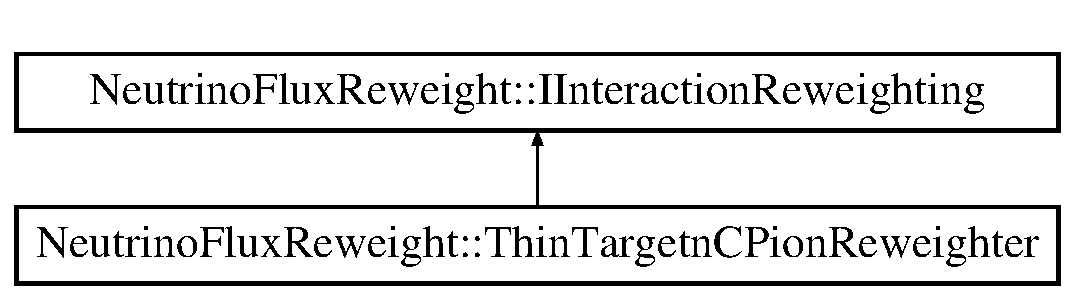
\includegraphics[height=2.000000cm]{class_neutrino_flux_reweight_1_1_thin_targetn_c_pion_reweighter}
\end{center}
\end{figure}
\subsection*{Public Member Functions}
\begin{DoxyCompactItemize}
\item 
\hyperlink{class_neutrino_flux_reweight_1_1_thin_targetn_c_pion_reweighter_a6725a74d242b394bae9df83858d8bc9e}{Thin\-Targetn\-C\-Pion\-Reweighter} (int iuniv, const \hyperlink{class_neutrino_flux_reweight_1_1_parameter_table}{Parameter\-Table} \&cv\-\_\-pars, const \hyperlink{class_neutrino_flux_reweight_1_1_parameter_table}{Parameter\-Table} \&univ\-\_\-pars)
\item 
virtual \hyperlink{class_neutrino_flux_reweight_1_1_thin_targetn_c_pion_reweighter_aacffaaca361c640139134b33fca41ec7}{$\sim$\-Thin\-Targetn\-C\-Pion\-Reweighter} ()
\item 
virtual bool \hyperlink{class_neutrino_flux_reweight_1_1_thin_targetn_c_pion_reweighter_aaeb028c4bd75fcbbae6e03aba3a7e85a}{can\-Reweight} (const \hyperlink{class_neutrino_flux_reweight_1_1_interaction_data}{Interaction\-Data} \&aa)
\begin{DoxyCompactList}\small\item\em can the particular instance of this class reweight this interaction? \end{DoxyCompactList}\item 
virtual double \hyperlink{class_neutrino_flux_reweight_1_1_thin_targetn_c_pion_reweighter_abe918e387700a09d5878cfd22dddfdd8}{calculate\-Weight} (const \hyperlink{class_neutrino_flux_reweight_1_1_interaction_data}{Interaction\-Data} \&aa)
\begin{DoxyCompactList}\small\item\em calculate a weight for this interaction given the central value parameters and the parameters for this universe. The weight is something like\-: f(cv)/f(M\-C) $\ast$ f(univ)/f(cv) where cv in this case corresponds to the best value of the parameter, given the data. If univ\-\_\-pars=cv\-\_\-pars then we are calculating a central value weight \end{DoxyCompactList}\end{DoxyCompactItemize}
\subsection*{Private Attributes}
\begin{DoxyCompactItemize}
\item 
int \hyperlink{class_neutrino_flux_reweight_1_1_thin_targetn_c_pion_reweighter_a4739c4b376e4e9d4a1b6968efddf41d8}{i\-Univ}
\item 
const \hyperlink{class_neutrino_flux_reweight_1_1_parameter_table}{Parameter\-Table} \& \hyperlink{class_neutrino_flux_reweight_1_1_thin_targetn_c_pion_reweighter_ab843f2f08ded4f483a4f80f9ee3488ed}{cv\-Pars}
\item 
const \hyperlink{class_neutrino_flux_reweight_1_1_parameter_table}{Parameter\-Table} \& \hyperlink{class_neutrino_flux_reweight_1_1_thin_targetn_c_pion_reweighter_a0ff3aa1a33a5e28c56f43ab9e6fa02b3}{univ\-Pars}
\item 
\hyperlink{class_neutrino_flux_reweight_1_1_thin_targetp_c_pion_reweighter}{Thin\-Targetp\-C\-Pion\-Reweighter} $\ast$ \hyperlink{class_neutrino_flux_reweight_1_1_thin_targetn_c_pion_reweighter_a3cd598e2a95c1cf40db298236f3551c9}{tt\-\_\-p\-C\-Pion\-Rew}
\end{DoxyCompactItemize}


\subsection{Detailed Description}
Reweighter of thin target n\-C interactions. 

Definition at line 20 of file Thin\-Targetn\-C\-Pion\-Reweighter.\-h.



\subsection{Constructor \& Destructor Documentation}
\hypertarget{class_neutrino_flux_reweight_1_1_thin_targetn_c_pion_reweighter_a6725a74d242b394bae9df83858d8bc9e}{\index{Neutrino\-Flux\-Reweight\-::\-Thin\-Targetn\-C\-Pion\-Reweighter@{Neutrino\-Flux\-Reweight\-::\-Thin\-Targetn\-C\-Pion\-Reweighter}!Thin\-Targetn\-C\-Pion\-Reweighter@{Thin\-Targetn\-C\-Pion\-Reweighter}}
\index{Thin\-Targetn\-C\-Pion\-Reweighter@{Thin\-Targetn\-C\-Pion\-Reweighter}!NeutrinoFluxReweight::ThinTargetnCPionReweighter@{Neutrino\-Flux\-Reweight\-::\-Thin\-Targetn\-C\-Pion\-Reweighter}}
\subsubsection[{Thin\-Targetn\-C\-Pion\-Reweighter}]{\setlength{\rightskip}{0pt plus 5cm}Neutrino\-Flux\-Reweight\-::\-Thin\-Targetn\-C\-Pion\-Reweighter\-::\-Thin\-Targetn\-C\-Pion\-Reweighter (
\begin{DoxyParamCaption}
\item[{int}]{iuniv, }
\item[{const {\bf Parameter\-Table} \&}]{cv\-\_\-pars, }
\item[{const {\bf Parameter\-Table} \&}]{univ\-\_\-pars}
\end{DoxyParamCaption}
)}}\label{class_neutrino_flux_reweight_1_1_thin_targetn_c_pion_reweighter_a6725a74d242b394bae9df83858d8bc9e}


Definition at line 8 of file Thin\-Targetn\-C\-Pion\-Reweighter.\-cpp.


\begin{DoxyCode}
8                                                                                                            
                            :\hyperlink{class_neutrino_flux_reweight_1_1_thin_targetn_c_pion_reweighter_a4739c4b376e4e9d4a1b6968efddf41d8}{iUniv}(iuniv),\hyperlink{class_neutrino_flux_reweight_1_1_thin_targetn_c_pion_reweighter_ab843f2f08ded4f483a4f80f9ee3488ed}{cvPars}(cv\_pars),\hyperlink{class_neutrino_flux_reweight_1_1_thin_targetn_c_pion_reweighter_a0ff3aa1a33a5e28c56f43ab9e6fa02b3}{univPars}(univ\_pars)\{
9     
10   \}
\end{DoxyCode}
\hypertarget{class_neutrino_flux_reweight_1_1_thin_targetn_c_pion_reweighter_aacffaaca361c640139134b33fca41ec7}{\index{Neutrino\-Flux\-Reweight\-::\-Thin\-Targetn\-C\-Pion\-Reweighter@{Neutrino\-Flux\-Reweight\-::\-Thin\-Targetn\-C\-Pion\-Reweighter}!$\sim$\-Thin\-Targetn\-C\-Pion\-Reweighter@{$\sim$\-Thin\-Targetn\-C\-Pion\-Reweighter}}
\index{$\sim$\-Thin\-Targetn\-C\-Pion\-Reweighter@{$\sim$\-Thin\-Targetn\-C\-Pion\-Reweighter}!NeutrinoFluxReweight::ThinTargetnCPionReweighter@{Neutrino\-Flux\-Reweight\-::\-Thin\-Targetn\-C\-Pion\-Reweighter}}
\subsubsection[{$\sim$\-Thin\-Targetn\-C\-Pion\-Reweighter}]{\setlength{\rightskip}{0pt plus 5cm}Neutrino\-Flux\-Reweight\-::\-Thin\-Targetn\-C\-Pion\-Reweighter\-::$\sim$\-Thin\-Targetn\-C\-Pion\-Reweighter (
\begin{DoxyParamCaption}
{}
\end{DoxyParamCaption}
)\hspace{0.3cm}{\ttfamily [virtual]}}}\label{class_neutrino_flux_reweight_1_1_thin_targetn_c_pion_reweighter_aacffaaca361c640139134b33fca41ec7}


Definition at line 12 of file Thin\-Targetn\-C\-Pion\-Reweighter.\-cpp.


\begin{DoxyCode}
12                                                           \{
13     
14   \}
\end{DoxyCode}


\subsection{Member Function Documentation}
\hypertarget{class_neutrino_flux_reweight_1_1_thin_targetn_c_pion_reweighter_abe918e387700a09d5878cfd22dddfdd8}{\index{Neutrino\-Flux\-Reweight\-::\-Thin\-Targetn\-C\-Pion\-Reweighter@{Neutrino\-Flux\-Reweight\-::\-Thin\-Targetn\-C\-Pion\-Reweighter}!calculate\-Weight@{calculate\-Weight}}
\index{calculate\-Weight@{calculate\-Weight}!NeutrinoFluxReweight::ThinTargetnCPionReweighter@{Neutrino\-Flux\-Reweight\-::\-Thin\-Targetn\-C\-Pion\-Reweighter}}
\subsubsection[{calculate\-Weight}]{\setlength{\rightskip}{0pt plus 5cm}double Neutrino\-Flux\-Reweight\-::\-Thin\-Targetn\-C\-Pion\-Reweighter\-::calculate\-Weight (
\begin{DoxyParamCaption}
\item[{const {\bf Interaction\-Data} \&}]{inter\-\_\-data}
\end{DoxyParamCaption}
)\hspace{0.3cm}{\ttfamily [virtual]}}}\label{class_neutrino_flux_reweight_1_1_thin_targetn_c_pion_reweighter_abe918e387700a09d5878cfd22dddfdd8}


calculate a weight for this interaction given the central value parameters and the parameters for this universe. The weight is something like\-: f(cv)/f(M\-C) $\ast$ f(univ)/f(cv) where cv in this case corresponds to the best value of the parameter, given the data. If univ\-\_\-pars=cv\-\_\-pars then we are calculating a central value weight 



Implements \hyperlink{class_neutrino_flux_reweight_1_1_i_interaction_reweighting_a49b0d73e778411d629205d23575703c3}{Neutrino\-Flux\-Reweight\-::\-I\-Interaction\-Reweighting}.



Definition at line 44 of file Thin\-Targetn\-C\-Pion\-Reweighter.\-cpp.


\begin{DoxyCode}
44                                                                              \{
45     
46     MakeReweight*  makerew =  \hyperlink{class_neutrino_flux_reweight_1_1_make_reweight_a42d1fa92a1e30bd80538188e0c9d8b4a}{MakeReweight::getInstance}();
47     \textcolor{keywordflow}{if}(\hyperlink{class_neutrino_flux_reweight_1_1_thin_targetn_c_pion_reweighter_a4739c4b376e4e9d4a1b6968efddf41d8}{iUniv}==-1)\hyperlink{class_neutrino_flux_reweight_1_1_thin_targetn_c_pion_reweighter_a3cd598e2a95c1cf40db298236f3551c9}{tt\_pCPionRew} = (makerew->cv\_rw)->THINTARGET\_PC\_PION\_Universe;
48     \textcolor{keywordflow}{else} \hyperlink{class_neutrino_flux_reweight_1_1_thin_targetn_c_pion_reweighter_a3cd598e2a95c1cf40db298236f3551c9}{tt\_pCPionRew} = (makerew->vec\_rws[\hyperlink{class_neutrino_flux_reweight_1_1_thin_targetn_c_pion_reweighter_a4739c4b376e4e9d4a1b6968efddf41d8}{iUniv}])->THINTARGET\_PC\_PION\_Universe;
49 
50     \textcolor{keywordtype}{double} inc\_mom[3]  = \{aa.Inc\_P4[0], aa.Inc\_P4[1], aa.Inc\_P4[2]\};
51     \textcolor{keywordtype}{double} prod\_mom[3] = \{aa.Prod\_P4[0],aa.Prod\_P4[1],aa.Prod\_P4[2]\};
52     \textcolor{keywordtype}{double} vtx\_int[3]  = \{aa.Vtx[0],aa.Vtx[1],aa.Vtx[2]\};
53     InteractionData intData(aa.gen, inc\_mom,2212,prod\_mom,-1*aa.Prod\_pdg,aa.Vol,aa.Proc,vtx\_int);
54 
55     \textcolor{keywordtype}{double} wgt = \hyperlink{class_neutrino_flux_reweight_1_1_thin_targetn_c_pion_reweighter_a3cd598e2a95c1cf40db298236f3551c9}{tt\_pCPionRew}->\hyperlink{class_neutrino_flux_reweight_1_1_thin_targetp_c_pion_reweighter_ab797bbeeedb04cda73feef891434cd5f}{calculateWeight}(intData);
56 
57     \textcolor{keywordflow}{if}(wgt<0)std::cout<<\textcolor{stringliteral}{"TTNCPI check wgt(<0) "}<<\hyperlink{class_neutrino_flux_reweight_1_1_thin_targetn_c_pion_reweighter_a4739c4b376e4e9d4a1b6968efddf41d8}{iUniv}<<\textcolor{stringliteral}{" "}<<aa.Inc\_P<<\textcolor{stringliteral}{" "}<<aa.xF<<\textcolor{stringliteral}{" "}<<aa.Pt<<\textcolor{stringliteral}{" "}<<aa
      .Prod\_pdg<<std::endl;
58     \textcolor{keywordflow}{return} wgt;
59       
60   \}
\end{DoxyCode}
\hypertarget{class_neutrino_flux_reweight_1_1_thin_targetn_c_pion_reweighter_aaeb028c4bd75fcbbae6e03aba3a7e85a}{\index{Neutrino\-Flux\-Reweight\-::\-Thin\-Targetn\-C\-Pion\-Reweighter@{Neutrino\-Flux\-Reweight\-::\-Thin\-Targetn\-C\-Pion\-Reweighter}!can\-Reweight@{can\-Reweight}}
\index{can\-Reweight@{can\-Reweight}!NeutrinoFluxReweight::ThinTargetnCPionReweighter@{Neutrino\-Flux\-Reweight\-::\-Thin\-Targetn\-C\-Pion\-Reweighter}}
\subsubsection[{can\-Reweight}]{\setlength{\rightskip}{0pt plus 5cm}bool Neutrino\-Flux\-Reweight\-::\-Thin\-Targetn\-C\-Pion\-Reweighter\-::can\-Reweight (
\begin{DoxyParamCaption}
\item[{const {\bf Interaction\-Data} \&}]{aa}
\end{DoxyParamCaption}
)\hspace{0.3cm}{\ttfamily [virtual]}}}\label{class_neutrino_flux_reweight_1_1_thin_targetn_c_pion_reweighter_aaeb028c4bd75fcbbae6e03aba3a7e85a}


can the particular instance of this class reweight this interaction? 



Implements \hyperlink{class_neutrino_flux_reweight_1_1_i_interaction_reweighting_aa3d1d3f37a93b02e447cf5eca333ac8d}{Neutrino\-Flux\-Reweight\-::\-I\-Interaction\-Reweighting}.



Definition at line 15 of file Thin\-Targetn\-C\-Pion\-Reweighter.\-cpp.


\begin{DoxyCode}
15                                                                        \{
16 
17     MakeReweight*  makerew =  \hyperlink{class_neutrino_flux_reweight_1_1_make_reweight_a42d1fa92a1e30bd80538188e0c9d8b4a}{MakeReweight::getInstance}();
18     \textcolor{keywordflow}{if}(\hyperlink{class_neutrino_flux_reweight_1_1_thin_targetn_c_pion_reweighter_a4739c4b376e4e9d4a1b6968efddf41d8}{iUniv}==-1)\hyperlink{class_neutrino_flux_reweight_1_1_thin_targetn_c_pion_reweighter_a3cd598e2a95c1cf40db298236f3551c9}{tt\_pCPionRew} = (makerew->cv\_rw)->THINTARGET\_PC\_PION\_Universe;
19     \textcolor{keywordflow}{else} \hyperlink{class_neutrino_flux_reweight_1_1_thin_targetn_c_pion_reweighter_a3cd598e2a95c1cf40db298236f3551c9}{tt\_pCPionRew} = (makerew->vec\_rws[\hyperlink{class_neutrino_flux_reweight_1_1_thin_targetn_c_pion_reweighter_a4739c4b376e4e9d4a1b6968efddf41d8}{iUniv}])->THINTARGET\_PC\_PION\_Universe;
20     
21     \textcolor{comment}{//checking:}
22     std::string mode(getenv(\textcolor{stringliteral}{"MODE"}));
23     \textcolor{keywordflow}{if}(aa.Inc\_pdg != 2112)\textcolor{keywordflow}{return} \textcolor{keyword}{false};
24     \textcolor{keywordflow}{if}(aa.Inc\_P < 12.0)\textcolor{keywordflow}{return} \textcolor{keyword}{false};
25     \textcolor{comment}{//volume check: }
26     \textcolor{keywordtype}{bool} is\_wrong\_volume = aa.Vol != \textcolor{stringliteral}{"TGT1"} && aa.Vol != \textcolor{stringliteral}{"BudalMonitor"} && aa.Vol != \textcolor{stringliteral}{"Budal\_HFVS"} && aa.Vol
       != \textcolor{stringliteral}{"Budal\_VFHS"};
27     \textcolor{keywordflow}{if}( (mode==\textcolor{stringliteral}{"REF"}) || (mode==\textcolor{stringliteral}{"OPT"}) )\{
28      \textcolor{comment}{// is\_wrong\_volume = aa.Vol != "TargetFinHorizontal" && aa.Vol != "TargetNoSplitSegment";}
29       is\_wrong\_volume = aa.Vol != \textcolor{stringliteral}{"TargetFinHorizontal"} && aa.Vol != \textcolor{stringliteral}{"TargetNoSplitSegment"} && aa.Vol!=\textcolor{stringliteral}{"
      tCoreLog"};     
30     \}
31     \textcolor{keywordflow}{if}(is\_wrong\_volume)\textcolor{keywordflow}{return} \textcolor{keyword}{false};
32     \textcolor{comment}{//}
33     \textcolor{keywordflow}{if}(aa.Prod\_pdg != 211 && aa.Prod\_pdg != -211)\textcolor{keywordflow}{return} \textcolor{keyword}{false};
34     
35     \textcolor{keywordtype}{double} inc\_mom[3]  = \{aa.Inc\_P4[0], aa.Inc\_P4[1], aa.Inc\_P4[2]\};
36     \textcolor{keywordtype}{double} prod\_mom[3] = \{aa.Prod\_P4[0],aa.Prod\_P4[1],aa.Prod\_P4[2]\};
37     \textcolor{keywordtype}{double} vtx\_int[3]  = \{aa.Vtx[0],aa.Vtx[1],aa.Vtx[2]\};
38     
39     InteractionData intData(aa.gen, inc\_mom,2212,prod\_mom,-1*aa.Prod\_pdg,aa.Vol,aa.Proc,vtx\_int);
40     \textcolor{keywordflow}{return} \hyperlink{class_neutrino_flux_reweight_1_1_thin_targetn_c_pion_reweighter_a3cd598e2a95c1cf40db298236f3551c9}{tt\_pCPionRew}->\hyperlink{class_neutrino_flux_reweight_1_1_thin_targetp_c_pion_reweighter_a09067dcacb294ca133e2660d61302e85}{canReweight}(intData);
41     
42   \}
\end{DoxyCode}


\subsection{Member Data Documentation}
\hypertarget{class_neutrino_flux_reweight_1_1_thin_targetn_c_pion_reweighter_ab843f2f08ded4f483a4f80f9ee3488ed}{\index{Neutrino\-Flux\-Reweight\-::\-Thin\-Targetn\-C\-Pion\-Reweighter@{Neutrino\-Flux\-Reweight\-::\-Thin\-Targetn\-C\-Pion\-Reweighter}!cv\-Pars@{cv\-Pars}}
\index{cv\-Pars@{cv\-Pars}!NeutrinoFluxReweight::ThinTargetnCPionReweighter@{Neutrino\-Flux\-Reweight\-::\-Thin\-Targetn\-C\-Pion\-Reweighter}}
\subsubsection[{cv\-Pars}]{\setlength{\rightskip}{0pt plus 5cm}const {\bf Parameter\-Table}\& Neutrino\-Flux\-Reweight\-::\-Thin\-Targetn\-C\-Pion\-Reweighter\-::cv\-Pars\hspace{0.3cm}{\ttfamily [private]}}}\label{class_neutrino_flux_reweight_1_1_thin_targetn_c_pion_reweighter_ab843f2f08ded4f483a4f80f9ee3488ed}


Definition at line 30 of file Thin\-Targetn\-C\-Pion\-Reweighter.\-h.

\hypertarget{class_neutrino_flux_reweight_1_1_thin_targetn_c_pion_reweighter_a4739c4b376e4e9d4a1b6968efddf41d8}{\index{Neutrino\-Flux\-Reweight\-::\-Thin\-Targetn\-C\-Pion\-Reweighter@{Neutrino\-Flux\-Reweight\-::\-Thin\-Targetn\-C\-Pion\-Reweighter}!i\-Univ@{i\-Univ}}
\index{i\-Univ@{i\-Univ}!NeutrinoFluxReweight::ThinTargetnCPionReweighter@{Neutrino\-Flux\-Reweight\-::\-Thin\-Targetn\-C\-Pion\-Reweighter}}
\subsubsection[{i\-Univ}]{\setlength{\rightskip}{0pt plus 5cm}int Neutrino\-Flux\-Reweight\-::\-Thin\-Targetn\-C\-Pion\-Reweighter\-::i\-Univ\hspace{0.3cm}{\ttfamily [private]}}}\label{class_neutrino_flux_reweight_1_1_thin_targetn_c_pion_reweighter_a4739c4b376e4e9d4a1b6968efddf41d8}


Definition at line 29 of file Thin\-Targetn\-C\-Pion\-Reweighter.\-h.

\hypertarget{class_neutrino_flux_reweight_1_1_thin_targetn_c_pion_reweighter_a3cd598e2a95c1cf40db298236f3551c9}{\index{Neutrino\-Flux\-Reweight\-::\-Thin\-Targetn\-C\-Pion\-Reweighter@{Neutrino\-Flux\-Reweight\-::\-Thin\-Targetn\-C\-Pion\-Reweighter}!tt\-\_\-p\-C\-Pion\-Rew@{tt\-\_\-p\-C\-Pion\-Rew}}
\index{tt\-\_\-p\-C\-Pion\-Rew@{tt\-\_\-p\-C\-Pion\-Rew}!NeutrinoFluxReweight::ThinTargetnCPionReweighter@{Neutrino\-Flux\-Reweight\-::\-Thin\-Targetn\-C\-Pion\-Reweighter}}
\subsubsection[{tt\-\_\-p\-C\-Pion\-Rew}]{\setlength{\rightskip}{0pt plus 5cm}{\bf Thin\-Targetp\-C\-Pion\-Reweighter}$\ast$ Neutrino\-Flux\-Reweight\-::\-Thin\-Targetn\-C\-Pion\-Reweighter\-::tt\-\_\-p\-C\-Pion\-Rew\hspace{0.3cm}{\ttfamily [private]}}}\label{class_neutrino_flux_reweight_1_1_thin_targetn_c_pion_reweighter_a3cd598e2a95c1cf40db298236f3551c9}


Definition at line 33 of file Thin\-Targetn\-C\-Pion\-Reweighter.\-h.

\hypertarget{class_neutrino_flux_reweight_1_1_thin_targetn_c_pion_reweighter_a0ff3aa1a33a5e28c56f43ab9e6fa02b3}{\index{Neutrino\-Flux\-Reweight\-::\-Thin\-Targetn\-C\-Pion\-Reweighter@{Neutrino\-Flux\-Reweight\-::\-Thin\-Targetn\-C\-Pion\-Reweighter}!univ\-Pars@{univ\-Pars}}
\index{univ\-Pars@{univ\-Pars}!NeutrinoFluxReweight::ThinTargetnCPionReweighter@{Neutrino\-Flux\-Reweight\-::\-Thin\-Targetn\-C\-Pion\-Reweighter}}
\subsubsection[{univ\-Pars}]{\setlength{\rightskip}{0pt plus 5cm}const {\bf Parameter\-Table}\& Neutrino\-Flux\-Reweight\-::\-Thin\-Targetn\-C\-Pion\-Reweighter\-::univ\-Pars\hspace{0.3cm}{\ttfamily [private]}}}\label{class_neutrino_flux_reweight_1_1_thin_targetn_c_pion_reweighter_a0ff3aa1a33a5e28c56f43ab9e6fa02b3}


Definition at line 31 of file Thin\-Targetn\-C\-Pion\-Reweighter.\-h.



The documentation for this class was generated from the following files\-:\begin{DoxyCompactItemize}
\item 
include/\hyperlink{_thin_targetn_c_pion_reweighter_8h}{Thin\-Targetn\-C\-Pion\-Reweighter.\-h}\item 
src/\hyperlink{_thin_targetn_c_pion_reweighter_8cpp}{Thin\-Targetn\-C\-Pion\-Reweighter.\-cpp}\end{DoxyCompactItemize}

\hypertarget{class_neutrino_flux_reweight_1_1_thin_targetnucleon_a_reweighter}{\section{Neutrino\-Flux\-Reweight\-:\-:Thin\-Targetnucleon\-A\-Reweighter Class Reference}
\label{class_neutrino_flux_reweight_1_1_thin_targetnucleon_a_reweighter}\index{Neutrino\-Flux\-Reweight\-::\-Thin\-Targetnucleon\-A\-Reweighter@{Neutrino\-Flux\-Reweight\-::\-Thin\-Targetnucleon\-A\-Reweighter}}
}


Reweighter of thin target nucleon\-A interactions.  




{\ttfamily \#include $<$Thin\-Targetnucleon\-A\-Reweighter.\-h$>$}

Inheritance diagram for Neutrino\-Flux\-Reweight\-:\-:Thin\-Targetnucleon\-A\-Reweighter\-:\begin{figure}[H]
\begin{center}
\leavevmode
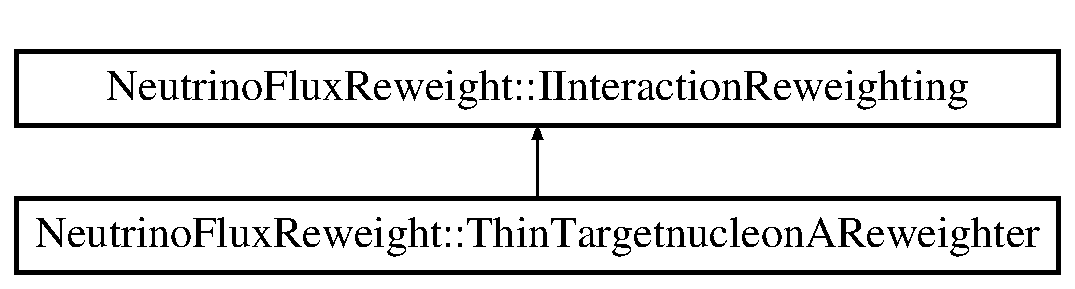
\includegraphics[height=2.000000cm]{class_neutrino_flux_reweight_1_1_thin_targetnucleon_a_reweighter}
\end{center}
\end{figure}
\subsection*{Public Member Functions}
\begin{DoxyCompactItemize}
\item 
\hyperlink{class_neutrino_flux_reweight_1_1_thin_targetnucleon_a_reweighter_a0f394f48cb0b247cf8d0137b22066832}{Thin\-Targetnucleon\-A\-Reweighter} (int iuniv, const \hyperlink{class_neutrino_flux_reweight_1_1_parameter_table}{Parameter\-Table} \&cv\-\_\-pars, const \hyperlink{class_neutrino_flux_reweight_1_1_parameter_table}{Parameter\-Table} \&univ\-\_\-pars)
\item 
virtual \hyperlink{class_neutrino_flux_reweight_1_1_thin_targetnucleon_a_reweighter_ac7a6b08a70b9cee8d5005d5e818e5065}{$\sim$\-Thin\-Targetnucleon\-A\-Reweighter} ()
\item 
virtual bool \hyperlink{class_neutrino_flux_reweight_1_1_thin_targetnucleon_a_reweighter_ac412a741a29973bbefbb3daa0cf6636a}{can\-Reweight} (const \hyperlink{class_neutrino_flux_reweight_1_1_interaction_data}{Interaction\-Data} \&aa)
\begin{DoxyCompactList}\small\item\em can the particular instance of this class reweight this interaction? \end{DoxyCompactList}\item 
virtual double \hyperlink{class_neutrino_flux_reweight_1_1_thin_targetnucleon_a_reweighter_a98d78fabb1cb7fa39372846cb57b0845}{calculate\-Weight} (const \hyperlink{class_neutrino_flux_reweight_1_1_interaction_data}{Interaction\-Data} \&aa)
\begin{DoxyCompactList}\small\item\em calculate a weight for this interaction given the central value parameters and the parameters for this universe. The weight is something like\-: f(cv)/f(M\-C) $\ast$ f(univ)/f(cv) where cv in this case corresponds to the best value of the parameter, given the data. If univ\-\_\-pars=cv\-\_\-pars then we are calculating a central value weight \end{DoxyCompactList}\end{DoxyCompactItemize}
\subsection*{Public Attributes}
\begin{DoxyCompactItemize}
\item 
std\-::vector$<$ float $>$ \hyperlink{class_neutrino_flux_reweight_1_1_thin_targetnucleon_a_reweighter_ae7012b962ce5fc1297fe56722661532a}{vbin\-\_\-data\-\_\-pip}
\item 
std\-::vector$<$ float $>$ \hyperlink{class_neutrino_flux_reweight_1_1_thin_targetnucleon_a_reweighter_ae0b6c63ce05db44c64d8b272ce3cbaed}{vbin\-\_\-data\-\_\-pim}
\item 
std\-::vector$<$ float $>$ \hyperlink{class_neutrino_flux_reweight_1_1_thin_targetnucleon_a_reweighter_acfadbda1695d49d43efe9e5a5395317b}{vbin\-\_\-data\-\_\-kap}
\item 
std\-::vector$<$ float $>$ \hyperlink{class_neutrino_flux_reweight_1_1_thin_targetnucleon_a_reweighter_ae434ebe9822621ab7e5250b4057a883d}{vbin\-\_\-data\-\_\-kam}
\item 
double \hyperlink{class_neutrino_flux_reweight_1_1_thin_targetnucleon_a_reweighter_a47e99efcf073246a61f4a5bd4db3574e}{data\-\_\-prod\-\_\-xs}
\item 
std\-::vector$<$ float $>$ \hyperlink{class_neutrino_flux_reweight_1_1_thin_targetnucleon_a_reweighter_a62d37535ba63cd757dcf40763a66d459}{vbin\-\_\-prt\-\_\-inc\-\_\-pip}
\item 
std\-::vector$<$ float $>$ \hyperlink{class_neutrino_flux_reweight_1_1_thin_targetnucleon_a_reweighter_ae1652fcc9e3b525b169b0bcb8bf22a1c}{vbin\-\_\-prt\-\_\-inc\-\_\-pim}
\item 
std\-::vector$<$ float $>$ \hyperlink{class_neutrino_flux_reweight_1_1_thin_targetnucleon_a_reweighter_a82e5925cc95dfa54adbb6b0f5af89444}{vbin\-\_\-prt\-\_\-inc\-\_\-kap}
\item 
std\-::vector$<$ float $>$ \hyperlink{class_neutrino_flux_reweight_1_1_thin_targetnucleon_a_reweighter_a846d581016c8e15e5528c64fdc5a6fee}{vbin\-\_\-prt\-\_\-inc\-\_\-kam}
\item 
std\-::vector$<$ float $>$ \hyperlink{class_neutrino_flux_reweight_1_1_thin_targetnucleon_a_reweighter_abc9e0de56770183d6108172ae1673b6d}{vbin\-\_\-prt\-\_\-inc\-\_\-k0}
\item 
std\-::vector$<$ float $>$ \hyperlink{class_neutrino_flux_reweight_1_1_thin_targetnucleon_a_reweighter_a7ac18fafe93466aae51c87b6a11eea35}{vbin\-\_\-prt\-\_\-inc\-\_\-p}
\item 
std\-::vector$<$ float $>$ \hyperlink{class_neutrino_flux_reweight_1_1_thin_targetnucleon_a_reweighter_a2f5a030bd0654de8d5d62294ca7441d9}{vbin\-\_\-prt\-\_\-inc\-\_\-n}
\item 
std\-::vector$<$ float $>$ \hyperlink{class_neutrino_flux_reweight_1_1_thin_targetnucleon_a_reweighter_ae47fb7b28a9a98bcf896bc93b96c371d}{vbin\-\_\-neu\-\_\-inc\-\_\-pip}
\item 
std\-::vector$<$ float $>$ \hyperlink{class_neutrino_flux_reweight_1_1_thin_targetnucleon_a_reweighter_a7643f9d1002efdd8030f0a2016cfd5f4}{vbin\-\_\-neu\-\_\-inc\-\_\-pim}
\item 
std\-::vector$<$ float $>$ \hyperlink{class_neutrino_flux_reweight_1_1_thin_targetnucleon_a_reweighter_a1ec58cec8bcce352e693785f7f7c7904}{vbin\-\_\-neu\-\_\-inc\-\_\-kap}
\item 
std\-::vector$<$ float $>$ \hyperlink{class_neutrino_flux_reweight_1_1_thin_targetnucleon_a_reweighter_a7c77ff20d31c4d95447e593726d267b0}{vbin\-\_\-neu\-\_\-inc\-\_\-kam}
\item 
std\-::vector$<$ float $>$ \hyperlink{class_neutrino_flux_reweight_1_1_thin_targetnucleon_a_reweighter_adaee6b1fb0e48aa2e40806ac78937b94}{vbin\-\_\-neu\-\_\-inc\-\_\-k0}
\item 
std\-::vector$<$ float $>$ \hyperlink{class_neutrino_flux_reweight_1_1_thin_targetnucleon_a_reweighter_a73c1e6b171db3486462eb3c0e6899396}{vbin\-\_\-neu\-\_\-inc\-\_\-p}
\item 
std\-::vector$<$ float $>$ \hyperlink{class_neutrino_flux_reweight_1_1_thin_targetnucleon_a_reweighter_a270e10a3f2bc7ece4a7bf35e88ca5061}{vbin\-\_\-neu\-\_\-inc\-\_\-n}
\item 
float \hyperlink{class_neutrino_flux_reweight_1_1_thin_targetnucleon_a_reweighter_a70d7724eabbb284c4a6c145d8abd9dd4}{bin\-\_\-prtleftover\-\_\-inc}
\item 
float \hyperlink{class_neutrino_flux_reweight_1_1_thin_targetnucleon_a_reweighter_a6c16f1fc945e36479f96e918392710f3}{bin\-\_\-neuleftover\-\_\-inc}
\end{DoxyCompactItemize}
\subsection*{Private Attributes}
\begin{DoxyCompactItemize}
\item 
int \hyperlink{class_neutrino_flux_reweight_1_1_thin_targetnucleon_a_reweighter_a546b2c322fe357472e17a4a901bd2212}{i\-Univ}
\item 
const \hyperlink{class_neutrino_flux_reweight_1_1_parameter_table}{Parameter\-Table} \& \hyperlink{class_neutrino_flux_reweight_1_1_thin_targetnucleon_a_reweighter_aa2690e0e126d75bbcb68ec28c8c4811a}{cv\-Pars}
\item 
const \hyperlink{class_neutrino_flux_reweight_1_1_parameter_table}{Parameter\-Table} \& \hyperlink{class_neutrino_flux_reweight_1_1_thin_targetnucleon_a_reweighter_a56d10ce15819c77e9d4a6538f403b71e}{univ\-Pars}
\item 
\hyperlink{class_neutrino_flux_reweight_1_1_thin_targetp_c_pion_reweighter}{Thin\-Targetp\-C\-Pion\-Reweighter} $\ast$ \hyperlink{class_neutrino_flux_reweight_1_1_thin_targetnucleon_a_reweighter_a0a172e21c2229793a1cc8c02bd91a10c}{tt\-\_\-p\-C\-Pion\-Rew}
\item 
\hyperlink{class_neutrino_flux_reweight_1_1_thin_targetn_c_pion_reweighter}{Thin\-Targetn\-C\-Pion\-Reweighter} $\ast$ \hyperlink{class_neutrino_flux_reweight_1_1_thin_targetnucleon_a_reweighter_ae21cb01b4e98a9d57dc4f4f61a331b1c}{tt\-\_\-n\-C\-Pion\-Rew}
\item 
\hyperlink{class_neutrino_flux_reweight_1_1_thin_targetp_c_kaon_reweighter}{Thin\-Targetp\-C\-Kaon\-Reweighter} $\ast$ \hyperlink{class_neutrino_flux_reweight_1_1_thin_targetnucleon_a_reweighter_afd58d88fc30de67bd41956efb17bd303}{tt\-\_\-p\-C\-Kaon\-Rew}
\end{DoxyCompactItemize}


\subsection{Detailed Description}
Reweighter of thin target nucleon\-A interactions. 

Definition at line 22 of file Thin\-Targetnucleon\-A\-Reweighter.\-h.



\subsection{Constructor \& Destructor Documentation}
\hypertarget{class_neutrino_flux_reweight_1_1_thin_targetnucleon_a_reweighter_a0f394f48cb0b247cf8d0137b22066832}{\index{Neutrino\-Flux\-Reweight\-::\-Thin\-Targetnucleon\-A\-Reweighter@{Neutrino\-Flux\-Reweight\-::\-Thin\-Targetnucleon\-A\-Reweighter}!Thin\-Targetnucleon\-A\-Reweighter@{Thin\-Targetnucleon\-A\-Reweighter}}
\index{Thin\-Targetnucleon\-A\-Reweighter@{Thin\-Targetnucleon\-A\-Reweighter}!NeutrinoFluxReweight::ThinTargetnucleonAReweighter@{Neutrino\-Flux\-Reweight\-::\-Thin\-Targetnucleon\-A\-Reweighter}}
\subsubsection[{Thin\-Targetnucleon\-A\-Reweighter}]{\setlength{\rightskip}{0pt plus 5cm}Neutrino\-Flux\-Reweight\-::\-Thin\-Targetnucleon\-A\-Reweighter\-::\-Thin\-Targetnucleon\-A\-Reweighter (
\begin{DoxyParamCaption}
\item[{int}]{iuniv, }
\item[{const {\bf Parameter\-Table} \&}]{cv\-\_\-pars, }
\item[{const {\bf Parameter\-Table} \&}]{univ\-\_\-pars}
\end{DoxyParamCaption}
)}}\label{class_neutrino_flux_reweight_1_1_thin_targetnucleon_a_reweighter_a0f394f48cb0b247cf8d0137b22066832}


Definition at line 10 of file Thin\-Targetnucleon\-A\-Reweighter.\-cpp.


\begin{DoxyCode}
10                                                                                                            
                                :\hyperlink{class_neutrino_flux_reweight_1_1_thin_targetnucleon_a_reweighter_a546b2c322fe357472e17a4a901bd2212}{iUniv}(iuniv),\hyperlink{class_neutrino_flux_reweight_1_1_thin_targetnucleon_a_reweighter_aa2690e0e126d75bbcb68ec28c8c4811a}{cvPars}(cv\_pars),\hyperlink{class_neutrino_flux_reweight_1_1_thin_targetnucleon_a_reweighter_a56d10ce15819c77e9d4a6538f403b71e}{univPars}(univ\_pars)\{
11     
12     ThinTargetBins* Thinbins =  \hyperlink{class_neutrino_flux_reweight_1_1_thin_target_bins_aeff5cf7220dd08322f5abac2cbc7ff33}{ThinTargetBins::getInstance}();
13     
14     \hyperlink{class_neutrino_flux_reweight_1_1_thin_targetnucleon_a_reweighter_ae7012b962ce5fc1297fe56722661532a}{vbin\_data\_pip}.reserve(Thinbins->GetNbins\_material\_scaling());
15     \hyperlink{class_neutrino_flux_reweight_1_1_thin_targetnucleon_a_reweighter_ae0b6c63ce05db44c64d8b272ce3cbaed}{vbin\_data\_pim}.reserve(Thinbins->GetNbins\_material\_scaling());
16     \hyperlink{class_neutrino_flux_reweight_1_1_thin_targetnucleon_a_reweighter_acfadbda1695d49d43efe9e5a5395317b}{vbin\_data\_kap}.reserve(Thinbins->GetNbins\_material\_scaling());
17     \hyperlink{class_neutrino_flux_reweight_1_1_thin_targetnucleon_a_reweighter_ae434ebe9822621ab7e5250b4057a883d}{vbin\_data\_kam}.reserve(Thinbins->GetNbins\_material\_scaling());
18     
19     \textcolor{comment}{//Currently, We are using the same number of xF ranges for nucleon inc. and meson inc.}
20     \hyperlink{class_neutrino_flux_reweight_1_1_thin_targetnucleon_a_reweighter_a62d37535ba63cd757dcf40763a66d459}{vbin\_prt\_inc\_pip}.reserve(Thinbins->GetNbins\_meson\_incident());
21     \hyperlink{class_neutrino_flux_reweight_1_1_thin_targetnucleon_a_reweighter_ae1652fcc9e3b525b169b0bcb8bf22a1c}{vbin\_prt\_inc\_pim}.reserve(Thinbins->GetNbins\_meson\_incident());
22     \hyperlink{class_neutrino_flux_reweight_1_1_thin_targetnucleon_a_reweighter_a82e5925cc95dfa54adbb6b0f5af89444}{vbin\_prt\_inc\_kap}.reserve(Thinbins->GetNbins\_meson\_incident());
23     \hyperlink{class_neutrino_flux_reweight_1_1_thin_targetnucleon_a_reweighter_a846d581016c8e15e5528c64fdc5a6fee}{vbin\_prt\_inc\_kam}.reserve(Thinbins->GetNbins\_meson\_incident());
24     \hyperlink{class_neutrino_flux_reweight_1_1_thin_targetnucleon_a_reweighter_abc9e0de56770183d6108172ae1673b6d}{vbin\_prt\_inc\_k0}.reserve(Thinbins->GetNbins\_meson\_incident());
25     \hyperlink{class_neutrino_flux_reweight_1_1_thin_targetnucleon_a_reweighter_a7ac18fafe93466aae51c87b6a11eea35}{vbin\_prt\_inc\_p}.reserve(Thinbins->GetNbins\_meson\_incident());
26     \hyperlink{class_neutrino_flux_reweight_1_1_thin_targetnucleon_a_reweighter_a2f5a030bd0654de8d5d62294ca7441d9}{vbin\_prt\_inc\_n}.reserve(Thinbins->GetNbins\_meson\_incident());
27     \hyperlink{class_neutrino_flux_reweight_1_1_thin_targetnucleon_a_reweighter_ae47fb7b28a9a98bcf896bc93b96c371d}{vbin\_neu\_inc\_pip}.reserve(Thinbins->GetNbins\_meson\_incident());
28     \hyperlink{class_neutrino_flux_reweight_1_1_thin_targetnucleon_a_reweighter_a7643f9d1002efdd8030f0a2016cfd5f4}{vbin\_neu\_inc\_pim}.reserve(Thinbins->GetNbins\_meson\_incident());
29     \hyperlink{class_neutrino_flux_reweight_1_1_thin_targetnucleon_a_reweighter_a1ec58cec8bcce352e693785f7f7c7904}{vbin\_neu\_inc\_kap}.reserve(Thinbins->GetNbins\_meson\_incident());
30     \hyperlink{class_neutrino_flux_reweight_1_1_thin_targetnucleon_a_reweighter_a7c77ff20d31c4d95447e593726d267b0}{vbin\_neu\_inc\_kam}.reserve(Thinbins->GetNbins\_meson\_incident());
31     \hyperlink{class_neutrino_flux_reweight_1_1_thin_targetnucleon_a_reweighter_adaee6b1fb0e48aa2e40806ac78937b94}{vbin\_neu\_inc\_k0}.reserve(Thinbins->GetNbins\_meson\_incident());
32     \hyperlink{class_neutrino_flux_reweight_1_1_thin_targetnucleon_a_reweighter_a73c1e6b171db3486462eb3c0e6899396}{vbin\_neu\_inc\_p}.reserve(Thinbins->GetNbins\_meson\_incident());
33     \hyperlink{class_neutrino_flux_reweight_1_1_thin_targetnucleon_a_reweighter_a270e10a3f2bc7ece4a7bf35e88ca5061}{vbin\_neu\_inc\_n}.reserve(Thinbins->GetNbins\_meson\_incident());
34 
35     \textcolor{comment}{// const boost::interprocess::flat\_map<std::string, double>& cv\_table   = cvPars.getMap();}
36     \textcolor{comment}{// const boost::interprocess::flat\_map<std::string, double>& univ\_table = univPars.getMap();}
37     \textcolor{keywordtype}{char} namepar[100];
38     
39     \hyperlink{class_neutrino_flux_reweight_1_1_thin_targetnucleon_a_reweighter_a47e99efcf073246a61f4a5bd4db3574e}{data\_prod\_xs} = \hyperlink{class_neutrino_flux_reweight_1_1_thin_targetnucleon_a_reweighter_a56d10ce15819c77e9d4a6538f403b71e}{univPars}.\hyperlink{class_neutrino_flux_reweight_1_1_parameter_table_acb7dc8335b65b116f6092f2fa57ca5ed}{getParameterValue}(\textcolor{stringliteral}{"prod\_prtC\_xsec"});
40     
41     \textcolor{comment}{//4 particles}
42     \textcolor{keyword}{const} \textcolor{keywordtype}{char}* cinc[4] = \{\textcolor{stringliteral}{"pip"},\textcolor{stringliteral}{"pim"},\textcolor{stringliteral}{"kap"},\textcolor{stringliteral}{"kam"}\};    
43     \textcolor{keywordflow}{for}(\textcolor{keywordtype}{int} ii=0;ii<4;ii++)\{
44       \textcolor{keywordflow}{for}(\textcolor{keywordtype}{int} jj=0;jj<Thinbins->GetNbins\_material\_scaling();jj++)\{
45         sprintf(namepar,\textcolor{stringliteral}{"ThinTarget\_material\_scaling\_%s\_%d"},cinc[ii],jj);
46         \textcolor{keywordtype}{double} dataval = \hyperlink{class_neutrino_flux_reweight_1_1_thin_targetnucleon_a_reweighter_a56d10ce15819c77e9d4a6538f403b71e}{univPars}.\hyperlink{class_neutrino_flux_reweight_1_1_parameter_table_acb7dc8335b65b116f6092f2fa57ca5ed}{getParameterValue}(std::string(namepar));
47         \textcolor{keywordflow}{if}(ii==0)\hyperlink{class_neutrino_flux_reweight_1_1_thin_targetnucleon_a_reweighter_ae7012b962ce5fc1297fe56722661532a}{vbin\_data\_pip}.push\_back(dataval);
48         \textcolor{keywordflow}{if}(ii==1)\hyperlink{class_neutrino_flux_reweight_1_1_thin_targetnucleon_a_reweighter_ae0b6c63ce05db44c64d8b272ce3cbaed}{vbin\_data\_pim}.push\_back(dataval);
49         \textcolor{keywordflow}{if}(ii==2)\hyperlink{class_neutrino_flux_reweight_1_1_thin_targetnucleon_a_reweighter_acfadbda1695d49d43efe9e5a5395317b}{vbin\_data\_kap}.push\_back(dataval);
50         \textcolor{keywordflow}{if}(ii==3)\hyperlink{class_neutrino_flux_reweight_1_1_thin_targetnucleon_a_reweighter_ae434ebe9822621ab7e5250b4057a883d}{vbin\_data\_kam}.push\_back(dataval);
51       \}
52     \}
53 
54     \textcolor{comment}{//for all nucleons incident not covered by any thin target reweighters    }
55     \textcolor{comment}{//2 incident nucleons, 7 produced particles:}
56     \textcolor{keyword}{const} \textcolor{keywordtype}{char}* nuinc[2] = \{\textcolor{stringliteral}{"prt"},\textcolor{stringliteral}{"neu"}\};
57     \textcolor{keyword}{const} \textcolor{keywordtype}{char}* cpro[7] = \{\textcolor{stringliteral}{"pip"},\textcolor{stringliteral}{"pim"},\textcolor{stringliteral}{"kap"},\textcolor{stringliteral}{"kam"},\textcolor{stringliteral}{"k0"},\textcolor{stringliteral}{"n"},\textcolor{stringliteral}{"p"}\};
58     
59     \textcolor{keywordflow}{for}(\textcolor{keywordtype}{int} ii=0;ii<2;ii++)\{
60       \textcolor{keywordflow}{for}(\textcolor{keywordtype}{int} jj=0;jj<7;jj++)\{
61         \textcolor{keywordflow}{for}(\textcolor{keywordtype}{int} kk=0;kk<Thinbins->GetNbins\_meson\_incident();kk++)\{
62           sprintf(namepar,\textcolor{stringliteral}{"ThinTarget\_%s\_incident\_%s\_%d"},nuinc[ii],cpro[jj],kk);
63           \textcolor{keywordtype}{double} dataval = \hyperlink{class_neutrino_flux_reweight_1_1_thin_targetnucleon_a_reweighter_a56d10ce15819c77e9d4a6538f403b71e}{univPars}.\hyperlink{class_neutrino_flux_reweight_1_1_parameter_table_acb7dc8335b65b116f6092f2fa57ca5ed}{getParameterValue}(std::string(namepar));
64           \textcolor{keywordflow}{if}(ii==0 && jj==0)\hyperlink{class_neutrino_flux_reweight_1_1_thin_targetnucleon_a_reweighter_a62d37535ba63cd757dcf40763a66d459}{vbin\_prt\_inc\_pip}.push\_back(dataval);
65           \textcolor{keywordflow}{if}(ii==0 && jj==1)\hyperlink{class_neutrino_flux_reweight_1_1_thin_targetnucleon_a_reweighter_ae1652fcc9e3b525b169b0bcb8bf22a1c}{vbin\_prt\_inc\_pim}.push\_back(dataval);
66           \textcolor{keywordflow}{if}(ii==0 && jj==2)\hyperlink{class_neutrino_flux_reweight_1_1_thin_targetnucleon_a_reweighter_a82e5925cc95dfa54adbb6b0f5af89444}{vbin\_prt\_inc\_kap}.push\_back(dataval);
67           \textcolor{keywordflow}{if}(ii==0 && jj==3)\hyperlink{class_neutrino_flux_reweight_1_1_thin_targetnucleon_a_reweighter_a846d581016c8e15e5528c64fdc5a6fee}{vbin\_prt\_inc\_kam}.push\_back(dataval);
68           \textcolor{keywordflow}{if}(ii==0 && jj==4)\hyperlink{class_neutrino_flux_reweight_1_1_thin_targetnucleon_a_reweighter_abc9e0de56770183d6108172ae1673b6d}{vbin\_prt\_inc\_k0}.push\_back(dataval);
69           \textcolor{keywordflow}{if}(ii==0 && jj==5)\hyperlink{class_neutrino_flux_reweight_1_1_thin_targetnucleon_a_reweighter_a2f5a030bd0654de8d5d62294ca7441d9}{vbin\_prt\_inc\_n}.push\_back(dataval);
70           \textcolor{keywordflow}{if}(ii==0 && jj==6)\hyperlink{class_neutrino_flux_reweight_1_1_thin_targetnucleon_a_reweighter_a7ac18fafe93466aae51c87b6a11eea35}{vbin\_prt\_inc\_p}.push\_back(dataval);
71           \textcolor{keywordflow}{if}(ii==1 && jj==0)\hyperlink{class_neutrino_flux_reweight_1_1_thin_targetnucleon_a_reweighter_ae47fb7b28a9a98bcf896bc93b96c371d}{vbin\_neu\_inc\_pip}.push\_back(dataval);
72           \textcolor{keywordflow}{if}(ii==1 && jj==1)\hyperlink{class_neutrino_flux_reweight_1_1_thin_targetnucleon_a_reweighter_a7643f9d1002efdd8030f0a2016cfd5f4}{vbin\_neu\_inc\_pim}.push\_back(dataval);
73           \textcolor{keywordflow}{if}(ii==1 && jj==2)\hyperlink{class_neutrino_flux_reweight_1_1_thin_targetnucleon_a_reweighter_a1ec58cec8bcce352e693785f7f7c7904}{vbin\_neu\_inc\_kap}.push\_back(dataval);
74           \textcolor{keywordflow}{if}(ii==1 && jj==3)\hyperlink{class_neutrino_flux_reweight_1_1_thin_targetnucleon_a_reweighter_a7c77ff20d31c4d95447e593726d267b0}{vbin\_neu\_inc\_kam}.push\_back(dataval);
75           \textcolor{keywordflow}{if}(ii==1 && jj==4)\hyperlink{class_neutrino_flux_reweight_1_1_thin_targetnucleon_a_reweighter_adaee6b1fb0e48aa2e40806ac78937b94}{vbin\_neu\_inc\_k0}.push\_back(dataval);
76           \textcolor{keywordflow}{if}(ii==1 && jj==5)\hyperlink{class_neutrino_flux_reweight_1_1_thin_targetnucleon_a_reweighter_a270e10a3f2bc7ece4a7bf35e88ca5061}{vbin\_neu\_inc\_n}.push\_back(dataval);
77           \textcolor{keywordflow}{if}(ii==1 && jj==6)\hyperlink{class_neutrino_flux_reweight_1_1_thin_targetnucleon_a_reweighter_a73c1e6b171db3486462eb3c0e6899396}{vbin\_neu\_inc\_p}.push\_back(dataval);
78         \}
79       \}
80     \}     
81     \textcolor{comment}{//left over:}
82     sprintf(namepar,\textcolor{stringliteral}{"ThinTarget\_prtleftover\_incident\_%d"},0);
83     \hyperlink{class_neutrino_flux_reweight_1_1_thin_targetnucleon_a_reweighter_a70d7724eabbb284c4a6c145d8abd9dd4}{bin\_prtleftover\_inc} = \hyperlink{class_neutrino_flux_reweight_1_1_thin_targetnucleon_a_reweighter_a56d10ce15819c77e9d4a6538f403b71e}{univPars}.\hyperlink{class_neutrino_flux_reweight_1_1_parameter_table_acb7dc8335b65b116f6092f2fa57ca5ed}{getParameterValue}(
      std::string(namepar));
84     sprintf(namepar,\textcolor{stringliteral}{"ThinTarget\_neuleftover\_incident\_%d"},0);
85     \hyperlink{class_neutrino_flux_reweight_1_1_thin_targetnucleon_a_reweighter_a6c16f1fc945e36479f96e918392710f3}{bin\_neuleftover\_inc} = \hyperlink{class_neutrino_flux_reweight_1_1_thin_targetnucleon_a_reweighter_a56d10ce15819c77e9d4a6538f403b71e}{univPars}.\hyperlink{class_neutrino_flux_reweight_1_1_parameter_table_acb7dc8335b65b116f6092f2fa57ca5ed}{getParameterValue}(
      std::string(namepar));
86     
87   \}
\end{DoxyCode}
\hypertarget{class_neutrino_flux_reweight_1_1_thin_targetnucleon_a_reweighter_ac7a6b08a70b9cee8d5005d5e818e5065}{\index{Neutrino\-Flux\-Reweight\-::\-Thin\-Targetnucleon\-A\-Reweighter@{Neutrino\-Flux\-Reweight\-::\-Thin\-Targetnucleon\-A\-Reweighter}!$\sim$\-Thin\-Targetnucleon\-A\-Reweighter@{$\sim$\-Thin\-Targetnucleon\-A\-Reweighter}}
\index{$\sim$\-Thin\-Targetnucleon\-A\-Reweighter@{$\sim$\-Thin\-Targetnucleon\-A\-Reweighter}!NeutrinoFluxReweight::ThinTargetnucleonAReweighter@{Neutrino\-Flux\-Reweight\-::\-Thin\-Targetnucleon\-A\-Reweighter}}
\subsubsection[{$\sim$\-Thin\-Targetnucleon\-A\-Reweighter}]{\setlength{\rightskip}{0pt plus 5cm}Neutrino\-Flux\-Reweight\-::\-Thin\-Targetnucleon\-A\-Reweighter\-::$\sim$\-Thin\-Targetnucleon\-A\-Reweighter (
\begin{DoxyParamCaption}
{}
\end{DoxyParamCaption}
)\hspace{0.3cm}{\ttfamily [virtual]}}}\label{class_neutrino_flux_reweight_1_1_thin_targetnucleon_a_reweighter_ac7a6b08a70b9cee8d5005d5e818e5065}


Definition at line 89 of file Thin\-Targetnucleon\-A\-Reweighter.\-cpp.


\begin{DoxyCode}
89                                                              \{
90     
91   \}
\end{DoxyCode}


\subsection{Member Function Documentation}
\hypertarget{class_neutrino_flux_reweight_1_1_thin_targetnucleon_a_reweighter_a98d78fabb1cb7fa39372846cb57b0845}{\index{Neutrino\-Flux\-Reweight\-::\-Thin\-Targetnucleon\-A\-Reweighter@{Neutrino\-Flux\-Reweight\-::\-Thin\-Targetnucleon\-A\-Reweighter}!calculate\-Weight@{calculate\-Weight}}
\index{calculate\-Weight@{calculate\-Weight}!NeutrinoFluxReweight::ThinTargetnucleonAReweighter@{Neutrino\-Flux\-Reweight\-::\-Thin\-Targetnucleon\-A\-Reweighter}}
\subsubsection[{calculate\-Weight}]{\setlength{\rightskip}{0pt plus 5cm}double Neutrino\-Flux\-Reweight\-::\-Thin\-Targetnucleon\-A\-Reweighter\-::calculate\-Weight (
\begin{DoxyParamCaption}
\item[{const {\bf Interaction\-Data} \&}]{inter\-\_\-data}
\end{DoxyParamCaption}
)\hspace{0.3cm}{\ttfamily [virtual]}}}\label{class_neutrino_flux_reweight_1_1_thin_targetnucleon_a_reweighter_a98d78fabb1cb7fa39372846cb57b0845}


calculate a weight for this interaction given the central value parameters and the parameters for this universe. The weight is something like\-: f(cv)/f(M\-C) $\ast$ f(univ)/f(cv) where cv in this case corresponds to the best value of the parameter, given the data. If univ\-\_\-pars=cv\-\_\-pars then we are calculating a central value weight 



Implements \hyperlink{class_neutrino_flux_reweight_1_1_i_interaction_reweighting_a49b0d73e778411d629205d23575703c3}{Neutrino\-Flux\-Reweight\-::\-I\-Interaction\-Reweighting}.



Definition at line 130 of file Thin\-Targetnucleon\-A\-Reweighter.\-cpp.


\begin{DoxyCode}
130                                                                                \{
131 
132     \textcolor{keywordtype}{double} wgt = 1.0;
133     std::string mode(getenv(\textcolor{stringliteral}{"MODE"}));
134     \textcolor{comment}{//checking:}
135     \textcolor{keywordflow}{if}(aa.Inc\_pdg != 2212 && aa.Inc\_pdg != 2112)\textcolor{keywordflow}{return} wgt;
136     \textcolor{comment}{/*}
137 \textcolor{comment}{      if(aa.Inc\_P < 12.0)return wgt;}
138 \textcolor{comment}{      if(aa.Vol == "TGT1" || aa.Vol == "BudalMonitor")return wgt;}
139 \textcolor{comment}{      if(aa.Prod\_pdg != 211 && aa.Prod\_pdg != -211 && aa.Prod\_pdg !=321 && aa.Prod\_pdg != -321 &&
       aa.Prod\_pdg !=310 && aa.Prod\_pdg != 130)return wgt;}
140 \textcolor{comment}{    */}
141     ThinTargetBins*  Thinbins =  \hyperlink{class_neutrino_flux_reweight_1_1_thin_target_bins_aeff5cf7220dd08322f5abac2cbc7ff33}{ThinTargetBins::getInstance}();
142     \textcolor{keywordtype}{int} bin = Thinbins->material\_scaling\_BinID(aa.xF,aa.Pt,aa.Prod\_pdg);
143     \textcolor{keywordtype}{bool} is\_data\_based = (aa.Inc\_P >= 12.0) && (aa.Vol != \textcolor{stringliteral}{"TGT1"} && aa.Vol != \textcolor{stringliteral}{"BudalMonitor"} && aa.Vol != \textcolor{stringliteral}{"
      Budal\_HFVS"} && aa.Vol != \textcolor{stringliteral}{"Budal\_VFHS"}) && 
144       (aa.Prod\_pdg == 211 || aa.Prod\_pdg == -211 || aa.Prod\_pdg ==321 || aa.Prod\_pdg == -321 || aa.Prod\_pdg
       ==310 || aa.Prod\_pdg == 130) &&
145       (bin>=0);
146     
147     \textcolor{keywordflow}{if}((mode==\textcolor{stringliteral}{"REF"})||(mode==\textcolor{stringliteral}{"OPT"}))\{
148       is\_data\_based = (aa.Inc\_P >= 12.0) && (aa.Vol != \textcolor{stringliteral}{"TargetNoSplitSegment"} && aa.Vol != \textcolor{stringliteral}{"
      TargetFinHorizontal"}) && aa.Vol!= \textcolor{stringliteral}{"tCoreLog"} && 
149         (aa.Prod\_pdg == 211 || aa.Prod\_pdg == -211 || aa.Prod\_pdg ==321 || aa.Prod\_pdg == -321 || aa.
      Prod\_pdg ==310 || aa.Prod\_pdg == 130) &&
150         (bin>=0);
151     \}
152     \textcolor{keywordtype}{double} inc\_mom[3]  = \{aa.Inc\_P4[0], aa.Inc\_P4[1], aa.Inc\_P4[2]\};
153     \textcolor{keywordtype}{double} prod\_mom[3] = \{aa.Prod\_P4[0],aa.Prod\_P4[1],aa.Prod\_P4[2]\};
154     \textcolor{keywordtype}{double} vtx\_int[3]  = \{aa.Vtx[0],aa.Vtx[1],aa.Vtx[2]\};
155     std::string tgtent = \textcolor{stringliteral}{"TGT1"};
156     \textcolor{keywordflow}{if}((mode==\textcolor{stringliteral}{"REF"})||(mode==\textcolor{stringliteral}{"OPT"}))tgtent= \textcolor{stringliteral}{"tCoreLog"};\textcolor{comment}{//"TargetFinHorizontal";}
157     InteractionData aux\_aa2(aa.gen,inc\_mom,aa.Inc\_pdg,prod\_mom,aa.Prod\_pdg,tgtent,aa.Proc,vtx\_int);
158     
159     \textcolor{keywordtype}{bool} not\_handled = \textcolor{keyword}{false};
160     \textcolor{keywordflow}{if}(is\_data\_based)\{
161       
162       ThinTargetMC*  mc =  \hyperlink{class_neutrino_flux_reweight_1_1_thin_target_m_c_a2a114747fed2677cd3b7213555c002b9}{ThinTargetMC::getInstance}(); 
163       \textcolor{keywordtype}{double} mc\_prod   = mc->getMCxs\_pC\_piK(0,aa.Inc\_P);
164       \textcolor{keywordtype}{double} fact\_gen0 = \hyperlink{class_neutrino_flux_reweight_1_1_thin_targetnucleon_a_reweighter_a47e99efcf073246a61f4a5bd4db3574e}{data\_prod\_xs}/mc\_prod;
165       MakeReweight*  makerew =  \hyperlink{class_neutrino_flux_reweight_1_1_make_reweight_a42d1fa92a1e30bd80538188e0c9d8b4a}{MakeReweight::getInstance}();
166 
167       \textcolor{keywordflow}{if}(aa.Inc\_pdg == 2212)\{
168 
169         \textcolor{keywordflow}{if}(aa.Prod\_pdg == 211 || aa.Prod\_pdg == -211)\{
170 
171           \textcolor{keywordflow}{if}(\hyperlink{class_neutrino_flux_reweight_1_1_thin_targetnucleon_a_reweighter_a546b2c322fe357472e17a4a901bd2212}{iUniv}==-1)\hyperlink{class_neutrino_flux_reweight_1_1_thin_targetnucleon_a_reweighter_a0a172e21c2229793a1cc8c02bd91a10c}{tt\_pCPionRew} = (makerew->cv\_rw)->THINTARGET\_PC\_PION\_Universe;
172           \textcolor{keywordflow}{else} \hyperlink{class_neutrino_flux_reweight_1_1_thin_targetnucleon_a_reweighter_a0a172e21c2229793a1cc8c02bd91a10c}{tt\_pCPionRew} = (makerew->vec\_rws[\hyperlink{class_neutrino_flux_reweight_1_1_thin_targetnucleon_a_reweighter_a546b2c322fe357472e17a4a901bd2212}{iUniv}])->THINTARGET\_PC\_PION\_Universe;    
173           
174           \textcolor{keywordflow}{if}(\hyperlink{class_neutrino_flux_reweight_1_1_thin_targetnucleon_a_reweighter_a0a172e21c2229793a1cc8c02bd91a10c}{tt\_pCPionRew}->\hyperlink{class_neutrino_flux_reweight_1_1_thin_targetp_c_pion_reweighter_a09067dcacb294ca133e2660d61302e85}{canReweight}(aux\_aa2))\{
175             wgt = \hyperlink{class_neutrino_flux_reweight_1_1_thin_targetnucleon_a_reweighter_a0a172e21c2229793a1cc8c02bd91a10c}{tt\_pCPionRew}->\hyperlink{class_neutrino_flux_reweight_1_1_thin_targetp_c_pion_reweighter_ab797bbeeedb04cda73feef891434cd5f}{calculateWeight}(aux\_aa2);
176             \textcolor{keywordflow}{if}(aux\_aa2.gen == 0) wgt *= fact\_gen0;
177           \}
178           \textcolor{keywordflow}{else} not\_handled = \textcolor{keyword}{true};
179         \}      
180 
181         \textcolor{keywordflow}{else} \textcolor{keywordflow}{if}(aa.Prod\_pdg == 321 || aa.Prod\_pdg == -321 || aa.Prod\_pdg == 130 || aa.Prod\_pdg == 310)\{
182 
183           \textcolor{keywordflow}{if}(\hyperlink{class_neutrino_flux_reweight_1_1_thin_targetnucleon_a_reweighter_a546b2c322fe357472e17a4a901bd2212}{iUniv}==-1)\hyperlink{class_neutrino_flux_reweight_1_1_thin_targetnucleon_a_reweighter_afd58d88fc30de67bd41956efb17bd303}{tt\_pCKaonRew} = (makerew->cv\_rw)->THINTARGET\_PC\_KAON\_Universe;
184           \textcolor{keywordflow}{else} \hyperlink{class_neutrino_flux_reweight_1_1_thin_targetnucleon_a_reweighter_afd58d88fc30de67bd41956efb17bd303}{tt\_pCKaonRew} = (makerew->vec\_rws[\hyperlink{class_neutrino_flux_reweight_1_1_thin_targetnucleon_a_reweighter_a546b2c322fe357472e17a4a901bd2212}{iUniv}])->THINTARGET\_PC\_KAON\_Universe;    
185           
186           \textcolor{keywordflow}{if}(\hyperlink{class_neutrino_flux_reweight_1_1_thin_targetnucleon_a_reweighter_afd58d88fc30de67bd41956efb17bd303}{tt\_pCKaonRew}->\hyperlink{class_neutrino_flux_reweight_1_1_thin_targetp_c_kaon_reweighter_a78d9307c378b36d660feb54ba8114a9a}{canReweight}(aux\_aa2))\{
187             wgt = \hyperlink{class_neutrino_flux_reweight_1_1_thin_targetnucleon_a_reweighter_afd58d88fc30de67bd41956efb17bd303}{tt\_pCKaonRew}->\hyperlink{class_neutrino_flux_reweight_1_1_thin_targetp_c_kaon_reweighter_a64f5f6df3b44240b56b863206773ca9a}{calculateWeight}(aux\_aa2);
188             \textcolor{keywordflow}{if}(aux\_aa2.gen == 0) wgt *= fact\_gen0;
189           \}
190           \textcolor{keywordflow}{else} not\_handled = \textcolor{keyword}{true};
191         \}
192         \textcolor{keywordflow}{else} not\_handled = \textcolor{keyword}{true};
193       \}
194       \textcolor{keywordflow}{else} \textcolor{keywordflow}{if}(aa.Inc\_pdg == 2112)\{
195         \textcolor{keywordflow}{if}(aa.Prod\_pdg == 211 || aa.Prod\_pdg == -211)\{
196 
197           \textcolor{keywordflow}{if}(\hyperlink{class_neutrino_flux_reweight_1_1_thin_targetnucleon_a_reweighter_a546b2c322fe357472e17a4a901bd2212}{iUniv}==-1)\hyperlink{class_neutrino_flux_reweight_1_1_thin_targetnucleon_a_reweighter_ae21cb01b4e98a9d57dc4f4f61a331b1c}{tt\_nCPionRew} = (makerew->cv\_rw)->THINTARGET\_NC\_PION\_Universe;
198           \textcolor{keywordflow}{else} \hyperlink{class_neutrino_flux_reweight_1_1_thin_targetnucleon_a_reweighter_ae21cb01b4e98a9d57dc4f4f61a331b1c}{tt\_nCPionRew} = (makerew->vec\_rws[\hyperlink{class_neutrino_flux_reweight_1_1_thin_targetnucleon_a_reweighter_a546b2c322fe357472e17a4a901bd2212}{iUniv}])->THINTARGET\_NC\_PION\_Universe;    
199 
200           \textcolor{keywordflow}{if}(\hyperlink{class_neutrino_flux_reweight_1_1_thin_targetnucleon_a_reweighter_ae21cb01b4e98a9d57dc4f4f61a331b1c}{tt\_nCPionRew}->\hyperlink{class_neutrino_flux_reweight_1_1_thin_targetn_c_pion_reweighter_aaeb028c4bd75fcbbae6e03aba3a7e85a}{canReweight}(aux\_aa2))\{
201             wgt = \hyperlink{class_neutrino_flux_reweight_1_1_thin_targetnucleon_a_reweighter_ae21cb01b4e98a9d57dc4f4f61a331b1c}{tt\_nCPionRew}->\hyperlink{class_neutrino_flux_reweight_1_1_thin_targetn_c_pion_reweighter_abe918e387700a09d5878cfd22dddfdd8}{calculateWeight}(aux\_aa2);
202             \textcolor{keywordflow}{if}(aux\_aa2.gen == 0) wgt *= fact\_gen0;
203           \}      
204           \textcolor{keywordflow}{else} not\_handled = \textcolor{keyword}{true};
205         \}
206         \textcolor{keywordflow}{else} not\_handled = \textcolor{keyword}{true};
207       \}
208       \textcolor{keywordflow}{else} not\_handled = \textcolor{keyword}{true};
209       
210       \textcolor{keywordtype}{double} scaling = 1.0;
211       \textcolor{keywordflow}{if}(aa.Prod\_pdg == 211)scaling = \hyperlink{class_neutrino_flux_reweight_1_1_thin_targetnucleon_a_reweighter_ae7012b962ce5fc1297fe56722661532a}{vbin\_data\_pip}[bin];
212       \textcolor{keywordflow}{if}(aa.Prod\_pdg ==-211)scaling = \hyperlink{class_neutrino_flux_reweight_1_1_thin_targetnucleon_a_reweighter_ae0b6c63ce05db44c64d8b272ce3cbaed}{vbin\_data\_pim}[bin];
213       \textcolor{keywordflow}{if}(aa.Prod\_pdg == 321)scaling = \hyperlink{class_neutrino_flux_reweight_1_1_thin_targetnucleon_a_reweighter_acfadbda1695d49d43efe9e5a5395317b}{vbin\_data\_kap}[bin];
214       \textcolor{keywordflow}{if}(aa.Prod\_pdg ==-321)scaling = \hyperlink{class_neutrino_flux_reweight_1_1_thin_targetnucleon_a_reweighter_ae434ebe9822621ab7e5250b4057a883d}{vbin\_data\_kam}[bin];
215       \textcolor{keywordflow}{if}(aa.Prod\_pdg == 310 || aa.Prod\_pdg == 130)scaling = \hyperlink{class_neutrino_flux_reweight_1_1_thin_targetnucleon_a_reweighter_acfadbda1695d49d43efe9e5a5395317b}{vbin\_data\_kap}[bin];    
216       wgt *= scaling;
217       \textcolor{keywordflow}{if}(!not\_handled)\textcolor{keywordflow}{return} wgt;
218     \} 
219  
220     \textcolor{comment}{//trick... using a function for meson incident... same binning.}
221     \textcolor{keywordtype}{int} binnu      = Thinbins->meson\_inc\_BinID(aa.xF,aa.Pt,211);
222     \textcolor{keywordflow}{if}(binnu<0)\textcolor{keywordflow}{return} 1.0;
223 
224     \textcolor{keywordflow}{if}(aa.Inc\_pdg ==2212)\{
225       \textcolor{keywordflow}{if}(aa.Prod\_pdg == 211) wgt = \hyperlink{class_neutrino_flux_reweight_1_1_thin_targetnucleon_a_reweighter_a62d37535ba63cd757dcf40763a66d459}{vbin\_prt\_inc\_pip}[binnu];
226       \textcolor{keywordflow}{else} \textcolor{keywordflow}{if}(aa.Prod\_pdg ==-211) wgt = \hyperlink{class_neutrino_flux_reweight_1_1_thin_targetnucleon_a_reweighter_ae1652fcc9e3b525b169b0bcb8bf22a1c}{vbin\_prt\_inc\_pim}[binnu];
227       \textcolor{keywordflow}{else} \textcolor{keywordflow}{if}(aa.Prod\_pdg == 321) wgt = \hyperlink{class_neutrino_flux_reweight_1_1_thin_targetnucleon_a_reweighter_a82e5925cc95dfa54adbb6b0f5af89444}{vbin\_prt\_inc\_kap}[binnu];
228       \textcolor{keywordflow}{else} \textcolor{keywordflow}{if}(aa.Prod\_pdg ==-321) wgt = \hyperlink{class_neutrino_flux_reweight_1_1_thin_targetnucleon_a_reweighter_a846d581016c8e15e5528c64fdc5a6fee}{vbin\_prt\_inc\_kam}[binnu];
229       \textcolor{keywordflow}{else} \textcolor{keywordflow}{if}(aa.Prod\_pdg ==130 || aa.Prod\_pdg ==310) wgt = \hyperlink{class_neutrino_flux_reweight_1_1_thin_targetnucleon_a_reweighter_abc9e0de56770183d6108172ae1673b6d}{vbin\_prt\_inc\_k0}[binnu];
230       \textcolor{keywordflow}{else} \textcolor{keywordflow}{if}(aa.Prod\_pdg ==2212) wgt = \hyperlink{class_neutrino_flux_reweight_1_1_thin_targetnucleon_a_reweighter_a7ac18fafe93466aae51c87b6a11eea35}{vbin\_prt\_inc\_p}[binnu];
231       \textcolor{keywordflow}{else} \textcolor{keywordflow}{if}(aa.Prod\_pdg ==2112) wgt = \hyperlink{class_neutrino_flux_reweight_1_1_thin_targetnucleon_a_reweighter_a2f5a030bd0654de8d5d62294ca7441d9}{vbin\_prt\_inc\_n}[binnu];    
232       \textcolor{keywordflow}{else} wgt = \hyperlink{class_neutrino_flux_reweight_1_1_thin_targetnucleon_a_reweighter_a70d7724eabbb284c4a6c145d8abd9dd4}{bin\_prtleftover\_inc};        
233     \}
234     \textcolor{keywordflow}{else} \textcolor{keywordflow}{if}(aa.Inc\_pdg ==2112)\{
235       \textcolor{keywordflow}{if}(aa.Prod\_pdg == 211) wgt = \hyperlink{class_neutrino_flux_reweight_1_1_thin_targetnucleon_a_reweighter_ae47fb7b28a9a98bcf896bc93b96c371d}{vbin\_neu\_inc\_pip}[binnu];
236       \textcolor{keywordflow}{else} \textcolor{keywordflow}{if}(aa.Prod\_pdg ==-211) wgt = \hyperlink{class_neutrino_flux_reweight_1_1_thin_targetnucleon_a_reweighter_a7643f9d1002efdd8030f0a2016cfd5f4}{vbin\_neu\_inc\_pim}[binnu];
237       \textcolor{keywordflow}{else} \textcolor{keywordflow}{if}(aa.Prod\_pdg == 321) wgt = \hyperlink{class_neutrino_flux_reweight_1_1_thin_targetnucleon_a_reweighter_a1ec58cec8bcce352e693785f7f7c7904}{vbin\_neu\_inc\_kap}[binnu];
238       \textcolor{keywordflow}{else} \textcolor{keywordflow}{if}(aa.Prod\_pdg ==-321) wgt = \hyperlink{class_neutrino_flux_reweight_1_1_thin_targetnucleon_a_reweighter_a7c77ff20d31c4d95447e593726d267b0}{vbin\_neu\_inc\_kam}[binnu];
239       \textcolor{keywordflow}{else} \textcolor{keywordflow}{if}(aa.Prod\_pdg ==130 || aa.Prod\_pdg ==310) wgt = \hyperlink{class_neutrino_flux_reweight_1_1_thin_targetnucleon_a_reweighter_adaee6b1fb0e48aa2e40806ac78937b94}{vbin\_neu\_inc\_k0}[binnu];
240       \textcolor{keywordflow}{else} \textcolor{keywordflow}{if}(aa.Prod\_pdg ==2212) wgt = \hyperlink{class_neutrino_flux_reweight_1_1_thin_targetnucleon_a_reweighter_a73c1e6b171db3486462eb3c0e6899396}{vbin\_neu\_inc\_p}[binnu];
241       \textcolor{keywordflow}{else} \textcolor{keywordflow}{if}(aa.Prod\_pdg ==2112) wgt = \hyperlink{class_neutrino_flux_reweight_1_1_thin_targetnucleon_a_reweighter_a270e10a3f2bc7ece4a7bf35e88ca5061}{vbin\_neu\_inc\_n}[binnu];
242       \textcolor{keywordflow}{else} wgt = \hyperlink{class_neutrino_flux_reweight_1_1_thin_targetnucleon_a_reweighter_a6c16f1fc945e36479f96e918392710f3}{bin\_neuleftover\_inc};        
243     \}                                           
244   
245     \textcolor{keywordflow}{return} wgt;
246     
247   \}
\end{DoxyCode}
\hypertarget{class_neutrino_flux_reweight_1_1_thin_targetnucleon_a_reweighter_ac412a741a29973bbefbb3daa0cf6636a}{\index{Neutrino\-Flux\-Reweight\-::\-Thin\-Targetnucleon\-A\-Reweighter@{Neutrino\-Flux\-Reweight\-::\-Thin\-Targetnucleon\-A\-Reweighter}!can\-Reweight@{can\-Reweight}}
\index{can\-Reweight@{can\-Reweight}!NeutrinoFluxReweight::ThinTargetnucleonAReweighter@{Neutrino\-Flux\-Reweight\-::\-Thin\-Targetnucleon\-A\-Reweighter}}
\subsubsection[{can\-Reweight}]{\setlength{\rightskip}{0pt plus 5cm}bool Neutrino\-Flux\-Reweight\-::\-Thin\-Targetnucleon\-A\-Reweighter\-::can\-Reweight (
\begin{DoxyParamCaption}
\item[{const {\bf Interaction\-Data} \&}]{aa}
\end{DoxyParamCaption}
)\hspace{0.3cm}{\ttfamily [virtual]}}}\label{class_neutrino_flux_reweight_1_1_thin_targetnucleon_a_reweighter_ac412a741a29973bbefbb3daa0cf6636a}


can the particular instance of this class reweight this interaction? 



Implements \hyperlink{class_neutrino_flux_reweight_1_1_i_interaction_reweighting_aa3d1d3f37a93b02e447cf5eca333ac8d}{Neutrino\-Flux\-Reweight\-::\-I\-Interaction\-Reweighting}.



Definition at line 92 of file Thin\-Targetnucleon\-A\-Reweighter.\-cpp.


\begin{DoxyCode}
92                                                                          \{
93 
94     \textcolor{comment}{//checking:}
95     \textcolor{keywordflow}{if}(aa.Inc\_pdg != 2212 && aa.Inc\_pdg != 2112)\textcolor{keywordflow}{return} \textcolor{keyword}{false};
96     \textcolor{comment}{//  if(aa.Inc\_P < 12.0)return false;}
97     \textcolor{comment}{// if(aa.Vol == "TGT1" || aa.Vol == "BudalMonitor")return false;}
98     \textcolor{comment}{//if(aa.Prod\_pdg != 211 && aa.Prod\_pdg != -211 && aa.Prod\_pdg !=321 && aa.Prod\_pdg != -321 &&
       aa.Prod\_pdg !=310 && aa.Prod\_pdg != 130)return false;}
99     
100     \textcolor{comment}{// ThinTargetBins*  Thinbins =  ThinTargetBins::getInstance();}
101     \textcolor{comment}{//int bin = Thinbins->material\_scaling\_BinID(aa.xF,aa.Pt,aa.Prod\_pdg);}
102     \textcolor{comment}{// if(bin<0)return false;}
103     
104     \textcolor{comment}{/*}
105 \textcolor{comment}{      MakeReweight*  makerew =  MakeReweight::getInstance();}
106 \textcolor{comment}{      if(aa.Inc\_pdg == 2212)\{}
107 \textcolor{comment}{      if(aa.Prod\_pdg == 211 || aa.Prod\_pdg == -211)\{}
108 \textcolor{comment}{      if(iUniv==-1)tt\_pCPionRew = (makerew->cv\_rw)->THINTARGET\_PC\_PION\_Universe;}
109 \textcolor{comment}{      else tt\_pCPionRew = (makerew->vec\_rws[iUniv])->THINTARGET\_PC\_PION\_Universe; }
110 \textcolor{comment}{      return tt\_pCPionRew->canReweight(*aux\_aa);}
111 \textcolor{comment}{      \}}
112 \textcolor{comment}{      else if(aa.Prod\_pdg == 321 || aa.Prod\_pdg == -321 || aa.Prod\_pdg == 310 || aa.Prod\_pdg == 130)\{}
113 \textcolor{comment}{      if(iUniv==-1)tt\_pCKaonRew = (makerew->cv\_rw)->THINTARGET\_PC\_KAON\_Universe;}
114 \textcolor{comment}{      else tt\_pCKaonRew = (makerew->vec\_rws[iUniv])->THINTARGET\_PC\_KAON\_Universe;  }
115 \textcolor{comment}{      return tt\_pCKaonRew->canReweight(*aux\_aa);}
116 \textcolor{comment}{      \}}
117 \textcolor{comment}{      \}}
118 \textcolor{comment}{      else if(aa.Inc\_pdg == 2112)\{}
119 \textcolor{comment}{      if(aa.Prod\_pdg == 211 || aa.Prod\_pdg == -211)\{}
120 \textcolor{comment}{      if(iUniv==-1)tt\_nCPionRew = (makerew->cv\_rw)->THINTARGET\_NC\_PION\_Universe;}
121 \textcolor{comment}{      else tt\_nCPionRew = (makerew->vec\_rws[iUniv])->THINTARGET\_NC\_PION\_Universe;}
122 \textcolor{comment}{      return tt\_nCPionRew->canReweight(*aux\_aa);}
123 \textcolor{comment}{      \}      }
124 \textcolor{comment}{      \}}
125 \textcolor{comment}{    */}
126 
127     \textcolor{keywordflow}{return} \textcolor{keyword}{true};
128   \}
\end{DoxyCode}


\subsection{Member Data Documentation}
\hypertarget{class_neutrino_flux_reweight_1_1_thin_targetnucleon_a_reweighter_a6c16f1fc945e36479f96e918392710f3}{\index{Neutrino\-Flux\-Reweight\-::\-Thin\-Targetnucleon\-A\-Reweighter@{Neutrino\-Flux\-Reweight\-::\-Thin\-Targetnucleon\-A\-Reweighter}!bin\-\_\-neuleftover\-\_\-inc@{bin\-\_\-neuleftover\-\_\-inc}}
\index{bin\-\_\-neuleftover\-\_\-inc@{bin\-\_\-neuleftover\-\_\-inc}!NeutrinoFluxReweight::ThinTargetnucleonAReweighter@{Neutrino\-Flux\-Reweight\-::\-Thin\-Targetnucleon\-A\-Reweighter}}
\subsubsection[{bin\-\_\-neuleftover\-\_\-inc}]{\setlength{\rightskip}{0pt plus 5cm}float Neutrino\-Flux\-Reweight\-::\-Thin\-Targetnucleon\-A\-Reweighter\-::bin\-\_\-neuleftover\-\_\-inc}}\label{class_neutrino_flux_reweight_1_1_thin_targetnucleon_a_reweighter_a6c16f1fc945e36479f96e918392710f3}


Definition at line 32 of file Thin\-Targetnucleon\-A\-Reweighter.\-h.

\hypertarget{class_neutrino_flux_reweight_1_1_thin_targetnucleon_a_reweighter_a70d7724eabbb284c4a6c145d8abd9dd4}{\index{Neutrino\-Flux\-Reweight\-::\-Thin\-Targetnucleon\-A\-Reweighter@{Neutrino\-Flux\-Reweight\-::\-Thin\-Targetnucleon\-A\-Reweighter}!bin\-\_\-prtleftover\-\_\-inc@{bin\-\_\-prtleftover\-\_\-inc}}
\index{bin\-\_\-prtleftover\-\_\-inc@{bin\-\_\-prtleftover\-\_\-inc}!NeutrinoFluxReweight::ThinTargetnucleonAReweighter@{Neutrino\-Flux\-Reweight\-::\-Thin\-Targetnucleon\-A\-Reweighter}}
\subsubsection[{bin\-\_\-prtleftover\-\_\-inc}]{\setlength{\rightskip}{0pt plus 5cm}float Neutrino\-Flux\-Reweight\-::\-Thin\-Targetnucleon\-A\-Reweighter\-::bin\-\_\-prtleftover\-\_\-inc}}\label{class_neutrino_flux_reweight_1_1_thin_targetnucleon_a_reweighter_a70d7724eabbb284c4a6c145d8abd9dd4}


Definition at line 32 of file Thin\-Targetnucleon\-A\-Reweighter.\-h.

\hypertarget{class_neutrino_flux_reweight_1_1_thin_targetnucleon_a_reweighter_aa2690e0e126d75bbcb68ec28c8c4811a}{\index{Neutrino\-Flux\-Reweight\-::\-Thin\-Targetnucleon\-A\-Reweighter@{Neutrino\-Flux\-Reweight\-::\-Thin\-Targetnucleon\-A\-Reweighter}!cv\-Pars@{cv\-Pars}}
\index{cv\-Pars@{cv\-Pars}!NeutrinoFluxReweight::ThinTargetnucleonAReweighter@{Neutrino\-Flux\-Reweight\-::\-Thin\-Targetnucleon\-A\-Reweighter}}
\subsubsection[{cv\-Pars}]{\setlength{\rightskip}{0pt plus 5cm}const {\bf Parameter\-Table}\& Neutrino\-Flux\-Reweight\-::\-Thin\-Targetnucleon\-A\-Reweighter\-::cv\-Pars\hspace{0.3cm}{\ttfamily [private]}}}\label{class_neutrino_flux_reweight_1_1_thin_targetnucleon_a_reweighter_aa2690e0e126d75bbcb68ec28c8c4811a}


Definition at line 35 of file Thin\-Targetnucleon\-A\-Reweighter.\-h.

\hypertarget{class_neutrino_flux_reweight_1_1_thin_targetnucleon_a_reweighter_a47e99efcf073246a61f4a5bd4db3574e}{\index{Neutrino\-Flux\-Reweight\-::\-Thin\-Targetnucleon\-A\-Reweighter@{Neutrino\-Flux\-Reweight\-::\-Thin\-Targetnucleon\-A\-Reweighter}!data\-\_\-prod\-\_\-xs@{data\-\_\-prod\-\_\-xs}}
\index{data\-\_\-prod\-\_\-xs@{data\-\_\-prod\-\_\-xs}!NeutrinoFluxReweight::ThinTargetnucleonAReweighter@{Neutrino\-Flux\-Reweight\-::\-Thin\-Targetnucleon\-A\-Reweighter}}
\subsubsection[{data\-\_\-prod\-\_\-xs}]{\setlength{\rightskip}{0pt plus 5cm}double Neutrino\-Flux\-Reweight\-::\-Thin\-Targetnucleon\-A\-Reweighter\-::data\-\_\-prod\-\_\-xs}}\label{class_neutrino_flux_reweight_1_1_thin_targetnucleon_a_reweighter_a47e99efcf073246a61f4a5bd4db3574e}


Definition at line 29 of file Thin\-Targetnucleon\-A\-Reweighter.\-h.

\hypertarget{class_neutrino_flux_reweight_1_1_thin_targetnucleon_a_reweighter_a546b2c322fe357472e17a4a901bd2212}{\index{Neutrino\-Flux\-Reweight\-::\-Thin\-Targetnucleon\-A\-Reweighter@{Neutrino\-Flux\-Reweight\-::\-Thin\-Targetnucleon\-A\-Reweighter}!i\-Univ@{i\-Univ}}
\index{i\-Univ@{i\-Univ}!NeutrinoFluxReweight::ThinTargetnucleonAReweighter@{Neutrino\-Flux\-Reweight\-::\-Thin\-Targetnucleon\-A\-Reweighter}}
\subsubsection[{i\-Univ}]{\setlength{\rightskip}{0pt plus 5cm}int Neutrino\-Flux\-Reweight\-::\-Thin\-Targetnucleon\-A\-Reweighter\-::i\-Univ\hspace{0.3cm}{\ttfamily [private]}}}\label{class_neutrino_flux_reweight_1_1_thin_targetnucleon_a_reweighter_a546b2c322fe357472e17a4a901bd2212}


Definition at line 34 of file Thin\-Targetnucleon\-A\-Reweighter.\-h.

\hypertarget{class_neutrino_flux_reweight_1_1_thin_targetnucleon_a_reweighter_ae21cb01b4e98a9d57dc4f4f61a331b1c}{\index{Neutrino\-Flux\-Reweight\-::\-Thin\-Targetnucleon\-A\-Reweighter@{Neutrino\-Flux\-Reweight\-::\-Thin\-Targetnucleon\-A\-Reweighter}!tt\-\_\-n\-C\-Pion\-Rew@{tt\-\_\-n\-C\-Pion\-Rew}}
\index{tt\-\_\-n\-C\-Pion\-Rew@{tt\-\_\-n\-C\-Pion\-Rew}!NeutrinoFluxReweight::ThinTargetnucleonAReweighter@{Neutrino\-Flux\-Reweight\-::\-Thin\-Targetnucleon\-A\-Reweighter}}
\subsubsection[{tt\-\_\-n\-C\-Pion\-Rew}]{\setlength{\rightskip}{0pt plus 5cm}{\bf Thin\-Targetn\-C\-Pion\-Reweighter}$\ast$ Neutrino\-Flux\-Reweight\-::\-Thin\-Targetnucleon\-A\-Reweighter\-::tt\-\_\-n\-C\-Pion\-Rew\hspace{0.3cm}{\ttfamily [private]}}}\label{class_neutrino_flux_reweight_1_1_thin_targetnucleon_a_reweighter_ae21cb01b4e98a9d57dc4f4f61a331b1c}


Definition at line 39 of file Thin\-Targetnucleon\-A\-Reweighter.\-h.

\hypertarget{class_neutrino_flux_reweight_1_1_thin_targetnucleon_a_reweighter_afd58d88fc30de67bd41956efb17bd303}{\index{Neutrino\-Flux\-Reweight\-::\-Thin\-Targetnucleon\-A\-Reweighter@{Neutrino\-Flux\-Reweight\-::\-Thin\-Targetnucleon\-A\-Reweighter}!tt\-\_\-p\-C\-Kaon\-Rew@{tt\-\_\-p\-C\-Kaon\-Rew}}
\index{tt\-\_\-p\-C\-Kaon\-Rew@{tt\-\_\-p\-C\-Kaon\-Rew}!NeutrinoFluxReweight::ThinTargetnucleonAReweighter@{Neutrino\-Flux\-Reweight\-::\-Thin\-Targetnucleon\-A\-Reweighter}}
\subsubsection[{tt\-\_\-p\-C\-Kaon\-Rew}]{\setlength{\rightskip}{0pt plus 5cm}{\bf Thin\-Targetp\-C\-Kaon\-Reweighter}$\ast$ Neutrino\-Flux\-Reweight\-::\-Thin\-Targetnucleon\-A\-Reweighter\-::tt\-\_\-p\-C\-Kaon\-Rew\hspace{0.3cm}{\ttfamily [private]}}}\label{class_neutrino_flux_reweight_1_1_thin_targetnucleon_a_reweighter_afd58d88fc30de67bd41956efb17bd303}


Definition at line 40 of file Thin\-Targetnucleon\-A\-Reweighter.\-h.

\hypertarget{class_neutrino_flux_reweight_1_1_thin_targetnucleon_a_reweighter_a0a172e21c2229793a1cc8c02bd91a10c}{\index{Neutrino\-Flux\-Reweight\-::\-Thin\-Targetnucleon\-A\-Reweighter@{Neutrino\-Flux\-Reweight\-::\-Thin\-Targetnucleon\-A\-Reweighter}!tt\-\_\-p\-C\-Pion\-Rew@{tt\-\_\-p\-C\-Pion\-Rew}}
\index{tt\-\_\-p\-C\-Pion\-Rew@{tt\-\_\-p\-C\-Pion\-Rew}!NeutrinoFluxReweight::ThinTargetnucleonAReweighter@{Neutrino\-Flux\-Reweight\-::\-Thin\-Targetnucleon\-A\-Reweighter}}
\subsubsection[{tt\-\_\-p\-C\-Pion\-Rew}]{\setlength{\rightskip}{0pt plus 5cm}{\bf Thin\-Targetp\-C\-Pion\-Reweighter}$\ast$ Neutrino\-Flux\-Reweight\-::\-Thin\-Targetnucleon\-A\-Reweighter\-::tt\-\_\-p\-C\-Pion\-Rew\hspace{0.3cm}{\ttfamily [private]}}}\label{class_neutrino_flux_reweight_1_1_thin_targetnucleon_a_reweighter_a0a172e21c2229793a1cc8c02bd91a10c}


Definition at line 38 of file Thin\-Targetnucleon\-A\-Reweighter.\-h.

\hypertarget{class_neutrino_flux_reweight_1_1_thin_targetnucleon_a_reweighter_a56d10ce15819c77e9d4a6538f403b71e}{\index{Neutrino\-Flux\-Reweight\-::\-Thin\-Targetnucleon\-A\-Reweighter@{Neutrino\-Flux\-Reweight\-::\-Thin\-Targetnucleon\-A\-Reweighter}!univ\-Pars@{univ\-Pars}}
\index{univ\-Pars@{univ\-Pars}!NeutrinoFluxReweight::ThinTargetnucleonAReweighter@{Neutrino\-Flux\-Reweight\-::\-Thin\-Targetnucleon\-A\-Reweighter}}
\subsubsection[{univ\-Pars}]{\setlength{\rightskip}{0pt plus 5cm}const {\bf Parameter\-Table}\& Neutrino\-Flux\-Reweight\-::\-Thin\-Targetnucleon\-A\-Reweighter\-::univ\-Pars\hspace{0.3cm}{\ttfamily [private]}}}\label{class_neutrino_flux_reweight_1_1_thin_targetnucleon_a_reweighter_a56d10ce15819c77e9d4a6538f403b71e}


Definition at line 36 of file Thin\-Targetnucleon\-A\-Reweighter.\-h.

\hypertarget{class_neutrino_flux_reweight_1_1_thin_targetnucleon_a_reweighter_ae434ebe9822621ab7e5250b4057a883d}{\index{Neutrino\-Flux\-Reweight\-::\-Thin\-Targetnucleon\-A\-Reweighter@{Neutrino\-Flux\-Reweight\-::\-Thin\-Targetnucleon\-A\-Reweighter}!vbin\-\_\-data\-\_\-kam@{vbin\-\_\-data\-\_\-kam}}
\index{vbin\-\_\-data\-\_\-kam@{vbin\-\_\-data\-\_\-kam}!NeutrinoFluxReweight::ThinTargetnucleonAReweighter@{Neutrino\-Flux\-Reweight\-::\-Thin\-Targetnucleon\-A\-Reweighter}}
\subsubsection[{vbin\-\_\-data\-\_\-kam}]{\setlength{\rightskip}{0pt plus 5cm}std\-::vector$<$float$>$ Neutrino\-Flux\-Reweight\-::\-Thin\-Targetnucleon\-A\-Reweighter\-::vbin\-\_\-data\-\_\-kam}}\label{class_neutrino_flux_reweight_1_1_thin_targetnucleon_a_reweighter_ae434ebe9822621ab7e5250b4057a883d}


Definition at line 28 of file Thin\-Targetnucleon\-A\-Reweighter.\-h.

\hypertarget{class_neutrino_flux_reweight_1_1_thin_targetnucleon_a_reweighter_acfadbda1695d49d43efe9e5a5395317b}{\index{Neutrino\-Flux\-Reweight\-::\-Thin\-Targetnucleon\-A\-Reweighter@{Neutrino\-Flux\-Reweight\-::\-Thin\-Targetnucleon\-A\-Reweighter}!vbin\-\_\-data\-\_\-kap@{vbin\-\_\-data\-\_\-kap}}
\index{vbin\-\_\-data\-\_\-kap@{vbin\-\_\-data\-\_\-kap}!NeutrinoFluxReweight::ThinTargetnucleonAReweighter@{Neutrino\-Flux\-Reweight\-::\-Thin\-Targetnucleon\-A\-Reweighter}}
\subsubsection[{vbin\-\_\-data\-\_\-kap}]{\setlength{\rightskip}{0pt plus 5cm}std\-::vector$<$float$>$ Neutrino\-Flux\-Reweight\-::\-Thin\-Targetnucleon\-A\-Reweighter\-::vbin\-\_\-data\-\_\-kap}}\label{class_neutrino_flux_reweight_1_1_thin_targetnucleon_a_reweighter_acfadbda1695d49d43efe9e5a5395317b}


Definition at line 28 of file Thin\-Targetnucleon\-A\-Reweighter.\-h.

\hypertarget{class_neutrino_flux_reweight_1_1_thin_targetnucleon_a_reweighter_ae0b6c63ce05db44c64d8b272ce3cbaed}{\index{Neutrino\-Flux\-Reweight\-::\-Thin\-Targetnucleon\-A\-Reweighter@{Neutrino\-Flux\-Reweight\-::\-Thin\-Targetnucleon\-A\-Reweighter}!vbin\-\_\-data\-\_\-pim@{vbin\-\_\-data\-\_\-pim}}
\index{vbin\-\_\-data\-\_\-pim@{vbin\-\_\-data\-\_\-pim}!NeutrinoFluxReweight::ThinTargetnucleonAReweighter@{Neutrino\-Flux\-Reweight\-::\-Thin\-Targetnucleon\-A\-Reweighter}}
\subsubsection[{vbin\-\_\-data\-\_\-pim}]{\setlength{\rightskip}{0pt plus 5cm}std\-::vector$<$float$>$ Neutrino\-Flux\-Reweight\-::\-Thin\-Targetnucleon\-A\-Reweighter\-::vbin\-\_\-data\-\_\-pim}}\label{class_neutrino_flux_reweight_1_1_thin_targetnucleon_a_reweighter_ae0b6c63ce05db44c64d8b272ce3cbaed}


Definition at line 28 of file Thin\-Targetnucleon\-A\-Reweighter.\-h.

\hypertarget{class_neutrino_flux_reweight_1_1_thin_targetnucleon_a_reweighter_ae7012b962ce5fc1297fe56722661532a}{\index{Neutrino\-Flux\-Reweight\-::\-Thin\-Targetnucleon\-A\-Reweighter@{Neutrino\-Flux\-Reweight\-::\-Thin\-Targetnucleon\-A\-Reweighter}!vbin\-\_\-data\-\_\-pip@{vbin\-\_\-data\-\_\-pip}}
\index{vbin\-\_\-data\-\_\-pip@{vbin\-\_\-data\-\_\-pip}!NeutrinoFluxReweight::ThinTargetnucleonAReweighter@{Neutrino\-Flux\-Reweight\-::\-Thin\-Targetnucleon\-A\-Reweighter}}
\subsubsection[{vbin\-\_\-data\-\_\-pip}]{\setlength{\rightskip}{0pt plus 5cm}std\-::vector$<$float$>$ Neutrino\-Flux\-Reweight\-::\-Thin\-Targetnucleon\-A\-Reweighter\-::vbin\-\_\-data\-\_\-pip}}\label{class_neutrino_flux_reweight_1_1_thin_targetnucleon_a_reweighter_ae7012b962ce5fc1297fe56722661532a}


Definition at line 28 of file Thin\-Targetnucleon\-A\-Reweighter.\-h.

\hypertarget{class_neutrino_flux_reweight_1_1_thin_targetnucleon_a_reweighter_adaee6b1fb0e48aa2e40806ac78937b94}{\index{Neutrino\-Flux\-Reweight\-::\-Thin\-Targetnucleon\-A\-Reweighter@{Neutrino\-Flux\-Reweight\-::\-Thin\-Targetnucleon\-A\-Reweighter}!vbin\-\_\-neu\-\_\-inc\-\_\-k0@{vbin\-\_\-neu\-\_\-inc\-\_\-k0}}
\index{vbin\-\_\-neu\-\_\-inc\-\_\-k0@{vbin\-\_\-neu\-\_\-inc\-\_\-k0}!NeutrinoFluxReweight::ThinTargetnucleonAReweighter@{Neutrino\-Flux\-Reweight\-::\-Thin\-Targetnucleon\-A\-Reweighter}}
\subsubsection[{vbin\-\_\-neu\-\_\-inc\-\_\-k0}]{\setlength{\rightskip}{0pt plus 5cm}std\-::vector$<$float$>$ Neutrino\-Flux\-Reweight\-::\-Thin\-Targetnucleon\-A\-Reweighter\-::vbin\-\_\-neu\-\_\-inc\-\_\-k0}}\label{class_neutrino_flux_reweight_1_1_thin_targetnucleon_a_reweighter_adaee6b1fb0e48aa2e40806ac78937b94}


Definition at line 31 of file Thin\-Targetnucleon\-A\-Reweighter.\-h.

\hypertarget{class_neutrino_flux_reweight_1_1_thin_targetnucleon_a_reweighter_a7c77ff20d31c4d95447e593726d267b0}{\index{Neutrino\-Flux\-Reweight\-::\-Thin\-Targetnucleon\-A\-Reweighter@{Neutrino\-Flux\-Reweight\-::\-Thin\-Targetnucleon\-A\-Reweighter}!vbin\-\_\-neu\-\_\-inc\-\_\-kam@{vbin\-\_\-neu\-\_\-inc\-\_\-kam}}
\index{vbin\-\_\-neu\-\_\-inc\-\_\-kam@{vbin\-\_\-neu\-\_\-inc\-\_\-kam}!NeutrinoFluxReweight::ThinTargetnucleonAReweighter@{Neutrino\-Flux\-Reweight\-::\-Thin\-Targetnucleon\-A\-Reweighter}}
\subsubsection[{vbin\-\_\-neu\-\_\-inc\-\_\-kam}]{\setlength{\rightskip}{0pt plus 5cm}std\-::vector$<$float$>$ Neutrino\-Flux\-Reweight\-::\-Thin\-Targetnucleon\-A\-Reweighter\-::vbin\-\_\-neu\-\_\-inc\-\_\-kam}}\label{class_neutrino_flux_reweight_1_1_thin_targetnucleon_a_reweighter_a7c77ff20d31c4d95447e593726d267b0}


Definition at line 31 of file Thin\-Targetnucleon\-A\-Reweighter.\-h.

\hypertarget{class_neutrino_flux_reweight_1_1_thin_targetnucleon_a_reweighter_a1ec58cec8bcce352e693785f7f7c7904}{\index{Neutrino\-Flux\-Reweight\-::\-Thin\-Targetnucleon\-A\-Reweighter@{Neutrino\-Flux\-Reweight\-::\-Thin\-Targetnucleon\-A\-Reweighter}!vbin\-\_\-neu\-\_\-inc\-\_\-kap@{vbin\-\_\-neu\-\_\-inc\-\_\-kap}}
\index{vbin\-\_\-neu\-\_\-inc\-\_\-kap@{vbin\-\_\-neu\-\_\-inc\-\_\-kap}!NeutrinoFluxReweight::ThinTargetnucleonAReweighter@{Neutrino\-Flux\-Reweight\-::\-Thin\-Targetnucleon\-A\-Reweighter}}
\subsubsection[{vbin\-\_\-neu\-\_\-inc\-\_\-kap}]{\setlength{\rightskip}{0pt plus 5cm}std\-::vector$<$float$>$ Neutrino\-Flux\-Reweight\-::\-Thin\-Targetnucleon\-A\-Reweighter\-::vbin\-\_\-neu\-\_\-inc\-\_\-kap}}\label{class_neutrino_flux_reweight_1_1_thin_targetnucleon_a_reweighter_a1ec58cec8bcce352e693785f7f7c7904}


Definition at line 31 of file Thin\-Targetnucleon\-A\-Reweighter.\-h.

\hypertarget{class_neutrino_flux_reweight_1_1_thin_targetnucleon_a_reweighter_a270e10a3f2bc7ece4a7bf35e88ca5061}{\index{Neutrino\-Flux\-Reweight\-::\-Thin\-Targetnucleon\-A\-Reweighter@{Neutrino\-Flux\-Reweight\-::\-Thin\-Targetnucleon\-A\-Reweighter}!vbin\-\_\-neu\-\_\-inc\-\_\-n@{vbin\-\_\-neu\-\_\-inc\-\_\-n}}
\index{vbin\-\_\-neu\-\_\-inc\-\_\-n@{vbin\-\_\-neu\-\_\-inc\-\_\-n}!NeutrinoFluxReweight::ThinTargetnucleonAReweighter@{Neutrino\-Flux\-Reweight\-::\-Thin\-Targetnucleon\-A\-Reweighter}}
\subsubsection[{vbin\-\_\-neu\-\_\-inc\-\_\-n}]{\setlength{\rightskip}{0pt plus 5cm}std\-::vector$<$float$>$ Neutrino\-Flux\-Reweight\-::\-Thin\-Targetnucleon\-A\-Reweighter\-::vbin\-\_\-neu\-\_\-inc\-\_\-n}}\label{class_neutrino_flux_reweight_1_1_thin_targetnucleon_a_reweighter_a270e10a3f2bc7ece4a7bf35e88ca5061}


Definition at line 31 of file Thin\-Targetnucleon\-A\-Reweighter.\-h.

\hypertarget{class_neutrino_flux_reweight_1_1_thin_targetnucleon_a_reweighter_a73c1e6b171db3486462eb3c0e6899396}{\index{Neutrino\-Flux\-Reweight\-::\-Thin\-Targetnucleon\-A\-Reweighter@{Neutrino\-Flux\-Reweight\-::\-Thin\-Targetnucleon\-A\-Reweighter}!vbin\-\_\-neu\-\_\-inc\-\_\-p@{vbin\-\_\-neu\-\_\-inc\-\_\-p}}
\index{vbin\-\_\-neu\-\_\-inc\-\_\-p@{vbin\-\_\-neu\-\_\-inc\-\_\-p}!NeutrinoFluxReweight::ThinTargetnucleonAReweighter@{Neutrino\-Flux\-Reweight\-::\-Thin\-Targetnucleon\-A\-Reweighter}}
\subsubsection[{vbin\-\_\-neu\-\_\-inc\-\_\-p}]{\setlength{\rightskip}{0pt plus 5cm}std\-::vector$<$float$>$ Neutrino\-Flux\-Reweight\-::\-Thin\-Targetnucleon\-A\-Reweighter\-::vbin\-\_\-neu\-\_\-inc\-\_\-p}}\label{class_neutrino_flux_reweight_1_1_thin_targetnucleon_a_reweighter_a73c1e6b171db3486462eb3c0e6899396}


Definition at line 31 of file Thin\-Targetnucleon\-A\-Reweighter.\-h.

\hypertarget{class_neutrino_flux_reweight_1_1_thin_targetnucleon_a_reweighter_a7643f9d1002efdd8030f0a2016cfd5f4}{\index{Neutrino\-Flux\-Reweight\-::\-Thin\-Targetnucleon\-A\-Reweighter@{Neutrino\-Flux\-Reweight\-::\-Thin\-Targetnucleon\-A\-Reweighter}!vbin\-\_\-neu\-\_\-inc\-\_\-pim@{vbin\-\_\-neu\-\_\-inc\-\_\-pim}}
\index{vbin\-\_\-neu\-\_\-inc\-\_\-pim@{vbin\-\_\-neu\-\_\-inc\-\_\-pim}!NeutrinoFluxReweight::ThinTargetnucleonAReweighter@{Neutrino\-Flux\-Reweight\-::\-Thin\-Targetnucleon\-A\-Reweighter}}
\subsubsection[{vbin\-\_\-neu\-\_\-inc\-\_\-pim}]{\setlength{\rightskip}{0pt plus 5cm}std\-::vector$<$float$>$ Neutrino\-Flux\-Reweight\-::\-Thin\-Targetnucleon\-A\-Reweighter\-::vbin\-\_\-neu\-\_\-inc\-\_\-pim}}\label{class_neutrino_flux_reweight_1_1_thin_targetnucleon_a_reweighter_a7643f9d1002efdd8030f0a2016cfd5f4}


Definition at line 31 of file Thin\-Targetnucleon\-A\-Reweighter.\-h.

\hypertarget{class_neutrino_flux_reweight_1_1_thin_targetnucleon_a_reweighter_ae47fb7b28a9a98bcf896bc93b96c371d}{\index{Neutrino\-Flux\-Reweight\-::\-Thin\-Targetnucleon\-A\-Reweighter@{Neutrino\-Flux\-Reweight\-::\-Thin\-Targetnucleon\-A\-Reweighter}!vbin\-\_\-neu\-\_\-inc\-\_\-pip@{vbin\-\_\-neu\-\_\-inc\-\_\-pip}}
\index{vbin\-\_\-neu\-\_\-inc\-\_\-pip@{vbin\-\_\-neu\-\_\-inc\-\_\-pip}!NeutrinoFluxReweight::ThinTargetnucleonAReweighter@{Neutrino\-Flux\-Reweight\-::\-Thin\-Targetnucleon\-A\-Reweighter}}
\subsubsection[{vbin\-\_\-neu\-\_\-inc\-\_\-pip}]{\setlength{\rightskip}{0pt plus 5cm}std\-::vector$<$float$>$ Neutrino\-Flux\-Reweight\-::\-Thin\-Targetnucleon\-A\-Reweighter\-::vbin\-\_\-neu\-\_\-inc\-\_\-pip}}\label{class_neutrino_flux_reweight_1_1_thin_targetnucleon_a_reweighter_ae47fb7b28a9a98bcf896bc93b96c371d}


Definition at line 31 of file Thin\-Targetnucleon\-A\-Reweighter.\-h.

\hypertarget{class_neutrino_flux_reweight_1_1_thin_targetnucleon_a_reweighter_abc9e0de56770183d6108172ae1673b6d}{\index{Neutrino\-Flux\-Reweight\-::\-Thin\-Targetnucleon\-A\-Reweighter@{Neutrino\-Flux\-Reweight\-::\-Thin\-Targetnucleon\-A\-Reweighter}!vbin\-\_\-prt\-\_\-inc\-\_\-k0@{vbin\-\_\-prt\-\_\-inc\-\_\-k0}}
\index{vbin\-\_\-prt\-\_\-inc\-\_\-k0@{vbin\-\_\-prt\-\_\-inc\-\_\-k0}!NeutrinoFluxReweight::ThinTargetnucleonAReweighter@{Neutrino\-Flux\-Reweight\-::\-Thin\-Targetnucleon\-A\-Reweighter}}
\subsubsection[{vbin\-\_\-prt\-\_\-inc\-\_\-k0}]{\setlength{\rightskip}{0pt plus 5cm}std\-::vector$<$float$>$ Neutrino\-Flux\-Reweight\-::\-Thin\-Targetnucleon\-A\-Reweighter\-::vbin\-\_\-prt\-\_\-inc\-\_\-k0}}\label{class_neutrino_flux_reweight_1_1_thin_targetnucleon_a_reweighter_abc9e0de56770183d6108172ae1673b6d}


Definition at line 30 of file Thin\-Targetnucleon\-A\-Reweighter.\-h.

\hypertarget{class_neutrino_flux_reweight_1_1_thin_targetnucleon_a_reweighter_a846d581016c8e15e5528c64fdc5a6fee}{\index{Neutrino\-Flux\-Reweight\-::\-Thin\-Targetnucleon\-A\-Reweighter@{Neutrino\-Flux\-Reweight\-::\-Thin\-Targetnucleon\-A\-Reweighter}!vbin\-\_\-prt\-\_\-inc\-\_\-kam@{vbin\-\_\-prt\-\_\-inc\-\_\-kam}}
\index{vbin\-\_\-prt\-\_\-inc\-\_\-kam@{vbin\-\_\-prt\-\_\-inc\-\_\-kam}!NeutrinoFluxReweight::ThinTargetnucleonAReweighter@{Neutrino\-Flux\-Reweight\-::\-Thin\-Targetnucleon\-A\-Reweighter}}
\subsubsection[{vbin\-\_\-prt\-\_\-inc\-\_\-kam}]{\setlength{\rightskip}{0pt plus 5cm}std\-::vector$<$float$>$ Neutrino\-Flux\-Reweight\-::\-Thin\-Targetnucleon\-A\-Reweighter\-::vbin\-\_\-prt\-\_\-inc\-\_\-kam}}\label{class_neutrino_flux_reweight_1_1_thin_targetnucleon_a_reweighter_a846d581016c8e15e5528c64fdc5a6fee}


Definition at line 30 of file Thin\-Targetnucleon\-A\-Reweighter.\-h.

\hypertarget{class_neutrino_flux_reweight_1_1_thin_targetnucleon_a_reweighter_a82e5925cc95dfa54adbb6b0f5af89444}{\index{Neutrino\-Flux\-Reweight\-::\-Thin\-Targetnucleon\-A\-Reweighter@{Neutrino\-Flux\-Reweight\-::\-Thin\-Targetnucleon\-A\-Reweighter}!vbin\-\_\-prt\-\_\-inc\-\_\-kap@{vbin\-\_\-prt\-\_\-inc\-\_\-kap}}
\index{vbin\-\_\-prt\-\_\-inc\-\_\-kap@{vbin\-\_\-prt\-\_\-inc\-\_\-kap}!NeutrinoFluxReweight::ThinTargetnucleonAReweighter@{Neutrino\-Flux\-Reweight\-::\-Thin\-Targetnucleon\-A\-Reweighter}}
\subsubsection[{vbin\-\_\-prt\-\_\-inc\-\_\-kap}]{\setlength{\rightskip}{0pt plus 5cm}std\-::vector$<$float$>$ Neutrino\-Flux\-Reweight\-::\-Thin\-Targetnucleon\-A\-Reweighter\-::vbin\-\_\-prt\-\_\-inc\-\_\-kap}}\label{class_neutrino_flux_reweight_1_1_thin_targetnucleon_a_reweighter_a82e5925cc95dfa54adbb6b0f5af89444}


Definition at line 30 of file Thin\-Targetnucleon\-A\-Reweighter.\-h.

\hypertarget{class_neutrino_flux_reweight_1_1_thin_targetnucleon_a_reweighter_a2f5a030bd0654de8d5d62294ca7441d9}{\index{Neutrino\-Flux\-Reweight\-::\-Thin\-Targetnucleon\-A\-Reweighter@{Neutrino\-Flux\-Reweight\-::\-Thin\-Targetnucleon\-A\-Reweighter}!vbin\-\_\-prt\-\_\-inc\-\_\-n@{vbin\-\_\-prt\-\_\-inc\-\_\-n}}
\index{vbin\-\_\-prt\-\_\-inc\-\_\-n@{vbin\-\_\-prt\-\_\-inc\-\_\-n}!NeutrinoFluxReweight::ThinTargetnucleonAReweighter@{Neutrino\-Flux\-Reweight\-::\-Thin\-Targetnucleon\-A\-Reweighter}}
\subsubsection[{vbin\-\_\-prt\-\_\-inc\-\_\-n}]{\setlength{\rightskip}{0pt plus 5cm}std\-::vector$<$float$>$ Neutrino\-Flux\-Reweight\-::\-Thin\-Targetnucleon\-A\-Reweighter\-::vbin\-\_\-prt\-\_\-inc\-\_\-n}}\label{class_neutrino_flux_reweight_1_1_thin_targetnucleon_a_reweighter_a2f5a030bd0654de8d5d62294ca7441d9}


Definition at line 30 of file Thin\-Targetnucleon\-A\-Reweighter.\-h.

\hypertarget{class_neutrino_flux_reweight_1_1_thin_targetnucleon_a_reweighter_a7ac18fafe93466aae51c87b6a11eea35}{\index{Neutrino\-Flux\-Reweight\-::\-Thin\-Targetnucleon\-A\-Reweighter@{Neutrino\-Flux\-Reweight\-::\-Thin\-Targetnucleon\-A\-Reweighter}!vbin\-\_\-prt\-\_\-inc\-\_\-p@{vbin\-\_\-prt\-\_\-inc\-\_\-p}}
\index{vbin\-\_\-prt\-\_\-inc\-\_\-p@{vbin\-\_\-prt\-\_\-inc\-\_\-p}!NeutrinoFluxReweight::ThinTargetnucleonAReweighter@{Neutrino\-Flux\-Reweight\-::\-Thin\-Targetnucleon\-A\-Reweighter}}
\subsubsection[{vbin\-\_\-prt\-\_\-inc\-\_\-p}]{\setlength{\rightskip}{0pt plus 5cm}std\-::vector$<$float$>$ Neutrino\-Flux\-Reweight\-::\-Thin\-Targetnucleon\-A\-Reweighter\-::vbin\-\_\-prt\-\_\-inc\-\_\-p}}\label{class_neutrino_flux_reweight_1_1_thin_targetnucleon_a_reweighter_a7ac18fafe93466aae51c87b6a11eea35}


Definition at line 30 of file Thin\-Targetnucleon\-A\-Reweighter.\-h.

\hypertarget{class_neutrino_flux_reweight_1_1_thin_targetnucleon_a_reweighter_ae1652fcc9e3b525b169b0bcb8bf22a1c}{\index{Neutrino\-Flux\-Reweight\-::\-Thin\-Targetnucleon\-A\-Reweighter@{Neutrino\-Flux\-Reweight\-::\-Thin\-Targetnucleon\-A\-Reweighter}!vbin\-\_\-prt\-\_\-inc\-\_\-pim@{vbin\-\_\-prt\-\_\-inc\-\_\-pim}}
\index{vbin\-\_\-prt\-\_\-inc\-\_\-pim@{vbin\-\_\-prt\-\_\-inc\-\_\-pim}!NeutrinoFluxReweight::ThinTargetnucleonAReweighter@{Neutrino\-Flux\-Reweight\-::\-Thin\-Targetnucleon\-A\-Reweighter}}
\subsubsection[{vbin\-\_\-prt\-\_\-inc\-\_\-pim}]{\setlength{\rightskip}{0pt plus 5cm}std\-::vector$<$float$>$ Neutrino\-Flux\-Reweight\-::\-Thin\-Targetnucleon\-A\-Reweighter\-::vbin\-\_\-prt\-\_\-inc\-\_\-pim}}\label{class_neutrino_flux_reweight_1_1_thin_targetnucleon_a_reweighter_ae1652fcc9e3b525b169b0bcb8bf22a1c}


Definition at line 30 of file Thin\-Targetnucleon\-A\-Reweighter.\-h.

\hypertarget{class_neutrino_flux_reweight_1_1_thin_targetnucleon_a_reweighter_a62d37535ba63cd757dcf40763a66d459}{\index{Neutrino\-Flux\-Reweight\-::\-Thin\-Targetnucleon\-A\-Reweighter@{Neutrino\-Flux\-Reweight\-::\-Thin\-Targetnucleon\-A\-Reweighter}!vbin\-\_\-prt\-\_\-inc\-\_\-pip@{vbin\-\_\-prt\-\_\-inc\-\_\-pip}}
\index{vbin\-\_\-prt\-\_\-inc\-\_\-pip@{vbin\-\_\-prt\-\_\-inc\-\_\-pip}!NeutrinoFluxReweight::ThinTargetnucleonAReweighter@{Neutrino\-Flux\-Reweight\-::\-Thin\-Targetnucleon\-A\-Reweighter}}
\subsubsection[{vbin\-\_\-prt\-\_\-inc\-\_\-pip}]{\setlength{\rightskip}{0pt plus 5cm}std\-::vector$<$float$>$ Neutrino\-Flux\-Reweight\-::\-Thin\-Targetnucleon\-A\-Reweighter\-::vbin\-\_\-prt\-\_\-inc\-\_\-pip}}\label{class_neutrino_flux_reweight_1_1_thin_targetnucleon_a_reweighter_a62d37535ba63cd757dcf40763a66d459}


Definition at line 30 of file Thin\-Targetnucleon\-A\-Reweighter.\-h.



The documentation for this class was generated from the following files\-:\begin{DoxyCompactItemize}
\item 
include/\hyperlink{_thin_targetnucleon_a_reweighter_8h}{Thin\-Targetnucleon\-A\-Reweighter.\-h}\item 
src/\hyperlink{_thin_targetnucleon_a_reweighter_8cpp}{Thin\-Targetnucleon\-A\-Reweighter.\-cpp}\end{DoxyCompactItemize}

\hypertarget{class_neutrino_flux_reweight_1_1_thin_targetp_c_kaon_reweighter}{\section{Neutrino\-Flux\-Reweight\-:\-:Thin\-Targetp\-C\-Kaon\-Reweighter Class Reference}
\label{class_neutrino_flux_reweight_1_1_thin_targetp_c_kaon_reweighter}\index{Neutrino\-Flux\-Reweight\-::\-Thin\-Targetp\-C\-Kaon\-Reweighter@{Neutrino\-Flux\-Reweight\-::\-Thin\-Targetp\-C\-Kaon\-Reweighter}}
}


Reweighter of thin target K production.  




{\ttfamily \#include $<$Thin\-Targetp\-C\-Kaon\-Reweighter.\-h$>$}

Inheritance diagram for Neutrino\-Flux\-Reweight\-:\-:Thin\-Targetp\-C\-Kaon\-Reweighter\-:\begin{figure}[H]
\begin{center}
\leavevmode
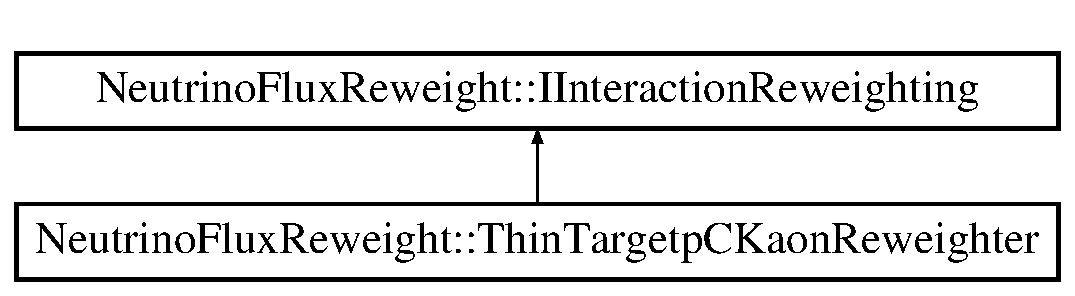
\includegraphics[height=2.000000cm]{class_neutrino_flux_reweight_1_1_thin_targetp_c_kaon_reweighter}
\end{center}
\end{figure}
\subsection*{Public Member Functions}
\begin{DoxyCompactItemize}
\item 
\hyperlink{class_neutrino_flux_reweight_1_1_thin_targetp_c_kaon_reweighter_a00eeb5526f6f7af21035e70c8bee17d1}{Thin\-Targetp\-C\-Kaon\-Reweighter} (int iuniv, const \hyperlink{class_neutrino_flux_reweight_1_1_parameter_table}{Parameter\-Table} \&cv\-\_\-pars, const \hyperlink{class_neutrino_flux_reweight_1_1_parameter_table}{Parameter\-Table} \&univ\-\_\-pars)
\item 
virtual \hyperlink{class_neutrino_flux_reweight_1_1_thin_targetp_c_kaon_reweighter_ae7931d91d1e743fe87d8b3862a11b37f}{$\sim$\-Thin\-Targetp\-C\-Kaon\-Reweighter} ()
\item 
virtual bool \hyperlink{class_neutrino_flux_reweight_1_1_thin_targetp_c_kaon_reweighter_a78d9307c378b36d660feb54ba8114a9a}{can\-Reweight} (const \hyperlink{class_neutrino_flux_reweight_1_1_interaction_data}{Interaction\-Data} \&aa)
\begin{DoxyCompactList}\small\item\em can the particular instance of this class reweight this interaction? \end{DoxyCompactList}\item 
virtual double \hyperlink{class_neutrino_flux_reweight_1_1_thin_targetp_c_kaon_reweighter_a64f5f6df3b44240b56b863206773ca9a}{calculate\-Weight} (const \hyperlink{class_neutrino_flux_reweight_1_1_interaction_data}{Interaction\-Data} \&aa)
\begin{DoxyCompactList}\small\item\em calculate a weight for this interaction given the central value parameters and the parameters for this universe. The weight is something like\-: f(cv)/f(M\-C) $\ast$ f(univ)/f(cv) where cv in this case corresponds to the best value of the parameter, given the data. If univ\-\_\-pars=cv\-\_\-pars then we are calculating a central value weight \end{DoxyCompactList}\item 
double \hyperlink{class_neutrino_flux_reweight_1_1_thin_targetp_c_kaon_reweighter_a60ee6eb8b7a376145a4ec0780a0d812d}{calculate\-Data\-Scale} (int inc\-\_\-pdg, double inc\-\_\-mom, int prod\-\_\-pdg, double xf, double pt)
\end{DoxyCompactItemize}
\subsection*{Public Attributes}
\begin{DoxyCompactItemize}
\item 
double \hyperlink{class_neutrino_flux_reweight_1_1_thin_targetp_c_kaon_reweighter_ae26e9fbd1c42a53759a1587a3312a4fb}{data\-\_\-prod\-\_\-xs}
\item 
std\-::vector$<$ float $>$ \hyperlink{class_neutrino_flux_reweight_1_1_thin_targetp_c_kaon_reweighter_a7e9b49e61de648fbe1198c3ae68ce15f}{vbin\-\_\-data\-\_\-kap}
\item 
std\-::vector$<$ float $>$ \hyperlink{class_neutrino_flux_reweight_1_1_thin_targetp_c_kaon_reweighter_afdc746047f72743b45affc7f51f8ba3f}{vbin\-\_\-data\-\_\-kam}
\item 
std\-::vector$<$ float $>$ \hyperlink{class_neutrino_flux_reweight_1_1_thin_targetp_c_kaon_reweighter_a6ad9b6cccb6fc522708b1aa5b9070c71}{mipp\-\_\-vbin\-\_\-data\-\_\-kap\-\_\-pip}
\item 
std\-::vector$<$ float $>$ \hyperlink{class_neutrino_flux_reweight_1_1_thin_targetp_c_kaon_reweighter_ab268b6554b6abe96854cec82f336816d}{mipp\-\_\-vbin\-\_\-data\-\_\-kam\-\_\-pim}
\end{DoxyCompactItemize}
\subsection*{Private Attributes}
\begin{DoxyCompactItemize}
\item 
int \hyperlink{class_neutrino_flux_reweight_1_1_thin_targetp_c_kaon_reweighter_a3ff9d5c19007a8272c69e15cc3c7742b}{i\-Univ}
\item 
const \hyperlink{class_neutrino_flux_reweight_1_1_parameter_table}{Parameter\-Table} \& \hyperlink{class_neutrino_flux_reweight_1_1_thin_targetp_c_kaon_reweighter_a474281c2bfbea82f8ddfad0cab1f1146}{cv\-Pars}
\item 
const \hyperlink{class_neutrino_flux_reweight_1_1_parameter_table}{Parameter\-Table} \& \hyperlink{class_neutrino_flux_reweight_1_1_thin_targetp_c_kaon_reweighter_a09bb649b2bc0b55691bcd9bc1228536b}{univ\-Pars}
\item 
\hyperlink{class_neutrino_flux_reweight_1_1_thin_targetp_c_pion_reweighter}{Thin\-Targetp\-C\-Pion\-Reweighter} $\ast$ \hyperlink{class_neutrino_flux_reweight_1_1_thin_targetp_c_kaon_reweighter_ab6dbf86a7f242f29d1f4e67bf1dc7e2f}{tt\-\_\-p\-C\-Pion\-Rew}
\end{DoxyCompactItemize}


\subsection{Detailed Description}
Reweighter of thin target K production. 

Definition at line 16 of file Thin\-Targetp\-C\-Kaon\-Reweighter.\-h.



\subsection{Constructor \& Destructor Documentation}
\hypertarget{class_neutrino_flux_reweight_1_1_thin_targetp_c_kaon_reweighter_a00eeb5526f6f7af21035e70c8bee17d1}{\index{Neutrino\-Flux\-Reweight\-::\-Thin\-Targetp\-C\-Kaon\-Reweighter@{Neutrino\-Flux\-Reweight\-::\-Thin\-Targetp\-C\-Kaon\-Reweighter}!Thin\-Targetp\-C\-Kaon\-Reweighter@{Thin\-Targetp\-C\-Kaon\-Reweighter}}
\index{Thin\-Targetp\-C\-Kaon\-Reweighter@{Thin\-Targetp\-C\-Kaon\-Reweighter}!NeutrinoFluxReweight::ThinTargetpCKaonReweighter@{Neutrino\-Flux\-Reweight\-::\-Thin\-Targetp\-C\-Kaon\-Reweighter}}
\subsubsection[{Thin\-Targetp\-C\-Kaon\-Reweighter}]{\setlength{\rightskip}{0pt plus 5cm}Neutrino\-Flux\-Reweight\-::\-Thin\-Targetp\-C\-Kaon\-Reweighter\-::\-Thin\-Targetp\-C\-Kaon\-Reweighter (
\begin{DoxyParamCaption}
\item[{int}]{iuniv, }
\item[{const {\bf Parameter\-Table} \&}]{cv\-\_\-pars, }
\item[{const {\bf Parameter\-Table} \&}]{univ\-\_\-pars}
\end{DoxyParamCaption}
)}}\label{class_neutrino_flux_reweight_1_1_thin_targetp_c_kaon_reweighter_a00eeb5526f6f7af21035e70c8bee17d1}


Definition at line 10 of file Thin\-Targetp\-C\-Kaon\-Reweighter.\-cpp.


\begin{DoxyCode}
10                                                                                                            
                            :\hyperlink{class_neutrino_flux_reweight_1_1_thin_targetp_c_kaon_reweighter_a3ff9d5c19007a8272c69e15cc3c7742b}{iUniv}(iuniv),\hyperlink{class_neutrino_flux_reweight_1_1_thin_targetp_c_kaon_reweighter_a474281c2bfbea82f8ddfad0cab1f1146}{cvPars}(cv\_pars),\hyperlink{class_neutrino_flux_reweight_1_1_thin_targetp_c_kaon_reweighter_a09bb649b2bc0b55691bcd9bc1228536b}{univPars}(univ\_pars)\{
11   
12     ThinTargetBins* Thinbins =  \hyperlink{class_neutrino_flux_reweight_1_1_thin_target_bins_aeff5cf7220dd08322f5abac2cbc7ff33}{ThinTargetBins::getInstance}();
13     \hyperlink{class_neutrino_flux_reweight_1_1_thin_targetp_c_kaon_reweighter_a7e9b49e61de648fbe1198c3ae68ce15f}{vbin\_data\_kap}.reserve(Thinbins->GetNbins\_pC\_KX\_NA49());
14     \hyperlink{class_neutrino_flux_reweight_1_1_thin_targetp_c_kaon_reweighter_afdc746047f72743b45affc7f51f8ba3f}{vbin\_data\_kam}.reserve(Thinbins->GetNbins\_pC\_KX\_NA49());
15     \hyperlink{class_neutrino_flux_reweight_1_1_thin_targetp_c_kaon_reweighter_a6ad9b6cccb6fc522708b1aa5b9070c71}{mipp\_vbin\_data\_kap\_pip}.reserve(Thinbins->GetNbins\_pC\_KX\_MIPP());
16     \hyperlink{class_neutrino_flux_reweight_1_1_thin_targetp_c_kaon_reweighter_ab268b6554b6abe96854cec82f336816d}{mipp\_vbin\_data\_kam\_pim}.reserve(Thinbins->GetNbins\_pC\_KX\_MIPP());
17 
18     \textcolor{comment}{// const boost::interprocess::flat\_map<std::string, double>& cv\_table   = cvPars.getMap();}
19     \textcolor{comment}{// const boost::interprocess::flat\_map<std::string, double>& univ\_table = univPars.getMap();}
20        
21     \hyperlink{class_neutrino_flux_reweight_1_1_thin_targetp_c_kaon_reweighter_ae26e9fbd1c42a53759a1587a3312a4fb}{data\_prod\_xs} = \hyperlink{class_neutrino_flux_reweight_1_1_thin_targetp_c_kaon_reweighter_a09bb649b2bc0b55691bcd9bc1228536b}{univPars}.\hyperlink{class_neutrino_flux_reweight_1_1_parameter_table_acb7dc8335b65b116f6092f2fa57ca5ed}{getParameterValue}(\textcolor{stringliteral}{"prod\_prtC\_xsec"});
22     \textcolor{keywordtype}{char} namepar[100];
23     \textcolor{keywordflow}{for}(\textcolor{keywordtype}{int} ii=0;ii<Thinbins->GetNbins\_pC\_KX\_NA49();ii++)\{
24       
25       sprintf(namepar,\textcolor{stringliteral}{"ThinTargetLowxF\_pC\_%s\_sys\_%d"},\textcolor{stringliteral}{"kap"},ii);
26       \textcolor{keywordtype}{double} data\_cv  = \hyperlink{class_neutrino_flux_reweight_1_1_thin_targetp_c_kaon_reweighter_a474281c2bfbea82f8ddfad0cab1f1146}{cvPars}.\hyperlink{class_neutrino_flux_reweight_1_1_parameter_table_acb7dc8335b65b116f6092f2fa57ca5ed}{getParameterValue}(std::string(namepar));
27       \textcolor{keywordtype}{double} data\_sys = \hyperlink{class_neutrino_flux_reweight_1_1_thin_targetp_c_kaon_reweighter_a09bb649b2bc0b55691bcd9bc1228536b}{univPars}.\hyperlink{class_neutrino_flux_reweight_1_1_parameter_table_acb7dc8335b65b116f6092f2fa57ca5ed}{getParameterValue}(std::string(namepar));
28       sprintf(namepar,\textcolor{stringliteral}{"ThinTargetLowxF\_pC\_%s\_stats\_%d"},\textcolor{stringliteral}{"kap"},ii);
29       \textcolor{keywordtype}{double} data\_sta = \hyperlink{class_neutrino_flux_reweight_1_1_thin_targetp_c_kaon_reweighter_a09bb649b2bc0b55691bcd9bc1228536b}{univPars}.\hyperlink{class_neutrino_flux_reweight_1_1_parameter_table_acb7dc8335b65b116f6092f2fa57ca5ed}{getParameterValue}(std::string(namepar));
30       \hyperlink{class_neutrino_flux_reweight_1_1_thin_targetp_c_kaon_reweighter_a7e9b49e61de648fbe1198c3ae68ce15f}{vbin\_data\_kap}.push\_back(data\_sta + data\_sys - data\_cv);
31       
32       sprintf(namepar,\textcolor{stringliteral}{"ThinTargetLowxF\_pC\_%s\_sys\_%d"},\textcolor{stringliteral}{"kam"},ii);
33       data\_cv  = \hyperlink{class_neutrino_flux_reweight_1_1_thin_targetp_c_kaon_reweighter_a474281c2bfbea82f8ddfad0cab1f1146}{cvPars}.\hyperlink{class_neutrino_flux_reweight_1_1_parameter_table_acb7dc8335b65b116f6092f2fa57ca5ed}{getParameterValue}(std::string(namepar));
34       data\_sys = \hyperlink{class_neutrino_flux_reweight_1_1_thin_targetp_c_kaon_reweighter_a09bb649b2bc0b55691bcd9bc1228536b}{univPars}.\hyperlink{class_neutrino_flux_reweight_1_1_parameter_table_acb7dc8335b65b116f6092f2fa57ca5ed}{getParameterValue}(std::string(namepar));
35       sprintf(namepar,\textcolor{stringliteral}{"ThinTargetLowxF\_pC\_%s\_stats\_%d"},\textcolor{stringliteral}{"kam"},ii);
36       data\_sta = \hyperlink{class_neutrino_flux_reweight_1_1_thin_targetp_c_kaon_reweighter_a09bb649b2bc0b55691bcd9bc1228536b}{univPars}.\hyperlink{class_neutrino_flux_reweight_1_1_parameter_table_acb7dc8335b65b116f6092f2fa57ca5ed}{getParameterValue}(std::string(namepar));
37       \hyperlink{class_neutrino_flux_reweight_1_1_thin_targetp_c_kaon_reweighter_afdc746047f72743b45affc7f51f8ba3f}{vbin\_data\_kam}.push\_back(data\_sta + data\_sys - data\_cv);
38       
39     \}
40     
41     \textcolor{keywordflow}{for}(\textcolor{keywordtype}{int} ii=0;ii<Thinbins->GetNbins\_pC\_KX\_MIPP();ii++)\{
42       
43       sprintf(namepar,\textcolor{stringliteral}{"ThinTarget\_kap\_pip\_sys\_%d"},ii);
44       \textcolor{keywordtype}{double} data\_cv  = \hyperlink{class_neutrino_flux_reweight_1_1_thin_targetp_c_kaon_reweighter_a474281c2bfbea82f8ddfad0cab1f1146}{cvPars}.\hyperlink{class_neutrino_flux_reweight_1_1_parameter_table_acb7dc8335b65b116f6092f2fa57ca5ed}{getParameterValue}(std::string(namepar));
45       \textcolor{keywordtype}{double} data\_sys = \hyperlink{class_neutrino_flux_reweight_1_1_thin_targetp_c_kaon_reweighter_a09bb649b2bc0b55691bcd9bc1228536b}{univPars}.\hyperlink{class_neutrino_flux_reweight_1_1_parameter_table_acb7dc8335b65b116f6092f2fa57ca5ed}{getParameterValue}(std::string(namepar));
46       sprintf(namepar,\textcolor{stringliteral}{"ThinTarget\_kap\_pip\_stats\_%d"},ii);
47       \textcolor{keywordtype}{double} data\_sta = \hyperlink{class_neutrino_flux_reweight_1_1_thin_targetp_c_kaon_reweighter_a09bb649b2bc0b55691bcd9bc1228536b}{univPars}.\hyperlink{class_neutrino_flux_reweight_1_1_parameter_table_acb7dc8335b65b116f6092f2fa57ca5ed}{getParameterValue}(std::string(namepar));
48       \hyperlink{class_neutrino_flux_reweight_1_1_thin_targetp_c_kaon_reweighter_a6ad9b6cccb6fc522708b1aa5b9070c71}{mipp\_vbin\_data\_kap\_pip}.push\_back(data\_sta + data\_sys - data\_cv);
49 
50       sprintf(namepar,\textcolor{stringliteral}{"ThinTarget\_kam\_pim\_sys\_%d"},ii);
51       data\_cv  = \hyperlink{class_neutrino_flux_reweight_1_1_thin_targetp_c_kaon_reweighter_a474281c2bfbea82f8ddfad0cab1f1146}{cvPars}.\hyperlink{class_neutrino_flux_reweight_1_1_parameter_table_acb7dc8335b65b116f6092f2fa57ca5ed}{getParameterValue}(std::string(namepar));
52       data\_sys = \hyperlink{class_neutrino_flux_reweight_1_1_thin_targetp_c_kaon_reweighter_a09bb649b2bc0b55691bcd9bc1228536b}{univPars}.\hyperlink{class_neutrino_flux_reweight_1_1_parameter_table_acb7dc8335b65b116f6092f2fa57ca5ed}{getParameterValue}(std::string(namepar));
53       sprintf(namepar,\textcolor{stringliteral}{"ThinTarget\_kam\_pim\_stats\_%d"},ii);
54       data\_sta = \hyperlink{class_neutrino_flux_reweight_1_1_thin_targetp_c_kaon_reweighter_a09bb649b2bc0b55691bcd9bc1228536b}{univPars}.\hyperlink{class_neutrino_flux_reweight_1_1_parameter_table_acb7dc8335b65b116f6092f2fa57ca5ed}{getParameterValue}(std::string(namepar));
55       \hyperlink{class_neutrino_flux_reweight_1_1_thin_targetp_c_kaon_reweighter_ab268b6554b6abe96854cec82f336816d}{mipp\_vbin\_data\_kam\_pim}.push\_back(data\_sta + data\_sys - data\_cv);
56 
57     \} 
58     
59   \}
\end{DoxyCode}
\hypertarget{class_neutrino_flux_reweight_1_1_thin_targetp_c_kaon_reweighter_ae7931d91d1e743fe87d8b3862a11b37f}{\index{Neutrino\-Flux\-Reweight\-::\-Thin\-Targetp\-C\-Kaon\-Reweighter@{Neutrino\-Flux\-Reweight\-::\-Thin\-Targetp\-C\-Kaon\-Reweighter}!$\sim$\-Thin\-Targetp\-C\-Kaon\-Reweighter@{$\sim$\-Thin\-Targetp\-C\-Kaon\-Reweighter}}
\index{$\sim$\-Thin\-Targetp\-C\-Kaon\-Reweighter@{$\sim$\-Thin\-Targetp\-C\-Kaon\-Reweighter}!NeutrinoFluxReweight::ThinTargetpCKaonReweighter@{Neutrino\-Flux\-Reweight\-::\-Thin\-Targetp\-C\-Kaon\-Reweighter}}
\subsubsection[{$\sim$\-Thin\-Targetp\-C\-Kaon\-Reweighter}]{\setlength{\rightskip}{0pt plus 5cm}Neutrino\-Flux\-Reweight\-::\-Thin\-Targetp\-C\-Kaon\-Reweighter\-::$\sim$\-Thin\-Targetp\-C\-Kaon\-Reweighter (
\begin{DoxyParamCaption}
{}
\end{DoxyParamCaption}
)\hspace{0.3cm}{\ttfamily [virtual]}}}\label{class_neutrino_flux_reweight_1_1_thin_targetp_c_kaon_reweighter_ae7931d91d1e743fe87d8b3862a11b37f}


Definition at line 61 of file Thin\-Targetp\-C\-Kaon\-Reweighter.\-cpp.


\begin{DoxyCode}
61                                                          \{
62     
63   \}
\end{DoxyCode}


\subsection{Member Function Documentation}
\hypertarget{class_neutrino_flux_reweight_1_1_thin_targetp_c_kaon_reweighter_a60ee6eb8b7a376145a4ec0780a0d812d}{\index{Neutrino\-Flux\-Reweight\-::\-Thin\-Targetp\-C\-Kaon\-Reweighter@{Neutrino\-Flux\-Reweight\-::\-Thin\-Targetp\-C\-Kaon\-Reweighter}!calculate\-Data\-Scale@{calculate\-Data\-Scale}}
\index{calculate\-Data\-Scale@{calculate\-Data\-Scale}!NeutrinoFluxReweight::ThinTargetpCKaonReweighter@{Neutrino\-Flux\-Reweight\-::\-Thin\-Targetp\-C\-Kaon\-Reweighter}}
\subsubsection[{calculate\-Data\-Scale}]{\setlength{\rightskip}{0pt plus 5cm}double Neutrino\-Flux\-Reweight\-::\-Thin\-Targetp\-C\-Kaon\-Reweighter\-::calculate\-Data\-Scale (
\begin{DoxyParamCaption}
\item[{int}]{inc\-\_\-pdg, }
\item[{double}]{inc\-\_\-mom, }
\item[{int}]{prod\-\_\-pdg, }
\item[{double}]{xf, }
\item[{double}]{pt}
\end{DoxyParamCaption}
)}}\label{class_neutrino_flux_reweight_1_1_thin_targetp_c_kaon_reweighter_a60ee6eb8b7a376145a4ec0780a0d812d}


Definition at line 204 of file Thin\-Targetp\-C\-Kaon\-Reweighter.\-cpp.


\begin{DoxyCode}
204                                                                                                            
                \{
205     \textcolor{keywordtype}{double} scaling\_violation = 1.0;
206     ThinTargetMC*  dtH =  \hyperlink{class_neutrino_flux_reweight_1_1_thin_target_m_c_a2a114747fed2677cd3b7213555c002b9}{ThinTargetMC::getInstance}();
207     \textcolor{comment}{//temporary:}
208     \textcolor{keyword}{const} \textcolor{keywordtype}{int} Nscl = 11;
209     \textcolor{keyword}{const} \textcolor{keywordtype}{int} moms[Nscl] = \{12,20,31,40,50,60,70,80,100,120,158\};
210     
211     \textcolor{keywordtype}{int} idx\_part = -1;
212     \textcolor{keywordflow}{if}(prod\_pdg == 321)idx\_part = 2;
213     \textcolor{keywordflow}{if}(prod\_pdg ==-321)idx\_part = 3;
214     \textcolor{keywordflow}{if}(idx\_part<0)\{
215       std::cout<<\textcolor{stringliteral}{"Error in the prod particle"}<<std::endl;
216       \textcolor{keywordflow}{return} 1.0;
217     \}
218     
219     \textcolor{keywordtype}{int} binid = dtH->hTTScl[idx\_part][Nscl-1]->FindBin(xf,pt);
220     \textcolor{keywordtype}{double} scl\_ref158 = dtH->hTTScl[idx\_part][Nscl-1]->GetBinContent(binid);    
221     
222     \textcolor{keywordtype}{int} idx\_lowp = -1;
223     \textcolor{keywordtype}{int} idx\_hip  = -1;
224     \textcolor{keywordflow}{for}(\textcolor{keywordtype}{int} i=0;i<Nscl-1;i++)\{
225       \textcolor{keywordflow}{if}(inc\_mom>=\textcolor{keywordtype}{double}(moms[i]) && inc\_mom<\textcolor{keywordtype}{double}(moms[i+1]))\{
226         idx\_lowp=i;
227         idx\_hip =i+1;
228       \}
229     \}
230     \textcolor{keywordflow}{if}(idx\_lowp<0 || idx\_hip<0)\{
231       std::cout<<\textcolor{stringliteral}{"Error calculating the scaling"}<<std::endl;
232       \textcolor{keywordflow}{return} 1.0;
233     \}
234     \textcolor{keywordtype}{double} scl\_low = dtH->hTTScl[idx\_part][idx\_lowp]->GetBinContent(binid);
235     \textcolor{keywordtype}{double} scl\_hi  = dtH->hTTScl[idx\_part][idx\_hip]->GetBinContent(binid);
236     \textcolor{keywordtype}{double} scl\_m   =  scl\_low + (inc\_mom-double(moms[idx\_lowp]))*(scl\_hi-scl\_low)/(double(moms[idx\_hip])-
      double(moms[idx\_lowp]));
237     \textcolor{keywordflow}{if}(scl\_ref158<1.e-10)\{
238       \textcolor{comment}{// std::cout<<"ref158 zero!!! "<<scl\_ref158<<std::endl;}
239       \textcolor{keywordflow}{return} 1.0;
240     \}
241     scaling\_violation = scl\_m/scl\_ref158;
242     \textcolor{keywordflow}{return} scaling\_violation;
243   \}
\end{DoxyCode}
\hypertarget{class_neutrino_flux_reweight_1_1_thin_targetp_c_kaon_reweighter_a64f5f6df3b44240b56b863206773ca9a}{\index{Neutrino\-Flux\-Reweight\-::\-Thin\-Targetp\-C\-Kaon\-Reweighter@{Neutrino\-Flux\-Reweight\-::\-Thin\-Targetp\-C\-Kaon\-Reweighter}!calculate\-Weight@{calculate\-Weight}}
\index{calculate\-Weight@{calculate\-Weight}!NeutrinoFluxReweight::ThinTargetpCKaonReweighter@{Neutrino\-Flux\-Reweight\-::\-Thin\-Targetp\-C\-Kaon\-Reweighter}}
\subsubsection[{calculate\-Weight}]{\setlength{\rightskip}{0pt plus 5cm}double Neutrino\-Flux\-Reweight\-::\-Thin\-Targetp\-C\-Kaon\-Reweighter\-::calculate\-Weight (
\begin{DoxyParamCaption}
\item[{const {\bf Interaction\-Data} \&}]{inter\-\_\-data}
\end{DoxyParamCaption}
)\hspace{0.3cm}{\ttfamily [virtual]}}}\label{class_neutrino_flux_reweight_1_1_thin_targetp_c_kaon_reweighter_a64f5f6df3b44240b56b863206773ca9a}


calculate a weight for this interaction given the central value parameters and the parameters for this universe. The weight is something like\-: f(cv)/f(M\-C) $\ast$ f(univ)/f(cv) where cv in this case corresponds to the best value of the parameter, given the data. If univ\-\_\-pars=cv\-\_\-pars then we are calculating a central value weight 



Implements \hyperlink{class_neutrino_flux_reweight_1_1_i_interaction_reweighting_a49b0d73e778411d629205d23575703c3}{Neutrino\-Flux\-Reweight\-::\-I\-Interaction\-Reweighting}.



Definition at line 109 of file Thin\-Targetp\-C\-Kaon\-Reweighter.\-cpp.


\begin{DoxyCode}
109                                                                              \{
110     
111     \textcolor{keywordtype}{double} wgt = 1.0;
112 
113     ThinTargetBins*  Thinbins =  \hyperlink{class_neutrino_flux_reweight_1_1_thin_target_bins_aeff5cf7220dd08322f5abac2cbc7ff33}{ThinTargetBins::getInstance}();
114     \textcolor{keywordtype}{int} bin      = Thinbins->BinID\_pC\_k(aa.xF,aa.Pt,aa.Prod\_pdg);
115     \textcolor{keywordtype}{int} mipp\_bin = Thinbins->mipp\_BinID\_pC\_k(aa.Pz,aa.Pt,aa.Prod\_pdg);
116     \textcolor{keywordflow}{if}(bin<0 && mipp\_bin<0)\textcolor{keywordflow}{return} wgt;  \textcolor{comment}{//double check}
117     
118     \textcolor{keywordtype}{double} dataval = -1;
119     
120     \textcolor{keywordflow}{if}(bin>=0)\{
121       \textcolor{keywordflow}{if}(aa.Prod\_pdg == 321)dataval = \hyperlink{class_neutrino_flux_reweight_1_1_thin_targetp_c_kaon_reweighter_a7e9b49e61de648fbe1198c3ae68ce15f}{vbin\_data\_kap}[bin];
122       \textcolor{keywordflow}{else} \textcolor{keywordflow}{if}(aa.Prod\_pdg == -321) dataval = \hyperlink{class_neutrino_flux_reweight_1_1_thin_targetp_c_kaon_reweighter_afdc746047f72743b45affc7f51f8ba3f}{vbin\_data\_kam}[bin];
123       \textcolor{keywordflow}{else} \textcolor{keywordflow}{if}(aa.Prod\_pdg == 130 || aa.Prod\_pdg == 310)\{
124         dataval = 0.25*(\hyperlink{class_neutrino_flux_reweight_1_1_thin_targetp_c_kaon_reweighter_a7e9b49e61de648fbe1198c3ae68ce15f}{vbin\_data\_kap}[bin]+3.*\hyperlink{class_neutrino_flux_reweight_1_1_thin_targetp_c_kaon_reweighter_afdc746047f72743b45affc7f51f8ba3f}{vbin\_data\_kam}[bin]);
125       \}
126       \textcolor{keywordflow}{else}\{
127         std::cout<<\textcolor{stringliteral}{"Something is wrong, pdg\_prod: "}<< aa.Prod\_pdg  <<std::endl;
128         \textcolor{keywordflow}{return} wgt;
129       \}
130     \}
131     \textcolor{keywordflow}{else} \textcolor{keywordflow}{if}(mipp\_bin>=0)\{
132    
133       MakeReweight*  makerew =  \hyperlink{class_neutrino_flux_reweight_1_1_make_reweight_a42d1fa92a1e30bd80538188e0c9d8b4a}{MakeReweight::getInstance}();
134       \textcolor{keywordflow}{if}(\hyperlink{class_neutrino_flux_reweight_1_1_thin_targetp_c_kaon_reweighter_a3ff9d5c19007a8272c69e15cc3c7742b}{iUniv}==-1)\hyperlink{class_neutrino_flux_reweight_1_1_thin_targetp_c_kaon_reweighter_ab6dbf86a7f242f29d1f4e67bf1dc7e2f}{tt\_pCPionRew} = (makerew->cv\_rw)->THINTARGET\_PC\_PION\_Universe;
135       \textcolor{keywordflow}{else} \hyperlink{class_neutrino_flux_reweight_1_1_thin_targetp_c_kaon_reweighter_ab6dbf86a7f242f29d1f4e67bf1dc7e2f}{tt\_pCPionRew} = (makerew->vec\_rws[\hyperlink{class_neutrino_flux_reweight_1_1_thin_targetp_c_kaon_reweighter_a3ff9d5c19007a8272c69e15cc3c7742b}{iUniv}])->THINTARGET\_PC\_PION\_Universe; 
136       
137       \textcolor{keywordtype}{double} inc\_mom[3]  = \{aa.Inc\_P4[0], aa.Inc\_P4[1], aa.Inc\_P4[2]\};
138       \textcolor{keywordtype}{double} prod\_mom[3] = \{aa.Prod\_P4[0],aa.Prod\_P4[1],aa.Prod\_P4[2]\};
139       \textcolor{keywordtype}{double} vtx\_int[3]  = \{aa.Vtx[0],aa.Vtx[1],aa.Vtx[2]\};
140       \textcolor{keywordtype}{double} pip\_data = -1.0; 
141       \textcolor{keywordtype}{double} pim\_data = -1.0; 
142       \textcolor{keywordtype}{int} bin\_pi = -1;
143       InteractionData aux\_aa(aa.gen, inc\_mom,2212,prod\_mom,211,aa.Vol,aa.Proc,vtx\_int);    
144       \textcolor{keywordflow}{if}(aux\_aa.xF<=0.5)\{
145         bin\_pi = Thinbins->BinID\_pC\_pi(aux\_aa.xF,aux\_aa.Pt,aux\_aa.Prod\_pdg);
146         \textcolor{keywordflow}{if}(bin\_pi<0)\textcolor{keywordflow}{return} 1.0;
147         pip\_data = \hyperlink{class_neutrino_flux_reweight_1_1_thin_targetp_c_kaon_reweighter_ab6dbf86a7f242f29d1f4e67bf1dc7e2f}{tt\_pCPionRew}->\hyperlink{class_neutrino_flux_reweight_1_1_thin_targetp_c_pion_reweighter_a3602ae8237c0cc7729045b13b90874b4}{vbin\_data\_pip}[bin\_pi];
148         pim\_data = \hyperlink{class_neutrino_flux_reweight_1_1_thin_targetp_c_kaon_reweighter_ab6dbf86a7f242f29d1f4e67bf1dc7e2f}{tt\_pCPionRew}->\hyperlink{class_neutrino_flux_reweight_1_1_thin_targetp_c_pion_reweighter_aea0dca1b93e560e26871da0bdf1ac075}{vbin\_data\_pim}[bin\_pi];        
149       \}
150       \textcolor{keywordflow}{else} \textcolor{keywordflow}{if}(aux\_aa.xF>0.5)\{
151         bin\_pi = Thinbins->barton\_BinID\_pC\_pi(aux\_aa.xF,aux\_aa.Pt,aux\_aa.Prod\_pdg);
152         \textcolor{keywordflow}{if}(bin\_pi<0)\textcolor{keywordflow}{return} 1.0;
153         pip\_data = \hyperlink{class_neutrino_flux_reweight_1_1_thin_targetp_c_kaon_reweighter_ab6dbf86a7f242f29d1f4e67bf1dc7e2f}{tt\_pCPionRew}->\hyperlink{class_neutrino_flux_reweight_1_1_thin_targetp_c_pion_reweighter_a844e9c7ba521a42ce5ebe5fbb5b2d5f4}{bart\_vbin\_data\_pip}[bin\_pi];
154         pim\_data = \hyperlink{class_neutrino_flux_reweight_1_1_thin_targetp_c_kaon_reweighter_ab6dbf86a7f242f29d1f4e67bf1dc7e2f}{tt\_pCPionRew}->\hyperlink{class_neutrino_flux_reweight_1_1_thin_targetp_c_pion_reweighter_a9d7ffcf3ca0c5a7b0f1c37435cc86403}{bart\_vbin\_data\_pim}[bin\_pi];      
155       \}
156 
157       \textcolor{keywordflow}{if}(aa.Prod\_pdg == 321)\{
158         dataval = \hyperlink{class_neutrino_flux_reweight_1_1_thin_targetp_c_kaon_reweighter_a6ad9b6cccb6fc522708b1aa5b9070c71}{mipp\_vbin\_data\_kap\_pip}[mipp\_bin]*pip\_data;
159       \}
160       \textcolor{keywordflow}{else} \textcolor{keywordflow}{if}(aa.Prod\_pdg ==-321)\{
161         dataval = \hyperlink{class_neutrino_flux_reweight_1_1_thin_targetp_c_kaon_reweighter_ab268b6554b6abe96854cec82f336816d}{mipp\_vbin\_data\_kam\_pim}[mipp\_bin]*pim\_data;
162       \}
163       \textcolor{keywordflow}{else} \textcolor{keywordflow}{if}(aa.Prod\_pdg == 130 || aa.Prod\_pdg == 310)\{
164         dataval = 0.25*(\hyperlink{class_neutrino_flux_reweight_1_1_thin_targetp_c_kaon_reweighter_a6ad9b6cccb6fc522708b1aa5b9070c71}{mipp\_vbin\_data\_kap\_pip}[mipp\_bin]*pip\_data +3.0*(
      \hyperlink{class_neutrino_flux_reweight_1_1_thin_targetp_c_kaon_reweighter_ab268b6554b6abe96854cec82f336816d}{mipp\_vbin\_data\_kam\_pim}[mipp\_bin]*pim\_data));
165       \}
166     \}
167          
168     \textcolor{comment}{//checking if this is the first interaction:}
169     \textcolor{keywordflow}{if}(aa.gen==0)dataval /= \hyperlink{class_neutrino_flux_reweight_1_1_thin_targetp_c_kaon_reweighter_ae26e9fbd1c42a53759a1587a3312a4fb}{data\_prod\_xs};
170     \textcolor{keywordflow}{else} \textcolor{keywordflow}{if}(aa.gen>0)dataval /= 1.0;
171     \textcolor{keywordflow}{else}\{
172       std::cout<<\textcolor{stringliteral}{"Something is wrong with gen "}<<std::endl;
173       \textcolor{keywordflow}{return} wgt;
174     \}
175 
176     \textcolor{keywordtype}{double} data\_scale = -1.0;
177     \textcolor{keywordflow}{if}(aa.Prod\_pdg == 321 || aa.Prod\_pdg == -321)\{
178       data\_scale = \hyperlink{class_neutrino_flux_reweight_1_1_thin_targetp_c_kaon_reweighter_a60ee6eb8b7a376145a4ec0780a0d812d}{calculateDataScale}(aa.Inc\_pdg,aa.Inc\_P,aa.Prod\_pdg,aa.xF,aa.Pt);   
179     \}
180     \textcolor{keywordflow}{else} \textcolor{keywordflow}{if}(aa.Prod\_pdg == 130 || aa.Prod\_pdg == 310)\{
181       data\_scale = 0.25*(\hyperlink{class_neutrino_flux_reweight_1_1_thin_targetp_c_kaon_reweighter_a60ee6eb8b7a376145a4ec0780a0d812d}{calculateDataScale}(aa.Inc\_pdg,aa.Inc\_P,321,aa.xF,aa.Pt)+3.*
      \hyperlink{class_neutrino_flux_reweight_1_1_thin_targetp_c_kaon_reweighter_a60ee6eb8b7a376145a4ec0780a0d812d}{calculateDataScale}(aa.Inc\_pdg,aa.Inc\_P,-321,aa.xF,aa.Pt));  
182       
183     \}
184     dataval *= data\_scale;
185 
186     ThinTargetMC*  mc =  \hyperlink{class_neutrino_flux_reweight_1_1_thin_target_m_c_a2a114747fed2677cd3b7213555c002b9}{ThinTargetMC::getInstance}();
187     \textcolor{keywordtype}{double} mc\_cv   = mc->getMCval\_pC\_X(aa.Inc\_P,aa.xF,aa.Pt,aa.Prod\_pdg);
188     \textcolor{keywordtype}{double} mc\_prod = mc->getMCxs\_pC\_piK(aa.gen,aa.Inc\_P);
189 
190     mc\_cv /= mc\_prod;
191 
192     \textcolor{keywordflow}{if}(mc\_cv<1.e-12)\textcolor{keywordflow}{return} wgt;
193     wgt = dataval/mc\_cv;
194 
195     \textcolor{keywordflow}{if}(wgt<0)\{
196       \textcolor{comment}{//std::cout<<"TTPCK check wgt(<0) "<<iUniv<<" "<<aa.Inc\_P<<" "<<aa.xF<<" "<<aa.Pt<<"
       "<<aa.Prod\_pdg<<std::endl;}
197       \textcolor{keywordflow}{return} 1.0;
198     \}
199     
200     \textcolor{keywordflow}{return} wgt;
201     
202   \}
\end{DoxyCode}
\hypertarget{class_neutrino_flux_reweight_1_1_thin_targetp_c_kaon_reweighter_a78d9307c378b36d660feb54ba8114a9a}{\index{Neutrino\-Flux\-Reweight\-::\-Thin\-Targetp\-C\-Kaon\-Reweighter@{Neutrino\-Flux\-Reweight\-::\-Thin\-Targetp\-C\-Kaon\-Reweighter}!can\-Reweight@{can\-Reweight}}
\index{can\-Reweight@{can\-Reweight}!NeutrinoFluxReweight::ThinTargetpCKaonReweighter@{Neutrino\-Flux\-Reweight\-::\-Thin\-Targetp\-C\-Kaon\-Reweighter}}
\subsubsection[{can\-Reweight}]{\setlength{\rightskip}{0pt plus 5cm}bool Neutrino\-Flux\-Reweight\-::\-Thin\-Targetp\-C\-Kaon\-Reweighter\-::can\-Reweight (
\begin{DoxyParamCaption}
\item[{const {\bf Interaction\-Data} \&}]{aa}
\end{DoxyParamCaption}
)\hspace{0.3cm}{\ttfamily [virtual]}}}\label{class_neutrino_flux_reweight_1_1_thin_targetp_c_kaon_reweighter_a78d9307c378b36d660feb54ba8114a9a}


can the particular instance of this class reweight this interaction? 



Implements \hyperlink{class_neutrino_flux_reweight_1_1_i_interaction_reweighting_aa3d1d3f37a93b02e447cf5eca333ac8d}{Neutrino\-Flux\-Reweight\-::\-I\-Interaction\-Reweighting}.



Definition at line 64 of file Thin\-Targetp\-C\-Kaon\-Reweighter.\-cpp.


\begin{DoxyCode}
64                                                                        \{
65     \textcolor{comment}{//checking:}
66     std::string mode(getenv(\textcolor{stringliteral}{"MODE"}));
67     \textcolor{keywordflow}{if}(aa.Inc\_pdg != 2212)\textcolor{keywordflow}{return} \textcolor{keyword}{false};
68     \textcolor{keywordflow}{if}(aa.Inc\_P < 12.0)\textcolor{keywordflow}{return} \textcolor{keyword}{false};
69     \textcolor{comment}{//volume check: }
70     \textcolor{keywordtype}{bool} is\_wrong\_volume = aa.Vol != \textcolor{stringliteral}{"TGT1"} && aa.Vol != \textcolor{stringliteral}{"BudalMonitor"} && aa.Vol != \textcolor{stringliteral}{"Budal\_HFVS"} && aa.Vol
       != \textcolor{stringliteral}{"Budal\_VFHS"};
71     \textcolor{keywordflow}{if}( (mode==\textcolor{stringliteral}{"REF"}) || (mode==\textcolor{stringliteral}{"OPT"}) )\{
72       is\_wrong\_volume = aa.Vol != \textcolor{stringliteral}{"TargetFinHorizontal"} && aa.Vol != \textcolor{stringliteral}{"TargetNoSplitSegment"} && aa.Vol!=\textcolor{stringliteral}{"
      tCoreLog"};
73     \}
74     \textcolor{keywordflow}{if}(is\_wrong\_volume)\textcolor{keywordflow}{return} \textcolor{keyword}{false};
75     \textcolor{comment}{//}
76     \textcolor{keywordflow}{if}(aa.Prod\_pdg != 321 && aa.Prod\_pdg != -321 && aa.Prod\_pdg != 310 && aa.Prod\_pdg != 130)\textcolor{keywordflow}{return} \textcolor{keyword}{false};
77     
78     \textcolor{comment}{//Looking for low pz kaon:}
79     ThinTargetBins*  Thinbins =  \hyperlink{class_neutrino_flux_reweight_1_1_thin_target_bins_aeff5cf7220dd08322f5abac2cbc7ff33}{ThinTargetBins::getInstance}();
80     \textcolor{keywordtype}{int} bin      = Thinbins->BinID\_pC\_k(aa.xF,aa.Pt,aa.Prod\_pdg);
81     \textcolor{keywordflow}{if}(bin>=0)\textcolor{keywordflow}{return} \textcolor{keyword}{true}; \textcolor{comment}{//found NA49 kaon }
82     
83     \textcolor{comment}{//Looking for high pz kaon:}
84     \textcolor{keywordtype}{int} mipp\_bin = Thinbins->mipp\_BinID\_pC\_k(aa.Pz,aa.Pt,aa.Prod\_pdg);
85     \textcolor{keywordflow}{if}(mipp\_bin<0)\textcolor{keywordflow}{return} \textcolor{keyword}{false}; \textcolor{comment}{//no mipp thin target kaon  }
86 
87     \textcolor{keywordtype}{double} inc\_mom[3]  = \{aa.Inc\_P4[0], aa.Inc\_P4[1], aa.Inc\_P4[2]\};
88     \textcolor{keywordtype}{double} prod\_mom[3] = \{aa.Prod\_P4[0],aa.Prod\_P4[1],aa.Prod\_P4[2]\};
89     \textcolor{keywordtype}{double} vtx\_int[3]  = \{aa.Vtx[0],aa.Vtx[1],aa.Vtx[2]\};
90     
91     MakeReweight*  makerew =  \hyperlink{class_neutrino_flux_reweight_1_1_make_reweight_a42d1fa92a1e30bd80538188e0c9d8b4a}{MakeReweight::getInstance}();
92     \textcolor{keywordflow}{if}(\hyperlink{class_neutrino_flux_reweight_1_1_thin_targetp_c_kaon_reweighter_a3ff9d5c19007a8272c69e15cc3c7742b}{iUniv}==-1)\hyperlink{class_neutrino_flux_reweight_1_1_thin_targetp_c_kaon_reweighter_ab6dbf86a7f242f29d1f4e67bf1dc7e2f}{tt\_pCPionRew} = (makerew->cv\_rw)->THINTARGET\_PC\_PION\_Universe;
93     \textcolor{keywordflow}{else} \hyperlink{class_neutrino_flux_reweight_1_1_thin_targetp_c_kaon_reweighter_ab6dbf86a7f242f29d1f4e67bf1dc7e2f}{tt\_pCPionRew} = (makerew->vec\_rws[\hyperlink{class_neutrino_flux_reweight_1_1_thin_targetp_c_kaon_reweighter_a3ff9d5c19007a8272c69e15cc3c7742b}{iUniv}])->THINTARGET\_PC\_PION\_Universe;   
94 
95     InteractionData aux\_intData(aa.gen, inc\_mom,2212,prod\_mom,211,aa.Vol,aa.Proc,vtx\_int);   
96     \textcolor{keywordtype}{bool} there\_is\_pip = \hyperlink{class_neutrino_flux_reweight_1_1_thin_targetp_c_kaon_reweighter_ab6dbf86a7f242f29d1f4e67bf1dc7e2f}{tt\_pCPionRew}->\hyperlink{class_neutrino_flux_reweight_1_1_thin_targetp_c_pion_reweighter_a09067dcacb294ca133e2660d61302e85}{canReweight}(aux\_intData);    
97     
98     InteractionData aux\_intData2(aa.gen, inc\_mom,2212,prod\_mom,-211,aa.Vol,aa.Proc,vtx\_int);   
99     \textcolor{keywordtype}{bool} there\_is\_pim = \hyperlink{class_neutrino_flux_reweight_1_1_thin_targetp_c_kaon_reweighter_ab6dbf86a7f242f29d1f4e67bf1dc7e2f}{tt\_pCPionRew}->\hyperlink{class_neutrino_flux_reweight_1_1_thin_targetp_c_pion_reweighter_a09067dcacb294ca133e2660d61302e85}{canReweight}(aux\_intData2); 
100 
101     \textcolor{keywordflow}{if}(aa.Prod\_pdg == 321)\textcolor{keywordflow}{return} there\_is\_pip;
102     \textcolor{keywordflow}{else} \textcolor{keywordflow}{if}(aa.Prod\_pdg ==-321)\textcolor{keywordflow}{return} there\_is\_pim;
103     \textcolor{keywordflow}{else} \textcolor{keywordflow}{if}(aa.Prod\_pdg == 130 || aa.Prod\_pdg == 310)\textcolor{keywordflow}{return} there\_is\_pim && there\_is\_pip;
104     \textcolor{keywordflow}{else}\{
105       \textcolor{keywordflow}{return} \textcolor{keyword}{false};
106     \}
107   \}
\end{DoxyCode}


\subsection{Member Data Documentation}
\hypertarget{class_neutrino_flux_reweight_1_1_thin_targetp_c_kaon_reweighter_a474281c2bfbea82f8ddfad0cab1f1146}{\index{Neutrino\-Flux\-Reweight\-::\-Thin\-Targetp\-C\-Kaon\-Reweighter@{Neutrino\-Flux\-Reweight\-::\-Thin\-Targetp\-C\-Kaon\-Reweighter}!cv\-Pars@{cv\-Pars}}
\index{cv\-Pars@{cv\-Pars}!NeutrinoFluxReweight::ThinTargetpCKaonReweighter@{Neutrino\-Flux\-Reweight\-::\-Thin\-Targetp\-C\-Kaon\-Reweighter}}
\subsubsection[{cv\-Pars}]{\setlength{\rightskip}{0pt plus 5cm}const {\bf Parameter\-Table}\& Neutrino\-Flux\-Reweight\-::\-Thin\-Targetp\-C\-Kaon\-Reweighter\-::cv\-Pars\hspace{0.3cm}{\ttfamily [private]}}}\label{class_neutrino_flux_reweight_1_1_thin_targetp_c_kaon_reweighter_a474281c2bfbea82f8ddfad0cab1f1146}


Definition at line 30 of file Thin\-Targetp\-C\-Kaon\-Reweighter.\-h.

\hypertarget{class_neutrino_flux_reweight_1_1_thin_targetp_c_kaon_reweighter_ae26e9fbd1c42a53759a1587a3312a4fb}{\index{Neutrino\-Flux\-Reweight\-::\-Thin\-Targetp\-C\-Kaon\-Reweighter@{Neutrino\-Flux\-Reweight\-::\-Thin\-Targetp\-C\-Kaon\-Reweighter}!data\-\_\-prod\-\_\-xs@{data\-\_\-prod\-\_\-xs}}
\index{data\-\_\-prod\-\_\-xs@{data\-\_\-prod\-\_\-xs}!NeutrinoFluxReweight::ThinTargetpCKaonReweighter@{Neutrino\-Flux\-Reweight\-::\-Thin\-Targetp\-C\-Kaon\-Reweighter}}
\subsubsection[{data\-\_\-prod\-\_\-xs}]{\setlength{\rightskip}{0pt plus 5cm}double Neutrino\-Flux\-Reweight\-::\-Thin\-Targetp\-C\-Kaon\-Reweighter\-::data\-\_\-prod\-\_\-xs}}\label{class_neutrino_flux_reweight_1_1_thin_targetp_c_kaon_reweighter_ae26e9fbd1c42a53759a1587a3312a4fb}


Definition at line 23 of file Thin\-Targetp\-C\-Kaon\-Reweighter.\-h.

\hypertarget{class_neutrino_flux_reweight_1_1_thin_targetp_c_kaon_reweighter_a3ff9d5c19007a8272c69e15cc3c7742b}{\index{Neutrino\-Flux\-Reweight\-::\-Thin\-Targetp\-C\-Kaon\-Reweighter@{Neutrino\-Flux\-Reweight\-::\-Thin\-Targetp\-C\-Kaon\-Reweighter}!i\-Univ@{i\-Univ}}
\index{i\-Univ@{i\-Univ}!NeutrinoFluxReweight::ThinTargetpCKaonReweighter@{Neutrino\-Flux\-Reweight\-::\-Thin\-Targetp\-C\-Kaon\-Reweighter}}
\subsubsection[{i\-Univ}]{\setlength{\rightskip}{0pt plus 5cm}int Neutrino\-Flux\-Reweight\-::\-Thin\-Targetp\-C\-Kaon\-Reweighter\-::i\-Univ\hspace{0.3cm}{\ttfamily [private]}}}\label{class_neutrino_flux_reweight_1_1_thin_targetp_c_kaon_reweighter_a3ff9d5c19007a8272c69e15cc3c7742b}


Definition at line 29 of file Thin\-Targetp\-C\-Kaon\-Reweighter.\-h.

\hypertarget{class_neutrino_flux_reweight_1_1_thin_targetp_c_kaon_reweighter_ab268b6554b6abe96854cec82f336816d}{\index{Neutrino\-Flux\-Reweight\-::\-Thin\-Targetp\-C\-Kaon\-Reweighter@{Neutrino\-Flux\-Reweight\-::\-Thin\-Targetp\-C\-Kaon\-Reweighter}!mipp\-\_\-vbin\-\_\-data\-\_\-kam\-\_\-pim@{mipp\-\_\-vbin\-\_\-data\-\_\-kam\-\_\-pim}}
\index{mipp\-\_\-vbin\-\_\-data\-\_\-kam\-\_\-pim@{mipp\-\_\-vbin\-\_\-data\-\_\-kam\-\_\-pim}!NeutrinoFluxReweight::ThinTargetpCKaonReweighter@{Neutrino\-Flux\-Reweight\-::\-Thin\-Targetp\-C\-Kaon\-Reweighter}}
\subsubsection[{mipp\-\_\-vbin\-\_\-data\-\_\-kam\-\_\-pim}]{\setlength{\rightskip}{0pt plus 5cm}std\-::vector$<$float$>$ Neutrino\-Flux\-Reweight\-::\-Thin\-Targetp\-C\-Kaon\-Reweighter\-::mipp\-\_\-vbin\-\_\-data\-\_\-kam\-\_\-pim}}\label{class_neutrino_flux_reweight_1_1_thin_targetp_c_kaon_reweighter_ab268b6554b6abe96854cec82f336816d}


Definition at line 25 of file Thin\-Targetp\-C\-Kaon\-Reweighter.\-h.

\hypertarget{class_neutrino_flux_reweight_1_1_thin_targetp_c_kaon_reweighter_a6ad9b6cccb6fc522708b1aa5b9070c71}{\index{Neutrino\-Flux\-Reweight\-::\-Thin\-Targetp\-C\-Kaon\-Reweighter@{Neutrino\-Flux\-Reweight\-::\-Thin\-Targetp\-C\-Kaon\-Reweighter}!mipp\-\_\-vbin\-\_\-data\-\_\-kap\-\_\-pip@{mipp\-\_\-vbin\-\_\-data\-\_\-kap\-\_\-pip}}
\index{mipp\-\_\-vbin\-\_\-data\-\_\-kap\-\_\-pip@{mipp\-\_\-vbin\-\_\-data\-\_\-kap\-\_\-pip}!NeutrinoFluxReweight::ThinTargetpCKaonReweighter@{Neutrino\-Flux\-Reweight\-::\-Thin\-Targetp\-C\-Kaon\-Reweighter}}
\subsubsection[{mipp\-\_\-vbin\-\_\-data\-\_\-kap\-\_\-pip}]{\setlength{\rightskip}{0pt plus 5cm}std\-::vector$<$float$>$ Neutrino\-Flux\-Reweight\-::\-Thin\-Targetp\-C\-Kaon\-Reweighter\-::mipp\-\_\-vbin\-\_\-data\-\_\-kap\-\_\-pip}}\label{class_neutrino_flux_reweight_1_1_thin_targetp_c_kaon_reweighter_a6ad9b6cccb6fc522708b1aa5b9070c71}


Definition at line 25 of file Thin\-Targetp\-C\-Kaon\-Reweighter.\-h.

\hypertarget{class_neutrino_flux_reweight_1_1_thin_targetp_c_kaon_reweighter_ab6dbf86a7f242f29d1f4e67bf1dc7e2f}{\index{Neutrino\-Flux\-Reweight\-::\-Thin\-Targetp\-C\-Kaon\-Reweighter@{Neutrino\-Flux\-Reweight\-::\-Thin\-Targetp\-C\-Kaon\-Reweighter}!tt\-\_\-p\-C\-Pion\-Rew@{tt\-\_\-p\-C\-Pion\-Rew}}
\index{tt\-\_\-p\-C\-Pion\-Rew@{tt\-\_\-p\-C\-Pion\-Rew}!NeutrinoFluxReweight::ThinTargetpCKaonReweighter@{Neutrino\-Flux\-Reweight\-::\-Thin\-Targetp\-C\-Kaon\-Reweighter}}
\subsubsection[{tt\-\_\-p\-C\-Pion\-Rew}]{\setlength{\rightskip}{0pt plus 5cm}{\bf Thin\-Targetp\-C\-Pion\-Reweighter}$\ast$ Neutrino\-Flux\-Reweight\-::\-Thin\-Targetp\-C\-Kaon\-Reweighter\-::tt\-\_\-p\-C\-Pion\-Rew\hspace{0.3cm}{\ttfamily [private]}}}\label{class_neutrino_flux_reweight_1_1_thin_targetp_c_kaon_reweighter_ab6dbf86a7f242f29d1f4e67bf1dc7e2f}


Definition at line 32 of file Thin\-Targetp\-C\-Kaon\-Reweighter.\-h.

\hypertarget{class_neutrino_flux_reweight_1_1_thin_targetp_c_kaon_reweighter_a09bb649b2bc0b55691bcd9bc1228536b}{\index{Neutrino\-Flux\-Reweight\-::\-Thin\-Targetp\-C\-Kaon\-Reweighter@{Neutrino\-Flux\-Reweight\-::\-Thin\-Targetp\-C\-Kaon\-Reweighter}!univ\-Pars@{univ\-Pars}}
\index{univ\-Pars@{univ\-Pars}!NeutrinoFluxReweight::ThinTargetpCKaonReweighter@{Neutrino\-Flux\-Reweight\-::\-Thin\-Targetp\-C\-Kaon\-Reweighter}}
\subsubsection[{univ\-Pars}]{\setlength{\rightskip}{0pt plus 5cm}const {\bf Parameter\-Table}\& Neutrino\-Flux\-Reweight\-::\-Thin\-Targetp\-C\-Kaon\-Reweighter\-::univ\-Pars\hspace{0.3cm}{\ttfamily [private]}}}\label{class_neutrino_flux_reweight_1_1_thin_targetp_c_kaon_reweighter_a09bb649b2bc0b55691bcd9bc1228536b}


Definition at line 31 of file Thin\-Targetp\-C\-Kaon\-Reweighter.\-h.

\hypertarget{class_neutrino_flux_reweight_1_1_thin_targetp_c_kaon_reweighter_afdc746047f72743b45affc7f51f8ba3f}{\index{Neutrino\-Flux\-Reweight\-::\-Thin\-Targetp\-C\-Kaon\-Reweighter@{Neutrino\-Flux\-Reweight\-::\-Thin\-Targetp\-C\-Kaon\-Reweighter}!vbin\-\_\-data\-\_\-kam@{vbin\-\_\-data\-\_\-kam}}
\index{vbin\-\_\-data\-\_\-kam@{vbin\-\_\-data\-\_\-kam}!NeutrinoFluxReweight::ThinTargetpCKaonReweighter@{Neutrino\-Flux\-Reweight\-::\-Thin\-Targetp\-C\-Kaon\-Reweighter}}
\subsubsection[{vbin\-\_\-data\-\_\-kam}]{\setlength{\rightskip}{0pt plus 5cm}std\-::vector$<$float$>$ Neutrino\-Flux\-Reweight\-::\-Thin\-Targetp\-C\-Kaon\-Reweighter\-::vbin\-\_\-data\-\_\-kam}}\label{class_neutrino_flux_reweight_1_1_thin_targetp_c_kaon_reweighter_afdc746047f72743b45affc7f51f8ba3f}


Definition at line 24 of file Thin\-Targetp\-C\-Kaon\-Reweighter.\-h.

\hypertarget{class_neutrino_flux_reweight_1_1_thin_targetp_c_kaon_reweighter_a7e9b49e61de648fbe1198c3ae68ce15f}{\index{Neutrino\-Flux\-Reweight\-::\-Thin\-Targetp\-C\-Kaon\-Reweighter@{Neutrino\-Flux\-Reweight\-::\-Thin\-Targetp\-C\-Kaon\-Reweighter}!vbin\-\_\-data\-\_\-kap@{vbin\-\_\-data\-\_\-kap}}
\index{vbin\-\_\-data\-\_\-kap@{vbin\-\_\-data\-\_\-kap}!NeutrinoFluxReweight::ThinTargetpCKaonReweighter@{Neutrino\-Flux\-Reweight\-::\-Thin\-Targetp\-C\-Kaon\-Reweighter}}
\subsubsection[{vbin\-\_\-data\-\_\-kap}]{\setlength{\rightskip}{0pt plus 5cm}std\-::vector$<$float$>$ Neutrino\-Flux\-Reweight\-::\-Thin\-Targetp\-C\-Kaon\-Reweighter\-::vbin\-\_\-data\-\_\-kap}}\label{class_neutrino_flux_reweight_1_1_thin_targetp_c_kaon_reweighter_a7e9b49e61de648fbe1198c3ae68ce15f}


Definition at line 24 of file Thin\-Targetp\-C\-Kaon\-Reweighter.\-h.



The documentation for this class was generated from the following files\-:\begin{DoxyCompactItemize}
\item 
include/\hyperlink{_thin_targetp_c_kaon_reweighter_8h}{Thin\-Targetp\-C\-Kaon\-Reweighter.\-h}\item 
src/\hyperlink{_thin_targetp_c_kaon_reweighter_8cpp}{Thin\-Targetp\-C\-Kaon\-Reweighter.\-cpp}\end{DoxyCompactItemize}

\hypertarget{class_neutrino_flux_reweight_1_1_thin_targetp_c_nucleon_reweighter}{\section{Neutrino\-Flux\-Reweight\-:\-:Thin\-Targetp\-C\-Nucleon\-Reweighter Class Reference}
\label{class_neutrino_flux_reweight_1_1_thin_targetp_c_nucleon_reweighter}\index{Neutrino\-Flux\-Reweight\-::\-Thin\-Targetp\-C\-Nucleon\-Reweighter@{Neutrino\-Flux\-Reweight\-::\-Thin\-Targetp\-C\-Nucleon\-Reweighter}}
}


Reweighter of thin target p,n production.  




{\ttfamily \#include $<$Thin\-Targetp\-C\-Nucleon\-Reweighter.\-h$>$}

Inheritance diagram for Neutrino\-Flux\-Reweight\-:\-:Thin\-Targetp\-C\-Nucleon\-Reweighter\-:\begin{figure}[H]
\begin{center}
\leavevmode
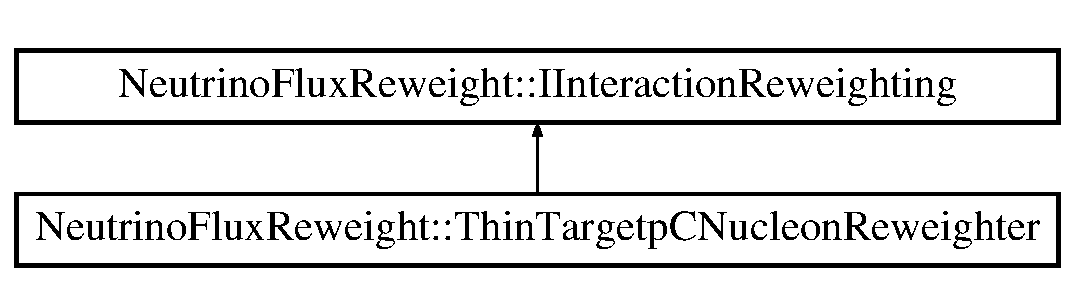
\includegraphics[height=2.000000cm]{class_neutrino_flux_reweight_1_1_thin_targetp_c_nucleon_reweighter}
\end{center}
\end{figure}
\subsection*{Public Member Functions}
\begin{DoxyCompactItemize}
\item 
\hyperlink{class_neutrino_flux_reweight_1_1_thin_targetp_c_nucleon_reweighter_ae60f31bc3ac4ad48e5a32c2b64513457}{Thin\-Targetp\-C\-Nucleon\-Reweighter} (int iuniv, const \hyperlink{class_neutrino_flux_reweight_1_1_parameter_table}{Parameter\-Table} \&cv\-\_\-pars, const \hyperlink{class_neutrino_flux_reweight_1_1_parameter_table}{Parameter\-Table} \&univ\-\_\-pars)
\item 
virtual \hyperlink{class_neutrino_flux_reweight_1_1_thin_targetp_c_nucleon_reweighter_a3d6a84d222e16608b80eaaa11f9be224}{$\sim$\-Thin\-Targetp\-C\-Nucleon\-Reweighter} ()
\item 
virtual bool \hyperlink{class_neutrino_flux_reweight_1_1_thin_targetp_c_nucleon_reweighter_a974bafd329ce322beef237061f446694}{can\-Reweight} (const \hyperlink{class_neutrino_flux_reweight_1_1_interaction_data}{Interaction\-Data} \&aa)
\begin{DoxyCompactList}\small\item\em can the particular instance of this class reweight this interaction? \end{DoxyCompactList}\item 
virtual double \hyperlink{class_neutrino_flux_reweight_1_1_thin_targetp_c_nucleon_reweighter_a6bf9833d98dab84af820f05cf2ff851b}{calculate\-Weight} (const \hyperlink{class_neutrino_flux_reweight_1_1_interaction_data}{Interaction\-Data} \&aa)
\begin{DoxyCompactList}\small\item\em calculate a weight for this interaction given the central value parameters and the parameters for this universe. The weight is something like\-: f(cv)/f(M\-C) $\ast$ f(univ)/f(cv) where cv in this case corresponds to the best value of the parameter, given the data. If univ\-\_\-pars=cv\-\_\-pars then we are calculating a central value weight \end{DoxyCompactList}\item 
double \hyperlink{class_neutrino_flux_reweight_1_1_thin_targetp_c_nucleon_reweighter_a639fe43b3b14e2f1fd277dbbab71cae1}{calculate\-Data\-Scale} (int inc\-\_\-pdg, double inc\-\_\-mom, int prod\-\_\-pdg, double xf, double pt)
\end{DoxyCompactItemize}
\subsection*{Public Attributes}
\begin{DoxyCompactItemize}
\item 
double \hyperlink{class_neutrino_flux_reweight_1_1_thin_targetp_c_nucleon_reweighter_a42193d9c122fad580b96311a7b5e13fb}{data\-\_\-prod\-\_\-xs}
\item 
std\-::vector$<$ float $>$ \hyperlink{class_neutrino_flux_reweight_1_1_thin_targetp_c_nucleon_reweighter_affc490a2bc6f148c1eab12f3cba2457d}{vbin\-\_\-data\-\_\-p}
\item 
std\-::vector$<$ float $>$ \hyperlink{class_neutrino_flux_reweight_1_1_thin_targetp_c_nucleon_reweighter_a3ad5552b4cf05ff2f81a93f3d13432ad}{vbin\-\_\-data\-\_\-n}
\end{DoxyCompactItemize}
\subsection*{Private Attributes}
\begin{DoxyCompactItemize}
\item 
int \hyperlink{class_neutrino_flux_reweight_1_1_thin_targetp_c_nucleon_reweighter_a1c83cab529f6ce4d0f49370289bdf7f9}{i\-Univ}
\item 
const \hyperlink{class_neutrino_flux_reweight_1_1_parameter_table}{Parameter\-Table} \& \hyperlink{class_neutrino_flux_reweight_1_1_thin_targetp_c_nucleon_reweighter_ae86a08603fb33286d960ec7c87024f37}{cv\-Pars}
\item 
const \hyperlink{class_neutrino_flux_reweight_1_1_parameter_table}{Parameter\-Table} \& \hyperlink{class_neutrino_flux_reweight_1_1_thin_targetp_c_nucleon_reweighter_a46e36f7b2a8a95bd45bb748408e3bace}{univ\-Pars}
\end{DoxyCompactItemize}


\subsection{Detailed Description}
Reweighter of thin target p,n production. 

Definition at line 15 of file Thin\-Targetp\-C\-Nucleon\-Reweighter.\-h.



\subsection{Constructor \& Destructor Documentation}
\hypertarget{class_neutrino_flux_reweight_1_1_thin_targetp_c_nucleon_reweighter_ae60f31bc3ac4ad48e5a32c2b64513457}{\index{Neutrino\-Flux\-Reweight\-::\-Thin\-Targetp\-C\-Nucleon\-Reweighter@{Neutrino\-Flux\-Reweight\-::\-Thin\-Targetp\-C\-Nucleon\-Reweighter}!Thin\-Targetp\-C\-Nucleon\-Reweighter@{Thin\-Targetp\-C\-Nucleon\-Reweighter}}
\index{Thin\-Targetp\-C\-Nucleon\-Reweighter@{Thin\-Targetp\-C\-Nucleon\-Reweighter}!NeutrinoFluxReweight::ThinTargetpCNucleonReweighter@{Neutrino\-Flux\-Reweight\-::\-Thin\-Targetp\-C\-Nucleon\-Reweighter}}
\subsubsection[{Thin\-Targetp\-C\-Nucleon\-Reweighter}]{\setlength{\rightskip}{0pt plus 5cm}Neutrino\-Flux\-Reweight\-::\-Thin\-Targetp\-C\-Nucleon\-Reweighter\-::\-Thin\-Targetp\-C\-Nucleon\-Reweighter (
\begin{DoxyParamCaption}
\item[{int}]{iuniv, }
\item[{const {\bf Parameter\-Table} \&}]{cv\-\_\-pars, }
\item[{const {\bf Parameter\-Table} \&}]{univ\-\_\-pars}
\end{DoxyParamCaption}
)}}\label{class_neutrino_flux_reweight_1_1_thin_targetp_c_nucleon_reweighter_ae60f31bc3ac4ad48e5a32c2b64513457}


Definition at line 10 of file Thin\-Targetp\-C\-Nucleon\-Reweighter.\-cpp.


\begin{DoxyCode}
10                                                                                                            
                                  :\hyperlink{class_neutrino_flux_reweight_1_1_thin_targetp_c_nucleon_reweighter_a1c83cab529f6ce4d0f49370289bdf7f9}{iUniv}(iuniv),\hyperlink{class_neutrino_flux_reweight_1_1_thin_targetp_c_nucleon_reweighter_ae86a08603fb33286d960ec7c87024f37}{cvPars}(cv\_pars),\hyperlink{class_neutrino_flux_reweight_1_1_thin_targetp_c_nucleon_reweighter_a46e36f7b2a8a95bd45bb748408e3bace}{univPars}(univ\_pars)\{
11     
12     ThinTargetBins* Thinbins =  \hyperlink{class_neutrino_flux_reweight_1_1_thin_target_bins_aeff5cf7220dd08322f5abac2cbc7ff33}{ThinTargetBins::getInstance}();
13     
14     \hyperlink{class_neutrino_flux_reweight_1_1_thin_targetp_c_nucleon_reweighter_affc490a2bc6f148c1eab12f3cba2457d}{vbin\_data\_p}.reserve(Thinbins->GetNbins\_pC\_pX\_NA49());
15     \hyperlink{class_neutrino_flux_reweight_1_1_thin_targetp_c_nucleon_reweighter_a3ad5552b4cf05ff2f81a93f3d13432ad}{vbin\_data\_n}.reserve(Thinbins->GetNbins\_pC\_nX\_NA49());
16     \textcolor{comment}{// const boost::interprocess::flat\_map<std::string, double>& cv\_table   = cvPars.getMap();}
17     \textcolor{comment}{// const boost::interprocess::flat\_map<std::string, double>& univ\_table = univPars.getMap();}
18     
19      \hyperlink{class_neutrino_flux_reweight_1_1_thin_targetp_c_nucleon_reweighter_a42193d9c122fad580b96311a7b5e13fb}{data\_prod\_xs} = \hyperlink{class_neutrino_flux_reweight_1_1_thin_targetp_c_nucleon_reweighter_a46e36f7b2a8a95bd45bb748408e3bace}{univPars}.\hyperlink{class_neutrino_flux_reweight_1_1_parameter_table_acb7dc8335b65b116f6092f2fa57ca5ed}{getParameterValue}(\textcolor{stringliteral}{"prod\_prtC\_xsec"});
20     
21     \textcolor{comment}{//the number of bins needs to be written from the xmls files }
22     \textcolor{keywordtype}{char} namepar[100];
23     \textcolor{keywordflow}{for}(\textcolor{keywordtype}{int} ii=0;ii<Thinbins->GetNbins\_pC\_pX\_NA49();ii++)\{
24       
25       sprintf(namepar,\textcolor{stringliteral}{"ThinTarget\_pC\_%s\_sys\_%d"},\textcolor{stringliteral}{"p"},ii);
26       \textcolor{keywordtype}{double} data\_cv  = \hyperlink{class_neutrino_flux_reweight_1_1_thin_targetp_c_nucleon_reweighter_ae86a08603fb33286d960ec7c87024f37}{cvPars}.\hyperlink{class_neutrino_flux_reweight_1_1_parameter_table_acb7dc8335b65b116f6092f2fa57ca5ed}{getParameterValue}(std::string(namepar));
27       \textcolor{keywordtype}{double} data\_sys = \hyperlink{class_neutrino_flux_reweight_1_1_thin_targetp_c_nucleon_reweighter_a46e36f7b2a8a95bd45bb748408e3bace}{univPars}.\hyperlink{class_neutrino_flux_reweight_1_1_parameter_table_acb7dc8335b65b116f6092f2fa57ca5ed}{getParameterValue}(std::string(namepar));
28       sprintf(namepar,\textcolor{stringliteral}{"ThinTarget\_pC\_%s\_stats\_%d"},\textcolor{stringliteral}{"p"},ii);
29       \textcolor{keywordtype}{double} data\_sta = \hyperlink{class_neutrino_flux_reweight_1_1_thin_targetp_c_nucleon_reweighter_a46e36f7b2a8a95bd45bb748408e3bace}{univPars}.\hyperlink{class_neutrino_flux_reweight_1_1_parameter_table_acb7dc8335b65b116f6092f2fa57ca5ed}{getParameterValue}(std::string(namepar));       
30       \hyperlink{class_neutrino_flux_reweight_1_1_thin_targetp_c_nucleon_reweighter_affc490a2bc6f148c1eab12f3cba2457d}{vbin\_data\_p}.push\_back(data\_sta + data\_sys - data\_cv);
31       
32     \}    
33 
34     \textcolor{keywordflow}{for}(\textcolor{keywordtype}{int} ii=0;ii<Thinbins->GetNbins\_pC\_nX\_NA49();ii++)\{
35       
36       sprintf(namepar,\textcolor{stringliteral}{"ThinTarget\_pC\_%s\_sys\_%d"},\textcolor{stringliteral}{"n"},ii);
37       \textcolor{keywordtype}{double} data\_cv  = \hyperlink{class_neutrino_flux_reweight_1_1_thin_targetp_c_nucleon_reweighter_ae86a08603fb33286d960ec7c87024f37}{cvPars}.\hyperlink{class_neutrino_flux_reweight_1_1_parameter_table_acb7dc8335b65b116f6092f2fa57ca5ed}{getParameterValue}(std::string(namepar));
38       \textcolor{keywordtype}{double} data\_sys = \hyperlink{class_neutrino_flux_reweight_1_1_thin_targetp_c_nucleon_reweighter_a46e36f7b2a8a95bd45bb748408e3bace}{univPars}.\hyperlink{class_neutrino_flux_reweight_1_1_parameter_table_acb7dc8335b65b116f6092f2fa57ca5ed}{getParameterValue}(std::string(namepar));
39       sprintf(namepar,\textcolor{stringliteral}{"ThinTarget\_pC\_%s\_stats\_%d"},\textcolor{stringliteral}{"n"},ii);
40       \textcolor{keywordtype}{double} data\_sta = \hyperlink{class_neutrino_flux_reweight_1_1_thin_targetp_c_nucleon_reweighter_a46e36f7b2a8a95bd45bb748408e3bace}{univPars}.\hyperlink{class_neutrino_flux_reweight_1_1_parameter_table_acb7dc8335b65b116f6092f2fa57ca5ed}{getParameterValue}(std::string(namepar));       
41       \hyperlink{class_neutrino_flux_reweight_1_1_thin_targetp_c_nucleon_reweighter_a3ad5552b4cf05ff2f81a93f3d13432ad}{vbin\_data\_n}.push\_back(data\_sta + data\_sys - data\_cv);
42       
43     \}   
44 
45     
46   \}
\end{DoxyCode}
\hypertarget{class_neutrino_flux_reweight_1_1_thin_targetp_c_nucleon_reweighter_a3d6a84d222e16608b80eaaa11f9be224}{\index{Neutrino\-Flux\-Reweight\-::\-Thin\-Targetp\-C\-Nucleon\-Reweighter@{Neutrino\-Flux\-Reweight\-::\-Thin\-Targetp\-C\-Nucleon\-Reweighter}!$\sim$\-Thin\-Targetp\-C\-Nucleon\-Reweighter@{$\sim$\-Thin\-Targetp\-C\-Nucleon\-Reweighter}}
\index{$\sim$\-Thin\-Targetp\-C\-Nucleon\-Reweighter@{$\sim$\-Thin\-Targetp\-C\-Nucleon\-Reweighter}!NeutrinoFluxReweight::ThinTargetpCNucleonReweighter@{Neutrino\-Flux\-Reweight\-::\-Thin\-Targetp\-C\-Nucleon\-Reweighter}}
\subsubsection[{$\sim$\-Thin\-Targetp\-C\-Nucleon\-Reweighter}]{\setlength{\rightskip}{0pt plus 5cm}Neutrino\-Flux\-Reweight\-::\-Thin\-Targetp\-C\-Nucleon\-Reweighter\-::$\sim$\-Thin\-Targetp\-C\-Nucleon\-Reweighter (
\begin{DoxyParamCaption}
{}
\end{DoxyParamCaption}
)\hspace{0.3cm}{\ttfamily [virtual]}}}\label{class_neutrino_flux_reweight_1_1_thin_targetp_c_nucleon_reweighter_a3d6a84d222e16608b80eaaa11f9be224}


Definition at line 48 of file Thin\-Targetp\-C\-Nucleon\-Reweighter.\-cpp.


\begin{DoxyCode}
48                                                                 \{
49     
50   \}
\end{DoxyCode}


\subsection{Member Function Documentation}
\hypertarget{class_neutrino_flux_reweight_1_1_thin_targetp_c_nucleon_reweighter_a639fe43b3b14e2f1fd277dbbab71cae1}{\index{Neutrino\-Flux\-Reweight\-::\-Thin\-Targetp\-C\-Nucleon\-Reweighter@{Neutrino\-Flux\-Reweight\-::\-Thin\-Targetp\-C\-Nucleon\-Reweighter}!calculate\-Data\-Scale@{calculate\-Data\-Scale}}
\index{calculate\-Data\-Scale@{calculate\-Data\-Scale}!NeutrinoFluxReweight::ThinTargetpCNucleonReweighter@{Neutrino\-Flux\-Reweight\-::\-Thin\-Targetp\-C\-Nucleon\-Reweighter}}
\subsubsection[{calculate\-Data\-Scale}]{\setlength{\rightskip}{0pt plus 5cm}double Neutrino\-Flux\-Reweight\-::\-Thin\-Targetp\-C\-Nucleon\-Reweighter\-::calculate\-Data\-Scale (
\begin{DoxyParamCaption}
\item[{int}]{inc\-\_\-pdg, }
\item[{double}]{inc\-\_\-mom, }
\item[{int}]{prod\-\_\-pdg, }
\item[{double}]{xf, }
\item[{double}]{pt}
\end{DoxyParamCaption}
)}}\label{class_neutrino_flux_reweight_1_1_thin_targetp_c_nucleon_reweighter_a639fe43b3b14e2f1fd277dbbab71cae1}


Definition at line 119 of file Thin\-Targetp\-C\-Nucleon\-Reweighter.\-cpp.


\begin{DoxyCode}
119                                                                                                            
                   \{
120  
121     \textcolor{keywordtype}{double} scaling\_violation = 1.0;
122     ThinTargetMC*  dtH =  \hyperlink{class_neutrino_flux_reweight_1_1_thin_target_m_c_a2a114747fed2677cd3b7213555c002b9}{ThinTargetMC::getInstance}();
123     \textcolor{comment}{//temporary:}
124     \textcolor{keyword}{const} \textcolor{keywordtype}{int} Nscl = 11;
125     \textcolor{keyword}{const} \textcolor{keywordtype}{int} moms[Nscl] = \{12,20,31,40,50,60,70,80,100,120,158\};
126     
127     \textcolor{keywordtype}{int} idx\_part = -1;
128     \textcolor{keywordflow}{if}(prod\_pdg == 2212)idx\_part = 4;
129     \textcolor{keywordflow}{else} \textcolor{keywordflow}{if}(prod\_pdg == 2112)idx\_part = 5;
130     \textcolor{keywordflow}{else}\{
131       std::cout<<\textcolor{stringliteral}{"Error in the prod particle"}<<std::endl;
132       \textcolor{keywordflow}{return} 1.0;
133     \}
134     
135     \textcolor{keywordtype}{int} idx\_lowp = -1;
136     \textcolor{keywordtype}{int} idx\_hip  = -1;
137     \textcolor{keywordflow}{for}(\textcolor{keywordtype}{int} i=0;i<Nscl-1;i++)\{
138       \textcolor{keywordflow}{if}(inc\_mom>=\textcolor{keywordtype}{double}(moms[i]) && inc\_mom<\textcolor{keywordtype}{double}(moms[i+1]))\{
139         idx\_lowp=i;
140         idx\_hip =i+1;
141       \}
142     \}
143     \textcolor{keywordflow}{if}(idx\_lowp<0 || idx\_hip<0)\{
144       std::cout<<\textcolor{stringliteral}{"Error calculating the scaling"}<<std::endl;
145       \textcolor{keywordflow}{return} 1.0;
146     \}
147 
148     \textcolor{keywordtype}{double} scl\_ref158 = -1.0;
149     \textcolor{keywordtype}{double} scl\_m      =  0.0;
150 
151     \textcolor{keywordflow}{if}(idx\_part==4)\{
152       \textcolor{keywordtype}{int} binid = dtH->hTTScl[idx\_part][Nscl-1]->FindBin(xf,pt);
153       scl\_ref158 = dtH->hTTScl[idx\_part][Nscl-1]->GetBinContent(binid);    
154       \textcolor{comment}{//just provisional... the scaling just reach up to xF=0.8975... consering a close xf value}
155       \textcolor{keywordflow}{if}(xf>0.8975)\{
156         binid = dtH->hTTScl[idx\_part][Nscl-1]->FindBin(0.89,pt);
157         scl\_ref158 = dtH->hTTScl[idx\_part][Nscl-1]->GetBinContent(binid); 
158       \}
159       \textcolor{keywordtype}{double} scl\_low = dtH->hTTScl[idx\_part][idx\_lowp]->GetBinContent(binid);
160       \textcolor{keywordtype}{double} scl\_hi  = dtH->hTTScl[idx\_part][idx\_hip]->GetBinContent(binid);
161       scl\_m   =  scl\_low + (inc\_mom-double(moms[idx\_lowp]))*(scl\_hi-scl\_low)/(double(moms[idx\_hip])-double(
      moms[idx\_lowp]));
162     \}
163     \textcolor{keywordflow}{else} \textcolor{keywordflow}{if}(idx\_part==5)\{
164       \textcolor{keywordtype}{int} binid = dtH->hTTScl\_n[Nscl-1]->FindBin(xf);
165       scl\_ref158 = (double)dtH->hTTScl\_n[Nscl-1]->GetBinContent(binid); 
166       \textcolor{keywordtype}{double} scl\_low = dtH->hTTScl\_n[idx\_lowp]->GetBinContent(binid);
167       \textcolor{keywordtype}{double} scl\_hi  = dtH->hTTScl\_n[idx\_hip]->GetBinContent(binid);
168       scl\_m   =  scl\_low + (inc\_mom-double(moms[idx\_lowp]))*(scl\_hi-scl\_low)/(double(moms[idx\_hip])-double(
      moms[idx\_lowp]));
169     \}
170     \textcolor{keywordflow}{else}\{
171       std::cout<<\textcolor{stringliteral}{"still error, not expected here!!"}<<std::endl;
172       \textcolor{keywordflow}{return} 1.0;
173     \}
174     
175     \textcolor{keywordflow}{if}(scl\_ref158 < 1.e-10 || scl\_m<1.e-10)\{
176       std::cout<<\textcolor{stringliteral}{"scale problems: "}<<scl\_ref158<<\textcolor{stringliteral}{" "}<<scl\_m<<\textcolor{stringliteral}{" "}<<inc\_pdg<<\textcolor{stringliteral}{" "}<<inc\_mom<<\textcolor{stringliteral}{" "}<<prod\_pdg<<\textcolor{stringliteral}{" "}
      <<xf<<\textcolor{stringliteral}{" "}<<pt<<std::endl;
177       \textcolor{keywordflow}{return} 1.0;
178     \}   
179     scaling\_violation = scl\_m/scl\_ref158;
180     \textcolor{keywordflow}{return} scaling\_violation;
181   \}
\end{DoxyCode}
\hypertarget{class_neutrino_flux_reweight_1_1_thin_targetp_c_nucleon_reweighter_a6bf9833d98dab84af820f05cf2ff851b}{\index{Neutrino\-Flux\-Reweight\-::\-Thin\-Targetp\-C\-Nucleon\-Reweighter@{Neutrino\-Flux\-Reweight\-::\-Thin\-Targetp\-C\-Nucleon\-Reweighter}!calculate\-Weight@{calculate\-Weight}}
\index{calculate\-Weight@{calculate\-Weight}!NeutrinoFluxReweight::ThinTargetpCNucleonReweighter@{Neutrino\-Flux\-Reweight\-::\-Thin\-Targetp\-C\-Nucleon\-Reweighter}}
\subsubsection[{calculate\-Weight}]{\setlength{\rightskip}{0pt plus 5cm}double Neutrino\-Flux\-Reweight\-::\-Thin\-Targetp\-C\-Nucleon\-Reweighter\-::calculate\-Weight (
\begin{DoxyParamCaption}
\item[{const {\bf Interaction\-Data} \&}]{inter\-\_\-data}
\end{DoxyParamCaption}
)\hspace{0.3cm}{\ttfamily [virtual]}}}\label{class_neutrino_flux_reweight_1_1_thin_targetp_c_nucleon_reweighter_a6bf9833d98dab84af820f05cf2ff851b}


calculate a weight for this interaction given the central value parameters and the parameters for this universe. The weight is something like\-: f(cv)/f(M\-C) $\ast$ f(univ)/f(cv) where cv in this case corresponds to the best value of the parameter, given the data. If univ\-\_\-pars=cv\-\_\-pars then we are calculating a central value weight 



Implements \hyperlink{class_neutrino_flux_reweight_1_1_i_interaction_reweighting_a49b0d73e778411d629205d23575703c3}{Neutrino\-Flux\-Reweight\-::\-I\-Interaction\-Reweighting}.



Definition at line 74 of file Thin\-Targetp\-C\-Nucleon\-Reweighter.\-cpp.


\begin{DoxyCode}
74                                                                                 \{
75  
76     \textcolor{comment}{//quick check:}
77     \textcolor{keywordtype}{double} wgt = 1.0;
78     ThinTargetBins*  Thinbins =  \hyperlink{class_neutrino_flux_reweight_1_1_thin_target_bins_aeff5cf7220dd08322f5abac2cbc7ff33}{ThinTargetBins::getInstance}();
79     \textcolor{keywordtype}{int} bin\_p = Thinbins->BinID\_pC\_p(aa.xF,aa.Pt,aa.Prod\_pdg);
80     \textcolor{keywordtype}{int} bin\_n = Thinbins->BinID\_pC\_n(aa.xF,aa.Prod\_pdg);
81     \textcolor{keywordflow}{if}(bin\_p < 0 && bin\_n < 0)\{
82       \textcolor{comment}{//std::cout<<"Not bin found "<<std::endl;}
83       \textcolor{keywordflow}{return} wgt;
84     \}
85 
86     \textcolor{comment}{//Calculating the scale:}
87     \textcolor{keywordtype}{double} data\_scale = \hyperlink{class_neutrino_flux_reweight_1_1_thin_targetp_c_nucleon_reweighter_a639fe43b3b14e2f1fd277dbbab71cae1}{calculateDataScale}(aa.Inc\_pdg,aa.Inc\_P,aa.Prod\_pdg,aa.xF,aa.Pt);
88     \textcolor{keywordtype}{double} dataval = -1;
89     \textcolor{keywordflow}{if}(aa.Prod\_pdg==2212)dataval = \hyperlink{class_neutrino_flux_reweight_1_1_thin_targetp_c_nucleon_reweighter_affc490a2bc6f148c1eab12f3cba2457d}{vbin\_data\_p}[bin\_p];
90     \textcolor{keywordflow}{if}(aa.Prod\_pdg==2112)dataval = \hyperlink{class_neutrino_flux_reweight_1_1_thin_targetp_c_nucleon_reweighter_a3ad5552b4cf05ff2f81a93f3d13432ad}{vbin\_data\_n}[bin\_n];
91     
92     \textcolor{keywordflow}{if}(dataval<1.e-12)\{
93       \textcolor{comment}{//std::cout<<"Not data found "<<std::endl;}
94       \textcolor{keywordflow}{return} wgt;
95     \}
96 
97     \textcolor{comment}{//checking if this is the first interaction:}
98     \textcolor{keywordflow}{if}(aa.gen==0 && aa.Prod\_pdg==2212)dataval /= \hyperlink{class_neutrino_flux_reweight_1_1_thin_targetp_c_nucleon_reweighter_a42193d9c122fad580b96311a7b5e13fb}{data\_prod\_xs};
99     \textcolor{keywordflow}{if}(aa.gen>0  && aa.Prod\_pdg==2212)dataval /= 1.0;
100     \textcolor{keywordflow}{if}(aa.gen==0 && aa.Prod\_pdg==2112)dataval /= 1.0;
101     \textcolor{keywordflow}{if}(aa.gen>0  && aa.Prod\_pdg==2112)dataval *= \hyperlink{class_neutrino_flux_reweight_1_1_thin_targetp_c_nucleon_reweighter_a42193d9c122fad580b96311a7b5e13fb}{data\_prod\_xs};
102     
103     dataval *= data\_scale;
104  
105     ThinTargetMC*  mc =  \hyperlink{class_neutrino_flux_reweight_1_1_thin_target_m_c_a2a114747fed2677cd3b7213555c002b9}{ThinTargetMC::getInstance}(); 
106     \textcolor{keywordtype}{double} mc\_cv = mc->getMCval\_pC\_X(aa.Inc\_P,aa.xF,aa.Pt,aa.Prod\_pdg); 
107     \textcolor{keywordtype}{double} mc\_prod = mc->getMCxs\_pC\_nucleon(aa.gen,aa.Prod\_pdg,aa.Inc\_P);    
108     mc\_cv /= mc\_prod;
109     \textcolor{keywordflow}{if}(mc\_cv<1.e-12)\textcolor{keywordflow}{return} wgt;
110     wgt = dataval/mc\_cv;
111     \textcolor{keywordflow}{if}(wgt<0)\{
112       std::cout<<\textcolor{stringliteral}{"TTPCNU check wgt(<0) "}<<\hyperlink{class_neutrino_flux_reweight_1_1_thin_targetp_c_nucleon_reweighter_a1c83cab529f6ce4d0f49370289bdf7f9}{iUniv}<<\textcolor{stringliteral}{" "}<<wgt<<\textcolor{stringliteral}{" "}<<aa.Inc\_P<<\textcolor{stringliteral}{" "}<<aa.xF<<\textcolor{stringliteral}{" "}<<aa.Pt<<\textcolor{stringliteral}{" "}<
      <aa.Prod\_pdg<<\textcolor{stringliteral}{" "}<<(mc->getMCxs\_pC\_nucleon(aa.gen,aa.Prod\_pdg,aa.Inc\_P))<<std::endl;
113       \textcolor{keywordflow}{return} 1.0;
114     \}
115 
116     \textcolor{keywordflow}{return} wgt;
117   \}
\end{DoxyCode}
\hypertarget{class_neutrino_flux_reweight_1_1_thin_targetp_c_nucleon_reweighter_a974bafd329ce322beef237061f446694}{\index{Neutrino\-Flux\-Reweight\-::\-Thin\-Targetp\-C\-Nucleon\-Reweighter@{Neutrino\-Flux\-Reweight\-::\-Thin\-Targetp\-C\-Nucleon\-Reweighter}!can\-Reweight@{can\-Reweight}}
\index{can\-Reweight@{can\-Reweight}!NeutrinoFluxReweight::ThinTargetpCNucleonReweighter@{Neutrino\-Flux\-Reweight\-::\-Thin\-Targetp\-C\-Nucleon\-Reweighter}}
\subsubsection[{can\-Reweight}]{\setlength{\rightskip}{0pt plus 5cm}bool Neutrino\-Flux\-Reweight\-::\-Thin\-Targetp\-C\-Nucleon\-Reweighter\-::can\-Reweight (
\begin{DoxyParamCaption}
\item[{const {\bf Interaction\-Data} \&}]{aa}
\end{DoxyParamCaption}
)\hspace{0.3cm}{\ttfamily [virtual]}}}\label{class_neutrino_flux_reweight_1_1_thin_targetp_c_nucleon_reweighter_a974bafd329ce322beef237061f446694}


can the particular instance of this class reweight this interaction? 



Implements \hyperlink{class_neutrino_flux_reweight_1_1_i_interaction_reweighting_aa3d1d3f37a93b02e447cf5eca333ac8d}{Neutrino\-Flux\-Reweight\-::\-I\-Interaction\-Reweighting}.



Definition at line 51 of file Thin\-Targetp\-C\-Nucleon\-Reweighter.\-cpp.


\begin{DoxyCode}
51                                                                           \{
52 
53     \textcolor{comment}{//checking:}
54     std::string mode(getenv(\textcolor{stringliteral}{"MODE"}));
55     \textcolor{keywordflow}{if}(aa.Inc\_pdg != 2212)\textcolor{keywordflow}{return} \textcolor{keyword}{false};
56     \textcolor{keywordflow}{if}(aa.Inc\_P < 12.0)\textcolor{keywordflow}{return} \textcolor{keyword}{false};
57     \textcolor{comment}{//volume check: }
58     \textcolor{keywordtype}{bool} is\_wrong\_volume = aa.Vol != \textcolor{stringliteral}{"TGT1"} && aa.Vol != \textcolor{stringliteral}{"BudalMonitor"} && aa.Vol != \textcolor{stringliteral}{"Budal\_HFVS"} && aa.Vol
       != \textcolor{stringliteral}{"Budal\_VFHS"};
59     \textcolor{keywordflow}{if}( (mode==\textcolor{stringliteral}{"REF"}) || (mode==\textcolor{stringliteral}{"OPT"}) )\{
60       is\_wrong\_volume = aa.Vol != \textcolor{stringliteral}{"TargetFinHorizontal"} && aa.Vol != \textcolor{stringliteral}{"TargetNoSplitSegment"} && aa.Vol!=\textcolor{stringliteral}{"
      tCoreLog"};
61     \}
62     \textcolor{keywordflow}{if}(is\_wrong\_volume)\textcolor{keywordflow}{return} \textcolor{keyword}{false};
63     \textcolor{comment}{//}
64     \textcolor{keywordflow}{if}(aa.Prod\_pdg != 2212 && aa.Prod\_pdg != 2112)\textcolor{keywordflow}{return} \textcolor{keyword}{false};
65     
66     ThinTargetBins*  Thinbins =  \hyperlink{class_neutrino_flux_reweight_1_1_thin_target_bins_aeff5cf7220dd08322f5abac2cbc7ff33}{ThinTargetBins::getInstance}();
67     \textcolor{keywordtype}{int} bin\_p      = Thinbins->BinID\_pC\_p(aa.xF,aa.Pt,aa.Prod\_pdg);
68     \textcolor{keywordtype}{int} bin\_n      = Thinbins->BinID\_pC\_n(aa.xF,aa.Prod\_pdg);
69     \textcolor{keywordflow}{if}(bin\_p < 0 && bin\_n < 0)\textcolor{keywordflow}{return} \textcolor{keyword}{false};
70     \textcolor{keywordflow}{else} \textcolor{keywordflow}{return} \textcolor{keyword}{true};
71     
72   \}
\end{DoxyCode}


\subsection{Member Data Documentation}
\hypertarget{class_neutrino_flux_reweight_1_1_thin_targetp_c_nucleon_reweighter_ae86a08603fb33286d960ec7c87024f37}{\index{Neutrino\-Flux\-Reweight\-::\-Thin\-Targetp\-C\-Nucleon\-Reweighter@{Neutrino\-Flux\-Reweight\-::\-Thin\-Targetp\-C\-Nucleon\-Reweighter}!cv\-Pars@{cv\-Pars}}
\index{cv\-Pars@{cv\-Pars}!NeutrinoFluxReweight::ThinTargetpCNucleonReweighter@{Neutrino\-Flux\-Reweight\-::\-Thin\-Targetp\-C\-Nucleon\-Reweighter}}
\subsubsection[{cv\-Pars}]{\setlength{\rightskip}{0pt plus 5cm}const {\bf Parameter\-Table}\& Neutrino\-Flux\-Reweight\-::\-Thin\-Targetp\-C\-Nucleon\-Reweighter\-::cv\-Pars\hspace{0.3cm}{\ttfamily [private]}}}\label{class_neutrino_flux_reweight_1_1_thin_targetp_c_nucleon_reweighter_ae86a08603fb33286d960ec7c87024f37}


Definition at line 29 of file Thin\-Targetp\-C\-Nucleon\-Reweighter.\-h.

\hypertarget{class_neutrino_flux_reweight_1_1_thin_targetp_c_nucleon_reweighter_a42193d9c122fad580b96311a7b5e13fb}{\index{Neutrino\-Flux\-Reweight\-::\-Thin\-Targetp\-C\-Nucleon\-Reweighter@{Neutrino\-Flux\-Reweight\-::\-Thin\-Targetp\-C\-Nucleon\-Reweighter}!data\-\_\-prod\-\_\-xs@{data\-\_\-prod\-\_\-xs}}
\index{data\-\_\-prod\-\_\-xs@{data\-\_\-prod\-\_\-xs}!NeutrinoFluxReweight::ThinTargetpCNucleonReweighter@{Neutrino\-Flux\-Reweight\-::\-Thin\-Targetp\-C\-Nucleon\-Reweighter}}
\subsubsection[{data\-\_\-prod\-\_\-xs}]{\setlength{\rightskip}{0pt plus 5cm}double Neutrino\-Flux\-Reweight\-::\-Thin\-Targetp\-C\-Nucleon\-Reweighter\-::data\-\_\-prod\-\_\-xs}}\label{class_neutrino_flux_reweight_1_1_thin_targetp_c_nucleon_reweighter_a42193d9c122fad580b96311a7b5e13fb}


Definition at line 24 of file Thin\-Targetp\-C\-Nucleon\-Reweighter.\-h.

\hypertarget{class_neutrino_flux_reweight_1_1_thin_targetp_c_nucleon_reweighter_a1c83cab529f6ce4d0f49370289bdf7f9}{\index{Neutrino\-Flux\-Reweight\-::\-Thin\-Targetp\-C\-Nucleon\-Reweighter@{Neutrino\-Flux\-Reweight\-::\-Thin\-Targetp\-C\-Nucleon\-Reweighter}!i\-Univ@{i\-Univ}}
\index{i\-Univ@{i\-Univ}!NeutrinoFluxReweight::ThinTargetpCNucleonReweighter@{Neutrino\-Flux\-Reweight\-::\-Thin\-Targetp\-C\-Nucleon\-Reweighter}}
\subsubsection[{i\-Univ}]{\setlength{\rightskip}{0pt plus 5cm}int Neutrino\-Flux\-Reweight\-::\-Thin\-Targetp\-C\-Nucleon\-Reweighter\-::i\-Univ\hspace{0.3cm}{\ttfamily [private]}}}\label{class_neutrino_flux_reweight_1_1_thin_targetp_c_nucleon_reweighter_a1c83cab529f6ce4d0f49370289bdf7f9}


Definition at line 28 of file Thin\-Targetp\-C\-Nucleon\-Reweighter.\-h.

\hypertarget{class_neutrino_flux_reweight_1_1_thin_targetp_c_nucleon_reweighter_a46e36f7b2a8a95bd45bb748408e3bace}{\index{Neutrino\-Flux\-Reweight\-::\-Thin\-Targetp\-C\-Nucleon\-Reweighter@{Neutrino\-Flux\-Reweight\-::\-Thin\-Targetp\-C\-Nucleon\-Reweighter}!univ\-Pars@{univ\-Pars}}
\index{univ\-Pars@{univ\-Pars}!NeutrinoFluxReweight::ThinTargetpCNucleonReweighter@{Neutrino\-Flux\-Reweight\-::\-Thin\-Targetp\-C\-Nucleon\-Reweighter}}
\subsubsection[{univ\-Pars}]{\setlength{\rightskip}{0pt plus 5cm}const {\bf Parameter\-Table}\& Neutrino\-Flux\-Reweight\-::\-Thin\-Targetp\-C\-Nucleon\-Reweighter\-::univ\-Pars\hspace{0.3cm}{\ttfamily [private]}}}\label{class_neutrino_flux_reweight_1_1_thin_targetp_c_nucleon_reweighter_a46e36f7b2a8a95bd45bb748408e3bace}


Definition at line 30 of file Thin\-Targetp\-C\-Nucleon\-Reweighter.\-h.

\hypertarget{class_neutrino_flux_reweight_1_1_thin_targetp_c_nucleon_reweighter_a3ad5552b4cf05ff2f81a93f3d13432ad}{\index{Neutrino\-Flux\-Reweight\-::\-Thin\-Targetp\-C\-Nucleon\-Reweighter@{Neutrino\-Flux\-Reweight\-::\-Thin\-Targetp\-C\-Nucleon\-Reweighter}!vbin\-\_\-data\-\_\-n@{vbin\-\_\-data\-\_\-n}}
\index{vbin\-\_\-data\-\_\-n@{vbin\-\_\-data\-\_\-n}!NeutrinoFluxReweight::ThinTargetpCNucleonReweighter@{Neutrino\-Flux\-Reweight\-::\-Thin\-Targetp\-C\-Nucleon\-Reweighter}}
\subsubsection[{vbin\-\_\-data\-\_\-n}]{\setlength{\rightskip}{0pt plus 5cm}std\-::vector$<$float$>$ Neutrino\-Flux\-Reweight\-::\-Thin\-Targetp\-C\-Nucleon\-Reweighter\-::vbin\-\_\-data\-\_\-n}}\label{class_neutrino_flux_reweight_1_1_thin_targetp_c_nucleon_reweighter_a3ad5552b4cf05ff2f81a93f3d13432ad}


Definition at line 25 of file Thin\-Targetp\-C\-Nucleon\-Reweighter.\-h.

\hypertarget{class_neutrino_flux_reweight_1_1_thin_targetp_c_nucleon_reweighter_affc490a2bc6f148c1eab12f3cba2457d}{\index{Neutrino\-Flux\-Reweight\-::\-Thin\-Targetp\-C\-Nucleon\-Reweighter@{Neutrino\-Flux\-Reweight\-::\-Thin\-Targetp\-C\-Nucleon\-Reweighter}!vbin\-\_\-data\-\_\-p@{vbin\-\_\-data\-\_\-p}}
\index{vbin\-\_\-data\-\_\-p@{vbin\-\_\-data\-\_\-p}!NeutrinoFluxReweight::ThinTargetpCNucleonReweighter@{Neutrino\-Flux\-Reweight\-::\-Thin\-Targetp\-C\-Nucleon\-Reweighter}}
\subsubsection[{vbin\-\_\-data\-\_\-p}]{\setlength{\rightskip}{0pt plus 5cm}std\-::vector$<$float$>$ Neutrino\-Flux\-Reweight\-::\-Thin\-Targetp\-C\-Nucleon\-Reweighter\-::vbin\-\_\-data\-\_\-p}}\label{class_neutrino_flux_reweight_1_1_thin_targetp_c_nucleon_reweighter_affc490a2bc6f148c1eab12f3cba2457d}


Definition at line 25 of file Thin\-Targetp\-C\-Nucleon\-Reweighter.\-h.



The documentation for this class was generated from the following files\-:\begin{DoxyCompactItemize}
\item 
include/\hyperlink{_thin_targetp_c_nucleon_reweighter_8h}{Thin\-Targetp\-C\-Nucleon\-Reweighter.\-h}\item 
src/\hyperlink{_thin_targetp_c_nucleon_reweighter_8cpp}{Thin\-Targetp\-C\-Nucleon\-Reweighter.\-cpp}\end{DoxyCompactItemize}

\hypertarget{class_neutrino_flux_reweight_1_1_thin_targetp_c_pion_reweighter}{\section{Neutrino\-Flux\-Reweight\-:\-:Thin\-Targetp\-C\-Pion\-Reweighter Class Reference}
\label{class_neutrino_flux_reweight_1_1_thin_targetp_c_pion_reweighter}\index{Neutrino\-Flux\-Reweight\-::\-Thin\-Targetp\-C\-Pion\-Reweighter@{Neutrino\-Flux\-Reweight\-::\-Thin\-Targetp\-C\-Pion\-Reweighter}}
}


Reweighter of thin target pion production.  




{\ttfamily \#include $<$Thin\-Targetp\-C\-Pion\-Reweighter.\-h$>$}

Inheritance diagram for Neutrino\-Flux\-Reweight\-:\-:Thin\-Targetp\-C\-Pion\-Reweighter\-:\begin{figure}[H]
\begin{center}
\leavevmode
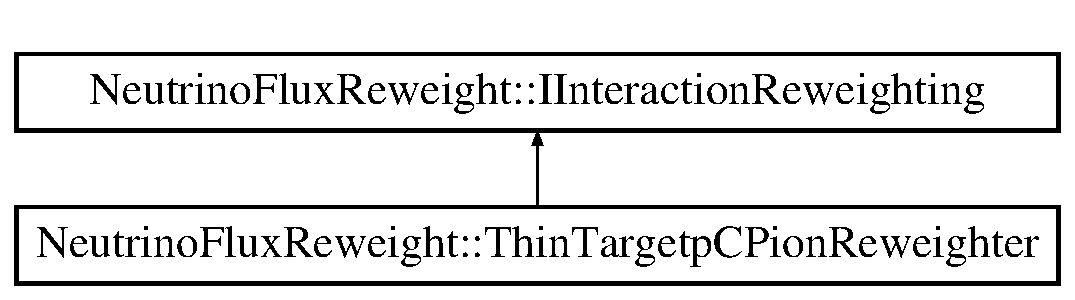
\includegraphics[height=2.000000cm]{class_neutrino_flux_reweight_1_1_thin_targetp_c_pion_reweighter}
\end{center}
\end{figure}
\subsection*{Public Member Functions}
\begin{DoxyCompactItemize}
\item 
\hyperlink{class_neutrino_flux_reweight_1_1_thin_targetp_c_pion_reweighter_a461135f73ed6cea79b71cc37d17466e2}{Thin\-Targetp\-C\-Pion\-Reweighter} (int iuniv, const \hyperlink{class_neutrino_flux_reweight_1_1_parameter_table}{Parameter\-Table} \&cv\-\_\-pars, const \hyperlink{class_neutrino_flux_reweight_1_1_parameter_table}{Parameter\-Table} \&univ\-\_\-pars)
\item 
virtual \hyperlink{class_neutrino_flux_reweight_1_1_thin_targetp_c_pion_reweighter_a0d76e9167d90e1c56a7291ae6d219fd2}{$\sim$\-Thin\-Targetp\-C\-Pion\-Reweighter} ()
\item 
virtual bool \hyperlink{class_neutrino_flux_reweight_1_1_thin_targetp_c_pion_reweighter_a09067dcacb294ca133e2660d61302e85}{can\-Reweight} (const \hyperlink{class_neutrino_flux_reweight_1_1_interaction_data}{Interaction\-Data} \&aa)
\begin{DoxyCompactList}\small\item\em can the particular instance of this class reweight this interaction? \end{DoxyCompactList}\item 
virtual double \hyperlink{class_neutrino_flux_reweight_1_1_thin_targetp_c_pion_reweighter_ab797bbeeedb04cda73feef891434cd5f}{calculate\-Weight} (const \hyperlink{class_neutrino_flux_reweight_1_1_interaction_data}{Interaction\-Data} \&inter\-\_\-data)
\begin{DoxyCompactList}\small\item\em calculate a weight for this interaction given the central value parameters and the parameters for this universe. The weight is something like\-: f(cv)/f(M\-C) $\ast$ f(univ)/f(cv) where cv in this case corresponds to the best value of the parameter, given the data. If univ\-\_\-pars=cv\-\_\-pars then we are calculating a central value weight \end{DoxyCompactList}\item 
double \hyperlink{class_neutrino_flux_reweight_1_1_thin_targetp_c_pion_reweighter_ac34d175572ca9ac093e973e877891eae}{calculate\-Data\-Scale} (int inc\-\_\-pdg, double inc\-\_\-mom, int prod\-\_\-pdg, double xf, double pt)
\end{DoxyCompactItemize}
\subsection*{Public Attributes}
\begin{DoxyCompactItemize}
\item 
double \hyperlink{class_neutrino_flux_reweight_1_1_thin_targetp_c_pion_reweighter_ae2c5b20aa1823516579b0684d188d75d}{data\-\_\-prod\-\_\-xs}
\item 
std\-::vector$<$ float $>$ \hyperlink{class_neutrino_flux_reweight_1_1_thin_targetp_c_pion_reweighter_a3602ae8237c0cc7729045b13b90874b4}{vbin\-\_\-data\-\_\-pip}
\item 
std\-::vector$<$ float $>$ \hyperlink{class_neutrino_flux_reweight_1_1_thin_targetp_c_pion_reweighter_aea0dca1b93e560e26871da0bdf1ac075}{vbin\-\_\-data\-\_\-pim}
\item 
std\-::vector$<$ float $>$ \hyperlink{class_neutrino_flux_reweight_1_1_thin_targetp_c_pion_reweighter_a844e9c7ba521a42ce5ebe5fbb5b2d5f4}{bart\-\_\-vbin\-\_\-data\-\_\-pip}
\item 
std\-::vector$<$ float $>$ \hyperlink{class_neutrino_flux_reweight_1_1_thin_targetp_c_pion_reweighter_a9d7ffcf3ca0c5a7b0f1c37435cc86403}{bart\-\_\-vbin\-\_\-data\-\_\-pim}
\end{DoxyCompactItemize}
\subsection*{Private Attributes}
\begin{DoxyCompactItemize}
\item 
int \hyperlink{class_neutrino_flux_reweight_1_1_thin_targetp_c_pion_reweighter_a59ed15e151960ba8dc990d8c6bbd7567}{i\-Univ}
\item 
const \hyperlink{class_neutrino_flux_reweight_1_1_parameter_table}{Parameter\-Table} \& \hyperlink{class_neutrino_flux_reweight_1_1_thin_targetp_c_pion_reweighter_ad0ab176cd637c51c8ca5d4f87ed93ded}{cv\-Pars}
\item 
const \hyperlink{class_neutrino_flux_reweight_1_1_parameter_table}{Parameter\-Table} \& \hyperlink{class_neutrino_flux_reweight_1_1_thin_targetp_c_pion_reweighter_afc6d553d64c70f7b98636b2bb8a13b43}{univ\-Pars}
\item 
float \hyperlink{class_neutrino_flux_reweight_1_1_thin_targetp_c_pion_reweighter_a87d4a2cfb3ce6e4e5c7f0f3be1144915}{aux\-\_\-par}
\end{DoxyCompactItemize}


\subsection{Detailed Description}
Reweighter of thin target pion production. 

Definition at line 18 of file Thin\-Targetp\-C\-Pion\-Reweighter.\-h.



\subsection{Constructor \& Destructor Documentation}
\hypertarget{class_neutrino_flux_reweight_1_1_thin_targetp_c_pion_reweighter_a461135f73ed6cea79b71cc37d17466e2}{\index{Neutrino\-Flux\-Reweight\-::\-Thin\-Targetp\-C\-Pion\-Reweighter@{Neutrino\-Flux\-Reweight\-::\-Thin\-Targetp\-C\-Pion\-Reweighter}!Thin\-Targetp\-C\-Pion\-Reweighter@{Thin\-Targetp\-C\-Pion\-Reweighter}}
\index{Thin\-Targetp\-C\-Pion\-Reweighter@{Thin\-Targetp\-C\-Pion\-Reweighter}!NeutrinoFluxReweight::ThinTargetpCPionReweighter@{Neutrino\-Flux\-Reweight\-::\-Thin\-Targetp\-C\-Pion\-Reweighter}}
\subsubsection[{Thin\-Targetp\-C\-Pion\-Reweighter}]{\setlength{\rightskip}{0pt plus 5cm}Neutrino\-Flux\-Reweight\-::\-Thin\-Targetp\-C\-Pion\-Reweighter\-::\-Thin\-Targetp\-C\-Pion\-Reweighter (
\begin{DoxyParamCaption}
\item[{int}]{iuniv, }
\item[{const {\bf Parameter\-Table} \&}]{cv\-\_\-pars, }
\item[{const {\bf Parameter\-Table} \&}]{univ\-\_\-pars}
\end{DoxyParamCaption}
)}}\label{class_neutrino_flux_reweight_1_1_thin_targetp_c_pion_reweighter_a461135f73ed6cea79b71cc37d17466e2}


Definition at line 11 of file Thin\-Targetp\-C\-Pion\-Reweighter.\-cpp.


\begin{DoxyCode}
11                                                                                                            
                            :\hyperlink{class_neutrino_flux_reweight_1_1_thin_targetp_c_pion_reweighter_a59ed15e151960ba8dc990d8c6bbd7567}{iUniv}(iuniv),\hyperlink{class_neutrino_flux_reweight_1_1_thin_targetp_c_pion_reweighter_ad0ab176cd637c51c8ca5d4f87ed93ded}{cvPars}(cv\_pars),\hyperlink{class_neutrino_flux_reweight_1_1_thin_targetp_c_pion_reweighter_afc6d553d64c70f7b98636b2bb8a13b43}{univPars}(univ\_pars)\{
12     
13     ThinTargetBins*  Thinbins =  \hyperlink{class_neutrino_flux_reweight_1_1_thin_target_bins_aeff5cf7220dd08322f5abac2cbc7ff33}{ThinTargetBins::getInstance}();
14     \hyperlink{class_neutrino_flux_reweight_1_1_thin_targetp_c_pion_reweighter_a3602ae8237c0cc7729045b13b90874b4}{vbin\_data\_pip}.reserve(Thinbins->GetNbins\_pC\_piX\_NA49());
15     \hyperlink{class_neutrino_flux_reweight_1_1_thin_targetp_c_pion_reweighter_aea0dca1b93e560e26871da0bdf1ac075}{vbin\_data\_pim}.reserve(Thinbins->GetNbins\_pC\_piX\_NA49());
16     \hyperlink{class_neutrino_flux_reweight_1_1_thin_targetp_c_pion_reweighter_a844e9c7ba521a42ce5ebe5fbb5b2d5f4}{bart\_vbin\_data\_pip}.reserve(Thinbins->GetNbins\_pC\_piX\_Barton());
17     \hyperlink{class_neutrino_flux_reweight_1_1_thin_targetp_c_pion_reweighter_a9d7ffcf3ca0c5a7b0f1c37435cc86403}{bart\_vbin\_data\_pim}.reserve(Thinbins->GetNbins\_pC\_piX\_Barton());
18     
19     \textcolor{comment}{// const boost::interprocess::flat\_map<std::string, double>& cv\_table   = cvPars.getMap();}
20     \textcolor{comment}{// const boost::interprocess::flat\_map<std::string, double>& univ\_table = univPars.getMap();}
21     
22     \hyperlink{class_neutrino_flux_reweight_1_1_thin_targetp_c_pion_reweighter_ae2c5b20aa1823516579b0684d188d75d}{data\_prod\_xs} = \hyperlink{class_neutrino_flux_reweight_1_1_thin_targetp_c_pion_reweighter_afc6d553d64c70f7b98636b2bb8a13b43}{univPars}.\hyperlink{class_neutrino_flux_reweight_1_1_parameter_table_acb7dc8335b65b116f6092f2fa57ca5ed}{getParameterValue}(\textcolor{stringliteral}{"prod\_prtC\_xsec"});
23     
24     \textcolor{comment}{//the number of bins needs to be written from the xmls files }
25     \textcolor{keywordtype}{char} namepar[100];
26     \textcolor{keywordflow}{for}(\textcolor{keywordtype}{int} ii=0;ii<Thinbins->GetNbins\_pC\_piX\_NA49();ii++)\{
27       
28       sprintf(namepar,\textcolor{stringliteral}{"ThinTarget\_pC\_%s\_sys\_%d"},\textcolor{stringliteral}{"pip"},ii);
29       \textcolor{keywordtype}{double} data\_cv  = \hyperlink{class_neutrino_flux_reweight_1_1_thin_targetp_c_pion_reweighter_ad0ab176cd637c51c8ca5d4f87ed93ded}{cvPars}.\hyperlink{class_neutrino_flux_reweight_1_1_parameter_table_acb7dc8335b65b116f6092f2fa57ca5ed}{getParameterValue}(std::string(namepar));
30       \textcolor{keywordtype}{double} data\_sys = \hyperlink{class_neutrino_flux_reweight_1_1_thin_targetp_c_pion_reweighter_afc6d553d64c70f7b98636b2bb8a13b43}{univPars}.\hyperlink{class_neutrino_flux_reweight_1_1_parameter_table_acb7dc8335b65b116f6092f2fa57ca5ed}{getParameterValue}(std::string(namepar));
31       sprintf(namepar,\textcolor{stringliteral}{"ThinTarget\_pC\_%s\_stats\_%d"},\textcolor{stringliteral}{"pip"},ii);
32       \textcolor{keywordtype}{double} data\_sta = \hyperlink{class_neutrino_flux_reweight_1_1_thin_targetp_c_pion_reweighter_afc6d553d64c70f7b98636b2bb8a13b43}{univPars}.\hyperlink{class_neutrino_flux_reweight_1_1_parameter_table_acb7dc8335b65b116f6092f2fa57ca5ed}{getParameterValue}(std::string(namepar));       
33       \hyperlink{class_neutrino_flux_reweight_1_1_thin_targetp_c_pion_reweighter_a3602ae8237c0cc7729045b13b90874b4}{vbin\_data\_pip}.push\_back(data\_sta + data\_sys - data\_cv);
34       
35       sprintf(namepar,\textcolor{stringliteral}{"ThinTarget\_pC\_%s\_sys\_%d"},\textcolor{stringliteral}{"pim"},ii);
36       data\_cv  = \hyperlink{class_neutrino_flux_reweight_1_1_thin_targetp_c_pion_reweighter_ad0ab176cd637c51c8ca5d4f87ed93ded}{cvPars}.\hyperlink{class_neutrino_flux_reweight_1_1_parameter_table_acb7dc8335b65b116f6092f2fa57ca5ed}{getParameterValue}(std::string(namepar));
37       data\_sys = \hyperlink{class_neutrino_flux_reweight_1_1_thin_targetp_c_pion_reweighter_afc6d553d64c70f7b98636b2bb8a13b43}{univPars}.\hyperlink{class_neutrino_flux_reweight_1_1_parameter_table_acb7dc8335b65b116f6092f2fa57ca5ed}{getParameterValue}(std::string(namepar));
38       sprintf(namepar,\textcolor{stringliteral}{"ThinTarget\_pC\_%s\_stats\_%d"},\textcolor{stringliteral}{"pim"},ii);
39       data\_sta = \hyperlink{class_neutrino_flux_reweight_1_1_thin_targetp_c_pion_reweighter_afc6d553d64c70f7b98636b2bb8a13b43}{univPars}.\hyperlink{class_neutrino_flux_reweight_1_1_parameter_table_acb7dc8335b65b116f6092f2fa57ca5ed}{getParameterValue}(std::string(namepar));
40       \hyperlink{class_neutrino_flux_reweight_1_1_thin_targetp_c_pion_reweighter_aea0dca1b93e560e26871da0bdf1ac075}{vbin\_data\_pim}.push\_back(data\_sta + data\_sys - data\_cv);
41       
42     \}    
43     \textcolor{keywordflow}{for}(\textcolor{keywordtype}{int} ii=0;ii<Thinbins->GetNbins\_pC\_piX\_Barton();ii++)\{
44       
45       sprintf(namepar,\textcolor{stringliteral}{"ThinTargetBarton\_pC\_%s\_%d"},\textcolor{stringliteral}{"pip"},ii);
46       \textcolor{keywordtype}{double} data\_err = \hyperlink{class_neutrino_flux_reweight_1_1_thin_targetp_c_pion_reweighter_afc6d553d64c70f7b98636b2bb8a13b43}{univPars}.\hyperlink{class_neutrino_flux_reweight_1_1_parameter_table_acb7dc8335b65b116f6092f2fa57ca5ed}{getParameterValue}(std::string(namepar));
47       \hyperlink{class_neutrino_flux_reweight_1_1_thin_targetp_c_pion_reweighter_a844e9c7ba521a42ce5ebe5fbb5b2d5f4}{bart\_vbin\_data\_pip}.push\_back(data\_err);
48       
49       sprintf(namepar,\textcolor{stringliteral}{"ThinTargetBarton\_pC\_%s\_%d"},\textcolor{stringliteral}{"pim"},ii);
50       data\_err = \hyperlink{class_neutrino_flux_reweight_1_1_thin_targetp_c_pion_reweighter_afc6d553d64c70f7b98636b2bb8a13b43}{univPars}.\hyperlink{class_neutrino_flux_reweight_1_1_parameter_table_acb7dc8335b65b116f6092f2fa57ca5ed}{getParameterValue}(std::string(namepar));      
51       \hyperlink{class_neutrino_flux_reweight_1_1_thin_targetp_c_pion_reweighter_a9d7ffcf3ca0c5a7b0f1c37435cc86403}{bart\_vbin\_data\_pim}.push\_back(data\_err);
52       
53     \} 
54     
55     \hyperlink{class_neutrino_flux_reweight_1_1_thin_targetp_c_pion_reweighter_a87d4a2cfb3ce6e4e5c7f0f3be1144915}{aux\_par} = \hyperlink{class_neutrino_flux_reweight_1_1_thin_targetp_c_pion_reweighter_afc6d553d64c70f7b98636b2bb8a13b43}{univPars}.\hyperlink{class_neutrino_flux_reweight_1_1_parameter_table_acb7dc8335b65b116f6092f2fa57ca5ed}{getParameterValue}(\textcolor{stringliteral}{"aux\_parameter"});
56     \textcolor{keywordflow}{if}(\hyperlink{class_neutrino_flux_reweight_1_1_thin_targetp_c_pion_reweighter_a87d4a2cfb3ce6e4e5c7f0f3be1144915}{aux\_par}<1.e-15)\hyperlink{class_neutrino_flux_reweight_1_1_thin_targetp_c_pion_reweighter_a87d4a2cfb3ce6e4e5c7f0f3be1144915}{aux\_par} = 1.0;
57 
58   \}
\end{DoxyCode}
\hypertarget{class_neutrino_flux_reweight_1_1_thin_targetp_c_pion_reweighter_a0d76e9167d90e1c56a7291ae6d219fd2}{\index{Neutrino\-Flux\-Reweight\-::\-Thin\-Targetp\-C\-Pion\-Reweighter@{Neutrino\-Flux\-Reweight\-::\-Thin\-Targetp\-C\-Pion\-Reweighter}!$\sim$\-Thin\-Targetp\-C\-Pion\-Reweighter@{$\sim$\-Thin\-Targetp\-C\-Pion\-Reweighter}}
\index{$\sim$\-Thin\-Targetp\-C\-Pion\-Reweighter@{$\sim$\-Thin\-Targetp\-C\-Pion\-Reweighter}!NeutrinoFluxReweight::ThinTargetpCPionReweighter@{Neutrino\-Flux\-Reweight\-::\-Thin\-Targetp\-C\-Pion\-Reweighter}}
\subsubsection[{$\sim$\-Thin\-Targetp\-C\-Pion\-Reweighter}]{\setlength{\rightskip}{0pt plus 5cm}Neutrino\-Flux\-Reweight\-::\-Thin\-Targetp\-C\-Pion\-Reweighter\-::$\sim$\-Thin\-Targetp\-C\-Pion\-Reweighter (
\begin{DoxyParamCaption}
{}
\end{DoxyParamCaption}
)\hspace{0.3cm}{\ttfamily [virtual]}}}\label{class_neutrino_flux_reweight_1_1_thin_targetp_c_pion_reweighter_a0d76e9167d90e1c56a7291ae6d219fd2}


Definition at line 60 of file Thin\-Targetp\-C\-Pion\-Reweighter.\-cpp.


\begin{DoxyCode}
60                                                           \{
61     
62   \}
\end{DoxyCode}


\subsection{Member Function Documentation}
\hypertarget{class_neutrino_flux_reweight_1_1_thin_targetp_c_pion_reweighter_ac34d175572ca9ac093e973e877891eae}{\index{Neutrino\-Flux\-Reweight\-::\-Thin\-Targetp\-C\-Pion\-Reweighter@{Neutrino\-Flux\-Reweight\-::\-Thin\-Targetp\-C\-Pion\-Reweighter}!calculate\-Data\-Scale@{calculate\-Data\-Scale}}
\index{calculate\-Data\-Scale@{calculate\-Data\-Scale}!NeutrinoFluxReweight::ThinTargetpCPionReweighter@{Neutrino\-Flux\-Reweight\-::\-Thin\-Targetp\-C\-Pion\-Reweighter}}
\subsubsection[{calculate\-Data\-Scale}]{\setlength{\rightskip}{0pt plus 5cm}double Neutrino\-Flux\-Reweight\-::\-Thin\-Targetp\-C\-Pion\-Reweighter\-::calculate\-Data\-Scale (
\begin{DoxyParamCaption}
\item[{int}]{inc\-\_\-pdg, }
\item[{double}]{inc\-\_\-mom, }
\item[{int}]{prod\-\_\-pdg, }
\item[{double}]{xf, }
\item[{double}]{pt}
\end{DoxyParamCaption}
)}}\label{class_neutrino_flux_reweight_1_1_thin_targetp_c_pion_reweighter_ac34d175572ca9ac093e973e877891eae}


Definition at line 133 of file Thin\-Targetp\-C\-Pion\-Reweighter.\-cpp.


\begin{DoxyCode}
133                                                                                                            
                \{
134     \textcolor{keywordtype}{double} scaling\_violation = 1.0;
135     ThinTargetMC*  dtH =  \hyperlink{class_neutrino_flux_reweight_1_1_thin_target_m_c_a2a114747fed2677cd3b7213555c002b9}{ThinTargetMC::getInstance}();
136     \textcolor{comment}{//temporary:}
137     \textcolor{keyword}{const} \textcolor{keywordtype}{int} Nscl = 11;
138     \textcolor{keyword}{const} \textcolor{keywordtype}{int} moms[Nscl] = \{12,20,31,40,50,60,70,80,100,120,158\};
139     
140     \textcolor{keywordtype}{int} idx\_part = -1;
141     \textcolor{keywordflow}{if}(prod\_pdg == 211)idx\_part = 0;
142     \textcolor{keywordflow}{if}(prod\_pdg ==-211)idx\_part = 1;
143     \textcolor{keywordflow}{if}(idx\_part<0)\{
144       std::cout<<\textcolor{stringliteral}{"Error in the prod particle"}<<std::endl;
145       \textcolor{keywordflow}{return} 1.0;
146     \}
147     
148     \textcolor{keywordtype}{int} binid = dtH->hTTScl[idx\_part][Nscl-1]->FindBin(xf,pt);
149     \textcolor{keywordtype}{double} scl\_ref158 = dtH->hTTScl[idx\_part][Nscl-1]->GetBinContent(binid);    
150     
151     \textcolor{keywordtype}{int} idx\_lowp = -1;
152     \textcolor{keywordtype}{int} idx\_hip  = -1;
153     \textcolor{keywordflow}{for}(\textcolor{keywordtype}{int} i=0;i<Nscl-1;i++)\{
154       \textcolor{keywordflow}{if}(inc\_mom>=\textcolor{keywordtype}{double}(moms[i]) && inc\_mom<\textcolor{keywordtype}{double}(moms[i+1]))\{
155         idx\_lowp=i;
156         idx\_hip =i+1;
157       \}
158     \}
159     \textcolor{keywordflow}{if}(idx\_lowp<0 || idx\_hip<0)\{
160       std::cout<<\textcolor{stringliteral}{"Error calculating the scaling"}<<std::endl;
161       \textcolor{keywordflow}{return} 1.0;
162     \}
163     \textcolor{keywordtype}{double} scl\_low = dtH->hTTScl[idx\_part][idx\_lowp]->GetBinContent(binid);
164     \textcolor{keywordtype}{double} scl\_hi  = dtH->hTTScl[idx\_part][idx\_hip]->GetBinContent(binid);
165     \textcolor{keywordtype}{double} scl\_m   =  scl\_low + (inc\_mom-double(moms[idx\_lowp]))*(scl\_hi-scl\_low)/(double(moms[idx\_hip])-
      double(moms[idx\_lowp]));
166     \textcolor{keywordflow}{if}(scl\_ref158<1.e-10)\{
167       \textcolor{comment}{// std::cout<<"ref158 zero!!! "<<scl\_ref158<<std::endl;}
168       \textcolor{keywordflow}{return} 1.0;
169     \}
170     scaling\_violation = scl\_m/scl\_ref158;
171     \textcolor{keywordflow}{return} scaling\_violation;
172   \}
\end{DoxyCode}
\hypertarget{class_neutrino_flux_reweight_1_1_thin_targetp_c_pion_reweighter_ab797bbeeedb04cda73feef891434cd5f}{\index{Neutrino\-Flux\-Reweight\-::\-Thin\-Targetp\-C\-Pion\-Reweighter@{Neutrino\-Flux\-Reweight\-::\-Thin\-Targetp\-C\-Pion\-Reweighter}!calculate\-Weight@{calculate\-Weight}}
\index{calculate\-Weight@{calculate\-Weight}!NeutrinoFluxReweight::ThinTargetpCPionReweighter@{Neutrino\-Flux\-Reweight\-::\-Thin\-Targetp\-C\-Pion\-Reweighter}}
\subsubsection[{calculate\-Weight}]{\setlength{\rightskip}{0pt plus 5cm}double Neutrino\-Flux\-Reweight\-::\-Thin\-Targetp\-C\-Pion\-Reweighter\-::calculate\-Weight (
\begin{DoxyParamCaption}
\item[{const {\bf Interaction\-Data} \&}]{inter\-\_\-data}
\end{DoxyParamCaption}
)\hspace{0.3cm}{\ttfamily [virtual]}}}\label{class_neutrino_flux_reweight_1_1_thin_targetp_c_pion_reweighter_ab797bbeeedb04cda73feef891434cd5f}


calculate a weight for this interaction given the central value parameters and the parameters for this universe. The weight is something like\-: f(cv)/f(M\-C) $\ast$ f(univ)/f(cv) where cv in this case corresponds to the best value of the parameter, given the data. If univ\-\_\-pars=cv\-\_\-pars then we are calculating a central value weight 



Implements \hyperlink{class_neutrino_flux_reweight_1_1_i_interaction_reweighting_a49b0d73e778411d629205d23575703c3}{Neutrino\-Flux\-Reweight\-::\-I\-Interaction\-Reweighting}.



Definition at line 86 of file Thin\-Targetp\-C\-Pion\-Reweighter.\-cpp.


\begin{DoxyCode}
86                                                                              \{
87     
88     \textcolor{keywordtype}{double} wgt = 1.0;
89     \textcolor{keywordtype}{double} low\_value = 1.e-18; 
90     ThinTargetBins*  Thinbins =  \hyperlink{class_neutrino_flux_reweight_1_1_thin_target_bins_aeff5cf7220dd08322f5abac2cbc7ff33}{ThinTargetBins::getInstance}();
91     \textcolor{keywordtype}{int} bin = Thinbins->BinID\_pC\_pi(aa.xF,aa.Pt,aa.Prod\_pdg);
92     \textcolor{keywordtype}{int} bart\_bin = Thinbins->barton\_BinID\_pC\_pi(aa.xF,aa.Pt,aa.Prod\_pdg);
93     \textcolor{keywordflow}{if}(bin<0 && bart\_bin<0)\textcolor{keywordflow}{return} \hyperlink{class_neutrino_flux_reweight_1_1_thin_targetp_c_pion_reweighter_a87d4a2cfb3ce6e4e5c7f0f3be1144915}{aux\_par};
94     
95     \textcolor{comment}{//Calculating the scale:}
96     \textcolor{keywordtype}{double} data\_scale = \hyperlink{class_neutrino_flux_reweight_1_1_thin_targetp_c_pion_reweighter_ac34d175572ca9ac093e973e877891eae}{calculateDataScale}(aa.Inc\_pdg,aa.Inc\_P,aa.Prod\_pdg,aa.xF,aa.Pt);
97     \textcolor{keywordtype}{double} dataval = -1;
98     \textcolor{keywordflow}{if}(aa.Prod\_pdg == 211 && bin>=0)           dataval = \hyperlink{class_neutrino_flux_reweight_1_1_thin_targetp_c_pion_reweighter_a3602ae8237c0cc7729045b13b90874b4}{vbin\_data\_pip}[bin];
99     \textcolor{keywordflow}{else} \textcolor{keywordflow}{if}(aa.Prod\_pdg == 211 && bart\_bin>=0) dataval = \hyperlink{class_neutrino_flux_reweight_1_1_thin_targetp_c_pion_reweighter_a844e9c7ba521a42ce5ebe5fbb5b2d5f4}{bart\_vbin\_data\_pip}[bart\_bin];
100     \textcolor{keywordflow}{else} \textcolor{keywordflow}{if}(aa.Prod\_pdg == -211 && bin>=0)     dataval = \hyperlink{class_neutrino_flux_reweight_1_1_thin_targetp_c_pion_reweighter_aea0dca1b93e560e26871da0bdf1ac075}{vbin\_data\_pim}[bin];
101     \textcolor{keywordflow}{else} \textcolor{keywordflow}{if}(aa.Prod\_pdg == -211 && bart\_bin>=0)dataval = \hyperlink{class_neutrino_flux_reweight_1_1_thin_targetp_c_pion_reweighter_a9d7ffcf3ca0c5a7b0f1c37435cc86403}{bart\_vbin\_data\_pim}[bart\_bin];
102     \textcolor{keywordflow}{else}\{
103       \textcolor{comment}{//  std::cout<<"Something is wrong, pdg\_prod: "<< aa.Prod\_pdg  <<std::endl;}
104       \textcolor{keywordflow}{return} \hyperlink{class_neutrino_flux_reweight_1_1_thin_targetp_c_pion_reweighter_a87d4a2cfb3ce6e4e5c7f0f3be1144915}{aux\_par};
105     \}
106 
107     \textcolor{comment}{//checking if this is the first interaction:}
108     \textcolor{keywordflow}{if}(aa.gen==0)dataval /= \hyperlink{class_neutrino_flux_reweight_1_1_thin_targetp_c_pion_reweighter_ae2c5b20aa1823516579b0684d188d75d}{data\_prod\_xs};
109     \textcolor{keywordflow}{else} \textcolor{keywordflow}{if}(aa.gen>0)dataval /= 1.0;
110     \textcolor{keywordflow}{else}\{
111       std::cout<<\textcolor{stringliteral}{"Something is wrong with gen "}<<std::endl;
112       \textcolor{keywordflow}{return} \hyperlink{class_neutrino_flux_reweight_1_1_thin_targetp_c_pion_reweighter_a87d4a2cfb3ce6e4e5c7f0f3be1144915}{aux\_par};
113     \}
114 
115     dataval *= data\_scale;
116 
117     ThinTargetMC*  mc =  \hyperlink{class_neutrino_flux_reweight_1_1_thin_target_m_c_a2a114747fed2677cd3b7213555c002b9}{ThinTargetMC::getInstance}();    
118     \textcolor{keywordtype}{double} mc\_cv = mc->getMCval\_pC\_X(aa.Inc\_P,aa.xF,aa.Pt,aa.Prod\_pdg); 
119     \textcolor{keywordtype}{double} mc\_prod = mc->getMCxs\_pC\_piK(aa.gen,aa.Inc\_P);
120     mc\_cv /= mc\_prod;
121    \textcolor{comment}{// std::cout<<aa.Prod\_pdg<<" "<<aa.Pt<<" "<<mc\_cv<<" "<<dataval/mc\_cv<<std::endl;}
122     \textcolor{keywordflow}{if}(mc\_cv<1.e-12)\textcolor{keywordflow}{return} wgt;
123     wgt = dataval/mc\_cv;
124     \textcolor{keywordflow}{if}(wgt<low\_value)\{
125     
126       \textcolor{comment}{//std::cout<<"TTPCPI check wgt(<0) "<<iUniv<<" "<<aa.Inc\_P<<" "<<aa.xF<<" "<<aa.Pt<<"
       "<<aa.Prod\_pdg<<std::endl;}
127       \textcolor{keywordflow}{return} \hyperlink{class_neutrino_flux_reweight_1_1_thin_targetp_c_pion_reweighter_a87d4a2cfb3ce6e4e5c7f0f3be1144915}{aux\_par};
128     \}
129 
130     \textcolor{keywordflow}{return} wgt;
131   \}
\end{DoxyCode}
\hypertarget{class_neutrino_flux_reweight_1_1_thin_targetp_c_pion_reweighter_a09067dcacb294ca133e2660d61302e85}{\index{Neutrino\-Flux\-Reweight\-::\-Thin\-Targetp\-C\-Pion\-Reweighter@{Neutrino\-Flux\-Reweight\-::\-Thin\-Targetp\-C\-Pion\-Reweighter}!can\-Reweight@{can\-Reweight}}
\index{can\-Reweight@{can\-Reweight}!NeutrinoFluxReweight::ThinTargetpCPionReweighter@{Neutrino\-Flux\-Reweight\-::\-Thin\-Targetp\-C\-Pion\-Reweighter}}
\subsubsection[{can\-Reweight}]{\setlength{\rightskip}{0pt plus 5cm}bool Neutrino\-Flux\-Reweight\-::\-Thin\-Targetp\-C\-Pion\-Reweighter\-::can\-Reweight (
\begin{DoxyParamCaption}
\item[{const {\bf Interaction\-Data} \&}]{aa}
\end{DoxyParamCaption}
)\hspace{0.3cm}{\ttfamily [virtual]}}}\label{class_neutrino_flux_reweight_1_1_thin_targetp_c_pion_reweighter_a09067dcacb294ca133e2660d61302e85}


can the particular instance of this class reweight this interaction? 



Implements \hyperlink{class_neutrino_flux_reweight_1_1_i_interaction_reweighting_aa3d1d3f37a93b02e447cf5eca333ac8d}{Neutrino\-Flux\-Reweight\-::\-I\-Interaction\-Reweighting}.



Definition at line 63 of file Thin\-Targetp\-C\-Pion\-Reweighter.\-cpp.


\begin{DoxyCode}
63                                                                        \{
64     std::string mode(getenv(\textcolor{stringliteral}{"MODE"}));
65     \textcolor{comment}{//checking:}
66     \textcolor{comment}{//std::cout<<"ThingTargetpcPionReweighter:: "<<aa.Inc\_pdg<<" "<<aa.Vol<<" "<<aa.Prod\_pdg<<"
       "<<std::endl;}
67     \textcolor{keywordflow}{if}(aa.Inc\_pdg != 2212)\textcolor{keywordflow}{return} \textcolor{keyword}{false};
68     \textcolor{keywordflow}{if}(aa.Inc\_P < 12.0)\textcolor{keywordflow}{return} \textcolor{keyword}{false};
69     \textcolor{comment}{//volume check: }
70     \textcolor{keywordtype}{bool} is\_wrong\_volume = aa.Vol != \textcolor{stringliteral}{"TGT1"} && aa.Vol != \textcolor{stringliteral}{"BudalMonitor"} && aa.Vol != \textcolor{stringliteral}{"Budal\_HFVS"} && aa.Vol
       != \textcolor{stringliteral}{"Budal\_VFHS"};
71     \textcolor{keywordflow}{if}( (mode==\textcolor{stringliteral}{"REF"}) || (mode==\textcolor{stringliteral}{"OPT"}) )\{
72       is\_wrong\_volume = aa.Vol != \textcolor{stringliteral}{"TargetFinHorizontal"} && aa.Vol != \textcolor{stringliteral}{"TargetNoSplitSegment"} && aa.Vol!=\textcolor{stringliteral}{"
      tCoreLog"};
73     \}
74     \textcolor{keywordflow}{if}(is\_wrong\_volume)\textcolor{keywordflow}{return} \textcolor{keyword}{false};
75     \textcolor{comment}{//}
76     \textcolor{keywordflow}{if}(aa.Prod\_pdg != 211 && aa.Prod\_pdg != -211)\textcolor{keywordflow}{return} \textcolor{keyword}{false};
77     
78     ThinTargetBins*  Thinbins =  \hyperlink{class_neutrino_flux_reweight_1_1_thin_target_bins_aeff5cf7220dd08322f5abac2cbc7ff33}{ThinTargetBins::getInstance}();
79     \textcolor{keywordtype}{int} bin      = Thinbins->BinID\_pC\_pi(aa.xF,aa.Pt,aa.Prod\_pdg);
80     \textcolor{keywordtype}{int} bart\_bin = Thinbins->barton\_BinID\_pC\_pi(aa.xF,aa.Pt,aa.Prod\_pdg);
81     
82     \textcolor{keywordflow}{if}(bin<0 && bart\_bin<0)\textcolor{keywordflow}{return} \textcolor{keyword}{false};
83     \textcolor{keywordflow}{else} \textcolor{keywordflow}{return} \textcolor{keyword}{true};
84   \}
\end{DoxyCode}


\subsection{Member Data Documentation}
\hypertarget{class_neutrino_flux_reweight_1_1_thin_targetp_c_pion_reweighter_a87d4a2cfb3ce6e4e5c7f0f3be1144915}{\index{Neutrino\-Flux\-Reweight\-::\-Thin\-Targetp\-C\-Pion\-Reweighter@{Neutrino\-Flux\-Reweight\-::\-Thin\-Targetp\-C\-Pion\-Reweighter}!aux\-\_\-par@{aux\-\_\-par}}
\index{aux\-\_\-par@{aux\-\_\-par}!NeutrinoFluxReweight::ThinTargetpCPionReweighter@{Neutrino\-Flux\-Reweight\-::\-Thin\-Targetp\-C\-Pion\-Reweighter}}
\subsubsection[{aux\-\_\-par}]{\setlength{\rightskip}{0pt plus 5cm}float Neutrino\-Flux\-Reweight\-::\-Thin\-Targetp\-C\-Pion\-Reweighter\-::aux\-\_\-par\hspace{0.3cm}{\ttfamily [private]}}}\label{class_neutrino_flux_reweight_1_1_thin_targetp_c_pion_reweighter_a87d4a2cfb3ce6e4e5c7f0f3be1144915}


Definition at line 34 of file Thin\-Targetp\-C\-Pion\-Reweighter.\-h.

\hypertarget{class_neutrino_flux_reweight_1_1_thin_targetp_c_pion_reweighter_a9d7ffcf3ca0c5a7b0f1c37435cc86403}{\index{Neutrino\-Flux\-Reweight\-::\-Thin\-Targetp\-C\-Pion\-Reweighter@{Neutrino\-Flux\-Reweight\-::\-Thin\-Targetp\-C\-Pion\-Reweighter}!bart\-\_\-vbin\-\_\-data\-\_\-pim@{bart\-\_\-vbin\-\_\-data\-\_\-pim}}
\index{bart\-\_\-vbin\-\_\-data\-\_\-pim@{bart\-\_\-vbin\-\_\-data\-\_\-pim}!NeutrinoFluxReweight::ThinTargetpCPionReweighter@{Neutrino\-Flux\-Reweight\-::\-Thin\-Targetp\-C\-Pion\-Reweighter}}
\subsubsection[{bart\-\_\-vbin\-\_\-data\-\_\-pim}]{\setlength{\rightskip}{0pt plus 5cm}std\-::vector$<$float$>$ Neutrino\-Flux\-Reweight\-::\-Thin\-Targetp\-C\-Pion\-Reweighter\-::bart\-\_\-vbin\-\_\-data\-\_\-pim}}\label{class_neutrino_flux_reweight_1_1_thin_targetp_c_pion_reweighter_a9d7ffcf3ca0c5a7b0f1c37435cc86403}


Definition at line 28 of file Thin\-Targetp\-C\-Pion\-Reweighter.\-h.

\hypertarget{class_neutrino_flux_reweight_1_1_thin_targetp_c_pion_reweighter_a844e9c7ba521a42ce5ebe5fbb5b2d5f4}{\index{Neutrino\-Flux\-Reweight\-::\-Thin\-Targetp\-C\-Pion\-Reweighter@{Neutrino\-Flux\-Reweight\-::\-Thin\-Targetp\-C\-Pion\-Reweighter}!bart\-\_\-vbin\-\_\-data\-\_\-pip@{bart\-\_\-vbin\-\_\-data\-\_\-pip}}
\index{bart\-\_\-vbin\-\_\-data\-\_\-pip@{bart\-\_\-vbin\-\_\-data\-\_\-pip}!NeutrinoFluxReweight::ThinTargetpCPionReweighter@{Neutrino\-Flux\-Reweight\-::\-Thin\-Targetp\-C\-Pion\-Reweighter}}
\subsubsection[{bart\-\_\-vbin\-\_\-data\-\_\-pip}]{\setlength{\rightskip}{0pt plus 5cm}std\-::vector$<$float$>$ Neutrino\-Flux\-Reweight\-::\-Thin\-Targetp\-C\-Pion\-Reweighter\-::bart\-\_\-vbin\-\_\-data\-\_\-pip}}\label{class_neutrino_flux_reweight_1_1_thin_targetp_c_pion_reweighter_a844e9c7ba521a42ce5ebe5fbb5b2d5f4}


Definition at line 28 of file Thin\-Targetp\-C\-Pion\-Reweighter.\-h.

\hypertarget{class_neutrino_flux_reweight_1_1_thin_targetp_c_pion_reweighter_ad0ab176cd637c51c8ca5d4f87ed93ded}{\index{Neutrino\-Flux\-Reweight\-::\-Thin\-Targetp\-C\-Pion\-Reweighter@{Neutrino\-Flux\-Reweight\-::\-Thin\-Targetp\-C\-Pion\-Reweighter}!cv\-Pars@{cv\-Pars}}
\index{cv\-Pars@{cv\-Pars}!NeutrinoFluxReweight::ThinTargetpCPionReweighter@{Neutrino\-Flux\-Reweight\-::\-Thin\-Targetp\-C\-Pion\-Reweighter}}
\subsubsection[{cv\-Pars}]{\setlength{\rightskip}{0pt plus 5cm}const {\bf Parameter\-Table}\& Neutrino\-Flux\-Reweight\-::\-Thin\-Targetp\-C\-Pion\-Reweighter\-::cv\-Pars\hspace{0.3cm}{\ttfamily [private]}}}\label{class_neutrino_flux_reweight_1_1_thin_targetp_c_pion_reweighter_ad0ab176cd637c51c8ca5d4f87ed93ded}


Definition at line 32 of file Thin\-Targetp\-C\-Pion\-Reweighter.\-h.

\hypertarget{class_neutrino_flux_reweight_1_1_thin_targetp_c_pion_reweighter_ae2c5b20aa1823516579b0684d188d75d}{\index{Neutrino\-Flux\-Reweight\-::\-Thin\-Targetp\-C\-Pion\-Reweighter@{Neutrino\-Flux\-Reweight\-::\-Thin\-Targetp\-C\-Pion\-Reweighter}!data\-\_\-prod\-\_\-xs@{data\-\_\-prod\-\_\-xs}}
\index{data\-\_\-prod\-\_\-xs@{data\-\_\-prod\-\_\-xs}!NeutrinoFluxReweight::ThinTargetpCPionReweighter@{Neutrino\-Flux\-Reweight\-::\-Thin\-Targetp\-C\-Pion\-Reweighter}}
\subsubsection[{data\-\_\-prod\-\_\-xs}]{\setlength{\rightskip}{0pt plus 5cm}double Neutrino\-Flux\-Reweight\-::\-Thin\-Targetp\-C\-Pion\-Reweighter\-::data\-\_\-prod\-\_\-xs}}\label{class_neutrino_flux_reweight_1_1_thin_targetp_c_pion_reweighter_ae2c5b20aa1823516579b0684d188d75d}


Definition at line 26 of file Thin\-Targetp\-C\-Pion\-Reweighter.\-h.

\hypertarget{class_neutrino_flux_reweight_1_1_thin_targetp_c_pion_reweighter_a59ed15e151960ba8dc990d8c6bbd7567}{\index{Neutrino\-Flux\-Reweight\-::\-Thin\-Targetp\-C\-Pion\-Reweighter@{Neutrino\-Flux\-Reweight\-::\-Thin\-Targetp\-C\-Pion\-Reweighter}!i\-Univ@{i\-Univ}}
\index{i\-Univ@{i\-Univ}!NeutrinoFluxReweight::ThinTargetpCPionReweighter@{Neutrino\-Flux\-Reweight\-::\-Thin\-Targetp\-C\-Pion\-Reweighter}}
\subsubsection[{i\-Univ}]{\setlength{\rightskip}{0pt plus 5cm}int Neutrino\-Flux\-Reweight\-::\-Thin\-Targetp\-C\-Pion\-Reweighter\-::i\-Univ\hspace{0.3cm}{\ttfamily [private]}}}\label{class_neutrino_flux_reweight_1_1_thin_targetp_c_pion_reweighter_a59ed15e151960ba8dc990d8c6bbd7567}


Definition at line 31 of file Thin\-Targetp\-C\-Pion\-Reweighter.\-h.

\hypertarget{class_neutrino_flux_reweight_1_1_thin_targetp_c_pion_reweighter_afc6d553d64c70f7b98636b2bb8a13b43}{\index{Neutrino\-Flux\-Reweight\-::\-Thin\-Targetp\-C\-Pion\-Reweighter@{Neutrino\-Flux\-Reweight\-::\-Thin\-Targetp\-C\-Pion\-Reweighter}!univ\-Pars@{univ\-Pars}}
\index{univ\-Pars@{univ\-Pars}!NeutrinoFluxReweight::ThinTargetpCPionReweighter@{Neutrino\-Flux\-Reweight\-::\-Thin\-Targetp\-C\-Pion\-Reweighter}}
\subsubsection[{univ\-Pars}]{\setlength{\rightskip}{0pt plus 5cm}const {\bf Parameter\-Table}\& Neutrino\-Flux\-Reweight\-::\-Thin\-Targetp\-C\-Pion\-Reweighter\-::univ\-Pars\hspace{0.3cm}{\ttfamily [private]}}}\label{class_neutrino_flux_reweight_1_1_thin_targetp_c_pion_reweighter_afc6d553d64c70f7b98636b2bb8a13b43}


Definition at line 33 of file Thin\-Targetp\-C\-Pion\-Reweighter.\-h.

\hypertarget{class_neutrino_flux_reweight_1_1_thin_targetp_c_pion_reweighter_aea0dca1b93e560e26871da0bdf1ac075}{\index{Neutrino\-Flux\-Reweight\-::\-Thin\-Targetp\-C\-Pion\-Reweighter@{Neutrino\-Flux\-Reweight\-::\-Thin\-Targetp\-C\-Pion\-Reweighter}!vbin\-\_\-data\-\_\-pim@{vbin\-\_\-data\-\_\-pim}}
\index{vbin\-\_\-data\-\_\-pim@{vbin\-\_\-data\-\_\-pim}!NeutrinoFluxReweight::ThinTargetpCPionReweighter@{Neutrino\-Flux\-Reweight\-::\-Thin\-Targetp\-C\-Pion\-Reweighter}}
\subsubsection[{vbin\-\_\-data\-\_\-pim}]{\setlength{\rightskip}{0pt plus 5cm}std\-::vector$<$float$>$ Neutrino\-Flux\-Reweight\-::\-Thin\-Targetp\-C\-Pion\-Reweighter\-::vbin\-\_\-data\-\_\-pim}}\label{class_neutrino_flux_reweight_1_1_thin_targetp_c_pion_reweighter_aea0dca1b93e560e26871da0bdf1ac075}


Definition at line 27 of file Thin\-Targetp\-C\-Pion\-Reweighter.\-h.

\hypertarget{class_neutrino_flux_reweight_1_1_thin_targetp_c_pion_reweighter_a3602ae8237c0cc7729045b13b90874b4}{\index{Neutrino\-Flux\-Reweight\-::\-Thin\-Targetp\-C\-Pion\-Reweighter@{Neutrino\-Flux\-Reweight\-::\-Thin\-Targetp\-C\-Pion\-Reweighter}!vbin\-\_\-data\-\_\-pip@{vbin\-\_\-data\-\_\-pip}}
\index{vbin\-\_\-data\-\_\-pip@{vbin\-\_\-data\-\_\-pip}!NeutrinoFluxReweight::ThinTargetpCPionReweighter@{Neutrino\-Flux\-Reweight\-::\-Thin\-Targetp\-C\-Pion\-Reweighter}}
\subsubsection[{vbin\-\_\-data\-\_\-pip}]{\setlength{\rightskip}{0pt plus 5cm}std\-::vector$<$float$>$ Neutrino\-Flux\-Reweight\-::\-Thin\-Targetp\-C\-Pion\-Reweighter\-::vbin\-\_\-data\-\_\-pip}}\label{class_neutrino_flux_reweight_1_1_thin_targetp_c_pion_reweighter_a3602ae8237c0cc7729045b13b90874b4}


Definition at line 27 of file Thin\-Targetp\-C\-Pion\-Reweighter.\-h.



The documentation for this class was generated from the following files\-:\begin{DoxyCompactItemize}
\item 
include/\hyperlink{_thin_targetp_c_pion_reweighter_8h}{Thin\-Targetp\-C\-Pion\-Reweighter.\-h}\item 
src/\hyperlink{_thin_targetp_c_pion_reweighter_8cpp}{Thin\-Targetp\-C\-Pion\-Reweighter.\-cpp}\end{DoxyCompactItemize}

\hypertarget{class_neutrino_flux_reweight_1_1_thin_targetpip_cpip_bins}{\section{Neutrino\-Flux\-Reweight\-:\-:Thin\-Targetpip\-Cpip\-Bins Class Reference}
\label{class_neutrino_flux_reweight_1_1_thin_targetpip_cpip_bins}\index{Neutrino\-Flux\-Reweight\-::\-Thin\-Targetpip\-Cpip\-Bins@{Neutrino\-Flux\-Reweight\-::\-Thin\-Targetpip\-Cpip\-Bins}}
}


{\ttfamily \#include $<$Thin\-Targetpip\-Cpip\-Bins.\-h$>$}

\subsection*{Public Member Functions}
\begin{DoxyCompactItemize}
\item 
void \hyperlink{class_neutrino_flux_reweight_1_1_thin_targetpip_cpip_bins_aba39b73425877781c192879b07c24a7b}{pip\-C\-\_\-pip\-\_\-from\-\_\-xml} (const char $\ast$filename)
\begin{DoxyCompactList}\small\item\em Read pip\-C -\/$>$ pip. \end{DoxyCompactList}\item 
int \hyperlink{class_neutrino_flux_reweight_1_1_thin_targetpip_cpip_bins_a36213c657851ba9349693f517b9977a8}{pip\-C\-\_\-pip\-\_\-\-Bin\-I\-D} (double Prod\-\_\-\-P, double Theta, int Inc\-\_\-pdg, int Prod\-\_\-pgd)
\begin{DoxyCompactList}\small\item\em Get the binid of the N\-A6160\-Ge\-V incident bin. \end{DoxyCompactList}\item 
int \hyperlink{class_neutrino_flux_reweight_1_1_thin_targetpip_cpip_bins_af61921bba0f40062e3a483584c99772d}{Get\-Nbins\-\_\-pip\-C\-\_\-pip} ()
\end{DoxyCompactItemize}
\subsection*{Static Public Member Functions}
\begin{DoxyCompactItemize}
\item 
static \hyperlink{class_neutrino_flux_reweight_1_1_thin_targetpip_cpip_bins}{Thin\-Targetpip\-Cpip\-Bins} $\ast$ \hyperlink{class_neutrino_flux_reweight_1_1_thin_targetpip_cpip_bins_aa9b4bec763ea562867a0d8ab9415f2c8}{get\-Instance} ()
\end{DoxyCompactItemize}
\subsection*{Public Attributes}
\begin{DoxyCompactItemize}
\item 
std\-::vector$<$ double $>$ \hyperlink{class_neutrino_flux_reweight_1_1_thin_targetpip_cpip_bins_a874e14ecf5a53ec934fbb5f9ed813592}{pip\-C\-\_\-pip\-\_\-pmin}
\item 
std\-::vector$<$ double $>$ \hyperlink{class_neutrino_flux_reweight_1_1_thin_targetpip_cpip_bins_a6f8aa4a79f5c0aa512633d84ab822ac2}{pip\-C\-\_\-pip\-\_\-pmax}
\item 
std\-::vector$<$ double $>$ \hyperlink{class_neutrino_flux_reweight_1_1_thin_targetpip_cpip_bins_ab77cf82bfaa42b9b08dae91f4f1a0a0d}{pip\-C\-\_\-pip\-\_\-thetamin}
\item 
std\-::vector$<$ double $>$ \hyperlink{class_neutrino_flux_reweight_1_1_thin_targetpip_cpip_bins_aa6811f55516db221df561b1fe1bfd6f0}{pip\-C\-\_\-pip\-\_\-thetamax}
\end{DoxyCompactItemize}
\subsection*{Private Member Functions}
\begin{DoxyCompactItemize}
\item 
\hyperlink{class_neutrino_flux_reweight_1_1_thin_targetpip_cpip_bins_a79ee5f6084643a57f3c7bb1f40d0f344}{Thin\-Targetpip\-Cpip\-Bins} ()
\end{DoxyCompactItemize}
\subsection*{Static Private Attributes}
\begin{DoxyCompactItemize}
\item 
static \hyperlink{class_neutrino_flux_reweight_1_1_thin_targetpip_cpip_bins}{Thin\-Targetpip\-Cpip\-Bins} $\ast$ \hyperlink{class_neutrino_flux_reweight_1_1_thin_targetpip_cpip_bins_adde6da04efd43d2fe69c4adfb0c33008}{instance} = 0
\end{DoxyCompactItemize}


\subsection{Detailed Description}


Definition at line 12 of file Thin\-Targetpip\-Cpip\-Bins.\-h.



\subsection{Constructor \& Destructor Documentation}
\hypertarget{class_neutrino_flux_reweight_1_1_thin_targetpip_cpip_bins_a79ee5f6084643a57f3c7bb1f40d0f344}{\index{Neutrino\-Flux\-Reweight\-::\-Thin\-Targetpip\-Cpip\-Bins@{Neutrino\-Flux\-Reweight\-::\-Thin\-Targetpip\-Cpip\-Bins}!Thin\-Targetpip\-Cpip\-Bins@{Thin\-Targetpip\-Cpip\-Bins}}
\index{Thin\-Targetpip\-Cpip\-Bins@{Thin\-Targetpip\-Cpip\-Bins}!NeutrinoFluxReweight::ThinTargetpipCpipBins@{Neutrino\-Flux\-Reweight\-::\-Thin\-Targetpip\-Cpip\-Bins}}
\subsubsection[{Thin\-Targetpip\-Cpip\-Bins}]{\setlength{\rightskip}{0pt plus 5cm}Neutrino\-Flux\-Reweight\-::\-Thin\-Targetpip\-Cpip\-Bins\-::\-Thin\-Targetpip\-Cpip\-Bins (
\begin{DoxyParamCaption}
{}
\end{DoxyParamCaption}
)\hspace{0.3cm}{\ttfamily [private]}}}\label{class_neutrino_flux_reweight_1_1_thin_targetpip_cpip_bins_a79ee5f6084643a57f3c7bb1f40d0f344}


Definition at line 15 of file Thin\-Targetpip\-Cpip\-Bins.\-cpp.


\begin{DoxyCode}
15                                               \{
16 
17   \}
\end{DoxyCode}


\subsection{Member Function Documentation}
\hypertarget{class_neutrino_flux_reweight_1_1_thin_targetpip_cpip_bins_aa9b4bec763ea562867a0d8ab9415f2c8}{\index{Neutrino\-Flux\-Reweight\-::\-Thin\-Targetpip\-Cpip\-Bins@{Neutrino\-Flux\-Reweight\-::\-Thin\-Targetpip\-Cpip\-Bins}!get\-Instance@{get\-Instance}}
\index{get\-Instance@{get\-Instance}!NeutrinoFluxReweight::ThinTargetpipCpipBins@{Neutrino\-Flux\-Reweight\-::\-Thin\-Targetpip\-Cpip\-Bins}}
\subsubsection[{get\-Instance}]{\setlength{\rightskip}{0pt plus 5cm}{\bf Thin\-Targetpip\-Cpip\-Bins} $\ast$ Neutrino\-Flux\-Reweight\-::\-Thin\-Targetpip\-Cpip\-Bins\-::get\-Instance (
\begin{DoxyParamCaption}
{}
\end{DoxyParamCaption}
)\hspace{0.3cm}{\ttfamily [static]}}}\label{class_neutrino_flux_reweight_1_1_thin_targetpip_cpip_bins_aa9b4bec763ea562867a0d8ab9415f2c8}


Definition at line 82 of file Thin\-Targetpip\-Cpip\-Bins.\-cpp.


\begin{DoxyCode}
82                                                            \{
83     \textcolor{keywordflow}{if} (\hyperlink{class_neutrino_flux_reweight_1_1_thin_targetpip_cpip_bins_adde6da04efd43d2fe69c4adfb0c33008}{instance} == 0) \hyperlink{class_neutrino_flux_reweight_1_1_thin_targetpip_cpip_bins_adde6da04efd43d2fe69c4adfb0c33008}{instance} = \textcolor{keyword}{new} \hyperlink{class_neutrino_flux_reweight_1_1_thin_targetpip_cpip_bins_a79ee5f6084643a57f3c7bb1f40d0f344}{ThinTargetpipCpipBins};
84     \textcolor{keywordflow}{return} \hyperlink{class_neutrino_flux_reweight_1_1_thin_targetpip_cpip_bins_adde6da04efd43d2fe69c4adfb0c33008}{instance};
85   \}
\end{DoxyCode}
\hypertarget{class_neutrino_flux_reweight_1_1_thin_targetpip_cpip_bins_af61921bba0f40062e3a483584c99772d}{\index{Neutrino\-Flux\-Reweight\-::\-Thin\-Targetpip\-Cpip\-Bins@{Neutrino\-Flux\-Reweight\-::\-Thin\-Targetpip\-Cpip\-Bins}!Get\-Nbins\-\_\-pip\-C\-\_\-pip@{Get\-Nbins\-\_\-pip\-C\-\_\-pip}}
\index{Get\-Nbins\-\_\-pip\-C\-\_\-pip@{Get\-Nbins\-\_\-pip\-C\-\_\-pip}!NeutrinoFluxReweight::ThinTargetpipCpipBins@{Neutrino\-Flux\-Reweight\-::\-Thin\-Targetpip\-Cpip\-Bins}}
\subsubsection[{Get\-Nbins\-\_\-pip\-C\-\_\-pip}]{\setlength{\rightskip}{0pt plus 5cm}int Neutrino\-Flux\-Reweight\-::\-Thin\-Targetpip\-Cpip\-Bins\-::\-Get\-Nbins\-\_\-pip\-C\-\_\-pip (
\begin{DoxyParamCaption}
{}
\end{DoxyParamCaption}
)}}\label{class_neutrino_flux_reweight_1_1_thin_targetpip_cpip_bins_af61921bba0f40062e3a483584c99772d}


Definition at line 75 of file Thin\-Targetpip\-Cpip\-Bins.\-cpp.


\begin{DoxyCode}
75                                               \{
76     \textcolor{keywordflow}{if}(\hyperlink{class_neutrino_flux_reweight_1_1_thin_targetpip_cpip_bins_a874e14ecf5a53ec934fbb5f9ed813592}{pipC\_pip\_pmin}.size()==0)\textcolor{keywordflow}{throw} std::runtime\_error(\textcolor{stringliteral}{"ThinTargetBins has not been
       initialized!!"});
77     \textcolor{keywordflow}{return} \hyperlink{class_neutrino_flux_reweight_1_1_thin_targetpip_cpip_bins_a874e14ecf5a53ec934fbb5f9ed813592}{pipC\_pip\_pmin}.size();
78   \}
\end{DoxyCode}
\hypertarget{class_neutrino_flux_reweight_1_1_thin_targetpip_cpip_bins_a36213c657851ba9349693f517b9977a8}{\index{Neutrino\-Flux\-Reweight\-::\-Thin\-Targetpip\-Cpip\-Bins@{Neutrino\-Flux\-Reweight\-::\-Thin\-Targetpip\-Cpip\-Bins}!pip\-C\-\_\-pip\-\_\-\-Bin\-I\-D@{pip\-C\-\_\-pip\-\_\-\-Bin\-I\-D}}
\index{pip\-C\-\_\-pip\-\_\-\-Bin\-I\-D@{pip\-C\-\_\-pip\-\_\-\-Bin\-I\-D}!NeutrinoFluxReweight::ThinTargetpipCpipBins@{Neutrino\-Flux\-Reweight\-::\-Thin\-Targetpip\-Cpip\-Bins}}
\subsubsection[{pip\-C\-\_\-pip\-\_\-\-Bin\-I\-D}]{\setlength{\rightskip}{0pt plus 5cm}int Neutrino\-Flux\-Reweight\-::\-Thin\-Targetpip\-Cpip\-Bins\-::pip\-C\-\_\-pip\-\_\-\-Bin\-I\-D (
\begin{DoxyParamCaption}
\item[{double}]{Prod\-\_\-\-P, }
\item[{double}]{Theta, }
\item[{int}]{Inc\-\_\-pdg, }
\item[{int}]{Prod\-\_\-pgd}
\end{DoxyParamCaption}
)}}\label{class_neutrino_flux_reweight_1_1_thin_targetpip_cpip_bins_a36213c657851ba9349693f517b9977a8}


Get the binid of the N\-A6160\-Ge\-V incident bin. 



Definition at line 53 of file Thin\-Targetpip\-Cpip\-Bins.\-cpp.


\begin{DoxyCode}
53                                                                                                 \{
54     
55     \textcolor{keywordtype}{int} ibinID = -1;
56     \textcolor{keywordtype}{int} size = 0;
57     
58    \textcolor{keywordflow}{if}(Inc\_pdg == 211)\{
59     \textcolor{keywordtype}{bool} israngea = (Prod\_pdg == 211 && Inc\_pdg == 211) ;
60       \textcolor{keywordflow}{if} (israngea)\{
61       \textcolor{keywordflow}{for}(\textcolor{keywordtype}{int} ii=0;ii<200;++ii)\{
62         \textcolor{keywordflow}{if}(Prod\_P>\hyperlink{class_neutrino_flux_reweight_1_1_thin_targetpip_cpip_bins_a874e14ecf5a53ec934fbb5f9ed813592}{pipC\_pip\_pmin}[ii] && Prod\_P<\hyperlink{class_neutrino_flux_reweight_1_1_thin_targetpip_cpip_bins_a6f8aa4a79f5c0aa512633d84ab822ac2}{pipC\_pip\_pmax}[ii] && Theta>
      \hyperlink{class_neutrino_flux_reweight_1_1_thin_targetpip_cpip_bins_ab77cf82bfaa42b9b08dae91f4f1a0a0d}{pipC\_pip\_thetamin}[ii] && Theta<\hyperlink{class_neutrino_flux_reweight_1_1_thin_targetpip_cpip_bins_aa6811f55516db221df561b1fe1bfd6f0}{pipC\_pip\_thetamax}[ii])\{
63           ibinID = ii;
64         \}
65         \}
66        \}
67        \}
68 \textcolor{keywordflow}{return} ibinID;
69 
70 \}
\end{DoxyCode}
\hypertarget{class_neutrino_flux_reweight_1_1_thin_targetpip_cpip_bins_aba39b73425877781c192879b07c24a7b}{\index{Neutrino\-Flux\-Reweight\-::\-Thin\-Targetpip\-Cpip\-Bins@{Neutrino\-Flux\-Reweight\-::\-Thin\-Targetpip\-Cpip\-Bins}!pip\-C\-\_\-pip\-\_\-from\-\_\-xml@{pip\-C\-\_\-pip\-\_\-from\-\_\-xml}}
\index{pip\-C\-\_\-pip\-\_\-from\-\_\-xml@{pip\-C\-\_\-pip\-\_\-from\-\_\-xml}!NeutrinoFluxReweight::ThinTargetpipCpipBins@{Neutrino\-Flux\-Reweight\-::\-Thin\-Targetpip\-Cpip\-Bins}}
\subsubsection[{pip\-C\-\_\-pip\-\_\-from\-\_\-xml}]{\setlength{\rightskip}{0pt plus 5cm}void Neutrino\-Flux\-Reweight\-::\-Thin\-Targetpip\-Cpip\-Bins\-::pip\-C\-\_\-pip\-\_\-from\-\_\-xml (
\begin{DoxyParamCaption}
\item[{const char $\ast$}]{filename}
\end{DoxyParamCaption}
)}}\label{class_neutrino_flux_reweight_1_1_thin_targetpip_cpip_bins_aba39b73425877781c192879b07c24a7b}


Read pip\-C -\/$>$ pip. 



Definition at line 19 of file Thin\-Targetpip\-Cpip\-Bins.\-cpp.


\begin{DoxyCode}
19                                                                    \{
20     \textcolor{keyword}{using} boost::property\_tree::ptree;
21     ptree top;    
22     read\_xml(filename,top,2); 
23     ptree& binspip = top.get\_child(\textcolor{stringliteral}{"bins.ThinTarget\_pipC\_pip"}); 
24     ptree::iterator it = binspip.begin();
25 
26 \textcolor{comment}{//int idx=0;}
27     \textcolor{keywordtype}{double} aux\_pmin,aux\_pmax,aux\_thetamin,aux\_thetamax;
28     \textcolor{keywordflow}{for}(; it!=binspip.end(); ++it)\{
29       std::string p\_string=it->second.get<std::string>(\textcolor{stringliteral}{"prange"});
30       std::string theta\_string=it->second.get<std::string>(\textcolor{stringliteral}{"thetarange"});
31 
32       std::stringstream ss1(p\_string);
33       std::stringstream ss2(theta\_string);
34       ss1 >> aux\_pmin >> aux\_pmax;
35       ss2 >> aux\_thetamin >> aux\_thetamax;
36 
37       \hyperlink{class_neutrino_flux_reweight_1_1_thin_targetpip_cpip_bins_a874e14ecf5a53ec934fbb5f9ed813592}{pipC\_pip\_pmin}.push\_back(aux\_pmin);
38       \hyperlink{class_neutrino_flux_reweight_1_1_thin_targetpip_cpip_bins_a6f8aa4a79f5c0aa512633d84ab822ac2}{pipC\_pip\_pmax}.push\_back(aux\_pmax);
39       \hyperlink{class_neutrino_flux_reweight_1_1_thin_targetpip_cpip_bins_ab77cf82bfaa42b9b08dae91f4f1a0a0d}{pipC\_pip\_thetamin}.push\_back(aux\_thetamin);
40       \hyperlink{class_neutrino_flux_reweight_1_1_thin_targetpip_cpip_bins_aa6811f55516db221df561b1fe1bfd6f0}{pipC\_pip\_thetamax}.push\_back(aux\_thetamax);
41 
42     \}
43 
44  \}
\end{DoxyCode}


\subsection{Member Data Documentation}
\hypertarget{class_neutrino_flux_reweight_1_1_thin_targetpip_cpip_bins_adde6da04efd43d2fe69c4adfb0c33008}{\index{Neutrino\-Flux\-Reweight\-::\-Thin\-Targetpip\-Cpip\-Bins@{Neutrino\-Flux\-Reweight\-::\-Thin\-Targetpip\-Cpip\-Bins}!instance@{instance}}
\index{instance@{instance}!NeutrinoFluxReweight::ThinTargetpipCpipBins@{Neutrino\-Flux\-Reweight\-::\-Thin\-Targetpip\-Cpip\-Bins}}
\subsubsection[{instance}]{\setlength{\rightskip}{0pt plus 5cm}{\bf Thin\-Targetpip\-Cpip\-Bins} $\ast$ Neutrino\-Flux\-Reweight\-::\-Thin\-Targetpip\-Cpip\-Bins\-::instance = 0\hspace{0.3cm}{\ttfamily [static]}, {\ttfamily [private]}}}\label{class_neutrino_flux_reweight_1_1_thin_targetpip_cpip_bins_adde6da04efd43d2fe69c4adfb0c33008}


Definition at line 40 of file Thin\-Targetpip\-Cpip\-Bins.\-h.

\hypertarget{class_neutrino_flux_reweight_1_1_thin_targetpip_cpip_bins_a6f8aa4a79f5c0aa512633d84ab822ac2}{\index{Neutrino\-Flux\-Reweight\-::\-Thin\-Targetpip\-Cpip\-Bins@{Neutrino\-Flux\-Reweight\-::\-Thin\-Targetpip\-Cpip\-Bins}!pip\-C\-\_\-pip\-\_\-pmax@{pip\-C\-\_\-pip\-\_\-pmax}}
\index{pip\-C\-\_\-pip\-\_\-pmax@{pip\-C\-\_\-pip\-\_\-pmax}!NeutrinoFluxReweight::ThinTargetpipCpipBins@{Neutrino\-Flux\-Reweight\-::\-Thin\-Targetpip\-Cpip\-Bins}}
\subsubsection[{pip\-C\-\_\-pip\-\_\-pmax}]{\setlength{\rightskip}{0pt plus 5cm}std\-::vector$<$double$>$ Neutrino\-Flux\-Reweight\-::\-Thin\-Targetpip\-Cpip\-Bins\-::pip\-C\-\_\-pip\-\_\-pmax}}\label{class_neutrino_flux_reweight_1_1_thin_targetpip_cpip_bins_a6f8aa4a79f5c0aa512633d84ab822ac2}


Definition at line 30 of file Thin\-Targetpip\-Cpip\-Bins.\-h.

\hypertarget{class_neutrino_flux_reweight_1_1_thin_targetpip_cpip_bins_a874e14ecf5a53ec934fbb5f9ed813592}{\index{Neutrino\-Flux\-Reweight\-::\-Thin\-Targetpip\-Cpip\-Bins@{Neutrino\-Flux\-Reweight\-::\-Thin\-Targetpip\-Cpip\-Bins}!pip\-C\-\_\-pip\-\_\-pmin@{pip\-C\-\_\-pip\-\_\-pmin}}
\index{pip\-C\-\_\-pip\-\_\-pmin@{pip\-C\-\_\-pip\-\_\-pmin}!NeutrinoFluxReweight::ThinTargetpipCpipBins@{Neutrino\-Flux\-Reweight\-::\-Thin\-Targetpip\-Cpip\-Bins}}
\subsubsection[{pip\-C\-\_\-pip\-\_\-pmin}]{\setlength{\rightskip}{0pt plus 5cm}std\-::vector$<$double$>$ Neutrino\-Flux\-Reweight\-::\-Thin\-Targetpip\-Cpip\-Bins\-::pip\-C\-\_\-pip\-\_\-pmin}}\label{class_neutrino_flux_reweight_1_1_thin_targetpip_cpip_bins_a874e14ecf5a53ec934fbb5f9ed813592}


Definition at line 30 of file Thin\-Targetpip\-Cpip\-Bins.\-h.

\hypertarget{class_neutrino_flux_reweight_1_1_thin_targetpip_cpip_bins_aa6811f55516db221df561b1fe1bfd6f0}{\index{Neutrino\-Flux\-Reweight\-::\-Thin\-Targetpip\-Cpip\-Bins@{Neutrino\-Flux\-Reweight\-::\-Thin\-Targetpip\-Cpip\-Bins}!pip\-C\-\_\-pip\-\_\-thetamax@{pip\-C\-\_\-pip\-\_\-thetamax}}
\index{pip\-C\-\_\-pip\-\_\-thetamax@{pip\-C\-\_\-pip\-\_\-thetamax}!NeutrinoFluxReweight::ThinTargetpipCpipBins@{Neutrino\-Flux\-Reweight\-::\-Thin\-Targetpip\-Cpip\-Bins}}
\subsubsection[{pip\-C\-\_\-pip\-\_\-thetamax}]{\setlength{\rightskip}{0pt plus 5cm}std\-::vector$<$double$>$ Neutrino\-Flux\-Reweight\-::\-Thin\-Targetpip\-Cpip\-Bins\-::pip\-C\-\_\-pip\-\_\-thetamax}}\label{class_neutrino_flux_reweight_1_1_thin_targetpip_cpip_bins_aa6811f55516db221df561b1fe1bfd6f0}


Definition at line 30 of file Thin\-Targetpip\-Cpip\-Bins.\-h.

\hypertarget{class_neutrino_flux_reweight_1_1_thin_targetpip_cpip_bins_ab77cf82bfaa42b9b08dae91f4f1a0a0d}{\index{Neutrino\-Flux\-Reweight\-::\-Thin\-Targetpip\-Cpip\-Bins@{Neutrino\-Flux\-Reweight\-::\-Thin\-Targetpip\-Cpip\-Bins}!pip\-C\-\_\-pip\-\_\-thetamin@{pip\-C\-\_\-pip\-\_\-thetamin}}
\index{pip\-C\-\_\-pip\-\_\-thetamin@{pip\-C\-\_\-pip\-\_\-thetamin}!NeutrinoFluxReweight::ThinTargetpipCpipBins@{Neutrino\-Flux\-Reweight\-::\-Thin\-Targetpip\-Cpip\-Bins}}
\subsubsection[{pip\-C\-\_\-pip\-\_\-thetamin}]{\setlength{\rightskip}{0pt plus 5cm}std\-::vector$<$double$>$ Neutrino\-Flux\-Reweight\-::\-Thin\-Targetpip\-Cpip\-Bins\-::pip\-C\-\_\-pip\-\_\-thetamin}}\label{class_neutrino_flux_reweight_1_1_thin_targetpip_cpip_bins_ab77cf82bfaa42b9b08dae91f4f1a0a0d}


Definition at line 30 of file Thin\-Targetpip\-Cpip\-Bins.\-h.



The documentation for this class was generated from the following files\-:\begin{DoxyCompactItemize}
\item 
include/\hyperlink{_thin_targetpip_cpip_bins_8h}{Thin\-Targetpip\-Cpip\-Bins.\-h}\item 
src/\hyperlink{_thin_targetpip_cpip_bins_8cpp}{Thin\-Targetpip\-Cpip\-Bins.\-cpp}\end{DoxyCompactItemize}

\hypertarget{class_neutrino_flux_reweight_1_1_thin_targetpip_cpip_m_c}{\section{Neutrino\-Flux\-Reweight\-:\-:Thin\-Targetpip\-Cpip\-M\-C Class Reference}
\label{class_neutrino_flux_reweight_1_1_thin_targetpip_cpip_m_c}\index{Neutrino\-Flux\-Reweight\-::\-Thin\-Targetpip\-Cpip\-M\-C@{Neutrino\-Flux\-Reweight\-::\-Thin\-Targetpip\-Cpip\-M\-C}}
}


{\ttfamily \#include $<$Thin\-Targetpip\-Cpip\-M\-C.\-h$>$}

\subsection*{Public Member Functions}
\begin{DoxyCompactItemize}
\item 
void \hyperlink{class_neutrino_flux_reweight_1_1_thin_targetpip_cpip_m_c_acfe11777379cb5ef7cd507bbd1bf1f0c}{pip\-C\-\_\-pip\-\_\-mc\-\_\-from\-\_\-xml} (const char $\ast$filename)
\begin{DoxyCompactList}\small\item\em Read a xml file name to get the mc value for pip. \end{DoxyCompactList}\item 
double \hyperlink{class_neutrino_flux_reweight_1_1_thin_targetpip_cpip_m_c_ace3b2d6e8dd85ebee74b5169d335ee24}{get\-M\-Cval} (double Prod\-\_\-\-P, double Theta, int Inc\-\_\-pdg, int Prod\-\_\-pdg)
\begin{DoxyCompactList}\small\item\em M\-C value for this H\-P production. \end{DoxyCompactList}\end{DoxyCompactItemize}
\subsection*{Static Public Member Functions}
\begin{DoxyCompactItemize}
\item 
static \hyperlink{class_neutrino_flux_reweight_1_1_thin_targetpip_cpip_m_c}{Thin\-Targetpip\-Cpip\-M\-C} $\ast$ \hyperlink{class_neutrino_flux_reweight_1_1_thin_targetpip_cpip_m_c_aeeb5ad3ed4803b1122286f49d1897729}{get\-Instance} ()
\end{DoxyCompactItemize}
\subsection*{Private Member Functions}
\begin{DoxyCompactItemize}
\item 
\hyperlink{class_neutrino_flux_reweight_1_1_thin_targetpip_cpip_m_c_aa4e97ed5ae221d30ab28db20322e09b9}{Thin\-Targetpip\-Cpip\-M\-C} ()
\end{DoxyCompactItemize}
\subsection*{Private Attributes}
\begin{DoxyCompactItemize}
\item 
std\-::vector$<$ double $>$ \hyperlink{class_neutrino_flux_reweight_1_1_thin_targetpip_cpip_m_c_ad8949d3657924de68ffab295b47b9ae5}{pip\-C\-\_\-pip\-\_\-cv}
\item 
std\-::vector$<$ double $>$ \hyperlink{class_neutrino_flux_reweight_1_1_thin_targetpip_cpip_m_c_acfe77250a611ddad7eff49870fc1cc79}{v\-\_\-pmin}
\item 
std\-::vector$<$ double $>$ \hyperlink{class_neutrino_flux_reweight_1_1_thin_targetpip_cpip_m_c_a49368fcb9ec3b6fe7aa1da61b3f12599}{v\-\_\-pmax}
\item 
std\-::vector$<$ double $>$ \hyperlink{class_neutrino_flux_reweight_1_1_thin_targetpip_cpip_m_c_adbd4423fe4ede8e69dc1019fd3988c40}{v\-\_\-thetamin}
\item 
std\-::vector$<$ double $>$ \hyperlink{class_neutrino_flux_reweight_1_1_thin_targetpip_cpip_m_c_a338bfb845380a4c3badcb591821b8da0}{v\-\_\-thetamax}
\item 
bool \hyperlink{class_neutrino_flux_reweight_1_1_thin_targetpip_cpip_m_c_a59e7329b684e22bda7a4f31bdcbc081e}{ranges\-\_\-already\-\_\-filled}
\item 
double \hyperlink{class_neutrino_flux_reweight_1_1_thin_targetpip_cpip_m_c_af1401652ebb4999718169c922b97a5f9}{proton\-\_\-no\-\_\-interacting}
\end{DoxyCompactItemize}
\subsection*{Static Private Attributes}
\begin{DoxyCompactItemize}
\item 
static \hyperlink{class_neutrino_flux_reweight_1_1_thin_targetpip_cpip_m_c}{Thin\-Targetpip\-Cpip\-M\-C} $\ast$ \hyperlink{class_neutrino_flux_reweight_1_1_thin_targetpip_cpip_m_c_a1d7a0728112de7b2ec773be8e7e1e44a}{instance} = 0
\end{DoxyCompactItemize}


\subsection{Detailed Description}


Definition at line 15 of file Thin\-Targetpip\-Cpip\-M\-C.\-h.



\subsection{Constructor \& Destructor Documentation}
\hypertarget{class_neutrino_flux_reweight_1_1_thin_targetpip_cpip_m_c_aa4e97ed5ae221d30ab28db20322e09b9}{\index{Neutrino\-Flux\-Reweight\-::\-Thin\-Targetpip\-Cpip\-M\-C@{Neutrino\-Flux\-Reweight\-::\-Thin\-Targetpip\-Cpip\-M\-C}!Thin\-Targetpip\-Cpip\-M\-C@{Thin\-Targetpip\-Cpip\-M\-C}}
\index{Thin\-Targetpip\-Cpip\-M\-C@{Thin\-Targetpip\-Cpip\-M\-C}!NeutrinoFluxReweight::ThinTargetpipCpipMC@{Neutrino\-Flux\-Reweight\-::\-Thin\-Targetpip\-Cpip\-M\-C}}
\subsubsection[{Thin\-Targetpip\-Cpip\-M\-C}]{\setlength{\rightskip}{0pt plus 5cm}Neutrino\-Flux\-Reweight\-::\-Thin\-Targetpip\-Cpip\-M\-C\-::\-Thin\-Targetpip\-Cpip\-M\-C (
\begin{DoxyParamCaption}
{}
\end{DoxyParamCaption}
)\hspace{0.3cm}{\ttfamily [private]}}}\label{class_neutrino_flux_reweight_1_1_thin_targetpip_cpip_m_c_aa4e97ed5ae221d30ab28db20322e09b9}


Definition at line 12 of file Thin\-Targetpip\-Cpip\-M\-C.\-cpp.


\begin{DoxyCode}
12                                           \{
13   \hyperlink{class_neutrino_flux_reweight_1_1_thin_targetpip_cpip_m_c_a59e7329b684e22bda7a4f31bdcbc081e}{ranges\_already\_filled} = \textcolor{keyword}{false};
14 
15     \textcolor{comment}{//FRaction of protons not interacting in the target or Budal Monitor for}
16     \textcolor{comment}{//LE NuMI mode using FTFP.}
17     \hyperlink{class_neutrino_flux_reweight_1_1_thin_targetpip_cpip_m_c_af1401652ebb4999718169c922b97a5f9}{proton\_no\_interacting} = 0.13288294;   \textcolor{comment}{//BHU, What changes do I need to make for
       this as pions are the incident particles now.}
18   \}
\end{DoxyCode}


\subsection{Member Function Documentation}
\hypertarget{class_neutrino_flux_reweight_1_1_thin_targetpip_cpip_m_c_aeeb5ad3ed4803b1122286f49d1897729}{\index{Neutrino\-Flux\-Reweight\-::\-Thin\-Targetpip\-Cpip\-M\-C@{Neutrino\-Flux\-Reweight\-::\-Thin\-Targetpip\-Cpip\-M\-C}!get\-Instance@{get\-Instance}}
\index{get\-Instance@{get\-Instance}!NeutrinoFluxReweight::ThinTargetpipCpipMC@{Neutrino\-Flux\-Reweight\-::\-Thin\-Targetpip\-Cpip\-M\-C}}
\subsubsection[{get\-Instance}]{\setlength{\rightskip}{0pt plus 5cm}{\bf Thin\-Targetpip\-Cpip\-M\-C} $\ast$ Neutrino\-Flux\-Reweight\-::\-Thin\-Targetpip\-Cpip\-M\-C\-::get\-Instance (
\begin{DoxyParamCaption}
{}
\end{DoxyParamCaption}
)\hspace{0.3cm}{\ttfamily [static]}}}\label{class_neutrino_flux_reweight_1_1_thin_targetpip_cpip_m_c_aeeb5ad3ed4803b1122286f49d1897729}


Definition at line 79 of file Thin\-Targetpip\-Cpip\-M\-C.\-cpp.


\begin{DoxyCode}
79                                                        \{
80     \textcolor{keywordflow}{if} (\hyperlink{class_neutrino_flux_reweight_1_1_thin_targetpip_cpip_m_c_a1d7a0728112de7b2ec773be8e7e1e44a}{instance} == 0) \hyperlink{class_neutrino_flux_reweight_1_1_thin_targetpip_cpip_m_c_a1d7a0728112de7b2ec773be8e7e1e44a}{instance} = \textcolor{keyword}{new} \hyperlink{class_neutrino_flux_reweight_1_1_thin_targetpip_cpip_m_c_aa4e97ed5ae221d30ab28db20322e09b9}{ThinTargetpipCpipMC};
81     \textcolor{keywordflow}{return} \hyperlink{class_neutrino_flux_reweight_1_1_thin_targetpip_cpip_m_c_a1d7a0728112de7b2ec773be8e7e1e44a}{instance};
82   \}
\end{DoxyCode}
\hypertarget{class_neutrino_flux_reweight_1_1_thin_targetpip_cpip_m_c_ace3b2d6e8dd85ebee74b5169d335ee24}{\index{Neutrino\-Flux\-Reweight\-::\-Thin\-Targetpip\-Cpip\-M\-C@{Neutrino\-Flux\-Reweight\-::\-Thin\-Targetpip\-Cpip\-M\-C}!get\-M\-Cval@{get\-M\-Cval}}
\index{get\-M\-Cval@{get\-M\-Cval}!NeutrinoFluxReweight::ThinTargetpipCpipMC@{Neutrino\-Flux\-Reweight\-::\-Thin\-Targetpip\-Cpip\-M\-C}}
\subsubsection[{get\-M\-Cval}]{\setlength{\rightskip}{0pt plus 5cm}double Neutrino\-Flux\-Reweight\-::\-Thin\-Targetpip\-Cpip\-M\-C\-::get\-M\-Cval (
\begin{DoxyParamCaption}
\item[{double}]{Prod\-\_\-\-P, }
\item[{double}]{Theta, }
\item[{int}]{Inc\-\_\-pdg, }
\item[{int}]{Prod\-\_\-pdg}
\end{DoxyParamCaption}
)}}\label{class_neutrino_flux_reweight_1_1_thin_targetpip_cpip_m_c_ace3b2d6e8dd85ebee74b5169d335ee24}


M\-C value for this H\-P production. 



Definition at line 55 of file Thin\-Targetpip\-Cpip\-M\-C.\-cpp.


\begin{DoxyCode}
55                                                                                            \{
56  
57     \textcolor{keywordtype}{double} cvmc = -1;
58     \textcolor{keywordflow}{if}( Inc\_pdg!=211 ) \textcolor{keywordflow}{return} cvmc;
59     \textcolor{keywordtype}{int} size = 0;
60    
61     \textcolor{comment}{//pip:}
62     \textcolor{keywordflow}{if}(Inc\_pdg==211)\{
63       size = \hyperlink{class_neutrino_flux_reweight_1_1_thin_targetpip_cpip_m_c_ad8949d3657924de68ffab295b47b9ae5}{pipC\_pip\_cv}.size();
64       \textcolor{keywordflow}{for}(\textcolor{keywordtype}{int} ii=0;ii<size;++ii)\{
65         \textcolor{keywordflow}{if}(Prod\_P>\hyperlink{class_neutrino_flux_reweight_1_1_thin_targetpip_cpip_m_c_acfe77250a611ddad7eff49870fc1cc79}{v\_pmin}[ii] && Prod\_P<\hyperlink{class_neutrino_flux_reweight_1_1_thin_targetpip_cpip_m_c_a49368fcb9ec3b6fe7aa1da61b3f12599}{v\_pmax}[ii] && Theta>
      \hyperlink{class_neutrino_flux_reweight_1_1_thin_targetpip_cpip_m_c_adbd4423fe4ede8e69dc1019fd3988c40}{v\_thetamin}[ii] && Theta<\hyperlink{class_neutrino_flux_reweight_1_1_thin_targetpip_cpip_m_c_a338bfb845380a4c3badcb591821b8da0}{v\_thetamax}[ii])\{
66           cvmc = \hyperlink{class_neutrino_flux_reweight_1_1_thin_targetpip_cpip_m_c_ad8949d3657924de68ffab295b47b9ae5}{pipC\_pip\_cv}[ii];
67         \}
68       \}      
69     \}
70     
71     \textcolor{comment}{//The  values store in the files correspond to the Number of hadron per POT. }
72     \textcolor{comment}{// But we are going to trasform to Number of hadron per interaction. }
73        
74    cvmc /=  (1.0-\hyperlink{class_neutrino_flux_reweight_1_1_thin_targetpip_cpip_m_c_af1401652ebb4999718169c922b97a5f9}{proton\_no\_interacting});    \textcolor{comment}{//BHU, do I need to replace this with
       pions not interacting?}
75    \textcolor{keywordflow}{return} cvmc;
76     
77   \}
\end{DoxyCode}
\hypertarget{class_neutrino_flux_reweight_1_1_thin_targetpip_cpip_m_c_acfe11777379cb5ef7cd507bbd1bf1f0c}{\index{Neutrino\-Flux\-Reweight\-::\-Thin\-Targetpip\-Cpip\-M\-C@{Neutrino\-Flux\-Reweight\-::\-Thin\-Targetpip\-Cpip\-M\-C}!pip\-C\-\_\-pip\-\_\-mc\-\_\-from\-\_\-xml@{pip\-C\-\_\-pip\-\_\-mc\-\_\-from\-\_\-xml}}
\index{pip\-C\-\_\-pip\-\_\-mc\-\_\-from\-\_\-xml@{pip\-C\-\_\-pip\-\_\-mc\-\_\-from\-\_\-xml}!NeutrinoFluxReweight::ThinTargetpipCpipMC@{Neutrino\-Flux\-Reweight\-::\-Thin\-Targetpip\-Cpip\-M\-C}}
\subsubsection[{pip\-C\-\_\-pip\-\_\-mc\-\_\-from\-\_\-xml}]{\setlength{\rightskip}{0pt plus 5cm}void Neutrino\-Flux\-Reweight\-::\-Thin\-Targetpip\-Cpip\-M\-C\-::pip\-C\-\_\-pip\-\_\-mc\-\_\-from\-\_\-xml (
\begin{DoxyParamCaption}
\item[{const char $\ast$}]{filename}
\end{DoxyParamCaption}
)}}\label{class_neutrino_flux_reweight_1_1_thin_targetpip_cpip_m_c_acfe11777379cb5ef7cd507bbd1bf1f0c}


Read a xml file name to get the mc value for pip. 



Definition at line 20 of file Thin\-Targetpip\-Cpip\-M\-C.\-cpp.


\begin{DoxyCode}
20                                                                     \{
21     \textcolor{keyword}{using} boost::property\_tree::ptree;
22     ptree top;
23     read\_xml(filename,top,2); 
24     ptree bins;
25     bins = top.get\_child(\textcolor{stringliteral}{"mcbins.pipC\_pip\_mc"});
26     ptree::iterator it;    
27     \textcolor{comment}{// we know that pip, pim have the same binning}
28     \textcolor{keywordtype}{double} cv,pmin,pmax,thetamin,thetamax;
29     
30     \textcolor{keywordflow}{for}(it = bins.begin(); it!=bins.end(); ++it)\{
31    
32       std::string cv\_string=it->second.get<std::string>(\textcolor{stringliteral}{"cvmc"});
33       std::string p\_string=it->second.get<std::string>(\textcolor{stringliteral}{"prange"});
34       std::string theta\_string=it->second.get<std::string>(\textcolor{stringliteral}{"thetarange"});
35 
36       std::stringstream ss1(cv\_string);
37       std::stringstream ss2(p\_string);
38       std::stringstream ss3(theta\_string);
39       ss1 >> cv;
40       ss2 >> pmin >> pmax;
41       ss3 >> thetamin >> thetamax;
42    
43       \hyperlink{class_neutrino_flux_reweight_1_1_thin_targetpip_cpip_m_c_ad8949d3657924de68ffab295b47b9ae5}{pipC\_pip\_cv}.push\_back(cv);
44       \textcolor{keywordflow}{if}(\hyperlink{class_neutrino_flux_reweight_1_1_thin_targetpip_cpip_m_c_a59e7329b684e22bda7a4f31bdcbc081e}{ranges\_already\_filled}==\textcolor{keyword}{false})\{
45         \hyperlink{class_neutrino_flux_reweight_1_1_thin_targetpip_cpip_m_c_acfe77250a611ddad7eff49870fc1cc79}{v\_pmin}.push\_back(pmin);
46         \hyperlink{class_neutrino_flux_reweight_1_1_thin_targetpip_cpip_m_c_a49368fcb9ec3b6fe7aa1da61b3f12599}{v\_pmax}.push\_back(pmax);
47         \hyperlink{class_neutrino_flux_reweight_1_1_thin_targetpip_cpip_m_c_adbd4423fe4ede8e69dc1019fd3988c40}{v\_thetamin}.push\_back(thetamin);
48         \hyperlink{class_neutrino_flux_reweight_1_1_thin_targetpip_cpip_m_c_a338bfb845380a4c3badcb591821b8da0}{v\_thetamax}.push\_back(thetamax);
49       \}
50       
51     \}
52     \hyperlink{class_neutrino_flux_reweight_1_1_thin_targetpip_cpip_m_c_a59e7329b684e22bda7a4f31bdcbc081e}{ranges\_already\_filled}=\textcolor{keyword}{true};
53     \}
\end{DoxyCode}


\subsection{Member Data Documentation}
\hypertarget{class_neutrino_flux_reweight_1_1_thin_targetpip_cpip_m_c_a1d7a0728112de7b2ec773be8e7e1e44a}{\index{Neutrino\-Flux\-Reweight\-::\-Thin\-Targetpip\-Cpip\-M\-C@{Neutrino\-Flux\-Reweight\-::\-Thin\-Targetpip\-Cpip\-M\-C}!instance@{instance}}
\index{instance@{instance}!NeutrinoFluxReweight::ThinTargetpipCpipMC@{Neutrino\-Flux\-Reweight\-::\-Thin\-Targetpip\-Cpip\-M\-C}}
\subsubsection[{instance}]{\setlength{\rightskip}{0pt plus 5cm}{\bf Thin\-Targetpip\-Cpip\-M\-C} $\ast$ Neutrino\-Flux\-Reweight\-::\-Thin\-Targetpip\-Cpip\-M\-C\-::instance = 0\hspace{0.3cm}{\ttfamily [static]}, {\ttfamily [private]}}}\label{class_neutrino_flux_reweight_1_1_thin_targetpip_cpip_m_c_a1d7a0728112de7b2ec773be8e7e1e44a}


Definition at line 36 of file Thin\-Targetpip\-Cpip\-M\-C.\-h.

\hypertarget{class_neutrino_flux_reweight_1_1_thin_targetpip_cpip_m_c_ad8949d3657924de68ffab295b47b9ae5}{\index{Neutrino\-Flux\-Reweight\-::\-Thin\-Targetpip\-Cpip\-M\-C@{Neutrino\-Flux\-Reweight\-::\-Thin\-Targetpip\-Cpip\-M\-C}!pip\-C\-\_\-pip\-\_\-cv@{pip\-C\-\_\-pip\-\_\-cv}}
\index{pip\-C\-\_\-pip\-\_\-cv@{pip\-C\-\_\-pip\-\_\-cv}!NeutrinoFluxReweight::ThinTargetpipCpipMC@{Neutrino\-Flux\-Reweight\-::\-Thin\-Targetpip\-Cpip\-M\-C}}
\subsubsection[{pip\-C\-\_\-pip\-\_\-cv}]{\setlength{\rightskip}{0pt plus 5cm}std\-::vector$<$double$>$ Neutrino\-Flux\-Reweight\-::\-Thin\-Targetpip\-Cpip\-M\-C\-::pip\-C\-\_\-pip\-\_\-cv\hspace{0.3cm}{\ttfamily [private]}}}\label{class_neutrino_flux_reweight_1_1_thin_targetpip_cpip_m_c_ad8949d3657924de68ffab295b47b9ae5}


Definition at line 31 of file Thin\-Targetpip\-Cpip\-M\-C.\-h.

\hypertarget{class_neutrino_flux_reweight_1_1_thin_targetpip_cpip_m_c_af1401652ebb4999718169c922b97a5f9}{\index{Neutrino\-Flux\-Reweight\-::\-Thin\-Targetpip\-Cpip\-M\-C@{Neutrino\-Flux\-Reweight\-::\-Thin\-Targetpip\-Cpip\-M\-C}!proton\-\_\-no\-\_\-interacting@{proton\-\_\-no\-\_\-interacting}}
\index{proton\-\_\-no\-\_\-interacting@{proton\-\_\-no\-\_\-interacting}!NeutrinoFluxReweight::ThinTargetpipCpipMC@{Neutrino\-Flux\-Reweight\-::\-Thin\-Targetpip\-Cpip\-M\-C}}
\subsubsection[{proton\-\_\-no\-\_\-interacting}]{\setlength{\rightskip}{0pt plus 5cm}double Neutrino\-Flux\-Reweight\-::\-Thin\-Targetpip\-Cpip\-M\-C\-::proton\-\_\-no\-\_\-interacting\hspace{0.3cm}{\ttfamily [private]}}}\label{class_neutrino_flux_reweight_1_1_thin_targetpip_cpip_m_c_af1401652ebb4999718169c922b97a5f9}


Definition at line 34 of file Thin\-Targetpip\-Cpip\-M\-C.\-h.

\hypertarget{class_neutrino_flux_reweight_1_1_thin_targetpip_cpip_m_c_a59e7329b684e22bda7a4f31bdcbc081e}{\index{Neutrino\-Flux\-Reweight\-::\-Thin\-Targetpip\-Cpip\-M\-C@{Neutrino\-Flux\-Reweight\-::\-Thin\-Targetpip\-Cpip\-M\-C}!ranges\-\_\-already\-\_\-filled@{ranges\-\_\-already\-\_\-filled}}
\index{ranges\-\_\-already\-\_\-filled@{ranges\-\_\-already\-\_\-filled}!NeutrinoFluxReweight::ThinTargetpipCpipMC@{Neutrino\-Flux\-Reweight\-::\-Thin\-Targetpip\-Cpip\-M\-C}}
\subsubsection[{ranges\-\_\-already\-\_\-filled}]{\setlength{\rightskip}{0pt plus 5cm}bool Neutrino\-Flux\-Reweight\-::\-Thin\-Targetpip\-Cpip\-M\-C\-::ranges\-\_\-already\-\_\-filled\hspace{0.3cm}{\ttfamily [private]}}}\label{class_neutrino_flux_reweight_1_1_thin_targetpip_cpip_m_c_a59e7329b684e22bda7a4f31bdcbc081e}


Definition at line 33 of file Thin\-Targetpip\-Cpip\-M\-C.\-h.

\hypertarget{class_neutrino_flux_reweight_1_1_thin_targetpip_cpip_m_c_a49368fcb9ec3b6fe7aa1da61b3f12599}{\index{Neutrino\-Flux\-Reweight\-::\-Thin\-Targetpip\-Cpip\-M\-C@{Neutrino\-Flux\-Reweight\-::\-Thin\-Targetpip\-Cpip\-M\-C}!v\-\_\-pmax@{v\-\_\-pmax}}
\index{v\-\_\-pmax@{v\-\_\-pmax}!NeutrinoFluxReweight::ThinTargetpipCpipMC@{Neutrino\-Flux\-Reweight\-::\-Thin\-Targetpip\-Cpip\-M\-C}}
\subsubsection[{v\-\_\-pmax}]{\setlength{\rightskip}{0pt plus 5cm}std\-::vector$<$double$>$ Neutrino\-Flux\-Reweight\-::\-Thin\-Targetpip\-Cpip\-M\-C\-::v\-\_\-pmax\hspace{0.3cm}{\ttfamily [private]}}}\label{class_neutrino_flux_reweight_1_1_thin_targetpip_cpip_m_c_a49368fcb9ec3b6fe7aa1da61b3f12599}


Definition at line 32 of file Thin\-Targetpip\-Cpip\-M\-C.\-h.

\hypertarget{class_neutrino_flux_reweight_1_1_thin_targetpip_cpip_m_c_acfe77250a611ddad7eff49870fc1cc79}{\index{Neutrino\-Flux\-Reweight\-::\-Thin\-Targetpip\-Cpip\-M\-C@{Neutrino\-Flux\-Reweight\-::\-Thin\-Targetpip\-Cpip\-M\-C}!v\-\_\-pmin@{v\-\_\-pmin}}
\index{v\-\_\-pmin@{v\-\_\-pmin}!NeutrinoFluxReweight::ThinTargetpipCpipMC@{Neutrino\-Flux\-Reweight\-::\-Thin\-Targetpip\-Cpip\-M\-C}}
\subsubsection[{v\-\_\-pmin}]{\setlength{\rightskip}{0pt plus 5cm}std\-::vector$<$double$>$ Neutrino\-Flux\-Reweight\-::\-Thin\-Targetpip\-Cpip\-M\-C\-::v\-\_\-pmin\hspace{0.3cm}{\ttfamily [private]}}}\label{class_neutrino_flux_reweight_1_1_thin_targetpip_cpip_m_c_acfe77250a611ddad7eff49870fc1cc79}


Definition at line 32 of file Thin\-Targetpip\-Cpip\-M\-C.\-h.

\hypertarget{class_neutrino_flux_reweight_1_1_thin_targetpip_cpip_m_c_a338bfb845380a4c3badcb591821b8da0}{\index{Neutrino\-Flux\-Reweight\-::\-Thin\-Targetpip\-Cpip\-M\-C@{Neutrino\-Flux\-Reweight\-::\-Thin\-Targetpip\-Cpip\-M\-C}!v\-\_\-thetamax@{v\-\_\-thetamax}}
\index{v\-\_\-thetamax@{v\-\_\-thetamax}!NeutrinoFluxReweight::ThinTargetpipCpipMC@{Neutrino\-Flux\-Reweight\-::\-Thin\-Targetpip\-Cpip\-M\-C}}
\subsubsection[{v\-\_\-thetamax}]{\setlength{\rightskip}{0pt plus 5cm}std\-::vector$<$double$>$ Neutrino\-Flux\-Reweight\-::\-Thin\-Targetpip\-Cpip\-M\-C\-::v\-\_\-thetamax\hspace{0.3cm}{\ttfamily [private]}}}\label{class_neutrino_flux_reweight_1_1_thin_targetpip_cpip_m_c_a338bfb845380a4c3badcb591821b8da0}


Definition at line 32 of file Thin\-Targetpip\-Cpip\-M\-C.\-h.

\hypertarget{class_neutrino_flux_reweight_1_1_thin_targetpip_cpip_m_c_adbd4423fe4ede8e69dc1019fd3988c40}{\index{Neutrino\-Flux\-Reweight\-::\-Thin\-Targetpip\-Cpip\-M\-C@{Neutrino\-Flux\-Reweight\-::\-Thin\-Targetpip\-Cpip\-M\-C}!v\-\_\-thetamin@{v\-\_\-thetamin}}
\index{v\-\_\-thetamin@{v\-\_\-thetamin}!NeutrinoFluxReweight::ThinTargetpipCpipMC@{Neutrino\-Flux\-Reweight\-::\-Thin\-Targetpip\-Cpip\-M\-C}}
\subsubsection[{v\-\_\-thetamin}]{\setlength{\rightskip}{0pt plus 5cm}std\-::vector$<$double$>$ Neutrino\-Flux\-Reweight\-::\-Thin\-Targetpip\-Cpip\-M\-C\-::v\-\_\-thetamin\hspace{0.3cm}{\ttfamily [private]}}}\label{class_neutrino_flux_reweight_1_1_thin_targetpip_cpip_m_c_adbd4423fe4ede8e69dc1019fd3988c40}


Definition at line 32 of file Thin\-Targetpip\-Cpip\-M\-C.\-h.



The documentation for this class was generated from the following files\-:\begin{DoxyCompactItemize}
\item 
include/\hyperlink{_thin_targetpip_cpip_m_c_8h}{Thin\-Targetpip\-Cpip\-M\-C.\-h}\item 
src/\hyperlink{_thin_targetpip_cpip_m_c_8cpp}{Thin\-Targetpip\-Cpip\-M\-C.\-cpp}\end{DoxyCompactItemize}

\hypertarget{class_neutrino_flux_reweight_1_1_thin_targetpip_cpip_reweighter}{\section{Neutrino\-Flux\-Reweight\-:\-:Thin\-Targetpip\-Cpip\-Reweighter Class Reference}
\label{class_neutrino_flux_reweight_1_1_thin_targetpip_cpip_reweighter}\index{Neutrino\-Flux\-Reweight\-::\-Thin\-Targetpip\-Cpip\-Reweighter@{Neutrino\-Flux\-Reweight\-::\-Thin\-Targetpip\-Cpip\-Reweighter}}
}


{\ttfamily \#include $<$Thin\-Targetpip\-Cpip\-Reweighter.\-h$>$}

Inheritance diagram for Neutrino\-Flux\-Reweight\-:\-:Thin\-Targetpip\-Cpip\-Reweighter\-:\begin{figure}[H]
\begin{center}
\leavevmode
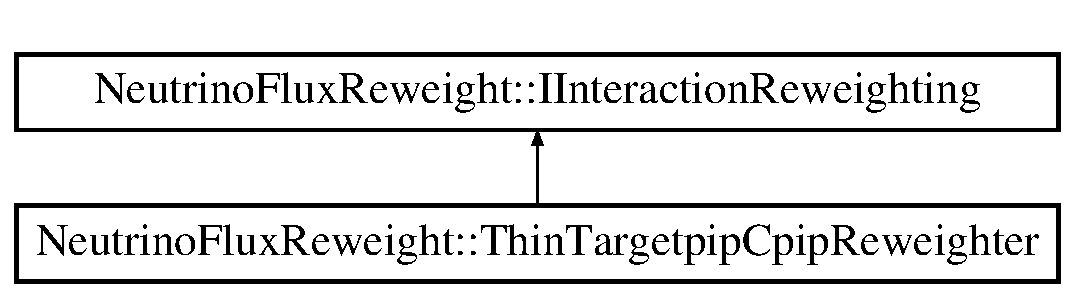
\includegraphics[height=2.000000cm]{class_neutrino_flux_reweight_1_1_thin_targetpip_cpip_reweighter}
\end{center}
\end{figure}
\subsection*{Public Member Functions}
\begin{DoxyCompactItemize}
\item 
\hyperlink{class_neutrino_flux_reweight_1_1_thin_targetpip_cpip_reweighter_a4d91e1d701f6673a84b240c75e57645b}{Thin\-Targetpip\-Cpip\-Reweighter} (int iuniv, const \hyperlink{class_neutrino_flux_reweight_1_1_parameter_table}{Parameter\-Table} \&cv\-\_\-pars, const \hyperlink{class_neutrino_flux_reweight_1_1_parameter_table}{Parameter\-Table} \&univ\-\_\-pars)
\item 
virtual \hyperlink{class_neutrino_flux_reweight_1_1_thin_targetpip_cpip_reweighter_a3568a68381ed53d1303d5eaa535eb982}{$\sim$\-Thin\-Targetpip\-Cpip\-Reweighter} ()
\item 
virtual bool \hyperlink{class_neutrino_flux_reweight_1_1_thin_targetpip_cpip_reweighter_a0a7a18f342e8c88715671e3804dbd1ca}{can\-Reweight} (const \hyperlink{class_neutrino_flux_reweight_1_1_interaction_data}{Interaction\-Data} \&aa)
\begin{DoxyCompactList}\small\item\em can the particular instance of this class reweight this interaction? \end{DoxyCompactList}\item 
virtual double \hyperlink{class_neutrino_flux_reweight_1_1_thin_targetpip_cpip_reweighter_a1491b7320847333a7b6f8b472d4e5ee3}{calculate\-Weight} (const \hyperlink{class_neutrino_flux_reweight_1_1_interaction_data}{Interaction\-Data} \&aa)
\begin{DoxyCompactList}\small\item\em calculate a weight for this interaction given the central value parameters and the parameters for this universe. The weight is something like\-: f(cv)/f(M\-C) $\ast$ f(univ)/f(cv) where cv in this case corresponds to the best value of the parameter, given the data. If univ\-\_\-pars=cv\-\_\-pars then we are calculating a central value weight \end{DoxyCompactList}\end{DoxyCompactItemize}
\subsection*{Public Attributes}
\begin{DoxyCompactItemize}
\item 
double \hyperlink{class_neutrino_flux_reweight_1_1_thin_targetpip_cpip_reweighter_a7c7cf904549d046af9ce12b44f39d92f}{data\-\_\-prod\-\_\-xs}
\item 
std\-::vector$<$ float $>$ \hyperlink{class_neutrino_flux_reweight_1_1_thin_targetpip_cpip_reweighter_a163f6f641a9673db0d5d17abd9675c20}{vbin\-\_\-data\-\_\-pip\-C\-\_\-pip}
\end{DoxyCompactItemize}
\subsection*{Private Attributes}
\begin{DoxyCompactItemize}
\item 
int \hyperlink{class_neutrino_flux_reweight_1_1_thin_targetpip_cpip_reweighter_a41ab96e7fbc624fe119247d66cf6ad70}{i\-Univ}
\item 
const \hyperlink{class_neutrino_flux_reweight_1_1_parameter_table}{Parameter\-Table} \& \hyperlink{class_neutrino_flux_reweight_1_1_thin_targetpip_cpip_reweighter_a797d9e4a1876dce2d712bd746c038d56}{cv\-Pars}
\item 
const \hyperlink{class_neutrino_flux_reweight_1_1_parameter_table}{Parameter\-Table} \& \hyperlink{class_neutrino_flux_reweight_1_1_thin_targetpip_cpip_reweighter_a9523dc5549efc3823b4cdae9236bd9f6}{univ\-Pars}
\end{DoxyCompactItemize}


\subsection{Detailed Description}


Definition at line 18 of file Thin\-Targetpip\-Cpip\-Reweighter.\-h.



\subsection{Constructor \& Destructor Documentation}
\hypertarget{class_neutrino_flux_reweight_1_1_thin_targetpip_cpip_reweighter_a4d91e1d701f6673a84b240c75e57645b}{\index{Neutrino\-Flux\-Reweight\-::\-Thin\-Targetpip\-Cpip\-Reweighter@{Neutrino\-Flux\-Reweight\-::\-Thin\-Targetpip\-Cpip\-Reweighter}!Thin\-Targetpip\-Cpip\-Reweighter@{Thin\-Targetpip\-Cpip\-Reweighter}}
\index{Thin\-Targetpip\-Cpip\-Reweighter@{Thin\-Targetpip\-Cpip\-Reweighter}!NeutrinoFluxReweight::ThinTargetpipCpipReweighter@{Neutrino\-Flux\-Reweight\-::\-Thin\-Targetpip\-Cpip\-Reweighter}}
\subsubsection[{Thin\-Targetpip\-Cpip\-Reweighter}]{\setlength{\rightskip}{0pt plus 5cm}Neutrino\-Flux\-Reweight\-::\-Thin\-Targetpip\-Cpip\-Reweighter\-::\-Thin\-Targetpip\-Cpip\-Reweighter (
\begin{DoxyParamCaption}
\item[{int}]{iuniv, }
\item[{const {\bf Parameter\-Table} \&}]{cv\-\_\-pars, }
\item[{const {\bf Parameter\-Table} \&}]{univ\-\_\-pars}
\end{DoxyParamCaption}
)}}\label{class_neutrino_flux_reweight_1_1_thin_targetpip_cpip_reweighter_a4d91e1d701f6673a84b240c75e57645b}


Definition at line 11 of file Thin\-Targetpip\-Cpip\-Reweighter.\-cpp.


\begin{DoxyCode}
11                                                                                                            
                              :\hyperlink{class_neutrino_flux_reweight_1_1_thin_targetpip_cpip_reweighter_a41ab96e7fbc624fe119247d66cf6ad70}{iUniv}(iuniv),\hyperlink{class_neutrino_flux_reweight_1_1_thin_targetpip_cpip_reweighter_a797d9e4a1876dce2d712bd746c038d56}{cvPars}(cv\_pars),\hyperlink{class_neutrino_flux_reweight_1_1_thin_targetpip_cpip_reweighter_a9523dc5549efc3823b4cdae9236bd9f6}{univPars}(univ\_pars)\{
12     
13     ThinTargetpipCpipBins* Thinbins =  \hyperlink{class_neutrino_flux_reweight_1_1_thin_targetpip_cpip_bins_aa9b4bec763ea562867a0d8ab9415f2c8}{ThinTargetpipCpipBins::getInstance}
      ();
14     
15     \hyperlink{class_neutrino_flux_reweight_1_1_thin_targetpip_cpip_reweighter_a163f6f641a9673db0d5d17abd9675c20}{vbin\_data\_pipC\_pip}.reserve(Thinbins->GetNbins\_pipC\_pip());
16     \hyperlink{class_neutrino_flux_reweight_1_1_thin_targetpip_cpip_reweighter_a7c7cf904549d046af9ce12b44f39d92f}{data\_prod\_xs} = \hyperlink{class_neutrino_flux_reweight_1_1_thin_targetpip_cpip_reweighter_a9523dc5549efc3823b4cdae9236bd9f6}{univPars}.\hyperlink{class_neutrino_flux_reweight_1_1_parameter_table_acb7dc8335b65b116f6092f2fa57ca5ed}{getParameterValue}(\textcolor{stringliteral}{"inel\_piC\_xsec\_scale"}); \textcolor{comment}{
      //bhu}
17  
18     \textcolor{keywordtype}{char} namepar[100];
19     \textcolor{keywordflow}{for}(\textcolor{keywordtype}{int} ii=0;ii<Thinbins->GetNbins\_pipC\_pip();ii++)\{
20       
21       sprintf(namepar,\textcolor{stringliteral}{"ThinTarget\_pipC\_%s\_stat\_%d"},\textcolor{stringliteral}{"pip"},ii);
22       \textcolor{keywordtype}{double} data\_cv  = \hyperlink{class_neutrino_flux_reweight_1_1_thin_targetpip_cpip_reweighter_a797d9e4a1876dce2d712bd746c038d56}{cvPars}.\hyperlink{class_neutrino_flux_reweight_1_1_parameter_table_acb7dc8335b65b116f6092f2fa57ca5ed}{getParameterValue}(std::string(namepar));
23       \textcolor{keywordtype}{double} data\_sta = \hyperlink{class_neutrino_flux_reweight_1_1_thin_targetpip_cpip_reweighter_a9523dc5549efc3823b4cdae9236bd9f6}{univPars}.\hyperlink{class_neutrino_flux_reweight_1_1_parameter_table_acb7dc8335b65b116f6092f2fa57ca5ed}{getParameterValue}(std::string(namepar));
24 \textcolor{comment}{//BHUMIKA. 29Dec, made this change of including everything}
25     sprintf(namepar,\textcolor{stringliteral}{"ThinTarget\_pipC\_%s\_sys\_%d"},\textcolor{stringliteral}{"pip"},ii);
26     \textcolor{keywordtype}{double} data\_sys = \hyperlink{class_neutrino_flux_reweight_1_1_thin_targetpip_cpip_reweighter_a9523dc5549efc3823b4cdae9236bd9f6}{univPars}.\hyperlink{class_neutrino_flux_reweight_1_1_parameter_table_acb7dc8335b65b116f6092f2fa57ca5ed}{getParameterValue}(std::string(namepar));
27 
28     \hyperlink{class_neutrino_flux_reweight_1_1_thin_targetpip_cpip_reweighter_a163f6f641a9673db0d5d17abd9675c20}{vbin\_data\_pipC\_pip}.push\_back(data\_sys + data\_sta - data\_cv);
29      
30     \textcolor{comment}{//  vbin\_data\_pipC\_pip.push\_back(data\_sta);}
31     \}
32  \textcolor{comment}{//Bhumika, to print the elements of this vector}
33 \textcolor{comment}{//std::cout<<"Bhumika printing this vector"<<std::endl; }
34 \textcolor{comment}{//std::cout << "Vector elements: ";}
35 \textcolor{comment}{//if (iuniv=35)\{}
36  \textcolor{keywordflow}{for} (\textcolor{keywordtype}{int} i = 0; i < \hyperlink{class_neutrino_flux_reweight_1_1_thin_targetpip_cpip_reweighter_a163f6f641a9673db0d5d17abd9675c20}{vbin\_data\_pipC\_pip}.size(); ++i) \{
37   std::cout << \hyperlink{class_neutrino_flux_reweight_1_1_thin_targetpip_cpip_reweighter_a163f6f641a9673db0d5d17abd9675c20}{vbin\_data\_pipC\_pip}[i] << \textcolor{stringliteral}{" "};\}
38           
39 \textcolor{comment}{//\}}
40 \}
\end{DoxyCode}
\hypertarget{class_neutrino_flux_reweight_1_1_thin_targetpip_cpip_reweighter_a3568a68381ed53d1303d5eaa535eb982}{\index{Neutrino\-Flux\-Reweight\-::\-Thin\-Targetpip\-Cpip\-Reweighter@{Neutrino\-Flux\-Reweight\-::\-Thin\-Targetpip\-Cpip\-Reweighter}!$\sim$\-Thin\-Targetpip\-Cpip\-Reweighter@{$\sim$\-Thin\-Targetpip\-Cpip\-Reweighter}}
\index{$\sim$\-Thin\-Targetpip\-Cpip\-Reweighter@{$\sim$\-Thin\-Targetpip\-Cpip\-Reweighter}!NeutrinoFluxReweight::ThinTargetpipCpipReweighter@{Neutrino\-Flux\-Reweight\-::\-Thin\-Targetpip\-Cpip\-Reweighter}}
\subsubsection[{$\sim$\-Thin\-Targetpip\-Cpip\-Reweighter}]{\setlength{\rightskip}{0pt plus 5cm}Neutrino\-Flux\-Reweight\-::\-Thin\-Targetpip\-Cpip\-Reweighter\-::$\sim$\-Thin\-Targetpip\-Cpip\-Reweighter (
\begin{DoxyParamCaption}
{}
\end{DoxyParamCaption}
)\hspace{0.3cm}{\ttfamily [virtual]}}}\label{class_neutrino_flux_reweight_1_1_thin_targetpip_cpip_reweighter_a3568a68381ed53d1303d5eaa535eb982}


Definition at line 42 of file Thin\-Targetpip\-Cpip\-Reweighter.\-cpp.


\begin{DoxyCode}
42                                                            \{
43     
44   \}
\end{DoxyCode}


\subsection{Member Function Documentation}
\hypertarget{class_neutrino_flux_reweight_1_1_thin_targetpip_cpip_reweighter_a1491b7320847333a7b6f8b472d4e5ee3}{\index{Neutrino\-Flux\-Reweight\-::\-Thin\-Targetpip\-Cpip\-Reweighter@{Neutrino\-Flux\-Reweight\-::\-Thin\-Targetpip\-Cpip\-Reweighter}!calculate\-Weight@{calculate\-Weight}}
\index{calculate\-Weight@{calculate\-Weight}!NeutrinoFluxReweight::ThinTargetpipCpipReweighter@{Neutrino\-Flux\-Reweight\-::\-Thin\-Targetpip\-Cpip\-Reweighter}}
\subsubsection[{calculate\-Weight}]{\setlength{\rightskip}{0pt plus 5cm}double Neutrino\-Flux\-Reweight\-::\-Thin\-Targetpip\-Cpip\-Reweighter\-::calculate\-Weight (
\begin{DoxyParamCaption}
\item[{const {\bf Interaction\-Data} \&}]{inter\-\_\-data}
\end{DoxyParamCaption}
)\hspace{0.3cm}{\ttfamily [virtual]}}}\label{class_neutrino_flux_reweight_1_1_thin_targetpip_cpip_reweighter_a1491b7320847333a7b6f8b472d4e5ee3}


calculate a weight for this interaction given the central value parameters and the parameters for this universe. The weight is something like\-: f(cv)/f(M\-C) $\ast$ f(univ)/f(cv) where cv in this case corresponds to the best value of the parameter, given the data. If univ\-\_\-pars=cv\-\_\-pars then we are calculating a central value weight 



Implements \hyperlink{class_neutrino_flux_reweight_1_1_i_interaction_reweighting_a49b0d73e778411d629205d23575703c3}{Neutrino\-Flux\-Reweight\-::\-I\-Interaction\-Reweighting}.



Definition at line 64 of file Thin\-Targetpip\-Cpip\-Reweighter.\-cpp.


\begin{DoxyCode}
64                                                                               \{
65 
66     \textcolor{keywordtype}{double} wgt = 1.0;
67     \textcolor{keywordtype}{double} low\_value = 1.e-18;     \textcolor{comment}{//BHU, Copied it, but how do we get this value}
68 
69     \textcolor{keywordtype}{bool} right\_inc = aa.Inc\_pdg == 211; 
70     \textcolor{keywordtype}{bool} right\_prod = aa.Prod\_pdg == 211;
71    \textcolor{comment}{// bool right\_energy = aa.Inc\_P >= 12;}
72    
73     ThinTargetpipCpipBins*  Thinbins =  \hyperlink{class_neutrino_flux_reweight_1_1_thin_targetpip_cpip_bins_aa9b4bec763ea562867a0d8ab9415f2c8}{ThinTargetpipCpipBins::getInstance}
      ();
74     ThinTargetpipCpipMC*  mc =  \hyperlink{class_neutrino_flux_reweight_1_1_thin_targetpip_cpip_m_c_aeeb5ad3ed4803b1122286f49d1897729}{ThinTargetpipCpipMC::getInstance}();
75    \textcolor{comment}{//Getting the MC:}
76 
77   \textcolor{keywordtype}{double} pipC\_pip\_cv = mc->getMCval(aa.Prod\_P, aa.Theta, aa.Inc\_pdg, aa.Prod\_pdg);    \textcolor{comment}{//BHU.Edit this}
78 \textcolor{comment}{//  std::cout<<"The central value from mc is: "<<pipC\_pip\_cv<< std::endl;}
79     
80   \textcolor{keywordflow}{if}(pipC\_pip\_cv<1.e-18)\{
81   std::cout<<\textcolor{stringliteral}{"LOW MC VAL: "}<<pipC\_pip\_cv<<std::endl;
82   
83   \textcolor{comment}{//std::cout<<"The central value from mc is: "<<pipC\_pip\_cv<< std::endl;}
84 
85   \textcolor{keywordflow}{return} 1.0;\}
86   \textcolor{comment}{//getting data bin value}
87     \textcolor{keywordtype}{int} bin      = Thinbins->pipC\_pip\_BinID(aa.Prod\_P,aa.Theta, aa.Inc\_pdg, aa.Prod\_pdg);
88   \textcolor{comment}{// std::cout<<"The bin number from data bins is: "<<bin<<std::endl;  }
89   \textcolor{keywordflow}{if}(bin<0 || bin>200)\{
90   std::cout<<\textcolor{stringliteral}{"BINID from data is less than ZERO or greater than 200, incident mom is:"} <<aa.Inc\_P<<\textcolor{stringliteral}{"Theta
       value is "} <<aa.Theta<<std::endl;
91      \textcolor{keywordflow}{return} 1.0;\}
92 \textcolor{comment}{//Calculating the weight}
93   \textcolor{keywordflow}{if}(aa.Prod\_pdg == 211 && bin>=0 && aa.Inc\_pdg==211 && aa.Inc\_P >= 12)     \textcolor{comment}{//BHUMIKA, adding new energy
       condition}
94     wgt = \hyperlink{class_neutrino_flux_reweight_1_1_thin_targetpip_cpip_reweighter_a163f6f641a9673db0d5d17abd9675c20}{vbin\_data\_pipC\_pip}[bin]/pipC\_pip\_cv;
95   std::cout<<\textcolor{stringliteral}{"The bin content from data for this particular bin is:"}<< 
      \hyperlink{class_neutrino_flux_reweight_1_1_thin_targetpip_cpip_reweighter_a163f6f641a9673db0d5d17abd9675c20}{vbin\_data\_pipC\_pip}[bin] <<std::endl;
96   std::cout<<\textcolor{stringliteral}{"Weight by NA61 reweighter using Statistical only is : "}<<wgt<<std::endl;
97     \textcolor{keywordflow}{if}(wgt<0)\{std::cout<<\textcolor{stringliteral}{"NA61 check wgt:"}<<\textcolor{stringliteral}{"The univ no"}<<\hyperlink{class_neutrino_flux_reweight_1_1_thin_targetpip_cpip_reweighter_a41ab96e7fbc624fe119247d66cf6ad70}{iUniv}<<\textcolor{stringliteral}{"mom of produced "}<<aa.Prod\_P<<\textcolor{stringliteral}{"mom
       of incident "}<<aa.Theta<<std::endl;
98     \}
99     
100     \textcolor{keywordflow}{if}(wgt>10)\{
101       std::cout<<\textcolor{stringliteral}{"BIG WGT IN TTMESONINC "}<<\hyperlink{class_neutrino_flux_reweight_1_1_thin_targetpip_cpip_reweighter_a41ab96e7fbc624fe119247d66cf6ad70}{iUniv}<<\textcolor{stringliteral}{" "}<<wgt<<\textcolor{stringliteral}{" "}<<aa.Prod\_P<<\textcolor{stringliteral}{" "}<<aa.Theta<<\textcolor{stringliteral}{" "}<<aa.
      Inc\_pdg<<\textcolor{stringliteral}{" "}<<aa.Prod\_pdg<<std::endl;
102       \textcolor{keywordflow}{return} 1.0;
103     \}
104     \textcolor{keywordflow}{return} wgt;
105 
106   \}
\end{DoxyCode}
\hypertarget{class_neutrino_flux_reweight_1_1_thin_targetpip_cpip_reweighter_a0a7a18f342e8c88715671e3804dbd1ca}{\index{Neutrino\-Flux\-Reweight\-::\-Thin\-Targetpip\-Cpip\-Reweighter@{Neutrino\-Flux\-Reweight\-::\-Thin\-Targetpip\-Cpip\-Reweighter}!can\-Reweight@{can\-Reweight}}
\index{can\-Reweight@{can\-Reweight}!NeutrinoFluxReweight::ThinTargetpipCpipReweighter@{Neutrino\-Flux\-Reweight\-::\-Thin\-Targetpip\-Cpip\-Reweighter}}
\subsubsection[{can\-Reweight}]{\setlength{\rightskip}{0pt plus 5cm}bool Neutrino\-Flux\-Reweight\-::\-Thin\-Targetpip\-Cpip\-Reweighter\-::can\-Reweight (
\begin{DoxyParamCaption}
\item[{const {\bf Interaction\-Data} \&}]{aa}
\end{DoxyParamCaption}
)\hspace{0.3cm}{\ttfamily [virtual]}}}\label{class_neutrino_flux_reweight_1_1_thin_targetpip_cpip_reweighter_a0a7a18f342e8c88715671e3804dbd1ca}


can the particular instance of this class reweight this interaction? 



Implements \hyperlink{class_neutrino_flux_reweight_1_1_i_interaction_reweighting_aa3d1d3f37a93b02e447cf5eca333ac8d}{Neutrino\-Flux\-Reweight\-::\-I\-Interaction\-Reweighting}.



Definition at line 45 of file Thin\-Targetpip\-Cpip\-Reweighter.\-cpp.


\begin{DoxyCode}
45                                                                         \{
46    
47    \textcolor{keywordflow}{if}(aa.Proc.find(\textcolor{stringliteral}{"Inelastic"})>100)\{       \textcolor{comment}{//BHU,WHY THIS CRITERIA?? DO I need to use this?}
48      
49     \textcolor{comment}{// std::cout<<"The interaction details"<<"Inc\_mom: "<<aa.Inc\_P <<"prod\_mom: "<<aa.Prod\_P <<"Inc\_pdg:
       "<< aa.Inc\_pdg <<"prod\_pdg: "<< aa.Prod\_pdg<< std::endl;}
50    \textcolor{comment}{//  std::cout<<"The details of process are(BHUMI):"<< aa.Proc<<std::endl;}
51     \textcolor{keywordflow}{return} \textcolor{keyword}{false}; 
52      \} 
53     ThinTargetpipCpipBins*  Thinbins =  \hyperlink{class_neutrino_flux_reweight_1_1_thin_targetpip_cpip_bins_aa9b4bec763ea562867a0d8ab9415f2c8}{ThinTargetpipCpipBins::getInstance}
      ();
54     \textcolor{keywordtype}{int} bin = Thinbins->pipC\_pip\_BinID(aa.Prod\_P,aa.Theta,aa.Inc\_pdg,aa.Prod\_pdg); \textcolor{comment}{//USING THESE VARIABLES
       AS WE HAD DATA IN THESE}
55    
56    \textcolor{comment}{// bool is\_pipinc = (aa.Inc\_pdg ==211 && aa.Prod\_pdg == 211);}
57      \textcolor{keywordtype}{bool} is\_pipinc = (aa.Inc\_pdg ==211 && aa.Prod\_pdg == 211 && aa.Inc\_P >= 12);  \textcolor{comment}{//BHUMIKA ADDING NEW
       CONDITION}
58 
59     \textcolor{keywordflow}{if}(is\_pipinc)\textcolor{keywordflow}{return} \textcolor{keyword}{true};
60     \textcolor{keywordflow}{else} \textcolor{keywordflow}{return} \textcolor{keyword}{false};
61     
62   \}
\end{DoxyCode}


\subsection{Member Data Documentation}
\hypertarget{class_neutrino_flux_reweight_1_1_thin_targetpip_cpip_reweighter_a797d9e4a1876dce2d712bd746c038d56}{\index{Neutrino\-Flux\-Reweight\-::\-Thin\-Targetpip\-Cpip\-Reweighter@{Neutrino\-Flux\-Reweight\-::\-Thin\-Targetpip\-Cpip\-Reweighter}!cv\-Pars@{cv\-Pars}}
\index{cv\-Pars@{cv\-Pars}!NeutrinoFluxReweight::ThinTargetpipCpipReweighter@{Neutrino\-Flux\-Reweight\-::\-Thin\-Targetpip\-Cpip\-Reweighter}}
\subsubsection[{cv\-Pars}]{\setlength{\rightskip}{0pt plus 5cm}const {\bf Parameter\-Table}\& Neutrino\-Flux\-Reweight\-::\-Thin\-Targetpip\-Cpip\-Reweighter\-::cv\-Pars\hspace{0.3cm}{\ttfamily [private]}}}\label{class_neutrino_flux_reweight_1_1_thin_targetpip_cpip_reweighter_a797d9e4a1876dce2d712bd746c038d56}


Definition at line 32 of file Thin\-Targetpip\-Cpip\-Reweighter.\-h.

\hypertarget{class_neutrino_flux_reweight_1_1_thin_targetpip_cpip_reweighter_a7c7cf904549d046af9ce12b44f39d92f}{\index{Neutrino\-Flux\-Reweight\-::\-Thin\-Targetpip\-Cpip\-Reweighter@{Neutrino\-Flux\-Reweight\-::\-Thin\-Targetpip\-Cpip\-Reweighter}!data\-\_\-prod\-\_\-xs@{data\-\_\-prod\-\_\-xs}}
\index{data\-\_\-prod\-\_\-xs@{data\-\_\-prod\-\_\-xs}!NeutrinoFluxReweight::ThinTargetpipCpipReweighter@{Neutrino\-Flux\-Reweight\-::\-Thin\-Targetpip\-Cpip\-Reweighter}}
\subsubsection[{data\-\_\-prod\-\_\-xs}]{\setlength{\rightskip}{0pt plus 5cm}double Neutrino\-Flux\-Reweight\-::\-Thin\-Targetpip\-Cpip\-Reweighter\-::data\-\_\-prod\-\_\-xs}}\label{class_neutrino_flux_reweight_1_1_thin_targetpip_cpip_reweighter_a7c7cf904549d046af9ce12b44f39d92f}


Definition at line 26 of file Thin\-Targetpip\-Cpip\-Reweighter.\-h.

\hypertarget{class_neutrino_flux_reweight_1_1_thin_targetpip_cpip_reweighter_a41ab96e7fbc624fe119247d66cf6ad70}{\index{Neutrino\-Flux\-Reweight\-::\-Thin\-Targetpip\-Cpip\-Reweighter@{Neutrino\-Flux\-Reweight\-::\-Thin\-Targetpip\-Cpip\-Reweighter}!i\-Univ@{i\-Univ}}
\index{i\-Univ@{i\-Univ}!NeutrinoFluxReweight::ThinTargetpipCpipReweighter@{Neutrino\-Flux\-Reweight\-::\-Thin\-Targetpip\-Cpip\-Reweighter}}
\subsubsection[{i\-Univ}]{\setlength{\rightskip}{0pt plus 5cm}int Neutrino\-Flux\-Reweight\-::\-Thin\-Targetpip\-Cpip\-Reweighter\-::i\-Univ\hspace{0.3cm}{\ttfamily [private]}}}\label{class_neutrino_flux_reweight_1_1_thin_targetpip_cpip_reweighter_a41ab96e7fbc624fe119247d66cf6ad70}


Definition at line 31 of file Thin\-Targetpip\-Cpip\-Reweighter.\-h.

\hypertarget{class_neutrino_flux_reweight_1_1_thin_targetpip_cpip_reweighter_a9523dc5549efc3823b4cdae9236bd9f6}{\index{Neutrino\-Flux\-Reweight\-::\-Thin\-Targetpip\-Cpip\-Reweighter@{Neutrino\-Flux\-Reweight\-::\-Thin\-Targetpip\-Cpip\-Reweighter}!univ\-Pars@{univ\-Pars}}
\index{univ\-Pars@{univ\-Pars}!NeutrinoFluxReweight::ThinTargetpipCpipReweighter@{Neutrino\-Flux\-Reweight\-::\-Thin\-Targetpip\-Cpip\-Reweighter}}
\subsubsection[{univ\-Pars}]{\setlength{\rightskip}{0pt plus 5cm}const {\bf Parameter\-Table}\& Neutrino\-Flux\-Reweight\-::\-Thin\-Targetpip\-Cpip\-Reweighter\-::univ\-Pars\hspace{0.3cm}{\ttfamily [private]}}}\label{class_neutrino_flux_reweight_1_1_thin_targetpip_cpip_reweighter_a9523dc5549efc3823b4cdae9236bd9f6}


Definition at line 33 of file Thin\-Targetpip\-Cpip\-Reweighter.\-h.

\hypertarget{class_neutrino_flux_reweight_1_1_thin_targetpip_cpip_reweighter_a163f6f641a9673db0d5d17abd9675c20}{\index{Neutrino\-Flux\-Reweight\-::\-Thin\-Targetpip\-Cpip\-Reweighter@{Neutrino\-Flux\-Reweight\-::\-Thin\-Targetpip\-Cpip\-Reweighter}!vbin\-\_\-data\-\_\-pip\-C\-\_\-pip@{vbin\-\_\-data\-\_\-pip\-C\-\_\-pip}}
\index{vbin\-\_\-data\-\_\-pip\-C\-\_\-pip@{vbin\-\_\-data\-\_\-pip\-C\-\_\-pip}!NeutrinoFluxReweight::ThinTargetpipCpipReweighter@{Neutrino\-Flux\-Reweight\-::\-Thin\-Targetpip\-Cpip\-Reweighter}}
\subsubsection[{vbin\-\_\-data\-\_\-pip\-C\-\_\-pip}]{\setlength{\rightskip}{0pt plus 5cm}std\-::vector$<$float$>$ Neutrino\-Flux\-Reweight\-::\-Thin\-Targetpip\-Cpip\-Reweighter\-::vbin\-\_\-data\-\_\-pip\-C\-\_\-pip}}\label{class_neutrino_flux_reweight_1_1_thin_targetpip_cpip_reweighter_a163f6f641a9673db0d5d17abd9675c20}


Definition at line 27 of file Thin\-Targetpip\-Cpip\-Reweighter.\-h.



The documentation for this class was generated from the following files\-:\begin{DoxyCompactItemize}
\item 
include/\hyperlink{_thin_targetpip_cpip_reweighter_8h}{Thin\-Targetpip\-Cpip\-Reweighter.\-h}\item 
src/\hyperlink{_thin_targetpip_cpip_reweighter_8cpp}{Thin\-Targetpip\-Cpip\-Reweighter.\-cpp}\end{DoxyCompactItemize}

\hypertarget{class_neutrino_flux_reweight_1_1_thin_targetpip_c_reweighter}{\section{Neutrino\-Flux\-Reweight\-:\-:Thin\-Targetpip\-C\-Reweighter Class Reference}
\label{class_neutrino_flux_reweight_1_1_thin_targetpip_c_reweighter}\index{Neutrino\-Flux\-Reweight\-::\-Thin\-Targetpip\-C\-Reweighter@{Neutrino\-Flux\-Reweight\-::\-Thin\-Targetpip\-C\-Reweighter}}
}


Reweighter of N\-A61 pip Interactions.  




{\ttfamily \#include $<$Thin\-Targetpip\-C\-Reweighter.\-h$>$}

Inheritance diagram for Neutrino\-Flux\-Reweight\-:\-:Thin\-Targetpip\-C\-Reweighter\-:\begin{figure}[H]
\begin{center}
\leavevmode
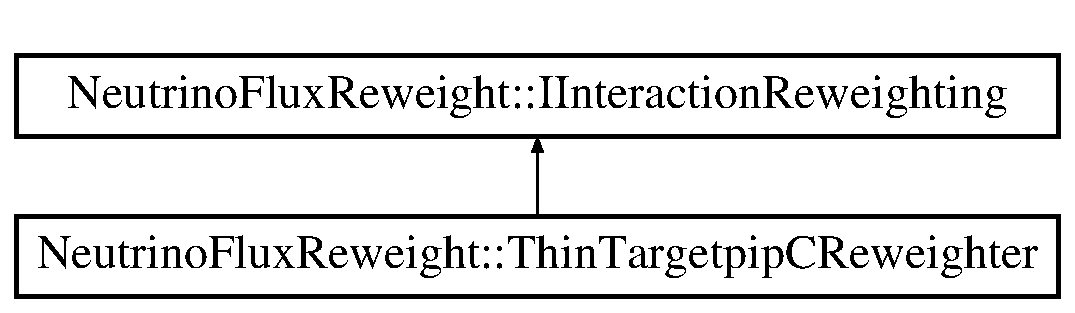
\includegraphics[height=2.000000cm]{class_neutrino_flux_reweight_1_1_thin_targetpip_c_reweighter}
\end{center}
\end{figure}
\subsection*{Public Member Functions}
\begin{DoxyCompactItemize}
\item 
\hyperlink{class_neutrino_flux_reweight_1_1_thin_targetpip_c_reweighter_ada13aac28762c55f4c58fd40e893ca40}{Thin\-Targetpip\-C\-Reweighter} (int iuniv, const \hyperlink{class_neutrino_flux_reweight_1_1_parameter_table}{Parameter\-Table} \&cv\-\_\-pars, const \hyperlink{class_neutrino_flux_reweight_1_1_parameter_table}{Parameter\-Table} \&univ\-\_\-pars)
\item 
virtual \hyperlink{class_neutrino_flux_reweight_1_1_thin_targetpip_c_reweighter_a28cc620d0c0d6b363590ee270e81a3f5}{$\sim$\-Thin\-Targetpip\-C\-Reweighter} ()
\item 
virtual bool \hyperlink{class_neutrino_flux_reweight_1_1_thin_targetpip_c_reweighter_a85dfb364850ec5af9b58cdff4c37c678}{can\-Reweight} (const \hyperlink{class_neutrino_flux_reweight_1_1_interaction_data}{Interaction\-Data} \&aa)
\begin{DoxyCompactList}\small\item\em can the particular instance of this class reweight this interaction? \end{DoxyCompactList}\item 
virtual double \hyperlink{class_neutrino_flux_reweight_1_1_thin_targetpip_c_reweighter_a6941429f810ddcc72aa979e829da3314}{calculate\-Weight} (const \hyperlink{class_neutrino_flux_reweight_1_1_interaction_data}{Interaction\-Data} \&aa)
\begin{DoxyCompactList}\small\item\em calculate a weight for this interaction given the central value parameters and the parameters for this universe. The weight is something like\-: f(cv)/f(M\-C) $\ast$ f(univ)/f(cv) where cv in this case corresponds to the best value of the parameter, given the data. If univ\-\_\-pars=cv\-\_\-pars then we are calculating a central value weight \end{DoxyCompactList}\end{DoxyCompactItemize}
\subsection*{Private Attributes}
\begin{DoxyCompactItemize}
\item 
int \hyperlink{class_neutrino_flux_reweight_1_1_thin_targetpip_c_reweighter_a97d91aff2a76990d435c1534a7d29dca}{i\-Univ}
\item 
const \hyperlink{class_neutrino_flux_reweight_1_1_parameter_table}{Parameter\-Table} \& \hyperlink{class_neutrino_flux_reweight_1_1_thin_targetpip_c_reweighter_af5d2120c06647661015daae96c40f130}{cv\-Pars}
\item 
const \hyperlink{class_neutrino_flux_reweight_1_1_parameter_table}{Parameter\-Table} \& \hyperlink{class_neutrino_flux_reweight_1_1_thin_targetpip_c_reweighter_a5fb560293bea225254092a20c2261008}{univ\-Pars}
\end{DoxyCompactItemize}


\subsection{Detailed Description}
Reweighter of N\-A61 pip Interactions. 

Definition at line 19 of file Thin\-Targetpip\-C\-Reweighter.\-h.



\subsection{Constructor \& Destructor Documentation}
\hypertarget{class_neutrino_flux_reweight_1_1_thin_targetpip_c_reweighter_ada13aac28762c55f4c58fd40e893ca40}{\index{Neutrino\-Flux\-Reweight\-::\-Thin\-Targetpip\-C\-Reweighter@{Neutrino\-Flux\-Reweight\-::\-Thin\-Targetpip\-C\-Reweighter}!Thin\-Targetpip\-C\-Reweighter@{Thin\-Targetpip\-C\-Reweighter}}
\index{Thin\-Targetpip\-C\-Reweighter@{Thin\-Targetpip\-C\-Reweighter}!NeutrinoFluxReweight::ThinTargetpipCReweighter@{Neutrino\-Flux\-Reweight\-::\-Thin\-Targetpip\-C\-Reweighter}}
\subsubsection[{Thin\-Targetpip\-C\-Reweighter}]{\setlength{\rightskip}{0pt plus 5cm}Neutrino\-Flux\-Reweight\-::\-Thin\-Targetpip\-C\-Reweighter\-::\-Thin\-Targetpip\-C\-Reweighter (
\begin{DoxyParamCaption}
\item[{int}]{iuniv, }
\item[{const {\bf Parameter\-Table} \&}]{cv\-\_\-pars, }
\item[{const {\bf Parameter\-Table} \&}]{univ\-\_\-pars}
\end{DoxyParamCaption}
)}}\label{class_neutrino_flux_reweight_1_1_thin_targetpip_c_reweighter_ada13aac28762c55f4c58fd40e893ca40}


Definition at line 7 of file Thin\-Targetpip\-C\-Reweighter.\-cpp.


\begin{DoxyCode}
7                                                                                                            
                        :\hyperlink{class_neutrino_flux_reweight_1_1_thin_targetpip_c_reweighter_a97d91aff2a76990d435c1534a7d29dca}{iUniv}(iuniv),\hyperlink{class_neutrino_flux_reweight_1_1_thin_targetpip_c_reweighter_af5d2120c06647661015daae96c40f130}{cvPars}(cv\_pars),\hyperlink{class_neutrino_flux_reweight_1_1_thin_targetpip_c_reweighter_a5fb560293bea225254092a20c2261008}{univPars}(univ\_pars)\{
8     
9     ThinTargetBins* Thinbins =  \hyperlink{class_neutrino_flux_reweight_1_1_thin_target_bins_aeff5cf7220dd08322f5abac2cbc7ff33}{ThinTargetBins::getInstance}();
10     
11     
12     \textcolor{comment}{//1 incident particles, 8 produced particles:}
13     
14  \}
\end{DoxyCode}
\hypertarget{class_neutrino_flux_reweight_1_1_thin_targetpip_c_reweighter_a28cc620d0c0d6b363590ee270e81a3f5}{\index{Neutrino\-Flux\-Reweight\-::\-Thin\-Targetpip\-C\-Reweighter@{Neutrino\-Flux\-Reweight\-::\-Thin\-Targetpip\-C\-Reweighter}!$\sim$\-Thin\-Targetpip\-C\-Reweighter@{$\sim$\-Thin\-Targetpip\-C\-Reweighter}}
\index{$\sim$\-Thin\-Targetpip\-C\-Reweighter@{$\sim$\-Thin\-Targetpip\-C\-Reweighter}!NeutrinoFluxReweight::ThinTargetpipCReweighter@{Neutrino\-Flux\-Reweight\-::\-Thin\-Targetpip\-C\-Reweighter}}
\subsubsection[{$\sim$\-Thin\-Targetpip\-C\-Reweighter}]{\setlength{\rightskip}{0pt plus 5cm}Neutrino\-Flux\-Reweight\-::\-Thin\-Targetpip\-C\-Reweighter\-::$\sim$\-Thin\-Targetpip\-C\-Reweighter (
\begin{DoxyParamCaption}
{}
\end{DoxyParamCaption}
)\hspace{0.3cm}{\ttfamily [virtual]}}}\label{class_neutrino_flux_reweight_1_1_thin_targetpip_c_reweighter_a28cc620d0c0d6b363590ee270e81a3f5}


Definition at line 16 of file Thin\-Targetpip\-C\-Reweighter.\-cpp.


\begin{DoxyCode}
16                                                      \{
17     
18   \}
\end{DoxyCode}


\subsection{Member Function Documentation}
\hypertarget{class_neutrino_flux_reweight_1_1_thin_targetpip_c_reweighter_a6941429f810ddcc72aa979e829da3314}{\index{Neutrino\-Flux\-Reweight\-::\-Thin\-Targetpip\-C\-Reweighter@{Neutrino\-Flux\-Reweight\-::\-Thin\-Targetpip\-C\-Reweighter}!calculate\-Weight@{calculate\-Weight}}
\index{calculate\-Weight@{calculate\-Weight}!NeutrinoFluxReweight::ThinTargetpipCReweighter@{Neutrino\-Flux\-Reweight\-::\-Thin\-Targetpip\-C\-Reweighter}}
\subsubsection[{calculate\-Weight}]{\setlength{\rightskip}{0pt plus 5cm}double Neutrino\-Flux\-Reweight\-::\-Thin\-Targetpip\-C\-Reweighter\-::calculate\-Weight (
\begin{DoxyParamCaption}
\item[{const {\bf Interaction\-Data} \&}]{inter\-\_\-data}
\end{DoxyParamCaption}
)\hspace{0.3cm}{\ttfamily [virtual]}}}\label{class_neutrino_flux_reweight_1_1_thin_targetpip_c_reweighter_a6941429f810ddcc72aa979e829da3314}


calculate a weight for this interaction given the central value parameters and the parameters for this universe. The weight is something like\-: f(cv)/f(M\-C) $\ast$ f(univ)/f(cv) where cv in this case corresponds to the best value of the parameter, given the data. If univ\-\_\-pars=cv\-\_\-pars then we are calculating a central value weight 



Implements \hyperlink{class_neutrino_flux_reweight_1_1_i_interaction_reweighting_a49b0d73e778411d629205d23575703c3}{Neutrino\-Flux\-Reweight\-::\-I\-Interaction\-Reweighting}.



Definition at line 26 of file Thin\-Targetpip\-C\-Reweighter.\-cpp.


\begin{DoxyCode}
26                                                                            \{
27 
28     \textcolor{keywordtype}{double} wgt = 1.0;
29    
30     \textcolor{keywordflow}{return} wgt;
31 
32   \}
\end{DoxyCode}
\hypertarget{class_neutrino_flux_reweight_1_1_thin_targetpip_c_reweighter_a85dfb364850ec5af9b58cdff4c37c678}{\index{Neutrino\-Flux\-Reweight\-::\-Thin\-Targetpip\-C\-Reweighter@{Neutrino\-Flux\-Reweight\-::\-Thin\-Targetpip\-C\-Reweighter}!can\-Reweight@{can\-Reweight}}
\index{can\-Reweight@{can\-Reweight}!NeutrinoFluxReweight::ThinTargetpipCReweighter@{Neutrino\-Flux\-Reweight\-::\-Thin\-Targetpip\-C\-Reweighter}}
\subsubsection[{can\-Reweight}]{\setlength{\rightskip}{0pt plus 5cm}bool Neutrino\-Flux\-Reweight\-::\-Thin\-Targetpip\-C\-Reweighter\-::can\-Reweight (
\begin{DoxyParamCaption}
\item[{const {\bf Interaction\-Data} \&}]{aa}
\end{DoxyParamCaption}
)\hspace{0.3cm}{\ttfamily [virtual]}}}\label{class_neutrino_flux_reweight_1_1_thin_targetpip_c_reweighter_a85dfb364850ec5af9b58cdff4c37c678}


can the particular instance of this class reweight this interaction? 



Implements \hyperlink{class_neutrino_flux_reweight_1_1_i_interaction_reweighting_aa3d1d3f37a93b02e447cf5eca333ac8d}{Neutrino\-Flux\-Reweight\-::\-I\-Interaction\-Reweighting}.



Definition at line 19 of file Thin\-Targetpip\-C\-Reweighter.\-cpp.


\begin{DoxyCode}
19                                                                      \{
20     
21   
22     \textcolor{keywordflow}{return} \textcolor{keyword}{false};
23     
24   \}
\end{DoxyCode}


\subsection{Member Data Documentation}
\hypertarget{class_neutrino_flux_reweight_1_1_thin_targetpip_c_reweighter_af5d2120c06647661015daae96c40f130}{\index{Neutrino\-Flux\-Reweight\-::\-Thin\-Targetpip\-C\-Reweighter@{Neutrino\-Flux\-Reweight\-::\-Thin\-Targetpip\-C\-Reweighter}!cv\-Pars@{cv\-Pars}}
\index{cv\-Pars@{cv\-Pars}!NeutrinoFluxReweight::ThinTargetpipCReweighter@{Neutrino\-Flux\-Reweight\-::\-Thin\-Targetpip\-C\-Reweighter}}
\subsubsection[{cv\-Pars}]{\setlength{\rightskip}{0pt plus 5cm}const {\bf Parameter\-Table}\& Neutrino\-Flux\-Reweight\-::\-Thin\-Targetpip\-C\-Reweighter\-::cv\-Pars\hspace{0.3cm}{\ttfamily [private]}}}\label{class_neutrino_flux_reweight_1_1_thin_targetpip_c_reweighter_af5d2120c06647661015daae96c40f130}


Definition at line 29 of file Thin\-Targetpip\-C\-Reweighter.\-h.

\hypertarget{class_neutrino_flux_reweight_1_1_thin_targetpip_c_reweighter_a97d91aff2a76990d435c1534a7d29dca}{\index{Neutrino\-Flux\-Reweight\-::\-Thin\-Targetpip\-C\-Reweighter@{Neutrino\-Flux\-Reweight\-::\-Thin\-Targetpip\-C\-Reweighter}!i\-Univ@{i\-Univ}}
\index{i\-Univ@{i\-Univ}!NeutrinoFluxReweight::ThinTargetpipCReweighter@{Neutrino\-Flux\-Reweight\-::\-Thin\-Targetpip\-C\-Reweighter}}
\subsubsection[{i\-Univ}]{\setlength{\rightskip}{0pt plus 5cm}int Neutrino\-Flux\-Reweight\-::\-Thin\-Targetpip\-C\-Reweighter\-::i\-Univ\hspace{0.3cm}{\ttfamily [private]}}}\label{class_neutrino_flux_reweight_1_1_thin_targetpip_c_reweighter_a97d91aff2a76990d435c1534a7d29dca}


Definition at line 28 of file Thin\-Targetpip\-C\-Reweighter.\-h.

\hypertarget{class_neutrino_flux_reweight_1_1_thin_targetpip_c_reweighter_a5fb560293bea225254092a20c2261008}{\index{Neutrino\-Flux\-Reweight\-::\-Thin\-Targetpip\-C\-Reweighter@{Neutrino\-Flux\-Reweight\-::\-Thin\-Targetpip\-C\-Reweighter}!univ\-Pars@{univ\-Pars}}
\index{univ\-Pars@{univ\-Pars}!NeutrinoFluxReweight::ThinTargetpipCReweighter@{Neutrino\-Flux\-Reweight\-::\-Thin\-Targetpip\-C\-Reweighter}}
\subsubsection[{univ\-Pars}]{\setlength{\rightskip}{0pt plus 5cm}const {\bf Parameter\-Table}\& Neutrino\-Flux\-Reweight\-::\-Thin\-Targetpip\-C\-Reweighter\-::univ\-Pars\hspace{0.3cm}{\ttfamily [private]}}}\label{class_neutrino_flux_reweight_1_1_thin_targetpip_c_reweighter_a5fb560293bea225254092a20c2261008}


Definition at line 30 of file Thin\-Targetpip\-C\-Reweighter.\-h.



The documentation for this class was generated from the following files\-:\begin{DoxyCompactItemize}
\item 
include/\hyperlink{_thin_targetpip_c_reweighter_8h}{Thin\-Targetpip\-C\-Reweighter.\-h}\item 
src/\hyperlink{_thin_targetpip_c_reweighter_8cpp}{Thin\-Targetpip\-C\-Reweighter.\-cpp}\end{DoxyCompactItemize}

\chapter{File Documentation}
\hypertarget{_absorption_d_p_i_p_reweighter_8h}{\section{include/\-Absorption\-D\-P\-I\-P\-Reweighter.h File Reference}
\label{_absorption_d_p_i_p_reweighter_8h}\index{include/\-Absorption\-D\-P\-I\-P\-Reweighter.\-h@{include/\-Absorption\-D\-P\-I\-P\-Reweighter.\-h}}
}
{\ttfamily \#include \char`\"{}I\-Interaction\-Chain\-Reweighting.\-h\char`\"{}}\\*
{\ttfamily \#include \char`\"{}Parameter\-Table.\-h\char`\"{}}\\*
\subsection*{Classes}
\begin{DoxyCompactItemize}
\item 
class \hyperlink{class_neutrino_flux_reweight_1_1_absorption_d_p_i_p_reweighter}{Neutrino\-Flux\-Reweight\-::\-Absorption\-D\-P\-I\-P\-Reweighter}
\end{DoxyCompactItemize}
\subsection*{Namespaces}
\begin{DoxyCompactItemize}
\item 
\hyperlink{namespace_neutrino_flux_reweight}{Neutrino\-Flux\-Reweight}
\end{DoxyCompactItemize}

\hypertarget{_absorption_d_v_o_l_reweighter_8h}{\section{include/\-Absorption\-D\-V\-O\-L\-Reweighter.h File Reference}
\label{_absorption_d_v_o_l_reweighter_8h}\index{include/\-Absorption\-D\-V\-O\-L\-Reweighter.\-h@{include/\-Absorption\-D\-V\-O\-L\-Reweighter.\-h}}
}
{\ttfamily \#include \char`\"{}I\-Interaction\-Chain\-Reweighting.\-h\char`\"{}}\\*
{\ttfamily \#include \char`\"{}Parameter\-Table.\-h\char`\"{}}\\*
\subsection*{Classes}
\begin{DoxyCompactItemize}
\item 
class \hyperlink{class_neutrino_flux_reweight_1_1_absorption_d_v_o_l_reweighter}{Neutrino\-Flux\-Reweight\-::\-Absorption\-D\-V\-O\-L\-Reweighter}
\end{DoxyCompactItemize}
\subsection*{Namespaces}
\begin{DoxyCompactItemize}
\item 
\hyperlink{namespace_neutrino_flux_reweight}{Neutrino\-Flux\-Reweight}
\end{DoxyCompactItemize}

\hypertarget{_absorption_i_c_reweighter_8h}{\section{include/\-Absorption\-I\-C\-Reweighter.h File Reference}
\label{_absorption_i_c_reweighter_8h}\index{include/\-Absorption\-I\-C\-Reweighter.\-h@{include/\-Absorption\-I\-C\-Reweighter.\-h}}
}
{\ttfamily \#include \char`\"{}I\-Interaction\-Chain\-Reweighting.\-h\char`\"{}}\\*
{\ttfamily \#include \char`\"{}Parameter\-Table.\-h\char`\"{}}\\*
\subsection*{Classes}
\begin{DoxyCompactItemize}
\item 
class \hyperlink{class_neutrino_flux_reweight_1_1_absorption_i_c_reweighter}{Neutrino\-Flux\-Reweight\-::\-Absorption\-I\-C\-Reweighter}
\end{DoxyCompactItemize}
\subsection*{Namespaces}
\begin{DoxyCompactItemize}
\item 
\hyperlink{namespace_neutrino_flux_reweight}{Neutrino\-Flux\-Reweight}
\end{DoxyCompactItemize}

\hypertarget{_attenuation_m_c_8h}{\section{include/\-Attenuation\-M\-C.h File Reference}
\label{_attenuation_m_c_8h}\index{include/\-Attenuation\-M\-C.\-h@{include/\-Attenuation\-M\-C.\-h}}
}
{\ttfamily \#include \char`\"{}T\-H2\-D.\-h\char`\"{}}\\*
{\ttfamily \#include \char`\"{}T\-File.\-h\char`\"{}}\\*
{\ttfamily \#include $<$vector$>$}\\*
\subsection*{Classes}
\begin{DoxyCompactItemize}
\item 
class \hyperlink{class_neutrino_flux_reweight_1_1_attenuation_m_c}{Neutrino\-Flux\-Reweight\-::\-Attenuation\-M\-C}
\end{DoxyCompactItemize}
\subsection*{Namespaces}
\begin{DoxyCompactItemize}
\item 
\hyperlink{namespace_neutrino_flux_reweight}{Neutrino\-Flux\-Reweight}
\end{DoxyCompactItemize}

\hypertarget{_central_values_and_uncertainties_8h}{\section{include/\-Central\-Values\-And\-Uncertainties.h File Reference}
\label{_central_values_and_uncertainties_8h}\index{include/\-Central\-Values\-And\-Uncertainties.\-h@{include/\-Central\-Values\-And\-Uncertainties.\-h}}
}
{\ttfamily \#include $<$utility$>$}\\*
{\ttfamily \#include $<$map$>$}\\*
{\ttfamily \#include $<$vector$>$}\\*
{\ttfamily \#include \char`\"{}Parameter\-Table.\-h\char`\"{}}\\*
{\ttfamily \#include \char`\"{}T\-Matrix\-D.\-h\char`\"{}}\\*
{\ttfamily \#include \char`\"{}T\-Vector\-D.\-h\char`\"{}}\\*
{\ttfamily \#include $<$T\-Decomp\-Chol.\-h$>$}\\*
\subsection*{Classes}
\begin{DoxyCompactItemize}
\item 
class \hyperlink{class_neutrino_flux_reweight_1_1_central_values_and_uncertainties}{Neutrino\-Flux\-Reweight\-::\-Central\-Values\-And\-Uncertainties}
\begin{DoxyCompactList}\small\item\em A class to manage parameter central values and their uncertanities. \end{DoxyCompactList}\end{DoxyCompactItemize}
\subsection*{Namespaces}
\begin{DoxyCompactItemize}
\item 
\hyperlink{namespace_neutrino_flux_reweight}{Neutrino\-Flux\-Reweight}
\end{DoxyCompactItemize}

\hypertarget{_common_i_map_includes_8h}{\section{include/\-Common\-I\-Map\-Includes.h File Reference}
\label{_common_i_map_includes_8h}\index{include/\-Common\-I\-Map\-Includes.\-h@{include/\-Common\-I\-Map\-Includes.\-h}}
}
{\ttfamily \#include $<$string$>$}\\*
{\ttfamily \#include $<$vector$>$}\\*
{\ttfamily \#include $<$iostream$>$}\\*
{\ttfamily \#include $<$cstring$>$}\\*
{\ttfamily \#include $<$cstdlib$>$}\\*
{\ttfamily \#include $<$cmath$>$}\\*
{\ttfamily \#include $<$T\-Database\-P\-D\-G.\-h$>$}\\*
{\ttfamily \#include $<$T\-Particle\-P\-D\-G.\-h$>$}\\*
{\ttfamily \#include $<$T\-H2.\-h$>$}\\*
{\ttfamily \#include $<$T\-H1.\-h$>$}\\*
{\ttfamily \#include $<$T\-R\-O\-O\-T.\-h$>$}\\*
{\ttfamily \#include $<$T\-Chain.\-h$>$}\\*
{\ttfamily \#include $<$T\-File.\-h$>$}\\*
{\ttfamily \#include $<$T\-Branch.\-h$>$}\\*
{\ttfamily \#include $<$T\-String.\-h$>$}\\*
{\ttfamily \#include $<$fstream$>$}\\*
\subsection*{Classes}
\begin{DoxyCompactItemize}
\item 
struct \hyperlink{struct_hist_list}{Hist\-List}
\end{DoxyCompactItemize}
\subsection*{Namespaces}
\begin{DoxyCompactItemize}
\item 
\hyperlink{namespace_i_map}{I\-Map}
\end{DoxyCompactItemize}
\subsection*{Variables}
\begin{DoxyCompactItemize}
\item 
const double \hyperlink{_common_i_map_includes_8h_a0ae50bc0ad13e33e23eec85ec44b3e2b}{hbar} = 0.\-197/(3e8 $\ast$ 1e15)
\item 
const double \hyperlink{_common_i_map_includes_8h_a9d34d443e63b7c69e5d96c6268f4927b}{massproton} = 0.\-938272
\item 
const double \hyperlink{_common_i_map_includes_8h_ab7b253389c81a530967ffd475bb1a590}{pival} = 3.\-1416
\item 
static const int \hyperlink{namespace_i_map_a6d292207e9b2c50f87fe11ddf9a46b4f}{I\-Map\-::npop} =9
\item 
static const std\-::string \hyperlink{namespace_i_map_ae46c7923bde764e23980ee483272f229}{I\-Map\-::popparticle} \mbox{[}npop\mbox{]} = \{\char`\"{}proton\char`\"{},\char`\"{}pi+\char`\"{},\char`\"{}pi-\/\char`\"{},\char`\"{}neutron\char`\"{},\char`\"{}K+\char`\"{},\char`\"{}K-\/\char`\"{},\char`\"{}K\-\_\-\-S0\char`\"{},\char`\"{}K\-\_\-\-L0\char`\"{},\char`\"{}Lambda0\char`\"{}\}
\item 
static const int \hyperlink{namespace_i_map_a7f2a143d764d8e7e548e79da73e4ad89}{I\-Map\-::nspecialmat} =5
\item 
static const std\-::string \hyperlink{namespace_i_map_a2ec15d749cb5eab8c8cc4fbfee0e9491}{I\-Map\-::matlist} \mbox{[}nspecialmat\mbox{]} = \{\char`\"{}Iron\char`\"{},\char`\"{}Aluminum\char`\"{},\char`\"{}Carbon\char`\"{},\char`\"{}Helium\char`\"{},\char`\"{}Steel\char`\"{}\}
\item 
static const int \hyperlink{namespace_i_map_a9e84d12837376356ab193324552af029}{I\-Map\-::nvol} =261
\item 
static const int \hyperlink{namespace_i_map_a1c9b3e0953e2482ba19063292d111bb2}{I\-Map\-::nvoldune} = 145
\item 
static const std\-::string \hyperlink{namespace_i_map_a4897b55643d0ee14f34c1d90be0182b4}{I\-Map\-::volume} \mbox{[}nvol\mbox{]} = \{\char`\"{}T\-G\-A\-R\char`\"{},\char`\"{}T\-U\-N\-E\char`\"{},\char`\"{}Added\-L\-V\char`\"{},\char`\"{}Al\-\_\-\-B\-L\-K1\char`\"{},\char`\"{}Al\-\_\-\-B\-L\-K2\char`\"{},\char`\"{}Al\-\_\-\-B\-L\-K3\char`\"{},\char`\"{}Al\-\_\-\-B\-L\-K4\char`\"{},\char`\"{}Al\-\_\-\-B\-L\-K5\char`\"{},\char`\"{}Al\-\_\-\-B\-L\-K6\char`\"{},\char`\"{}Al\-\_\-\-B\-L\-K7\char`\"{},\char`\"{}Al\-\_\-\-B\-L\-K8\char`\"{},\char`\"{}Alhole\-L\char`\"{},\char`\"{}Alhole\-R\char`\"{},\char`\"{}Al\-Tube1\-L\-V\char`\"{},\char`\"{}Al\-Tube2\-L\-V\char`\"{},\char`\"{}Be\-D\-W\-L\-V\char`\"{},\char`\"{}B\-End\-L\-V\char`\"{},\char`\"{}Be\-Up1\-L\-V\char`\"{},\char`\"{}Be\-Up2\-L\-V\char`\"{},\char`\"{}Be\-Up3\-L\-V\char`\"{},\char`\"{}B\-Front\-L\-V\char`\"{},\char`\"{}blu\-\_\-\-B\-L\-K1\char`\"{},\char`\"{}blu\-\_\-\-B\-L\-K10\char`\"{},\char`\"{}blu\-\_\-\-B\-L\-K11\char`\"{},\char`\"{}blu\-\_\-\-B\-L\-K12\char`\"{},\char`\"{}blu\-\_\-\-B\-L\-K13\char`\"{},\char`\"{}blu\-\_\-\-B\-L\-K14\char`\"{},\char`\"{}blu\-\_\-\-B\-L\-K15\char`\"{},\char`\"{}blu\-\_\-\-B\-L\-K16\char`\"{},\char`\"{}blu\-\_\-\-B\-L\-K17\char`\"{},\char`\"{}blu\-\_\-\-B\-L\-K18\char`\"{},\char`\"{}blu\-\_\-\-B\-L\-K19\char`\"{},\char`\"{}blu\-\_\-\-B\-L\-K2\char`\"{},\char`\"{}blu\-\_\-\-B\-L\-K20\char`\"{},\char`\"{}blu\-\_\-\-B\-L\-K21\char`\"{},\char`\"{}blu\-\_\-\-B\-L\-K22\char`\"{},\char`\"{}blu\-\_\-\-B\-L\-K23\char`\"{},\char`\"{}blu\-\_\-\-B\-L\-K24\char`\"{},\char`\"{}blu\-\_\-\-B\-L\-K25\char`\"{},\char`\"{}blu\-\_\-\-B\-L\-K26\char`\"{},\char`\"{}blu\-\_\-\-B\-L\-K27\char`\"{},\char`\"{}blu\-\_\-\-B\-L\-K28\char`\"{},\char`\"{}blu\-\_\-\-B\-L\-K29\char`\"{},\char`\"{}blu\-\_\-\-B\-L\-K3\char`\"{},\char`\"{}blu\-\_\-\-B\-L\-K30\char`\"{},\char`\"{}blu\-\_\-\-B\-L\-K31\char`\"{},\char`\"{}blu\-\_\-\-B\-L\-K32\char`\"{},\char`\"{}blu\-\_\-\-B\-L\-K33\char`\"{},\char`\"{}blu\-\_\-\-B\-L\-K34\char`\"{},\char`\"{}blu\-\_\-\-B\-L\-K35\char`\"{},\char`\"{}blu\-\_\-\-B\-L\-K36\char`\"{},\char`\"{}blu\-\_\-\-B\-L\-K37\char`\"{},\char`\"{}blu\-\_\-\-B\-L\-K38\char`\"{},\char`\"{}blu\-\_\-\-B\-L\-K39\char`\"{},\char`\"{}blu\-\_\-\-B\-L\-K4\char`\"{},\char`\"{}blu\-\_\-\-B\-L\-K40\char`\"{},\char`\"{}blu\-\_\-\-B\-L\-K41\char`\"{},\char`\"{}blu\-\_\-\-B\-L\-K42\char`\"{},\char`\"{}blu\-\_\-\-B\-L\-K43\char`\"{},\char`\"{}blu\-\_\-\-B\-L\-K44\char`\"{},\char`\"{}blu\-\_\-\-B\-L\-K45\char`\"{},\char`\"{}blu\-\_\-\-B\-L\-K46\char`\"{},\char`\"{}blu\-\_\-\-B\-L\-K47\char`\"{},\char`\"{}blu\-\_\-\-B\-L\-K48\char`\"{},\char`\"{}blu\-\_\-\-B\-L\-K49\char`\"{},\char`\"{}blu\-\_\-\-B\-L\-K5\char`\"{},\char`\"{}blu\-\_\-\-B\-L\-K50\char`\"{},\char`\"{}blu\-\_\-\-B\-L\-K51\char`\"{},\char`\"{}blu\-\_\-\-B\-L\-K52\char`\"{},\char`\"{}blu\-\_\-\-B\-L\-K53\char`\"{},\char`\"{}blu\-\_\-\-B\-L\-K54\char`\"{},\char`\"{}blu\-\_\-\-B\-L\-K55\char`\"{},\char`\"{}blu\-\_\-\-B\-L\-K56\char`\"{},\char`\"{}blu\-\_\-\-B\-L\-K57\char`\"{},\char`\"{}blu\-\_\-\-B\-L\-K58\char`\"{},\char`\"{}blu\-\_\-\-B\-L\-K59\char`\"{},\char`\"{}blu\-\_\-\-B\-L\-K6\char`\"{},\char`\"{}blu\-\_\-\-B\-L\-K60\char`\"{},\char`\"{}blu\-\_\-\-B\-L\-K61\char`\"{},\char`\"{}blu\-\_\-\-B\-L\-K62\char`\"{},\char`\"{}blu\-\_\-\-B\-L\-K63\char`\"{},\char`\"{}blu\-\_\-\-B\-L\-K64\char`\"{},\char`\"{}blu\-\_\-\-B\-L\-K65\char`\"{},\char`\"{}blu\-\_\-\-B\-L\-K66\char`\"{},\char`\"{}blu\-\_\-\-B\-L\-K67\char`\"{},\char`\"{}blu\-\_\-\-B\-L\-K68\char`\"{},\char`\"{}blu\-\_\-\-B\-L\-K69\char`\"{},\char`\"{}blu\-\_\-\-B\-L\-K7\char`\"{},\char`\"{}blu\-\_\-\-B\-L\-K70\char`\"{},\char`\"{}blu\-\_\-\-B\-L\-K71\char`\"{},\char`\"{}blu\-\_\-\-B\-L\-K72\char`\"{},\char`\"{}blu\-\_\-\-B\-L\-K73\char`\"{},\char`\"{}blu\-\_\-\-B\-L\-K74\char`\"{},\char`\"{}blu\-\_\-\-B\-L\-K75\char`\"{},\char`\"{}blu\-\_\-\-B\-L\-K76\char`\"{},\char`\"{}blu\-\_\-\-B\-L\-K77\char`\"{},\char`\"{}blu\-\_\-\-B\-L\-K78\char`\"{},\char`\"{}blu\-\_\-\-B\-L\-K79\char`\"{},\char`\"{}blu\-\_\-\-B\-L\-K8\char`\"{},\char`\"{}blu\-\_\-\-B\-L\-K80\char`\"{},\char`\"{}blu\-\_\-\-B\-L\-K81\char`\"{},\char`\"{}blu\-\_\-\-B\-L\-K82\char`\"{},\char`\"{}blu\-\_\-\-B\-L\-K83\char`\"{},\char`\"{}blu\-\_\-\-B\-L\-K84\char`\"{},\char`\"{}blu\-\_\-\-B\-L\-K85\char`\"{},\char`\"{}blu\-\_\-\-B\-L\-K86\char`\"{},\char`\"{}blu\-\_\-\-B\-L\-K87\char`\"{},\char`\"{}blu\-\_\-\-B\-L\-K88\char`\"{},\char`\"{}blu\-\_\-\-B\-L\-K9\char`\"{},\char`\"{}Body\-L\-V\char`\"{},\char`\"{}Budal\-Monitor\char`\"{},\char`\"{}Ceramic\-Rod\char`\"{},\char`\"{}Cer\-Tube\-L\-V\char`\"{},\char`\"{}Chamber\-Layer\char`\"{},\char`\"{}C\-Lid1\-L\-V\char`\"{},\char`\"{}C\-Lid2\-L\-V\char`\"{},\char`\"{}conc\-\_\-\-B\-L\-K\char`\"{},\char`\"{}Concrete Chase Section\char`\"{},\char`\"{}Conc\-Shield\char`\"{},\char`\"{}Conn1\-L\-V\char`\"{},\char`\"{}Conn2\-L\-V\char`\"{},\char`\"{}Conn3\-L\-V\char`\"{},\char`\"{}C\-Shld\-\_\-\-B\-L\-K1\char`\"{},\char`\"{}C\-Shld\-\_\-\-B\-L\-K10\char`\"{},\char`\"{}C\-Shld\-\_\-\-B\-L\-K11\char`\"{},\char`\"{}C\-Shld\-\_\-\-B\-L\-K12\char`\"{},\char`\"{}C\-Shld\-\_\-\-B\-L\-K2\char`\"{},\char`\"{}C\-Shld\-\_\-\-B\-L\-K3\char`\"{},\char`\"{}C\-Shld\-\_\-\-B\-L\-K4\char`\"{},\char`\"{}C\-Shld\-\_\-\-B\-L\-K5\char`\"{},\char`\"{}C\-Shld\-\_\-\-B\-L\-K6\char`\"{},\char`\"{}C\-Shld\-\_\-\-B\-L\-K7\char`\"{},\char`\"{}C\-Shld\-\_\-\-B\-L\-K8\char`\"{},\char`\"{}C\-Shld\-\_\-\-B\-L\-K9\char`\"{},\char`\"{}C\-Shld\-\_\-stl,B\-L\-K\char`\"{},\char`\"{}D\-N\-W\-N\char`\"{},\char`\"{}D\-P\-I\-P\char`\"{},\char`\"{}Duratek\-Block\char`\"{},\char`\"{}D\-V\-O\-L\char`\"{},\char`\"{}Had\-Cell\char`\"{},\char`\"{}Hadron\-Absorber\char`\"{},\char`\"{}Mu\-Cell\char`\"{},\char`\"{}Mu\-Mon\-\_\-0\char`\"{},\char`\"{}Mu\-Mon\-\_\-1\char`\"{},\char`\"{}Mu\-Mon\-\_\-2\char`\"{},\char`\"{}Mu\-Mon\-Alcv\-\_\-0\char`\"{},\char`\"{}Mu\-Mon\-Alcv\-\_\-1\char`\"{},\char`\"{}Mu\-Mon\-Alcv\-\_\-2\char`\"{},\char`\"{}Mu\-Mon\-Alcv\-Fill\-\_\-0\char`\"{},\char`\"{}Mu\-Mon\-Alcv\-Shot\-\_\-1\-\_\-\-Down\char`\"{},\char`\"{}Mu\-Mon\-Alcv\-Shot\-\_\-1\-\_\-\-Up\char`\"{},\char`\"{}Mu\-Mon\-Alcv\-Shot\-\_\-2\-\_\-\-Down\char`\"{},\char`\"{}Mu\-Mon\-Alcv\-Shot\-\_\-2\-\_\-\-Up\char`\"{},\char`\"{}P\-Horn1\-C\-P\-B1slv\char`\"{},\char`\"{}P\-Horn1\-C\-P\-B2slv\char`\"{},\char`\"{}P\-Horn1\-F\char`\"{},\char`\"{}P\-Horn1\-Front\char`\"{},\char`\"{}P\-Horn1\-I\-C\char`\"{},\char`\"{}P\-Horn1\-Ins\-Ringslv\char`\"{},\char`\"{}P\-Horn1\-O\-C\char`\"{},\char`\"{}P\-Horn2\-C\-P\-B1slv\char`\"{},\char`\"{}P\-Horn2\-C\-P\-B2slv\char`\"{},\char`\"{}P\-Horn2\-F\char`\"{},\char`\"{}P\-Horn2\-Front\char`\"{},\char`\"{}P\-Horn2\-I\-C\char`\"{},\char`\"{}P\-Horn2\-Ins\-Ringslv\char`\"{},\char`\"{}P\-Horn2\-O\-C\char`\"{},\char`\"{}Pipe1\char`\"{},\char`\"{}Pipe1\-\_\-water\char`\"{},\char`\"{}Pipe1tp\char`\"{},\char`\"{}Pipe1tp\-\_\-water\char`\"{},\char`\"{}Pipe2\char`\"{},\char`\"{}Pipe2\-\_\-water\char`\"{},\char`\"{}Pipe2btm\char`\"{},\char`\"{}Pipe2btm\-\_\-water\char`\"{},\char`\"{}Pipe3\char`\"{},\char`\"{}Pipe3\-\_\-water\char`\"{},\char`\"{}Pipe4\char`\"{},\char`\"{}Pipe4\-\_\-water\char`\"{},\char`\"{}Pipe5\char`\"{},\char`\"{}Pipe5\-\_\-water\char`\"{},\char`\"{}Pipe6\char`\"{},\char`\"{}Pipe6\-\_\-water\char`\"{},\char`\"{}Pipe7\char`\"{},\char`\"{}Pipe8\char`\"{},\char`\"{}Pipe8\-\_\-water\char`\"{},\char`\"{}Pipe9\char`\"{},\char`\"{}Pipe\-Adapter1\char`\"{},\char`\"{}Pipe\-Adapter1\-\_\-water\char`\"{},\char`\"{}Pipe\-Adapter2\char`\"{},\char`\"{}Pipe\-Adapter2\-\_\-water\char`\"{},\char`\"{}Pipe\-Bellow\-B\char`\"{},\char`\"{}Pipe\-Bellow\-B\-\_\-water\char`\"{},\char`\"{}Pipe\-Bellow\-T\char`\"{},\char`\"{}Pipe\-Bellow\-T\-\_\-water\char`\"{},\char`\"{}Pipe\-C1\char`\"{},\char`\"{}Pipe\-C1\-\_\-water\char`\"{},\char`\"{}Pipe\-C2\char`\"{},\char`\"{}Pipe\-C2\-\_\-water\char`\"{},\char`\"{}Pipe\-End\-B\char`\"{},\char`\"{}Pipe\-End\-B\-\_\-water\char`\"{},\char`\"{}Pipe\-End\-T\char`\"{},\char`\"{}Pipe\-End\-T\-\_\-water\char`\"{},\char`\"{}pv\-Baffle\-Mother\char`\"{},\char`\"{}pv\-D\-P\-Inner\-Tracker\-End\char`\"{},\char`\"{}pv\-D\-P\-Inner\-Tracker\-Tube\char`\"{},\char`\"{}pv\-D\-P\-Outer\-Tracker\-End\char`\"{},\char`\"{}pv\-D\-P\-Outer\-Tracker\-Tube\char`\"{},\char`\"{}P\-V\-Had\-Mon\char`\"{},\char`\"{}pv\-M\-Horn1\-Mother\char`\"{},\char`\"{}pv\-M\-Horn2\-Mother\char`\"{},\char`\"{}pv\-Target\-Mother\char`\"{},\char`\"{}Ring1\-L\-V\char`\"{},\char`\"{}Ring2\-L\-V\char`\"{},\char`\"{}Ring3\-L\-V\char`\"{},\char`\"{}Ring4\-L\-V\char`\"{},\char`\"{}Ring5\-L\-V\char`\"{},\char`\"{}R\-O\-C\-K\char`\"{},\char`\"{}S\-C01\char`\"{},\char`\"{}Spider\-Support\char`\"{},\char`\"{}Stl\-\_\-\-B\-L\-K1\char`\"{},\char`\"{}Stl\-\_\-\-B\-L\-K10\char`\"{},\char`\"{}Stl\-\_\-\-B\-L\-K2\char`\"{},\char`\"{}Stl\-\_\-\-B\-L\-K3\char`\"{},\char`\"{}Stl\-\_\-\-B\-L\-K4\char`\"{},\char`\"{}Stl\-\_\-\-B\-L\-K5\char`\"{},\char`\"{}Stl\-\_\-\-B\-L\-K6\char`\"{},\char`\"{}Stl\-\_\-\-B\-L\-K7\char`\"{},\char`\"{}Stl\-\_\-\-B\-L\-K8\char`\"{},\char`\"{}Stl\-\_\-\-B\-L\-K9\char`\"{},\char`\"{}stl\-\_\-slab1\char`\"{},\char`\"{}stl\-\_\-slab225\char`\"{},\char`\"{}stl\-\_\-slab3\char`\"{},\char`\"{}stl\-\_\-slab4\char`\"{},\char`\"{}stl\-\_\-slab5\char`\"{},\char`\"{}stl\-\_\-slab\-L\char`\"{},\char`\"{}stl\-\_\-slab\-R\char`\"{},\char`\"{}Stlhole\char`\"{},\char`\"{}T\-G\-T1\char`\"{},\char`\"{}T\-G\-T\-Exit\-Cyl1\-L\-V\char`\"{},\char`\"{}T\-G\-T\-Exit\-Cyl2\-L\-V\char`\"{},\char`\"{}T\-G\-T\-Exit\-Top\-L\-V\char`\"{},\char`\"{}topstl1\-\_\-\-B\-L\-K\char`\"{},\char`\"{}topstl2\-\_\-\-B\-L\-K\char`\"{},\char`\"{}topstl3\-\_\-\-B\-L\-K\char`\"{},\char`\"{}topstl4\-\_\-\-B\-L\-K\char`\"{},\char`\"{}topstl5\-\_\-\-B\-L\-K\char`\"{},\char`\"{}topstl6\-\_\-\-B\-L\-K\char`\"{},\char`\"{}topstl7\-\_\-\-B\-L\-K\char`\"{},\char`\"{}Tube1a\-L\-V\char`\"{},\char`\"{}Tube1b\-L\-V\char`\"{},\char`\"{}Up\-Wn1\char`\"{},\char`\"{}Up\-Wn2\char`\"{},\char`\"{}Up\-Wn\-Al1\-S\-L\-V\char`\"{},\char`\"{}Up\-Wn\-Al2\-S\-L\-V\char`\"{},\char`\"{}Up\-Wn\-Al3\-S\-L\-V\char`\"{},\char`\"{}Up\-Wn\-Fe1\-S\-L\-V\char`\"{},\char`\"{}Up\-Wn\-Fe2\-S\-L\-V\char`\"{},\char`\"{}Up\-Wn\-Poly\-Cone\char`\"{},\char`\"{}P\-Horn1\-I\-C\-Water\char`\"{},\char`\"{}P\-Horn2\-I\-C\-Water\char`\"{}\}
\item 
static const std\-::string \hyperlink{namespace_i_map_a7a8bdb02cfec3fed7ca49392098e6f61}{I\-Map\-::materials} \mbox{[}nvol\mbox{]} = \{\char`\"{}Air\char`\"{},\char`\"{}Air\char`\"{},\char`\"{}Iron\char`\"{},\char`\"{}Aluminum\char`\"{},\char`\"{}Aluminum\char`\"{},\char`\"{}Aluminum\char`\"{},\char`\"{}Aluminum\char`\"{},\char`\"{}Aluminum\char`\"{},\char`\"{}Aluminum\char`\"{},\char`\"{}Aluminum\char`\"{},\char`\"{}Aluminum\char`\"{},\char`\"{}Aluminum\char`\"{},\char`\"{}Aluminum\char`\"{},\char`\"{}Aluminum\char`\"{},\char`\"{}Aluminum\char`\"{},\char`\"{}Berillium\char`\"{},\char`\"{}Iron\char`\"{},\char`\"{}Berillium\char`\"{},\char`\"{}Iron\char`\"{},\char`\"{}Iron\char`\"{},\char`\"{}Iron\char`\"{},\char`\"{}Steel\char`\"{},\char`\"{}Steel\char`\"{},\char`\"{}Steel\char`\"{},\char`\"{}Steel\char`\"{},\char`\"{}Steel\char`\"{},\char`\"{}Steel\char`\"{},\char`\"{}Steel\char`\"{},\char`\"{}Steel\char`\"{},\char`\"{}Steel\char`\"{},\char`\"{}Steel\char`\"{},\char`\"{}Steel\char`\"{},\char`\"{}Steel\char`\"{},\char`\"{}Steel\char`\"{},\char`\"{}Steel\char`\"{},\char`\"{}Steel\char`\"{},\char`\"{}Steel\char`\"{},\char`\"{}Steel\char`\"{},\char`\"{}Steel\char`\"{},\char`\"{}Steel\char`\"{},\char`\"{}Steel\char`\"{},\char`\"{}Steel\char`\"{},\char`\"{}Steel\char`\"{},\char`\"{}Steel\char`\"{},\char`\"{}Steel\char`\"{},\char`\"{}Steel\char`\"{},\char`\"{}Steel\char`\"{},\char`\"{}Steel\char`\"{},\char`\"{}Steel\char`\"{},\char`\"{}Steel\char`\"{},\char`\"{}Steel\char`\"{},\char`\"{}Steel\char`\"{},\char`\"{}Steel\char`\"{},\char`\"{}Steel\char`\"{},\char`\"{}Steel\char`\"{},\char`\"{}Steel\char`\"{},\char`\"{}Steel\char`\"{},\char`\"{}Steel\char`\"{},\char`\"{}Steel\char`\"{},\char`\"{}Steel\char`\"{},\char`\"{}Steel\char`\"{},\char`\"{}Steel\char`\"{},\char`\"{}Steel\char`\"{},\char`\"{}Steel\char`\"{},\char`\"{}Steel\char`\"{},\char`\"{}Steel\char`\"{},\char`\"{}Steel\char`\"{},\char`\"{}Steel\char`\"{},\char`\"{}Steel\char`\"{},\char`\"{}Steel\char`\"{},\char`\"{}Steel\char`\"{},\char`\"{}Steel\char`\"{},\char`\"{}Steel\char`\"{},\char`\"{}Steel\char`\"{},\char`\"{}Steel\char`\"{},\char`\"{}Steel\char`\"{},\char`\"{}Steel\char`\"{},\char`\"{}Steel\char`\"{},\char`\"{}Steel\char`\"{},\char`\"{}Steel\char`\"{},\char`\"{}Steel\char`\"{},\char`\"{}Steel\char`\"{},\char`\"{}Steel\char`\"{},\char`\"{}Steel\char`\"{},\char`\"{}Steel\char`\"{},\char`\"{}Steel\char`\"{},\char`\"{}Steel\char`\"{},\char`\"{}Steel\char`\"{},\char`\"{}Steel\char`\"{},\char`\"{}Steel\char`\"{},\char`\"{}Steel\char`\"{},\char`\"{}Steel\char`\"{},\char`\"{}Steel\char`\"{},\char`\"{}Steel\char`\"{},\char`\"{}Steel\char`\"{},\char`\"{}Steel\char`\"{},\char`\"{}Steel\char`\"{},\char`\"{}Steel\char`\"{},\char`\"{}Steel\char`\"{},\char`\"{}Steel\char`\"{},\char`\"{}Steel\char`\"{},\char`\"{}Steel\char`\"{},\char`\"{}Steel\char`\"{},\char`\"{}Steel\char`\"{},\char`\"{}Steel\char`\"{},\char`\"{}Steel\char`\"{},\char`\"{}Steel\char`\"{},\char`\"{}Steel\char`\"{},\char`\"{}Steel\char`\"{},\char`\"{}Iron\char`\"{},\char`\"{}Carbon\char`\"{},\char`\"{}C\-T852\char`\"{},\char`\"{}C\-T852\char`\"{},\char`\"{}Helium\char`\"{},\char`\"{}Iron\char`\"{},\char`\"{}Iron\char`\"{},\char`\"{}Rebar\-\_\-\-Concrete\char`\"{},\char`\"{}Concrete\char`\"{},\char`\"{}Air\char`\"{},\char`\"{}Iron\char`\"{},\char`\"{}Iron\char`\"{},\char`\"{}Iron\char`\"{},\char`\"{}Rebar\-\_\-\-Concrete\char`\"{},\char`\"{}Rebar\-\_\-\-Concrete\char`\"{},\char`\"{}Rebar\-\_\-\-Concrete\char`\"{},\char`\"{}Rebar\-\_\-\-Concrete\char`\"{},\char`\"{}Rebar\-\_\-\-Concrete\char`\"{},\char`\"{}Rebar\-\_\-\-Concrete\char`\"{},\char`\"{}Rebar\-\_\-\-Concrete\char`\"{},\char`\"{}Rebar\-\_\-\-Concrete\char`\"{},\char`\"{}Rebar\-\_\-\-Concrete\char`\"{},\char`\"{}Rebar\-\_\-\-Concrete\char`\"{},\char`\"{}Rebar\-\_\-\-Concrete\char`\"{},\char`\"{}Rebar\-\_\-\-Concrete\char`\"{},\char`\"{}Steel\char`\"{},\char`\"{}Iron\char`\"{},\char`\"{}Iron\char`\"{},\char`\"{}Iron\char`\"{},\char`\"{}Helium\char`\"{},\char`\"{}Helium\char`\"{},\char`\"{}Air\char`\"{},\char`\"{}Helium\char`\"{},\char`\"{}Air\char`\"{},\char`\"{}Air\char`\"{},\char`\"{}Air\char`\"{},\char`\"{}Air\char`\"{},\char`\"{}Air\char`\"{},\char`\"{}Air\char`\"{},\char`\"{}Shotcrete\char`\"{},\char`\"{}Shotcrete\char`\"{},\char`\"{}Shotcrete\char`\"{},\char`\"{}Shotcrete\char`\"{},\char`\"{}Shotcrete\char`\"{},\char`\"{}Aluminum\char`\"{},\char`\"{}Aluminum\char`\"{},\char`\"{}Air\char`\"{},\char`\"{}Aluminum\char`\"{},\char`\"{}Aluminum\char`\"{},\char`\"{}C\-T852\char`\"{},\char`\"{}Aluminum\char`\"{},\char`\"{}Aluminum\char`\"{},\char`\"{}Aluminum\char`\"{},\char`\"{}Air\char`\"{},\char`\"{}Aluminum\char`\"{},\char`\"{}Aluminum\char`\"{},\char`\"{}C\-T852\char`\"{},\char`\"{}Aluminum\char`\"{},\char`\"{}Iron\char`\"{},\char`\"{}Water\char`\"{},\char`\"{}Iron\char`\"{},\char`\"{}Water\char`\"{},\char`\"{}Iron\char`\"{},\char`\"{}Water\char`\"{},\char`\"{}Iron\char`\"{},\char`\"{}Water\char`\"{},\char`\"{}Iron\char`\"{},\char`\"{}Water\char`\"{},\char`\"{}Iron\char`\"{},\char`\"{}Water\char`\"{},\char`\"{}Iron\char`\"{},\char`\"{}Water\char`\"{},\char`\"{}Iron\char`\"{},\char`\"{}Water\char`\"{},\char`\"{}Iron\char`\"{},\char`\"{}Iron\char`\"{},\char`\"{}Water\char`\"{},\char`\"{}Iron\char`\"{},\char`\"{}Iron\char`\"{},\char`\"{}Water\char`\"{},\char`\"{}Iron\char`\"{},\char`\"{}Water\char`\"{},\char`\"{}Iron\char`\"{},\char`\"{}Water\char`\"{},\char`\"{}Iron\char`\"{},\char`\"{}Water\char`\"{},\char`\"{}C\-T852\char`\"{},\char`\"{}Water\char`\"{},\char`\"{}C\-T852\char`\"{},\char`\"{}Water\char`\"{},\char`\"{}Iron\char`\"{},\char`\"{}Water\char`\"{},\char`\"{}Iron\char`\"{},\char`\"{}Water\char`\"{},\char`\"{}Carbon\char`\"{},\char`\"{}Helium\char`\"{},\char`\"{}Helium\char`\"{},\char`\"{}Vacuum\char`\"{},\char`\"{}Vacuum\char`\"{},\char`\"{}Air\char`\"{},\char`\"{}Argon\char`\"{},\char`\"{}Argon\char`\"{},\char`\"{}Helium\char`\"{},\char`\"{}Aluminum\char`\"{},\char`\"{}Aluminum\char`\"{},\char`\"{}Aluminum\char`\"{},\char`\"{}Aluminum\char`\"{},\char`\"{}Aluminum\char`\"{},\char`\"{}Dolo\-Stone\char`\"{},\char`\"{}Concrete\char`\"{},\char`\"{}Aluminum\char`\"{},\char`\"{}Steel\char`\"{},\char`\"{}Steel\char`\"{},\char`\"{}Steel\char`\"{},\char`\"{}Steel\char`\"{},\char`\"{}Steel\char`\"{},\char`\"{}Steel\char`\"{},\char`\"{}Steel\char`\"{},\char`\"{}Steel\char`\"{},\char`\"{}Steel\char`\"{},\char`\"{}Steel\char`\"{},\char`\"{}Steel\char`\"{},\char`\"{}Steel\char`\"{},\char`\"{}Steel\char`\"{},\char`\"{}Steel\char`\"{},\char`\"{}Steel\char`\"{},\char`\"{}Steel\char`\"{},\char`\"{}Steel\char`\"{},\char`\"{}Steel\char`\"{},\char`\"{}Carbon\char`\"{},\char`\"{}Air\char`\"{},\char`\"{}Air\char`\"{},\char`\"{}Air\char`\"{},\char`\"{}Steel\char`\"{},\char`\"{}Steel\char`\"{},\char`\"{}Steel\char`\"{},\char`\"{}Steel\char`\"{},\char`\"{}Steel\char`\"{},\char`\"{}Steel\char`\"{},\char`\"{}Steel\char`\"{},\char`\"{}Iron\char`\"{},\char`\"{}Iron\char`\"{},\char`\"{}Aluminum\char`\"{},\char`\"{}Iron\char`\"{},\char`\"{}Aluminum\char`\"{},\char`\"{}Aluminum\char`\"{},\char`\"{}Aluminum\char`\"{},\char`\"{}Iron\char`\"{},\char`\"{}Iron\char`\"{},\char`\"{}Iron\char`\"{},\char`\"{}Water\char`\"{},\char`\"{}Water\char`\"{}\}
\item 
static const std\-::string \hyperlink{namespace_i_map_a560c5dc183178a2e9d826463d3973c47}{I\-Map\-::volumedune} \mbox{[}nvoldune\mbox{]} =\{\char`\"{}Tunnel\char`\"{}, \char`\"{}Target\-No\-Split\-Ring\-Tube\char`\"{}, \char`\"{}Target\-No\-Split\-Segment\char`\"{}, \char`\"{}Decay\-Pipe\-Volume\char`\"{}, \char`\"{}L\-B\-N\-F\-Concept\-Horn\-A\-O\-C\char`\"{}, \char`\"{}Target\-No\-Split\-He\-Container\char`\"{}, \char`\"{}Target\-Hall\-And\-Horn1\char`\"{}, \char`\"{}Target\-No\-Split\-Bafflet\-Cold\char`\"{}, \char`\"{}Target\-No\-Split\-M1\char`\"{}, \char`\"{}Horn2\-I\-C\char`\"{}, \char`\"{}L\-B\-N\-F\-Concept\-Horn\-C\-I\-C\-Fl\-D\-Tr\char`\"{}, \char`\"{}Decay\-Pipe\-Wall\char`\"{}, \char`\"{}Decay\-Pipe\-Hall\char`\"{}, \char`\"{}Horn1\-I\-C\char`\"{}, \char`\"{}Decay\-Pipe\-Concrete\char`\"{}, \char`\"{}L\-B\-N\-F\-Concept\-Horn\-B\-Upstr\-Cone\char`\"{}, \char`\"{}L\-B\-N\-F\-Concept\-Horn\-A\-I\-C\-Taper\-Water\-\_\-1\char`\"{}, \char`\"{}L\-B\-N\-F\-Simple\-Horn2\-Container\char`\"{}, \char`\"{}L\-B\-N\-F\-Concept\-Horn\-A\-I\-C\-Cyl\-Water\char`\"{}, \char`\"{}Rock\-Logical\char`\"{}, \char`\"{}L\-B\-N\-F\-Concept\-Horn\-A\-Flange\-Dwnstr\-U\char`\"{}, \char`\"{}L\-B\-N\-F\-Concept\-Horn\-B\-O\-C\char`\"{}, \char`\"{}Decay\-Pipe\-Outer\-Wall\char`\"{}, \char`\"{}Target\-No\-Split\-M1\-Helium\char`\"{}, \char`\"{}L\-B\-N\-F\-Concept\-Horn\-C\-O\-C\-E\-Qbody\char`\"{}, \char`\"{}Horn1\-Poly\-M1\char`\"{}, \char`\"{}Target\-No\-Split\-Simple\-Bafflet\char`\"{}, \char`\"{}L\-B\-N\-F\-Concept\-Horn\-B\-I\-C\-Cyl0\char`\"{}, \char`\"{}L\-B\-N\-F\-Concept\-Horn\-B\-I\-C\-Cyl0\-Weld\char`\"{}, \char`\"{}L\-B\-N\-F\-Concept\-Horn\-B\-O\-C\-Dwnstr\-Fl\char`\"{}, \char`\"{}L\-B\-N\-F\-Concept\-Horn\-C\-Strp\-L\-Vert\char`\"{}, \char`\"{}L\-B\-N\-F\-Concept\-Horn\-C\-I\-C\-E\-Q\-Fl4\char`\"{}, \char`\"{}L\-B\-N\-F\-Concept\-Horn\-C\-O\-C\char`\"{}, \char`\"{}L\-B\-N\-F\-Concept\-Horn\-B\-Neck\char`\"{}, \char`\"{}L\-B\-N\-F\-Concept\-Horn\-C\-I\-C\-E\-Q\-Fl5\char`\"{}, \char`\"{}L\-B\-N\-F\-Concept\-Horn\-C\-I\-C\-Poly\char`\"{}, \char`\"{}L\-B\-N\-F\-Simple\-Horn3\-Container\char`\"{}, \char`\"{}L\-B\-N\-F\-Concept\-Horn\-B\-Upstr\-Cone\-Water\-Up\char`\"{}, \char`\"{}L\-B\-N\-F\-Concept\-Horn\-C\-O\-C\-Fl\-U2\char`\"{}, \char`\"{}L\-B\-N\-F\-Concept\-Horn\-C\-I\-C\-E\-Qbody\-Up\char`\"{}, \char`\"{}L\-B\-N\-F\-Concept\-Horn\-B\-Dwnstr\-Cone\char`\"{}, \char`\"{}L\-B\-N\-F\-Concept\-Horn\-B\-Con2\-I\-C\-I\-C\-E\-Q\char`\"{}, \char`\"{}L\-B\-N\-F\-Concept\-Horn\-C\-O\-C\-E\-Q\-Fl\-Up\char`\"{}, \char`\"{}L\-B\-N\-F\-Concept\-Horn\-B\-Insul\char`\"{}, \char`\"{}Hadron\-Absorber\-Sculp\-Top\char`\"{}, \char`\"{}Hadron\-Absorber\-Sculp\-Mask\-Al-\/2\char`\"{}, \char`\"{}L\-B\-N\-F\-Concept\-Horn\-C\-O\-C\-Dwn\-End\-Fl\char`\"{}, \char`\"{}L\-B\-N\-F\-Concept\-Horn\-B\-O\-C\-Curr\-Eq\char`\"{}, \char`\"{}L\-B\-N\-F\-Concept\-Horn\-A\-Flange\-Dwnstr\-D\char`\"{}, \char`\"{}Hadron\-Absorber\-Sculp\-Aibuffer\-Diag\char`\"{}, \char`\"{}L\-B\-N\-F\-Concept\-Horn\-C\-I\-C\-Fl\-U\-Tr\char`\"{}, \char`\"{}L\-B\-N\-F\-Concept\-Horn\-A\-Tgt\-Sup\-Tit\-C\-Tube\char`\"{}, \char`\"{}L\-B\-N\-F\-Concept\-Horn\-B\-I\-C\-Fl\-U\char`\"{}, \char`\"{}Hadron\-Absorber\-Sculp\-Sculp\-Al-\/6\char`\"{}, \char`\"{}Hadron\-Absorber\-Sculp\-Sculp\-Al-\/7\char`\"{}, \char`\"{}Hadron\-Absorber\-Sculp\-Sculp\-Al-\/8\char`\"{}, \char`\"{}L\-B\-N\-F\-Concept\-Horn\-C\-Insul\-R\char`\"{}, \char`\"{}L\-B\-N\-F\-Concept\-Horn\-C\-I\-C\-U1\-Water\char`\"{}, \char`\"{}L\-B\-N\-F\-Concept\-Horn\-B\-Dwnstr\-Fl\-I\-O\-Sect9\char`\"{}, \char`\"{}L\-B\-N\-F\-Concept\-Horn\-C\-I\-C\-Dw0\-Water\char`\"{}, \char`\"{}L\-B\-N\-F\-Concept\-Horn\-B\-I\-C\-Cyl1\-Water\-Dw\char`\"{}, \char`\"{}L\-B\-N\-F\-Concept\-Horn\-B\-Con3\-I\-C\-I\-C\-E\-Q\char`\"{}, \char`\"{}L\-B\-N\-F\-Concept\-Horn\-B\-I\-C\-Cyl1\char`\"{}, \char`\"{}L\-B\-N\-F\-Concept\-Horn\-C\-I\-C\-U2\-Water\char`\"{}, \char`\"{}L\-B\-N\-F\-Concept\-Horn\-B\-I\-C\-Cyl0\-S\-P\-W\-S\char`\"{}, \char`\"{}L\-B\-N\-F\-Concept\-Horn\-B\-Con1\-I\-C\-I\-C\-E\-Q\char`\"{}, \char`\"{}Target\-No\-Split\-D\-S\-Support\-Large\-Cones\char`\"{}, \char`\"{}L\-B\-N\-F\-Concept\-Horn\-B\-Upstr\-Cone\-S\-P\-W\-S\char`\"{}, \char`\"{}L\-B\-N\-F\-Concept\-Horn\-B\-I\-C\-Curr\-Eq\char`\"{}, \char`\"{}Target\-No\-Split\-D\-S\-Support\-Connection\-Ring\char`\"{}, \char`\"{}L\-B\-N\-F\-Concept\-Horn\-B\-O\-C\-Curr\-Eq\-Fl\char`\"{}, \char`\"{}L\-B\-N\-F\-Concept\-Horn\-C\-Strp\-L\-Mother\char`\"{}, \char`\"{}L\-B\-N\-F\-Concept\-Horn\-B\-I\-C\-Cyl1\-S\-P\-W\-S\char`\"{}, \char`\"{}L\-B\-N\-F\-Concept\-Horn\-B\-I\-C\-Cyl0\-Water\-Up\char`\"{}, \char`\"{}Hadron\-Absorber\-Sculp\-Spoiler\-Air\char`\"{}, \char`\"{}Hadron\-Absorber\-Sculp\-Mask\-Al-\/1\char`\"{}, \char`\"{}Target\-No\-Split\-D\-S\-Support\-Inner\-Ring\char`\"{}, \char`\"{}L\-B\-N\-F\-Concept\-Horn\-B\-Dwnstr\-Fl\-I\-O\-Sect2\char`\"{}, \char`\"{}L\-B\-N\-F\-Concept\-Horn\-B\-Spider\-\_\-1\-\_\-support\-Hanger\char`\"{}, \char`\"{}L\-B\-N\-F\-Concept\-Horn\-C\-Supp\-Ring\char`\"{}, \char`\"{}L\-B\-N\-F\-Concept\-Horn\-C\-Strp\-L\-Long45\-D\char`\"{}, \char`\"{}L\-B\-N\-F\-Concept\-Horn\-C\-I\-C\-E\-Q\-Fl3\char`\"{}, \char`\"{}L\-B\-N\-F\-Concept\-Horn\-B\-I\-C\-Cyl1\-Weld\char`\"{}, \char`\"{}Hadron\-Absorber\-Sculp\-Sculp\-Al-\/11\char`\"{}, \char`\"{}Hadron\-Absorber\-Sculp\-Sculp\-Al-\/13\char`\"{}, \char`\"{}Hadron\-Absorber\-Sculp\-Sculp\-Al-\/14\char`\"{}, \char`\"{}Hadron\-Absorber\-Sculp\-Solid\-Al-\/15\char`\"{}, \char`\"{}L\-B\-N\-F\-Concept\-Horn\-C\-O\-C\-E\-Q\-F3\-Dw\char`\"{}, \char`\"{}Hadron\-Absorber\-Sculp\-Sculp\-Air-\/8\char`\"{}, \char`\"{}Hadron\-Absorber\-Sculp\-Sculp\-Al-\/9\char`\"{}, \char`\"{}Hadron\-Absorber\-Sculp\-Sculp\-Al-\/10\char`\"{}, \char`\"{}Hadron\-Absorber\-Sculp\-Mask\-Al-\/4\char`\"{}, \char`\"{}Hadron\-Absorber\-Sculp\-Mask\-Al-\/5\char`\"{}, \char`\"{}Target\-No\-Split\-Cooling\-Tube\-First\-Moth\char`\"{}, \char`\"{}Hadron\-Absorber\-Sculp\-Mask\-Al-\/3\char`\"{}, \char`\"{}Hadron\-Absorber\-Sculp\-Mask\-Air-\/3\char`\"{}, \char`\"{}L\-B\-N\-F\-Concept\-Horn\-A\-I\-C\-Taper\-Water\-\_\-2\char`\"{}, \char`\"{}L\-B\-N\-F\-Concept\-Horn\-B\-Upstr\-Cone\-Water\-Dw\char`\"{}, \char`\"{}L\-B\-N\-F\-Concept\-Horn\-C\-O\-C\-Fl\-U1\char`\"{}, \char`\"{}L\-B\-N\-F\-Concept\-Horn\-B\-Dwnstr\-Fl\-I\-O\-Sect0\char`\"{}, \char`\"{}L\-B\-N\-F\-Concept\-Horn\-C\-Weld\-Up\char`\"{}, \char`\"{}L\-B\-N\-F\-Concept\-Horn\-C\-Strp\-L\-Horz\char`\"{}, \char`\"{}Target\-No\-Split\-Simple\-Bafflet\-Flange\char`\"{}, \char`\"{}Target\-No\-Split\-Large\-Cone\-He\char`\"{}, \char`\"{}Target\-No\-Split\-Cooling\-Tube\-Last\char`\"{}, \char`\"{}L\-B\-N\-F\-Concept\-Horn\-C\-I\-C\-E\-Q\-Fl1\char`\"{}, \char`\"{}L\-B\-N\-F\-Concept\-Horn\-B\-Dwnstr\-Fl\-I\-O\-Sect3\char`\"{}, \char`\"{}Hadron\-Absorber\-Sculp\-Sculp\-Al-\/12\char`\"{}, \char`\"{}Hadron\-Absorber\-Sculp\-Sculp\-Air-\/12\char`\"{}, \char`\"{}L\-B\-N\-F\-Concept\-Horn\-B\-I\-C\-Curr\-Eq\-Flo\-\_\-1\char`\"{}, \char`\"{}L\-B\-N\-F\-Concept\-Horn\-B\-Dwnstr\-Fl\-I\-O\-Sect5\char`\"{}, \char`\"{}L\-B\-N\-F\-Concept\-Horn\-B\-I\-C\-Curr\-Eq\-Flo\char`\"{}, \char`\"{}L\-B\-N\-F\-Concept\-Horn\-B\-Dwnstr\-Fl\-I\-O\-Sect7\char`\"{}, \char`\"{}L\-B\-N\-F\-Concept\-Horn\-B\-Neck\-Water\char`\"{}, \char`\"{}L\-B\-N\-F\-Concept\-Horn\-B\-I\-C\-Cyl0\-Water\-Dw\char`\"{}, \char`\"{}Hadron\-Absorber\-Sculp\-Sculp\-Air-\/7\char`\"{}, \char`\"{}Hadron\-Absorber\-Sculp\-Mask\-Air-\/1\char`\"{}, \char`\"{}Hadron\-Absorber\-Sculp\-Solid\-Al-\/16\char`\"{}, \char`\"{}Hadron\-Absorber\-Sculp\-Solid\-Al-\/17\char`\"{}, \char`\"{}Target\-No\-Split\-Cooling\-Tube\-First\-Helium\char`\"{}, \char`\"{}L\-B\-N\-F\-Concept\-Horn\-B\-Dwnstr\-Fl\-I\-O\-Sect1\char`\"{}, \char`\"{}L\-B\-N\-F\-Concept\-Horn\-C\-I\-C\-D1\-Water\char`\"{}, \char`\"{}L\-B\-N\-F\-Concept\-Horn\-A\-Sp\-Supp\-Hanger\char`\"{}, \char`\"{}L\-B\-N\-F\-Concept\-Horn\-A\-Sp\-Supp\-Riser\char`\"{}, \char`\"{}Hadron\-Absorber\-Sculp\-Sculp\-Air-\/6\char`\"{}, \char`\"{}Target\-No\-Split\-Bafflet\-Cold\-He\char`\"{}, \char`\"{}L\-B\-N\-F\-Concept\-Horn\-B\-O\-C\-Curr\-Eq\-Fld\char`\"{}, \char`\"{}L\-B\-N\-F\-Concept\-Horn\-A\-Upstr\-I\-O\-Sect1\char`\"{}, \char`\"{}Hadron\-Absorber\-Sculp\-Mask\-Hole-\/2\char`\"{}, \char`\"{}L\-B\-N\-F\-Concept\-Horn\-B\-I\-C\-Curr\-Eq\-Flo\-\_\-2\char`\"{}, \char`\"{}Target\-No\-Split\-Large\-Cone\char`\"{}, \char`\"{}Hadron\-Absorber\-Sculp\-Mask\-Hole-\/1\char`\"{}, \char`\"{}L\-B\-N\-F\-Concept\-Horn\-B\-I\-C\-Cyl1\-Water\-Up\char`\"{}, \char`\"{}Hadron\-Absorber\-Sculp\-Mask\-Hole-\/3\char`\"{}, \char`\"{}L\-B\-N\-F\-Concept\-Horn\-A\-Upstr\-I\-O\-Sect4\char`\"{}, \char`\"{}Hadron\-Absorber\-Sculp\-Mask\-Hole-\/4\char`\"{}, \char`\"{}L\-B\-N\-F\-Concept\-Horn\-B\-Spider\-\_\-1\-\_\-support\-\_\-\-Riser\char`\"{}, \char`\"{}L\-B\-N\-F\-Concept\-Horn\-B\-Dwnstr\-Fl\-I\-O\-Sect4\char`\"{}, \char`\"{}Hadron\-Absorber\-Sculp\-Sculp\-Air-\/13\char`\"{}, \char`\"{}Horn1\-Tracking\-Plane\-Logical\char`\"{}, \char`\"{}Hadron\-Absorber\-Sculp\-End\-Iron-\/22\char`\"{}, \char`\"{}L\-B\-N\-F\-Concept\-Horn\-B\-I\-C\-Curr\-Eq\-Flo\-\_\-3\char`\"{}, \char`\"{}Hadron\-Absorber\-Sculp\-Sculp\-Air-\/10\char`\"{}, \char`\"{}L\-B\-N\-F\-Concept\-Horn\-A\-Upstr\-I\-O\-Sect3\char`\"{}, \char`\"{}L\-B\-N\-F\-Concept\-Horn\-B\-Dwnstr\-Fl\-I\-O\-Sect6\char`\"{}\}
\item 
static const std\-::string \hyperlink{namespace_i_map_a6e11349f323934513bd947fcc7f71c28}{I\-Map\-::materialsdune} \mbox{[}nvoldune\mbox{]} = \{\char`\"{}Air\char`\"{}, \char`\"{}Titanium\char`\"{}, \char`\"{}Carbon\char`\"{}, \char`\"{}Decay\-Pipe\-Gas\char`\"{}, \char`\"{}Aluminum\char`\"{}, \char`\"{}Titanium\char`\"{}, \char`\"{}Air\char`\"{}, \char`\"{}Titanium\char`\"{}, \char`\"{}Titanium\char`\"{}, \char`\"{}Aluminum\char`\"{}, \char`\"{}Aluminum\char`\"{}, \char`\"{}Steel\char`\"{}, \char`\"{}Air\char`\"{}, \char`\"{}Aluminum\char`\"{}, \char`\"{}Concrete\char`\"{}, \char`\"{}Aluminum\char`\"{}, \char`\"{}Water\char`\"{}, \char`\"{}Air\char`\"{}, \char`\"{}Water\char`\"{}, \char`\"{}Concrete\char`\"{}, \char`\"{}Aluminum\char`\"{}, \char`\"{}Aluminum\char`\"{}, \char`\"{}Steel\char`\"{}, \char`\"{}Helium\char`\"{}, \char`\"{}Aluminum\char`\"{}, \char`\"{}Argon\char`\"{}, \char`\"{}Titanium\char`\"{}, \char`\"{}Aluminum\char`\"{}, \char`\"{}Aluminum\char`\"{}, \char`\"{}Aluminum\char`\"{}, \char`\"{}Aluminum\char`\"{}, \char`\"{}Aluminum\char`\"{}, \char`\"{}Aluminum\char`\"{}, \char`\"{}Aluminum\char`\"{}, \char`\"{}Aluminum\char`\"{}, \char`\"{}Aluminum\char`\"{}, \char`\"{}Air\char`\"{}, \char`\"{}Water\char`\"{}, \char`\"{}Aluminum\char`\"{}, \char`\"{}Aluminum\char`\"{}, \char`\"{}Aluminum\char`\"{}, \char`\"{}Aluminum\char`\"{}, \char`\"{}Aluminum\char`\"{}, \char`\"{}Aluminum\char`\"{}, \char`\"{}Iron\char`\"{}, \char`\"{}Aluminum\char`\"{}, \char`\"{}Aluminum\char`\"{}, \char`\"{}Aluminum\char`\"{}, \char`\"{}Aluminum\char`\"{}, \char`\"{}Air\char`\"{}, \char`\"{}Aluminum\char`\"{}, \char`\"{}Titanium\char`\"{}, \char`\"{}Aluminum\char`\"{}, \char`\"{}Aluminum\char`\"{}, \char`\"{}Aluminum\char`\"{}, \char`\"{}Aluminum\char`\"{}, \char`\"{}Aluminum\char`\"{}, \char`\"{}Water\char`\"{}, \char`\"{}Aluminum\char`\"{}, \char`\"{}Aluminum\char`\"{}, \char`\"{}Water\char`\"{}, \char`\"{}Aluminum\char`\"{}, \char`\"{}Aluminum\char`\"{}, \char`\"{}Aluminum\char`\"{}, \char`\"{}Aluminum\char`\"{}, \char`\"{}Aluminum\char`\"{}, \char`\"{}Titanium\char`\"{}, \char`\"{}Aluminum\char`\"{}, \char`\"{}Aluminum\char`\"{}, \char`\"{}Titanium\char`\"{}, \char`\"{}Aluminum\char`\"{}, \char`\"{}Air\char`\"{}, \char`\"{}Aluminum\char`\"{}, \char`\"{}Water\char`\"{}, \char`\"{}Aluminum\char`\"{}, \char`\"{}Aluminum\char`\"{}, \char`\"{}Titanium\char`\"{}, \char`\"{}Aluminum\char`\"{}, \char`\"{}Aluminum\char`\"{}, \char`\"{}Aluminum\char`\"{}, \char`\"{}Aluminum\char`\"{}, \char`\"{}Aluminum\char`\"{}, \char`\"{}Aluminum\char`\"{}, \char`\"{}Aluminum\char`\"{}, \char`\"{}Aluminum\char`\"{}, \char`\"{}Aluminum\char`\"{}, \char`\"{}Aluminum\char`\"{}, \char`\"{}Aluminum\char`\"{}, \char`\"{}Air\char`\"{}, \char`\"{}Aluminum\char`\"{}, \char`\"{}Aluminum\char`\"{}, \char`\"{}Aluminum\char`\"{}, \char`\"{}Aluminum\char`\"{}, \char`\"{}Titanium\char`\"{}, \char`\"{}Aluminum\char`\"{}, \char`\"{}Air\char`\"{}, \char`\"{}Water\char`\"{}, \char`\"{}Water\char`\"{}, \char`\"{}Aluminum\char`\"{}, \char`\"{}Aluminum\char`\"{}, \char`\"{}Aluminum\char`\"{}, \char`\"{}Aluminum\char`\"{}, \char`\"{}Titanium\char`\"{}, \char`\"{}Helium\char`\"{}, \char`\"{}Titanium\char`\"{}, \char`\"{}Aluminum\char`\"{}, \char`\"{}Aluminum\char`\"{}, \char`\"{}Aluminum\char`\"{}, \char`\"{}Air\char`\"{}, \char`\"{}Aluminum\char`\"{}, \char`\"{}Aluminum\char`\"{}, \char`\"{}Aluminum\char`\"{}, \char`\"{}Aluminum\char`\"{}, \char`\"{}Water\char`\"{}, \char`\"{}Water\char`\"{}, \char`\"{}Air\char`\"{}, \char`\"{}Air\char`\"{}, \char`\"{}Aluminum\char`\"{}, \char`\"{}Aluminum\char`\"{}, \char`\"{}Helium\char`\"{}, \char`\"{}Aluminum\char`\"{}, \char`\"{}Water\char`\"{}, \char`\"{}Aluminum\char`\"{}, \char`\"{}Aluminum\char`\"{}, \char`\"{}Air\char`\"{}, \char`\"{}Helium\char`\"{}, \char`\"{}Aluminum\char`\"{}, \char`\"{}Aluminum\char`\"{}, \char`\"{}Air\char`\"{}, \char`\"{}Aluminum\char`\"{}, \char`\"{}Titanium\char`\"{}, \char`\"{}Air\char`\"{}, \char`\"{}Water\char`\"{}, \char`\"{}Air\char`\"{}, \char`\"{}Aluminum\char`\"{}, \char`\"{}Air\char`\"{}, \char`\"{}Aluminum\char`\"{}, \char`\"{}Aluminum\char`\"{}, \char`\"{}Air\char`\"{}, \char`\"{}Air\char`\"{}, \char`\"{}Iron\char`\"{}, \char`\"{}Aluminum\char`\"{}, \char`\"{}Air\char`\"{}, \char`\"{}Aluminum\char`\"{}, \char`\"{}Aluminum\char`\"{}\}
\item 
static const std\-::string \hyperlink{namespace_i_map_a58ad05ea46637ad581a2d1b7fda78dc8}{I\-Map\-::vol\-\_\-list} \mbox{[}193\mbox{]} = \{\char`\"{}Added\-L\-V\char`\"{},\char`\"{}B\-End\-L\-V\char`\"{},\char`\"{}Be\-Up2\-L\-V\char`\"{},\char`\"{}Be\-Up3\-L\-V\char`\"{},\char`\"{}B\-Front\-L\-V\char`\"{},\char`\"{}Body\-L\-V\char`\"{},\char`\"{}C\-Lid1\-L\-V\char`\"{},\char`\"{}C\-Lid2\-L\-V\char`\"{},\char`\"{}Conn1\-L\-V\char`\"{},\char`\"{}Conn2\-L\-V\char`\"{},\char`\"{}Conn3\-L\-V\char`\"{},\char`\"{}D\-N\-W\-N\char`\"{},\char`\"{}D\-P\-I\-P\char`\"{},\char`\"{}Duratek\-Block\char`\"{},\char`\"{}Pipe1\char`\"{},\char`\"{}Pipe1tp\char`\"{},\char`\"{}Pipe2\char`\"{},\char`\"{}Pipe2btm\char`\"{},\char`\"{}Pipe3\char`\"{},\char`\"{}Pipe4\char`\"{},\char`\"{}Pipe5\char`\"{},\char`\"{}Pipe6\char`\"{},\char`\"{}Pipe7\char`\"{},\char`\"{}Pipe8\char`\"{},\char`\"{}Pipe9\char`\"{},\char`\"{}Pipe\-Adapter1\char`\"{},\char`\"{}Pipe\-Adapter2\char`\"{},\char`\"{}Pipe\-Bellow\-B\char`\"{},\char`\"{}Pipe\-Bellow\-T\char`\"{},\char`\"{}Pipe\-End\-B\char`\"{},\char`\"{}Pipe\-End\-T\char`\"{},\char`\"{}Tube1a\-L\-V\char`\"{},\char`\"{}Tube1b\-L\-V\char`\"{},\char`\"{}Up\-Wn2\char`\"{},\char`\"{}Up\-Wn\-Fe1\-S\-L\-V\char`\"{},\char`\"{}Up\-Wn\-Fe2\-S\-L\-V\char`\"{},\char`\"{}Up\-Wn\-Poly\-Cone\char`\"{},\char`\"{}Al\-\_\-\-B\-L\-K1\char`\"{},\char`\"{}Al\-\_\-\-B\-L\-K2\char`\"{},\char`\"{}Al\-\_\-\-B\-L\-K3\char`\"{},\char`\"{}Al\-\_\-\-B\-L\-K4\char`\"{},\char`\"{}Al\-\_\-\-B\-L\-K5\char`\"{},\char`\"{}Al\-\_\-\-B\-L\-K6\char`\"{},\char`\"{}Al\-\_\-\-B\-L\-K7\char`\"{},\char`\"{}Al\-\_\-\-B\-L\-K8\char`\"{},\char`\"{}Alhole\-L\char`\"{},\char`\"{}Alhole\-R\char`\"{},\char`\"{}Al\-Tube1\-L\-V\char`\"{},\char`\"{}Al\-Tube2\-L\-V\char`\"{},\char`\"{}P\-Horn1\-C\-P\-B1slv\char`\"{},\char`\"{}P\-Horn1\-C\-P\-B2slv\char`\"{},\char`\"{}P\-Horn1\-Front\char`\"{},\char`\"{}P\-Horn1\-I\-C\char`\"{},\char`\"{}P\-Horn1\-O\-C\char`\"{},\char`\"{}P\-Horn2\-C\-P\-B1slv\char`\"{},\char`\"{}P\-Horn2\-C\-P\-B2slv\char`\"{},\char`\"{}P\-Horn2\-Front\char`\"{},\char`\"{}P\-Horn2\-I\-C\char`\"{},\char`\"{}P\-Horn2\-O\-C\char`\"{},\char`\"{}Ring1\-L\-V\char`\"{},\char`\"{}Ring2\-L\-V\char`\"{},\char`\"{}Ring3\-L\-V\char`\"{},\char`\"{}Ring4\-L\-V\char`\"{},\char`\"{}Ring5\-L\-V\char`\"{},\char`\"{}Spider\-Support\char`\"{},\char`\"{}Up\-Wn1\char`\"{},\char`\"{}Up\-Wn\-Al1\-S\-L\-V\char`\"{},\char`\"{}Up\-Wn\-Al2\-S\-L\-V\char`\"{},\char`\"{}Up\-Wn\-Al3\-S\-L\-V\char`\"{},\char`\"{}Budal\-Monitor\char`\"{},\char`\"{}pv\-Baffle\-Mother\char`\"{},\char`\"{}T\-G\-T1\char`\"{},\char`\"{}Chamber\-Layer\char`\"{},\char`\"{}D\-V\-O\-L\char`\"{},\char`\"{}Had\-Cell\char`\"{},\char`\"{}Mu\-Cell\char`\"{},\char`\"{}pv\-D\-P\-Inner\-Tracker\-End\char`\"{},\char`\"{}pv\-D\-P\-Inner\-Tracker\-Tube\char`\"{},\char`\"{}pv\-Target\-Mother\char`\"{},\char`\"{}blu\-\_\-\-B\-L\-K1\char`\"{},\char`\"{}blu\-\_\-\-B\-L\-K10\char`\"{},\char`\"{}blu\-\_\-\-B\-L\-K11\char`\"{},\char`\"{}blu\-\_\-\-B\-L\-K12\char`\"{},\char`\"{}blu\-\_\-\-B\-L\-K13\char`\"{},\char`\"{}blu\-\_\-\-B\-L\-K14\char`\"{},\char`\"{}blu\-\_\-\-B\-L\-K15\char`\"{},\char`\"{}blu\-\_\-\-B\-L\-K16\char`\"{},\char`\"{}blu\-\_\-\-B\-L\-K17\char`\"{},\char`\"{}blu\-\_\-\-B\-L\-K18\char`\"{},\char`\"{}blu\-\_\-\-B\-L\-K19\char`\"{},\char`\"{}blu\-\_\-\-B\-L\-K2\char`\"{},\char`\"{}blu\-\_\-\-B\-L\-K20\char`\"{},\char`\"{}blu\-\_\-\-B\-L\-K21\char`\"{},\char`\"{}blu\-\_\-\-B\-L\-K22\char`\"{},\char`\"{}blu\-\_\-\-B\-L\-K23\char`\"{},\char`\"{}blu\-\_\-\-B\-L\-K24\char`\"{},\char`\"{}blu\-\_\-\-B\-L\-K25\char`\"{},\char`\"{}blu\-\_\-\-B\-L\-K26\char`\"{},\char`\"{}blu\-\_\-\-B\-L\-K27\char`\"{},\char`\"{}blu\-\_\-\-B\-L\-K28\char`\"{},\char`\"{}blu\-\_\-\-B\-L\-K29\char`\"{},\char`\"{}blu\-\_\-\-B\-L\-K3\char`\"{},\char`\"{}blu\-\_\-\-B\-L\-K30\char`\"{},\char`\"{}blu\-\_\-\-B\-L\-K31\char`\"{},\char`\"{}blu\-\_\-\-B\-L\-K32\char`\"{},\char`\"{}blu\-\_\-\-B\-L\-K33\char`\"{},\char`\"{}blu\-\_\-\-B\-L\-K34\char`\"{},\char`\"{}blu\-\_\-\-B\-L\-K35\char`\"{},\char`\"{}blu\-\_\-\-B\-L\-K36\char`\"{},\char`\"{}blu\-\_\-\-B\-L\-K37\char`\"{},\char`\"{}blu\-\_\-\-B\-L\-K38\char`\"{},\char`\"{}blu\-\_\-\-B\-L\-K39\char`\"{},\char`\"{}blu\-\_\-\-B\-L\-K4\char`\"{},\char`\"{}blu\-\_\-\-B\-L\-K40\char`\"{},\char`\"{}blu\-\_\-\-B\-L\-K41\char`\"{},\char`\"{}blu\-\_\-\-B\-L\-K42\char`\"{},\char`\"{}blu\-\_\-\-B\-L\-K43\char`\"{},\char`\"{}blu\-\_\-\-B\-L\-K44\char`\"{},\char`\"{}blu\-\_\-\-B\-L\-K45\char`\"{},\char`\"{}blu\-\_\-\-B\-L\-K46\char`\"{},\char`\"{}blu\-\_\-\-B\-L\-K47\char`\"{},\char`\"{}blu\-\_\-\-B\-L\-K48\char`\"{},\char`\"{}blu\-\_\-\-B\-L\-K49\char`\"{},\char`\"{}blu\-\_\-\-B\-L\-K5\char`\"{},\char`\"{}blu\-\_\-\-B\-L\-K50\char`\"{},\char`\"{}blu\-\_\-\-B\-L\-K51\char`\"{},\char`\"{}blu\-\_\-\-B\-L\-K52\char`\"{},\char`\"{}blu\-\_\-\-B\-L\-K53\char`\"{},\char`\"{}blu\-\_\-\-B\-L\-K54\char`\"{},\char`\"{}blu\-\_\-\-B\-L\-K55\char`\"{},\char`\"{}blu\-\_\-\-B\-L\-K56\char`\"{},\char`\"{}blu\-\_\-\-B\-L\-K57\char`\"{},\char`\"{}blu\-\_\-\-B\-L\-K58\char`\"{},\char`\"{}blu\-\_\-\-B\-L\-K59\char`\"{},\char`\"{}blu\-\_\-\-B\-L\-K6\char`\"{},\char`\"{}blu\-\_\-\-B\-L\-K60\char`\"{},\char`\"{}blu\-\_\-\-B\-L\-K61\char`\"{},\char`\"{}blu\-\_\-\-B\-L\-K62\char`\"{},\char`\"{}blu\-\_\-\-B\-L\-K63\char`\"{},\char`\"{}blu\-\_\-\-B\-L\-K64\char`\"{},\char`\"{}blu\-\_\-\-B\-L\-K65\char`\"{},\char`\"{}blu\-\_\-\-B\-L\-K66\char`\"{},\char`\"{}blu\-\_\-\-B\-L\-K67\char`\"{},\char`\"{}blu\-\_\-\-B\-L\-K68\char`\"{},\char`\"{}blu\-\_\-\-B\-L\-K69\char`\"{},\char`\"{}blu\-\_\-\-B\-L\-K7\char`\"{},\char`\"{}blu\-\_\-\-B\-L\-K70\char`\"{},\char`\"{}blu\-\_\-\-B\-L\-K71\char`\"{},\char`\"{}blu\-\_\-\-B\-L\-K72\char`\"{},\char`\"{}blu\-\_\-\-B\-L\-K73\char`\"{},\char`\"{}blu\-\_\-\-B\-L\-K74\char`\"{},\char`\"{}blu\-\_\-\-B\-L\-K75\char`\"{},\char`\"{}blu\-\_\-\-B\-L\-K76\char`\"{},\char`\"{}blu\-\_\-\-B\-L\-K77\char`\"{},\char`\"{}blu\-\_\-\-B\-L\-K78\char`\"{},\char`\"{}blu\-\_\-\-B\-L\-K79\char`\"{},\char`\"{}blu\-\_\-\-B\-L\-K8\char`\"{},\char`\"{}blu\-\_\-\-B\-L\-K80\char`\"{},\char`\"{}blu\-\_\-\-B\-L\-K81\char`\"{},\char`\"{}blu\-\_\-\-B\-L\-K82\char`\"{},\char`\"{}blu\-\_\-\-B\-L\-K83\char`\"{},\char`\"{}blu\-\_\-\-B\-L\-K84\char`\"{},\char`\"{}blu\-\_\-\-B\-L\-K85\char`\"{},\char`\"{}blu\-\_\-\-B\-L\-K86\char`\"{},\char`\"{}blu\-\_\-\-B\-L\-K87\char`\"{},\char`\"{}blu\-\_\-\-B\-L\-K88\char`\"{},\char`\"{}blu\-\_\-\-B\-L\-K9\char`\"{},\char`\"{}C\-Shld\-\_\-stl,B\-L\-K\char`\"{},\char`\"{}Stl\-\_\-\-B\-L\-K1\char`\"{},\char`\"{}Stl\-\_\-\-B\-L\-K10\char`\"{},\char`\"{}Stl\-\_\-\-B\-L\-K2\char`\"{},\char`\"{}Stl\-\_\-\-B\-L\-K3\char`\"{},\char`\"{}Stl\-\_\-\-B\-L\-K4\char`\"{},\char`\"{}Stl\-\_\-\-B\-L\-K5\char`\"{},\char`\"{}Stl\-\_\-\-B\-L\-K6\char`\"{},\char`\"{}Stl\-\_\-\-B\-L\-K7\char`\"{},\char`\"{}Stl\-\_\-\-B\-L\-K8\char`\"{},\char`\"{}Stl\-\_\-\-B\-L\-K9\char`\"{},\char`\"{}stl\-\_\-slab1\char`\"{},\char`\"{}stl\-\_\-slab225\char`\"{},\char`\"{}stl\-\_\-slab3\char`\"{},\char`\"{}stl\-\_\-slab4\char`\"{},\char`\"{}stl\-\_\-slab5\char`\"{},\char`\"{}stl\-\_\-slab\-L\char`\"{},\char`\"{}stl\-\_\-slab\-R\char`\"{},\char`\"{}Stlhole\char`\"{},\char`\"{}topstl1\-\_\-\-B\-L\-K\char`\"{},\char`\"{}topstl2\-\_\-\-B\-L\-K\char`\"{},\char`\"{}topstl3\-\_\-\-B\-L\-K\char`\"{},\char`\"{}topstl4\-\_\-\-B\-L\-K\char`\"{},\char`\"{}topstl5\-\_\-\-B\-L\-K\char`\"{},\char`\"{}topstl6\-\_\-\-B\-L\-K\char`\"{},\char`\"{}topstl7\-\_\-\-B\-L\-Kroot\char`\"{}\}
\end{DoxyCompactItemize}


\subsection{Variable Documentation}
\hypertarget{_common_i_map_includes_8h_a0ae50bc0ad13e33e23eec85ec44b3e2b}{\index{Common\-I\-Map\-Includes.\-h@{Common\-I\-Map\-Includes.\-h}!hbar@{hbar}}
\index{hbar@{hbar}!CommonIMapIncludes.h@{Common\-I\-Map\-Includes.\-h}}
\subsubsection[{hbar}]{\setlength{\rightskip}{0pt plus 5cm}const double hbar = 0.\-197/(3e8 $\ast$ 1e15)}}\label{_common_i_map_includes_8h_a0ae50bc0ad13e33e23eec85ec44b3e2b}


Definition at line 25 of file Common\-I\-Map\-Includes.\-h.

\hypertarget{_common_i_map_includes_8h_a9d34d443e63b7c69e5d96c6268f4927b}{\index{Common\-I\-Map\-Includes.\-h@{Common\-I\-Map\-Includes.\-h}!massproton@{massproton}}
\index{massproton@{massproton}!CommonIMapIncludes.h@{Common\-I\-Map\-Includes.\-h}}
\subsubsection[{massproton}]{\setlength{\rightskip}{0pt plus 5cm}const double massproton = 0.\-938272}}\label{_common_i_map_includes_8h_a9d34d443e63b7c69e5d96c6268f4927b}


Definition at line 26 of file Common\-I\-Map\-Includes.\-h.

\hypertarget{_common_i_map_includes_8h_ab7b253389c81a530967ffd475bb1a590}{\index{Common\-I\-Map\-Includes.\-h@{Common\-I\-Map\-Includes.\-h}!pival@{pival}}
\index{pival@{pival}!CommonIMapIncludes.h@{Common\-I\-Map\-Includes.\-h}}
\subsubsection[{pival}]{\setlength{\rightskip}{0pt plus 5cm}const double pival = 3.\-1416}}\label{_common_i_map_includes_8h_ab7b253389c81a530967ffd475bb1a590}


Definition at line 27 of file Common\-I\-Map\-Includes.\-h.


\hypertarget{_exceptions_8h}{\section{include/\-Exceptions.h File Reference}
\label{_exceptions_8h}\index{include/\-Exceptions.\-h@{include/\-Exceptions.\-h}}
}
{\ttfamily \#include $<$iostream$>$}\\*
{\ttfamily \#include $<$exception$>$}\\*
{\ttfamily \#include $<$string$>$}\\*
\subsection*{Classes}
\begin{DoxyCompactItemize}
\item 
struct \hyperlink{struct_no_parameter_found}{No\-Parameter\-Found}
\end{DoxyCompactItemize}

\hypertarget{_fill_i_map_hists_8h}{\section{include/\-Fill\-I\-Map\-Hists.h File Reference}
\label{_fill_i_map_hists_8h}\index{include/\-Fill\-I\-Map\-Hists.\-h@{include/\-Fill\-I\-Map\-Hists.\-h}}
}
{\ttfamily \#include \char`\"{}Common\-I\-Map\-Includes.\-h\char`\"{}}\\*
{\ttfamily \#include \char`\"{}T\-Chain.\-h\char`\"{}}\\*
{\ttfamily \#include \char`\"{}dk2nu/tree/dk2nu.\-h\char`\"{}}\\*
{\ttfamily \#include \char`\"{}dk2nu/tree/dkmeta.\-h\char`\"{}}\\*
{\ttfamily \#include $<$string$>$}\\*
{\ttfamily \#include \char`\"{}M\-I\-P\-P\-Numi\-Kaon\-Yields\-Reweighter.\-h\char`\"{}}\\*
{\ttfamily \#include \char`\"{}M\-I\-P\-P\-Numi\-Pion\-Yields\-Reweighter.\-h\char`\"{}}\\*
{\ttfamily \#include \char`\"{}Thin\-Targetp\-C\-Pion\-Reweighter.\-h\char`\"{}}\\*
{\ttfamily \#include \char`\"{}Thin\-Targetp\-C\-Kaon\-Reweighter.\-h\char`\"{}}\\*
{\ttfamily \#include \char`\"{}Thin\-Targetn\-C\-Pion\-Reweighter.\-h\char`\"{}}\\*
{\ttfamily \#include \char`\"{}Thin\-Targetp\-C\-Nucleon\-Reweighter.\-h\char`\"{}}\\*
{\ttfamily \#include \char`\"{}Thin\-Target\-Meson\-Incident\-Reweighter.\-h\char`\"{}}\\*
{\ttfamily \#include \char`\"{}Thin\-Targetnucleon\-A\-Reweighter.\-h\char`\"{}}\\*
{\ttfamily \#include \char`\"{}Thin\-Targetpip\-Cpip\-Reweighter.\-h\char`\"{}}\\*
\subsection*{Classes}
\begin{DoxyCompactItemize}
\item 
struct \hyperlink{struct_fill_i_map_hists_opts}{Fill\-I\-Map\-Hists\-Opts}
\item 
struct \hyperlink{struct_fill_i_map_hists_reweighters}{Fill\-I\-Map\-Hists\-Reweighters}
\end{DoxyCompactItemize}
\subsection*{Functions}
\begin{DoxyCompactItemize}
\item 
double \hyperlink{_fill_i_map_hists_8h_a310c9f583cb149f07fc7f7751265e299}{Fill\-I\-Map\-Hists} (T\-Chain $\ast$tdk2nu, T\-Chain $\ast$dkmeta, \hyperlink{struct_hist_list}{Hist\-List} $\ast$hists, const \hyperlink{struct_fill_i_map_hists_opts}{Fill\-I\-Map\-Hists\-Opts} $\ast$opts)
\item 
double \hyperlink{_fill_i_map_hists_8h_ac92a66c0f24ee5cbcdf81e6c4badd4fb}{Fill\-One\-Entry} (bsim\-::\-Dk2\-Nu $\ast$dk2nu, bsim\-::\-Dk\-Meta $\ast$dkmeta, \hyperlink{struct_hist_list}{Hist\-List} $\ast$hists, const \hyperlink{struct_fill_i_map_hists_opts}{Fill\-I\-Map\-Hists\-Opts} $\ast$opts, \hyperlink{struct_fill_i_map_hists_reweighters}{Fill\-I\-Map\-Hists\-Reweighters} $\ast$reweighters)
\item 
int \hyperlink{_fill_i_map_hists_8h_aac6eda0d6588cd4d2ed41df72f8b7d4b}{Find\-Index\-From\-Volume} (const std\-::string \&volname)
\item 
int \hyperlink{_fill_i_map_hists_8h_ac3e24b39f7883dc3564cf9e9c8b4dc72}{Find\-Index\-From\-Particle\-Name} (const std\-::string \&wanted)
\end{DoxyCompactItemize}


\subsection{Function Documentation}
\hypertarget{_fill_i_map_hists_8h_a310c9f583cb149f07fc7f7751265e299}{\index{Fill\-I\-Map\-Hists.\-h@{Fill\-I\-Map\-Hists.\-h}!Fill\-I\-Map\-Hists@{Fill\-I\-Map\-Hists}}
\index{Fill\-I\-Map\-Hists@{Fill\-I\-Map\-Hists}!FillIMapHists.h@{Fill\-I\-Map\-Hists.\-h}}
\subsubsection[{Fill\-I\-Map\-Hists}]{\setlength{\rightskip}{0pt plus 5cm}double Fill\-I\-Map\-Hists (
\begin{DoxyParamCaption}
\item[{T\-Chain $\ast$}]{tdk2nu, }
\item[{T\-Chain $\ast$}]{dkmeta, }
\item[{{\bf Hist\-List} $\ast$}]{hists, }
\item[{const {\bf Fill\-I\-Map\-Hists\-Opts} $\ast$}]{opts}
\end{DoxyParamCaption}
)}}\label{_fill_i_map_hists_8h_a310c9f583cb149f07fc7f7751265e299}


Definition at line 16 of file Fill\-I\-Map\-Hists.\-cpp.


\begin{DoxyCode}
16                                                                                                      \{
17   \textcolor{keyword}{using namespace }NeutrinoFluxReweight;
18   
19   \textcolor{comment}{// setup the event loop, filling Dk2Nu and DkMeta objects}
20   bsim::Dk2Nu*  dk2nu  = \textcolor{keyword}{new} bsim::Dk2Nu;  
21   bsim::DkMeta* dkmeta = \textcolor{keyword}{new} bsim::DkMeta;
22   tdk2nu->SetBranchAddress(\textcolor{stringliteral}{"dk2nu"},&dk2nu);
23   Long64\_t nentries  = tdk2nu->GetEntries();
24   Long64\_t ntrees    = tdk2nu->GetNtrees();
25   tdkmeta->SetBranchAddress(\textcolor{stringliteral}{"dkmeta"},&dkmeta);
26 \textcolor{comment}{}
27 \textcolor{comment}{  ////////////////////// initializing reweighters ///////////////////////////}
28 \textcolor{comment}{}  \textcolor{comment}{//}
29   \textcolor{comment}{// here, we need to initialize the reweighers}
30   \textcolor{comment}{// and pass them into FillOneEntry}
31   \textcolor{comment}{// so it can use them to determine if a particular interaction}
32   \textcolor{comment}{// or chain of interactions can be reweighted}
33 \textcolor{comment}{}
34 \textcolor{comment}{  ///// Some inputs file are needed to ensure correct operation}
35 \textcolor{comment}{  ///// of the reweight drivers and also, some reweigthwers }
36 \textcolor{comment}{  /////(for instance: ThinTargetnCPionReweighter) use other reweighters. }
37 \textcolor{comment}{  ///// The singleton MakeReweight makes this initialization and pass }
38 \textcolor{comment}{  ///// th information between reweighters.}
39 \textcolor{comment}{}
40   \textcolor{keyword}{const} \textcolor{keywordtype}{char}* ppfxDir = getenv(\textcolor{stringliteral}{"PPFX\_DIR"});
41   \hyperlink{class_neutrino_flux_reweight_1_1_make_reweight}{MakeReweight}* makerew = \hyperlink{class_neutrino_flux_reweight_1_1_make_reweight_a42d1fa92a1e30bd80538188e0c9d8b4a}{MakeReweight::getInstance}();
42   makerew->SetOptions(Form(\textcolor{stringliteral}{"%s/scripts/inputs\_na61.xml"},ppfxDir));    \textcolor{comment}{//BHUMIKA, imap to na61}
43 
44   \hyperlink{struct_fill_i_map_hists_reweighters}{FillIMapHistsReweighters} reweighters;
45   \textcolor{comment}{//reweighters.NumiPions               = (makerew->cv\_rw)->MIPP\_NUMI\_PION\_Universe;   //BHUMIKA}
46   \textcolor{comment}{//reweighters.NumiKaons               = (makerew->cv\_rw)->MIPP\_NUMI\_KAON\_Universe;   //BHUMIKA, commented
       by me as we will not use MIPP}
47   reweighters.\hyperlink{struct_fill_i_map_hists_reweighters_a4944bb76f83e1c4b04bc2036bece58c4}{ThinTargetpCPion}        = (makerew->cv\_rw)->THINTARGET\_PC\_PION\_Universe;
48   reweighters.ThinTargetpCKaon        = (makerew->cv\_rw)->THINTARGET\_PC\_KAON\_Universe;
49   reweighters.ThinTargetnCPion        = (makerew->cv\_rw)->THINTARGET\_NC\_PION\_Universe;
50   reweighters.ThinTargetpCNucleon     = (makerew->cv\_rw)->THINTARGET\_PC\_NUCLEON\_Universe;
51   reweighters.ThinTargetMesonIncident = (makerew->cv\_rw)->THINTARGET\_MESON\_INCIDENT\_Universe;
52   reweighters.ThinTargetpipCpip       = (makerew->cv\_rw)->THINTARGET\_pipC\_pip\_Universe;
53   reweighters.ThinTargetnucleonA      = (makerew->cv\_rw)->THINTARGET\_NUCLEON\_A\_Universe;
54 
55   std::cout<<\textcolor{stringliteral}{"FillIMapHists looping over "}<<ntrees<<\textcolor{stringliteral}{" trees with a total of "}<<nentries<<\textcolor{stringliteral}{" entries."}<<
      std::endl;
56   \textcolor{keywordtype}{double} total\_weight=0.0;
57   \textcolor{keywordflow}{for}(Long64\_t ientry=0;ientry<nentries;ientry++)\{
58     \textcolor{keywordflow}{if}(ientry%100000==0)std::cout<<\textcolor{stringliteral}{"ientry "}<<ientry/1000<<\textcolor{stringliteral}{" k evts"}<<std::endl;
59     tdk2nu->GetEntry(ientry);
60     tdkmeta->GetEntry(ientry);    
61     
62     total\_weight+=\hyperlink{_fill_i_map_hists_8h_ac92a66c0f24ee5cbcdf81e6c4badd4fb}{FillOneEntry}(dk2nu,dkmeta,hists,opts,&reweighters); 
63     \textcolor{comment}{// std::cout<<"tot wgt: "<<total\_weight<<" "<<dk2nu->decay.ntype<<std::endl;}
64   \}
65   \textcolor{comment}{//Releasing memory:}
66   makerew->resetInstance();
67   
68   \textcolor{keywordflow}{return} total\_weight;
69 \}
\end{DoxyCode}
\hypertarget{_fill_i_map_hists_8h_ac92a66c0f24ee5cbcdf81e6c4badd4fb}{\index{Fill\-I\-Map\-Hists.\-h@{Fill\-I\-Map\-Hists.\-h}!Fill\-One\-Entry@{Fill\-One\-Entry}}
\index{Fill\-One\-Entry@{Fill\-One\-Entry}!FillIMapHists.h@{Fill\-I\-Map\-Hists.\-h}}
\subsubsection[{Fill\-One\-Entry}]{\setlength{\rightskip}{0pt plus 5cm}double Fill\-One\-Entry (
\begin{DoxyParamCaption}
\item[{bsim\-::\-Dk2\-Nu $\ast$}]{dk2nu, }
\item[{bsim\-::\-Dk\-Meta $\ast$}]{dkmeta, }
\item[{{\bf Hist\-List} $\ast$}]{hists, }
\item[{const {\bf Fill\-I\-Map\-Hists\-Opts} $\ast$}]{opts, }
\item[{{\bf Fill\-I\-Map\-Hists\-Reweighters} $\ast$}]{reweighters}
\end{DoxyParamCaption}
)}}\label{_fill_i_map_hists_8h_ac92a66c0f24ee5cbcdf81e6c4badd4fb}


Definition at line 73 of file Fill\-I\-Map\-Hists.\-cpp.


\begin{DoxyCode}
73                                                                                                            
                                           \{
74   \textcolor{keywordtype}{double} weight=0.0;
75   TDatabasePDG* pdg = TDatabasePDG::Instance();
76   \textcolor{comment}{// check that the neutrino is of the requested type and that}
77   \textcolor{comment}{// the energy is within range}
78   \textcolor{keyword}{const} \textcolor{keywordtype}{int} nu\_type=dk2nu->decay.ntype;
79   \textcolor{comment}{//const int nuray\_idx=1; // this corresponds to the location of minerva}
80   \textcolor{keyword}{const} \textcolor{keywordtype}{int} nuray\_idx=3;                                                                    \textcolor{comment}{//BHUMIKA, now
       evaluating for NOvA ND   }
81   \textcolor{keyword}{const} \textcolor{keywordtype}{double} enu=dk2nu->nuray[nuray\_idx].E; \textcolor{comment}{// energy at MINOS ND}
82 
83 \textcolor{preprocessor}{#ifdef DEBUG}
84 \textcolor{preprocessor}{}  std::cout<<\textcolor{stringliteral}{"FillOneEntry() for nu\_type= "}<<nu\_type
85            <<\textcolor{stringliteral}{" and energy "}<<enu<<std::endl;
86 \textcolor{preprocessor}{#endif}
87 \textcolor{preprocessor}{}  \textcolor{comment}{// setting opts.nuid=0 will result in all neutrino species being plotted}
88   \textcolor{keywordflow}{if}( (opts->\hyperlink{struct_fill_i_map_hists_opts_a92318ccda191568649f09f2220dd8371}{nuid}!=0 && nu\_type!= opts->\hyperlink{struct_fill_i_map_hists_opts_a92318ccda191568649f09f2220dd8371}{nuid}) 
89       || (enu<opts->elow || enu>opts->\hyperlink{struct_fill_i_map_hists_opts_a8686a1f088c28200c625677dbf76923b}{ehigh}) )\{
90 \textcolor{preprocessor}{#ifdef DEBUG}
91 \textcolor{preprocessor}{}    std::cout<<\textcolor{stringliteral}{"Fails cut on nu\_type or energy"}<<std::endl;
92 \textcolor{preprocessor}{#endif }
93 \textcolor{preprocessor}{}    \textcolor{keywordflow}{return} 0;
94   \}
95   \textcolor{keyword}{const} \textcolor{keywordtype}{double} nwtnear=dk2nu->nuray[nuray\_idx].wgt;
96   \textcolor{keyword}{const} \textcolor{keywordtype}{double} nimpwt=dk2nu->decay.nimpwt;
97   weight=nwtnear*nimpwt;
98   
99   hists->\hyperlink{struct_hist_list_af12f1c42bb40e8093ed4a05ea961a2ab}{\_h\_nuflux}->Fill(enu,weight/\hyperlink{_common_i_map_includes_8h_ab7b253389c81a530967ffd475bb1a590}{pival});
100   
101   \textcolor{comment}{/*}
102 \textcolor{comment}{  if(isnan(weight))\{}
103 \textcolor{comment}{    std::cout<<"Encountered a NaN weight, dk2nu follows"<<std::endl;}
104 \textcolor{comment}{    std::cout<<(*dk2nu)<<std::endl;    }
105 \textcolor{comment}{  \}}
106 \textcolor{comment}{  */}
107   \hyperlink{class_neutrino_flux_reweight_1_1_interaction_chain_data}{NeutrinoFluxReweight::InteractionChainData} icd(dk2nu,dkmeta);
108   \textcolor{keyword}{const} \textcolor{keywordtype}{int} ninter=icd.interaction\_chain.size();
109   \textcolor{comment}{//std::vector<bool> numi\_pion\_nodes=reweighters->NumiPions->canReweight(icd);      //BHUMIKA COMMENTING
       THESE TWO ASSUMING THESE ARE ASSOCIATED TO MIPP}
110   \textcolor{comment}{//std::vector<bool> numi\_kaon\_nodes=reweighters->NumiKaons->canReweight(icd);}
111 
112 \textcolor{preprocessor}{#ifdef DEBUG}
113 \textcolor{preprocessor}{}  std::cout<<\textcolor{stringliteral}{"Passes energy cut and has a weight of "}<<weight
114            <<\textcolor{stringliteral}{" with "}<<ninter<<\textcolor{stringliteral}{" entries in ancestry chain"}<<std::endl;
115 \textcolor{preprocessor}{#endif }
116 \textcolor{preprocessor}{}
117   \textcolor{keywordtype}{int} ninter\_all=0; \textcolor{comment}{// a variable to count all non-Decay interactions}
118   \textcolor{keywordtype}{int} ninter\_cuts=0;\textcolor{comment}{// ... and only those passing the MIPP/NA49/etc cuts}
119   
120   \textcolor{keywordflow}{for}(\textcolor{keywordtype}{int} iinter=0; iinter<ninter; iinter++)\{
121     
122     \textcolor{keyword}{const} \hyperlink{class_neutrino_flux_reweight_1_1_interaction_data}{NeutrinoFluxReweight::InteractionData}& interdata
123       =icd.interaction\_chain[iinter];
124 \textcolor{preprocessor}{#ifdef DEBUG}
125 \textcolor{preprocessor}{}    std::cout<<\textcolor{stringliteral}{"Processing interaction "}<<iinter<<endl;
126     interdata.\hyperlink{class_neutrino_flux_reweight_1_1_interaction_data_a4850209fb718e33836df141925a01f9e}{print}(std::cout);
127 \textcolor{preprocessor}{#endif }
128 \textcolor{preprocessor}{}    \textcolor{comment}{// check to see if this entry is a decay}
129     \textcolor{keywordflow}{if}(interdata.\hyperlink{class_neutrino_flux_reweight_1_1_interaction_data_aee459302760758f034a4e045fed9d6af}{Proc}==\textcolor{stringliteral}{"Decay"})\{
130 \textcolor{preprocessor}{#ifdef DEBUG}
131 \textcolor{preprocessor}{}      std::cout<<\textcolor{stringliteral}{"   This is a decay, skip it"}<<std::endl;
132 \textcolor{preprocessor}{#endif}
133 \textcolor{preprocessor}{}      \textcolor{keywordflow}{continue}; \textcolor{comment}{// if so, don't histogram}
134     \}
135     ninter\_all++;\textcolor{comment}{}
136 \textcolor{comment}{    /////////////////////////////////////////////////////////////////////}
137 \textcolor{comment}{}    \textcolor{comment}{// check here if this interaction is covered by NA49, MIPP, etc}\textcolor{comment}{}
138 \textcolor{comment}{    /////////////////////////////////////////////////////////////////////}
139 \textcolor{comment}{}    
140     \textcolor{comment}{//if(opts->cut\_mipp && numi\_pion\_nodes[iinter]) continue;                        //BHUMIKA, commented
       as these two are for mipp }
141     \textcolor{comment}{//if(opts->cut\_mipp && numi\_kaon\_nodes[iinter]) continue;}
142     \textcolor{comment}{// Thin target reweighters are based on data and theoretical motivated data extensions.}
143     \textcolor{keywordtype}{bool} covered\_by\_na61 = \textcolor{keyword}{false};
144     \textcolor{keywordflow}{if}(reweighters->\hyperlink{struct_fill_i_map_hists_reweighters_a53fad838dba1cadd89a081a60022e902}{ThinTargetpipCpip}->\hyperlink{class_neutrino_flux_reweight_1_1_thin_targetpip_cpip_reweighter_a0a7a18f342e8c88715671e3804dbd1ca}{canReweight}(interdata))\{
145        covered\_by\_na61 = \textcolor{keyword}{true};
146        \textcolor{keywordflow}{if}(! opts->\hyperlink{struct_fill_i_map_hists_opts_a329f41d35300df826b6e5175999292c7}{cut\_na61}) hists->\hyperlink{struct_hist_list_ae766a15e96658165f0d718bca14e9e2f}{\_h\_aveint\_vs\_enu\_pipCpip}->Fill(enu,
      weight);
147                      \}
148      
149     \textcolor{keywordtype}{bool} covered\_by\_thintarget = \textcolor{keyword}{false};
150     \textcolor{keywordflow}{if}(reweighters->\hyperlink{struct_fill_i_map_hists_reweighters_a4944bb76f83e1c4b04bc2036bece58c4}{ThinTargetpCPion}->\hyperlink{class_neutrino_flux_reweight_1_1_thin_targetp_c_pion_reweighter_a09067dcacb294ca133e2660d61302e85}{canReweight}(interdata))\{
151       covered\_by\_thintarget = \textcolor{keyword}{true};
152       \textcolor{keywordflow}{if}(! opts->\hyperlink{struct_fill_i_map_hists_opts_a8824fb5df1a05cd23d9ea2bd99c48aab}{cut\_thintarget}) hists->
      \hyperlink{struct_hist_list_a382ef18b8db52f3c710887dee822bde7}{\_h\_aveint\_vs\_enu\_thin\_pCpion}->Fill(enu,weight);
153       \textcolor{keywordflow}{if}(interdata.\hyperlink{class_neutrino_flux_reweight_1_1_interaction_data_aaf39f277663067e29fa997b208b09441}{Prod\_pdg}==211)\{
154         hists->\hyperlink{struct_hist_list_a353a004cac0b31d7bb51a0b69b2fd897}{\_h\_occ\_xfpt\_pc\_pip}->Fill(interdata.\hyperlink{class_neutrino_flux_reweight_1_1_interaction_data_afd47c094f4fa78df269a0cfd5de2d6cd}{xF},interdata.
      \hyperlink{class_neutrino_flux_reweight_1_1_interaction_data_a769e8d7c2862f32c3526e4fce963ec79}{Pt},weight);
155         \textcolor{keywordtype}{double} hpweight=reweighters->\hyperlink{struct_fill_i_map_hists_reweighters_a4944bb76f83e1c4b04bc2036bece58c4}{ThinTargetpCPion}->
      \hyperlink{class_neutrino_flux_reweight_1_1_thin_targetp_c_pion_reweighter_ab797bbeeedb04cda73feef891434cd5f}{calculateWeight}(interdata);
156         hists->\hyperlink{struct_hist_list_aafe90f38cae3e57f9f789e7af2c240a3}{\_h\_hpwgt\_xfpt\_pc\_pip}->Fill(interdata.\hyperlink{class_neutrino_flux_reweight_1_1_interaction_data_afd47c094f4fa78df269a0cfd5de2d6cd}{xF},interdata.
      \hyperlink{class_neutrino_flux_reweight_1_1_interaction_data_a769e8d7c2862f32c3526e4fce963ec79}{Pt},weight*hpweight);  
157       \}
158     \}
159     \textcolor{keywordflow}{else} \textcolor{keywordflow}{if}(reweighters->\hyperlink{struct_fill_i_map_hists_reweighters_ac32756201e89e8a12950f40549dc1634}{ThinTargetpCKaon}->\hyperlink{class_neutrino_flux_reweight_1_1_thin_targetp_c_kaon_reweighter_a78d9307c378b36d660feb54ba8114a9a}{canReweight}(interdata))\{
160       covered\_by\_thintarget = \textcolor{keyword}{true};
161       \textcolor{keywordflow}{if}(! opts->\hyperlink{struct_fill_i_map_hists_opts_a8824fb5df1a05cd23d9ea2bd99c48aab}{cut\_thintarget}) hists->
      \hyperlink{struct_hist_list_ad649e99463708c708116b66f69fb2cb3}{\_h\_aveint\_vs\_enu\_thin\_pCkaon}->Fill(enu,weight);
162       \textcolor{keywordflow}{if}(interdata.\hyperlink{class_neutrino_flux_reweight_1_1_interaction_data_aaf39f277663067e29fa997b208b09441}{Prod\_pdg}==321)\{
163         hists->\hyperlink{struct_hist_list_adfd90cd43bca67431c0b52392f44dc8d}{\_h\_occ\_xfpt\_pc\_kp}->Fill(interdata.\hyperlink{class_neutrino_flux_reweight_1_1_interaction_data_afd47c094f4fa78df269a0cfd5de2d6cd}{xF},interdata.
      \hyperlink{class_neutrino_flux_reweight_1_1_interaction_data_a769e8d7c2862f32c3526e4fce963ec79}{Pt},weight);
164         \textcolor{keywordtype}{double} hpweight=reweighters->\hyperlink{struct_fill_i_map_hists_reweighters_ac32756201e89e8a12950f40549dc1634}{ThinTargetpCKaon}->
      \hyperlink{class_neutrino_flux_reweight_1_1_thin_targetp_c_kaon_reweighter_a64f5f6df3b44240b56b863206773ca9a}{calculateWeight}(interdata);
165         hists->\hyperlink{struct_hist_list_a534409c384da12897ac101a95852e54c}{\_h\_hpwgt\_xfpt\_pc\_kp}->Fill(interdata.\hyperlink{class_neutrino_flux_reweight_1_1_interaction_data_afd47c094f4fa78df269a0cfd5de2d6cd}{xF},interdata.
      \hyperlink{class_neutrino_flux_reweight_1_1_interaction_data_a769e8d7c2862f32c3526e4fce963ec79}{Pt},weight*hpweight);  
166       \}
167 
168     \}
169     \textcolor{keywordflow}{else} \textcolor{keywordflow}{if}(reweighters->\hyperlink{struct_fill_i_map_hists_reweighters_aa42f582bed0cd276071412ac9f9fe4b2}{ThinTargetnCPion}->\hyperlink{class_neutrino_flux_reweight_1_1_thin_targetn_c_pion_reweighter_aaeb028c4bd75fcbbae6e03aba3a7e85a}{canReweight}(interdata))\{
170       covered\_by\_thintarget = \textcolor{keyword}{true};
171       \textcolor{keywordflow}{if}(! opts->\hyperlink{struct_fill_i_map_hists_opts_a8824fb5df1a05cd23d9ea2bd99c48aab}{cut\_thintarget}) hists->
      \hyperlink{struct_hist_list_a1c7c4497fe5ab73f72bcb1c91a6a7d61}{\_h\_aveint\_vs\_enu\_thin\_nCpion}->Fill(enu,weight);
172     \}
173     \textcolor{keywordflow}{else} \textcolor{keywordflow}{if}(reweighters->\hyperlink{struct_fill_i_map_hists_reweighters_a22886c508dd4fd607d4b0335fe3df511}{ThinTargetpCNucleon}->\hyperlink{class_neutrino_flux_reweight_1_1_thin_targetp_c_nucleon_reweighter_a974bafd329ce322beef237061f446694}{canReweight}(interdata))\{
174       covered\_by\_thintarget = \textcolor{keyword}{true};
175       \textcolor{keywordflow}{if}(! opts->\hyperlink{struct_fill_i_map_hists_opts_a8824fb5df1a05cd23d9ea2bd99c48aab}{cut\_thintarget}) hists->
      \hyperlink{struct_hist_list_a8fd8cece486c6f2e808937d0b51da296}{\_h\_aveint\_vs\_enu\_thin\_pCnucleon}->Fill(enu,weight);
176     \}
177     \textcolor{keywordflow}{else} \textcolor{keywordflow}{if}(reweighters->\hyperlink{struct_fill_i_map_hists_reweighters_af3c5d3cde96d514088efffd7dc99dfeb}{ThinTargetMesonIncident}->
      \hyperlink{class_neutrino_flux_reweight_1_1_thin_target_meson_incident_reweighter_ad6974a8bf1b26e86252ee2bc1e112c5a}{canReweight}(interdata))\{
178       covered\_by\_thintarget = \textcolor{keyword}{true};
179       \textcolor{keywordflow}{if}(! opts->\hyperlink{struct_fill_i_map_hists_opts_a8824fb5df1a05cd23d9ea2bd99c48aab}{cut\_thintarget}) hists->
      \hyperlink{struct_hist_list_ac5d1086e90acca597277d4c14b99e454}{\_h\_aveint\_vs\_enu\_thin\_mesoninc}->Fill(enu,weight);
180     \}
181      \textcolor{comment}{//else if(reweighters->ThinTargetpipCpip->canReweight(interdata))\{}
182       \textcolor{comment}{//covered\_by\_thintarget = true;}
183       \textcolor{comment}{//if(! opts->cut\_thintarget) hists->\_h\_aveint\_vs\_enu\_pipCpip->Fill(enu,weight);}
184     \textcolor{comment}{//\}}
185     \textcolor{keywordflow}{else} \textcolor{keywordflow}{if}(reweighters->\hyperlink{struct_fill_i_map_hists_reweighters_ad01dcf424bc66ff7e4d1147026a96e12}{ThinTargetnucleonA}->\hyperlink{class_neutrino_flux_reweight_1_1_thin_targetnucleon_a_reweighter_ac412a741a29973bbefbb3daa0cf6636a}{canReweight}(interdata))\{
186       covered\_by\_thintarget = \textcolor{keyword}{true}; \textcolor{comment}{//Amit Changed this...default was true.}
187       \textcolor{keywordflow}{if}(! opts->\hyperlink{struct_fill_i_map_hists_opts_a8824fb5df1a05cd23d9ea2bd99c48aab}{cut\_thintarget}) hists->
      \hyperlink{struct_hist_list_a3927ab6a626b3f0bcf869619802bab7b}{\_h\_aveint\_vs\_enu\_thin\_nucleona}->Fill(enu,weight);
188     \}
189     \textcolor{keywordflow}{else}\{
190       covered\_by\_thintarget = \textcolor{keyword}{false}; 
191       hists->\hyperlink{struct_hist_list_ad8a4ad5401b4da1a8726e07b1de596fe}{\_h\_aveint\_vs\_enu\_others}->Fill(enu,weight);
192     \}
193     
194     \textcolor{keywordflow}{if}(! opts->\hyperlink{struct_fill_i_map_hists_opts_a8824fb5df1a05cd23d9ea2bd99c48aab}{cut\_thintarget})hists->\hyperlink{struct_hist_list_a539ed85865e12fb9d1199c073e311935}{\_h\_aveint\_vs\_enu\_tot}->Fill(enu,
      weight);
195     \textcolor{keywordflow}{else}\{
196         \textcolor{keywordflow}{if}(!covered\_by\_thintarget)hists->\hyperlink{struct_hist_list_a539ed85865e12fb9d1199c073e311935}{\_h\_aveint\_vs\_enu\_tot}->Fill(enu,weight);
197     \}
198     
199     \textcolor{keywordflow}{if}(opts->\hyperlink{struct_fill_i_map_hists_opts_a329f41d35300df826b6e5175999292c7}{cut\_na61} && covered\_by\_thintarget) \textcolor{keywordflow}{continue};                                 \textcolor{comment}{//
      BHUMIKA, replaced mipp by na61}
200     
201  
202     ninter\_cuts++;
203     \textcolor{comment}{// get an index into the large arrays listing the volume names}
204     \textcolor{comment}{// and the material of each volume.}
205     \textcolor{keywordtype}{int} mv\_idx=\hyperlink{_fill_i_map_hists_8h_aac6eda0d6588cd4d2ed41df72f8b7d4b}{FindIndexFromVolume}(interdata.\hyperlink{class_neutrino_flux_reweight_1_1_interaction_data_afef1f2f1c9a0f59d076286f8fbc9083e}{Vol});
206     std::string mode = getenv(\textcolor{stringliteral}{"MODE"});
207     std::string volume\_name = \hyperlink{namespace_i_map_a4897b55643d0ee14f34c1d90be0182b4}{IMap::volume}[mv\_idx];
208     std::string material\_name = \hyperlink{namespace_i_map_a7a8bdb02cfec3fed7ca49392098e6f61}{IMap::materials}[mv\_idx];
209     
210     \textcolor{keywordflow}{if}(mode==\textcolor{stringliteral}{"REF"}||mode==\textcolor{stringliteral}{"OPT"})\{
211       volume\_name = \hyperlink{namespace_i_map_a560c5dc183178a2e9d826463d3973c47}{IMap::volumedune}[mv\_idx];
212       material\_name = \hyperlink{namespace_i_map_a6e11349f323934513bd947fcc7f71c28}{IMap::materialsdune}[mv\_idx];
213     \}
214     
215     \textcolor{keywordflow}{if}(mv\_idx==-1)\{
216       std::cout<<\textcolor{stringliteral}{"Skipping unknown volume "}<< interdata.\hyperlink{class_neutrino_flux_reweight_1_1_interaction_data_afef1f2f1c9a0f59d076286f8fbc9083e}{Vol}
217                <<\textcolor{stringliteral}{" for interaction "}<<iinter<<std::endl;
218     \}
219     
220     \textcolor{comment}{// fill a 2D histogram of projectile vs. material}
221     \textcolor{keyword}{const} \textcolor{keywordtype}{string} proj\_name=pdg->GetParticle(interdata.\hyperlink{class_neutrino_flux_reweight_1_1_interaction_data_a3dd2f3bb4bc4d092b7ec53906c00473e}{Inc\_pdg})->GetName();
222     \textcolor{keyword}{const} \textcolor{keywordtype}{string} prod\_name=pdg->GetParticle(interdata.\hyperlink{class_neutrino_flux_reweight_1_1_interaction_data_aaf39f277663067e29fa997b208b09441}{Prod\_pdg})->GetName();
223     \textcolor{comment}{//BHUMIKA The line below is uncommented by me BHUMIKA }
224     \textcolor{keywordflow}{if}(covered\_by\_thintarget) \textcolor{comment}{//Uncomment this to get the thin target coverage after turning off the
       nucleonA reweighter off above.}
225     hists->\hyperlink{struct_hist_list_a99d4e0ee524da7ff7d12990b3159517a}{\_h\_in\_vs\_mat}->Fill(material\_name.c\_str(),proj\_name.c\_str(),weight);
226     \textcolor{comment}{// figure out if the produced particle is one that we want}
227     \textcolor{comment}{// to record in histograms}
228     \textcolor{comment}{// The list of such particles is in IMap::popparticle}
229     \textcolor{comment}{// the strange name is apparently a contraction: "popular particles"}
230     \textcolor{keyword}{const} \textcolor{keywordtype}{int} prod\_pop\_idx=\hyperlink{_fill_i_map_hists_8h_ac3e24b39f7883dc3564cf9e9c8b4dc72}{FindIndexFromParticleName}(prod\_name);
231     \textcolor{keyword}{const} \textcolor{keywordtype}{int} proj\_pop\_idx=\hyperlink{_fill_i_map_hists_8h_ac3e24b39f7883dc3564cf9e9c8b4dc72}{FindIndexFromParticleName}(proj\_name);
232 \textcolor{preprocessor}{#ifdef DEBUG}
233 \textcolor{preprocessor}{}    std::cout<<\textcolor{stringliteral}{"   Projectile: "}<<proj\_name<<\textcolor{stringliteral}{" with popidx "}<<proj\_pop\_idx<<std::endl;
234     std::cout<<\textcolor{stringliteral}{"   Produced  : "}<<prod\_name<<\textcolor{stringliteral}{" with popidx "}<<prod\_pop\_idx<<std::endl;
235 \textcolor{preprocessor}{#endif}
236 \textcolor{preprocessor}{}    
237 
238     \textcolor{comment}{// look at things from the produced particles standpoint}
239     \textcolor{keywordflow}{if}(prod\_pop\_idx!=-1)\{ \textcolor{comment}{// for each of the commonly produced particles.}
240 
241       \textcolor{comment}{// histogram kinetic energy, 3-momentum, and xF,pT}
242       \textcolor{keyword}{const} \textcolor{keywordtype}{double} produced\_KE=interdata.\hyperlink{class_neutrino_flux_reweight_1_1_interaction_data_aeb1a90172c41b31676c9b9f2587684b4}{Prod\_P4}[3]-interdata.\hyperlink{class_neutrino_flux_reweight_1_1_interaction_data_a635f8d931a62a5d8cdda2cf755f4f98a}{Prod\_Mass};
243       hists->\hyperlink{struct_hist_list_a40a0f18234c183dc824b1aab79418963}{\_hkepop\_tot}[prod\_pop\_idx]->Fill(produced\_KE,weight);
244       hists->\hyperlink{struct_hist_list_a494415937bc68c1e5693516cf0ba3308}{\_htmpop\_tot}[prod\_pop\_idx]->Fill(interdata.\hyperlink{class_neutrino_flux_reweight_1_1_interaction_data_a3fc5ae6cdef5d7883442abed079cc107}{Prod\_P},weight);
245       hists->\hyperlink{struct_hist_list_a763d9aa28ae4077b048c5417db59cea6}{\_hxfpt\_tot}[prod\_pop\_idx]->Fill(interdata.\hyperlink{class_neutrino_flux_reweight_1_1_interaction_data_afd47c094f4fa78df269a0cfd5de2d6cd}{xF},interdata.
      \hyperlink{class_neutrino_flux_reweight_1_1_interaction_data_a769e8d7c2862f32c3526e4fce963ec79}{Pt},weight);
246 
247       \textcolor{comment}{// histogram the material that the interaction occured in}
248       \textcolor{comment}{// along with the projectile that made the particle in question}
249       hists->\hyperlink{struct_hist_list_adf971866b4d568c49110a6e0fc3e0cc8}{\_hmatbkw}[prod\_pop\_idx]->Fill(material\_name.c\_str(),proj\_name.c\_str(),weight);
250       
251       \textcolor{comment}{// now, dig deeper}
252       \textcolor{keywordflow}{if}(proj\_pop\_idx!=-1)\{ \textcolor{comment}{// for each of the common *projectiles*}
253         \textcolor{comment}{// histogram kinetic energy, 3-momentum, and xF,pT}
254         \textcolor{comment}{// of the produced particle}
255         hists->\hyperlink{struct_hist_list_acc57842a9e28b92139e8d0afac128116}{\_hkepop}[prod\_pop\_idx][proj\_pop\_idx]->Fill(produced\_KE,weight);
256         hists->\hyperlink{struct_hist_list_a90356e2c271e5be23bc283fc5886a948}{\_htmpop}[prod\_pop\_idx][proj\_pop\_idx]->Fill(interdata.\hyperlink{class_neutrino_flux_reweight_1_1_interaction_data_a3fc5ae6cdef5d7883442abed079cc107}{Prod\_P},weight);
257         hists->\hyperlink{struct_hist_list_af04270635ae8c17225b70dc71a012751}{\_hxfpt}[prod\_pop\_idx][proj\_pop\_idx]->Fill(interdata.\hyperlink{class_neutrino_flux_reweight_1_1_interaction_data_afd47c094f4fa78df269a0cfd5de2d6cd}{xF},interdata.
      \hyperlink{class_neutrino_flux_reweight_1_1_interaction_data_a769e8d7c2862f32c3526e4fce963ec79}{Pt},weight);
258       \}
259     \}
260     
261     \textcolor{comment}{// now look at things from the projectile's standpoint}
262     \textcolor{keywordflow}{if}(proj\_pop\_idx!=-1)\{ \textcolor{comment}{// for each of the common projectiles}
263       \textcolor{comment}{// histogram the kinetic energy of the projectile}
264       \textcolor{keyword}{const} \textcolor{keywordtype}{double} projectile\_KE=interdata.\hyperlink{class_neutrino_flux_reweight_1_1_interaction_data_a0f74cee2bb5b42e953d6e5f7c6e06920}{Inc\_P4}[3]-interdata.\hyperlink{class_neutrino_flux_reweight_1_1_interaction_data_abad3c8f9d2c30dc7105dc9d67125b7c8}{Inc\_Mass};
265       hists->\hyperlink{struct_hist_list_a68a0662b12892ababb9e0e10f8605415}{\_henergytotal}[proj\_pop\_idx]->Fill(projectile\_KE,weight);
266       \textcolor{comment}{// histogram the volume/material and the produced particle}
267       hists->\hyperlink{struct_hist_list_ac3388ca64a9d4835da79f8ead974b390}{\_hmat}[proj\_pop\_idx]->Fill(material\_name.c\_str(),prod\_name.c\_str(),weight);
268       hists->\hyperlink{struct_hist_list_a9a339d26f7ae5dd2133f50561a9ad66a}{\_hvol}[proj\_pop\_idx]->Fill(volume\_name.c\_str(),prod\_name.c\_str(),weight);
269       \textcolor{comment}{// histogram the energy of the projectile for each volume}
270       \textcolor{comment}{// This may be overkill!}
271       \textcolor{keywordflow}{if}(mv\_idx!=-1) hists->\hyperlink{struct_hist_list_a0299555f2a7f77bff06903ae8a83612f}{\_henergyvolume}[mv\_idx][proj\_pop\_idx]->Fill(projectile\_KE,weight);
272       \textcolor{keywordflow}{if}(projectile\_KE>118 and proj\_pop\_idx==1)\{
273         std::cout<<\textcolor{stringliteral}{"Oh noes!"}<<std::endl;
274       \}
275     \}
276 
277   \}
278 
279   \textcolor{comment}{// now fill the # of interactions vs enu}
280   hists->\hyperlink{struct_hist_list_a8797ee3ee7591db8ab074eceec908417}{\_h\_nint\_vs\_enu}->Fill(enu,ninter\_all,weight);
281   hists->\hyperlink{struct_hist_list_abad3b43d8ff27871b528111c3d11cef5}{\_h\_nint\_vs\_enu\_cuts}->Fill(enu,ninter\_cuts,weight);
282   
283   \textcolor{comment}{// the end}
284   \textcolor{keywordflow}{return} weight;
285 \}
\end{DoxyCode}
\hypertarget{_fill_i_map_hists_8h_ac3e24b39f7883dc3564cf9e9c8b4dc72}{\index{Fill\-I\-Map\-Hists.\-h@{Fill\-I\-Map\-Hists.\-h}!Find\-Index\-From\-Particle\-Name@{Find\-Index\-From\-Particle\-Name}}
\index{Find\-Index\-From\-Particle\-Name@{Find\-Index\-From\-Particle\-Name}!FillIMapHists.h@{Fill\-I\-Map\-Hists.\-h}}
\subsubsection[{Find\-Index\-From\-Particle\-Name}]{\setlength{\rightskip}{0pt plus 5cm}int Find\-Index\-From\-Particle\-Name (
\begin{DoxyParamCaption}
\item[{const std\-::string \&}]{wanted}
\end{DoxyParamCaption}
)}}\label{_fill_i_map_hists_8h_ac3e24b39f7883dc3564cf9e9c8b4dc72}


Definition at line 303 of file Fill\-I\-Map\-Hists.\-cpp.


\begin{DoxyCode}
303                                                       \{
304   \textcolor{keywordflow}{for}(\textcolor{keywordtype}{int} i=0; i<\hyperlink{namespace_i_map_a6d292207e9b2c50f87fe11ddf9a46b4f}{IMap::npop}; i++)\{
305     \textcolor{keywordflow}{if}(wanted== std::string(\hyperlink{namespace_i_map_ae46c7923bde764e23980ee483272f229}{IMap::popparticle}[i])) \textcolor{keywordflow}{return} i;
306   \}
307   \textcolor{keywordflow}{return} -1;
308 \}
\end{DoxyCode}
\hypertarget{_fill_i_map_hists_8h_aac6eda0d6588cd4d2ed41df72f8b7d4b}{\index{Fill\-I\-Map\-Hists.\-h@{Fill\-I\-Map\-Hists.\-h}!Find\-Index\-From\-Volume@{Find\-Index\-From\-Volume}}
\index{Find\-Index\-From\-Volume@{Find\-Index\-From\-Volume}!FillIMapHists.h@{Fill\-I\-Map\-Hists.\-h}}
\subsubsection[{Find\-Index\-From\-Volume}]{\setlength{\rightskip}{0pt plus 5cm}int Find\-Index\-From\-Volume (
\begin{DoxyParamCaption}
\item[{const std\-::string \&}]{volname}
\end{DoxyParamCaption}
)}}\label{_fill_i_map_hists_8h_aac6eda0d6588cd4d2ed41df72f8b7d4b}


Definition at line 288 of file Fill\-I\-Map\-Hists.\-cpp.


\begin{DoxyCode}
288                                                 \{
289   std::string mode(getenv(\textcolor{stringliteral}{"MODE"}));
290   \textcolor{keywordflow}{if}((mode==\textcolor{stringliteral}{"REF"}||mode==\textcolor{stringliteral}{"OPT"}))\{
291   \textcolor{keywordflow}{for}(\textcolor{keywordtype}{int} i=0; i<\hyperlink{namespace_i_map_a1c9b3e0953e2482ba19063292d111bb2}{IMap::nvoldune}; i++)\{
292     \textcolor{keywordflow}{if}(wanted== std::string(\hyperlink{namespace_i_map_a560c5dc183178a2e9d826463d3973c47}{IMap::volumedune}[i])) \textcolor{keywordflow}{return} i;
293   \}
294   \}
295   \textcolor{keywordflow}{else}\{
296   \textcolor{keywordflow}{for}(\textcolor{keywordtype}{int} i=0; i<\hyperlink{namespace_i_map_a9e84d12837376356ab193324552af029}{IMap::nvol}; i++)\{
297     \textcolor{keywordflow}{if}(wanted== std::string(\hyperlink{namespace_i_map_a4897b55643d0ee14f34c1d90be0182b4}{IMap::volume}[i])) \textcolor{keywordflow}{return} i;
298   \}  
299   \}
300   \textcolor{keywordflow}{return} -1;
301 \}
\end{DoxyCode}

\hypertarget{_i_interaction_chain_reweighting_8h}{\section{include/\-I\-Interaction\-Chain\-Reweighting.h File Reference}
\label{_i_interaction_chain_reweighting_8h}\index{include/\-I\-Interaction\-Chain\-Reweighting.\-h@{include/\-I\-Interaction\-Chain\-Reweighting.\-h}}
}
{\ttfamily \#include \char`\"{}Interaction\-Chain\-Data.\-h\char`\"{}}\\*
{\ttfamily \#include \char`\"{}Parameter\-Table.\-h\char`\"{}}\\*
{\ttfamily \#include $<$vector$>$}\\*
\subsection*{Classes}
\begin{DoxyCompactItemize}
\item 
class \hyperlink{class_neutrino_flux_reweight_1_1_i_interaction_chain_reweighting}{Neutrino\-Flux\-Reweight\-::\-I\-Interaction\-Chain\-Reweighting}
\end{DoxyCompactItemize}
\subsection*{Namespaces}
\begin{DoxyCompactItemize}
\item 
\hyperlink{namespace_neutrino_flux_reweight}{Neutrino\-Flux\-Reweight}
\end{DoxyCompactItemize}

\hypertarget{_i_interaction_reweighting_8h}{\section{include/\-I\-Interaction\-Reweighting.h File Reference}
\label{_i_interaction_reweighting_8h}\index{include/\-I\-Interaction\-Reweighting.\-h@{include/\-I\-Interaction\-Reweighting.\-h}}
}
{\ttfamily \#include \char`\"{}Interaction\-Data.\-h\char`\"{}}\\*
{\ttfamily \#include \char`\"{}Parameter\-Table.\-h\char`\"{}}\\*
\subsection*{Classes}
\begin{DoxyCompactItemize}
\item 
class \hyperlink{class_neutrino_flux_reweight_1_1_i_interaction_reweighting}{Neutrino\-Flux\-Reweight\-::\-I\-Interaction\-Reweighting}
\end{DoxyCompactItemize}
\subsection*{Namespaces}
\begin{DoxyCompactItemize}
\item 
\hyperlink{namespace_neutrino_flux_reweight}{Neutrino\-Flux\-Reweight}
\end{DoxyCompactItemize}

\hypertarget{_interaction_chain_data_8h}{\section{include/\-Interaction\-Chain\-Data.h File Reference}
\label{_interaction_chain_data_8h}\index{include/\-Interaction\-Chain\-Data.\-h@{include/\-Interaction\-Chain\-Data.\-h}}
}
{\ttfamily \#include \char`\"{}Interaction\-Data.\-h\char`\"{}}\\*
{\ttfamily \#include \char`\"{}Target\-Data.\-h\char`\"{}}\\*
{\ttfamily \#include \char`\"{}Particles\-Through\-Volumes\-Data.\-h\char`\"{}}\\*
{\ttfamily \#include $<$vector$>$}\\*
{\ttfamily \#include \char`\"{}nu\-\_\-g4numi.\-h\char`\"{}}\\*
{\ttfamily \#include \char`\"{}dk2nu/tree/dk2nu.\-h\char`\"{}}\\*
{\ttfamily \#include \char`\"{}dk2nu/tree/dkmeta.\-h\char`\"{}}\\*
{\ttfamily \#include $<$iostream$>$}\\*
\subsection*{Classes}
\begin{DoxyCompactItemize}
\item 
class \hyperlink{class_neutrino_flux_reweight_1_1_interaction_chain_data}{Neutrino\-Flux\-Reweight\-::\-Interaction\-Chain\-Data}
\begin{DoxyCompactList}\small\item\em Information about the chain of interactions leading to a neutrino. \end{DoxyCompactList}\end{DoxyCompactItemize}
\subsection*{Namespaces}
\begin{DoxyCompactItemize}
\item 
\hyperlink{namespace_neutrino_flux_reweight}{Neutrino\-Flux\-Reweight}
\end{DoxyCompactItemize}

\hypertarget{_interaction_data_8h}{\section{include/\-Interaction\-Data.h File Reference}
\label{_interaction_data_8h}\index{include/\-Interaction\-Data.\-h@{include/\-Interaction\-Data.\-h}}
}
{\ttfamily \#include $<$T\-Particle\-P\-D\-G.\-h$>$}\\*
{\ttfamily \#include $<$T\-Database\-P\-D\-G.\-h$>$}\\*
{\ttfamily \#include $<$string$>$}\\*
{\ttfamily \#include $<$cmath$>$}\\*
{\ttfamily \#include $<$iostream$>$}\\*
\subsection*{Classes}
\begin{DoxyCompactItemize}
\item 
class \hyperlink{class_neutrino_flux_reweight_1_1_interaction_data}{Neutrino\-Flux\-Reweight\-::\-Interaction\-Data}
\begin{DoxyCompactList}\small\item\em The information about a hadronic interaction needed to calculate weights. \end{DoxyCompactList}\end{DoxyCompactItemize}
\subsection*{Namespaces}
\begin{DoxyCompactItemize}
\item 
\hyperlink{namespace_neutrino_flux_reweight}{Neutrino\-Flux\-Reweight}
\end{DoxyCompactItemize}

\hypertarget{_make_reweight_8h}{\section{include/\-Make\-Reweight.h File Reference}
\label{_make_reweight_8h}\index{include/\-Make\-Reweight.\-h@{include/\-Make\-Reweight.\-h}}
}
{\ttfamily \#include \char`\"{}Reweight\-Driver.\-h\char`\"{}}\\*
{\ttfamily \#include \char`\"{}Interaction\-Data.\-h\char`\"{}}\\*
{\ttfamily \#include \char`\"{}Target\-Data.\-h\char`\"{}}\\*
{\ttfamily \#include \char`\"{}Particles\-Through\-Volumes\-Data.\-h\char`\"{}}\\*
{\ttfamily \#include \char`\"{}Interaction\-Chain\-Data.\-h\char`\"{}}\\*
{\ttfamily \#include \char`\"{}Parameter\-Table.\-h\char`\"{}}\\*
{\ttfamily \#include \char`\"{}Central\-Values\-And\-Uncertainties.\-h\char`\"{}}\\*
{\ttfamily \#include \char`\"{}M\-I\-P\-P\-Numi\-Yields\-Bins.\-h\char`\"{}}\\*
{\ttfamily \#include \char`\"{}Thin\-Target\-Bins.\-h\char`\"{}}\\*
{\ttfamily \#include \char`\"{}Thin\-Targetpip\-Cpip\-Bins.\-h\char`\"{}}\\*
{\ttfamily \#include \char`\"{}M\-I\-P\-P\-Numi\-M\-C.\-h\char`\"{}}\\*
{\ttfamily \#include \char`\"{}Thin\-Targetpip\-Cpip\-M\-C.\-h\char`\"{}}\\*
{\ttfamily \#include \char`\"{}nu\-\_\-g4numi.\-h\char`\"{}}\\*
{\ttfamily \#include \char`\"{}Numi2\-Pdg.\-h\char`\"{}}\\*
{\ttfamily \#include \char`\"{}dk2nu/tree/dkmeta.\-h\char`\"{}}\\*
{\ttfamily \#include \char`\"{}dk2nu/tree/dk2nu.\-h\char`\"{}}\\*
{\ttfamily \#include $<$string$>$}\\*
{\ttfamily \#include $<$vector$>$}\\*
{\ttfamily \#include $<$iostream$>$}\\*
{\ttfamily \#include $<$stdlib.\-h$>$}\\*
{\ttfamily \#include $<$iomanip$>$}\\*
\subsection*{Classes}
\begin{DoxyCompactItemize}
\item 
class \hyperlink{class_neutrino_flux_reweight_1_1_make_reweight}{Neutrino\-Flux\-Reweight\-::\-Make\-Reweight}
\begin{DoxyCompactList}\small\item\em A class to make the reweight event by event. \end{DoxyCompactList}\end{DoxyCompactItemize}
\subsection*{Namespaces}
\begin{DoxyCompactItemize}
\item 
\hyperlink{namespace_neutrino_flux_reweight}{Neutrino\-Flux\-Reweight}
\end{DoxyCompactItemize}

\hypertarget{_m_i_p_p_numi_kaon_yields_reweighter_8h}{\section{include/\-M\-I\-P\-P\-Numi\-Kaon\-Yields\-Reweighter.h File Reference}
\label{_m_i_p_p_numi_kaon_yields_reweighter_8h}\index{include/\-M\-I\-P\-P\-Numi\-Kaon\-Yields\-Reweighter.\-h@{include/\-M\-I\-P\-P\-Numi\-Kaon\-Yields\-Reweighter.\-h}}
}
{\ttfamily \#include \char`\"{}I\-Interaction\-Chain\-Reweighting.\-h\char`\"{}}\\*
\subsection*{Classes}
\begin{DoxyCompactItemize}
\item 
class \hyperlink{class_neutrino_flux_reweight_1_1_m_i_p_p_numi_kaon_yields_reweighter}{Neutrino\-Flux\-Reweight\-::\-M\-I\-P\-P\-Numi\-Kaon\-Yields\-Reweighter}
\begin{DoxyCompactList}\small\item\em Reweight a chain of interactions that are covered by the Nu\-M\-I target K/pi ratios measured by M\-I\-P\-P. \end{DoxyCompactList}\end{DoxyCompactItemize}
\subsection*{Namespaces}
\begin{DoxyCompactItemize}
\item 
\hyperlink{namespace_neutrino_flux_reweight}{Neutrino\-Flux\-Reweight}
\end{DoxyCompactItemize}

\hypertarget{_m_i_p_p_numi_m_c_8h}{\section{include/\-M\-I\-P\-P\-Numi\-M\-C.h File Reference}
\label{_m_i_p_p_numi_m_c_8h}\index{include/\-M\-I\-P\-P\-Numi\-M\-C.\-h@{include/\-M\-I\-P\-P\-Numi\-M\-C.\-h}}
}
{\ttfamily \#include $<$utility$>$}\\*
{\ttfamily \#include $<$vector$>$}\\*
{\ttfamily \#include $<$string$>$}\\*
{\ttfamily \#include $<$iostream$>$}\\*
{\ttfamily \#include $<$sstream$>$}\\*
\subsection*{Classes}
\begin{DoxyCompactItemize}
\item 
class \hyperlink{class_neutrino_flux_reweight_1_1_m_i_p_p_numi_m_c}{Neutrino\-Flux\-Reweight\-::\-M\-I\-P\-P\-Numi\-M\-C}
\begin{DoxyCompactList}\small\item\em A class to manage the M\-C value for M\-I\-P\-P Nu\-M\-I. \end{DoxyCompactList}\end{DoxyCompactItemize}
\subsection*{Namespaces}
\begin{DoxyCompactItemize}
\item 
\hyperlink{namespace_neutrino_flux_reweight}{Neutrino\-Flux\-Reweight}
\end{DoxyCompactItemize}

\hypertarget{_m_i_p_p_numi_pion_yields_reweighter_8h}{\section{include/\-M\-I\-P\-P\-Numi\-Pion\-Yields\-Reweighter.h File Reference}
\label{_m_i_p_p_numi_pion_yields_reweighter_8h}\index{include/\-M\-I\-P\-P\-Numi\-Pion\-Yields\-Reweighter.\-h@{include/\-M\-I\-P\-P\-Numi\-Pion\-Yields\-Reweighter.\-h}}
}
{\ttfamily \#include \char`\"{}I\-Interaction\-Chain\-Reweighting.\-h\char`\"{}}\\*
{\ttfamily \#include \char`\"{}Parameter\-Table.\-h\char`\"{}}\\*
\subsection*{Classes}
\begin{DoxyCompactItemize}
\item 
class \hyperlink{class_neutrino_flux_reweight_1_1_m_i_p_p_numi_pion_yields_reweighter}{Neutrino\-Flux\-Reweight\-::\-M\-I\-P\-P\-Numi\-Pion\-Yields\-Reweighter}
\begin{DoxyCompactList}\small\item\em Reweight a chain of interactions that are covered by the Nu\-M\-I target pi+ and pi-\/ yields measured by M\-I\-P\-P. \end{DoxyCompactList}\end{DoxyCompactItemize}
\subsection*{Namespaces}
\begin{DoxyCompactItemize}
\item 
\hyperlink{namespace_neutrino_flux_reweight}{Neutrino\-Flux\-Reweight}
\end{DoxyCompactItemize}

\hypertarget{_m_i_p_p_numi_yields_bins_8h}{\section{include/\-M\-I\-P\-P\-Numi\-Yields\-Bins.h File Reference}
\label{_m_i_p_p_numi_yields_bins_8h}\index{include/\-M\-I\-P\-P\-Numi\-Yields\-Bins.\-h@{include/\-M\-I\-P\-P\-Numi\-Yields\-Bins.\-h}}
}
{\ttfamily \#include $<$utility$>$}\\*
{\ttfamily \#include $<$map$>$}\\*
{\ttfamily \#include $<$vector$>$}\\*
\subsection*{Classes}
\begin{DoxyCompactItemize}
\item 
class \hyperlink{class_neutrino_flux_reweight_1_1_m_i_p_p_numi_yields_bins}{Neutrino\-Flux\-Reweight\-::\-M\-I\-P\-P\-Numi\-Yields\-Bins}
\begin{DoxyCompactList}\small\item\em A class to manage the bin definitions for M\-I\-P\-P Numi Yields. \end{DoxyCompactList}\end{DoxyCompactItemize}
\subsection*{Namespaces}
\begin{DoxyCompactItemize}
\item 
\hyperlink{namespace_neutrino_flux_reweight}{Neutrino\-Flux\-Reweight}
\end{DoxyCompactItemize}

\hypertarget{nu__g4numi_8h}{\section{include/nu\-\_\-g4numi.h File Reference}
\label{nu__g4numi_8h}\index{include/nu\-\_\-g4numi.\-h@{include/nu\-\_\-g4numi.\-h}}
}
{\ttfamily \#include $<$T\-R\-O\-O\-T.\-h$>$}\\*
{\ttfamily \#include $<$T\-Chain.\-h$>$}\\*
{\ttfamily \#include $<$T\-File.\-h$>$}\\*
\subsection*{Classes}
\begin{DoxyCompactItemize}
\item 
class \hyperlink{classnu__g4numi}{nu\-\_\-g4numi}
\end{DoxyCompactItemize}

\hypertarget{_nucleon_absorption_out_of_target_reweighter_8h}{\section{include/\-Nucleon\-Absorption\-Out\-Of\-Target\-Reweighter.h File Reference}
\label{_nucleon_absorption_out_of_target_reweighter_8h}\index{include/\-Nucleon\-Absorption\-Out\-Of\-Target\-Reweighter.\-h@{include/\-Nucleon\-Absorption\-Out\-Of\-Target\-Reweighter.\-h}}
}
{\ttfamily \#include \char`\"{}I\-Interaction\-Chain\-Reweighting.\-h\char`\"{}}\\*
{\ttfamily \#include \char`\"{}Parameter\-Table.\-h\char`\"{}}\\*
\subsection*{Classes}
\begin{DoxyCompactItemize}
\item 
class \hyperlink{class_neutrino_flux_reweight_1_1_nucleon_absorption_out_of_target_reweighter}{Neutrino\-Flux\-Reweight\-::\-Nucleon\-Absorption\-Out\-Of\-Target\-Reweighter}
\begin{DoxyCompactList}\small\item\em Reweight a M\-C survival probabiity when the particles through volumes. \end{DoxyCompactList}\end{DoxyCompactItemize}
\subsection*{Namespaces}
\begin{DoxyCompactItemize}
\item 
\hyperlink{namespace_neutrino_flux_reweight}{Neutrino\-Flux\-Reweight}
\end{DoxyCompactItemize}

\hypertarget{_numi2_pdg_8h}{\section{include/\-Numi2\-Pdg.h File Reference}
\label{_numi2_pdg_8h}\index{include/\-Numi2\-Pdg.\-h@{include/\-Numi2\-Pdg.\-h}}
}
\subsection*{Classes}
\begin{DoxyCompactItemize}
\item 
class \hyperlink{class_numi2_pdg}{Numi2\-Pdg}
\end{DoxyCompactItemize}

\hypertarget{_nu_weight_8h}{\section{include/\-Nu\-Weight.h File Reference}
\label{_nu_weight_8h}\index{include/\-Nu\-Weight.\-h@{include/\-Nu\-Weight.\-h}}
}
{\ttfamily \#include \char`\"{}dk2nu/tree/dk2nu.\-h\char`\"{}}\\*
{\ttfamily \#include \char`\"{}dk2nu/tree/dkmeta.\-h\char`\"{}}\\*
{\ttfamily \#include $<$T\-Particle\-P\-D\-G.\-h$>$}\\*
{\ttfamily \#include $<$T\-Database\-P\-D\-G.\-h$>$}\\*
{\ttfamily \#include $<$vector$>$}\\*
{\ttfamily \#include $<$iostream$>$}\\*
{\ttfamily \#include $<$cmath$>$}\\*
\subsection*{Classes}
\begin{DoxyCompactItemize}
\item 
class \hyperlink{class_neutrino_flux_auxiliar_1_1_nu_weight}{Neutrino\-Flux\-Auxiliar\-::\-Nu\-Weight}
\begin{DoxyCompactList}\small\item\em Get the weight to get the neutrino probability flux in one point. \end{DoxyCompactList}\end{DoxyCompactItemize}
\subsection*{Namespaces}
\begin{DoxyCompactItemize}
\item 
\hyperlink{namespace_neutrino_flux_auxiliar}{Neutrino\-Flux\-Auxiliar}
\end{DoxyCompactItemize}

\hypertarget{_other_absorption_out_of_target_reweighter_8h}{\section{include/\-Other\-Absorption\-Out\-Of\-Target\-Reweighter.h File Reference}
\label{_other_absorption_out_of_target_reweighter_8h}\index{include/\-Other\-Absorption\-Out\-Of\-Target\-Reweighter.\-h@{include/\-Other\-Absorption\-Out\-Of\-Target\-Reweighter.\-h}}
}
{\ttfamily \#include \char`\"{}I\-Interaction\-Chain\-Reweighting.\-h\char`\"{}}\\*
{\ttfamily \#include \char`\"{}Parameter\-Table.\-h\char`\"{}}\\*
\subsection*{Classes}
\begin{DoxyCompactItemize}
\item 
class \hyperlink{class_neutrino_flux_reweight_1_1_other_absorption_out_of_target_reweighter}{Neutrino\-Flux\-Reweight\-::\-Other\-Absorption\-Out\-Of\-Target\-Reweighter}
\begin{DoxyCompactList}\small\item\em Reweight a M\-C survival probabiity when the particles through volumes. \end{DoxyCompactList}\end{DoxyCompactItemize}
\subsection*{Namespaces}
\begin{DoxyCompactItemize}
\item 
\hyperlink{namespace_neutrino_flux_reweight}{Neutrino\-Flux\-Reweight}
\end{DoxyCompactItemize}

\hypertarget{_other_reweighter_8h}{\section{include/\-Other\-Reweighter.h File Reference}
\label{_other_reweighter_8h}\index{include/\-Other\-Reweighter.\-h@{include/\-Other\-Reweighter.\-h}}
}
{\ttfamily \#include \char`\"{}I\-Interaction\-Reweighting.\-h\char`\"{}}\\*
{\ttfamily \#include $<$vector$>$}\\*
\subsection*{Classes}
\begin{DoxyCompactItemize}
\item 
class \hyperlink{class_neutrino_flux_reweight_1_1_other_reweighter}{Neutrino\-Flux\-Reweight\-::\-Other\-Reweighter}
\begin{DoxyCompactList}\small\item\em Reweighter of no thin target and no M\-I\-P\-P interactions. \end{DoxyCompactList}\end{DoxyCompactItemize}
\subsection*{Namespaces}
\begin{DoxyCompactItemize}
\item 
\hyperlink{namespace_neutrino_flux_reweight}{Neutrino\-Flux\-Reweight}
\end{DoxyCompactItemize}

\hypertarget{_parameter_table_8h}{\section{include/\-Parameter\-Table.h File Reference}
\label{_parameter_table_8h}\index{include/\-Parameter\-Table.\-h@{include/\-Parameter\-Table.\-h}}
}
{\ttfamily \#include $<$boost/interprocess/containers/flat\-\_\-map.\-hpp$>$}\\*
{\ttfamily \#include $<$vector$>$}\\*
{\ttfamily \#include $<$map$>$}\\*
{\ttfamily \#include $<$string$>$}\\*
\subsection*{Classes}
\begin{DoxyCompactItemize}
\item 
class \hyperlink{class_neutrino_flux_reweight_1_1_parameter_table}{Neutrino\-Flux\-Reweight\-::\-Parameter\-Table}
\begin{DoxyCompactList}\small\item\em A list/table of parameter names and values. \end{DoxyCompactList}\end{DoxyCompactItemize}
\subsection*{Namespaces}
\begin{DoxyCompactItemize}
\item 
\hyperlink{namespace_neutrino_flux_reweight}{Neutrino\-Flux\-Reweight}
\end{DoxyCompactItemize}
\subsection*{Typedefs}
\begin{DoxyCompactItemize}
\item 
typedef std\-::pair$<$ std\-::string, \\*
double $>$ \hyperlink{namespace_neutrino_flux_reweight_aa1e1a244ea4addfb793b4e316e6c0a72}{Neutrino\-Flux\-Reweight\-::\-Parameter}
\end{DoxyCompactItemize}

\hypertarget{_particles_through_volumes_data_8h}{\section{include/\-Particles\-Through\-Volumes\-Data.h File Reference}
\label{_particles_through_volumes_data_8h}\index{include/\-Particles\-Through\-Volumes\-Data.\-h@{include/\-Particles\-Through\-Volumes\-Data.\-h}}
}
{\ttfamily \#include $<$cmath$>$}\\*
{\ttfamily \#include $<$iostream$>$}\\*
\subsection*{Classes}
\begin{DoxyCompactItemize}
\item 
class \hyperlink{class_neutrino_flux_reweight_1_1_particles_through_volumes_data}{Neutrino\-Flux\-Reweight\-::\-Particles\-Through\-Volumes\-Data}
\end{DoxyCompactItemize}
\subsection*{Namespaces}
\begin{DoxyCompactItemize}
\item 
\hyperlink{namespace_neutrino_flux_reweight}{Neutrino\-Flux\-Reweight}
\end{DoxyCompactItemize}

\hypertarget{_reweight_driver_8h}{\section{include/\-Reweight\-Driver.h File Reference}
\label{_reweight_driver_8h}\index{include/\-Reweight\-Driver.\-h@{include/\-Reweight\-Driver.\-h}}
}
{\ttfamily \#include \char`\"{}M\-I\-P\-P\-Numi\-Pion\-Yields\-Reweighter.\-h\char`\"{}}\\*
{\ttfamily \#include \char`\"{}M\-I\-P\-P\-Numi\-Kaon\-Yields\-Reweighter.\-h\char`\"{}}\\*
{\ttfamily \#include \char`\"{}Target\-Attenuation\-Reweighter.\-h\char`\"{}}\\*
{\ttfamily \#include \char`\"{}Absorption\-I\-C\-Reweighter.\-h\char`\"{}}\\*
{\ttfamily \#include \char`\"{}Absorption\-D\-P\-I\-P\-Reweighter.\-h\char`\"{}}\\*
{\ttfamily \#include \char`\"{}Absorption\-D\-V\-O\-L\-Reweighter.\-h\char`\"{}}\\*
{\ttfamily \#include \char`\"{}Nucleon\-Absorption\-Out\-Of\-Target\-Reweighter.\-h\char`\"{}}\\*
{\ttfamily \#include \char`\"{}Other\-Absorption\-Out\-Of\-Target\-Reweighter.\-h\char`\"{}}\\*
{\ttfamily \#include \char`\"{}Other\-Reweighter.\-h\char`\"{}}\\*
{\ttfamily \#include \char`\"{}Thin\-Targetp\-C\-Pion\-Reweighter.\-h\char`\"{}}\\*
{\ttfamily \#include \char`\"{}Thin\-Targetp\-C\-Kaon\-Reweighter.\-h\char`\"{}}\\*
{\ttfamily \#include \char`\"{}Thin\-Targetn\-C\-Pion\-Reweighter.\-h\char`\"{}}\\*
{\ttfamily \#include \char`\"{}Thin\-Targetp\-C\-Nucleon\-Reweighter.\-h\char`\"{}}\\*
{\ttfamily \#include \char`\"{}Thin\-Targetpip\-Cpip\-Reweighter.\-h\char`\"{}}\\*
{\ttfamily \#include \char`\"{}Thin\-Target\-Meson\-Incident\-Reweighter.\-h\char`\"{}}\\*
{\ttfamily \#include \char`\"{}Thin\-Targetnucleon\-A\-Reweighter.\-h\char`\"{}}\\*
{\ttfamily \#include \char`\"{}Interaction\-Chain\-Data.\-h\char`\"{}}\\*
\subsection*{Classes}
\begin{DoxyCompactItemize}
\item 
class \hyperlink{class_neutrino_flux_reweight_1_1_reweight_driver}{Neutrino\-Flux\-Reweight\-::\-Reweight\-Driver}
\begin{DoxyCompactList}\small\item\em A class to manage and drive the weight calculation procedure. \end{DoxyCompactList}\end{DoxyCompactItemize}
\subsection*{Namespaces}
\begin{DoxyCompactItemize}
\item 
\hyperlink{namespace_neutrino_flux_reweight}{Neutrino\-Flux\-Reweight}
\end{DoxyCompactItemize}

\hypertarget{_target_attenuation_reweighter_8h}{\section{include/\-Target\-Attenuation\-Reweighter.h File Reference}
\label{_target_attenuation_reweighter_8h}\index{include/\-Target\-Attenuation\-Reweighter.\-h@{include/\-Target\-Attenuation\-Reweighter.\-h}}
}
{\ttfamily \#include \char`\"{}I\-Interaction\-Chain\-Reweighting.\-h\char`\"{}}\\*
\subsection*{Classes}
\begin{DoxyCompactItemize}
\item 
class \hyperlink{class_neutrino_flux_reweight_1_1_target_attenuation_reweighter}{Neutrino\-Flux\-Reweight\-::\-Target\-Attenuation\-Reweighter}
\begin{DoxyCompactList}\small\item\em Reweight to account for attenuation of the beam in the target. \end{DoxyCompactList}\end{DoxyCompactItemize}
\subsection*{Namespaces}
\begin{DoxyCompactItemize}
\item 
\hyperlink{namespace_neutrino_flux_reweight}{Neutrino\-Flux\-Reweight}
\end{DoxyCompactItemize}

\hypertarget{_target_data_8h}{\section{include/\-Target\-Data.h File Reference}
\label{_target_data_8h}\index{include/\-Target\-Data.\-h@{include/\-Target\-Data.\-h}}
}
{\ttfamily \#include $<$cmath$>$}\\*
{\ttfamily \#include $<$iostream$>$}\\*
\subsection*{Classes}
\begin{DoxyCompactItemize}
\item 
class \hyperlink{class_neutrino_flux_reweight_1_1_target_data}{Neutrino\-Flux\-Reweight\-::\-Target\-Data}
\begin{DoxyCompactList}\small\item\em The information about the hadron that exits the target. \end{DoxyCompactList}\end{DoxyCompactItemize}
\subsection*{Namespaces}
\begin{DoxyCompactItemize}
\item 
\hyperlink{namespace_neutrino_flux_reweight}{Neutrino\-Flux\-Reweight}
\end{DoxyCompactItemize}

\hypertarget{_thin_target_bins_8h}{\section{include/\-Thin\-Target\-Bins.h File Reference}
\label{_thin_target_bins_8h}\index{include/\-Thin\-Target\-Bins.\-h@{include/\-Thin\-Target\-Bins.\-h}}
}
{\ttfamily \#include $<$utility$>$}\\*
{\ttfamily \#include $<$map$>$}\\*
{\ttfamily \#include $<$vector$>$}\\*
\subsection*{Classes}
\begin{DoxyCompactItemize}
\item 
class \hyperlink{class_neutrino_flux_reweight_1_1_thin_target_bins}{Neutrino\-Flux\-Reweight\-::\-Thin\-Target\-Bins}
\begin{DoxyCompactList}\small\item\em A class to manage the bin definitions for M\-I\-P\-P Numi Yields. \end{DoxyCompactList}\end{DoxyCompactItemize}
\subsection*{Namespaces}
\begin{DoxyCompactItemize}
\item 
\hyperlink{namespace_neutrino_flux_reweight}{Neutrino\-Flux\-Reweight}
\end{DoxyCompactItemize}

\hypertarget{_thin_target_m_c_8h}{\section{include/\-Thin\-Target\-M\-C.h File Reference}
\label{_thin_target_m_c_8h}\index{include/\-Thin\-Target\-M\-C.\-h@{include/\-Thin\-Target\-M\-C.\-h}}
}
{\ttfamily \#include \char`\"{}T\-H2\-D.\-h\char`\"{}}\\*
{\ttfamily \#include \char`\"{}T\-File.\-h\char`\"{}}\\*
{\ttfamily \#include $<$vector$>$}\\*
{\ttfamily \#include $<$string$>$}\\*
\subsection*{Classes}
\begin{DoxyCompactItemize}
\item 
class \hyperlink{class_neutrino_flux_reweight_1_1_thin_target_m_c}{Neutrino\-Flux\-Reweight\-::\-Thin\-Target\-M\-C}
\begin{DoxyCompactList}\small\item\em A class to manage the M\-C value for thin target. \end{DoxyCompactList}\end{DoxyCompactItemize}
\subsection*{Namespaces}
\begin{DoxyCompactItemize}
\item 
\hyperlink{namespace_neutrino_flux_reweight}{Neutrino\-Flux\-Reweight}
\end{DoxyCompactItemize}

\hypertarget{_thin_target_meson_incident_reweighter_8h}{\section{include/\-Thin\-Target\-Meson\-Incident\-Reweighter.h File Reference}
\label{_thin_target_meson_incident_reweighter_8h}\index{include/\-Thin\-Target\-Meson\-Incident\-Reweighter.\-h@{include/\-Thin\-Target\-Meson\-Incident\-Reweighter.\-h}}
}
{\ttfamily \#include \char`\"{}I\-Interaction\-Reweighting.\-h\char`\"{}}\\*
{\ttfamily \#include $<$vector$>$}\\*
\subsection*{Classes}
\begin{DoxyCompactItemize}
\item 
class \hyperlink{class_neutrino_flux_reweight_1_1_thin_target_meson_incident_reweighter}{Neutrino\-Flux\-Reweight\-::\-Thin\-Target\-Meson\-Incident\-Reweighter}
\begin{DoxyCompactList}\small\item\em Reweighter of thin target meson production. \end{DoxyCompactList}\end{DoxyCompactItemize}
\subsection*{Namespaces}
\begin{DoxyCompactItemize}
\item 
\hyperlink{namespace_neutrino_flux_reweight}{Neutrino\-Flux\-Reweight}
\end{DoxyCompactItemize}

\hypertarget{_thin_targetn_c_pion_reweighter_8h}{\section{include/\-Thin\-Targetn\-C\-Pion\-Reweighter.h File Reference}
\label{_thin_targetn_c_pion_reweighter_8h}\index{include/\-Thin\-Targetn\-C\-Pion\-Reweighter.\-h@{include/\-Thin\-Targetn\-C\-Pion\-Reweighter.\-h}}
}
{\ttfamily \#include \char`\"{}I\-Interaction\-Reweighting.\-h\char`\"{}}\\*
{\ttfamily \#include \char`\"{}Thin\-Targetp\-C\-Pion\-Reweighter.\-h\char`\"{}}\\*
{\ttfamily \#include $<$vector$>$}\\*
\subsection*{Classes}
\begin{DoxyCompactItemize}
\item 
class \hyperlink{class_neutrino_flux_reweight_1_1_thin_targetn_c_pion_reweighter}{Neutrino\-Flux\-Reweight\-::\-Thin\-Targetn\-C\-Pion\-Reweighter}
\begin{DoxyCompactList}\small\item\em Reweighter of thin target n\-C interactions. \end{DoxyCompactList}\end{DoxyCompactItemize}
\subsection*{Namespaces}
\begin{DoxyCompactItemize}
\item 
\hyperlink{namespace_neutrino_flux_reweight}{Neutrino\-Flux\-Reweight}
\end{DoxyCompactItemize}

\hypertarget{_thin_targetnucleon_a_reweighter_8h}{\section{include/\-Thin\-Targetnucleon\-A\-Reweighter.h File Reference}
\label{_thin_targetnucleon_a_reweighter_8h}\index{include/\-Thin\-Targetnucleon\-A\-Reweighter.\-h@{include/\-Thin\-Targetnucleon\-A\-Reweighter.\-h}}
}
{\ttfamily \#include \char`\"{}I\-Interaction\-Reweighting.\-h\char`\"{}}\\*
{\ttfamily \#include \char`\"{}Thin\-Targetp\-C\-Pion\-Reweighter.\-h\char`\"{}}\\*
{\ttfamily \#include \char`\"{}Thin\-Targetn\-C\-Pion\-Reweighter.\-h\char`\"{}}\\*
{\ttfamily \#include \char`\"{}Thin\-Targetp\-C\-Kaon\-Reweighter.\-h\char`\"{}}\\*
{\ttfamily \#include $<$vector$>$}\\*
\subsection*{Classes}
\begin{DoxyCompactItemize}
\item 
class \hyperlink{class_neutrino_flux_reweight_1_1_thin_targetnucleon_a_reweighter}{Neutrino\-Flux\-Reweight\-::\-Thin\-Targetnucleon\-A\-Reweighter}
\begin{DoxyCompactList}\small\item\em Reweighter of thin target nucleon\-A interactions. \end{DoxyCompactList}\end{DoxyCompactItemize}
\subsection*{Namespaces}
\begin{DoxyCompactItemize}
\item 
\hyperlink{namespace_neutrino_flux_reweight}{Neutrino\-Flux\-Reweight}
\end{DoxyCompactItemize}

\hypertarget{_thin_targetp_c_kaon_reweighter_8h}{\section{include/\-Thin\-Targetp\-C\-Kaon\-Reweighter.h File Reference}
\label{_thin_targetp_c_kaon_reweighter_8h}\index{include/\-Thin\-Targetp\-C\-Kaon\-Reweighter.\-h@{include/\-Thin\-Targetp\-C\-Kaon\-Reweighter.\-h}}
}
{\ttfamily \#include \char`\"{}I\-Interaction\-Reweighting.\-h\char`\"{}}\\*
{\ttfamily \#include \char`\"{}Thin\-Targetp\-C\-Pion\-Reweighter.\-h\char`\"{}}\\*
{\ttfamily \#include $<$vector$>$}\\*
\subsection*{Classes}
\begin{DoxyCompactItemize}
\item 
class \hyperlink{class_neutrino_flux_reweight_1_1_thin_targetp_c_kaon_reweighter}{Neutrino\-Flux\-Reweight\-::\-Thin\-Targetp\-C\-Kaon\-Reweighter}
\begin{DoxyCompactList}\small\item\em Reweighter of thin target K production. \end{DoxyCompactList}\end{DoxyCompactItemize}
\subsection*{Namespaces}
\begin{DoxyCompactItemize}
\item 
\hyperlink{namespace_neutrino_flux_reweight}{Neutrino\-Flux\-Reweight}
\end{DoxyCompactItemize}

\hypertarget{_thin_targetp_c_nucleon_reweighter_8h}{\section{include/\-Thin\-Targetp\-C\-Nucleon\-Reweighter.h File Reference}
\label{_thin_targetp_c_nucleon_reweighter_8h}\index{include/\-Thin\-Targetp\-C\-Nucleon\-Reweighter.\-h@{include/\-Thin\-Targetp\-C\-Nucleon\-Reweighter.\-h}}
}
{\ttfamily \#include \char`\"{}I\-Interaction\-Reweighting.\-h\char`\"{}}\\*
{\ttfamily \#include $<$vector$>$}\\*
\subsection*{Classes}
\begin{DoxyCompactItemize}
\item 
class \hyperlink{class_neutrino_flux_reweight_1_1_thin_targetp_c_nucleon_reweighter}{Neutrino\-Flux\-Reweight\-::\-Thin\-Targetp\-C\-Nucleon\-Reweighter}
\begin{DoxyCompactList}\small\item\em Reweighter of thin target p,n production. \end{DoxyCompactList}\end{DoxyCompactItemize}
\subsection*{Namespaces}
\begin{DoxyCompactItemize}
\item 
\hyperlink{namespace_neutrino_flux_reweight}{Neutrino\-Flux\-Reweight}
\end{DoxyCompactItemize}

\hypertarget{_thin_targetp_c_pion_reweighter_8h}{\section{include/\-Thin\-Targetp\-C\-Pion\-Reweighter.h File Reference}
\label{_thin_targetp_c_pion_reweighter_8h}\index{include/\-Thin\-Targetp\-C\-Pion\-Reweighter.\-h@{include/\-Thin\-Targetp\-C\-Pion\-Reweighter.\-h}}
}
{\ttfamily \#include \char`\"{}I\-Interaction\-Reweighting.\-h\char`\"{}}\\*
{\ttfamily \#include \char`\"{}Parameter\-Table.\-h\char`\"{}}\\*
\subsection*{Classes}
\begin{DoxyCompactItemize}
\item 
class \hyperlink{class_neutrino_flux_reweight_1_1_thin_targetp_c_pion_reweighter}{Neutrino\-Flux\-Reweight\-::\-Thin\-Targetp\-C\-Pion\-Reweighter}
\begin{DoxyCompactList}\small\item\em Reweighter of thin target pion production. \end{DoxyCompactList}\end{DoxyCompactItemize}
\subsection*{Namespaces}
\begin{DoxyCompactItemize}
\item 
\hyperlink{namespace_neutrino_flux_reweight}{Neutrino\-Flux\-Reweight}
\end{DoxyCompactItemize}

\hypertarget{_thin_targetpip_cpip_bins_8h}{\section{include/\-Thin\-Targetpip\-Cpip\-Bins.h File Reference}
\label{_thin_targetpip_cpip_bins_8h}\index{include/\-Thin\-Targetpip\-Cpip\-Bins.\-h@{include/\-Thin\-Targetpip\-Cpip\-Bins.\-h}}
}
{\ttfamily \#include $<$utility$>$}\\*
{\ttfamily \#include $<$map$>$}\\*
{\ttfamily \#include $<$vector$>$}\\*
\subsection*{Classes}
\begin{DoxyCompactItemize}
\item 
class \hyperlink{class_neutrino_flux_reweight_1_1_thin_targetpip_cpip_bins}{Neutrino\-Flux\-Reweight\-::\-Thin\-Targetpip\-Cpip\-Bins}
\end{DoxyCompactItemize}
\subsection*{Namespaces}
\begin{DoxyCompactItemize}
\item 
\hyperlink{namespace_neutrino_flux_reweight}{Neutrino\-Flux\-Reweight}
\end{DoxyCompactItemize}

\hypertarget{_thin_targetpip_cpip_m_c_8h}{\section{include/\-Thin\-Targetpip\-Cpip\-M\-C.h File Reference}
\label{_thin_targetpip_cpip_m_c_8h}\index{include/\-Thin\-Targetpip\-Cpip\-M\-C.\-h@{include/\-Thin\-Targetpip\-Cpip\-M\-C.\-h}}
}
{\ttfamily \#include $<$utility$>$}\\*
{\ttfamily \#include $<$vector$>$}\\*
{\ttfamily \#include $<$string$>$}\\*
{\ttfamily \#include $<$iostream$>$}\\*
{\ttfamily \#include $<$sstream$>$}\\*
\subsection*{Classes}
\begin{DoxyCompactItemize}
\item 
class \hyperlink{class_neutrino_flux_reweight_1_1_thin_targetpip_cpip_m_c}{Neutrino\-Flux\-Reweight\-::\-Thin\-Targetpip\-Cpip\-M\-C}
\end{DoxyCompactItemize}
\subsection*{Namespaces}
\begin{DoxyCompactItemize}
\item 
\hyperlink{namespace_neutrino_flux_reweight}{Neutrino\-Flux\-Reweight}
\end{DoxyCompactItemize}

\hypertarget{_thin_targetpip_cpip_reweighter_8h}{\section{include/\-Thin\-Targetpip\-Cpip\-Reweighter.h File Reference}
\label{_thin_targetpip_cpip_reweighter_8h}\index{include/\-Thin\-Targetpip\-Cpip\-Reweighter.\-h@{include/\-Thin\-Targetpip\-Cpip\-Reweighter.\-h}}
}
{\ttfamily \#include \char`\"{}I\-Interaction\-Reweighting.\-h\char`\"{}}\\*
{\ttfamily \#include \char`\"{}Parameter\-Table.\-h\char`\"{}}\\*
\subsection*{Classes}
\begin{DoxyCompactItemize}
\item 
class \hyperlink{class_neutrino_flux_reweight_1_1_thin_targetpip_cpip_reweighter}{Neutrino\-Flux\-Reweight\-::\-Thin\-Targetpip\-Cpip\-Reweighter}
\end{DoxyCompactItemize}
\subsection*{Namespaces}
\begin{DoxyCompactItemize}
\item 
\hyperlink{namespace_neutrino_flux_reweight}{Neutrino\-Flux\-Reweight}
\end{DoxyCompactItemize}

\hypertarget{_thin_targetpip_c_reweighter_8h}{\section{include/\-Thin\-Targetpip\-C\-Reweighter.h File Reference}
\label{_thin_targetpip_c_reweighter_8h}\index{include/\-Thin\-Targetpip\-C\-Reweighter.\-h@{include/\-Thin\-Targetpip\-C\-Reweighter.\-h}}
}
{\ttfamily \#include \char`\"{}I\-Interaction\-Reweighting.\-h\char`\"{}}\\*
{\ttfamily \#include $<$vector$>$}\\*
\subsection*{Classes}
\begin{DoxyCompactItemize}
\item 
class \hyperlink{class_neutrino_flux_reweight_1_1_thin_targetpip_c_reweighter}{Neutrino\-Flux\-Reweight\-::\-Thin\-Targetpip\-C\-Reweighter}
\begin{DoxyCompactList}\small\item\em Reweighter of N\-A61 pip Interactions. \end{DoxyCompactList}\end{DoxyCompactItemize}
\subsection*{Namespaces}
\begin{DoxyCompactItemize}
\item 
\hyperlink{namespace_neutrino_flux_reweight}{Neutrino\-Flux\-Reweight}
\end{DoxyCompactItemize}

\hypertarget{_absorption_d_p_i_p_reweighter_8cpp}{\section{src/\-Absorption\-D\-P\-I\-P\-Reweighter.cpp File Reference}
\label{_absorption_d_p_i_p_reweighter_8cpp}\index{src/\-Absorption\-D\-P\-I\-P\-Reweighter.\-cpp@{src/\-Absorption\-D\-P\-I\-P\-Reweighter.\-cpp}}
}
{\ttfamily \#include \char`\"{}Absorption\-D\-P\-I\-P\-Reweighter.\-h\char`\"{}}\\*
{\ttfamily \#include \char`\"{}Central\-Values\-And\-Uncertainties.\-h\char`\"{}}\\*
{\ttfamily \#include $<$cstdlib$>$}\\*
{\ttfamily \#include $<$iostream$>$}\\*
\subsection*{Namespaces}
\begin{DoxyCompactItemize}
\item 
\hyperlink{namespace_neutrino_flux_reweight}{Neutrino\-Flux\-Reweight}
\end{DoxyCompactItemize}

\hypertarget{_absorption_d_v_o_l_reweighter_8cpp}{\section{src/\-Absorption\-D\-V\-O\-L\-Reweighter.cpp File Reference}
\label{_absorption_d_v_o_l_reweighter_8cpp}\index{src/\-Absorption\-D\-V\-O\-L\-Reweighter.\-cpp@{src/\-Absorption\-D\-V\-O\-L\-Reweighter.\-cpp}}
}
{\ttfamily \#include \char`\"{}Absorption\-D\-V\-O\-L\-Reweighter.\-h\char`\"{}}\\*
{\ttfamily \#include \char`\"{}Central\-Values\-And\-Uncertainties.\-h\char`\"{}}\\*
{\ttfamily \#include $<$cstdlib$>$}\\*
{\ttfamily \#include $<$iostream$>$}\\*
\subsection*{Namespaces}
\begin{DoxyCompactItemize}
\item 
\hyperlink{namespace_neutrino_flux_reweight}{Neutrino\-Flux\-Reweight}
\end{DoxyCompactItemize}

\hypertarget{_absorption_i_c_reweighter_8cpp}{\section{src/\-Absorption\-I\-C\-Reweighter.cpp File Reference}
\label{_absorption_i_c_reweighter_8cpp}\index{src/\-Absorption\-I\-C\-Reweighter.\-cpp@{src/\-Absorption\-I\-C\-Reweighter.\-cpp}}
}
{\ttfamily \#include \char`\"{}Absorption\-I\-C\-Reweighter.\-h\char`\"{}}\\*
{\ttfamily \#include \char`\"{}Central\-Values\-And\-Uncertainties.\-h\char`\"{}}\\*
{\ttfamily \#include $<$cstdlib$>$}\\*
{\ttfamily \#include $<$iostream$>$}\\*
\subsection*{Namespaces}
\begin{DoxyCompactItemize}
\item 
\hyperlink{namespace_neutrino_flux_reweight}{Neutrino\-Flux\-Reweight}
\end{DoxyCompactItemize}

\hypertarget{_attenuation_m_c_8cpp}{\section{src/\-Attenuation\-M\-C.cpp File Reference}
\label{_attenuation_m_c_8cpp}\index{src/\-Attenuation\-M\-C.\-cpp@{src/\-Attenuation\-M\-C.\-cpp}}
}
{\ttfamily \#include $<$cstdlib$>$}\\*
{\ttfamily \#include \char`\"{}Attenuation\-M\-C.\-h\char`\"{}}\\*
\subsection*{Namespaces}
\begin{DoxyCompactItemize}
\item 
\hyperlink{namespace_neutrino_flux_reweight}{Neutrino\-Flux\-Reweight}
\end{DoxyCompactItemize}

\hypertarget{_central_values_and_uncertainties_8cpp}{\section{src/\-Central\-Values\-And\-Uncertainties.cpp File Reference}
\label{_central_values_and_uncertainties_8cpp}\index{src/\-Central\-Values\-And\-Uncertainties.\-cpp@{src/\-Central\-Values\-And\-Uncertainties.\-cpp}}
}
{\ttfamily \#include \char`\"{}Central\-Values\-And\-Uncertainties.\-h\char`\"{}}\\*
{\ttfamily \#include $<$set$>$}\\*
{\ttfamily \#include $<$string$>$}\\*
{\ttfamily \#include $<$iostream$>$}\\*
{\ttfamily \#include $<$sstream$>$}\\*
{\ttfamily \#include $<$boost/property\-\_\-tree/ptree.\-hpp$>$}\\*
{\ttfamily \#include $<$boost/property\-\_\-tree/xml\-\_\-parser.\-hpp$>$}\\*
{\ttfamily \#include \char`\"{}T\-Random3.\-h\char`\"{}}\\*
\subsection*{Namespaces}
\begin{DoxyCompactItemize}
\item 
\hyperlink{namespace_neutrino_flux_reweight}{Neutrino\-Flux\-Reweight}
\end{DoxyCompactItemize}

\hypertarget{_fill_i_map_hists_8cpp}{\section{src/\-Fill\-I\-Map\-Hists.cpp File Reference}
\label{_fill_i_map_hists_8cpp}\index{src/\-Fill\-I\-Map\-Hists.\-cpp@{src/\-Fill\-I\-Map\-Hists.\-cpp}}
}
{\ttfamily \#include \char`\"{}Fill\-I\-Map\-Hists.\-h\char`\"{}}\\*
{\ttfamily \#include \char`\"{}Interaction\-Chain\-Data.\-h\char`\"{}}\\*
{\ttfamily \#include \char`\"{}Interaction\-Data.\-h\char`\"{}}\\*
{\ttfamily \#include \char`\"{}Central\-Values\-And\-Uncertainties.\-h\char`\"{}}\\*
{\ttfamily \#include \char`\"{}M\-I\-P\-P\-Numi\-Yields\-Bins.\-h\char`\"{}}\\*
{\ttfamily \#include \char`\"{}M\-I\-P\-P\-Numi\-M\-C.\-h\char`\"{}}\\*
{\ttfamily \#include \char`\"{}Thin\-Target\-Bins.\-h\char`\"{}}\\*
{\ttfamily \#include \char`\"{}Thin\-Targetpip\-Cpip\-Bins.\-h\char`\"{}}\\*
{\ttfamily \#include \char`\"{}Thin\-Targetpip\-Cpip\-M\-C.\-h\char`\"{}}\\*
{\ttfamily \#include \char`\"{}T\-Database\-P\-D\-G.\-h\char`\"{}}\\*
{\ttfamily \#include \char`\"{}T\-Particle\-P\-D\-G.\-h\char`\"{}}\\*
{\ttfamily \#include $<$iostream$>$}\\*
{\ttfamily \#include $<$math.\-h$>$}\\*
{\ttfamily \#include \char`\"{}Make\-Reweight.\-h\char`\"{}}\\*
\subsection*{Functions}
\begin{DoxyCompactItemize}
\item 
double \hyperlink{_fill_i_map_hists_8cpp_a3b8ce86773690a9c9dfc8999e8d2e26c}{Fill\-I\-Map\-Hists} (T\-Chain $\ast$tdk2nu, T\-Chain $\ast$tdkmeta, \hyperlink{struct_hist_list}{Hist\-List} $\ast$hists, const \hyperlink{struct_fill_i_map_hists_opts}{Fill\-I\-Map\-Hists\-Opts} $\ast$opts)
\item 
double \hyperlink{_fill_i_map_hists_8cpp_ac92a66c0f24ee5cbcdf81e6c4badd4fb}{Fill\-One\-Entry} (bsim\-::\-Dk2\-Nu $\ast$dk2nu, bsim\-::\-Dk\-Meta $\ast$dkmeta, \hyperlink{struct_hist_list}{Hist\-List} $\ast$hists, const \hyperlink{struct_fill_i_map_hists_opts}{Fill\-I\-Map\-Hists\-Opts} $\ast$opts, \hyperlink{struct_fill_i_map_hists_reweighters}{Fill\-I\-Map\-Hists\-Reweighters} $\ast$reweighters)
\item 
int \hyperlink{_fill_i_map_hists_8cpp_afc532116d405a1a2b4515d018210661a}{Find\-Index\-From\-Volume} (const std\-::string \&wanted)
\item 
int \hyperlink{_fill_i_map_hists_8cpp_ac3e24b39f7883dc3564cf9e9c8b4dc72}{Find\-Index\-From\-Particle\-Name} (const std\-::string \&wanted)
\end{DoxyCompactItemize}


\subsection{Function Documentation}
\hypertarget{_fill_i_map_hists_8cpp_a3b8ce86773690a9c9dfc8999e8d2e26c}{\index{Fill\-I\-Map\-Hists.\-cpp@{Fill\-I\-Map\-Hists.\-cpp}!Fill\-I\-Map\-Hists@{Fill\-I\-Map\-Hists}}
\index{Fill\-I\-Map\-Hists@{Fill\-I\-Map\-Hists}!FillIMapHists.cpp@{Fill\-I\-Map\-Hists.\-cpp}}
\subsubsection[{Fill\-I\-Map\-Hists}]{\setlength{\rightskip}{0pt plus 5cm}double Fill\-I\-Map\-Hists (
\begin{DoxyParamCaption}
\item[{T\-Chain $\ast$}]{tdk2nu, }
\item[{T\-Chain $\ast$}]{tdkmeta, }
\item[{{\bf Hist\-List} $\ast$}]{hists, }
\item[{const {\bf Fill\-I\-Map\-Hists\-Opts} $\ast$}]{opts}
\end{DoxyParamCaption}
)}}\label{_fill_i_map_hists_8cpp_a3b8ce86773690a9c9dfc8999e8d2e26c}


Definition at line 16 of file Fill\-I\-Map\-Hists.\-cpp.


\begin{DoxyCode}
16                                                                                                      \{
17   \textcolor{keyword}{using namespace }NeutrinoFluxReweight;
18   
19   \textcolor{comment}{// setup the event loop, filling Dk2Nu and DkMeta objects}
20   bsim::Dk2Nu*  dk2nu  = \textcolor{keyword}{new} bsim::Dk2Nu;  
21   bsim::DkMeta* dkmeta = \textcolor{keyword}{new} bsim::DkMeta;
22   tdk2nu->SetBranchAddress(\textcolor{stringliteral}{"dk2nu"},&dk2nu);
23   Long64\_t nentries  = tdk2nu->GetEntries();
24   Long64\_t ntrees    = tdk2nu->GetNtrees();
25   tdkmeta->SetBranchAddress(\textcolor{stringliteral}{"dkmeta"},&dkmeta);
26 \textcolor{comment}{}
27 \textcolor{comment}{  ////////////////////// initializing reweighters ///////////////////////////}
28 \textcolor{comment}{}  \textcolor{comment}{//}
29   \textcolor{comment}{// here, we need to initialize the reweighers}
30   \textcolor{comment}{// and pass them into FillOneEntry}
31   \textcolor{comment}{// so it can use them to determine if a particular interaction}
32   \textcolor{comment}{// or chain of interactions can be reweighted}
33 \textcolor{comment}{}
34 \textcolor{comment}{  ///// Some inputs file are needed to ensure correct operation}
35 \textcolor{comment}{  ///// of the reweight drivers and also, some reweigthwers }
36 \textcolor{comment}{  /////(for instance: ThinTargetnCPionReweighter) use other reweighters. }
37 \textcolor{comment}{  ///// The singleton MakeReweight makes this initialization and pass }
38 \textcolor{comment}{  ///// th information between reweighters.}
39 \textcolor{comment}{}
40   \textcolor{keyword}{const} \textcolor{keywordtype}{char}* ppfxDir = getenv(\textcolor{stringliteral}{"PPFX\_DIR"});
41   \hyperlink{class_neutrino_flux_reweight_1_1_make_reweight}{MakeReweight}* makerew = \hyperlink{class_neutrino_flux_reweight_1_1_make_reweight_a42d1fa92a1e30bd80538188e0c9d8b4a}{MakeReweight::getInstance}();
42   makerew->SetOptions(Form(\textcolor{stringliteral}{"%s/scripts/inputs\_na61.xml"},ppfxDir));    \textcolor{comment}{//BHUMIKA, imap to na61}
43 
44   \hyperlink{struct_fill_i_map_hists_reweighters}{FillIMapHistsReweighters} reweighters;
45   \textcolor{comment}{//reweighters.NumiPions               = (makerew->cv\_rw)->MIPP\_NUMI\_PION\_Universe;   //BHUMIKA}
46   \textcolor{comment}{//reweighters.NumiKaons               = (makerew->cv\_rw)->MIPP\_NUMI\_KAON\_Universe;   //BHUMIKA, commented
       by me as we will not use MIPP}
47   reweighters.\hyperlink{struct_fill_i_map_hists_reweighters_a4944bb76f83e1c4b04bc2036bece58c4}{ThinTargetpCPion}        = (makerew->cv\_rw)->THINTARGET\_PC\_PION\_Universe;
48   reweighters.ThinTargetpCKaon        = (makerew->cv\_rw)->THINTARGET\_PC\_KAON\_Universe;
49   reweighters.ThinTargetnCPion        = (makerew->cv\_rw)->THINTARGET\_NC\_PION\_Universe;
50   reweighters.ThinTargetpCNucleon     = (makerew->cv\_rw)->THINTARGET\_PC\_NUCLEON\_Universe;
51   reweighters.ThinTargetMesonIncident = (makerew->cv\_rw)->THINTARGET\_MESON\_INCIDENT\_Universe;
52   reweighters.ThinTargetpipCpip       = (makerew->cv\_rw)->THINTARGET\_pipC\_pip\_Universe;
53   reweighters.ThinTargetnucleonA      = (makerew->cv\_rw)->THINTARGET\_NUCLEON\_A\_Universe;
54 
55   std::cout<<\textcolor{stringliteral}{"FillIMapHists looping over "}<<ntrees<<\textcolor{stringliteral}{" trees with a total of "}<<nentries<<\textcolor{stringliteral}{" entries."}<<
      std::endl;
56   \textcolor{keywordtype}{double} total\_weight=0.0;
57   \textcolor{keywordflow}{for}(Long64\_t ientry=0;ientry<nentries;ientry++)\{
58     \textcolor{keywordflow}{if}(ientry%100000==0)std::cout<<\textcolor{stringliteral}{"ientry "}<<ientry/1000<<\textcolor{stringliteral}{" k evts"}<<std::endl;
59     tdk2nu->GetEntry(ientry);
60     tdkmeta->GetEntry(ientry);    
61     
62     total\_weight+=\hyperlink{_fill_i_map_hists_8h_ac92a66c0f24ee5cbcdf81e6c4badd4fb}{FillOneEntry}(dk2nu,dkmeta,hists,opts,&reweighters); 
63     \textcolor{comment}{// std::cout<<"tot wgt: "<<total\_weight<<" "<<dk2nu->decay.ntype<<std::endl;}
64   \}
65   \textcolor{comment}{//Releasing memory:}
66   makerew->resetInstance();
67   
68   \textcolor{keywordflow}{return} total\_weight;
69 \}
\end{DoxyCode}
\hypertarget{_fill_i_map_hists_8cpp_ac92a66c0f24ee5cbcdf81e6c4badd4fb}{\index{Fill\-I\-Map\-Hists.\-cpp@{Fill\-I\-Map\-Hists.\-cpp}!Fill\-One\-Entry@{Fill\-One\-Entry}}
\index{Fill\-One\-Entry@{Fill\-One\-Entry}!FillIMapHists.cpp@{Fill\-I\-Map\-Hists.\-cpp}}
\subsubsection[{Fill\-One\-Entry}]{\setlength{\rightskip}{0pt plus 5cm}double Fill\-One\-Entry (
\begin{DoxyParamCaption}
\item[{bsim\-::\-Dk2\-Nu $\ast$}]{dk2nu, }
\item[{bsim\-::\-Dk\-Meta $\ast$}]{dkmeta, }
\item[{{\bf Hist\-List} $\ast$}]{hists, }
\item[{const {\bf Fill\-I\-Map\-Hists\-Opts} $\ast$}]{opts, }
\item[{{\bf Fill\-I\-Map\-Hists\-Reweighters} $\ast$}]{reweighters}
\end{DoxyParamCaption}
)}}\label{_fill_i_map_hists_8cpp_ac92a66c0f24ee5cbcdf81e6c4badd4fb}


Definition at line 73 of file Fill\-I\-Map\-Hists.\-cpp.


\begin{DoxyCode}
73                                                                                                            
                                           \{
74   \textcolor{keywordtype}{double} weight=0.0;
75   TDatabasePDG* pdg = TDatabasePDG::Instance();
76   \textcolor{comment}{// check that the neutrino is of the requested type and that}
77   \textcolor{comment}{// the energy is within range}
78   \textcolor{keyword}{const} \textcolor{keywordtype}{int} nu\_type=dk2nu->decay.ntype;
79   \textcolor{comment}{//const int nuray\_idx=1; // this corresponds to the location of minerva}
80   \textcolor{keyword}{const} \textcolor{keywordtype}{int} nuray\_idx=3;                                                                    \textcolor{comment}{//BHUMIKA, now
       evaluating for NOvA ND   }
81   \textcolor{keyword}{const} \textcolor{keywordtype}{double} enu=dk2nu->nuray[nuray\_idx].E; \textcolor{comment}{// energy at MINOS ND}
82 
83 \textcolor{preprocessor}{#ifdef DEBUG}
84 \textcolor{preprocessor}{}  std::cout<<\textcolor{stringliteral}{"FillOneEntry() for nu\_type= "}<<nu\_type
85            <<\textcolor{stringliteral}{" and energy "}<<enu<<std::endl;
86 \textcolor{preprocessor}{#endif}
87 \textcolor{preprocessor}{}  \textcolor{comment}{// setting opts.nuid=0 will result in all neutrino species being plotted}
88   \textcolor{keywordflow}{if}( (opts->\hyperlink{struct_fill_i_map_hists_opts_a92318ccda191568649f09f2220dd8371}{nuid}!=0 && nu\_type!= opts->\hyperlink{struct_fill_i_map_hists_opts_a92318ccda191568649f09f2220dd8371}{nuid}) 
89       || (enu<opts->elow || enu>opts->\hyperlink{struct_fill_i_map_hists_opts_a8686a1f088c28200c625677dbf76923b}{ehigh}) )\{
90 \textcolor{preprocessor}{#ifdef DEBUG}
91 \textcolor{preprocessor}{}    std::cout<<\textcolor{stringliteral}{"Fails cut on nu\_type or energy"}<<std::endl;
92 \textcolor{preprocessor}{#endif }
93 \textcolor{preprocessor}{}    \textcolor{keywordflow}{return} 0;
94   \}
95   \textcolor{keyword}{const} \textcolor{keywordtype}{double} nwtnear=dk2nu->nuray[nuray\_idx].wgt;
96   \textcolor{keyword}{const} \textcolor{keywordtype}{double} nimpwt=dk2nu->decay.nimpwt;
97   weight=nwtnear*nimpwt;
98   
99   hists->\hyperlink{struct_hist_list_af12f1c42bb40e8093ed4a05ea961a2ab}{\_h\_nuflux}->Fill(enu,weight/\hyperlink{_common_i_map_includes_8h_ab7b253389c81a530967ffd475bb1a590}{pival});
100   
101   \textcolor{comment}{/*}
102 \textcolor{comment}{  if(isnan(weight))\{}
103 \textcolor{comment}{    std::cout<<"Encountered a NaN weight, dk2nu follows"<<std::endl;}
104 \textcolor{comment}{    std::cout<<(*dk2nu)<<std::endl;    }
105 \textcolor{comment}{  \}}
106 \textcolor{comment}{  */}
107   \hyperlink{class_neutrino_flux_reweight_1_1_interaction_chain_data}{NeutrinoFluxReweight::InteractionChainData} icd(dk2nu,dkmeta);
108   \textcolor{keyword}{const} \textcolor{keywordtype}{int} ninter=icd.interaction\_chain.size();
109   \textcolor{comment}{//std::vector<bool> numi\_pion\_nodes=reweighters->NumiPions->canReweight(icd);      //BHUMIKA COMMENTING
       THESE TWO ASSUMING THESE ARE ASSOCIATED TO MIPP}
110   \textcolor{comment}{//std::vector<bool> numi\_kaon\_nodes=reweighters->NumiKaons->canReweight(icd);}
111 
112 \textcolor{preprocessor}{#ifdef DEBUG}
113 \textcolor{preprocessor}{}  std::cout<<\textcolor{stringliteral}{"Passes energy cut and has a weight of "}<<weight
114            <<\textcolor{stringliteral}{" with "}<<ninter<<\textcolor{stringliteral}{" entries in ancestry chain"}<<std::endl;
115 \textcolor{preprocessor}{#endif }
116 \textcolor{preprocessor}{}
117   \textcolor{keywordtype}{int} ninter\_all=0; \textcolor{comment}{// a variable to count all non-Decay interactions}
118   \textcolor{keywordtype}{int} ninter\_cuts=0;\textcolor{comment}{// ... and only those passing the MIPP/NA49/etc cuts}
119   
120   \textcolor{keywordflow}{for}(\textcolor{keywordtype}{int} iinter=0; iinter<ninter; iinter++)\{
121     
122     \textcolor{keyword}{const} \hyperlink{class_neutrino_flux_reweight_1_1_interaction_data}{NeutrinoFluxReweight::InteractionData}& interdata
123       =icd.interaction\_chain[iinter];
124 \textcolor{preprocessor}{#ifdef DEBUG}
125 \textcolor{preprocessor}{}    std::cout<<\textcolor{stringliteral}{"Processing interaction "}<<iinter<<endl;
126     interdata.\hyperlink{class_neutrino_flux_reweight_1_1_interaction_data_a4850209fb718e33836df141925a01f9e}{print}(std::cout);
127 \textcolor{preprocessor}{#endif }
128 \textcolor{preprocessor}{}    \textcolor{comment}{// check to see if this entry is a decay}
129     \textcolor{keywordflow}{if}(interdata.\hyperlink{class_neutrino_flux_reweight_1_1_interaction_data_aee459302760758f034a4e045fed9d6af}{Proc}==\textcolor{stringliteral}{"Decay"})\{
130 \textcolor{preprocessor}{#ifdef DEBUG}
131 \textcolor{preprocessor}{}      std::cout<<\textcolor{stringliteral}{"   This is a decay, skip it"}<<std::endl;
132 \textcolor{preprocessor}{#endif}
133 \textcolor{preprocessor}{}      \textcolor{keywordflow}{continue}; \textcolor{comment}{// if so, don't histogram}
134     \}
135     ninter\_all++;\textcolor{comment}{}
136 \textcolor{comment}{    /////////////////////////////////////////////////////////////////////}
137 \textcolor{comment}{}    \textcolor{comment}{// check here if this interaction is covered by NA49, MIPP, etc}\textcolor{comment}{}
138 \textcolor{comment}{    /////////////////////////////////////////////////////////////////////}
139 \textcolor{comment}{}    
140     \textcolor{comment}{//if(opts->cut\_mipp && numi\_pion\_nodes[iinter]) continue;                        //BHUMIKA, commented
       as these two are for mipp }
141     \textcolor{comment}{//if(opts->cut\_mipp && numi\_kaon\_nodes[iinter]) continue;}
142     \textcolor{comment}{// Thin target reweighters are based on data and theoretical motivated data extensions.}
143     \textcolor{keywordtype}{bool} covered\_by\_na61 = \textcolor{keyword}{false};
144     \textcolor{keywordflow}{if}(reweighters->\hyperlink{struct_fill_i_map_hists_reweighters_a53fad838dba1cadd89a081a60022e902}{ThinTargetpipCpip}->\hyperlink{class_neutrino_flux_reweight_1_1_thin_targetpip_cpip_reweighter_a0a7a18f342e8c88715671e3804dbd1ca}{canReweight}(interdata))\{
145        covered\_by\_na61 = \textcolor{keyword}{true};
146        \textcolor{keywordflow}{if}(! opts->\hyperlink{struct_fill_i_map_hists_opts_a329f41d35300df826b6e5175999292c7}{cut\_na61}) hists->\hyperlink{struct_hist_list_ae766a15e96658165f0d718bca14e9e2f}{\_h\_aveint\_vs\_enu\_pipCpip}->Fill(enu,
      weight);
147                      \}
148      
149     \textcolor{keywordtype}{bool} covered\_by\_thintarget = \textcolor{keyword}{false};
150     \textcolor{keywordflow}{if}(reweighters->\hyperlink{struct_fill_i_map_hists_reweighters_a4944bb76f83e1c4b04bc2036bece58c4}{ThinTargetpCPion}->\hyperlink{class_neutrino_flux_reweight_1_1_thin_targetp_c_pion_reweighter_a09067dcacb294ca133e2660d61302e85}{canReweight}(interdata))\{
151       covered\_by\_thintarget = \textcolor{keyword}{true};
152       \textcolor{keywordflow}{if}(! opts->\hyperlink{struct_fill_i_map_hists_opts_a8824fb5df1a05cd23d9ea2bd99c48aab}{cut\_thintarget}) hists->
      \hyperlink{struct_hist_list_a382ef18b8db52f3c710887dee822bde7}{\_h\_aveint\_vs\_enu\_thin\_pCpion}->Fill(enu,weight);
153       \textcolor{keywordflow}{if}(interdata.\hyperlink{class_neutrino_flux_reweight_1_1_interaction_data_aaf39f277663067e29fa997b208b09441}{Prod\_pdg}==211)\{
154         hists->\hyperlink{struct_hist_list_a353a004cac0b31d7bb51a0b69b2fd897}{\_h\_occ\_xfpt\_pc\_pip}->Fill(interdata.\hyperlink{class_neutrino_flux_reweight_1_1_interaction_data_afd47c094f4fa78df269a0cfd5de2d6cd}{xF},interdata.
      \hyperlink{class_neutrino_flux_reweight_1_1_interaction_data_a769e8d7c2862f32c3526e4fce963ec79}{Pt},weight);
155         \textcolor{keywordtype}{double} hpweight=reweighters->\hyperlink{struct_fill_i_map_hists_reweighters_a4944bb76f83e1c4b04bc2036bece58c4}{ThinTargetpCPion}->
      \hyperlink{class_neutrino_flux_reweight_1_1_thin_targetp_c_pion_reweighter_ab797bbeeedb04cda73feef891434cd5f}{calculateWeight}(interdata);
156         hists->\hyperlink{struct_hist_list_aafe90f38cae3e57f9f789e7af2c240a3}{\_h\_hpwgt\_xfpt\_pc\_pip}->Fill(interdata.\hyperlink{class_neutrino_flux_reweight_1_1_interaction_data_afd47c094f4fa78df269a0cfd5de2d6cd}{xF},interdata.
      \hyperlink{class_neutrino_flux_reweight_1_1_interaction_data_a769e8d7c2862f32c3526e4fce963ec79}{Pt},weight*hpweight);  
157       \}
158     \}
159     \textcolor{keywordflow}{else} \textcolor{keywordflow}{if}(reweighters->\hyperlink{struct_fill_i_map_hists_reweighters_ac32756201e89e8a12950f40549dc1634}{ThinTargetpCKaon}->\hyperlink{class_neutrino_flux_reweight_1_1_thin_targetp_c_kaon_reweighter_a78d9307c378b36d660feb54ba8114a9a}{canReweight}(interdata))\{
160       covered\_by\_thintarget = \textcolor{keyword}{true};
161       \textcolor{keywordflow}{if}(! opts->\hyperlink{struct_fill_i_map_hists_opts_a8824fb5df1a05cd23d9ea2bd99c48aab}{cut\_thintarget}) hists->
      \hyperlink{struct_hist_list_ad649e99463708c708116b66f69fb2cb3}{\_h\_aveint\_vs\_enu\_thin\_pCkaon}->Fill(enu,weight);
162       \textcolor{keywordflow}{if}(interdata.\hyperlink{class_neutrino_flux_reweight_1_1_interaction_data_aaf39f277663067e29fa997b208b09441}{Prod\_pdg}==321)\{
163         hists->\hyperlink{struct_hist_list_adfd90cd43bca67431c0b52392f44dc8d}{\_h\_occ\_xfpt\_pc\_kp}->Fill(interdata.\hyperlink{class_neutrino_flux_reweight_1_1_interaction_data_afd47c094f4fa78df269a0cfd5de2d6cd}{xF},interdata.
      \hyperlink{class_neutrino_flux_reweight_1_1_interaction_data_a769e8d7c2862f32c3526e4fce963ec79}{Pt},weight);
164         \textcolor{keywordtype}{double} hpweight=reweighters->\hyperlink{struct_fill_i_map_hists_reweighters_ac32756201e89e8a12950f40549dc1634}{ThinTargetpCKaon}->
      \hyperlink{class_neutrino_flux_reweight_1_1_thin_targetp_c_kaon_reweighter_a64f5f6df3b44240b56b863206773ca9a}{calculateWeight}(interdata);
165         hists->\hyperlink{struct_hist_list_a534409c384da12897ac101a95852e54c}{\_h\_hpwgt\_xfpt\_pc\_kp}->Fill(interdata.\hyperlink{class_neutrino_flux_reweight_1_1_interaction_data_afd47c094f4fa78df269a0cfd5de2d6cd}{xF},interdata.
      \hyperlink{class_neutrino_flux_reweight_1_1_interaction_data_a769e8d7c2862f32c3526e4fce963ec79}{Pt},weight*hpweight);  
166       \}
167 
168     \}
169     \textcolor{keywordflow}{else} \textcolor{keywordflow}{if}(reweighters->\hyperlink{struct_fill_i_map_hists_reweighters_aa42f582bed0cd276071412ac9f9fe4b2}{ThinTargetnCPion}->\hyperlink{class_neutrino_flux_reweight_1_1_thin_targetn_c_pion_reweighter_aaeb028c4bd75fcbbae6e03aba3a7e85a}{canReweight}(interdata))\{
170       covered\_by\_thintarget = \textcolor{keyword}{true};
171       \textcolor{keywordflow}{if}(! opts->\hyperlink{struct_fill_i_map_hists_opts_a8824fb5df1a05cd23d9ea2bd99c48aab}{cut\_thintarget}) hists->
      \hyperlink{struct_hist_list_a1c7c4497fe5ab73f72bcb1c91a6a7d61}{\_h\_aveint\_vs\_enu\_thin\_nCpion}->Fill(enu,weight);
172     \}
173     \textcolor{keywordflow}{else} \textcolor{keywordflow}{if}(reweighters->\hyperlink{struct_fill_i_map_hists_reweighters_a22886c508dd4fd607d4b0335fe3df511}{ThinTargetpCNucleon}->\hyperlink{class_neutrino_flux_reweight_1_1_thin_targetp_c_nucleon_reweighter_a974bafd329ce322beef237061f446694}{canReweight}(interdata))\{
174       covered\_by\_thintarget = \textcolor{keyword}{true};
175       \textcolor{keywordflow}{if}(! opts->\hyperlink{struct_fill_i_map_hists_opts_a8824fb5df1a05cd23d9ea2bd99c48aab}{cut\_thintarget}) hists->
      \hyperlink{struct_hist_list_a8fd8cece486c6f2e808937d0b51da296}{\_h\_aveint\_vs\_enu\_thin\_pCnucleon}->Fill(enu,weight);
176     \}
177     \textcolor{keywordflow}{else} \textcolor{keywordflow}{if}(reweighters->\hyperlink{struct_fill_i_map_hists_reweighters_af3c5d3cde96d514088efffd7dc99dfeb}{ThinTargetMesonIncident}->
      \hyperlink{class_neutrino_flux_reweight_1_1_thin_target_meson_incident_reweighter_ad6974a8bf1b26e86252ee2bc1e112c5a}{canReweight}(interdata))\{
178       covered\_by\_thintarget = \textcolor{keyword}{true};
179       \textcolor{keywordflow}{if}(! opts->\hyperlink{struct_fill_i_map_hists_opts_a8824fb5df1a05cd23d9ea2bd99c48aab}{cut\_thintarget}) hists->
      \hyperlink{struct_hist_list_ac5d1086e90acca597277d4c14b99e454}{\_h\_aveint\_vs\_enu\_thin\_mesoninc}->Fill(enu,weight);
180     \}
181      \textcolor{comment}{//else if(reweighters->ThinTargetpipCpip->canReweight(interdata))\{}
182       \textcolor{comment}{//covered\_by\_thintarget = true;}
183       \textcolor{comment}{//if(! opts->cut\_thintarget) hists->\_h\_aveint\_vs\_enu\_pipCpip->Fill(enu,weight);}
184     \textcolor{comment}{//\}}
185     \textcolor{keywordflow}{else} \textcolor{keywordflow}{if}(reweighters->\hyperlink{struct_fill_i_map_hists_reweighters_ad01dcf424bc66ff7e4d1147026a96e12}{ThinTargetnucleonA}->\hyperlink{class_neutrino_flux_reweight_1_1_thin_targetnucleon_a_reweighter_ac412a741a29973bbefbb3daa0cf6636a}{canReweight}(interdata))\{
186       covered\_by\_thintarget = \textcolor{keyword}{true}; \textcolor{comment}{//Amit Changed this...default was true.}
187       \textcolor{keywordflow}{if}(! opts->\hyperlink{struct_fill_i_map_hists_opts_a8824fb5df1a05cd23d9ea2bd99c48aab}{cut\_thintarget}) hists->
      \hyperlink{struct_hist_list_a3927ab6a626b3f0bcf869619802bab7b}{\_h\_aveint\_vs\_enu\_thin\_nucleona}->Fill(enu,weight);
188     \}
189     \textcolor{keywordflow}{else}\{
190       covered\_by\_thintarget = \textcolor{keyword}{false}; 
191       hists->\hyperlink{struct_hist_list_ad8a4ad5401b4da1a8726e07b1de596fe}{\_h\_aveint\_vs\_enu\_others}->Fill(enu,weight);
192     \}
193     
194     \textcolor{keywordflow}{if}(! opts->\hyperlink{struct_fill_i_map_hists_opts_a8824fb5df1a05cd23d9ea2bd99c48aab}{cut\_thintarget})hists->\hyperlink{struct_hist_list_a539ed85865e12fb9d1199c073e311935}{\_h\_aveint\_vs\_enu\_tot}->Fill(enu,
      weight);
195     \textcolor{keywordflow}{else}\{
196         \textcolor{keywordflow}{if}(!covered\_by\_thintarget)hists->\hyperlink{struct_hist_list_a539ed85865e12fb9d1199c073e311935}{\_h\_aveint\_vs\_enu\_tot}->Fill(enu,weight);
197     \}
198     
199     \textcolor{keywordflow}{if}(opts->\hyperlink{struct_fill_i_map_hists_opts_a329f41d35300df826b6e5175999292c7}{cut\_na61} && covered\_by\_thintarget) \textcolor{keywordflow}{continue};                                 \textcolor{comment}{//
      BHUMIKA, replaced mipp by na61}
200     
201  
202     ninter\_cuts++;
203     \textcolor{comment}{// get an index into the large arrays listing the volume names}
204     \textcolor{comment}{// and the material of each volume.}
205     \textcolor{keywordtype}{int} mv\_idx=\hyperlink{_fill_i_map_hists_8h_aac6eda0d6588cd4d2ed41df72f8b7d4b}{FindIndexFromVolume}(interdata.\hyperlink{class_neutrino_flux_reweight_1_1_interaction_data_afef1f2f1c9a0f59d076286f8fbc9083e}{Vol});
206     std::string mode = getenv(\textcolor{stringliteral}{"MODE"});
207     std::string volume\_name = \hyperlink{namespace_i_map_a4897b55643d0ee14f34c1d90be0182b4}{IMap::volume}[mv\_idx];
208     std::string material\_name = \hyperlink{namespace_i_map_a7a8bdb02cfec3fed7ca49392098e6f61}{IMap::materials}[mv\_idx];
209     
210     \textcolor{keywordflow}{if}(mode==\textcolor{stringliteral}{"REF"}||mode==\textcolor{stringliteral}{"OPT"})\{
211       volume\_name = \hyperlink{namespace_i_map_a560c5dc183178a2e9d826463d3973c47}{IMap::volumedune}[mv\_idx];
212       material\_name = \hyperlink{namespace_i_map_a6e11349f323934513bd947fcc7f71c28}{IMap::materialsdune}[mv\_idx];
213     \}
214     
215     \textcolor{keywordflow}{if}(mv\_idx==-1)\{
216       std::cout<<\textcolor{stringliteral}{"Skipping unknown volume "}<< interdata.\hyperlink{class_neutrino_flux_reweight_1_1_interaction_data_afef1f2f1c9a0f59d076286f8fbc9083e}{Vol}
217                <<\textcolor{stringliteral}{" for interaction "}<<iinter<<std::endl;
218     \}
219     
220     \textcolor{comment}{// fill a 2D histogram of projectile vs. material}
221     \textcolor{keyword}{const} \textcolor{keywordtype}{string} proj\_name=pdg->GetParticle(interdata.\hyperlink{class_neutrino_flux_reweight_1_1_interaction_data_a3dd2f3bb4bc4d092b7ec53906c00473e}{Inc\_pdg})->GetName();
222     \textcolor{keyword}{const} \textcolor{keywordtype}{string} prod\_name=pdg->GetParticle(interdata.\hyperlink{class_neutrino_flux_reweight_1_1_interaction_data_aaf39f277663067e29fa997b208b09441}{Prod\_pdg})->GetName();
223     \textcolor{comment}{//BHUMIKA The line below is uncommented by me BHUMIKA }
224     \textcolor{keywordflow}{if}(covered\_by\_thintarget) \textcolor{comment}{//Uncomment this to get the thin target coverage after turning off the
       nucleonA reweighter off above.}
225     hists->\hyperlink{struct_hist_list_a99d4e0ee524da7ff7d12990b3159517a}{\_h\_in\_vs\_mat}->Fill(material\_name.c\_str(),proj\_name.c\_str(),weight);
226     \textcolor{comment}{// figure out if the produced particle is one that we want}
227     \textcolor{comment}{// to record in histograms}
228     \textcolor{comment}{// The list of such particles is in IMap::popparticle}
229     \textcolor{comment}{// the strange name is apparently a contraction: "popular particles"}
230     \textcolor{keyword}{const} \textcolor{keywordtype}{int} prod\_pop\_idx=\hyperlink{_fill_i_map_hists_8h_ac3e24b39f7883dc3564cf9e9c8b4dc72}{FindIndexFromParticleName}(prod\_name);
231     \textcolor{keyword}{const} \textcolor{keywordtype}{int} proj\_pop\_idx=\hyperlink{_fill_i_map_hists_8h_ac3e24b39f7883dc3564cf9e9c8b4dc72}{FindIndexFromParticleName}(proj\_name);
232 \textcolor{preprocessor}{#ifdef DEBUG}
233 \textcolor{preprocessor}{}    std::cout<<\textcolor{stringliteral}{"   Projectile: "}<<proj\_name<<\textcolor{stringliteral}{" with popidx "}<<proj\_pop\_idx<<std::endl;
234     std::cout<<\textcolor{stringliteral}{"   Produced  : "}<<prod\_name<<\textcolor{stringliteral}{" with popidx "}<<prod\_pop\_idx<<std::endl;
235 \textcolor{preprocessor}{#endif}
236 \textcolor{preprocessor}{}    
237 
238     \textcolor{comment}{// look at things from the produced particles standpoint}
239     \textcolor{keywordflow}{if}(prod\_pop\_idx!=-1)\{ \textcolor{comment}{// for each of the commonly produced particles.}
240 
241       \textcolor{comment}{// histogram kinetic energy, 3-momentum, and xF,pT}
242       \textcolor{keyword}{const} \textcolor{keywordtype}{double} produced\_KE=interdata.\hyperlink{class_neutrino_flux_reweight_1_1_interaction_data_aeb1a90172c41b31676c9b9f2587684b4}{Prod\_P4}[3]-interdata.\hyperlink{class_neutrino_flux_reweight_1_1_interaction_data_a635f8d931a62a5d8cdda2cf755f4f98a}{Prod\_Mass};
243       hists->\hyperlink{struct_hist_list_a40a0f18234c183dc824b1aab79418963}{\_hkepop\_tot}[prod\_pop\_idx]->Fill(produced\_KE,weight);
244       hists->\hyperlink{struct_hist_list_a494415937bc68c1e5693516cf0ba3308}{\_htmpop\_tot}[prod\_pop\_idx]->Fill(interdata.\hyperlink{class_neutrino_flux_reweight_1_1_interaction_data_a3fc5ae6cdef5d7883442abed079cc107}{Prod\_P},weight);
245       hists->\hyperlink{struct_hist_list_a763d9aa28ae4077b048c5417db59cea6}{\_hxfpt\_tot}[prod\_pop\_idx]->Fill(interdata.\hyperlink{class_neutrino_flux_reweight_1_1_interaction_data_afd47c094f4fa78df269a0cfd5de2d6cd}{xF},interdata.
      \hyperlink{class_neutrino_flux_reweight_1_1_interaction_data_a769e8d7c2862f32c3526e4fce963ec79}{Pt},weight);
246 
247       \textcolor{comment}{// histogram the material that the interaction occured in}
248       \textcolor{comment}{// along with the projectile that made the particle in question}
249       hists->\hyperlink{struct_hist_list_adf971866b4d568c49110a6e0fc3e0cc8}{\_hmatbkw}[prod\_pop\_idx]->Fill(material\_name.c\_str(),proj\_name.c\_str(),weight);
250       
251       \textcolor{comment}{// now, dig deeper}
252       \textcolor{keywordflow}{if}(proj\_pop\_idx!=-1)\{ \textcolor{comment}{// for each of the common *projectiles*}
253         \textcolor{comment}{// histogram kinetic energy, 3-momentum, and xF,pT}
254         \textcolor{comment}{// of the produced particle}
255         hists->\hyperlink{struct_hist_list_acc57842a9e28b92139e8d0afac128116}{\_hkepop}[prod\_pop\_idx][proj\_pop\_idx]->Fill(produced\_KE,weight);
256         hists->\hyperlink{struct_hist_list_a90356e2c271e5be23bc283fc5886a948}{\_htmpop}[prod\_pop\_idx][proj\_pop\_idx]->Fill(interdata.\hyperlink{class_neutrino_flux_reweight_1_1_interaction_data_a3fc5ae6cdef5d7883442abed079cc107}{Prod\_P},weight);
257         hists->\hyperlink{struct_hist_list_af04270635ae8c17225b70dc71a012751}{\_hxfpt}[prod\_pop\_idx][proj\_pop\_idx]->Fill(interdata.\hyperlink{class_neutrino_flux_reweight_1_1_interaction_data_afd47c094f4fa78df269a0cfd5de2d6cd}{xF},interdata.
      \hyperlink{class_neutrino_flux_reweight_1_1_interaction_data_a769e8d7c2862f32c3526e4fce963ec79}{Pt},weight);
258       \}
259     \}
260     
261     \textcolor{comment}{// now look at things from the projectile's standpoint}
262     \textcolor{keywordflow}{if}(proj\_pop\_idx!=-1)\{ \textcolor{comment}{// for each of the common projectiles}
263       \textcolor{comment}{// histogram the kinetic energy of the projectile}
264       \textcolor{keyword}{const} \textcolor{keywordtype}{double} projectile\_KE=interdata.\hyperlink{class_neutrino_flux_reweight_1_1_interaction_data_a0f74cee2bb5b42e953d6e5f7c6e06920}{Inc\_P4}[3]-interdata.\hyperlink{class_neutrino_flux_reweight_1_1_interaction_data_abad3c8f9d2c30dc7105dc9d67125b7c8}{Inc\_Mass};
265       hists->\hyperlink{struct_hist_list_a68a0662b12892ababb9e0e10f8605415}{\_henergytotal}[proj\_pop\_idx]->Fill(projectile\_KE,weight);
266       \textcolor{comment}{// histogram the volume/material and the produced particle}
267       hists->\hyperlink{struct_hist_list_ac3388ca64a9d4835da79f8ead974b390}{\_hmat}[proj\_pop\_idx]->Fill(material\_name.c\_str(),prod\_name.c\_str(),weight);
268       hists->\hyperlink{struct_hist_list_a9a339d26f7ae5dd2133f50561a9ad66a}{\_hvol}[proj\_pop\_idx]->Fill(volume\_name.c\_str(),prod\_name.c\_str(),weight);
269       \textcolor{comment}{// histogram the energy of the projectile for each volume}
270       \textcolor{comment}{// This may be overkill!}
271       \textcolor{keywordflow}{if}(mv\_idx!=-1) hists->\hyperlink{struct_hist_list_a0299555f2a7f77bff06903ae8a83612f}{\_henergyvolume}[mv\_idx][proj\_pop\_idx]->Fill(projectile\_KE,weight);
272       \textcolor{keywordflow}{if}(projectile\_KE>118 and proj\_pop\_idx==1)\{
273         std::cout<<\textcolor{stringliteral}{"Oh noes!"}<<std::endl;
274       \}
275     \}
276 
277   \}
278 
279   \textcolor{comment}{// now fill the # of interactions vs enu}
280   hists->\hyperlink{struct_hist_list_a8797ee3ee7591db8ab074eceec908417}{\_h\_nint\_vs\_enu}->Fill(enu,ninter\_all,weight);
281   hists->\hyperlink{struct_hist_list_abad3b43d8ff27871b528111c3d11cef5}{\_h\_nint\_vs\_enu\_cuts}->Fill(enu,ninter\_cuts,weight);
282   
283   \textcolor{comment}{// the end}
284   \textcolor{keywordflow}{return} weight;
285 \}
\end{DoxyCode}
\hypertarget{_fill_i_map_hists_8cpp_ac3e24b39f7883dc3564cf9e9c8b4dc72}{\index{Fill\-I\-Map\-Hists.\-cpp@{Fill\-I\-Map\-Hists.\-cpp}!Find\-Index\-From\-Particle\-Name@{Find\-Index\-From\-Particle\-Name}}
\index{Find\-Index\-From\-Particle\-Name@{Find\-Index\-From\-Particle\-Name}!FillIMapHists.cpp@{Fill\-I\-Map\-Hists.\-cpp}}
\subsubsection[{Find\-Index\-From\-Particle\-Name}]{\setlength{\rightskip}{0pt plus 5cm}int Find\-Index\-From\-Particle\-Name (
\begin{DoxyParamCaption}
\item[{const std\-::string \&}]{wanted}
\end{DoxyParamCaption}
)}}\label{_fill_i_map_hists_8cpp_ac3e24b39f7883dc3564cf9e9c8b4dc72}


Definition at line 303 of file Fill\-I\-Map\-Hists.\-cpp.


\begin{DoxyCode}
303                                                       \{
304   \textcolor{keywordflow}{for}(\textcolor{keywordtype}{int} i=0; i<\hyperlink{namespace_i_map_a6d292207e9b2c50f87fe11ddf9a46b4f}{IMap::npop}; i++)\{
305     \textcolor{keywordflow}{if}(wanted== std::string(\hyperlink{namespace_i_map_ae46c7923bde764e23980ee483272f229}{IMap::popparticle}[i])) \textcolor{keywordflow}{return} i;
306   \}
307   \textcolor{keywordflow}{return} -1;
308 \}
\end{DoxyCode}
\hypertarget{_fill_i_map_hists_8cpp_afc532116d405a1a2b4515d018210661a}{\index{Fill\-I\-Map\-Hists.\-cpp@{Fill\-I\-Map\-Hists.\-cpp}!Find\-Index\-From\-Volume@{Find\-Index\-From\-Volume}}
\index{Find\-Index\-From\-Volume@{Find\-Index\-From\-Volume}!FillIMapHists.cpp@{Fill\-I\-Map\-Hists.\-cpp}}
\subsubsection[{Find\-Index\-From\-Volume}]{\setlength{\rightskip}{0pt plus 5cm}int Find\-Index\-From\-Volume (
\begin{DoxyParamCaption}
\item[{const std\-::string \&}]{wanted}
\end{DoxyParamCaption}
)}}\label{_fill_i_map_hists_8cpp_afc532116d405a1a2b4515d018210661a}


Definition at line 288 of file Fill\-I\-Map\-Hists.\-cpp.


\begin{DoxyCode}
288                                                 \{
289   std::string mode(getenv(\textcolor{stringliteral}{"MODE"}));
290   \textcolor{keywordflow}{if}((mode==\textcolor{stringliteral}{"REF"}||mode==\textcolor{stringliteral}{"OPT"}))\{
291   \textcolor{keywordflow}{for}(\textcolor{keywordtype}{int} i=0; i<\hyperlink{namespace_i_map_a1c9b3e0953e2482ba19063292d111bb2}{IMap::nvoldune}; i++)\{
292     \textcolor{keywordflow}{if}(wanted== std::string(\hyperlink{namespace_i_map_a560c5dc183178a2e9d826463d3973c47}{IMap::volumedune}[i])) \textcolor{keywordflow}{return} i;
293   \}
294   \}
295   \textcolor{keywordflow}{else}\{
296   \textcolor{keywordflow}{for}(\textcolor{keywordtype}{int} i=0; i<\hyperlink{namespace_i_map_a9e84d12837376356ab193324552af029}{IMap::nvol}; i++)\{
297     \textcolor{keywordflow}{if}(wanted== std::string(\hyperlink{namespace_i_map_a4897b55643d0ee14f34c1d90be0182b4}{IMap::volume}[i])) \textcolor{keywordflow}{return} i;
298   \}  
299   \}
300   \textcolor{keywordflow}{return} -1;
301 \}
\end{DoxyCode}

\hypertarget{_interaction_chain_data_8cpp}{\section{src/\-Interaction\-Chain\-Data.cpp File Reference}
\label{_interaction_chain_data_8cpp}\index{src/\-Interaction\-Chain\-Data.\-cpp@{src/\-Interaction\-Chain\-Data.\-cpp}}
}
{\ttfamily \#include \char`\"{}Interaction\-Chain\-Data.\-h\char`\"{}}\\*
{\ttfamily \#include \char`\"{}Numi2\-Pdg.\-h\char`\"{}}\\*
\subsection*{Namespaces}
\begin{DoxyCompactItemize}
\item 
\hyperlink{namespace_neutrino_flux_reweight}{Neutrino\-Flux\-Reweight}
\end{DoxyCompactItemize}

\hypertarget{_interaction_data_8cpp}{\section{src/\-Interaction\-Data.cpp File Reference}
\label{_interaction_data_8cpp}\index{src/\-Interaction\-Data.\-cpp@{src/\-Interaction\-Data.\-cpp}}
}
{\ttfamily \#include \char`\"{}Interaction\-Data.\-h\char`\"{}}\\*
{\ttfamily \#include $<$iostream$>$}\\*
{\ttfamily \#include $<$iomanip$>$}\\*
\subsection*{Namespaces}
\begin{DoxyCompactItemize}
\item 
\hyperlink{namespace_neutrino_flux_reweight}{Neutrino\-Flux\-Reweight}
\end{DoxyCompactItemize}

\hypertarget{_make_reweight_8cpp}{\section{src/\-Make\-Reweight.cpp File Reference}
\label{_make_reweight_8cpp}\index{src/\-Make\-Reweight.\-cpp@{src/\-Make\-Reweight.\-cpp}}
}
{\ttfamily \#include \char`\"{}Make\-Reweight.\-h\char`\"{}}\\*
{\ttfamily \#include $<$iostream$>$}\\*
{\ttfamily \#include $<$boost/property\-\_\-tree/ptree.\-hpp$>$}\\*
{\ttfamily \#include $<$boost/property\-\_\-tree/xml\-\_\-parser.\-hpp$>$}\\*
\subsection*{Namespaces}
\begin{DoxyCompactItemize}
\item 
\hyperlink{namespace_neutrino_flux_reweight}{Neutrino\-Flux\-Reweight}
\end{DoxyCompactItemize}

\hypertarget{_m_i_p_p_numi_kaon_yields_reweighter_8cpp}{\section{src/\-M\-I\-P\-P\-Numi\-Kaon\-Yields\-Reweighter.cpp File Reference}
\label{_m_i_p_p_numi_kaon_yields_reweighter_8cpp}\index{src/\-M\-I\-P\-P\-Numi\-Kaon\-Yields\-Reweighter.\-cpp@{src/\-M\-I\-P\-P\-Numi\-Kaon\-Yields\-Reweighter.\-cpp}}
}
{\ttfamily \#include \char`\"{}M\-I\-P\-P\-Numi\-Kaon\-Yields\-Reweighter.\-h\char`\"{}}\\*
{\ttfamily \#include \char`\"{}Central\-Values\-And\-Uncertainties.\-h\char`\"{}}\\*
{\ttfamily \#include \char`\"{}M\-I\-P\-P\-Numi\-Yields\-Bins.\-h\char`\"{}}\\*
{\ttfamily \#include \char`\"{}M\-I\-P\-P\-Numi\-M\-C.\-h\char`\"{}}\\*
{\ttfamily \#include $<$iostream$>$}\\*
\subsection*{Namespaces}
\begin{DoxyCompactItemize}
\item 
\hyperlink{namespace_neutrino_flux_reweight}{Neutrino\-Flux\-Reweight}
\end{DoxyCompactItemize}

\hypertarget{_m_i_p_p_numi_m_c_8cpp}{\section{src/\-M\-I\-P\-P\-Numi\-M\-C.cpp File Reference}
\label{_m_i_p_p_numi_m_c_8cpp}\index{src/\-M\-I\-P\-P\-Numi\-M\-C.\-cpp@{src/\-M\-I\-P\-P\-Numi\-M\-C.\-cpp}}
}
{\ttfamily \#include \char`\"{}M\-I\-P\-P\-Numi\-M\-C.\-h\char`\"{}}\\*
{\ttfamily \#include $<$boost/property\-\_\-tree/ptree.\-hpp$>$}\\*
{\ttfamily \#include $<$boost/property\-\_\-tree/xml\-\_\-parser.\-hpp$>$}\\*
\subsection*{Namespaces}
\begin{DoxyCompactItemize}
\item 
\hyperlink{namespace_neutrino_flux_reweight}{Neutrino\-Flux\-Reweight}
\end{DoxyCompactItemize}

\hypertarget{_m_i_p_p_numi_pion_yields_reweighter_8cpp}{\section{src/\-M\-I\-P\-P\-Numi\-Pion\-Yields\-Reweighter.cpp File Reference}
\label{_m_i_p_p_numi_pion_yields_reweighter_8cpp}\index{src/\-M\-I\-P\-P\-Numi\-Pion\-Yields\-Reweighter.\-cpp@{src/\-M\-I\-P\-P\-Numi\-Pion\-Yields\-Reweighter.\-cpp}}
}
{\ttfamily \#include \char`\"{}M\-I\-P\-P\-Numi\-Pion\-Yields\-Reweighter.\-h\char`\"{}}\\*
{\ttfamily \#include \char`\"{}Central\-Values\-And\-Uncertainties.\-h\char`\"{}}\\*
{\ttfamily \#include \char`\"{}M\-I\-P\-P\-Numi\-Yields\-Bins.\-h\char`\"{}}\\*
{\ttfamily \#include \char`\"{}M\-I\-P\-P\-Numi\-M\-C.\-h\char`\"{}}\\*
{\ttfamily \#include $<$iostream$>$}\\*
\subsection*{Namespaces}
\begin{DoxyCompactItemize}
\item 
\hyperlink{namespace_neutrino_flux_reweight}{Neutrino\-Flux\-Reweight}
\end{DoxyCompactItemize}

\hypertarget{_m_i_p_p_numi_yields_bins_8cpp}{\section{src/\-M\-I\-P\-P\-Numi\-Yields\-Bins.cpp File Reference}
\label{_m_i_p_p_numi_yields_bins_8cpp}\index{src/\-M\-I\-P\-P\-Numi\-Yields\-Bins.\-cpp@{src/\-M\-I\-P\-P\-Numi\-Yields\-Bins.\-cpp}}
}
{\ttfamily \#include \char`\"{}M\-I\-P\-P\-Numi\-Yields\-Bins.\-h\char`\"{}}\\*
{\ttfamily \#include $<$set$>$}\\*
{\ttfamily \#include $<$string$>$}\\*
{\ttfamily \#include $<$iostream$>$}\\*
{\ttfamily \#include $<$sstream$>$}\\*
{\ttfamily \#include $<$boost/property\-\_\-tree/ptree.\-hpp$>$}\\*
{\ttfamily \#include $<$boost/property\-\_\-tree/xml\-\_\-parser.\-hpp$>$}\\*
\subsection*{Namespaces}
\begin{DoxyCompactItemize}
\item 
\hyperlink{namespace_neutrino_flux_reweight}{Neutrino\-Flux\-Reweight}
\end{DoxyCompactItemize}

\hypertarget{nu__g4numi_8cpp}{\section{src/nu\-\_\-g4numi.cpp File Reference}
\label{nu__g4numi_8cpp}\index{src/nu\-\_\-g4numi.\-cpp@{src/nu\-\_\-g4numi.\-cpp}}
}
{\ttfamily \#include \char`\"{}nu\-\_\-g4numi.\-h\char`\"{}}\\*

\hypertarget{_nucleon_absorption_out_of_target_reweighter_8cpp}{\section{src/\-Nucleon\-Absorption\-Out\-Of\-Target\-Reweighter.cpp File Reference}
\label{_nucleon_absorption_out_of_target_reweighter_8cpp}\index{src/\-Nucleon\-Absorption\-Out\-Of\-Target\-Reweighter.\-cpp@{src/\-Nucleon\-Absorption\-Out\-Of\-Target\-Reweighter.\-cpp}}
}
{\ttfamily \#include \char`\"{}Nucleon\-Absorption\-Out\-Of\-Target\-Reweighter.\-h\char`\"{}}\\*
{\ttfamily \#include \char`\"{}Central\-Values\-And\-Uncertainties.\-h\char`\"{}}\\*
{\ttfamily \#include $<$cstdlib$>$}\\*
{\ttfamily \#include $<$iostream$>$}\\*
\subsection*{Namespaces}
\begin{DoxyCompactItemize}
\item 
\hyperlink{namespace_neutrino_flux_reweight}{Neutrino\-Flux\-Reweight}
\end{DoxyCompactItemize}

\hypertarget{_numi2_pdg_8cpp}{\section{src/\-Numi2\-Pdg.cpp File Reference}
\label{_numi2_pdg_8cpp}\index{src/\-Numi2\-Pdg.\-cpp@{src/\-Numi2\-Pdg.\-cpp}}
}
{\ttfamily \#include \char`\"{}Numi2\-Pdg.\-h\char`\"{}}\\*

\hypertarget{_nu_weight_8cpp}{\section{src/\-Nu\-Weight.cpp File Reference}
\label{_nu_weight_8cpp}\index{src/\-Nu\-Weight.\-cpp@{src/\-Nu\-Weight.\-cpp}}
}
{\ttfamily \#include \char`\"{}Nu\-Weight.\-h\char`\"{}}\\*
\subsection*{Namespaces}
\begin{DoxyCompactItemize}
\item 
\hyperlink{namespace_neutrino_flux_auxiliar}{Neutrino\-Flux\-Auxiliar}
\end{DoxyCompactItemize}
\subsection*{Variables}
\begin{DoxyCompactItemize}
\item 
const double \hyperlink{_nu_weight_8cpp_ae7afe156db7f7ccfcf48729eb3817b69}{rdet} = 100.
\end{DoxyCompactItemize}


\subsection{Variable Documentation}
\hypertarget{_nu_weight_8cpp_ae7afe156db7f7ccfcf48729eb3817b69}{\index{Nu\-Weight.\-cpp@{Nu\-Weight.\-cpp}!rdet@{rdet}}
\index{rdet@{rdet}!NuWeight.cpp@{Nu\-Weight.\-cpp}}
\subsubsection[{rdet}]{\setlength{\rightskip}{0pt plus 5cm}const double rdet = 100.}}\label{_nu_weight_8cpp_ae7afe156db7f7ccfcf48729eb3817b69}


Definition at line 3 of file Nu\-Weight.\-cpp.


\hypertarget{_other_absorption_out_of_target_reweighter_8cpp}{\section{src/\-Other\-Absorption\-Out\-Of\-Target\-Reweighter.cpp File Reference}
\label{_other_absorption_out_of_target_reweighter_8cpp}\index{src/\-Other\-Absorption\-Out\-Of\-Target\-Reweighter.\-cpp@{src/\-Other\-Absorption\-Out\-Of\-Target\-Reweighter.\-cpp}}
}
{\ttfamily \#include \char`\"{}Other\-Absorption\-Out\-Of\-Target\-Reweighter.\-h\char`\"{}}\\*
{\ttfamily \#include \char`\"{}Central\-Values\-And\-Uncertainties.\-h\char`\"{}}\\*
{\ttfamily \#include $<$cstdlib$>$}\\*
{\ttfamily \#include $<$iostream$>$}\\*
\subsection*{Namespaces}
\begin{DoxyCompactItemize}
\item 
\hyperlink{namespace_neutrino_flux_reweight}{Neutrino\-Flux\-Reweight}
\end{DoxyCompactItemize}

\hypertarget{_other_reweighter_8cpp}{\section{src/\-Other\-Reweighter.cpp File Reference}
\label{_other_reweighter_8cpp}\index{src/\-Other\-Reweighter.\-cpp@{src/\-Other\-Reweighter.\-cpp}}
}
{\ttfamily \#include \char`\"{}Other\-Reweighter.\-h\char`\"{}}\\*
{\ttfamily \#include $<$iostream$>$}\\*
\subsection*{Namespaces}
\begin{DoxyCompactItemize}
\item 
\hyperlink{namespace_neutrino_flux_reweight}{Neutrino\-Flux\-Reweight}
\end{DoxyCompactItemize}

\hypertarget{_parameter_table_8cpp}{\section{src/\-Parameter\-Table.cpp File Reference}
\label{_parameter_table_8cpp}\index{src/\-Parameter\-Table.\-cpp@{src/\-Parameter\-Table.\-cpp}}
}
{\ttfamily \#include $<$algorithm$>$}\\*
{\ttfamily \#include \char`\"{}Parameter\-Table.\-h\char`\"{}}\\*
{\ttfamily \#include \char`\"{}Exceptions.\-h\char`\"{}}\\*
\subsection*{Namespaces}
\begin{DoxyCompactItemize}
\item 
\hyperlink{namespace_neutrino_flux_reweight}{Neutrino\-Flux\-Reweight}
\end{DoxyCompactItemize}

\hypertarget{_particles_through_volumes_data_8cpp}{\section{src/\-Particles\-Through\-Volumes\-Data.cpp File Reference}
\label{_particles_through_volumes_data_8cpp}\index{src/\-Particles\-Through\-Volumes\-Data.\-cpp@{src/\-Particles\-Through\-Volumes\-Data.\-cpp}}
}
{\ttfamily \#include \char`\"{}Particles\-Through\-Volumes\-Data.\-h\char`\"{}}\\*
{\ttfamily \#include $<$iomanip$>$}\\*
\subsection*{Namespaces}
\begin{DoxyCompactItemize}
\item 
\hyperlink{namespace_neutrino_flux_reweight}{Neutrino\-Flux\-Reweight}
\end{DoxyCompactItemize}

\hypertarget{_reweight_driver_8cpp}{\section{src/\-Reweight\-Driver.cpp File Reference}
\label{_reweight_driver_8cpp}\index{src/\-Reweight\-Driver.\-cpp@{src/\-Reweight\-Driver.\-cpp}}
}
{\ttfamily \#include \char`\"{}Reweight\-Driver.\-h\char`\"{}}\\*
{\ttfamily \#include $<$iostream$>$}\\*
{\ttfamily \#include $<$boost/property\-\_\-tree/ptree.\-hpp$>$}\\*
{\ttfamily \#include $<$boost/property\-\_\-tree/xml\-\_\-parser.\-hpp$>$}\\*
\subsection*{Namespaces}
\begin{DoxyCompactItemize}
\item 
\hyperlink{namespace_neutrino_flux_reweight}{Neutrino\-Flux\-Reweight}
\end{DoxyCompactItemize}

\hypertarget{_target_attenuation_reweighter_8cpp}{\section{src/\-Target\-Attenuation\-Reweighter.cpp File Reference}
\label{_target_attenuation_reweighter_8cpp}\index{src/\-Target\-Attenuation\-Reweighter.\-cpp@{src/\-Target\-Attenuation\-Reweighter.\-cpp}}
}
{\ttfamily \#include \char`\"{}Target\-Attenuation\-Reweighter.\-h\char`\"{}}\\*
{\ttfamily \#include $<$iostream$>$}\\*
{\ttfamily \#include $<$locale$>$}\\*
{\ttfamily \#include $<$cstdlib$>$}\\*
{\ttfamily \#include $<$stdexcept$>$}\\*
{\ttfamily \#include \char`\"{}Attenuation\-M\-C.\-h\char`\"{}}\\*
{\ttfamily \#include \char`\"{}M\-I\-P\-P\-Numi\-Yields\-Bins.\-h\char`\"{}}\\*
{\ttfamily \#include \char`\"{}Make\-Reweight.\-h\char`\"{}}\\*
{\ttfamily \#include \char`\"{}Reweight\-Driver.\-h\char`\"{}}\\*
\subsection*{Namespaces}
\begin{DoxyCompactItemize}
\item 
\hyperlink{namespace_neutrino_flux_reweight}{Neutrino\-Flux\-Reweight}
\end{DoxyCompactItemize}

\hypertarget{_target_data_8cpp}{\section{src/\-Target\-Data.cpp File Reference}
\label{_target_data_8cpp}\index{src/\-Target\-Data.\-cpp@{src/\-Target\-Data.\-cpp}}
}
{\ttfamily \#include \char`\"{}Target\-Data.\-h\char`\"{}}\\*
{\ttfamily \#include $<$iomanip$>$}\\*
\subsection*{Namespaces}
\begin{DoxyCompactItemize}
\item 
\hyperlink{namespace_neutrino_flux_reweight}{Neutrino\-Flux\-Reweight}
\end{DoxyCompactItemize}

\hypertarget{_thin_target_bins_8cpp}{\section{src/\-Thin\-Target\-Bins.cpp File Reference}
\label{_thin_target_bins_8cpp}\index{src/\-Thin\-Target\-Bins.\-cpp@{src/\-Thin\-Target\-Bins.\-cpp}}
}
{\ttfamily \#include \char`\"{}Thin\-Target\-Bins.\-h\char`\"{}}\\*
{\ttfamily \#include $<$set$>$}\\*
{\ttfamily \#include $<$string$>$}\\*
{\ttfamily \#include $<$iostream$>$}\\*
{\ttfamily \#include $<$sstream$>$}\\*
{\ttfamily \#include $<$boost/property\-\_\-tree/ptree.\-hpp$>$}\\*
{\ttfamily \#include $<$boost/property\-\_\-tree/xml\-\_\-parser.\-hpp$>$}\\*
\subsection*{Namespaces}
\begin{DoxyCompactItemize}
\item 
\hyperlink{namespace_neutrino_flux_reweight}{Neutrino\-Flux\-Reweight}
\end{DoxyCompactItemize}

\hypertarget{_thin_target_m_c_8cpp}{\section{src/\-Thin\-Target\-M\-C.cpp File Reference}
\label{_thin_target_m_c_8cpp}\index{src/\-Thin\-Target\-M\-C.\-cpp@{src/\-Thin\-Target\-M\-C.\-cpp}}
}
{\ttfamily \#include $<$cstdlib$>$}\\*
{\ttfamily \#include $<$iostream$>$}\\*
{\ttfamily \#include \char`\"{}Thin\-Target\-M\-C.\-h\char`\"{}}\\*
\subsection*{Namespaces}
\begin{DoxyCompactItemize}
\item 
\hyperlink{namespace_neutrino_flux_reweight}{Neutrino\-Flux\-Reweight}
\end{DoxyCompactItemize}

\hypertarget{_thin_target_meson_incident_reweighter_8cpp}{\section{src/\-Thin\-Target\-Meson\-Incident\-Reweighter.cpp File Reference}
\label{_thin_target_meson_incident_reweighter_8cpp}\index{src/\-Thin\-Target\-Meson\-Incident\-Reweighter.\-cpp@{src/\-Thin\-Target\-Meson\-Incident\-Reweighter.\-cpp}}
}
{\ttfamily \#include \char`\"{}Thin\-Target\-Meson\-Incident\-Reweighter.\-h\char`\"{}}\\*
{\ttfamily \#include $<$iostream$>$}\\*
{\ttfamily \#include \char`\"{}Thin\-Target\-Bins.\-h\char`\"{}}\\*
\subsection*{Namespaces}
\begin{DoxyCompactItemize}
\item 
\hyperlink{namespace_neutrino_flux_reweight}{Neutrino\-Flux\-Reweight}
\end{DoxyCompactItemize}

\hypertarget{_thin_targetn_c_pion_reweighter_8cpp}{\section{src/\-Thin\-Targetn\-C\-Pion\-Reweighter.cpp File Reference}
\label{_thin_targetn_c_pion_reweighter_8cpp}\index{src/\-Thin\-Targetn\-C\-Pion\-Reweighter.\-cpp@{src/\-Thin\-Targetn\-C\-Pion\-Reweighter.\-cpp}}
}
{\ttfamily \#include \char`\"{}Thin\-Targetn\-C\-Pion\-Reweighter.\-h\char`\"{}}\\*
{\ttfamily \#include $<$iostream$>$}\\*
{\ttfamily \#include \char`\"{}Make\-Reweight.\-h\char`\"{}}\\*
\subsection*{Namespaces}
\begin{DoxyCompactItemize}
\item 
\hyperlink{namespace_neutrino_flux_reweight}{Neutrino\-Flux\-Reweight}
\end{DoxyCompactItemize}

\hypertarget{_thin_targetnucleon_a_reweighter_8cpp}{\section{src/\-Thin\-Targetnucleon\-A\-Reweighter.cpp File Reference}
\label{_thin_targetnucleon_a_reweighter_8cpp}\index{src/\-Thin\-Targetnucleon\-A\-Reweighter.\-cpp@{src/\-Thin\-Targetnucleon\-A\-Reweighter.\-cpp}}
}
{\ttfamily \#include \char`\"{}Thin\-Targetnucleon\-A\-Reweighter.\-h\char`\"{}}\\*
{\ttfamily \#include $<$iostream$>$}\\*
{\ttfamily \#include $<$cstdlib$>$}\\*
{\ttfamily \#include \char`\"{}Make\-Reweight.\-h\char`\"{}}\\*
{\ttfamily \#include \char`\"{}Thin\-Target\-M\-C.\-h\char`\"{}}\\*
\subsection*{Namespaces}
\begin{DoxyCompactItemize}
\item 
\hyperlink{namespace_neutrino_flux_reweight}{Neutrino\-Flux\-Reweight}
\end{DoxyCompactItemize}

\hypertarget{_thin_targetp_c_kaon_reweighter_8cpp}{\section{src/\-Thin\-Targetp\-C\-Kaon\-Reweighter.cpp File Reference}
\label{_thin_targetp_c_kaon_reweighter_8cpp}\index{src/\-Thin\-Targetp\-C\-Kaon\-Reweighter.\-cpp@{src/\-Thin\-Targetp\-C\-Kaon\-Reweighter.\-cpp}}
}
{\ttfamily \#include \char`\"{}Thin\-Targetp\-C\-Kaon\-Reweighter.\-h\char`\"{}}\\*
{\ttfamily \#include $<$iostream$>$}\\*
{\ttfamily \#include \char`\"{}Make\-Reweight.\-h\char`\"{}}\\*
{\ttfamily \#include \char`\"{}Thin\-Target\-Bins.\-h\char`\"{}}\\*
{\ttfamily \#include \char`\"{}Thin\-Target\-M\-C.\-h\char`\"{}}\\*
\subsection*{Namespaces}
\begin{DoxyCompactItemize}
\item 
\hyperlink{namespace_neutrino_flux_reweight}{Neutrino\-Flux\-Reweight}
\end{DoxyCompactItemize}

\hypertarget{_thin_targetp_c_nucleon_reweighter_8cpp}{\section{src/\-Thin\-Targetp\-C\-Nucleon\-Reweighter.cpp File Reference}
\label{_thin_targetp_c_nucleon_reweighter_8cpp}\index{src/\-Thin\-Targetp\-C\-Nucleon\-Reweighter.\-cpp@{src/\-Thin\-Targetp\-C\-Nucleon\-Reweighter.\-cpp}}
}
{\ttfamily \#include \char`\"{}Thin\-Targetp\-C\-Nucleon\-Reweighter.\-h\char`\"{}}\\*
{\ttfamily \#include $<$iostream$>$}\\*
{\ttfamily \#include $<$cstdlib$>$}\\*
{\ttfamily \#include \char`\"{}Thin\-Target\-M\-C.\-h\char`\"{}}\\*
{\ttfamily \#include \char`\"{}Thin\-Target\-Bins.\-h\char`\"{}}\\*
\subsection*{Namespaces}
\begin{DoxyCompactItemize}
\item 
\hyperlink{namespace_neutrino_flux_reweight}{Neutrino\-Flux\-Reweight}
\end{DoxyCompactItemize}

\hypertarget{_thin_targetp_c_pion_reweighter_8cpp}{\section{src/\-Thin\-Targetp\-C\-Pion\-Reweighter.cpp File Reference}
\label{_thin_targetp_c_pion_reweighter_8cpp}\index{src/\-Thin\-Targetp\-C\-Pion\-Reweighter.\-cpp@{src/\-Thin\-Targetp\-C\-Pion\-Reweighter.\-cpp}}
}
{\ttfamily \#include \char`\"{}Thin\-Targetp\-C\-Pion\-Reweighter.\-h\char`\"{}}\\*
{\ttfamily \#include \char`\"{}Central\-Values\-And\-Uncertainties.\-h\char`\"{}}\\*
{\ttfamily \#include \char`\"{}Thin\-Target\-M\-C.\-h\char`\"{}}\\*
{\ttfamily \#include \char`\"{}Thin\-Target\-Bins.\-h\char`\"{}}\\*
{\ttfamily \#include $<$iostream$>$}\\*
{\ttfamily \#include $<$cstdlib$>$}\\*
\subsection*{Namespaces}
\begin{DoxyCompactItemize}
\item 
\hyperlink{namespace_neutrino_flux_reweight}{Neutrino\-Flux\-Reweight}
\end{DoxyCompactItemize}

\hypertarget{_thin_targetpip_cpip_bins_8cpp}{\section{src/\-Thin\-Targetpip\-Cpip\-Bins.cpp File Reference}
\label{_thin_targetpip_cpip_bins_8cpp}\index{src/\-Thin\-Targetpip\-Cpip\-Bins.\-cpp@{src/\-Thin\-Targetpip\-Cpip\-Bins.\-cpp}}
}
{\ttfamily \#include \char`\"{}Thin\-Targetpip\-Cpip\-Bins.\-h\char`\"{}}\\*
{\ttfamily \#include $<$set$>$}\\*
{\ttfamily \#include $<$string$>$}\\*
{\ttfamily \#include $<$iostream$>$}\\*
{\ttfamily \#include $<$sstream$>$}\\*
{\ttfamily \#include $<$boost/property\-\_\-tree/ptree.\-hpp$>$}\\*
{\ttfamily \#include $<$boost/property\-\_\-tree/xml\-\_\-parser.\-hpp$>$}\\*
\subsection*{Namespaces}
\begin{DoxyCompactItemize}
\item 
\hyperlink{namespace_neutrino_flux_reweight}{Neutrino\-Flux\-Reweight}
\end{DoxyCompactItemize}

\hypertarget{_thin_targetpip_cpip_m_c_8cpp}{\section{src/\-Thin\-Targetpip\-Cpip\-M\-C.cpp File Reference}
\label{_thin_targetpip_cpip_m_c_8cpp}\index{src/\-Thin\-Targetpip\-Cpip\-M\-C.\-cpp@{src/\-Thin\-Targetpip\-Cpip\-M\-C.\-cpp}}
}
{\ttfamily \#include $<$iostream$>$}\\*
{\ttfamily \#include $<$cstdlib$>$}\\*
{\ttfamily \#include \char`\"{}Thin\-Targetpip\-Cpip\-M\-C.\-h\char`\"{}}\\*
{\ttfamily \#include $<$boost/property\-\_\-tree/ptree.\-hpp$>$}\\*
{\ttfamily \#include $<$boost/property\-\_\-tree/xml\-\_\-parser.\-hpp$>$}\\*
\subsection*{Namespaces}
\begin{DoxyCompactItemize}
\item 
\hyperlink{namespace_neutrino_flux_reweight}{Neutrino\-Flux\-Reweight}
\end{DoxyCompactItemize}

\hypertarget{_thin_targetpip_cpip_reweighter_8cpp}{\section{src/\-Thin\-Targetpip\-Cpip\-Reweighter.cpp File Reference}
\label{_thin_targetpip_cpip_reweighter_8cpp}\index{src/\-Thin\-Targetpip\-Cpip\-Reweighter.\-cpp@{src/\-Thin\-Targetpip\-Cpip\-Reweighter.\-cpp}}
}
{\ttfamily \#include \char`\"{}Thin\-Targetpip\-Cpip\-Reweighter.\-h\char`\"{}}\\*
{\ttfamily \#include $<$iostream$>$}\\*
{\ttfamily \#include \char`\"{}Central\-Values\-And\-Uncertainties.\-h\char`\"{}}\\*
{\ttfamily \#include \char`\"{}Thin\-Targetpip\-Cpip\-M\-C.\-h\char`\"{}}\\*
{\ttfamily \#include \char`\"{}Thin\-Targetpip\-Cpip\-Bins.\-h\char`\"{}}\\*
{\ttfamily \#include $<$cstdlib$>$}\\*
\subsection*{Namespaces}
\begin{DoxyCompactItemize}
\item 
\hyperlink{namespace_neutrino_flux_reweight}{Neutrino\-Flux\-Reweight}
\end{DoxyCompactItemize}

\hypertarget{_thin_targetpip_c_reweighter_8cpp}{\section{src/\-Thin\-Targetpip\-C\-Reweighter.cpp File Reference}
\label{_thin_targetpip_c_reweighter_8cpp}\index{src/\-Thin\-Targetpip\-C\-Reweighter.\-cpp@{src/\-Thin\-Targetpip\-C\-Reweighter.\-cpp}}
}
{\ttfamily \#include \char`\"{}Thin\-Targetpip\-C\-Reweighter.\-h\char`\"{}}\\*
{\ttfamily \#include $<$iostream$>$}\\*
{\ttfamily \#include \char`\"{}Thin\-Target\-Bins.\-h\char`\"{}}\\*
\subsection*{Namespaces}
\begin{DoxyCompactItemize}
\item 
\hyperlink{namespace_neutrino_flux_reweight}{Neutrino\-Flux\-Reweight}
\end{DoxyCompactItemize}

%--- End generated contents ---

% Index
\newpage
\phantomsection
\addcontentsline{toc}{part}{Index}
\printindex

\end{document}
